% Reflowed reading edition, generated from the supplied assembled LaTeX.
% Text and mathematics are retained; pagination, spacing, and navigation are rebuilt.
% Complete assembled source for the unchanged published Volume I PDF.
% Dependencies and original modules are in the matching source ZIP.
\documentclass[12pt]{article}

% BEGIN SOURCE tex/common/reader_preamble.tex
\usepackage[
  paperwidth=450.6bp,
  paperheight=707.6bp,
  margin=0bp,
  noheadfoot
]{geometry}
\usepackage{fontspec}
\usepackage{amsmath,amssymb}
\usepackage{graphicx}
\usepackage{xcolor}
\usepackage[normalem]{ulem}
\usepackage{tikz}
\usetikzlibrary{arrows,calc,shapes.geometric}
\usepackage[unicode,hidelinks,hyperfootnotes=false]{hyperref}

\definecolor{illusiecover}{HTML}{FADC3C}
\definecolor{illusieeditionpaper}{HTML}{F4E7CE}
\definecolor{illusieeditionink}{HTML}{2C211B}
\definecolor{illusieeditionaccent}{HTML}{A94F2A}
\setmainfont{Latin Modern Roman}
\setsansfont{Latin Modern Sans}
\DeclareMathSizes{7.1}{7.1}{5}{5}
\DeclareMathSizes{8.15}{8.15}{6}{5}
\DeclareMathSizes{6.45}{6}{5}{5}
\DeclareMathSizes{9.6}{10}{7}{5}
\DeclareMathSizes{9.3}{9}{7}{5}
\DeclareMathSizes{9.15}{9}{6}{5}
\DeclareMathSizes{8.4}{8}{6}{5}
\DeclareMathSizes{8.8}{9}{7}{5}
\DeclareMathSizes{7.8}{8}{6}{5}
\DeclareMathSizes{7.2}{7}{5}{5}
\DeclareMathSizes{7.4}{7}{5}{5}
\DeclareMathSizes{6.2}{6}{5}{5}
\DeclareMathSizes{10.8}{10}{7}{5}
\DeclareMathSizes{10.5}{10}{7}{5}
\DeclareMathSizes{10}{10}{7}{5}
\DeclareMathSizes{9.5}{9}{7}{5}
\DeclareMathSizes{8}{8}{6}{5}
\DeclareMathSizes{5.7}{6}{5}{5}
\DeclareMathSizes{5.2}{5}{5}{5}
\DeclareMathSizes{9}{9}{6}{5}
\pagestyle{empty}
\setlength{\parindent}{0pt}


% BEGIN SOURCE tex/common/springer_mark_1971.tex
% Native TikZ reconstruction of the small Springer-Verlag cover device on
% LNM 239 physical p.1.  Authority crop: PDF points [105,545]-[165,640],
% rendered directly at 6000 dpi-equivalent.  The scan resolves the device as
% a chess knight above an ornamental oval SPRINGER/VERLAG medallion with a
% central S; scan noise and paper damage are not reproduced.

\newcommand{\IllusieSpringerMark}{%
  
\begin{tikzpicture}[
    baseline=(current bounding box.south),
    x=1cm,
    y=1cm,
    scale=0.58,
    every path/.style={line cap=round,line join=round}
  ]
    % Ornamental flanks and upper scrolls.
    \foreach \mirror in {-1,1}{%
      \begin{scope}[xscale=\mirror]
        \path[fill=black]
          (0.42,0.58)
          .. controls (0.72,0.68) and (0.92,0.55) .. (0.88,0.31)
          .. controls (0.85,0.15) and (0.72,0.15) .. (0.67,0.28)
          .. controls (0.62,0.40) and (0.72,0.46) .. (0.78,0.38)
          .. controls (0.86,0.26) and (0.78,0.08) .. (0.69,0.02)
          .. controls (0.88,-0.20) and (0.89,-0.65) .. (0.75,-0.98)
          .. controls (0.68,-1.13) and (0.58,-1.18) .. (0.52,-1.04)
          .. controls (0.46,-0.88) and (0.52,-0.64) .. (0.57,-0.48)
          .. controls (0.49,-0.55) and (0.43,-0.67) .. (0.39,-0.82)
          -- (0.31,-0.73)
          .. controls (0.38,-0.34) and (0.34,0.22) .. (0.42,0.58)
          -- cycle;
        \draw[illusiecover,line width=0.055cm]
          (0.72,0.31) .. controls (0.61,0.19) and (0.64,0.05) .. (0.74,-0.02);
        \draw[illusiecover,line width=0.045cm]
          (0.69,-0.16) .. controls (0.78,-0.39) and (0.74,-0.72) .. (0.60,-0.93);
        \draw[illusiecover,line width=0.035cm]
          (0.55,-0.08) .. controls (0.48,-0.28) and (0.49,-0.49) .. (0.56,-0.67);
        \path[fill=black]
          (0.36,0.63) .. controls (0.51,0.79) and (0.68,0.87) .. (0.77,0.77)
          .. controls (0.83,0.70) and (0.76,0.60) .. (0.66,0.63)
          .. controls (0.59,0.65) and (0.61,0.73) .. (0.67,0.71)
          .. controls (0.61,0.63) and (0.49,0.58) .. (0.36,0.63) -- cycle;
      \end{scope}%
    }

    % Lower ribbon, knot, and small terminal flourish.
    \path[fill=black]
      (-0.64,-0.96)
      .. controls (-0.76,-1.03) and (-0.79,-1.17) .. (-0.67,-1.25)
      .. controls (-0.53,-1.34) and (-0.40,-1.27) .. (-0.31,-1.17)
      .. controls (-0.20,-1.32) and (-0.09,-1.29) .. (0,-1.14)
      .. controls (0.09,-1.29) and (0.20,-1.32) .. (0.31,-1.17)
      .. controls (0.40,-1.27) and (0.53,-1.34) .. (0.67,-1.25)
      .. controls (0.79,-1.17) and (0.76,-1.03) .. (0.64,-0.96)
      .. controls (0.55,-0.91) and (0.50,-1.00) .. (0.58,-1.06)
      .. controls (0.48,-1.04) and (0.41,-0.99) .. (0.35,-0.91)
      .. controls (0.25,-1.07) and (0.13,-1.03) .. (0,-0.91)
      .. controls (-0.13,-1.03) and (-0.25,-1.07) .. (-0.35,-0.91)
      .. controls (-0.41,-0.99) and (-0.48,-1.04) .. (-0.58,-1.06)
      .. controls (-0.50,-1.00) and (-0.55,-0.91) .. (-0.64,-0.96)
      -- cycle;
    \path[fill=black]
      (-0.18,-1.18) -- (-0.12,-1.42) -- (-0.24,-1.50)
      -- (0,-1.55) -- (0.24,-1.50) -- (0.12,-1.42) -- (0.18,-1.18)
      -- cycle;
    \draw[illusiecover,line width=0.04cm]
      (-0.10,-1.31) -- (0,-1.37) -- (0.10,-1.31);
    \draw[illusiecover,line width=0.04cm]
      (-0.11,-1.42) -- (0,-1.47) -- (0.11,-1.42);

    % Oval publisher medallion.
    \path[fill=black] (0,-0.25) ellipse [x radius=0.69,y radius=0.88];
    \draw[illusiecover,line width=0.045cm]
      (0,-0.25) ellipse [x radius=0.62,y radius=0.80];
    \draw[illusiecover,line width=0.045cm]
      (0,-0.25) ellipse [x radius=0.45,y radius=0.62];

    % Ring lettering.  Each glyph is native text placed on the scanned oval.
    \foreach \a/\glyph in {151/S,132/P,113/R,94/I,75/N,56/G,37/E,18/R}{%
      \node[
        text=illusiecover,
        font=\sffamily\bfseries\fontsize{2.7}{2.7}\selectfont,
        rotate=\a-90,
        inner sep=0pt
      ] at ({0.535*cos(\a)},{-0.25+0.705*sin(\a)}) {\glyph};
    }
    \foreach \a/\glyph in {205/V,230/E,255/R,280/L,305/A,330/G}{%
      \node[
        text=illusiecover,
        font=\sffamily\bfseries\fontsize{2.7}{2.7}\selectfont,
        rotate=\a+90,
        inner sep=0pt
      ] at ({0.535*cos(\a)},{-0.25+0.705*sin(\a)}) {\glyph};
    }
    \fill[illusiecover] (-0.54,-0.25) circle (0.035);
    \fill[illusiecover] (0.54,-0.25) circle (0.035);

    % Central S, intentionally serifed as on the historical device.
    \node[
      text=illusiecover,
      font=\rmfamily\fontsize{18}{18}\selectfont,
      inner sep=0pt
    ] at (0,-0.25) {S};

    % Chess knight and its stepped base.
    \path[fill=black]
      (-0.31,0.54)
      .. controls (-0.28,0.72) and (-0.22,0.86) .. (-0.13,0.96)
      .. controls (-0.27,0.93) and (-0.42,0.91) .. (-0.51,1.01)
      .. controls (-0.57,1.08) and (-0.53,1.18) .. (-0.43,1.23)
      .. controls (-0.31,1.29) and (-0.25,1.38) .. (-0.28,1.51)
      -- (-0.20,1.45)
      -- (-0.12,1.62)
      -- (-0.03,1.47)
      .. controls (0.15,1.48) and (0.30,1.38) .. (0.34,1.19)
      .. controls (0.37,1.02) and (0.31,0.80) .. (0.20,0.65)
      -- (0.31,0.54)
      -- cycle;
    \path[fill=illusiecover]
      (-0.10,1.38)
      .. controls (-0.14,1.25) and (-0.23,1.14) .. (-0.37,1.07)
      .. controls (-0.25,1.05) and (-0.13,1.08) .. (-0.02,1.16)
      .. controls (-0.02,1.02) and (-0.11,0.89) .. (-0.22,0.75)
      .. controls (-0.08,0.82) and (0.04,0.95) .. (0.11,1.10)
      .. controls (0.16,1.21) and (0.14,1.33) .. (-0.10,1.38)
      -- cycle;
    \fill[illusiecover] (-0.21,1.29) circle (0.027);
    \draw[illusiecover,line width=0.035cm]
      (-0.42,1.10) .. controls (-0.34,1.08) and (-0.28,1.09) .. (-0.22,1.13);
    \draw[black,line width=0.055cm] (-0.30,0.61) -- (0.28,0.61);
    \draw[black,line width=0.055cm] (-0.24,0.55) -- (0.24,0.55);

    % Small heraldic bars joining knight and medallion.
    \path[fill=black]
      (-0.35,0.53) -- (0.35,0.53) -- (0.30,0.43) -- (-0.30,0.43) -- cycle;
    \draw[illusiecover,line width=0.035cm] (-0.22,0.49) -- (0.22,0.49);
  \end{tikzpicture}%
}

% END SOURCE tex/common/springer_mark_1971.tex


% BEGIN SOURCE tex/common/publisher_p002_text.tex
% LNM 239 physical p.2 is publisher matter whose source language is English.
% Direct authority: Volume I PDF physical page 2, broad review at 1100
% dpi-equivalent; the obscured manuscript line and 10 1/2-inch measurement
% were separately inspected at 5500 dpi-equivalent. No OCR was generated.

\newcommand{\IllusiePublisherPtwoUpperSource}{%
  This series aims to report new developments in mathematical research and
  teaching - quickly, informally and at a high level. The type of material
  considered for publication includes:\par
  \vspace{0.50em}
  \begin{tabular}{@{}r@{\hspace{0.45em}}p{0.90\linewidth}@{}}
    1. & Preliminary drafts of original papers and monographs\\[0.18em]
    2. & Lectures on a new field, or presenting a new angle on a classical field\\[0.18em]
    3. & Seminar work-outs\\[0.18em]
    4. & Reports of meetings, provided they are\\[-0.05em]
       & \hspace{0.75em}a) of exceptional interest or\\[-0.05em]
       & \hspace{0.75em}b) devoted to a single topic.
  \end{tabular}\par
  \vspace{0.75em}
  Texts which are out of print but still in demand may also be considered if
  they fall within these categories.\par
  \vspace{0.75em}
  The timeliness of a manuscript is more important than its form, which may be
  unfinished or tentative. Thus, in some instances, proofs may be merely
  outlined and results presented which have been or will later be published
  elsewhere.\par
  \vspace{0.75em}
  Manuscripts should comprise not less than 100 pages.\par
  \vspace{0.75em}
  Publication of \textit{Lecture Notes} is intended as a service to the
  international mathematical community, in that a commercial publisher,
  Springer-Verlag, can offer a wider distribution to documents which would
  otherwise have a restricted readership. Once published and copyrighted,
  they can be documented in the scientific literature. -\par
  \vspace{0.75em}
  {\addfontfeatures{LetterSpace=10}Manuscripts}\par
  \vspace{0.20em}
  Manuscripts are reproduced by a photographic process; they must therefore be
  typed with extreme care. Symbols not on the typewriter should be inserted by
  hand in indelible black ink. Corrections to the typescript should be made by
  sticking the amended text over the old one, or by obliterating errors with
  white correcting fluid. Authors receive 75 free copies.\par
  \vspace{0.75em}
  The typescript is reduced slightly in size during reproduction; best results
  will not be obtained unless the text on any one page is kept within the
  overall limit of 18 x 26.5 cm (7 x 10{\char"00BD} inches). The publishers will be
  pleased to supply on request special stationery with the typing area
  outlined.\par
  \vspace{0.75em}
  Manuscripts in English, German or French should be sent to Prof. Dr. A. Dold,
  Mathematisches Institut der Universität Heidelberg, 69 Heidelberg/Germany,
  Tiergartenstraße or Prof. Dr. B. Eckmann, Eidgenössische Technische
  Hochschule, CH-8006 Zürich/Switzerland.%
}

\newcommand{\IllusiePublisherPtwoCatalogueSource}{%
  {{\fontspec{TeX Gyre Heros}\bfseries Bisher erschienen/Already published}}\par
  \vspace{1.30em}
  Vol. 1: J. C. Erdmann, Wärmeleitung in Kristallen, theoretische Grund-\\
  lagen und fortgeschrittene experimentelle Methoden. II, 283 Seiten.\\
  1969. DM 20,—\par
  \vspace{0em}
  Vol. 2: K. Hepp, Théorie de la renormalisation. III, 215 pages. 1969.\\
  DM 18,—\par
  \vspace{0.65em}
  Vol. 3: A. Martin, Scattering Theory: Unitarity, Analytic and Crossing.\\
  IV, 125 pages. 1969. DM 14,—\par
  \vspace{0.65em}
  Vol. 4: G. Ludwig, Deutung des Begriffs physikalische Theorie und\\
  axiomatische Grundlegung der Hilbertraumstruktur der Quantenme-\\
  chanik durch Hauptsätze des Messens. XI, 469 Seiten.1970. DM 28,—\par
  \vspace{0.65em}
  Vol. 5: M. Schaaf, The Reduction of the Product of Two Irreducible\\
  Unitary Representations of the Proper Orthochronous Quantumme-\\
  chanical Poincaré Group. IV, 120 pages. 1970. DM 14,—\par
  \vspace{0.65em}
  Vol. 6: Group Representations in Mathematics and Physics. Edited\\
  by V. Bargmann. V, 340 pages. 1970. DM 24,—\par
  \vspace{0.65em}
  Vol. 7: R. Balescu, J. L. Lebowitz, I. Prigogine, P. Résibois, Z. W. Sals-\\
  burg, Lectures in Statistical Physics. V, 181 pages. 1971. DM 18,—\par
  \vspace{0.65em}
  Vol. 8: Proceedings of the Second International Conference on Numer-\\
  ical Methods in Fluid Dynamics. Edited by M. Holt. IX, 462 pages. 1971.\\
  DM 28,—%
}

% The three textual lanes remain distinct entry points. Because this exact
% publisher page is already English and no correction is admitted, their
% current source text is intentionally identical.
\newcommand{\IllusiePublisherPtwoUpperDiplomatic}{\IllusiePublisherPtwoUpperSource}
\newcommand{\IllusiePublisherPtwoCatalogueDiplomatic}{\IllusiePublisherPtwoCatalogueSource}
\newcommand{\IllusiePublisherPtwoUpperCorrected}{\IllusiePublisherPtwoUpperSource}
\newcommand{\IllusiePublisherPtwoCatalogueCorrected}{\IllusiePublisherPtwoCatalogueSource}
\newcommand{\IllusiePublisherPtwoUpperEnglish}{\IllusiePublisherPtwoUpperSource}
\newcommand{\IllusiePublisherPtwoCatalogueEnglish}{\IllusiePublisherPtwoCatalogueSource}

% END SOURCE tex/common/publisher_p002_text.tex


% BEGIN SOURCE tex/common/publisher_p002_layout.tex
% Native TeX layout for LNM 239 physical p.2.

% LuaTeX's output-page primitives and LaTeX's layout lengths are distinct.
% Set both before a source leaf whose PDF stock differs from the preceding leaf.
\newcommand{\IllusieSetPhysicalPageSize}[2]{%
  \pagewidth=#1\relax
  \pageheight=#2\relax
  \setlength{\paperwidth}{#1}%
  \setlength{\paperheight}{#2}%
  \setlength{\textwidth}{#1}%
  \setlength{\textheight}{#2}%
  \setlength{\hoffset}{0pt}%
  \setlength{\voffset}{0pt}%
  \setlength{\oddsidemargin}{-1in}%
  \setlength{\evensidemargin}{-1in}%
  \setlength{\topmargin}{-1in}%
  \setlength{\headheight}{0pt}%
  \setlength{\headsep}{0pt}%
  \setlength{\footskip}{0pt}%
}

\newcommand{\IllusieVolumeOnePublisherMatterPage}[3]{%
  \phantomsection\hypertarget{#1}{}%
  \begin{tikzpicture}[remember picture,overlay]
    \fill[illusiecover] (current page.south west) rectangle (current page.north east);
    \node[
      anchor=north west,
      inner sep=0pt,
      text width=425bp
    ] at ($(current page.north west)+(10bp,-29bp)$)
      {\begin{minipage}{\linewidth}
        \fontspec[Scale=1.039]{TeX Gyre Termes}\fontsize{9.00}{11.40}\selectfont
        \setlength{\parindent}{0pt}\setlength{\parskip}{0pt}
        \spaceskip=4pt\relax\xspaceskip=4pt\relax
        \renewcommand{\arraystretch}{1}
        \raggedright
        #2
      \end{minipage}};
    \draw[line width=0.45pt]
      ($(current page.south west)+(10bp,250.6bp)$) --
      ($(current page.south east)+(-10bp,250.6bp)$);
    \node[
      anchor=west,
      inner sep=0pt,
      font=\sffamily\fontsize{14.7}{16.5}\selectfont
    ] at ($(current page.south west)+(10bp,241bp)$)
      {Lecture Notes in Physics};
    \draw[line width=0.45pt]
      ($(current page.south west)+(10bp,224.6bp)$) --
      ($(current page.south east)+(-10bp,224.6bp)$);
    \node[
      anchor=north west,
      inner sep=0pt,
      text width=210bp
    ] at ($(current page.south west)+(10bp,216bp)$)
      {\begin{minipage}{\linewidth}
        \fontspec{TeX Gyre Heros Cn}\fontsize{6.25}{7.10}\selectfont
        \setlength{\parindent}{0pt}\setlength{\parskip}{0pt}
        \spaceskip=4pt\relax\xspaceskip=4pt\relax
        \raggedright
        #3
      \end{minipage}};
  \end{tikzpicture}%
  \mbox{}\vfill\clearpage
}

\newcommand{\IllusieVolumeOnePublisherMatterBilingualPage}[3]{%
  \phantomsection\hypertarget{#1}{}%
  \begin{tikzpicture}[remember picture,overlay]
    \fill[illusiecover] (current page.south west) rectangle (current page.north east);
    \node[
      anchor=north west,
      inner sep=0pt,
      font=\sffamily\fontsize{18}{20}\selectfont
    ] at ($(current page.north west)+(0.045\paperwidth,-0.055\paperheight)$)
      {Publisher matter — Lecture Notes series statement};
    \node[
      anchor=north west,
      inner sep=0pt,
      text width=0.91\paperwidth,
      font=\sffamily\fontsize{7.5}{8.5}\selectfont
    ] at ($(current page.north west)+(0.045\paperwidth,-0.105\paperheight)$)
      {Source language: English. This page is common to the diplomatic,
       corrected, and English readings.};
    \draw[line width=0.45pt]
      ($(current page.north west)+(0.045\paperwidth,-0.142\paperheight)$) --
      ($(current page.north east)+(-0.045\paperwidth,-0.142\paperheight)$);
    \node[
      anchor=north west,
      inner sep=0pt,
      text width=0.485\paperwidth
    ] at ($(current page.north west)+(0.045\paperwidth,-0.170\paperheight)$)
      {\begin{minipage}{\linewidth}
        \fontspec{TeX Gyre Termes}\fontsize{6.65}{7.45}\selectfont
        \setlength{\parindent}{0pt}\setlength{\parskip}{0pt}
        \emergencystretch=1.2em
        #2
      \end{minipage}};
    \draw[line width=0.35pt]
      ($(current page.north west)+(0.552\paperwidth,-0.170\paperheight)$) --
      ($(current page.south west)+(0.552\paperwidth,0.055\paperheight)$);
    \node[
      anchor=north west,
      inner sep=0pt,
      text width=0.385\paperwidth
    ] at ($(current page.north west)+(0.575\paperwidth,-0.170\paperheight)$)
      {\begin{minipage}{\linewidth}
        {\sffamily\fontsize{14}{16}\selectfont Lecture Notes in Physics}\par
        \vspace{0.7em}
        \sffamily\fontsize{6.25}{7.05}\selectfont
        \setlength{\parindent}{0pt}\setlength{\parskip}{0pt}
        \emergencystretch=1.2em
        #3
      \end{minipage}};
  \end{tikzpicture}%
  \mbox{}\vfill\clearpage
}

% END SOURCE tex/common/publisher_p002_layout.tex


% BEGIN SOURCE tex/common/publisher_back_layout.tex
% Native TeX layouts for LNM 239 physical pp.377--380.

\newcommand{\IllusiePublisherCatalogueEntry}[1]{#1\par\vspace{0.16em}}
\newcommand{\IllusiePublisherTextSubscript}[1]{%
  \raisebox{-0.22ex}{\scalebox{0.72}{#1}}}
\newcommand{\IllusiePublisherTextSuperscript}[1]{%
  \raisebox{0.52ex}{\scalebox{0.72}{#1}}}

\newcommand{\IllusieVolumeOnePublisherCatalogueOpeningPage}[3]{%
  \phantomsection\hypertarget{#1}{}%
  \begin{tikzpicture}[remember picture,overlay]
    \fill[white] (current page.south west) rectangle (current page.north east);
    \node[
      anchor=north west,
      inner sep=0pt,
      font=\sffamily\fontsize{17.5}{19}\selectfont
    ] at ($(current page.north west)+(16bp,-25bp)$)
      {Lecture Notes in Mathematics};
    \draw[line width=0.35pt]
      ($(current page.north west)+(16bp,-57bp)$) --
      ($(current page.north east)+(-16bp,-57bp)$);
    \node[
      anchor=north west,
      inner sep=0pt,
      font=\sffamily\fontsize{6.2}{7}\selectfont
    ] at ($(current page.north west)+(16bp,-64bp)$)
      {Comprehensive leaflet on request};
    \node[anchor=north west,inner sep=0pt,text width=202bp]
      at ($(current page.north west)+(16bp,-82bp)$)
      {\begin{minipage}{\linewidth}
        \fontspec{TeX Gyre Heros Cn}\fontsize{5.05}{5.45}\selectfont
        \setlength{\parindent}{0pt}\setlength{\parskip}{0pt}
        \raggedright\sloppy #2
      \end{minipage}};
    \node[anchor=north west,inner sep=0pt,text width=202bp]
      at ($(current page.north west)+(232bp,-82bp)$)
      {\begin{minipage}{\linewidth}
        \fontspec{TeX Gyre Heros Cn}\fontsize{5.05}{5.45}\selectfont
        \setlength{\parindent}{0pt}\setlength{\parskip}{0pt}
        \raggedright\sloppy #3
      \end{minipage}};
    \draw[line width=0.35pt]
      ($(current page.south west)+(16bp,18bp)$) --
      ($(current page.south east)+(-16bp,18bp)$);
  \end{tikzpicture}%
  \mbox{}\vfill\clearpage
}

\newcommand{\IllusieVolumeOnePublisherCatalogueContinuationPage}[4]{%
  \phantomsection\hypertarget{#1}{}%
  \begin{tikzpicture}[remember picture,overlay]
    \fill[#2] (current page.south west) rectangle (current page.north east);
    \draw[line width=0.35pt]
      ($(current page.north west)+(16bp,-30bp)$) --
      ($(current page.north east)+(-16bp,-30bp)$);
    \node[anchor=north west,inner sep=0pt,text width=202bp]
      at ($(current page.north west)+(16bp,-42bp)$)
      {\begin{minipage}{\linewidth}
        \fontspec{TeX Gyre Heros Cn}\fontsize{5.15}{5.55}\selectfont
        \setlength{\parindent}{0pt}\setlength{\parskip}{0pt}
        \raggedright\sloppy #3
      \end{minipage}};
    \node[anchor=north west,inner sep=0pt,text width=202bp]
      at ($(current page.north west)+(232bp,-42bp)$)
      {\begin{minipage}{\linewidth}
        \fontspec{TeX Gyre Heros Cn}\fontsize{5.15}{5.55}\selectfont
        \setlength{\parindent}{0pt}\setlength{\parskip}{0pt}
        \raggedright\sloppy #4
      \end{minipage}};
    \draw[line width=0.35pt]
      ($(current page.south west)+(16bp,18bp)$) --
      ($(current page.south east)+(-16bp,18bp)$);
  \end{tikzpicture}%
  \mbox{}\vfill\clearpage
}

\newcommand{\IllusieVolumeOnePublisherBackCover}[1]{%
  \phantomsection\hypertarget{#1}{}%
  \begin{tikzpicture}[remember picture,overlay]
    \fill[illusiecover] (current page.south west) rectangle (current page.north east);
    \node[
      anchor=south west,
      inner sep=0pt,
      align=left,
      font=\sffamily\fontsize{10}{12}\selectfont
    ] at ($(current page.south west)+(15bp,27bp)$)
      {ISBN 3-540-05686-6\\ISBN 0-387-05686-6};
  \end{tikzpicture}%
  \mbox{}\vfill\clearpage
}

% END SOURCE tex/common/publisher_back_layout.tex


% BEGIN SOURCE tex/common/publisher_back_p377_text.tex
% LNM 239 physical p.377: publisher catalogue, source-language identity pass-through.
% Direct pixels are authority; line-end composition hyphens are silently rejoined.

\newcommand{\IllusiePublisherPthreeSevenSevenLeftSource}{%
  \IllusiePublisherCatalogueEntry{Vol. 38: R. Berger, R. Kiehl, E. Kunz und H.-J. Nastold, Differentialrechnung in der analytischen Geometrie IV, 134 Seiten. 1967 DM 12,—}
  \IllusiePublisherCatalogueEntry{Vol. 39: Séminaire de Probabilités I. II, 189 pages. 1967. DM14,—}
  \IllusiePublisherCatalogueEntry{Vol. 40: J. Tits, Tabellen zu den einfachen Lie Gruppen und ihren Darstellungen. VI, 53 Seiten. 1967. DM 6.80}
  \IllusiePublisherCatalogueEntry{Vol. 41: A. Grothendieck, Local Cohomology. VI, 106 pages. 1967. DM 10,—}
  \IllusiePublisherCatalogueEntry{Vol. 42: J. F. Berglund and K. H. Hofmann, Compact Semitopological Semigroups and Weakly Almost Periodic Functions. VI, 160 pages. 1967. DM 12,—}
  \IllusiePublisherCatalogueEntry{Vol. 43: D. G. Quillen, Homotopical Algebra. VI, 157 pages. 1967. DM14,—}
  \IllusiePublisherCatalogueEntry{Vol. 44: K. Urbanik, Lectures on Prediction Theory.IV, 50 pages. 1967. DM 5,80}
  \IllusiePublisherCatalogueEntry{Vol. 45: A. Wilansky, Topics in Functional Analysis. VI, 102 pages. 1967. DM 9,60}
  \IllusiePublisherCatalogueEntry{Vol. 46: P. E. Conner, Seminar on Periodic Maps.IV, 116 pages. 1967. DM 10,60}
  \IllusiePublisherCatalogueEntry{Vol. 47: Reports of the Midwest Category Seminar I. IV, 181 pages. 1967. DM14,80}
  \IllusiePublisherCatalogueEntry{Vol. 48: G. de Rham, S. Maumary et M. A. Kervaire, Torsion et Type Simple d'Homotopie. IV, 101 pages. 1967. DM 9,60}
  \IllusiePublisherCatalogueEntry{Vol. 49: C. Faith, Lectures on Injective Modules and Quotient Rings. XVI, 140 pages. 1967. DM12,80}
  \IllusiePublisherCatalogueEntry{Vol. 50: L. Zalcman, Analytic Capacity and Rational Approximation. VI, 155 pages. 1968. DM13.20}
  \IllusiePublisherCatalogueEntry{Vol. 51: Séminaire de Probabilités II. IV, 199 pages. 1968. DM14,—}
  \IllusiePublisherCatalogueEntry{Vol. 52: D. J. Simms, Lie Groups and Quantum Mechanics. IV, 90 pages. 1968. DM 8,—}
  \IllusiePublisherCatalogueEntry{Vol. 53: J. Cerf, Sur les difféomorphismes de la sphère de dimension trois (Γ\IllusiePublisherTextSubscript{4} = 0). XII, 133 pages. 1968. DM12,—}
  \IllusiePublisherCatalogueEntry{Vol. 54: G. Shimura, Automorphic Functions and Number Theory. VI, 69 pages. 1968. DM 8,—}
  \IllusiePublisherCatalogueEntry{Vol. 55: D. Gromoll, W. Klingenberg und W. Meyer, Riemannsche Geometrie im Großen. VI, 287 Seiten. 1968. DM 20,—}
  \IllusiePublisherCatalogueEntry{Vol. 56: K. Floret und J. Wloka, Einführung in die Theorie der lokalkonvexen Räume. VIII, 194 Seiten. 1968. DM16,—}
  \IllusiePublisherCatalogueEntry{Vol. 57: F. Hirzebruch und K. H. Mayer, O (n)-Mannigfaltigkeiten, exotische Sphären und Singularitäten. IV, 132 Seiten. 1968. DM10,80}
  \IllusiePublisherCatalogueEntry{Vol. 58: Kuramochi Boundaries of Riemann Surfaces. IV, 102 pages. 1968. DM9,60}
  \IllusiePublisherCatalogueEntry{Vol. 59: K. Jänich, Differenzierbare G-Mannigfaltigkeiten. VI, 89 Seiten. 1968. DM 8,—}
  \IllusiePublisherCatalogueEntry{Vol. 60: Seminar on Differential Equations and Dynamical Systems. Edited by G. S. Jones. VI, 106 pages. 1968. DM 9,60}
  \IllusiePublisherCatalogueEntry{Vol. 61: Reports of the Midwest Category Seminar II. IV, 91 pages. 1968. DM9,60}
  \IllusiePublisherCatalogueEntry{Vol. 62: Harish-Chandra, Automorphic Forms on Semisimple Lie Groups X, 138 pages. 1968. DM14,—}
  \IllusiePublisherCatalogueEntry{Vol. 63: F. Albrecht, Topics in Control Theory. IV, 65 pages. 1968. DM 6,80}
  \IllusiePublisherCatalogueEntry{Vol. 64: H. Berens, Interpolationsmethoden zur Behandlung von Approximationsprozessen auf Banachräumen. VI, 90 Seiten. 1968. DM8,—}
  \IllusiePublisherCatalogueEntry{Vol. 65: D. Kölzow, Differentiation von Maßen. XII, 102 Seiten. 1968. DM8,—}
  \IllusiePublisherCatalogueEntry{Vol. 66: D. Ferus, Totale Absolutkrümmung in Differentialgeometrie und -topologie. VI, 85 Seiten. 1968. DM 8,—}
  \IllusiePublisherCatalogueEntry{Vol. 67: F. Kamber and P. Tondeur, Flat Manifolds. IV, 53 pages. 1968. DM 5,80}
  \IllusiePublisherCatalogueEntry{Vol. 68: N. Boboc et P. Mustată, Espaces harmoniques associés aux opérateurs différentiels linéaires du second ordre de type elliptique. VI, 95 pages. 1968. DM 8,60}
  \IllusiePublisherCatalogueEntry{Vol. 69: Seminar über Potentialtheorie. Herausgegeben von H. Bauer. VI, 180 Seiten. 1968. DM14,80}
  \IllusiePublisherCatalogueEntry{Vol. 70: Proceedings of the Summer School in Logic. Edited by M. H. Löb. IV, 331 pages. 1968. DM 20,—}
  \IllusiePublisherCatalogueEntry{Vol. 71: Séminaire Pierre Lelong (Analyse), Année 1967 — 1968. VI, 190 pages. 1968. DM 14,—}
  \IllusiePublisherCatalogueEntry{Vol. 72: The Syntax and Semantics of Infinitary Languages. Edited by J. Barwise. IV, 268 pages. 1968. DM18,—}
  \IllusiePublisherCatalogueEntry{Vol. 73: P. E. Conner, Lectures on the Action of a Finite Group. IV, 123 pages. 1968. DM10,—}%
}

\newcommand{\IllusiePublisherPthreeSevenSevenRightSource}{%
  \IllusiePublisherCatalogueEntry{Vol. 74: A. Fröhlich, Formal Groups.IV, 140 pages. 1968. DM12,—}
  \IllusiePublisherCatalogueEntry{Vol. 75: G. Lumer, Algèbres de fonctions et espaces de Hardy. VI, 80 pages. 1968. DM 8,—}
  \IllusiePublisherCatalogueEntry{Vol. 76: R. G. Swan, Algebraic K-Theory. IV, 262 pages. 1968. DM18,—}
  \IllusiePublisherCatalogueEntry{Vol. 77: P.-A. Meyer, Processus de Markov: la frontière de Martin. IV, 123 pages. 1968. DM10,—}
  \IllusiePublisherCatalogueEntry{Vol. 78: H. Herrlich, Topologische Reflexionen und Coreflexionen. XVI, 166 Seiten. 1968. DM12,—}
  \IllusiePublisherCatalogueEntry{Vol. 79: A. Grothendieck, Catégories Cofibrées Additives et Complexe Cotangent Relatif. IV, 167 pages. 1968. DM12,—}
  \IllusiePublisherCatalogueEntry{Vol. 80: Seminar on Triples and Categorical Homology Theory. Edited by B. Eckmann. IV, 398 pages. 1969. DM 20,—}
  \IllusiePublisherCatalogueEntry{Vol. 81: J.-P. Eckmann et M. Guenin, Méthodes Algébriques en Mécanique Statistique. VI, 131 pages. 1969. DM12,—}
  \IllusiePublisherCatalogueEntry{Vol. 82: J. Wloka, Grundräume und verallgemeinerte Funktionen. VIII, 131 Seiten. 1969. DM 12,—}
  \IllusiePublisherCatalogueEntry{Vol. 83: O. Zariski, An Introduction to the Theory of Algebraic Surfaces. IV, 100 pages. 1969. DM 8,—}
  \IllusiePublisherCatalogueEntry{Vol. 84: H. Lüneburg, Transitive Erweiterungen endlicher Permutationsgruppen. IV, 119 Seiten. 1969. DM 10.—}
  \IllusiePublisherCatalogueEntry{Vol. 85: P. Cartier et D. Foata, Problèmes combinatoires de commutation et réarrangements. IV, 88 pages. 1969. DM 8,—}
  \IllusiePublisherCatalogueEntry{Vol. 86: Category Theory, Homology Theory and their Applications I. Edited by P. Hilton. VI, 216 pages. 1969. DM 16,—}
  \IllusiePublisherCatalogueEntry{Vol. 87: M. Tierney, Categorical Constructions in Stable Homotopy Theory. IV, 65 pages. 1969. DM 6,—}
  \IllusiePublisherCatalogueEntry{Vol. 88: Séminaire de Probabilités III. IV, 229 pages. 1969. DM18,—}
  \IllusiePublisherCatalogueEntry{Vol. 89: Probability and Information Theory. Edited by M. Behara, K. Krickeberg and J. Wolfowitz. IV, 256 pages. 1969. DM 18,—}
  \IllusiePublisherCatalogueEntry{Vol. 90: N. P. Bhatia and O. Hajek, Local Semi-Dynamical Systems. II, 157 pages. 1969. DM14,—}
  \IllusiePublisherCatalogueEntry{Vol. 91: N. N. Janenko, Die Zwischenschrittmethode zur Lösung mehrdimensionaler Probleme der mathematischen Physik. VIII, 194 Seiten. 1969. DM 16,80}
  \IllusiePublisherCatalogueEntry{Vol. 92: Category Theory, Homology Theory and their Applications II. Edited by P. Hilton. V, 308 pages. 1969. DM 20,—}
  \IllusiePublisherCatalogueEntry{Vol. 93: K. R. Parthasarathy, Multipliers on Locally Compact Groups. III, 54 pages. 1969. DM 5,60}
  \IllusiePublisherCatalogueEntry{Vol. 94: M. Machover and J. Hirschfeld, Lectures on Non-Standard Analysis. VI, 79 pages. 1969. DM 6,—}
  \IllusiePublisherCatalogueEntry{Vol. 95: A. S. Troelstra, Principles of Intuitionism. II, 111 pages. 1969. DM 10,—}
  \IllusiePublisherCatalogueEntry{Vol. 96: H.-B. Brinkmann und D. Puppe, Abelsche und exakte Kategorien, Korrespondenzen. V, 141 Seiten. 1969. DM10,—}
  \IllusiePublisherCatalogueEntry{Vol. 97: S. O. Chase and M. E. Sweedler, Hopf Algebras and Galois theory. II, 133 pages. 1969. DM 10,—}
  \IllusiePublisherCatalogueEntry{Vol. 98: M. Heins, Hardy Classes on Riemann Surfaces. III, 106 pages. 1969. DM 10,—}
  \IllusiePublisherCatalogueEntry{Vol. 99: Category Theory, Homology Theory and their Applications III. Edited by P. Hilton. IV, 489 pages. 1969. DM 24,—}
  \IllusiePublisherCatalogueEntry{Vol. 100: M. Artin and B. Mazur, Etale Homotopy. II, 196 Seiten. 1969. DM 12,—}
  \IllusiePublisherCatalogueEntry{Vol. 101: G. P. Szegö et G. Treccani, Semigruppi di Trasformazioni Multivoche. VI, 177 pages. 1969. DM 14,—}
  \IllusiePublisherCatalogueEntry{Vol. 102: F. Stummel, Rand- und Eigenwertaufgaben in Sobolewschen Räumen. VIII, 386 Seiten. 1969. DM 20,—}
  \IllusiePublisherCatalogueEntry{Vol. 103: Lectures in Modern Analysis and Applications I. Edited by C. T. Taam. VII, 162 pages. 1969. DM 12,—}
  \IllusiePublisherCatalogueEntry{Vol. 104: G. H. Pimbley, Jr., Eigenfunction Branches of Nonlinear Operators and their Bifurcations. II, 128 pages. 1969. DM10,—}
  \IllusiePublisherCatalogueEntry{Vol. 105: R. Larsen, The Multiplier Problem. VII, 284 pages. 1969. DM 18,—}
  \IllusiePublisherCatalogueEntry{Vol. 106: Reports of the Midwest Category Seminar III. Edited by S. Mac Lane. III, 247 pages. 1969. DM 16,—}
  \IllusiePublisherCatalogueEntry{Vol. 107: A. Peyerimhoff, Lectures on Summability. III, 111 pages. 1969. DM 8,—}
  \IllusiePublisherCatalogueEntry{Vol. 108: Algebraic K-Theory and its Geometric Applications. Edited by R. M. F. Moss and C. B. Thomas. IV, 86 pages. 1969. DM 6,—}
  \IllusiePublisherCatalogueEntry{Vol. 109: Conference on the Numerical Solution of Differential Equations. Edited by J. Ll. Morris. VI, 275 pages. 1969. DM 18,—}
  \IllusiePublisherCatalogueEntry{Vol. 110: The Many Facets of Graph Theory. Edited by G. Chartrand and S. F. Kapoor. VIII, 290 pages. 1969. DM 18,—}%
}

\newcommand{\IllusiePublisherPthreeSevenSevenLeftDiplomatic}{\IllusiePublisherPthreeSevenSevenLeftSource}
\newcommand{\IllusiePublisherPthreeSevenSevenRightDiplomatic}{\IllusiePublisherPthreeSevenSevenRightSource}
\newcommand{\IllusiePublisherPthreeSevenSevenLeftCorrected}{\IllusiePublisherPthreeSevenSevenLeftSource}
\newcommand{\IllusiePublisherPthreeSevenSevenRightCorrected}{\IllusiePublisherPthreeSevenSevenRightSource}
\newcommand{\IllusiePublisherPthreeSevenSevenLeftEnglish}{\IllusiePublisherPthreeSevenSevenLeftSource}
\newcommand{\IllusiePublisherPthreeSevenSevenRightEnglish}{\IllusiePublisherPthreeSevenSevenRightSource}

% END SOURCE tex/common/publisher_back_p377_text.tex


% BEGIN SOURCE tex/common/publisher_back_p378_text.tex
% LNM 239 physical p.378: publisher catalogue, source-language identity pass-through.
% Direct pixels are authority; line-end composition hyphens are silently rejoined.

\newcommand{\IllusiePublisherPthreeSevenEightLeftSource}{%
  \IllusiePublisherCatalogueEntry{Vol. 111: K. H. Mayer, Relationen zwischen charakteristischen Zahlen. III, 99 Seiten. 1969. DM 8,-}
  \IllusiePublisherCatalogueEntry{Vol. 112: Colloquium on Methods of Optimization. Edited by N. N. Moiseev. IV, 293 pages. 1970. DM 18,-}
  \IllusiePublisherCatalogueEntry{Vol. 113: R. Wille, Kongruenzklassengeometrien. III, 99 Seiten. 1970. DM 8,-}
  \IllusiePublisherCatalogueEntry{Vol. 114: H. Jacquet and R. P. Langlands, Automorphic Forms on GL (2). VII, 548 pages. 1970.DM 24,-}
  \IllusiePublisherCatalogueEntry{Vol. 115: K. H. Roggenkamp and V. Huber-Dyson, Lattices over Orders I. XIX, 290 pages. 1970. DM 18,-}
  \IllusiePublisherCatalogueEntry{Vol. 116: Séminaire Pierre Lelong (Analyse) Année 1969. IV, 195 pages. 1970. DM 14,-}
  \IllusiePublisherCatalogueEntry{Vol. 117: Y. Meyer, Nombres de Pisot, Nombres de Salem et Analyse Harmonique. 63 pages. 1970. DM 6.-}
  \IllusiePublisherCatalogueEntry{Vol. 118: Proceedings of the 15th Scandinavian Congress, Oslo 1968. Edited by K. E. Aubert and W. Ljunggren. IV, 162 pages. 1970. DM 12,-}
  \IllusiePublisherCatalogueEntry{Vol. 119: M. Raynaud, Faisceaux amples sur les schémas en groupes et les espaces homogènes. III, 219 pages. 1970. DM 14,-}
  \IllusiePublisherCatalogueEntry{Vol. 120: D. Siefkes, Büchi's Monadic Second Order Successor Arithmetic. XII, 130 Seiten. 1970. DM 12,-}
  \IllusiePublisherCatalogueEntry{Vol. 121: H. S. Bear, Lectures on Gleason Parts. III, 47 pages. 1970. DM 6,-}
  \IllusiePublisherCatalogueEntry{Vol. 122: H. Zieschang, E. Vogt und H.-D. Coldewey, Flächen und ebene diskontinuierliche Gruppen. VIII, 203 Seiten 1970. DM 16,-}
  \IllusiePublisherCatalogueEntry{Vol. 123: A. V. Jategaonkar, Left Principal Ideal Rings.VI, 145 pages. 1970. DM 12,-}
  \IllusiePublisherCatalogueEntry{Vol. 124: Séminare de Probabilités IV. Edited by P. A. Meyer. IV, 282 pages. 1970. DM 20,-}
  \IllusiePublisherCatalogueEntry{Vol. 125: Symposium on Automatic Demonstration. V, 310 pages.1970. DM 20,-}
  \IllusiePublisherCatalogueEntry{Vol. 126: P. Schapira, Théorie des Hyperfonctions. XI,157 pages.1970. DM 14,-}
  \IllusiePublisherCatalogueEntry{Vol. 127: I. Stewart, Lie Algebras. IV, 97 pages. 1970.DM 10,-}
  \IllusiePublisherCatalogueEntry{Vol. 128: M. Takesaki, Tomita's Theory of Modular Hilbert Algebras and its Applications. II, 123 pages. 1970. DM 10,-}
  \IllusiePublisherCatalogueEntry{Vol. 129: K. H. Hofmann, The Duality of Compact Semigroups and C*-Bigebras. XII, 142 pages. 1970. DM 14,-}
  \IllusiePublisherCatalogueEntry{Vol. 130: F. Lorenz, Quadratische Formen über Körpern. II, 77Seiten. 1970. DM 8,-}
  \IllusiePublisherCatalogueEntry{Vol. 131: A Borel et al., Seminar on Algebraic Groups and Related Finite Groups. VII, 321 pages. 1970. DM 22,-}
  \IllusiePublisherCatalogueEntry{Vol. 132: Symposium on Optimization. III, 348 pages. 1970. DM 22,-}
  \IllusiePublisherCatalogueEntry{Vol. 133: F. Topsøe, Topology and Measure. XIV, 79 pages. 1970. DM 8,-}
  \IllusiePublisherCatalogueEntry{Vol. 134: L. Smith, Lectures on the Eilenberg-Moore Spectral Sequence. VII, 142 pages. 1970. DM 14,-}
  \IllusiePublisherCatalogueEntry{Vol. 135: W. Stoll, Value Distribution of Holomorphic Maps into Compact Complex Manifolds. II, 267 pages. 1970. DM 18,-}
  \IllusiePublisherCatalogueEntry{Vol. 136: M. Karoubi et al., Séminaire Heidelberg-Saarbrücken-Strasbuorg sur la K-Théorie. IV, 264 pages. 1970. DM 18,-}
  \IllusiePublisherCatalogueEntry{Vol. 137: Reports of the Midwest Category Seminar IV. Edited by S. MacLane. III, 139 pages. 1970. DM 12,-}
  \IllusiePublisherCatalogueEntry{Vol. 138: D. Foata et M. Schützenberger, Théorie Géométrique des Polynômes Eulériens. V, 94 pages. 1970. DM 10,-}
  \IllusiePublisherCatalogueEntry{Vol. 139: A. Badrikian, Séminaire sur les Fonctions Aléatoires Linéaires et les Mesures Cylindriques. VII, 221 pages. 1970. DM 18,-}
  \IllusiePublisherCatalogueEntry{Vol. 140: Lectures in Modern Analysis and Applications II. Edited by C. T. Taam. VI, 119 pages. 1970. DM 10,-}
  \IllusiePublisherCatalogueEntry{Vol. 141: G. Jameson, Ordered Linear Spaces. XV, 194 pages. 1970. DM 16,-}
  \IllusiePublisherCatalogueEntry{Vol. 142: K. W. Roggenkamp, Lattices over Orders II. V, 388 pages. 1970. DM 22,-}
  \IllusiePublisherCatalogueEntry{Vol. 143: K. W. Gruenberg, Cohomological Topics in Group Theory. XIV, 275 pages. 1970. DM 20,-}
  \IllusiePublisherCatalogueEntry{Vol. 144: Seminar on Differential Equations and Dynamical Systems, II. Edited by J. A. Yorke. VIII, 268 pages. 1970. DM 20,-}
  \IllusiePublisherCatalogueEntry{Vol. 145: E. J. Dubuc, Kan Extensions in Enriched Category Theory. XVI, 173 pages. 1970. DM 16,-}
  \IllusiePublisherCatalogueEntry{Vol. 146: A. B. Altman and S. Kleiman, Introduction to Grothendieck Duality Theory. II, 192 pages. 1970. DM 18,-}
  \IllusiePublisherCatalogueEntry{Vol. 147: D. E. Dobbs, Cech Cohomological Dimensions for Commutative Rings. VI, 176 pages. 1970. DM 16,-}%
}

\newcommand{\IllusiePublisherPthreeSevenEightRightSource}{%
  \IllusiePublisherCatalogueEntry{Vol. 148: R. Azencott, Espaces de Poisson des Groupes Localement Compacts. IX, 141 pages. 1970. DM 14,-}
  \IllusiePublisherCatalogueEntry{Vol. 149: R. G. Swan and E. G. Evans, K-Theory of Finite Groups and Orders. IV, 237 pages. 1970. DM 20,-}
  \IllusiePublisherCatalogueEntry{Vol. 150: Heyer, Dualität lokalkompakter Gruppen. XIII, 372 Seiten. 1970. DM 20,-}
  \IllusiePublisherCatalogueEntry{Vol. 151: M. Demazure et A. Grothendieck, Schémas en Groupes I. (SGA 3). XV, 562 pages. 1970. DM 24,-}
  \IllusiePublisherCatalogueEntry{Vol. 152: M. Demazure et A. Grothendieck, Schémas en Groupes II. (SGA 3). IX, 654 pages. 1970. DM 24,-}
  \IllusiePublisherCatalogueEntry{Vol. 153: M. Demazure et A. Grothendieck, Schémas en Groupes III. (SGA 3). VIII, 529 pages. 1970. DM 24,-}
  \IllusiePublisherCatalogueEntry{Vol. 154: A. Lascoux et M. Berger, Variétés Kähleriennes Compactes. VII, 83 pages. 1970. DM 8,-}
  \IllusiePublisherCatalogueEntry{Vol. 155: Several Complex Variables I, Maryland 1970. Edited by J. Horváth. IV, 214 pages. 1970. DM 18,-}
  \IllusiePublisherCatalogueEntry{Vol. 156: R. Hartshorne, Ample Subvarieties of Algebraic Varieties. XIV, 256 pages. 1970. DM 20,-}
  \IllusiePublisherCatalogueEntry{Vol. 157: T. tom Dieck, K. H. Kamps und D. Puppe, Homotopietheorie. VI, 265 Seiten. 1970. DM 20,-}
  \IllusiePublisherCatalogueEntry{Vol. 158: T. G. Ostrom, Finite Translation Planes. IV. 112 pages. 1970. DM 10,-}
  \IllusiePublisherCatalogueEntry{Vol. 159: R. Ansorge und R. Hass. Konvergenz von Differenzenverfahren für lineare und nichtlineare Anfangswertaufgaben. VIII, 145 Seiten. 1970. DM 14,-}
  \IllusiePublisherCatalogueEntry{Vol. 160: L. Sucheston, Constributions to Ergodic Theory and Probability. VII, 277 pages. 1970. DM 20,-}
  \IllusiePublisherCatalogueEntry{Vol. 161: J. Stasheff, H-Spaces from a Homotopy Point of View. VI, 95 pages. 1970. DM 10,-}
  \IllusiePublisherCatalogueEntry{Vol. 162: Harish-Chandra and van Dijk, Harmonic Analysis on Reductive p-adic Groups. IV, 125 pages. 1970. DM 12,-}
  \IllusiePublisherCatalogueEntry{Vol. 163: P. Deligne, Equations Différentielles à Points Singuliers Reguliers. III, 133 pages. 1970. DM 12,-}
  \IllusiePublisherCatalogueEntry{Vol. 164: J. P. Ferrier, Séminaire sur les Algèbres Complètes. II, 69 pages. 1970. DM 8,-}
  \IllusiePublisherCatalogueEntry{Vol. 165: J. M. Cohen, Stable Homotopy. V, 194 pages. 1970. DM 16,-}
  \IllusiePublisherCatalogueEntry{Vol. 166: A. J. Silberger, PGL\IllusiePublisherTextSubscript{2} over the p-adics: its Representations, Spherical Functions, and Fourier Analysis. VII, 202 pages. 1970. DM 18,-}
  \IllusiePublisherCatalogueEntry{Vol. 167: Lavrentiev, Romanov and Vasiliev, Multidimensional Inverse Problems for Differential Equations. V, 59 pages. 1970. DM 10,-}
  \IllusiePublisherCatalogueEntry{Vol. 168: F. P. Peterson, The Steenrod Algebra and its Applications: A conference to Celebrate N. E. Steenrod's Sixtieth Birthday. VII, 317 pages. 1970. DM 22,-}
  \IllusiePublisherCatalogueEntry{Vol. 169: M. Raynaud, Anneaux Locaux Henséliens. V, 129 pages. 1970. DM 12,-}
  \IllusiePublisherCatalogueEntry{Vol. 170: Lectures in Modern Analysis and Applications III. Edited by C. T. Taam. VI, 213 pages. 1970. DM 18,-}
  \IllusiePublisherCatalogueEntry{Vol. 171: Set-Valued Mappings, Selections and Topological Properties of 2\IllusiePublisherTextSuperscript{X}. Edited by W. M. Fleischman. X, 110 pages. 1970. DM 12,-}
  \IllusiePublisherCatalogueEntry{Vol. 172: Y.-T. Siu and G. Trautmann, Gap-Sheaves and Extension of Coherent Analytic Subsheaves. V, 172 pages. 1971. DM 16,-}
  \IllusiePublisherCatalogueEntry{Vol. 173: J. N. Mordeson and B. Vinograde, Structure of Arbitrary Purely Inseparable Extension Fields. IV, 138 pages. 1970. DM 14,-}
  \IllusiePublisherCatalogueEntry{Vol. 174: B. iversen, Linear Determinants with Applications to the Picard Scheme of a Family of Algebraic Curves. VI, 69 pages. 1970. DM 8,-}
  \IllusiePublisherCatalogueEntry{Vol. 175: M. Brelot, On Topologies and Boundaries in Potential Theory. VI, 176 pages. 1971. DM 18,-}
  \IllusiePublisherCatalogueEntry{Vol. 176: H. Popp, Fundamentalgruppen algebraischer Mannigfaltigkeiten. IV, 154 Seiten. 1970. DM 16,-}
  \IllusiePublisherCatalogueEntry{Vol. 177: J. Lambek, Torsion Theories, Additive Semantics and Rings of Quotients. VI, 94 pages. 1971. DM 12,-}
  \IllusiePublisherCatalogueEntry{Vol. 178: Th. Bröcker und T. tom Dieck, Kobordismentheorie. XVI, 191 Seiten. 1970. DM 18,-}
  \IllusiePublisherCatalogueEntry{Vol. 179: Seminaire Bourbaki - vol. 1968/69. Exposés 347-363. IV. 295 pages. 1971. DM 22,-}
  \IllusiePublisherCatalogueEntry{Vol. 180: Séminaire Bourbaki - vol. 1969/70. Exposés 364-381. IV, 310 pages. 1971. DM 22,-}
  \IllusiePublisherCatalogueEntry{Vol. 181: F. DeMeyer and E. Ingraham, Separable Algebras over Commutative Rings. V, 157 pages. 1971. DM 16,-}%
}

\newcommand{\IllusiePublisherPthreeSevenEightLeftDiplomatic}{\IllusiePublisherPthreeSevenEightLeftSource}
\newcommand{\IllusiePublisherPthreeSevenEightRightDiplomatic}{\IllusiePublisherPthreeSevenEightRightSource}
\newcommand{\IllusiePublisherPthreeSevenEightLeftCorrected}{\IllusiePublisherPthreeSevenEightLeftSource}
\newcommand{\IllusiePublisherPthreeSevenEightRightCorrected}{\IllusiePublisherPthreeSevenEightRightSource}
\newcommand{\IllusiePublisherPthreeSevenEightLeftEnglish}{\IllusiePublisherPthreeSevenEightLeftSource}
\newcommand{\IllusiePublisherPthreeSevenEightRightEnglish}{\IllusiePublisherPthreeSevenEightRightSource}

% END SOURCE tex/common/publisher_back_p378_text.tex


% BEGIN SOURCE tex/common/publisher_back_p379_text.tex
% LNM 239 physical p.379: publisher catalogue, source-language identity pass-through.
% Direct pixels are authority; line-end composition hyphens are silently rejoined.

\newcommand{\IllusiePublisherPthreeSevenNineLeftSource}{%
  \IllusiePublisherCatalogueEntry{Vol. 182: L. D. Baumert. Cyclic Difference Sets. VI, 166 pages. 1971. DM 16,-}
  \IllusiePublisherCatalogueEntry{Vol. 183: Analytic Theory of Differential Equations. Edited by P. F. Hsieh and A. W. J. Stoddart. VI, 225 pages. 1971. DM 20,-}
  \IllusiePublisherCatalogueEntry{Vol. 184: Symposium on Several Complex Variables, Park City, Utah, 1970. Edited by R. M. Brooks. V, 234 pages. 1971. DM 20,-}
  \IllusiePublisherCatalogueEntry{Vol. 185: Several Complex Variables II, Maryland 1970. Edited by J. Horváth. III, 287 pages. 1971. DM 24,-}
  \IllusiePublisherCatalogueEntry{Vol. 186: Recent Trends in Graph Theory. Edited by M. Capobianco/J. B. Frechen/M. Krolik. VI, 219 pages. 1971. DM 18,-}
  \IllusiePublisherCatalogueEntry{Vol. 187: H. S. Shapiro, Topics in Approximation Theory. VIII, 275 pages. 1971. DM 22,-}
  \IllusiePublisherCatalogueEntry{Vol. 188: Symposium on Semantics of Algorithmic Languages. Edited by E. Engeler. VI, 372 pages. 1971. DM 26,-}
  \IllusiePublisherCatalogueEntry{Vol. 189: A. Weil, Dirichlet Series and Automorphic Forms. V, 164 pages. 1971. DM 16,-}
  \IllusiePublisherCatalogueEntry{Vol. 190: Martingales. A Report on a Meeting at Oberwolfach, May 17-23, 1970. Edited by H. Dinges. V, 75 pages. 1971. DM 12,-}
  \IllusiePublisherCatalogueEntry{Vol. 191: Séminaire de Probabilités V. Edited by P. A. Meyer. IV, 372 pages. 1971. DM 26,-}
  \IllusiePublisherCatalogueEntry{Vol. 192: Proceedings of Liverpool Singularities - Symposium I. Edited by C. T. C. Wall. V, 319 pages. 1971. DM 24,-}
  \IllusiePublisherCatalogueEntry{Vol. 193: Symposium on the Theory of Numerical Analysis. Edited by J. Ll. Morris. VI, 152 pages. 1971. DM 16,-}
  \IllusiePublisherCatalogueEntry{Vol. 194: M. Berger, P. Gauduchon et E. Mazet. Le Spectre d'une Variété Riemannienne. VII, 251 pages. 1971. DM 22,-}
  \IllusiePublisherCatalogueEntry{Vol. 195: Reports of the Midwest Category Seminar V. Edited by J.W. Gray and S. Mac Lane.III, 255 pages. 1971. DM 22,-}
  \IllusiePublisherCatalogueEntry{Vol. 196: H-spaces - Neuchâtel (Suisse)- Août 1970. Edited by F. Sigrist, V, 156 pages. 1971. DM 16,-}
  \IllusiePublisherCatalogueEntry{Vol. 197: Manifolds - Amsterdam 1970. Edited by N. H. Kuiper. V, 231 pages. 1971. DM 20,-}
  \IllusiePublisherCatalogueEntry{Vol. 198: M. Hervé, Analytic and Plurisubharmonic Functions in Finite and Infinite Dimensional Spaces. VI, 90 pages. 1971. DM 16.-}
  \IllusiePublisherCatalogueEntry{Vol. 199: Ch. J. Mozzochi, On the Pointwise Convergence of Fourier Series. VII, 87 pages. 1971. DM 16,-}
  \IllusiePublisherCatalogueEntry{Vol. 200: U. Neri, Singular Integrals. VII, 272 pages. 1971. DM 22,-}
  \IllusiePublisherCatalogueEntry{Vol. 201: J. H. van Lint, Coding Theory. VII, 136 pages. 1971. DM 16,-}
  \IllusiePublisherCatalogueEntry{Vol. 202: J. Benedetto, Harmonic Analysis on Totally Disconnected Sets. VIII, 261 pages. 1971. DM 22,-}
  \IllusiePublisherCatalogueEntry{Vol. 203: D. Knutson, Algebraic Spaces. VI, 261 pages. 1971. DM 22,-}
  \IllusiePublisherCatalogueEntry{Vol. 204: A. Zygmund, Intégrales Singulières. IV, 53 pages. 1971. DM 12,-}
  \IllusiePublisherCatalogueEntry{Vol. 205: Séminaire Pierre Lelong (Analyse) Année 1970. VI, 243 pages. 1971. DM 20,-}
  \IllusiePublisherCatalogueEntry{Vol. 206: Symposium on Differential Equations and Dynamical Systems. Edited by D. Chillingworth. XI, 173 pages. 1971. DM 16,-}
  \IllusiePublisherCatalogueEntry{Vol. 207: L. Bernstein, The Jacobi-Perron Algorithm - Its Theory and Application. IV, 161 pages. 1971. DM 16,-}
  \IllusiePublisherCatalogueEntry{Vol. 208: A. Grothendieck and J. P. Murre, The Tame Fundamental Group of a Formal Neighbourhood of a Divisor with Normal Crossings on a Scheme. VIII, 133 pages. 1971. DM 16,-}
  \IllusiePublisherCatalogueEntry{Vol. 209: Proceedings of Liverpool Singularities\hspace{1.5em}Symposium II. Edited by C. T. C. Wall. V, 280 pages. 1971. DM 22,-}
  \IllusiePublisherCatalogueEntry{Vol. 210: M. Eichler, Projective Varieties and Modular Forms. III, 118 pages. 1971. DM 16,-}
  \IllusiePublisherCatalogueEntry{Vol. 211: Théorie des Matroïdes. Edité par C. P. Bruter. III, 108 pages. 1971. DM 16,-}
  \IllusiePublisherCatalogueEntry{Vol. 212: B. Scarpellini, Proof Theory and Intuitionistic Systems. VII, 291 pages. 1971. DM 24,-}
  \IllusiePublisherCatalogueEntry{Vol. 213: H. Hogbe-Nlend, Théorie des Bornologies et Applications. V, 168 pages. 1971. DM 18,-}
  \IllusiePublisherCatalogueEntry{Vol. 214: M. Smorodinsky, Ergodic Theory, Entropy. V, 64 pages. 1971. DM 12,-}
  \IllusiePublisherCatalogueEntry{Vol. 215: P. Antonelli, D. Burghelea and P. J. Kahn, The Concordance-Homotopy Groups of Geometric Automorphism Groups. X, 140 pages. 1971. DM 16,-}
  \IllusiePublisherCatalogueEntry{Vol. 216: H. Maaß, Siegel's Modular Forms and Dirichlet Series. VII, 328 pages. 1971. DM 20,-}%
}

\newcommand{\IllusiePublisherPthreeSevenNineRightSource}{%
  \IllusiePublisherCatalogueEntry{Vol. 217: T. J. Jech, Lectures in Set Theory with Particular Emphasis on the Method of Forcing. V, 137 pages. 1971. DM 16,-}
  \IllusiePublisherCatalogueEntry{Vol. 218: C. P. Schnorr, Zufälligkeit und Wahrscheinlichkeit. IV, 212 Seiten 1971. DM 20,-}
  \IllusiePublisherCatalogueEntry{Vol. 219: N. L. Alling and N. Greenleaf, Foundations of the Theory of Klein Surfaces. IX, 117 pages. 1971. DM 16,-}
  \IllusiePublisherCatalogueEntry{Vol. 220: W. A. Coppel, Disconjugacy. V, 148 pages. 1971. DM 16,-}
  \IllusiePublisherCatalogueEntry{Vol. 221: P. Gabriel und F. Ulmer, Lokal präsentierbare Kategorien. V, 200 Seiten. 1971. DM 18,-}
  \IllusiePublisherCatalogueEntry{Vol. 222: C. Meghea, Compactification des Espaces Harmoniques. III, 108 pages. 1971. DM 16,-}
  \IllusiePublisherCatalogueEntry{Vol. 223: U. Felgner, Models of ZF-Set Theory. VI, 173 pages. 1971. DM 16,-}
  \IllusiePublisherCatalogueEntry{Vol. 224: Revêtements Etales et Groupe Fondamental. (SGA 1). Dirigé par A. Grothendieck XXII, 447 pages. 1971. DM 30,-}
  \IllusiePublisherCatalogueEntry{Vol. 225: Théorie des Intersections et Théorème de Riemann-Roch. (SGA 6). Dirigé par P. Berthelot, A. Grothendieck et L. Illusie. XII, 700 pages. 1971. DM 40,-}
  \IllusiePublisherCatalogueEntry{Vol. 226: Seminar on Potential Theory, II. Edited by H. Bauer. IV, 170 pages. 1971. DM 18,-}
  \IllusiePublisherCatalogueEntry{Vol. 227: H. L. Montgomery, Topics in Multiplicative Number Theory. IX, 178 pages. 1971. DM 18,-}
  \IllusiePublisherCatalogueEntry{Vol. 228: Conference on Applications of Numerical Analysis. Edited by J. Ll. Morris. X, 358 pages. 1971. DM 26,-}
  \IllusiePublisherCatalogueEntry{Vol. 229: J. Väisälä, Lectures on n-Dimensional Quasiconformal Mappings. XIV, 144 pages. 1971. DM 16,-}
  \IllusiePublisherCatalogueEntry{Vol. 230: L. Waelbroeck, Topological Vector Spaces and Algebras. VII, 158 pages. 1971. DM 16,-}
  \IllusiePublisherCatalogueEntry{Vol. 231: H. Reiter, L\IllusiePublisherTextSubscript{1}-Algebras and Segal Algebras. XI, 113 pages. 1971. DM 16,-}
  \IllusiePublisherCatalogueEntry{Vol. 232: T. H. Ganelius, Tauberian Remainder Theorems. VI, 75 pages. 1971. DM 14,-}
  \IllusiePublisherCatalogueEntry{Vol. 233: C. P. Tsokos and W. J. Padgett. Random Integral Equations with Applications to Stochastic Systems. VII, 174 pages. 1971. DM 18,-}
  \IllusiePublisherCatalogueEntry{Vol. 234: A. Andreotti and W. Stoll. Analytic and Algebraic Dependence of Meromorphic Functions. III, 390 pages. 1971. DM 26,-}
  \IllusiePublisherCatalogueEntry{Vol. 235: Global Differentiable Dynamics. Edited by O. Hájek, A. J. Lohwater, and R. McCann. X, 140 pages. 1971. DM 16,-}
  \IllusiePublisherCatalogueEntry{Vol. 236: M. Barr, P. A. Grillet, and D. H. van Osdol. Exact Categories and Categories of Sheaves. VII, 239 pages. 1971, DM 20,-}
  \IllusiePublisherCatalogueEntry{Vol. 237: B. Stenström. Rings and Modules of Quotients. VII, 136 pages. 1971. DM 16,-}
  \IllusiePublisherCatalogueEntry{Vol. 238: Der kanonische Modul eines Cohen-Macaulay-Rings. Herausgegeben von Jürgen Herzog und Ernst Kunz. VI, 103 Seiten. 1971. DM 16,-}
  \IllusiePublisherCatalogueEntry{Vol. 239: L. Illusie, Complexe Cotangent et Déformations I. XV, 355 pages. 1971. DM 26,-}%
}

\newcommand{\IllusiePublisherPthreeSevenNineLeftDiplomatic}{\IllusiePublisherPthreeSevenNineLeftSource}
\newcommand{\IllusiePublisherPthreeSevenNineRightDiplomatic}{\IllusiePublisherPthreeSevenNineRightSource}
\newcommand{\IllusiePublisherPthreeSevenNineLeftCorrected}{\IllusiePublisherPthreeSevenNineLeftSource}
\newcommand{\IllusiePublisherPthreeSevenNineRightCorrected}{\IllusiePublisherPthreeSevenNineRightSource}
\newcommand{\IllusiePublisherPthreeSevenNineLeftEnglish}{\IllusiePublisherPthreeSevenNineLeftSource}
\newcommand{\IllusiePublisherPthreeSevenNineRightEnglish}{\IllusiePublisherPthreeSevenNineRightSource}

% END SOURCE tex/common/publisher_back_p379_text.tex


% BEGIN SOURCE tex/common/title_p003_text.tex
% LNM 239 physical p.3, printed title page.
% Direct authority: whole page at 1100 dpi-equivalent; the publisher device,
% pencil price, and library label were separately inspected at 6000, 6000,
% and 5000 dpi-equivalent. No OCR was generated.

\newcommand{\IllusiePthreeSeries}{Lecture Notes in\\Mathematics}
\newcommand{\IllusiePthreeSeriesDescription}{A collection of informal reports and seminars}
\newcommand{\IllusiePthreeEditors}{Edited by A. Dold, Heidelberg and B. Eckmann, Zürich}
\newcommand{\IllusiePthreeNumber}{239}
\newcommand{\IllusiePthreeAuthor}{Luc Illusie}
\newcommand{\IllusiePthreeAffiliationSource}{Centre National de la Recherche Scientifique\\Paris/France}
\newcommand{\IllusiePthreeTitleSource}{Complexe Cotangent\\et Déformations I}
\newcommand{\IllusiePthreeTitleEnglish}{Cotangent Complex\\and Deformations I}
\newcommand{\IllusiePthreePublisher}{Springer-Verlag}
\newcommand{\IllusiePthreeImprint}{Berlin · Heidelberg · New York 1971}

% The corrected layer admits no source correction. The institutional proper
% name remains in French in the source-aligned English title page.
\newcommand{\IllusiePthreeAffiliationDiplomatic}{\IllusiePthreeAffiliationSource}
\newcommand{\IllusiePthreeAffiliationCorrected}{\IllusiePthreeAffiliationSource}
\newcommand{\IllusiePthreeAffiliationEnglish}{\IllusiePthreeAffiliationSource}
\newcommand{\IllusiePthreeTitleDiplomatic}{\IllusiePthreeTitleSource}
\newcommand{\IllusiePthreeTitleCorrected}{\IllusiePthreeTitleSource}

% END SOURCE tex/common/title_p003_text.tex


% BEGIN SOURCE tex/common/title_p003_layout.tex
% Native TeX layout for LNM 239 physical p.3.

\newcommand{\IllusiePthreeWhiteMark}{%
  \begingroup
  \colorlet{illusiecover}{white}%
  \resizebox{31bp}{57bp}{\IllusieSpringerMark}%
  \endgroup
}

\newcommand{\IllusieVolumeOneTitlePage}[3]{%
  \phantomsection\hypertarget{#1}{}%
  \begin{tikzpicture}[remember picture,overlay]
    \fill[white] (current page.south west) rectangle (current page.north east);
    \node[anchor=north west,inner sep=0pt,align=left,
      font=\sffamily\fontsize{32}{36.8}\selectfont]
      at ($(current page.north west)+(110.4bp,-32bp)$) {\IllusiePthreeSeries};
    \node[anchor=north west,inner sep=0pt,align=left,
      font=\sffamily\fontsize{11}{16}\selectfont]
      at ($(current page.north west)+(110.4bp,-110.6bp)$)
      {\IllusiePthreeSeriesDescription\\\IllusiePthreeEditors};
    \node[anchor=north west,inner sep=0pt,
      font=\sffamily\fontsize{25}{27}\selectfont]
      at ($(current page.north west)+(110.4bp,-243.2bp)$) {\IllusiePthreeNumber};
    \draw[line width=0.8bp]
      ($(current page.north west)+(0bp,-276.1bp)$) --
      ($(current page.north east)+(0bp,-276.1bp)$);
    \node[anchor=north west,inner sep=0pt,
      font=\sffamily\fontsize{25}{28}\selectfont]
      at ($(current page.north west)+(110.4bp,-298.4bp)$) {\IllusiePthreeAuthor};
    \node[anchor=north west,inner sep=0pt,align=left,
      font=\sffamily\fontsize{11}{12.8}\selectfont]
      at ($(current page.north west)+(110.4bp,-333bp)$) {#2};
    \node[anchor=north west,inner sep=0pt,align=left,
      font=\sffamily\fontsize{25}{30.2}\selectfont]
      at ($(current page.north west)+(110.4bp,-469.8bp)$) {#3};
    \draw[line width=0.8bp]
      ($(current page.north west)+(0bp,-542.2bp)$) --
      ($(current page.north east)+(0bp,-542.2bp)$);
    \node[anchor=north west,inner sep=0pt]
      at ($(current page.north west)+(110bp,-573.2bp)$) {\IllusiePthreeWhiteMark};
    \node[anchor=north west,inner sep=0pt,align=left,
      font=\sffamily\fontsize{18}{23}\selectfont]
      at ($(current page.north west)+(110.4bp,-642.8bp)$)
      {\IllusiePthreePublisher\\\IllusiePthreeImprint};
  \end{tikzpicture}%
  \mbox{}\vfill\clearpage
}

\newcommand{\IllusieVolumeOneTitleBilingualPage}{%
  \phantomsection\hypertarget{illusie:I:front:p003:bilingual}{}%
  \begin{tikzpicture}[remember picture,overlay]
    \fill[white] (current page.south west) rectangle (current page.north east);
    \node[anchor=north,inner sep=0pt,align=center,
      font=\sffamily\fontsize{24}{28}\selectfont]
      at ($(current page.north)+(0bp,-35bp)$)
      {Lecture Notes in Mathematics 239};
    \node[anchor=north,inner sep=0pt,align=center,
      font=\sffamily\fontsize{18}{22}\selectfont]
      at ($(current page.north)+(0bp,-82bp)$) {Luc Illusie};
    \node[anchor=north,inner sep=0pt,align=center,
      font=\sffamily\fontsize{9}{11}\selectfont]
      at ($(current page.north)+(0bp,-112bp)$)
      {Centre National de la Recherche Scientifique · Paris/France};
    \draw[line width=0.55bp]
      ($(current page.north west)+(45bp,-150bp)$) --
      ($(current page.north east)+(-45bp,-150bp)$);
    \node[anchor=north west,inner sep=0pt,align=left,
      text width=310bp,font=\sffamily\fontsize{10}{12}\selectfont]
      at ($(current page.north west)+(55bp,-190bp)$)
      {FRANÇAIS\\[12bp]{\fontsize{26}{31}\selectfont Complexe Cotangent\\et Déformations I}};
    \node[anchor=north west,inner sep=0pt,align=left,
      text width=310bp,font=\sffamily\fontsize{10}{12}\selectfont]
      at ($(current page.north west)+(427bp,-190bp)$)
      {ENGLISH\\[12bp]{\fontsize{26}{31}\selectfont Cotangent Complex\\and Deformations I}};
    \draw[line width=0.35bp]
      ($(current page.north)+(0bp,-175bp)$) --
      ($(current page.south)+(0bp,135bp)$);
    \node[anchor=north,inner sep=0pt]
      at ($(current page.south)+(0bp,170bp)$) {\IllusiePthreeWhiteMark};
    \node[anchor=south,inner sep=0pt,align=center,
      font=\sffamily\fontsize{15}{19}\selectfont]
      at ($(current page.south)+(0bp,55bp)$)
      {Springer-Verlag\\Berlin · Heidelberg · New York 1971};
  \end{tikzpicture}%
  \mbox{}\vfill\clearpage
}

% END SOURCE tex/common/title_p003_layout.tex


% BEGIN SOURCE tex/common/p004.tex
% LNM 239 physical p.4 / printed preliminary II.
% The holding-copy bookplate, stamps, and handwriting are non-authorial and
% are retained only in the bound source evidence.
\newcommand{\IllusiePfourPage}[1]{%
  \phantomsection\hypertarget{#1}{}%
  \begin{tikzpicture}[remember picture,overlay]
    \fill[white] (current page.south west) rectangle (current page.north east);
    \draw[line width=0.4bp]
      ($(current page.north west)+(29bp,-494.7bp)$) --
      ($(current page.north west)+(418bp,-494.7bp)$);
    \node[anchor=north west,inner sep=0pt,
      font=\rmfamily\fontsize{7.6}{9}\selectfont]
      at ($(current page.north west)+(29bp,-500.5bp)$)
      {AMS Subject Classifications (1970): 13 D 10, 14 F 10, 14 F 20, 18 G 10, 18 G 30, 18 H 20, 57 D 20};
    \draw[line width=0.4bp]
      ($(current page.north west)+(29bp,-517.4bp)$) --
      ($(current page.north west)+(418bp,-517.4bp)$);
    \node[anchor=north west,inner sep=0pt,
      font=\rmfamily\fontsize{7.6}{10.3}\selectfont]
      at ($(current page.north west)+(29bp,-543.7bp)$)
      {ISBN 3-540-05686-6 Springer-Verlag Berlin · Heidelberg · New York};
    \node[anchor=north west,inner sep=0pt,
      font=\rmfamily\fontsize{7.6}{10.3}\selectfont]
      at ($(current page.north west)+(29bp,-556.5bp)$)
      {ISBN 0-387-05686-6 Springer-Verlag New York · Heidelberg · Berlin};
    \node[anchor=north west,inner sep=0pt,
      font=\rmfamily\fontsize{5.4}{7}\selectfont]
      at ($(current page.north west)+(29bp,-590.3bp)$)
      {This work is subject to copyright. All rights are reserved, whether the whole or part of the material is concerned,};
    \node[anchor=north west,inner sep=0pt,
      font=\rmfamily\fontsize{5.4}{7}\selectfont]
      at ($(current page.north west)+(29bp,-600.4bp)$)
      {specifically those of translation, reprinting, re-use of illustrations, broadcasting, reproduction by photocopying machine};
    \node[anchor=north west,inner sep=0pt,
      font=\rmfamily\fontsize{5.4}{7}\selectfont]
      at ($(current page.north west)+(29bp,-610.7bp)$)
      {or similar means, and storage in data banks.};
    \node[anchor=north west,inner sep=0pt,
      font=\rmfamily\fontsize{5.4}{7}\selectfont]
      at ($(current page.north west)+(29bp,-622.1bp)$)
      {Under \S\ 54 of the German Copyright Law where copies are made for other than private use, a fee is payable to the publisher;};
    \node[anchor=north west,inner sep=0pt,
      font=\rmfamily\fontsize{5.4}{7}\selectfont]
      at ($(current page.north west)+(29bp,-632.0bp)$)
      {the amount of the fee to be determined by agreement with the publisher.};
    \node[anchor=north west,inner sep=0pt,
      font=\rmfamily\fontsize{5.65}{7}\selectfont]
      at ($(current page.north west)+(29bp,-648.2bp)$)
      {\textcopyright\ by Springer-Verlag Berlin · Heidelberg 1971. Library of Congress Catalog Card Number 79-182233. Printed in Germany.};
    \node[anchor=north west,inner sep=0pt,
      font=\rmfamily\fontsize{7.1}{9}\selectfont]
      at ($(current page.north west)+(29bp,-664.9bp)$)
      {Offsetdruck: Julius Beltz, Hemsbach/Bergstr.};
  \end{tikzpicture}%
  \mbox{}\vfill\clearpage
}

% END SOURCE tex/common/p004.tex


% BEGIN SOURCE tex/common/p005.tex
% LNM 239 physical p.5 / printed preliminary III: dedication.
% Direct authority: evidence/private/direct/v1p005/p5_1100.jpg.
\newcommand{\IllusiePfivePage}[2]{%
  \phantomsection\hypertarget{#1}{}%
  \begin{tikzpicture}[remember picture,overlay]
    \fill[white] (current page.south west) rectangle (current page.north east);
    \node[anchor=center,inner sep=0pt,
      font=\rmfamily\fontsize{8.5}{10}\selectfont]
      at ($(current page.north west)+(205bp,-229bp)$)
      {\hbox to 116.4bp{#2}};
  \end{tikzpicture}%
  \mbox{}\vfill\clearpage
}

% END SOURCE tex/common/p005.tex


% BEGIN SOURCE tex/common/p006.tex
% LNM 239 physical p.6 / printed preliminary IV.
% The scan contains a 2024 Internet Archive digitization insert over the
% original blank leaf. Edition readers retain the blank leaf only.
\newcommand{\IllusieBlankPage}[1]{%
  \phantomsection\hypertarget{#1}{}%
  \begin{tikzpicture}[remember picture,overlay]
    \fill[white] (current page.south west) rectangle (current page.north east);
  \end{tikzpicture}%
  \mbox{}\vfill\clearpage
}
\newcommand{\IllusiePsixBlank}[1]{\IllusieBlankPage{#1}}

% END SOURCE tex/common/p006.tex


% BEGIN SOURCE tex/common/toc1.tex
% Native-TeX carrier for the LNM 239 table of contents, physical pp.7-9.
\newenvironment{illusietocpage}[3]{%
  \phantomsection\hypertarget{#1}{}%
  \vspace*{20bp}\noindent\hspace*{24bp}%
      \begin{minipage}[t][650bp][t]{402bp}%
      \ttfamily\fontsize{7.1}{10}\selectfont
      \if\relax\detokenize{#2}\relax
        \vspace*{42bp}%
      \else
        \begin{center}#2\end{center}\vspace{14bp}%
      \fi
      \if\relax\detokenize{#3}\relax\else
        \begin{center}\underline{#3}\end{center}\vspace{16bp}%
      \fi
}{%
      \end{minipage}\par\clearpage
}

\newcommand{\ITocLine}[3]{%
  \noindent\hspace*{#1}%
  \parbox[t]{\dimexpr\linewidth-#1-28bp\relax}{#2\nobreak\dotfill}%
  \makebox[28bp][r]{#3}\par\vspace{6.2bp}%
}
\newcommand{\ITocGap}[1]{\vspace{#1}}

% END SOURCE tex/common/toc1.tex


% BEGIN SOURCE tex/common/front1.tex
% Reusable native-TeX front-matter page carrier for prose pages.
\newenvironment{illusiefrontpage}[2]{%
  \phantomsection\hypertarget{#1}{}%
  \vspace*{22bp}\noindent\hspace*{24bp}%
  \begin{minipage}[t][655bp][t]{402bp}%
  \rmfamily\fontsize{8.15}{11.15}\selectfont
  \if\relax\detokenize{#2}\relax\else
    \begin{center}\fontsize{10}{12}\selectfont\underline{#2}\end{center}
    \vspace{10bp}%
  \fi
}{%
  \end{minipage}\par\clearpage
}

\newcommand{\IllusieNoteRule}{\par\vspace{4bp}\noindent\rule{92bp}{0.45bp}\par\vspace{2bp}}
\newcommand{\IllusieNote}[2]{%
  \noindent\hangindent=15bp\hangafter=1\fontsize{6.45}{8.1}\selectfont
  \textsuperscript{(#1)}\,#2\par\vspace{3bp}%
}

% END SOURCE tex/common/front1.tex


% BEGIN SOURCE tex/common/body1.tex
% Reusable source-aligned body-page carrier for LNM 239.
\newenvironment{illusiebodypage}[1]{%
  \phantomsection\hypertarget{#1}{}%
  \vspace*{38bp}\noindent\hspace*{20bp}%
  \begin{minipage}[t][620bp][t]{410bp}%
  \rmfamily\fontsize{9.3}{12.4}\selectfont
  \setlength{\parindent}{18bp}%
  \setlength{\parskip}{0pt}%
}{%
  \end{minipage}\par\clearpage
}

\newcommand{\IllusieChapterHeading}[2]{%
  \begin{center}
    \fontsize{10.8}{13.5}\selectfont\underline{#1}\par
    \vspace{8bp}
    \fontsize{10.8}{13.5}\selectfont\underline{#2}
  \end{center}
  \vspace{17bp}%
}

\newcommand{\IllusieBodySection}[2]{%
  \noindent\fontsize{10}{12.5}\selectfont #1\quad\underline{#2}\par
  \vspace{13bp}\fontsize{9.3}{12.4}\selectfont
}

\newcommand{\IllusieBodySubsection}[2]{%
  \noindent\fontsize{9.5}{12}\selectfont #1\quad\underline{#2}\par
  \vspace{10bp}\fontsize{9.3}{12.4}\selectfont
}

% END SOURCE tex/common/body1.tex


% BEGIN SOURCE tex/common/eq1.tex
% Native TeX equalizer diagram for LNM 239 equation (1.1.3).
\newcommand{\IllusieExactDiagram}{%
  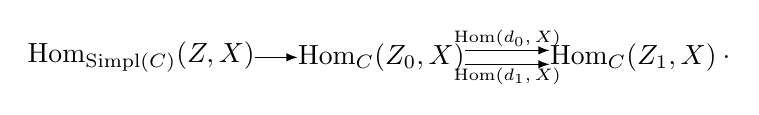
\begin{tikzpicture}[baseline=(b.base),>=latex]
    \node[inner sep=0pt] (a) at (0,0)
      {$\operatorname{Hom}_{\operatorname{Simpl}(C)}(Z,X)$};
    \node[inner sep=0pt] (b) at (3.05,0)
      {$\operatorname{Hom}_{C}(Z_0,X)$};
    \node[inner sep=0pt] (c) at (6.25,0)
      {$\operatorname{Hom}_{C}(Z_1,X)$};
    \draw[->] (a) -- (b);
    \draw[->]
      ([yshift=2.5bp]b.east) --
      node[above,inner sep=1bp,font=\fontsize{5.7}{6.4}\selectfont]
        {$\operatorname{Hom}(d_0,X)$}
      ([yshift=2.5bp]c.west);
    \draw[->]
      ([yshift=-2.5bp]b.east) --
      node[below,inner sep=1bp,font=\fontsize{5.7}{6.4}\selectfont]
        {$\operatorname{Hom}(d_1,X)$}
      ([yshift=-2.5bp]c.west);
    \node[anchor=west,inner sep=0pt,outer sep=0pt] at ([xshift=2bp]c.east) {.};
  \end{tikzpicture}%
}

% END SOURCE tex/common/eq1.tex


% BEGIN SOURCE tex/common/hom1.tex
% Native-TeX homotopy diagrams from LNM 239, physical p.21 / printed p.3.
\newcommand{\IllusieHomotopyTriangle}{%
  \begin{center}
  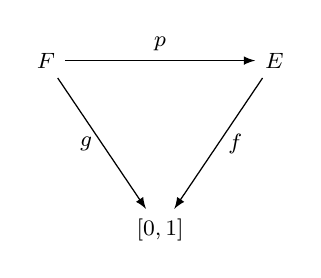
\begin{tikzpicture}[
    >=latex,
    line width=0.45pt,
    every node/.style={font=\rmfamily\fontsize{8}{9}\selectfont}
  ]
    \node (F) at (-1.45,1.0) {$F$};
    \node (E) at (1.45,1.0) {$E$};
    \node (I) at (0,-1.15) {$[0,1]$};
    \draw[->] (F) -- node[above] {$p$} (E);
    \draw[->] (F) -- node[left] {$g$} (I);
    \draw[->] (E) -- node[right] {$f$} (I);
  \end{tikzpicture}
  \end{center}%
}

\newcommand{\IllusieHomotopySquare}{%
  \begin{center}
  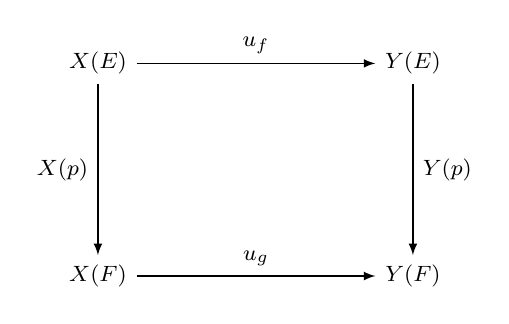
\begin{tikzpicture}[
    >=latex,
    line width=0.45pt,
    every node/.style={font=\rmfamily\fontsize{8}{9}\selectfont}
  ]
    \node (XE) at (-2.0,1.35) {$X(E)$};
    \node (YE) at (2.0,1.35) {$Y(E)$};
    \node (XF) at (-2.0,-1.35) {$X(F)$};
    \node (YF) at (2.0,-1.35) {$Y(F)$};
    \draw[->] (XE) -- node[above] {$u_f$} (YE);
    \draw[->] (XE) -- node[left] {$X(p)$} (XF);
    \draw[->] (YE) -- node[right] {$Y(p)$} (YF);
    \draw[->] (XF) -- node[above] {$u_g$} (YF);
  \end{tikzpicture}
  \end{center}%
}

% END SOURCE tex/common/hom1.tex


% BEGIN SOURCE tex/common/hom2.tex
% Native-TeX pullback square from LNM 239, physical p.58 / printed p.40.
\newcommand{\IllusieHomsPullbackSquare}{%
  \begin{center}
  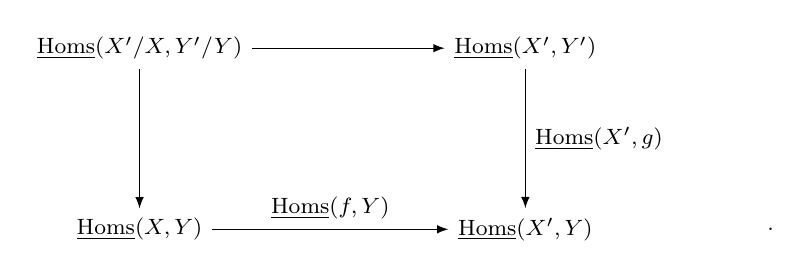
\begin{tikzpicture}[
    >=latex,
    line width=0.42pt,
    every node/.style={font=\rmfamily\fontsize{8.15}{8.8}\selectfont}
  ]
    \node (TL) at (-2.45, 1.15)
      {$\underline{\operatorname{Homs}}(X'/X,Y'/Y)$};
    \node (TR) at ( 2.45, 1.15)
      {$\underline{\operatorname{Homs}}(X',Y')$};
    \node (BL) at (-2.45,-1.15)
      {$\underline{\operatorname{Homs}}(X,Y)$};
    \node (BR) at ( 2.45,-1.15)
      {$\underline{\operatorname{Homs}}(X',Y)$};
    \draw[->] (TL) -- (TR);
    \draw[->] (TL) -- (BL);
    \draw[->] (TR) -- node[right]
      {$\underline{\operatorname{Homs}}(X',g)$} (BR);
    \draw[->] (BL) -- node[above]
      {$\underline{\operatorname{Homs}}(f,Y)$} (BR);
    \node[anchor=west] at (5.4,-1.15) {.};
  \end{tikzpicture}
  \end{center}%
}

% END SOURCE tex/common/hom2.tex


% BEGIN SOURCE tex/common/hom3.tex
% Native-TeX mapping-cylinder diagrams from LNM 239, physical p.62 / printed p.44.
\newcommand{\IllusieMappingCylinderTriangle}{%
  \begin{center}
  \begin{tikzpicture}[
    >=latex,
    line width=0.44pt,
    every node/.style={font=\rmfamily\fontsize{8.4}{9}\selectfont}
  ]
    \node (Yp) at (0,1.18) {$Y'$};
    \node (X)  at (-1.65,-0.92) {$X$};
    \node (Y)  at ( 1.65,-0.92) {$Y$};
    \draw[right hook->] (X) -- node[left] {$i$} (Yp);
    \draw[->] (Yp) -- node[right] {$p$} (Y);
    \draw[->] (X) -- node[above] {$f$} (Y);
    \node at (2.35,-0.92) {,};
  \end{tikzpicture}
  \end{center}%
}

\newcommand{\IllusieMappingCylinderPushout}{%
  \begin{center}
  \begin{tikzpicture}[
    >=latex,
    line width=0.44pt,
    every node/.style={font=\rmfamily\fontsize{8.4}{9}\selectfont}
  ]
    \node (DX) at (-2.00, 1.08) {$\Delta(1)\times X$};
    \node (Yp) at ( 2.00, 1.08) {$Y'$};
    \node (X)  at (-2.00,-1.08) {$X$};
    \node (Y)  at ( 2.00,-1.08) {$Y$};
    \draw[->] (DX) -- node[above] {$f'$} (Yp);
    \draw[right hook->] (X) -- node[left] {$d^1$} (DX);
    \draw[right hook->] (Y) -- node[right] {$j$} (Yp);
    \draw[->] (X) -- node[above] {$f$} (Y);
    \node at (2.70,-1.08) {,};
  \end{tikzpicture}
  \end{center}%
}

% END SOURCE tex/common/hom3.tex


% BEGIN SOURCE tex/common/hom4.tex
% Native fraction-calculus diagrams from LNM 239, physical p.63 / printed p.45.
\newcommand{\IllusieFractionProofSource}{%
  \begin{center}
  \begin{tikzpicture}[
    >=latex,line width=0.44pt,
    every node/.style={font=\rmfamily\fontsize{8.4}{9}\selectfont,inner sep=1pt}
  ]
    \node (Xp) at (0,1.15) {$X'$};
    \node (X)  at (0,0) {$X$};
    \node (Y)  at (2.25,0) {$Y$};
    \draw[->] (X) -- node[left] {$s$} (Xp);
    \draw[->] (X) -- node[above] {$u$} (Y);
    \node at (2.85,0) {,};
  \end{tikzpicture}
  \end{center}%
}

\newcommand{\IllusieFractionProofPushout}{%
  \begin{center}
  \begin{tikzpicture}[
    >=latex,line width=0.44pt,
    every node/.style={font=\rmfamily\fontsize{8.4}{9}\selectfont,inner sep=1pt}
  ]
    \node (Xp) at (-1.75,1.12) {$X'$};
    \node (Yp) at ( 1.75,1.12) {$Y'$};
    \node (X)  at (-1.75,0) {$X$};
    \node (Y)  at ( 1.75,0) {$Y$};
    \draw[->] (Xp) -- (Yp);
    \draw[right hook->] (X) -- node[left] {$s$} (Xp);
    \draw[right hook->] (Y) -- node[right] {$t$} (Yp);
    \draw[->] (X) -- (Y);
    \node at (4.15,0) {.};
  \end{tikzpicture}
  \end{center}%
}

\newcommand{\IllusieFractionProofParallel}{%
  \begin{center}
  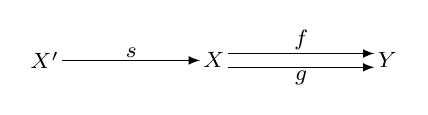
\begin{tikzpicture}[
    >=latex,line width=0.44pt,
    every node/.style={font=\rmfamily\fontsize{8.4}{9}\selectfont,inner sep=1pt}
  ]
    \node (Xp) at (-2.15,0) {$X'$};
    \node (X)  at (0,0) {$X$};
    \node (Y)  at (2.20,0) {$Y$};
    \draw[->] (Xp) -- node[above] {$s$} (X);
    \draw[->] ([yshift=2.5pt]X.east) -- node[above] {$f$} ([yshift=2.5pt]Y.west);
    \draw[->] ([yshift=-2.5pt]X.east) -- node[below] {$g$} ([yshift=-2.5pt]Y.west);
  \end{tikzpicture}
  \end{center}%
}

% END SOURCE tex/common/hom4.tex


% BEGIN SOURCE tex/common/hom5.tex
% Native pushout diagram from LNM 239, physical p.64 / printed p.46.
\newcommand{\IllusieCompositeHomotopyPushouts}{%
  \begin{center}
  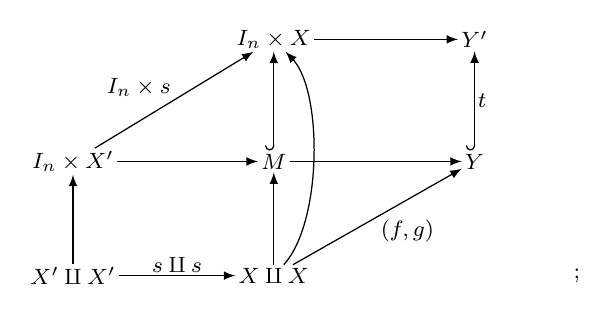
\begin{tikzpicture}[
    >=latex,x=1cm,y=1cm,line width=0.45pt,
    every node/.style={font=\rmfamily\fontsize{8}{9}\selectfont,inner sep=1pt}
  ]
    \node (IX)  at (0,1.55) {$I_n\times X$};
    \node (Yp)  at (2.55,1.55) {$Y'$};
    \node (IXp) at (-2.55,0) {$I_n\times X'$};
    \node (M)   at (0,0) {$M$};
    \node (Y)   at (2.55,0) {$Y$};
    \node (XXp) at (-2.55,-1.45) {$X'\amalg X'$};
    \node (XX)  at (0,-1.45) {$X\amalg X$};

    \draw[->] (IX) -- (Yp);
    \draw[right hook->] (Y) -- node[right] {$t$} (Yp);
    \draw[->] (IXp) -- (M);
    \draw[->] (M) -- (Y);
    \draw[->] (XXp) -- (IXp);
    \draw[->] (XXp) -- node[above] {$s\amalg s$} (XX);
    \draw[->] (XX) -- (M);
    \draw[->] (IXp) -- node[above left] {$I_n\times s$} (IX);
    \draw[right hook->] (M) -- (IX);
    \draw[->] (XX) .. controls (0.62,-0.77) and (0.62,0.90) .. (IX);
    \draw[->] (XX) -- node[below right] {$(f,g)$} (Y);
    \node at (3.85,-1.45) {$;$};
  \end{tikzpicture}
  \end{center}%
}

% END SOURCE tex/common/hom5.tex


% BEGIN SOURCE tex/common/hom6.tex
% Native lifting diagrams from LNM 239, physical p.65 / printed p.47.
\newcommand{\IllusieLocalLiftingSquare}{%
  \begin{center}
  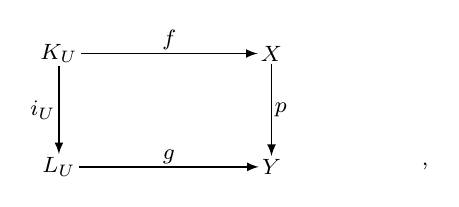
\begin{tikzpicture}[
    >=latex,x=1cm,y=1cm,line width=0.45pt,
    every node/.style={font=\rmfamily\fontsize{8}{9}\selectfont,inner sep=1pt}
  ]
    \node (KU) at (-1.35,0.72) {$K_U$};
    \node (X)  at (1.35,0.72) {$X$};
    \node (LU) at (-1.35,-0.72) {$L_U$};
    \node (Y)  at (1.35,-0.72) {$Y$};
    \draw[->] (KU) -- node[above] {$f$} (X);
    \draw[->] (KU) -- node[left] {$i_U$} (LU);
    \draw[->] (X) -- node[right] {$p$} (Y);
    \draw[->] (LU) -- node[above] {$g$} (Y);
  \node at (3.3,-.72) {,};
\end{tikzpicture}
  \end{center}%
}

\newcommand{\IllusieLocalLiftDiagram}{%
  \begin{center}
  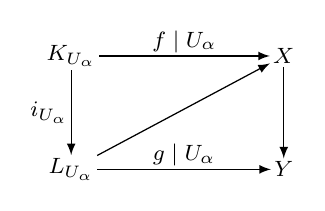
\begin{tikzpicture}[
    >=latex,x=1cm,y=1cm,line width=0.45pt,
    every node/.style={font=\rmfamily\fontsize{8}{9}\selectfont,inner sep=1pt}
  ]
    \node (KU) at (-1.35,0.72) {$K_{U_\alpha}$};
    \node (X)  at (1.35,0.72) {$X$};
    \node (LU) at (-1.35,-0.72) {$L_{U_\alpha}$};
    \node (Y)  at (1.35,-0.72) {$Y$};
    \draw[->] (KU) -- node[above] {$f\mid U_\alpha$} (X);
    \draw[->] (KU) -- node[left] {$i_{U_\alpha}$} (LU);
    \draw[->] (X) -- (Y);
    \draw[->] (LU) -- node[above] {$g\mid U_\alpha$} (Y);
    \draw[->] (LU) -- (X);
  \end{tikzpicture}
  \end{center}%
}

% END SOURCE tex/common/hom6.tex


% BEGIN SOURCE tex/common/tri1.tex
% Native-TeX transitivity triangle from LNM 239, physical p.12 / Roman X.
\newcommand{\IllusieTransitivityTriangle}{%
  \begin{center}
  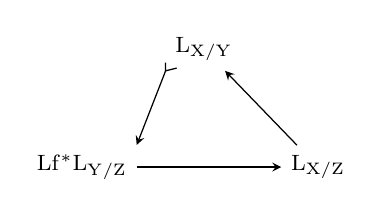
\begin{tikzpicture}[
    >=stealth,
    line width=0.45pt,
    every node/.style={font=\rmfamily\fontsize{8.15}{9}\selectfont}
  ]
    \node (xy) at (0,1.05) {$\mathrm{L}_{\mathrm{X}/\mathrm{Y}}$};
    \node (fyz) at (-1.55,-0.45) {$\mathrm{L}\mathrm{f}^{*}\mathrm{L}_{\mathrm{Y}/\mathrm{Z}}$};
    \node (xz) at (1.45,-0.45) {$\mathrm{L}_{\mathrm{X}/\mathrm{Z}}$};
    \draw[->] (xy.south west) -- (fyz.north east);
    % Printed two-stroke tail mark on the connecting edge.
    \draw ([yshift=3pt]xy.south west) -- (xy.south west)
      -- ([xshift=4pt,yshift=1pt]xy.south west);
    \draw[->] (fyz) -- (xz);
    \draw[->] (xz) -- (xy);
  \end{tikzpicture}
  \end{center}%
}

% END SOURCE tex/common/tri1.tex


% BEGIN SOURCE tex/common/guide1.tex
% Native chapter-dependency guide from LNM 239 physical p.17 / Roman XV.
\newcommand{\IllusieChapterGuide}{%
  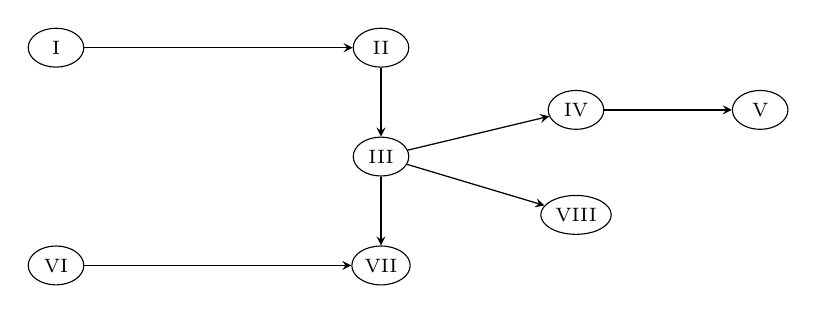
\begin{tikzpicture}[
    x=39bp,y=28bp,>=stealth,
    guide node/.style={draw,ellipse,minimum width=20bp,minimum height=14bp,
      inner sep=1.5bp,font=\fontsize{7}{7}\selectfont},
    guide arrow/.style={->,line width=0.45pt}
  ]
    \node[guide node] (I) at (0,2.8) {I};
    \node[guide node] (II) at (3,2.8) {II};
    \node[guide node] (III) at (3,1.4) {III};
    \node[guide node] (IV) at (4.8,2.0) {IV};
    \node[guide node] (V) at (6.5,2.0) {V};
    \node[guide node] (VIII) at (4.8,0.65) {VIII};
    \node[guide node] (VII) at (3,0) {VII};
    \node[guide node] (VI) at (0,0) {VI};
    \draw[guide arrow] (I) -- (II);
    \draw[guide arrow] (II) -- (III);
    \draw[guide arrow] (III) -- (IV);
    \draw[guide arrow] (IV) -- (V);
    \draw[guide arrow] (III) -- (VIII);
    \draw[guide arrow] (III) -- (VII);
    \draw[guide arrow] (VI) -- (VII);
  \end{tikzpicture}%
}

% END SOURCE tex/common/guide1.tex


% BEGIN SOURCE tex/common/assoc1.tex
% Native-TeX associativity/coassociativity squares from LNM 239,
% physical p.26 / printed p.8, formula (1.2.2.3).
\newcommand{\IllusieAssociativitySquares}{%
  \begin{center}
  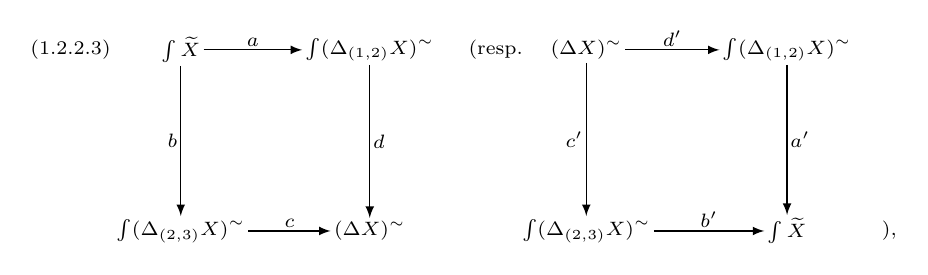
\begin{tikzpicture}[
    >=latex,
    x=1cm,
    y=1cm,
    line width=0.45pt,
    every node/.style={font=\rmfamily\fontsize{7.2}{8}\selectfont,inner sep=1pt}
  ]
    \node at (-6.35,1.15) {(1.2.2.3)};

    \node (LTL) at (-4.95,1.15) {$\int\widetilde X$};
    \node (LTR) at (-2.55,1.15) {$\int(\Delta_{(1,2)}X)^{\sim}$};
    \node (LBL) at (-4.95,-1.15) {$\int(\Delta_{(2,3)}X)^{\sim}$};
    \node (LBR) at (-2.55,-1.15) {$(\Delta X)^{\sim}$};
    \draw[->] (LTL) -- node[above] {$a$} (LTR);
    \draw[->] (LTL) -- node[left] {$b$} (LBL);
    \draw[->] (LBL) -- node[above] {$c$} (LBR);
    \draw[->] (LTR) -- node[right] {$d$} (LBR);

    \node at (-0.95,1.15) {(resp.};
    \node (RTL) at (0.20,1.15) {$(\Delta X)^{\sim}$};
    \node (RTR) at (2.75,1.15) {$\int(\Delta_{(1,2)}X)^{\sim}$};
    \node (RBL) at (0.20,-1.15) {$\int(\Delta_{(2,3)}X)^{\sim}$};
    \node (RBR) at (2.75,-1.15) {$\int\widetilde X$};
    \draw[->] (RTL) -- node[above] {$d'$} (RTR);
    \draw[->] (RTL) -- node[left] {$c'$} (RBL);
    \draw[->] (RBL) -- node[above] {$b'$} (RBR);
    \draw[->] (RTR) -- node[right] {$a'$} (RBR);
    \node at (4.05,-1.15) {),};
  \end{tikzpicture}
  \end{center}%
}

% END SOURCE tex/common/assoc1.tex


% BEGIN SOURCE tex/common/dold1.tex
% Native-TeX factorization square from LNM 239,
% physical p.27 / printed p.9, section 1.3.1.
\newcommand{\IllusieDoldPuppeSquare}{%
  \begin{center}
  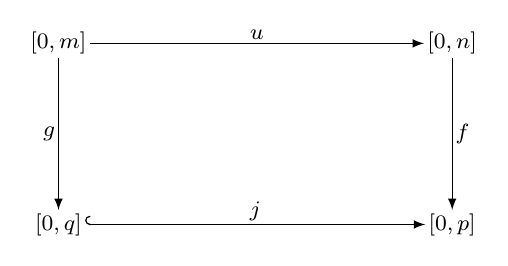
\begin{tikzpicture}[
    >=latex,
    x=1cm,
    y=1cm,
    line width=0.45pt,
    every node/.style={font=\rmfamily\fontsize{8}{9}\selectfont,inner sep=1pt}
  ]
    \node (TL) at (-2.5,1.15) {$[0,m]$};
    \node (TR) at (2.5,1.15) {$[0,n]$};
    \node (BL) at (-2.5,-1.15) {$[0,q]$};
    \node (BR) at (2.5,-1.15) {$[0,p]$};
    \draw[->] (TL) -- node[above] {$u$} (TR);
    \draw[->] (TL) -- node[left] {$g$} (BL);
    \draw[->] (TR) -- node[right] {$f$} (BR);
    \draw[right hook->] (BL) -- node[above] {$j$} (BR);
  \end{tikzpicture}
  \end{center}%
}

% END SOURCE tex/common/dold1.tex


% BEGIN SOURCE tex/common/dold2.tex
% Native normal/degenerate restriction diagram from LNM 239,
% physical p.29 / printed p.11, section 1.3.5.
\newcommand{\IllusieNormalDegenerateDiagram}{%
  \begin{center}
  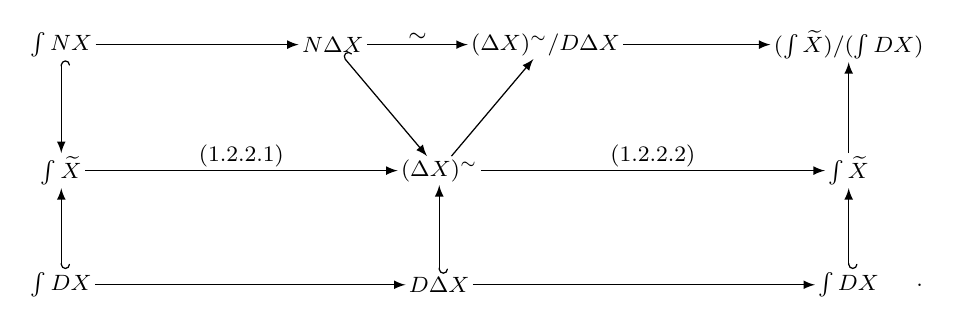
\begin{tikzpicture}[
    >=latex,
    x=1cm,
    y=1cm,
    line width=0.45pt,
    every node/.style={font=\rmfamily\fontsize{8}{9}\selectfont,inner sep=1pt}
  ]
    \node (TL) at (-4.8,1.6) {$\int NX$};
    \node (TC) at (-1.35,1.6) {$N\Delta X$};
    \node (TQ) at (1.35,1.6) {$(\Delta X)^{\sim}/D\Delta X$};
    \node (TR) at (5.2,1.6) {$(\int\widetilde X)/(\int DX)$};
    \node (ML) at (-4.8,0) {$\int\widetilde X$};
    \node (MC) at (0,0) {$(\Delta X)^{\sim}$};
    \node (MR) at (5.2,0) {$\int\widetilde X$};
    \node (BL) at (-4.8,-1.45) {$\int DX$};
    \node (BC) at (0,-1.45) {$D\Delta X$};
    \node (BR) at (5.2,-1.45) {$\int DX$};
    \draw[->] (TL) -- (TC);
    \draw[->] (TC) -- node[above] {$\sim$} (TQ);
    \draw[->] (TQ) -- (TR);
    \draw[->] (ML) -- node[above] {(1.2.2.1)} (MC);
    \draw[->] (MC) -- node[above] {(1.2.2.2)} (MR);
    \draw[->] (BL) -- (BC);
    \draw[->] (BC) -- (BR);
    \draw[right hook->] (TL) -- (ML);
    \draw[right hook->] (TC) -- (MC);
    \draw[->] (MC) -- (TQ);
    \draw[->] (MR) -- (TR);
    \draw[left hook->] (BL) -- (ML);
    \draw[left hook->] (BC) -- (MC);
    \draw[left hook->] (BR) -- (MR);
    \node at (6.1,-1.45) {.};
  \end{tikzpicture}
  \end{center}%
}

% END SOURCE tex/common/dold2.tex


% BEGIN SOURCE tex/common/fractions1.tex
% Native right/left calculus-of-fractions diagrams from LNM 239,
% physical p.30 / printed p.12, section 1.4.2.
\newcommand{\IllusieRightFractionFrThreeSource}{%
  \begin{center}
  \begin{tikzpicture}[
    >=latex,x=1cm,y=1cm,line width=0.45pt,
    every node/.style={font=\rmfamily\fontsize{8}{9}\selectfont,inner sep=1pt}
  ]
    \node (X) at (-1.7,0) {$X$};
    \node (Y) at (1.7,0) {$Y$};
    \node (Yp) at (1.7,1.35) {$Y'$};
    \draw[->] (X) -- node[above] {$u$} (Y);
    \draw[->] (Yp) -- node[right] {$t$} (Y);
  \end{tikzpicture}
  \end{center}%
}

\newcommand{\IllusieRightFractionFrThreeCompletion}{%
  \begin{center}
  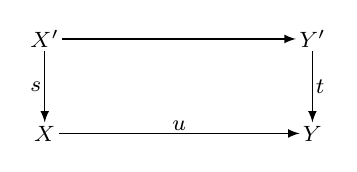
\begin{tikzpicture}[
    >=latex,x=1cm,y=1cm,line width=0.45pt,
    every node/.style={font=\rmfamily\fontsize{8}{9}\selectfont,inner sep=1pt}
  ]
    \node (Xp) at (-1.7,1.2) {$X'$};
    \node (Yp) at (1.7,1.2) {$Y'$};
    \node (X) at (-1.7,0) {$X$};
    \node (Y) at (1.7,0) {$Y$};
    \draw[->] (Xp) -- (Yp);
    \draw[->] (Xp) -- node[left] {$s$} (X);
    \draw[->] (Yp) -- node[right] {$t$} (Y);
    \draw[->] (X) -- node[above] {$u$} (Y);
  \end{tikzpicture}
  \end{center}%
}

\newcommand{\IllusieRightFractionFrFourSource}{%
  \begin{center}
  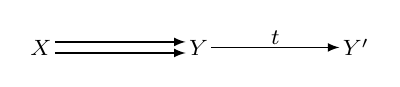
\begin{tikzpicture}[
    >=latex,x=1cm,y=1cm,line width=0.45pt,
    every node/.style={font=\rmfamily\fontsize{8}{9}\selectfont,inner sep=1pt}
  ]
    \node (X) at (-2.0,0) {$X$};
    \node (Y) at (0,0) {$Y$};
    \node (Yp) at (2.0,0) {$Y'$};
    \draw[->] ([yshift=2pt]X.east) -- ([yshift=2pt]Y.west);
    \draw[->] ([yshift=-2pt]X.east) -- ([yshift=-2pt]Y.west);
    \draw[->] (Y) -- node[above] {$t$} (Yp);
  \end{tikzpicture}
  \end{center}%
}

\newcommand{\IllusieRightFractionFrFourCompletion}{%
  \begin{center}
  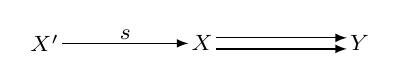
\begin{tikzpicture}[
    >=latex,x=1cm,y=1cm,line width=0.45pt,
    every node/.style={font=\rmfamily\fontsize{8}{9}\selectfont,inner sep=1pt}
  ]
    \node (Xp) at (-2.0,0) {$X'$};
    \node (X) at (0,0) {$X$};
    \node (Y) at (2.0,0) {$Y$};
    \draw[->] (Xp) -- node[above] {$s$} (X);
    \draw[->] ([yshift=2pt]X.east) -- ([yshift=2pt]Y.west);
    \draw[->] ([yshift=-2pt]X.east) -- ([yshift=-2pt]Y.west);
  \end{tikzpicture}
  \end{center}%
}

\newcommand{\IllusieLeftFractionFrThreeSource}{%
  \begin{center}
  \begin{tikzpicture}[
    >=latex,x=1cm,y=1cm,line width=0.45pt,
    every node/.style={font=\rmfamily\fontsize{8}{9}\selectfont,inner sep=1pt}
  ]
    \node (X) at (-1.5,0.8) {$X$};
    \node (Y) at (1.5,0.8) {$Y$};
    \node (Xp) at (-1.5,-0.65) {$X'$};
    \draw[->] (X) -- node[above] {$u$} (Y);
    \draw[->] (X) -- node[left] {$s$} (Xp);
  \end{tikzpicture}
  \end{center}%
}

\newcommand{\IllusieLeftFractionFrThreeCompletion}{%
  \begin{center}
  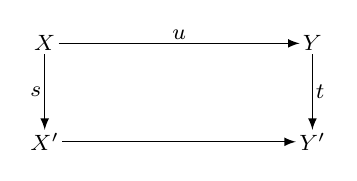
\begin{tikzpicture}[
    >=latex,x=1cm,y=1cm,line width=0.45pt,
    every node/.style={font=\rmfamily\fontsize{8}{9}\selectfont,inner sep=1pt}
  ]
    \node (X) at (-1.7,1.25) {$X$};
    \node (Y) at (1.7,1.25) {$Y$};
    \node (Xp) at (-1.7,0) {$X'$};
    \node (Yp) at (1.7,0) {$Y'$};
    \draw[->] (X) -- node[above] {$u$} (Y);
    \draw[->] (X) -- node[left] {$s$} (Xp);
    \draw[->] (Y) -- node[right] {$t$} (Yp);
    \draw[->] (Xp) -- (Yp);
  \end{tikzpicture}
  \end{center}%
}

\newcommand{\IllusieLeftFractionFrFourSource}{%
  \begin{center}
  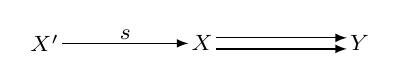
\begin{tikzpicture}[
    >=latex,x=1cm,y=1cm,line width=0.45pt,
    every node/.style={font=\rmfamily\fontsize{8}{9}\selectfont,inner sep=1pt}
  ]
    \node (Xp) at (-2.0,0) {$X'$};
    \node (X) at (0,0) {$X$};
    \node (Y) at (2.0,0) {$Y$};
    \draw[->] (Xp) -- node[above] {$s$} (X);
    \draw[->] ([yshift=2pt]X.east) -- ([yshift=2pt]Y.west);
    \draw[->] ([yshift=-2pt]X.east) -- ([yshift=-2pt]Y.west);
  \end{tikzpicture}
  \end{center}%
}

\newcommand{\IllusieLeftFractionFrFourCompletion}{%
  \begin{center}
  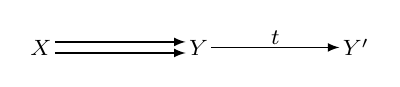
\begin{tikzpicture}[
    >=latex,x=1cm,y=1cm,line width=0.45pt,
    every node/.style={font=\rmfamily\fontsize{8}{9}\selectfont,inner sep=1pt}
  ]
    \node (X) at (-2.0,0) {$X$};
    \node (Y) at (0,0) {$Y$};
    \node (Yp) at (2.0,0) {$Y'$};
    \draw[->] ([yshift=2pt]X.east) -- ([yshift=2pt]Y.west);
    \draw[->] ([yshift=-2pt]X.east) -- ([yshift=-2pt]Y.west);
    \draw[->] (Y) -- node[above] {$t$} (Yp);
  \end{tikzpicture}
  \end{center}%
}

% END SOURCE tex/common/fractions1.tex


% BEGIN SOURCE tex/common/derived1.tex
% Native 2-cell diagram from LNM 239, physical p.32 / printed p.14,
% section 1.4.4. The 2-cell v has target F, as does u_F.
\newcommand{\IllusieLeftDerivedUniversalTriangle}{%
  \begin{center}
  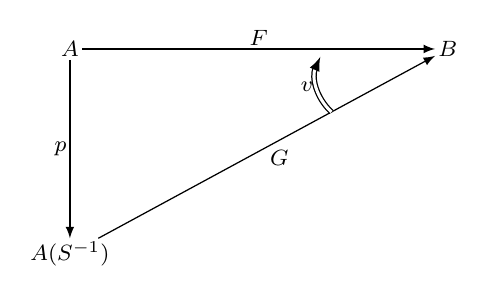
\begin{tikzpicture}[
    >=latex,x=1cm,y=1cm,line width=0.45pt,
    every node/.style={font=\rmfamily\fontsize{8}{9}\selectfont,inner sep=1pt}
  ]
    \node (A) at (-2.4,1.5) {$A$};
    \node (AS) at (-2.4,-1.1) {$A(S^{-1})$};
    \node (B) at (2.4,1.5) {$B$};
    \draw[->] (A) -- node[above] {$F$} (B);
    \draw[->] (A) -- node[left] {$p$} (AS);
    \draw[->] (AS) -- node[below right] {$G$} (B);
    \draw[double distance=1.1pt,->]
      (0.92,0.70) to[bend left=35] node[left] {$v$} (0.78,1.40);
  \end{tikzpicture}
  \end{center}%
}

% END SOURCE tex/common/derived1.tex


% BEGIN SOURCE tex/common/derived2.tex
% Native comparison grid from LNM 239, physical p.33 / printed p.15,
% section 1.4.5. Horizontal arrows are N and K; vertical arrows localize.
\newcommand{\IllusieDerivedComparisonGrid}{%
  \begin{center}
  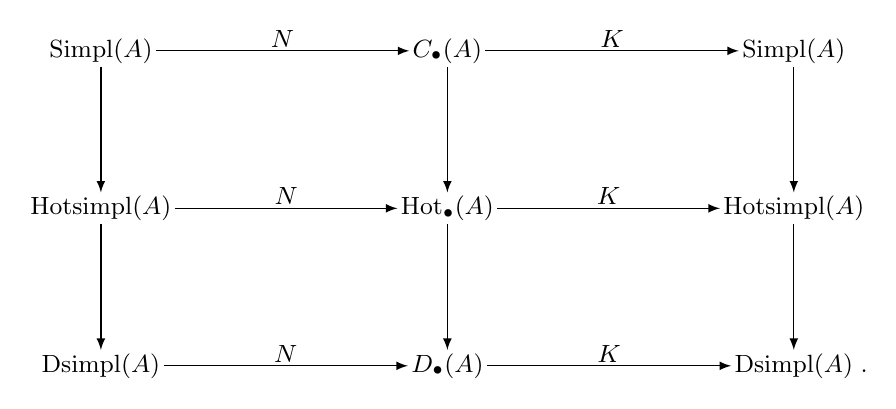
\begin{tikzpicture}[
    >=latex,x=1cm,y=1cm,line width=0.45pt,
    every node/.style={font=\rmfamily\fontsize{9}{10}\selectfont,inner sep=1pt}
  ]
    \node (s0) at (-4.4,2) {$\operatorname{Simpl}(A)$};
    \node (c0) at (0,2) {$C_{\bullet}(A)$};
    \node (s1) at (4.4,2) {$\operatorname{Simpl}(A)$};
    \node (hs0) at (-4.4,0) {$\operatorname{Hotsimpl}(A)$};
    \node (hc0) at (0,0) {$\operatorname{Hot}_{\bullet}(A)$};
    \node (hs1) at (4.4,0) {$\operatorname{Hotsimpl}(A)$};
    \node (ds0) at (-4.4,-2) {$\operatorname{Dsimpl}(A)$};
    \node (dc0) at (0,-2) {$D_{\bullet}(A)$};
    \node (ds1) at (4.4,-2) {$\operatorname{Dsimpl}(A)$};

    \draw[->] (s0) -- node[above] {$N$} (c0);
    \draw[->] (c0) -- node[above] {$K$} (s1);
    \draw[->] (hs0) -- node[above] {$N$} (hc0);
    \draw[->] (hc0) -- node[above] {$K$} (hs1);
    \draw[->] (ds0) -- node[above] {$N$} (dc0);
    \draw[->] (dc0) -- node[above] {$K$} (ds1);

    \draw[->] (s0) -- (hs0);
    \draw[->] (c0) -- (hc0);
    \draw[->] (s1) -- (hs1);
    \draw[->] (hs0) -- (ds0);
    \draw[->] (hc0) -- (dc0);
    \draw[->] (hs1) -- (ds1);
    \node[anchor=base west,inner sep=0pt,outer sep=0pt] at ([xshift=1.5pt]ds1.base east) {.};
  \end{tikzpicture}
  \end{center}%
}

% END SOURCE tex/common/derived2.tex


% BEGIN SOURCE tex/common/local2.tex
% Native-TeX diagrams for Lemma 2.2.6, LNM 239 physical p.47 / printed p.29.
\newcommand{\IllusieLocalObjectSquare}{%
  \begin{center}
  \begin{tikzpicture}[
    >=latex,
    line width=0.45pt,
    every node/.style={font=\rmfamily\fontsize{9.3}{10.4}\selectfont}
  ]
    \node (Ei) at (-2.0,1.55) {$E_i$};
    \node (Fi) at ( 2.0,1.55) {$F_i$};
    \node (EU) at (-2.0,-1.55) {$E(U)$};
    \node (FU) at ( 2.0,-1.55) {$F(U)$};
    \draw[->] (Ei) -- node[above] {$u_i$} (Fi);
    \draw[->] (Ei) -- (EU);
    \draw[->] (Fi) -- (FU);
    \draw[->] (EU) -- node[above] {$u(U)$} (FU);
    \node at (2.55,-1.55) {,};
  \end{tikzpicture}
  \end{center}%
}

\newcommand{\IllusieLocalRestrictionSquare}{%
  \begin{center}
  \begin{tikzpicture}[
    >=latex,
    line width=0.45pt,
    every node/.style={font=\rmfamily\fontsize{9.3}{10.4}\selectfont}
  ]
    \node (Ei) at (-2.0,1.55) {$E_i$};
    \node (Fi) at ( 2.0,1.55) {$F_i$};
    \node (EU) at (-2.0,-1.55) {$E\vert U$};
    \node (FU) at ( 2.0,-1.55) {$F\vert U$};
    \draw[->] (Ei) -- node[above] {$u_i$} (Fi);
    \draw[->] (Ei) -- (EU);
    \draw[->] (Fi) -- (FU);
    \draw[->] (EU) -- node[above] {$u\vert U$} (FU);
    \node at (2.55,-1.55) {,};
  \end{tikzpicture}
  \end{center}%
}

\newcommand{\IllusieLocalMorphismTriangle}{%
  \begin{center}
  \begin{tikzpicture}[
    >=latex,
    line width=0.45pt,
    every node/.style={font=\rmfamily\fontsize{9.3}{10.4}\selectfont}
  ]
    \node (ui) at (-1.75,1.25) {$u_i$};
    \node (uj) at ( 1.75,1.25) {$u_j$};
    \node (u)  at (0,-1.25) {$u(U)$};
    \draw[->] (ui) -- node[above] {$f$} (uj);
    \draw[->] (ui) -- node[left] {$i$} (u);
    \draw[->] (uj) -- node[right] {$j$} (u);
    \node at (2.25,-1.25) {.};
  \end{tikzpicture}
  \end{center}%
}

% END SOURCE tex/common/local2.tex


% BEGIN SOURCE tex/common/local3.tex
% Native-TeX diagram for Lemma 2.2.6, LNM 239 physical p.48 / printed p.30.
\newcommand{\IllusieFinitePresentationCube}{%
  \begin{center}
  \begin{tikzpicture}[
    x=1.15cm,
    y=1.40cm,
    >=latex,
    line width=0.45pt,
    every node/.style={font=\rmfamily\fontsize{8.8}{9.8}\selectfont}
  ]
    \node (A0) at (-3.2, 2.6) {$A$};
    \node (A1) at ( 1.2, 2.6) {$A$};
    \node (B0) at (-1.3, 1.1) {$A$};
    \node (B1) at ( 3.1, 1.1) {$A$};
    \node (E0) at (-3.2,-0.8) {$E^n(U)$};
    \node (E1) at ( 1.2,-0.8) {$E^{n+1}(U)$};
    \node (F0) at (-1.3,-2.3) {$F^n(U)$};
    \node (F1) at ( 3.1,-2.3) {$F^{n+1}(U)$};
    \draw[->] (A0) -- node[above] {$\operatorname{Id}$} (A1);
    \draw[->] (A0) -- node[above left] {$\operatorname{Id}$} (B0);
    \draw[->] (A1) -- node[above right] {$\operatorname{Id}$} (B1);
    \draw[->] (B0) -- node[above] {$\operatorname{Id}$} (B1);
    \draw[->] (A0) -- node[left] {$x$} (E0);
    \draw[->] (A1) -- node[right] {$dx$} (E1);
    \draw[->] (B0) -- node[left] {$u(U)x$} (F0);
    \draw[->] (B1) -- node[right] {$d\,u(U)x(=u(U)dx)$} (F1);
    \draw[->] (E0) -- node[above] {$d$} (E1);
    \draw[->] (F0) -- node[above] {$d$} (F1);
    \draw[->] (E0) -- node[below left] {$u(U)$} (F0);
    \draw[->] (E1) -- node[below left] {$u(U)$} (F1);
  \end{tikzpicture}
  \end{center}%
}

% END SOURCE tex/common/local3.tex


% BEGIN SOURCE tex/common/local4.tex
% Native-TeX diagram for Lemma 2.2.7, LNM 239 physical p.49 / printed p.31.
\newcommand{\IllusieExtensionLemmaTriangle}{%
  \begin{center}
  \begin{tikzpicture}[
    >=latex,
    line width=0.42pt,
    every node/.style={font=\rmfamily\fontsize{8.15}{9.2}\selectfont}
  ]
    \node (z0) at (-4.10, 1.15) {$0$};
    \node (up) at (-2.55, 1.15) {$u'$};
    \node (upp) at (-0.35, 1.15) {$u''_{\alpha}$};
    \node (va) at ( 1.95, 1.15) {$v_{\alpha}$};
    \node (z1) at ( 3.75, 1.15) {$0$};
    \node (ua) at (-1.20,-1.55) {$u(U_{\alpha})$};
    \draw[->] (z0) -- (up);
    \draw[->] (up) -- (upp);
    \draw[->] (upp) -- (va);
    \draw[->] (va) -- (z1);
    \draw[->] (up) -- node[below left] {$f\vert U_{\alpha}$} (ua);
    \draw[->] (upp) -- (ua);
    \node at (2.95,-1.55) {,};
  \end{tikzpicture}
  \end{center}%
}

% END SOURCE tex/common/local4.tex


% BEGIN SOURCE tex/common/local5.tex
% Native-TeX diagrams for Lemma 2.2.7, LNM 239 physical p.50 / printed p.32.
\newcommand{\IllusieRTSquare}{%
  \begin{center}
  \begin{tikzpicture}[>=latex,line width=0.42pt,every node/.style={font=\rmfamily\fontsize{8.15}{9.2}\selectfont}]
    \node (M)  at (-2.80, 1.15) {$M$};
    \node (ZE) at ( 1.75, 1.15) {$Z^{n+1}(E')$};
    \node (Fn) at (-2.80,-1.15) {$F'^{n}$};
    \node (ZF) at ( 1.75,-1.15) {$Z^{n+1}(F')$};
    \draw[->] (M) -- node[above] {$r$} (ZE);
    \draw[->] (M) -- node[left] {$t$} (Fn);
    \draw[->] (ZE) -- node[right] {$u'$} (ZF);
    \draw[->] (Fn) -- (ZF);
    \node at (3.35,-1.15) {.};
  \end{tikzpicture}
  \end{center}%
}

\newcommand{\IllusieCohomologyRectangle}{%
  \begin{center}
  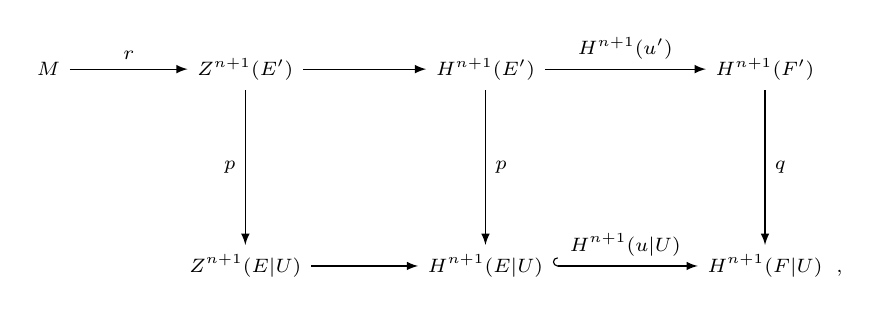
\begin{tikzpicture}[>=latex,line width=0.42pt,every node/.style={font=\rmfamily\fontsize{7.4}{8.5}\selectfont}]
    \node (M)   at (-5.65, 1.20) {$M$};
    \node (ZE)  at (-3.15, 1.20) {$Z^{n+1}(E')$};
    \node (HE)  at (-0.10, 1.20) {$H^{n+1}(E')$};
    \node (HF)  at ( 3.45, 1.20) {$H^{n+1}(F')$};
    \node (ZEU) at (-3.15,-1.30) {$Z^{n+1}(E\vert U)$};
    \node (HEU) at (-0.10,-1.30) {$H^{n+1}(E\vert U)$};
    \node (HFU) at ( 3.45,-1.30) {$H^{n+1}(F\vert U)$};
    \draw[->] (M) -- node[above] {$r$} (ZE);
    \draw[->] (ZE) -- (HE);
    \draw[->] (HE) -- node[above] {$H^{n+1}(u')$} (HF);
    \draw[->] (ZE) -- node[left] {$p$} (ZEU);
    \draw[->] (HE) -- node[right] {$p$} (HEU);
    \draw[->] (HF) -- node[right] {$q$} (HFU);
    \draw[->] (ZEU) -- (HEU);
    \draw[right hook->] (HEU) -- node[above] {$H^{n+1}(u\vert U)$} (HFU);
    \node[anchor=base west,inner sep=0pt,outer sep=0pt] at ([xshift=1.5pt]HFU.base east) {,};
  \end{tikzpicture}
  \end{center}%
}

\newcommand{\IllusieLocalizedSSquare}{%
  \begin{center}
  \begin{tikzpicture}[>=latex,line width=0.42pt,every node/.style={font=\rmfamily\fontsize{8.15}{9.2}\selectfont}]
    \node (M)   at (-2.80, 1.15) {$M$};
    \node (ZE)  at ( 1.75, 1.15) {$Z^{n+1}(E')$};
    \node (EnU) at (-2.80,-1.15) {$E^{n}\vert U$};
    \node (ZEU) at ( 1.75,-1.15) {$Z^{n+1}(E\vert U)$};
    \draw[->] (M) -- node[above] {$r$} (ZE);
    \draw[->] (M) -- node[left] {$s$} (EnU);
    \draw[->] (ZE) -- (ZEU);
    \draw[->] (EnU) -- (ZEU);
    \node[anchor=base west,inner sep=0pt,outer sep=0pt] at ([xshift=1.5pt]ZEU.base east) {.};
  \end{tikzpicture}
  \end{center}%
}

\newcommand{\IllusieTSQUquare}{%
  \begin{center}
  \begin{tikzpicture}[>=latex,line width=0.42pt,every node/.style={font=\rmfamily\fontsize{8.15}{9.2}\selectfont}]
    \node (M)   at (-2.80, 1.15) {$M$};
    \node (Fpn) at ( 1.75, 1.15) {$F'^{n}$};
    \node (EnU) at (-2.80,-1.15) {$E^{n}\vert U$};
    \node (FnU) at ( 1.75,-1.15) {$F^{n}\vert U$};
    \draw[->] (M) -- node[above] {$t$} (Fpn);
    \draw[->] (M) -- node[left] {$s$} (EnU);
    \draw[->] (Fpn) -- node[right] {$q$} (FnU);
    \draw[->] (EnU) -- node[above] {$u$} (FnU);
  \end{tikzpicture}
  \end{center}%
}

% END SOURCE tex/common/local5.tex


% BEGIN SOURCE tex/common/local6.tex
% Native-TeX diagrams for Lemma 2.2.7, LNM 239 physical p.51 / printed p.33.
\newcommand{\IllusieUDoublePrimeComplexMap}{%
  \begin{center}
  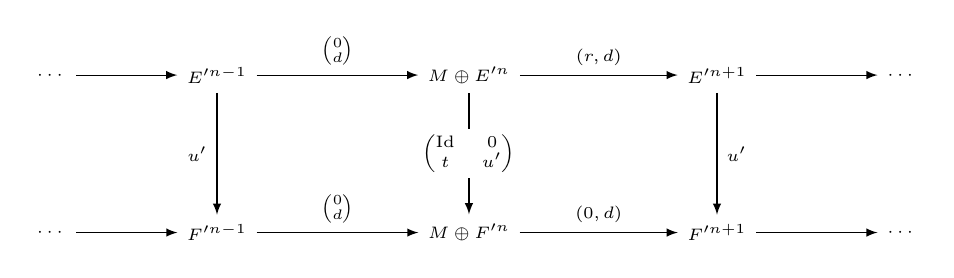
\begin{tikzpicture}[>=latex,line width=0.4pt,every node/.style={font=\rmfamily\fontsize{5.7}{6.2}\selectfont}]
    \node (ET0) at (-5.65, 1.00) {$\cdots$};
    \node (ET1) at (-3.55, 1.00) {$E'^{n-1}$};
    \node (ET2) at (-0.35, 1.00) {$M\oplus E'^n$};
    \node (ET3) at ( 2.80, 1.00) {$E'^{n+1}$};
    \node (ET4) at ( 5.15, 1.00) {$\cdots$};
    \node (FB0) at (-5.65,-1.00) {$\cdots$};
    \node (FB1) at (-3.55,-1.00) {$F'^{n-1}$};
    \node (FB2) at (-0.35,-1.00) {$M\oplus F'^n$};
    \node (FB3) at ( 2.80,-1.00) {$F'^{n+1}$};
    \node (FB4) at ( 5.15,-1.00) {$\cdots$};
    \draw[->] (ET0) -- (ET1); \draw[->] (ET1) -- node[above] {$\binom{0}{d}$} (ET2);
    \draw[->] (ET2) -- node[above] {$(r,d)$} (ET3); \draw[->] (ET3) -- (ET4);
    \draw[->] (FB0) -- (FB1); \draw[->] (FB1) -- node[above] {$\binom{0}{d}$} (FB2);
    \draw[->] (FB2) -- node[above] {$(0,d)$} (FB3); \draw[->] (FB3) -- (FB4);
    \draw[->] (ET1) -- node[left] {$u'$} (FB1);
    \draw[->] (ET2) -- node[fill=white,inner sep=2pt] {$\begin{pmatrix}\mathrm{Id}&0\\ t&u'\end{pmatrix}$} (FB2);
    \draw[->] (ET3) -- node[right] {$u'$} (FB3);
  \end{tikzpicture}
  \end{center}%
}

\newcommand{\IllusiePPrimeComplexMap}{%
  \begin{center}
  \begin{tikzpicture}[>=latex,line width=0.4pt,every node/.style={font=\rmfamily\fontsize{5.7}{6.2}\selectfont}]
    \node (ET0) at (-5.65, 1.00) {$\cdots$};
    \node (ET1) at (-3.55, 1.00) {$E'^{n-1}$};
    \node (ET2) at (-0.35, 1.00) {$M\oplus E'^n$};
    \node (ET3) at ( 2.80, 1.00) {$E'^{n+1}$};
    \node (ET4) at ( 5.15, 1.00) {$\cdots$};
    \node at (5.75,1.00) {,};
    \node (EB0) at (-5.65,-1.00) {$\cdots$};
    \node (EB1) at (-3.55,-1.00) {$E^{n-1}\vert U$};
    \node (EB2) at (-0.35,-1.00) {$E^n\vert U$};
    \node (EB3) at ( 2.80,-1.00) {$E^{n+1}\vert U$};
    \node (EB4) at ( 5.15,-1.00) {$\cdots$};
    \node at (5.75,-1.00) {,};
    \draw[->] (ET0) -- (ET1); \draw[->] (ET1) -- node[above] {$\binom{0}{d}$} (ET2);
    \draw[->] (ET2) -- node[above] {$(r,d)$} (ET3); \draw[->] (ET3) -- (ET4);
    \draw[->] (EB0) -- (EB1); \draw[->] (EB1) -- node[above] {$d$} (EB2);
    \draw[->] (EB2) -- node[above] {$d$} (EB3); \draw[->] (EB3) -- (EB4);
    \draw[->] (ET1) -- node[left] {$p$} (EB1);
    \node[inner sep=2pt] (SP) at (-0.35,0) {$(s,p)$};
    \draw[->] (ET2) -- (SP);
    \draw[->] (SP) -- (EB2);
    \draw[->] (ET3) -- node[right] {$p$} (EB3);
  \end{tikzpicture}
  \end{center}%
}

\newcommand{\IllusieQPrimeComplexMap}{%
  \begin{center}
  \begin{tikzpicture}[>=latex,line width=0.4pt,every node/.style={font=\rmfamily\fontsize{5.7}{6.2}\selectfont}]
    \node (FT0) at (-5.65, 1.00) {$\cdots$};
    \node (FT1) at (-3.55, 1.00) {$F'^{n-1}$};
    \node (FT2) at (-0.35, 1.00) {$M\oplus F'^n$};
    \node (FT3) at ( 2.80, 1.00) {$F'^{n+1}$};
    \node (FT4) at ( 5.15, 1.00) {$\cdots$};
    \node (FB0) at (-5.65,-1.00) {$\cdots$};
    \node (FB1) at (-3.55,-1.00) {$F^{n-1}\vert U$};
    \node (FB2) at (-0.35,-1.00) {$F^n\vert U$};
    \node (FB3) at ( 2.80,-1.00) {$F^{n+1}\vert U$};
    \node (FB4) at ( 5.15,-1.00) {$\cdots$};
    \node at (5.75,-1.00) {.};
    \draw[->] (FT0) -- (FT1); \draw[->] (FT1) -- node[above] {$\binom{0}{d}$} (FT2);
    \draw[->] (FT2) -- node[above] {$(0,d)$} (FT3); \draw[->] (FT3) -- (FT4);
    \draw[->] (FB0) -- (FB1); \draw[->] (FB1) -- node[above] {$d$} (FB2);
    \draw[->] (FB2) -- node[above] {$d$} (FB3); \draw[->] (FB3) -- (FB4);
    \draw[->] (FT1) -- node[left] {$q$} (FB1);
    \draw[->] (FT2) -- node[fill=white,inner sep=2pt] {$(\delta,q)$} (FB2);
    \draw[->] (FT3) -- node[right] {$q$} (FB3);
  \end{tikzpicture}
  \end{center}%
}

\newcommand{\IllusieFinalPrimeSquare}{%
  \begin{center}
  \begin{tikzpicture}[>=latex,line width=0.42pt,every node/.style={font=\rmfamily\fontsize{7.4}{8.2}\selectfont}]
    \node (Epp) at (-2.10, 1.00) {$E''$};
    \node (Fpp) at ( 2.10, 1.00) {$F''$};
    \node (EU)  at (-2.10,-1.00) {$E\vert U$};
    \node (FU)  at ( 2.10,-1.00) {$F\vert U$};
    \draw[->] (Epp) -- node[above] {$u''$} (Fpp);
    \draw[->] (Epp) -- node[left] {$p'$} (EU);
    \draw[->] (Fpp) -- node[right] {$q'$} (FU);
    \draw[->] (EU) -- node[above] {$u\vert U$} (FU);
  \end{tikzpicture}
  \end{center}%
}

% END SOURCE tex/common/local6.tex


% BEGIN SOURCE tex/common/local7.tex
% Native-TeX diagram for Lemma 2.2.8, LNM 239 physical p.52 / printed p.34.
\newcommand{\IllusieVAlphaComplex}[1]{%
  \begin{center}
  \begin{tikzpicture}[>=latex,line width=0.4pt,every node/.style={font=\rmfamily\fontsize{6.2}{6.8}\selectfont}]
    \node (T0) at (-5.25, 1.00) {$\cdots$};
    \node (T1) at (-3.55, 1.00) {$0$};
    \node (T2) at (-1.75, 1.00) {$0$};
    \node (T3) at ( 0.20, 1.00) {$M_\alpha$};
    \node (T4) at ( 2.10, 1.00) {$0$};
    \node (T5) at ( 3.90, 1.00) {$\cdots$};
    \node[anchor=west] at (4.65,1.00) {$(M_\alpha\ \text{#1 }n)$};
    \node (B0) at (-5.25,-1.00) {$\cdots$};
    \node (B1) at (-3.55,-1.00) {$0$};
    \node (B2) at (-1.75,-1.00) {$M_\alpha$};
    \node (B3) at ( 0.20,-1.00) {$M_\alpha$};
    \node (B4) at ( 2.10,-1.00) {$0$};
    \node (B5) at ( 3.90,-1.00) {$\cdots$};
    \draw[->] (T0)--(T1); \draw[->] (T1)--(T2); \draw[->] (T2)--(T3); \draw[->] (T3)--(T4); \draw[->] (T4)--(T5);
    \draw[->] (B0)--(B1); \draw[->] (B1)--(B2); \draw[->] (B2)--node[above] {$\mathrm{Id}$}(B3); \draw[->] (B3)--(B4); \draw[->] (B4)--(B5);
    \draw[->] (T1)--(B1); \draw[->] (T2)--(B2); \draw[->] (T3)--node[right] {$\mathrm{Id}$}(B3); \draw[->] (T4)--(B4);
  \end{tikzpicture}
  \end{center}%
}

% END SOURCE tex/common/local7.tex


% BEGIN SOURCE tex/common/local8.tex
% Native-TeX diagrams for Lemma 2.2.8, LNM 239 physical p.53 / printed p.35.
\newcommand{\IllusieTUDifferentialSquare}{%
  \begin{center}
  \begin{tikzpicture}[>=latex,line width=0.42pt,every node/.style={font=\rmfamily\fontsize{7.4}{8.2}\selectfont}]
    \node (M) at (-2.45, 1.05) {$M$};
    \node (Ep) at ( 2.45, 1.05) {$E'^{n+1}$};
    \node (Fpn) at (-2.45,-1.05) {$F'^n$};
    \node (Fpnp) at ( 2.45,-1.05) {$F'^{n+1}$};
    \draw[->] (M) -- node[above] {$0$} (Ep);
    \draw[->] (M) -- node[left] {$t$} (Fpn);
    \draw[->] (Ep) -- node[right] {$u'$} (Fpnp);
    \draw[->] (Fpn) -- (Fpnp);
    \node at (3.9,-1.05) {.};
  \end{tikzpicture}
  \end{center}%
}

\newcommand{\IllusieCohomologyLiftDiagram}{%
  \begin{center}
  \begin{tikzpicture}[>=latex,line width=0.42pt,every node/.style={font=\rmfamily\fontsize{7.2}{8}\selectfont}]
    \node (M) at (0.20, 1.30) {$M$};
    \node (HFp) at (3.45,1.30) {$H^n(F')$};
    \node (ZE) at (-3.45,-1.20) {$Z^n(E\vert U)$};
    \node (HE) at (0.20,-1.20) {$H^n(E\vert U)$};
    \node (HF) at (3.45,-1.20) {$H^n(F\vert U)$};
    \draw[->] (M) -- node[above] {$t$} (HFp);
    \draw[->] (M) -- node[above left] {$s$} (ZE);
    \draw[->] (ZE) -- (HE);
    \draw[->] (HE) -- (HF);
    \draw[->] (HFp) -- (HF);
    \node at (4.9,-1.20) {,};
  \end{tikzpicture}
  \end{center}%
}

\newcommand{\IllusieSPDifferentialSquare}{%
  \begin{center}
  \begin{tikzpicture}[>=latex,line width=0.42pt,every node/.style={font=\rmfamily\fontsize{7.4}{8.2}\selectfont}]
    \node (M) at (-2.45, 1.05) {$M$};
    \node (Ep) at ( 2.45, 1.05) {$E'^{n+1}$};
    \node (En) at (-2.45,-1.05) {$E^n\vert U$};
    \node (Enp) at ( 2.45,-1.05) {$E^{n+1}\vert U$};
    \draw[->] (M) -- node[above] {$0$} (Ep);
    \draw[->] (M) -- node[left] {$s$} (En);
    \draw[->] (Ep) -- node[right] {$p$} (Enp);
    \draw[->] (En) -- (Enp);
    \node at (3.9,-1.05) {.};
  \end{tikzpicture}
  \end{center}%
}

\newcommand{\IllusieSTQUSquare}{%
  \begin{center}
  \begin{tikzpicture}[>=latex,line width=0.42pt,every node/.style={font=\rmfamily\fontsize{7.4}{8.2}\selectfont}]
    \node (M) at (-2.45, 1.05) {$M$};
    \node (Fpn) at ( 2.45, 1.05) {$F'^n$};
    \node (En) at (-2.45,-1.05) {$E^n\vert U$};
    \node (Fn) at ( 2.45,-1.05) {$F^n\vert U$};
    \draw[->] (M) -- node[above] {$t$} (Fpn);
    \draw[->] (M) -- node[left] {$s$} (En);
    \draw[->] (Fpn) -- node[right] {$q$} (Fn);
    \draw[->] (En) -- node[above] {$u$} (Fn);
  \end{tikzpicture}
  \end{center}%
}

% END SOURCE tex/common/local8.tex


% BEGIN SOURCE tex/common/local9.tex
% Native-TeX diagrams for Lemma 2.2.8, LNM 239 physical p.54 / printed p.36.
\newcommand{\IllusieDeltaUDoublePrimeMap}{%
  \begin{center}
  \begin{tikzpicture}[>=latex,line width=0.4pt,every node/.style={font=\rmfamily\fontsize{5.2}{5.8}\selectfont}]
    \node (T0) at (-5.75, 0.90) {$\cdots$};
    \node (T1) at (-4.25, 0.90) {$E'^{n-2}$};
    \node (T2) at (-1.85, 0.90) {$E'^{n-1}$};
    \node (T3) at ( 0.75, 0.90) {$M\oplus E'^n$};
    \node (T4) at ( 3.40, 0.90) {$E'^{n+1}$};
    \node (T5) at ( 5.40, 0.90) {$\cdots$};
    \node (B0) at (-5.75,-0.90) {$\cdots$};
    \node (B1) at (-4.25,-0.90) {$F'^{n-2}$};
    \node (B2) at (-1.85,-0.90) {$M\oplus F'^{n-1}$};
    \node (B3) at ( 0.75,-0.90) {$M\oplus F'^n$};
    \node (B4) at ( 3.40,-0.90) {$F'^{n+1}$};
    \node (B5) at ( 5.40,-0.90) {$\cdots$};
    \node at (5.95,-0.90) {,};
    \draw[->] (T0)--(T1); \draw[->] (T1)--node[above] {$d$}(T2);
    \draw[->] (T2)--node[above] {$\binom{0}{d}$}(T3);
    \draw[->] (T3)--node[above] {$(0,d)$}(T4); \draw[->] (T4)--(T5);
    \draw[->] (B0)--(B1); \draw[->] (B1)--node[above] {$\binom{0}{d}$}(B2);
    \draw[->] (B2)--node[above] {$\mathrm{Id}\oplus d$}(B3);
    \draw[->] (B3)--node[above] {$(0,d)$}(B4); \draw[->] (B4)--(B5);
    \draw[->] (T1)--node[left] {$u'$}(B1);
    \draw[->] (T2)--node[left] {$\binom{0}{u'}$}(B2);
    \draw[->] (T3)--node[fill=white,inner sep=2pt] {$\begin{pmatrix}\mathrm{Id}&0\\ t&u'\end{pmatrix}$}(B3);
    \draw[->] (T4)--node[right] {$u'$}(B4);
  \end{tikzpicture}
  \end{center}%
}

\newcommand{\IllusieDeltaPPrimeMap}{%
  \begin{center}
  \begin{tikzpicture}[>=latex,line width=0.4pt,every node/.style={font=\rmfamily\fontsize{5.7}{6.2}\selectfont}]
    \node (T0) at (-5.65, 0.82) {$\cdots$};
    \node (T1) at (-3.55, 0.82) {$E'^{n-1}$};
    \node (T2) at (-0.35, 0.82) {$M\oplus E'^n$};
    \node (T3) at ( 2.80, 0.82) {$E'^{n+1}$};
    \node (T4) at ( 5.15, 0.82) {$\cdots$};
    \node (B0) at (-5.65,-0.82) {$\cdots$};
    \node (B1) at (-3.55,-0.82) {$E^{n-1}\vert U$};
    \node (B2) at (-0.35,-0.82) {$E^n\vert U$};
    \node (B3) at ( 2.80,-0.82) {$E^{n+1}\vert U$};
    \node (B4) at ( 5.15,-0.82) {$\cdots$};
    \node at (5.75,-0.82) {,};
    \draw[->] (T0)--(T1); \draw[->] (T1)--node[above] {$\binom{0}{d}$}(T2);
    \draw[->] (T2)--node[above] {$(0,d)$}(T3); \draw[->] (T3)--(T4);
    \draw[->] (B0)--(B1); \draw[->] (B1)--node[above] {$d$}(B2);
    \draw[->] (B2)--node[above] {$d$}(B3); \draw[->] (B3)--(B4);
    \draw[->] (T1)--node[left] {$p$}(B1);
    \draw[->] (T2)--node[left] {$(s,p)$}(B2);
    \draw[->] (T3)--node[right] {$p$}(B3);
  \end{tikzpicture}
  \end{center}%
}

\newcommand{\IllusieDeltaQPrimeMap}{%
  \begin{center}
  \begin{tikzpicture}[>=latex,line width=0.4pt,every node/.style={font=\rmfamily\fontsize{5.2}{5.8}\selectfont}]
    \node (T0) at (-5.75, 0.84) {$\cdots$};
    \node (T1) at (-4.20, 0.84) {$F'^{n-2}$};
    \node (T2) at (-1.70, 0.84) {$M\oplus F'^{n-1}$};
    \node (T3) at ( 0.85, 0.84) {$M\oplus F'^n$};
    \node (T4) at ( 3.45, 0.84) {$F'^{n+1}$};
    \node (T5) at ( 5.45, 0.84) {$\cdots$};
    \node (B0) at (-5.75,-0.84) {$\cdots$};
    \node (B1) at (-4.20,-0.84) {$F^{n-2}\vert U$};
    \node (B2) at (-1.70,-0.84) {$F^{n-1}\vert U$};
    \node (B3) at ( 0.85,-0.84) {$F^n\vert U$};
    \node (B4) at ( 3.45,-0.84) {$F^{n+1}\vert U$};
    \node (B5) at ( 5.45,-0.84) {$\cdots$};
    \node at (6.00,-0.84) {.};
    \draw[->] (T0)--(T1); \draw[->] (T1)--node[above] {$\binom{0}{d}$}(T2);
    \draw[->] (T2)--node[above] {$\mathrm{Id}\oplus d$}(T3);
    \draw[->] (T3)--node[above] {$(0,d)$}(T4); \draw[->] (T4)--(T5);
    \draw[->] (B0)--(B1); \draw[->] (B1)--node[above] {$d$}(B2);
    \draw[->] (B2)--node[above] {$d$}(B3); \draw[->] (B3)--node[above] {$d$}(B4); \draw[->] (B4)--(B5);
    \draw[->] (T1)--node[right] {$q$}(B1);
    \draw[->] (T2)--node[left] {$(\varepsilon,q)$}(B2);
    \draw[->] (T3)--node[left] {$(\delta,q)$}(B3);
    \draw[->] (T4)--node[right] {$q$}(B4);
  \end{tikzpicture}
  \end{center}%
}

% END SOURCE tex/common/local9.tex


% BEGIN SOURCE tex/common/local10.tex
% Native-TeX quotient-complex diagram for LNM 239 physical p.55 / printed p.37.
\newcommand{\IllusieVQuotientComplex}[1]{%
  \begin{center}
  \begin{tikzpicture}[>=latex,line width=0.4pt,every node/.style={font=\rmfamily\fontsize{6.2}{6.8}\selectfont}]
    \node (T0) at (-5.55, 1.05) {$\ldots$};
    \node (T1) at (-4.10, 1.05) {$0$};
    \node (T2) at (-2.15, 1.05) {$0$};
    \node (T3) at ( 0.00, 1.05) {$M$};
    \node (T4) at ( 2.15, 1.05) {$0$};
    \node (T5) at ( 3.85, 1.05) {$\ldots$};
    \node[anchor=west] at (4.45,1.05) {(#1)};
    \node (B0) at (-5.55,-1.05) {$\ldots$};
    \node (B1) at (-4.10,-1.05) {$0$};
    \node (B2) at (-2.15,-1.05) {$M$};
    \node (B3) at ( 0.00,-1.05) {$M$};
    \node (B4) at ( 2.15,-1.05) {$0$};
    \node (B5) at ( 3.85,-1.05) {$\ldots$};
    \node at (4.45,-1.05) {,};
    \draw[->] (T0)--(T1); \draw[->] (T1)--(T2);
    \draw[->] (T2)--(T3); \draw[->] (T3)--(T4); \draw[->] (T4)--(T5);
    \draw[->] (B0)--(B1); \draw[->] (B1)--(B2);
    \draw[->] (B2)--node[above] {$\mathrm{Id}$}(B3);
    \draw[->] (B3)--(B4); \draw[->] (B4)--(B5);
    \draw[->] (T1)--(B1); \draw[->] (T2)--(B2);
    \draw[->] (T3)--node[right] {$\mathrm{Id}$}(B3); \draw[->] (T4)--(B4);
  \end{tikzpicture}
  \end{center}%
}

% END SOURCE tex/common/local10.tex


\newcommand{\IllusieVolumeOneCover}[1]{%
  \phantomsection\hypertarget{illusie:I:cover}{}%
  \begin{tikzpicture}[remember picture,overlay]
    \fill[illusiecover] (current page.south west) rectangle (current page.north east);
    \fill[black]
      ($(current page.north west)+(0,-0.01\paperheight)$)
      rectangle
      ($(current page.north east)+(0,-0.18\paperheight)$);
    \node[
      anchor=north west,
      align=left,
      text=illusiecover,
      font=\sffamily\fontsize{29}{30}\selectfont
    ] at ($(current page.north west)+(0.245\paperwidth,-0.020\paperheight)$)
      {Lecture Notes in\\Mathematics};
    \node[
      anchor=north west,
      align=left,
      text=illusiecover,
      font=\sffamily\fontsize{8.2}{10}\selectfont
    ] at ($(current page.north west)+(0.247\paperwidth,-0.126\paperheight)$)
      {A collection of informal reports and seminars\\
       Edited by A. Dold, Heidelberg and B. Eckmann, Z\"urich};
    \node[
      anchor=west,
      font=\sffamily\fontsize{28}{29}\selectfont
    ] at ($(current page.west)+(0.245\paperwidth,0.155\paperheight)$) {239};
    \draw[line width=0.55pt]
      ($(current page.west)+(0,0.105\paperheight)$) --
      ($(current page.east)+(0,0.105\paperheight)$);
    \node[
      anchor=west,
      font=\sffamily\fontsize{29}{30}\selectfont
    ] at ($(current page.west)+(0.245\paperwidth,0.035\paperheight)$)
      {Luc Illusie};
    \node[
      anchor=west,
      align=left,
      font=\sffamily\fontsize{29}{32}\selectfont
    ] at ($(current page.west)+(0.245\paperwidth,-0.205\paperheight)$)
      {#1};
    \draw[line width=0.55pt]
      ($(current page.south west)+(0,0.205\paperheight)$) --
      ($(current page.south east)+(0,0.205\paperheight)$);
    \node[anchor=west] at
      ($(current page.south west)+(0.25\paperwidth,0.145\paperheight)$)
      {\IllusieSpringerMark};
    \node[
      anchor=north west,
      align=left,
      font=\sffamily\fontsize{20}{22}\selectfont
    ] at ($(current page.south west)+(0.245\paperwidth,0.115\paperheight)$)
      {Springer-Verlag\\Berlin · Heidelberg · New York};
  \end{tikzpicture}%
  \mbox{}\vfill\clearpage
}

% Public-edition cover: the user-directed autumn-road front with author and
% work title only. The source-cover reconstruction above remains available to
% the internal diplomatic witness; the French and English editions carry no
% LNM, series-number, editor, or publisher treatment.
\newcommand{\IllusieVolumeOneEditionCover}[1]{%
  \phantomsection\hypertarget{illusie:I:cover}{}%
  \begin{tikzpicture}[remember picture,overlay]
    \node[anchor=center,inner sep=0pt] at (current page.center)
      {\includegraphics[height=\paperheight]{assets/autumn-road-r1.png}};
    \fill[black,opacity=0.58]
      ($(current page.north west)+(0,-0.070\paperheight)$)
      rectangle
      ($(current page.north east)+(0,-0.390\paperheight)$);
    \draw[white,opacity=0.82,line width=0.65pt]
      ($(current page.north west)+(0.095\paperwidth,-0.183\paperheight)$) --
      ($(current page.north east)+(-0.095\paperwidth,-0.183\paperheight)$);
    \node[
      anchor=north west,
      text=white,
      font=\sffamily\fontsize{20}{22}\selectfont
    ] at ($(current page.north west)+(0.095\paperwidth,-0.115\paperheight)$)
      {Luc Illusie};
    \node[
      anchor=north west,
      align=left,
      text=white,
      text width=0.81\paperwidth,
      font=\sffamily\fontsize{29}{33}\selectfont
    ] at ($(current page.north west)+(0.095\paperwidth,-0.220\paperheight)$)
      {#1};
  \end{tikzpicture}%
  \mbox{}\vfill\clearpage
}

% END SOURCE tex/common/reader_preamble.tex


% BEGIN SOURCE readers/volume_I_build_compat.tex
% Reader-only compatibility for source-sealed page modules whose zero-width
% diagram labels use \scriptstyle inside plain-TeX \llap/\rlap boxes. Detect
% that exact leading token and restore the local math context inside the box;
% every ordinary use retains the original primitive behavior.
\usepackage{tikz-cd}
\usepackage{tabularx}

\let\IllusieOriginalLlap\llap
\let\IllusieOriginalRlap\rlap
\def\IllusieLlapDispatch#1#2\IllusieLapEnd#3{%
  \ifx#1\scriptstyle
    \IllusieOriginalLlap{$#3$}%
  \else
    \IllusieOriginalLlap{#3}%
  \fi}
\def\IllusieRlapDispatch#1#2\IllusieLapEnd#3{%
  \ifx#1\scriptstyle
    \IllusieOriginalRlap{$#3$}%
  \else
    \IllusieOriginalRlap{#3}%
  \fi}
\renewcommand{\llap}[1]{\IllusieLlapDispatch#1\IllusieLapEnd{#1}}
\renewcommand{\rlap}[1]{\IllusieRlapDispatch#1\IllusieLapEnd{#1}}

% END SOURCE readers/volume_I_build_compat.tex

\hypersetup{
  pdftitle={Complexe Cotangent et Déformations I},
  pdfauthor={Luc Illusie}
}


% === Reflow and navigation layer (layout only) ===
\usepackage{pdfpages}
\usepackage{adjustbox}
\usepackage{longtable}
\usepackage{fancyhdr}
\usepackage{needspace}
\geometry{paperwidth=450.6bp,paperheight=704bp,left=22bp,right=22bp,top=34bp,bottom=34bp,headheight=10bp,headsep=10bp,footskip=19bp}
\setmonofont{Latin Modern Mono}
% Page-local upright Latin math, activated only after visual comparison.
\makeatletter
\newcommand*\IllusieUprightLatinMath{%
  \count@=`A\relax
  \loop
    \mathcode\count@=\numexpr"7000+\count@\relax
    \ifnum\count@<`Z\relax
      \advance\count@\@ne
  \repeat
  \count@=`a\relax
  \loop
    \mathcode\count@=\numexpr"7000+\count@\relax
    \ifnum\count@<`z\relax
      \advance\count@\@ne
  \repeat
}
\makeatother
\newcommand{\ReflowBodyFont}{\rmfamily\fontsize{9.3}{12.2}\selectfont}
\newcommand{\ReflowIndexFont}{\rmfamily\fontsize{8.2}{10.6}\selectfont}
\newcommand{\ReflowSettings}{%
  \ReflowBodyFont
  \setlength{\parindent}{15bp}\setlength{\parskip}{2bp plus .3bp minus .2bp}%
  \setlength{\leftskip}{0bp}\setlength{\rightskip}{0bp}%
  \setlength{\emergencystretch}{30bp}\tolerance=3000%
  \setlength{\abovedisplayskip}{5bp plus 1bp minus 1bp}%
  \setlength{\belowdisplayskip}{5bp plus 1bp minus 1bp}%
  \setlength{\abovedisplayshortskip}{3bp}\setlength{\belowdisplayshortskip}{3bp}%
  \setcounter{footnote}{0}%
}
\renewcommand{\IllusieSetPhysicalPageSize}[2]{}
\renewcommand{\IllusieBlankPage}[1]{}
\renewcommand{\IllusiePsixBlank}[1]{}
\renewenvironment{illusiebodypage}[1]{%
  \ReflowSettings\phantomsection\hypertarget{#1}{}%
}{\par}
\renewenvironment{illusiefrontpage}[2]{%
  \ReflowSettings\phantomsection\hypertarget{#1}{}%
  \if\relax\detokenize{#2}\relax\else
    \Needspace{40bp}\begin{center}\fontsize{11}{14}\selectfont\uline{#2}\end{center}%
  \fi
}{\par}
\renewcommand{\IllusieChapterHeading}[2]{%
  \begin{center}\fontsize{11}{14}\selectfont\uline{#1}\par\smallskip\uline{#2}\end{center}\vspace{5bp}}
\renewcommand{\IllusieBodySection}[2]{\par\Needspace{40bp}\noindent #1\quad\uline{#2}\par\vspace{3bp}}
\renewcommand{\IllusieBodySubsection}[2]{\par\Needspace{32bp}\noindent #1\quad\uline{#2}\par\vspace{2bp}}
\renewcommand{\IllusieNoteRule}{}
\renewcommand{\IllusieNote}[2]{\begingroup\renewcommand{\thefootnote}{(#1)}\footnotetext{#2}\endgroup}
% Printed note style: baseline parentheses around a raised numeral.
\makeatletter
\newcommand{\IllusiePrintNote}[2]{\begingroup
  \renewcommand{\thefootnote}{#1}%
  \def\IllusieCurrentNote{#1}\def\IllusieStarNote{*}\def\IllusieDoubleStarNote{**}%
  \renewcommand{\@makefnmark}{\hbox{(%
    \ifx\IllusieCurrentNote\IllusieStarNote\normalfont\@thefnmark
    \else\ifx\IllusieCurrentNote\IllusieDoubleStarNote\normalfont\@thefnmark
    \else\textsuperscript{\normalfont\@thefnmark}\fi\fi)}}%
  \footnotetext{#2}\endgroup}
\makeatother
\renewcommand{\footnotesize}{\fontsize{7.3}{9.3}\selectfont}
\newsavebox{\ReflowMathBox}
\newlength{\ReflowMathWidth}
\newcommand{\ReflowDisplay}[2]{%
  \par\addvspace{5bp}%
  \begingroup
    \sbox{\ReflowMathBox}{$\displaystyle #2$}%
    \setlength{\ReflowMathWidth}{\linewidth}%
    \if\relax\detokenize{#1}\relax\else\addtolength{\ReflowMathWidth}{-50bp}\fi
    \noindent\hbox to\linewidth{\hfil
      \ifdim\wd\ReflowMathBox>\ReflowMathWidth
        \resizebox{\ReflowMathWidth}{!}{\usebox{\ReflowMathBox}}%
      \else\usebox{\ReflowMathBox}\fi
      \hfil
      \if\relax\detokenize{#1}\relax\else
      \llap{\raisebox{\dimexpr .5\ht\ReflowMathBox-.5\dp\ReflowMathBox-3bp\relax}{\normalfont\fontsize{8.2}{10}\selectfont #1}}%
      \fi}%
    \par
  \endgroup\addvspace{5bp}%
}
% Printed contents-page numbers, with the existing live destinations retained.
\newcommand{\IllusiePrintedTocNumber}[1]{%
  \ifcsname IllusiePrintedToc@#1\endcsname
    \csname IllusiePrintedToc@#1\endcsname
  \else\pageref*{#1}\fi}
\newcommand{\ReflowTocLine}[3]{%
  \par\noindent\hspace*{#1}%
  \begin{minipage}[t]{\dimexpr\linewidth-#1\relax}%
    \ttfamily\fontsize{8.2}{10.6}\selectfont\setlength{\parindent}{0bp}%
    \hangindent=0bp\rightskip=23bp\parfillskip=-23bp%
    \hyperref[#3]{#2\nobreak\leaders\hbox{.}\hfill\nobreak\makebox[23bp][r]{\IllusiePrintedTocNumber{#3}}}\par
  \end{minipage}\par\vspace{1.7bp}}
\newcommand{\ReflowDestination}[3]{\phantomsection\label{#1}\pdfbookmark[#2]{#3}{bm-#1}}
\fancyhf{}
\fancyhead[L]{\rmfamily\fontsize{7}{9}\selectfont Luc Illusie}
\fancyhead[R]{\rmfamily\fontsize{7}{9}\selectfont\nouppercase{\leftmark}}
\fancyfoot[L]{\rmfamily\fontsize{7.3}{9}\selectfont\hyperref[rf-contents]{Table des matières}}
\fancyfoot[R]{\rmfamily\fontsize{8}{10}\selectfont\thepage}
\renewcommand{\headrulewidth}{0pt}\renewcommand{\footrulewidth}{0pt}
\pagestyle{fancy}
\raggedbottom
\clubpenalty=3000\widowpenalty=3000\displaywidowpenalty=2000
\setlength{\LTpre}{4bp}\setlength{\LTpost}{4bp}
\hypersetup{hidelinks,bookmarksopen=false,pdfdisplaydoctitle=true}

\begin{document}
\hypersetup{pageanchor=false}
\includepdf[pages=1-4,pagecommand={\thispagestyle{empty}}]{front-matter.pdf}
% Author's dedication: native text, checked against scan PDF page 5.
\begingroup\thispagestyle{empty}
\IllusiePfivePage{illusie:I:front:p005}{A\hfil\hfil M\hfil E\hfil S\hfil\hfil P\hfil A\hfil R\hfil E\hfil N\hfil T\hfil S}
\endgroup
\hypersetup{pageanchor=true}
\clearpage
\pagenumbering{roman}
\markboth{Table des matières}{}
\phantomsection\label{rf-contents}
\pdfbookmark[0]{Table des matières}{rf-contents-bookmark}
\ReflowSettings
\begin{center}{\ttfamily\fontsize{11}{14}\selectfont\uline{TABLE DES MATIERES}}\end{center}
\vspace{8bp}\phantomsection\hypertarget{illusie:I:front:p007}{}
\expandafter\def\csname IllusiePrintedToc@rf-toc-000\endcsname{IX}
\ReflowTocLine{0bp}{Introduction}{rf-toc-000}
\expandafter\def\csname IllusiePrintedToc@rf-toc-001\endcsname{XV}
\ReflowTocLine{0bp}{Prerequisites. Leitfaden}{rf-toc-001}
\expandafter\def\csname IllusiePrintedToc@rf-toc-002\endcsname{XV}
\ReflowTocLine{0bp}{Conventions standard}{rf-toc-002}
\par\vspace{5bp}\Needspace{36bp}
\expandafter\def\csname IllusiePrintedToc@rf-toc-003\endcsname{1}
\ReflowTocLine{0bp}{\uline{CHAPITRE I} : \uline{ALGEBRE HOMOTOPIQUE RELATIVE}}{rf-toc-003}
\expandafter\def\csname IllusiePrintedToc@rf-toc-004\endcsname{1}
\ReflowTocLine{12bp}{1. Rappels}{rf-toc-004}
\expandafter\def\csname IllusiePrintedToc@rf-toc-005\endcsname{1}
\ReflowTocLine{30bp}{1.1. Objets simpliciaux, homotopies}{rf-toc-005}
\expandafter\def\csname IllusiePrintedToc@rf-toc-006\endcsname{6}
\ReflowTocLine{30bp}{1.2. Le théorème d'Eilenberg-Zilber}{rf-toc-006}
\expandafter\def\csname IllusiePrintedToc@rf-toc-007\endcsname{8}
\ReflowTocLine{30bp}{1.3. Le théorème de Dold-Puppe}{rf-toc-007}
\expandafter\def\csname IllusiePrintedToc@rf-toc-008\endcsname{11}
\ReflowTocLine{30bp}{1.4. Catégories localisées, calculs de fractions}{rf-toc-008}
\expandafter\def\csname IllusiePrintedToc@rf-toc-009\endcsname{17}
\ReflowTocLine{30bp}{1.5. Résolutions simpliciales standard}{rf-toc-009}
\expandafter\def\csname IllusiePrintedToc@rf-toc-010\endcsname{20}
\ReflowTocLine{12bp}{2. Faisceaux d'homotopie d'un faisceau simplicial}{rf-toc-010}
\expandafter\def\csname IllusiePrintedToc@rf-toc-011\endcsname{20}
\ReflowTocLine{30bp}{2.1. Définition des faisceaux d'homotopie, propriétés d'exactitude}{rf-toc-011}
\expandafter\def\csname IllusiePrintedToc@rf-toc-012\endcsname{25}
\ReflowTocLine{30bp}{2.2. Le théorème de Whitehead}{rf-toc-012}
\expandafter\def\csname IllusiePrintedToc@rf-toc-013\endcsname{38}
\ReflowTocLine{30bp}{2.3. Catégorie dérivée des faisceaux simpliciaux}{rf-toc-013}
\expandafter\def\csname IllusiePrintedToc@rf-toc-014\endcsname{55}
\ReflowTocLine{12bp}{3. Anneaux et Modules simpliciaux}{rf-toc-014}
\expandafter\def\csname IllusiePrintedToc@rf-toc-015\endcsname{56}
\ReflowTocLine{30bp}{3.1. Généralités}{rf-toc-015}
\expandafter\def\csname IllusiePrintedToc@rf-toc-016\endcsname{63}
\ReflowTocLine{30bp}{3.2. Triangles distingués et $\operatorname{Ext}^{i}$ dans D.(A)}{rf-toc-016}
\expandafter\def\csname IllusiePrintedToc@rf-toc-017\endcsname{82}
\ReflowTocLine{30bp}{3.3. Produits tensoriels dérivés}{rf-toc-017}
\expandafter\def\csname IllusiePrintedToc@rf-toc-018\endcsname{93}
\ReflowTocLine{12bp}{4. Dérivés des puissances symétriques et extérieures}{rf-toc-018}
\expandafter\def\csname IllusiePrintedToc@rf-toc-019\endcsname{94}
\ReflowTocLine{30bp}{4.1. Préliminaires sur $\mathrm{D}^{-}$}{rf-toc-019}
\expandafter\def\csname IllusiePrintedToc@rf-toc-020\endcsname{99}
\ReflowTocLine{30bp}{4.2. Dérivé gauche d'un foncteur compatible aux limites inductives locales}{rf-toc-020}
\expandafter\def\csname IllusiePrintedToc@rf-toc-021\endcsname{107}
\ReflowTocLine{30bp}{4.3. Suites exactes de Koszul et formules de décalage}{rf-toc-021}
\par\vspace{5bp}\Needspace{36bp}
\clearpage
\phantomsection\hypertarget{illusie:I:front:p008}{}
\begin{center}\ReflowBodyFont VI\end{center}
\expandafter\def\csname IllusiePrintedToc@rf-toc-022\endcsname{114}
\ReflowTocLine{0bp}{\uline{CHAPITRE II} : \uline{COMPLEXE COTANGENT : DEFINITION ET} \uline{PREMIERES PROPRIETES}}{rf-toc-022}
\expandafter\def\csname IllusiePrintedToc@rf-toc-023\endcsname{114}
\ReflowTocLine{12bp}{1. Définition du complexe cotangent}{rf-toc-023}
\expandafter\def\csname IllusiePrintedToc@rf-toc-024\endcsname{114}
\ReflowTocLine{30bp}{1.1. Sorites sur les dérivations et les différentielles}{rf-toc-024}
\expandafter\def\csname IllusiePrintedToc@rf-toc-025\endcsname{120}
\ReflowTocLine{30bp}{1.2. Définition du complexe cotangent}{rf-toc-025}
\expandafter\def\csname IllusiePrintedToc@rf-toc-026\endcsname{133}
\ReflowTocLine{12bp}{2. Premières propriétés}{rf-toc-026}
\expandafter\def\csname IllusiePrintedToc@rf-toc-027\endcsname{133}
\ReflowTocLine{30bp}{2.1. Triangle de transitivité}{rf-toc-027}
\expandafter\def\csname IllusiePrintedToc@rf-toc-028\endcsname{138}
\ReflowTocLine{30bp}{2.2. Changement de base}{rf-toc-028}
\expandafter\def\csname IllusiePrintedToc@rf-toc-029\endcsname{141}
\ReflowTocLine{30bp}{2.3. Localisation}{rf-toc-029}
\par\vspace{5bp}\Needspace{36bp}
\expandafter\def\csname IllusiePrintedToc@rf-toc-030\endcsname{151}
\ReflowTocLine{0bp}{\uline{CHAPITRE III} : \uline{COMPLEXE COTANGENT ET EXTENSIONS} \uline{INFINITESIMALES}}{rf-toc-030}
\expandafter\def\csname IllusiePrintedToc@rf-toc-031\endcsname{151}
\ReflowTocLine{12bp}{1. Calcul du tronqué à l'ordre un du complexe cotangent}{rf-toc-031}
\expandafter\def\csname IllusiePrintedToc@rf-toc-032\endcsname{151}
\ReflowTocLine{30bp}{1.1. Sorites sur les extensions d'Algèbres}{rf-toc-032}
\expandafter\def\csname IllusiePrintedToc@rf-toc-033\endcsname{162}
\ReflowTocLine{30bp}{1.2. Le théorème fondamental}{rf-toc-033}
\expandafter\def\csname IllusiePrintedToc@rf-toc-034\endcsname{178}
\ReflowTocLine{30bp}{1.3. Une deuxième démonstration du théorème fondamental}{rf-toc-034}
\expandafter\def\csname IllusiePrintedToc@rf-toc-035\endcsname{184}
\ReflowTocLine{12bp}{2. Déformations de topos annelés et de morphismes de topos annelés}{rf-toc-035}
\expandafter\def\csname IllusiePrintedToc@rf-toc-036\endcsname{184}
\ReflowTocLine{30bp}{2.1. Déformations de topos annelés}{rf-toc-036}
\expandafter\def\csname IllusiePrintedToc@rf-toc-037\endcsname{195}
\ReflowTocLine{30bp}{2.2. Déformations de morphismes de topos annelés}{rf-toc-037}
\expandafter\def\csname IllusiePrintedToc@rf-toc-038\endcsname{199}
\ReflowTocLine{30bp}{2.3. Compléments sur les déformations de morphismes}{rf-toc-038}
\expandafter\def\csname IllusiePrintedToc@rf-toc-039\endcsname{203}
\ReflowTocLine{12bp}{3. Calcul du complexe cotangent de quelques types de morphismes}{rf-toc-039}
\expandafter\def\csname IllusiePrintedToc@rf-toc-040\endcsname{203}
\ReflowTocLine{30bp}{3.1. Morphismes lisses, étales}{rf-toc-040}
\expandafter\def\csname IllusiePrintedToc@rf-toc-041\endcsname{205}
\ReflowTocLine{30bp}{3.2. Immersions régulières, morphismes localement d'intersection complète}{rf-toc-041}
\expandafter\def\csname IllusiePrintedToc@rf-toc-042\endcsname{210}
\ReflowTocLine{30bp}{3.3. Morphismes faiblement d'intersection complète}{rf-toc-042}
\expandafter\def\csname IllusiePrintedToc@rf-toc-043\endcsname{214}
\ReflowTocLine{12bp}{4. Appendice : cohomologie relative}{rf-toc-043}
\par\vspace{5bp}\Needspace{36bp}
\clearpage
\phantomsection\hypertarget{illusie:I:front:p009}{}
\begin{center}\ReflowBodyFont VII\end{center}
\expandafter\def\csname IllusiePrintedToc@rf-toc-044\endcsname{225}
\ReflowTocLine{0bp}{\uline{CHAPITRE IV} : \uline{DEFORMATIONS DE MODULES}}{rf-toc-044}
\expandafter\def\csname IllusiePrintedToc@rf-toc-045\endcsname{225}
\ReflowTocLine{12bp}{Introduction}{rf-toc-045}
\expandafter\def\csname IllusiePrintedToc@rf-toc-046\endcsname{226}
\ReflowTocLine{12bp}{1. Catégories dérivées de Modules gradués}{rf-toc-046}
\expandafter\def\csname IllusiePrintedToc@rf-toc-047\endcsname{226}
\ReflowTocLine{30bp}{1.1. Anneaux et Modules gradués}{rf-toc-047}
\expandafter\def\csname IllusiePrintedToc@rf-toc-048\endcsname{230}
\ReflowTocLine{30bp}{1.2. Catégories dérivées}{rf-toc-048}
\expandafter\def\csname IllusiePrintedToc@rf-toc-049\endcsname{233}
\ReflowTocLine{30bp}{1.3. Résolutions standard}{rf-toc-049}
\expandafter\def\csname IllusiePrintedToc@rf-toc-050\endcsname{235}
\ReflowTocLine{12bp}{2. Complexe cotangent d'une Algèbre graduée}{rf-toc-050}
\expandafter\def\csname IllusiePrintedToc@rf-toc-051\endcsname{235}
\ReflowTocLine{30bp}{2.1. Modules de différentielles gradués}{rf-toc-051}
\expandafter\def\csname IllusiePrintedToc@rf-toc-052\endcsname{236}
\ReflowTocLine{30bp}{2.2. Définition du complexe cotangent gradué}{rf-toc-052}
\expandafter\def\csname IllusiePrintedToc@rf-toc-053\endcsname{238}
\ReflowTocLine{30bp}{2.3. Triangle de transitivité gradué et classe d'Atiyah}{rf-toc-053}
\expandafter\def\csname IllusiePrintedToc@rf-toc-054\endcsname{244}
\ReflowTocLine{30bp}{2.4. Complexe cotangent et extensions graduées}{rf-toc-054}
\expandafter\def\csname IllusiePrintedToc@rf-toc-055\endcsname{246}
\ReflowTocLine{12bp}{3. Déformations de Modules et de morphismes de Modules}{rf-toc-055}
\expandafter\def\csname IllusiePrintedToc@rf-toc-056\endcsname{246}
\ReflowTocLine{30bp}{3.1. Déformations de Modules}{rf-toc-056}
\expandafter\def\csname IllusiePrintedToc@rf-toc-057\endcsname{256}
\ReflowTocLine{30bp}{3.2. Déformations de morphismes de Modules}{rf-toc-057}
\par\vspace{5bp}\Needspace{36bp}
\expandafter\def\csname IllusiePrintedToc@rf-toc-058\endcsname{263}
\ReflowTocLine{0bp}{\uline{CHAPITRE V} : \uline{CLASSES DE CHERN DES COMPLEXES PARFAITS}}{rf-toc-058}
\expandafter\def\csname IllusiePrintedToc@rf-toc-059\endcsname{263}
\ReflowTocLine{12bp}{0. Introduction}{rf-toc-059}
\expandafter\def\csname IllusiePrintedToc@rf-toc-060\endcsname{268}
\ReflowTocLine{12bp}{1. Extensions filtrées (resp. graduées)}{rf-toc-060}
\expandafter\def\csname IllusiePrintedToc@rf-toc-061\endcsname{285}
\ReflowTocLine{12bp}{2. Les foncteurs $\overset{L}{\otimes}$ et $\mathrm{R}\underline{\operatorname{Hom}}$ filtrés (resp. gradués)}{rf-toc-061}
\expandafter\def\csname IllusiePrintedToc@rf-toc-062\endcsname{285}
\ReflowTocLine{30bp}{2.1. Le foncteur $\overset{\mathrm{L}}{\otimes}$ filtré (resp. gradué)}{rf-toc-062}
\expandafter\def\csname IllusiePrintedToc@rf-toc-063\endcsname{289}
\ReflowTocLine{30bp}{2.2. Le foncteur $\mathrm{R}\underline{\operatorname{Hom}}$ filtré (resp. gradué)}{rf-toc-063}
\expandafter\def\csname IllusiePrintedToc@rf-toc-064\endcsname{294}
\ReflowTocLine{30bp}{2.3. Formules d'adjonction ``chères à Cartan'' et composition des homomorphismes}{rf-toc-064}
\expandafter\def\csname IllusiePrintedToc@rf-toc-065\endcsname{304}
\ReflowTocLine{12bp}{3. Complexes filtrés (resp. gradués) parfaits : traces et cup-produits}{rf-toc-065}
\expandafter\def\csname IllusiePrintedToc@rf-toc-066\endcsname{316}
\ReflowTocLine{12bp}{4. Les foncteurs $\mathrm{S}^{\mathrm{n}}$, $\wedge^{\mathrm{n}}$, $\Gamma^{\mathrm{n}}$ filtrés (resp. gradués)}{rf-toc-066}
\expandafter\def\csname IllusiePrintedToc@rf-toc-067\endcsname{326}
\ReflowTocLine{12bp}{5. Construction de classes de Chern}{rf-toc-067}
\expandafter\def\csname IllusiePrintedToc@rf-toc-068\endcsname{338}
\ReflowTocLine{12bp}{6. Construction de classes de cohomologie locale}{rf-toc-068}
\par\vspace{5bp}\Needspace{36bp}
\expandafter\def\csname IllusiePrintedToc@rf-toc-069\endcsname{343}
\ReflowTocLine{0bp}{Bibliographie}{rf-toc-069}
\par\vspace{5bp}\Needspace{36bp}
\expandafter\def\csname IllusiePrintedToc@rf-toc-070\endcsname{346}
\ReflowTocLine{0bp}{Index des notations}{rf-toc-070}
\par\vspace{5bp}\Needspace{36bp}
\expandafter\def\csname IllusiePrintedToc@rf-toc-071\endcsname{351}
\ReflowTocLine{0bp}{Index terminologique}{rf-toc-071}
\clearpage
\markboth{Introduction}{}
\begin{illusiefrontpage}{illusie:I:intro:p011}{Introduction}
\let\IllusieNote\IllusiePrintNote

\phantomsection\hypertarget{illusie:I:intro}{}
\ReflowDestination{rf-toc-000}{0}{Introduction}
\hypertarget{illusie:I:intro:p011:p1}{}%
Le présent travail est consacré à la théorie du complexe cotangent sur les topos
annelés (globalisation du formalisme d'André ([1], [2]) et Quillen ([24], [25])),
et à des applications de celle-ci à quelques problèmes de déformation infi-\linebreak
nitésimale globale. Les plus intéressantes concernent des calculs d'obstructions à
la déformation de schémas en groupes plats commutatifs, calculs qui jouent un
rôle-clef dans les travaux récents de Grothendieck (\textsuperscript{1}) et
Messing (\textsuperscript{2}) sur les groupes de Barsotti-Tate.

\vspace{4.0bp}
\phantomsection\hypertarget{illusie:I:intro:p011:p2}{}%
Voici, brièvement, le contenu des divers chapitres.

\vspace{4.0bp}
\phantomsection\hypertarget{illusie:I:intro:p011:p3}{}%
Le chapitre I rassemble le matériel d'algèbre homologique nécessaire à la
construction et l'étude des propriétés du complexe cotangent. Nous introduisons la
notion de faisceau d'homotopie d'un faisceau simplicial et prouvons une variante
globale d'un théorème de Whitehead [9], à savoir que si un morphisme
$\mathrm{f}:\mathrm{X}\longrightarrow\mathrm{Y}$ de faisceaux simpliciaux induit des isomorphismes sur les
faisceaux d'homotopie en tout degré, il en est de même du morphisme
$\mathbb Z(\mathrm{f}):\mathbb Z(\mathrm{X})\longrightarrow\mathbb Z(\mathrm{Y})$ induit sur les
$\mathbb Z$-Modules simpliciaux libres engendrés. En \textquotedbl{}inversant\textquotedbl{} les flèches qui
indui-\linebreak sent des isomorphismes sur les faisceaux d'homotopie, on définit
diverses catégories \textquotedbl{}dérivées\textquotedbl{}, généralisations communes des catégories dérivées
de Verdier [27] et des catégories homotopiques de Quillen [23]. En raison de son
importance pour la théorie du complexe cotangent, nous étudions plus spécialement
la catégorie dérivée des Modules sur un Anneau simplicial : triangles distingués,
$\operatorname{Ext}^{\mathrm{i}}$, produit tensoriel dérivé. Le dernier paragraphe contient
la définition des foncteurs dérivés de certains foncteurs non additifs sur la
catégorie dérivée $\mathrm{D}^{-}$ d'un topos annelé, et les analogues globaux des
isomorphismes de décalage de Quillen ([24] 7.21).

\IllusieNoteRule
\phantomsection\hypertarget{illusie:I:intro:p011:n1}{}%
\IllusieNote{1}{A. Grothendieck, Cristaux et modules de Dieudonné, exposé au Congrès Internatio-\linebreak nal des Mathématiciens, Nice (1970), et Cours au Collège de France, 70-71 et 71-72.}
\phantomsection\hypertarget{illusie:I:intro:p011:n2}{}%
\IllusieNote{2}{W. Messing, The Crystals associated to Barsotti-Tate Groups, with Applications to Abelian Schemes, Thesis, Princeton (1971), à paraître.}
\end{illusiefrontpage}

% END SOURCE tex/volume_I/fr_corrected/front/008_intro.tex


% BEGIN SOURCE tex/volume_I/fr_corrected/front/009_intro.tex
% Physical p.12 / Roman X. Carrier word breaks joined; one missing source space corrected.
\IllusieSetPhysicalPageSize{447bp}{698.6bp}
\begin{illusiefrontpage}{illusie:I:intro:p012}{}

\begin{center}\ReflowBodyFont  X\end{center}
\vspace{5bp}
\phantomsection\hypertarget{illusie:I:intro:p012:p1}{}%
Au chapitre II, en utilisant la théorie des résolutions standard et la variante du
théorème de Whitehead indiquée plus haut, nous définissons le complexe cotangent
$\mathrm{L}_{\mathrm{X}/\mathrm{Y}}$ d'un morphisme de topos annelés $\mathrm{X}\longrightarrow\mathrm{Y}$, et étudions ses
proprié-\linebreak tés générales de fonctorialité et compatibilité au changement de
base. Le résultat principal qui généralise ([25] 5.1), est qu'un composé
$\mathrm{X}\xrightarrow{\mathrm{f}}\mathrm{Y}\longrightarrow\mathrm{Z}$ de morphismes de topos annelés donne naissance
à un triangle distingué (canonique et fonctoriel) dans la catégorie dérivée $\mathrm{D}(\mathrm{X})$,
dit \textquotedbl{}triangle de transitivité\textquotedbl{} :

\phantomsection\hypertarget{illusie:I:intro:p012:d1}{}%
\IllusieTransitivityTriangle

\vspace{1.0bp}
\phantomsection\hypertarget{illusie:I:intro:p012:p2}{}%
Dans le chapitre III, nous établissons, pour un morphisme de topos annelés
$\mathrm{X}\longrightarrow\mathrm{Y}$ et un $\underline{\mathrm{O}}_{\mathrm{X}}$-Module $\mathrm{I}$ , un isomorphisme fonctoriel
canonique entre le groupe des classes à isomorphisme près de $\mathrm{Y}$-extensions de $\mathrm{X}$
par $\mathrm{I}$ et le hyperext $\operatorname{Ext}^{1}(\mathrm{L}_{\mathrm{X}/\mathrm{Y}},\mathrm{I})$. Ce résultat nous permet
de comparer $\mathrm{L}_{\mathrm{X}/\mathrm{Y}}$ au complexe construit par Grothendieck dans [17] : ce dernier
est isomorphe dans $\mathrm{D}(\mathrm{X})$ au tronqué de $\mathrm{L}_{\mathrm{X}/\mathrm{Y}}$ obtenu en tuant la cohomologie en
degré $\leq -2$ . Combinant ces résultats avec ceux du chapitre II, nous obtenons des
applications de la théorie à des questions de déformations de topos annelés et de
morphismes de topos annelés. Nous exprimons l'obstruction à la déformation plate au
premier ordre d'un topos annelé comme cup-produit avec une certaine classe
fondamentale définie en termes du triangle de transitivité décrit plus haut, classe
qui apparaît comme une généralisation naturel-\linebreak le du classique invariant
de Kodaira-Spencer (cf. [16]). Ce résultat résout affir-\linebreak mativement une
conjecture de Grothendieck, qui est à l'origine du présent travail. Le reste du
chapitre est consacré au calcul du complexe cotangent de quelques types de
morphismes de schémas (morphismes lisses, intersections complètes).

\vspace{4.0bp}
\phantomsection\hypertarget{illusie:I:intro:p012:p3}{}%
Utilisant une variante de la théorie du complexe cotangent pour les faisceaux
d'algèbres graduées, nous traitons, au chapitre IV, des questions de déformations de
Modules. L'obstruction à la déformation plate au premier ordre d'un Module est
exprimée comme cup-produit avec une certaine classe fondamentale, qui généralise
\end{illusiefrontpage}
\clearpage

% END SOURCE tex/volume_I/fr_corrected/front/009_intro.tex


% BEGIN SOURCE tex/volume_I/fr_corrected/front/010_intro.tex
% Physical p.13 / Roman XI. The erroneous source space before the comma is removed.
\IllusieSetPhysicalPageSize{450.6bp}{704bp}
\begin{illusiefrontpage}{illusie:I:intro:p013}{}
\let\IllusieNote\IllusiePrintNote

\begin{center}\ReflowBodyFont  XI\end{center}
\vspace{5bp}
\phantomsection\hypertarget{illusie:I:intro:p013:p1}{}%
\noindent
l'extension habituelle définie par les jets à l'ordre un d'un Module. Cet invariant
donne naissance à une théorie des classes de Chern pour les complexes parfaits,
qui est exposée au chapitre V, après quelques préliminaires sur les catégories
dérivées de complexes filtrés. La théorie contient en particulier celle du
polynôme caractéristique d'un endomorphisme d'un complexe parfait, ce qui résout
une question soulevée dans (SGA 6 XIV).

\vspace{4.0bp}
\phantomsection\hypertarget{illusie:I:intro:p013:p2}{}%
Le chapitre VI (*) prépare le terrain pour les calculs
d'obstruction relatifs aux déformations de schémas en groupes. Il se compose,
pour l'essentiel, de calculs généraux sur la cohomologie de topos associés à
certains diagrammes. Ces calculs complètent ceux de Deligne-Saint-Donat dans
(SGA 4 VI), dont notre exposé est d'ailleurs logiquement indépendant. Le résultat
le plus frappant est l'expression des $\operatorname{Ext}$ de Modules sur un
Anneau comme groupes de cohomologie \textquotedbl{}spatiaux\textquotedbl{} d'un topos défini à partir de
spectres d'Eilenberg-Mac-Lane. Comme sous-produit, nous obtenons une formule
explicite remarquable pour la résolution désirée par Grothendieck dans
(SGA 7 VII 3.5.4). L'idée de la construction, qui remonte à
Mac-Lane (\textsuperscript{3}), nous a été suggérée par L. Breen, qui fait un usage
essentiel de cette résolution dans ses travaux récents sur les
$\operatorname{Ext}^{\mathrm{i}}(\mathrm{G}_{\mathrm{a}},\mathrm{G}_{\mathrm{a}})$ (\textsuperscript{4}).

\vspace{4.0bp}
\phantomsection\hypertarget{illusie:I:intro:p013:p3}{}%
Le chapitre VII contient des calculs d'obstruction pour les déformations au
premier ordre de torseurs sous un schéma en groupes plat, de schémas en groupes
plats non commutatifs, et de schémas en groupes commutatifs plats avec schéma en
anneaux d'opérateurs. Les obstructions sont encore décrites comme cup-produits
avec certaines classes fondamentales, parmi lesquelles on trouve (dans le cas des
torseurs) une généralisation de la classe construite par Atiyah
dans (\textsuperscript{5}). Les résultats de ce

\IllusieNoteRule
\phantomsection\hypertarget{illusie:I:intro:p013:ns}{}%
\IllusieNote{*}{Les chapitres VI à VIII seront publiés dans un second volume, qui paraîtra prochainement.}
\phantomsection\hypertarget{illusie:I:intro:p013:n3}{}%
\IllusieNote{3}{S. Mac-Lane, Homologie des anneaux et des modules, Colloque de Topologie algébrique, Louvain, 1956, p. 55-80.}
\phantomsection\hypertarget{illusie:I:intro:p013:n4}{}%
\IllusieNote{4}{L. Breen, travail en préparation.}
\phantomsection\hypertarget{illusie:I:intro:p013:n5}{}%
\IllusieNote{5}{M. F. Atiyah, Analytic connexions on fibre bundles, Mexico Symposium, 1958.}
\end{illusiefrontpage}
\clearpage

% END SOURCE tex/volume_I/fr_corrected/front/010_intro.tex


% BEGIN SOURCE tex/volume_I/fr_corrected/front/011_intro.tex
% Physical p.14 / Roman XII. Carrier break joined; one erroneous pre-comma space removed.
\IllusieSetPhysicalPageSize{447bp}{698.6bp}
\begin{illusiefrontpage}{illusie:I:intro:p014}{}
\let\IllusieNote\IllusiePrintNote

\begin{center}\ReflowBodyFont  XII\end{center}
\vspace{5bp}
\phantomsection\hypertarget{illusie:I:intro:p014:p1}{}%
\noindent
chapitre, qui, dans le cas des torseurs et des schémas en groupes non commutatifs,
complètent et précisent ceux de Demazure (SGA 3 III) et Giraud [13], avaient été
conjecturés par Grothendieck (\textsuperscript{6}). La méthode que nous utilisons
consiste à ramener le problème initial à celui de déformer un diagramme convenable
(par exemple un schéma en groupes sera vu comme un schéma simplicial particulier),
ou plus exactement le topos annelé de ce diagramme, problème qui est justiciable
des résultats généraux du chapitre III. Les formules du chapitre VI permettent
d'écrire les obstructions ainsi obtenues sous une forme plus simple, faisant
intervenir des invariants familiers, tels que l'Algèbre de Lie d'un schéma en
groupes lisse, ou, plus généralement, le complexe de Lie d'un schéma en groupes
plat, complexe introduit, dans le cas fini, par Mazur-Roberts
dans (\textsuperscript{7}).

\vspace{4.0bp}
\phantomsection\hypertarget{illusie:I:intro:p014:p2}{}%
Le chapitre VIII est indépendant des résultats des chapitres IV à VII. Il est
consacré à l'exposé d'une théorie non publiée de Quillen sur la cohomologie des
groupoïdes formels. Moyennant quelques raffinements, cette théorie nous permet
d'établir, dans le cas des intersections complètes locales, certaines relations
remarquables entre complexe cotangent, complexe de de Rham, et cohomologie cris-\linebreak
talline (\textsuperscript{8}).

\vspace{4.0bp}
\phantomsection\hypertarget{illusie:I:intro:p014:p3}{}%
Les principaux résultats des chapitres I à V ont été résumés dans quatre Notes aux
Comptes-Rendus (\textsuperscript{9}) (**).

\IllusieNoteRule
\phantomsection\hypertarget{illusie:I:intro:p014:n6}{}%
\IllusieNote{6}{A. Grothendieck, lettre à J. Giraud (13.6.69), lettres à L. Illusie (2.12.69).}
\phantomsection\hypertarget{illusie:I:intro:p014:n7}{}%
\IllusieNote{7}{B. Mazur and L. Roberts, Local Euler Characteristics, Inventiones math. 9, 201-234 (1970).}
\phantomsection\hypertarget{illusie:I:intro:p014:n8}{}%
\IllusieNote{8}{P. Berthelot, Cohomologie cristalline des schémas, Thèse, à paraître.}
\phantomsection\hypertarget{illusie:I:intro:p014:n9}{}%
\IllusieNote{9}{L. Illusie, Algèbre homotopique relative, C. R. Acad. Sc. Paris, t. 268, p. 11-14 et 206-209,\\
Complexe cotangent relatif d'un faisceau d'algèbres, C. R. Acad. Sc. Paris, t. 268, p. 278-281 et 323-326.}
\phantomsection\hypertarget{illusie:I:intro:p014:nss}{}%
\IllusieNote{**}{Le lecteur pourra également consulter, pour l'ensemble de ce travail, un résumé multigraphié par les soins de la Faculté des Sciences d'Orsay.}
\end{illusiefrontpage}

% END SOURCE tex/volume_I/fr_corrected/front/011_intro.tex


% BEGIN SOURCE tex/volume_I/fr_corrected/front/012_intro.tex
% Physical p.15 / Roman XIII. Carrier breaks joined; no source correction admitted.
\IllusieSetPhysicalPageSize{450.6bp}{704bp}
\begin{illusiefrontpage}{illusie:I:intro:p015}{}

\begin{center}\ReflowBodyFont  XIII\end{center}
\vspace{5bp}
\phantomsection\hypertarget{illusie:I:intro:p015:p1}{}%
\hspace*{22bp}Ma reconnaissance s'adresse d'abord à A. Grothendieck, dont les belles
conjectures ont motivé mes recherches sur ce sujet, et qui n'a cessé, tout au long
de mon travail, de me prodiguer conseils et encouragements. Ce travail n'aurait
peut-être pas vu le jour sans l'aide de P. Deligne, qui, au cours de longs et
multiples entretiens, m'a, par ses suggestions lumineuses, permis d'aplanir un
grand nombre de difficultés ; je suis heureux de lui exprimer ici toute la
reconnais-\linebreak
sance que je lui dois. Des conversations avec L. Breen, D. Quillen, J.L. Verdier
m'ont été très utiles ; je leur exprime mes vifs remerciements. Je remercie égale-\linebreak
ment les auditeurs d'un séminaire que j'ai donné sur ce sujet à M. I. T. au cours
du premier semestre de l'année 70-71, et dont les questions, remarques et
suggestions ont été un stimulant précieux pour la rédaction de ce travail.

\vspace{5bp}
\phantomsection\hypertarget{illusie:I:intro:p015:p2}{}%
\hspace*{22bp}A Henri Cartan, qui, après avoir guidé mes premiers pas dans la recherche
et suivi mes progrès au fil des ans, a bien voulu me faire l'honneur de présider
le Jury auquel j'ai soumis cette thèse, j'exprime ma profonde gratitude. Ma
reconnaissance va également à Jean-Pierre Serre, qui m'a proposé un second sujet,
et à Michel Demazure, qui a accepté de faire partie de mon Jury.

\vspace{5bp}
\phantomsection\hypertarget{illusie:I:intro:p015:p3}{}%
\hspace*{22bp}Enfin, je remercie Madame Michon pour le soin qu'elle a apporté à la
préparation du manuscrit.
\end{illusiefrontpage}

% END SOURCE tex/volume_I/fr_corrected/front/012_intro.tex


% BEGIN SOURCE tex/volume_I/fr_corrected/front/013_blank.tex
% Physical p.16 / mapped Roman XIV: intentional blank.
\IllusieSetPhysicalPageSize{447bp}{698.6bp}
\IllusieBlankPage{illusie:I:front:p016}

% END SOURCE tex/volume_I/fr_corrected/front/013_blank.tex


% BEGIN SOURCE tex/volume_I/fr_corrected/front/014_prelim.tex
% Physical p.17 / Roman XV. Carrier break joined; no textual correction admitted.
\IllusieSetPhysicalPageSize{450.6bp}{704bp}
\begin{illusiefrontpage}{illusie:I:front:p017}{}

\begin{center}\ReflowBodyFont  XV\end{center}
\vspace{5bp}
\phantomsection\hypertarget{illusie:I:prereq}{}
\ReflowDestination{rf-toc-001}{0}{Prerequisites. Leitfaden}
%
\underline{Prerequisites}

\vspace{5bp}
\phantomsection\hypertarget{illusie:I:prereq:p1}{}%
\hspace*{22bp}Nous supposons le lecteur familier avec le langage des topos, tel qu'il est
exposé dans la première partie de (SGA 4) (notamment l'exposé IV), et le for-\linebreak
malisme des catégories dérivées de Verdier ([27], (SGA 4 XVII)). Il est également
conseillé au lecteur d'avoir quelque connaissance des techniques simpliciales
([10], [11], [23]), qui jouent un rôle fondamental dans nos constructions ; cette
connaissance n'est toutefois pas indispensable, car nous rappelons avec assez de
détails les résultats dont nous avons besoin. Signalons enfin qu'il n'est pas
nécessaire, pour aborder cet ouvrage, d'avoir lu les articles d'André ([1], [2]),
Grothendieck [17] et Quillen ([24], [25]), dont notre travail est, pour l'essentiel,
logiquement indépendant.

\vspace{5bp}
\phantomsection\hypertarget{illusie:I:prereq:guide}{}%
\underline{Leitfaden}

\vspace{2.0bp}
\phantomsection\hypertarget{illusie:I:prereq:guide:d1}{}%
\begin{center}\IllusieChapterGuide\end{center}

\vspace{2.0bp}
\phantomsection\hypertarget{illusie:I:conv}{}
\ReflowDestination{rf-toc-002}{0}{Conventions standard}
%
\uline{Conventions standard}

\vspace{5bp}
\phantomsection\hypertarget{illusie:I:conv:p1}{}%
\hspace*{22bp}Nous utiliserons parfois la convention de Deligne (SGA 4 XVII 0.1),
consistant à désigner par le signe \textquotedbl{} = \textquotedbl{} un
isomorphisme fonctoriel canonique.

\vspace{4.0bp}
\phantomsection\hypertarget{illusie:I:conv:p2}{}%
\hspace*{22bp}Quand nous parlerons de catégories, de topos, de
\textquotedbl{}petitesse\textquotedbl{}, etc., nous omettrons parfois de préciser
l'univers ambiant : il sera sous-entendu qu'il s'agit d'un univers fixé dont
$\mathbb{N}$ est élément.

\vspace{4.0bp}
\phantomsection\hypertarget{illusie:I:conv:p3}{}%
\hspace*{22bp}Nous appellerons schéma (resp. schéma séparé) ce qui s'appelait naguère
préschéma (resp. schéma).
\end{illusiefrontpage}

% END SOURCE tex/volume_I/fr_corrected/front/014_prelim.tex


% BEGIN SOURCE tex/volume_I/fr_corrected/front/015_blank.tex
% Physical p.18: intentional unnumbered blank leaf.
\IllusieSetPhysicalPageSize{447bp}{698.6bp}
\IllusieBlankPage{illusie:I:front:p018}

% END SOURCE tex/volume_I/fr_corrected/front/015_blank.tex


% BEGIN SOURCE tex/volume_I/fr_corrected/ch1/001_p001.tex
% Physical p.19 / printed p.1. Corrected French; carrier breaks joined; zero textual correction.
\IllusieSetPhysicalPageSize{450.6bp}{704bp}
\clearpage
\pagenumbering{arabic}
\markboth{Chapitre I}{}
\begin{illusiebodypage}{illusie:I:ch1:p001}
\IllusieUprightLatinMath
\label{rf-source-1}

\phantomsection\hypertarget{illusie:I:ch1}{}
\ReflowDestination{rf-toc-003}{0}{CHAPITRE I : ALGEBRE HOMOTOPIQUE RELATIVE}
%
\begingroup
\renewcommand{\IllusieChapterHeading}[2]{%
  \begin{center}\fontsize{11}{14}\selectfont\uuline{#1}\par\smallskip\uline{#2}\end{center}\vspace{5bp}}
\IllusieChapterHeading{CHAPITRE I}{ALGEBRE HOMOTOPIQUE RELATIVE}
\endgroup
\phantomsection\hypertarget{illusie:I:ch1:s1}{}
\ReflowDestination{rf-toc-004}{1}{1. Rappels}
%
\begingroup
\renewcommand{\IllusieBodySection}[2]{\par\Needspace{40bp}\noindent #1\quad #2\par\vspace{3bp}}
\IllusieBodySection{1.}{\uline{Rappels}.}
\endgroup
\phantomsection\hypertarget{illusie:I:ch1:s1:1}{}
\ReflowDestination{rf-toc-005}{2}{1.1. Objets simpliciaux, homotopies}
%
\begingroup
\renewcommand{\IllusieBodySubsection}[2]{\par\Needspace{32bp}\noindent #1\quad #2\par\vspace{2bp}}
\IllusieBodySubsection{1.1.}{\uline{Objets simpliciaux}, \uline{homotopies} ([10], [11], [23]).}
\endgroup

\phantomsection\hypertarget{illusie:I:ch1:s1:1:p1}{}%
On note $\Delta$ la catégorie dont les objets sont les ensembles finis totale-\linebreak
ment ordonnés non vides, les flèches les applications croissantes au sens large.
Pour $n\in\mathbb{N}$ et $i\in[0,n]$, on désigne par

\phantomsection\hypertarget{illusie:I:ch1:s1:1:d1}{}%
\ReflowDisplay{}{d_n^i\; (\text{ou }d^i):[0,n-1]\longrightarrow[0,n]}
\noindent l'injection croissante qui oublie $i$, et par

\phantomsection\hypertarget{illusie:I:ch1:s1:1:d2}{}%
\ReflowDisplay{}{s_n^i\; (\text{ou }s^i):[0,n+1]\longrightarrow[0,n]}
\noindent la surjection croissante qui répète $i$.

\phantomsection\hypertarget{illusie:I:ch1:s1:1:p2}{}%
Soit $C$ une catégorie. Un \uline{objet simplicial} de $C$ est un foncteur de
$\Delta^{\mathrm{o}}$ dans $C$, un morphisme d'objets simpliciaux de $C$ est un
morphisme des foncteurs correspondants. Si $X$ est un objet simplicial de $C$,
on écrira, pour $n\in\mathbb{N}$, $X_n$ au lieu de $X([0,n])$, et, parfois, on
notera simplement $d_i^n$ (ou $d_i$) la i-ième \uline{flèche de face}
$X(d_n^i)$, et $s_i^n$ (ou $s_i$) la i-ième \uline{flèche de dégéné-}\linebreak
\uline{rescence} $X(s_n^i)$. On notera

\phantomsection\hypertarget{illusie:I:ch1:s1:1:eq1}{}%
\ReflowDisplay{}{\hbox to\linewidth{\text{(1.1.1)}\hfill$\operatorname{Simpl}(C)$\hfill\phantom{\text{(1.1.1)}}}}
\noindent la catégorie des objets simpliciaux de $C$. De manière analogue, on définit,
pour tout entier $p\geq1$, la catégorie, notée
$p\text{-}\operatorname{Simpl}(C)$, des objets \uline{$p$-simpliciaux} de $C$, ou
foncteurs de $(\Delta^p)^{\mathrm{o}}$ (*) dans $C$. Dualement, on définit la
catégorie $\operatorname{Cosimpl}(C)$ des objets \uline{cosimpliciaux} de $C$, ou
foncteurs de $\Delta$ dans $C$, et, pour $p\geq1$, la catégorie
$p\text{-}\operatorname{Cosimpl}(C)$ des \uline{objets} $p$-\uline{cosimpliciaux} de $C$, ou
foncteurs de $\Delta^p$ (*) dans $C$. On définit encore, pour tout couple
d'entiers $p,q\geq1$, la catégorie, notée
$(p,q)\text{-}\operatorname{Simpl}(C)$, des \uline{objets simpliciaux mixtes de}


\phantomsection\hypertarget{illusie:I:ch1:s1:1:n1}{}%
{\fontsize{8}{9.5}\selectfont\noindent
(*) $\displaystyle \Delta^p=\underbrace{\Delta\times\ldots\times\Delta}_{p\ \text{fois}}$}
\end{illusiebodypage}\clearpage

% END SOURCE tex/volume_I/fr_corrected/ch1/001_p001.tex


% BEGIN SOURCE tex/volume_I/fr_corrected/ch1/002_p002.tex
% Physical p.20 / printed p.2. Corrected French; one spacing repair and carrier joins.
\IllusieSetPhysicalPageSize{447bp}{698.6bp}
\begin{illusiebodypage}{illusie:I:ch1:p002}
\IllusieUprightLatinMath
\label{rf-source-2}


\ReflowBodyFont 

\phantomsection\hypertarget{illusie:I:ch1:s1:1:p2c1}{}%
\noindent \uline{type} $(p,q)$ \uline{de} $C$, ou foncteurs de
$(\Delta^p)^{\mathrm{o}}\times\Delta^q$ dans $C$. On aura surtout à travailler avec
les catégories du type $\operatorname{Simpl}(C)$ ou
$2\text{-}\operatorname{Simpl}(C)$. Si $X$ est un objet $p$-simplicial (resp.
$p$-cosimplicial) de $C$, on appellera \uline{sous-objet diagonal} de $X$,
et l'on notera $\Delta X$, l'objet simplicial (resp. cosimplicial) défini par
$E\longmapsto X(E,\ldots,E)$.

\phantomsection\hypertarget{illusie:I:ch1:s1:1:p3}{}%
Pour $X\in\operatorname{ob}C$, notons $K(X,0)$ le foncteur constant
$\Delta^{\mathrm{o}}\longrightarrow C$ de valeur $X$; on dit encore que $K(X,0)$
est l'\uline{objet simplicial trivial} (ou \underline{constant}) défini par
$X$. Le foncteur $X\longmapsto K(X,0)$ est adjoint à gauche du foncteur
$Y\longmapsto Y_0$: pour $X\in\operatorname{ob}C$,
$Y\in\operatorname{ob}\operatorname{Simpl}(C)$, la flèche canonique de
restriction

\phantomsection\hypertarget{illusie:I:ch1:s1:1:eq2}{}%
\noindent\makebox[\linewidth]{\makebox[0pt][l]{(1.1.2)}\hfill
  $\operatorname{Hom}(K(X,0),Y)\longrightarrow\operatorname{Hom}(X,Y_0)$
  \hfill\phantom{(1.1.2)}}\par

\noindent est un isomorphisme. Comme $K(X,0)_0=X$, le foncteur

\phantomsection\hypertarget{illusie:I:ch1:s1:1:d3}{}%
\ReflowDisplay{}{K(-,0):C\longrightarrow\operatorname{Simpl}(C)}
\noindent est donc pleinement fidèle, et son image essentielle est formée des objets
simpliciaux dont toutes les flèches de face et de dégénérescence sont des
isomor-\linebreak
phismes. Quand il n'en pourra résulter de confusion, nous écrirons
simplement $X$ au lieu de $K(X,0)$.

\phantomsection\hypertarget{illusie:I:ch1:s1:1:p4}{}%
Remarquons que, si $i_0,i_1:\{0\}\rightrightarrows E$ sont des flèches de
$\Delta$ telles que $i_0\geq i_1$, il existe une unique flèche
$i:[0,1]\longrightarrow E$ de $\Delta$ telle que $i d^0=i_0$, $i d^1=i_1$.
Par suite, pour $X\in\operatorname{ob}C$,
$Z\in\operatorname{ob}\operatorname{Simpl}(C)$, le diagramme d'ensembles
ci-dessous, où la flèche de gauche est la flèche naturelle de restric-\linebreak
tion,
est exact:

\phantomsection\hypertarget{illusie:I:ch1:s1:1:eq3}{}%
\noindent\makebox[\linewidth]{\makebox[0pt][l]{(1.1.3)}\hfill
  \IllusieExactDiagram\hfill\phantom{(1.1.3)}}\par

\phantomsection\hypertarget{illusie:I:ch1:s1:1:p5}{}%
\noindent On appellera \uline{augmentation de} $Z$ \uline{dans} $X$ la donnée d'une flèche
$f:Z\longrightarrow X$ de $\operatorname{Simpl}(C)$, i.e. (1.1.3) d'une flèche
$f_0:Z_0\longrightarrow X$ telle que $f_0d_0=f_0d_1$. La donnée d'un objet
simplicial de $C$ augmenté dans $X$ (i.e muni d'une augmen-\linebreak
tation dans $X$)
équivaut à celle d'un objet simplicial de $C_{/X}$, ou encore à celle d'un
préfaisceau sur la catégorie des ensembles finis totalement ordonnés à valeurs
\end{illusiebodypage}\clearpage

% END SOURCE tex/volume_I/fr_corrected/ch1/002_p002.tex


% BEGIN SOURCE tex/volume_I/fr_corrected/ch1/003_p003.tex
% Physical p.21 / printed p.3. Corrected French; two punctuation repairs.
\IllusieSetPhysicalPageSize{447bp}{698.6bp}
\begin{illusiebodypage}{illusie:I:ch1:p003}
\IllusieUprightLatinMath
\label{rf-source-3}


\ReflowBodyFont 

\phantomsection\hypertarget{illusie:I:ch1:s1:1:p5c1}{}%
\noindent dans $C$ , prenant la valeur $X$ sur l'ensemble vide.

\phantomsection\hypertarget{illusie:I:ch1:s1:1:p6}{}%
Pour $Z\in\operatorname{ob}\operatorname{Simpl}(C)$, on notera
$\pi_0(Z)\in\operatorname{ob}C$ le conoyau de\\
$(d_0,d_1):Z_1\rightrightarrows Z_0$, quand ce dernier est représentable; on
peut alors écrire\\(1.1.3) comme un isomorphisme

\phantomsection\hypertarget{illusie:I:ch1:s1:1:eq4}{}%
\noindent\makebox[\linewidth]{\makebox[0pt][l]{(1.1.4)}\hfill
  $\operatorname{Hom}_{\operatorname{Simpl}(C)}(Z,X)
   \xrightarrow{\sim}\operatorname{Hom}_{C}(\pi_0(Z),X).$
  \hfill\phantom{(1.1.4)}}\par

\noindent Ainsi, lorsque dans $C$ les conoyaux de doubles flèches sont représentables,
le foncteur $\pi_0(-)$ est adjoint à gauche du foncteur $K(-,0)$, de sorte
qu'on a, entre les catégories $C$ et $\operatorname{Simpl}(C)$ la suite de
foncteurs adjoints\linebreak
\phantomsection\hypertarget{illusie:I:ch1:s1:1:d4}{}%
$(\pi_0(-),\ K(-,0),\ (-)_0).$

\phantomsection\hypertarget{illusie:I:ch1:s1:1:p7}{}%
\noindent 1.1.5.\quad Soient $u_0,u_1:X\rightrightarrows Y$ des flèches de
$\operatorname{Simpl}(C)$. On appelle ([10]1.7)\\
\uline{homotopie entre} $u_0$ \uline{et} $u_1$ la donnée, pour chaque flèche
$f:E\longrightarrow[0,1]$ de $\Delta$,\\d'une flèche
$u_f:X(E)\longrightarrow Y(E)$ telle que:

\phantomsection\hypertarget{illusie:I:ch1:s1:1:d5}{}%
\hspace*{34bp}(i)\quad pour tout triangle commutatif de $\Delta$
\IllusieHomotopyTriangle

\phantomsection\hypertarget{illusie:I:ch1:s1:1:d6}{}%
\noindent le carré
\IllusieHomotopySquare
\noindent soit commutatif,

\phantomsection\hypertarget{illusie:I:ch1:s1:1:p8}{}%
\hspace*{34bp}(ii)\quad
$u_{(d^0\varepsilon)}=u_0$, $u_{(d^1\varepsilon)}=u_1$, où $\varepsilon$ est
la projection sur $\{0\}$.

\phantomsection\hypertarget{illusie:I:ch1:s1:1:p9}{}%
\noindent Si $u$ est une homotopie entre $u_0$ et $u_1$, et
$x:X'\longrightarrow X$ une flèche de $\operatorname{Simpl}(C)$, alors les
$u_f x(E):X'(E)\longrightarrow Y(E)$, pour $f:E\longrightarrow[0,1]$,
définissent une
\end{illusiebodypage}\clearpage

% END SOURCE tex/volume_I/fr_corrected/ch1/003_p003.tex


% BEGIN SOURCE tex/volume_I/fr_corrected/ch1/004_p004.tex
% Physical p.22 / printed p.4. Corrected French; zero textual correction and one carrier join.
\IllusieSetPhysicalPageSize{447bp}{698.6bp}
\begin{illusiebodypage}{illusie:I:ch1:p004}
\IllusieUprightLatinMath
\label{rf-source-4}


\ReflowBodyFont 

\phantomsection\hypertarget{illusie:I:ch1:s1:1:p9c1}{}%
\noindent homotopie entre $u_0x$ et $u_1x$; de même, si
$y:Y\longrightarrow Y'$ est une flèche de $\operatorname{Simpl}(C)$, les
$yu_f:X(E)\longrightarrow Y'(E)$ définissent une homotopie entre $yu_0$ et
$yu_1$. De manière analogue, si $S:C\longrightarrow C'$ est un foncteur, les
$S(u_f):S(X)(E)\longrightarrow S(Y)(E)$ définissent une homotopie entre
$S(u_0)$ et $S(u_1)$. On dira que $u_0$ et $u_1$ sont
\underline{homotopes} si $u_0$ et $u_1$ sont congrues modulo la relation
d'équivalence engendrée par la relation \textquotedbl il existe une homotopie
entre\textquotedbl. D'après les remarques précédentes, la relation d'homotopie
est compatible avec la composition des flèches, de sorte qu'on peut définir
une catégorie

\phantomsection\hypertarget{illusie:I:ch1:s1:1:eq5}{}%
\noindent\makebox[\linewidth]{\makebox[0pt][l]{(1.1.5.1)}\hfill
  $\operatorname{Hotsimpl}(C),$\hfill\phantom{(1.1.5.1)}}\par

\phantomsection\hypertarget{illusie:I:ch1:s1:1:p10}{}%
\noindent ayant mêmes objets que $\operatorname{Simpl}(C)$, et dont les flèches de $X$
dans $Y$ sont les classes d'homotopie de flèches (de
$\operatorname{Simpl}(C)$) de $X$ dans $Y$. On dit que
$\operatorname{Hotsimpl}(C)$ est la
\uline{catégorie des objets simpliciaux de} $C$ \uline{à homotopie près}. On a un
foncteur naturel

\phantomsection\hypertarget{illusie:I:ch1:s1:1:d7}{}%
\ReflowDisplay{}{\operatorname{Simpl}(C)\longrightarrow\operatorname{Hotsimpl}(C).}

\phantomsection\hypertarget{illusie:I:ch1:s1:1:p11}{}%
\noindent On dira qu'une flèche de $\operatorname{Simpl}(C)$ est une
\underline{équivalence d'homotopie} (ou un \uline{homo}-\linebreak
\uline{topisme}) si son image dans $\operatorname{Hotsimpl}(C)$ est inversible. Si
$S:C\longrightarrow C'$ est un foncteur, $S$ se prolonge canoniquement en un
foncteur, noté encore $S$, de $\operatorname{Simpl}(C)$ dans
$\operatorname{Simpl}(C')$, et, d'après la remarque faite plus haut, ce dernier
se prolonge canoniquement en un foncteur de $\operatorname{Hotsimpl}(C)$ dans
$\operatorname{Hotsimpl}(C')$.

\phantomsection\hypertarget{illusie:I:ch1:s1:1:p12}{}%
On définit de manière analogue la notion d'homotopie entre flèches de
$\operatorname{Cosimpl}(C)$ et la catégorie $\operatorname{Hotcosimpl}(C)$.

\phantomsection\hypertarget{illusie:I:ch1:s1:1:p13}{}%
\noindent 1.1.6.\quad Soit $p:E\longrightarrow B$ un foncteur; notons
$\operatorname{Simp}(p)$, ou $p$, son extension naturelle à
$\operatorname{Simpl}(E)$. Soient $u_0,u_1:X\rightrightarrows Y$ des flèches
de $\operatorname{Simpl}(E)$. On a vu que toute homotopie $u$ entre $u_0$ et
$u_1$ définit une homotopie $p(u)$ entre $p(u_0)$ et $p(u_1)$.
\phantomsection\hypertarget{illusie:I:ch1:s1:1:p14}{}%
Supposons que $p(u_0)=p(u_1)=f:S\longrightarrow T$. On dira que $u$ est une
\uline{homotopie relativement à} $f$, ou $f$-\uline{homotopie}, si
$p(u)$ est l'homotopie \textquotedbl constante de valeur $f$\textquotedbl,
i.e. $p(u)_s=f_a$ pour toute flèche $s:[a]\longrightarrow[0,1]$ de $\Delta$.
Si $S=T$ et $f=\mathrm{Id}_S$, on dira \textquotedbl$S$-\uline{homotopie}\textquotedbl
au lieu de \textquotedbl$\mathrm{Id}_S$-homotopie\textquotedbl. On dira que
$u_0$ et $u_1$ sont \uline{homotopes relativement à} $f$ (ou
$f$-\uline{homotopes}) si $u_0$ et $u_1$ sont congrues modulo la relation
d'équivalence
\end{illusiebodypage}\clearpage

% END SOURCE tex/volume_I/fr_corrected/ch1/004_p004.tex


% BEGIN SOURCE tex/volume_I/fr_corrected/ch1/005_p005.tex
% Physical p.23 / printed p.5. Corrected French; one punctuation repair and one carrier join.
\IllusieSetPhysicalPageSize{447bp}{698.6bp}
\begin{illusiebodypage}{illusie:I:ch1:p005}
\IllusieUprightLatinMath
\label{rf-source-5}


\ReflowBodyFont 

\phantomsection\hypertarget{illusie:I:ch1:s1:1:p14c1}{}%
\noindent engendrée par la relation \textquotedbl il existe une $f$-homotopie
entre\textquotedbl. Soit $v:X'\longrightarrow X$ une flèche de projection
$g:S'\longrightarrow S$, on a vu qu'une homotopie $u$ entre $u_0$ et $u_1$
définit une homotopie $uv$ entre $u_0v$ et $u_1v$; si $u$ est une
$f$-homotopie, alors $uv$ est une $fg$-homotopie; de même, si
$w=Y\longrightarrow Y'$ est une flèche de projection $h:T\longrightarrow T'$,
et si $u$ est une $f$-homotopie entre $u_0$ et $u_1$, alors $wu$ est une
$hf$-homotopie entre $wu_0$ et $wu_1$. Il en résulte qu'on peut définir, pour
$S\in\operatorname{ob}\,\operatorname{Simpl}(B)$, une catégorie

\phantomsection\hypertarget{illusie:I:ch1:s1:1:eq6}{}%
\noindent\makebox[\linewidth]{\makebox[0pt][l]{(1.1.6.1)}\hfill
  $\operatorname{Hotsimpl}(E)_S,$\hfill\phantom{(1.1.6.1)}}\par

\phantomsection\hypertarget{illusie:I:ch1:s1:1:p15}{}%
\noindent ayant mêmes objets que $\operatorname{Simpl}(E)_S$, et dont les flèches de $X$
à $Y$ sont les classes de $S$-homotopie de $S$-flèches de $X$ à $Y$.
Supposons que le foncteur $p$ soit fibrant (resp. cofibrant). Alors il en est
de même de $\operatorname{Simpl}(p)$ (Giraud [12] 1.16).
\phantomsection\hypertarget{illusie:I:ch1:s1:1:p16}{}%
La donnée d'une $f$-homotopie entre deux flèches $u_0$ et $u_1$ au-dessus de
$f$ équivaut dans ce cas à celle d'une $S$-homotopie (resp. $T$-homotopie)
entre les flèches correspondantes $X\longrightarrow f^*(Y)$ et
$X\longrightarrow f^*(Y)$ (resp. $f_*X\longrightarrow Y$ et
$f_*X\longrightarrow Y$).
\phantomsection\hypertarget{illusie:I:ch1:s1:1:p17}{}%
Si $f=\mathrm{Id}_S$ et si $u$ est une $S$-homotopie entre $u_0$ et
$u_1$, alors, pour toute flèche $g:S'\longrightarrow S$ (resp.
$h:S\longrightarrow S''$) on a une $S'$-homotopie $g^*u$ entre $g^*u_0$ et
$g^*u_1$ (resp. une $S''$-homotopie $h_*u$ entre $h_*u_0$ et $h_*u_1$),
\phantomsection\hypertarget{illusie:I:ch1:s1:1:d8}{}%
définie par $(g^*u)_s=g^*(u_s)$ (resp. $(h_*u)_s=h_*(u_s)$) pour
$s:[a]\longrightarrow[0,1]\in\operatorname{Fl}\,\Delta$. Par suite, le
foncteur $g^*:\operatorname{Simpl}(E)_S\longrightarrow
\operatorname{Simpl}(E)_{S'}$ (resp.
$h_*:\operatorname{Simpl}(E)_S\longrightarrow\operatorname{Simpl}(E)_{S''}$)
se prolonge en un foncteur

\phantomsection\hypertarget{illusie:I:ch1:s1:1:eq7}{}%
\noindent\makebox[\linewidth]{\makebox[0pt][l]{(1.1.6.2)}\hfill
  $g^*:\operatorname{Hotsimpl}(E)_S\longrightarrow
  \operatorname{Hotsimpl}(E)_{S'}$\hfill\phantom{(1.1.6.2)}}\par
\noindent\hfill (resp. $h_*:\operatorname{Hotsimpl}(E)_S\longrightarrow
\operatorname{Hotsimpl}(E)_{S''}$),\hfill\mbox{}\par

\phantomsection\hypertarget{illusie:I:ch1:s1:1:p18}{}%
\noindent ce qui permet de définir une catégorie $\operatorname{Hotsimpl}(E_{/B})$
fibrée (resp. cofibrée) sur $\operatorname{Simpl}(B)$ dont les fibres sont les
catégories $\operatorname{Hotsimpl}(E)_S$.

\phantomsection\hypertarget{illusie:I:ch1:s1:1:p19}{}%
Le foncteur $p:E\longrightarrow B$ étant à nouveau quelconque, soient
$q:F\longrightarrow B$ un foncteur et $m:E\longrightarrow F$ un $B$-foncteur,
notons encore $q$ (resp. $m$) l'exten-\linebreak sion de $q$ (resp. $m$) à
$\operatorname{Simpl}(F)$ (resp. $\operatorname{Simpl}(E)$). Alors $m$
transforme $f$-homotopie en $f$-homotopie, donc, pour
$S\in\operatorname{ob}\,\operatorname{Simpl}(B)$, induit un foncteur
\clearpage
\end{illusiebodypage}

% END SOURCE tex/volume_I/fr_corrected/ch1/005_p005.tex


% BEGIN SOURCE tex/volume_I/fr_corrected/ch1/006_p006.tex
% Physical p.24 / printed p.6. Corrected French; zero textual correction and one cross-page carrier join.
\IllusieSetPhysicalPageSize{447bp}{698.6bp}
\begin{illusiebodypage}{illusie:I:ch1:p006}
\IllusieUprightLatinMath
\label{rf-source-6}
\let\IllusieNote\IllusiePrintNote


\ReflowBodyFont 

\phantomsection\hypertarget{illusie:I:ch1:s1:1:p19c1}{}%
\phantomsection\hypertarget{illusie:I:ch1:s1:1:eq8}{}%
\noindent\makebox[\linewidth]{\makebox[0pt][l]{(1.1.6.3)}\hfill
  $m:\operatorname{Hotsimpl}(E)_S\longrightarrow
  \operatorname{Hotsimpl}(F)_S$.\hfill\phantom{(1.1.6.3)}}\par


\phantomsection\hypertarget{illusie:I:ch1:s1:1:p20}{}%
\noindent Par suite, quand $E$ et $F$ sont fibrées (resp. cofibrées) sur $B$, $m$
induit un $\operatorname{Simpl}(B)$-foncteur

\phantomsection\hypertarget{illusie:I:ch1:s1:1:d9}{}%
\ReflowDisplay{}{m:\operatorname{Hotsimpl}(E_{/B})\longrightarrow
  \operatorname{Hotsimpl}(F_{/B}).}

\phantomsection\hypertarget{illusie:I:ch1:s1:1:p21}{}%
On laisse au lecteur le soin de formuler les variantes cosimpliciales des
énoncés précédents.

\phantomsection\hypertarget{illusie:I:ch1:s1:2}{}
\ReflowDestination{rf-toc-006}{2}{1.2. Le théorème d'Eilenberg-Zilber}
%
\renewcommand{\IllusieBodySection}[2]{\par\Needspace{40bp}\noindent #1\quad #2\par\vspace{3bp}}
\IllusieBodySection{1.2.}{\uline{Le théorème d'Eilenberg-Zilber}.}
\ReflowBodyFont 

\phantomsection\hypertarget{illusie:I:ch1:s1:2:p1}{}%
\noindent 1.2.1.\quad Soit $A$ une catégorie additive. On notera $C(A)$ la
catégorie des complexes de $A$ (\textsuperscript{1}).
\phantomsection\hypertarget{illusie:I:ch1:s1:2:p2}{}%
On dira que $L\in\operatorname{ob}C(A)$ est un
\uline{complexe de chaînes} (resp. de \underline{cochaînes}) si $L^i=0$
pour $i>0$ (resp. $i<0$). On notera $C^{0]}(A)$, ou $C_{\bullet}(A)$,
(resp. $C^{[0}(A)$, ou $C^{\bullet}(A)$) la sous-catégorie pleine de $C(A)$
formée des complexes de chaînes (resp. cochaînes).
\phantomsection\hypertarget{illusie:I:ch1:s1:2:p3}{}%
Soit $n$ un entier $\geq1$; par \underline{complexe}
$n$-\uline{uple de} $A$ on entend la donnée d'un objet
$\mathbb{Z}^n$-gradué de $A$, muni, pour $1\leq i\leq n$, d'une
différentielle $d_i$ de multidegré $(0,\ldots,1,\ldots,0)$ (1 à la
$i$-ième place), telle que
\phantomsection\hypertarget{illusie:I:ch1:s1:2:d10}{}%
$d_id_i=0$ et $d_id_j=d_jd_i$ pour $1\leq i<j\leq n$ (2);
\phantomsection\hypertarget{illusie:I:ch1:s1:2:p4}{}%
un morphisme de complexes $n$-uples est un morphisme d'objets gradués
compatible avec les $d_i$. On notera $n\text{-}C(A)$ la catégorie des
complexes $n$-uples de $A$, $n\text{-}C^{0]}(A)$ ou
$n\text{-}C_{\bullet}(A)$ (resp. $n\text{-}C^{[0}(A)$ ou
$n\text{-}C^{\bullet}(A)$) la sous-catégorie pleine formée des complexes de
chaînes (resp. cochaînes) i.e. nuls en multidegré $>0$ (resp. $<0$).
\phantomsection\hypertarget{illusie:I:ch1:s1:2:p5}{}%
On a un foncteur \textquotedbl\uline{complexe simple
associé}\textquotedbl\ ([27], (SGA 4 XVIII))

\phantomsection\hypertarget{illusie:I:ch1:s1:2:d11}{}%
\ReflowDisplay{}{\int:n\text{-}C(A)\longrightarrow C(A),}
\noindent dont nous rappelons la définition:
\phantomsection\hypertarget{illusie:I:ch1:s1:2:d12}{}%
$\displaystyle (\int L)^p=
\bigoplus_{\sum p_i=p}L^{p_1,\ldots,p_n}$, la différen-



\IllusieNoteRule
\phantomsection\hypertarget{illusie:I:ch1:s1:2:n1}{}%
\IllusieNote{1}{à différentielle de degré $+1$, le degré étant écrit en
exposant; on se permettra parfois de regarder un objet de $C(A)$ comme un
complexe à différentielle de degré $-1$ grâce à la convention d'écriture
$X^n=X_{-n}$.}
\phantomsection\hypertarget{illusie:I:ch1:s1:2:n2}{}%
\IllusieNote{2}{cf. ([27], (SGA 4 XVIII)) ; on s'écarte ici de la convention
de Cartan-Eilenberg [7].}
\clearpage
\end{illusiebodypage}

% END SOURCE tex/volume_I/fr_corrected/ch1/006_p006.tex


% BEGIN SOURCE tex/volume_I/fr_corrected/ch1/007_p007.tex
% Physical p.25 / printed p.7. Corrected French; three explicit source repairs.
\IllusieSetPhysicalPageSize{450.6bp}{704bp}
\begin{illusiebodypage}{illusie:I:ch1:p007}
\IllusieUprightLatinMath
\label{rf-source-7}


\ReflowBodyFont 



\phantomsection\hypertarget{illusie:I:ch1:s1:2:d12c1}{}%
\noindent tielle $d$ de $\int L$ étant donnée, en restriction à
$L^{p_1,\ldots,p_n}$, par
$\displaystyle\sum_j(-1)^{\sum_{i<j}p_i}d_j$.
\phantomsection\hypertarget{illusie:I:ch1:s1:2:d13}{}%
Le foncteur complexe simple associé induit un foncteur
$\displaystyle\int:n\text{-}C_{\bullet}(A)\longrightarrow C_{\bullet}(A)$\linebreak
(resp. $n\text{-}C^{\bullet}(A)\longrightarrow C^{\bullet}(A)$).

\phantomsection\hypertarget{illusie:I:ch1:s1:2:p6}{}%
\noindent 1.2.2.\quad Soient $n\in\mathbb N$, $n\geq1$, et $X$ un objet
$n$-simplicial de $A$ (1.1), on\hfill\break
appelle \uline{complexe de chaînes de}
$X$ le complexe de chaînes $n$-uple $\widetilde X$ défini par
\linebreak
\phantomsection\hypertarget{illusie:I:ch1:s1:2:d14}{}%
$\widetilde X_{p_1,\ldots,p_n}=X_{p_1,\ldots,p_n}$ pour $(p_1,\ldots,p_n)\geq0$,
la différentielle $d_i$ de $\widetilde X$ étant donnée par
\phantomsection\hypertarget{illusie:I:ch1:s1:2:d15}{}%
$\displaystyle d_i=\sum_j(-1)^jX(\operatorname{Id},\ldots,d^j,\ldots,\operatorname{Id})
  \quad(d^j\text{ à la }i\text{-ième place})$.
On a ainsi un foncteur additif

\phantomsection\hypertarget{illusie:I:ch1:s1:2:d16}{}%
\ReflowDisplay{}{n\text{-}\operatorname{Simpl}(A)\longrightarrow n\text{-}C_{\bullet}(A),
  \qquad X\longmapsto\widetilde X,}

\phantomsection\hypertarget{illusie:I:ch1:s1:2:p7}{}%
\noindent exact quand $A$ est abélienne. (Dualement, on a un foncteur additif complexe
de cochaînes associé

\phantomsection\hypertarget{illusie:I:ch1:s1:2:d17}{}%
\ReflowDisplay{}{n\text{-}\operatorname{Cosimpl}(A)\longrightarrow n\text{-}C^{\bullet}(A),
  \qquad X\longmapsto\widetilde X\,).}

\phantomsection\hypertarget{illusie:I:ch1:s1:2:p8}{}%
\noindent A chaque objet $X$ de $n\text{-}\operatorname{Simpl}(A)$ on peut attacher
deux objets de $C_{\bullet}(A)$, $\int\widetilde X$ et $(\Delta X)^{\sim}$,
qui dépendent fonctoriellement de $X$.
\phantomsection\hypertarget{illusie:I:ch1:s1:2:p9}{}%
En vertu du \uline{théorème}\linebreak\uline{d'Eilenberg-Zilber-Cartier} ([10] 2.9 et
2.16), il existe des homomorphismes fonctoriels

\phantomsection\hypertarget{illusie:I:ch1:s1:2:d18}{}%
\ReflowDisplay{}{\int\widetilde X\longrightarrow(\Delta X)^{\sim},
  \qquad
  (\Delta X)^{\sim}\longrightarrow\int\widetilde X,}

\phantomsection\hypertarget{illusie:I:ch1:s1:2:p10}{}%
\noindent induisant l'identité en degré $0$, et inverses l'un de l'autre à homotopie
fonctorielle près.
\phantomsection\hypertarget{illusie:I:ch1:s1:2:p11}{}%
Pour $n=2$, un tel couple d'homomorphismes est fourni par la flèche dite
\textquotedbl shuffle-map\textquotedbl

\phantomsection\hypertarget{illusie:I:ch1:s1:2:eq9}{}%

\noindent\makebox[\linewidth]{\makebox[0pt][l]{(1.2.2.1)}\hfill
  $\displaystyle\int\widetilde X\longrightarrow(\Delta X)^{\sim}$,
  \hfill\phantom{(1.2.2.1)}}\par

\noindent et la flèche dite \textquotedbl d'Alexander-Whitney\textquotedbl

\phantomsection\hypertarget{illusie:I:ch1:s1:2:eq10}{}%

\noindent\makebox[\linewidth]{\makebox[0pt][l]{(1.2.2.2)}\hfill
  $\displaystyle(\Delta X)^{\sim}\longrightarrow\int\widetilde X$,
  \hfill\phantom{(1.2.2.2)}}\par


\phantomsection\hypertarget{illusie:I:ch1:s1:2:p12}{}%
\noindent qui sont définies comme suit ([10]2.15): (1.2.2.1) envoie $X_{p,q}$ dans
$X_{p+q,p+q}$ par
\phantomsection\hypertarget{illusie:I:ch1:s1:2:d19}{}%
$\sum(-1)^{\epsilon(\mu,\nu)}
  X(s^{\nu_1-1}\ldots s^{\nu_q-1},s^{\mu_1-1}\ldots s^{\mu_p-1})$,
la somme étant prise sur les $(p,q)$-\textquotedbl shuffles\textquotedbl
\clearpage


\end{illusiebodypage}

% END SOURCE tex/volume_I/fr_corrected/ch1/007_p007.tex


% BEGIN SOURCE tex/volume_I/fr_corrected/ch1/008_p008.tex
% Physical p.26 / printed p.8. Corrected French; one omitted-argument repair.
\IllusieSetPhysicalPageSize{447bp}{698.6bp}
\begin{illusiebodypage}{illusie:I:ch1:p008}
\IllusieUprightLatinMath
\label{rf-source-8}


\ReflowBodyFont 



\phantomsection\hypertarget{illusie:I:ch1:s1:2:p12c1}{}%
\noindent de $(1,\ldots,p+q)$, $\epsilon(\mu,\nu)$ désignant la signature du shuffle
$(\mu,\nu)$ ; (1.2.2.2)
\phantomsection\hypertarget{illusie:I:ch1:s1:2:d20}{}%
envoie $X_{p+q,p+q}$ dans $X_{p,q}$ par
$X(d^{p+q}\ldots d^{p+1},d^0\ldots d^0)$. On montre ([21], [23])
\phantomsection\hypertarget{illusie:I:ch1:s1:2:p13}{}%
que la flèche (1.2.2.1) (resp. (1.2.2.2)) est
\textquotedbl associative\textquotedbl{} (resp.
\textquotedbl coassociative\textquotedbl) dans le sens suivant : Soit $X$ un
objet simplicial triple de $A$, notons $\Delta_{(1,2)}X$
\phantomsection\hypertarget{illusie:I:ch1:s1:2:p14}{}%
le sous-objet diagonal partiel correspondant aux deux premiers arguments,
i.e. $(E,F)\longmapsto X(E,E,F)$, et de même $\Delta_{(2,3)}X$ le sous-objet
diagonal partiel correspon-\linebreak dant aux deux derniers, alors on a un carré
commutatif

\phantomsection\hypertarget{illusie:I:ch1:s1:2:eq11}{}%

\IllusieAssociativitySquares


\phantomsection\hypertarget{illusie:I:ch1:s1:2:p15}{}%
\noindent où $c$ et $d$ (resp. $c'$ et $d'$) sont définies par (1.2.2.1) (resp.
(1.2.2.2)), $a$ (resp. $a'$) est définie par (1.2.2.1) (resp. (1.2.2.2))
en restriction aux deux premiers arguments et par l'identité sur le dernier,
$b$ (resp. $b'$) est définie par (1.2.2.1) (resp. (1.2.2.2)) en restriction
aux deux derniers arguments et par l'identité sur le premier.

\phantomsection\hypertarget{illusie:I:ch1:s1:3}{}
\ReflowDestination{rf-toc-007}{2}{1.3. Le théorème de Dold-Puppe}
%
\renewcommand{\IllusieBodySection}[2]{\par\Needspace{40bp}\noindent #1\quad #2\par\vspace{3bp}}
\IllusieBodySection{1.3.}{\uline{Le théorème de Dold-Puppe}.}
\ReflowBodyFont 

\phantomsection\hypertarget{illusie:I:ch1:s1:3:p1}{}%
Dans ce numéro, $A$ désigne une catégorie abélienne.

\phantomsection\hypertarget{illusie:I:ch1:s1:3:p2}{}%
\noindent 1.3.1.\quad Soit $X$ un objet simplicial de $A$, on appelle
\uline{complexe normal de} $X$ le sous-complexe $NX$ de $\widetilde X$
(1.2.2) défini comme suit ([10] 3.1) :

\phantomsection\hypertarget{illusie:I:ch1:s1:3:d21}{}%
\ReflowDisplay{}{(NX)_n=\bigcap_{i>0}\operatorname{Ker}
  (d_i:X_n\longrightarrow X_{n-1}),}

\phantomsection\hypertarget{illusie:I:ch1:s1:3:p3}{}%
\noindent (la différentielle étant induite par $d_0$). Il dépend fonctoriellement de
$X$.

\phantomsection\hypertarget{illusie:I:ch1:s1:3:p4}{}%
Soit $Y$ un objet de $C_{\bullet}(A)$ (1.2.1), on appelle
\uline{transformé de Dold-Puppe}\linebreak\uline{de} $Y$ l'objet simplicial $KY$ de $A$
défini comme suit ([10] 3.2) :

\phantomsection\hypertarget{illusie:I:ch1:s1:3:d22}{}%
\ReflowDisplay{}{(KY)_n=\bigoplus_{0\leq p\leq n}
  \bigoplus_{f:[0,n]\longrightarrow[0,p]}Y_{p,f},}
\clearpage


\end{illusiebodypage}

% END SOURCE tex/volume_I/fr_corrected/ch1/008_p008.tex


% BEGIN SOURCE tex/volume_I/fr_corrected/ch1/009_p009.tex
% Physical p.27 / printed p.9. Corrected French; zero textual correction.
\IllusieSetPhysicalPageSize{447bp}{698.6bp}
\begin{illusiebodypage}{illusie:I:ch1:p009}
\IllusieUprightLatinMath
\label{rf-source-9}


\ReflowBodyFont 



\phantomsection\hypertarget{illusie:I:ch1:s1:3:d22c1}{}%
\noindent où $f$ parcourt toutes les flèches \underline{surjectives}
$[0,n]\longrightarrow[0,p]$ de $\Delta$ et $Y_{p,f}=Y_p$ ; pour
$u\in\operatorname{Hom}_{\Delta}([0,m],[0,n])$,
\phantomsection\hypertarget{illusie:I:ch1:s1:3:p5}{}%
$(KY)(u):(KY)_n\longrightarrow(KY)_m$ est définie de la manière suivante sur
chaque composant $Y_{p,f}$ : il existe un unique carré commutatif de $\Delta$

\phantomsection\hypertarget{illusie:I:ch1:s1:3:eq12}{}%

\IllusieDoldPuppeSquare


\phantomsection\hypertarget{illusie:I:ch1:s1:3:p6}{}%
\noindent où $g$ est surjective et $j$ injective ;
\phantomsection\hypertarget{illusie:I:ch1:s1:3:p7}{}%
si $q=p$, $(KY)(u)$ envoie $Y_{p,f}$ dans $Y_{p,g}$ par l'identité ;
\phantomsection\hypertarget{illusie:I:ch1:s1:3:p8}{}%
si $q=p-1$ et $j=d^0$, $(KY)(u)$ envoie $Y_{p,f}=Y_p$ dans
$Y_{p-1,g}=Y_{p-1}$ par la différentielle de $Y$ ;
\phantomsection\hypertarget{illusie:I:ch1:s1:3:p9}{}%
dans les autres cas, $(KY)(u)$ envoie $Y_{p,f}$ dans $Y_{q,g}$ par la flèche
nulle. L'objet simplicial $KY$ dépend fonctoriellement de $Y$.

\phantomsection\hypertarget{illusie:I:ch1:s1:3:t1}{}%
\noindent\underline{Théorème} 1.3.2. (Dold-Puppe[10]3.6).
\uline{Les foncteurs} $N:\operatorname{Simpl}(A)\longrightarrow
C_{\bullet}(A)$ \uline{et} $K:C_{\bullet}(A)\longrightarrow\operatorname{Simpl}(A)$
\uline{sont quasi-inverses l'un de l'autre}.

\phantomsection\hypertarget{illusie:I:ch1:s1:3:p10}{}%
\noindent 1.3.3.\quad Le théorème (1.3.2) a les corollaires suivants.

\phantomsection\hypertarget{illusie:I:ch1:s1:3:p11}{}%
\noindent\hspace{18bp}(i)\quad Les foncteurs $N$ et $K$ sont exacts : pour
qu'une suite
\phantomsection\hypertarget{illusie:I:ch1:s1:3:eq13}{}%
$S=(0\longrightarrow X'\longrightarrow X\longrightarrow X''
  \longrightarrow 0)$
\phantomsection\hypertarget{illusie:I:ch1:s1:3:p12}{}%
de $\operatorname{Simpl}(A)$ (resp. $C_{\bullet}(A)$) soit exacte il faut et
il suffit que la suite $NS$ (resp. $KS$) le soit.

\phantomsection\hypertarget{illusie:I:ch1:s1:3:p13}{}%
\noindent\hspace{18bp}(ii)\quad On a un isomorphisme fonctoriel canonique

\phantomsection\hypertarget{illusie:I:ch1:s1:3:d23}{}%
\ReflowDisplay{}{\widetilde X\ \simeq\ NX\oplus DX,}

\phantomsection\hypertarget{illusie:I:ch1:s1:3:p14}{}%
\noindent où $DX$ est le \uline{sous-complexe dégénéré} de $X$, défini par

\phantomsection\hypertarget{illusie:I:ch1:s1:3:d24}{}%
\ReflowDisplay{}{(DX)_n=\sum\operatorname{Im}
  (s_i:X_{n-1}\longrightarrow X_n).}

\phantomsection\hypertarget{illusie:I:ch1:s1:3:p15}{}%
\noindent Le complexe $DX$ est homotopiquement trivial
(Eilenberg-Mac-Lane ( [10]3.22)),
\clearpage


\end{illusiebodypage}

% END SOURCE tex/volume_I/fr_corrected/ch1/009_p009.tex


% BEGIN SOURCE tex/volume_I/fr_corrected/ch1/010_p010.tex
% Physical p.28 / printed p.10. Corrected French; zero textual correction.
\IllusieSetPhysicalPageSize{447bp}{698.6bp}
\begin{illusiebodypage}{illusie:I:ch1:p010}
\IllusieUprightLatinMath
\label{rf-source-10}


\ReflowBodyFont 



\phantomsection\hypertarget{illusie:I:ch1:s1:3:p15c1}{}%
\noindent donc l'inclusion $NX\longrightarrow\widetilde X$ est un
homotopisme (\textsuperscript{1}).

\phantomsection\hypertarget{illusie:I:ch1:s1:3:p16}{}%
\noindent 1.3.4.\quad De plus ([10]3.31) les foncteurs $N$ et $K$ sont
compatibles aux homotopies :
\phantomsection\hypertarget{illusie:I:ch1:s1:3:p17}{}%
pour qu'il existe une homotopie entre des flèches
$u_0,u_1:X\rightrightarrows X'$ de $\operatorname{Simpl}(A)$ (1.1.5) il faut
et il suffit que $Nu_0$ et $Nu_1$ soient homotopes (en particulier la relation
\textquotedbl il existe une homotopie entre\textquotedbl\ sur les flèches de
$X$ dans $X'$ est une relation d'équivalence) ;
\phantomsection\hypertarget{illusie:I:ch1:s1:3:p18}{}%
pour que des flèches $v_0,v_1:Y\rightrightarrows Y'$ de $C_{\bullet}(A)$
soient homotopes il faut et il suffit que les flèches $Kv_0,Kv_1$ le soient.
\phantomsection\hypertarget{illusie:I:ch1:s1:3:p19}{}%
Par suite, si l'on note $\operatorname{Hot}(A)$ la catégorie des complexes de
$A$ à homotopie près [27] et $\operatorname{Hot}_{\bullet}(A)$ la
sous-catégorie pleine formée des complexes de chaînes, les foncteurs $N$ et
$K$ induisent des foncteurs quasi-inverses l'un de l'autre

\phantomsection\hypertarget{illusie:I:ch1:s1:3:d25}{}%
\ReflowDisplay{}{N:\operatorname{Hotsimpl}(A)\longrightarrow\operatorname{Hot}_{\bullet}(A),
 \qquad
 K:\operatorname{Hot}_{\bullet}(A)\longrightarrow\operatorname{Hotsimpl}(A).}

\phantomsection\hypertarget{illusie:I:ch1:s1:3:p20}{}%
\noindent 1.3.5.\quad Plus généralement, pour $n\in\mathbb N$, $n\geq1$, on
peut définir des foncteurs \textquotedbl complexe normal\textquotedbl

\phantomsection\hypertarget{illusie:I:ch1:s1:3:d26}{}%
\ReflowDisplay{}{N:n\text{-}\operatorname{Simpl}(A)\longrightarrow n\text{-}C_{\bullet}(A),}

\noindent et \textquotedbl transformé de Dold-Puppe\textquotedbl

\phantomsection\hypertarget{illusie:I:ch1:s1:3:d27}{}%
\ReflowDisplay{}{K:n\text{-}C_{\bullet}(A)\longrightarrow n\text{-}\operatorname{Simpl}(A),}

\phantomsection\hypertarget{illusie:I:ch1:s1:3:p21}{}%
\noindent quasi-inverses l'un de l'autre. Donnons par exemple la définition de $N$ :
\phantomsection\hypertarget{illusie:I:ch1:s1:3:p22}{}%
pour $X\in\operatorname{ob}\,n\text{-}\operatorname{Simpl}(A)$, $NX$ est le
sous-complexe de $\widetilde X$ (1.2.2) défini par

\phantomsection\hypertarget{illusie:I:ch1:s1:3:d28}{}%

\ReflowDisplay{}{(NX)_{p_1,\ldots,p_n}
 =\bigcap_{\substack{1\leq j\leq n\\ i>0}}
 \operatorname{Ker} X(\operatorname{Id},\ldots,d_{p_j}^{i},\ldots,\operatorname{Id}),}


\phantomsection\hypertarget{illusie:I:ch1:s1:3:p23}{}%
\noindent (les différentielles partielles étant induites par les
$X(\operatorname{Id},\ldots,d^0,\ldots,\operatorname{Id})$. On a


\noindent\rule{90bp}{0.4pt}\par\vspace{3.0bp}
\ReflowBodyFont 
\phantomsection\hypertarget{illusie:I:ch1:s1:3:fn1}{}%
\noindent(\textsuperscript{1}) On dit qu'une flèche de $C(A)$ est un
homotopisme si elle est inversible dans la catégorie $\operatorname{Hot}(A)$
des complexes à homotopie près [27].
\clearpage


\end{illusiebodypage}

% END SOURCE tex/volume_I/fr_corrected/ch1/010_p010.tex


% BEGIN SOURCE tex/volume_I/fr_corrected/ch1/011_p011.tex
% Physical p.29 / printed p.11. Corrected French; zero textual correction.
\IllusieSetPhysicalPageSize{450.6bp}{704bp}
\begin{illusiebodypage}{illusie:I:ch1:p011}
\IllusieUprightLatinMath
\label{rf-source-11}


\ReflowBodyFont 



\phantomsection\hypertarget{illusie:I:ch1:s1:3:p23c1}{}%
\noindent des corollaires analogues à (1.3.3) (i) et (ii)), le sous-complexe
dégénéré $DX$ de $X$ étant défini par

\phantomsection\hypertarget{illusie:I:ch1:s1:3:d29}{}%
\ReflowDisplay{}{(DX)_{p_1,\ldots,p_n}
 =\sum_{\substack{1\leq j\leq n\\ i\geq0}}
 \operatorname{Im}X(\operatorname{Id},\ldots,
 s_{p_j-1}^{i},\ldots,\operatorname{Id}).}

\phantomsection\hypertarget{illusie:I:ch1:s1:3:p24}{}%
\noindent On peut montrer ([21] VIII 8) que, pour $n=2$, les flèches
(1.2.2.1) et (1.2.2.2) respectent les sous-complexes dégénérés, et que
(1.2.2.1) respecte aussi les sous-complexes normaux. La flèche (1.2.2.2)
ne respecte pas les sous-complexes normaux. Les projections sur les
quotients par les sous-complexes dégénérés donnent le carré supérieur
de droite du diagramme commutatif suivant ; le côté horizontal du
triangle supérieur est une équivalence d'homotopie

\phantomsection\hypertarget{illusie:I:ch1:s1:3:d30}{}%

\IllusieNormalDegenerateDiagram


\phantomsection\hypertarget{illusie:I:ch1:s1:4}{}
\ReflowDestination{rf-toc-008}{2}{1.4. Catégories localisées, calculs de fractions}
%
\noindent\ReflowBodyFont  1.4.\quad
\uline{Catégories localisées}, \uline{calculs de fractions}.
\par\vspace{5bp}\ReflowBodyFont 

\phantomsection\hypertarget{illusie:I:ch1:s1:4:p1}{}%
\noindent 1.4.1.\quad Soient $A$ une catégorie et $S$ une partie de
$\operatorname{Fl}(A)$. On définit ([11] I 1.1) une catégorie $A(S^{-1})$,
dite \uline{localisée de} $A$ \uline{par rapport à} $S$, et un foncteur
\phantomsection\hypertarget{illusie:I:ch1:s1:4:d31}{}%
$p:A\longrightarrow A(S^{-1})$, dit foncteur canonique ou de localisation,
caractérisés par
\phantomsection\hypertarget{illusie:I:ch1:s1:4:p2}{}%
la propriété que tout foncteur de $A$ dans une catégorie $C$ transformant les
éléments de $S$ en flèches inversibles se factorise de manière unique à travers
$p$.

\phantomsection\hypertarget{illusie:I:ch1:s1:4:p3}{}%
\noindent 1.4.2.\quad On dit ([11] I 2.2) que
$S\subset\operatorname{Fl}(A)$ \uline{permet un calcul de fractions à
droite} si les conditions suivantes sont satisfaites :

\phantomsection\hypertarget{illusie:I:ch1:s1:4:fr1}{}%
\noindent (Fr 1)\quad Les flèches identiques de $A$ appartiennent à $S$.

\phantomsection\hypertarget{illusie:I:ch1:s1:4:fr2}{}%
\noindent (Fr 2)\quad Si $u:X\longrightarrow Y$ et
$v:Y\longrightarrow Z$ appartiennent à $S$, $vu$ appartient à $S$.

\phantomsection\hypertarget{illusie:I:ch1:s1:4:fr3}{}%
\noindent (Fr 3)\quad Tout diagramme
\clearpage


\end{illusiebodypage}

% END SOURCE tex/volume_I/fr_corrected/ch1/011_p011.tex


% BEGIN SOURCE tex/volume_I/fr_corrected/ch1/012_p012.tex
% Physical p.30 / printed p.12. Corrected French; singular "fraction" repaired to plural.
\IllusieSetPhysicalPageSize{447bp}{698.6bp}
\begin{illusiebodypage}{illusie:I:ch1:p012}
\IllusieUprightLatinMath
\label{rf-source-12}


\ReflowBodyFont 



\phantomsection\hypertarget{illusie:I:ch1:s1:4:fr3c1}{}%
\phantomsection\hypertarget{illusie:I:ch1:s1:4:d32}{}%
\IllusieRightFractionFrThreeSource

\phantomsection\hypertarget{illusie:I:ch1:s1:4:p4}{}%
\noindent où $t\in S$ se complète en un carré commutatif

\phantomsection\hypertarget{illusie:I:ch1:s1:4:d33}{}%
\IllusieRightFractionFrThreeCompletion

\phantomsection\hypertarget{illusie:I:ch1:s1:4:p5}{}%
\noindent où $s\in S$.

\phantomsection\hypertarget{illusie:I:ch1:s1:4:fr4}{}%
\noindent (Fr 4)\quad Pour tout diagramme commutatif

\phantomsection\hypertarget{illusie:I:ch1:s1:4:d34}{}%
\IllusieRightFractionFrFourSource

\phantomsection\hypertarget{illusie:I:ch1:s1:4:p6}{}%
\noindent où $t\in S$, il existe un diagramme commutatif

\phantomsection\hypertarget{illusie:I:ch1:s1:4:d35}{}%
\IllusieRightFractionFrFourCompletion

\phantomsection\hypertarget{illusie:I:ch1:s1:4:p7}{}%
\noindent où $s\in S$.

\phantomsection\hypertarget{illusie:I:ch1:s1:4:p8}{}%
\noindent Dualement, on dit que $S$
\uline{permet un calcul de fraction à gauche} si (Fr 1), (Fr 2), et les
conditions ci-dessous sont satisfaites :

\phantomsection\hypertarget{illusie:I:ch1:s1:4:fr3prime}{}%
\noindent (Fr'3)\quad Tout diagramme

\phantomsection\hypertarget{illusie:I:ch1:s1:4:d36}{}%
\IllusieLeftFractionFrThreeSource

\phantomsection\hypertarget{illusie:I:ch1:s1:4:p9}{}%
\noindent où $s\in S$ se complète en un carré commutatif
\clearpage


\end{illusiebodypage}


% END SOURCE tex/volume_I/fr_corrected/ch1/012_p012.tex


% BEGIN SOURCE tex/volume_I/fr_corrected/ch1/013_p013.tex
% Physical p.31 / printed p.13. Corrected French; symmetric colimit index repaired.
\IllusieSetPhysicalPageSize{447bp}{698.6bp}
\begin{illusiebodypage}{illusie:I:ch1:p013}
\IllusieUprightLatinMath
\label{rf-source-13}


\ReflowBodyFont 



\phantomsection\hypertarget{illusie:I:ch1:s1:4:fr3primec1}{}%
\phantomsection\hypertarget{illusie:I:ch1:s1:4:d37}{}%
\IllusieLeftFractionFrThreeCompletion

\phantomsection\hypertarget{illusie:I:ch1:s1:4:p10}{}%
\noindent où $t\in S$.

\phantomsection\hypertarget{illusie:I:ch1:s1:4:fr4prime}{}%
\noindent (Fr'4)\quad Pour tout diagramme commutatif

\phantomsection\hypertarget{illusie:I:ch1:s1:4:d38}{}%
\IllusieLeftFractionFrFourSource

\phantomsection\hypertarget{illusie:I:ch1:s1:4:p11}{}%
\noindent où $s\in S$, il existe un diagramme commutatif

\phantomsection\hypertarget{illusie:I:ch1:s1:4:d39}{}%
\IllusieLeftFractionFrFourCompletion

\phantomsection\hypertarget{illusie:I:ch1:s1:4:p12}{}%
\noindent où $t\in S$.

\phantomsection\hypertarget{illusie:I:ch1:s1:4:p13}{}%
\noindent Enfin, on dit que $S$ \uline{permet un calcul de fractions
bilatère} si $S$ permet à la fois un calcul de fractions à gauche et un calcul
de fractions à droite.

\phantomsection\hypertarget{illusie:I:ch1:s1:4:prop1}{}%
\noindent1.4.3.\quad Si $S$ permet un calcul de fractions à droite
(resp. à gauche), alors l'ensemble des flèches de $S$ de but (resp. source) un
objet donné de $A$ forme une catégorie cofiltrante (resp. filtrante),
(SGA 4 I 2.7 ), et pour $X,Y\in\operatorname{ob}A
(=\operatorname{ob}A(S^{-1}))$, on a

\phantomsection\hypertarget{illusie:I:ch1:s1:4:eq1}{}%
\ReflowDisplay{}{\operatorname{Hom}_{A(S^{-1})}(X,Y)
 =\varinjlim_{\substack{X'\longrightarrow X\\ \in S}}
   \operatorname{Hom}_{A}(X',Y)}

\phantomsection\hypertarget{illusie:I:ch1:s1:4:eq2}{}%
\noindent (resp.
$\displaystyle \operatorname{Hom}_{A(S^{-1})}(X,Y)
=\varinjlim_{\substack{Y\longrightarrow Y'\\ \in S}}
 \operatorname{Hom}_{A}(X,Y')$), la limite étant prise suivant les flèches de
$S$ de but $X$ (resp. source $Y$) ;
\phantomsection\hypertarget{illusie:I:ch1:s1:4:p14}{}%
de plus le foncteur de locali-\linebreak
sation commute aux limites projectives
finies (resp. inductives finies). Si $S$ permet un calcul de fractions
bilatère, on a une formule symétrique

\phantomsection\hypertarget{illusie:I:ch1:s1:4:eq3}{}%
\ReflowDisplay{}{\operatorname{Hom}_{A(S^{-1})}(X,Y)
 =\varinjlim_{\substack{X'\longrightarrow X\in S\\
                         Y\longrightarrow Y'\in S}}
   \operatorname{Hom}_{A}(X',Y'),}

\phantomsection\hypertarget{illusie:I:ch1:s1:4:p15}{}%
\noindent et le foncteur de localisation commute aux limites inductives et
projectives finies.
\clearpage


\end{illusiebodypage}

% END SOURCE tex/volume_I/fr_corrected/ch1/013_p013.tex


% BEGIN SOURCE tex/volume_I/fr_corrected/ch1/014_p014.tex
% Physical p.32 / printed p.14. Corrected French; one extra printed parenthesis removed.
\IllusieSetPhysicalPageSize{447bp}{698.6bp}
\begin{illusiebodypage}{illusie:I:ch1:p014}
\IllusieUprightLatinMath
\label{rf-source-14}


\ReflowBodyFont 



\phantomsection\hypertarget{illusie:I:ch1:s1:4:p16}{}%
\noindent 1.4.4.\quad Supposons que $S\subset\operatorname{Fl}(A)$ permette
un calcul de fractions à droite. Soient $F:A\longrightarrow B$ un foncteur,
et $X$ un objet de $A$. On dit (cf. SGA 4 XVII 1.2) que $F$ est
\uline{dérivable à gauche en} $X$ par rapport à $S$ si le pro-objet de
$B$

\phantomsection\hypertarget{illusie:I:ch1:s1:4:eq4}{}%
\ReflowDisplay{}{LF(X)={\text{"}\!\varprojlim_{\substack{X'\longrightarrow X\\ \in S}}
 \!\text{"}}\,F(X')}

\phantomsection\hypertarget{illusie:I:ch1:s1:4:p17}{}%
\noindent est essentiellement constant. On dit que $F$ est
\underline{dérivable à gauche} (par rapport à $S$) si $F$ est dérivable à
gauche en chaque objet $X$ de $A$. On peut alors regarder
$X\longmapsto LF(X)$ comme un foncteur

\phantomsection\hypertarget{illusie:I:ch1:s1:4:d40}{}%
\ReflowDisplay{}{LF:A(S^{-1})\longrightarrow B,}

\phantomsection\hypertarget{illusie:I:ch1:s1:4:p18}{}%
\noindent qu'on appelle \uline{dérivé gauche de} $F$ par rapport à $S$.
Si $p:A\longrightarrow A(S^{-1})$ est le foncteur de localisation, on a un
morphisme naturel de foncteurs

\phantomsection\hypertarget{illusie:I:ch1:s1:4:d41}{}%
\ReflowDisplay{}{u_F:(LF)p\longrightarrow F,}

\phantomsection\hypertarget{illusie:I:ch1:s1:4:p19}{}%
\noindent et il est immédiat que le couple $(LF,u_F)$ est aussi le dérivé
gauche de $F$ suivant $p$ au sens de ([23]I 4), i.e. que toute 2-flèche

\phantomsection\hypertarget{illusie:I:ch1:s1:4:d42}{}%
\IllusieLeftDerivedUniversalTriangle

\phantomsection\hypertarget{illusie:I:ch1:s1:4:p20}{}%
\noindent se factorise de manière unique à travers $u_F$.

\phantomsection\hypertarget{illusie:I:ch1:s1:4:p21}{}%
On laisse au lecteur le soin de formuler la notion duale de
dérivabilité à droite, quand on suppose que $S$ permet un calcul de fractions
à gauche.

\phantomsection\hypertarget{illusie:I:ch1:s1:4:p22}{}%
\noindent 1.4.5.\quad Soit $A$ une catégorie abélienne. On dira qu'une flèche
$f$ de $\operatorname{Simpl}(A)$ est un quasi-isomorphisme si la flèche
$\widetilde f$ induite sur les complexes de chaînes (1.2.2) est un
quasi-isomorphisme,
\phantomsection\hypertarget{illusie:I:ch1:s1:4:p23}{}%
ou, ce qui revient au même (cf. (1.3.3)), s'il en est ainsi de la
flèche $Nf$ induite sur les sous-complexes normaux.
\phantomsection\hypertarget{illusie:I:ch1:s1:4:p24}{}%
On notera $\operatorname{Dsimpl}(A)$ (resp. $D_{\bullet}(A)$) la
catégorie localisée de $\operatorname{Simpl}(A)$ (resp. $C_{\bullet}(A)$) par
\clearpage


\end{illusiebodypage}

% END SOURCE tex/volume_I/fr_corrected/ch1/014_p014.tex


% BEGIN SOURCE tex/volume_I/fr_corrected/ch1/015_p015.tex
% Physical p.33 / printed p.15. Corrected French; zero textual correction.
\IllusieSetPhysicalPageSize{450.6bp}{704bp}
\begin{illusiebodypage}{illusie:I:ch1:p015}
\IllusieUprightLatinMath
\label{rf-source-15}


\ReflowBodyFont 



\phantomsection\hypertarget{illusie:I:ch1:s1:4:p24c1}{}%
\noindent rapport aux quasi-isomorphismes.
\phantomsection\hypertarget{illusie:I:ch1:s1:4:p25}{}%
Les foncteurs $N$ et $K$ (1.3.2) se prolongent de manière unique en
des foncteurs
$N:\operatorname{Dsimpl}(A)\longrightarrow D_{\bullet}(A)$ et $K:D_{\bullet}(A)\longrightarrow\operatorname{Dsimpl}(A)$
quasi-inverses l'un de l'autre.
\phantomsection\hypertarget{illusie:I:ch1:s1:4:p26}{}%
Comme tout homotopisme est un quasi-isomorphisme et que, d'après
$[27]$, le foncteur canonique
$C_{\bullet}(A)\longrightarrow\operatorname{Hot}_{\bullet}(A)$ (1.3.4) est
un foncteur de localisation (1.4.1), le foncteur canonique
$\operatorname{Simpl}(A)\longrightarrow\operatorname{Dsimpl}(A)$ (resp.
$C_{\bullet}(A)\longrightarrow D_{\bullet}(A)$) se factorise de manière
unique à travers $\operatorname{Hotsimpl}(A)$ (resp.
$\operatorname{Hot}_{\bullet}(A)$), et l'on a un carré commutatif où les
flèches horizontales sont des équivalences de catégories et les flèches
verticales des flèches de localisation

\phantomsection\hypertarget{illusie:I:ch1:s1:4:d43}{}%

\IllusieDerivedComparisonGrid


\phantomsection\hypertarget{illusie:I:ch1:s1:4:p27}{}%
\noindent On dira qu'une flèche de $\operatorname{Hot}_{\bullet}(A)$ (resp.
$\operatorname{Hotsimpl}(A)$) est un quasi-isomorphisme si son image dans
$D_{\bullet}(A)$ (resp. $\operatorname{Dsimpl}(A)$) est inversible.

\phantomsection\hypertarget{illusie:I:ch1:s1:4:prop2}{}%
\noindent \uline{Proposition} 1.4.6\quad
\phantomsection\hypertarget{illusie:I:ch1:s1:4:prop2:a}{}%
a) \uline{L'ensemble des quasi-isomorphismes de} $\operatorname{Hot}(A)$ \uline{permet un calcul de fractions bilatère} (1.4.2).

\phantomsection\hypertarget{illusie:I:ch1:s1:4:prop2:b}{}%
\phantomsection\hypertarget{illusie:I:ch1:s1:4:d44}{}%
\noindent\hspace*{45bp}b) \uline{Le foncteur canonique}
\ReflowDisplay{}{D_{\bullet}(A)\longrightarrow D(A)}
\noindent\uline{est pleinement fidèle et a pour image essentielle la sous-catégorie pleine de} $D(A)$ \uline{formée des complexes à cohomologie nulle en degré} $>0$.
\clearpage


\end{illusiebodypage}

% END SOURCE tex/volume_I/fr_corrected/ch1/015_p015.tex


% BEGIN SOURCE tex/volume_I/fr_corrected/ch1/016_p016.tex
% Physical p.34 / printed p.16. Corrected French; zero textual correction.
\IllusieSetPhysicalPageSize{447bp}{698.6bp}
\begin{illusiebodypage}{illusie:I:ch1:p016}
\label{rf-source-16}


\ReflowBodyFont\IllusieUprightLatinMath 



\phantomsection\hypertarget{illusie:I:ch1:s1:4:p28}{}%
\noindent 1.4.7.\quad La preuve de (1.4.6) sera donnée dans un instant.
Auparavant, introduisons quelques notations : Pour $X\in\operatorname{ob}C(A)$
et $n\in\mathbb Z$, on définit les complexes tronqués

\phantomsection\hypertarget{illusie:I:ch1:s1:4:eq5}{}%
\ReflowDisplay{}{t_{[n}(X)=\bigl(0\longrightarrow X^n/\operatorname{Im}d^{n-1}
 \longrightarrow X^{n+1}\longrightarrow X^{n+2}\longrightarrow\ldots\bigr),}

\phantomsection\hypertarget{illusie:I:ch1:s1:4:eq6}{}%
\ReflowDisplay{}{t_{n]}(X)=\bigl(\ldots\longrightarrow X^{n-2}\longrightarrow X^{n-1}
 \longrightarrow\operatorname{Ker}d^n\longrightarrow0\bigr),}

\phantomsection\hypertarget{illusie:I:ch1:s1:4:p29}{}%
\noindent où la différentielle est induite par celle de $X$ de la manière
évidente. On a un épimorphisme

\phantomsection\hypertarget{illusie:I:ch1:s1:4:d45}{}%
\noindent (1.4.7.1)\hfill $X\longrightarrow t_{[n}(X)$\hfill
\phantom{(1.4.7.1)}\par

\phantomsection\hypertarget{illusie:I:ch1:s1:4:p30}{}%
\noindent et un monomorphisme

\phantomsection\hypertarget{illusie:I:ch1:s1:4:d46}{}%
\noindent (1.4.7.2)\hfill $t_{n]}(X)\longrightarrow X,$\hfill
\phantom{(1.4.7.2)}\par

\phantomsection\hypertarget{illusie:I:ch1:s1:4:p31}{}%
\noindent fonctoriels en $X$, donnant des isomorphismes fonctoriels

\phantomsection\hypertarget{illusie:I:ch1:s1:4:d47}{}%
\par
\noindent (1.4.7.3)\hfill
$\operatorname{Hom}(t_{[n}X,Y)\xrightarrow{\sim}\operatorname{Hom}(X,Y),
\quad \operatorname{Hom}(Z,X)\xleftarrow{\sim}
\operatorname{Hom}(Z,t_{n]}X)$\par


\phantomsection\hypertarget{illusie:I:ch1:s1:4:p32}{}%
\noindent pour $Y\in\operatorname{ob}C^{[n}(A)$,
$Z\in\operatorname{ob}C^{n]}(A)$, où $C^{[n}(A)$ (resp. $C^{n]}(A)$)
désigne la sous-catégorie pleine de $C(A)$ formée des complexes nuls en degré
$<n$ (resp. $>n$).
\phantomsection\hypertarget{illusie:I:ch1:s1:4:p33}{}%
La flèche (1.4.7.1) (resp. (1.4.7.2)) induit des isomorphismes sur
la cohomologie en degré $\geq n$ (resp. $\leq n$).
\phantomsection\hypertarget{illusie:I:ch1:s1:4:p34}{}%
Par suite, si $L'\longrightarrow L$ est un quasi-isomorphisme de
$C(A)$ avec $L\in\operatorname{ob}C^{n]}(A)$, le composé
$t_{n]}(L')\longrightarrow L'\longrightarrow L$ est un quasi-isomor-\linebreak
phisme de
$C^{n]}(A)$ ; de même, si $M\longrightarrow M'$ est un quasi-isomorphisme avec
$M\in\operatorname{ob}C^{[n}(A)$, le composé
$M\longrightarrow M'\longrightarrow t_{[n}(M')$ est un quasi-isomorphisme de
$C^{[n}(A)$.

\phantomsection\hypertarget{illusie:I:ch1:s1:4:p35}{}%
\noindent \uline{Preuve de} (1.4.6).\quad C'est purement formel
(cf. SGA 4 XVII 5.5.4.1) : utiliser
\phantomsection\hypertarget{illusie:I:ch1:s1:4:d48}{}%
$t_{0]}:\operatorname{Hot}(A)\longrightarrow\operatorname{Hot}_{\bullet}(A)$
\phantomsection\hypertarget{illusie:I:ch1:s1:4:p36}{}%
et le fait (Verdier [27] ) que dans $\operatorname{Hot}(A)$ les
quasi-isomorphismes permettent un calcul de fractions bilatère.
\clearpage


\end{illusiebodypage}

% END SOURCE tex/volume_I/fr_corrected/ch1/016_p016.tex


% BEGIN SOURCE tex/volume_I/fr_corrected/ch1/017_p017.tex
% Physical p.35 / printed p.17. Corrected French; one closing parenthesis restored.
\IllusieSetPhysicalPageSize{450.6bp}{704bp}
\begin{illusiebodypage}{illusie:I:ch1:p017}
\IllusieUprightLatinMath
\label{rf-source-17}


\ReflowBodyFont 




\phantomsection\hypertarget{illusie:I:ch1:s1:5}{}
\ReflowDestination{rf-toc-009}{2}{1.5. Résolutions simpliciales standard}
%
\noindent 1.5.\quad \uline{Résolutions simpliciales standard}.

\phantomsection\hypertarget{illusie:I:ch1:s1:5:p1}{}%
\noindent 1.5.1.\quad Notons $\bar\Delta$ la catégorie des ensembles finis
totalement ordonnés. Soient $E\in\operatorname{ob}\bar\Delta$ et
$(S_i)_{i\in E}$ une famille de foncteurs d'une catégorie $C$ dans elle-même,
on sait définir $[5]$ le composé
\phantomsection\hypertarget{illusie:I:ch1:s1:5:d49}{}%
$\mathop{\mathrm{o}}\nolimits_{i\in E}S_i$
(si $E=[0,n]$,
$\mathop{\mathrm{o}}\nolimits_{i\in E}S_i=S_0\ldots S_n$, et si $E=\varnothing$,
$\mathop{\mathrm{o}}\nolimits_{i\in E}S_i=\operatorname{Id}_C$).
Si les $S_i$ sont égaux à un même foncteur $S$, on écrira $S^E$
au lieu de $\mathop{\mathrm{o}}\nolimits_{i\in E}S_i$.

\phantomsection\hypertarget{illusie:I:ch1:s1:5:p2}{}%
On dira qu'un objet simplicial (resp. cosimplicial) augmenté $X$ de
$C$ (i.e. (1.1) un contrafoncteur (resp. foncteur) de $\bar\Delta$ dans $C$)
est \uline{homotopiquement trivial} si l'augmentation
$X_+\longrightarrow X(\varnothing)$ (resp.
$X(\varnothing)\longrightarrow X^+$)(\textsuperscript{1}) est un homotopisme
(1.1.5).

\phantomsection\hypertarget{illusie:I:ch1:s1:5:p3}{}%
\noindent 1.5.2.\quad Soit $(T,U)$ un couple de foncteurs adjoints,
$T:A\longrightarrow B$, $U:B\longrightarrow A$. On note
$a:\operatorname{Id}_A\longrightarrow UT$,
$b:TU\longrightarrow\operatorname{Id}_B$ les flèches d'adjonction. On définit
$(8,[14],[19])$ un objet simplicial augmenté de la catégorie
$\underline{\operatorname{End}}(B)$ des foncteurs de $B$ dans $B$, noté
$(T,U)_\bullet$, qu'on appelle \uline{résolution simpliciale standard
définie par} $(T,U)$. Explicitement, on a

\phantomsection\hypertarget{illusie:I:ch1:s1:5:d50}{}%
\ReflowDisplay{}{(T,U)_n=(TU)^{[0,n]},\qquad
 (T,U)_{-1}=(T,U)(\varnothing)=\operatorname{Id}_B;}
\phantomsection\hypertarget{illusie:I:ch1:s1:5:d51}{}%
\ReflowDisplay{}{d_i^n=(TU)^{[0,i-1]}\mathbin{*}b\mathbin{*}(TU)^{[i+1,n]}
 \quad\text{(\textsuperscript{2})},}
\phantomsection\hypertarget{illusie:I:ch1:s1:5:d52}{}%
\ReflowDisplay{}{s_i^n=(TU)^{[0,i-1]}T\mathbin{*}a\mathbin{*}U(TU)^{[i+1,n]},}

\phantomsection\hypertarget{illusie:I:ch1:s1:5:p4}{}%
\noindent l'augmentation étant donnée par
$b:TU\longrightarrow\operatorname{Id}_B$. Dualement, on définit (loc. cit.)
un objet cosimplicial augmenté de $\underline{\operatorname{End}}(A)$, noté
$(U,T)^\bullet$, qu'on appelle \uline{résolution cosimpliciale}
\uline{standard définie par} $(T,U)$. Explicitement on a

\phantomsection\hypertarget{illusie:I:ch1:s1:5:d53}{}%
\ReflowDisplay{}{(U,T)^n=(UT)^{[0,n]},\qquad
 (U,T)^{-1}=(U,T)(\varnothing)=\operatorname{Id}_A;}
\phantomsection\hypertarget{illusie:I:ch1:s1:5:d54}{}%
\ReflowDisplay{}{d_n^i=(UT)^{[0,i-1]}\mathbin{*}a\mathbin{*}(UT)^{[i,n]},}
\phantomsection\hypertarget{illusie:I:ch1:s1:5:d55}{}%
\ReflowDisplay{}{s_n^i=(UT)^{[0,i-1]}U\mathbin{*}b\mathbin{*}T(UT)^{[i+2,n]},}

\phantomsection\hypertarget{illusie:I:ch1:s1:5:p5}{}%
\noindent l'augmentation étant donnée par
$a:\operatorname{Id}_A\longrightarrow UT$.

\phantomsection\hypertarget{illusie:I:ch1:s1:5:p6}{}%
Par composition avec un foncteur $F:A\longrightarrow C$ (resp.
$C\longrightarrow A$) on définit un objet cosimplicial augmenté
$F(U,T)^\bullet$ (resp. $(U,T)^\bullet F$) de
$\underline{\operatorname{Hom}}(A,C)$ (resp.
$\underline{\operatorname{Hom}}(C,A)$). De même, par composition avec un
foncteur $G:B\longrightarrow C$,



\vfill
\ReflowBodyFont 
\noindent\rule{72bp}{0.35bp}\par
\phantomsection\hypertarget{illusie:I:ch1:s1:5:fn1}{}%
\noindent (1) On note $X_+$ (resp. $X^+$) l'objet simplicial (resp.
cosimplicial) non augmenté sous-jacent.\par
\phantomsection\hypertarget{illusie:I:ch1:s1:5:fn2}{}%
\noindent (2) Avec les notations standard ([14] App. 1).
\clearpage

\end{illusiebodypage}

% END SOURCE tex/volume_I/fr_corrected/ch1/017_p017.tex


% BEGIN SOURCE tex/volume_I/fr_corrected/ch1/018_p018.tex
% Physical p.36 / printed p.18. Corrected French; zero source correction.
\IllusieSetPhysicalPageSize{447bp}{698.6bp}
\begin{illusiebodypage}{illusie:I:ch1:p018}
\IllusieUprightLatinMath
\label{rf-source-18}


\ReflowBodyFont 




\phantomsection\hypertarget{illusie:I:ch1:s1:5:p7}{}%
\noindent (resp. $C\longrightarrow B$), on définit un objet simplicial
augmenté $G(T,U)_\bullet$ (resp. $(T,U)_\bullet G$) de
\underline{\ensuremath{\operatorname{Hom}}}$\,(B,C)$ (resp.
\underline{\ensuremath{\operatorname{Hom}}}$\,(C,B)$).

\phantomsection\hypertarget{illusie:I:ch1:s1:5:thm1}{}%
\noindent\uline{Théorème} 1.5.3. ( loc. cit.)\quad
\phantomsection\hypertarget{illusie:I:ch1:s1:5:thm1:i}{}%
(i) \uline{Les objets simpliciaux augmentés} $U(T,U)_\bullet$ \uline{et} $(T,U)_\bullet T$
\uline{sont homotopiquement triviaux}.\par

\phantomsection\hypertarget{illusie:I:ch1:s1:5:thm1:ii}{}%
\noindent\hspace*{45bp}(ii) \uline{Les objets cosimpliciaux augmentés} $T(U,T)^\bullet$
\uline{et} $(U,T)^\bullet U$ \uline{sont homotopiquement triviaux}.\par

\phantomsection\hypertarget{illusie:I:ch1:s1:5:p8}{}%
\noindent 1.5.4.\quad L'énoncé (ii) se déduit de (i) par passage aux
catégories opposées. Sans entrer dans le détail de la démonstration
(loc. cit.) de (1.5.3), nous rappellerons, pour être complets, comment on
construit un homotopisme inverse de l'augmentation
\phantomsection\hypertarget{illusie:I:ch1:s1:5:d56}{}%
$U(T,U)_+\longrightarrow U$ (resp. $(T,U)_+T\longrightarrow T$).
\phantomsection\hypertarget{illusie:I:ch1:s1:5:p9}{}%
On remarque que, pour $E\in\operatorname{ob}\bar\Delta$, on a
\phantomsection\hypertarget{illusie:I:ch1:s1:5:d57}{}%
$U(T,U)_\bullet(E)=(U,T)^\bullet U(E)$,
donc, pour $f:E\longrightarrow F\in\operatorname{Fl}\,\bar\Delta$,
on a une flèche
\phantomsection\hypertarget{illusie:I:ch1:s1:5:d58}{}%
$f_\bullet=U(T,U)_\bullet(f):U(T,U)_\bullet(F)\longrightarrow
 U(T,U)_\bullet(E)$ et une flèche
 $f^\bullet=(U,T)^\bullet U(f):U(T,U)_\bullet(E)\longrightarrow
 U(T,U)_\bullet(F)$.
\phantomsection\hypertarget{illusie:I:ch1:s1:5:p10}{}%
Notons $\phi$ les flèches de $\bar\Delta$ d'origine
\phantomsection\hypertarget{illusie:I:ch1:s1:5:d59}{}%
$\varnothing$. Les $\phi_\bullet$ définissent l'augmentation
$U(T,U)_+\longrightarrow U$, et l'on vérifie (loc. cit.) que les
$\phi^\bullet$ définissent un morphisme $U\longrightarrow U(T,U)_+$,
inverse à droite du précédent.
\phantomsection\hypertarget{illusie:I:ch1:s1:5:p11}{}%
On définit alors une homotopie (1.1.5) $u$ entre
$\operatorname{Id}$ et $\phi^\bullet\phi_\bullet$ :
$U(T,U)_+\rightrightarrows U(T,U)_+$, de la manière suivante : pour
$f:E\longrightarrow[0,1]\in\operatorname{Fl}\,\Delta$, on pose
\phantomsection\hypertarget{illusie:I:ch1:s1:5:d60}{}%
$u(f)=f_1^\bullet f_{1\bullet}:U(T,U)_\bullet(E)\longrightarrow
 U(T,U)_\bullet(E)$,
où $f_1$ est l'inclusion $f^{-1}(1)\lhook\joinrel\longrightarrow E$.
\phantomsection\hypertarget{illusie:I:ch1:s1:5:p12}{}%
De manière analogue, pour $E\in\operatorname{ob}\bar\Delta$, on a
\phantomsection\hypertarget{illusie:I:ch1:s1:5:d61}{}%
$(T,U)_\bullet T(E)=T(U,T)^\bullet(E)$,
d'où, pour
$f:E\longrightarrow F\in\operatorname{Fl}\,\bar\Delta$, une flèche
\phantomsection\hypertarget{illusie:I:ch1:s1:5:d62}{}%
$f_\bullet:(T,U)_\bullet T(F)\longrightarrow(T,U)_\bullet T(E)$ et une flèche
 $f^\bullet:(T,U)_\bullet T(E)\longrightarrow(T,U)_\bullet T(F)$.
\phantomsection\hypertarget{illusie:I:ch1:s1:5:p13}{}%
\phantomsection\hypertarget{illusie:I:ch1:s1:5:d63}{}%
Les $\phi_\bullet$ définissent l'augmen-\linebreak
tation
$(T,U)_+T\longrightarrow T$ et les $\phi^\bullet$ définissent un morphisme
$T\longrightarrow(T,U)_+T$ inverse à droite du précédent.
\phantomsection\hypertarget{illusie:I:ch1:s1:5:p14}{}%
On définit une homotopie $v$ entre $\phi^\bullet\phi_\bullet$ et
$\operatorname{Id}$ : $(T,U)_+T\rightrightarrows(T,U)_+T$, comme suit : pour
$f:E\longrightarrow[0,1]\in\operatorname{Fl}\,\Delta$, on pose
\phantomsection\hypertarget{illusie:I:ch1:s1:5:d64}{}%
$v(f)=f_0^\bullet f_{0\bullet}:(T,U)_\bullet T(E)\longrightarrow
 (T,U)_\bullet T(E)$,
où $f_0$ est l'inclusion $f^{-1}(0)\lhook\joinrel\longrightarrow E$.

\phantomsection\hypertarget{illusie:I:ch1:s1:5:ex1}{}%
\noindent\uline{Exemples} 1.5.5.\quad Soient $T$ un topos et $A$ un
Anneau de $T$.

\phantomsection\hypertarget{illusie:I:ch1:s1:5:ex1:a}{}%
\noindent\hspace*{45bp}a) Pour $X\in\operatorname{ob}T$, on note
$A^{(X)}$ (ou $A_X$) le $A$-Module libre engendré par $X$
(SGA 4 III\hspace*{27bp}). C'est le faisceau associé au préfaisceau
\phantomsection\hypertarget{illusie:I:ch1:s1:5:d65}{}%
$U\longmapsto A(U)^{(X(U))}$.
C'est un $A$-Module plat. Notons $A\!\operatorname{-Mod}$ la
catégorie des $A$-Modules. Le foncteur
\clearpage

\end{illusiebodypage}

% END SOURCE tex/volume_I/fr_corrected/ch1/018_p018.tex


% BEGIN SOURCE tex/volume_I/fr_corrected/ch1/019_p019.tex
% Physical p.37 / printed p.19. Corrected French; repairs "simplements" and the missing comma in (1.5.5.5).
\IllusieSetPhysicalPageSize{450.6bp}{704bp}
\begin{illusiebodypage}{illusie:I:ch1:p019}
\IllusieUprightLatinMath
\label{rf-source-19}


\ReflowBodyFont 



\newcommand{\IllusiePthirtysevenDisplay}[2]{%
  \par\vspace{4.5bp}\noindent
  \makebox[0pt][l]{#1}%
  \makebox[\dimexpr\linewidth-20bp\relax][c]{$\displaystyle #2$}%
  \par\vspace{4.5bp}}

\phantomsection\hypertarget{illusie:I:ch1:s1:5:p15}{}%
\noindent $A^{(-)}$ est adjoint à gauche du foncteur d'oubli
$A\!\operatorname{-Mod}\longrightarrow T$, i.e. on a un isomor-\linebreak
phisme fonctoriel canonique

\phantomsection\hypertarget{illusie:I:ch1:s1:5:d66}{}%
\IllusiePthirtysevenDisplay{(1.5.5.1)}{%
 \operatorname{Hom}_{A\operatorname{-Mod}}(A^{(X)},M)
 \xrightarrow{\sim}\operatorname{Hom}_T(X,M),}
\noindent pour $M\in\operatorname{ob}A\!\operatorname{-Mod}$. La résolution
simpliciale standard, fonctorielle en
$M\in\operatorname{ob}A\!\operatorname{-Mod}$, définie par le couple de
foncteurs adjoints $(A^{(-)},\text{ oubli})$, sera notée

\phantomsection\hypertarget{illusie:I:ch1:s1:5:d67}{}%
\IllusiePthirtysevenDisplay{(1.5.5.2)}{F_A(M)\longrightarrow M}

\phantomsection\hypertarget{illusie:I:ch1:s1:5:p16}{}%
\noindent (ou $F(M)\longrightarrow M$ s'il n'y a pas d'ambiguïté sur $A$)
et appelée \uline{résolution libre standard de} $M$.
\phantomsection\hypertarget{illusie:I:ch1:s1:5:p17}{}%
D'après (1.5.3), la flèche (1.5.5.2) induit une équivalence
d'homotopie sur les objets simpliciaux de $T$ sous-jacents : c'est donc un
quasi-\linebreak
isomorphisme selon la terminologie qui sera introduite plus bas
((2.2.1) et (3.1.7)), (ce qui signifie d'ailleurs simplement que (1.5.5.2)
induit des isomor-\linebreak
phismes sur les Modules d'Homologie des complexes de chaînes
correspondants).

\phantomsection\hypertarget{illusie:I:ch1:s1:5:ex1:b}{}%
\noindent\hspace*{42bp}b) Pour $M\in\operatorname{ob}A\!\operatorname{-Mod}$,
on note

\phantomsection\hypertarget{illusie:I:ch1:s1:5:d68}{}%
\ReflowDisplay{}{S_A(M)=\bigoplus_{i\in N}S_A^i(M)}
\noindent l'Algèbre symétrique de $M$ (SGA 4\hspace*{27bp}).
\phantomsection\hypertarget{illusie:I:ch1:s1:5:p18}{}%
Désignons par $A\!\operatorname{-Alg}$ la catégorie des
$A$-Algèbres. Le foncteur $M\longmapsto S_A(M)$ est adjoint à gauche du
foncteur d'oubli
$A\!\operatorname{-Alg}\longrightarrow A\!\operatorname{-Mod}$, i.e. on a
un isomorphisme fonctoriel

\phantomsection\hypertarget{illusie:I:ch1:s1:5:d69}{}%
\IllusiePthirtysevenDisplay{(1.5.5.3)}{%
 \operatorname{Hom}_{A\operatorname{-Alg}}(S_A(M),B)
 \xrightarrow{\sim}\operatorname{Hom}_{A\operatorname{-Mod}}(M,B),}
\noindent pour $B\in\operatorname{ob}A\!\operatorname{-Alg}$.

\phantomsection\hypertarget{illusie:I:ch1:s1:5:p19}{}%
Pour $X\in\operatorname{ob}T$, on note $A[X]$ la $A$-Algèbre libre
engendrée par $X$, définie par la formule

\phantomsection\hypertarget{illusie:I:ch1:s1:5:d70}{}%
\IllusiePthirtysevenDisplay{(1.5.5.4)}{A[X]=S_A(A^{(X)}).}

\phantomsection\hypertarget{illusie:I:ch1:s1:5:p20}{}%
\noindent Le foncteur $X\longmapsto A[X]$ est, d'après (1.5.5.1) et
(1.5.5.3), adjoint à gauche du foncteur d'oubli
$A\!\operatorname{-Alg}\longrightarrow T$, i.e. on a un isomorphisme
fonctoriel

\phantomsection\hypertarget{illusie:I:ch1:s1:5:d71}{}%
\IllusiePthirtysevenDisplay{(1.5.5.5)}{%
 \operatorname{Hom}_{A\operatorname{-Alg}}(A[X],B)
 \xrightarrow{\sim}\operatorname{Hom}_T(X,B)}
\clearpage

\end{illusiebodypage}

% END SOURCE tex/volume_I/fr_corrected/ch1/019_p019.tex


% BEGIN SOURCE tex/volume_I/fr_corrected/ch1/020_p020.tex
% Physical p.38 / printed p.20. Corrected French; no source correction admitted.
\IllusieSetPhysicalPageSize{447bp}{698.6bp}
\begin{illusiebodypage}{illusie:I:ch1:p020}
\IllusieUprightLatinMath
\label{rf-source-20}


\ReflowBodyFont 



\newcommand{\IllusiePthirtyeightDisplay}[2]{%
  \par\vspace{3.2bp}\noindent
  \makebox[0pt][l]{#1}%
  \makebox[\dimexpr\linewidth-20bp\relax][c]{$\displaystyle #2$}%
  \par\vspace{3.2bp}}

\phantomsection\hypertarget{illusie:I:ch1:s1:5:p21}{}%
\noindent pour $B\in\operatorname{ob}A\!\operatorname{-Alg}$. La résolution
simpliciale standard, fonctorielle en
$B\in\operatorname{ob}A\!\operatorname{-Alg}$,
\phantomsection\hypertarget{illusie:I:ch1:s1:5:p22}{}%
définie par le couple de foncteurs adjoints $(A[-],\text{ oubli})$, sera notée

\phantomsection\hypertarget{illusie:I:ch1:s1:5:d72}{}%
\IllusiePthirtyeightDisplay{(1.5.5.6)}{P_A(B)\longrightarrow B}

\phantomsection\hypertarget{illusie:I:ch1:s1:5:p23}{}%
\noindent (ou $P(B)\longrightarrow B$ s'il n'y a pas d'ambiguïté sur $A$)
et appelée \uline{résolution libre standard} de $B$.
\phantomsection\hypertarget{illusie:I:ch1:s1:5:p24}{}%
D'après (1.5.3), la flèche (1.5.5.6) induit une équivalence
d'homotopie sur les objets simpliciaux de $T$ sous-jacents, donc ((2.2.1) et
(3.1.7)) est un quasi-isomorphisme, i.e. induit des isomorphismes sur
l'homologie des complexes de chaînes de $A$-Modules correspondants.

\phantomsection\hypertarget{illusie:I:ch1:s2}{}
\ReflowDestination{rf-toc-010}{1}{2. Faisceaux d'homotopie d'un faisceau simplicial}
%
\vspace{5bp}\noindent 2.\quad
\uline{Faisceaux d'homotopie d'un faisceau simplicial}.\par
\phantomsection\hypertarget{illusie:I:ch1:s2:1}{}
\ReflowDestination{rf-toc-011}{2}{2.1. Définition des faisceaux d'homotopie, propriétés d'exactitude}
%
\vspace{5.0bp}\noindent 2.1.\quad
\uline{Définition des faisceaux d'homotopie}, \uline{propriétés d'exactitude}.\par
\phantomsection\hypertarget{illusie:I:ch1:s2:1:1}{}%
\vspace{5.0bp}\noindent 2.1.1.\quad
\uline{Rappels sur les} $\pi_n$ \uline{d'un ensemble simplicial pointé}.\par
\vspace{5.0bp}

\phantomsection\hypertarget{illusie:I:ch1:s2:1:1:p25}{}%
\noindent\hspace*{45bp}Rappelons ([11] VI 3) qu'à tout ensemble simplicial pointé $(X,x)$
on associe un ensemble $\pi_0(X,x)$ appelé
\uline{ensemble des composantes connexes de} $(X,x)$ (1),
et, pour $n\in\mathbb N$, $n\geq1$, un groupe $\pi_n(X,x)$, commutatif pour
$n\geq2$, appelé $n$-\uline{ième groupe d'homotopie de} $(X,x)$.
\phantomsection\hypertarget{illusie:I:ch1:s2:1:1:p26}{}%
Les $\pi_n(X,x)$ dépendent fonctoriellement de $(X,x)$ dans la
\textquotedbl{}catégorie homotopique pointée\textquotedbl{} ([11] IV 4.3), qui est une catégorie
localisée de la catégorie des ensembles simpliciaux pointés à homotopie près
(i.e. $\operatorname{Hotsimpl}(\operatorname{Enspoint})$ (1.1.5), où
$\operatorname{Enspoint}$ est la catégorie des ensembles pointés) ; en
particulier, deux flèches homotopes
\phantomsection\hypertarget{illusie:I:ch1:s2:1:1:d73}{}%
$(X,x)\rightrightarrows(Y,y)$ induisent le même mor-\linebreak
phisme
\phantomsection\hypertarget{illusie:I:ch1:s2:1:1:d74}{}%
$\pi_n(X,x)\longrightarrow\pi_n(Y,y)$ pour $n\in\mathbb N$, tout
homotopisme d'ensembles simpliciaux pointés induit des isomorphismes sur leurs
$\pi_n$.
\phantomsection\hypertarget{illusie:I:ch1:s2:1:1:p27}{}%
On montre ([11] VII 2) que $\pi_0(X)$ (resp. $\pi_n(X,x)$,
$n\geq1$) s'identifie à l'ensemble des composantes connexes (resp. au
$n$-ième groupe d'homotopie) de la réalisation géométrique de $(X,x)$, ce qui
explique la terminologie.


\vfill
\phantomsection\hypertarget{illusie:I:ch1:s2:1:1:fn1}{}%
\noindent\rule{77bp}{0.4pt}\par\vspace{3.0bp}
{\fontsize{7.1}{11.2}\selectfont
(\textsuperscript{1})\quad $\pi_0(X,x)$ coïncide avec l'ensemble
\phantomsection\hypertarget{illusie:I:ch1:s2:1:1:d75}{}%
$\pi_0(X)=\operatorname{Coker}\,d_0,d_1:X_1\rightrightarrows X_0$ défini en
(1.1.4).\par}
\clearpage

\end{illusiebodypage}

% END SOURCE tex/volume_I/fr_corrected/ch1/020_p020.tex


% BEGIN SOURCE tex/volume_I/fr_corrected/ch1/021_p021.tex
% Physical p.39 / printed p.21. Corrected French; two logged source repairs applied.
\IllusieSetPhysicalPageSize{450.6bp}{704bp}
\begin{illusiebodypage}{illusie:I:ch1:p021}
\IllusieUprightLatinMath
\label{rf-source-21}


\ReflowBodyFont 



\newcommand{\IllusiePthirtynineDisplay}[2]{%
  \par\vspace{2.4bp}\noindent
  \makebox[0pt][l]{#1}%
  \makebox[\dimexpr\linewidth-20bp\relax][c]{$\displaystyle #2$}%
  \par\vspace{2.4bp}}

\phantomsection\hypertarget{illusie:I:ch1:s2:1:1:p28}{}%
\noindent\hspace*{45bp}On peut calculer les $\pi_n(X,x)$ par le procédé suivant. Tout
d'abord, si $X$ est de Kan ([11] IV 3), alors, d'après ([11] I 4.1.2, IV 2.3
et 3.1.4), $\pi_n(X,x)$ s'identifie à l'ensemble des classes d'homotopie de
morphismes de $\Delta(n)/\dot\Delta(n)$ dans $(X,x)$, où
$\Delta(n)/\dot\Delta(n)$ est l'ensemble simplicial pointé obtenu en
contractant le bord $\dot\Delta(n)$ du simplexe-type $\Delta(n)$ en un point
(\textquotedbl{}sphère simpliciale pointée\textquotedbl{}). Explicitant cette définition, on en déduit
([22] I 5.5) qu'on a

\phantomsection\hypertarget{illusie:I:ch1:s2:1:1:d76}{}%
\IllusiePthirtynineDisplay{(2.1.1.1)}{\pi_n(X,x)=Z_n/{R_n\cap Z_n},}

\phantomsection\hypertarget{illusie:I:ch1:s2:1:1:p29}{}%
\noindent avec les notations suivantes :

\phantomsection\hypertarget{illusie:I:ch1:s2:1:1:d77}{}%
\ReflowDisplay{}{Z_n=\bigcap_{i\geq0}\operatorname{Ker}
 \bigl(d_i,x_{n-1}p_n:X_n\rightrightarrows X_{n-1}\bigr),}
\noindent où $p_n$ est la projection de $X_n$ sur un point et $x_{n-1}$ l'inclusion du
point-base dans $X_{n-1}$ ;

\phantomsection\hypertarget{illusie:I:ch1:s2:1:1:p30}{}%
\noindent\hspace*{45bp}$R_n$ est la relation d'équivalence sur $X_n$ identifiant des
simplexes $u$ et $v$ si et seulement si
\phantomsection\hypertarget{illusie:I:ch1:s2:1:1:d78}{}%
$d_i u=d_i v$ pour $0\leq i\leq n$ et s'il existe un simplexe $z$ de
$X_{n+1}$ tel que $d_nz=u$, $d_{n+1}z=v$, et
$d_i z=s_{n-1}d_i u$ pour $0\leq i<n$.
\phantomsection\hypertarget{illusie:I:ch1:s2:1:1:p31}{}%
Cette description montre que $\pi_n(X,x)$ se calcule par limites
inductives finies et projectives finies à partir de $X_{n+1}$, $X_n$,
$X_{n-1}$, des opérateurs de face $d_i^{n+1}$, $d_j^n$, et du point-base de
$X_n$ (resp. $X_{n-1}$). Si maintenant $X$ est un ensemble simplicial
quelconque, on utilise le plongement fonctoriel de $X$ dans un ensemble
simplicial de Kan ([20] 4) :

\phantomsection\hypertarget{illusie:I:ch1:s2:1:1:d79}{}%
\IllusiePthirtynineDisplay{(2.1.1.2)}{e_X^\infty:X\lhook\joinrel\longrightarrow
\operatorname{Ex}^\infty(X).}

\phantomsection\hypertarget{illusie:I:ch1:s2:1:1:p32}{}%
\noindent Il est prouvé dans (loc. cit. 6.5) que $e_X^\infty$ est inversible
dans la \textquotedbl{}catégorie homotopique\textquotedbl{} ([11] IV 2.3.1), de sorte que, si $x$ est un
point-base de $X$ et si l'on note encore $x$ son image dans
$\operatorname{Ex}^\infty(X)$, $(e_X^\infty,x)$ induit un isomorphisme

\phantomsection\hypertarget{illusie:I:ch1:s2:1:1:d80}{}%
\IllusiePthirtynineDisplay{(2.1.1.3)}{\pi_n(X,x)\longrightarrow
\pi_n(\operatorname{Ex}^\infty(X),x)}

\phantomsection\hypertarget{illusie:I:ch1:s2:1:1:p33}{}%
\noindent pour $n\in\mathbb N$. On a par définition ([20] 4) :

\phantomsection\hypertarget{illusie:I:ch1:s2:1:1:d81}{}%
\IllusiePthirtynineDisplay{(2.1.1.4)}{\operatorname{Ex}^\infty(X)
=\varinjlim\operatorname{Ex}^n(X),\qquad e_X^\infty=\varinjlim e_X^n,}
\clearpage

\end{illusiebodypage}

% END SOURCE tex/volume_I/fr_corrected/ch1/021_p021.tex


% BEGIN SOURCE tex/volume_I/fr_corrected/ch1/022_p022.tex
% Physical p.40 / printed p.22. Corrected French; no source correction on this carrier.
\IllusieSetPhysicalPageSize{447bp}{698.6bp}
\begin{illusiebodypage}{illusie:I:ch1:p022}
\IllusieUprightLatinMath
\label{rf-source-22}


\ReflowBodyFont 



\newcommand{\IllusiePfortyDisplay}[2]{%
  \par\vspace{2.4bp}\noindent
  \makebox[0pt][l]{#1}%
  \makebox[\dimexpr\linewidth-20bp\relax][c]{$\displaystyle #2$}%
  \par\vspace{2.4bp}}

\phantomsection\hypertarget{illusie:I:ch1:s2:1:1:p34}{}%
\ReflowDisplay{}{\operatorname{Ex}^{n+1}(X)=\operatorname{Ex}\bigl(\operatorname{Ex}^{n}(X)\bigr),
 \qquad
 e_X^{n+1}=e_{\operatorname{Ex}^{n}(X)}e_X^n}

\phantomsection\hypertarget{illusie:I:ch1:s2:1:1:p35}{}%
\noindent où, pour $Y\in\operatorname{ob}\operatorname{Simpl}(\operatorname{Ens})$,
$e_Y:Y\lhook\joinrel\longrightarrow\operatorname{Ex}(Y)=\operatorname{Ex}^1(Y)$
est défini comme suit :

\phantomsection\hypertarget{illusie:I:ch1:s2:1:1:d82}{}%
\IllusiePfortyDisplay{(2.1.1.5)}{%
 \begin{aligned}[t]
 \operatorname{Ex}(Y)_m
   &=\operatorname{Hom}(\operatorname{Sd}\Delta(m),Y),\\[4bp]
 \operatorname{Ex}(Y)(f)
   &=\operatorname{Hom}(\operatorname{Sd}\Delta(f),Y)
     &&\text{pour }f:[0,m]\longrightarrow[0,n]\in\operatorname{Fl}\Delta,\\[4bp]
 (e_Y)_m
   &=\operatorname{Hom}\bigl(\operatorname{Sd}\Delta(m)
       \xrightarrow{\delta}\Delta(m),Y\bigr),
 \end{aligned}}

\phantomsection\hypertarget{illusie:I:ch1:s2:1:1:p36}{}%
\noindent $\operatorname{Sd}$ désignant le foncteur subdivision barycentrique
et $\delta$ la projection canonique.
\phantomsection\hypertarget{illusie:I:ch1:s2:1:1:p37}{}%
La subdivision de $\Delta(m)$ s'obtient
en recollant suivant certaines faces un nombre fini d'exemplaires du
simplexe-type $\Delta(m)$, donc $\operatorname{Ex}(Y)_m$ est limite
projective d'un diagramme fini ne faisant intervenir que les opérateurs de
face de $Y_m$ dans $Y_{m-1}$. Par récurrence on en déduit que
$\operatorname{Ex}^n(X)$ se calcule terme à terme par limite projective finie.
\phantomsection\hypertarget{illusie:I:ch1:s2:1:1:p38}{}%
\uline{Ainsi}, \uline{dans le cas général}, \uline{les opérations à effectuer
pour calculer} $\pi_n(X,x)$ \uline{comprennent} : (i) \uline{des limites projectives finies},
pour passer de $X$ aux $\operatorname{Ex}^k(X)$, (ii) \uline{une limite inductive
dénombrable} pour passer des $\operatorname{Ex}^k(X)$ à
$\operatorname{Ex}^{\infty}(X)$ (2.1.1.4), (iii) \uline{des limites projectives
finies et des limites inductives finies} pour calculer
$\pi_n(\operatorname{Ex}^{\infty}(X),x)$ par la formule (2.1.1.1).

\phantomsection\hypertarget{illusie:I:ch1:s2:1:1:p39}{}%
\noindent\hspace*{45bp}Si $X$ est un groupe simplicial, $\pi_0(X)$ est un groupe, et les
$\pi_n(X,x)$, $n\geq1$, sont abéliens et indépendants du point-base $x$,
(plus précisément si $y$ est un point-base, la translation à droite par
$x^{-1}y$ donne un isomorphisme
\phantomsection\hypertarget{illusie:I:ch1:s2:1:1:d83}{}%
$\pi_n(X,x)\xrightarrow{\sim}\pi_n(X,y)$). On pose

\phantomsection\hypertarget{illusie:I:ch1:s2:1:1:d84}{}%
\IllusiePfortyDisplay{(2.1.1.6)}{\pi_n(X)=\pi_n(X,1)}

\phantomsection\hypertarget{illusie:I:ch1:s2:1:1:p40}{}%
\noindent où $1$ est le point-base unité. On montre (cf. par exemple
([22] \S~17)) que tout groupe simplicial vérifie la condition de Kan, et l'on
déduit (loc. cit.) de (2.1.1.1) que les groupes d'homotopie sont donnés par

\phantomsection\hypertarget{illusie:I:ch1:s2:1:1:d85}{}%
\IllusiePfortyDisplay{(2.1.1.7)}{\pi_n(X)=H_n(NX),}

\phantomsection\hypertarget{illusie:I:ch1:s2:1:1:p41}{}%
\noindent où $NX$ est le \uline{complexe normal}, défini
(comparer (1.3.1)) par

\phantomsection\hypertarget{illusie:I:ch1:s2:1:1:d86}{}%
\IllusiePfortyDisplay{(2.1.1.8)}{%
 (NX)_n=\bigcap_{i>0}\operatorname{Ker}
 \bigl(d_i:X_n\longrightarrow X_{n-1}\bigr),}
\clearpage

\end{illusiebodypage}

% END SOURCE tex/volume_I/fr_corrected/ch1/022_p022.tex


% BEGIN SOURCE tex/volume_I/fr_corrected/ch1/023_p023.tex
% Physical p.41 / printed p.23. Corrected French; "distingué à Ker" -> "distingué de Ker".
\IllusieSetPhysicalPageSize{450.6bp}{704bp}
\begin{illusiebodypage}{illusie:I:ch1:p023}
\IllusieUprightLatinMath
\label{rf-source-23}


\ReflowBodyFont 




\phantomsection\hypertarget{illusie:I:ch1:s2:1:1:p42}{}%
\noindent la différentielle étant induite par $d_0$ (noter que l'image de
$d_0:(NX)_{n+1}\longrightarrow(NX)_n$ est un sous-groupe distingué de
$\operatorname{Ker}d_0:(NX)_n\longrightarrow(NX)_{n-1}$, ce qui donne un
sens à (2.1.1.7)).

\phantomsection\hypertarget{illusie:I:ch1:s2:1:2}{}%
\vspace{5.0bp}\noindent 2.1.2.\quad \underline{Faisceautisation}.\par

\phantomsection\hypertarget{illusie:I:ch1:s2:1:2:p43}{}%
\noindent\hspace*{45bp}A partir de maintenant, on se fixe un topos $T$, dont on note $e$
l'objet final. Quand on parlera de faisceaux (d'ensembles, de groupes, de
modules, etc.) sans préciser, il sera sous-entendu qu'il s'agit de faisceaux
(d'ensembles, de groupes, de modules, etc.) sur $T$.
\phantomsection\hypertarget{illusie:I:ch1:s2:1:2:p44}{}%
Soit $X$ un \uline{faisceau simplicial}, i.e. un objet
simplicial de $T$. Un \uline{point-base} de $X$ est une flèche
$e\longrightarrow X$, i.e. un élément de $X_0(e)$ ; si $U$ est un objet de
$T$, un point-base de $X$ au-dessus de $U$ est une section de $X_0$ au-dessus
de $U$. Un \uline{faisceau simplicial pointé} est un couple $(X,x)$, où
$X$ est un faisceau simplicial et $x$ un point-base de $X$.

\phantomsection\hypertarget{illusie:I:ch1:s2:1:2:p45}{}%
\noindent\hspace*{45bp}Soit $(X,x)$ un faisceau simplicial pointé. Pour $n\in\mathbb N$,
on appelle $n$-\uline{ième faisceau d'homotopie de} $(X,x)$, et l'on note
$\pi_n(X,x)$, le faisceau associé au préfaisceau
\phantomsection\hypertarget{illusie:I:ch1:s2:1:2:d87}{}%
$U\longmapsto\pi_n(X(U),x|U)$ (2.1.1).
\phantomsection\hypertarget{illusie:I:ch1:s2:1:2:p46}{}%
Le faisceau $\pi_0(X,x)$ est indépendant de $x$, il coïncide avec
le faisceau
\phantomsection\hypertarget{illusie:I:ch1:s2:1:2:d88}{}%
$\pi_0(X)=\operatorname{Coker}\,d_0,d_1:X_1\rightrightarrows X_0$ (1.1.4).
On dit que $X$ est \underline{connexe} si l'on a
$\pi_0(X)\simeq e$.
\phantomsection\hypertarget{illusie:I:ch1:s2:1:2:p47}{}%
Pour $n\geq1$, $\pi_n(X,x)$ est un faisceau de groupes, abéliens
pour $n\geq2$. Les $\pi_n(X,x)$ sont des foncteurs de $(X,x)$ dans la
catégorie $\operatorname{Simpl}(T\mathord{.})$ des faisceaux
simpliciaux pointés, et même, comme il résulte du cas ensembliste (2.1.1),
dans la catégorie à homotopie près corres-\linebreak
pondante
$\operatorname{Hotsimpl}(T\mathord{.})$.

\phantomsection\hypertarget{illusie:I:ch1:s2:1:2:p48}{}%
\noindent\hspace*{45bp}Comme le foncteur \textquotedbl{}faisceau associé\textquotedbl{} commute aux limites
inductives (resp. projectives finies) (SGA 4 II 3), il découle de la
description explicite donnée en (2.1.1) que $\pi_n(X,x)$
\uline{se calcule par limites inductives et limites projec-}\linebreak
\uline{tives finies}
à partir de $(X,x)$. Compte tenu des propriétés d'exactitude des limites
inductives filtrantes et des foncteurs \textquotedbl{}image inverse par morphisme de
topos\textquotedbl{} (SGA 4 IV), on en déduit :

\phantomsection\hypertarget{illusie:I:ch1:s2:1:2:prop1}{}%
\noindent \underline{Proposition} 2.1.2.1.\quad
\uline{Pour} $n\in\mathbb N$, \uline{la formation de} $\pi_n(X,x)$
\uline{commute aux limites inductives filtrantes et à l'image inverse par un morphisme
de topos}, \underline{i.e.} :
\clearpage

\end{illusiebodypage}

% END SOURCE tex/volume_I/fr_corrected/ch1/023_p023.tex


% BEGIN SOURCE tex/volume_I/fr_corrected/ch1/024_p024.tex
% Physical p.42 / printed p.24. Corrected French; removes the extra ')' after (ii).
\IllusieSetPhysicalPageSize{447bp}{698.6bp}
\begin{illusiebodypage}{illusie:I:ch1:p024}
\IllusieUprightLatinMath
\label{rf-source-24}


\ReflowBodyFont 




\phantomsection\hypertarget{illusie:I:ch1:s2:1:2:prop1:i}{}%
\noindent\hspace*{45bp}(i)\quad \underline{si} $(X_i,x_i)_{i\in I}$
\uline{est un système inductif filtrant de} $\operatorname{Simpl}(T\mathord{.})$,
\uline{la flèche canonique}
\phantomsection\hypertarget{illusie:I:ch1:s2:1:2:d89}{}%
\ReflowDisplay{}{\varinjlim \pi_n(X_i,x_i)\longrightarrow\pi_n\varinjlim(X_i,x_i)}
\uline{est un isomorphisme} ;

\phantomsection\hypertarget{illusie:I:ch1:s2:1:2:prop1:ii}{}%
\noindent\hspace*{45bp}(ii)\quad \underline{si} $f:T'\longrightarrow T$
\uline{est un morphisme de topos}, \uline{la flèche canonique}%
 (\textsuperscript{1})
\phantomsection\hypertarget{illusie:I:ch1:s2:1:2:d90}{}%
\ReflowDisplay{}{f^*\pi_n(X,x)\longrightarrow\pi_n(f^*X,f^*x)}
\uline{est un isomorphisme}.

\phantomsection\hypertarget{illusie:I:ch1:s2:1:2:p49}{}%
\noindent\hspace*{45bp}En particulier, la formation de $\pi_n(X,x)$ commute au passage
aux fibres : si $t$ est un point de $T$ (SGA 4 IV), on a
\phantomsection\hypertarget{illusie:I:ch1:s2:1:2:d91}{}%
\ReflowDisplay{}{\pi_n(X,x)_t\xrightarrow{\sim}\pi_n(X_t,x_t).}

\phantomsection\hypertarget{illusie:I:ch1:s2:1:2:p50}{}%
\noindent\hspace*{45bp}Les propriétés rappelées plus haut des groupes d'homotopie d'un
groupe simplicial se faisceautisent trivialement. Si $X$ est un Groupe
simplicial (i.e. un objet simplicial de la catégorie des Groupes de $T$),
$\pi_0(X)$ est un Groupe, et, pour $n\geq1$, $\pi_n(X,x)$ est un Groupe
abélien, indépendant du point-base $x$ (comme plus haut, si $y$ est un
point-base, la translation à droite par $x^{-1}y$ donne un isomorphisme
\phantomsection\hypertarget{illusie:I:ch1:s2:1:2:d92}{}%
$\pi_n(X,x)\xrightarrow{\sim}\pi_n(X,y)$). On pose comme plus haut
\phantomsection\hypertarget{illusie:I:ch1:s2:1:2:d93}{}%
\ReflowDisplay{}{\pi_n(X)=\pi_n(X,1),}
où $1$ est le point-base défini par la section unité. D'après (2.1.1.7) on a

\phantomsection\hypertarget{illusie:I:ch1:s2:1:2:d94}{}%
\noindent (2.1.2.2)\hfill $\pi_n(X)=H_n(NX)$,\hfill\mbox{}

\phantomsection\hypertarget{illusie:I:ch1:s2:1:2:p51}{}%
\noindent où le second membre désigne le $n$-ième faisceau d'homologie du
complexe normal $NX$, défini par la formule analogue à
(2.1.1.8). Si $X$ est abélien (i.e. les $X_n$ le sont) alors (1.3.3) (ii)
\phantomsection\hypertarget{illusie:I:ch1:s2:1:2:d95}{}%
l'inclusion $NX\lhook\joinrel\longrightarrow\widetilde X$ est un homotopisme,
donc on a

\phantomsection\hypertarget{illusie:I:ch1:s2:1:2:d96}{}%
\noindent (2.1.2.3)\hfill
$\pi_n(X)\xrightarrow{\sim}H_n(\widetilde X)$.\hfill\mbox{}
\par\vfill
\phantomsection\hypertarget{illusie:I:ch1:s2:1:2:n1}{}%
\noindent\rule{79bp}{0.4pt}\par
{\ReflowBodyFont\noindent (\textsuperscript{1})\quad provenant de la flèche canonique
$(X(U),x(U))\longrightarrow((f^*X)(f^*U),(f^*x)(f^*U))$.\par}
\clearpage

\end{illusiebodypage}

% END SOURCE tex/volume_I/fr_corrected/ch1/024_p024.tex


% BEGIN SOURCE tex/volume_I/fr_corrected/ch1/025_p025.tex
% Physical p.43 / printed p.25. Corrected French; repairs exactly two unmatched source parentheses.
\IllusieSetPhysicalPageSize{450.6bp}{704bp}
\begin{illusiebodypage}{illusie:I:ch1:p025}
\IllusieUprightLatinMath
\label{rf-source-25}


\ReflowBodyFont 




\phantomsection\hypertarget{illusie:I:ch1:s2:2}{}
\ReflowDestination{rf-toc-012}{2}{2.2. Le théorème de Whitehead}
%
\noindent 2.2.\quad \uline{Le théorème de Whitehead}.

\phantomsection\hypertarget{illusie:I:ch1:s2:2:1}{}%
\noindent 2.2.1.\quad Soit $f:X\longrightarrow Y$ un morphisme de faisceaux
simpliciaux de $T$, et soit $n\in\mathbb N$. On dit que $f$ est un
$n$-\underline{quasi-isomorphisme} si
\phantomsection\hypertarget{illusie:I:ch1:s2:2:1:d97}{}%
$\pi_0(f):\pi_0(X)\longrightarrow\pi_0(Y)$ est un épimorphisme et si de plus,
pour tout $U\in\operatorname{ob}T$ et tout point-base $x$ de $X$ au-dessus de
$U$ (2.1.2)
\phantomsection\hypertarget{illusie:I:ch1:s2:2:1:d98}{}%
\ReflowDisplay{}{\pi_i(f\vert U,x):\pi_i(X\vert U,x)\longrightarrow\pi_i(Y\vert U,fx)}
\phantomsection\hypertarget{illusie:I:ch1:s2:2:1:p53}{}%
\noindent est un isomorphisme pour $i<n$ et un épimorphisme pour $i=n$. On dit que $f$
est un \underline{quasi-isomorphisme} si $f$ est un $n$-quasi-isomorphisme
pour tout $n$. Quand $T$ a assez de points (SGA 4 IV), dire que $f$ est un
$n$-quasi-isomorphisme (resp. un quasi-isomorphisme) équivaut, d'après
(2.1.2.1 (ii)), à dire que
\phantomsection\hypertarget{illusie:I:ch1:s2:2:1:d99}{}%
$f_t:X_t\longrightarrow Y_t$ est un $n$-quasi-isomorphisme (resp. un
quasi-isomorphisme) pour tout point $t$ de $T$.
\phantomsection\hypertarget{illusie:I:ch1:s2:2:1:p54}{}%
Lorsque $T$ est le topos ponctuel, $f$ est un quasi-isomorphisme si et
seulement si $f$ a une image inversible dans la catégorie \textquotedbl{}homotopique\textquotedbl{}
([11] IV 2.3.1), voir ([23] II \S~3 Prop. 4) pour une démonstration et une
liste de conditions équi-\linebreak
valentes. Si $f$ est un morphisme de Groupes
\phantomsection\hypertarget{illusie:I:ch1:s2:2:1:p55}{}%
simpliciaux, dire que $f$ est un $n$-quasi-isomorphisme signifie, d'après les
remarques faites plus haut, que
\phantomsection\hypertarget{illusie:I:ch1:s2:2:1:d100}{}%
$\pi_i(f):\pi_i(X)\longrightarrow\pi_i(Y)$ est un isomorphisme pour $i<n$ et
\phantomsection\hypertarget{illusie:I:ch1:s2:2:1:p56}{}%
un épimorphisme pour $i=n$ ; lorsque $X$ et $Y$ sont abéliens, cela revient à
dire, d'après (2.1.2.2) et (2.1.2.3), que
\phantomsection\hypertarget{illusie:I:ch1:s2:2:1:d101}{}%
$Nf$ (resp. $\widetilde f$) est un
$(-n)$-quasi-isomorphisme au sens de (SGA 6 I 1.4.2), i.e. que le cône de
$Nf$ (resp. $\widetilde f$) (regardé comme un morphisme de complexes à
différentielles de degré $+1$) est acyclique en degré $\geq-n$.

\phantomsection\hypertarget{illusie:I:ch1:s2:2:1:p57}{}%
\noindent\hspace*{45bp}Le théorème ci-dessous, dans le cas où $T$ est le topos ponctuel, est dû à
J. H. C. Whitehead, voir par exemple [9] th. 5.

\phantomsection\hypertarget{illusie:I:ch1:s2:2:2:thm}{}%
\noindent \underline{Théorème} 2.2.2.\quad \underline{Soit}
$f:X\longrightarrow Y$ \uline{un morphisme de faisceaux simpliciaux de}
$T$, \uline{et soit} $n\in\mathbb N$, $n\geq2$.
\uline{On fait l'une des hypothèses suivantes} :

\phantomsection\hypertarget{illusie:I:ch1:s2:2:2:thm:i}{}%
\noindent\hspace*{45bp}(i)\quad $T$ \uline{a assez de points} ;

\phantomsection\hypertarget{illusie:I:ch1:s2:2:2:thm:ii}{}%
\noindent\hspace*{45bp}(ii)\quad $f$ \uline{est sous-jacent à un morphisme
de faisceaux abéliens simpliciaux}.
\clearpage

\end{illusiebodypage}

% END SOURCE tex/volume_I/fr_corrected/ch1/025_p025.tex


% BEGIN SOURCE tex/volume_I/fr_corrected/ch1/026_p026.tex
% Physical p.44 / printed p.26. Corrected French; no departure from the diplomatic layer.
\IllusieSetPhysicalPageSize{447bp}{698.6bp}
\begin{illusiebodypage}{illusie:I:ch1:p026}
\IllusieUprightLatinMath
\label{rf-source-26}


\ReflowBodyFont 



\begingroup\renewcommand{\thempfootnote}{(\arabic{mpfootnote})}

\phantomsection\hypertarget{illusie:I:ch1:s2:2:2:thm:conclusion}{}%
\noindent \underline{Alors}, \underline{si} $f$ \uline{est un $n$-quasi-isomorphisme}, \uline{il en est de même de}
\phantomsection\hypertarget{illusie:I:ch1:s2:2:2:d102}{}%
\linebreak
$\mathbb Z^{(f)}:\mathbb Z^{(X)}\longrightarrow\mathbb Z^{(Y)}$ (\textsuperscript{1}).\par

\phantomsection\hypertarget{illusie:I:ch1:s2:2:3:cor}{}%
\noindent \underline{Corollaire} 2.2.3.\quad
\uline{Sous les hypothèses de} (2.2.2), \underline{si} $f$
\uline{est un quasi-isomorphisme}, \uline{il en est de même de}
\phantomsection\hypertarget{illusie:I:ch1:s2:2:3:d103}{}%
$\mathbb Z^{(f)}$.

\phantomsection\hypertarget{illusie:I:ch1:s2:2:4:rem}{}%
\noindent \underline{Remarque} 2.2.4.\quad Je conjecture que les hypothèses
(i), (ii) de (2.2.2) sont superflues.

\phantomsection\hypertarget{illusie:I:ch1:s2:2:5}{}%
\noindent 2.2.5.\quad \uline{Rappels sur les limites inductives locales}.

\phantomsection\hypertarget{illusie:I:ch1:s2:2:5:p58}{}%
\noindent\hspace*{45bp}La démonstration de (2.2.2) consiste à se ramener au cas du topos ponctuel.
Cette réduction est triviale dans l'hypothèse (i), d'après (2.1.2.1 (ii)).
Dans l'hypothèse (ii), on doit travailler un peu. Le principe de la réduction
m'a été suggéré par P. Deligne, il repose sur sa technique de \textquotedbl{}passage à la
limite induc-\linebreak
tive locale\textquotedbl{}, exposé dans (SGA 4 V 8), et que nous allons d'abord
rappeler briè-\linebreak
vement.

\phantomsection\hypertarget{illusie:I:ch1:s2:2:5:def}{}%
\noindent\hspace*{45bp}Une \uline{catégorie localement filtrante sur} $T$ est une catégorie
$L$ cofibrée sur $T^o$ (\textquotedbl{}le\textquotedbl{} foncteur image directe
\phantomsection\hypertarget{illusie:I:ch1:s2:2:5:d104}{}%
$L(U)\longrightarrow L(V)$ correspondant à une flèche $V\longrightarrow U$
de $T$ étant noté comme une restriction $i\longmapsto i\vert V$), qui
\textquotedbl{}vérifie loca-\linebreak
lement les axiomes des catégories filtrantes\textquotedbl{}, i.e., de
manière précise, qui vérifie les axiomes :

\phantomsection\hypertarget{illusie:I:ch1:s2:2:5:lf0}{}%
\noindent (LF 0)\quad Il existe une famille couvrante
$(U_\alpha\longrightarrow e)$ telle que $L(U_\alpha)$ soit non vide.

\phantomsection\hypertarget{illusie:I:ch1:s2:2:5:lf1}{}%
\noindent (LF 1)\quad Quels que soient $U\in\operatorname{ob}T$ et
$i,j\in\operatorname{ob}L(U)$, il existe une famille couvrante
$(U_\alpha\longrightarrow U)$ et des objets $k_\alpha$ de $L(U_\alpha)$ tels
que $\operatorname{Hom}(i\vert U_\alpha,k_\alpha)$ et
$\operatorname{Hom}(j\vert U_\alpha,k_\alpha)$ soient non vides.

\phantomsection\hypertarget{illusie:I:ch1:s2:2:5:lf2}{}%
\noindent (LF 2)\quad Quels que soient l'objet $U$ de $T$ et le couple de
flèches $f,g:i\rightrightarrows j$ de $L(U)$, il existe une famille couvrante
$(U_\alpha\longrightarrow U)$ et des flèches $s_\alpha$ de $L(U_\alpha)$ de
source $j\vert U_\alpha$ telles que
$s_\alpha(f\vert U_\alpha)=s_\alpha(g\vert U_\alpha)$.

\par\vfill
\phantomsection\hypertarget{illusie:I:ch1:s2:2:2:n1}{}%
\noindent\rule{75bp}{0.4pt}\par
{\ReflowBodyFont\noindent (\textsuperscript{1})\quad On note $\mathbb Z^{(-)}$ le foncteur $\mathbb Z$-Module libre engendré
(SGA 4 VII 6,8).\par}
\endgroup
\clearpage
\end{illusiebodypage}

% END SOURCE tex/volume_I/fr_corrected/ch1/026_p026.tex


% BEGIN SOURCE tex/volume_I/fr_corrected/ch1/027_p027.tex
% Physical p.45 / printed p.27. Corrected French; repairs ci-dessous to ci-dessus.
\IllusieSetPhysicalPageSize{450.6bp}{704bp}
\begin{illusiebodypage}{illusie:I:ch1:p027}
\IllusieUprightLatinMath
\label{rf-source-27}


\ReflowBodyFont 




\phantomsection\hypertarget{illusie:I:ch1:s2:2:5:examples}{}%
\noindent \underline{Exemples}.\quad
\phantomsection\hypertarget{illusie:I:ch1:s2:2:5:examples:i}{}%
(i)\quad $T^o$ est de manière évidente une catégorie localement filtrante
sur $T$.

\phantomsection\hypertarget{illusie:I:ch1:s2:2:5:examples:ii}{}%
\noindent\hspace*{49bp}(ii)\quad Quand $T$ est le topos ponctuel, la notion de
catégorie localement filtrante sur $T$ coïncide avec la notion usuelle de
catégorie filtrante.

\phantomsection\hypertarget{illusie:I:ch1:s2:2:5:p59}{}%
\noindent\hspace*{49bp}Soit $C$ une catégorie. Un système \uline{inductif local d'objets de}
$C$ \uline{indexé par} $L$ est un foncteur de $L$ dans $C$. Quand on
parlera de systèmes inductifs locaux indexés par $L$ sans préciser, il sera
sous-entendu qu'il s'agit de systèmes inductifs locaux d'ensembles. Dans le
cas de l'exemple (i) ci-dessus
\phantomsection\hypertarget{illusie:I:ch1:s2:2:5:d105}{}%
$(L=T^o)$, un système inductif local d'objets de $C$ indexé par $L$ n'est
autre qu'un préfais-\linebreak
ceau sur $T$ à valeurs dans $C$ ; d'autre part, quand $T$
est le topos ponctuel, la notion de système inductif local d'objets de $C$
indexé par $L$ coïncide avec la notion habituelle de système inductif
d'objets de $C$ indexé par $L$. On a un foncteur évident

\phantomsection\hypertarget{illusie:I:ch1:s2:2:5:d106}{}%
\noindent (2.2.5.1)\hfill
$T\longrightarrow\underline{\operatorname{Hom}}(L,\mathrm{Ens})$,
\hfill\mbox{}

\phantomsection\hypertarget{illusie:I:ch1:s2:2:5:p60}{}%
\noindent qui associe à un faisceau $E$ sur $T$ le système inductif local
$i\in L(U)\longmapsto E(U)$, dit \uline{système inductif local trivial} (ou \underline{constant}) défini par
$E$, et noté encore $E$.
\phantomsection\hypertarget{illusie:I:ch1:s2:2:5:p61}{}%
On montre dans (SGA 4 V 8) que le foncteur (2.2.5.1) admet un adjoint à
gauche, noté
\phantomsection\hypertarget{illusie:I:ch1:s2:2:5:d107}{}%
\ReflowDisplay{}{\underset{L}{\varinjlim}:\underline{\operatorname{Hom}}(L,\mathrm{Ens})
  \longrightarrow T,}
\noindent qu'on appelle \uline{limite inductive locale suivant} $L$ : on a donc un
isomorphisme fonctoriel

\phantomsection\hypertarget{illusie:I:ch1:s2:2:5:d108}{}%
\noindent (2.2.5.2)\hfill
$\operatorname{Hom}\!\left(\underset{i\in L}{\varinjlim}F_i,E\right)
\simeq
\operatorname{Hom}\!\left((F_i)_{i\in L},E\right)$
\hfill\mbox{}

\phantomsection\hypertarget{illusie:I:ch1:s2:2:5:p62}{}%
\noindent pour $E\in\operatorname{ob}T$ et
$(F_i)_{i\in L}\in\operatorname{ob}\underline{\operatorname{Hom}}(L,\mathrm{Ens})$.
On montre de plus (loc. cit.) que le foncteur $\underset{L}{\varinjlim}$
commute aux limites projectives finies, d'où il résulte que
$\underset{L}{\varinjlim}$ préserve les structures algébriques
\textquotedbl{}définissables en termes de limites projectives finies et limites inductives
quelconques\textquotedbl{}, telles que par exemple les structures de groupe, anneau,
module, comodule, etc.
\phantomsection\hypertarget{illusie:I:ch1:s2:2:5:p63}{}%
Dans le cas où $L=T^o$ (Exemple (i)), le foncteur
$\underset{L}{\varinjlim}$ n'est autre que le foncteur faisceau associé ;
quand $T$ est le topos ponctuel, la limite inductive locale coïncide avec la
limite inductive habituelle.
\phantomsection\hypertarget{illusie:I:ch1:s2:2:5:p64}{}%
Dans le cas général, l'existence du foncteur $\underset{L}{\varinjlim}$ se
prouve ainsi :
\clearpage
\end{illusiebodypage}

% END SOURCE tex/volume_I/fr_corrected/ch1/027_p027.tex


% BEGIN SOURCE tex/volume_I/fr_corrected/ch1/028_p028.tex
% Physical p.46 / printed p.28. Corrected French; identical body to diplomatic.
\IllusieSetPhysicalPageSize{447bp}{698.6bp}
\begin{illusiebodypage}{illusie:I:ch1:p028}
\IllusieUprightLatinMath
\label{rf-source-28}

\renewcommand{\thempfootnote}{(\arabic{mpfootnote})}

\ReflowBodyFont 




\phantomsection\hypertarget{illusie:I:ch1:s2:2:5:p65}{}%
\noindent on dit qu'une famille
\phantomsection\hypertarget{illusie:I:ch1:s2:2:5:d109}{}%
$(i_\alpha\longrightarrow i)$ de flèches de $L^o$ est couvrante si la famille
correspondante $(U_\alpha\longrightarrow U)$ de flèches de $T$ est couvrante ;
on définit ainsi une topologie sur $L^o$, et l'on montre que $L^o$, muni de
cette topologie est un site de définition de $T$ ; le foncteur
$\underset{L}{\varinjlim}$ est alors défini comme le foncteur faisceau associé
(d'où le fait qu'il commute aux limites projectives finies).

\phantomsection\hypertarget{illusie:I:ch1:s2:2:5:p66}{}%
\noindent\hspace*{45bp}Soit $L'$ une sous-catégorie cofibrée pleine de $L$, on dit que $L'$ est
\underline{cofinale} si, pour tout $U\in\operatorname{ob}T$ et tout
$i\in\operatorname{ob}L(U)$, il existe une famille couvrante
$(U_\alpha\longrightarrow U)$ et des $i'_\alpha\in\operatorname{ob}L'(U_\alpha)$
tels que
\phantomsection\hypertarget{illusie:I:ch1:s2:2:5:d110}{}%
$\operatorname{Hom}_{L(U_\alpha)}(i\vert U_\alpha,i'_\alpha)$ soit non vide.
On vérifie alors trivialement que $L'$ est localement filtrante, et que, pour
tout système inductif local $(E_i)$ indexé par $L$, la flèche canonique

\phantomsection\hypertarget{illusie:I:ch1:s2:2:5:d111}{}%
\ReflowDisplay{}{\underset{i\in L'}{\varinjlim}E_i\longrightarrow
  \underset{i\in L}{\varinjlim}E_i}

\noindent est un isomorphisme.

\phantomsection\hypertarget{illusie:I:ch1:s2:2:5:p67}{}%
\noindent\hspace*{45bp}Ces rappels étant faits, la démonstration de (2.2.2) dans l'hypothèse (ii)
sera donnée après quelques lemmes.

\phantomsection\hypertarget{illusie:I:ch1:s2:2:6:lem}{}%
\noindent \underline{Lemme} 2.2.6.\quad
\underline{Soit} $A$ \uline{un anneau}, \uline{et soit}
\phantomsection\hypertarget{illusie:I:ch1:s2:2:6:d112}{}%
$u:E\longrightarrow F$ \uline{un morphisme de complexes de}
$A$-\underline{Modules} (\textsuperscript{1}). \uline{Il existe alors une catégorie localement filtrante} $L$ \underline{sur} $T$ \uline{et un système inductif local}
\phantomsection\hypertarget{illusie:I:ch1:s2:2:6:d113}{}%
$(u_i:E_i\longrightarrow F_i)_{i\in L}$ \uline{de morphismes de complexes de} $A$-\uline{modules de présentation finie tels que}
\phantomsection\hypertarget{illusie:I:ch1:s2:2:6:d114}{}%
$u=\underset{i\in L}{\varinjlim}u_i$ (\textsuperscript{2}).

\phantomsection\hypertarget{illusie:I:ch1:s2:2:6:proof}{}%
\noindent \underline{Preuve}.\quad Pour $U\in\operatorname{ob}T$, notons
$L(U)$ la catégorie suivante : un objet $i$ de $L(U)$ est une flèche de
morphismes de complexes de $A$-modules, dont le but est $u(U)$ et l'origine,
notée $u_i$, est un morphisme de complexes de $A$-modules de présentation
finie, autrement dit, $i$ est un carré commutatif de complexes de $A$-modules
\phantomsection\hypertarget{illusie:I:ch1:s2:2:6:p68}{}%
\par\vfill
\noindent\rule{75bp}{0.4pt}\par
{\ReflowBodyFont
\phantomsection\hypertarget{illusie:I:ch1:s2:2:6:n1}{}%
\noindent (\textsuperscript{1})\quad On note encore, par abus, $A$ l'anneau
constant sur $T$ de valeur $A$.\par
\phantomsection\hypertarget{illusie:I:ch1:s2:2:6:n2}{}%
\noindent (\textsuperscript{2})\quad $\underset{i\in L}{\varinjlim}u_i$
est défini en appliquant $\underset{L}{\varinjlim}$ composante à composante.\par}
\clearpage
\end{illusiebodypage}

% END SOURCE tex/volume_I/fr_corrected/ch1/028_p028.tex


% BEGIN SOURCE tex/volume_I/fr_corrected/ch1/029_p029.tex
% Physical p.47 / printed p.29. Corrected French; identical body to diplomatic.
\IllusieSetPhysicalPageSize{450.6bp}{704bp}
\begin{illusiebodypage}{illusie:I:ch1:p029}
\IllusieUprightLatinMath
\label{rf-source-29}


\ReflowBodyFont 



\phantomsection\hypertarget{illusie:I:ch1:s2:2:6:d115}{}%
\IllusieLocalObjectSquare

\phantomsection\hypertarget{illusie:I:ch1:s2:2:6:p69}{}%
\noindent où $E_i$ (resp. $F_i$) est composé de modules de présentation finie (cette
donnée équivaut d'ailleurs à celle d'un carré commutatif de complexes de
$A$-Modules au-dessus de $U$

\phantomsection\hypertarget{illusie:I:ch1:s2:2:6:d116}{}%
\IllusieLocalRestrictionSquare

\phantomsection\hypertarget{illusie:I:ch1:s2:2:6:p70}{}%
\noindent où $u_i$ est constant et les composantes de $E_i$ (resp. $F_i$) ont pour
valeurs des $A$-modules de présentation finie) ; une flèche
$f:i\longrightarrow j$ de $L(U)$ est un triangle commutatif

\phantomsection\hypertarget{illusie:I:ch1:s2:2:6:d117}{}%
\IllusieLocalMorphismTriangle

\phantomsection\hypertarget{illusie:I:ch1:s2:2:6:p71}{}%
\noindent Pour $V\longrightarrow U\in\operatorname{Fl}\,T$, on définit de manière
évidente un foncteur \textquotedbl{}restriction\textquotedbl{}
\phantomsection\hypertarget{illusie:I:ch1:s2:2:6:d118}{}%
$L(U)\longrightarrow L(V)$. On obtient ainsi une catégorie $L$ cofibrée sur
$T^o$, dont on vérifie immédiatement qu'elle est localement filtrante (déjà
chaque catégorie fibre $L(U)$ est filtrante).
\phantomsection\hypertarget{illusie:I:ch1:s2:2:6:p72}{}%
Par construction, on a un système inductif local
\phantomsection\hypertarget{illusie:I:ch1:s2:2:6:d119}{}%
$(u_i)_{i\in L}$ de morphismes de complexes de $A$-modules de présentation
finie, et un morphisme de systèmes inductifs locaux
$(u_i)_{i\in L}\longrightarrow u$, d'où une flèche de morphismes
\phantomsection\hypertarget{illusie:I:ch1:s2:2:6:p73}{}%
\clearpage
\end{illusiebodypage}

% END SOURCE tex/volume_I/fr_corrected/ch1/029_p029.tex


% BEGIN SOURCE tex/volume_I/fr_corrected/ch1/030_p030.tex
% Physical p.48 / printed p.30. Corrected French; no source correction.
\IllusieSetPhysicalPageSize{447bp}{698.6bp}
\begin{illusiebodypage}{illusie:I:ch1:p030}
\IllusieUprightLatinMath
\label{rf-source-30}


\ReflowBodyFont 



\phantomsection\hypertarget{illusie:I:ch1:s2:2:6:p74}{}%
\noindent de complexes de $A$-Modules

\phantomsection\hypertarget{illusie:I:ch1:s2:2:6:d120}{}%
\par\addvspace{5bp}
\noindent\hbox to\linewidth{\rlap{$(*)$}\hfil$\displaystyle
\underset{i\in L}{\varinjlim}\,u_i\longrightarrow u\,.$\hfil}\par\addvspace{5bp}

\phantomsection\hypertarget{illusie:I:ch1:s2:2:6:p75}{}%
\noindent Montrons que $(*)$ est un isomorphisme, i.e. que, pour $n\in\mathbb Z$, la
flèche
\phantomsection\hypertarget{illusie:I:ch1:s2:2:6:d121}{}%
\ReflowDisplay{}{\underset{i\in L}{\varinjlim}\,E_i^n\longrightarrow E^n
  \qquad\bigl(\text{resp. }\underset{i\in L}{\varinjlim}\,F_i^n
  \longrightarrow F^n\bigr)}
\noindent induite par $(*)$ est un isomorphisme.
\phantomsection\hypertarget{illusie:I:ch1:s2:2:6:p76}{}%
On se bornera à le faire pour la flèche non respée, le cas de la flèche
respée étant analogue. Compte tenu de la description du foncteur
$\underset{L}{\varinjlim}$ comme foncteur faisceau associé à un préfaisceau,
on doit montrer deux choses :

\phantomsection\hypertarget{illusie:I:ch1:s2:2:6:p77}{}%
\noindent\hspace*{47bp}(a) si $x$ est une section de $E^n$ au-dessus d'un objet $U$
de $T$, alors, quitte à se localiser sur $U$, il existe $i\in\operatorname{ob}L(U)$
et $y\in E_i^n$ tels que $i(y)=x$ ;

\phantomsection\hypertarget{illusie:I:ch1:s2:2:6:p78}{}%
\noindent\hspace*{47bp}(b) si $i\in\operatorname{ob}L(U)$ et $z\in E_i^n$ sont tels
que $i(z)=0$, alors, quitte à se localiser sur $U$, il existe une flèche
$i\mathrel{\mathop{\longrightarrow}\limits^{f}}j$ telle que $f(z)=0$.
\phantomsection\hypertarget{illusie:I:ch1:s2:2:6:p79}{}%
Pour (a), on note que $x$ définit une flèche $x:A\longrightarrow E^n(U)$ telle
que $x(1)=x$, et cette flèche s'insère dans une flèche
$i:u_i\longrightarrow u(U)$, où $E_i$ (resp. $F_i$) est nul en dehors de
l'intervalle $n,n+1$, et $i$ est donné sur cet intervalle par le cube

\phantomsection\hypertarget{illusie:I:ch1:s2:2:6:d122}{}%
\vspace{5bp}
\IllusieFinitePresentationCube
\phantomsection\hypertarget{illusie:I:ch1:s2:2:6:p80}{}%
\clearpage
\end{illusiebodypage}

% END SOURCE tex/volume_I/fr_corrected/ch1/030_p030.tex


% BEGIN SOURCE tex/volume_I/fr_corrected/ch1/031_p031.tex
% Physical p.49 / printed p.31. Corrected French; no source correction.
\IllusieSetPhysicalPageSize{450.6bp}{704bp}
\begin{illusiebodypage}{illusie:I:ch1:p031}
\IllusieUprightLatinMath
\label{rf-source-31}

\renewcommand{\thempfootnote}{(\arabic{mpfootnote})}

\ReflowBodyFont 




\phantomsection\hypertarget{illusie:I:ch1:s2:2:6:p81}{}%
\noindent La vérification de (b) est analogue et laissée au lecteur (il n'y a pas besoin
non plus de se localiser sur $U$). Ceci achève la preuve de (2.2.6).

\vspace{5bp}

\phantomsection\hypertarget{illusie:I:ch1:s2:2:6:1:rem}{}%
\noindent \underline{Remarque} 2.2.6.1.\quad Si dans (2.2.6) on suppose que
$E$ et $F$ sont nuls en dehors d'un intervalle $[a,b]$ de
$\mathbb Z\cup\{-\infty\}\cup\{+\infty\}$, les
$u_i:E_i\longrightarrow F_i$ tels que $E_i$ et $F_i$ soient nuls en dehors
de $[a,b]$ forment un système cofinal.

\vspace{5bp}

\phantomsection\hypertarget{illusie:I:ch1:s2:2:7:lem}{}%
\noindent \underline{Lemme} 2.2.7.\quad
\underline{Soient} $n\in\mathbb Z$, $A$ \uline{un anneau},
\phantomsection\hypertarget{illusie:I:ch1:s2:2:7:d123}{}%
$u:E\longrightarrow F$ \uline{un morphisme de complexes de} $A$-\uline{Modules tel que}
$H^{n+1}(u)$ \uline{soit injectif}. \underline{Soit} $U\in\operatorname{ob}T$, \uline{et soit}
$f:u'\longrightarrow u(U)$ \uline{un morphisme de morphismes de complexes de}
$A$-\underline{modules} (\textsuperscript{1}) \uline{tel que}, \underline{si} $G'$ \uline{désigne le cône de}
$u'$, $H^n(G')$ \uline{soit de type fini}. \uline{Alors il existe une famille couvrante}
$(U_\alpha\longrightarrow U)$, \underline{et}, \uline{pour chaque} $\alpha$,
\uline{un diagramme commutatif de morphismes de complexes de} $A$-\underline{modules}

\phantomsection\hypertarget{illusie:I:ch1:s2:2:7:d124}{}%
\vspace{5bp}
\IllusieExtensionLemmaTriangle
\vspace{5bp}

\phantomsection\hypertarget{illusie:I:ch1:s2:2:7:p82}{}%
\noindent\uline{où la ligne est exacte}, $v_\alpha$ \uline{est le morphisme identique d'un complexe concentré en degré}
$n$ \uline{et de valeur un} $A$-\uline{module libre de type fini}, \underline{et}
$H^{n+1}(u''_\alpha)$ \uline{est injectif et a même image que} $H^{n+1}(u')$.

\vspace{5bp}

\phantomsection\hypertarget{illusie:I:ch1:s2:2:7:proof}{}%
\noindent \underline{Preuve}.\quad Elle est analogue à celle de la première
partie du lemme standard \textquotedbl{}de prolongement\textquotedbl{} (SGA 6 I 1.4.1). Notons $E'$
(resp. $F'$) la source (resp. le but) de $u'$, $p:E'\longrightarrow E(U)$
(resp. $q:F'\longrightarrow F(U)$) la flèche définie par $f$. Comme
$H^n(G')$ est de type fini, il en est de même de
$\operatorname{Ker}H^{n+1}(u')$ par la suite exacte de cohomologie, donc il
existe une flèche $M\longrightarrow H^{n+1}(E')$, avec $M$ libre de type fini,
telle que la suite
\phantomsection\hypertarget{illusie:I:ch1:s2:2:7:d125}{}%
$M\longrightarrow H^{n+1}(E')\longrightarrow H^{n+1}(F')$ soit exacte. La
flèche $M\longrightarrow H^{n+1}(E')$ se factorise à travers
$Z^{n+1}(E')$ en
\phantomsection\hypertarget{illusie:I:ch1:s2:2:7:d126}{}%
$r:M\longrightarrow Z^{n+1}(E')$. Le composé
$M\longrightarrow Z^{n+1}(E')\longrightarrow Z^{n+1}(F')$ a une image
contenue dans $B^{n+1}(F')$ donc se factorise à travers $F'^n$ en
\phantomsection\hypertarget{illusie:I:ch1:s2:2:7:d127}{}%
$t:M\longrightarrow F'^n$. D'où un carré commutatif
\phantomsection\hypertarget{illusie:I:ch1:s2:2:7:p83}{}%
\par\vfill
\noindent\rule{88bp}{0.4pt}\par
\phantomsection\hypertarget{illusie:I:ch1:s2:2:7:n1}{}%
{\ReflowBodyFont\noindent (\textsuperscript{1})\quad qu'on peut regarder, de manière équivalente, comme un morphisme de morphismes
de complexes de $A\vert U$-Modules $u'\longrightarrow u\vert U$, où $u'$ est
constant.\par}
\clearpage
\end{illusiebodypage}

% END SOURCE tex/volume_I/fr_corrected/ch1/031_p031.tex


% BEGIN SOURCE tex/volume_I/fr_corrected/ch1/032_p032.tex
% Physical p.50 / printed p.32. Corrected French; no source correction.
\IllusieSetPhysicalPageSize{447bp}{698.6bp}
\begin{illusiebodypage}{illusie:I:ch1:p032}
\IllusieUprightLatinMath
\label{rf-source-32}


\ReflowBodyFont 





\phantomsection\hypertarget{illusie:I:ch1:s2:2:7:d128}{}%
\IllusieRTSquare

\phantomsection\hypertarget{illusie:I:ch1:s2:2:7:p85}{}%
\noindent D'autre part, l'Image du composé
$M\mathop{\longrightarrow}\limits^{r}Z^{n+1}(E')
\mathop{\longrightarrow}\limits^{p}Z^{n+1}(E\vert U)$
est contenue dans
$B^{n+1}(E\vert U)$, car on a un diagramme commutatif

\phantomsection\hypertarget{illusie:I:ch1:s2:2:7:d129}{}%
\IllusieCohomologyRectangle

\phantomsection\hypertarget{illusie:I:ch1:s2:2:7:p86}{}%
\noindent où le composé supérieur est nul par construction et
$H^{n+1}(u\vert U)$ est injectif par hypothèse. Donc, quitte à se localiser
sur $U$, on peut supposer que le composé
$M\mathop{\longrightarrow}\limits^{r}Z^{n+1}(E')
\mathop{\longrightarrow}\limits^{p}Z^{n+1}(E\vert U)$
se factorise à travers
$E^{n}\vert U$ en $s:M\longrightarrow E^{n}\vert U$, d'où un carré commutatif

\phantomsection\hypertarget{illusie:I:ch1:s2:2:7:d130}{}%
\IllusieLocalizedSSquare

\phantomsection\hypertarget{illusie:I:ch1:s2:2:7:p87}{}%
\noindent Le carré

\phantomsection\hypertarget{illusie:I:ch1:s2:2:7:d131}{}%
\IllusieTSQUquare
\phantomsection\hypertarget{illusie:I:ch1:s2:2:7:p88}{}%
\clearpage
\end{illusiebodypage}

% END SOURCE tex/volume_I/fr_corrected/ch1/032_p032.tex


% BEGIN SOURCE tex/volume_I/fr_corrected/ch1/033_p033.tex
% Physical p.51 / printed p.33. Corrected French; two source defects corrected.
\IllusieSetPhysicalPageSize{450.6bp}{704bp}
\begin{illusiebodypage}{illusie:I:ch1:p033}
\IllusieUprightLatinMath
\label{rf-source-33}


\ReflowBodyFont 





\phantomsection\hypertarget{illusie:I:ch1:s2:2:7:p89}{}%
\noindent ne sera pas en général commutatif, posons

\phantomsection\hypertarget{illusie:I:ch1:s2:2:7:d132}{}%
\ReflowDisplay{}{\delta=us-qt:M\longrightarrow F^n\vert U\,.}

\phantomsection\hypertarget{illusie:I:ch1:s2:2:7:p90}{}%
\noindent Par construction, le composé
$M\longrightarrow F^n\vert U\mathop{\longrightarrow}\limits^d F^{n+1}\vert U$
est nul, i.e. l'Image de $\delta$ est contenue dans $Z^n(F\vert U)$. On
définit alors un morphisme de complexes $u'':E''\longrightarrow F''$ par

\phantomsection\hypertarget{illusie:I:ch1:s2:2:7:d133}{}%
\IllusieUDoublePrimeComplexMap

\phantomsection\hypertarget{illusie:I:ch1:s2:2:7:p91}{}%
\noindent un morphisme de complexe $p':E''\longrightarrow E\vert U$ par

\phantomsection\hypertarget{illusie:I:ch1:s2:2:7:d134}{}%
\IllusiePPrimeComplexMap

\phantomsection\hypertarget{illusie:I:ch1:s2:2:7:p92}{}%
\noindent et un morphisme de complexes $q':F''\longrightarrow F\vert U$ par

\phantomsection\hypertarget{illusie:I:ch1:s2:2:7:d135}{}%
\IllusieQPrimeComplexMap

\phantomsection\hypertarget{illusie:I:ch1:s2:2:7:p93}{}%
\noindent Le carré

\phantomsection\hypertarget{illusie:I:ch1:s2:2:7:d136}{}%
\IllusieFinalPrimeSquare

\phantomsection\hypertarget{illusie:I:ch1:s2:2:7:p94}{}%
\noindent est commutatif par définition de $\delta$, en d'autres termes on a
un morphisme
\clearpage
\end{illusiebodypage}

% END SOURCE tex/volume_I/fr_corrected/ch1/033_p033.tex


% BEGIN SOURCE tex/volume_I/fr_corrected/ch1/034_p034.tex
% Physical p.52 / printed p.34. Corrected French; no textual correction.
\IllusieSetPhysicalPageSize{447bp}{698.6bp}
\begin{illusiebodypage}{illusie:I:ch1:p034}
\IllusieUprightLatinMath
\label{rf-source-34}

\renewcommand{\thempfootnote}{(\arabic{mpfootnote})}

\ReflowBodyFont 




\phantomsection\hypertarget{illusie:I:ch1:s2:2:7:p95}{}%
\noindent
\phantomsection\hypertarget{illusie:I:ch1:s2:2:7:d137}{}%
$f'=(p',q'):u''\longrightarrow u\vert U$. Par construction,
$H^{n+1}(u'')$ est injectif et a même image que $H^{n+1}(u')$. D'autre part,
on a une injection naturelle $u'\longrightarrow u''$, compatible avec
$f:u'\longrightarrow u\vert U$ et $f':u''\longrightarrow u\vert U$, et
donnant une suite exacte
\phantomsection\hypertarget{illusie:I:ch1:s2:2:7:d138}{}%
$0\longrightarrow u'\longrightarrow u''\longrightarrow v\longrightarrow0$,
où $v$ est le morphisme identique du complexe réduit à $M$ placé en degré
$n$, ce qui achève la preuve.

\vspace{5bp}
\phantomsection\hypertarget{illusie:I:ch1:s2:2:8:lem}{}%
\noindent \underline{Lemme} 2.2.8.\quad
\underline{Soient} $n\in\mathbb Z$, $A$ \uline{un anneau},
\phantomsection\hypertarget{illusie:I:ch1:s2:2:8:d139}{}%
$u:E\longrightarrow F$ \uline{un morphisme de complexes de} $A$-\uline{Modules tel que}
$H^n(u)$ \uline{soit surjectif}. \underline{Soit} $U\in\operatorname{ob}T$, \uline{et soit}
$f:u'\longrightarrow u(U)$ \uline{un morphisme de morphismes de complexes de}
$A$-\underline{modules}. \uline{On suppose que} $H^{n+1}(u')$ \uline{est injectif et que}
$H^n(G')$ \uline{est de type fini}, $G'$ \uline{désignant le cône de} $u'$.
\uline{Alors il existe une famille couvrante} $(U_\alpha\longrightarrow U)$,
\underline{et}, \uline{pour chaque} $\alpha$, \uline{un diagramme commutatif de morphismes de complexes de}
$A$-\underline{modules}

\phantomsection\hypertarget{illusie:I:ch1:s2:2:8:d140}{}%
\IllusieExtensionLemmaTriangle

\phantomsection\hypertarget{illusie:I:ch1:s2:2:8:p96}{}%
\noindent\uline{où la ligne est exacte}, $v_\alpha$ \uline{est de la forme}

\phantomsection\hypertarget{illusie:I:ch1:s2:2:8:d141}{}%
\IllusieVAlphaComplex{en degré}

\phantomsection\hypertarget{illusie:I:ch1:s2:2:8:p97}{}%
\noindent\underline{avec} $M_\alpha$ \underline{un} $A$-\uline{module libre de type fini},
$H^{n+1}(u''_\alpha)=H^{n+1}(u')$, \underline{et} $H^n(u''_\alpha)$
\uline{est surjectif}.

\vspace{5bp}
\phantomsection\hypertarget{illusie:I:ch1:s2:2:8:proof}{}%
\noindent \underline{Preuve}.\quad Elle est analogue à celle de la deuxième
partie du lemme de prolongement déjà cité (SGA 6 I 1.4.1). Comme
$H^{n+1}(u')$ est injectif, la suite exacte de cohomologie implique que
\phantomsection\hypertarget{illusie:I:ch1:s2:2:8:d142}{}%
$H^n(F')\longrightarrow H^n(G')$ est surjectif (\textsuperscript{1}). Donc, comme $H^n(G')$ est de type fini, il existe un
$A$-module libre de type fini $M$ et une flèche
\phantomsection\hypertarget{illusie:I:ch1:s2:2:8:p98}{}%
\phantomsection\hypertarget{illusie:I:ch1:s2:2:8:d143}{}%
$t:M\longrightarrow Z^n(F')$ telle que le composé
$M\mathop{\longrightarrow}\limits^t Z^n(F')\longrightarrow H^n(F')
\longrightarrow H^n(G')$
\phantomsection\hypertarget{illusie:I:ch1:s2:2:8:p99}{}%
\par\vfill
\noindent\rule{75bp}{0.4pt}\par
\phantomsection\hypertarget{illusie:I:ch1:s2:2:8:n1}{}%
{\ReflowBodyFont\noindent (\textsuperscript{1})\quad on note comme précédemment $E'$ (resp. $F'$) la source (resp. le but) de $u'$, et
$p:E'\longrightarrow E\vert U$ (resp. $q:F'\longrightarrow F\vert U$) la
flèche définie par $f$.\par}
\clearpage
\end{illusiebodypage}

% END SOURCE tex/volume_I/fr_corrected/ch1/034_p034.tex


% BEGIN SOURCE tex/volume_I/fr_corrected/ch1/035_p035.tex
% Physical p.53 / printed p.35. Corrected French; no textual correction.
\IllusieSetPhysicalPageSize{450.6bp}{704bp}
\begin{illusiebodypage}{illusie:I:ch1:p035}
\IllusieUprightLatinMath
\label{rf-source-35}


\ReflowBodyFont 




\phantomsection\hypertarget{illusie:I:ch1:s2:2:8:p100}{}%
\noindent soit surjectif, et l'on a un carré commutatif

\phantomsection\hypertarget{illusie:I:ch1:s2:2:8:d144}{}%
\IllusieTUDifferentialSquare\vspace{2.0bp}

\phantomsection\hypertarget{illusie:I:ch1:s2:2:8:p101}{}%
\noindent D'autre part, comme $H^n(u)$ est surjectif, quitte à se localiser
sur $U$ on peut trouver une flèche
$s:M\longrightarrow Z^n(E\vert U)$ rendant commutatif le diagramme

\phantomsection\hypertarget{illusie:I:ch1:s2:2:8:d145}{}%
\IllusieCohomologyLiftDiagram\vspace{1.0bp}

\phantomsection\hypertarget{illusie:I:ch1:s2:2:8:p102}{}%
\noindent et l'on a un carré commutatif

\phantomsection\hypertarget{illusie:I:ch1:s2:2:8:d146}{}%
\IllusieSPDifferentialSquare\vspace{1.0bp}

\phantomsection\hypertarget{illusie:I:ch1:s2:2:8:p103}{}%
\noindent En général le carré

\phantomsection\hypertarget{illusie:I:ch1:s2:2:8:d147}{}%
\IllusieSTQUSquare\vspace{1.0bp}

\noindent ne sera pas commutatif, posons

\phantomsection\hypertarget{illusie:I:ch1:s2:2:8:d148}{}%
\ReflowDisplay{}{\delta=us-qt:M\longrightarrow F^n\vert U\,.}
\phantomsection\hypertarget{illusie:I:ch1:s2:2:8:p104}{}%
\clearpage
\end{illusiebodypage}

% END SOURCE tex/volume_I/fr_corrected/ch1/035_p035.tex


% BEGIN SOURCE tex/volume_I/fr_corrected/ch1/036_p036.tex
% Physical p.54 / printed p.36. Corrected French; contenu -> contenue.
\IllusieSetPhysicalPageSize{447bp}{698.6bp}
\begin{illusiebodypage}{illusie:I:ch1:p036}
\IllusieUprightLatinMath
\label{rf-source-36}


\ReflowBodyFont 




\phantomsection\hypertarget{illusie:I:ch1:s2:2:8:p105}{}%
\noindent L'Image de $\delta$ est contenue dans $Z^n(F\vert U)$ (il en est déjà
ainsi de l'Image de $us$ (resp. $qt$)), et même dans $B^n(F\vert U)$ car le
composé \phantomsection\hypertarget{illusie:I:ch1:s2:2:8:d153}{}%
$M\longrightarrow Z^n(F\vert U)\longrightarrow H^n(F\vert U)$ est nul
par construction. Donc, quitte à se localiser sur $U$, on peut supposer que
$\delta$ se factorise à travers $F^{n-1}\vert U$ en
\phantomsection\hypertarget{illusie:I:ch1:s2:2:8:d154}{}%
$\varepsilon:M\longrightarrow F^{n-1}\vert U$. On définit alors un morphisme
de complexes $u'':E''\longrightarrow F''$ par

\phantomsection\hypertarget{illusie:I:ch1:s2:2:8:d149}{}%
\vspace{2.0bp}\IllusieDeltaUDoublePrimeMap\vspace{5.0bp}

\phantomsection\hypertarget{illusie:I:ch1:s2:2:8:p106}{}%
\noindent un morphisme de complexes $p':E''\longrightarrow E\vert U$ par

\phantomsection\hypertarget{illusie:I:ch1:s2:2:8:d150}{}%
\vspace{2.0bp}\IllusieDeltaPPrimeMap\vspace{5.0bp}

\phantomsection\hypertarget{illusie:I:ch1:s2:2:8:p107}{}%
\noindent et un morphisme de complexes $q':F''\longrightarrow F\vert U$ par

\phantomsection\hypertarget{illusie:I:ch1:s2:2:8:d151}{}%
\vspace{2.0bp}\IllusieDeltaQPrimeMap\vspace{5.0bp}

\phantomsection\hypertarget{illusie:I:ch1:s2:2:8:p108}{}%
\noindent Le carré

\phantomsection\hypertarget{illusie:I:ch1:s2:2:8:d152}{}%
\vspace{5.0bp}\IllusieFinalPrimeSquare
\phantomsection\hypertarget{illusie:I:ch1:s2:2:8:p109}{}%
\clearpage
\end{illusiebodypage}

% END SOURCE tex/volume_I/fr_corrected/ch1/036_p036.tex


% BEGIN SOURCE tex/volume_I/fr_corrected/ch1/037_p037.tex
% Physical p.55 / printed p.37. Corrected French; carrier breaks joined; zero textual correction.
\IllusieSetPhysicalPageSize{450.6bp}{704bp}
\begin{illusiebodypage}{illusie:I:ch1:p037}
\IllusieUprightLatinMath
\label{rf-source-37}


\ReflowBodyFont 




\phantomsection\hypertarget{illusie:I:ch1:s2:2:8:p110}{}%
\noindent est commutatif par définition de $\delta$, i.e. on a un morphisme
\phantomsection\hypertarget{illusie:I:ch1:s2:2:8:d155}{}%
$f'=(p',q'):u''\longrightarrow u\vert U$. Il est clair que
\phantomsection\hypertarget{illusie:I:ch1:s2:2:8:d156}{}%
$H^{n+1}(u'')=H^{n+1}(u')$ et que
$H^n(u'')=(M\oplus H^n(E')\longrightarrow H^n(F'))$ est surjectif. D'autre
part, on a une injection naturelle $u'\longrightarrow u''$, compatible avec
$f:u'\longrightarrow u\vert U$ et $f':u''\longrightarrow u\vert U$, et
donnant une suite exacte
\phantomsection\hypertarget{illusie:I:ch1:s2:2:8:d157}{}%
$0\longrightarrow u'\longrightarrow u''\longrightarrow v\longrightarrow0$,
où $v$ est le morphisme de complexes

\phantomsection\hypertarget{illusie:I:ch1:s2:2:8:d158}{}%
\vspace{2.0bp}\IllusieVQuotientComplex{M placé en degré \(n\)}\vspace{2.0bp}

\phantomsection\hypertarget{illusie:I:ch1:s2:2:8:p111}{}%
\noindent ce qui achève la preuve.

\vspace{5bp}
\phantomsection\hypertarget{illusie:I:ch1:s2:2:9:lem}{}%
\noindent \underline{Lemme} 2.2.9.\quad
\underline{Soient} $[n,a]$ \uline{un intervalle de} $\mathbb Z$, $A$ \uline{un anneau noethérien},
\phantomsection\hypertarget{illusie:I:ch1:s2:2:9:d159}{}%
$u:E\longrightarrow F$ \underline{un} $n$-\uline{quasi-isomorphisme}
(SGA 6 I 1.4.2) \uline{de complexes de} $A$-\uline{Modules nuls en degré}
$>a$. \uline{Il existe alors une catégorie localement filtrante} $L$
\underline{sur} $T$ \uline{et un système inductif local}
$(u_i:E_i\longrightarrow F_i)_{i\in L}$ \underline{de}
$n$-\uline{quasi-isomorphismes de complexes de} $A$-\uline{modules de type fini tels que}
\phantomsection\hypertarget{illusie:I:ch1:s2:2:9:d160}{}%
$u=\mathop{\varinjlim}\limits_{i\in L}u_i$, $E_i$ \underline{et} $F_i$
\uline{étant nuls en degré} $>a$.

\vspace{5bp}
\phantomsection\hypertarget{illusie:I:ch1:s2:2:9:proof}{}%
\noindent \underline{Preuve}.\quad D'après (2.2.6) et (2.2.6.1) il existe une
catégorie localement filtrante $L$ et un système inductif local
$(u_i:E_i\longrightarrow F_i)_{i\in L}$ de morphismes de complexes de
$A$-modules de type fini, $E_i$ et $F_i$ étant nuls en degré $>a$, tels que
\phantomsection\hypertarget{illusie:I:ch1:s2:2:9:p112}{}%
$u=\mathop{\varinjlim}\limits_{i\in L}u_i$. Tout revient donc à montrer que
ceux des $u_i$ qui sont des $n$-quasi-isomorphismes forment un système
cofinal. Mais cela résulte d'une application répétée de (2.2.7) et (2.2.8)
(l'hypothèse de finitude de loc. cit. est vérifiée car le cône de $u_i$ est un
complexe de modules de type fini, donc ses modules de cohomologie sont de type
fini, $A$ étant noethérien).

\vspace{5bp}
\phantomsection\hypertarget{illusie:I:ch1:s2:2:10:lem}{}%
\noindent \underline{Lemme} 2.2.10.\quad \underline{Soient} $L$ \uline{une catégorie localement filtrante sur} $T$, $(X_i)_{i\in L}$
(resp. $(A_i)_{i\in L}$) \uline{un système inductif local d'ensembles}
(resp. \underline{anneaux}). \underline{Posons}
\phantomsection\hypertarget{illusie:I:ch1:s2:2:10:d161}{}%
$X=\mathop{\varinjlim}\limits_{i\in L}X_i$, $A=\mathop{\varinjlim}\limits_{i\in L}A_i$.
\uline{La flèche canonique}
\phantomsection\hypertarget{illusie:I:ch1:s2:2:10:p113}{}%
\clearpage
\end{illusiebodypage}

% END SOURCE tex/volume_I/fr_corrected/ch1/037_p037.tex


% BEGIN SOURCE tex/volume_I/fr_corrected/ch1/038_p038.tex
% Physical p.56 / printed p.38. Corrected French; carrier joined; hypothèses -> hypothèse; peut-être -> peut être.
\IllusieSetPhysicalPageSize{447bp}{698.6bp}
\begin{illusiebodypage}{illusie:I:ch1:p038}
\IllusieUprightLatinMath
\label{rf-source-38}


\ReflowBodyFont 




\phantomsection\hypertarget{illusie:I:ch1:s2:2:10:d162}{}%
\ReflowDisplay{}{\mathop{\varinjlim}\limits_{i\in L} A_i^{(X_i)}
  \longrightarrow A^{(X)}}
\phantomsection\hypertarget{illusie:I:ch1:s2:2:10:p114}{}%
\noindent \uline{est un isomorphisme}.

\vspace{5bp}
\phantomsection\hypertarget{illusie:I:ch1:s2:2:10:proof}{}%
\noindent \underline{Preuve}.\quad Laissée au lecteur.

\vspace{5bp}
\phantomsection\hypertarget{illusie:I:ch1:s2:2:2:p115}{}%
\noindent \uline{Fin de la démonstration de} (2.2.2).\quad On se place
dans l'hypothèse (ii), i.e. on suppose qu'on a un morphisme
$f:X\longrightarrow Y$ de $\mathbb Z$-Modules simpliciaux tel que $Nf$ soit
un $(-n)$-quasi-isomorphisme. En vertu de (2.2.9), il existe une catégorie
localement filtrante $L$ sur $T$ et un système inductif local
\phantomsection\hypertarget{illusie:I:ch1:s2:2:2:d163}{}%
$(g_i:L_i\longrightarrow M_i)_{i\in L}$ de $(-n)$-quasi-isomorphismes de
complexes de chaînes de $\mathbb Z$-modules de type fini tels que
\phantomsection\hypertarget{illusie:I:ch1:s2:2:2:d164}{}%
$Nf=\mathop{\varinjlim}\limits_{i\in L}g_i$. Utilisant le théorème de
Dold-Puppe (1.3.2), on déduit un système inductif local
\phantomsection\hypertarget{illusie:I:ch1:s2:2:2:d165}{}%
$(h_i)_{i\in L}=(Kg_i)_{i\in L}$ de $n$-quasi-isomorphismes de
$\mathbb Z$-modules simpliciaux tel que
\phantomsection\hypertarget{illusie:I:ch1:s2:2:2:d166}{}%
$f=\mathop{\varinjlim}\limits_{i\in L}h_i$ (il est immédiat que les foncteurs
$K$ et $N$ commutent aux limites inductives locales). D'après (2.2.10) on a
\phantomsection\hypertarget{illusie:I:ch1:s2:2:2:d167}{}%
$\mathbb Z^{(f)}=\mathop{\varinjlim}\limits_{i\in L}\mathbb Z^{(h_i)}$.
En vertu du théorème de Whitehead cité plus haut (i.e. (2.2.2) dans le cas du
topos ponctuel), les $\mathbb Z^{(h_i)}$ sont des $n$-quasi-isomorphismes.
Compte tenu de (2.1.2.2) et des propriétés d'exactitude des limites inductives
locales, il en résulte que $\mathbb Z^{(f)}$ est un $n$-quasi-isomorphisme, ce
qui achève la démonstration de (2.2.2).

\vspace{5bp}
\phantomsection\hypertarget{illusie:I:ch1:s2:3}{}
\ReflowDestination{rf-toc-013}{2}{2.3. Catégorie dérivée des faisceaux simpliciaux}
%
\noindent 2.3.\quad \uline{Catégorie dérivée des faisceaux simpliciaux}.
(\textsuperscript{1})

\phantomsection\hypertarget{illusie:I:ch1:s2:3:p116}{}%
\noindent\hspace{44bp}On garde le topos $T$ et les conventions de (2.1.2).

\vspace{5.0bp}
\phantomsection\hypertarget{illusie:I:ch1:s2:3:1}{}%
\noindent 2.3.1.\quad \uline{Le topos} $\operatorname{Simpl}(T)$, \uline{sorites sur les} $\operatorname{Hom}$.

\phantomsection\hypertarget{illusie:I:ch1:s2:3:1:p117}{}%
\noindent\hspace{45bp}Il résulte du critère de Giraud (SGA 4 IV 1.2) que la catégorie
$\operatorname{Simpl}(T)$ des faisceaux simpliciaux sur $T$ est un topos :
plus précisément, si $T$ est un \underline{$U$}-topos, où \underline{$U$}
est un univers contenant $\mathbb N$, $\operatorname{Simpl}(T)$ est un
\underline{$U$}-topos, car on peut prendre comme famille de générateurs les
\phantomsection\hypertarget{illusie:I:ch1:s2:3:1:d168}{}%
$\Delta(n)_U$, $n\in\mathbb N$, $U\in\operatorname{ob}T$, comme il découle
de la relation
\phantomsection\hypertarget{illusie:I:ch1:s2:3:1:p118}{}%


\par\vfill
\noindent\rule{80bp}{0.4pt}\par
\phantomsection\hypertarget{illusie:I:ch1:s2:3:fn1}{}%
{\ReflowBodyFont\noindent (\textsuperscript{1})\quad Ce numéro peut être sauté en première lecture.\par}
\clearpage
\end{illusiebodypage}

% END SOURCE tex/volume_I/fr_corrected/ch1/038_p038.tex


% BEGIN SOURCE tex/volume_I/fr_corrected/ch1/039_p039.tex
% Physical p.57 / printed p.39. Corrected French; carrier joined; Quant -> Quand.
\IllusieSetPhysicalPageSize{450.6bp}{704bp}
\begin{illusiebodypage}{illusie:I:ch1:p039}
\IllusieUprightLatinMath
\label{rf-source-39}


\ReflowBodyFont 



\newcommand{\IllusiePfiftysevenDisplay}[2]{%
  \par\vspace{2bp}\noindent
  \makebox[0pt][l]{#1}%
  \makebox[\dimexpr\linewidth-14bp\relax][c]{$\displaystyle #2$}%
  \par\vspace{2bp}}

\phantomsection\hypertarget{illusie:I:ch1:s2:3:1:d169}{}%
\IllusiePfiftysevenDisplay{(2.3.1.1)}{%
 \operatorname{Hom}_{\operatorname{Simpl}(T)}(\Delta(n)_U,X)=X_n(U)}

\phantomsection\hypertarget{illusie:I:ch1:s2:3:1:p119}{}%
\noindent (si $E$ est un ensemble simplicial, on note $E_T$, ou simplement
$E$, le faisceau simplicial déduit de $E$ par application du foncteur
\textquotedbl{}faisceau constant associé\textquotedbl{}). Pour
$X,Y\in\operatorname{ob}\operatorname{Simpl}(T)$, on notera

\phantomsection\hypertarget{illusie:I:ch1:s2:3:1:d170}{}%
\IllusiePfiftysevenDisplay{(2.3.1.2)}{%
 \underline{\operatorname{Homs}}(X,Y)}

\phantomsection\hypertarget{illusie:I:ch1:s2:3:1:p120}{}%
\noindent le faisceau des homomorphismes de $X$ dans $Y$ dans le topos
$\operatorname{Simpl}(T)$, caractérisé par l'isomorphisme fonctoriel

\phantomsection\hypertarget{illusie:I:ch1:s2:3:1:d171}{}%
\IllusiePfiftysevenDisplay{(2.3.1.3)}{%
 \operatorname{Hom}_{\operatorname{Simpl}(T)}
   \bigl(Z,\underline{\operatorname{Homs}}(X,Y)\bigr)
 \xrightarrow{\sim}
 \operatorname{Hom}_{\operatorname{Simpl}(T)}(Z\times X,Y)}

\phantomsection\hypertarget{illusie:I:ch1:s2:3:1:p121}{}%
\noindent pour $Z\in\operatorname{ob}\operatorname{Simpl}(T)$. Compte tenu
de (2.3.1.1), $\underline{\operatorname{Homs}}(X,Y)_n$ est le faisceau
$U\longmapsto\operatorname{Hom}(\Delta(n)_U\times X,Y)$, et, pour
$f:[0,n]\longrightarrow[0,m]\in\operatorname{Fl}\Delta$, la flèche
$\underline{\operatorname{Homs}}(X,Y)_f:
 \underline{\operatorname{Homs}}(X,Y)_m\longrightarrow
 \underline{\operatorname{Homs}}(X,Y)_n$ est définie par les flèches
$\operatorname{Hom}(\Delta(f)_U\times X,Y)$. Quand $T$ est le topos ponctuel,
$\underline{\operatorname{Homs}}(X,Y)$ coïncide avec l'ensemble simplicial
considéré habituellement par les topologues (cf. par exemple ( [11] II
2.5.3)). On posera

\phantomsection\hypertarget{illusie:I:ch1:s2:3:1:d172}{}%
\IllusiePfiftysevenDisplay{(2.3.1.4)}{%
 \underline{\operatorname{Homs}}(X,Y)_0=
 \underline{\operatorname{Hom}}(X,Y),}

\phantomsection\hypertarget{illusie:I:ch1:s2:3:1:p122}{}%
\noindent autrement dit, $\underline{\operatorname{Hom}}(X,Y)$ est le
faisceau $U\longmapsto\operatorname{Hom}(X_U,Y)$. Avec cette notation,
(2.3.1.1) s'écrit sous la forme

\phantomsection\hypertarget{illusie:I:ch1:s2:3:1:d173}{}%
\IllusiePfiftysevenDisplay{(2.3.1.5)}{%
 \underline{\operatorname{Hom}}(\Delta(n),X)=X_n,}

\phantomsection\hypertarget{illusie:I:ch1:s2:3:1:p123}{}%
\noindent et l'on peut dire que $\underline{\operatorname{Homs}}(X,Y)$ est
le faisceau simplicial
$[0,n]\longmapsto\underline{\operatorname{Hom}}(\Delta(n)\times X,Y)$.
D'autre part, (2.3.1.3) admet la variante faisceautique habituelle

\phantomsection\hypertarget{illusie:I:ch1:s2:3:1:d174}{}%
\IllusiePfiftysevenDisplay{(2.3.1.6)}{%
 \underline{\operatorname{Homs}}
   \bigl(Z,\underline{\operatorname{Homs}}(X,Y)\bigr)
 \xrightarrow{\sim}
 \underline{\operatorname{Homs}}(Z\times X,Y).}

\phantomsection\hypertarget{illusie:I:ch1:s2:3:1:p124}{}%
\noindent Le foncteur $\Gamma(T,-):T\longrightarrow\operatorname{Ens}$ induit
un foncteur
$\Gamma(T,-):\operatorname{Simpl}(T)\longrightarrow
\operatorname{Simpl}(\operatorname{Ens})$, adjoint à droite du foncteur
\textquotedbl{}faisceau simplicial constant associé\textquotedbl{}. On posera

\phantomsection\hypertarget{illusie:I:ch1:s2:3:1:d175}{}%
\IllusiePfiftysevenDisplay{(2.3.1.7)}{%
 \operatorname{Homs}(X,Y)=
 \Gamma\bigl(T,\underline{\operatorname{Homs}}(X,Y)\bigr).}
\phantomsection\hypertarget{illusie:I:ch1:s2:3:1:p125}{}%
\clearpage

\end{illusiebodypage}

% END SOURCE tex/volume_I/fr_corrected/ch1/039_p039.tex


% BEGIN SOURCE tex/volume_I/fr_corrected/ch1/040_p040.tex
% Physical p.58 / printed p.40. Corrected French; zero source correction.
\IllusieSetPhysicalPageSize{447bp}{698.6bp}
\begin{illusiebodypage}{illusie:I:ch1:p040}
\IllusieUprightLatinMath
\label{rf-source-40}


\ReflowBodyFont 



\newcommand{\IllusiePfiftyeightDisplay}[2]{%
  \par\vspace{1bp}\noindent
  \makebox[0pt][l]{#1}%
  \makebox[\dimexpr\linewidth-14bp\relax][c]{$\displaystyle #2$}%
  \par\vspace{1bp}}

\noindent En d'autres termes, $\operatorname{Homs}(X,Y)$ est l'ensemble
simplicial
$[0,n]\longmapsto\operatorname{Hom}(\Delta(n)\times X,Y)$.

\phantomsection\hypertarget{illusie:I:ch1:s2:3:1:d176}{}%
\noindent De (2.3.1.6) on déduit un isomorphisme fonctoriel (2.3.1.8)
\par\vspace{1bp}\noindent
$\displaystyle\operatorname{Homs}\bigl(Z,\underline{\operatorname{Homs}}(X,Y)\bigr)
 \xrightarrow{\sim}\operatorname{Homs}(Z\times X,Y)\,.$\par\vspace{1bp}

\phantomsection\hypertarget{illusie:I:ch1:s2:3:1:p126}{}%
\noindent Soient $f:X'\longrightarrow X$, $g:Y'\longrightarrow Y$ des
flèches de $\operatorname{Simpl}(T)$. On notera

\phantomsection\hypertarget{illusie:I:ch1:s2:3:1:d177}{}%
\IllusiePfiftyeightDisplay{(2.3.1.9)}{%
 \underline{\operatorname{Homs}}(X'/X,Y'/Y)\,,}

\phantomsection\hypertarget{illusie:I:ch1:s2:3:1:p127}{}%
\noindent ou $\underline{\operatorname{Homs}}(X'/_{\!f}X,Y'/_{\!g}Y)$
quand on voudra éviter toute ambiguïté, le faisceau sur
$\operatorname{Simpl}(T)$ des homomorphismes de $f$ dans $g$ (i.e. des
couples $u:X\longrightarrow Y$, $u':X'\longrightarrow Y'$ tels que
$uf=gu'$), ou, si l'on préfère, le sous-faisceau de
$\underline{\operatorname{Homs}}(X,Y)\times
 \underline{\operatorname{Homs}}(X',Y')$ défini par le produit fibré

\phantomsection\hypertarget{illusie:I:ch1:s2:3:1:d178}{}%
\IllusieHomsPullbackSquare

\phantomsection\hypertarget{illusie:I:ch1:s2:3:1:p128}{}%
\noindent Si $X$ est l'ensemble simplicial final, on écrira simplement
$\underline{\operatorname{Homs}}(X',Y'/Y)$ au lieu de
$\underline{\operatorname{Homs}}(X'/X,Y'/Y)$. On posera comme précédemment

\phantomsection\hypertarget{illusie:I:ch1:s2:3:1:d179}{}%
\IllusiePfiftyeightDisplay{(2.3.1.10)}{%
 \operatorname{Homs}(X'/X,Y'/Y)=
 \Gamma\bigl(T,\underline{\operatorname{Homs}}(X'/X,Y'/Y)\bigr)\,.}

\phantomsection\hypertarget{illusie:I:ch1:s2:3:1:p129}{}%
\noindent Enfin, soient $p:X\longrightarrow Z$, $q:Y\longrightarrow Z$ des
flèches de $\operatorname{Simpl}(T)$, on notera

\phantomsection\hypertarget{illusie:I:ch1:s2:3:1:d180}{}%
\IllusiePfiftyeightDisplay{(2.3.1.11)}{%
 \underline{\operatorname{Homs}}_Z(X,Y)\,,}

\phantomsection\hypertarget{illusie:I:ch1:s2:3:1:p130}{}%
\noindent (ou $\underline{\operatorname{Homs}}_Z(p,q)$ si l'on veut éviter
toute ambiguïté) le faisceau sur $\operatorname{Simpl}(T)$ des
$Z$-morphismes de $X$ dans $Y$, et l'on posera

\phantomsection\hypertarget{illusie:I:ch1:s2:3:1:d181}{}%
\IllusiePfiftyeightDisplay{(2.3.1.12)}{%
 \operatorname{Homs}_Z(X,Y)=
 \Gamma\bigl(T,\underline{\operatorname{Homs}}_Z(X,Y)\bigr)\,.}

\phantomsection\hypertarget{illusie:I:ch1:s2:3:1:p131}{}%
\noindent Entre les foncteurs (2.3.1.9) et (2.3.1.11) on a diverses
relations analogues à (2.3.1.6), et dont nous ne dresserons pas la liste,
attendu qu'il s'agit de relations triviales qui ne sont pas particulières à
$\operatorname{Simpl}(T)$ mais sont valables

\clearpage
\end{illusiebodypage}

% END SOURCE tex/volume_I/fr_corrected/ch1/040_p040.tex


% BEGIN SOURCE tex/volume_I/fr_corrected/ch1/041_p041.tex
% Physical p.59 / printed p.41. Corrected French; three logged corrections.
\IllusieSetPhysicalPageSize{450.6bp}{704bp}
\begin{illusiebodypage}{illusie:I:ch1:p041}
\IllusieUprightLatinMath
\label{rf-source-41}


\ReflowBodyFont 



\begingroup\renewcommand{\thempfootnote}{(\arabic{mpfootnote})}
\newcommand{\IllusiePfiftynineDisplay}[2]{%
  \par\vspace{2bp}\noindent
  \makebox[0pt][l]{#1}%
  \makebox[\dimexpr\linewidth-14bp\relax][c]{$\displaystyle #2$}%
  \par\vspace{2bp}}

\phantomsection\hypertarget{illusie:I:ch1:s2:3:1:p132}{}%
\noindent dans n'importe quel topos. Nous consignerons cependant pour la suite
l'isomorphisme canonique fonctoriel

\phantomsection\hypertarget{illusie:I:ch1:s2:3:1:d182}{}%
\IllusiePfiftynineDisplay{(2.3.1.13)}{%
 \underline{\operatorname{Homs}}_Z
   \bigl(X,\underline{\operatorname{Homs}}(K,Y/Z)\bigr)
 \xrightarrow{\sim}
 \underline{\operatorname{Homs}}_Z(K\times X,Y)\,,}

\phantomsection\hypertarget{illusie:I:ch1:s2:3:1:p133}{}%
\noindent pour $K,Z\in\operatorname{ob}\operatorname{Simpl}(T)$ et
$X,Y\in\operatorname{ob}\operatorname{Simpl}(T)_{/Z}$ ($K\times X$ et
$\underline{\operatorname{Homs}}(K,Y/Z)$ étant regardés comme objets
au-dessus de $Z$ de la façon naturelle). On tire de (2.3.1.13) des formules
analogues avec $\operatorname{Homs}_Z$ (resp. $\operatorname{Hom}_Z$, resp.
$\underline{\operatorname{Hom}}_Z$) qu'on laisse au lecteur le soin d'écrire.

\phantomsection\hypertarget{illusie:I:ch1:s2:3:1:p134}{}%
\noindent\hspace{47bp}Les foncteurs $\underline{\operatorname{Homs}}$,
$\operatorname{Homs}$ qu'on vient d'introduire commutent aux limites
projectives en leur second argument (ce sont des adjoints à droite) donc
\textquotedbl{}préservent les structures algébriques (sur le second argument) définissables en termes de limites projectives\textquotedbl{}.
\phantomsection\hypertarget{illusie:I:ch1:s2:3:1:p135}{}%
Par exemple, si $Y$ est un Groupe simplicial, il en est de même de
$\underline{\operatorname{Homs}}(X,Y)$ pour
$X\in\operatorname{ob}\operatorname{Simpl}(T)$; si $Y\longrightarrow Z$ est
un morphisme de Groupes simpliciaux,
$\underline{\operatorname{Homs}}(X,Y/Z)$ est un Groupe simplicial muni d'un
morphisme de Groupes dans $Z$, etc.

\phantomsection\hypertarget{illusie:I:ch1:s2:3:1:p136}{}%
\noindent\hspace{47bp}Soit $f:T'\longrightarrow T$ un morphisme de topos. L'extension
naturelle de $f^{*}$ à $\operatorname{Simpl}(T)$ commute aux limites
inductives et aux limites projectives finies, donc est le foncteur image
inverse par un morphisme de topos noté encore
$f:\operatorname{Simpl}(T')\longrightarrow\operatorname{Simpl}(T)$; le
foncteur image directe correspondant
$f_*:\operatorname{Simpl}(T')\longrightarrow\operatorname{Simpl}(T)$ n'est
autre que l'extension naturelle de $f_*:T'\longrightarrow T$%
 (\textsuperscript{1}). Pour
$X,Y\in\operatorname{ob}\operatorname{Simpl}(T)$ on a un homomorphisme
canonique fonctoriel

\phantomsection\hypertarget{illusie:I:ch1:s2:3:1:d183}{}%
\IllusiePfiftynineDisplay{(2.3.1.14)}{%
 f^{*}\underline{\operatorname{Homs}}(X,Y)
 \longrightarrow
 \underline{\operatorname{Homs}}(f^{*}X,f^{*}Y)\,.}

\phantomsection\hypertarget{illusie:I:ch1:s2:3:1:p137}{}%
\noindent Celui-ci est un isomorphisme si $X$ est, localement sur $T$,
isomorphe au faisceau simplicial constant défini par un ensemble simplicial de
présentation finie (on dit qu'un ensemble simplicial $E$ est de \uline{présentation finie} s'il existe une suite

\par\vfill
\noindent\rule{70bp}{0.4pt}\par
\phantomsection\hypertarget{illusie:I:ch1:s2:3:1:n2}{}%
{\ReflowBodyFont\noindent (\textsuperscript{1})\quad Quand $T$ est le topos ponctuel, le foncteur
$f^{*}$ (resp. $f_*$) n'est autre que le foncteur \textquotedbl{}faisceau simplicial constant\textquotedbl{} (resp. $\Gamma(T',-)$) envisagé plus haut.\par}
\endgroup
\clearpage
\end{illusiebodypage}

% END SOURCE tex/volume_I/fr_corrected/ch1/041_p041.tex


% BEGIN SOURCE tex/volume_I/fr_corrected/ch1/042_p042.tex
% Physical p.60 / printed p.42. Corrected French; logged s_1 -> s_0 repair.
\IllusieSetPhysicalPageSize{447bp}{698.6bp}
\begin{illusiebodypage}{illusie:I:ch1:p042}
\IllusieUprightLatinMath
\label{rf-source-42}


\ReflowBodyFont 




\phantomsection\hypertarget{illusie:I:ch1:s2:3:1:p138}{}%
\noindent exacte
\phantomsection\hypertarget{illusie:I:ch1:s2:3:1:d184}{}%
$L_1\rightrightarrows L_0\longrightarrow E$ où $L_0$ et $L_1$ sont des
sommes finies d'ensembles simpliciaux du type $\Delta(n)$) : on est en effet
ramené au cas où $X=\Delta(n)$, on a
\phantomsection\hypertarget{illusie:I:ch1:s2:3:1:d185}{}%
$\underline{\operatorname{Homs}}(\Delta(n),Y)_p
 =\underline{\operatorname{Hom}}(\Delta(n)\times\Delta(p),Y)$, et l'on gagne grâce à (2.3.1.5) car $\Delta(n)\times\Delta(p)$ est
de présentation finie ( [11] II 5.5).

\vspace{5bp}
\phantomsection\hypertarget{illusie:I:ch1:s2:3:2}{}%
\noindent 2.3.2.\quad \uline{Cylindres}, \uline{objets de chemins}, \uline{interprétation des homotopies}.

\phantomsection\hypertarget{illusie:I:ch1:s2:3:2:p139}{}%
\noindent\hspace{46bp}Rappelons ([11] IV 1.2) que la projection
$\Delta(1)\longrightarrow\Delta(0)$ est un homotopisme, et même, plus
précisément, que les flèches $\operatorname{Id}$ et $d^1s^0$ de $\Delta(1)$
dans $\Delta(1)$ (resp. $\operatorname{Id}$ et $d^0s^0$) sont homotopes par
une homotopie respectant le point-base $\{0\}=d^1(0)$ (resp.
$\{1\}=d^0(0)$). Pour $X\in\operatorname{ob}\operatorname{Simpl}(T)$, le
faisceau simplicial $\Delta(1)\times X$ (resp.
$\underline{\operatorname{Homs}}(\Delta(1),X)$) sera appelé
\underline{cylindre} (resp. \uline{objet des chemins}) de $X$. D'après
(2.3.1.3), le foncteur cylindre est adjoint à gauche du foncteur objet des
chemins. Les deux points-base de $\Delta(1)$ et la projection de $\Delta(1)$
sur un point définissent des flèches
\phantomsection\hypertarget{illusie:I:ch1:s2:3:2:d186}{}%
$d^0,d^1:X\rightrightarrows\Delta(1)\times X$, $s^0:\Delta(1)\times X\longrightarrow X$
(resp.
$d_0,d_1:\underline{\operatorname{Homs}}(\Delta(1),X)\rightrightarrows X$,
$s_0:X\longrightarrow\underline{\operatorname{Homs}}(\Delta(1),X)$) telles
que
\phantomsection\hypertarget{illusie:I:ch1:s2:3:2:d187}{}%
$s^0d^0=s^0d^1=\operatorname{Id}$, (resp.
$d_0s_0=d_1s_0=\operatorname{Id}$), et il résulte de ce qu'on vient de
rappeler que $s^0$ est un homotopisme au-dessous de $X$ quand on regarde
$\Delta(1)\times X$ comme au-dessous de $X$ via $d^0$ ou $d^1$ au choix
(resp. $s_0$ est un homotopisme au-dessus de $X$ quand on regarde
$\underline{\operatorname{Homs}}(\Delta(1),X)$ comme au-dessus de $X$ via
$d_0$ ou $d_1$ au choix) (cf. (1.1.6) pour la notion d'homotopie relative
envisagée ici).

\phantomsection\hypertarget{illusie:I:ch1:s2:3:2:p140}{}%
\noindent Soient $u_0,u_1:X\rightrightarrows Y$ des flèches de
$\operatorname{Simpl}(T)$, la donnée d'une homotopie $u$ entre $u_0$ et
$u_1$ équivaut à celle d'une flèche
\phantomsection\hypertarget{illusie:I:ch1:s2:3:2:d188}{}%
$u:\Delta(1)\times X\longrightarrow Y$ telle que $ud^0=u_0$, $ud^1=u_1$
(resp. d'une flèche
$u:X\longrightarrow\underline{\operatorname{Homs}}(\Delta(1),Y)$ telle que
$d_0u=u_0$, $d_1u=u_1$). Pour que $u_0$ et $u_1$ soient homotopes, il faut
et il suffit qu'il existe, pour un entier $n$, une \textquotedbl{}homotopie composée de longueur $n$\textquotedbl{} entre $u_0$ et $u_1$, i.e. par définition une flèche de
$I_n\times X$ dans $Y$ (où $I_n$ est l'ensemble simplicial défini dans
([11] IV 1.1)) coïncidant avec $u_0$ (resp. $u_1$) sur $\{0\}\times X$
(resp. $\{n\}\times X$) (ou ce qui revient au même une flèche de $X$ dans
$\underline{\operatorname{Homs}}(I_n,Y)$ telle que \ldots). Il en résulte
qu'on a
\clearpage
\end{illusiebodypage}

% END SOURCE tex/volume_I/fr_corrected/ch1/042_p042.tex


% BEGIN SOURCE tex/volume_I/fr_corrected/ch1/043_p043.tex
% Physical p.61 / printed p.43. Corrected French; no correction admitted.
\IllusieSetPhysicalPageSize{450.6bp}{704bp}
\begin{illusiebodypage}{illusie:I:ch1:p043}
\IllusieUprightLatinMath
\label{rf-source-43}


\ReflowBodyFont 




\phantomsection\hypertarget{illusie:I:ch1:s2:3:2:d189}{}%
\phantomsection\hypertarget{illusie:I:ch1:s2:3:2:d190}{}%
\noindent\makebox[118bp][l]{(2.3.2.1)}%
$\operatorname{Hot}(X,Y)=\pi_0\,
 \operatorname{Homs}(X,Y)$,

\phantomsection\hypertarget{illusie:I:ch1:s2:3:2:p141}{}%
\noindent où $\operatorname{Homs}(X,Y)$ est défini en
(2.3.1.7) et $\operatorname{Hot}$ est une notation abrégée pour
$\operatorname{Hom}_{\operatorname{Hotsimpl}(T)}$. La notion d'homotopie
relative s'interprète de manière analogue.

\phantomsection\hypertarget{illusie:I:ch1:s2:3:2:p142}{}%
\noindent Soient $Z\in\operatorname{ob}\operatorname{Simpl}(T)$, $X,Y$
des objets de $\operatorname{Simpl}(T)$ au-dessus de $Z$,
$u_0,u_1:X\rightrightarrows Y$ deux $Z$-flèches. La donnée d'une
$Z$-homotopie $u$ entre $u_0$ et $u_1$ (1.1.6) équivaut à celle d'une
$Z$-flèche
\phantomsection\hypertarget{illusie:I:ch1:s2:3:2:d191}{}%
$u:\Delta(1)\times X\longrightarrow Y$ telle que $ud^0=u_0$, $ud^1=u_1$
(resp. d'une $Z$-flèche
$u:X\longrightarrow\underline{\operatorname{Homs}}(\Delta(1),Y/Z)$ telle
que $d_0u=u_0$, $d_1u=u_1$) (cf. (2.3.1.9) et (2.3.1.13)). Par suite on a

\phantomsection\hypertarget{illusie:I:ch1:s2:3:2:d192}{}%
\noindent\makebox[118bp][l]{(2.3.2.2)}%
$\operatorname{Hot}_Z(X,Y)=\pi_0\,
 \operatorname{Homs}_Z(X,Y)$,

\phantomsection\hypertarget{illusie:I:ch1:s2:3:2:p143}{}%
\noindent où $\operatorname{Homs}_Z(X,Y)$ est défini en
(2.3.1.12) et $\operatorname{Hot}_Z(X,Y)$ désigne l'ensemble des classes de
$Z$-homotopie de $Z$-morphismes de $X$ dans $Y$.

\vspace{5.0bp}
\phantomsection\hypertarget{illusie:I:ch1:s2:3:3:prop}{}%
\noindent\underline{Proposition} 2.3.3.\quad
\phantomsection\hypertarget{illusie:I:ch1:s2:3:3:p144}{}%
\uline{Le foncteur canonique}
\phantomsection\hypertarget{illusie:I:ch1:s2:3:3:d193}{}%
\ReflowDisplay{}{\operatorname{Simpl}(T)\longrightarrow\operatorname{Hotsimpl}(T)}
\noindent\uline{identifie} $\operatorname{Hotsimpl}(T)$ \uline{à la catégorie localisée} (1.4.1) \uline{de} $\operatorname{Simpl}(T)$ \uline{par rapport aux homotopismes}.

\phantomsection\hypertarget{illusie:I:ch1:s2:3:3:p145}{}%
\noindent\underline{Preuve}.\quad C'est une conséquence formelle de
l'existence d'un cylindre (resp. d'un objet des chemins). Posons pour
abréger $\operatorname{Simpl}(T)=A$, $\operatorname{Hotsimpl}(T)=B$,
notons $H$ l'ensemble des homotopismes. Le foncteur canonique $A\longrightarrow
B$ induit un foncteur
\phantomsection\hypertarget{illusie:I:ch1:s2:3:3:d194}{}%
\par\vspace{2bp}\noindent\hbox to \linewidth{\rlap{(*)}\hfil$\displaystyle A(H^{-1})\longrightarrow B,$\hfil}\par\vspace{2bp}
\noindent qui est un isomorphisme sur les objets et un épimorphisme sur les
flèches. Il reste à voir que (*) est injectif sur les flèches. Pour cela, il
suffit de montrer que s'il existe une homotopie $u$ entre deux flèches
$u_0,u_1:X\rightrightarrows Y$, alors $u_0$ et $u_1$ coïncident dans
$A(H^{-1})$. Or $u$ est définie par une flèche
\phantomsection\hypertarget{illusie:I:ch1:s2:3:3:d195}{}%
$u:X\times\Delta(1)\longrightarrow Y$ telle que $ud^0=u_0$, $ud^1=u_1$,
donc on est ramené à voir que
$d^0,d^1:X\rightrightarrows X\times\Delta(1)$ coïncident dans $A(H^{-1})$,
mais cela résulte de l'existence de l'homotopisme
\phantomsection\hypertarget{illusie:I:ch1:s2:3:3:d196}{}%
$s^0:X\times\Delta(1)\longrightarrow X$ tel que
$s^0d^0=s^0d^1=\operatorname{Id}$. (On peut faire un
\clearpage
\end{illusiebodypage}

% END SOURCE tex/volume_I/fr_corrected/ch1/043_p043.tex


% BEGIN SOURCE tex/volume_I/fr_corrected/ch1/044_p044.tex
% Physical p.62 / printed p.44. Corrected French; line-end word breaks normalized.
\IllusieSetPhysicalPageSize{447bp}{698.6bp}
\begin{illusiebodypage}{illusie:I:ch1:p044}
\IllusieUprightLatinMath
\label{rf-source-44}


\ReflowBodyFont 




\phantomsection\hypertarget{illusie:I:ch1:s2:3:3:p146}{}%
\noindent raisonnement analogue en utilisant l'objet des chemins
$\underline{\operatorname{Homs}}(\Delta(1),Y)$).

\vspace{2.0bp}
\phantomsection\hypertarget{illusie:I:ch1:s2:3:4:prop}{}%
\noindent\underline{Proposition} 2.3.4.\quad
\phantomsection\hypertarget{illusie:I:ch1:s2:3:4:p147}{}%
\uline{Soit} $f:X\longrightarrow Y$ \uline{une flèche de} $\operatorname{Simpl}(T)$. \uline{Il existe un triangle commutatif}

\phantomsection\hypertarget{illusie:I:ch1:s2:3:4:d197}{}%
\IllusieMappingCylinderTriangle

\noindent\uline{où} $i$ \uline{est un monomorphisme et} $p$ \uline{un homotopisme}.

\phantomsection\hypertarget{illusie:I:ch1:s2:3:4:p148}{}%
\noindent\underline{Preuve}.\quad Définissons le \textquotedbl{}mapping-cylinder\textquotedbl{} $Y'$
par le carré cocartésien

\phantomsection\hypertarget{illusie:I:ch1:s2:3:4:d198}{}%
\IllusieMappingCylinderPushout

\phantomsection\hypertarget{illusie:I:ch1:s2:3:4:p149}{}%
\noindent i.e. $Y'$ est le quotient de
\phantomsection\hypertarget{illusie:I:ch1:s2:3:4:d199}{}%
$(\Delta(1)\times X)\amalg Y$ par la relation d'équivalence qui identifie
$(0,x)$ à $f(x)$. La projection
\phantomsection\hypertarget{illusie:I:ch1:s2:3:4:d200}{}%
$s^0:\Delta(1)\times X\longrightarrow X$ est un homotopisme au-dessous de
$X$ rétractant $d^1$, donc par cochangement de base (cf. (1.1.6.2)) définit
un homotopisme $p:Y'\longrightarrow Y$ rétractant $j$. D'autre part, la
flèche
\phantomsection\hypertarget{illusie:I:ch1:s2:3:4:d201}{}%
$i=f'd^0:X\longrightarrow Y'$, envoyant $x$ sur la classe de $(1,x)$, est
un monomorphisme, et l'on a $f=pi$, ce qui achève la preuve.

\vspace{2.0bp}
\phantomsection\hypertarget{illusie:I:ch1:s2:3:5:def}{}%
\noindent\underline{Définition} 2.3.5.\quad
\phantomsection\hypertarget{illusie:I:ch1:s2:3:5:p150}{}%
\uline{On appelle catégorie dérivée des faisceaux simpliciaux sur} $T$, \uline{ou catégorie dérivée simpliciale de} $T$, \uline{et l'on note} $D_{\bullet}(T)$, \uline{la catégorie localisée} (1.4.1) \uline{de} $\operatorname{Simpl}(T)$ \uline{par rapport aux quasi-isomorphismes} (2.2.1).
\phantomsection\hypertarget{illusie:I:ch1:s2:3:5:d202}{}%

\vspace{2.0bp}
\phantomsection\hypertarget{illusie:I:ch1:s2:3:5:1:rem}{}%
\noindent\underline{Remarque} 2.3.5.1.\quad
\phantomsection\hypertarget{illusie:I:ch1:s2:3:5:1:p151}{}%
On dira qu'une flèche $u$ de $\operatorname{Hotsimpl}(T)$ (on écrira aussi
$\operatorname{Hot}_{\bullet}(T)$ en abrégé) est un quasi-isomorphisme si
$u$ est l'image d'un quasi-isomorphisme par le foncteur canonique
\phantomsection\hypertarget{illusie:I:ch1:s2:3:5:1:d203}{}%
$\operatorname{Simpl}(T)\longrightarrow\operatorname{Hot}_{\bullet}(T)$.
Il résulte de (2.3.3) que
\phantomsection\hypertarget{illusie:I:ch1:s2:3:5:1:d204}{}%
$D_{\bullet}(T)$ s'identifie à la catégorie localisée de
$\operatorname{Hot}_{\bullet}(T)$ par rapport aux quasi-isomorphismes.
\clearpage

\end{illusiebodypage}

% END SOURCE tex/volume_I/fr_corrected/ch1/044_p044.tex


% BEGIN SOURCE tex/volume_I/fr_corrected/ch1/045_p045.tex
% Physical p.63 / printed p.45. Corrected French; no correction admitted.
\IllusieSetPhysicalPageSize{450.6bp}{704bp}
\begin{illusiebodypage}{illusie:I:ch1:p045}
\IllusieUprightLatinMath
\label{rf-source-45}


\ReflowBodyFont 



\begingroup\renewcommand{\thempfootnote}{(\arabic{mpfootnote})}

\phantomsection\hypertarget{illusie:I:ch1:s2:3:6:thm}{}%
\noindent\underline{Théorème} 2.3.6.\quad
\phantomsection\hypertarget{illusie:I:ch1:s2:3:6:p152}{}%
\uline{Supposons que} $T$ \uline{ait assez de points} (SGA 4 IV 6.4.1), \uline{Alors}, \uline{dans} $\operatorname{Hot}_{\bullet}(T)$, \uline{l'ensemble des quasi-isomorphismes permet un calcul de fractions à gauche} (1.4.2). (\textsuperscript{1})
\phantomsection\hypertarget{illusie:I:ch1:s2:3:6:d205}{}%

\vspace{3.0bp}
\phantomsection\hypertarget{illusie:I:ch1:s2:3:6:proof}{}%
\noindent\underline{Preuve}.\quad
\phantomsection\hypertarget{illusie:I:ch1:s2:3:6:p153}{}%
Les axiomes (Fr 1) et (Fr 2) sont trivialement vérifiés. Montrons qu'on
a (Fr'3). Soit un diagramme de $\operatorname{Simpl}(T)$

\phantomsection\hypertarget{illusie:I:ch1:s2:3:6:d206}{}%
\IllusieFractionProofSource

\phantomsection\hypertarget{illusie:I:ch1:s2:3:6:p154}{}%
\noindent où $s$ est un quasi-isomorphisme. Quitte à remplacer $s$ par une
flèche isomorphe dans $\operatorname{Hot}_{\bullet}(T)$, on peut, d'après
(2.3.4), supposer que $s$ est un monomorphisme. Définissons $Y'$ par le
carré cocartésien

\phantomsection\hypertarget{illusie:I:ch1:s2:3:6:d207}{}%
\IllusieFractionProofPushout

\phantomsection\hypertarget{illusie:I:ch1:s2:3:6:p155}{}%
\noindent Je dis que $t$ est un quasi-isomorphisme. Il suffit (2.2.1) de le
vérifier en chaque point de $T$, autrement dit on peut supposer que $T$ est
le topos ponctuel. D'après ([23] Cor. p. 3.19) $s$ est une extension anodine
([11] IV 2), donc ([11] IV 2.1 (ii)) il en est de même de $t$.
\phantomsection\hypertarget{illusie:I:ch1:s2:3:6:p156}{}%
Reste à vérifier (Fr'4). On procède comme dans le cas du topos
ponctuel ([11] IV 2.3). Soit un diagramme de $\operatorname{Simpl}(T)$

\phantomsection\hypertarget{illusie:I:ch1:s2:3:6:d208}{}%
\IllusieFractionProofParallel

\phantomsection\hypertarget{illusie:I:ch1:s2:3:6:p157}{}%
\noindent tel que $fs$ et $gs$ soient homotopes, $s$ étant un
quasi-isomorphisme. Quitte à remplacer $s$ par une flèche isomorphe dans
$\operatorname{Hot}_{\bullet}(T)$, on peut supposer (2.3.4) que $s$ est un
monomorphisme. La donnée d'une homotopie composée de longueur $n$ entre

\par\vfill
\noindent\rule{70bp}{0.4pt}\par
\phantomsection\hypertarget{illusie:I:ch1:s2:3:6:n1}{}%
{\ReflowBodyFont\noindent (\textsuperscript{1})\quad L'hypothèse que $T$ a assez de points est sans doute superflue.\par}
\endgroup
\clearpage
\end{illusiebodypage}

% END SOURCE tex/volume_I/fr_corrected/ch1/045_p045.tex


% BEGIN SOURCE tex/volume_I/fr_corrected/ch1/046_p046.tex
% Physical p.64 / printed p.46. Corrected French; three split-word carriers joined.
\IllusieSetPhysicalPageSize{447bp}{698.6bp}
\begin{illusiebodypage}{illusie:I:ch1:p046}
\IllusieUprightLatinMath
\label{rf-source-46}


\ReflowBodyFont 




\phantomsection\hypertarget{illusie:I:ch1:s2:3:6:p158}{}%
\noindent $fs$ et $gs$ définit comme dans (loc. cit.) un diagramme
commutatif à carrés cocartésiens

\phantomsection\hypertarget{illusie:I:ch1:s2:3:6:d209}{}%
\IllusieCompositeHomotopyPushouts

\phantomsection\hypertarget{illusie:I:ch1:s2:3:6:p159}{}%
\noindent la flèche verticale
\phantomsection\hypertarget{illusie:I:ch1:s2:3:6:d210}{}%
$X\amalg X\longrightarrow I_n\times X$ (resp.
$X'\amalg X'\longrightarrow I_n\times X'$) est l'injection canonique
définie par les points-base $0$ et $n$ ; on a donc une homotopie composée
de longueur $n$ entre $tf$ et $tg$, mais $t$ est un quasi-isomorphisme, car
dans le cas ponctuel (loc. cit.) $t$ est une extension anodine, donc (Fr'4)
est bien vérifié, ce qui achève la preuve.

\vspace{5bp}
\phantomsection\hypertarget{illusie:I:ch1:s2:3:7}{}%
\noindent 2.3.7.\quad
\phantomsection\hypertarget{illusie:I:ch1:s2:3:7:p160}{}%
On sait ([11] IV 3.2.1) que, dans le cas où $T$ est le topos ponctuel, la
catégorie
\phantomsection\hypertarget{illusie:I:ch1:s2:3:7:d211}{}%
$D_{\bullet}(T)$ est naturellement équivalente à la catégorie à homotopie
près des ensembles simpliciaux de Kan. On veut voir maintenant ce qui
subsiste de cette propriété dans le cas général.

\vspace{5.0bp}
\phantomsection\hypertarget{illusie:I:ch1:s2:3:7:1}{}%
\noindent 2.3.7.1.\quad
\phantomsection\hypertarget{illusie:I:ch1:s2:3:7:1:p161}{}%
Soit \underline{$M$} un ensemble de monomorphismes d'ensembles simpliciaux.
Nous dirons que \underline{$M$} est \uline{faiblement saturé} si
\underline{$M$} vérifie les conditions (i), (ii), (iii) de ([11] IV 2.1)
et, de plus, est stable par somme disjointe \underline{finie} et composition
\underline{finie}.
\phantomsection\hypertarget{illusie:I:ch1:s2:3:7:1:p162}{}%
Si \underline{$N$} est un ensemble de monomorphismes d'ensembles
simpliciaux, l'intersection des \underline{$M$} faiblement saturés contenant \underline{$N$} est un ensemble faiblement saturé qu'on appelle ensemble faiblement
saturé engendré par \underline{$N$}.
\phantomsection\hypertarget{illusie:I:ch1:s2:3:7:1:p163}{}%
Nous dirons qu'un monomorphisme $i$ d'ensembles simpliciaux est une
\uline{extension anodine stricte} si $i$ appartient à l'ensemble
faiblement saturé engendré par les inclusions du type
\phantomsection\hypertarget{illusie:I:ch1:s2:3:7:1:d212}{}%
$V(n,k)\longrightarrow\Delta(n)$, où
\phantomsection\hypertarget{illusie:I:ch1:s2:3:7:1:p164}{}%
$V(n,k)$ est le \textquotedbl{}cornet\textquotedbl{} de sommet $k$ défini par $\Delta(n)$
\clearpage

\end{illusiebodypage}

% END SOURCE tex/volume_I/fr_corrected/ch1/046_p046.tex


% BEGIN SOURCE tex/volume_I/fr_corrected/ch1/047_p047.tex
% Physical p.65 / printed p.47. Corrected French; identical to the diplomatic wording.
\IllusieSetPhysicalPageSize{450.6bp}{704bp}
\begin{illusiebodypage}{illusie:I:ch1:p047}
\IllusieUprightLatinMath
\label{rf-source-47}

\let\underline\uline

\ReflowBodyFont 




\phantomsection\hypertarget{illusie:I:ch1:s2:3:7:1:p165}{}%
\noindent (noté
\phantomsection\hypertarget{illusie:I:ch1:s2:3:7:1:d213}{}%
$\Lambda^k[n]$ dans (loc. cit.)).
\phantomsection\hypertarget{illusie:I:ch1:s2:3:7:1:p166}{}%
Les arguments de (loc. cit.) montrent que si
\phantomsection\hypertarget{illusie:I:ch1:s2:3:7:1:d214}{}%
$Y\lhook\joinrel\longrightarrow X$ est une inclusion avec $X$ de type fini,
i.e. quotient d'un nombre fini de simplexes standard, alors l'inclusion
$(\Delta(1)\times Y)\cup(e\times X)\longrightarrow
\Delta(1)\times X$ (où $e=\{0\}$ ou $\{1\}$) est une extension anodine
stricte, et, comme en ([11] IV 2.2), on en déduit que, si
$K\lhook\joinrel\longrightarrow L$ est une extension anodine stricte, alors
il en est de même de l'inclusion
$(L\times Y)\cup(K\times X)\longrightarrow L\times X$.

\vspace{4.0bp}
\phantomsection\hypertarget{illusie:I:ch1:s2:3:7:2:def}{}%
\noindent \underline{Définition} 2.3.7.2.\quad
\phantomsection\hypertarget{illusie:I:ch1:s2:3:7:2:p167}{}%
\underline{Soient} $i:K\longrightarrow L$
\uline{un morphisme d'ensembles simpliciaux}, $p:X\longrightarrow Y$
\uline{un morphisme de faisceaux simpliciaux de} $T$.
\uline{Nous dirons que} $p$ \uline{possède la propriété de relèvement
local} (\uline{en abrégé} PRL) \uline{relativement à} $i$ \underline{si}, \uline{pour
tout} $U\in\mathrm{ob}\,T$, \uline{et tout diagramme commutatif}

\phantomsection\hypertarget{illusie:I:ch1:s2:3:7:2:d215}{}%
\IllusieLocalLiftingSquare

\phantomsection\hypertarget{illusie:I:ch1:s2:3:7:2:p168}{}%
\noindent \uline{il existe une famille couvrante}
$(U_\alpha\longrightarrow U)$ \underline{et}, \uline{pour chaque}
$\alpha$, \uline{une flèche} $L_{U_\alpha}\longrightarrow X$
\uline{telle que le diagramme}

\phantomsection\hypertarget{illusie:I:ch1:s2:3:7:2:d216}{}%
\IllusieLocalLiftDiagram

\phantomsection\hypertarget{illusie:I:ch1:s2:3:7:2:p169}{}%
\noindent \uline{soit commutatif}. \underline{Soit} \underline{$M$}
\uline{un ensemble de morphismes d'ensembles simpliciaux},
\uline{nous dirons que} $p$ \uline{possède la PRL rel. à} \underline{$M$}
\underline{si} $p$ \uline{possède la PRL rel. à chaque élément de} \underline{$M$}.

\vspace{4.0bp}
\phantomsection\hypertarget{illusie:I:ch1:s2:3:7:3:lem}{}%
\noindent \underline{Lemme} 2.3.7.3.\quad
\phantomsection\hypertarget{illusie:I:ch1:s2:3:7:3:p170}{}%
\underline{Soient} $p$ \uline{un morphisme de faisceaux simpliciaux},
\underline{$N$} \uline{un ensemble de monomorphismes d'ensembles simpliciaux},
\phantomsection\hypertarget{illusie:I:ch1:s2:3:7:3:d217}{}%
\underline{$\overline N$} \uline{l'ensemble faiblement saturé engendré} (2.3.7.1).
\uline{Les assertions} \textquotedbl{}$p$ \uline{possède la PRL rel. à} \underline{$N$}\textquotedbl{}
\underline{et} \textquotedbl{}$p$ \uline{possède la PRL rel. à} \underline{$\overline N$}\textquotedbl{}
\uline{sont équivalentes}.
\clearpage

\end{illusiebodypage}

% END SOURCE tex/volume_I/fr_corrected/ch1/047_p047.tex


% BEGIN SOURCE tex/volume_I/fr_corrected/ch1/048_p048.tex
% Physical p.66 / printed p.48. Corrected French; one logged subject omission supplied.
\IllusieSetPhysicalPageSize{447bp}{698.6bp}
\begin{illusiebodypage}{illusie:I:ch1:p048}
\IllusieUprightLatinMath
\label{rf-source-48}


\ReflowBodyFont 




\phantomsection\hypertarget{illusie:I:ch1:s2:3:7:3:p171}{}%
\noindent\hspace*{47bp}C'est une conséquence triviale des définitions.

\vspace{4.0bp}
\phantomsection\hypertarget{illusie:I:ch1:s2:3:8}{}%
\noindent 2.3.8.\quad
\phantomsection\hypertarget{illusie:I:ch1:s2:3:8:p172}{}%
Nous dirons qu'une flèche $p$ de $\operatorname{Simpl}(T)$ est une
\uline{fibration} (ou un \uline{morphisme fibrant}) si $p$ possède
la PRL rel. à toute inclusion du type
\phantomsection\hypertarget{illusie:I:ch1:s2:3:8:d218}{}%
$V(n,k)\longrightarrow\Delta(n)$, ou, ce qui revient au même d'après
(2.3.7.3), rel. à l'ensemble des extensions anodines strictes (2.3.7.1).
Nous dirons qu'un faisceau simplicial $X$ est \uline{de Kan} si la
projection de $X$ sur le faisceau simplicial final est une fibration. Dans
le cas où $T$ est le topos ponctuel, on retrouve la notion habituelle
([11] IV 3.1).

\phantomsection\hypertarget{illusie:I:ch1:s2:3:8:p173}{}%
\noindent Il découle trivialement des définitions que la notion de morphisme
fibrant est stable par changement de base dans $\operatorname{Simpl}(T)$,
rétraction, composition finie, produit fini, et image inverse par un
morphisme de topos
\phantomsection\hypertarget{illusie:I:ch1:s2:3:8:d219}{}%
$T'\longrightarrow T$ (pour cette dernière assertion, utiliser que la flèche
(2.3.1.13) est un isomorphisme pour $X$ constant de présentation finie).
En particulier la notion de fibration est stable par passage aux fibres ;
quand $T$ a assez de points, dire que $p$ est une fibration équivaut à dire
que
\phantomsection\hypertarget{illusie:I:ch1:s2:3:8:d220}{}%
$p_x$ est une fibration pour tout point $x$ de $T$.

\phantomsection\hypertarget{illusie:I:ch1:s2:3:8:p174}{}%
\noindent\hspace*{47bp}Soit $X$ un faisceau simplicial. Pour tout entier $n\geq 1$, le préfaisceau
simplicial
\phantomsection\hypertarget{illusie:I:ch1:s2:3:8:d221}{}%
$U\longmapsto\mathrm{Ex}^{n}(X(U))$ (2.1.1.4) est un faisceau simplicial,
qu'on notera $\underline{\mathrm{Ex}}^{n}(X)$. Le faisceau
\phantomsection\hypertarget{illusie:I:ch1:s2:3:8:d222}{}%
$\varinjlim_n\underline{\mathrm{Ex}}^{n}(X)$ est composante à composante,
le faisceau associé au préfaisceau
\phantomsection\hypertarget{illusie:I:ch1:s2:3:8:d223}{}%
$U\longmapsto\mathrm{Ex}^{\infty}(X(U))$ (loc. cit.), on le notera
$\underline{\mathrm{Ex}}^{\infty}(X)$. Il est immédiat que c'est un
faisceau simplicial de Kan. Par faisceautisation (2.1.1.2) définit un
monomorphisme

\phantomsection\hypertarget{illusie:I:ch1:s2:3:8:d224}{}%
\providecommand{\IllusiePthirtynineDisplay}[2]{%
  \par\vspace{2.4bp}\noindent
  \makebox[0pt][l]{#1}%
  \makebox[\dimexpr\linewidth-20bp\relax][c]{$\displaystyle #2$}%
  \par\vspace{2.4bp}}
\IllusiePthirtynineDisplay{(2.3.8.1)}{
 \underline{e}_X^{\infty}:X\lhook\joinrel\longrightarrow
 \underline{\mathrm{Ex}}^{\infty}(X),}
\phantomsection\hypertarget{illusie:I:ch1:s2:3:8:p175}{}%
\noindent qui est un quasi-isomorphisme.

\vspace{4.0bp}
\phantomsection\hypertarget{illusie:I:ch1:s2:3:9}{}%
\noindent 2.3.9.\quad
\phantomsection\hypertarget{illusie:I:ch1:s2:3:9:p176}{}%
Soit
\phantomsection\hypertarget{illusie:I:ch1:s2:3:9:d225}{}%
$f:X\longrightarrow Y$ un morphisme de Groupes simpliciaux. Les arguments
de ([23] II \S~3 Prop. 1 p. 3.8), mutatis mutandis, montrent que $f$ est une
fibration (au sens (2.3.8)) si et seulement si
\phantomsection\hypertarget{illusie:I:ch1:s2:3:9:d226}{}%
$Nf$ (2.1.2.2) est un épimorphisme en degré $>0$, ou encore si et seulement
si la flèche
\phantomsection\hypertarget{illusie:I:ch1:s2:3:9:d227}{}%
$X\longrightarrow Y\times_{K(\pi_0(Y),0)}K(\pi_0(X),0)$ est un épimorphisme
en tout degré. Compte tenu de (2.1.2.2) et (2.1.2.3), $f$ est donc un
quasi-isomorphisme fibrant si et seulement si $f$ est un épimorphisme en tout
\clearpage

\end{illusiebodypage}

% END SOURCE tex/volume_I/fr_corrected/ch1/048_p048.tex


% BEGIN SOURCE tex/volume_I/fr_corrected/ch1/049_p049.tex
% Physical p.67 / printed p.49. Corrected French; one logged number correction applied.
\IllusieSetPhysicalPageSize{450.6bp}{704bp}
\begin{illusiebodypage}{illusie:I:ch1:p049}
\IllusieUprightLatinMath
\label{rf-source-49}


\ReflowBodyFont 




\phantomsection\hypertarget{illusie:I:ch1:s2:3:9:p177}{}%
\noindent degré et
\phantomsection\hypertarget{illusie:I:ch1:s2:3:9:d228}{}%
$\pi_*\operatorname{Ker}(f)=0$. Il en résulte en particulier que si

\phantomsection\hypertarget{illusie:I:ch1:s2:3:9:d229}{}%

\begin{center}
\begin{tikzpicture}[>=stealth,x=1cm,y=1cm]
  \node (zp) at (0,1.18) {$Z'$};
  \node (z)  at (4.25,1.18) {$Z$};
  \node (yp) at (0,0) {$Y'$};
  \node (y)  at (4.25,0) {$Y$};
  \draw[->] (zp) -- (z);
  \draw[->] (yp) -- (y);
  \draw[->] (zp) -- node[left] {$f'$} (yp);
  \draw[->] (z) -- node[right] {$f$} (y);
\end{tikzpicture}
\end{center}


\phantomsection\hypertarget{illusie:I:ch1:s2:3:9:p178}{}%
\noindent est un carré cartésien de Groupes simpliciaux, et si $f$ est un
quasi-isomorphisme fibrant, il en est de même de $f'$ (puisque
\phantomsection\hypertarget{illusie:I:ch1:s2:3:9:d230}{}%
$\operatorname{Ker}(f')\xrightarrow{\sim}\operatorname{Ker}(f)$).
(J'ignore si l'analogue de cette dernière assertion pour les faisceaux
simpliciaux est vrai en général, il l'est en tout cas dès que $T$ a assez
de points par réduction au cas ensembliste).

\vspace{4.0bp}
\phantomsection\hypertarget{illusie:I:ch1:s2:3:10:prop}{}%
\noindent \uline{Proposition} 2.3.10. (cf. ([11] VI Prop. 4.3)).
\phantomsection\hypertarget{illusie:I:ch1:s2:3:10:p179}{}%
\uline{Soit}
\phantomsection\hypertarget{illusie:I:ch1:s2:3:10:d231}{}%
$Y\longrightarrow X$ \uline{une inclusion d'ensembles
simpliciaux avec} $X$ \uline{de type fini}, \uline{et soit}
\phantomsection\hypertarget{illusie:I:ch1:s2:3:10:d232}{}%
$E\longrightarrow F$ \uline{un morphisme fibrant de faisceaux
simpliciaux}. \uline{Alors la flèche canonique}

\phantomsection\hypertarget{illusie:I:ch1:s2:3:10:d233}{}%
\ReflowDisplay{}{\underline{\operatorname{Homs}}(X,E)\longrightarrow
 \underline{\operatorname{Homs}}(Y/X,E/F)}
\noindent (cf. (2.3.1.9)) \uline{est un morphisme fibrant}.

\phantomsection\hypertarget{illusie:I:ch1:s2:3:10:proof}{}%
\phantomsection\hypertarget{illusie:I:ch1:s2:3:10:p180}{}%
\noindent\hspace*{47bp}La preuve est la même que dans (loc. cit.) : on utilise le fait (2.3.7.1)
que, si
\phantomsection\hypertarget{illusie:I:ch1:s2:3:10:d234}{}%
$K\lhook\joinrel\longrightarrow L$ est une extension anodine stricte,
l'inclusion
\phantomsection\hypertarget{illusie:I:ch1:s2:3:10:d235}{}%
$(L\times Y)\cup(K\times X)\lhook\joinrel\longrightarrow L\times X$
est une extension anodine stricte.

\vspace{4.0bp}
\phantomsection\hypertarget{illusie:I:ch1:s2:3:10:1:cor}{}%
\noindent \uline{Corollaire} 2.3.10.1.
\phantomsection\hypertarget{illusie:I:ch1:s2:3:10:1:p181}{}%
\uline{Si} $X$ \uline{est un ensemble simplicial de type fini et}
$E\longrightarrow F$ \uline{un morphisme fibrant de faisceaux
simpliciaux}, \uline{la flèche}
\phantomsection\hypertarget{illusie:I:ch1:s2:3:10:1:d236}{}%
$\underline{\operatorname{Homs}}(X,E)\longrightarrow
\underline{\operatorname{Homs}}(X,F)$ \uline{est un morphisme fibrant}.

\vspace{4.0bp}
\phantomsection\hypertarget{illusie:I:ch1:s2:3:10:2:cor}{}%
\noindent \uline{Corollaire} 2.3.10.2.
\phantomsection\hypertarget{illusie:I:ch1:s2:3:10:2:p182}{}%
\uline{Si}
\phantomsection\hypertarget{illusie:I:ch1:s2:3:10:2:d237}{}%
$Y\longrightarrow X$ \uline{est une inclusion d'ensembles
simpliciaux avec} $X$ \uline{de type fini}, \uline{et} $E$ \uline{un
faisceau simplicial de Kan}, \uline{la flèche}
\phantomsection\hypertarget{illusie:I:ch1:s2:3:10:2:d238}{}%
$\underline{\operatorname{Homs}}(X,E)\longrightarrow
\underline{\operatorname{Homs}}(Y,E)$ \uline{est une fibration}.
\clearpage

\end{illusiebodypage}

% END SOURCE tex/volume_I/fr_corrected/ch1/049_p049.tex


% BEGIN SOURCE tex/volume_I/fr_corrected/ch1/050_p050.tex
% Physical p.68 / printed p.50. Corrected French; SC0050 changes only Le to La.
\IllusieSetPhysicalPageSize{447bp}{698.6bp}
\begin{illusiebodypage}{illusie:I:ch1:p050}
\IllusieUprightLatinMath
\label{rf-source-50}


\ReflowBodyFont 




\phantomsection\hypertarget{illusie:I:ch1:s2:3:11:prop}{}%
\noindent \uline{Proposition} 2.3.11.
\phantomsection\hypertarget{illusie:I:ch1:s2:3:11:p183}{}%
\uline{Soit}
\phantomsection\hypertarget{illusie:I:ch1:s2:3:11:d239}{}%
$f:E\longrightarrow F$ \uline{un morphisme de faisceaux simpliciaux de
Kan}. \uline{Il existe un triangle commutatif}

\phantomsection\hypertarget{illusie:I:ch1:s2:3:11:d240}{}%

\begin{center}
\begin{tikzpicture}[>=stealth,x=1cm,y=1cm]
  \node (e)  at (0,1.15) {$E$};
  \node (fp) at (4.1,1.15) {$F'$};
  \node (f)  at (2.05,0) {$F$};
  \draw[->] (e) -- node[above] {$i$} (fp);
  \draw[->] (e) -- node[left] {$f$} (f);
  \draw[->] (fp) -- node[right] {$f'$} (f);
  \node at (5.6,0) {,};
\end{tikzpicture}
\end{center}


\phantomsection\hypertarget{illusie:I:ch1:s2:3:11:d241}{}%
\noindent \uline{où} $f'$ \uline{est une fibration et} $i$ \uline{un
homotopisme}.

\vspace{3.0bp}
\phantomsection\hypertarget{illusie:I:ch1:s2:3:11:proof}{}%
\noindent \uline{Preuve}.
\phantomsection\hypertarget{illusie:I:ch1:s2:3:11:p184}{}%
Elle est \textquotedbl{}duale\textquotedbl{} de celle de (2.3.4). Notons $F'$ le faisceau simplicial
défini par le carré cartésien

\phantomsection\hypertarget{illusie:I:ch1:s2:3:11:d242}{}%

\par\noindent\makebox[0pt][l]{$(*)$}%
\makebox[\linewidth][c]{%
\begin{tikzpicture}[baseline=(current bounding box.center),>=stealth,x=1cm,y=1cm]
  \node (fp) at (0,1.05) {$F'$};
  \node (h)  at (5.15,1.05) {$\underline{\operatorname{Homs}}(\Delta(1),F)$};
  \node (e)  at (0,0) {$E$};
  \node (f)  at (5.15,0) {$F$};
  \draw[->] (fp) -- node[above] {$g$} (h);
  \draw[->] (fp) -- node[left] {$p$} (e);
  \draw[->] (h) -- node[right] {$d_1$} (f);
  \draw[->] (e) -- node[above] {$f$} (f);
  \node at (7.15,0) {.};
\end{tikzpicture}%
}\par


\phantomsection\hypertarget{illusie:I:ch1:s2:3:11:p185}{}%
\noindent La section
\phantomsection\hypertarget{illusie:I:ch1:s2:3:11:d243}{}%
$s_0$ de $d_1$ définit une section $i$ de $p$, et comme $s_0$ est un
homotopisme au-dessus de $F$ (2.3.2), $i$ est un homotopisme par changement
de base (1.1.6). Posons
\phantomsection\hypertarget{illusie:I:ch1:s2:3:11:d244}{}%
$f'=d_0g$. On a
\phantomsection\hypertarget{illusie:I:ch1:s2:3:11:d245}{}%
$f=f'i$. Donc on aura gagné si l'on montre que
\phantomsection\hypertarget{illusie:I:ch1:s2:3:11:d246}{}%
$f'$ est une fibration. Or le carré $(*)$ se décompose en carrés cartésiens

\phantomsection\hypertarget{illusie:I:ch1:s2:3:11:d247}{}%

\begin{center}
\begin{tikzpicture}[>=stealth,x=1cm,y=1cm]
  \node (fp) at (0,2.25) {$F'$};
  \node (h)  at (5.15,2.25) {$\underline{\operatorname{Homs}}(\Delta(1),F)$};
  \node (ef) at (0,1.12) {$E\times F$};
  \node (ff) at (5.15,1.12) {$F\times F$};
  \node (e)  at (0,0) {$E$};
  \node (f)  at (5.15,0) {$F$};
  \draw[->] (fp) -- node[above] {$g$} (h);
  \draw[->] (fp) -- node[left] {$(p,q)$} (ef);
  \draw[->] (h) -- node[right] {$(d_1,d_0)$} (ff);
  \draw[->] (ef) -- node[above] {$f\times\operatorname{Id}$} (ff);
  \draw[->] (ef) -- node[left] {$\operatorname{pr}_1$} (e);
  \draw[->] (ff) -- node[right] {$\operatorname{pr}_1$} (f);
  \draw[->] (e) -- node[above] {$f$} (f);
  \node at (7.6,0) {,};
\end{tikzpicture}
\end{center}


\noindent et l'on a
\phantomsection\hypertarget{illusie:I:ch1:s2:3:11:d248}{}%
$f'=d_0g=\operatorname{pr}_2(d_1,d_0)g
=\operatorname{pr}_2(f\times\operatorname{Id})(p,q)
=\operatorname{pr}_2(p,q)$. Comme $E$ est de Kan,
\phantomsection\hypertarget{illusie:I:ch1:s2:3:11:d249}{}%
$\operatorname{pr}_2:E\times F\longrightarrow F$ est une fibration ;
d'autre part, comme $F$ est de
\clearpage

\end{illusiebodypage}

% END SOURCE tex/volume_I/fr_corrected/ch1/050_p050.tex


% BEGIN SOURCE tex/volume_I/fr_corrected/ch1/051_p051.tex
% Physical p.69 / printed p.51. Corrected French; SC0051 changes only capital T to lower-case t.
\IllusieSetPhysicalPageSize{450.6bp}{704bp}
\begin{illusiebodypage}{illusie:I:ch1:p051}
\IllusieUprightLatinMath
\label{rf-source-51}


\ReflowBodyFont 




\phantomsection\hypertarget{illusie:I:ch1:s2:3:11:p186}{}%
\noindent Kan,
\phantomsection\hypertarget{illusie:I:ch1:s2:3:11:d250}{}%
$(d_1,d_0)$ est une fibration d'après (2.3.10.2) appliqué à l'inclusion
\phantomsection\hypertarget{illusie:I:ch1:s2:3:11:d251}{}%
$(\{0\}\cup\{1\})\longrightarrow\Delta(1)$, donc, par changement de base,
\phantomsection\hypertarget{illusie:I:ch1:s2:3:11:d252}{}%
$(p,q)$ est une fibration, donc
\phantomsection\hypertarget{illusie:I:ch1:s2:3:11:d253}{}%
$f'$ est une fibration, ce qui achève la preuve.

\vspace{3.0bp}
\phantomsection\hypertarget{illusie:I:ch1:s2:3:12:thm}{}%
\noindent \uline{Théorème} 2.3.12.
\phantomsection\hypertarget{illusie:I:ch1:s2:3:12:p187}{}%
\uline{Notons}
\phantomsection\hypertarget{illusie:I:ch1:s2:3:12:d254}{}%
$\operatorname{Hot}_{\bullet}(T)_{\mathrm{kan}}$
\uline{la sous-catégorie pleine de} $\operatorname{Hot}_{\bullet}(T)$ \uline{formée
des faisceaux de} Kan,
\phantomsection\hypertarget{illusie:I:ch1:s2:3:12:d255}{}%
$D_{\bullet}(T)_{\mathrm{kan}}$
\uline{la catégorie localisée de}
$\operatorname{Hot}_{\bullet}(T)_{\mathrm{kan}}$ \uline{par rapport aux
quasi-isomorphismes}.
\phantomsection\hypertarget{illusie:I:ch1:s2:3:12:p188}{}%
\phantomsection\hypertarget{illusie:I:ch1:s2:3:12:d256}{}%
\uline{Si} $T$ \uline{possède assez de points}, \uline{alors}, \uline{dans}
$\operatorname{Hot}_{\bullet}(T)_{\mathrm{kan}}$, \uline{les quasi-isomorphismes
permettent un calcul de fractions à droite}, \uline{et le foncteur naturel}

\phantomsection\hypertarget{illusie:I:ch1:s2:3:12:d257}{}%

\begin{center}
$D_{\bullet}(T)_{\mathrm{kan}}\longrightarrow D_{\bullet}(T)$
\end{center}


\phantomsection\hypertarget{illusie:I:ch1:s2:3:12:d258}{}%
\noindent \uline{est une équivalence de catégories}.

\vspace{3.0bp}
\phantomsection\hypertarget{illusie:I:ch1:s2:3:12:proof}{}%
\noindent \uline{Preuve}.
\phantomsection\hypertarget{illusie:I:ch1:s2:3:12:p189}{}%
Les axiomes
\phantomsection\hypertarget{illusie:I:ch1:s2:3:12:d259}{}%
(Fr 1) et (Fr 2) (1.4.2) sont trivialement vérifiés. Soit maintenant

\phantomsection\hypertarget{illusie:I:ch1:s2:3:12:d260}{}%

\begin{center}
\begin{tikzpicture}[>=stealth,x=1cm,y=1cm]
  \node (yp) at (3.2,1.05) {$Y'$};
  \node (x)  at (0,0) {$X$};
  \node (y)  at (3.2,0) {$Y$};
  \draw[->] (yp) -- node[right] {$t$} (y);
  \draw[->] (x) -- node[above] {$u$} (y);
\end{tikzpicture}
\end{center}


\phantomsection\hypertarget{illusie:I:ch1:s2:3:12:p190}{}%
\noindent un diagramme de $\operatorname{Simpl}(T)$ dont les sommets sont
de Kan et où $t$ est un quasi-isomorphisme. D'après (2.3.11), on peut
supposer que
\phantomsection\hypertarget{illusie:I:ch1:s2:3:12:d261}{}%
$t$ est fibrant. Définissons $X'$ par le carré cartésien

\phantomsection\hypertarget{illusie:I:ch1:s2:3:12:d262}{}%

\begin{center}
\begin{tikzpicture}[>=stealth,x=1cm,y=1cm]
  \node (xp) at (0,1.1) {$X'$};
  \node (yp) at (4.1,1.1) {$Y'$};
  \node (x)  at (0,0) {$X$};
  \node (y)  at (4.1,0) {$Y$};
  \draw[->] (xp) -- (yp);
  \draw[->] (xp) -- node[left] {$s$} (x);
  \draw[->] (yp) -- node[right] {$t$} (y);
  \draw[->] (x) -- node[above] {$u$} (y);
  \node at (6.5,0) {.};
\end{tikzpicture}
\end{center}


\phantomsection\hypertarget{illusie:I:ch1:s2:3:12:p191}{}%
\noindent Comme $t$ est fibrant,
\phantomsection\hypertarget{illusie:I:ch1:s2:3:12:d263}{}%
il en est de même de $s$, et par suite $X'$ est de Kan. D'autre part, par
réduction au cas ensembliste, on voit que
\phantomsection\hypertarget{illusie:I:ch1:s2:3:12:d264}{}%
$s$ est un quasi-isomorphisme, donc
\phantomsection\hypertarget{illusie:I:ch1:s2:3:12:d265}{}%
(Fr 3) est bien vérifié.
\phantomsection\hypertarget{illusie:I:ch1:s2:3:12:p192}{}%
Reste (Fr 4). Soit
\clearpage

\end{illusiebodypage}

% END SOURCE tex/volume_I/fr_corrected/ch1/051_p051.tex


% BEGIN SOURCE tex/volume_I/fr_corrected/ch1/052_p052.tex
% Physical p.70 / printed p.52. Corrected French; SC0052 changes two capital-T morphism readings to lower-case t.
\IllusieSetPhysicalPageSize{447bp}{698.6bp}
\begin{illusiebodypage}{illusie:I:ch1:p052}
\IllusieUprightLatinMath
\label{rf-source-52}


\ReflowBodyFont 




\phantomsection\hypertarget{illusie:I:ch1:s2:3:12:p193}{}%
\noindent
\phantomsection\hypertarget{illusie:I:ch1:s2:3:12:d266}{}%
\begin{center}
\begin{tikzpicture}[>=stealth,x=1cm,y=1cm]
  \node (x) at (0,0) {$X$};
  \node (y) at (3.2,0) {$Y$};
  \node (yp) at (6.2,0) {$Y'$};
  \draw[->] ([yshift=2.6pt]x.east) -- ([yshift=2.6pt]y.west);
  \draw[->] ([yshift=-2.6pt]x.east) -- ([yshift=-2.6pt]y.west);
  \draw[->] (y) -- node[above] {$t$} (yp);
\end{tikzpicture}
\end{center}


\noindent un diagramme de $\operatorname{Simpl}(T)$, dont les sommets sont
de Kan, et où $t$ est un quasi-isomorphisme tel que $tf$ et $tg$ soient
homotopes.
\phantomsection\hypertarget{illusie:I:ch1:s2:3:12:p194}{}%
Comme précédemment, on peut supposer, d'après (2.3.11), que $t$ est fibrant.
La donnée d'une
\phantomsection\hypertarget{illusie:I:ch1:s2:3:12:d267}{}%
homotopie composée de longueur $n$ entre $tf$ et $tg$ définit alors un
diagramme commutatif à carrés cartésiens

\phantomsection\hypertarget{illusie:I:ch1:s2:3:12:p195}{}%
\phantomsection\hypertarget{illusie:I:ch1:s2:3:12:d268}{}%

\begin{center}
\begin{tikzpicture}[>=stealth,x=.94cm,y=.86cm,every node/.style={font=\fontsize{8.4}{10}\selectfont}]
  \node (xp) at (0,3.0) {$X'$};
  \node (hiy) at (4.4,3.0) {$\underline{\operatorname{Homs}}(I_n,Y)$};
  \node (x) at (0,1.5) {$X$};
  \node (hp) at (4.4,1.5) {$\underline{\operatorname{Homs}}(\dot I_n/I_n,Y/Y')$};
  \node (hiyp) at (10.6,1.5) {$\underline{\operatorname{Homs}}(I_n,Y')$};
  \node (yy) at (4.4,0) {$Y\times Y$};
  \node (ypyp) at (10.6,0) {$Y'\times Y'$};
  \draw[->] (xp) -- (hiy);
  \draw[->] (xp) -- node[left] {$s$} (x);
  \draw[->] (hiy) -- node[left] {$(*)$} (hp);
  \draw[->] (hiy) -- node[midway,fill=white,inner sep=2pt] {$\underline{\operatorname{Homs}}(I_n,t)$} (hiyp);
  \draw[->] (x) -- (hp);
  \draw[->] (hp) -- node[above] {$(**)$} (hiyp);
  \draw[->] (x) -- node[below left] {$(f,g)$} (yy);
  \draw[->] (hp) -- (yy);
  \draw[->] (hiyp) -- (ypyp);
  \draw[->] (yy) -- node[above] {$t\times t$} (ypyp);
  \node at (12.8,0) {,};
\end{tikzpicture}
\end{center}


\phantomsection\hypertarget{illusie:I:ch1:s2:3:12:p196}{}%
\noindent où
\phantomsection\hypertarget{illusie:I:ch1:s2:3:12:d269}{}%
$\dot I_n=\{0\}\cup\{n\}$, la flèche verticale
\phantomsection\hypertarget{illusie:I:ch1:s2:3:12:d270}{}%
$\underline{\operatorname{Homs}}(I_n,Y)\longrightarrow Y\times Y$
(resp. $\underline{\operatorname{Homs}}(I_n,Y')\longrightarrow
Y'\times Y'$) est définie par
\phantomsection\hypertarget{illusie:I:ch1:s2:3:12:d271}{}%
l'inclusion $\dot I_n\lhook\joinrel\longrightarrow I_n$, et
\phantomsection\hypertarget{illusie:I:ch1:s2:3:12:d272}{}%
$(*)$ est la flèche canonique.
\phantomsection\hypertarget{illusie:I:ch1:s2:3:12:p197}{}%
D'après (2.3.10) et (2.3.10.2) les flèches verticales du diagramme sont
\phantomsection\hypertarget{illusie:I:ch1:s2:3:12:d273}{}%
des fibrations (et par suite
\phantomsection\hypertarget{illusie:I:ch1:s2:3:12:d274}{}%
tous les sommets du diagramme sont des faisceaux de Kan).
\phantomsection\hypertarget{illusie:I:ch1:s2:3:12:p198}{}%
Comme l'injection naturelle
\phantomsection\hypertarget{illusie:I:ch1:s2:3:12:d275}{}%
$Y\longrightarrow\underline{\operatorname{Homs}}(I_n,Y)$
(resp.
\phantomsection\hypertarget{illusie:I:ch1:s2:3:12:d276}{}%
$Y'\longrightarrow\underline{\operatorname{Homs}}(I_n,Y')$) est un
homotopisme et que $t$ est un quasi-isomorphisme,
\phantomsection\hypertarget{illusie:I:ch1:s2:3:12:d277}{}%
$\underline{\operatorname{Homs}}(I_n,t)$ est un quasi-isomorphisme.
\phantomsection\hypertarget{illusie:I:ch1:s2:3:12:p199}{}%
D'autre part, vu la stabilité des quasi-isomorphismes fibrants par changement
de base dans le cas ensembliste,
\phantomsection\hypertarget{illusie:I:ch1:s2:3:12:d278}{}%
$t\times t$ et
\phantomsection\hypertarget{illusie:I:ch1:s2:3:12:d279}{}%
$(**)$ sont des quasi-isomorphismes. Donc
\phantomsection\hypertarget{illusie:I:ch1:s2:3:12:d280}{}%
$(*)$ est un quasi-isomorphisme fibrant, donc aussi
\phantomsection\hypertarget{illusie:I:ch1:s2:3:12:d281}{}%
$s$ (toujours par réduction au cas ensembliste).
\phantomsection\hypertarget{illusie:I:ch1:s2:3:12:p200}{}%
Comme le diagramme donne
\phantomsection\hypertarget{illusie:I:ch1:s2:3:12:d282}{}%
une homotopie de longueur $n$ entre $fs$ et $gs$,
\phantomsection\hypertarget{illusie:I:ch1:s2:3:12:d283}{}%
l'axiome (Fr 4) est donc bien vérifié,
\phantomsection\hypertarget{illusie:I:ch1:s2:3:12:p201}{}%
ce qui prouve la première assertion. Pour la seconde, on utilise le foncteur
\phantomsection\hypertarget{illusie:I:ch1:s2:3:12:d284}{}%
$\underline{\operatorname{Ex}}^{\infty}$ (2.3.8.1).
\phantomsection\hypertarget{illusie:I:ch1:s2:3:12:p202}{}%
Celui-ci commute aux produits finis, donc (cf. ([20] II 9)) se prolonge en un
foncteur
\phantomsection\hypertarget{illusie:I:ch1:s2:3:12:d285}{}%
\phantomsection\hypertarget{illusie:I:ch1:s2:3:12:d286}{}%
$\underline{\operatorname{Ex}}^{\infty}:\operatorname{Hot}_{\bullet}(T)
\longrightarrow\operatorname{Hot}_{\bullet}(T)_{\mathrm{kan}}$.
\phantomsection\hypertarget{illusie:I:ch1:s2:3:12:p203}{}%
D'après (2.3.8.1), ce dernier transforme quasi-isomorphismes en
quasi-isomorphismes, donc se prolonge en un foncteur
\phantomsection\hypertarget{illusie:I:ch1:s2:3:12:d287}{}%
\phantomsection\hypertarget{illusie:I:ch1:s2:3:12:d288}{}%
$\underline{\operatorname{Ex}}^{\infty}:D_{\bullet}(T)
\longrightarrow D_{\bullet}(T)_{\mathrm{kan}}$, qui, toujours d'après
(2.3.8.1), est
\phantomsection\hypertarget{illusie:I:ch1:s2:3:12:p204}{}%
\clearpage

\end{illusiebodypage}

% END SOURCE tex/volume_I/fr_corrected/ch1/052_p052.tex


% BEGIN SOURCE tex/volume_I/fr_corrected/ch1/053_p053.tex
% Physical p.71 / printed p.53. Corrected French; textually identical to diplomatic French, no correction asserted.
\IllusieSetPhysicalPageSize{450.6bp}{704bp}
\begin{illusiebodypage}{illusie:I:ch1:p053}
\IllusieUprightLatinMath
\label{rf-source-53}


\ReflowBodyFont 




\phantomsection\hypertarget{illusie:I:ch1:s2:3:12:p205}{}%
\noindent quasi-inverse du foncteur naturel
\phantomsection\hypertarget{illusie:I:ch1:s2:3:12:d289}{}%
$D_{\bullet}(T)_{\mathrm{kan}}\longrightarrow D_{\bullet}(T)$,
\phantomsection\hypertarget{illusie:I:ch1:s2:3:12:d290}{}%
ce qui achève la démonstration.
\phantomsection\hypertarget{illusie:I:ch1:s2:3:12:d291}{}%

\vspace{5.0bp}
\phantomsection\hypertarget{illusie:I:ch1:s2:3:12:rem1}{}%
\noindent \uline{Remarques} 2.3.12.1.
\phantomsection\hypertarget{illusie:I:ch1:s2:3:12:p206}{}%
\quad (i)\quad Comme dans (2.3.6), l'hypothèse que $T$ possède assez de
points est sans doute inutile.
\phantomsection\hypertarget{illusie:I:ch1:s2:3:12:d292}{}%

\phantomsection\hypertarget{illusie:I:ch1:s2:3:12:p207}{}%
\par\noindent\hspace{48bp}(ii)\quad A la différence de ce qui se passe dans le cas du
topos ponctuel, (cf. ([11] IV 3.2.1)), le foncteur de localisation
\phantomsection\hypertarget{illusie:I:ch1:s2:3:12:d293}{}%
$\operatorname{Hot}_{\bullet}(T)_{\mathrm{kan}}\longrightarrow
D_{\bullet}(T)$
\phantomsection\hypertarget{illusie:I:ch1:s2:3:12:d294}{}%
n'est pas en général une équivalence de catégories : pour un exemple, voir
plus bas
\phantomsection\hypertarget{illusie:I:ch1:s2:3:12:d295}{}%
(3.2.1.16) et (3.2.1.20).

\vspace{5bp}
\phantomsection\hypertarget{illusie:I:ch1:s2:3:13:sec}{}%
\noindent 2.3.13.\quad \uline{Variantes relatives}.

\vspace{5.0bp}
\phantomsection\hypertarget{illusie:I:ch1:s2:3:13:p208}{}%
\noindent\hspace{48bp}On se fixe
\phantomsection\hypertarget{illusie:I:ch1:s2:3:13:d296}{}%
$B\in\operatorname{ob}\operatorname{Simpl}(T)$.

\vspace{4.0bp}
\phantomsection\hypertarget{illusie:I:ch1:s2:3:13:def1}{}%
\noindent 2.3.13.1.
\phantomsection\hypertarget{illusie:I:ch1:s2:3:13:p209}{}%
Nous dirons qu'une flèche de
\phantomsection\hypertarget{illusie:I:ch1:s2:3:13:d297}{}%
$\operatorname{Simpl}(T)_{/B}$ est un \uline{quasi-isomorphisme}
si la flèche sous-jacente de $\operatorname{Simpl}(T)$ en est un.
\phantomsection\hypertarget{illusie:I:ch1:s2:3:13:d298}{}%
\phantomsection\hypertarget{illusie:I:ch1:s2:3:13:p210}{}%
Nous appellerons \uline{catégorie dérivée de} $T$ \uline{rel. à} $B$, et nous
noterons
\phantomsection\hypertarget{illusie:I:ch1:s2:3:13:d299}{}%
$D_{\bullet}(T,B)$ la catégorie localisée de
$\operatorname{Simpl}(T)_{/B}$ par rapport aux quasi-isomorphismes.
\phantomsection\hypertarget{illusie:I:ch1:s2:3:13:p211}{}%
Notons d'autre part
\phantomsection\hypertarget{illusie:I:ch1:s2:3:13:d300}{}%
$\operatorname{Hot}_{\bullet}(T,B)$ la catégorie ayant mêmes objets que
$\operatorname{Simpl}(T)_{/B}$ et dont les flèches sont les
\phantomsection\hypertarget{illusie:I:ch1:s2:3:13:d301}{}%
classes de $B$-homotopie de flèches de $\operatorname{Simpl}(T)_{/B}$
(1.1.6).
\phantomsection\hypertarget{illusie:I:ch1:s2:3:13:p212}{}%
L'interprétation des $B$-homotopies à l'aide d'un cylindre (2.3.2) montre,
comme dans (2.3.3), que $\operatorname{Hot}_{\bullet}(T,B)$ est localisée de
$\operatorname{Simpl}(T)_{/B}$ par rapport aux
\phantomsection\hypertarget{illusie:I:ch1:s2:3:13:d302}{}%
$B$-homotopismes,
\phantomsection\hypertarget{illusie:I:ch1:s2:3:13:p213}{}%
et par suite que
\phantomsection\hypertarget{illusie:I:ch1:s2:3:13:d303}{}%
$D_{\bullet}(T,B)$ est localisée de $\operatorname{Hot}_{\bullet}(T,B)$ par
rapport aux quasi-isomorphismes (avec l'extension évidente de la
terminologie).

\vspace{4.0bp}
\phantomsection\hypertarget{illusie:I:ch1:s2:3:13:p214}{}%
\noindent\hspace{48bp}Notant que
\phantomsection\hypertarget{illusie:I:ch1:s2:3:13:d304}{}%
les limites inductives dans $\operatorname{Simpl}(T)_{/B}$ \textquotedbl{}se calculent
déjà dans $\operatorname{Simpl}(T)$\textquotedbl{}, on a la généralisation suivante de
(2.3.4) :

\vspace{4.0bp}
\phantomsection\hypertarget{illusie:I:ch1:s2:3:13:prop2}{}%
\noindent \uline{Proposition} 2.3.13.2.
\phantomsection\hypertarget{illusie:I:ch1:s2:3:13:p215}{}%
\quad \uline{Soit}
\phantomsection\hypertarget{illusie:I:ch1:s2:3:13:d305}{}%
$f:X\longrightarrow Y$ \uline{une flèche de}
$\operatorname{Simpl}(T)_{/B}$. \uline{Il existe un triangle commutatif de}
$\operatorname{Simpl}(T)_{/B}$

\phantomsection\hypertarget{illusie:I:ch1:s2:3:13:d306}{}%
\begin{center}
\begin{tikzpicture}[>=stealth,x=1cm,y=1cm]
  \node (x) at (0,0) {$X$};
  \node (yp) at (1.55,1.15) {$Y'$};
  \node (y) at (3.25,0) {$Y$};
  \draw[right hook->] (x) -- node[above left] {$i$} (yp);
  \draw[->] (yp) -- node[above right] {$p$} (y);
  \draw[->] (x) -- node[above] {$f$} (y);
  \node at (4.6,0) {,};
\end{tikzpicture}
\end{center}
\phantomsection\hypertarget{illusie:I:ch1:s2:3:13:p216}{}%
\clearpage

\end{illusiebodypage}

% END SOURCE tex/volume_I/fr_corrected/ch1/053_p053.tex


% BEGIN SOURCE tex/volume_I/fr_corrected/ch1/054_p054.tex
% Physical p.72 / printed p.54. Corrected French; textually identical to diplomatic French, no correction asserted.
\IllusieSetPhysicalPageSize{447bp}{698.6bp}
\begin{illusiebodypage}{illusie:I:ch1:p054}
\IllusieUprightLatinMath
\label{rf-source-54}

\begingroup\renewcommand{\thempfootnote}{(\arabic{mpfootnote})}

\ReflowBodyFont 




\phantomsection\hypertarget{illusie:I:ch1:s2:3:13:p217}{}%
\noindent \uline{où}
\phantomsection\hypertarget{illusie:I:ch1:s2:3:13:d307}{}%
$i$ \uline{est un monomorphisme et}
\phantomsection\hypertarget{illusie:I:ch1:s2:3:13:d308}{}%
$p$ \uline{un} $B$-\uline{homotopisme}.

\vspace{4.0bp}
\phantomsection\hypertarget{illusie:I:ch1:s2:3:13:p218}{}%
\noindent\hspace{48bp}On obtient de même la généralisation suivante de (2.3.6) :

\vspace{4.0bp}
\phantomsection\hypertarget{illusie:I:ch1:s2:3:13:thm3}{}%
\noindent \uline{Théorème} 2.3.13.3.
\phantomsection\hypertarget{illusie:I:ch1:s2:3:13:p219}{}%
\quad \uline{Supposons que}
\phantomsection\hypertarget{illusie:I:ch1:s2:3:13:d309}{}%
$T$ \uline{ait assez de points} (SGA IV 6.4.1) (\textsuperscript{1}).
\uline{Alors}, \uline{dans}
\phantomsection\hypertarget{illusie:I:ch1:s2:3:13:d310}{}%
$\operatorname{Hot}_{\bullet}(T,B)$,
\phantomsection\hypertarget{illusie:I:ch1:s2:3:13:d311}{}%
\uline{les quasi-isomorphismes permettent un calcul de fractions à gauche} (1.4.2).
\phantomsection\hypertarget{illusie:I:ch1:s2:3:13:d312}{}%

\vspace{5.0bp}
\phantomsection\hypertarget{illusie:I:ch1:s2:3:13:def4}{}%
\noindent 2.3.13.4.
\phantomsection\hypertarget{illusie:I:ch1:s2:3:13:p220}{}%
\quad Soient
\phantomsection\hypertarget{illusie:I:ch1:s2:3:13:d313}{}%
$E\longrightarrow F$ une flèche de $\operatorname{Simpl}(T)_{/B}$ et
\phantomsection\hypertarget{illusie:I:ch1:s2:3:13:d314}{}%
$Y\longrightarrow X\longrightarrow Z$ des flèches d'ensembles simpliciaux.
\phantomsection\hypertarget{illusie:I:ch1:s2:3:13:p221}{}%
On notera
\phantomsection\hypertarget{illusie:I:ch1:s2:3:13:d315}{}%
$\underline{\operatorname{Homs}}(Y/X/Z,E/F/B)$ le faisceau (sur
$\operatorname{Simpl}(T)$) des homomorphismes du diagramme
$Y\longrightarrow X\longrightarrow Z$ dans le diagramme
\phantomsection\hypertarget{illusie:I:ch1:s2:3:13:d316}{}%
$E\longrightarrow F\longrightarrow B$.
\phantomsection\hypertarget{illusie:I:ch1:s2:3:13:p222}{}%
Quand $Z$ est l'ensemble simplicial final, on réduira la notation à
\phantomsection\hypertarget{illusie:I:ch1:s2:3:13:d317}{}%
$\underline{\operatorname{Homs}}(Y/X,E/F/B)$
\phantomsection\hypertarget{illusie:I:ch1:s2:3:13:p223}{}%
(observons que pour $B=$ l'objet final de $\operatorname{Simpl}(T)$ on
retrouve l'objet
\phantomsection\hypertarget{illusie:I:ch1:s2:3:13:d318}{}%
$\underline{\operatorname{Homs}}(Y/X,E/F)$ introduit en (2.3.1.9)).

\phantomsection\hypertarget{illusie:I:ch1:s2:3:13:p224}{}%
\par\noindent\hspace{48bp}Nous dirons qu'un morphisme de
$\operatorname{Simpl}(T)_{/B}$ est \uline{fibrant} s'il en est ainsi du
\phantomsection\hypertarget{illusie:I:ch1:s2:3:13:d319}{}%
morphisme de $\operatorname{Simpl}(T)$ sous-jacent.

\phantomsection\hypertarget{illusie:I:ch1:s2:3:13:p225}{}%
\par\noindent\hspace{48bp}Procédant comme dans ([11] VI Prop. 4.3), on
obtient l'énoncé suivant, qui généralise (2.3.10) :

\vspace{3.0bp}
\phantomsection\hypertarget{illusie:I:ch1:s2:3:13:prop5}{}%
\noindent \uline{Proposition} 2.3.13.5.
\phantomsection\hypertarget{illusie:I:ch1:s2:3:13:p226}{}%
\quad \uline{Soit}
\phantomsection\hypertarget{illusie:I:ch1:s2:3:13:d320}{}%
$Y\longrightarrow X$ \uline{une inclusion d'ensembles simpliciaux avec} $X$ \uline{de type fini}, \uline{et soit}
\phantomsection\hypertarget{illusie:I:ch1:s2:3:13:d321}{}%
$E\longrightarrow F$ \uline{un morphisme fibrant de} $\operatorname{Simpl}(T)_{/B}$. \uline{Alors la flèche canonique de} $\operatorname{Simpl}(T)_{/B}$
\phantomsection\hypertarget{illusie:I:ch1:s2:3:13:d322}{}%
\ReflowDisplay{}{\underline{\operatorname{Homs}}(X,E/B)\longrightarrow
\underline{\operatorname{Homs}}(Y/X,E/F/B)}
\phantomsection\hypertarget{illusie:I:ch1:s2:3:13:d323}{}%
\noindent \uline{est un morphisme fibrant}.

\vspace{3.0bp}
\phantomsection\hypertarget{illusie:I:ch1:s2:3:13:p227}{}%
\noindent\hspace{48bp}A l'aide de (2.3.13.5), on obtient facilement la
variante relative de (2.3.11) :

\vspace{3.0bp}
\phantomsection\hypertarget{illusie:I:ch1:s2:3:13:prop6}{}%
\noindent \uline{Proposition} 2.3.13.6.
\phantomsection\hypertarget{illusie:I:ch1:s2:3:13:p228}{}%
\quad \uline{Soit}
\phantomsection\hypertarget{illusie:I:ch1:s2:3:13:d324}{}%
$f:E\longrightarrow F$ \uline{un morphisme de} $\operatorname{Simpl}(T)_{/B}$, \uline{avec}
\phantomsection\hypertarget{illusie:I:ch1:s2:3:13:d325}{}%
$E\longrightarrow B$ \uline{et} $F\longrightarrow B$ \uline{fibrants}.
\phantomsection\hypertarget{illusie:I:ch1:s2:3:13:d326}{}%
\uline{Il existe un triangle commutatif de} $\operatorname{Simpl}(T)_{/B}$
\phantomsection\hypertarget{illusie:I:ch1:s2:3:13:p229}{}%

\par\vfill
\noindent\rule{70bp}{0.4pt}\par
\phantomsection\hypertarget{illusie:I:ch1:s2:3:13:n1}{}%
{\ReflowBodyFont\noindent (\textsuperscript{1})\quad hypothèse sans doute inutile, comme dans (2.3.6).\par}
\endgroup
\clearpage
\end{illusiebodypage}

% END SOURCE tex/volume_I/fr_corrected/ch1/054_p054.tex


% BEGIN SOURCE tex/volume_I/fr_corrected/ch1/055_p055.tex
% Physical p.73 / printed p.55. Corrected French; textually identical to diplomatic French, no correction asserted.
\IllusieSetPhysicalPageSize{450.6bp}{704bp}
\begin{illusiebodypage}{illusie:I:ch1:p055}
\IllusieUprightLatinMath
\label{rf-source-55}

\begingroup\renewcommand{\thempfootnote}{(\arabic{mpfootnote})}

\ReflowBodyFont 




\phantomsection\hypertarget{illusie:I:ch1:s2:3:13:d327}{}%
\begin{center}
\begin{tikzpicture}[>=stealth,x=1cm,y=1cm]
  \node (e) at (0,1.65) {$E$};
  \node (fp) at (2.9,1.65) {$F'$};
  \node (f) at (1.35,0) {$F$};
  \draw[->] (e) -- node[above] {$i$} (fp);
  \draw[->] (e) -- node[left] {$f$} (f);
  \draw[->] (fp) -- node[right] {$f'$} (f);
  \node at (4.0,0) {,};
\end{tikzpicture}
\end{center}

\phantomsection\hypertarget{illusie:I:ch1:s2:3:13:p230}{}%
\noindent \uline{où}
\phantomsection\hypertarget{illusie:I:ch1:s2:3:13:d328}{}%
$f'$ \uline{est fibrant et}
\phantomsection\hypertarget{illusie:I:ch1:s2:3:13:d329}{}%
$i$ \uline{est un} $B$-\uline{homotopisme}.

\vspace{5.0bp}
\phantomsection\hypertarget{illusie:I:ch1:s2:3:13:p231}{}%
\noindent\hspace{48bp}On a enfin l'énoncé suivant, qui généralise (2.3.12) :

\vspace{5.0bp}
\phantomsection\hypertarget{illusie:I:ch1:s2:3:13:thm7}{}%
\noindent \uline{Théorème} 2.3.13.7.
\phantomsection\hypertarget{illusie:I:ch1:s2:3:13:p232}{}%
\quad \uline{Notons}
\phantomsection\hypertarget{illusie:I:ch1:s2:3:13:d330}{}%
$\operatorname{Hotfib}_{\bullet}(T,B)$
\uline{la sous-catégorie pleine de}
\phantomsection\hypertarget{illusie:I:ch1:s2:3:13:d331}{}%
$\operatorname{Hot}_{\bullet}(T,B)$
\uline{formée des}
\phantomsection\hypertarget{illusie:I:ch1:s2:3:13:d332}{}%
$E\longrightarrow B$ \uline{fibrants},
\phantomsection\hypertarget{illusie:I:ch1:s2:3:13:d333}{}%
$D'_{\bullet}(T,B)$ \uline{la catégorie localisée de}
$\operatorname{Hotfib}_{\bullet}(T,B)$
\phantomsection\hypertarget{illusie:I:ch1:s2:3:13:d334}{}%
\uline{par rapport aux quasi-isomorphismes}.
\phantomsection\hypertarget{illusie:I:ch1:s2:3:13:p233}{}%
\uline{Si}
\phantomsection\hypertarget{illusie:I:ch1:s2:3:13:d335}{}%
$T$ \uline{possède assez de points} (\textsuperscript{1}), \uline{alors}, \uline{dans}
\phantomsection\hypertarget{illusie:I:ch1:s2:3:13:d336}{}%
$\operatorname{Hotfib}_{\bullet}(T,B)$,
\phantomsection\hypertarget{illusie:I:ch1:s2:3:13:d337}{}%
\uline{les quasi-isomorphismes permettent un calcul de fractions à droite},
\uline{et le foncteur naturel}
\phantomsection\hypertarget{illusie:I:ch1:s2:3:13:p234}{}%
\phantomsection\hypertarget{illusie:I:ch1:s2:3:13:d338}{}%
\ReflowDisplay{}{D'_{\bullet}(T,B)\longrightarrow D_{\bullet}(T,B)}
\phantomsection\hypertarget{illusie:I:ch1:s2:3:13:d339}{}%
\noindent \uline{est une équivalence de catégories}.

\vspace{5.0bp}
\phantomsection\hypertarget{illusie:I:ch1:s2:3:13:proof7}{}%
\noindent \uline{Preuve}.
\phantomsection\hypertarget{illusie:I:ch1:s2:3:13:p235}{}%
Grâce à
\phantomsection\hypertarget{illusie:I:ch1:s2:3:13:d340}{}%
(2.3.13.5) et (2.3.13.6), la première partie se prouve essentiellement
comme l'énoncé analogue de (2.3.12).
\phantomsection\hypertarget{illusie:I:ch1:s2:3:13:p236}{}%
Pour la seconde partie, on peut utiliser la construction de
\phantomsection\hypertarget{illusie:I:ch1:s2:3:13:d341}{}%
([11] VI 5.5.1), qui est fonctorielle, et fournit, par faisceautisation,
\phantomsection\hypertarget{illusie:I:ch1:s2:3:13:p237}{}%
pour chaque
\phantomsection\hypertarget{illusie:I:ch1:s2:3:13:d342}{}%
$X\in\operatorname{ob}\operatorname{Simpl}(T)_{/B}$ un quasi-isomorphisme
\phantomsection\hypertarget{illusie:I:ch1:s2:3:13:d343}{}%
$X\longrightarrow X'$ de
\phantomsection\hypertarget{illusie:I:ch1:s2:3:13:d344}{}%
$\operatorname{Simpl}(T)_{/B}$, fonctoriel en $X$,
\phantomsection\hypertarget{illusie:I:ch1:s2:3:13:p238}{}%
avec
\phantomsection\hypertarget{illusie:I:ch1:s2:3:13:d345}{}%
$X'\longrightarrow B$ fibrant.

\vspace{5bp}
\phantomsection\hypertarget{illusie:I:ch1:s3:sec}{}%
\phantomsection\hypertarget{illusie:I:ch1:s3:p239}{}
\ReflowDestination{rf-toc-014}{1}{3. Anneaux et Modules simpliciaux}
%
\noindent 3.\quad \uline{Anneaux et Modules simpliciaux}.

\vspace{5bp}
\phantomsection\hypertarget{illusie:I:ch1:s3:0:sec}{}%
\phantomsection\hypertarget{illusie:I:ch1:s3:0:p240}{}%
\noindent 3.0.\quad Sauf mention du contraire, les
\phantomsection\hypertarget{illusie:I:ch1:s3:0:d346}{}%
Anneaux considérés dans la suite sont supposés associatifs, commutatifs et unitaires,
\phantomsection\hypertarget{illusie:I:ch1:s3:0:p241}{}%
les
\phantomsection\hypertarget{illusie:I:ch1:s3:0:d347}{}%
Modules et Algèbres sont supposés unitaires.
\phantomsection\hypertarget{illusie:I:ch1:s3:0:p242}{}%
On conserve dans tout le n$^{\circ}$ 3
\phantomsection\hypertarget{illusie:I:ch1:s3:0:d348}{}%
le topos $T$ et les conventions de (2.1.2).

\par\vfill
\noindent\rule{73bp}{0.4pt}\par
\phantomsection\hypertarget{illusie:I:ch1:s2:3:13:n2}{}%
{\ReflowBodyFont\noindent (\textsuperscript{1})\quad hypothèse sans doute inutile, comme dans (2.3.12).\par}
\endgroup
\clearpage
\end{illusiebodypage}

% END SOURCE tex/volume_I/fr_corrected/ch1/055_p055.tex


% BEGIN SOURCE tex/volume_I/fr_corrected/ch1/056_p056.tex
% Physical p.74 / printed p.56. Corrected French layer; no correction asserted, so it is textually identical to the diplomatic layer.
\IllusieSetPhysicalPageSize{447bp}{698.6bp}
\begin{illusiebodypage}{illusie:I:ch1:p056}
\IllusieUprightLatinMath
\label{rf-source-56}


\ReflowBodyFont 




\phantomsection\hypertarget{illusie:I:ch1:s3:1:sec}{}%
\phantomsection\hypertarget{illusie:I:ch1:s3:1:p243}{}
\ReflowDestination{rf-toc-015}{2}{3.1. Généralités}
%
\noindent 3.1.\quad \uline{Généralités}.

\vspace{4.0bp}
\phantomsection\hypertarget{illusie:I:ch1:s3:1:1:def}{}%
\phantomsection\hypertarget{illusie:I:ch1:s3:1:1:p244}{}%
\noindent 3.1.1.\quad On appelle
\phantomsection\hypertarget{illusie:I:ch1:s3:1:1:d349}{}%
\uline{Anneau simplicial} (de $T$) tout Anneau du topos
$\operatorname{Simpl}(T)$ (2.3.1).
On notera
\phantomsection\hypertarget{illusie:I:ch1:s3:1:1:d350}{}%
$\operatorname{Ans}(T)$ la catégorie des Anneaux simpliciaux de $T$.

\phantomsection\hypertarget{illusie:I:ch1:s3:1:1:p245}{}%
\noindent\hspace{47bp}Soit
\phantomsection\hypertarget{illusie:I:ch1:s3:1:1:d351}{}%
$\Lambda$ un Anneau de $T$. On appelle
\phantomsection\hypertarget{illusie:I:ch1:s3:1:1:d352}{}%
$\Lambda$-\uline{Module simplicial} (resp. $\Lambda$-\uline{Algèbre simpliciale})
un Module (resp. une Algèbre) sur $\Lambda$ vu comme
\phantomsection\hypertarget{illusie:I:ch1:s3:1:1:d353}{}%
Anneau simplicial trivial (1.1). On notera
\phantomsection\hypertarget{illusie:I:ch1:s3:1:1:d354}{}%
$\Lambda\text{-}\operatorname{Mods}$ (resp. $\Lambda\text{-}\operatorname{Algs}$)
la catégorie des $\Lambda$-Modules simpliciaux
(resp. $\Lambda$-Algèbres simpliciales).

\phantomsection\hypertarget{illusie:I:ch1:s3:1:1:p246}{}%
\noindent\hspace{47bp}Soit
\phantomsection\hypertarget{illusie:I:ch1:s3:1:1:d355}{}%
$A\in\operatorname{Ans}(T)$. Conformément aux notations générales, on notera
\phantomsection\hypertarget{illusie:I:ch1:s3:1:1:d356}{}%
$A\text{-}\operatorname{Mod}$ (resp. $A\text{-}\operatorname{Alg}$)
la catégorie des $A$-Modules (resp. $A$-Algèbres). Pour
$E,F\in\operatorname{ob}A\text{-}\operatorname{Mod}$, on notera

\phantomsection\hypertarget{illusie:I:ch1:s3:1:1:p247}{}%
\phantomsection\hypertarget{illusie:I:ch1:s3:1:1:d357}{}%
\ReflowDisplay{}{\underline{\operatorname{Homs}}_{A}(E,F)}
\noindent (ou simplement $\underline{\operatorname{Homs}}(E,F)$) le $A$-Module
des homomorphismes $A$-linéaires de $E$ dans $F$ dans le topos
\phantomsection\hypertarget{illusie:I:ch1:s3:1:1:d358}{}%
$\operatorname{Simpl}(T)$ (SGA 4 IV). On a donc (cf. (2.3.1))

\phantomsection\hypertarget{illusie:I:ch1:s3:1:1:p248}{}%
\phantomsection\hypertarget{illusie:I:ch1:s3:1:1:d359}{}%
\noindent\makebox[92bp][l]{(3.1.1.0)}\(
\underline{\operatorname{Homs}}(E,F)_{n}
=\underline{\operatorname{Hom}}\bigl(\mathbb Z^{(\Delta(n))}\otimes_{\mathbb Z}E,F\bigr),
\)

\phantomsection\hypertarget{illusie:I:ch1:s3:1:1:p249}{}%
\noindent où le second membre désigne le \uline{faisceau sur} $T$ des
\phantomsection\hypertarget{illusie:I:ch1:s3:1:1:d361}{}%
homomorphismes $A$-linéaires de
\phantomsection\hypertarget{illusie:I:ch1:s3:1:1:d360}{}%
$\mathbb Z^{(\Delta(n))}\otimes_{\mathbb Z}E$ dans $F$.
Rappelons l'isomorphisme cher à Cartan

\phantomsection\hypertarget{illusie:I:ch1:s3:1:1:p250}{}%
\phantomsection\hypertarget{illusie:I:ch1:s3:1:1:d362}{}%
\noindent\makebox[92bp][l]{(3.1.1.1)}\(
\underline{\operatorname{Homs}}(L\otimes_A M,N)
\xrightarrow{\ \sim\ }
\underline{\operatorname{Homs}}\bigl(L,\underline{\operatorname{Homs}}(M,N)\bigr)
\)

\phantomsection\hypertarget{illusie:I:ch1:s3:1:1:p251}{}%
\noindent pour $L,M,N\in\operatorname{ob}A\text{-}\operatorname{Mod}$,
d'où l'on déduit des isomorphismes

\phantomsection\hypertarget{illusie:I:ch1:s3:1:1:d363}{}%
\noindent\makebox[92bp][l]{(3.1.1.2)}\(
\operatorname{Homs}(L\otimes_A M,N)
\xrightarrow{\ \sim\ }
\operatorname{Homs}\bigl(L,\underline{\operatorname{Homs}}(M,N)\bigr),
\)

\phantomsection\hypertarget{illusie:I:ch1:s3:1:1:d364}{}%
\noindent\makebox[92bp][l]{(3.1.1.3)}\(
\operatorname{Hom}(L\otimes_A M,N)
\xrightarrow{\ \sim\ }
\operatorname{Hom}\bigl(L,\underline{\operatorname{Homs}}(M,N)\bigr).
\)

\phantomsection\hypertarget{illusie:I:ch1:s3:1:1:p252}{}%
\noindent où
\phantomsection\hypertarget{illusie:I:ch1:s3:1:1:d365}{}%
$\operatorname{Homs}=\Gamma\bigl(T,\underline{\operatorname{Homs}}(\ )\bigr)$.
\phantomsection\hypertarget{illusie:I:ch1:s3:1:1:p253}{}%
Rappelons d'autre part (2.3.1) que, pour
$X\in\operatorname{ob}\operatorname{Simpl}(T)$ et
$E\in\operatorname{ob}A\text{-}\operatorname{Mod}$,
\phantomsection\hypertarget{illusie:I:ch1:s3:1:1:d366}{}%
$\underline{\operatorname{Homs}}(X,E)$ est muni naturellement d'une
\phantomsection\hypertarget{illusie:I:ch1:s3:1:1:d367}{}%
structure de $A$-Module ; on a un isomorphisme fonctoriel

\phantomsection\hypertarget{illusie:I:ch1:s3:1:1:p254}{}%
\phantomsection\hypertarget{illusie:I:ch1:s3:1:1:d368}{}%
\noindent\makebox[92bp][l]{(3.1.1.4)}\(
\underline{\operatorname{Homs}}_{A}\bigl(A^{(X)},E\bigr)
\xrightarrow{\ \sim\ }
\underline{\operatorname{Homs}}(X,E),
\)

\phantomsection\hypertarget{illusie:I:ch1:s3:1:1:p255}{}%
\noindent où
\phantomsection\hypertarget{illusie:I:ch1:s3:1:1:d369}{}%
$A^{(-)}$ désigne le foncteur $A$-Module libre engendré (SGA 4 III),
\phantomsection\hypertarget{illusie:I:ch1:s3:1:1:p256}{}%
d'où l'on

\clearpage
\end{illusiebodypage}

% END SOURCE tex/volume_I/fr_corrected/ch1/056_p056.tex


% BEGIN SOURCE tex/volume_I/fr_corrected/ch1/057_p057.tex
% Physical p.75 / printed p.57. Corrected French; redundant nested resp. phrase and seven source pre-punctuation spaces removed.
\IllusieSetPhysicalPageSize{450.6bp}{704bp}
\begin{illusiebodypage}{illusie:I:ch1:p057}
\IllusieUprightLatinMath
\label{rf-source-57}


\ReflowBodyFont 




\noindent déduit des isomorphismes

\phantomsection\hypertarget{illusie:I:ch1:s3:1:1:p257}{}%
\phantomsection\hypertarget{illusie:I:ch1:s3:1:1:d370}{}%
\noindent\makebox[123bp][l]{(3.1.1.5)}\(
\operatorname{Homs}_{A}\bigl(A^{(X)},E\bigr)
\xrightarrow{\ \sim\ }
\operatorname{Homs}(X,E),
\)

\phantomsection\hypertarget{illusie:I:ch1:s3:1:1:p258}{}%
\phantomsection\hypertarget{illusie:I:ch1:s3:1:1:d371}{}%
\noindent\makebox[123bp][l]{(3.1.1.6)}\(
\operatorname{Hom}_{A}\bigl(A^{(X)},E\bigr)
\xrightarrow{\ \sim\ }
\operatorname{Hom}(X,E).
\)

\noindent De (3.1.1.3) et (3.1.1.6) on tire en particulier

\phantomsection\hypertarget{illusie:I:ch1:s3:1:1:p259}{}%
\phantomsection\hypertarget{illusie:I:ch1:s3:1:1:d372}{}%
\noindent\makebox[109bp][l]{(3.1.1.7)}\(
\operatorname{Hom}_{A}\bigl(A^{(X)}\otimes_A M,N\bigr)
\xrightarrow{\ \sim\ }
\operatorname{Hom}_{A}\bigl(M,\underline{\operatorname{Homs}}(X,N)\bigr)
\)

\phantomsection\hypertarget{illusie:I:ch1:s3:1:1:p260}{}%
\noindent pour $M,N\in\operatorname{ob}A\text{-}\operatorname{Mod},\ $
$X\in\operatorname{ob}\operatorname{Simpl}(T)$. Rappelons également que si $B$ est une
\phantomsection\hypertarget{illusie:I:ch1:s3:1:1:d373}{}%
$A$-Algèbre (resp. une $A$-Algèbre au-dessus d'une
$A$-Algèbre $C$),
\phantomsection\hypertarget{illusie:I:ch1:s3:1:1:d374}{}%
$\underline{\operatorname{Homs}}(X,B)$ (resp.
$\underline{\operatorname{Homs}}(X,B/C)$ (2.3.1.9)) est muni naturellement
d'une structure de $A$-Algèbre (resp. $A$-Algèbre au-dessus de $C$).

\vspace{4.0bp}
\phantomsection\hypertarget{illusie:I:ch1:s3:1:2:para}{}%
\phantomsection\hypertarget{illusie:I:ch1:s3:1:2:p261}{}%
\noindent 3.1.2.\quad Notons
\phantomsection\hypertarget{illusie:I:ch1:s3:1:2:d375}{}%
$\operatorname{An}(T)$ la catégorie des Anneaux de $T$, et
\phantomsection\hypertarget{illusie:I:ch1:s3:1:2:d376}{}%
$\operatorname{Anmod}(T)$ la catégorie des Modules sur un Anneau variable de
$T$, qui est, comme on sait, une catégorie fibrée et cofibrée (scindée) sur
$\operatorname{An}(T)$ : un objet de $\operatorname{Anmod}(T)$ est un couple
\phantomsection\hypertarget{illusie:I:ch1:s3:1:2:d377}{}%
$(A,E)$, où $A$ est un Anneau et $E$ un $A$-Module, une flèche
$(A,E)\longrightarrow(B,F)$ est un couple $(f,u)$, où
\phantomsection\hypertarget{illusie:I:ch1:s3:1:2:d378}{}%
$f:A\longrightarrow B$ est un morphisme d'Anneaux et
$u:E\longrightarrow F$ une flèche $A$-linéaire, (ou, ce qui revient au même,
une flèche $B$-linéaire
\phantomsection\hypertarget{illusie:I:ch1:s3:1:2:d379}{}%
$E\otimes_A B\longrightarrow F$), le foncteur projection
\phantomsection\hypertarget{illusie:I:ch1:s3:1:2:d380}{}%
$\operatorname{Anmod}(T)\longrightarrow\operatorname{An}(T)$ est
$(A,E)\longmapsto A$. Par suite, la catégorie des objets simpliciaux de
$\operatorname{Anmod}(T)$ est de manière naturelle une catégorie fibrée et
cofibrée sur la catégorie des objets simpliciaux de $\operatorname{An}(T)$
(1.1.6), et cette
\phantomsection\hypertarget{illusie:I:ch1:s3:1:2:d381}{}%
catégorie fibrée et cofibrée n'est autre que la catégorie des Modules sur un
Anneau simplicial variable de $T$.
\phantomsection\hypertarget{illusie:I:ch1:s3:1:2:p262}{}%
Soit $A$ un Anneau simplicial, on sait définir (1.1.6) la notion
d'homotopie entre deux flèches
\phantomsection\hypertarget{illusie:I:ch1:s3:1:2:d382}{}%
$u_0,u_1:E\longrightarrow F$ de la catégorie-fibre $A\text{-}\operatorname{Mod}$.
Comme on a vu en (2.3.2), une homotopie $u$ entre $u_0$ et $u_1$ s'interprète
comme une flèche de faisceaux simpliciaux
\phantomsection\hypertarget{illusie:I:ch1:s3:1:2:d383}{}%
$E\longrightarrow\underline{\operatorname{Homs}}(\Delta(1),F)$ ; dire que $u$
est \textquotedbl{}au-dessus de $A$\textquotedbl{} équivaut à dire que la flèche précédente est
$A$-linéaire (pour la structure naturelle de $A$-Module sur le second membre),
donc correspond (3.1.1.7) à
\phantomsection\hypertarget{illusie:I:ch1:s3:1:2:d384}{}%
une flèche $A$-linéaire
$E\otimes_A A^{(\Delta(1))}\longrightarrow F$. Si l'on note
\phantomsection\hypertarget{illusie:I:ch1:s3:1:2:d385}{}%
$\operatorname{Hot.}(A)$ la catégorie des $A$-Modules à $A$-homotopie près
(cf. (1.1.6.1)), on a donc

\clearpage
\end{illusiebodypage}

% END SOURCE tex/volume_I/fr_corrected/ch1/057_p057.tex


% BEGIN SOURCE tex/volume_I/fr_corrected/ch1/058_p058.tex
% Physical p.76 / printed p.58. Corrected French; nine mechanical source spaces before commas or periods removed.
\IllusieSetPhysicalPageSize{447bp}{698.6bp}
\begin{illusiebodypage}{illusie:I:ch1:p058}
\IllusieUprightLatinMath
\label{rf-source-58}


\ReflowBodyFont 




\phantomsection\hypertarget{illusie:I:ch1:s3:1:2:d386}{}%
\noindent\makebox[102bp][l]{(3.1.2.1)}\(
\operatorname{Hot}_{A}(E,F)=
\pi_{0}\,\operatorname{Homs}_{A}(E,F),
\)

\phantomsection\hypertarget{illusie:I:ch1:s3:1:2:p263}{}%
\noindent pour \(E,F\in\operatorname{ob}A\text{-}\mathrm{Mod},\) avec la
notation abrégée habituelle
\phantomsection\hypertarget{illusie:I:ch1:s3:1:2:d387}{}%
\(\operatorname{Hot}_{A}=\operatorname{Hom}_{\operatorname{Hot.}(A)}\)
(noter que
\phantomsection\hypertarget{illusie:I:ch1:s3:1:2:d388}{}%
\(\operatorname{Homs}_{A}(E,F)\) est un groupe abélien simplicial,
donc, la relation
\phantomsection\hypertarget{illusie:I:ch1:s3:1:2:d389}{}%
\textquotedbl{}il existe une \(A\)-homotopie entre \(u_0\) et \(u_1\)\textquotedbl{} est une relation
d'équivalence, (il n'y a donc pas lieu de considérer de \(A\)-homotopies
\textquotedbl{}composées\textquotedbl{}), et \(\operatorname{Hot}_{A}(E,F)\) est un groupe abélien).
Des interprétations précédentes découle aussi, comme en (2.3.3), que
\phantomsection\hypertarget{illusie:I:ch1:s3:1:2:d390}{}%
\(\operatorname{Hot.}(A)\) est la localisée de
\(A\text{-}\mathrm{Mod}\) par rapport aux \(A\)-homotopismes.

\phantomsection\hypertarget{illusie:I:ch1:s3:1:2:p264}{}%
\noindent\hspace{45bp}De manière analogue, interprétant la catégorie
\phantomsection\hypertarget{illusie:I:ch1:s3:1:2:d391}{}%
\(\operatorname{Algs}(T)\) des Algèbres sur un Anneau simplicial variable de
\(T\) comme la catégorie des objets simpliciaux de la catégorie (fibrée et
cofibrée) des Algèbres sur un Anneau variable de \(T\), on définit, pour
\(A\in\operatorname{ob}\operatorname{Ans}(T)\), la notion de \(A\)-homotopie
entre des flèches
\phantomsection\hypertarget{illusie:I:ch1:s3:1:2:d392}{}%
\(u_0\) et \(u_1:P\longrightarrow Q\) de \(A\text{-}\mathrm{Alg}.\)
Comme précédemment, cette notion s'exprime agréablement à l'aide de l'objet
des chemins : une \(A\)-homotopie \(u\) entre \(u_0\) et \(u_1\) est une
flèche de \(A\)-Algèbres
\phantomsection\hypertarget{illusie:I:ch1:s3:1:2:d393}{}%
\(u:P\longrightarrow\underline{\operatorname{Homs}}(\Delta(1),Q)\)
(où le second membre est muni de sa structure naturelle de \(A\)-Algèbre),
telle que
\phantomsection\hypertarget{illusie:I:ch1:s3:1:2:d394}{}%
\(d_0u=u_0,\ d_1u=u_1.\) On notera
\phantomsection\hypertarget{illusie:I:ch1:s3:1:2:d395}{}%
\(\operatorname{Hot}(A\text{-}\mathrm{Alg})\) la catégorie des
\(A\)-Algèbres à \(A\)-homotopie près, c'est (encore par les mêmes arguments)
\phantomsection\hypertarget{illusie:I:ch1:s3:1:2:d396}{}%
la localisée de \(A\text{-}\mathrm{Alg}\) par rapport aux
\(A\)-homotopismes.

\phantomsection\hypertarget{illusie:I:ch1:s3:1:2:p265}{}%
\noindent\hspace{45bp}On aura également à travailler avec la catégorie
\phantomsection\hypertarget{illusie:I:ch1:s3:1:2:d397}{}%
\(A\text{-}\mathrm{Alg}/B\) des \(A\)-Algèbres au-dessus d'une
\(A\)-Algèbre donnée \(B.\) Considérant la catégorie des factorisations de morphismes d'Anneaux
comme catégorie (fibrée) au-dessus de \(\operatorname{Alg}(T)\)
par le foncteur composé,
\phantomsection\hypertarget{illusie:I:ch1:s3:1:2:d398}{}%
\(A\text{-}\mathrm{Alg}/B\) s'interprète comme la fibre au-dessus de
la flèche donnée \(A\longrightarrow B\) de la catégorie des objets
simpliciaux de cette catégorie de factorisations, d'où la notion de \(A\)-homotopie
au-dessus de \(B\) entre flèches
\phantomsection\hypertarget{illusie:I:ch1:s3:1:2:d399}{}%
\(u_0,u_1:P\longrightarrow Q\) qui s'exprime encore comme la donnée d'une
flèche
\phantomsection\hypertarget{illusie:I:ch1:s3:1:2:d400}{}%
\(u:P\longrightarrow\underline{\operatorname{Homs}}(\Delta(1),Q/B)\)
de \(A\)-Algèbres au-dessus de \(B\) telle que
\phantomsection\hypertarget{illusie:I:ch1:s3:1:2:d401}{}%
\(d_0u=u_0,\ d_1u=u_1.\) On notera
\phantomsection\hypertarget{illusie:I:ch1:s3:1:2:d402}{}%
\(\operatorname{Hot}(A\text{-}\mathrm{Alg}/B)\) la catégorie des
\(A\)-Algèbres au-dessus de \(B\) à \(A\)-homotopie au-dessus de \(B\) près ;
c'est
\phantomsection\hypertarget{illusie:I:ch1:s3:1:2:d403}{}%
la localisée de \(A\text{-}\mathrm{Alg}/B\) par rapport aux
\(A\)-homotopismes au-dessus de \(B.\)

\phantomsection\hypertarget{illusie:I:ch1:s3:1:2:p266}{}%
\noindent\hspace{45bp}Dans la suite, on se permettra de dire
\phantomsection\hypertarget{illusie:I:ch1:s3:1:2:d404}{}%
\textquotedbl{}homotopisme\textquotedbl{} au lieu de \textquotedbl{}\(A\)-homotopisme\textquotedbl{}, quand il n'en pourra
résulter de confusion.

\clearpage
\end{illusiebodypage}

% END SOURCE tex/volume_I/fr_corrected/ch1/058_p058.tex


% BEGIN SOURCE tex/volume_I/fr_corrected/ch1/059_p059.tex
% Physical p.77 / printed p.59. Corrected French; seven mechanical source spaces removed and ``puissance divisées'' corrected to ``puissances divisées''.
\IllusieSetPhysicalPageSize{450.6bp}{704bp}
\begin{illusiebodypage}{illusie:I:ch1:p059}
\IllusieUprightLatinMath
\label{rf-source-59}


\ReflowBodyFont 




\phantomsection\hypertarget{illusie:I:ch1:s3:1:3:para}{}%
\phantomsection\hypertarget{illusie:I:ch1:s3:1:3:p267}{}%
\noindent 3.1.3.\quad Soit \(A\) un Anneau simplicial. On a un morphisme canonique de complexes
de chaînes de \(\mathbb{Z}\)-Modules

\phantomsection\hypertarget{illusie:I:ch1:s3:1:3:d405}{}%
\noindent\makebox[130bp][l]{(3.1.3.1)}\(
A^{\sim}\otimes_{\mathbb{Z}}A^{\sim}\longrightarrow A^{\sim},
\)

\noindent (où le \({}^{\sim}\) est pris pour la structure de \(\mathbb{Z}\)-Module simplicial sous-jacent
(1.2.2)), défini comme composé de la flèche canonique (1.2.2.1)
\phantomsection\hypertarget{illusie:I:ch1:s3:1:3:d406}{}%
\(A^{\sim}\otimes A^{\sim}\longrightarrow(A\otimes A)^{\sim}\) et de la flèche
\phantomsection\hypertarget{illusie:I:ch1:s3:1:3:d407}{}%
\((A\otimes A)^{\sim}\longrightarrow A^{\sim}\) induite par la structure d'Anneau de
\(A.\) Compte tenu de l'associativité (1.2.2.3) de la flèche canonique
(1.2.2.1), le morphisme (3.1.3.1)
\phantomsection\hypertarget{illusie:I:ch1:s3:1:3:d408}{}%
fait de \(A^{\sim}\) une \(\mathbb{Z}\)-Algèbre différentielle graduée. Il est bien connu
d'ailleurs (et facile à montrer sur la forme explicite de (1.2.2.1)) que
\phantomsection\hypertarget{illusie:I:ch1:s3:1:3:d409}{}%
\(A^{\sim}\) est strictement anti-commutative (i.e. \(xy=(-1)^{pq}yx\) pour \(x\) de
degré \(p\) et \(y\) de degré \(q\), et \(x^2=0\) pour \(x\) de degré impair), et
\phantomsection\hypertarget{illusie:I:ch1:s3:1:3:d410}{}%
munie canoniquement d'un système de puissances divisées au sens de [6]
(mais nous ne nous servirons pas de ce dernier fait). Il en résulte que
\phantomsection\hypertarget{illusie:I:ch1:s3:1:3:d411}{}%
\(H_{\bullet}(A)=\bigoplus H_n(A^{\sim})=\bigoplus\pi_n(A)\) est de façon naturelle une
\(\mathbb{Z}\)-Algèbre graduée (strictement anti-commutative\ldots). Si
\phantomsection\hypertarget{illusie:I:ch1:s3:1:3:d412}{}%
\(f:A\longrightarrow B\) est un morphisme d'Anneaux simpliciaux,
\(f^{\sim}:A^{\sim}\longrightarrow B^{\sim}\) est un morphisme d'Algèbres différentielles
graduées, et \(H_{\bullet}(f):H_{\bullet}(A)\longrightarrow H_{\bullet}(B)\) un morphisme
d'Anneaux gradués.

\phantomsection\hypertarget{illusie:I:ch1:s3:1:3:p268}{}%
\noindent\hspace{47bp}De la même manière, si \(M\) est un \(A\)-Module, on définit à l'aide de
(1.2.2.1) un morphisme de complexes de chaînes

\phantomsection\hypertarget{illusie:I:ch1:s3:1:3:d413}{}%
\noindent\makebox[137bp][l]{(3.1.3.2)}\(
A^{\sim}\otimes_{\mathbb{Z}}M^{\sim}\longrightarrow M^{\sim},
\)

\phantomsection\hypertarget{illusie:I:ch1:s3:1:3:d414}{}%
\noindent qui définit sur \(M^{\sim}\) une structure de \(A^{\sim}\)-Module différentiel gradué.
\phantomsection\hypertarget{illusie:I:ch1:s3:1:3:d415}{}%
Et \(H_{\bullet}(M)\) est un \(H_{\bullet}(A)\)-Module gradué.

\phantomsection\hypertarget{illusie:I:ch1:s3:1:3:p269}{}%
\noindent\hspace{47bp}Parfois il est plus commode de travailler avec le sous-complexe normal
\(NA\) de \(A^{\sim}\), qui, d'après (1.3.5),
\phantomsection\hypertarget{illusie:I:ch1:s3:1:3:d416}{}%
est une sous-Algèbre différentielle graduée de \(A^{\sim}\), et avec le
sous-complexe normal \(NM\) qui
\phantomsection\hypertarget{illusie:I:ch1:s3:1:3:d417}{}%
est un \(NA\)-Module différentiel gradué.

\phantomsection\hypertarget{illusie:I:ch1:s3:1:4:para}{}%
\phantomsection\hypertarget{illusie:I:ch1:s3:1:4:p270}{}%
\noindent 3.1.4.\quad Soient \(A\) un Anneau de \(T\), \(E,F\) des \(A\)-Modules simpliciaux.
L'homomorphisme composé

\clearpage
\end{illusiebodypage}

% END SOURCE tex/volume_I/fr_corrected/ch1/059_p059.tex


% BEGIN SOURCE tex/volume_I/fr_corrected/ch1/060_p060.tex
% Physical p.78 / printed p.60. Corrected French; six source spaces and ten logged mathematical defects are repaired.
\IllusieSetPhysicalPageSize{447bp}{698.6bp}
\begin{illusiebodypage}{illusie:I:ch1:p060}
\IllusieUprightLatinMath
\label{rf-source-60}

\renewcommand{\thempfootnote}{(\arabic{mpfootnote})}

\ReflowBodyFont 




\phantomsection\hypertarget{illusie:I:ch1:s3:1:4:p271}{}%
\phantomsection\hypertarget{illusie:I:ch1:s3:1:4:d418}{}%
\ReflowDisplay{}{E^{\sim}\otimes\underline{\operatorname{Homs}}_A(E,F)^{\sim}
 \longrightarrow
 \bigl(E\otimes_A\underline{\operatorname{Homs}}_A(E,F)\bigr)^{\sim}
 \longrightarrow F^{\sim},}
\noindent où la première flèche est donnée par (1.2.2.1) et la seconde vient de l'accouplement
\phantomsection\hypertarget{illusie:I:ch1:s3:1:4:d419}{}%
naturel \(E\otimes_A\underline{\operatorname{Homs}}_A(E,F)\longrightarrow F,\) définit (\textsuperscript{1})
un homomorphisme de complexes de \(A\)-Modules

\phantomsection\hypertarget{illusie:I:ch1:s3:1:4:d420}{}%
\noindent\makebox[121bp][l]{(3.1.4.1)}\(
\underline{\operatorname{Homs}}_A(E,F)^{\sim}\longrightarrow
\underline{\operatorname{Hom}}_A^{\bullet}(E^{\sim},F^{\sim}),
\)

\phantomsection\hypertarget{illusie:I:ch1:s3:1:4:p272}{}%
\noindent où le second membre est le complexe habituel des homomorphismes de \(E^{\sim}\) dans
\(F^{\sim}\). Je dis que \uline{l'homomorphisme}

\phantomsection\hypertarget{illusie:I:ch1:s3:1:4:d421}{}%
\noindent\makebox[121bp][l]{(3.1.4.2)}\(
\underline{\operatorname{Homs}}_A(E,F)^{\sim}\longrightarrow
t_{0]}\underline{\operatorname{Hom}}_A^{\bullet}(E^{\sim},F^{\sim})
\)

\phantomsection\hypertarget{illusie:I:ch1:s3:1:4:p273}{}%
\noindent \uline{induit par} (3.1.4.1) (avec les notations de (1.4.7)) est un \uline{homotopisme}, ce qui
signifie que, pour tout complexe de chaînes \(L,\) la flèche

\phantomsection\hypertarget{illusie:I:ch1:s3:1:4:d422}{}%
\noindent\makebox[115bp][l]{(*)}\(
\operatorname{Hot}\bigl(L,\underline{\operatorname{Homs}}(E,F)^{\sim}\bigr)
\longrightarrow
\operatorname{Hot}\bigl(L,\underline{\operatorname{Hom}}^{\bullet}(E^{\sim},F^{\sim})\bigr)
\)

\phantomsection\hypertarget{illusie:I:ch1:s3:1:4:p274}{}%
\noindent induite par (3.1.4.1) est un isomorphisme. D'après Dold--Puppe (1.3.3 et 1.3.4)
et l'isomorphisme cher à Cartan, on est ramené à montrer que, pour tout \(A\)-Module
simplicial \(L,\) la flèche

\phantomsection\hypertarget{illusie:I:ch1:s3:1:4:d423}{}%
\noindent\makebox[115bp][l]{(**)}\(
\operatorname{Hot}\bigl((L\otimes E)^{\sim},F^{\sim}\bigr)
\longrightarrow
\operatorname{Hot}\bigl(L^{\sim}\otimes E^{\sim},F^{\sim}\bigr)
\)

\noindent induite par la flèche canonique (1.2.2.1)
\phantomsection\hypertarget{illusie:I:ch1:s3:1:4:d424}{}%
\(L^{\sim}\otimes E^{\sim}\longrightarrow(L\otimes E)^{\sim}\) est un isomorphisme,
mais cela résulte de ce que (1.2.2.1) est un homotopisme, d'où notre assertion.

\phantomsection\hypertarget{illusie:I:ch1:s3:1:4:p275}{}%
\noindent\hspace{45bp}Par application du foncteur \(\Gamma(T,-)\), (3.1.4.2) fournit un homotopisme

\phantomsection\hypertarget{illusie:I:ch1:s3:1:4:d425}{}%
\noindent\makebox[111bp][l]{(3.1.4.3)}\(
\operatorname{Homs}_A(E,F)^{\sim}\longrightarrow
t_{0]}\operatorname{Hom}_A^{\bullet}(E^{\sim},F^{\sim}).
\)

\phantomsection\hypertarget{illusie:I:ch1:s3:1:5:prop}{}%
\phantomsection\hypertarget{illusie:I:ch1:s3:1:5:p276}{}%
\noindent\uline{Proposition} 3.1.5; \uline{Soit} \(A\) \uline{un Anneau simplicial}, \uline{et soit}
\(f:E\longrightarrow F\) \uline{un morphisme de} \(A\)-\uline{Modules}. \uline{Il existe un triangle commutatif de}
\(A\)-Mod

\par\vfill
\noindent\rule{70bp}{0.4pt}\par
\phantomsection\hypertarget{illusie:I:ch1:s3:1:4:n1}{}%
{\ReflowBodyFont\noindent (\textsuperscript{1})\quad via l'isomorphisme cher à Cartan.\par}
\clearpage
\end{illusiebodypage}

% END SOURCE tex/volume_I/fr_corrected/ch1/060_p060.tex


% BEGIN SOURCE tex/volume_I/fr_corrected/ch1/061_p061.tex
% Physical p.79 / printed p.61. Corrected French; seven source defects are repaired and logged.
\IllusieSetPhysicalPageSize{450.6bp}{704bp}
\begin{illusiebodypage}{illusie:I:ch1:p061}
\IllusieUprightLatinMath
\label{rf-source-61}


\ReflowBodyFont 




\phantomsection\hypertarget{illusie:I:ch1:s3:1:5:d426}{}%

\begin{center}
\begin{tikzpicture}[>=stealth,x=1cm,y=1cm]
  \node (e) at (0,0) {$E$};
  \node (fp) at (1.25,1.35) {$F'$};
  \node (f) at (2.5,0) {$F$};
  \draw[->] (e) -- node[above left] {$i$} (fp);
  \draw[->] (fp) -- node[above right] {$p$} (f);
  \draw[->] (e) -- node[above] {$f$} (f);
  \node at (4.15,0) {,};
\end{tikzpicture}
\end{center}


\phantomsection\hypertarget{illusie:I:ch1:s3:1:5:p277}{}%
\noindent\uline{où} \(i\) \uline{est un monomorphisme et} \(p\) \uline{un homotopisme}.

\phantomsection\hypertarget{illusie:I:ch1:s3:1:5:proof}{}%
\phantomsection\hypertarget{illusie:I:ch1:s3:1:5:p278}{}%
\noindent\hspace{46bp}La preuve est analogue à celle de (2.3.4) : utiliser le
\textquotedbl cylindre\textquotedbl
\phantomsection\hypertarget{illusie:I:ch1:s3:1:5:d427}{}%
\(A^{(\Delta(1))}\otimes_A E.\)

\vspace{3.0bp}
\phantomsection\hypertarget{illusie:I:ch1:s3:1:6:para}{}%
\phantomsection\hypertarget{illusie:I:ch1:s3:1:6:p279}{}%
\noindent 3.1.6.\quad Soient \(A\) un Anneau simplicial, \(B\) une \(A\)-Algèbre. Nous dirons qu'une flèche
\(f:X\longrightarrow Y\) de \(A\)-Modules (resp. \(A\)-Algèbres, resp. \(A\)-Algèbres au-dessus de \(B\)) est
\phantomsection\hypertarget{illusie:I:ch1:s3:1:6:p280}{}%
une \uline{fibration} si la flèche de faisceaux simpliciaux d'ensembles sous-jacente est
une fibration (2.3.8). Comme on a vu plus haut (2.3.9), cette condition signifie
\phantomsection\hypertarget{illusie:I:ch1:s3:1:6:p281}{}%
que la flèche induite par \(f\) sur les sous-complexes normaux (pour la structure
de \(\mathbb Z\)-Modules simpliciaux sous-jacente) est un épimorphisme en degré \(>0\), ou encore
que la suite
\phantomsection\hypertarget{illusie:I:ch1:s3:1:6:d428}{}%
\(X\xrightarrow{f}Y\longrightarrow\operatorname{Coker}\pi_0(f)\longrightarrow0\)
est exacte (comme suite de \(A\)-Modules, \(\pi_0(f)\) étant regardé comme morphisme de
\(A\)-Modules via l'homomorphisme d'Anneaux
\phantomsection\hypertarget{illusie:I:ch1:s3:1:6:d429}{}%
\(A\longrightarrow\pi_0(A)\) cf. (3.1.3)).

\vspace{3.0bp}
\phantomsection\hypertarget{illusie:I:ch1:s3:1:6:1:prop}{}%
\phantomsection\hypertarget{illusie:I:ch1:s3:1:6:1:p282}{}%
\noindent\uline{Proposition} 3.1.6.1. \uline{Soit} \(f:E\longrightarrow F\) \uline{une flèche de}
\(A\)-\uline{Modules} (resp. \(A\)-\uline{Algèbres}, resp.
\(A\)-\uline{Algèbres fibrées au-dessus de} \(B\)). \uline{Il existe un triangle commutatif de}
\(A\)-Mod (resp. \(A\)-Alg, resp. \(A\)-Alg/\(B\))

\phantomsection\hypertarget{illusie:I:ch1:s3:1:6:1:d430}{}%

\begin{center}
\begin{tikzpicture}[>=stealth,x=1cm,y=1cm]
  \node (e) at (0,1.55) {$E$};
  \node (fp) at (2.7,1.55) {$F'$};
  \node (f) at (1.2,0) {$F$};
  \draw[->] (e) -- node[above] {$i$} (fp);
  \draw[->] (e) -- node[below left] {$f$} (f);
  \draw[->] (fp) -- node[below right] {$f'$} (f);
  \node at (4.48,0) {,};
\end{tikzpicture}
\end{center}


\phantomsection\hypertarget{illusie:I:ch1:s3:1:6:1:p283}{}%
\noindent\uline{où} \(i\) \uline{est un homotopisme et} \(f'\) \uline{une fibration}.

\phantomsection\hypertarget{illusie:I:ch1:s3:1:6:1:proof}{}%
\phantomsection\hypertarget{illusie:I:ch1:s3:1:6:1:p284}{}%
\noindent\hspace{46bp}Cela découle en effet de la preuve de (2.3.11) (et de son analogue
(2.3.13.6)), la formation de l'objet des chemins
\phantomsection\hypertarget{illusie:I:ch1:s3:1:6:1:d431}{}%
\(\underline{\operatorname{Homs}}(\Delta(1),F)\)
\(\bigl(\underline{\operatorname{Homs}}(\Delta(1),F/B)\) dans le deuxième cas respé\(\bigr)\)
préservant les structures de \(A\)-Modules (resp. \(A\)-Algèbres, resp.
\(A\)-Algèbres au-dessus de \(B\)).

\clearpage
\end{illusiebodypage}

% END SOURCE tex/volume_I/fr_corrected/ch1/061_p061.tex


% BEGIN SOURCE tex/volume_I/fr_corrected/ch1/062_p062.tex
% Physical p.80 / printed p.62. Corrected French; five source defects are repaired and logged.
\IllusieSetPhysicalPageSize{447bp}{698.6bp}
\begin{illusiebodypage}{illusie:I:ch1:p062}
\IllusieUprightLatinMath
\label{rf-source-62}


\ReflowBodyFont 




\phantomsection\hypertarget{illusie:I:ch1:s3:1:7:para}{}%
\phantomsection\hypertarget{illusie:I:ch1:s3:1:7:p285}{}%
\noindent 3.1.7.\quad \(A\) désignant toujours un Anneau simplicial, nous dirons qu'une flèche de
\(A\)-Mod (resp. \(A\)-Alg, resp. \(A\)-Alg/\(B\)) est un \uline{quasi-isomorphisme} si la flèche de faisceaux
simpliciaux d'ensembles sous-jacente est un quasi-isomorphisme. Nous noterons
\phantomsection\hypertarget{illusie:I:ch1:s3:1:7:d432}{}%
\(\operatorname{D.}(A)\) (resp. \(\operatorname{D}(A\text{-}\mathrm{Alg})\), resp.
\(\operatorname{D}(A\text{-}\mathrm{Alg}/B)\)) la catégorie localisée correspondante, qui est
aussi la catégorie localisée de \(\operatorname{Hot.}(A)\) (resp.
\(\operatorname{Hot}(A\text{-}\mathrm{Alg})\), resp.
\(\operatorname{Hot}(A\text{-}\mathrm{Alg}/B)\)) (3.1.2) par rapport aux quasi-isomorphismes
(avec l'extension évidente de la terminologie).
\phantomsection\hypertarget{illusie:I:ch1:s3:1:7:p286}{}%
Quand \(A\) est l'Anneau simplicial trivial défini par un Anneau \(\Lambda\) de \(T\), la catégorie
\(A\)-Mod (resp. \(\operatorname{Hot.}(A)\), resp. \(\operatorname{D.}(A)\)) s'identifie par le foncteur
\(N\) à la catégorie \(\operatorname{C.}(\Lambda\text{-Mod})\) (resp.
\(\operatorname{Hot.}(\Lambda\text{-Mod})\), resp.
\(\operatorname{D.}(\Lambda\text{-Mod})\)) (cf. 1.4.5 et 1.4.6).

\vspace{4.0bp}
\phantomsection\hypertarget{illusie:I:ch1:s3:1:8:thm}{}%
\phantomsection\hypertarget{illusie:I:ch1:s3:1:8:p287}{}%
\noindent\uline{Théorème} 3.1.8.\quad \uline{Soit} \(A\) \uline{un Anneau simplicial}.

\phantomsection\hypertarget{illusie:I:ch1:s3:1:8:i}{}%
\phantomsection\hypertarget{illusie:I:ch1:s3:1:8:p288}{}%
\noindent\hspace{47bp}(i)\quad \uline{Dans} \(\operatorname{Hot.}(A)\) (3.1.2)
\uline{l'ensemble des quasi-isomorphismes permet un calcul de fractions bilatère} (1.4.2).

\phantomsection\hypertarget{illusie:I:ch1:s3:1:8:ii}{}%
\phantomsection\hypertarget{illusie:I:ch1:s3:1:8:p289}{}%
\noindent\hspace{47bp}(ii)\quad \uline{Dans} \(\operatorname{Hot}(A\text{-}\mathrm{Alg})\) (3.1.2)
\uline{l'ensemble des quasi-isomorphismes permet un calcul de fractions à droite} (1.4.2).

\phantomsection\hypertarget{illusie:I:ch1:s3:1:8:iiprime}{}%
\phantomsection\hypertarget{illusie:I:ch1:s3:1:8:p290}{}%
\noindent\hspace{47bp}(ii)'\quad \uline{Soit} \(B\) \uline{une} \(A\)-\uline{Algèbre}. \uline{Notons}
\(\operatorname{Hotfib}(A\text{-}\mathrm{Alg}/B)\) \uline{la sous-catégorie pleine de}
\(\operatorname{Hot}(A\text{-}\mathrm{Alg}/B)\) \uline{formée des} \(A\)-\uline{Algèbres fibrées sur}
\(B\). \uline{Dans} \(\operatorname{Hotfib}(A\text{-}\mathrm{Alg}/B)\)
\phantomsection\hypertarget{illusie:I:ch1:s3:1:8:p291}{}%
\uline{l'ensemble des quasi-isomorphismes permet un calcul de fractions à droite} (1.4.2),
\uline{et la catégorie localisée de} \(\operatorname{Hotfib}(A\text{-}\mathrm{Alg}/B)\)
\uline{par rapport aux quasi-isomorphismes s'identifie canoniquement à}
\(\operatorname{D}(A\text{-}\mathrm{Alg}/B)\).

\vspace{3.0bp}
\phantomsection\hypertarget{illusie:I:ch1:s3:1:8:proof}{}%
\phantomsection\hypertarget{illusie:I:ch1:s3:1:8:p292}{}%
\noindent\uline{Preuve}. Compte tenu de (3.1.5) et (3.1.6.1), la preuve est essentiellement la même
que celle de (2.3.6) et (2.3.12) (et de la variante relative de (2.3.13.7)). Le fait
qu'on dispose de structures de \(\mathbb Z\text{-Modules}\) simpliciaux sous-jacentes permet de se
passer de l'hypothèse d'existence d'assez de points : si

\phantomsection\hypertarget{illusie:I:ch1:s3:1:8:d433}{}%

\begin{center}
\begin{tikzpicture}[>=stealth,x=1cm,y=1cm]
  \node (xp) at (0,1.99) {$X'$};
  \node (yp) at (3.48,1.99) {$Y'$};
  \node (x) at (0,0) {$X$};
  \node (y) at (3.48,0) {$Y$};
  \draw[->] (xp) -- node[above] {$u'$} (yp);
  \draw[->] (xp) -- node[left] {$s$} (x);
  \draw[->] (yp) -- node[right] {$t$} (y);
  \draw[->] (x) -- node[above] {$u$} (y);
\end{tikzpicture}
\end{center}
\clearpage

\end{illusiebodypage}

% END SOURCE tex/volume_I/fr_corrected/ch1/062_p062.tex


% BEGIN SOURCE tex/volume_I/fr_corrected/ch1/063_p063.tex
% Physical p.81 / printed p.63. Corrected French; two source-spacing defects are repaired and logged.
\IllusieSetPhysicalPageSize{450.6bp}{704bp}
\begin{illusiebodypage}{illusie:I:ch1:p063}
\IllusieUprightLatinMath
\label{rf-source-63}


\ReflowBodyFont 



\newcommand{\IllusiePeeightyoneDisplay}[2]{%
  \par\vspace{1bp}\noindent
  \makebox[65bp][l]{#1}%
  \(\displaystyle #2\)%
  \par\vspace{1bp}}

\phantomsection\hypertarget{illusie:I:ch1:s3:1:8:p293}{}%
\noindent est un carré cocartésien de \(A\)-Mod avec \(s\) un quasi-isomorphisme injectif, alors
\(t\) est un quasi-isomorphisme, car \(X/X'\) est acyclique et \(u\) induit un isomorphisme
de \(X/X'\) sur \(Y/Y'\) ; de même (cf. (2.3.9)) si

\phantomsection\hypertarget{illusie:I:ch1:s3:1:8:d434}{}%

\begin{center}
\begin{tikzpicture}[>=stealth,x=1cm,y=1cm]
  \node (xp) at (0,2.65) {$X'$};
  \node (yp) at (3.65,2.65) {$Y'$};
  \node (x) at (0,0) {$X$};
  \node (y) at (3.65,0) {$Y$};
  \draw[->] (xp) -- (yp);
  \draw[->] (xp) -- node[left] {$s$} (x);
  \draw[->] (yp) -- node[right] {$t$} (y);
  \draw[->] (x) -- (y);
\end{tikzpicture}
\end{center}


\phantomsection\hypertarget{illusie:I:ch1:s3:1:8:p294}{}%
\noindent est un carré cartésien de \(A\)-Mod (resp. \(A\)-Alg, resp. \(A\)-Alg/\(B\)) avec \(t\) un quasi-isomorphisme fibrant, alors \(s\) est un quasi-isomorphisme fibrant. Compte tenu de
cette remarque, et grâce au fait que les homotopies dans \(A\)-Mod (resp. \(A\)-Alg,
resp. \(A\)-Alg/\(B\)) s'interprètent à l'aide de cylindres et d'objets de chemins convenables (3.1.2), l'adaptation des arguments de la preuve de (2.3.6) et (2.3.12) à
la situation présente est immédiate et laissée au lecteur.

\vspace{3.0bp}
\phantomsection\hypertarget{illusie:I:ch1:s3:1:8:1:rem}{}%
\phantomsection\hypertarget{illusie:I:ch1:s3:1:8:1:p295}{}%
\noindent\uline{Remarque} 3.1.8.1. Dans le cas où l'Anneau simplicial \(A\) est trivial de valeur \(\Lambda\),
l'énoncé (i) redonne (1.4.6 a)) pour la catégorie \(\Lambda\text{-Mod}\) (compte tenu des équivalences
de Dold-Puppe rappelées supra).

\vspace{5bp}
\phantomsection\hypertarget{illusie:I:ch1:s3:2:sec}{}%
\phantomsection\hypertarget{illusie:I:ch1:s3:2:p296}{}
\ReflowDestination{rf-toc-016}{2}{3.2. Triangles distingués et Exti dans D.(A)}
%
\noindent 3.2.\quad \uline{Triangles distingués et} \(\operatorname{Ext}^{i}\) \uline{dans} \(\operatorname{D.}(A)\).

\vspace{5.0bp}
\phantomsection\hypertarget{illusie:I:ch1:s3:2:1:para}{}%
\phantomsection\hypertarget{illusie:I:ch1:s3:2:1:p297}{}%
\noindent 3.2.1.\quad \uline{Foncteurs} \(\gamma\), \(\sigma\), \(\varphi\), \(\omega\), \(\operatorname{Ext}^{i}\).

\noindent\hspace{45bp}Posons

\phantomsection\hypertarget{illusie:I:ch1:s3:2:1:d435}{}%
\IllusiePeeightyoneDisplay{(3.2.1.1)}{%
 \gamma=\mathbb Z^{(\Delta(1))}/\operatorname{Im}\mathbb Z^{(d^0)},\qquad
 \sigma=\mathbb Z^{(\Delta(1))}/{\operatorname{Im}\mathbb Z^{(d^0)}+
 \operatorname{Im}\mathbb Z^{(d^1)}},}

\noindent de sorte qu'on a une suite exacte

\phantomsection\hypertarget{illusie:I:ch1:s3:2:1:d436}{}%
\IllusiePeeightyoneDisplay{(3.2.1.2)}{%
 \hspace{27bp}0\longrightarrow\mathbb Z\xrightarrow{\mathbb Z^{(d^1)}}
 \gamma\longrightarrow\sigma\longrightarrow0,}

\noindent scindée en chaque degré. Autrement dit, \(\gamma\) (resp. \(\sigma\)) est le \(\mathbb Z\text{-module}\) simplicial de
chaînes \textquotedbl réduites\textquotedbl (à coefficients entiers) de \(\Delta(1)\) pointé par \(d^0\) (resp. de la

\clearpage
\end{illusiebodypage}

% END SOURCE tex/volume_I/fr_corrected/ch1/063_p063.tex


% BEGIN SOURCE tex/volume_I/fr_corrected/ch1/064_p064.tex
% Physical p.82 / printed p.64. Corrected French; four source defects are repaired and logged.
\IllusieSetPhysicalPageSize{447bp}{698.6bp}
\begin{illusiebodypage}{illusie:I:ch1:p064}
\IllusieUprightLatinMath
\label{rf-source-64}


\ReflowBodyFont 



\newcommand{\IllusiePeightytwoDisplay}[2]{%
  \par\vspace{0.6bp}\noindent
  \makebox[88bp][l]{#1}%
  \(\displaystyle #2\)%
  \par\vspace{0.6bp}}

\phantomsection\hypertarget{illusie:I:ch1:s3:2:1:p298}{}%
\noindent sphère simpliciale
\(S^1=\operatorname{Coker}\,(d^0,d^1:\Delta(0)\rightrightarrows\Delta(1))\)
munie de son point-base naturel). Le \(\mathbb Z\text{-module}\) simplicial
\(\gamma\) est homotopiquement trivial. Les complexes normalisés de
\(\gamma\) et \(\sigma\) sont

\phantomsection\hypertarget{illusie:I:ch1:s3:2:1:d437}{}%
\IllusiePeightytwoDisplay{(3.2.1.3)}{%
 \hspace{25bp}\begin{aligned}[t]
 N\gamma&=(0\longrightarrow\mathbb Z\xrightarrow{\operatorname{Id}}
              \mathbb Z\longrightarrow0),\\[10bp]
 N\sigma&=(0\longrightarrow\mathbb Z\longrightarrow0\longrightarrow0),
 \end{aligned}}

\phantomsection\hypertarget{illusie:I:ch1:s3:2:1:p299}{}%
\noindent où la composante \(\mathbb Z\) à gauche est placée en degré homologique \(1\)
(cf. ([10]5.28)), et la suite exacte \(N(3.2.1.2)\) est la suite exacte évidente
\phantomsection\hypertarget{illusie:I:ch1:s3:2:1:d438}{}%
\(0\longrightarrow\mathbb Z\longrightarrow N\gamma\longrightarrow
N\sigma\longrightarrow0.\)

\phantomsection\hypertarget{illusie:I:ch1:s3:2:1:p300}{}%
\noindent\hspace*{46bp}Soit maintenant \(A\) un Anneau simplicial. Pour
\(E\in\operatorname{ob} A\text{-Mod}\), on posera

\phantomsection\hypertarget{illusie:I:ch1:s3:2:1:d439}{}%
\IllusiePeightytwoDisplay{(3.2.1.4)}{%
 \hspace{31bp}\gamma E=\gamma\otimes_{\mathbb Z}E,\qquad
 \sigma E=\sigma\otimes_{\mathbb Z}E,}

\phantomsection\hypertarget{illusie:I:ch1:s3:2:1:p301}{}%
\noindent où \(\gamma\) (resp. \(\sigma\)) est regardé comme
\(\mathbb Z\text{-Module}\) simplicial constant. Par tensorisation avec \(E\), on déduit
de (3.2.1.2) une suite exacte de \(A\)-Mod fonctorielle en \(E\)

\phantomsection\hypertarget{illusie:I:ch1:s3:2:1:d440}{}%
\IllusiePeightytwoDisplay{(3.2.1.5)}{%
 0\longrightarrow E\xrightarrow{i_E}\gamma E\longrightarrow\sigma E\longrightarrow0.}

\phantomsection\hypertarget{illusie:I:ch1:s3:2:1:p302}{}%
\noindent Le foncteur \(\gamma\) (resp. \(\sigma\)) de \(A\)-Mod dans \(A\)-Mod est appelé
foncteur \uline{cône} (resp. \uline{suspension}). Noter que, comme \(\gamma\) est
homotopiquement trivial, il en est de même de \(\gamma E\) pour tout
\(E\in\operatorname{ob} A\text{-Mod}\).

\phantomsection\hypertarget{illusie:I:ch1:s3:2:1:p303}{}%
\noindent\hspace*{46bp}Pour \(F\in\operatorname{ob} A\text{-Mod}\), on notera \(\varphi F\)
(resp. \(\omega F\)) le sous-objet de
\(\underline{\operatorname{Homs}}(\Delta(1),F)\) formé des
\textquotedbl chemins d'extrémité 0\textquotedbl\ (resp. des
\textquotedbl lacets issus de 0\textquotedbl), i.e. le \(A\)-Module défini
par le carré cartésien

\phantomsection\hypertarget{illusie:I:ch1:s3:2:1:d441}{}%

\noindent\makebox[65bp][l]{(3.2.1.6)}%
\begin{tikzpicture}[>=stealth,x=1cm,y=1cm,baseline=(pf.base)]
  \node (pf) at (0,2.5) {$\varphi F$};
  \node (hpf) at (3.0,2.5) {$\underline{\operatorname{Homs}}(\Delta(1),F)$};
  \node (z1) at (0,0) {$0$};
  \node (f) at (3.0,0) {$F$};
  \draw[->] (pf) -- (hpf);
  \draw[->] (pf) -- (z1);
  \draw[->] (hpf) -- node[right] {$d_0$} (f);
  \draw[->] (z1) -- (f);
  \node at (5.0,2.5) {(resp.};
  \node (wf) at (5.9,2.5) {$\omega F$};
  \node (hwf) at (9.4,2.5) {$\underline{\operatorname{Homs}}(\Delta(1),F)$};
  \node (z2) at (5.9,0) {$0$};
  \node (ff) at (9.4,0) {$F\times F$};
  \draw[->] (wf) -- (hwf);
  \draw[->] (wf) -- (z2);
  \draw[->] (hwf) -- node[right] {$(d_0,d_1)$} (ff);
  \draw[->] (z2) -- (ff);
  \node at (10.9,0) {$).$};
\end{tikzpicture}
\par


\phantomsection\hypertarget{illusie:I:ch1:s3:2:1:p304}{}%
\noindent Le \(A\)-Module \(\varphi F\) est homotopiquement trivial
(cf. (2.3.2)), et l'on a une suite exacte \mbox{fonctorielle} en \(F\) :

\clearpage
\end{illusiebodypage}

% END SOURCE tex/volume_I/fr_corrected/ch1/064_p064.tex


% BEGIN SOURCE tex/volume_I/fr_corrected/ch1/065_p065.tex
% Physical p.83 / printed p.65. Corrected French; one abbreviation-punctuation defect is repaired and logged.
\IllusieSetPhysicalPageSize{450.6bp}{704bp}
\begin{illusiebodypage}{illusie:I:ch1:p065}
\IllusieUprightLatinMath
\label{rf-source-65}


\ReflowBodyFont 



\newcommand{\IllusiePeightythreeDisplay}[2]{%
  \par\vspace{0.5bp}\noindent
  \makebox[89bp][l]{#1}%
  \(\displaystyle #2\)%
  \par\vspace{0.5bp}}

\phantomsection\hypertarget{illusie:I:ch1:s3:2:1:d442}{}%
\IllusiePeightythreeDisplay{(3.2.1.7)}{%
 0\longrightarrow\omega F\longrightarrow\varphi F
 \xrightarrow{p_F}F\longrightarrow\pi_0(F)\longrightarrow0,}

\phantomsection\hypertarget{illusie:I:ch1:s3:2:1:p305}{}%
\noindent où \(p_F\) est induite par
\(d_1:\underline{\operatorname{Homs}}(\Delta(1),F)\longrightarrow F\)
(la preuve de (2.3.11), avec les rôles de \(d_0\) et \(d_1\) échangés,
montre que \(p_F\) est une fibration, donc son conoyau est \(\pi_0(F)\)
d'après (3.1.6)). Le début de (3.2.1.7) se déduit de (3.2.1.2) par
application du foncteur \(\underline{\operatorname{Homs}}(-,F)\). Des
formules chères à Cartan découlent des isomorphismes d'adjonction

\phantomsection\hypertarget{illusie:I:ch1:s3:2:1:d443}{}%
\IllusiePeightythreeDisplay{(3.2.1.8)}{%
 \hspace{44bp}\begin{aligned}[t]
 \operatorname{Hom}(\gamma E,F)&\simeq\operatorname{Hom}(E,\varphi F),\\[12bp]
 \operatorname{Hom}(\sigma E,F)&\simeq\operatorname{Hom}(E,\omega F),
 \end{aligned}}

\phantomsection\hypertarget{illusie:I:ch1:s3:2:1:p306}{}%
\noindent (et des isomorphismes analogues avec
\(\underline{\operatorname{Homs}}\)(resp. \(\operatorname{Homs}\)) au lieu de
\(\operatorname{Hom}\)), pour \(E,F\in\operatorname{ob} A\text{-Mod}\).

\vspace{1.0bp}
\phantomsection\hypertarget{illusie:I:ch1:s3:2:1:9:lem}{}%
\noindent\uline{Lemme} 3.2.1.9. (cf. ([23]6.3, proof of prop. 1)).
\phantomsection\hypertarget{illusie:I:ch1:s3:2:1:9:p307}{}%
Pour \(E,F\in\operatorname{ob} A\text{-Mod}\), il existe des morphismes de
suites exactes

\phantomsection\hypertarget{illusie:I:ch1:s3:2:1:9:d444}{}%

\par\vspace{18bp}\noindent\makebox[64bp][l]{(i)}%
\begin{tikzpicture}[>=stealth,x=1cm,y=1cm,baseline=(zt.base)]
  \node (zt) at (0,2.0) {$0$};
  \node (e) at (1.45,2.0) {$E$};
  \node (ge) at (3.12,2.0) {$\gamma E$};
  \node (se) at (4.77,2.0) {$\sigma E$};
  \node (zr) at (6.32,2.0) {$0$};
  \node at (7.95,2.0) {(3.2.1.5)};
  \node (zb) at (0,0) {$0$};
  \node (wse) at (1.45,0) {$\omega\sigma E$};
  \node (fse) at (3.12,0) {$\varphi\sigma E$};
  \node (se2) at (4.77,0) {$\sigma E$};
  \node (zbr) at (6.32,0) {$0$};
  \node at (7.95,0) {(3.2.1.7)};
  \node at (9.25,0) {$,$};
  \node at (10.25,0) {(\textsuperscript{1})};
  \draw[->] (zt)--(e); \draw[->] (e)--(ge); \draw[->] (ge)--(se); \draw[->] (se)--(zr);
  \draw[->] (zb)--(wse); \draw[->] (wse)--(fse); \draw[->] (fse)--(se2); \draw[->] (se2)--(zbr);
  \draw[->] (e)--node[left] {$\mathrm{adj}$}(wse);
  \draw[->] (ge)--(fse);
  \draw[->] (se)--node[right] {$\operatorname{Id}$}(se2);
\end{tikzpicture}
\par


\phantomsection\hypertarget{illusie:I:ch1:s3:2:1:9:d445}{}%
\par\vspace{18bp}\noindent\makebox[64bp][l]{(ii)}%
\begin{tikzpicture}[>=stealth,x=1cm,y=1cm,baseline=(zt.base)]
  \node (zt) at (0,2.0) {$0$};
  \node (wf) at (1.45,2.0) {$\omega F$};
  \node (gwf) at (3.12,2.0) {$\gamma\omega F$};
  \node (swf) at (4.77,2.0) {$\sigma\omega F$};
  \node (zr) at (6.32,2.0) {$0$};
  \node at (7.95,2.0) {(3.2.1.5)};
  \node (zb) at (0,0) {$0$};
  \node (wf2) at (1.45,0) {$\omega F$};
  \node (pf) at (3.12,0) {$\varphi F$};
  \node (f) at (4.77,0) {$F$};
  \node (pif) at (6.67,0) {$\pi_0(F)$};
  \node (zbr) at (8.30,0) {$0$};
  \node at (9.45,0) {(3.2.1.7)};
  \node at (10.6,0) {$,$};
  \draw[->] (zt)--(wf); \draw[->] (wf)--(gwf); \draw[->] (gwf)--(swf); \draw[->] (swf)--(zr);
  \draw[->] (zb)--(wf2); \draw[->] (wf2)--(pf); \draw[->] (pf)--(f); \draw[->] (f)--(pif); \draw[->] (pif)--(zbr);
  \draw[->] (wf)--node[left] {$\operatorname{Id}$}(wf2);
  \draw[->] (gwf)--(pf);
  \draw[->] (swf)--node[left] {$\mathrm{adj}$}(f);
\end{tikzpicture}
\par\vspace{17bp}


\phantomsection\hypertarget{illusie:I:ch1:s3:2:1:9:p308}{}%
\noindent où \(\mathrm{adj}\) est la flèche d'adjonction définie par (3.2.1.8).

\vspace{1.0bp}
\phantomsection\hypertarget{illusie:I:ch1:s3:2:1:9:proof}{}%
\phantomsection\hypertarget{illusie:I:ch1:s3:2:1:9:p309}{}%
\noindent\uline{Preuve}.\hspace{9bp}Il suffit de transcrire les arguments de (loc. cit.),
ce que nous allons faire rapidement pour être complets. Soit

\phantomsection\hypertarget{illusie:I:ch1:s3:2:1:9:d446}{}%
\IllusiePeightythreeDisplay{}{\hspace{41bp}h:\Delta(1)\times\Delta(1)\longrightarrow\Delta(1)}


\vfill
\phantomsection\hypertarget{illusie:I:ch1:s3:2:1:9:n1}{}%
\noindent\rule{70bp}{0.35bp}\par
\noindent(\textsuperscript{1}) On a \((\sigma E)_0=0\), donc a fortiori
\(\pi_0(\sigma E)=0\).
\clearpage
\end{illusiebodypage}

% END SOURCE tex/volume_I/fr_corrected/ch1/065_p065.tex


% BEGIN SOURCE tex/volume_I/fr_corrected/ch1/066_p066.tex
% Physical p.84 / printed p.66. Corrected French; both source defects are repaired.
\IllusieSetPhysicalPageSize{447bp}{698.6bp}
\begin{illusiebodypage}{illusie:I:ch1:p066}
\IllusieUprightLatinMath
\label{rf-source-66}


\ReflowBodyFont 



\newcommand{\IllusiePeightyfourDisplay}[1]{%
  \par\vspace{0.8bp}\noindent
  \hspace*{88bp}\(\displaystyle #1\)%
  \par\vspace{0.8bp}}

\phantomsection\hypertarget{illusie:I:ch1:s3:2:1:9:p310}{}%
\noindent l'homotopie standard entre \(d^0s^0\) et
\(\operatorname{Id}:\Delta(1)\rightrightarrows\Delta(1)\)
(\(d^0s^0\) est la projection sur le point-base \(\{1\}\)
([11]IV 1.2), donc \(hd^0=d^0s^0\),
\(hd^1=\operatorname{Id}\)). On en déduit une homotopie
\(\underline{\operatorname{Homs}}(h,F)\) entre \(s_0d_0\) et
\(\operatorname{Id}\), i.e. une flèche

\phantomsection\hypertarget{illusie:I:ch1:s3:2:1:9:d447}{}%
\IllusiePeightyfourDisplay{h_1:\mathbb Z^{(\Delta(1))}\otimes_{\mathbb Z}
 \underline{\operatorname{Homs}}(\Delta(1),F)\longrightarrow
 \underline{\operatorname{Homs}}(\Delta(1),F)}

\phantomsection\hypertarget{illusie:I:ch1:s3:2:1:9:p311}{}%
\noindent telle que \(h_1d_0^0=s_0d_0\), \(h_1d^1=\operatorname{Id}\).
D'où une flèche

\phantomsection\hypertarget{illusie:I:ch1:s3:2:1:9:d448}{}%
\IllusiePeightyfourDisplay{\hspace{29bp}h_2:\gamma\varphi F\longrightarrow\varphi F}

\phantomsection\hypertarget{illusie:I:ch1:s3:2:1:9:p312}{}%
\noindent telle que \(h_2d^1=\operatorname{Id}\), d'où, grâce au carré
commutatif

\phantomsection\hypertarget{illusie:I:ch1:s3:2:1:9:d449}{}%
\begin{center}
\begin{tikzpicture}[>=stealth,x=1cm,y=1cm]
  \node (wf) at (0,2.5) {$\omega F$};
  \node (gwf) at (4.1,2.5) {$\gamma\omega F$};
  \node (pf) at (0,0) {$\varphi F$};
  \node (gpfb) at (4.1,0) {$\gamma\varphi F$};
  \draw[->] (wf)--node[above] {$d^1$}(gwf);
  \draw[right hook->] (wf)--(pf);
  \draw[right hook->] (gwf)--(gpfb);
  \draw[->] (pf)--node[above] {$d^1$}(gpfb);
  \node at (4.85,0) {$,$};
\end{tikzpicture}
\end{center}

\phantomsection\hypertarget{illusie:I:ch1:s3:2:1:9:p313}{}%
\noindent un diagramme (ii), où il reste à vérifier que
\(\sigma\omega F\longrightarrow F\) (définie par passage au quotient) est
bien la flèche d'adjonction. Ce dernier point résulte des deux suivants :
a) Le carré

\phantomsection\hypertarget{illusie:I:ch1:s3:2:1:9:d450}{}%
\begin{center}
\begin{tikzpicture}[>=stealth,x=1cm,y=1cm]
  \node (gwf) at (0,2.7) {$\gamma\omega F$};
  \node (swf) at (3.95,2.7) {$\sigma\omega F$};
  \node (gpf) at (0,0) {$\gamma\varphi F$};
  \node (f) at (3.95,0) {$F$};
  \draw[->] (gwf)--(swf);
  \draw[->] (gwf)--(gpf);
  \draw[->] (swf)--node[right] {$\mathrm{adj}$}(f);
  \draw[->] (gpf)--node[above] {$\mathrm{adj}$}(f);
\end{tikzpicture}
\end{center}

\phantomsection\hypertarget{illusie:I:ch1:s3:2:1:9:p314}{}%
\noindent est commutatif (les deux composés étant adjoints de l'inclusion
\(\omega F\hookrightarrow\varphi F\)) ; b) le composé
\phantomsection\hypertarget{illusie:I:ch1:s3:2:1:9:d451}{}%
\(\gamma\varphi F\xrightarrow{h_2}\varphi F\xrightarrow{p_F}F\)
est la flèche d'adjonction, ce qui
\phantomsection\hypertarget{illusie:I:ch1:s3:2:1:9:p315}{}%
découle du fait que le composé
\phantomsection\hypertarget{illusie:I:ch1:s3:2:1:9:d452}{}%
\(d_1h_1:\mathbb Z^{(\Delta(1))}\otimes_{\mathbb Z}
 \underline{\operatorname{Homs}}(\Delta(1),F)\longrightarrow F\)
est la flèche d'adjonction (relative aux foncteurs
\(\mathbb Z^{(\Delta(1))}\otimes_{\mathbb Z}-\) et
\(\underline{\operatorname{Homs}}(\Delta(1),-)\)), lui-même conséquence
de ce que \(d_1\underline{\operatorname{Homs}}(h,F)\) est l'identité de
\(\underline{\operatorname{Homs}}(\Delta(1),F)\).
\phantomsection\hypertarget{illusie:I:ch1:s3:2:1:9:p316}{}%
Pour construire (i), on procède de manière analogue, en utilisant
cette fois les flèches

\phantomsection\hypertarget{illusie:I:ch1:s3:2:1:9:d453}{}%
\IllusiePeightyfourDisplay{\hspace{8bp}h_3:\mathbb Z^{(\Delta(1))}\otimes E
 \longrightarrow\underline{\operatorname{Homs}}
 (\Delta(1),\Delta(1)\otimes E)}


\clearpage
\end{illusiebodypage}

% END SOURCE tex/volume_I/fr_corrected/ch1/066_p066.tex


% BEGIN SOURCE tex/volume_I/fr_corrected/ch1/067_p067.tex
% Physical p.85 / printed p.67. Corrected French; malformed cross-reference punctuation repaired.
\IllusieSetPhysicalPageSize{450.6bp}{704bp}
\begin{illusiebodypage}{illusie:I:ch1:p067}
\IllusieUprightLatinMath
\label{rf-source-67}


\ReflowBodyFont 



\newcommand{\IllusiePeightyfiveDisplay}[2]{%
  \par\vspace{0.6bp}\noindent
  \makebox[73bp][l]{#1}%
  \(\displaystyle #2\)%
  \par\vspace{0.6bp}}

\phantomsection\hypertarget{illusie:I:ch1:s3:2:1:9:d454}{}%
\noindent et
\IllusiePeightyfiveDisplay{}{\hspace{59bp}h_4:\gamma E\longrightarrow\varphi\gamma E}
\noindent déduites de \(h\).

\vspace{2.0bp}
\phantomsection\hypertarget{illusie:I:ch1:s3:2:1:10:cor}{}%
\phantomsection\hypertarget{illusie:I:ch1:s3:2:1:10:p317}{}%
\noindent\uline{Corollaire} 3.2.1.10.\quad
\uline{La flèche d'adjonction} \(E\longrightarrow\omega\sigma E\)
\uline{est un quasi-isomorphisme}. \uline{La flèche d'adjonction}
\(\sigma\omega F\longrightarrow F\) \uline{est un quasi-isomorphisme si et seulement si}
\(F\) \uline{est connexe}, \uline{i}.\uline{e}. \(\pi_0(F)=0\).

\phantomsection\hypertarget{illusie:I:ch1:s3:2:1:10:p318}{}%
\noindent\hspace*{47bp}En effet, comme \(\gamma M\) et \(\varphi M\) sont homotopiquement triviaux pour
\(M\in\operatorname{ob} A\text{-Mod}\), la première (resp. seconde) assertion découle de
(3.2.1.9 (i)) (resp. (3.2.1.9 (ii))) et du lemme des cinq.

\vspace{2.0bp}
\phantomsection\hypertarget{illusie:I:ch1:s3:2:1:11:para}{}%
\phantomsection\hypertarget{illusie:I:ch1:s3:2:1:11:p319}{}%
\noindent 3.2.1.11.\quad Les foncteurs \(\sigma\) et \(\omega\) transforment flèches homotopes en flèches
homotopes, et aussi quasi-isomorphismes en quasi-isomorphismes (comme il résulte des suites
exactes (3.2.1.5) et (3.2.1.7)), donc se prolongent en un couple de foncteurs adjoints noté encore
\((\sigma,\omega)\) de \(\operatorname{Hot.}(A)\) dans \(\operatorname{Hot.}(A)\)
(resp. \(\operatorname{D.}(A)\) dans \(\operatorname{D.}(A)\)). D'après (3.2.1.10) le foncteur
\(\sigma:\operatorname{D.}(A)\longrightarrow\operatorname{D.}(A)\) est pleinement fidèle.
Pour \(E,F\in\operatorname{ob}\operatorname{D.}(A)\) et \(p\in\mathbb Z\), on posera

\phantomsection\hypertarget{illusie:I:ch1:s3:2:1:11:d455}{}%
\IllusiePeightyfiveDisplay{(3.2.1.12)}{%
 \hspace{34bp}\operatorname{Ext}^{p}_{A}(E,F)=
 \underset{n\geqslant -p}{\varinjlim}\,
 \operatorname{Hom}_{\operatorname{D.}(A)}
 \bigl(\sigma^{n}E,\sigma^{n+p}F\bigr),}

\phantomsection\hypertarget{illusie:I:ch1:s3:2:1:11:p320}{}%
\noindent la limite inductive étant prise suivant les isomorphismes de suspension. (On écrira parfois
\(\operatorname{Ext}^{p}(E,F)\) au lieu de \(\operatorname{Ext}^{p}_{A}(E,F)\) quand il n'y aura pas
d'ambiguïté sur \(A\)). Il découle trivialement de la définition qu'on a, pour \(i\in\mathbb N\),
des isomorphismes fonctoriels canoniques
(pour le dernier isomorphisme de (3.2.1.13), on suppose \(\pi_j(F)=0\) pour \(0\leq j<i\))

\phantomsection\hypertarget{illusie:I:ch1:s3:2:1:11:d456}{}%
\IllusiePeightyfiveDisplay{(3.2.1.13)}{%
 \operatorname{Ext}^{p}(\sigma^{i}E,F)\simeq
 \operatorname{Ext}^{p-i}(E,F)\simeq
 \operatorname{Ext}^{p}(E,\omega^{i}F),}

\phantomsection\hypertarget{illusie:I:ch1:s3:2:1:11:d457}{}%
\IllusiePeightyfiveDisplay{(3.2.1.14)}{%
 \hspace{48bp}\operatorname{Ext}^{p}(E,\sigma^{i}F)\simeq
 \operatorname{Ext}^{p+i}(E,F).}

\phantomsection\hypertarget{illusie:I:ch1:s3:2:1:11:p321}{}%
\noindent Quand \(A\) est un Anneau simplicial trivial de valeur \(\Lambda\) et qu'on identifie
\(\operatorname{Hot.}(A)\) (resp. \(\operatorname{D.}(A)\)) à une sous-catégorie pleine de
\(\operatorname{Hot}(\Lambda)\) (resp. \(\operatorname{D}(\Lambda)\)) (3.1.7), le foncteur suspension
s'identifie au foncteur translation \(X\longmapsto X[1]\), et les \(\operatorname{Ext}^{p}\)

\clearpage
\end{illusiebodypage}

% END SOURCE tex/volume_I/fr_corrected/ch1/067_p067.tex


% BEGIN SOURCE tex/volume_I/fr_corrected/ch1/068_p068.tex
% Physical p.86 / printed p.68. Corrected French; no source correction is required on this page.
\IllusieSetPhysicalPageSize{447bp}{698.6bp}
\begin{illusiebodypage}{illusie:I:ch1:p068}
\IllusieUprightLatinMath
\label{rf-source-68}


\ReflowBodyFont 



\newcommand{\IllusiePeightysixDisplay}[2]{%
  \par\vspace{0.45bp}\noindent
  \makebox[0pt][l]{#1}%
  \hspace*{91bp}\(\displaystyle #2\)%
  \par\vspace{0.45bp}}

\phantomsection\hypertarget{illusie:I:ch1:s3:2:1:11:p321c}{}%
\noindent définis en (3.2.1.12) s'identifient aux hyperext habituels, i.e. on a des isomorphismes
fonctoriels canoniques

\phantomsection\hypertarget{illusie:I:ch1:s3:2:1:11:d458}{}%
\IllusiePeightysixDisplay{(3.2.1.15)}{%
 \mathop{\mathbb E\mathrm{xt}}\nolimits^{p}(E,F)\simeq
 \mathop{\mathbb E\mathrm{xt}}\nolimits^{p}(NE,NF)\simeq
 \mathop{\mathbb E\mathrm{xt}}\nolimits^{p}(E^{\sim},F^{\sim}).}

\phantomsection\hypertarget{illusie:I:ch1:s3:2:1:11:p322}{}%
\noindent Supposant toujours \(A\) trivial, faisons l'hypothèse que le topos \(T\) possède assez de
points. D'après le théorème de Whitehead (2.2.2) et la formule de Künneth, le foncteur
\(X\longmapsto A^{(X)}=A\otimes_{\mathbb Z}\mathbb Z^{(X)}\) de \(\operatorname{Simpl}(T)\)
dans \(A\)-Mod transforme quasi-isomorphismes en quasi-isomorphismes. Il fournit donc par
prolongement un adjoint à gauche au foncteur d'oubli
\(\operatorname{D.}(A)\longrightarrow\operatorname{D.}(T)\), i.e. pour
\(X\in\operatorname{ob}\operatorname{D.}(T)\), \(F\in\operatorname{ob}\operatorname{D.}(A)\), on a

\phantomsection\hypertarget{illusie:I:ch1:s3:2:1:11:d459}{}%
\IllusiePeightysixDisplay{}{%
 \hspace{15bp}\operatorname{Hom}_{\operatorname{D.}(A)}(A^{(X)},F)\simeq
 \operatorname{Hom}_{\operatorname{D.}(T)}(X,F),}

\noindent d'où, en remplaçant \(F\) par \(\sigma^{p}F\), pour \(p\in\mathbb N\),

\phantomsection\hypertarget{illusie:I:ch1:s3:2:1:11:d460}{}%
\IllusiePeightysixDisplay{(3.2.1.16)}{%
 \hspace{9bp}\operatorname{Ext}^{p}(A^{(X)},F)\simeq
 \operatorname{Hom}_{\operatorname{D.}(T)}(X,\sigma^{p}F),}

\phantomsection\hypertarget{illusie:I:ch1:s3:2:1:11:p323}{}%
\noindent ce qui montre en particulier que les \(\operatorname{Ext}^{p}(A^{(X)},F)\) ne dépendent que
de la structure de \(\mathbb Z\)-Module simplicial sous-jacente de \(F\). Si \(X\) est de Kan
(2.3.8), on a d'après (2.3.12)

\phantomsection\hypertarget{illusie:I:ch1:s3:2:1:11:d461}{}%
\IllusiePeightysixDisplay{}{%
 \hspace{11bp}\operatorname{Hom}_{\operatorname{D.}(T)}(X,\sigma^{p}F)=
 \underset{X'\longrightarrow X}{\varinjlim}\,
 \operatorname{Hot}(X',\sigma^{p}F),}

\phantomsection\hypertarget{illusie:I:ch1:s3:2:1:11:p324}{}%
\noindent la limite inductive étant prise suivant les classes d'homotopie de quasi-isomorphismes
\(X'\xrightarrow{s}X\) avec \(X'\) de Kan (les \(s\) qui sont fibrants formant d'ailleurs un système
cofinal (2.3.11)). Maintenant, les groupes \(\operatorname{Hot}(X',\sigma^{p}F)\) s'interprètent
agréablement comme \(p\)-ième groupes de cohomologie de certains bicomplexes. D'une manière
générale, pour \(Y\in\operatorname{ob}\operatorname{Simpl}(T)\) et
\(M\in\operatorname{ob}A\text{-Mod}\), on définit un groupe abélien simplicial mixte de type
\((1,1)\) (cf. (1.1))

\phantomsection\hypertarget{illusie:I:ch1:s3:2:1:11:d462}{}%
\IllusiePeightysixDisplay{(3.2.1.17)}{\hspace{76bp}\operatorname{Hom}^{\bullet}(Y,M),}

\phantomsection\hypertarget{illusie:I:ch1:s3:2:1:11:p325}{}%
\noindent tel que
\(\operatorname{Hom}^{\bullet}(Y,M)^{j}_{i}=\operatorname{Hom}(Y_j,M_i)\), dont le complexe simple
associé (1.2.2) n'est autre que
\(\operatorname{Hom}^{\bullet}((A^{(Y)})^{\sim},M^{\sim})\). Pour \(p\in\mathbb N\), on a

\clearpage
\end{illusiebodypage}

% END SOURCE tex/volume_I/fr_corrected/ch1/068_p068.tex


% BEGIN SOURCE tex/volume_I/fr_corrected/ch1/069_p069.tex
% Physical p.87 / printed p.69. Corrected French; no source correction is required on this page.
\IllusieSetPhysicalPageSize{450.6bp}{704bp}
\begin{illusiebodypage}{illusie:I:ch1:p069}
\IllusieUprightLatinMath
\label{rf-source-69}


\ReflowBodyFont 



\newcommand{\IllusiePeightysevenDisplay}[2]{%
  \par\vspace{0.5bp}\noindent
  \makebox[0pt][l]{#1}%
  \hspace*{97bp}\(\displaystyle #2\)%
  \par\vspace{0.5bp}}

\phantomsection\hypertarget{illusie:I:ch1:s3:2:1:11:d463}{}%
\par\noindent\hspace*{109bp}\begingroup\setlength{\jot}{24bp}\(\begin{aligned}[t]
H^{p}\operatorname{Hom}^{\bullet}(Y,M)
 &\simeq H^{0}\operatorname{Hom}^{\bullet}
   \bigl((A^{(Y)})^{\sim},M^{\sim}[p]\bigr)\\
 &\simeq H^{0}\operatorname{Hom}^{\bullet}
   \bigl((A^{(Y)})^{\sim},(\sigma^{p}M)^{\sim}\bigr) &&\text{(3.2.1.11)}\\
 &\simeq\pi_{0}\operatorname{Homs}
   \bigl(A^{(Y)},\sigma^{p}M\bigr) &&\text{(3.1.4.3)}\\
 &\simeq\pi_{0}\operatorname{Homs}(Y,\sigma^{p}M),
\end{aligned}\)\endgroup\par

\phantomsection\hypertarget{illusie:I:ch1:s3:2:1:11:p326}{}%
\noindent d'où finalement, grâce à (2.3.2.1),

\phantomsection\hypertarget{illusie:I:ch1:s3:2:1:11:d464}{}%
\IllusiePeightysevenDisplay{(3.2.1.18)}{%
 \hspace{12bp}H^{p}\operatorname{Hom}^{\bullet}(Y,M)\simeq
 \operatorname{Hot}(Y,\sigma^{p}M).}

\noindent Conjuguant (3.2.1.16) et (3.2.1.18) on obtient donc en résumé :

\vspace{2.0bp}
\phantomsection\hypertarget{illusie:I:ch1:s3:2:1:19:thm}{}%
\phantomsection\hypertarget{illusie:I:ch1:s3:2:1:19:p327}{}%
\noindent\uline{Théorème} 3.2.1.19.\quad
\uline{Le topos} \(T\) \uline{étant supposé posséder assez de points}, \uline{soient}
\(\Lambda\) \uline{un Anneau de} \(T\), \(X\) \uline{un faisceau simplicial de Kan et}
\(F\) \uline{un} \(\Lambda\)\uline{-Module simplicial}. \uline{On a}, \uline{pour} \(p\in\mathbb N\),

\phantomsection\hypertarget{illusie:I:ch1:s3:2:1:19:d465}{}%
\IllusiePeightysevenDisplay{}{%
 \operatorname{Ext}^{p}(\Lambda^{(X)},F)\simeq
 \underset{X'\longrightarrow X}{\varinjlim}\,
 H^{p}\operatorname{Hom}^{\bullet}(X',F),}

\noindent\uline{limite prise suivant les classes d'homotopie de quasi-isomorphismes fibrants}
\(X'\longrightarrow X\), \(H^{p}\operatorname{Hom}^{\bullet}(X',F)\) \uline{désignant le \(p\)-ième
groupe de cohomologie du complexe simple associé à l'objet simplicial mixte défini en}
(3.2.1.17).

\vspace{2.0bp}
\phantomsection\hypertarget{illusie:I:ch1:s3:2:1:20:sch}{}%
\phantomsection\hypertarget{illusie:I:ch1:s3:2:1:20:p328}{}%
\noindent\uline{Scholie} 3.2.1.20.\quad Pour \(X\) trivial défini par l'objet final de \(T\), la notion de
quasi-isomorphisme fibrant \(X'\longrightarrow X\) coïncide avec celle d'hyperrecouvrement de \(T\)
envisagée par Verdier dans (SGA 4 V App.), à cela près que dans (loc. cit.) on impose aux
hyperrecouvrements d'être \textquotedbl semi-représentables\textquotedbl par rapport à un site générateur de \(T\).
D'autre part, pour \(F\) trivial, \(H^{p}\operatorname{Hom}^{\bullet}(X',F)\) est le \(p\)-ième groupe
de cohomologie de Čech habituel \(\check H^{p}(X',F)\). Le théorème (3.2.1.19) apparaît ainsi comme
une généralisation naturelle de celui de Verdier (loc. cit.).

\clearpage
\end{illusiebodypage}

% END SOURCE tex/volume_I/fr_corrected/ch1/069_p069.tex


% BEGIN SOURCE tex/volume_I/fr_corrected/ch1/070_p070.tex
% Physical p.88 / printed p.70. Corrected French; no source correction is required on this page.
\IllusieSetPhysicalPageSize{447bp}{698.6bp}
\begin{illusiebodypage}{illusie:I:ch1:p070}
\IllusieUprightLatinMath
\label{rf-source-70}


% BEGIN SOURCE tex/common/cones1.tex
% Native-TeX cone and fiber defining squares, LNM 239, printed p.70.
\newcommand{\IllusieConeCocartesianSquare}{%
\begin{tikzpicture}[>=stealth,x=1cm,y=1cm,baseline=(current bounding box.center)]
  \node (e) at (0,2.0) {$E$};
  \node (f) at (2.63,2.0) {$F$};
  \node (ge) at (0,0) {$\gamma E$};
  \node (cu) at (2.63,0) {$C(u)$};
  \draw[->] (e)--node[above] {$u$}(f);
  \draw[->] (e)--node[left] {$i_E$}(ge);
  \draw[->] (f)--(cu);
  \draw[->] (ge)--(cu);
  \node at (4.8,0) {$,$};
\end{tikzpicture}}

\newcommand{\IllusieFiberCartesianSquare}{%
\begin{tikzpicture}[>=stealth,x=1cm,y=1cm,baseline=(current bounding box.center)]
  \node (fu) at (0,2.0) {$F(u)$};
  \node (pf) at (3.12,2.0) {$\varphi F$};
  \node (e) at (0,0) {$E$};
  \node (f) at (3.12,0) {$F$};
  \draw[->] (fu)--(pf);
  \draw[->] (fu)--(e);
  \draw[->] (pf)--node[right] {$p_F$}(f);
  \draw[->] (e)--node[above] {$u$}(f);
  \node at (5.6,0) {$,$};
\end{tikzpicture}}

% END SOURCE tex/common/cones1.tex


\ReflowBodyFont 



\newcommand{\IllusiePeightyeightDisplay}[2]{%
  \par\vspace{0.45bp}\noindent
  \makebox[0pt][l]{#1}%
  \hspace*{55bp}\(\displaystyle #2\)%
  \par\vspace{0.45bp}}

\phantomsection\hypertarget{illusie:I:ch1:s3:2:2:sec}{}%
\phantomsection\hypertarget{illusie:I:ch1:s3:2:2:p329}{}%
\noindent 3.2.2.\quad \uline{Cônes}, \uline{triangles distingués}.

\noindent\hspace{45bp}L'Anneau simplicial \(A\) étant à nouveau quelconque, soit
\(u:E\longrightarrow F\) une flèche de \(A\)-Modules. On appelle \uline{cône de} \(u\) le
\(A\)-Module défini par le carré cocartésien

\phantomsection\hypertarget{illusie:I:ch1:s3:2:2:d466}{}%
\begin{center}\IllusieConeCocartesianSquare\end{center}

\noindent ou, si l'on préfère, par la suite exacte

\phantomsection\hypertarget{illusie:I:ch1:s3:2:2:d467}{}%
\IllusiePeightyeightDisplay{(3.2.2.0)}{%
 \hspace{28bp}0\longrightarrow E\xrightarrow{\binom{-i_E}{u}}
 \gamma E\oplus F\longrightarrow C(u)\longrightarrow0.}

\phantomsection\hypertarget{illusie:I:ch1:s3:2:2:p330}{}%
\noindent Il dépend fonctoriellement de \(u\). Pour \(F=0\) (resp. \(F=E\) et \(u=\operatorname{Id}\)),
on a, à un isomorphisme canonique près, \(C(u)=\sigma E\) (resp. \(\gamma E\)). On a une suite de
flèches de \(A\)-Mod

\phantomsection\hypertarget{illusie:I:ch1:s3:2:2:d468}{}%
\IllusiePeightyeightDisplay{(3.2.2.1)}{%
 \hspace{61bp}E\xrightarrow{u}F\xrightarrow{j}C(u)\xrightarrow{p}\sigma E,}

\phantomsection\hypertarget{illusie:I:ch1:s3:2:2:p331}{}%
\noindent où \(j\) est l'injection canonique et \(p\) l'épimorphisme déduit de la projection
\(F\longrightarrow0\).

\noindent\hspace{45bp}Dualement, on appelle \uline{fibre de} \(u\) le \(A\)-Module défini par le carré cartésien

\phantomsection\hypertarget{illusie:I:ch1:s3:2:2:d469}{}%
\par\noindent\hspace*{132bp}\IllusieFiberCartesianSquare\par

\noindent ou, si l'on préfère, par la suite exacte

\phantomsection\hypertarget{illusie:I:ch1:s3:2:2:d470}{}%
\IllusiePeightyeightDisplay{(3.2.2.2)}{%
 0\longrightarrow F(u)\longrightarrow E\oplus\varphi F
 \xrightarrow{(u,-p_F)}F\longrightarrow
 \operatorname{Coker}\pi_0(u)\longrightarrow0}

\phantomsection\hypertarget{illusie:I:ch1:s3:2:2:p332}{}%
\noindent (l'exactitude aux deux termes de droite vient de ce que \(p_F\) est une fibration donc

\clearpage
\end{illusiebodypage}

% END SOURCE tex/volume_I/fr_corrected/ch1/070_p070.tex


% BEGIN SOURCE tex/volume_I/fr_corrected/ch1/071_p071.tex
% Physical p.89 / printed p.71. Corrected French; no source correction is required on this page.
\IllusieSetPhysicalPageSize{450.6bp}{704bp}
\begin{illusiebodypage}{illusie:I:ch1:p071}
\IllusieUprightLatinMath
\label{rf-source-71}


% BEGIN SOURCE tex/common/cones2.tex
% Native-TeX morphism of triangles, LNM 239, printed p.71.
\newcommand{\IllusieTriangleMorphismGrid}{%
\begin{tikzpicture}[>=stealth,x=1cm,y=1cm,baseline=(current bounding box.center)]
  \node (l) at (0,2.0) {$L$};
  \node (m) at (1.9,2.0) {$M$};
  \node (n) at (3.8,2.0) {$N$};
  \node (sl) at (5.7,2.0) {$\sigma L$};
  \node (lp) at (0,0) {$L'$};
  \node (mp) at (1.9,0) {$M'$};
  \node (np) at (3.8,0) {$N'$};
  \node (slp) at (5.7,0) {$\sigma L'$};
  \draw[->] (l)--(m); \draw[->] (m)--(n); \draw[->] (n)--(sl);
  \draw[->] (lp)--(mp); \draw[->] (mp)--(np); \draw[->] (np)--(slp);
  \draw[->] (l)--node[left] {$f$}(lp);
  \draw[->] (m)--node[left] {$g$}(mp);
  \draw[->] (n)--node[left] {$h$}(np);
  \draw[->] (sl)--node[left] {$\sigma f$}(slp);
\end{tikzpicture}}

% END SOURCE tex/common/cones2.tex


\ReflowBodyFont 



\newcommand{\IllusiePeightynineDisplay}[2]{%
  \par\vspace{0.45bp}\noindent
  \makebox[0pt][l]{#1}%
  \hspace*{105bp}\(\displaystyle #2\)%
  \par\vspace{0.45bp}}

\phantomsection\hypertarget{illusie:I:ch1:s3:2:2:p332c}{}%
\noindent aussi \((u,-p_F)\), et \(\pi_0(u,-p_F)=\pi_0(u)\), cf. (3.1.6)). Le \(A\)-Module
\(F(u)\) dépend fonctoriellement de \(u\). Pour \(E=0\) (resp. \(E=F\) et
\(u=\operatorname{Id}\)), on a, à un isomorphisme canonique près,
\(F(u)=\omega F\) (resp. \(\varphi F\)). On a une suite de flèches de \(A\)-Mod

\phantomsection\hypertarget{illusie:I:ch1:s3:2:2:d471}{}%
\IllusiePeightynineDisplay{(3.2.2.3)}{%
 \hspace{3bp}\omega F\xrightarrow{i}F(u)\xrightarrow{q}E\xrightarrow{u}F,}

\phantomsection\hypertarget{illusie:I:ch1:s3:2:2:p333}{}%
\noindent où \(q\) est la flèche canonique et \(i\) l'injection déduite de l'injection
\(0\longrightarrow E\).

\vspace{2.0bp}
\phantomsection\hypertarget{illusie:I:ch1:s3:2:2:4:para}{}%
\phantomsection\hypertarget{illusie:I:ch1:s3:2:2:4:p334}{}%
\noindent 3.2.2.4.\quad On appelle \uline{triangle} de \(\operatorname{D.}(A)\) toute suite de morphismes

\phantomsection\hypertarget{illusie:I:ch1:s3:2:2:4:d472}{}%
\IllusiePeightynineDisplay{}{L\longrightarrow M\longrightarrow N\longrightarrow\sigma L}

\noindent de \(\operatorname{D.}(A)\). Un morphisme d'un triangle
\((L\longrightarrow M\longrightarrow N\longrightarrow\sigma L)\) dans un triangle
\((L'\longrightarrow M'\longrightarrow N'\longrightarrow\sigma L')\) est une suite de morphismes
\(f:L\longrightarrow L'\), \(g:M\longrightarrow M'\), \(h:N\longrightarrow N'\) de
\(\operatorname{D.}(A)\) tels que le diagramme

\phantomsection\hypertarget{illusie:I:ch1:s3:2:2:4:d473}{}%
\par\noindent\hspace*{78bp}\IllusieTriangleMorphismGrid\par

\phantomsection\hypertarget{illusie:I:ch1:s3:2:2:4:p335}{}%
\noindent soit commutatif. On dit qu'un triangle est \uline{distingué} s'il est isomorphe à un
triangle du type (3.2.2.1). Cette notion correspond, dans le cas ponctuel, à celle de triangle
cofibrant définie par Quillen dans [23]. On pourrait aussi, à partir de (3.2.2.3) comme modèle,
définir une notion de \textquotedbl pseudo-triangle distingué\textquotedbl (ou \textquotedbl triangle fibrant\textquotedbl dans la terminologie de
(loc. cit.)), mais celle-ci semble dépourvue d'intérêt (\textsuperscript{1}).

\noindent\hspace{45bp}On a déjà observé que, lorsque \(A\) est un Anneau simplicial trivial de valeur \(\Lambda\) et
qu'on identifie \(\operatorname{D.}(A)\) à une sous-catégorie pleine de \(\operatorname{D}(\Lambda)\)
par le foncteur \(N\) (3.1.7), le foncteur suspension s'identifie au foncteur translation. Par suite,
l'image par \(N\) d'un triangle de \(\operatorname{D.}(A)\) est un triangle de
\(\operatorname{D}(\Lambda)\).


\vfill
\phantomsection\hypertarget{illusie:I:ch1:s3:2:2:4:n1}{}%
\noindent\rule{72bp}{0.35bp}\par
\noindent(\textsuperscript{1}) Pour \(A\) trivial de valeur \(\Lambda\), elle ne coïnciderait pas avec la notion
usuelle de triangle distingué dans \(\operatorname{D}(\Lambda)\).
\clearpage
\end{illusiebodypage}

% END SOURCE tex/volume_I/fr_corrected/ch1/071_p071.tex


% BEGIN SOURCE tex/volume_I/fr_corrected/ch1/072_p072.tex
% Physical p.90 / printed p.72. Corrected French; spacing and footnote marker normalized.
\IllusieSetPhysicalPageSize{447bp}{698.6bp}
\begin{illusiebodypage}{illusie:I:ch1:p072}
\IllusieUprightLatinMath
\label{rf-source-72}


% BEGIN SOURCE tex/common/cones3.tex
% Native-TeX normalization diagrams for cones, LNM 239, printed p.72.
\newcommand{\IllusieConeNormalizationSquare}{%
\begin{tikzpicture}[>=stealth,x=1cm,y=1cm,baseline=(current bounding box.center)]
  \node (ne1) at (0,2.35) {$NE$};
  \node (nge) at (3.75,2.35) {$N\gamma E$};
  \node (ne2) at (0,0) {$NE$};
  \node (cone) at (3.75,0) {$C(\operatorname{Id}_{NE})$};
  \draw[right hook->] (ne1)--(nge);
  \draw[right hook->] (ne2)--(cone);
  \draw[->] (ne1)--node[left] {$\operatorname{Id}$}(ne2);
  \draw[->] (nge)--node[right] {$\alpha$}(cone);
  \node at (5.1,0) {$,$};
\end{tikzpicture}}

\newcommand{\IllusieConeExactSequencesGrid}{%
\begin{tikzpicture}[>=stealth,x=1cm,y=1cm,baseline=(current bounding box.center),
                    every node/.style={inner sep=1pt}]
  \node (z1) at (0,2.65) {$0$};
  \node (ne1) at (1.30,2.65) {$NE$};
  \node (mid1) at (4.55,2.65) {$N\gamma E\oplus NF$};
  \node (cu1) at (7.65,2.65) {$NC(u)$};
  \node (z2) at (9.24,2.65) {$0$};
  \node (z3) at (0,0) {$0$};
  \node (ne2) at (1.30,0) {$NE$};
  \node (mid2) at (4.55,0) {$C(\operatorname{Id}_{NE})\oplus NF$};
  \node (cu2) at (7.65,0) {$CN(u)$};
  \node (z4) at (9.24,0) {$0$};
  \draw[->] (z1)--(ne1);
  \draw[->] (ne1)--node[above] {$\binom{-Ni_E}{Nu}$}(mid1);
  \draw[->] (mid1)--(cu1); \draw[->] (cu1)--(z2);
  \draw[->] (z3)--(ne2); \draw[->] (ne2)--(mid2);
  \draw[->] (mid2)--(cu2); \draw[->] (cu2)--(z4);
  \draw[->] (ne1)--node[left] {$\operatorname{Id}$}(ne2);
  \draw[->] (mid1)--node[right] {$\alpha\oplus\operatorname{Id}$}(mid2);
  \draw[->] (cu1)--(cu2);
  \node at (9.95,0) {$,$};
\end{tikzpicture}}

% END SOURCE tex/common/cones3.tex


\ReflowBodyFont 



\newcommand{\IllusiePninetyDisplay}[2]{%
  \par\vspace{0.35bp}\noindent
  \makebox[0pt][l]{#1}%
  \hspace*{89bp}\(\displaystyle #2\)%
  \par\vspace{0.35bp}}

\phantomsection\hypertarget{illusie:I:ch1:s3:2:2:5:prop}{}%
\phantomsection\hypertarget{illusie:I:ch1:s3:2:2:5:p336}{}%
\noindent\uline{Proposition} 3.2.2.5.\quad
\uline{L'Anneau simplicial} \(A\) \uline{étant supposé trivial}, \uline{soit} \(X\) \uline{un triangle de}
\(\operatorname{D.}(A)\). \uline{Pour que} \(X\) \uline{soit distingué}, \uline{il faut et il suffit que}
\(NX\) \uline{le soit} (\textsuperscript{1}).

\phantomsection\hypertarget{illusie:I:ch1:s3:2:2:5:proof}{}%
\phantomsection\hypertarget{illusie:I:ch1:s3:2:2:5:p337}{}%
\noindent\uline{Preuve}. Si \(v:L\longrightarrow M\) est une flèche de complexes de \(A\)-Modules
(plus généralement de complexes d'une catégorie abélienne), on note \(C(v)\) son cône défini de
la manière usuelle par
\phantomsection\hypertarget{illusie:I:ch1:s3:2:2:5:d474}{}%
\(C(v)^i=L^{i+1}\oplus M^i\), la différentielle étant donnée par la
matrice \(\begin{pmatrix}-d&0\\v&d\end{pmatrix}\).
\phantomsection\hypertarget{illusie:I:ch1:s3:2:2:5:p338}{}%
Il est bien connu que \(C(v)\) s'identifie à la somme amalgamée de
\(C(\operatorname{Id}_L)=N\gamma\otimes L\) (3.2.1.3) et de \(M\) au-dessous de \(L\) : on a
une suite exacte

\phantomsection\hypertarget{illusie:I:ch1:s3:2:2:5:d475}{}%
\IllusiePninetyDisplay{\((*)\)}{%
 0\longrightarrow L\longrightarrow C(\operatorname{Id}_L)\oplus M
 \longrightarrow C(v)\longrightarrow0,}

\noindent où la première flèche est \(x\longmapsto(0,-x,vx)\), la seconde
\((a,b,c)\longmapsto(a,vb+c)\).

\phantomsection\hypertarget{illusie:I:ch1:s3:2:2:5:p339}{}%
\noindent Cela étant, supposons \(X\) distingué et prouvons que \(NX\) est distingué. On peut
supposer \(X\) du type (3.2.2.1). Notons
\(\alpha:N\gamma E\longrightarrow N\gamma\otimes NE=C(\operatorname{Id}_{NE})\) le morphisme
d'Alexander-Whitney (1.2.2.2). Il est immédiat ([10] 5.32) que le carré

\phantomsection\hypertarget{illusie:I:ch1:s3:2:2:5:d476}{}%
\par\noindent\hspace*{94bp}\IllusieConeNormalizationSquare\par

\phantomsection\hypertarget{illusie:I:ch1:s3:2:2:5:p340}{}%
\noindent où les flèches horizontales sont les injections canoniques, est commutatif. Utilisant
l'exactitude de \(N\), on en déduit un morphisme de suites exactes

\phantomsection\hypertarget{illusie:I:ch1:s3:2:2:5:d477}{}%
\par\noindent\hspace*{41bp}\IllusieConeExactSequencesGrid\par

\noindent où la ligne inférieure est la suite \((*)\) correspondant à \(v=Nu\). Comme
\(\alpha\oplus\operatorname{Id}\)


\vfill
\phantomsection\hypertarget{illusie:I:ch1:s3:2:2:5:n1}{}%
\noindent\rule{72bp}{0.35bp}\par
\noindent(\textsuperscript{1}) ou, ce qui revient au même (cf. (1.3.3)), que \(X^{\sim}\) le soit.
\clearpage
\end{illusiebodypage}

% END SOURCE tex/volume_I/fr_corrected/ch1/072_p072.tex


% BEGIN SOURCE tex/volume_I/fr_corrected/ch1/073_p073.tex
% Physical p.91 / printed p.73. Corrected French.
\IllusieSetPhysicalPageSize{450.6bp}{704bp}
\begin{illusiebodypage}{illusie:I:ch1:p073}
\IllusieUprightLatinMath
\label{rf-source-73}


% BEGIN SOURCE tex/common/cones4_p073.tex
% Native-TeX cone comparison diagrams, LNM 239, printed p.73.
\newcommand{\IllusieConeShiftSquare}{%
\begin{tikzpicture}[>=stealth,x=1cm,y=1cm,baseline=(current bounding box.center),
                    every node/.style={inner sep=1pt}]
  \node (ncu) at (0,2.50) {$NC(u)$};
  \node (nse) at (3.65,2.50) {$N\sigma E$};
  \node (cnu) at (0,0) {$CN(u)$};
  \node (ne1) at (3.65,0) {$(NE)[1]$};
  \draw[->] (ncu)--(nse);
  \draw[->] (cnu)--(ne1);
  \draw[->] (ncu)--(cnu);
  \draw[->] (nse)--(ne1);
  \node at (5.32,0) {$,$};
\end{tikzpicture}}

\newcommand{\IllusieConeTriangleComparison}{%
\begin{tikzpicture}[>=stealth,x=1cm,y=1cm,baseline=(current bounding box.center),
                    every node/.style={inner sep=1pt}]
  \node (ne1) at (0,2.64) {$NE$};
  \node (nf1) at (2.40,2.64) {$NF$};
  \node (ncu) at (4.85,2.64) {$NC(u)$};
  \node (nse) at (7.82,2.64) {$N\sigma E$};
  \node (ne2) at (0,0) {$NE$};
  \node (nf2) at (2.40,0) {$NF$};
  \node (cnu) at (4.85,0) {$CN(u)$};
  \node (ne1s) at (7.82,0) {$(NE)[1]$};
  \draw[->] (ne1)--node[above] {$Nu$}(nf1);
  \draw[->] (nf1)--(ncu); \draw[->] (ncu)--(nse);
  \draw[->] (ne2)--node[above] {$Nu$}(nf2);
  \draw[->] (nf2)--(cnu); \draw[->] (cnu)--(ne1s);
  \draw[->] (ne1)--node[left] {$\operatorname{Id}$}(ne2);
  \draw[->] (nf1)--node[right] {$\operatorname{Id}$}(nf2);
  \draw[->] (ncu)--(cnu); \draw[->] (nse)--(ne1s);
  \node at (9.43,0) {$,$};
\end{tikzpicture}}

% END SOURCE tex/common/cones4_p073.tex


\ReflowBodyFont 



\newcommand{\IllusiePninetyoneDisplay}[2]{%
  \par\vspace{0.35bp}\noindent
  \makebox[0pt][l]{#1}%
  \hspace*{14bp}\(\displaystyle #2\)%
  \par\vspace{0.35bp}}

\phantomsection\hypertarget{illusie:I:ch1:s3:2:2:5:p341}{}%
\noindent est un homotopisme, la flèche \(NC(u)\longrightarrow CN(u)\) est un
quasi-isomorphisme. D'autre part, par fonctorialité du cône, on a un carré commutatif

\phantomsection\hypertarget{illusie:I:ch1:s3:2:2:5:d478}{}%
\par\noindent\hspace*{109bp}\IllusieConeShiftSquare\par

\phantomsection\hypertarget{illusie:I:ch1:s3:2:2:5:p342}{}%
\noindent où les flèches horizontales sont les flèches canoniques définies par la projection
\(F\longrightarrow0\), (et les flèches verticales des quasi-isomorphismes comme on vient de voir,
celle de droite n'étant d'ailleurs autre que l'homotopisme d'Alexander-Whitney
\(N\sigma E\longrightarrow N\sigma\otimes NE\)). On a donc en définitive un quasi-isomorphisme
de triangles

\phantomsection\hypertarget{illusie:I:ch1:s3:2:2:5:d479}{}%
\par\noindent\hspace*{43bp}\IllusieConeTriangleComparison\par

\phantomsection\hypertarget{illusie:I:ch1:s3:2:2:5:p343}{}%
\noindent ce qui prouve que \(NX\) est distingué. Inversement, si \(NX\) est distingué, alors,
d'après la démonstration précédente, \(NX\) est isomorphe à \(NY\) pour un triangle distingué
\(Y\) convenable, donc, par Dold-Puppe, \(X\) est distingué, ce qui achève la démonstration.

\vspace{1.0bp}
\phantomsection\hypertarget{illusie:I:ch1:s3:2:2:6:rem}{}%
\phantomsection\hypertarget{illusie:I:ch1:s3:2:2:6:p344}{}%
\noindent\uline{Remarque} 3.2.2.6.\quad Soit \(B\longrightarrow A\) un morphisme d'Anneaux
simpliciaux. Tout triangle distingué de \(\operatorname{D.}(A)\) définit par restriction des
scalaires un triangle distingué de \(\operatorname{D.}(B)\), car la formation du cône d'un
morphisme de \(A\)-Modules est compatible à la restriction des scalaires. En particulier, tout
triangle distingué \(E\longrightarrow F\longrightarrow G\longrightarrow\sigma E\) de
\(\operatorname{D.}(A)\) définit un triangle distingué de \(\operatorname{D.}(\mathbb Z)\), donc
(3.2.2.5) un triangle distingué de \(\operatorname{D}(\mathbb Z)\), et par conséquent la suite de
\(\pi_0(A)\)-Modules

\phantomsection\hypertarget{illusie:I:ch1:s3:2:2:6:d480}{}%
\IllusiePninetyoneDisplay{}{%
 \ldots\longrightarrow\pi_n(E)\longrightarrow\pi_n(F)\longrightarrow\pi_n(G)
 \longrightarrow\pi_{n-1}(E)\longrightarrow\ldots\longrightarrow\pi_0(G)\longrightarrow0,}
\clearpage
\end{illusiebodypage}

% END SOURCE tex/volume_I/fr_corrected/ch1/073_p073.tex


% BEGIN SOURCE tex/volume_I/fr_corrected/ch1/074_p074.tex
% Physical p.92 / printed p.74. Corrected French.
\IllusieSetPhysicalPageSize{447bp}{698.6bp}
\begin{illusiebodypage}{illusie:I:ch1:p074}
\IllusieUprightLatinMath
\label{rf-source-74}


% BEGIN SOURCE tex/common/cones4_p074.tex
% Native-TeX iterated-cone diagrams, LNM 239, printed p.74.
\newcommand{\IllusieIteratedConeSquare}{%
\begin{tikzpicture}[>=stealth,x=1cm,y=1cm,baseline=(current bounding box.center),
                    every node/.style={inner sep=1pt}]
  \node (cu1) at (0,2.0) {$C(u)$};
  \node (cj) at (3.5,2.0) {$C(j)$};
  \node (cu2) at (0,0) {$C(u)$};
  \node (se) at (3.5,0) {$\sigma E$};
  \draw[->] (cu1)--node[above] {$k$}(cj);
  \draw[->] (cu2)--node[above] {$p$}(se);
  \draw[->] (cu1)--node[left] {$\operatorname{Id}$}(cu2);
  \draw[->] (cj)--node[right] {$\lambda$}(se);
  \node at (5.8,0) {$,$};
\end{tikzpicture}}

\newcommand{\IllusieConeRotationSquare}{%
\begin{tikzpicture}[>=stealth,x=1cm,y=1cm,baseline=(current bounding box.center),
                    every node/.style={inner sep=1pt}]
  \node (cj) at (0,2.0) {$C(j)$};
  \node (sf1) at (3.5,2.0) {$\sigma F$};
  \node (se) at (0,0) {$\sigma E$};
  \node (sf2) at (3.5,0) {$\sigma F$};
  \draw[->] (cj)--node[above] {$q$}(sf1);
  \draw[->] (se)--node[above] {$-\sigma u$}(sf2);
  \draw[->] (cj)--node[left] {$\lambda$}(se);
  \draw[->] (sf1)--node[right] {$\operatorname{Id}$}(sf2);
\end{tikzpicture}}

\newcommand{\IllusieConeLambdaExactGrid}{%
\begin{tikzpicture}[>=stealth,x=1cm,y=1cm,baseline=(current bounding box.center),
                    every node/.style={inner sep=1pt}]
  \node (star) at (-1.84,1.15) {$\mathord{(*)}$};
  \node (z1) at (0,2.0) {$0$};
  \node (f1) at (1.46,2.0) {$F$};
  \node (mid1) at (3.70,2.0) {$\gamma F\oplus C(u)$};
  \coordinate (midaxis) at (3.11,2.0);
  \node (cj) at (6.11,2.0) {$C(j)$};
  \node (ze1) at (7.93,2.0) {$0$};
  \node (z2) at (0,0) {$0$};
  \node (f2) at (1.46,0) {$F$};
  \node (cu) at (3.11,0) {$C(u)$};
  \node (se) at (6.11,0) {$\sigma E$};
  \node (ze2) at (7.93,0) {$0$};
  \draw[->] (z1)--(f1);
  \draw[->] (f1)--node[above] {$\binom{i_F}{j}$}(mid1);
  \draw[->] (mid1)--(cj); \draw[->] (cj)--(ze1);
  \draw[->] (z2)--(f2); \draw[->] (f2)--node[above] {$j$}(cu);
  \draw[->] (cu)--node[above] {$p$}(se); \draw[->] (se)--(ze2);
  \draw[->] (f1)--(f2);
  \draw[->] (midaxis |- mid1.south)--node[left] {$(0,$} node[right] {$\operatorname{Id})$}(cu);
  \draw[->] (cj)--(se);
  \node at (8.61,0) {$.$};
\end{tikzpicture}}

% END SOURCE tex/common/cones4_p074.tex


\ReflowBodyFont 




\phantomsection\hypertarget{illusie:I:ch1:s3:2:2:6:p344c}{}%
\noindent où l'opérateur bord est défini grâce à l'isomorphisme
\(\pi_n(\sigma E)\simeq\pi_{n-1}(E)\), est exacte.

\vspace{1.0bp}
\phantomsection\hypertarget{illusie:I:ch1:s3:2:2:7:prop}{}%
\phantomsection\hypertarget{illusie:I:ch1:s3:2:2:7:p345}{}%
\noindent\uline{Proposition} 3.2.2.7.\quad \uline{L'Anneau simplicial} \(A\) \uline{étant à nouveau
quelconque}, \uline{soit} \(u:E\longrightarrow F\) \uline{une flèche de} \(A\)-Mod, \uline{notons}
\(j:F\longrightarrow C(u)\) \uline{l'injection canonique}. \uline{Il existe un quasi-isomorphisme
fonctoriel canonique} \(\lambda:C(j)\longrightarrow\sigma E\) \uline{tel que le carré}

\phantomsection\hypertarget{illusie:I:ch1:s3:2:2:7:d481}{}%
\par\noindent\hspace*{114bp}\IllusieIteratedConeSquare\par

\phantomsection\hypertarget{illusie:I:ch1:s3:2:2:7:p346}{}%
\noindent\uline{soit commutatif}, \(k\) (resp. \(p\)) \uline{désignant l'injection}
(resp. \uline{la projection}) \uline{canonique et que d'autre part le carré}

\phantomsection\hypertarget{illusie:I:ch1:s3:2:2:7:d482}{}%
\par\noindent\hspace*{114bp}\IllusieConeRotationSquare\par

\phantomsection\hypertarget{illusie:I:ch1:s3:2:2:7:p347}{}%
\noindent\uline{soit commutatif à homotopie près}, \(q\) \uline{désignant la projection canonique}.

\phantomsection\hypertarget{illusie:I:ch1:s3:2:2:7:proof}{}%
\phantomsection\hypertarget{illusie:I:ch1:s3:2:2:7:p348}{}%
\noindent\uline{Preuve}. On a un morphisme de suites exactes

\phantomsection\hypertarget{illusie:I:ch1:s3:2:2:7:d483}{}%
\par\noindent\IllusieConeLambdaExactGrid\par

\phantomsection\hypertarget{illusie:I:ch1:s3:2:2:7:p349}{}%
\noindent Donc \(\lambda:C(j)\longrightarrow\sigma E\), défini comme la flèche verticale de
droite, est un quasi-isomorphisme satisfaisant la première condition de l'énoncé. Vérifions la
seconde. Par fonctorialité de (*) et \(q\) par rapport à \(u\), on peut tout d'abord supposer que
\(E=F\) et \(u=\operatorname{Id}_F\). On a alors \(j=i_F\), \(C(i_F)\) est donné par la suite exacte
\clearpage
\end{illusiebodypage}

% END SOURCE tex/volume_I/fr_corrected/ch1/074_p074.tex


% BEGIN SOURCE tex/volume_I/fr_corrected/ch1/075_p075.tex
% Physical p.93 / printed p.75. Corrected French; erroneous source cross-reference normalized.
\IllusieSetPhysicalPageSize{450.6bp}{704bp}
\begin{illusiebodypage}{illusie:I:ch1:p075}
\IllusieUprightLatinMath
\label{rf-source-75}


\ReflowBodyFont 



\newcommand{\IllusiePninetythreeDisplay}[2]{%
  \par\vspace{0.3bp}\noindent
  \makebox[0pt][l]{#1}%
  \hspace*{6bp}\(\displaystyle #2\)%
  \par\vspace{0.3bp}}

\phantomsection\hypertarget{illusie:I:ch1:s3:2:2:7:p350}{}%
\phantomsection\hypertarget{illusie:I:ch1:s3:2:2:7:d484}{}%
\IllusiePninetythreeDisplay{\((**)\)}{%
 \hspace{74bp}0\longrightarrow F\xrightarrow{\binom{-i_F}{i_F}}\gamma F\oplus\gamma F
 \longrightarrow C(i_F)\longrightarrow0,}

\noindent et \(\lambda\) (resp. \(q\)) : \(C(i_F)\longrightarrow\sigma F\) est induit par
\(\operatorname{pr}_2\) (resp. \(\operatorname{pr}_1\)) :
\(\gamma F\oplus\gamma F\longrightarrow\gamma F\). La suite (**) (resp. le morphisme \(\lambda\),
resp. le morphisme \(q\)) se déduisent, par tensorisation avec \(F\), de la suite analogue (resp.
des morphismes analogues) pour le topos ponctuel et \(F=\mathbb Z\).
\phantomsection\hypertarget{illusie:I:ch1:s3:2:2:7:p351}{}%
Il suffit donc de montrer que les flèches de \(C(i_{\mathbb Z})\) dans \(\sigma\)
induites par les deux projections de \(\gamma\oplus\gamma\) sur \(\gamma\) sont opposées à
homotopie près, ou, ce qui revient au même, que leurs images par le foncteur \(N\) le sont. Or,
appliquant \(N\) à (**) (pour \(F=\mathbb Z\)), on trouve que

\phantomsection\hypertarget{illusie:I:ch1:s3:2:2:7:d485}{}%
\IllusiePninetythreeDisplay{}{%
 \hspace{98bp}NC(i_{\mathbb Z})=(0\longrightarrow\mathbb Z\oplus\mathbb Z
 \xrightarrow{(\operatorname{Id},\operatorname{Id})}\mathbb Z\longrightarrow0),}

\noindent la composante \(\mathbb Z\) à droite étant placée en degré zéro. Les deux flèches de
\(NC(i_{\mathbb Z})\) dans \(N\sigma=(0\longrightarrow\mathbb Z\longrightarrow0\longrightarrow0)\)
(3.2.1.3) sont définies par les deux projections de \(\mathbb Z\oplus\mathbb Z\) sur \(\mathbb Z\),
leurs restrictions à \(H_1(NC(i_{\mathbb Z}))\) sont opposées, donc elles sont bien opposées à
homotopie près, ce qui achève la démonstration.

\vspace{1.0bp}
\phantomsection\hypertarget{illusie:I:ch1:s3:2:2:8:cor}{}%
\phantomsection\hypertarget{illusie:I:ch1:s3:2:2:8:p352}{}%
\noindent\uline{Corollaire} 3.2.2.8.\quad \uline{Sous les hypothèses de} (3.2.2.6), \uline{si}
\phantomsection\hypertarget{illusie:I:ch1:s3:2:2:8:d486}{}%
\(E\xrightarrow{f}F\xrightarrow{g}G\xrightarrow{h}\sigma E\)
\uline{est un triangle distingué de} \(\operatorname{D.}(A)\), \uline{le triangle}
\(F\xrightarrow{g}G\xrightarrow{h}\sigma E\xrightarrow{-\sigma f}\sigma F\)
\uline{est distingué}.

\vspace{1.0bp}
\phantomsection\hypertarget{illusie:I:ch1:s3:2:2:9:lem}{}%
\phantomsection\hypertarget{illusie:I:ch1:s3:2:2:9:p353}{}%
\noindent\uline{Lemme} 3.2.2.9.\quad \uline{Soient} \(E\xrightarrow{f}F\xrightarrow{g}G\)
\uline{des flèches de} \(A\)-Mod. \uline{Les conditions suivantes sont équivalentes} :

\noindent\hspace*{48bp}\makebox[28bp][l]{(i)}\(gf\) \uline{est homotope à} \(0\).\par
\noindent\hspace*{48bp}\makebox[28bp][l]{(ii)}\(g\) \uline{se factorise à travers le cône de} \(f\).\par
\noindent\hspace*{48bp}\makebox[28bp][l]{(iii)}\(f\) \uline{se factorise à travers la fibre de} \(g\).\par

\phantomsection\hypertarget{illusie:I:ch1:s3:2:2:9:proof}{}%
\phantomsection\hypertarget{illusie:I:ch1:s3:2:2:9:p354}{}%
\noindent\uline{Preuve}. C'est trivial sur les définitions.

\vspace{1.0bp}
\phantomsection\hypertarget{illusie:I:ch1:s3:2:2:10:prop}{}%
\phantomsection\hypertarget{illusie:I:ch1:s3:2:2:10:p355}{}%
\noindent\uline{Proposition} 3.2.2.10.\quad \uline{Soit}
\(X=(E\longrightarrow F\longrightarrow G\longrightarrow\sigma E)\) \uline{un triangle distingué
de} \(\operatorname{D.}(A)\), \uline{et soit} \(M\in\operatorname{ob}\operatorname{D.}(A)\).
\uline{Les suites}

\phantomsection\hypertarget{illusie:I:ch1:s3:2:2:10:p356}{}%
\phantomsection\hypertarget{illusie:I:ch1:s3:2:2:10:d487}{}%
\IllusiePninetythreeDisplay{}{%
 \ldots\longrightarrow\operatorname{Ext}^{i}(G,M)\longrightarrow\operatorname{Ext}^{i}(F,M)
 \longrightarrow\operatorname{Ext}^{i}(E,M)\longrightarrow\operatorname{Ext}^{i+1}(G,M)
 \longrightarrow\ldots}
\clearpage
\end{illusiebodypage}

% END SOURCE tex/volume_I/fr_corrected/ch1/075_p075.tex


% BEGIN SOURCE tex/volume_I/fr_corrected/ch1/076_p076.tex
% Physical p.94 / printed p.76. Corrected French; source variable mismatch normalized.
\IllusieSetPhysicalPageSize{447bp}{698.6bp}
\begin{illusiebodypage}{illusie:I:ch1:p076}
\IllusieUprightLatinMath
\label{rf-source-76}


% BEGIN SOURCE tex/common/cones4_p076.tex
% Native-TeX exact-sequence comparison diagram, LNM 239, printed p.76.
\newcommand{\IllusieExtFiberExactGrid}{%
\begin{tikzpicture}[>=stealth,x=1cm,y=1cm,baseline=(current bounding box.center),
                    every node/.style={inner sep=1pt}]
  \node (z1) at (0,2) {$0$};
  \node (e) at (1.55,2) {$E$};
  \node (f1) at (2.95,2) {$F$};
  \node (g1) at (5.78,2) {$G$};
  \node (ze1) at (7.27,2) {$0$};
  \node (z2) at (0,0) {$0$};
  \node (fg) at (1.55,0) {$F(g)$};
  \node (mid) at (3.40,0) {$F\oplus\varphi G$};
  \node (g2) at (5.78,0) {$G$};
  \node (ze2) at (7.27,0) {$0$};
  \draw[->] (z1)--(e); \draw[->] (e)--(f1);
  \draw[->] (f1)--node[above,pos=.20] {$g$}(g1); \draw[->] (g1)--(ze1);
  \draw[->] (z2)--(fg); \draw[->] (fg)--(mid);
  \draw[->] (mid)--node[above] {$\left(g,-p_G\right)$}(g2); \draw[->] (g2)--(ze2);
  \draw[->] (e)--(fg);
  \coordinate (midaxis) at (2.95,0);
  \draw[->] (f1)--node[right] {$\binom{\operatorname{Id}}{0}$}(midaxis |- mid.north);
  \draw[->] (g1)--node[right] {$\operatorname{Id}$}(g2);
  \node[anchor=west] at (7.90,0) {(3.2.2.2)};
  \node at (9.94,0) {,};
\end{tikzpicture}}

% END SOURCE tex/common/cones4_p076.tex


\ReflowBodyFont 



\newcommand{\IllusiePninetyfourDisplay}[2]{%
  \par\vspace{0.3bp}\noindent
  \makebox[0pt][l]{#1}%
  \hspace*{16bp}\(\displaystyle #2\)%
  \par\vspace{0.3bp}}

\phantomsection\hypertarget{illusie:I:ch1:s3:2:2:10:p357}{}%
\noindent et

\phantomsection\hypertarget{illusie:I:ch1:s3:2:2:10:d488}{}%
\IllusiePninetyfourDisplay{}{%
 \cdots\longrightarrow\operatorname{Ext}^{i}(M,E)\longrightarrow\operatorname{Ext}^{i}(M,F)
 \longrightarrow\operatorname{Ext}^{i}(M,G)\longrightarrow\operatorname{Ext}^{i+1}(M,E)
 \longrightarrow\ldots}

\noindent\uline{obtenues}, \uline{compte tenu de} (3.2.1.13) \uline{et} (3.2.1.14), \uline{par application des foncteurs}
\(\operatorname{Ext}^{*}(-,M)\) \uline{et} \(\operatorname{Ext}^{*}(M,-)\) \uline{au triangle}
\(X\) \uline{sont exactes}.

\phantomsection\hypertarget{illusie:I:ch1:s3:2:2:10:proof}{}%
\phantomsection\hypertarget{illusie:I:ch1:s3:2:2:10:p358}{}%
\noindent\uline{Preuve}. D'après (3.2.2.8) et la définition (3.2.1.12), on est ramené à montrer
que les suites

\phantomsection\hypertarget{illusie:I:ch1:s3:2:2:10:d489}{}%
\IllusiePninetyfourDisplay{(i)}{%
 \hspace{17bp}\operatorname{Hom}_{\operatorname{D.}(A)}(G,M)\longrightarrow
 \operatorname{Hom}_{\operatorname{D.}(A)}(F,M)\longrightarrow
 \operatorname{Hom}_{\operatorname{D.}(A)}(E,M)\quad\text{et}}
\IllusiePninetyfourDisplay{(ii)}{%
 \hspace{17bp}\operatorname{Hom}_{\operatorname{D.}(A)}(M,E)\longrightarrow
 \operatorname{Hom}_{\operatorname{D.}(A)}(M,F)\longrightarrow
 \operatorname{Hom}_{\operatorname{D.}(A)}(M,G)}

\noindent sont exactes. Prouvons l'exactitude de (i). On peut supposer que \(X\) est le triangle
standard (3.2.2.1) défini par une flèche \(u:E\longrightarrow F\) de \(A\)-Mod. L'assertion résulte
alors du calcul de \(\operatorname{D.}(A)\) par fractions à gauche (3.1.8) et de (3.2.2.9).
\phantomsection\hypertarget{illusie:I:ch1:s3:2:2:10:p359}{}%
Prouvons l'exactitude de (ii). Quitte à remplacer la suite
\(E\xrightarrow{f}F\longrightarrow(G=C(f))\) par la suite
\phantomsection\hypertarget{illusie:I:ch1:s3:2:2:10:d490}{}%
\(E\xrightarrow{\binom{-i_E}{f}}\gamma E\oplus F\longrightarrow G\), on peut supposer que la suite
\phantomsection\hypertarget{illusie:I:ch1:s3:2:2:10:d491}{}%
\(0\longrightarrow E\longrightarrow F\xrightarrow{g}G\longrightarrow0\) est exacte. On a un morphisme de suites exactes

\phantomsection\hypertarget{illusie:I:ch1:s3:2:2:10:d492}{}%
\par\noindent\hspace*{83bp}\IllusieExtFiberExactGrid\par

\phantomsection\hypertarget{illusie:I:ch1:s3:2:2:10:p360}{}%
\noindent où la flèche verticale médiane est un homotopisme, donc la flèche verticale de gauche
est un quasi-isomorphisme. Donc on peut remplacer la suite \(E\longrightarrow F\longrightarrow G\)
par la suite \(F(g)\longrightarrow F\oplus\varphi G\longrightarrow G\), et on peut remplacer à son
tour cette dernière par la suite \(F(g)\longrightarrow F\longrightarrow G\). L'assertion résulte
alors du calcul de \(\operatorname{D.}(A)\) par fractions à droite (3.1.8) et de (3.2.2.9), ce qui
achève la démonstration.
\clearpage
\end{illusiebodypage}

% END SOURCE tex/volume_I/fr_corrected/ch1/076_p076.tex


% BEGIN SOURCE tex/volume_I/fr_corrected/ch1/077_p077.tex
% Physical p.95 / printed p.77. Corrected French; no source correction is required on this page.
\IllusieSetPhysicalPageSize{450.6bp}{704bp}
\begin{illusiebodypage}{illusie:I:ch1:p077}
\IllusieUprightLatinMath
\label{rf-source-77}


% BEGIN SOURCE tex/common/extensions1.tex
% Native-TeX extension diagram for LNM 239, printed p.77.
\newcommand{\IllusieExtensionChiGrid}{%
\begin{tikzpicture}[>=stealth,x=1cm,y=1cm,baseline=(current bounding box.center),
                    every node/.style={inner sep=1pt}]
  \node (zt) at (0,4) {$0$};
  \node (et) at (1.82,4) {$E$};
  \node (get) at (4.17,4) {$\gamma E$};
  \node (set) at (6.65,4) {$\sigma E$};
  \node (ztt) at (8.62,4) {$0$};
  \node (zm) at (0,2) {$0$};
  \node (em) at (1.82,2) {$E$};
  \node (gm) at (4.50,2) {$\gamma E\oplus F$};
  \node (cu) at (6.65,2) {$C(u)$};
  \node (zmm) at (8.62,2) {$0$};
  \node (zb) at (0,0) {$0$};
  \node (eb) at (1.82,0) {$E$};
  \node (fb) at (4.30,0) {$F$};
  \node (gb) at (6.65,0) {$G$};
  \node (zbb) at (8.62,0) {$0$};
  \draw[->] (zt)--(et); \draw[->] (et)--node[above] {$-i_E$}(get);
  \draw[->] (get)--(set); \draw[->] (set)--(ztt);
  \draw[->] (zm)--(em); \draw[->] (em)--node[above] {$\binom{-i_E}{u}$}(gm);
  \draw[->] (gm)--(cu); \draw[->] (cu)--(zmm);
  \draw[->] (zb)--(eb); \draw[->] (eb)--(fb); \draw[->] (fb)--(gb); \draw[->] (gb)--(zbb);
  \draw[->] (em)--node[left] {$\operatorname{Id}$}(et);
  \coordinate (upperaxis) at (4.17,2);
  \draw[->] (upperaxis |- gm.north)--node[right] {$\operatorname{pr}_1$}(get);
  \draw[->] (cu)--node[right] {$p$}(set);
  \draw[->] (em)--node[left] {$\operatorname{Id}$}(eb);
  \coordinate (loweraxis) at (4.30,2);
  \draw[->] (loweraxis |- gm.south)--node[right] {$\operatorname{pr}_2$}(fb);
  \draw[->] (cu)--node[right] {$s$}(gb);
  \node at (9.26,0) {$.$};
  \node[anchor=west] at (-2.60,4) {(3.2.3.1)};
\end{tikzpicture}}

% END SOURCE tex/common/extensions1.tex


\ReflowBodyFont 



\newcommand{\IllusiePninetyfiveDisplay}[2]{%
  \par\vspace{0.35bp}\noindent\makebox[0pt][l]{#1}%
  \hspace*{102bp}\(\displaystyle #2\)%
  \par\vspace{0.35bp}}

\phantomsection\hypertarget{illusie:I:ch1:p077:s323:section}{}%
\phantomsection\hypertarget{illusie:I:ch1:p077:opening}{}%
\noindent 3.2.3.\quad \uline{Triangle distingué associé à une suite exacte}, \uline{calcul de}
\(\operatorname{Ext}^{1}\).

\noindent\hspace*{48bp}Soit \(X=(0\longrightarrow E\xrightarrow{u}F\xrightarrow{v}G\longrightarrow0)\)
une suite exacte de \(A\)-Mod. On associe à \(X\) un triangle distingué \(\underline{\chi}(X)\)
de \(\operatorname{D.}(A)\) défini comme suit. On considère le diagramme commutatif suivant,
où les lignes sont exactes

\phantomsection\hypertarget{illusie:I:ch1:p077:display:3231}{}%
\par\noindent\IllusieExtensionChiGrid\par

\phantomsection\hypertarget{illusie:I:ch1:p077:after-diagram}{}%
\noindent La flèche \(s\) est un quasi-isomorphisme. On pose

\phantomsection\hypertarget{illusie:I:ch1:p077:display:3232}{}%
\IllusiePninetyfiveDisplay{(3.2.3.2)}{%
 \hspace{-12bp}\underline{\chi}(X)=\bigl(E\xrightarrow{u}F\xrightarrow{v}G\xrightarrow{ps^{-1}}\sigma E\bigr).}

\phantomsection\hypertarget{illusie:I:ch1:p077:functoriality}{}%
\noindent Il est clair que \(\underline{\chi}(X)\) est distingué, dépend fonctoriellement de \(X\),
et que tout triangle distingué de \(\operatorname{D.}(A)\) est isomorphe à un triangle du type
\(\underline{\chi}(X)\). On notera \(\chi(X)\) le morphisme \(G\longrightarrow\sigma E\) de
\(\underline{\chi}(X)\). Si \(f:E\longrightarrow E'\) (resp. \(g:G'\longrightarrow G\)) est une
flèche de \(A\)-Modules, on notera \(f*X\) (resp. \(X*g\)) l'extension
\phantomsection\hypertarget{illusie:I:ch1:p077:display:extensions}{}%
\(0\longrightarrow E'\longrightarrow E'\mathop{\oplus}\limits^{E} F\longrightarrow G\longrightarrow0\)
(resp. \(0\longrightarrow E\longrightarrow F\mathop{\times}\limits_G G'
\longrightarrow G'\longrightarrow0\)) déduite de \(X\) par \(f\) (resp. \(g\)). Par fonctorialité de \(\chi\), on a

\phantomsection\hypertarget{illusie:I:ch1:p077:display:3233}{}%
\IllusiePninetyfiveDisplay{(3.2.3.3)}{%
 \chi(f*X)=(\sigma f)\chi(X),\qquad \chi(X*g)=\chi(X)g.}

\phantomsection\hypertarget{illusie:I:ch1:p077:ext-map}{}%
\noindent Il s'ensuit que \(\chi\) induit un homomorphisme fonctoriel

\phantomsection\hypertarget{illusie:I:ch1:p077:display:3234}{}%
\IllusiePninetyfiveDisplay{(3.2.3.4)}{%
 \chi:\operatorname{Ext}^{1}(G,E)\longrightarrow\mathop{\mathbb E\mathrm{xt}}\nolimits^{1}(G,E),}

\noindent où le \(\operatorname{Ext}^{1}\) à gauche est calculé dans la catégorie abélienne
\(A\)-Mod. Nous allons utiliser \(\chi\) pour obtenir une description des éléments de
\(\operatorname{Ext}^{1}(G,E)\) en termes d'extensions de \(A\)-Modules.
\clearpage
\end{illusiebodypage}

% END SOURCE tex/volume_I/fr_corrected/ch1/077_p077.tex


% BEGIN SOURCE tex/volume_I/fr_corrected/ch1/078_p078.tex
% Physical p.96 / printed p.78. Corrected French; duplicated closing parenthesis normalized.
\IllusieSetPhysicalPageSize{447bp}{698.6bp}
\begin{illusiebodypage}{illusie:I:ch1:p078}
\IllusieUprightLatinMath
\label{rf-source-78}


\ReflowBodyFont 



\newcommand{\IllusiePninetysixDisplay}[2]{%
  \par\vspace{0.35bp}\noindent\makebox[0pt][l]{#1}%
  \hspace*{90bp}\(\displaystyle #2\)%
  \par\vspace{0.35bp}}

\phantomsection\hypertarget{illusie:I:ch1:p078:s3235}{}%
\noindent 3.2.3.5.\quad Pour \(M\in\operatorname{ob} A\text{-Mod}\), nous noterons

\phantomsection\hypertarget{illusie:I:ch1:p078:display:cM}{}%
\IllusiePninetysixDisplay{}{%
 c_M=(0\longrightarrow M\xrightarrow{i_M}\gamma M\longrightarrow\sigma M\longrightarrow0)}

\noindent la suite exacte (3.2.1.5), et, si \(\pi_0(M)=0\),

\phantomsection\hypertarget{illusie:I:ch1:p078:display:fM}{}%
\IllusiePninetysixDisplay{}{%
 f_M=(0\longrightarrow\omega M\longrightarrow\varphi M\xrightarrow{p_M}M\longrightarrow0)}

\noindent la suite exacte (3.2.1.7). Nous noterons d'autre part

\phantomsection\hypertarget{illusie:I:ch1:p078:display:adjunction}{}%
\IllusiePninetysixDisplay{}{\hspace{-20bp}\alpha:\sigma\omega\longrightarrow\operatorname{Id}
 \qquad\text{et}\qquad\beta:\operatorname{Id}\longrightarrow\omega\sigma}

\noindent les flèches d'adjonction définies par (3.2.1.8).

\phantomsection\hypertarget{illusie:I:ch1:p078:lemma:3236}{}%
\noindent\uline{Lemme} 3.2.3.6.\quad \uline{On a}

\phantomsection\hypertarget{illusie:I:ch1:p078:display:lemma3236}{}%
\par\noindent\makebox[33bp][l]{(i)}\(\chi(c_M)=-\operatorname{Id}_{\sigma M}\),\par
\noindent \uline{et}, \uline{si} \(\pi_0(M)=0\),\par
\noindent\makebox[33bp][l]{(ii)}\(\chi(f_M)=-\alpha_M^{-1}\).\par

\phantomsection\hypertarget{illusie:I:ch1:p078:proof:3236}{}%
\noindent\uline{Preuve}. La première relation résulte du fait, observé dans la preuve de
(3.2.2.7), que les flèches de \(C(i_M)\) dans \(\sigma M\) induites par les deux projections de
\(\gamma M\oplus\gamma M\) sur \(\gamma M\) sont opposées à homotopie près (donc opposées dans
\(\operatorname{D.}(A)\)). D'après (3.2.1.9) (ii) on a

\phantomsection\hypertarget{illusie:I:ch1:p078:display:comega}{}%
\IllusiePninetysixDisplay{}{\hspace{50bp}c_{\omega M}=f_M*\alpha_M,}

\noindent d'où (3.2.3.3)

\phantomsection\hypertarget{illusie:I:ch1:p078:display:chi-comega}{}%
\IllusiePninetysixDisplay{}{\hspace{50bp}\chi(c_{\omega M})=\chi(f_M)\alpha_M,}

\noindent d'où (ii) (compte tenu de (i)).

\phantomsection\hypertarget{illusie:I:ch1:p078:lemma:3237}{}%
\noindent\uline{Lemme} 3.2.3.7.\quad \uline{Soit}

\phantomsection\hypertarget{illusie:I:ch1:p078:display:X}{}%
\IllusiePninetysixDisplay{}{\hspace{8bp}X=(0\longrightarrow F\xrightarrow{i}M\longrightarrow E\longrightarrow0)}

\noindent\uline{une suite exacte de} \(A\)-\uline{Modules}. \uline{Les conditions suivantes sont
équivalentes} :
\clearpage
\end{illusiebodypage}

% END SOURCE tex/volume_I/fr_corrected/ch1/078_p078.tex


% BEGIN SOURCE tex/volume_I/fr_corrected/ch1/079_p079.tex
% Physical p.97 / printed p.79. Corrected French; missing post-comma space normalized.
\IllusieSetPhysicalPageSize{450.6bp}{704bp}
\begin{illusiebodypage}{illusie:I:ch1:p079}
\IllusieUprightLatinMath
\label{rf-source-79}


\ReflowBodyFont 



\newcommand{\IllusiePninetysevenDisplay}[2]{%
  \par\vspace{0.25bp}\noindent\makebox[0pt][l]{#1}%
  \hspace*{98bp}\(\displaystyle #2\)%
  \par\vspace{0.25bp}}

\phantomsection\hypertarget{illusie:I:ch1:p079:lemma3237:conditions}{}%
\noindent\hspace*{16bp}\makebox[27bp][l]{(i)}\(\chi(X)=0\) ;

\noindent\hspace*{16bp}\makebox[27bp][l]{(ii)}\uline{il existe un quasi-isomorphisme} \(s:E'\longrightarrow E\)
\uline{tel que} \(X*s\) \uline{splitte} ;

\noindent\hspace*{16bp}\makebox[27bp][l]{(iii)}\uline{il existe un quasi-isomorphisme} \(t:F\longrightarrow F'\)
\uline{tel que} \(t*X\) \uline{splitte}.

\phantomsection\hypertarget{illusie:I:ch1:p079:lemma3237:proof}{}%
\noindent\uline{Preuve}. Nous nous bornerons à prouver l'équivalence de (i) et (iii), celle de
(i) et (ii) étant analogue. Si \(t*X\) splitte pour un quasi-isomorphisme
\(t:F\longrightarrow F'\), on a \(\chi(t*X)=\sigma t\chi(X)\), donc \(\chi(X)=0\) puisque
\(\sigma t\) est inversible. Inversement, supposons que l'on ait \(\chi(X)=0\). Alors, d'après la
suite exacte (3.2.2.10)

\phantomsection\hypertarget{illusie:I:ch1:p079:display:ext-sequence}{}%
\IllusiePninetysevenDisplay{}{\operatorname{Ext}^{0}(M,F)\longrightarrow
 \operatorname{Ext}^{0}(F,F)\longrightarrow\operatorname{Ext}^{1}(E,F),}

\noindent il existe une flèche \(r:M\longrightarrow F\) de \(\operatorname{D.}(A)\) telle que
\(ri=\operatorname{Id}_F\) (dans \(\operatorname{D.}(A)\)). Cela implique (3.1.8 (i))
l'existence d'une flèche \(q:M\longrightarrow F'\) de \(A\)-Modules telle que \(t=qi\) soit un
quasi-isomorphisme. On a alors \(t*X=q*(i*X)\), et \(i*X\) splitte, d'où la conclusion.

\phantomsection\hypertarget{illusie:I:ch1:p079:proposition:3238}{}%
\noindent\uline{Proposition} 3.2.3.8.\quad \uline{Soient} \(E,F\) \uline{des} \(A\)-\uline{Modules}.

\noindent\hspace*{48bp}a)\quad \(u\in\mathop{\mathbb E\mathrm{xt}}\nolimits^{1}(E,F)\), \uline{il existe un
quasi-isomorphisme} \(t:F\longrightarrow F'\) (resp. \(s:E'\longrightarrow E\))
\uline{et une extension} \(X\) (resp. \(Y\)) \uline{de} \(E\) \uline{par} \(F'\)
(resp. \uline{de} \(E'\) \uline{par} \(F\)) \uline{telle que l'on ait}

\phantomsection\hypertarget{illusie:I:ch1:p079:display:prop-a}{}%
\IllusiePninetysevenDisplay{}{\hspace{-18bp}\sigma t^{-1}\chi(X)=u
 \quad\bigl(\text{resp. }\chi(Y)s^{-1}=u\bigr).\qquad\text{(\textsuperscript{1})}}

\noindent\hspace*{48bp}b)\quad \uline{Soient} \(t':F\longrightarrow F'\)
(resp. \(t'':F\longrightarrow F''\)) \uline{un quasi-isomorphisme}, \uline{et} \(X'\)
(resp. \(X''\)) \uline{une extension de} \(E\) \uline{par} \(F'\) (resp. \(F''\)).
\uline{Pour que l'on ait}
\phantomsection\hypertarget{illusie:I:ch1:p079:display:prop-b}{}%
\(\sigma t'^{-1}\chi(X')=\sigma t''^{-1}\chi(X'')\), \uline{il faut et il suffit qu'il existe des quasi-isomorphismes}
\(r':F'\longrightarrow G\) \uline{et} \(r'':F''\longrightarrow G\) \uline{tels que}
\(r't'\) \uline{soit homotope à} \(r''t''\) \uline{et que}
\(r'*X'=r''*X''\) \uline{dans} \(\operatorname{Ext}^{1}(E,G)\).

\noindent\hspace*{48bp}b')\quad \uline{Soient} \(s':E'\longrightarrow E\)
(resp. \(s'':E''\longrightarrow E\)) \uline{un quasi-isomorphisme}, \uline{et} \(Y'\)
(resp. \(Y''\)) \uline{une extension de} \(E'\) (resp. \(E''\)) \uline{par} \(F\).
\uline{Pour que l'on ait}
\phantomsection\hypertarget{illusie:I:ch1:p079:display:prop-bprime}{}%
\(\chi(Y')s'^{-1}=\chi(Y'')s''^{-1}\), \uline{il faut et il suffit qu'il existe des quasi-isomorphismes}


\phantomsection\hypertarget{illusie:I:ch1:p079:footnote:1}{}%
\par\vfill\noindent\rule{70bp}{0.35bp}\par
\noindent(\textsuperscript{1}) On a \(\sigma(s^{-1})=(\sigma s)^{-1}\) dans \(\operatorname{D.}(A)\).
\clearpage
\end{illusiebodypage}

% END SOURCE tex/volume_I/fr_corrected/ch1/079_p079.tex


% BEGIN SOURCE tex/volume_I/fr_corrected/ch1/080_p080.tex
% Physical p.98 / printed p.80. Corrected French; backward diagram reference and lemma citation repaired.
\IllusieSetPhysicalPageSize{447bp}{698.6bp}
\begin{illusiebodypage}{illusie:I:ch1:p080}
\IllusieUprightLatinMath
\label{rf-source-80}


% BEGIN SOURCE tex/common/extensions2.tex
% Native-TeX extension proof diagram for LNM 239, printed p.80.
\newcommand{\IllusieExtensionProofGrid}{%
\begin{tikzpicture}[>=stealth,x=1cm,y=1cm,baseline=(current bounding box.center),
                    every node/.style={font=\ReflowBodyFont,inner sep=1pt}]
  \node (xt) at (-1.97,4) {$X$};
  \node (fgm) at (-1.97,2.15) {$f_G$};
  \node (fsb) at (-1.97,0) {$f_{\sigma F}$};
  \node (zt) at (0,4) {$0$}; \node (wgt) at (1.65,4) {$\omega G$};
  \node (st) at (3.28,4) {$*$}; \node (et) at (4.95,4) {$E$}; \node (ztt) at (6.44,4) {$0$};
  \node (zm) at (0,2.15) {$0$}; \node (wgm) at (1.65,2.15) {$\omega G$};
  \node (pgm) at (3.47,2.15) {$\varphi G$}; \node (gm) at (4.95,2.15) {$G$}; \node (zmm) at (6.44,2.15) {$0$};
  \node (zb) at (0,0) {$0$}; \node (wsb) at (1.78,0) {$\omega\sigma F$};
  \node (psb) at (3.58,0) {$\varphi\sigma F$}; \node (sb) at (5.03,0) {$\sigma F$}; \node (zbb) at (6.44,0) {$0$};
  \draw[->] (zt)--(wgt); \draw[->] (wgt)--(st); \draw[->] (st)--(et); \draw[->] (et)--(ztt);
  \draw[->] (zm)--(wgm); \draw[->] (wgm)--(pgm); \draw[->] (pgm)--(gm); \draw[-] (gm)--(zmm);
  \draw[->] (zb)--(wsb); \draw[->] (wsb)--(psb); \draw[->] (psb)--(sb); \draw[-] (sb)--(zbb);
  \draw[->] (xt)--(fgm); \draw[->] (fsb)--node[right] {$s$}(fgm);
  \draw (1.55,3.78)--(1.55,2.37); \draw (1.69,3.78)--(1.69,2.37);
  \coordinate (staraxis) at (3.28,2.15);
  \draw[->] (st)--(staraxis |- pgm.north); \draw[->] (et)--node[right] {$-f$}(gm);
  \coordinate (wsbaxis) at (1.59,0);
  \draw[->] (wsbaxis |- wsb.north)--node[right] {$\omega s$}(wsbaxis |- wgm.south);
  \coordinate (psbaxis) at (3.43,0);
  \draw[->] (psbaxis |- psb.north)--node[right] {$\varphi s$}(psbaxis |- pgm.south);
  \coordinate (sbaxis) at (4.95,0);
  \draw[->] (sbaxis |- sb.north)--node[right] {$s$}(sbaxis |- gm.south);
  \node at (7.92,0) {$.$};
\end{tikzpicture}}

% END SOURCE tex/common/extensions2.tex


\ReflowBodyFont 



\newcommand{\IllusiePninetyeightDisplay}[2]{%
  \par\vspace{0.25bp}\noindent\makebox[0pt][l]{#1}%
  \hspace*{99bp}\(\displaystyle #2\)%
  \par\vspace{0.25bp}}

\phantomsection\hypertarget{illusie:I:ch1:p080:prop3238:bprime-continuation}{}%
\noindent \(r':D\longrightarrow E'\) et \(r'':D\longrightarrow E''\)
\uline{tels que} \(s'r'\) \uline{soit homotope à} \(s''r''\) \uline{et que}
\(Y'*r'=Y''*r''\) \uline{dans} \(\operatorname{Ext}^{1}(D,F)\).

\phantomsection\hypertarget{illusie:I:ch1:p080:prop3238:proof}{}%
\noindent\uline{Preuve}. Nous nous bornerons à prouver l'assertion a) non respée et l'assertion
b), la preuve de a) respée et b') étant analogue.

\noindent\hspace*{48bp}a)\quad D'après (3.1.8 (i)), il existe des flèches de \(A\)-Modules

\phantomsection\hypertarget{illusie:I:ch1:p080:display:span}{}%
\IllusiePninetyeightDisplay{}{\hspace{31bp}E\xrightarrow{f}G\xleftarrow{s}\sigma F,}

\noindent \(s\) étant un quasi-isomorphisme, telles que \(u=s^{-1}f\). Comme
\(\pi_0(\sigma F)=\pi_0(G)=0\), on dispose de la suite exacte \(f_G\)
(resp. \(f_{\sigma F}\)) (3.2.3.5). Posons \(X=-f_G*f\). On a des morphismes de suites exactes

\phantomsection\hypertarget{illusie:I:ch1:p080:display:proof-grid}{}%
\par\noindent\hspace*{10bp}\IllusieExtensionProofGrid\par

\phantomsection\hypertarget{illusie:I:ch1:p080:after-grid}{}%
\noindent Posons \(t=(\omega s)\beta_F:F\longrightarrow\omega G\), où
\(\beta_F:F\longrightarrow\omega\sigma F\) est la flèche d'adjonction (3.2.3.5) ; \(t\) est un
quasi-isomorphisme (3.2.1.10). Du diagramme ci-dessus on tire, grâce à (3.2.3.3),

\phantomsection\hypertarget{illusie:I:ch1:p080:display:proof-eq1}{}%
\IllusiePninetyeightDisplay{}{(\sigma t)^{-1}\chi(X)=
 -(\sigma\beta_F)^{-1}\chi(f_{\sigma F})u.}

\noindent Mais, d'après (3.2.3.6), on a

\phantomsection\hypertarget{illusie:I:ch1:p080:display:proof-eq2}{}%
\IllusiePninetyeightDisplay{}{(\sigma\beta_F)^{-1}\chi(f_{\sigma F})=
 -(\sigma\beta_F)^{-1}\alpha_{\sigma F}^{-1}=-\operatorname{Id},}

\noindent d'où

\phantomsection\hypertarget{illusie:I:ch1:p080:display:proof-eq3}{}%
\IllusiePninetyeightDisplay{}{\hspace{67bp}(\sigma t)^{-1}\chi(X)=u,}

\noindent ce qui prouve a).
\clearpage
\end{illusiebodypage}

% END SOURCE tex/volume_I/fr_corrected/ch1/080_p080.tex


% BEGIN SOURCE tex/volume_I/fr_corrected/ch1/081_p081.tex
% Physical p.99 / printed p.81. Corrected French.
\IllusieSetPhysicalPageSize{450.6bp}{704bp}
\begin{illusiebodypage}{illusie:I:ch1:p081}
\IllusieUprightLatinMath
\label{rf-source-81}


% BEGIN SOURCE tex/common/true_triangles_p081.tex
% Native-TeX morphism of short exact sequences, LNM 239, printed p.81.
\newcommand{\IllusieTrueTriangleMorphismGrid}{%
\begin{tikzpicture}[>=stealth,x=1cm,y=1cm,baseline=(current bounding box.center),every node/.style={font=\ReflowBodyFont,inner sep=1pt}]
  \node (z0t) at (0,2.0) {$0$};
  \node (ept) at (1.55,2.0) {$E'$};
  \node (et) at (3.18,2.0) {$E$};
  \node (eppt) at (4.70,2.0) {$E''$};
  \node (z1t) at (6.32,2.0) {$0$};
  \node (z0b) at (0,0) {$0$};
  \node (epb) at (1.55,0) {$F'$};
  \node (eb) at (3.18,0) {$F$};
  \node (eppb) at (4.70,0) {$F''$};
  \node (z1b) at (6.32,0) {$0$};
  \draw[->] (z0t)--(ept); \draw[->] (ept)--(et); \draw[->] (et)--(eppt); \draw[->] (eppt)--(z1t);
  \draw[->] (z0b)--(epb); \draw[->] (epb)--(eb); \draw[->] (eb)--(eppb); \draw[->] (eppb)--(z1b);
  \draw[->] (ept)--node[left] {$f'$}(epb);
  \draw[->] (et)--node[left] {$f$}(eb);
  \draw[->] (eppt)--node[left] {$f''$}(eppb);
\end{tikzpicture}}

% END SOURCE tex/common/true_triangles_p081.tex


\ReflowBodyFont 



\newcommand{\IllusiePninetyNineDisplay}[2]{%
  \par\vspace{0.25bp}\noindent
  \makebox[0pt][l]{#1}%
  \hspace*{128bp}\(\displaystyle #2\)%
  \par\vspace{0.25bp}}

\phantomsection\hypertarget{illusie:I:ch1:p081:proof-b}{}%
\noindent\hspace*{48bp}b)\quad Prouvons le \textquotedbl il suffit\textquotedbl. On a

\phantomsection\hypertarget{illusie:I:ch1:p081:eq-chi-pushouts}{}%
\IllusiePninetyNineDisplay{}{\chi(r'\ast X')=\chi(r''\ast X''),}

\noindent d'où (3.2.3.3)

\phantomsection\hypertarget{illusie:I:ch1:p081:eq-sigma-r}{}%
\IllusiePninetyNineDisplay{}{\sigma r'\,\chi(X')=\sigma r''\,\chi(X'').}

\noindent Comme on a \(r't'=r''t''\) dans \(\operatorname{D.}(A)\), il vient

\phantomsection\hypertarget{illusie:I:ch1:p081:eq-sufficiency}{}%
\IllusiePninetyNineDisplay{}{%
 \hspace{-23bp}\chi(X')=\sigma r'^{-1}\sigma r''\,\chi(X'')
 =\sigma t'\sigma t''^{-1}\chi(X''),}

\noindent d'où l'assertion. Reste la partie \textquotedbl il faut\textquotedbl. En vertu de (3.1.8 (i)) il existe des
quasi-isomorphismes \(r'_1:F'\longrightarrow G_1\) et
\(r''_1:F''\longrightarrow G_1\) tels que \(r'_1t'\) soit homotope à \(r''_1t''\).
Posons \(X'_1=r'_1\ast X'\), \(X''_1=r''_1\ast X''\). On a (3.2.3.3)
\phantomsection\hypertarget{illusie:I:ch1:p081:eq-x1-images}{}%
\(\chi(X'_1)=\sigma r'_1\chi(X'),\ \chi(X''_1)=\sigma r''_1\chi(X'')\), d'où l'on tire

\phantomsection\hypertarget{illusie:I:ch1:p081:eq-necessity-chain}{}%
\IllusiePninetyNineDisplay{}{%
 \hspace{-25bp}\sigma t'^{-1}\sigma r_1'^{-1}\chi(X'_1)
 =\sigma t''^{-1}\sigma r_1''^{-1}\chi(X''_1),}

\noindent donc, puisque \(r'_1t'=r''_1t''\) dans \(\operatorname{D.}(A)\), on en déduit

\phantomsection\hypertarget{illusie:I:ch1:p081:eq-x1-equal}{}%
\IllusiePninetyNineDisplay{}{\hspace{-5bp}\chi(X'_1)=\chi(X''_1).}

\noindent D'après (3.2.3.7) il existe alors un quasi-isomorphisme
\(q:G_1\longrightarrow G\) tel que \(q\ast X''_1=q\ast X'_1\) dans
\(\operatorname{Ext}^{1}(E,G)\), et par suite \(r'=qr'_1\) et \(r''=qr''_1\) répondent à la
question, ce qui achève la démonstration.

\vspace{1.0bp}
\phantomsection\hypertarget{illusie:I:ch1:p081:s3.2.4}{}%
\noindent 3.2.4.\quad Nous dirons qu'un morphisme

\phantomsection\hypertarget{illusie:I:ch1:p081:true-triangle-grid}{}%
\par\noindent\hspace*{104bp}\IllusieTrueTriangleMorphismGrid\par

\noindent de suites exactes de \(A\)-Modules est un \uline{quasi-isomorphisme} si \(f'\) et
\(f''\) sont des quasi-isomorphismes (auquel cas \(f\) est aussi un quasi-isomorphisme). Nous
appellerons \uline{catégorie des vrais triangles} de \(\operatorname{D.}(A)\), et noterons
\(\operatorname{VT.}(A)\), la catégorie localisée
\clearpage
\end{illusiebodypage}

% END SOURCE tex/volume_I/fr_corrected/ch1/081_p081.tex


% BEGIN SOURCE tex/volume_I/fr_corrected/ch1/082_p082.tex
% Physical p.100 / printed p.82. Corrected French.
\IllusieSetPhysicalPageSize{447bp}{698.6bp}
\begin{illusiebodypage}{illusie:I:ch1:p082}
\IllusieUprightLatinMath
\label{rf-source-82}


\ReflowBodyFont 



\newcommand{\IllusiePoneHundredDisplay}[2]{%
  \par\vspace{0.4bp}\noindent
  \makebox[0pt][l]{#1}%
  \hspace*{138bp}\(\displaystyle #2\)%
  \par\vspace{0.4bp}}

\phantomsection\hypertarget{illusie:I:ch1:p082:true-triangles-cont}{}%
\noindent de celle des suites exactes courtes de \(A\text{-}\mathrm{Mod}\) par rapport aux
quasi-isomorphismes.

\noindent On peut introduire la catégorie des suites exactes courtes \textquotedbl à homotopie près\textquotedbl (deux
flèches \(u_0,u_1:X\rightrightarrows Y\) de suites exactes courtes sont dites homotopes s'il existe
une flèche
\(u:\mathbb Z^{(\Delta(1))}\otimes X\longrightarrow Y\) telle que
\(ud^0=u_0,\ ud^1=u_1\)) et montrer par les sempiternels arguments (cf. preuve de (3.1.8 (i))) que
\(\operatorname{VT.}(A)\) se calcule par fractions bilatéralement à partir de cette dernière. Cela
étant, il est immédiat qu'un quasi-isomorphisme de suites exactes courtes de
\(A\text{-}\mathrm{Mod}\) induit un isomorphisme des triangles distingués qui leur sont associés par
\(\underline{\chi}\) (3.2.3.2), en d'autres termes \(\underline{\chi}\) induit un foncteur

\phantomsection\hypertarget{illusie:I:ch1:p082:chi-functor}{}%
\IllusiePoneHundredDisplay{}{%
 \underline{\chi}:\operatorname{VT.}(A)\longrightarrow\operatorname{T.}(A),}

\noindent où \(\operatorname{T.}(A)\) est la catégorie des triangles distingués de
\(\operatorname{D.}(A)\). Celui-ci est, comme on a vu, essentiellement surjectif ; il est aussi
conservatif, mais ce n'est pas en général une équivalence de catégories.

\vspace{5bp}
\phantomsection\hypertarget{illusie:I:ch1:p082:s3.3}{}
\ReflowDestination{rf-toc-017}{2}{3.3. Produits tensoriels dérivés}
%
\noindent\makebox[27bp][l]{3.3.}\uline{Produits tensoriels dérivés}.

\vspace{4.0bp}
\phantomsection\hypertarget{illusie:I:ch1:p082:s3.3.1}{}%
\noindent\makebox[36bp][l]{3.3.1.} \uline{La catégorie} \(\operatorname{D.}_{hv}(A)\).

\noindent\hspace*{46bp}Soit \(A\) un Anneau simplicial de \(T\). Un \(A\)-Module simplicial \(M\), i.e. un objet de la
catégorie \(A\text{-}\mathrm{Mods}=\operatorname{Simpl}(A\text{-}\mathrm{Mod})\), peut être regardé
comme un objet bisimplicial dont les lignes \(M_{.q}\) sont des \(A\)-Modules et les colonnes
\(M_{p.}\) des \(A_p\)-Modules simpliciaux. On a des foncteurs évidents

\phantomsection\hypertarget{illusie:I:ch1:p082:diagonal-functors}{}%
\IllusiePoneHundredDisplay{}{%
 \hspace{-37bp}A\text{-}\mathrm{Mod}\longrightarrow A\text{-}\mathrm{Mods}
 \xrightarrow{\Delta}A\text{-}\mathrm{Mod}}

\noindent dont le composé est le foncteur identique : le premier associe à un \(A\)-Module \(L\)
le \(A\)-Module simplicial trivial verticalement de valeur \(L\), le second associe à
\(M\in\operatorname{ob}A\text{-}\mathrm{Mods}\) le sous-objet diagonal \(\Delta M\) (1.1).

\noindent\hspace*{46bp}La tensorisation par \(\gamma\) (3.2.1.1) regardé comme
\(\mathbb Z\)-module bisimplicial
\clearpage
\end{illusiebodypage}

% END SOURCE tex/volume_I/fr_corrected/ch1/082_p082.tex


% BEGIN SOURCE tex/volume_I/fr_corrected/ch1/083_p083.tex
% Physical p.101 / printed p.83. Corrected French; no source correction is required on this page.
\IllusieSetPhysicalPageSize{450.6bp}{704bp}
\begin{illusiebodypage}{illusie:I:ch1:p083}
\IllusieUprightLatinMath
\label{rf-source-83}


% BEGIN SOURCE tex/common/derived_bisimplicial_p083.tex
% Native-TeX diagrams for LNM 239, printed p.83.
\newcommand{\IllusieHorizontalVerticalConeSquares}{%
\begin{tikzpicture}[>=stealth,x=1cm,y=1cm,baseline=(current bounding box.center),every node/.style={font=\ReflowBodyFont,inner sep=1pt}]
  \node (e1) at (0,2) {$E$}; \node (f1) at (2.48,2) {$F$};
  \node (ge1) at (0.30,0) {$\gamma_hE$}; \node (c1) at (2.81,0) {$C_h(f)$};
  \node[anchor=west] (resp) at (4.43,2) {$(\mathrm{resp.}$};
  \node (e2) at (6.10,2) {$E$}; \node (f2) at (8.60,2) {$F$};
  \node (ge2) at (6.10,0) {$\gamma_vE$}; \node (c2) at (8.94,0) {$C_v(f)$};
  \node (close) at (10.24,0) {$).$};
  \coordinate (leftaxis) at (0,0); \coordinate (rightaxis) at (2.48,0);
  \coordinate (secondrightaxis) at (8.60,0);
  \draw[->] (e1)--node[above] {$f$}(f1); \draw[right hook->] (e1)--(leftaxis |- ge1.north);
  \draw[->] (f1)--(rightaxis |- c1.north); \draw[->] (ge1)--(c1);
  \draw[->] (e2)--node[above] {$f$}(f2); \draw[right hook->] (e2)--(ge2);
  \draw[->] (f2)--(secondrightaxis |- c2.north); \draw[->] (ge2)--(c2);
  \node[anchor=west] at (-2.95,2) {(3.3.1.3)};
\end{tikzpicture}}

\newcommand{\IllusieBisimplicialLocalizationGrid}{%
\begin{tikzpicture}[>=stealth,x=1cm,y=1cm,baseline=(current bounding box.center),every node/.style={font=\ReflowBodyFont,inner sep=1pt}]
  \node (mods) at (0,2) {$A\text{-}\mathrm{Mods}$};
  \node (dv) at (2.67,2) {$\operatorname{D.}_{v}(A)$};
  \node (dhv) at (5.35,2) {$\operatorname{D.}_{hv}(A)$};
  \node (mod) at (0,0) {$A\text{-}\mathrm{Mod}$};
  \node (d) at (5.26,0) {$\operatorname{D.}(A)$};
  \draw[->] (mods)--(dv); \draw[->] (dv)--(dhv); \draw[->] (mod)--(d);
  \draw[->] (mods)--node[left] {$\Delta$}(mod);
  \coordinate (deltaaxis) at (5.26,2);
  \draw[->] (deltaaxis |- dhv.south)--node[right] {$\Delta$}(d);
  \node at (6.25,0) {$,$};
  \node[anchor=west] at (-4.18,2) {(3.3.1.5)};
\end{tikzpicture}}

% END SOURCE tex/common/derived_bisimplicial_p083.tex


\ReflowBodyFont 



\newcommand{\IllusiePoneOhOneDisplay}[2]{%
  \par\vspace{0.25bp}\noindent
  \makebox[0pt][l]{#1}%
  \hspace*{102bp}\(\displaystyle #2\)%
  \par\vspace{0.25bp}}

\phantomsection\hypertarget{illusie:I:ch1:p083:gamma-hv}{}%
\noindent(\textsuperscript{1}) trivial horizontalement (resp. verticalement) définit un foncteur

\phantomsection\hypertarget{illusie:I:ch1:p083:eq-3.3.1.1}{}%
\IllusiePoneOhOneDisplay{(3.3.1.1)}{%
 \hspace{21bp}\gamma_h\ (\mathrm{resp.}\ \gamma_v):A\text{-}\mathrm{Mods}\longrightarrow A\text{-}\mathrm{Mods}.}

\noindent On définit de même par tensorisation avec \(\sigma\) un foncteur

\phantomsection\hypertarget{illusie:I:ch1:p083:eq-3.3.1.2}{}%
\IllusiePoneOhOneDisplay{(3.3.1.2)}{%
 \hspace{8bp}\sigma_h\ (\mathrm{resp.}\ \sigma_v):A\text{-}\mathrm{Mods}\longrightarrow A\text{-}\mathrm{Mods},}

\noindent et, plus généralement, pour \(f:E\longrightarrow F\in\operatorname{Fl}
A\text{-}\mathrm{Mods}\), on définit le cône horizontal (resp. vertical) de \(f\) comme la somme
amalgamée

\phantomsection\hypertarget{illusie:I:ch1:p083:eq-3.3.1.3}{}%
\par\noindent\IllusieHorizontalVerticalConeSquares\par

\noindent On vérifie tout de suite qu'on a

\phantomsection\hypertarget{illusie:I:ch1:p083:eq-3.3.1.4}{}%
\IllusiePoneOhOneDisplay{(3.3.1.4)}{%
 \Delta C_h(f)=\Delta C_v(f)=C(\Delta f).}

\phantomsection\hypertarget{illusie:I:ch1:p083:localized-categories}{}%
\noindent\hspace*{48bp}Notons \(\operatorname{D.}_{v}(A)\) (resp.
\(\operatorname{D.}_{hv}(A)\)) la catégorie localisée de
\(A\text{-}\mathrm{Mods}\) par rapport aux flèches qui induisent des isomorphismes (resp.
quasi-isomorphismes) sur les \(A\)-Modules d'homologie. La suite spectrale des bicomplexes
\(H_p^hH_q^v\Longrightarrow H_*\), jointe au théorème d'Eilenberg-Zilber (1.2.2), montre que
\(\Delta:A\text{-}\mathrm{Mods}\longrightarrow A\text{-}\mathrm{Mod}\) se factorise à travers
\(\operatorname{D.}_{hv}(A)\), i.e. on a un diagramme commutatif de foncteurs

\phantomsection\hypertarget{illusie:I:ch1:p083:eq-3.3.1.5}{}%
\par\noindent\IllusieBisimplicialLocalizationGrid\par

\noindent où les flèches horizontales sont les foncteurs de localisation. En particulier, \(\Delta\)


\phantomsection\hypertarget{illusie:I:ch1:p083:footnote-1}{}%
\par\vfill\noindent\rule{72bp}{0.35bp}\par
\noindent(\textsuperscript{1}) Si \(\Lambda\) est un anneau de \(T\), on appelle \(\Lambda\)-Module
\(n\)-simplicial un objet \(n\)-simplicial de \(\Lambda\text{-}\mathrm{Mod}\) (1.1) (ou, si l'on
préfère, un Module sur \(\Lambda\) regardé comme Anneau \(n\)-simplicial trivial).
\clearpage
\end{illusiebodypage}

% END SOURCE tex/volume_I/fr_corrected/ch1/083_p083.tex


% BEGIN SOURCE tex/volume_I/fr_corrected/ch1/084_p084.tex
% Physical p.102 / printed p.84. Corrected French; unresolved blank source citation retained.
\IllusieSetPhysicalPageSize{447bp}{698.6bp}
\begin{illusiebodypage}{illusie:I:ch1:p084}
\IllusieUprightLatinMath
\label{rf-source-84}


\ReflowBodyFont 



\newcommand{\IllusiePoneOhTwoDisplay}[2]{%
  \par\vspace{0.3bp}\noindent
  \makebox[0pt][l]{#1}%
  \hspace*{106bp}\(\displaystyle #2\)%
  \par\vspace{0.3bp}}

\phantomsection\hypertarget{illusie:I:ch1:p084:ext-map}{}%
\noindent induit, pour \(E,F\in\operatorname{ob}A\text{-}\mathrm{Mod}\), un homomorphisme
fonctoriel

\phantomsection\hypertarget{illusie:I:ch1:p084:eq-3.3.1.6}{}%
\IllusiePoneOhTwoDisplay{(3.3.1.6)}{%
 \chi:\operatorname{Ext}^{n}(E,F)\longrightarrow\operatorname{Ext}^{n}(E,F)}

\noindent pour \(n\in\mathbb Z\) (en effet \(\Delta\sigma_v=\sigma\Delta\) d'après (3.3.1.4)). Pour
\(n=1\), on retrouve l'homomorphisme (3.2.3.4), comme il résulte aussitôt de (3.3.1.4).

\phantomsection\hypertarget{illusie:I:ch1:p084:complex-localizations}{}%
\noindent\hspace*{48bp}De manière analogue on définit la catégorie \(D_v(A)\) (resp.
\(D_{hv}(A)\)) localisée de \(C(A\text{-}\mathrm{Mod})\) par rapport aux flèches qui induisent
des isomorphismes (resp. quasi-isomorphismes) sur les \(A\)-Modules d'homologie. Par Dold-Puppe
(1.4.6) \(\operatorname{D.}_{v}(A)\) s'identifie à la sous-catégorie pleine de \(D_v(A)\) formée
des complexes dont la cohomologie est nulle en degré \(>0\). De même,
\(\operatorname{D.}_{hv}(A)\) s'identifie à la sous-catégorie pleine de \(D_{hv}(A)\) formée des
complexes dont la cohomologie est acyclique en degré \(>0\).

\noindent\hspace*{48bp}L'inclusion \(A\text{-}\mathrm{Mod}\longrightarrow A\text{-}\mathrm{Mods}\)
induit un foncteur

\phantomsection\hypertarget{illusie:I:ch1:p084:eq-3.3.1.7}{}%
\IllusiePoneOhTwoDisplay{(3.3.1.7)}{%
 \hspace{29bp}\operatorname{D.}(A)\longrightarrow\operatorname{D.}_{hv}(A),}

\noindent rétracté par \(\Delta\).

\vspace{3.0bp}
\phantomsection\hypertarget{illusie:I:ch1:p084:s3.3.2}{}%
\noindent\makebox[37bp][l]{3.3.2.}\uline{Produit tensoriel dérivé de Modules simpliciaux}.

\noindent\hspace*{48bp}Notant comme d'habitude \(D_v^{-}(A)\) la sous-catégorie pleine de \(D_v(A)\) formée des
complexes dont la cohomologie est nulle en degré assez grand, on sait définir
\((\mathrm{SGA}\ 4\hspace{28bp})\) le dérivé du produit tensoriel

\phantomsection\hypertarget{illusie:I:ch1:p084:derived-tensor-functor}{}%
\IllusiePoneOhTwoDisplay{}{%
 \hspace{9bp}\overset{L}{\otimes}:D_v^{-}(A)\times D_v^{-}(A)\longrightarrow D_v^{-}(A).}

\noindent Rappelons que, pour \(E,F\in\operatorname{ob}D_v^{-}(A)\), on a

\phantomsection\hypertarget{illusie:I:ch1:p084:flat-resolution-comparison}{}%
\IllusiePoneOhTwoDisplay{}{%
 \hspace{25bp}E\overset{L}{\otimes}F\xrightarrow{\sim}L\otimes F,}

\noindent si \(L\longrightarrow E\) est un quasi-isomorphisme de complexes de \(A\)-Modules, avec
\(L\) borné supérieurement et à composantes plates. (Noter qu'un \(A\)-Module \(L\) est plat si et seulement si ses
composantes \(L_n\) sont des \(A_n\)-Modules plats).
\clearpage
\end{illusiebodypage}

% END SOURCE tex/volume_I/fr_corrected/ch1/084_p084.tex


% BEGIN SOURCE tex/volume_I/fr_corrected/ch1/085_p085.tex
% Physical p.103 / printed p.85. Corrected French.
\IllusieSetPhysicalPageSize{450.6bp}{704bp}
\begin{illusiebodypage}{illusie:I:ch1:p085}
\IllusieUprightLatinMath
\label{rf-source-85}


% BEGIN SOURCE tex/common/derived_tensor_p085.tex
% Native-TeX comparison square, LNM 239, printed p.85.
\newcommand{\IllusieDerivedTensorResolutionSquare}{%
\begin{tikzpicture}[>=stealth,x=1cm,y=1cm,baseline=(current bounding box.center),every node/.style={font=\ReflowBodyFont,inner sep=1pt}]
  \node (tle) at (-0.30,1.98) {$F_A(L)\otimes E$};
  \node (tlf) at (3.93,1.98) {$F_A(L)\otimes F$};
  \node (le) at (0,0) {$L\otimes E$};
  \node (lf) at (4.14,0) {$L\otimes F$};
  \coordinate (leftaxis) at (0,1.98); \coordinate (rightaxis) at (4.14,1.98);
  \draw[->] (tle)--(tlf); \draw[->] (le)--(lf);
  \draw[->] (leftaxis |- tle.south)--(le); \draw[->] (rightaxis |- tlf.south)--(lf);
  \node at (5.65,0) {$,$};
  \node[anchor=west] at (-5.02,0.75) {$(*)$};
\end{tikzpicture}}

% END SOURCE tex/common/derived_tensor_p085.tex


\ReflowBodyFont 



\newcommand{\IllusiePoneOhThreeDisplay}[2]{\par\vspace{0.3bp}\noindent\makebox[0pt][l]{#1}\hspace*{113bp}\(\displaystyle #2\)\par\vspace{0.3bp}}

\phantomsection\hypertarget{illusie:I:ch1:p085:lemma-3.3.2.1}{}%
\noindent\uline{Lemme} 3.3.2.1.\quad \uline{Soient} \(L\) \uline{un} \(A\)-\uline{Module}, \(f:E\longrightarrow F\) \uline{un quasi-isomorphisme de} \(A\)-\uline{Modules}. \uline{Si} \(L\) \uline{est plat}, \uline{ou si} \(E\) \uline{et} \(F\) \uline{sont plats}, \uline{alors} \(L\otimes f:L\otimes E\longrightarrow L\otimes F\) \uline{est un quasi-isomorphisme}.

\phantomsection\hypertarget{illusie:I:ch1:p085:proof-3.3.2.1}{}%
\noindent\uline{Preuve}. Dans le cas particulier où \(A\) est trivial, l'assertion résulte aussitôt d'Eilenberg-Zilber et Künneth. Dans le cas général, tensorisons par \(f\) la résolution libre standard \(F_A(L)\longrightarrow L\) (1.5.5.2). On obtient un carré commutatif de Modules simpliciaux

\phantomsection\hypertarget{illusie:I:ch1:p085:square-star}{}%
\par\noindent\IllusieDerivedTensorResolutionSquare\par

\noindent où \(L\otimes E\) et \(L\otimes F\) sont regardés comme \(A\)-Modules simpliciaux triviaux. D'après le cas particulier, la flèche horizontale supérieure induit des quasi-isomorphismes sur chaque ligne (utiliser le fait que pour \(X\in\operatorname{ob}\operatorname{Simpl}(T)\), \(M\in\operatorname{ob}A\text{-}\mathrm{Mod}\), on a \(A^{(X)}\otimes_A M\simeq\mathbb Z^{(X)}\otimes_{\mathbb Z}M\)). D'autre part, toujours d'après le cas particulier, si \(L\) est plat, ou si \(E\) et \(F\) sont plats, les flèches verticales induisent des quasi-isomorphismes sur chaque colonne. Par les suites spectrales des bicomplexes, il en résulte, sous ces mêmes hypothèses, que la flèche horizontale inférieure de (*) est un quasi-isomorphisme, cqfd.

\phantomsection\hypertarget{illusie:I:ch1:p085:paragraph-3.3.2.2}{}%
\noindent\makebox[47bp][l]{3.3.2.2.} Par dévissage, on déduit aussitôt de (3.3.2.1) que, si \(f,g\) sont des flèches de \(D_v^{-}(A)\) inversibles dans \(D_{hv}^{-}(A)\), alors \(f\overset{L}{\otimes}g\in\operatorname{Fl}D_v^{-}(A)\) est également inversible dans \(D_{hv}^{-}(A)\). En d'autres termes, le foncteur \(\overset{L}{\otimes}:D_v^{-}(A)\times D_v^{-}(A)\longrightarrow D_v^{-}(A)\) induit un foncteur

\phantomsection\hypertarget{illusie:I:ch1:p085:eq-3.3.2.3}{}%
\IllusiePoneOhThreeDisplay{(3.3.2.3)}{\overset{L}{\otimes}:D_{hv}^{-}(A)\times D_{hv}^{-}(A)\longrightarrow D_{hv}^{-}(A).}
\noindent Celui-ci définit à son tour par restriction un foncteur
\phantomsection\hypertarget{illusie:I:ch1:p085:eq-3.3.2.4}{}%
\IllusiePoneOhThreeDisplay{(3.3.2.4)}{\hspace{-19bp}\overset{L}{\otimes}:\operatorname{D.}_{hv}(A)\times\operatorname{D.}_{hv}(A)\longrightarrow\operatorname{D.}_{hv}(A).}
\clearpage
\end{illusiebodypage}

% END SOURCE tex/volume_I/fr_corrected/ch1/085_p085.tex


% BEGIN SOURCE tex/volume_I/fr_corrected/ch1/086_p086.tex
% Physical p.104 / printed p.86. Corrected French.
\IllusieSetPhysicalPageSize{447bp}{698.6bp}
\begin{illusiebodypage}{illusie:I:ch1:p086}
\IllusieUprightLatinMath
\label{rf-source-86}


\ReflowBodyFont 



\newcommand{\IllusiePoneOhFourDisplay}[2]{\par\vspace{0.3bp}\noindent\makebox[0pt][l]{#1}\hspace*{75bp}\(\displaystyle #2\)\par\vspace{0.3bp}}

\phantomsection\hypertarget{illusie:I:ch1:p086:composite-derived-tensor}{}%
\noindent En fait, on s'intéressera surtout au foncteur composé
\phantomsection\hypertarget{illusie:I:ch1:p086:eq-3.3.2.5}{}%
\IllusiePoneOhFourDisplay{(3.3.2.5)}{\overset{\ell}{\otimes}:\operatorname{D.}(A)\times\operatorname{D.}(A)\xrightarrow{\ \overset{L}{\otimes}\ }\operatorname{D.}_{hv}(A)\xrightarrow{\ \Delta\ }\operatorname{D.}(A).}

\phantomsection\hypertarget{illusie:I:ch1:p086:proposition-3.3.2.6}{}%
\noindent\uline{Proposition} 3.3.2.6.\quad \uline{Soient} \(E,F\) \uline{des} \(A\)-\uline{Modules}. \uline{Le pro-objet de} \(\operatorname{D.}(A)\)
\IllusiePoneOhFourDisplay{}{\hspace{55bp}\text{\textquotedbl}\underset{\longleftarrow}{\lim}\text{\textquotedbl}\ L\otimes M,}
\noindent\uline{pris suivant la catégorie} \uline{filtrante} (3.1.8 (i)) \uline{des quasi-isomorphismes} \(L\longrightarrow E\), \(M\longrightarrow F\) \uline{de} \(\operatorname{Hot.}(A)\) (3.1.2), \uline{est essentiellement constant de valeur} \(E\overset{\ell}{\otimes}F\). \uline{Par suite} (1.4.4) \uline{le foncteur} \(\overset{\ell}{\otimes}\) \uline{est le dérivé gauche du foncteur} \(\otimes:\operatorname{Hot.}(A)\times\operatorname{Hot.}(A)\longrightarrow\operatorname{Hot.}(A)\).

\phantomsection\hypertarget{illusie:I:ch1:p086:proof-3.3.2.6}{}%
\noindent\uline{Preuve}. Il suffit d'observer d'une part que les quasi-isomorphismes \(L\longrightarrow E\) (resp. \(M\longrightarrow F\)) avec \(L\) (resp. \(M\)) plat forment un système cofinal (si \(P\) est un \(A\)-Module quelconque, \(F_A(P)\longrightarrow P\) induit, par Eilenberg-Zilber et la suite spectrale des bicomplexes, un quasi-isomorphisme \(\Delta F_A(P)\longrightarrow P\), et \(\Delta F_A(P)\) est un \(A\)-Module plat), d'autre part que pour \(L\) (resp. \(M\)) plat on a \(L\otimes F\) (resp. \(E\otimes M\)) \(\simeq E\overset{\ell}{\otimes}F\).

\phantomsection\hypertarget{illusie:I:ch1:p086:paragraph-3.3.2.7}{}%
\noindent\makebox[46bp][l]{3.3.2.7.} Pour \(E\in\operatorname{ob}\operatorname{D.}(A)\) fixé, le foncteur \(E\overset{\ell}{\otimes}-\) commute à la suspension et transforme triangles distingués en triangles distingués. Cela résulte aussitôt de ce que \(E\overset{\ell}{\otimes}F\simeq L\otimes F\), où \(L\longrightarrow E\) est un quasi-isomorphisme avec \(L\) plat.

\phantomsection\hypertarget{illusie:I:ch1:p086:remark-3.3.2.8}{}%
\noindent\uline{Remarque} 3.3.2.8.\quad Pour \(A\) trivial de valeur \(A\), on a \((E\overset{\ell}{\otimes}_{A}F)\simeq E\overset{L}{\otimes}_{A}F\), comme il résulte d'Eilenberg-Zilber.

\phantomsection\hypertarget{illusie:I:ch1:p086:section-3.3.3}{}%
\noindent\makebox[37bp][l]{3.3.3.} \uline{Suites spectrales}.
\phantomsection\hypertarget{illusie:I:ch1:p086:proposition-3.3.3.1}{}%
\noindent\uline{Proposition} 3.3.3.1.\quad (cf. ([23] 6.8 th.6)). \uline{L'Anneau simplicial} \(A\) \uline{étant à nouveau quelconque}, \uline{soient} \(E,F\) \uline{des} \(A\)-\uline{Modules}. \uline{Il existe une suite spectrale du premier quadrant}, \uline{à valeur dans la catégorie des} \(H_0(A)\)-\uline{Modules}, \uline{fonctorielle en chacun de ses arguments} :
\clearpage
\end{illusiebodypage}

% END SOURCE tex/volume_I/fr_corrected/ch1/086_p086.tex


% BEGIN SOURCE tex/volume_I/fr_corrected/ch1/087_p087.tex
% Physical p.105 / printed p.87. Corrected French.
\IllusieSetPhysicalPageSize{450.6bp}{704bp}
\begin{illusiebodypage}{illusie:I:ch1:p087}
\IllusieUprightLatinMath
\label{rf-source-87}


\ReflowBodyFont 



\newcommand{\IllusiePoneOhFiveDisplay}[2]{\par\vspace{0.25bp}\noindent\makebox[0pt][l]{#1}\hspace*{118bp}\(\displaystyle #2\)\par\vspace{0.25bp}}

\phantomsection\hypertarget{illusie:I:ch1:p087:spectral-sequence-3.3.3.1}{}%
\IllusiePoneOhFiveDisplay{}{E_{p,q}^{2}=H_p\!\left(\operatorname{Tor}_{q}^{A}(E,F)\right)\Longrightarrow H_*\!\left(E\overset{\ell}{\otimes}_{A}F\right).}
\phantomsection\hypertarget{illusie:I:ch1:p087:proof-3.3.3.1}{}%
\noindent\uline{Preuve}. On a (3.3.2.5) \(E\overset{\ell}{\otimes}F=\Delta(E\overset{L}{\otimes}F)\), d'où, par Eilenberg-Zilber, \(H_*(E\overset{\ell}{\otimes}F)\simeq H_*\!\int E\overset{L}{\otimes}F\). Il suffit donc d'écrire la suite spectrale \(H_hH_v\Longrightarrow H_*\) relative au bicomplexe \(E\overset{L}{\otimes}F\). Pour la fonctorialité, on peut utiliser le calcul de \(E\overset{L}{\otimes}F\) à l'aide de la résolution libre standard.

\phantomsection\hypertarget{illusie:I:ch1:p087:proposition-3.3.3.2}{}%
\noindent\uline{Proposition} 3.3.3.2.\quad (cf. (loc. cit.)). \uline{Sous les hypothèses de} (3.3.3.1), \uline{il existe une suite spectrale du premier quadrant}, \uline{à valeurs dans la catégorie des} \(H(A)\)-\uline{Modules}, \uline{fonctorielle en chacun de ses arguments}
\phantomsection\hypertarget{illusie:I:ch1:p087:spectral-sequence-3.3.3.2}{}%
\IllusiePoneOhFiveDisplay{}{\hspace{-42bp}E_{pq}^{2}=k_q\operatorname{Tor}_{p}^{H_*(A)}\bigl(H_*(E),H_*(F)\bigr)\Longrightarrow H_*\!\left(E\overset{\ell}{\otimes}F\right),}
\noindent\uline{où} \(k_q\) \uline{désigne la partie homogène de degré} \(q\) \uline{du} \(H_*(A)\)-\uline{Module gradué} \(\operatorname{Tor}_{p}^{H_*(A)}(H_*(E),H_*(F))\) (\uline{rappelons} (3.1.3) \uline{que} \(H_*(A)\) \uline{est un Anneau gradué anti-commutatif et} \(H_*(E)\) (resp. \(H_*(F)\)) \uline{un} \(H_*(A)\)-\uline{Module gradué} (\textsuperscript{1})).

\phantomsection\hypertarget{illusie:I:ch1:p087:shuffle-preliminaries}{}%
\noindent\hspace*{48bp}La preuve de (3.3.3.2) sera donnée après quelques préliminaires. Pour \(L,M\in\operatorname{ob}A\text{-}\mathrm{Mod}\), on définit, à l'aide des \textquotedbl shuffles\textquotedbl (3.1.3), un homomorphisme canonique fonctoriel
\phantomsection\hypertarget{illusie:I:ch1:p087:eq-3.3.3.3}{}%
\IllusiePoneOhFiveDisplay{(3.3.3.3)}{L^{\sim}\otimes_{A^{\sim}}M^{\sim}\longrightarrow(L\otimes_A M)^{\sim},}
\noindent où le premier membre désigne le produit tensoriel habituel des Modules différentiels gradués \(L\) et \(M\) sur l'Anneau différentiel gradué \(A\). On en déduit un homomorphisme canonique fonctoriel
\phantomsection\hypertarget{illusie:I:ch1:p087:eq-3.3.3.4}{}%
\IllusiePoneOhFiveDisplay{(3.3.3.4)}{\hspace{-5bp}H_*(L)\otimes_{H_*(A)}H_*(M)\longrightarrow H_*(L\otimes_A M).}

\phantomsection\hypertarget{illusie:I:ch1:p087:definition-3.3.3.5}{}%
\noindent\uline{Définition} 3.3.3.5.\quad \uline{Nous dirons qu'un} \(A\)-\uline{Module} \(M\) \uline{est spécial s'il existe un} \(\mathbb Z\)-\uline{Module simplicial plat} \(P\), \uline{dont l'homologie est plate sur} \(\mathbb Z\), \uline{tel que} \(M\simeq A\otimes_{\mathbb Z}P\).
\phantomsection\hypertarget{illusie:I:ch1:p087:footnote-1}{}%
\par\vfill\noindent\rule{75bp}{0.35bp}\par
\noindent(\textsuperscript{1}) On renvoie à (IV 1.2.3) pour la définition du produit tensoriel dérivé de Modules gradués sur un Anneau gradué.\clearpage
\end{illusiebodypage}

% END SOURCE tex/volume_I/fr_corrected/ch1/087_p087.tex


% BEGIN SOURCE tex/volume_I/fr_corrected/ch1/088_p088.tex
% Physical p.106 / printed p.88. Corrected French.
\IllusieSetPhysicalPageSize{447bp}{698.6bp}
\begin{illusiebodypage}{illusie:I:ch1:p088}
\IllusieUprightLatinMath
\label{rf-source-88}


% BEGIN SOURCE tex/common/spectral_sequences_p088.tex
% Native-TeX associativity square, LNM 239, printed p.88.
\newcommand{\IllusieSpecialModuleAssociativitySquare}{%
\begin{tikzpicture}[>=stealth,x=1cm,y=1cm,baseline=(current bounding box.center),
                    every node/.style={inner sep=1pt},font=\ReflowBodyFont]
  \node (tl) at (-0.43,2.65)
    {$H_*(L)\otimes_{H_*(A)}H_*(A\otimes_{\mathbb Z}P)$};
  \node (tr) at (4.54,2.65) {$H_*(L\otimes_{\mathbb Z}P)$};
  \node (bl) at (-0.27,0)
    {$H_*(L)\otimes_{H_*(A)}H_*(A)\otimes_{\mathbb Z}H_*(P)$};
  \node (br) at (4.77,0) {$H_*(L)\otimes_{\mathbb Z}H_*(P)$};
  \draw[->] (tl.east)--node[above] {(3.3.3.4)}(tr.west);
  \draw[->] (bl.east)--node[above] {$\sim$}(br.west);
  \draw[->] (bl.north -| 0,0)--(tl.south -| 0,0);
  \draw[->] (br.north -| 4.48,0)--(tr.south -| 4.48,0);
  \node at (6.41,0) {$,$};
\end{tikzpicture}}

% END SOURCE tex/common/spectral_sequences_p088.tex


\ReflowBodyFont 



\newcommand{\IllusiePoneOhSixDisplay}[2]{\par\vspace{0.3bp}\noindent\makebox[0pt][l]{#1}\hspace*{130bp}\(\displaystyle #2\)\par\vspace{0.3bp}}
\phantomsection\hypertarget{illusie:I:ch1:p088:lemma-3.3.3.6}{}%
\noindent\uline{Lemme} 3.3.3.6.\quad \uline{Si} \(M\) \uline{est spécial}, (3.3.3.4) \uline{est un isomorphisme}.
\phantomsection\hypertarget{illusie:I:ch1:p088:proof-3.3.3.6}{}%
\noindent\uline{Preuve}. Prenant \(P\) comme dans (3.3.3.5), on a
\IllusiePoneOhSixDisplay{}{L\otimes_A M\simeq L\otimes_{\mathbb Z}P.}
\noindent Par associativité des shuffles, on a un carré commutatif
\phantomsection\hypertarget{illusie:I:ch1:p088:associativity-square}{}%
\par\noindent\hspace*{84bp}\IllusieSpecialModuleAssociativitySquare\par
\noindent où les flèches verticales sont données par (3.3.3.4) et la flèche horizontale inférieure est l'isomorphisme canonique. Comme \(P\) et \(H_*(P)\) sont plats, les flèches verticales sont des isomorphismes par Künneth et Eilenberg-Zilber. Par suite la flèche horizontale supérieure est un isomorphisme, cqfd.
\phantomsection\hypertarget{illusie:I:ch1:p088:remark-3.3.3.7}{}%
\noindent\uline{Remarque} 3.3.3.7.\quad Il découle de (3.3.3.6) que si \(P\) est un \(\mathbb Z\)-Module simplicial spécial, la flèche canonique
\phantomsection\hypertarget{illusie:I:ch1:p088:special-z-module-map}{}%
\IllusiePoneOhSixDisplay{}{\hspace{-32bp}H_*(A)\otimes_{\mathbb Z}H_*(P)\longrightarrow H_*(A\otimes_{\mathbb Z}P)}
\noindent est un isomorphisme. Si \(M\) est un \(A\)-Module spécial, \(H_*(M)\) est donc un \(H_*(A)\)-Module gradué plat.
\phantomsection\hypertarget{illusie:I:ch1:p088:lemma-3.3.3.8}{}%
\noindent\uline{Lemme} 3.3.3.8.\quad \uline{Pour} \(M\in\operatorname{ob}A\text{-}\mathrm{Mod}\), \uline{il existe une résolution fonctorielle de} \(M\) \uline{par un complexe} (\uline{de chaînes}) \uline{de} \(A\)-\uline{Modules spéciaux} \(L_{.}(M)\), \uline{satisfaisant de plus à la condition que} \(H_*(L_{.}(M))\) \uline{soit une résolution de} \(H_*(M)\).
\phantomsection\hypertarget{illusie:I:ch1:p088:proof-3.3.3.8}{}%
\noindent\uline{Preuve}. Tout revient à construire un épimorphisme fonctoriel \(L_0(M)\xrightarrow{p}M\), tel que \(L_0(M)\) soit spécial et \(H_*(p)\) un épimorphisme. Par la théorie des résolutions de Cartan-Eilenberg plates [27], plus Dold-Puppe, on dispose d'une telle cons-\par\clearpage
\end{illusiebodypage}

% END SOURCE tex/volume_I/fr_corrected/ch1/088_p088.tex


% BEGIN SOURCE tex/volume_I/fr_corrected/ch1/089_p089.tex
% Physical p.107 / printed p.89. Corrected French; source punctuation repaired in 3.3.3.9(b).
\IllusieSetPhysicalPageSize{450.6bp}{704bp}
\begin{illusiebodypage}{illusie:I:ch1:p089}
\IllusieUprightLatinMath
\label{rf-source-89}


\ReflowBodyFont 



\newcommand{\IllusiePoneOhSevenDisplay}[1]{\par\vspace{0.15bp}\noindent\hspace*{128bp}\(\displaystyle #1\)\par\vspace{-0.15bp}}

\phantomsection\hypertarget{illusie:I:ch1:p089:resolution-continuation}{}%
\noindent truction pour \(A=\mathbb Z\), notons-la \(L_0^{\mathbb Z}(-)\). Dans le cas général, on prend
\(L_0(M)=A\otimes_{\mathbb Z}L_0^{\mathbb Z}(M)\) : la flèche composée \(A\otimes_{\mathbb Z}L_0^{\mathbb Z}(M)\longrightarrow
A\otimes_{\mathbb Z}M\longrightarrow M\) est un épimorphisme et induit un épimorphisme sur
l'homologie, on a gagné.

\phantomsection\hypertarget{illusie:I:ch1:p089:proof-3.3.3.2}{}%
\noindent\uline{Preuve de} 3.3.3.2. D'après (3.3.2.5), on a
\(E\overset{\ell}{\otimes}F\simeq\Delta(E\otimes L_{.}(F))\), où
\(L_{.}(F)\) (3.3.3.8) est vu comme un \(A\)-Module simplicial grâce à Dold-Puppe.
Observons que la propriété que les lignes de \(L_{.}(F)\) soient des \(A\)-Modules
spéciaux se conserve par l'application du foncteur \(K\) de Dold-Puppe, ainsi que le fait que
\(H_*(L_{.}(F))\longrightarrow H_*(F)\) soit un quasi-isomorphisme. Écrivons la suite spectrale
\IllusiePoneOhSevenDisplay{E^2_{pq}=H_p^{\mathrm{vert}}H_q^{\mathrm{hor}}\Longrightarrow H_*}
\noindent relative au bicomplexe \(E\otimes L_{.}(F)\), dont l'homologie totale est
\(H_*(E\overset{\ell}{\otimes}F)\) d'après la remarque du début et Eilenberg-Zilber. On a d'après
(3.3.3.4)
\IllusiePoneOhSevenDisplay{\hspace{-66bp}H_q^{\mathrm{hor}}(E\otimes L_p(F))\simeq
k_q\bigl(H_*(E)\otimes_{H_*(A)}H_*(L_p(F))\bigr).}
\noindent Comme \(H_*(L_{.}(F))\) est une résolution graduée de \(H_*(F)\) par des
\(H_*(A)\)-Modules gradués plats (3.3.3.7), on a donc
\IllusiePoneOhSevenDisplay{\hspace{-15bp}E^2_{pq}=k_q\operatorname{Tor}^{H_*(A)}_p
\bigl(H_*(E),H_*(F)\bigr),}
\noindent et l'on obtient bien la suite spectrale annoncée dans (3.3.3.2).

\phantomsection\hypertarget{illusie:I:ch1:p089:remarks-3.3.3.9}{}%
\noindent\uline{Remarques} 3.3.3.9.\quad a) Un quasi-isomorphisme de \(A\)-Modules
\(E\longrightarrow E'\) induit un isomorphisme sur l'aboutissement de (3.3.3.1) et sur la suite spectrale correspondante
(3.3.3.2).

\noindent\hspace*{47bp}b) Pour \(A\) trivial, on retrouve les suites spectrales habituelles
(cf. (3.3.2.8) et [27]).

\noindent\hspace*{47bp}c) On peut également montrer, en paraphrasant les arguments de Quillen
([23] 6.8 th. 6), qu'il existe une suite spectrale fonctorielle
\IllusiePoneOhSevenDisplay{\hspace{-29bp}E^2_{pq}=H_p\bigl(H_q(E)\overset{\ell}{\otimes}_A F\bigr)
\Longrightarrow H_*(E\overset{\ell}{\otimes}_A F),}
\noindent à valeurs dans la catégorie des \(H_0(A)\)-Modules.\par\clearpage
\end{illusiebodypage}

% END SOURCE tex/volume_I/fr_corrected/ch1/089_p089.tex


% BEGIN SOURCE tex/volume_I/fr_corrected/ch1/090_p090.tex
% Physical p.108 / printed p.90. Corrected French; missing space in the proposition restored.
\IllusieSetPhysicalPageSize{447bp}{698.6bp}
\begin{illusiebodypage}{illusie:I:ch1:p090}
\IllusieUprightLatinMath
\label{rf-source-90}


\ReflowBodyFont 



\newcommand{\IllusiePoneOhEightDisplay}[2]{\par\vspace{0.1bp}\noindent
  \makebox[0pt][l]{#1}\hspace*{116bp}\(\displaystyle #2\)\par\vspace{0.1bp}}

\phantomsection\hypertarget{illusie:I:ch1:p090:s3.3.4}{}%
\noindent 3.3.4.\quad\uline{Extension des scalaires}.

\noindent\hspace*{47bp}Soit \(A\longrightarrow B\) un morphisme d'Anneaux simpliciaux de \(T\). Il découle de
(3.3.2.1) que le foncteur (cf. [27])
\IllusiePoneOhEightDisplay{}{B\overset{L}{\otimes}_A-:D_v^{-}(A)\longrightarrow D_v^{-}(B)}
\noindent induit un foncteur, encore noté
\IllusiePoneOhEightDisplay{}{B\overset{L}{\otimes}_A-:D_{hv}^{-}(A)\longrightarrow D_{hv}^{-}(B).}
\noindent Celui-ci définit par restriction un foncteur
\IllusiePoneOhEightDisplay{}{B\overset{L}{\otimes}_A-:\operatorname{D.}_{hv}(A)
\longrightarrow\operatorname{D.}_{hv}(B).}
\noindent Comme plus haut, on s'intéressera surtout au foncteur composé

\phantomsection\hypertarget{illusie:I:ch1:p090:eq-3.3.4.1}{}%
\IllusiePoneOhEightDisplay{(3.3.4.1)}{\hspace{-23bp}B\overset{\ell}{\otimes}_A-:\operatorname{D.}(A)
\xrightarrow{\ B\overset{L}{\otimes}_A-\ }\operatorname{D.}_{hv}(B)
\xrightarrow{\Delta}\operatorname{D.}(B).}

\phantomsection\hypertarget{illusie:I:ch1:p090:proposition-3.3.4.2}{}%
\noindent\uline{Proposition} 3.3.4.2.\quad\uline{Soit} \(F\) \uline{un} \(A\)-\uline{Module}. \uline{Le pro-objet de}
\(\operatorname{D.}(B)\)
\IllusiePoneOhEightDisplay{}{\hspace{-8bp}\underset{\longleftarrow}{\text{\textquotedbl lim\textquotedbl}}\;B\otimes_A M,}
\noindent\uline{pris suivant la catégorie} (\uline{filtrante}) \uline{des quasi-isomorphismes}
\(M\longrightarrow F\) \uline{de} \(\operatorname{Hot.}(A)\), \uline{est essentiellement
constant de valeur} \(B\overset{\ell}{\otimes}_A F\). \uline{Par suite} (1.4.4)
\uline{le foncteur} \(B\overset{\ell}{\otimes}_A-\) \uline{est le dérivé gauche du foncteur}
\(B\otimes_A-:\operatorname{Hot.}(A)\longrightarrow\operatorname{Hot.}(B)\).

\phantomsection\hypertarget{illusie:I:ch1:p090:proof-3.3.4.2}{}%
\noindent\uline{Preuve}. Elle est analogue à celle de (3.3.2.6). Nous l'omettons.

\phantomsection\hypertarget{illusie:I:ch1:p090:paragraph-3.3.4.3}{}%
\noindent 3.3.4.3.\quad Le foncteur \(B\overset{L}{\otimes}_A-\) commute à la translation des
degrés et transforme triangles distingués en triangles distingués. Utilisant (3.3.1.4), on en
déduit que \(B\overset{\ell}{\otimes}_A-\) commute à la suspension et transforme triangles
distingués en triangles distingués. En fait, il y a mieux : on sait
(\hspace{12bp}V 2\hspace{12bp}) qu'on peut définir
\(B\overset{L}{\otimes}_A-:VT^{-}(A)\longrightarrow VT^{-}(B)\), où \(VT^{-}(-)\) désigne la catégorie des vrais triangles de \((- )\), et, toujours par
les mêmes arguments, on montre que ce foncteur induit un foncteur
\(\operatorname{VT.}(A)\xrightarrow{\ B\overset{\ell}{\otimes}_A-\ }\operatorname{VT.}(B)\)
(3.2.4). On a un carré commutatif\par\clearpage
\end{illusiebodypage}

% END SOURCE tex/volume_I/fr_corrected/ch1/090_p090.tex


% BEGIN SOURCE tex/volume_I/fr_corrected/ch1/091_p091.tex
% Physical p.109 / printed p.91. Corrected French; ambient category in 3.3.4.5 repaired to D.(B).
\IllusieSetPhysicalPageSize{450.6bp}{704bp}
\begin{illusiebodypage}{illusie:I:ch1:p091}
\IllusieUprightLatinMath
\label{rf-source-91}


% BEGIN SOURCE tex/common/base_change_p091.tex
% Native-TeX diagrams for scalar extension, LNM 239, printed p.91.
\newcommand{\IllusieBaseChangeTrueTrianglesSquare}{%
\begin{tikzpicture}[>=stealth,x=1cm,y=1cm,baseline=(current bounding box.center),
                    every node/.style={inner sep=1pt},font=\ReflowBodyFont]
  \node (tl) at (-0.10,2.65) {$\operatorname{VT.}(A)$};
  \node (tr) at (4.84,2.65) {$\operatorname{VT.}(B)$};
  \node (bl) at (0,0) {$\operatorname{T.}(A)$};
  \node (br) at (4.84,0) {$\operatorname{T.}(B)$};
  \draw[->] (tl.east)--node[above,pos=.37] {$B\overset{\ell}{\otimes}_{A}-$}(tr.west);
  \draw[->] (bl.east)--node[above,pos=.37] {$B\overset{\ell}{\otimes}_{A}-$}(br.west);
  \draw[->] (tl.south -| 0,0)--node[left,pos=.60] {$\underline{\chi}$}(bl.north -| 0,0);
  \draw[->] (tr.south)--(br.north);
  \node at (6.95,0) {$,$};
\end{tikzpicture}}

\newcommand{\IllusieBaseChangeExtExactDiagram}{%
\begin{tikzpicture}[>=stealth,x=1cm,y=1cm,baseline=(current bounding box.center),
                    every node/.style={inner sep=1pt},font=\ReflowBodyFont]
  \node (ta) at (-1.98,1.91) {$\ldots$};
  \node (tb) at (0.32,2)
    {$\mathop{\mathbb E\mathrm{xt}}\nolimits^{n}_{B}(B\overset{\ell}{\otimes}_{A}E,F')$};
  \node (tc) at (3.99,2)
    {$\mathop{\mathbb E\mathrm{xt}}\nolimits^{n}_{B}(B\overset{\ell}{\otimes}_{A}E,F)$};
  \node (td) at (6.34,1.91) {$\ldots$};
  \node (ba) at (-1.98,-.09) {$\ldots$};
  \node (bb) at (-.10,0) {$\mathop{\mathbb E\mathrm{xt}}\nolimits^{n}_{A}(E,F')$};
  \node (bc) at (3.66,0) {$\mathop{\mathbb E\mathrm{xt}}\nolimits^{n}_{A}(E,F)$};
  \node (bd) at (6.34,-.09) {$\ldots$};
  \draw[->] (ta.east |- tb.center)--(tb.west);
  \draw[->] (tb.east)--(tc.west);
  \draw[->] (tc.east)--(td.west |- tc.center);
  \draw[->] (ba.east |- bb.center)--(bb.west);
  \draw[->] (bb.east)--(bc.west);
  \draw[->] (bc.east)--(bd.west |- bc.center);
  \draw[->] (tb.south -| 0,0)--(bb.north -| 0,0);
  \draw[->] (tc.south -| 3.51,0)--(bc.north -| 3.51,0);
  \node at (7.19,-.09) {$.$};
\end{tikzpicture}}

% END SOURCE tex/common/base_change_p091.tex


\ReflowBodyFont 



\newcommand{\IllusiePoneOhNineDisplay}[1]{\par\vspace{0.15bp}\noindent\hspace*{84bp}\(\displaystyle #1\)\par\vspace{-0.15bp}}

\phantomsection\hypertarget{illusie:I:ch1:p091:true-triangles-square}{}%
\par\noindent\hspace*{100bp}\IllusieBaseChangeTrueTrianglesSquare\par
\noindent où \(\underline{\chi}\) est le foncteur défini en (3.2.4).

\phantomsection\hypertarget{illusie:I:ch1:p091:proposition-3.3.4.4}{}%
\noindent\uline{Proposition} 3.3.4.4.\quad\uline{Soit} \(n\in\mathbb Z\). \uline{Pour}
\(E\in\operatorname{ob}\operatorname{D.}(A)\),
\(F\in\operatorname{ob}\operatorname{D.}(B)\), \uline{il existe un isomorphisme canonique
fonctoriel}
\IllusiePoneOhNineDisplay{\mathop{\mathbb E\mathrm{xt}}\nolimits^{n}_{B}
\bigl(B\overset{\ell}{\otimes}_{A}E,F\bigr)\xrightarrow{\sim}\mathop{\mathbb E\mathrm{xt}}\nolimits^{n}_{A}(E,F)}
\noindent (cf. (3.2.1.12) \uline{pour la définition des} \(\mathbb E\mathrm{xt}\)).

\phantomsection\hypertarget{illusie:I:ch1:p091:proof-3.3.4.4}{}%
\noindent\uline{Preuve}. Compte tenu de (3.3.4.3), on peut se borner à \(n=0\). On peut
d'autre part supposer \(E\) plat. On a alors
\(B\overset{\ell}{\otimes}_{A}E\longrightarrow B\otimes_A E\). L'isomorphisme canonique
\IllusiePoneOhNineDisplay{\hspace{21bp}\operatorname{Hot}_{B}(B\otimes_AE,M)
\xrightarrow{\sim}\operatorname{Hot}_{A}(E,M)}
\noindent fournit, par passage à la limite suivant les quasi-isomorphismes
\(F\longrightarrow M\), l'isomorphisme annoncé (cf. (3.1.8 (i)) ).

\phantomsection\hypertarget{illusie:I:ch1:p091:remark-3.3.4.5}{}%
\noindent\uline{Remarque} 3.3.4.5.\quad Soit
\(F'\longrightarrow F\longrightarrow F''\longrightarrow\sigma F'\) un triangle distingué de
\(\operatorname{D.}(B)\). Alors les isomorphismes (3.3.4.4) définissent un isomorphisme des
suites exactes (3.2.2.10) :

\phantomsection\hypertarget{illusie:I:ch1:p091:ext-exact-diagram}{}%
\par\noindent\hspace*{48bp}\IllusieBaseChangeExtExactDiagram\par

\noindent Enoncé analogue dans le cas d'un triangle distingué
\(E'\longrightarrow E\longrightarrow E''\longrightarrow\sigma E'\).\par\clearpage
\end{illusiebodypage}

% END SOURCE tex/volume_I/fr_corrected/ch1/091_p091.tex


% BEGIN SOURCE tex/volume_I/fr_corrected/ch1/092_p092.tex
% Physical p.110 / printed p.92. Corrected French.
\IllusieSetPhysicalPageSize{447bp}{698.6bp}
\begin{illusiebodypage}{illusie:I:ch1:p092}
\IllusieUprightLatinMath
\label{rf-source-92}


\ReflowBodyFont 



\newcommand{\IllusiePoneTenDisplay}[2]{\par\vspace{0.15bp}\noindent
  \makebox[0pt][l]{#1}\hspace*{131bp}\(\displaystyle #2\)\par\vspace{0.15bp}}

\phantomsection\hypertarget{illusie:I:ch1:p092:corollary-3.3.4.6}{}%
\noindent\uline{Corollaire} 3.3.4.6.\quad\uline{Si} \(A\longrightarrow B\)
\uline{est un quasi-isomorphisme}, \uline{les foncteurs}
\(B\overset{\ell}{\otimes}_A-:\operatorname{D.}(A)\longrightarrow\operatorname{D.}(B)\)
\uline{et} \textquotedbl\uline{oubli}\textquotedbl \(:\operatorname{D.}(B)\longrightarrow\operatorname{D.}(A)\)
\uline{sont quasi-inverses l'un de l'autre}.

\phantomsection\hypertarget{illusie:I:ch1:p092:proof-3.3.4.6}{}%
\noindent\uline{Preuve}. Il s'agit de montrer que les flèches d'adjonction définies par
(3.3.4.4) sont des isomorphismes. Pour \(E\in\operatorname{ob}\operatorname{D.}(A)\), la
flèche d'adjonction
\IllusiePoneTenDisplay{}{E\longrightarrow B\overset{\ell}{\otimes}_A E}
\noindent est un isomorphisme, car on peut supposer \(E\) plat et qu'alors elle est donnée par
la flèche d'adjonction ordinaire \(E\longrightarrow B\otimes_AE\), i.e.
\(E\otimes_A(A\longrightarrow B)\), qui est un quasi-isomorphisme d'après (3.3.2.1). Soit
maintenant \(F\in\operatorname{ob}\operatorname{D.}(B)\). Montrons que la flèche d'adjonction

\phantomsection\hypertarget{illusie:I:ch1:p092:adjunction-star}{}%
\IllusiePoneTenDisplay{(*)}{B\overset{\ell}{\otimes}_A F\longrightarrow F}
\noindent est un isomorphisme. Le foncteur \textquotedbl oubli\textquotedbl
\(:\operatorname{D.}(B)\longrightarrow\operatorname{D.}(A)\) étant conservatif, il suffit de
montrer que (*) donne un isomorphisme dans \(\operatorname{D.}(A)\). Mais le composé
\IllusiePoneTenDisplay{}{\hspace{-19bp}F\longrightarrow B\overset{\ell}{\otimes}_A F
\xrightarrow{\ \displaystyle{}^{(*)}[A]\ }F,}
\noindent où la première flèche est l'autre flèche d'adjonction, est l'identité de \(F\)
(considéré comme objet de \(\operatorname{D.}(A)\)). D'après la première partie de la preuve la
première flèche est un isomorphisme, donc il en est de même de la seconde flèche, et l'on gagne.

\phantomsection\hypertarget{illusie:I:ch1:p092:paragraph-3.3.4.7}{}%
\noindent 3.3.4.7.\quad Soient \(A\longrightarrow B\longrightarrow C\) des morphismes
d'Anneaux simpliciaux. Pour \(F\in\operatorname{ob}\operatorname{D.}(A)\), on a un
isomorphisme canonique fonctoriel
\IllusiePoneTenDisplay{}{\hspace{-19bp}C\overset{\ell}{\otimes}_B
\bigl(B\overset{\ell}{\otimes}_A F\bigr)\xrightarrow{\sim}C\overset{\ell}{\otimes}_A F.}
\noindent La preuve est immédiate.\par\clearpage
\end{illusiebodypage}

% END SOURCE tex/volume_I/fr_corrected/ch1/092_p092.tex


% BEGIN SOURCE tex/volume_I/fr_corrected/ch1/093_p093.tex
% Physical p.111 / printed p.93. Corrected French.
\IllusieSetPhysicalPageSize{450.6bp}{704bp}
\begin{illusiebodypage}{illusie:I:ch1:p093}
\IllusieUprightLatinMath
\label{rf-source-93}


\ReflowBodyFont 



\newcommand{\IllusiePoneElevenDisplay}[2]{\par\vspace{0.3bp}\noindent
 \makebox[0pt][l]{#1}\hspace*{143bp}\(\displaystyle #2\)\par\vspace{0.3bp}}

\phantomsection\hypertarget{illusie:I:ch1:p093:s3.3.5}{}%
\noindent 3.3.5.\quad \uline{Produit tensoriel dérivé d'Algèbres simpliciales}.

\phantomsection\hypertarget{illusie:I:ch1:p093:s3.3.5.1}{}%
\noindent 3.3.5.1.\quad Soient \(A\) un Anneau simplicial, \(B\) une \(A\)-Algèbre. La résolution libre
standard \(P_A(B)\longrightarrow B\) (1.5.5.6) induit, par passage aux sous-objets diagonaux
(et d'après Eilenberg--Zilber et la suite spectrale des bicomplexes), un quasi-isomorphisme

\phantomsection\hypertarget{illusie:I:ch1:p093:diagonal-free-resolution}{}%
\IllusiePoneElevenDisplay{}{\Delta P_A(B)\longrightarrow B}

\noindent d'\(A\)-Algèbres. L'Algèbre \(\Delta P_A(B)\) est libre terme à terme, donc en particulier
plate comme \(A\)-Module (loc. cit.).

\vspace{2.0bp}
\phantomsection\hypertarget{illusie:I:ch1:p093:prop-3.3.5.2}{}%
\noindent \uline{Proposition} 3.3.5.2.\quad \uline{Soient} \(B,C\) \uline{des} \(A\)-\uline{Algèbres}. \uline{Le pro-objet de}
\(\operatorname{D}(A\text{-}\mathrm{Alg})\)

\phantomsection\hypertarget{illusie:I:ch1:p093:derived-algebra-tensor-proobject}{}%
\IllusiePoneElevenDisplay{}{\hspace{-42bp}B\overset{\ell}{\otimes}_{A}C
 \mathrel{\overset{\mathrm{dfn}}{=}} \text{\textquotedbl}\underset{\longleftarrow}{\lim}\text{\textquotedbl}\,P\otimes_A Q,}

\noindent \uline{où la limite est prise suivant les quasi-isomorphismes}
\(P\longrightarrow B,\ Q\longrightarrow C\) \uline{de}
\(\operatorname{Hot}(A\text{-}\mathrm{Alg})\)(\textsuperscript{1}), \uline{est essentiellement constant de valeur}
\(P\otimes_A C\) (resp. \(B\otimes_A Q\)) \uline{pour} \(P\) (resp. \(Q\)) \uline{plat sur} \(A\). \uline{Par suite}
(1.4.4) \uline{le foncteur}

\phantomsection\hypertarget{illusie:I:ch1:p093:derived-tensor-algebras}{}%
\noindent\(\displaystyle
 -\overset{\ell}{\otimes}_A-:\operatorname{D}(A\text{-}\mathrm{Alg})\times
 \operatorname{D}(A\text{-}\mathrm{Alg})\longrightarrow\operatorname{D}(A\text{-}\mathrm{Alg})\)
\uline{est le dérivé gauche du foncteur}

\par\noindent\(\displaystyle
 -\otimes_A-:\operatorname{Hot}(A\text{-}\mathrm{Alg})\times
 \operatorname{Hot}(A\text{-}\mathrm{Alg})\longrightarrow\operatorname{Hot}(A\text{-}\mathrm{Alg}).\)\par

\noindent \uline{Preuve}.\quad D'après (3.3.5.1) les quasi-isomorphismes
\(P\longrightarrow B\) (resp. \(Q\longrightarrow C\)) avec \(P\) (resp. \(Q\)) plat forment un
système cofinal. La proposition se déduit donc trivialement de (3.3.2.6).

\vspace{5.0bp}
\phantomsection\hypertarget{illusie:I:ch1:p093:s4}{}
\ReflowDestination{rf-toc-018}{1}{4. Dérivés des puissances symétriques et extérieures}
%
\noindent 4.\quad \uline{Dérivés des puissances symétriques et extérieures}.

\noindent\hspace{47bp}La théorie des foncteurs dérivés des puissances symétriques et extérieures
est due, dans le cas ponctuel, à Dold--Puppe [10] ; sa globalisation sur les topos annelés,
à P. Deligne, qui traite séparément le cas des dérivés dans


\phantomsection\hypertarget{illusie:I:ch1:p093:footnote-1}{}%
\par\vfill\noindent\rule{72bp}{0.35bp}\par
\noindent(\textsuperscript{1}) Ceux-ci forment une catégorie filtrante d'après (3.1.8 (ii)).
\par\clearpage
\end{illusiebodypage}

% END SOURCE tex/volume_I/fr_corrected/ch1/093_p093.tex


% BEGIN SOURCE tex/volume_I/fr_corrected/ch1/094_p094.tex
% Physical p.112 / printed p.94. Corrected French; source E repaired to L in 4.1.1.1.
\IllusieSetPhysicalPageSize{447bp}{698.6bp}
\begin{illusiebodypage}{illusie:I:ch1:p094}
\IllusieUprightLatinMath
\label{rf-source-94}


% BEGIN SOURCE tex/common/second_quadrant_p094.tex
% Native-TeX second-quadrant bicomplex, LNM 239, printed p.94.
\newcommand{\IllusieSecondQuadrantComplex}{%
\begin{tikzpicture}[>=stealth,x=1cm,y=1cm,baseline=(current bounding box.center),
                    every node/.style={inner sep=1pt},font=\ReflowBodyFont]
  \node (dots) at (-2.80,-.06) {$\ldots$};
  \node (lm2) at (.16,0) {$L^{-2}$};
  \node (lm1) at (2.48,0) {$L^{-1}$};
  \node (l0) at (4.72,0) {$L^{0}$};
  \node (z00) at (0,1.65) {$0$};
  \node (z10) at (2.32,1.65) {$0$};
  \node (l1) at (4.72,1.65) {$L^{1}$};
  \node (z20) at (2.32,3.30) {$0$};
  \node (l2) at (4.72,3.30) {$L^{2}$};
  \draw[->] (dots.east |- lm2.center)--node[above] {$d$}(lm2.west);
  \draw[->] (lm2.east)--node[above] {$d$}(lm1.west);
  \draw[->] (lm1.east)--node[above] {$d$}(l0.west);
  \draw[->] (lm2.north -| 0,0)--(z00.south);
  \draw[->] (lm1.north -| 2.32,0)--(z10.south);
  \draw[->] (z00.east)--(z10.west);
  \draw[->] (z10.east)--(l1.west);
  \draw[->] (l0.north -| 4.64,0)--node[right] {$d$}(l1.south -| 4.64,0);
  \draw[->] (z10.north)--(z20.south);
  \draw[->] (z20.east)--(l2.west);
  \draw[->] (l1.north -| 4.64,0)--node[right] {$d$}(l2.south -| 4.64,0);
  \draw[->] (l2.north -| 4.64,0)--node[right] {$d$} ++(0,1.32);
  \node at (6.97,-.08) {$.$};
\end{tikzpicture}}

% END SOURCE tex/common/second_quadrant_p094.tex


\ReflowBodyFont 



\newcommand{\IllusiePoneTwelveDisplay}[2]{\par\vspace{0.2bp}\noindent
 \makebox[0pt][l]{#1}\hspace*{133bp}\(\displaystyle #2\)\par\vspace{0.2bp}}

\phantomsection\hypertarget{illusie:I:ch1:p094:s4-continuation}{}%
\noindent $D^{0]}$ (non publié) et dans $D^{b[0}$(\textsuperscript{1}) (SGA 4 XVII). La technique
bisimpliciale employée ici permet d'unifier ces deux théories.

\vspace{4.0bp}
\phantomsection\hypertarget{illusie:I:ch1:p094:s4.1}{}
\ReflowDestination{rf-toc-019}{2}{4.1. Préliminaires sur D-}
%
\noindent 4.1.\quad \uline{Préliminaires sur} \(D^-\).

\noindent\hspace{47bp}Soit $A$ une catégorie abélienne. On se propose de montrer que $D^-(A)$
est rétracte d'une catégorie dérivée convenable d'objets bisimpliciaux mixtes.

\vspace{3.0bp}
\phantomsection\hypertarget{illusie:I:ch1:p094:s4.1.1}{}%
\noindent 4.1.1.\quad Rappelons (1.2.1) qu'on note $C(A)$ la catégorie des complexes de $A$
(à différentielle de degré $+1$), et $C_{\bullet}(A)$ (resp. $C^{\bullet}(A)$) la
sous-catégorie pleine formée des complexes nuls en degré $>0$ (resp. $<0$). On désignera
par $C_{\bullet}^{\bullet}(A)$ la sous-catégorie pleine de la catégorie $2\text{-}C(A)$ des
bicomplexes de $A$ (loc. cit.) formée des bicomplexes $L$ \textquotedbl contenus dans le deuxième
quadrant\textquotedbl, i.e. tels que $L^{pq}=0$ si $p>0$ ou $q<0$. La catégorie $C_{\bullet}(A)$
(resp. $C^{\bullet}(A)$) s'identifie de manière naturelle à une sous-catégorie pleine de
$C_{\bullet}^{\bullet}(A)$. Plus généralement, on définit un foncteur pleinement fidèle

\phantomsection\hypertarget{illusie:I:ch1:p094:i-functor}{}%
\IllusiePoneTwelveDisplay{(4.1.1.1)}{i:C(A)\longrightarrow C_{\bullet}^{\bullet}(A),}

\noindent en associant à $L\in\operatorname{ob}C(A)$ l'unique bicomplexe $iL$ nul en dehors
du bord du second quadrant et ayant $L$ pour complexe simple associé, i.e.

\phantomsection\hypertarget{illusie:I:ch1:p094:second-quadrant-bicomplex}{}%
\par\noindent\hspace*{50bp}\IllusieSecondQuadrantComplex\par


\phantomsection\hypertarget{illusie:I:ch1:p094:footnote-1}{}%
\par\vfill\noindent\rule{73bp}{0.35bp}\par
\noindent(\textsuperscript{1}) Si $A$ est une catégorie abélienne, $D^{0]}(A)$ (resp.
$D^{b[0}(A)$) désigne la sous-catégorie pleine de $D^-(A)$ formée des complexes à
cohomologie nulle en degré $>0$ (resp. $<0$).
\par\clearpage
\end{illusiebodypage}

% END SOURCE tex/volume_I/fr_corrected/ch1/094_p094.tex


% BEGIN SOURCE tex/volume_I/fr_corrected/ch1/095_p095.tex
% Physical p.113 / printed p.95. Corrected French.
\IllusieSetPhysicalPageSize{450.6bp}{704bp}
\begin{illusiebodypage}{illusie:I:ch1:p095}
\IllusieUprightLatinMath
\label{rf-source-95}


% BEGIN SOURCE tex/common/bicomplex_functors_p095.tex
% Native-TeX functor diagram, LNM 239, printed p.95.
\newcommand{\IllusieBicomplexFunctorDiamond}{%
\begin{tikzpicture}[>=stealth,x=1cm,y=1cm,baseline=(current bounding box.center),
                    every node/.style={inner sep=1pt},font=\ReflowBodyFont]
  \node (ctop) at (1.91,1.65) {$C^{\bullet}(A)$};
  \node (cleft) at (0,0) {$C(A)$};
  \node (cright) at (4.20,0) {$C_{\bullet}^{\bullet}(A)$};
  \node (cbot) at (1.91,-1.67) {$C_{\bullet}(A)$};
  \draw[->] (ctop.south west)--(cleft.north east);
  \draw[->] (ctop.south east)--(cright.north west);
  \draw[->] (cbot.north west)--(cleft.south east);
  \draw[->] (cbot.north east)--(cright.south west);
  \draw[->] (cleft.east)--node[above,pos=.42] {$i$}(cright.west);
  \node at (5.55,-1.72) {$.$};
\end{tikzpicture}}

% END SOURCE tex/common/bicomplex_functors_p095.tex


\ReflowBodyFont 



\newcommand{\IllusiePoneThirteenDisplay}[2]{\par\vspace{0.15bp}\noindent
 \makebox[0pt][l]{#1}\hspace*{154bp}\(\displaystyle #2\)\par\vspace{0.15bp}}

\noindent On a donc

\phantomsection\hypertarget{illusie:I:ch1:p095:simple-i-identity}{}%
\IllusiePoneThirteenDisplay{(4.1.1.2)}{\int i=\operatorname{Id}_{C(A)},\qquad\text{(\textsuperscript{1})}}

\noindent et un diagramme commutatif de foncteurs pleinement fidèles

\phantomsection\hypertarget{illusie:I:ch1:p095:bicomplex-functor-diagram}{}%
\par\noindent\makebox[0pt][l]{\raisebox{47bp}{(4.1.1.3)}}\hspace*{133bp}\IllusieBicomplexFunctorDiamond\par

\noindent Si $M$ est un bicomplexe, on notera $H^p_{\mathrm{hor}}(M)$ (resp.
$H^p_{\mathrm{vert}}(M)$) le $p$-ième complexe de cohomologie horizontale (resp.
verticale). Avec cette notation, on a, pour $L\in\operatorname{ob}C(A)$,

\phantomsection\hypertarget{illusie:I:ch1:p095:cohomology-iL}{}%
\IllusiePoneThirteenDisplay{\raisebox{28bp}{(4.1.1.4)}}{\hspace{-54bp}%
\begin{array}[t]{@{}l@{}}
H^p_{\mathrm{hor}}(iL)=\hspace{30bp}\left\{\hspace{12bp}
\begin{array}{@{}l@{\hspace{18bp}}l@{\hspace{11bp}}l@{}}
H^p(L)&\text{si}&p<0\\[16bp]
t_{[0}L&\text{si}&p=0\\[16bp]
0&\text{si}&p>0\hspace{34bp},
\end{array}\right.\\[18bp]
H^q_{\mathrm{vert}}(iL)=\hspace{30bp}\left\{\hspace{12bp}
\begin{array}{@{}l@{\hspace{18bp}}l@{\hspace{11bp}}l@{}}
0&\text{si}&q<0\\[16bp]
t_{0]}L&\text{si}&q=0\\[16bp]
H^q(L)&\text{si}&q>0\hspace{29bp}.
\end{array}\right.
\end{array}}

\vspace{2.0bp}
\phantomsection\hypertarget{illusie:I:ch1:p095:s4.1.1.5}{}%
\noindent 4.1.1.5.\quad Désignons par $D_{\bullet}^{\bullet}(A)$ la catégorie localisée de
$C_{\bullet}^{\bullet}(A)$ par rapport aux flèches qui induisent des quasi-isomorphismes
sur les complexes de cohomologie verticale, notons $D_{\bullet}^{b}(A)$ la sous-catégorie
pleine de $D_{\bullet}^{\bullet}(A)$ formée des complexes dont la cohomologie verticale est
acyclique en degré assez grand. D'après (4.1.1.4), $i$ induit un foncteur


\phantomsection\hypertarget{illusie:I:ch1:p095:footnote-1}{}%
\par\vfill\noindent\rule{72bp}{0.35bp}\par
\noindent(\textsuperscript{1}) On rappelle que \(\displaystyle\int\) désigne le foncteur complexe simple associé
(1.2.1).
\par\clearpage
\end{illusiebodypage}

% END SOURCE tex/volume_I/fr_corrected/ch1/095_p095.tex


% BEGIN SOURCE tex/volume_I/fr_corrected/ch1/096_p096.tex
% Physical p.114 / printed p.96. Corrected French.
\IllusieSetPhysicalPageSize{447bp}{698.6bp}
\begin{illusiebodypage}{illusie:I:ch1:p096}
\IllusieUprightLatinMath
\label{rf-source-96}


% BEGIN SOURCE tex/common/mixed_normalization_p096.tex
% Native-TeX mixed-normalization square, LNM 239, printed p.96.
\newcommand{\IllusieMixedNormalizationSquare}{%
\begin{tikzpicture}[>=stealth,x=1cm,y=1cm,baseline=(current bounding box.center),
                    every node/.style={inner sep=1pt},font=\ReflowBodyFont]
  \node (mix) at (.22,2.35) {$\operatorname{Simplmixt}(A)$};
  \node (v) at (5.35,2.35) {$C^{\bullet}(\operatorname{Simpl}(A))$};
  \node (h) at (-.08,0) {$\operatorname{Cosimpl}(C_{\bullet}(A))$};
  \node (b) at (4.84,0) {$C_{\bullet}^{\bullet}(A)$};
  \node[anchor=west] at ([xshift=6bp]b.east)
    {$=C_{\bullet}C^{\bullet}(A)=C^{\bullet}C_{\bullet}(A)\quad .$};
  \draw[->] (mix.east)--node[above,pos=.35] {$N_{\mathrm{vert}}$}(v.west);
  \draw[->] (mix.south -| 0,0)--node[left] {$N_{\mathrm{hor}}$}(h.north -| 0,0);
  \draw[->] (v.south -| 4.84,0)--node[right] {$C^{\bullet}(N)$}(b.north);
  \draw[->] (h.east)--node[above,pos=.35] {$N$}(b.west);
\end{tikzpicture}}

% END SOURCE tex/common/mixed_normalization_p096.tex


\ReflowBodyFont 



\newcommand{\IllusiePoneFourteenDisplay}[1]{\par\vspace{0.1bp}\noindent\hspace*{112bp}\(\displaystyle #1\)\par\vspace{0.1bp}}

\phantomsection\hypertarget{illusie:I:ch1:p096:i-derived-functor}{}%
\IllusiePoneFourteenDisplay{i:D(A)\longrightarrow D_{\bullet}^{\bullet}(A).}

\noindent D'autre part, si $f:X\longrightarrow Y$ est une flèche de
$C_{\bullet}^{\bullet}(A)$ telle que $H^q_{\mathrm{vert}}(f)$ soit un quasi-isomorphisme
pour tout $q$, alors $\displaystyle \int f:\int X\longrightarrow\int Y$ est un quasi-isomorphisme : en
effet, notant $t^{\mathrm{vert}}_{q]}$ le foncteur qui tue la cohomologie verticale en degré
$>q$, on a $\displaystyle f=\underset{\longrightarrow}{\lim} t^{\mathrm{vert}}_{q]}f$, donc
$\displaystyle \int f=\underset{\longrightarrow}{\lim}\int t^{\mathrm{vert}}_{q]}f$, donc il suffit de montrer que
$\displaystyle \int t^{\mathrm{vert}}_{q]}f$ est un quasi-isomorphisme, ce qui résulte aussitôt de la suite
spectrale $H_{\mathrm{hor}}H_{\mathrm{vert}}\Longrightarrow H^*$ appliquée aux complexes
$t^{\mathrm{vert}}_{q]}X$, $t^{\mathrm{vert}}_{q]}Y$ (ceux-ci sont concentrés dans la bande
horizontale $[0,q]$, donc la suite spectrale converge). Par suite, \uline{le foncteur} \(\displaystyle\int\) \uline{induit un foncteur}

\phantomsection\hypertarget{illusie:I:ch1:p096:simple-derived-functor}{}%
\IllusiePoneFourteenDisplay{\hspace{6bp}\int:D_{\bullet}^{\bullet}(A)\longrightarrow D(A),}

\noindent \uline{et le composé}

\phantomsection\hypertarget{illusie:I:ch1:p096:derived-retraction}{}%
\IllusiePoneFourteenDisplay{D(A)\xrightarrow{i}D_{\bullet}^{\bullet}(A)\xrightarrow{\displaystyle\int}D(A)}

\noindent \uline{est l'identité}. Observons que $i$ envoie $D^-(A)$ dans $D_{\bullet}^{b}(A)$
et que $\displaystyle \int$ envoie $D_{\bullet}^{b}(A)$ dans $D^-(A)$.

\vspace{3.0bp}
\phantomsection\hypertarget{illusie:I:ch1:p096:s4.1.2}{}%
\noindent 4.1.2.\quad Désignons par $\operatorname{Simplmixt}(A)$ la catégorie des objets
simpliciaux mixtes de type $(1,1)$ de $A$ (cf. (1.1)), i.e.

\phantomsection\hypertarget{illusie:I:ch1:p096:mixed-simplicial-category}{}%
\IllusiePoneFourteenDisplay{\hspace{-65bp}\operatorname{Simplmixt}(A)=
\underline{\operatorname{Hom}}(\Delta\times\Delta^{\circ},A)=
\operatorname{Simpl}(\operatorname{Cosimpl}(A))=
\operatorname{Cosimpl}(\operatorname{Simpl}(A)).}

\noindent Par la théorie de Dold-Puppe (1.3), on dispose d'un foncteur complexe normal
associé \textquotedbl vertical\textquotedbl
$N_{\mathrm{vert}}:\operatorname{Simplmixt}(A)\longrightarrow
C^{\bullet}(\operatorname{Simpl}(A))$ (resp. \textquotedbl horizontal\textquotedbl
$N_{\mathrm{hor}}:\operatorname{Simplmixt}(A)\longrightarrow
\operatorname{Cosimpl}(C_{\bullet}(A))$), et l'on a un carré essentiellement commutatif de
foncteurs

\phantomsection\hypertarget{illusie:I:ch1:p096:mixed-normalization-square}{}%
\par\noindent\makebox[0pt][l]{\raisebox{32bp}{(4.1.2.1)}}\hspace*{81bp}\IllusieMixedNormalizationSquare\par\clearpage
\end{illusiebodypage}

% END SOURCE tex/volume_I/fr_corrected/ch1/096_p096.tex


% BEGIN SOURCE tex/volume_I/fr_corrected/ch1/097_p097.tex
% Physical p.115 / printed p.97. Corrected French.
\IllusieSetPhysicalPageSize{450.6bp}{704bp}
\begin{illusiebodypage}{illusie:I:ch1:p097}
\IllusieUprightLatinMath
\label{rf-source-97}


% BEGIN SOURCE tex/common/nonadditive_p097.tex
% Native-TeX Dold--Puppe quasi-inverse square, LNM 239, printed p.97.
\newcommand{\IllusieDoldPuppeQuasiInverseSquare}{%
\begin{tikzpicture}[>=stealth,x=1cm,y=1cm,baseline=(current bounding box.center),
                    every node/.style={inner sep=1pt},font=\ReflowBodyFont]
  \node (sm) at (.22,2.32) {$\operatorname{Simplmixt}(A)$};
  \node (cs) at (5.48,2.32) {$C^\bullet(\operatorname{Simpl}(A))$};
  \node (cc) at (-.10,0) {$\operatorname{Cosimpl}(C_\bullet(A))$};
  \node (ca) at (5.26,0) {$C_{\bullet}^{\bullet}(A)$};
  \draw[<-] (sm.east)--node[above,pos=.45] {$K$}(cs.west);
  \draw[<-] (cc.east)--node[above,pos=.50] {$K_{\mathrm{vert}}$}(ca.west);
  \draw[->] (cc.north -| 0,0)--node[left] {$\operatorname{Cosimpl}(K)$}(sm.south -| 0,0);
  \draw[->] (ca.north)--node[right] {$K_{\mathrm{hor}}$}(cs.south -| 5.26,0);
  \node at (6.88,0) {$.$};
\end{tikzpicture}}

% END SOURCE tex/common/nonadditive_p097.tex


\ReflowBodyFont 



\newcommand{\IllusiePoneFifteenDisplay}[2]{\par\vspace{0.1bp}\noindent
 \makebox[0pt][l]{#1}\hspace*{120bp}\(\displaystyle #2\)\par\vspace{0.1bp}}

\noindent On dispose d'autre part d'un foncteur transformé de Dold-Puppe \textquotedbl vertical\textquotedbl
$K_{\mathrm{vert}}:C_{\bullet}^{\bullet}(A)\longrightarrow
\operatorname{Cosimpl}(C_{\bullet}(A))$ (resp. \textquotedbl horizontal\textquotedbl
$K_{\mathrm{hor}}:C_{\bullet}^{\bullet}(A)\longrightarrow
C^{\bullet}(\operatorname{Simpl}(A))$), et l'on a un carré essentiellement commutatif
quasi-inverse du précédent

\phantomsection\hypertarget{illusie:I:ch1:p097:dold-puppe-quasi-inverse-square}{}%
\par\noindent\makebox[0pt][l]{\raisebox{33bp}{(4.1.2.2)}}\hspace*{81bp}\IllusieDoldPuppeQuasiInverseSquare\par

\noindent On notera

\phantomsection\hypertarget{illusie:I:ch1:p097:mixed-NK-functors}{}%
\IllusiePoneFifteenDisplay{(4.1.2.3)}{%
\hspace{13bp}\begin{array}[t]{@{}l@{}}
N:\operatorname{Simplmixt}(A)\longrightarrow C_{\bullet}^{\bullet}(A),\\[12bp]
K:C_{\bullet}^{\bullet}(A)\longrightarrow\operatorname{Simplmixt}(A)
\end{array}}

\noindent les foncteurs composés définis respectivement par (4.1.2.1) et (4.1.2.2). Ils
sont quasi-inverses l'un de l'autre.

\noindent\hspace{47bp}Notons $\operatorname{Dmixt}(A)$ la catégorie localisée de
$\operatorname{Simplmixt}(A)$ par rapport aux flèches $f$ telles que
$H^q_{\mathrm{vert}}(f)$ soit un quasi-isomorphisme pour tout $q$. Observant qu'on a
$H^q_{\mathrm{vert}}N\simeq NH^q_{\mathrm{vert}}$ (exactitude de $N$ (1.3.3 (i))) on
en déduit que les foncteurs $N$ et $K$ de (4.1.2.3) induisent des foncteurs
quasi-inverses

\phantomsection\hypertarget{illusie:I:ch1:p097:derived-mixed-equivalence}{}%
\newcommand{\IllusiePoneFifteenEquivalence}{%
\begin{tikzpicture}[>=stealth,x=1cm,y=1cm,baseline=(l.base),
                    every node/.style={inner sep=1pt},font=\ReflowBodyFont]
  \node (l) at (0,0) {$\operatorname{Dmixt}(A)$};
  \node (r) at (3.50,0) {$D_{\bullet}^{\bullet}(A)$};
  \draw[->] ([yshift=3.5bp]l.east)--node[above] {$N$}([yshift=3.5bp]r.west);
  \draw[<-] ([yshift=-3.5bp]l.east)--node[below] {$K$}([yshift=-3.5bp]r.west);
  \node at (4.85,0) {$.$};
\end{tikzpicture}}
\par\noindent\makebox[0pt][l]{(4.1.2.4)}\hspace*{124bp}\IllusiePoneFifteenEquivalence\par

\vspace{4.0bp}
\phantomsection\hypertarget{illusie:I:ch1:p097:s4.1.3}{}%
\noindent 4.1.3.\quad Soient $B$ une catégorie abélienne et

\phantomsection\hypertarget{illusie:I:ch1:p097:nonadditive-F}{}%
\IllusiePoneFifteenDisplay{(4.1.3.1)}{F:A\longrightarrow B}

\noindent un foncteur, non nécessairement additif. On notera encore $F$ le foncteur
composé

\phantomsection\hypertarget{illusie:I:ch1:p097:extension-nonadditive-F}{}%
\IllusiePoneFifteenDisplay{(4.1.3.2)}{\hspace{-19bp}F=\int NFKi:C(A)\longrightarrow C(B).}

\noindent Celui-ci coïncide, quand (4.1.3.1) est additif, avec l'extension naturelle
habituelle de (4.1.3.1) à $C(A)$ (car les foncteurs $N$ et $K$ commutent à tout foncteur
additif). Pour mesurer le défaut d'additivité d'un foncteur, on dispose de la notion de
\textquotedbl degré\textquotedbl ([10] 4.18).
\clearpage
\end{illusiebodypage}

% END SOURCE tex/volume_I/fr_corrected/ch1/097_p097.tex


% BEGIN SOURCE tex/volume_I/fr_corrected/ch1/098_p098.tex
% Physical p.116 / printed p.98. Corrected French.
\IllusieSetPhysicalPageSize{447bp}{698.6bp}
\begin{illusiebodypage}{illusie:I:ch1:p098}
\IllusieUprightLatinMath
\label{rf-source-98}


\ReflowBodyFont 




\phantomsection\hypertarget{illusie:I:ch1:p098:lemma-4.1.3.3}{}%
\noindent\uline{Lemme} 4.1.3.3.\quad \uline{Soient} $[a,b]$ \uline{un intervalle de}
$\mathbb Z\cup-\{\infty\}\cup+\{\infty\}$ \uline{contenant} $0$ \uline{et} $X$ \uline{un complexe de} $A$
\uline{nul en dehors de} $[a,b]$. \uline{Si} $F$ \uline{est de degré} $\leq k$ (\uline{loc}. \uline{cit}.), $FX$ \uline{est nul en
dehors de} $[ka,kb]$.

\phantomsection\hypertarget{illusie:I:ch1:p098:proof-4.1.3.3}{}%
\noindent\uline{Preuve.}\quad En effet, d'après ([10] 4.23) et l'énoncé dual,
$NFKiX$ est nul en dehors du rectangle $ka\leq p\leq0$, $0\leq q\leq kb$.

\vspace{3.0bp}
\phantomsection\hypertarget{illusie:I:ch1:p098:remark-4.1.3.4}{}%
\noindent\uline{Remarque} 4.1.3.4.\quad Si $F(0)=0$, il est trivial que si
$X$ est nul en degré $>a$ (resp. $<b$), il en est de même de $FX$.

\vspace{3.0bp}
\phantomsection\hypertarget{illusie:I:ch1:p098:lemma-4.1.3.5}{}%
\noindent\uline{Lemme} 4.1.3.5.\quad \uline{Soient} $u,v:X\rightrightarrows Y$ \uline{des
flèches de} $C(A)$. \uline{Si} $u$ \uline{et} $v$ \uline{sont homotopes}, $F(u)$ \uline{et} $F(v)$ \uline{sont homotopes}.

\phantomsection\hypertarget{illusie:I:ch1:p098:proof-4.1.3.5}{}%
\noindent\uline{Preuve} (Deligne).\quad Soit $h$ tel que $v-u=dh+hd$. On a

\phantomsection\hypertarget{illusie:I:ch1:p098:h-decomposition}{}%
\par\noindent\makebox[0pt][l]{(*)}\hspace*{140bp}\(h=h^++h^-,\)\par
\par\noindent\(\displaystyle\text{où}\quad
(h^+)^i=\hspace{13bp}\left\{\begin{array}{@{}l@{\quad}l}0&\text{si }i\leq0\\[24bp] h^i&\text{si }i>0
\end{array}\right.
\hspace{22bp},\hspace{16bp}
(h^-)^i=\hspace{12bp}\left\{\begin{array}{@{}l@{\quad}l}h^i&\text{si }i\leq0\\[24bp]0&\text{si }i>0\quad.
\end{array}\right.\)\par
\noindent Soit $w:X\longrightarrow Y$ défini par $w-u=dh^++h^+d$. On a donc, d'après $(*)$,
$v-w=dh^-+h^-d$. Maintenant $h^+$ définit une homotopie entre $iu$ et $iw$
considérées comme flèches de $C^\bullet(C_\bullet(A))$, donc (1.3.4) une homotopie
entre $K_{\mathrm{vert}}iu$ et $K_{\mathrm{vert}}iw$, soit finalement une homotopie
\textquotedbl verticale\textquotedbl (i.e. cosimpliciale) entre $Kiu$ et $Kiw$. De même, $h^-$ définit une
homotopie \textquotedbl horizontale\textquotedbl entre $Kiw$ et $Kiv$. L'une et l'autre homotopie se conserve
par application de $F$, d'où l'assertion.

\vspace{3.0bp}
\phantomsection\hypertarget{illusie:I:ch1:p098:remark-4.1.3.6}{}%
\noindent\uline{Remarque} 4.1.3.6.\quad Soit $G:B\longrightarrow C$ un foncteur entre
catégories abéliennes. Pour $X\in\operatorname{ob}C_\bullet(A)$ (resp.
$C^\bullet(A)$), on a un isomorphisme fonctoriel

\phantomsection\hypertarget{illusie:I:ch1:p098:composition-comparison}{}%
\par\noindent\makebox[0pt][l]{(*)}\hspace*{128bp}\((GF)(X)\mathrel{\overset{\sim}{\rule[.45ex]{14bp}{.35bp}}}G(F(X)).\)\par
\noindent Celui-ci vaut encore pour $X\in\operatorname{ob}C(A)$ si $F$ est additif, ou si $G$ est additif et commute aux sommes directes dénombrables. Dans le cas général $(*)$ n'est malheureusement pas valable, comme le montre
l'exemple :
\clearpage
\end{illusiebodypage}

% END SOURCE tex/volume_I/fr_corrected/ch1/098_p098.tex


% BEGIN SOURCE tex/volume_I/fr_corrected/ch1/099_p099.tex
% Physical p.117 / printed p.99. Corrected French.
\IllusieSetPhysicalPageSize{450.6bp}{704bp}
\begin{illusiebodypage}{illusie:I:ch1:p099}
\IllusieUprightLatinMath
\label{rf-source-99}


\ReflowBodyFont 




\phantomsection\hypertarget{illusie:I:ch1:p099:example-4.1.3.6-cont}{}%
\noindent $A=B=C=$ catégorie des modules sur un anneau $k$, $F=G=\wedge_k^2$,
$X=L[1]\oplus M[-1]$ où $L$ et $M$ sont des $k$-modules. Cela tient au fait que,
dans la définition (4.1.3.2) de l'extension d'un foncteur à $C(A)$, on ne peut en
général remplacer $i$ par un autre plongement de $C(A)$ dans
$C_\bullet^\bullet(A)$ sans changer le foncteur composé correspondant.

\vspace{56bp}
\phantomsection\hypertarget{illusie:I:ch1:p099:s4.2}{}
\ReflowDestination{rf-toc-020}{2}{4.2. Dérivé gauche d'un foncteur compatible aux limites inductives locales}
%
\noindent 4.2.\quad \uline{Dérivé gauche d'un foncteur compatible aux limites
inductives locales}.

\vspace{5bp}
\phantomsection\hypertarget{illusie:I:ch1:p099:s4.2.1}{}%
\noindent 4.2.1.\quad \uline{Retour sur les limites inductives locales}.
Nous aurons besoin de la variante suivante de la notion explicitée dans (2.2.5)
(nous renvoyons le lecteur à (SGA 4 V 8) pour plus de détails). Soient $T$ un topos,
$I$ une catégorie localement filtrante sur $T$, et $C$ une catégorie au-dessus de
$T^\circ$. On appelle \(T\)-\uline{système inductif local} d'objets de $C$ indexé par
$I$ tout $T^\circ$-foncteur de $I$ dans $C$. (Si $C'$ est une catégorie, les
foncteurs de $I$ dans $C'$ correspondent bijectivement aux $T^\circ$-foncteurs de
$I$ dans $T^\circ\times C'$ considérée comme catégorie sur $T^\circ$ par
$\operatorname{pr}_1$, de sorte que la notion définie dans (2.2.5) est un cas
particulier de celle définie ici). Prenant pour $C$ le champ [13] des faisceaux sur
$T$, on montre (SGA 4 V 8) que le foncteur qui à un faisceau associe le $T$-système
inductif local trivial correspondant admet un adjoint à gauche, noté
$\displaystyle\underset{I}{\underset{\longrightarrow}{\lim}}$, qu'on appelle \uline{limite inductive locale} et qui commute aux
limites projectives finies. On prouve dans (loc. cit.) le

\phantomsection\hypertarget{illusie:I:ch1:p099:theorem-4.2.1.1}{}%
\noindent\uline{Théorème} 4.2.1.1. (Deligne-Lazard).\quad \uline{Soient} $A$ \uline{un
Anneau de} $T$ \uline{et} $M$ \uline{un} \(A\)-\uline{Module}. \uline{Pour que} $M$ \uline{soit plat}, \uline{il faut et il suffit que}
$M$ \uline{soit la limite d'un} \(T\)-\uline{système inductif local de Modules libres de type fini}.

\noindent\hspace{47bp}En fait, (4.2.1.1) est conséquence du lemme plus précis :

\phantomsection\hypertarget{illusie:I:ch1:p099:lemma-4.2.1.2}{}%
\noindent\uline{Lemme} 4.2.1.2. (SGA 4 V 8).\quad \uline{Soit} $f:E\longrightarrow M$
\uline{un morphisme de \(A\)-Modules où} $M$ \uline{est plat et} $E$ \uline{de présentation finie}. \uline{Alors}
$f$ \uline{se factorise localement à travers un Module libre de type fini}.
\clearpage
\end{illusiebodypage}


% END SOURCE tex/volume_I/fr_corrected/ch1/099_p099.tex


% BEGIN SOURCE tex/volume_I/fr_corrected/ch1/100_p100.tex
% Physical p.118 / printed p.100. Corrected French.
\IllusieSetPhysicalPageSize{447bp}{698.6bp}
\begin{illusiebodypage}{illusie:I:ch1:p100}
\IllusieUprightLatinMath
\label{rf-source-100}


% BEGIN SOURCE tex/common/local_filtering_p100.tex
% Shared native-TeX diagram for Volume I, printed p.100.
\newcommand{\IllusieLocalFilteringTriangle}{%
\begin{tikzpicture}[>=stealth,x=1cm,y=1cm,baseline=(current bounding box.center),every node/.style={font=\fontsize{9.3}{12.2}\selectfont,inner sep=1bp}]
  \node (EV) at (0,2.18) {$E\big|V$};
  \node (F)  at (3.70,2.18) {$F$};
  \node (XV) at (1.65,0) {$X\big|V$};
  \draw[->] (EV) -- (F);
  \draw[->] (EV) -- node[left] {$f\big|V$} (XV);
  \draw[->] (F) -- node[right] {$g$} (XV);
  \node at (4.98,0) {$.$};
\end{tikzpicture}}

% END SOURCE tex/common/local_filtering_p100.tex


\ReflowBodyFont 




\phantomsection\hypertarget{illusie:I:ch1:p100:proposition-4.2.1.3}{}%
\noindent\uline{Proposition} 4.2.1.3.\quad \uline{Soit} $X$ \uline{un complexe de}
\(A\)-\uline{Modules}, \uline{borné supérieurement}, \uline{acyclique}, \uline{et à composantes plates}. \uline{Alors} $X$ \uline{est
limite d'un} \(T\)-\uline{système inductif local de complexes bornés}, \uline{homotopiquement triviaux},
\uline{de Modules libres de type fini}.

\phantomsection\hypertarget{illusie:I:ch1:p100:proof-4.2.1.3}{}%
\noindent\uline{Preuve}.\quad Considérons la catégorie $I$ suivante. Les objets de
$I$ sont les couples $(U,f:E\longrightarrow X\big|U)$, où $U\in\operatorname{ob}T$,
$f$ est un morphisme de complexes de $A\big|U$-Modules, avec $E$ borné et à composantes
de présentation finie. Une flèche
$(U,f:E\longrightarrow X\big|U)\longrightarrow(V,g:F\longrightarrow X\big|V)$ est un couple
formé d'une flèche $V\longrightarrow U$ de $T$ et d'un triangle commutatif

\phantomsection\hypertarget{illusie:I:ch1:p100:local-filtering-triangle}{}%
\par\vspace{6bp}\noindent\hspace{126bp}\IllusieLocalFilteringTriangle\par\vspace{7bp}

\noindent Il est immédiat que $I$ est une catégorie localement filtrante sur $T$, et
que la flèche naturelle

\phantomsection\hypertarget{illusie:I:ch1:p100:local-colimit-map}{}%
\par\vspace{7bp}\noindent\hspace{126bp}$\displaystyle\underset{i\in I}{\underset{\longrightarrow}{\lim}}E_i\xrightarrow{\hspace{35bp}}X,$\par\vspace{7bp}
où, pour $i=(U,f:E\longrightarrow X\big|U)\in I$ on a posé $E=E_i$, est un isomorphisme
(cf. preuve de (2.2.6)). Pour prouver la proposition, il suffit donc de montrer que la
sous-catégorie pleine de $I$ formée des $i$ tels que $E_i$ soit homotopiquement
trivial et à composantes libres de type fini est une catégorie cofinale (2.2.5). En
d'autres termes, on est ramené à montrer que toute flèche
$E\xrightarrow{f}X$, où $E$ est borné et à composantes de présentation finie, se
factorise localement à travers un complexe borné, homotopiquement trivial, de Modules
libres de type fini.

\phantomsection\hypertarget{illusie:I:ch1:p100:proof-4.2.1.3-case-a}{}%
\noindent\hspace{48bp}(a) Supposons d'abord $X$ concentré dans l'intervalle $[a,b]$
de $\mathbb Z$. On va montrer, par récurrence sur $d=b-a$, que $f$ se factorise
localement à travers un complexe homotopiquement trivial, à composantes libres de type
fini, et concentré dans $[a,b]$. Pour $d=0$, $X=0$, et il n'y a rien à démontrer.
Supposons donc $d>0$. On peut supposer $E$ nul en degré $>b$. D'après (4.2.1.2),
$f^b:E^b\longrightarrow X^b$
\clearpage
\end{illusiebodypage}


% END SOURCE tex/volume_I/fr_corrected/ch1/100_p100.tex


% BEGIN SOURCE tex/volume_I/fr_corrected/ch1/101_p101.tex
% Physical p.119 / printed p.101. Corrected French.
\IllusieSetPhysicalPageSize{450.6bp}{704bp}
\begin{illusiebodypage}{illusie:I:ch1:p101}
\IllusieUprightLatinMath
\label{rf-source-101}


% BEGIN SOURCE tex/common/local_factorization_p101.tex
% Shared native-TeX factorization diagram for Volume I, printed p.101.
\newcommand{\IllusieLocalFactorizationSquare}{%
\begin{tikzpicture}[>=stealth,x=1cm,y=1cm,baseline=(current bounding box.center),every node/.style={font=\fontsize{9.3}{12.2}\selectfont,inner sep=1bp}]
  \node (E) at (0,2.47) {$E$};
  \node (L) at (3.80,2.47) {$L$};
  \node (X) at (0,0) {$X$};
  \node[anchor=west] (TX) at (3.60,0) {$t_{[n-1}X$};
  \draw[->] (E) -- (L);
  \draw[->,shorten >=6bp] (E) -- node[left] {$f$} (X);
  \draw[->] (L.south) -- node[right] {$f'$} (3.80,.42);
  \draw[->] (X) -- node[above] {$p$} (TX.west);
  \draw[->,dash pattern=on 9bp off 8bp] (L) -- (X);
  \node[anchor=west] at (-4.75,1.50) {$(*)$};
  \node at (6.30,0) {$,$};
\end{tikzpicture}}


% END SOURCE tex/common/local_factorization_p101.tex


\ReflowBodyFont 




\phantomsection\hypertarget{illusie:I:ch1:p101:proof-4.2.1.3-cont}{}%
\noindent se factorise localement à travers un Module libre de type fini, de sorte qu'on
peut supposer $X^b$ libre de type fini. Alors, quitte à se localiser, $X$ se décompose en

\phantomsection\hypertarget{illusie:I:ch1:p101:finite-type-splitting}{}%
\noindent $X\mathrel{\overset{\sim}{\rule[.45ex]{14bp}{.35bp}}}X'\oplus X''$, où $X'$ (resp. $X''$) est concentré dans
l'intervalle $[a,b-1]$ (resp.
$[b-1,b]$), $X''$ étant libre de type fini en chaque degré. Par l'hypothèse de
récurrence, $\operatorname{pr}_1f:E\longrightarrow X'$ se factorise localement à travers
un complexe homotopiquement trivial, à composantes libres de type fini, et concentré
dans l'intervalle $[a,b-1]$, et l'on gagne.

\phantomsection\hypertarget{illusie:I:ch1:p101:proof-4.2.1.3-case-b}{}%
\noindent\hspace{48bp}(b) Dans le cas général, soit $n\in\mathbb Z$ tel que $E$ soit nul
en degré $<n$. Alors d'après (a), il existe localement un carré commutatif (en traits
pleins)

\phantomsection\hypertarget{illusie:I:ch1:p101:local-factorization-square}{}%
\par\vspace{7bp}\noindent\IllusieLocalFactorizationSquare\par\vspace{8bp}

\noindent où $p$ est la projection canonique (1.4.7.1), et $L$ est borné,
homotopiquement trivial, à composantes libres de type fini, et nul en degré $<n-1$.
Comme $L^{n-1}$ est libre de type fini, localement $f'^{\,n-1}$ se relève en
$L^{n-1}\longrightarrow X^{n-1}$, de sorte qu'on peut supposer qu'il existe une flèche
$L\longrightarrow X$ rendant commutatif le triangle inférieur de (*). Comme $p$ est
l'identité en degré $\geq n$ et que $E$ est nul en degré $<n$, le triangle supérieur de
(*) est également commutatif, ce qui fournit la factorisation désirée et achève la
preuve de (4.2.1.3).

\vspace{26bp}
\phantomsection\hypertarget{illusie:I:ch1:p101:section-4.2.2}{}%
\noindent 4.2.2.\quad \uline{Construction de} $LF$.

\noindent\hspace{48bp}On se fixe un topos $T$, des Anneaux $A$ et $B$ de $T$, et un
$T$-foncteur $F$ du champ (Giraud, [13]) des $A$-Modules dans le champ des $B$-Modules.
\phantomsection\hypertarget{illusie:I:ch1:p101:assumption-local-limits}{}%
\uline{On suppose que} $F$ \uline{commute aux limites inductives locales}, i.e. que,
pour tout $T$-système inductif local $(L_i)_{i\in I}$ de $A$-Modules (4.2.1), la flèche
canonique

\phantomsection\hypertarget{illusie:I:ch1:p101:local-limits-comparison}{}%
\par\vspace{8bp}\noindent\hspace{99bp}$\displaystyle\underset{i\in I}{\underset{\longrightarrow}{\lim}}F(L_i)\xrightarrow{\hspace{35bp}}F(\underset{i\in I}{\underset{\longrightarrow}{\lim}}L_i)$\par\vspace{8bp}

\noindent est un isomorphisme.
\clearpage
\end{illusiebodypage}

% END SOURCE tex/volume_I/fr_corrected/ch1/101_p101.tex


% BEGIN SOURCE tex/volume_I/fr_corrected/ch1/102_p102.tex
% Physical p.120 / printed p.102. Corrected French.
\IllusieSetPhysicalPageSize{447bp}{698.6bp}
\begin{illusiebodypage}{illusie:I:ch1:p102}
\IllusieUprightLatinMath
\label{rf-source-102}


\ReflowBodyFont 




\phantomsection\hypertarget{illusie:I:ch1:p102:lemma-4.2.2.1}{}%
\noindent\uline{Lemme} 4.2.2.1.\quad \uline{Soit} $u:X\longrightarrow Y$ \uline{un
quasi-isomorphisme de complexes bornés supérieurement de} \(A\)-\uline{Modules plats}. \uline{Alors}
$F(u)$ (4.1.3) \uline{est un quasi-isomorphisme}.

\vspace{5.0bp}
\phantomsection\hypertarget{illusie:I:ch1:p102:proof-4.2.2.1}{}%
\noindent\uline{Preuve}.\quad Quitte à remplacer $u$ par
$(i,u):X\longrightarrow CX\oplus Y$, où $CX$ est le cône de $\operatorname{Id}_X$ et
$i$ l'injection canonique, on peut, compte tenu de (4.1.3.5), supposer $u$ injectif et
la suite exacte

\phantomsection\hypertarget{illusie:I:ch1:p102:split-exact-sequence}{}%
\par\vspace{7bp}\noindent\makebox[0pt][l]{(*)}%
\hspace{103bp}$0\longrightarrow X\xrightarrow{\;u\;}Y\longrightarrow Z\longrightarrow0$\par\vspace{7bp}

\noindent scindée terme à terme. Donc $Z$ est borné supérieurement, à composantes
plates, et acyclique. D'après (4.2.1.3), il existe un système inductif local
$(Z_i)_{i\in I}$ de complexes homotopiquement triviaux, tel que
$Z=\displaystyle\underset{i\in I}{\underset{\longrightarrow}{\lim}}Z_i$. Si l'on note

\phantomsection\hypertarget{illusie:I:ch1:p102:local-pullback-sequence}{}%
\par\vspace{7bp}\noindent\hspace{98bp}$0\longrightarrow X\big|U\xrightarrow{\;u_i\;}Y_i\longrightarrow Z_i\longrightarrow0$\par\vspace{7bp}

\noindent la suite exacte déduite de (*) par $Z_i\longrightarrow Z\big|U$ (où
$U\in\operatorname{ob}T$ est la projection de $i$), on a

\phantomsection\hypertarget{illusie:I:ch1:p102:u-local-colimit}{}%
\par\vspace{7bp}\noindent\hspace{131bp}$\displaystyle u=\underset{i\in I}{\underset{\longrightarrow}{\lim}}u_i\hspace{14bp}.$\par\vspace{7bp}

\noindent Mais comme les $Z_i$ sont homotopiquement triviaux, les $u_i$ sont des
équivalences d'homotopie, donc, d'après (4.1.3.5), il en est de même des $F(u_i)$, et
par conséquent, vu l'exactitude des $T$-limites locales, et le fait que $F$ y commute,

\phantomsection\hypertarget{illusie:I:ch1:p102:fu-local-colimit}{}%
\noindent $F(u)=\displaystyle\underset{\longrightarrow}{\lim}F(u_i)$ est un quasi-isomorphisme, cqfd.

\vspace{34bp}
\phantomsection\hypertarget{illusie:I:ch1:p102:section-4.2.2.2}{}%
\noindent 4.2.2.2.\quad Notons $\operatorname{Hot}(A)$ la catégorie des complexes de
$A$-Modules à homotopie près [27]. D'après (4.1.3.5), l'extension (4.1.3.2) de $F$ aux
complexes de $A$-Modules induit un foncteur

\phantomsection\hypertarget{illusie:I:ch1:p102:hot-functor}{}%
\par\vspace{7bp}\noindent\hspace{140bp}$F:\operatorname{Hot}(A)\longrightarrow\operatorname{Hot}(B)\hspace{14bp}.$\par\vspace{8bp}

\phantomsection\hypertarget{illusie:I:ch1:p102:flat-resolution-existence}{}%
\noindent Comme tout complexe de $A$-Modules à cohomologie bornée supérieurement est but
d'un quasi-isomorphisme de source un complexe de $A$-Modules plats borné supérieurement,
\clearpage
\end{illusiebodypage}

% END SOURCE tex/volume_I/fr_corrected/ch1/102_p102.tex


% BEGIN SOURCE tex/volume_I/fr_corrected/ch1/103_p103.tex
% Physical p.121 / printed p.103. Corrected French.
\IllusieSetPhysicalPageSize{450.6bp}{704bp}
\begin{illusiebodypage}{illusie:I:ch1:p103}
\IllusieUprightLatinMath
\label{rf-source-103}


\ReflowBodyFont 




\phantomsection\hypertarget{illusie:I:ch1:p103:section-4.2.2.2-cont}{}%
\noindent [27], il découle de (4.2.2.1) que, pour
$X\in\operatorname{ob}D^-(A)$, le pro-objet de $D(B)$

\phantomsection\hypertarget{illusie:I:ch1:p103:pro-object-definition}{}%
\par\vspace{7bp}\noindent\hspace{138bp}$\displaystyle LF(X)=\underset{X'\longrightarrow X}{\underset{\longleftarrow}{\text{\textquotedbl}\lim\text{\textquotedbl}}}\,F(X')\hspace{14bp},$\par\vspace{8bp}

\noindent où $X'\longrightarrow X$ parcourt les classes d'homotopie de
quasi-isomorphismes de but $X$, est essentiellement constant (de \textquotedbl valeur\textquotedbl $F(X')$
pour $X'$ à composantes plates et borné supérieurement). En d'autres termes (1.4.4),
$F$ \uline{admet un dérivé gauche}

\phantomsection\hypertarget{illusie:I:ch1:p103:left-derived-functor}{}%
\par\vspace{7bp}\noindent\hspace{119bp}$LF:D^-(A)\xrightarrow{\hspace{22bp}}D(B)\hspace{12bp}.$\par\vspace{8bp}

\phantomsection\hypertarget{illusie:I:ch1:p103:localization-compatibility}{}%
\noindent\hspace{48bp}Il est clair que $LF$ commute à la localisation au-dessus d'un objet de $T$.
D'autre part, les $H^nLF$ commutent aux limites inductives locales :

\vspace{5.0bp}
\phantomsection\hypertarget{illusie:I:ch1:p103:proposition-4.2.2.3}{}%
\noindent\uline{Proposition} 4.2.2.3.\quad \uline{Soient} $(X_i)_{i\in I}$ \uline{un système
inductif local de complexes de} \(A\)-\uline{Modules}, \uline{et} $X=\displaystyle\underset{\longrightarrow}{\lim}X_i$. \uline{On suppose les} $X_i$
\uline{et} $X$ \uline{à cohomologie bornée supérieurement}. \uline{Alors}, \uline{pour} $n\in\mathbb Z$, \uline{la flèche
canonique}

\phantomsection\hypertarget{illusie:I:ch1:p103:local-cohomology-comparison}{}%
\par\vspace{7bp}\noindent\hspace{109bp}$\displaystyle\underset{\longrightarrow}{\lim}H^nLF(X_i)\xrightarrow{\hspace{22bp}}H^nLF(X)$\par\vspace{8bp}

\noindent\uline{est un isomorphisme}.

\vspace{5.0bp}
\phantomsection\hypertarget{illusie:I:ch1:p103:proof-4.2.2.3}{}%
\noindent\uline{Preuve}.\quad Les foncteurs \textquotedbl troncature\textquotedbl $t_{q]}$ (1.4.7) étant
visiblement compatibles aux limites inductives locales, on peut se ramener, pour un $q$ fixé, au cas où les $X_i$ et
$X$ sont nuls en degré $>q$. Soit $Y$ un complexe de $A$-Modules nul en degré
$>q$ ; appliquant à $Ki(Y[q])$ ((4.1.1.1) et (4.1.2.3)) le foncteur \textquotedbl résolution
libre standard\textquotedbl (1.5.5 a)), puis prenant le complexe simple associé décalé de $[-q]$, on obtient un
quasi-isomorphisme

\phantomsection\hypertarget{illusie:I:ch1:p103:standard-free-resolution}{}%
\par\vspace{7bp}\noindent\hspace{138bp}$L(Y)\xrightarrow{\hspace{22bp}}Y\hspace{14bp},$\par\vspace{8bp}

\noindent fonctoriel en $Y$, où $L(Y)$ est nul en degré $>q$ et à composantes plates ; de
plus, $L(-)$ commute aux limites inductives locales, puisqu'il en est ainsi des
foncteurs $i$, $K$, oubli, Module libre engendré, complexe simple associé. On a donc
\clearpage
\end{illusiebodypage}


% END SOURCE tex/volume_I/fr_corrected/ch1/103_p103.tex


% BEGIN SOURCE tex/volume_I/fr_corrected/ch1/104_p104.tex
% Physical p.122 / printed p.104. Corrected French.
\IllusieSetPhysicalPageSize{447bp}{698.6bp}
\begin{illusiebodypage}{illusie:I:ch1:p104}
\IllusieUprightLatinMath
\label{rf-source-104}


\ReflowBodyFont 




\phantomsection\hypertarget{illusie:I:ch1:p104:proof-4.2.2.3-conclusion}{}%
\par\vspace{7bp}\noindent\hspace{121bp}$\displaystyle\begin{aligned}
LF(X)&=F(L(X))\\[10bp]
     &=F(\underset{\longrightarrow}{\lim}L(X_i))\\[10bp]
     &=\underset{\longrightarrow}{\lim}F(L(X_i))\hspace{14bp},
\end{aligned}$\par\vspace{8bp}
\noindent d'où
\phantomsection\hypertarget{illusie:I:ch1:p104:cohomology-colimit-comparison}{}%
\par\vspace{7bp}\noindent\hspace{121bp}$\displaystyle\begin{aligned}
H^nLF(X)&=\underset{\longrightarrow}{\lim}H^nF(L(X_i))\\[14bp]
        &=\underset{\longrightarrow}{\lim}H^nLF(X_i)\hspace{14bp},
\end{aligned}$\par\vspace{8bp}
\noindent cqfd.

\vspace{40bp}
\phantomsection\hypertarget{illusie:I:ch1:p104:remark-4.2.2.4}{}%
\noindent 4.2.2.4.\quad Si $F(0)=0$ et si $X$ est un complexe de $A$-Modules tel que $H^kX=0$ pour
$k>p$, où $p$ est un entier négatif, il résulte trivialement de (4.1.3.4) que l'on a
$H^kLF(X)=0$ pour $k>p$. On a d'autre part :

\vspace{4.0bp}
\phantomsection\hypertarget{illusie:I:ch1:p104:proposition-4.2.2.5}{}%
\noindent\uline{Proposition} 4.2.2.5.\quad \uline{Soit} $n$ \uline{un entier}
$\geq0$. \uline{On suppose que}

\phantomsection\hypertarget{illusie:I:ch1:p104:functor-degree-bound}{}%
\par\vspace{7bp}\noindent\hspace{121bp}$F:A\text{-Mod}\xrightarrow{\hspace{22bp}}B\text{-Mod}$\par\vspace{8bp}
\noindent\uline{est de degré} $\leq n$ (cf. (4.1.3)). \uline{Soient} $[a,b]$
\uline{un intervalle de} $\mathbb Z$ \uline{contenant} $0$, \uline{et} $X$
\uline{un objet de} $D^-(A)$. \uline{On a alors}, \uline{avec les notations de}
(SGA 6 I \S\S\ 4, 5),

\phantomsection\hypertarget{illusie:I:ch1:p104:tor-amplitude-cohomology}{}%
\par\vspace{7bp}\noindent\hspace{61bp}$\operatorname{tor.amp}_{A}(X)\subset[a,b]\quad\Longrightarrow\quad H^kLF(X)=0\quad\text{\uline{pour}}\quad k\notin[na,nb]\hspace{12bp}.$\par\vspace{8bp}
\noindent\uline{Si de plus} $F$ \uline{transforme} \(A\)-\uline{Modules plats}
(resp. \uline{libres de type fini}) \uline{en} \(B\)-\uline{Modules plats}
(resp. \uline{libres de type fini}), \uline{alors on a} (\uline{avec les notations de}
(loc. cit.)) :

\phantomsection\hypertarget{illusie:I:ch1:p104:tor-amplitude-bound}{}%
\par\vspace{7bp}\noindent\hspace{61bp}$\operatorname{tor.amp}_{A}(X)\subset[a,b]\quad\Longrightarrow\quad\operatorname{tor.amp}_{B}(LF(X))\subset[na,nb]$\par\vspace{8bp}

\phantomsection\hypertarget{illusie:I:ch1:p104:perfect-amplitude-bound}{}%
\par\vspace{7bp}\noindent\hspace{60bp}$(\text{resp. }\operatorname{parf.amp}_{A}(X)\subset[a,b]\quad\Longrightarrow\quad\operatorname{parf.amp}_{B}(LF(X))\subset[na,nb])\hspace{12bp}.$\par\vspace{8bp}

\phantomsection\hypertarget{illusie:I:ch1:p104:proof-4.2.2.5}{}%
\noindent\uline{Preuve}.\quad C'est une conséquence immédiate des définitions et de
(4.1.3.3).
\clearpage
\end{illusiebodypage}

% END SOURCE tex/volume_I/fr_corrected/ch1/104_p104.tex


% BEGIN SOURCE tex/volume_I/fr_corrected/ch1/105_p105.tex
% Physical p.123 / printed p.105. Corrected French.
\IllusieSetPhysicalPageSize{450.6bp}{704bp}
\begin{illusiebodypage}{illusie:I:ch1:p105}
\IllusieUprightLatinMath
\label{rf-source-105}


\ReflowBodyFont 




\phantomsection\hypertarget{illusie:I:ch1:p105:examples-4.2.2.6}{}%
\noindent 4.2.2.6.\quad \uline{Exemples}.\quad Pour un $A$-Module $M$, notons
$\wedge_A(M)$ (resp. $\Gamma_A(M)$) l'Algèbre extérieure (resp. à puissances divisées)
de $M$. C'est une $A$-Algèbre graduée strictement anticommutative(\textsuperscript{1}) (resp.
commutative et munie de puissances divisées), égale à $M$ en degré un, et caractérisée
par la propriété universelle habituelle, à savoir que l'injection
$M\longrightarrow\wedge M$ (resp. $\Gamma M$) est universelle parmi les morphismes de
$M$ dans la partie homogène de degré un d'une Algèbre graduée strictement
anti-commutative (resp. commutative et à puissances divisées(\textsuperscript{2})). L'Algèbre
$\wedge M$ (resp. $\Gamma M$) est le faisceau associé au préfaisceau
\phantomsection\hypertarget{illusie:I:ch1:p105:exterior-divided-presheaves}{}%
$U\longmapsto\wedge_{A(U)}(M(U))$ (resp. $\Gamma_{A(U)}(M(U))$).

\noindent\hspace{47bp}Les foncteurs $\wedge_A(M)$, $\Gamma_A(M)$, ainsi que le foncteur
Algèbre symétrique $S_A(M)$ (1.5.5 b)), commutent à la localisation au-dessus d'un
objet de $T$, et aux limites locales en $M$ (cela résulte aussitôt des propriétés
universelles). On peut donc prendre comme foncteur $F$ de (4.2.2) (avec $A=B$) l'un
des foncteurs $S$, $\wedge$, $\Gamma$, ou une composante homogène de $S$, $\wedge$,
$\Gamma$, ou tout produit tensoriel de telles composantes.

\noindent\hspace{47bp}Pour $E,F\in\operatorname{ob}A\text{-Mod}$, on a un isomorphisme
fonctoriel canonique d'Algèbres graduées

\phantomsection\hypertarget{illusie:I:ch1:p105:symmetric-direct-sum}{}%
\par\vspace{7bp}\noindent\hspace{113bp}$S_A(E\oplus F)\mathrel{\overset{\sim}{\rule[.45ex]{10bp}{.35bp}}}S_A(E)\otimes S_A(F)\hspace{14bp},$\par\vspace{8bp}
\noindent et des isomorphismes analogues avec $\wedge_A$ et $\Gamma_A$ (dans le cas de
$\wedge_A$ le produit dans le membre de droite est défini par la règle des signes
habituelle
\phantomsection\hypertarget{illusie:I:ch1:p105:graded-tensor-sign}{}%
$(x\otimes y)(x'\otimes y')=(-1)^{pq}xx'\otimes yy'$ pour $y$ de degré $p$, $x'$ de
degré $q$). Il en résulte que les foncteurs $S^n$, $\wedge^n$, $\Gamma^n$ sont de degré
$n$, ([10] 4.18), et transforment Modules plats (resp. libres de type fini) en Modules
plats (resp. libres de type fini).


\phantomsection\hypertarget{illusie:I:ch1:p105:footnote-1}{}%
\par\vfill\noindent\rule{73bp}{0.35bp}\par\vspace{4bp}
\noindent(\textsuperscript{1}) i.e. $xy=(-1)^{pq}yx$ pour $x$ de degré $p$ et $y$ de degré $q$,
et $x^2=0$ pour $x$ de degré impair.

\phantomsection\hypertarget{illusie:I:ch1:p105:footnote-2}{}%
\noindent(\textsuperscript{2}) La notion d'Algèbre graduée à puissances divisées se définit comme
dans le cas ponctuel, cf. [6].
\clearpage
\end{illusiebodypage}

% END SOURCE tex/volume_I/fr_corrected/ch1/105_p105.tex


% BEGIN SOURCE tex/volume_I/fr_corrected/ch1/106_p106.tex
% Physical p.124 / printed p.106. Corrected French.
\IllusieSetPhysicalPageSize{447bp}{698.6bp}
\begin{illusiebodypage}{illusie:I:ch1:p106}
\IllusieUprightLatinMath
\label{rf-source-106}


% BEGIN SOURCE tex/common/product_associativity_p106.tex
% Native-TeX product-associativity square, LNM 239, printed p.106.
\newcommand{\IllusieProductAssociativitySquare}{%
\begin{tikzpicture}[>=stealth,x=1cm,y=1cm,baseline=(current bounding box.center),every node/.style={inner sep=1pt},font=\ReflowBodyFont]
  \node[anchor=center] (tl) at (0,2.45)
    {$\displaystyle \int NP\otimes\int NQ\otimes\int NR$};
  \node[anchor=center] (tr) at (6.15,2.45)
    {$\displaystyle \int N(P\otimes Q)\otimes\int NR$};
  \node[anchor=center] (bl) at (0,0)
    {$\displaystyle \int NP\otimes\int N(Q\otimes R)$};
  \node[anchor=center] (br) at (6.15,0)
    {$\displaystyle \int N(P\otimes Q\otimes R)$};
  \draw[->] (tl.east)--node[above] {$(4.2.3.3)\otimes\int NR$}(tr.west);
  \draw[->] (tl.south)--node[left] {$\int NP\otimes(4.2.3.3)$}(bl.north);
  \draw[->] (tr.south)--node[right] {$(4.2.3.3)$}(br.north);
  \draw[->] (bl.east)--node[above] {$(4.2.3.3)$}(br.west);
  \node at ([xshift=13bp]br.east) {$.$};
\end{tikzpicture}}

% END SOURCE tex/common/product_associativity_p106.tex


\ReflowBodyFont 




\phantomsection\hypertarget{illusie:I:ch1:p106:s4.2.3}{}%
\noindent 4.2.3.\quad \uline{Produits}.
\par\vspace{12bp}

\noindent\hspace{48bp}On conserve le topos $T$ et l'Anneau $A$ de $T$ (4.2.2).

\vspace{20bp}
\phantomsection\hypertarget{illusie:I:ch1:p106:s4.2.3.1}{}%
\noindent 4.2.3.1.\quad Pour $P,Q$ des $A$-Modules simpliciaux mixtes (i.e. des objets
de $\operatorname{Simplmixt}(A\text{-Mod})$ (4.1.2)), on a un morphisme fonctoriel de
bicomplexes

\phantomsection\hypertarget{illusie:I:ch1:p106:normalization-product}{}%
\par\vspace{7bp}\noindent\makebox[0pt][l]{(4.2.3.2)}\hspace{119bp}$NP\otimes NQ\xrightarrow{\hspace{22bp}}N(P\otimes Q)\hspace{14bp},$\hspace{44bp}(\textsuperscript{1})\par\vspace{8bp}
\noindent obtenu en composant la flèche de shuffles (1.2.2.1) et la flèche
d'Alexander-Whitney cosimpliciale duale de (1.2.2.2) (l'ordre dans lequel on effectue
cette composition n'ayant d'ailleurs pas d'importance). En termes explicites, l'image
par (4.2.3.2) de $x\otimes y$, où $x$ (resp. $y$) est une section de $NP_p^q$ (resp.
$NQ_{p'}^{q'}$), est

\phantomsection\hypertarget{illusie:I:ch1:p106:shuffle-product-formula}{}%
\par\vspace{7bp}\noindent\hspace{24bp}$\textstyle\sum\epsilon(\mu,\nu)\,
d^{q+q'}\cdots d^{q+1}s_{\nu_{p'}-1}\cdots s_{\nu_1-1}x
\otimes d^0\cdots d^0s_{\mu_p-1}\cdots s_{\mu_1-1}y\hspace{14bp},$\par\vspace{8bp}
\noindent la somme étant prise sur tous les $(p,p')$-shuffles $(\mu,\nu)$ de
$(1,p+p')$, $\epsilon(\mu,\nu)$ désignant la signature du shuffle $(\mu,\nu)$. Par
passage aux complexes simples associés, on déduit de (4.2.3.2) une flèche canonique
fonctorielle de $C(A)$

\phantomsection\hypertarget{illusie:I:ch1:p106:simple-product-map}{}%
\par\vspace{7bp}\noindent\makebox[0pt][l]{(4.2.3.3)}\hspace{87bp}$\displaystyle\int NP\otimes\int NQ\xrightarrow{\hspace{32bp}}\int N(P\otimes Q)\hspace{14bp}.$\par\vspace{8bp}
\noindent Comme (1.2.2.1) et (1.2.2.2) sont des homotopismes, il en est de même de
(4.2.3.3). D'autre part, les propriétés d'associativité (1.2.2.3) de (1.2.2.1) et
(1.2.2.2) impliquent une propriété analogue pour (4.2.3.3), à savoir que, pour
$P,Q,R$ des $A$-Modules simpliciaux mixtes, le carré ci-dessous est commutatif

\phantomsection\hypertarget{illusie:I:ch1:p106:product-associativity-square}{}%
\par\vspace{7bp}\noindent\makebox[0pt][l]{\raisebox{35bp}{(4.2.3.4)}}\hspace{69bp}\IllusieProductAssociativitySquare\par\vspace{8bp}


\phantomsection\hypertarget{illusie:I:ch1:p106:footnote-1}{}%
\par\vfill\noindent\rule{70bp}{0.35bp}\par\vspace{4bp}
\noindent(\textsuperscript{1}) Les produits tensoriels sont pris sur $A$.
\clearpage
\end{illusiebodypage}

% END SOURCE tex/volume_I/fr_corrected/ch1/106_p106.tex


% BEGIN SOURCE tex/volume_I/fr_corrected/ch1/107_p107.tex
% Physical p.125 / printed p.107. Corrected French.
\IllusieSetPhysicalPageSize{450.6bp}{704bp}
\begin{illusiebodypage}{illusie:I:ch1:p107}
\IllusieUprightLatinMath
\label{rf-source-107}


\ReflowBodyFont 



\newcommand{\IllusiePoneTwentyFiveDisplay}[2]{\par\vspace{0.2bp}\noindent
 \makebox[0pt][l]{#1}\hspace*{133bp}$\displaystyle #2$\par\vspace{0.2bp}}

\phantomsection\hypertarget{illusie:I:ch1:p107:s4.2.3.5}{}%
\noindent 4.2.3.5.\quad Soit $B$ une $A$-Algèbre simpliciale mixte, associative, mais
non nécessairement commutative. La flèche composée

\phantomsection\hypertarget{illusie:I:ch1:p107:mixed-algebra-product}{}%
\par\vspace{7bp}\noindent\hspace{78bp}$\displaystyle\int NB\otimes\int NB\xrightarrow{\ (4.2.3.3)\ }\int N(B\otimes B)\xrightarrow{\hspace{22bp}}\int NB\hspace{14bp},$\par\vspace{8bp}

\noindent où la seconde flèche est définie par le produit $B\otimes B\longrightarrow B$,
définit sur $\displaystyle\int NB$ une structure de $A$-Algèbre différentielle graduée. Si $B$ est
graduée, alors $\displaystyle\int NB$ est bigraduée de manière naturelle. En particulier, désignons par
$T=\oplus T^n$ l'un des foncteurs $S_A$, $\wedge_A$, $\Gamma_A$ (4.2.2.6). Pour
$E\in\operatorname{ob}C(A)$, $TE(\mathrel{\overset{\textstyle\mathrm{dfn}}{=}}\int NTKiE)$ est donc une
$A$-Algèbre différentielle bigraduée, i.e. pour $m,n\in\mathbb N$, on a un morphisme
de complexes

\phantomsection\hypertarget{illusie:I:ch1:p107:graded-product-4.2.3.5}{}%
\IllusiePoneTwentyFiveDisplay{(4.2.3.5)}{T^mE\otimes T^nE\xrightarrow{\hspace{22bp}}T^{m+n}E\hspace{14bp},}

\noindent associatif dans le sens évident. Supposons maintenant $E\in\operatorname{ob}D^-(A)$,
et remplaçant $E$ par une résolution plate, on déduit de (4.2.3.5) une flèche de $D^-(A)$

\phantomsection\hypertarget{illusie:I:ch1:p107:derived-graded-product-4.2.3.6}{}%
\IllusiePoneTwentyFiveDisplay{(4.2.3.6)}{%
LT^mE\mathbin{\overset{\mathrm L}{\otimes}}LT^nE\xrightarrow{\hspace{22bp}}LT^{m+n}E\hspace{14bp},}

\phantomsection\hypertarget{illusie:I:ch1:p107:derived-bigraded-algebra}{}%
\noindent fonctorielle en $E$, et vérifiant la condition d'associativité que l'on pense. Il
en résulte en particulier que $H^\bullet LTE$, où
$LTE\mathrel{\overset{\textstyle\mathrm{dfn}}{=}}\oplus LT^nE$, est une $A$-Algèbre bigraduée.

\vspace{45bp}
\phantomsection\hypertarget{illusie:I:ch1:p107:s4.3}{}
\ReflowDestination{rf-toc-021}{2}{4.3. Suites exactes de Koszul et formules de décalage}
%
\noindent 4.3.\quad \uline{Suites exactes de Koszul et formules de décalage}.

\vspace{15bp}
\phantomsection\hypertarget{illusie:I:ch1:p107:s4.3.1}{}%
\noindent 4.3.1.\quad \uline{Suites exactes de Koszul}.
\par\vspace{8bp}

\noindent\hspace{47bp}On conserve les notations de (4.2).

\vspace{17bp}
\phantomsection\hypertarget{illusie:I:ch1:p107:s4.3.1.1}{}%
\noindent 4.3.1.1.\quad Soit $B$ une $A$-Algèbre bigraduée, anti-commutative pour le
second degré, ce qui signifie que, pour $x$ (resp. $x'$) de bidegré $(m,n)$ (resp.
$(m',n')$), on a
$x'x=(-1)^{nn'}xx'$. Soit $(p,q)$ un couple d'entiers. Une $A$-\uline{dérivation de
bidegré} $(p,q)$ de $B$ est par définition un endomorphisme $d$ de bidegré $(p,q)$ du
$A$-Module bigradué sous-jacent, tel que
\clearpage
\end{illusiebodypage}

% END SOURCE tex/volume_I/fr_corrected/ch1/107_p107.tex


% BEGIN SOURCE tex/volume_I/fr_corrected/ch1/108_p108.tex
% Physical p.126 / printed p.108. Corrected French.
\IllusieSetPhysicalPageSize{447bp}{698.6bp}
\begin{illusiebodypage}{illusie:I:ch1:p108}
\label{rf-source-108}


% BEGIN SOURCE tex/common/koszul_square_p108.tex
% Native-TeX functoriality square for Volume I, printed p.108.
\newcommand{\IllusieKoszulFunctorialSquare}{%
\begin{tikzpicture}[>=stealth,x=1cm,y=1cm,baseline=(current bounding box.center)]
  \node (E)  at (0,2.30) {$E$};
  \node (F)  at (2.97,2.30) {$F$};
  \node (Ep) at (0,0) {$E'$};
  \node (Fp) at (2.97,0) {$F'$};
  \draw[->] (E) -- node[above] {$u$} (F);
  \draw[->] (E) -- (Ep);
  \draw[->] (F) -- (Fp);
  \draw[->] (Ep) -- node[above] {$u'$} (Fp);
\end{tikzpicture}}

% END SOURCE tex/common/koszul_square_p108.tex


\ReflowBodyFont\IllusieUprightLatinMath




\phantomsection\hypertarget{illusie:I:ch1:p108:bigraded-leibniz-rule}{}%
\ReflowDisplay{}{d(xx')=(dx)x'+(-1)^{qn}x(dx')}

\noindent pour $x$ et $x'$ comme plus haut. (On a une notion analogue de $A$-Algèbre
bigraduée anti-commutative pour le \uline{premier} degré, et de dérivation de bidegré
$(p,q)$ de celle-ci).

\vspace{5.0bp}
\phantomsection\hypertarget{illusie:I:ch1:p108:proposition-4.3.1.2}{}%
\noindent\uline{Proposition} 4.3.1.2.\quad
\uline{Soit} $u:E\longrightarrow F$ \uline{un morphisme de} $A$-\uline{Modules}.

\phantomsection\hypertarget{illusie:I:ch1:p108:koszul-derivation-a}{}%
\noindent\hspace{44bp}a)\quad \uline{Il existe sur l'Algèbre bigraduée}
$\wedge E\otimes SF$ (\uline{anti-commutative pour le premier degré}) \uline{une unique}
$A$-\uline{dérivation} $d$ \uline{de bidegré} $(-1,1)$ \uline{telle que}
$d(x\otimes1)=1\otimes ux,\ d(1\otimes y)=0$ \uline{pour} $x$ (resp. $y$) \uline{section de $E$} (resp. $F$).
\uline{Elle satisfait de plus à} $dd=0$.

\phantomsection\hypertarget{illusie:I:ch1:p108:koszul-derivation-b}{}%
\noindent\hspace{44bp}b)\quad \uline{Il existe sur l'Algèbre bigraduée}
$\Gamma E\otimes\wedge F$ (\uline{anti-commutative pour le second degré}) \uline{une unique}
$A$-\uline{dérivation} $d$ \uline{de bidegré} $(-1,1)$ \uline{telle que}
$d(\gamma_k(x)\otimes1)=\gamma_{k-1}(x)\otimes ux,\ d(1\otimes y)=0$ \uline{pour} $x$ (resp. $y$) \uline{section de $E$} (resp. $F$),
$\gamma_k:E\longrightarrow\Gamma^kE$ \uline{désignant l'application canonique}.
\uline{Elle satisfait de plus à} $dd=0$.

\vspace{5.0bp}
\phantomsection\hypertarget{illusie:I:ch1:p108:proof-4.3.1.2}{}%
\noindent\hspace{44bp}La preuve se fait par l'âne qui trotte, nous l'omettrons.

\vspace{5.0bp}
\phantomsection\hypertarget{illusie:I:ch1:p108:s4.3.1.3}{}%
\noindent 4.3.1.3.\quad L'Algèbre $\wedge E\otimes SF$ (resp.
$\Gamma E\otimes\wedge F$), munie de la dérivation $d$ définie en (4.3.1.2) s'appelle
\uline{Algèbre} (ou \uline{complexe}) \uline{de Koszul de} $u$. On la notera
$\operatorname{Kos}_{\bullet}(u)$ (resp. $\operatorname{Kos}^{\bullet}(u)$)(\textsuperscript{1}).
Elle dépend fonctoriellement de $u$, chaque carré commutatif

\phantomsection\hypertarget{illusie:I:ch1:p108:koszul-square}{}%
\begin{center}\IllusieKoszulFunctorialSquare\end{center}

\phantomsection\hypertarget{illusie:I:ch1:p108:koszul-functorial-map}{}%
\noindent définissant canoniquement un morphisme d'Algèbres bigraduées
$\operatorname{Kos}_{\bullet}(u)\longrightarrow\operatorname{Kos}_{\bullet}(u')$


\phantomsection\hypertarget{illusie:I:ch1:p108:footnote-1}{}%
\par\vfill\noindent\rule{68bp}{0.35bp}\par\vspace{4bp}
\noindent(\textsuperscript{1}) On regardera $\operatorname{Kos}_{\bullet}(u)$ (resp.
$\operatorname{Kos}^{\bullet}(u)$) comme un complexe de chaînes (resp. cochaînes), le
degré extérieur $n$ correspondant au degré homologique (resp. cohomologique) $n$.
\clearpage
\end{illusiebodypage}

% END SOURCE tex/volume_I/fr_corrected/ch1/108_p108.tex


% BEGIN SOURCE tex/volume_I/fr_corrected/ch1/109_p109.tex
% Physical p.127 / printed p.109. Corrected French.
\IllusieSetPhysicalPageSize{450.6bp}{704bp}
\begin{illusiebodypage}{illusie:I:ch1:p109}
\label{rf-source-109}


\ReflowBodyFont\IllusieUprightLatinMath




\phantomsection\hypertarget{illusie:I:ch1:p109:koszul-functoriality-cont}{}%
\noindent (resp. $\operatorname{Kos}^{\bullet}(u)\longrightarrow
\operatorname{Kos}^{\bullet}(u')$), compatible à la différentielle $d$. En particulier,
la donnée de deux flèches

\phantomsection\hypertarget{illusie:I:ch1:p109:composable-morphisms}{}%
\ReflowDisplay{}{E\xrightarrow{\hspace{12bp}u\hspace{12bp}}F\xrightarrow{\hspace{16bp}v\hspace{16bp}}G}

\noindent de composé nul définit des morphismes d'Algèbres différentielles bigraduées :

\phantomsection\hypertarget{illusie:I:ch1:p109:induced-koszul-morphisms}{}%
\ReflowDisplay{}{\begin{array}{l@{\hspace{10bp}}l}
(i)&\operatorname{Kos}_{\bullet}(u)\longrightarrow SG,\\[12bp]
(ii)&\Gamma E\longrightarrow\operatorname{Kos}^{\bullet}(v).
\end{array}}

\vspace{4.0bp}
\phantomsection\hypertarget{illusie:I:ch1:p109:s4.3.1.4}{}%
\noindent 4.3.1.4.\quad Notons ${}^{\vee}$ le foncteur $\underline{\operatorname{Hom}}(\ ,A)$.
On a des accouplements canoniques ([26], (SGA 4 XVII))

\phantomsection\hypertarget{illusie:I:ch1:p109:canonical-duality-pairings}{}%
\ReflowDisplay{}{\wedge E\otimes\wedge(E^{\vee})\longrightarrow A,
\qquad SF\otimes\Gamma(F^{\vee})\longrightarrow A.}

\noindent On vérifie que ceux-ci définissent un accouplement

\phantomsection\hypertarget{illusie:I:ch1:p109:koszul-duality-pairing}{}%
\ReflowDisplay{}{\operatorname{Kos}_{\bullet}(u)\otimes
\operatorname{Kos}^{\bullet}(u^{\vee})\longrightarrow A,}

\noindent (où $A$ est regardé comme complexe concentré en degré $0$). Celui-ci est une
dualité parfaite pour $E$ et $F$ localement libres de type fini, i.e. identifie
$\operatorname{Kos}_{\bullet}(u)$ à
$\operatorname{Kos}^{\bullet}(u^{\vee})^{\vee}$ (resp.
$\operatorname{Kos}^{\bullet}(u^{\vee})$ à
$\operatorname{Kos}_{\bullet}(u)^{\vee}$).

\phantomsection\hypertarget{illusie:I:ch1:p109:dual-induced-map}{}%
\noindent\hspace{44bp}Dans la situation de (4.3.1.3), la flèche (ii)
$\Gamma(G^{\vee})\longrightarrow\operatorname{Kos}^{\bullet}(u^{\vee})$ relative à
$G^{\vee}\xrightarrow{v^{\vee}}F^{\vee}\xrightarrow{u^{\vee}}E^{\vee}$ s'identifie à
la duale de (i) $\operatorname{Kos}_{\bullet}(u)\longrightarrow SG$ (quand $E,F,G$
sont localement libres de type fini).

\vspace{5.0bp}
\phantomsection\hypertarget{illusie:I:ch1:p109:s4.3.1.5}{}%
\noindent 4.3.1.5.\quad Soient $u:E\longrightarrow F$, $u':E'\longrightarrow F'$ des
morphismes de $A$-Modules. Les isomorphismes canoniques d'Algèbres bigraduées

\phantomsection\hypertarget{illusie:I:ch1:p109:tensor-product-identifications}{}%
\ReflowDisplay{}{\begin{aligned}
\wedge(E\oplus E')\otimes S(F\oplus F')
  &\mathrel{\overset{\sim}{\rule[.45ex]{14bp}{.35bp}}}(\wedge E\otimes SF)\otimes(\wedge E'\otimes SF'),\\
\Gamma(E\oplus E')\otimes\wedge(F\oplus F')
  &\mathrel{\overset{\sim}{\rule[.45ex]{14bp}{.35bp}}}(\Gamma E\otimes\wedge F)\otimes
    (\Gamma E'\otimes\wedge F')
\end{aligned}}

\noindent\textquotedbl{}sont compatibles à la différentielle de Koszul $d$ de (4.3.1.2) (lorsqu'on
munit
\clearpage
\end{illusiebodypage}

% END SOURCE tex/volume_I/fr_corrected/ch1/109_p109.tex


% BEGIN SOURCE tex/volume_I/fr_corrected/ch1/110_p110.tex
% Physical p.128 / printed p.110. Corrected French.
\IllusieSetPhysicalPageSize{447bp}{698.6bp}
\begin{illusiebodypage}{illusie:I:ch1:p110}
\label{rf-source-110}


\ReflowBodyFont\IllusieUprightLatinMath




\phantomsection\hypertarget{illusie:I:ch1:p110:s4.3.1.5-cont}{}%
\noindent le membre de droite de la différentielle \textquotedbl{}produit tensoriel\textquotedbl{})\textquotedbl{}, i.e.
fournissent des isomorphismes d'Algèbres différentielles bigraduées

\phantomsection\hypertarget{illusie:I:ch1:p110:koszul-tensor-isomorphisms}{}%
\ReflowDisplay{}{\begin{gathered}\operatorname{Kos}_{\bullet}(u\oplus u')\mathrel{\overset{\sim}{\rule[.45ex]{14bp}{.35bp}}}
\operatorname{Kos}_{\bullet}(u)\otimes\operatorname{Kos}_{\bullet}(u'),\\[12bp]
\operatorname{Kos}^{\bullet}(u\oplus u')\mathrel{\overset{\sim}{\rule[.45ex]{14bp}{.35bp}}}
\operatorname{Kos}^{\bullet}(u)\otimes\operatorname{Kos}^{\bullet}(u').\end{gathered}}

\vspace{4.0bp}
\phantomsection\hypertarget{illusie:I:ch1:p110:proposition-4.3.1.6}{}%
\noindent\uline{Proposition} 4.3.1.6.\quad ([24] II 7.34). \uline{Soit}

\phantomsection\hypertarget{illusie:I:ch1:p110:flat-exact-sequence}{}%
\par\vspace{6bp}\noindent\makebox[0pt][l]{(*)}\hspace*{74bp}\(0\longrightarrow E\xrightarrow{\hspace{4bp}u\hspace{4bp}}F\xrightarrow{\hspace{4bp}v\hspace{4bp}}G\longrightarrow0\)\par\vspace{6bp}

\noindent \uline{une suite exacte de} $A$-\uline{Modules plats}. \uline{Alors les
morphismes} (i), (ii) \uline{de} (4.3.1.3) \uline{sont des quasi-isomorphismes}.

\vspace{3.0bp}
\phantomsection\hypertarget{illusie:I:ch1:p110:proof-4.3.1.6}{}%
\noindent\uline{Preuve}.\quad Par passage à la limite inductive locale et localisation,
on peut, grâce à Lazard--Deligne, supposer $E,F,G$ localement libres de type fini et
(*) scindée. Par dualité (4.3.1.4), on peut se borner à prouver l'assertion pour (i).
Le splittage de (*) définit grâce à (4.3.1.5) un isomorphisme

\phantomsection\hypertarget{illusie:I:ch1:p110:splitting-koszul-isomorphism}{}%
\ReflowDisplay{}{\operatorname{Kos}_{\bullet}(u)\mathrel{\overset{\sim}{\rule[.45ex]{14bp}{.35bp}}}
\operatorname{Kos}_{\bullet}(\operatorname{Id}_E)\otimes SG,}

\phantomsection\hypertarget{illusie:I:ch1:p110:homogeneous-acyclicity}{}%
\noindent de sorte que, par Künneth, on est ramené à prouver que, pour un $A$-Module
libre de type fini $M$, $k^n\operatorname{Kos}_{\bullet}(\operatorname{Id}_M)$ est
acyclique pour $n>0$, $k^n$ désignant la partie homogène de degré total $n$.
Utilisant
$\operatorname{Kos}_{\bullet}(\operatorname{Id}_M)\mathrel{\overset{\sim}{\rule[.45ex]{14bp}{.35bp}}}
\operatorname{Kos}_{\bullet}(\operatorname{Id}_{M'})\otimes
\operatorname{Kos}_{\bullet}(\operatorname{Id}_{M''})$
pour $M=M'\oplus M''$, on se réduit à $M=A$, auquel cas l'assertion est triviale.

\vspace{5.0bp}
\phantomsection\hypertarget{illusie:I:ch1:p110:s4.3.1.7}{}%
\noindent 4.3.1.7.\quad Sous les hypothèses de (4.3.1.6), le morphisme induit par (i)
(resp. (ii)) sur les parties homogènes de degré total $n$ donne une suite exacte

\phantomsection\hypertarget{illusie:I:ch1:p110:koszul-exact-sequences}{}%
\ReflowDisplay{}{\begin{aligned}
0&\longrightarrow\wedge^nE\longrightarrow\wedge^{n-1}E\otimes F
\longrightarrow\ldots\longrightarrow E\otimes S^{n-1}F\longrightarrow S^nF
\longrightarrow S^nG\longrightarrow0\\[10bp]
\text{(resp. }0&\longrightarrow\Gamma^nE\longrightarrow\Gamma^nF
\longrightarrow\Gamma^{n-1}F\otimes G\longrightarrow\ldots
\longrightarrow F\otimes\wedge^{n-1}G\longrightarrow\wedge^nG\longrightarrow0\text{),}
\end{aligned}}

\noindent qu'on appelle \uline{suite exacte de Koszul} définie par (*).
\clearpage
\end{illusiebodypage}

% END SOURCE tex/volume_I/fr_corrected/ch1/110_p110.tex


% BEGIN SOURCE tex/volume_I/fr_corrected/ch1/111_p111.tex
% Physical p.129 / printed p.111. Corrected French.
\IllusieSetPhysicalPageSize{450.6bp}{704bp}
\begin{illusiebodypage}{illusie:I:ch1:p111}
\label{rf-source-111}


% BEGIN SOURCE tex/common/shift_pairing_squares_p111.tex
% Native-TeX shift/pairing compatibility squares, LNM 239, printed p.111.
\newcommand{\IllusieSymmetricShiftPairingSquare}{%
\begin{tikzpicture}[>=stealth,x=1cm,y=1cm,baseline=(current bounding box.center)]
  \node (tl) at (-4.05,2.25)
    {$LS^m(E[1])\mathbin{\overset L\otimes}LS^n(E[1])$};
  \node (tr) at (4.05,2.25) {$LS^{m+n}(E[1])$};
  \node (bl) at (-4.05,0)
    {$L\wedge^m(E)[m]\mathbin{\overset L\otimes}L\wedge^n(E)[n]$};
  \node (br) at (4.05,0) {$L\wedge^{m+n}(E)[m+n]$};
  \draw[->] (tl.east) -- node[above] {$(4.2.3.6)$} (tr.west);
  \draw[->] (tl.south) -- node[left] {$(i)\otimes(i)$} (bl.north);
  \draw[->] (tr.south) -- node[right] {$(i)$} (br.north);
  \draw[->] (bl.east) -- node[above] {$(-1)^{mn}(4.2.3.6)$} (br.west);
  \node at ([xshift=13bp]br.east) {$,$};
\end{tikzpicture}}

\newcommand{\IllusieExteriorShiftPairingSquare}{%
\begin{tikzpicture}[>=stealth,x=1cm,y=1cm,baseline=(current bounding box.center)]
  \node (tl) at (-4.05,2.25)
    {$L\wedge^m(E[1])\mathbin{\overset L\otimes}L\wedge^n(E[1])$};
  \node (tr) at (4.05,2.25) {$L\wedge^{m+n}(E[1])$};
  \node (bl) at (-4.05,0)
    {$L\Gamma^m(E)[m]\mathbin{\overset L\otimes}L\Gamma^n(E)[n]$};
  \node (br) at (4.05,0) {$L\Gamma^{m+n}(E)[m+n]$};
  \draw[->] (tl.east) -- node[above] {$(4.2.3.6)$} (tr.west);
  \draw[->] (tl.south) -- node[left] {$(ii)\otimes(ii)$} (bl.north);
  \draw[->] (tr.south) -- node[right] {$(ii)$} (br.north);
  \draw[->] (bl.east) -- node[above] {$(-1)^{mn}(4.2.3.6)$} (br.west);
  \node at ([xshift=13bp]br.east) {$.$};
\end{tikzpicture}}

% END SOURCE tex/common/shift_pairing_squares_p111.tex


\ReflowBodyFont\IllusieUprightLatinMath




\phantomsection\hypertarget{illusie:I:ch1:p111:s4.3.2}{}%
\noindent 4.3.2.\quad \uline{Formules de décalage}.\quad (cf. ([24] 7.21)).

\vspace{4.0bp}
\phantomsection\hypertarget{illusie:I:ch1:p111:proposition-4.3.2.1}{}%
\noindent\uline{Proposition} 4.3.2.1.\quad \uline{Soit} $E\in\operatorname{ob}D^-(A)$.
\uline{Pour} $n\in\mathbb N^*$, \uline{il existe des isomorphismes fonctoriels
canoniques de} $D(A)$

\phantomsection\hypertarget{illusie:I:ch1:p111:shift-isomorphisms}{}%
\ReflowDisplay{}{\begin{array}{l@{\hspace{14bp}}l}
(i)&LS^n(E[1])\mathrel{\overset{\sim}{\rule[.45ex]{14bp}{.35bp}}}(L\wedge^nE)[n],\\[12bp]
(ii)&L\wedge^n(E[1])\mathrel{\overset{\sim}{\rule[.45ex]{14bp}{.35bp}}}(L\Gamma^nE)[n].
\end{array}}

\phantomsection\hypertarget{illusie:I:ch1:p111:shift-pairing-compatibility}{}%
\noindent\uline{En outre}, \uline{ceux-ci sont compatibles aux accouplements} (4.2.3.6),
\uline{i}.\uline{e}. \uline{pour} $m\in\mathbb N^*$, \uline{on a des carrés commutatifs}(\textsuperscript{1})

\phantomsection\hypertarget{illusie:I:ch1:p111:shift-product-square-i}{}%
\begin{center}\IllusieSymmetricShiftPairingSquare\end{center}

\phantomsection\hypertarget{illusie:I:ch1:p111:shift-product-square-ii}{}%
\begin{center}\IllusieExteriorShiftPairingSquare\end{center}

\vspace{2.0bp}
\phantomsection\hypertarget{illusie:I:ch1:p111:proof-4.3.2.1}{}%
\noindent\uline{Preuve}.\quad On peut supposer $E$ à composantes plates et borné
supérieurement. On a la suite exacte canonique

\phantomsection\hypertarget{illusie:I:ch1:p111:cone-identity-exact-sequence}{}%
\par\vspace{5bp}\noindent\makebox[0pt][l]{(*)}\hspace*{105bp}\(0\longrightarrow E\longrightarrow C(E)\longrightarrow E[1]\longrightarrow0,\)\par\vspace{5bp}

\noindent où $C(E)$ désigne le cône du morphisme identique de $E$. D'où, par application
du foncteur $Ki$, une suite exacte

\phantomsection\hypertarget{illusie:I:ch1:p111:ki-cone-exact-sequence}{}%
\par\vspace{5bp}\noindent\makebox[0pt][l]{(**)}\hspace*{105bp}\(0\longrightarrow KiE\longrightarrow KiC(E)\longrightarrow Ki(E[1])\longrightarrow0.\)\par\vspace{5bp}


\phantomsection\hypertarget{illusie:I:ch1:p111:footnote-1}{}%
\par\vfill\noindent\rule{74bp}{0.35bp}\par\vspace{4bp}
\noindent(\textsuperscript{1}) Dans la définition des flèches horizontales inférieures on utilise
l'isomorphisme canonique (attention aux signes)
$X[m]\mathbin{\overset L\otimes}Y[n]\mathrel{\overset{\sim}{\rule[.45ex]{14bp}{.35bp}}}
(X\mathbin{\overset L\otimes}Y)[m+n]$ (cf. Verdier [27]).
\clearpage
\end{illusiebodypage}

% END SOURCE tex/volume_I/fr_corrected/ch1/111_p111.tex


% BEGIN SOURCE tex/volume_I/fr_corrected/ch1/112_p112.tex
% Physical p.130 / printed p.112. Corrected French.
\IllusieSetPhysicalPageSize{447bp}{698.6bp}
\begin{illusiebodypage}{illusie:I:ch1:p112}
\label{rf-source-112}


\ReflowBodyFont\IllusieUprightLatinMath




\phantomsection\hypertarget{illusie:I:ch1:p112:proof-4.3.2.1-cont}{}%
\noindent Les composantes de $E$ étant plates, (**) est une suite exacte de Modules
plats sur $A$ regardé comme Anneau bisimplicial mixte trivial. On peut donc appliquer
(4.3.1.6), ce qui fournit, d'après (4.3.1.7), des suites exactes

\phantomsection\hypertarget{illusie:I:ch1:p112:derived-koszul-sequences}{}%
\ReflowDisplay{}{\begin{aligned}
(i)'\quad 0&\longrightarrow\wedge^nKiE\longrightarrow
\wedge^{n-1}KiE\otimes KiC(E)\longrightarrow\ldots\longrightarrow
S^nKiC(E)\longrightarrow S^nKi(E[1])\longrightarrow0,\\[12bp]
(ii)'\quad 0&\longrightarrow\Gamma^nKiE\longrightarrow\Gamma^nKiC(E)
\longrightarrow\Gamma^{n-1}KiC(E)\otimes Ki(E[1])\longrightarrow\ldots\longrightarrow\\[10bp]
&\hspace{85bp}\longrightarrow KiC(E)\otimes\wedge^{n-1}(Ki(E[1]))
\longrightarrow\wedge^nKi(E[1])\longrightarrow0.
\end{aligned}}

\noindent Appliquant le foncteur $\int N$ on en déduit des suites exactes

\phantomsection\hypertarget{illusie:I:ch1:p112:normalized-shift-sequences}{}%
\ReflowDisplay{}{\begin{aligned}
(i)''&\quad0\longrightarrow\wedge^nE\longrightarrow\ldots
\longrightarrow S^n(E[1])\longrightarrow0,\\[12bp]
(ii)''&\quad0\longrightarrow\Gamma^nE\longrightarrow\ldots
\longrightarrow\wedge^n(E[1])\longrightarrow0.
\end{aligned}}

\phantomsection\hypertarget{illusie:I:ch1:p112:contractible-intermediate-terms}{}%
\noindent Les termes intermédiaires de $(i)''$ sont du type
$\int N(\wedge^{n-p}KiE\otimes S^pKiC(E))$ pour $p>0$. Or, d'après (4.1.3.5),
$S^pC(E)$ est homotopiquement trivial, donc il en est de même de
$\int N(\wedge^{n-p}KiE\otimes S^pKiC(E))$ qui, d'après (4.2.3.3), s'identifie à
homotopie près à $\wedge^{n-p}E\otimes S^pC(E)$. On voit de même que les termes
intermédiaires de $(ii)''$ sont homotopiquement triviaux. Par suite, la flèche de $D(A)$

\phantomsection\hypertarget{illusie:I:ch1:p112:shift-isomorphisms}{}%
\ReflowDisplay{}{S^n(E[1])\longrightarrow\wedge^nE[n]}
\par\vspace{8bp}\noindent(resp. $\wedge^n(E[1])\longrightarrow\Gamma^nE[n]$)\par\vspace{8bp}

\phantomsection\hypertarget{illusie:I:ch1:p112:resolution-shift-convention}{}%
\noindent définie par $(i)''$ (resp. $(ii)''$) est un isomorphisme, d'où l'isomorphisme
(i) (resp. (ii)) annoncé (rappelons que la flèche $P\longrightarrow X^{-n}[n]$ définie
par une résolution de longueur $n$, $f:X\longrightarrow P$, est égale au composé de
$f^{-1}:P\longrightarrow X$ et de la projection canonique
$X\longrightarrow X^{-n}[n]$).
\phantomsection\hypertarget{illusie:I:ch1:p112:product-compatibility-square-intro}{}%
Pour la dernière partie de la proposition, on observe d'abord que les flèches
(i) et (ii) de (4.3.1.3) sont des morphismes d'Algèbres bigraduées, donc qu'on a un
carré commutatif
\clearpage
\end{illusiebodypage}

% END SOURCE tex/volume_I/fr_corrected/ch1/112_p112.tex


% BEGIN SOURCE tex/volume_I/fr_corrected/ch1/113_p113.tex
% Physical p.131 / printed p.113. Corrected French.
\IllusieSetPhysicalPageSize{450.6bp}{704bp}
\begin{illusiebodypage}{illusie:I:ch1:p113}
\label{rf-source-113}


% BEGIN SOURCE tex/common/shift_proof_pairing_p113.tex
% Native-TeX homogeneous-Koszul multiplication square, LNM 239, printed p.113.
\newcommand{\IllusieShiftProofPairingSquare}{%
\begin{tikzpicture}[>=stealth,x=1cm,y=1cm,baseline=(current bounding box.center)]
  \node (tl) at (-3.85,2.20)
    {$k^m\operatorname{Kos}_{\bullet}(u)\otimes
       k^n\operatorname{Kos}_{\bullet}(u)$};
  \node (tr) at (3.85,2.20)
    {$k^{m+n}\operatorname{Kos}_{\bullet}(u)$};
  \node (bl) at (-3.85,0) {$S^mG\otimes S^nG$};
  \node (br) at (3.85,0) {$S^{m+n}G$};
  \draw[->] (tl.east) -- (tr.west);
  \draw[->] (tl.south) -- (bl.north);
  \draw[->] (tr.south) -- (br.north);
  \draw[->] (bl.east) -- (br.west);
  \node at ([xshift=13bp]br.east) {$.$};
\end{tikzpicture}}

% END SOURCE tex/common/shift_proof_pairing_p113.tex


\ReflowBodyFont\IllusieUprightLatinMath




\phantomsection\hypertarget{illusie:I:ch1:p113:product-compatibility-square}{}%
\begin{center}\IllusieShiftProofPairingSquare\end{center}

\phantomsection\hypertarget{illusie:I:ch1:p113:tensor-resolution-compatibility-claim}{}%
\noindent On conclut grâce au fait suivant, dont la vérification est laissée en exercice
au lecteur : soient $P$ (resp. $Q$) un complexe borné supérieurement de Modules plats,
$f:X\longrightarrow P$ (resp. $g:Y\longrightarrow Q$) une résolution de longueur $m$
(resp. $n$) par des complexes bornés supérieurement de Modules plats, notons
\phantomsection\hypertarget{illusie:I:ch1:p113:resolution-induced-shifts-u-v}{}%
$u:P\longrightarrow X^{-m}[m]$ (resp.
$v:Q\longrightarrow Y^{-n}[n]$) la flèche de $D(A)$ définie par $f$ (resp. $g$), alors,
si
\phantomsection\hypertarget{illusie:I:ch1:p113:tensor-resolution-map-w}{}%
$w:P\otimes Q\longrightarrow
(X^{-m}\otimes Y^{-n})[m+n]$ désigne la flèche de $D(A)$ définie
par la résolution $f\otimes g:X\otimes Y\longrightarrow P\otimes Q$, on a

\phantomsection\hypertarget{illusie:I:ch1:p113:tensor-shift-sign-identity}{}%
\ReflowDisplay{}{w=(-1)^{mn}(u\mathbin{\overset L\otimes}v),}

\noindent $X^{-m}[m]\mathbin{\overset L\otimes}Y^{-n}[n]$ étant identifié à
$(X^{-m}\mathbin{\overset L\otimes}Y^{-n})[m+n]$ par l'isomorphisme canonique.
\clearpage
\end{illusiebodypage}

% END SOURCE tex/volume_I/fr_corrected/ch1/113_p113.tex


% BEGIN SOURCE tex/volume_I/fr_corrected/ch1/114_p114.tex
% Physical p.132 / printed p.114. Corrected French.
\IllusieSetPhysicalPageSize{447bp}{698.6bp}
\clearpage
\markboth{Chapitre II}{}
\begin{illusiebodypage}{illusie:I:ch1:p114}
\label{rf-source-114}

\ReflowBodyFont\IllusieUprightLatinMath




\phantomsection\hypertarget{illusie:I:ch1:p114:chapter-II}{}
\ReflowDestination{rf-toc-022}{0}{CHAPITRE II : COMPLEXE COTANGENT : DEFINITION ET PREMIERES PROPRIETES}
%
\begin{center}\uuline{CHAPITRE II}\end{center}

\phantomsection\hypertarget{illusie:I:ch1:p114:chapter-II-title}{}%
\begin{center}\uline{COMPLEXE COTANGENT : DEFINITION ET PREMIERES PROPRIETES}\end{center}

\vspace{5bp}
\phantomsection\hypertarget{illusie:I:ch1:p114:chapter-II-ring-convention}{}%
\noindent\hspace*{2em}Sauf mention du contraire, les faisceaux d'anneaux considérés dans ce chapitre
sont supposés commutatifs et unitaires.

\vspace{5bp}
\phantomsection\hypertarget{illusie:I:ch1:p114:s1}{}
\ReflowDestination{rf-toc-023}{1}{1. Définition du complexe cotangent}
%
\noindent 1.\quad \uline{Définition du complexe cotangent}.

\vspace{5bp}
\phantomsection\hypertarget{illusie:I:ch1:p114:s1.1}{}
\ReflowDestination{rf-toc-024}{2}{1.1. Sorites sur les dérivations et les différentielles}
%
\noindent 1.1.\quad \uline{Sorites sur les dérivations et les différentielles}.

\phantomsection\hypertarget{illusie:I:ch1:p114:s1.1-preliminaries}{}%
\noindent\hspace*{2em}Nous rappelons ici quelques définitions et propriétés bien connues, voir
(EGA $0_{\mathrm{IV}}$ 18 et 20) dans le cas ponctuel, [17] dans le cas global.

\vspace{5.0bp}
\phantomsection\hypertarget{illusie:I:ch1:p114:s1.1.1}{}%
\noindent 1.1.1.\quad Soient $T$ un topos, $A$ un Anneau de $T$, $B$ une $A$-Algèbre,
$M$ un $B$-Module. Une $A$-\uline{dérivation de} $B$ \uline{dans} $M$ est un
homomorphisme de $A$-Modules $d:B\longrightarrow M$ tel que

\phantomsection\hypertarget{illusie:I:ch1:p114:leibniz-1.1.1.1}{}%
\ReflowDisplay{}{\hbox to\linewidth{\text{(1.1.1.1)}\hfill$d(xy)=x\,dy+y\,dx$\hfill\phantom{\text{(1.1.1.1)}}}}

\noindent pour $U\in\operatorname{ob}T$, $x,y\in B(U)$. Les $A$-dérivations de $B$
dans $M$ forment un groupe abélien qu'on note

\phantomsection\hypertarget{illusie:I:ch1:p114:derivations-group-1.1.1.2}{}%
\ReflowDisplay{}{\hbox to\linewidth{\text{(1.1.1.2)}\hfill$\operatorname{Der}_A(B,M)$\hfill\phantom{\text{(1.1.1.2)}}}}

\noindent et qui dépend fonctoriellement de $(A,B,M)$ (cf. (EGA $0_{\mathrm{IV}}$
20.2.1)). Soit

\phantomsection\hypertarget{illusie:I:ch1:p114:dual-numbers-1.1.1.3}{}%
\ReflowDisplay{}{\hbox to\linewidth{\text{(1.1.1.3)}\hfill$B\oplus M=S_B(M)\big/\bigoplus_{i\geq2}S_B^i(M)\quad\text{(\textsuperscript{1})}$\hfill\phantom{\text{(1.1.1.3)}}}}

\noindent la $B$-\uline{Algèbre des nombres duaux sur} $M$. Notons $A$-Alg$/B$ la
catégorie des $A$-Algèbres au-dessus de $B$. On a un isomorphisme canonique fonctoriel


\phantomsection\hypertarget{illusie:I:ch1:p114:footnote-1}{}%
\vfill\noindent\rule{74bp}{0.35bp}\par
\noindent(\textsuperscript{1}) $S_B(M)$ désigne l'Algèbre symétrique de $M$ sur $B$
(I 1.5.5. b)).
\clearpage
\end{illusiebodypage}

% END SOURCE tex/volume_I/fr_corrected/ch1/114_p114.tex


% BEGIN SOURCE tex/volume_I/fr_corrected/ch1/115_p115.tex
% Physical p.133 / printed p.115. Corrected French.
\IllusieSetPhysicalPageSize{450.6bp}{704bp}
\begin{illusiebodypage}{illusie:I:ch1:p115}
\label{rf-source-115}


\ReflowBodyFont\IllusieUprightLatinMath




\phantomsection\hypertarget{illusie:I:ch1:p115:dual-numbers-representation}{}%
\ReflowDisplay{}{\hbox to\linewidth{\text{(1.1.1.4)}\hfill$\displaystyle \operatorname{Der}_A(B,M)\xrightarrow{\ \sim\ }\operatorname{Hom}_{A\text{-}\mathrm{Alg}/B}(B,B\oplus M),$\hfill\phantom{\text{(1.1.1.4)}}}}
\ReflowDisplay{}{d\longmapsto(x\longmapsto x+dx).}

\vspace{5.0bp}
\phantomsection\hypertarget{illusie:I:ch1:p115:s1.1.2}{}%
\noindent 1.1.2.\quad On a une suite exacte

\phantomsection\hypertarget{illusie:I:ch1:p115:diagonal-ideal-sequence}{}%
\ReflowDisplay{}{\hbox to\linewidth{\text{(1.1.2.1)}\hfill$\displaystyle 0\longrightarrow I\longrightarrow B\otimes_A B\longrightarrow B\longrightarrow0$\hfill\phantom{\text{(1.1.2.1)}}}}
\ReflowDisplay{}{x\otimes y\longmapsto xy,}

\noindent splittée par les deux morphismes d'Anneaux

\phantomsection\hypertarget{illusie:I:ch1:p115:two-algebra-sections}{}%
\ReflowDisplay{}{\hbox to\linewidth{\text{(1.1.2.2)}\hfill$\displaystyle j_1,j_2:B\rightrightarrows B\otimes_A B$\hfill\phantom{\text{(1.1.2.2)}}}}
\ReflowDisplay{}{j_1(x)=x\otimes1,\qquad j_2(x)=1\otimes x.}

\noindent On pose, pour $n\in\mathbb N$,

\phantomsection\hypertarget{illusie:I:ch1:p115:principal-parts-ring}{}%
\ReflowDisplay{}{\hbox to\linewidth{\text{(1.1.2.3)}\hfill$\displaystyle P^n_{B/A}=(B\otimes_A B)/I^{n+1},$\hfill\phantom{\text{(1.1.2.3)}}}}

\phantomsection\hypertarget{illusie:I:ch1:p115:principal-parts-left-right}{}%
\noindent qu'on appelle \uline{Anneau des parties principales d'ordre} $n$ \uline{de}
$B$ \uline{sur} $A$. La structure de $B$-Algèbre sur $P^n_{B/A}$ définie par $j_1$
(resp. $j_2$) sera souvent nommée \uline{gauche} (resp. \uline{droite}), et quand on
regardera $P^n_{B/A}$ comme une $B$-Algèbre sans préciser, il sera sous-entendu qu'il
s'agit de la structure gauche. La suite (1.1.2.1) définit une suite exacte

\phantomsection\hypertarget{illusie:I:ch1:p115:differentials-exact-sequence}{}%
\ReflowDisplay{}{\hbox to\linewidth{\text{(1.1.2.4)}\hfill$\displaystyle 0\longrightarrow\Omega^1_{B/A}\longrightarrow P^1_{B/A}\longrightarrow B
\longrightarrow0.$\hfill\phantom{\text{(1.1.2.4)}}}}

\phantomsection\hypertarget{illusie:I:ch1:p115:kahler-differentials}{}%
\noindent L'Idéal $\Omega^1_{B/A}=I/I^2$ est de carré nul, donc de manière naturelle
est un $B$-Module, qu'on appelle \uline{Module des différentielles} (\uline{de Kähler}) \uline{de}
$B$ \uline{sur} $A$. On a une $A$-dérivation canonique

\phantomsection\hypertarget{illusie:I:ch1:p115:universal-derivation}{}%
\ReflowDisplay{}{\hbox to\linewidth{\text{(1.1.2.5)}\hfill$\displaystyle d_{B/A}:B\longrightarrow\Omega^1_{B/A},$\hfill\phantom{\text{(1.1.2.5)}}}}
\ReflowDisplay{}{d_{B/A}(x)=1\otimes x-x\otimes1\mathrel{\mathrm{mod}}I^2,}

\clearpage
\end{illusiebodypage}

% END SOURCE tex/volume_I/fr_corrected/ch1/115_p115.tex


% BEGIN SOURCE tex/volume_I/fr_corrected/ch1/116_p116.tex
% Physical p.134 / printed p.116. Corrected French.
\IllusieSetPhysicalPageSize{447bp}{698.6bp}
\begin{illusiebodypage}{illusie:I:ch1:p116}
\label{rf-source-116}


% BEGIN SOURCE tex/common/differentials_base_change_p116.tex
% Native-TeX functoriality square for Kähler differentials, LNM 239, p.116.
\newcommand{\IllusieDifferentialsBaseChangeSquare}{%
\begin{tikzpicture}[>=stealth,x=1cm,y=1cm,baseline=(B.base)]
  \node (B)  at (0,2.30) {$B$};
  \node (Bp) at (3.35,2.30) {$B'$};
  \node (A)  at (0,0) {$A$};
  \node (Ap) at (3.35,0) {$A'$};
  \draw[->] (B) -- (Bp);
  \draw[->] (A) -- (B);
  \draw[->] (Ap) -- (Bp);
  \draw[->] (A) -- (Ap);
\end{tikzpicture}}

% END SOURCE tex/common/differentials_base_change_p116.tex


\ReflowBodyFont\IllusieUprightLatinMath




\phantomsection\hypertarget{illusie:I:ch1:p116:universal-derivation-cont}{}%
\noindent définissant un isomorphisme fonctoriel en le $B$-Module $M$

\phantomsection\hypertarget{illusie:I:ch1:p116:universal-property}{}%
\ReflowDisplay{}{\hbox to\linewidth{\text{(1.1.2.6)}\hfill$\displaystyle \operatorname{Hom}_B(\Omega^1_{B/A},M)\xrightarrow{\ \sim\ }\operatorname{Der}_A(B,M),$\hfill\phantom{\text{(1.1.2.6)}}}}
\ReflowDisplay{}{u\longmapsto u d_{B/A}.}

\phantomsection\hypertarget{illusie:I:ch1:p116:universal-property-proof-parenthetical}{}%
\noindent (La preuve que (1.1.2.6) est un isomorphisme est immédiate, soit qu'on
recopie l'argument de (EGA $0_{\mathrm{IV}}$ 20.4.8), soit qu'on ramène l'assertion à
(loc. cit.) en remarquant que $\Omega^1_{B/A}$ est le faisceau associé au préfaisceau
$U\longmapsto\Omega^1_{B(U)/A(U)}$).

\phantomsection\hypertarget{illusie:I:ch1:p116:differentials-functoriality}{}%
\noindent\hspace*{2em}Le Module $\Omega^1_{B/A}$ dépend fonctoriellement de $(A\longrightarrow B)$
(cf. (EGA $0_{\mathrm{IV}}$ 20.5)) : à un carré commutatif

\phantomsection\hypertarget{illusie:I:ch1:p116:functoriality-square}{}%
\ReflowDisplay{}{\hbox to\linewidth{\text{(1.1.2.7)}\hfill$\displaystyle \IllusieDifferentialsBaseChangeSquare$\hfill\phantom{\text{(1.1.2.7)}}}}

\noindent correspond un homomorphisme
$\Omega^1_{B/A}\longrightarrow\Omega^1_{B'/A'}$ au-dessus de
$B\longrightarrow B'$, i.e. un homomorphisme de $B'$-Modules

\phantomsection\hypertarget{illusie:I:ch1:p116:differentials-base-change-map}{}%
\ReflowDisplay{}{\hbox to\linewidth{\text{(1.1.2.8)}\hfill$\displaystyle \Omega^1_{B/A}\otimes_B B'\longrightarrow\Omega^1_{B'/A'}.$\hfill\phantom{\text{(1.1.2.8)}}}}

\phantomsection\hypertarget{illusie:I:ch1:p116:hom-duality-naturality}{}%
\noindent Si $M$ est un $B'$-Module, l'homomorphisme
\ReflowDisplay{}{\operatorname{Hom}(\Omega^1_{B'/A'},M)\longrightarrow
\operatorname{Hom}(\Omega^1_{B/A}\otimes B',M)
=\operatorname{Hom}_B(\Omega^1_{B/A},M)}

\noindent défini par (1.1.2.8) s'identifie via (1.1.2.6) à l'homomorphisme canonique

\phantomsection\hypertarget{illusie:I:ch1:p116:derivation-restriction}{}%
\ReflowDisplay{}{\operatorname{Der}_{A'}(B',M)\longrightarrow\operatorname{Der}_A(B,M).}

\vspace{5.0bp}
\phantomsection\hypertarget{illusie:I:ch1:p116:s1.1.2.9}{}%
\noindent 1.1.2.9.\quad Si (1.1.2.7) est cocartésien, i.e.
$B\otimes_A A'\xrightarrow{\sim}B'$, (1.1.2.8) est un isomorphisme ; de plus, la
flèche canonique

\phantomsection\hypertarget{illusie:I:ch1:p116:cotangent-base-change-map-start}{}%
\ReflowDisplay{}{\hbox to\linewidth{\text{(1.1.2.10)}\hfill$\displaystyle (\Omega^1_{B/A}\otimes_B B')\oplus
(B'\otimes_{A'}\Omega^1_{A'/A})\longrightarrow\Omega^1_{B'/A}$\hfill\phantom{\text{(1.1.2.10)}}}}

\clearpage
\end{illusiebodypage}

% END SOURCE tex/volume_I/fr_corrected/ch1/116_p116.tex


% BEGIN SOURCE tex/volume_I/fr_corrected/ch1/117_p117.tex
% Physical p.135 / printed p.117. Corrected French.
\IllusieSetPhysicalPageSize{450.6bp}{704bp}
\begin{illusiebodypage}{illusie:I:ch1:p117}
\label{rf-source-117}


\ReflowBodyFont\IllusieUprightLatinMath



\newcommand{\IllusiePoneSeventeenDisplay}[2]{%
  \ReflowDisplay{}{\hbox to\linewidth{\text{#1}\hfill$\displaystyle #2$\hfill
  \phantom{\text{#1}}}}}

\phantomsection\hypertarget{illusie:I:ch1:p117:cotangent-base-change-map-conclusion}{}%
\noindent est un isomorphisme.

\vspace{5bp}
\phantomsection\hypertarget{illusie:I:ch1:p117:s1.1.2.9-proof}{}%
\noindent\hspace{28bp}Ces assertions sont triviales sur la définition (1.1.2.4)
(cf. EGA $0_{\mathrm{IV}}$ 20.5.5).
L'isomorphisme (1.1.2.10) est d'ailleurs un cas particulier du fait que le
foncteur
$(A\longrightarrow B)\longmapsto\Omega^1_{B/A}$ commute aux limites
inductives quelconques, comme il résulte
aussitôt de la définition.\par

\vspace{5bp}
\phantomsection\hypertarget{illusie:I:ch1:p117:s1.1.2.11}{}%
\noindent 1.1.2.11.\quad Soient

\phantomsection\hypertarget{illusie:I:ch1:p117:composable-ring-morphisms}{}%
\ReflowDisplay{}{A\longrightarrow B\longrightarrow C}

\noindent des morphismes d'Anneaux de $T$. Par fonctorialité de $\Omega^1$, ceux-ci
définissent une
suite de $C$-Modules

\phantomsection\hypertarget{illusie:I:ch1:p117:transitivity-sequence-1.1.2.12}{}%
\IllusiePoneSeventeenDisplay{(1.1.2.12)}{%
\Omega^1_{B/A}\otimes_B C\longrightarrow\Omega^1_{C/A}
\longrightarrow\Omega^1_{C/B}\longrightarrow0.}

\noindent Cette suite est exacte. Si de plus $C$ est une $B$-Algèbre libre, i.e.
$C\mathrel{\overset{\sim}{\rule[.45ex]{14bp}{.35bp}}}B[X]$ pour
un $X\in\operatorname{ob}T$ (I 1.5.5.4), alors la suite prolongée par un zéro
à gauche

\phantomsection\hypertarget{illusie:I:ch1:p117:free-algebra-exact-sequence-1.1.2.13}{}%
\IllusiePoneSeventeenDisplay{(1.1.2.13)}{%
0\longrightarrow\Omega^1_{B/A}\otimes_B C\longrightarrow\Omega^1_{C/A}
\longrightarrow\Omega^1_{C/B}\longrightarrow0}

\noindent est exacte(\textsuperscript{1}).

\vspace{4.0bp}
\phantomsection\hypertarget{illusie:I:ch1:p117:pointwise-exactness-proof}{}%
\noindent\hspace{40bp}En effet, pour $U\in\operatorname{ob}T$, la suite

\phantomsection\hypertarget{illusie:I:ch1:p117:pointwise-transitivity-sequence}{}%
\ReflowDisplay{}{\Omega^1_{B(U)/A(U)}\otimes_{B(U)}C(U)\longrightarrow
\Omega^1_{C(U)/A(U)}\longrightarrow\Omega^1_{C(U)/B(U)}\longrightarrow0}

\phantomsection\hypertarget{illusie:I:ch1:p117:pointwise-free-algebra-sequence}{}%
\ReflowDisplay{}{\hbox{\text{(resp.}\hfill$\displaystyle
0\longrightarrow\Omega^1_{B(U)/A(U)}\otimes_{B(U)}B(U)[X(U)]
\longrightarrow\Omega^1_{B(U)[X(U)]/A(U)}
\longrightarrow\Omega^1_{B(U)[X(U)]/B(U)}\longrightarrow0)$}}

\noindent est exacte d'après (EGA $0_{\mathrm{IV}}$ 20.5.7), d'où, par
faisceautisation, l'exactitude de
(1.1.2.12) (resp. (1.1.2.13)).\par


\phantomsection\hypertarget{illusie:I:ch1:p117:footnote-1}{}%
\vfill
\noindent\rule{72bp}{0.35bp}\par
\noindent\begin{minipage}{\linewidth}\ReflowBodyFont\IllusieUprightLatinMath
(\textsuperscript{1}) La suite (1.1.2.13) est encore exacte si l'on suppose seulement
qu'on a $C\mathrel{\overset{\sim}{\rule[.45ex]{14bp}{.35bp}}}S_B(M)$,
où $M$ est un $B$-Module plat ; en effet, par passage à la limite inductive locale
(I 4.2.1.3),
on est aussitôt ramené au cas où $C$ est libre de type fini sur $B$
(comme Algèbre).
\end{minipage}
\clearpage
\end{illusiebodypage}

% END SOURCE tex/volume_I/fr_corrected/ch1/117_p117.tex


% BEGIN SOURCE tex/volume_I/fr_corrected/ch1/118_p118.tex
% Physical p.136 / printed p.118. Corrected French.
\IllusieSetPhysicalPageSize{447bp}{698.6bp}
\begin{illusiebodypage}{illusie:I:ch1:p118}
\label{rf-source-118}


% BEGIN SOURCE tex/common/symmetric_algebra_functoriality_square_p118.tex
\providecommand{\IllusieSymmetricAlgebraFunctorialitySquare}{%
  \begin{tikzpicture}[baseline=(current bounding box.center),>=stealth]
    \node (SA)  at (0,2.65) {$S_A(M)$};
    \node (SAp) at (5.0,2.65) {$S_{A'}(M')$};
    \node (A)   at (0,0) {$A$};
    \node (Ap)  at (5.0,0) {$A'$};
    \draw[->] (SA) -- node[above] {$S_f(u)$} (SAp);
    \draw[->] (A) -- node[above] {$f$} (Ap);
    \draw[->] (A) -- (SA);
    \draw[->] (Ap) -- (SAp);
    \node at (5.75,0) {$,$};
  \end{tikzpicture}%
}

% END SOURCE tex/common/symmetric_algebra_functoriality_square_p118.tex


\vspace{1.0bp}\ReflowBodyFont\IllusieUprightLatinMath



\newcommand{\IllusiePoneEighteenDisplay}[2]{%
  \ReflowDisplay{}{\hbox to\linewidth{\text{#1}\hfill$\displaystyle #2$\hfill
  \phantom{\text{#1}}}}}

\phantomsection\hypertarget{illusie:I:ch1:p118:s1.1.3}{}%
\noindent 1.1.3.\quad Soient $M$ un $A$-Module, $B=S_A(M)$ l'Algèbre symétrique de
$M$, $I$ un
$B$-Module. D'après (1.1.1.4) et (I 1.5.5.3), une $A$-dérivation de $B$
dans $I$ est
uniquement déterminée par le morphisme $A$-linéaire de $M$ dans $I$
sous-jacent,
en d'autres termes la flèche naturelle

\phantomsection\hypertarget{illusie:I:ch1:p118:symmetric-algebra-derivations-1.1.3.1}{}%
\IllusiePoneEighteenDisplay{(1.1.3.1)}{%
\operatorname{Der}_A(S_A(M),I)\longrightarrow\operatorname{Hom}_A(M,I)}

\noindent est un isomorphisme. Comme $\operatorname{Hom}_A(M,I)$ s'identifie
(canoniquement et fonctoriellement)
à $\operatorname{Hom}_B(B\otimes_A M,I)$, (1.1.3.1) fournit, compte tenu de
(1.1.2.6), un isomorphisme
fonctoriel

\phantomsection\hypertarget{illusie:I:ch1:p118:symmetric-algebra-differentials-1.1.3.2}{}%
\IllusiePoneEighteenDisplay{(1.1.3.2)}{%
\Omega^1_{S_A(M)/A}\xrightarrow{\ \sim\ }S_A(M)\otimes_A M.}

\phantomsection\hypertarget{illusie:I:ch1:p118:symmetric-algebra-functoriality}{}%
\noindent La fonctorialité de (1.1.3.2) s'explicite ainsi : soient
$f:A\longrightarrow A'$ un morphisme
d'Anneaux, $M$ (resp. $M'$) un $A$ (resp. $A'$)-Module,
$u:M\longrightarrow M'$ un morphisme
$A$-linéaire ; on a alors un carré commutatif

\phantomsection\hypertarget{illusie:I:ch1:p118:symmetric-algebra-functoriality-square}{}%
\begin{center}\IllusieSymmetricAlgebraFunctorialitySquare\end{center}

\noindent et la flèche $S_A(M)$-linéaire
$\Omega^1_{S_A(M)/A}\longrightarrow\Omega^1_{S_{A'}(M')/A'}$ définie par ce carré
s'identifie via (1.1.3.2) à

\phantomsection\hypertarget{illusie:I:ch1:p118:symmetric-algebra-differentials-map}{}%
\ReflowDisplay{}{S_f(u)\otimes_A u:\quad S_A(M)\otimes_A M\longrightarrow
S_{A'}(M')\otimes_{A'}M'.}

\vspace{5bp}
\phantomsection\hypertarget{illusie:I:ch1:p118:s1.1.4}{}%
\noindent 1.1.4.\quad Il est clair sur (1.1.2.4) que la formation de
$\Omega^1_{-/-}$ commute à l'image
inverse par un morphisme de topos : si $f:T'\longrightarrow T$ est un
morphisme de topos, on
a un isomorphisme canonique fonctoriel

\phantomsection\hypertarget{illusie:I:ch1:p118:inverse-image-differentials-1.1.4.1}{}%
\IllusiePoneEighteenDisplay{(1.1.4.1)}{%
f^{-1}\Omega^1_{B/A}\xrightarrow{\ \sim\ }
\Omega^1_{f^{-1}(B)/f^{-1}(A)}.}
\clearpage
\end{illusiebodypage}

% END SOURCE tex/volume_I/fr_corrected/ch1/118_p118.tex


% BEGIN SOURCE tex/volume_I/fr_corrected/ch1/119_p119.tex
% Physical p.137 / printed p.119. Corrected French.
\IllusieSetPhysicalPageSize{450.6bp}{704bp}
\begin{illusiebodypage}{illusie:I:ch1:p119}
\label{rf-source-119}


% BEGIN SOURCE tex/common/ringed_topos_squares_p119.tex
\providecommand{\IllusieSimplicialDifferentialsSquare}{%
  \begin{tikzpicture}[baseline=(current bounding box.center),>=stealth]
    \node (Bn) at (0,2.65) {$B_n$};
    \node (Bm) at (4.65,2.65) {$B_m$};
    \node (An) at (0,0) {$A_n$};
    \node (Am) at (4.65,0) {$A_m$};
    \draw[->] (Bn) -- node[above] {$B_u$} (Bm);
    \draw[->] (An) -- node[above] {$A_u$} (Am);
    \draw[->] (An) -- (Bn);
    \draw[->] (Am) -- (Bm);
    \node at (5.7,0) {$.$};
  \end{tikzpicture}%
}

\providecommand{\IllusieRingedTopoiSquare}{%
  \begin{tikzpicture}[baseline=(X.base),>=stealth]
    \node (X)  at (0,2.5) {$X$};
    \node (Xp) at (3.6,2.5) {$X'$};
    \node (Y)  at (0,0) {$Y$};
    \node (Yp) at (3.6,0) {$Y'$};
    \draw[->] (Xp) -- node[above] {$u$} (X);
    \draw[->] (Yp) -- node[above] {$v$} (Y);
    \draw[->] (X) -- node[left] {$f$} (Y);
    \draw[->] (Xp) -- node[right] {$f'$} (Yp);
  \end{tikzpicture}%
}

% END SOURCE tex/common/ringed_topos_squares_p119.tex



\vspace{1.0bp}\ReflowBodyFont\IllusieUprightLatinMath


\newcommand{\IllusiePoneNineteenDisplay}[2]{%
  \ReflowDisplay{}{\hbox to\linewidth{\text{#1}\hfill$\displaystyle #2$\hfill
  \phantom{\text{#1}}}}}

\phantomsection\hypertarget{illusie:I:ch1:p119:inverse-image-differentials-cont}{}%
\noindent En particulier, la formation de $\Omega^1_{-/-}$ commute au passage aux
fibres. Autre exemple,
\phantomsection\hypertarget{illusie:I:ch1:p119:simplicial-rings-example}{}%
qui nous sera utile plus bas : soit $A\longrightarrow B$ un morphisme
d'Anneaux simpliciaux
de $T$, i.e. d'Anneaux du topos simplicial $\operatorname{Simpl}(T)$ ; alors
le $B$-Module (de
$\operatorname{Simpl}(T)$) $\Omega^1_{B/A}$ a pour composante de degré $n$
$\Omega^1_{B_n/A_n}$ (via l'identification (1.1.4.1)
appliquée au foncteur image inverse
$\operatorname{Simpl}(T)\longrightarrow T$, $X\longmapsto X_n$) ; pour
$u:[0,m]\longrightarrow[0,n]\in\operatorname{Fl}\,\Delta$, la flèche
$(\Omega^1_{B/A})_n\longrightarrow(\Omega^1_{B/A})_m$ correspondante
s'identifie à la flèche
$\Omega^1_{B_n/A_n}\longrightarrow\Omega^1_{B_m/A_m}$ définie par le carré commutatif

\phantomsection\hypertarget{illusie:I:ch1:p119:simplicial-transition-square}{}%
\begin{center}\IllusieSimplicialDifferentialsSquare\end{center}

\vspace{5bp}
\phantomsection\hypertarget{illusie:I:ch1:p119:s1.1.4-ringed-topoi}{}%
\noindent 1.1.4.\quad Soit $f:X\longrightarrow Y$ un morphisme de topos annelés. On
pose

\phantomsection\hypertarget{illusie:I:ch1:p119:principal-parts-ringed-topoi-1.1.4.1}{}%
\IllusiePoneNineteenDisplay{(1.1.4.1)}{%
P^n_{X/Y}=P^n_{\underline{\mathrm{O}}_X/f^{-1}(\underline{\mathrm{O}}_Y)},\qquad
\Omega^1_{X/Y}=\Omega^1_{\underline{\mathrm{O}}_X/f^{-1}(\underline{\mathrm{O}}_Y)}.}

\phantomsection\hypertarget{illusie:I:ch1:p119:principal-parts-and-differentials}{}%
\noindent On dit que $P^n_{X/Y}$ est l'Anneau des parties principales d'ordre $n$ de
$X$ sur $Y$ ;
le topos $X$ annelé par $P^n_{X/Y}$ s'appelle $n$-ième $Y$-voisinage
infinitésimal de $X$
dans la diagonale. On dit que $\Omega^1_{X/Y}$ est le Module des
différentielles (de Kähler)
de $X$ sur $Y$. A un carré commutatif de topos annelés(\textsuperscript{1})

\phantomsection\hypertarget{illusie:I:ch1:p119:ringed-topoi-square-1.1.4.2}{}%
\noindent\makebox[\linewidth][s]{(1.1.4.2)\hfill
\IllusieRingedTopoiSquare\hfill\phantom{(1.1.4.2)}}\par

\vspace{5bp}
\phantomsection\hypertarget{illusie:I:ch1:p119:footnote-1}{}%
\vfill
\noindent\rule{72bp}{0.35bp}\par
\noindent\begin{minipage}{\linewidth}\ReflowBodyFont\IllusieUprightLatinMath
(\textsuperscript{1}) \textquotedbl{}commutatif\textquotedbl{} signifie
\textquotedbl{}$u^*f^*=f'^*v^*$ à isomorphisme donné près\textquotedbl{} ; donc plus bas
(1.1.4.4) n'est commutatif qu'à isomorphisme donné près.
\end{minipage}
\clearpage
\end{illusiebodypage}

% END SOURCE tex/volume_I/fr_corrected/ch1/119_p119.tex


% BEGIN SOURCE tex/volume_I/fr_corrected/ch1/120_p120.tex
% Physical p.138 / printed p.120. Corrected French.
\IllusieSetPhysicalPageSize{447bp}{698.6bp}
\begin{illusiebodypage}{illusie:I:ch1:p120}
\label{rf-source-120}


% BEGIN SOURCE tex/common/ringed_topos_base_change_square_p120.tex
\providecommand{\IllusieRingedTopoiBaseChangeSquare}{%
  \begin{tikzpicture}[baseline=(B.base),>=stealth]
    \node (B)  at (0,2.2) {$B$};
    \node (Bp) at (3.0,2.2) {$B'$};
    \node (A)  at (0,0) {$A$};
    \node (Ap) at (3.0,0) {$A'$};
    \draw[->] (B) -- (Bp);
    \draw[->] (A) -- (Ap);
    \draw[->] (A) -- (B);
    \draw[->] (Ap) -- (Bp);
    \node at (4.85,0) {$,$};
  \end{tikzpicture}%
}

% END SOURCE tex/common/ringed_topos_base_change_square_p120.tex


\vspace{2.0bp}\ReflowBodyFont\IllusieUprightLatinMath



\newcommand{\IllusiePoneTwentyDisplay}[2]{%
  \ReflowDisplay{}{\hbox to\linewidth{\text{#1}\hfill
  $\displaystyle #2$\hfill\phantom{\text{#1}}}}}

\phantomsection\hypertarget{illusie:I:ch1:p120:ringed-topoi-functoriality-cont}{}%
\noindent correspond un morphisme
$\Omega^1_{X/Y}\longrightarrow\Omega^1_{X'/Y'}$ de Modules au-dessus de $u$, i.e.
un morphisme

\phantomsection\hypertarget{illusie:I:ch1:p120:pullback-differentials-1.1.4.3}{}%

\IllusiePoneTwentyDisplay{(1.1.4.3)}{%
u^*\Omega^1_{X/Y}\longrightarrow\Omega^1_{X'/Y'}}


\phantomsection\hypertarget{illusie:I:ch1:p120:ringed-topoi-coefficient-rings}{}%
\noindent défini comme suit : posons
$A=u^{-1}f^{-1}\underline{\mathrm{O}}_Y\mathrel{\overset{\sim}{\rule[.45ex]{14bp}{.35bp}}} f'^{-1}v^{-1}\underline{\mathrm{O}}_Y$,
$B=u^{-1}\underline{\mathrm{O}}_X$,
$A'=f'^{-1}\underline{\mathrm{O}}_{Y'}$, $B'=\underline{\mathrm{O}}_{X'}$, d'où un carré
commutatif d'Anneaux de $X'$

\phantomsection\hypertarget{illusie:I:ch1:p120:ring-square-1.1.4.4}{}%
\vspace{5bp}
\noindent\makebox[\dimexpr\linewidth-\leftskip-\rightskip\relax][s]{(1.1.4.4)\hfill
\IllusieRingedTopoiBaseChangeSquare\hfill\phantom{(1.1.4.4)}}\par
\vspace{5bp}

\phantomsection\hypertarget{illusie:I:ch1:p120:ringed-topoi-base-change-map}{}%
\noindent la flèche (1.1.4.3) est alors la flèche
\vspace{3.0bp}
\ReflowDisplay{}{\Omega^1_{B/A}\otimes_B B'\longrightarrow\Omega^1_{B'/A'}}


\phantomsection\hypertarget{illusie:I:ch1:p120:cocartesian-base-change-consequence}{}%
\noindent définie par (1.1.4.4), compte tenu de l'identification de
$\Omega^1_{B/A}$ à $u^{-1}\Omega^1_{X/Y}$
par (1.1.4.1). Si (1.1.4.4) est cocartésien, (1.1.4.3) est donc un
isomorphisme
d'après (1.1.2.9). De même, les flèches de fonctorialité définies par des
morphismes
de topos annelés

\phantomsection\hypertarget{illusie:I:ch1:p120:composable-ringed-topoi}{}%
\ReflowDisplay{}{X\xrightarrow{\ f\ }Y\xrightarrow{\ g\ }Z}

\noindent s'inscrivent, d'après (1.1.2.11), dans une suite exacte\par

\phantomsection\hypertarget{illusie:I:ch1:p120:ringed-topoi-transitivity-1.1.4.5}{}%

\IllusiePoneTwentyDisplay{(1.1.4.5)}{%
f^*\Omega^1_{Y/Z}\longrightarrow\Omega^1_{X/Z}\longrightarrow
\Omega^1_{X/Y}\longrightarrow0.}

\vspace{5bp}
\phantomsection\hypertarget{illusie:I:ch1:p120:s1.2}{}
\ReflowDestination{rf-toc-025}{2}{1.2. Définition du complexe cotangent}
%
\noindent 1.2.\quad \uline{Définition du complexe cotangent}.

\vspace{5bp}
\phantomsection\hypertarget{illusie:I:ch1:p120:s1.2.1}{}%
\noindent 1.2.1.\quad Soient $T$ un topos, $A\longrightarrow B$ un morphisme
d'Anneaux de $T$. On a défini
\phantomsection\hypertarget{illusie:I:ch1:p120:standard-free-resolution-intro}{}%
en (I 1.5.5.6) la résolution libre standard de $B$ sur $A$ : c'est une
$A$-Algèbre
simpliciale $P_A(B)$ augmentée vers $B$ par un quasi-isomorphisme ; ses
composantes
sont des $A$-Algèbres libres, définies par récurrence par
\clearpage
\end{illusiebodypage}

% END SOURCE tex/volume_I/fr_corrected/ch1/120_p120.tex


% BEGIN SOURCE tex/volume_I/fr_corrected/ch1/121_p121.tex
% Physical p.139 / printed p.121. Corrected French.
\IllusieSetPhysicalPageSize{450.6bp}{704bp}
\begin{illusiebodypage}{illusie:I:ch1:p121}
\label{rf-source-121}


% BEGIN SOURCE tex/common/standard_resolution_functoriality_p121.tex
\providecommand{\IllusieStandardResolutionBaseSquare}{%
  \begin{tikzpicture}[baseline=(current bounding box.center),>=stealth]
    \node (B)  at (0,2.55) {$B$};
    \node (Bp) at (3.55,2.55) {$B'$};
    \node (A)  at (0,0) {$A$};
    \node (Ap) at (3.55,0) {$A'$};
    \draw[->] (B) -- (Bp);
    \draw[->] (A) -- (Ap);
    \draw[->] (A) -- (B);
    \draw[->] (Ap) -- (Bp);
    \node at (1.78,1.25) {$*$};
  \end{tikzpicture}%
}

\providecommand{\IllusieStandardResolutionFunctorialityDiagram}{%
  \begin{tikzpicture}[baseline=(P.base),>=stealth]
    \node (P)   at (0,4.45) {$P_A(B)$};
    \node (Pp)  at (5.65,4.45) {$P_{A'}(B')$};
    \node (B)   at (1.55,2.15) {$B$};
    \node (Bp)  at (6.95,2.15) {$B'$};
    \node (A)   at (1.55,0) {$A$};
    \node (Ap)  at (6.95,0) {$A'$};
    \draw[->] (P) -- (Pp);
    \draw[->] (A) -- (Ap);
    \draw[->] (P) -- (B);
    \draw[->] (Pp) -- (Bp);
    \draw[->] (A) -- (B);
    \draw[->] (Ap) -- (Bp);
    \draw[->] (A) -- (P);
    \draw[->] (Ap) -- (Pp);
    \draw[->,preaction={draw=white,line width=4bp}] (B) -- (Bp);
    \node at (4.25,0.85) {$*$};
    \node at (8.05,0) {$;$};
  \end{tikzpicture}%
}

\providecommand{\IllusieStandardResolutionRecursiveSquare}{%
  \begin{tikzpicture}[baseline=(UL.base),>=stealth]
    \node (UL) at (0,3.2) {$A[P_A(B)_{n-1}]$};
    \node (UR) at (7.05,3.2) {$A[P_{A'}(B')_{n-1}]$};
    \node (LL) at (0,0) {$A'[P_A(B)_{n-1}]$};
    \node (LR) at (7.05,0) {$A'[P_{A'}(B')_{n-1}]$};
    \draw[->] (UL) -- (UR);
    \draw[->] (UL) -- (LL);
    \draw[->] (UR) -- (LR);
    \draw[->] (LL) -- (LR);
    \draw[->] (UL) -- (LR);
    \node at (8.2,0) {$.$};
  \end{tikzpicture}%
}

% END SOURCE tex/common/standard_resolution_functoriality_p121.tex



\vspace{5bp}\ReflowBodyFont\IllusieUprightLatinMath


\newcommand{\IllusiePoneTwentyOneDisplay}[2]{%
  \ReflowDisplay{}{\hbox to\linewidth{\text{#1}\hfill$\displaystyle #2$\hfill
  \phantom{\text{#1}}}}}

\phantomsection\hypertarget{illusie:I:ch1:p121:standard-resolution-recursion-1.2.1.1}{}%
\IllusiePoneTwentyOneDisplay{(1.2.1.1)}{%
\begin{aligned}[t]
P_A(B)_0&=A[B]\ ;\\[7bp]
P_A(B)_n&=A[P_A(B)_{n-1}]\quad\text{pour }n>0\ .
\end{aligned}}

\phantomsection\hypertarget{illusie:I:ch1:p121:standard-resolution-functoriality}{}%
\noindent Par construction, $P_A(B)$ dépend fonctoriellement de $B$ sur $A$ : à un
carré
commutatif d'Anneaux

\phantomsection\hypertarget{illusie:I:ch1:p121:base-change-square}{}%
\begin{center}\IllusieStandardResolutionBaseSquare\end{center}

\vspace{5bp}

\noindent correspond un diagramme commutatif

\phantomsection\hypertarget{illusie:I:ch1:p121:standard-resolution-functoriality-diagram-1.2.1.2}{}%
\vspace{5bp}\noindent\makebox[\linewidth][s]{(1.2.1.2)\hfill
\IllusieStandardResolutionFunctorialityDiagram\hfill\phantom{(1.2.1.2)}}\par

\vspace{5bp}

\phantomsection\hypertarget{illusie:I:ch1:p121:degree-n-functorial-map}{}%
\noindent la flèche $P_A(B)_n\longrightarrow P_{A'}(B')_n$ est donnée par récurrence
par la flèche oblique
du carré commutatif

\phantomsection\hypertarget{illusie:I:ch1:p121:recursive-free-algebra-square-1.2.1.2.1}{}%
\vspace{5bp}\noindent\makebox[\linewidth][s]{(1.2.1.2.1)\hfill
\IllusieStandardResolutionRecursiveSquare\hfill\phantom{(1.2.1.2.1)}}\par

\vspace{5bp}

\phantomsection\hypertarget{illusie:I:ch1:p121:filtered-colimit-preservation-start}{}%
\phantomsection\hypertarget{illusie:I:ch1:p121:free-and-forgetful-functors}{}%
\noindent\hspace*{38bp}Comme le foncteur \textquotedbl{}Algèbre libre engendrée par \textquotedbl{} commute aux limites inductives quelconques et le foncteur \textquotedbl{}oubli\textquotedbl{} (de la catégorie des Algèbres dans celle
\clearpage
\end{illusiebodypage}

% END SOURCE tex/volume_I/fr_corrected/ch1/121_p121.tex


% BEGIN SOURCE tex/volume_I/fr_corrected/ch1/122_p122.tex
% Physical p.140 / printed p.122. Corrected French.
\IllusieSetPhysicalPageSize{447bp}{698.6bp}
\begin{illusiebodypage}{illusie:I:ch1:p122}
\label{rf-source-122}


% BEGIN SOURCE tex/common/standard_resolution_diagonal_triangle_p122.tex
% Native commutative triangle (1.2.2.1), shared by all p.122 lanes.
\providecommand{\IllusieStandardResolutionDiagonalTriangle}{%
  \begin{tikzpicture}[baseline=(P.base),>=stealth]
    \node (P) at (0,1.55) {$P_A^{\Delta}(B)$};
    \node (B) at (3.65,1.55) {$B$};
    \node (A) at (3.65,0) {$A$};
    \draw[->] (P) -- (B);
    \draw[->] (A) -- (B);
    \draw[->] (A) -- (P);
    \node at (5.00,1.55) {(\textsuperscript{1})};
    \node at (6.20,0) {$.$};
  \end{tikzpicture}%
}

% END SOURCE tex/common/standard_resolution_diagonal_triangle_p122.tex


\vspace{5bp}\ReflowBodyFont\IllusieUprightLatinMath



\newcommand{\IllusiePoneTwentyTwoDisplay}[2]{%
  \ReflowDisplay{}{\hbox to\linewidth{\text{#1}\hfill$\displaystyle #2$\hfill
  \phantom{\text{#1}}}}}

\phantomsection\hypertarget{illusie:I:ch1:p122:filtered-colimit-preservation-cont}{}%
\noindent des faisceaux d'ensembles) commute aux limites inductives filtrantes, le foncteur
$P_{-}(-)$ commute aux limites inductives filtrantes : si
$(A_\lambda\longrightarrow B_\lambda)_{\lambda\in L}$ est un système
inductif filtrant de morphismes d'Anneaux, on a un isomorphisme canonique

\phantomsection\hypertarget{illusie:I:ch1:p122:filtered-colimit-isomorphism-1.2.1.3}{}%
\IllusiePoneTwentyTwoDisplay{(1.2.1.3)}{%
P_{\varinjlim A_\lambda}(\varinjlim B_\lambda)
\mathrel{\overset{\sim}{\rule[.45ex]{14bp}{.35bp}}}\varinjlim P_{A_\lambda}(B_\lambda)\qquad .}

\phantomsection\hypertarget{illusie:I:ch1:p122:local-inductive-system-generalization}{}%
\noindent Plus généralement, on a encore un tel isomorphisme si
$(A_\lambda\longrightarrow B_\lambda)_{\lambda\in L}$ est un
T-système inductif local au sens de (I 4.2.1.3) (en effet les foncteurs \textquotedbl{}Algèbre
libre engendrée par\textquotedbl{} et \textquotedbl{}oubli\textquotedbl{} commutent aussi aux T-limites inductives locales,
comme il résulte aussitôt des définitions).

\phantomsection\hypertarget{illusie:I:ch1:p122:inverse-image-functoriality}{}%
\vspace{5bp}\noindent\hspace*{38bp}Soit $f:T'\longrightarrow T$ un morphisme de topos. Il est immédiat sur les définitions
qu'on a un isomorphisme canonique fonctoriel

\phantomsection\hypertarget{illusie:I:ch1:p122:inverse-image-isomorphism-1.2.1.4}{}%

\IllusiePoneTwentyTwoDisplay{(1.2.1.4)}{%
f^{-1}P_A(B)\mathrel{\overset{\sim}{\rule[.45ex]{14bp}{.35bp}}}P_{f^{-1}(A)}(f^{-1}(B))\qquad .}

\phantomsection\hypertarget{illusie:I:ch1:p122:associated-sheaf-functoriality}{}%
\vspace{5bp}\noindent\hspace*{38bp}Enfin, soit $A\longrightarrow B$ un morphisme de \uline{préfaisceaux} d'anneaux. Notons $\underline a$
le foncteur faisceau associé. Il est immédiat qu'on a un isomorphisme canonique
fonctoriel

\phantomsection\hypertarget{illusie:I:ch1:p122:associated-sheaf-isomorphism-1.2.1.5}{}%

\IllusiePoneTwentyTwoDisplay{(1.2.1.5)}{%
\underline a\,P_A(B)\xrightarrow{\ \sim\ }
P_{\underline a A}(\underline a B)\qquad .}

\vspace{5bp}
\phantomsection\hypertarget{illusie:I:ch1:p122:s1.2.2}{}%
\noindent 1.2.2.\quad Soit $A\longrightarrow B$ un morphisme d'Anneaux du topos
simplicial $\operatorname{Simpl}(T)$ . \phantomsection\hypertarget{illusie:I:ch1:p122:bisimplicial-standard-resolution}{}Alors
$P_A(B)$ est un Anneau bisimplicial (ses lignes sont les A-Algèbres $P_A(B)_m$ , ses
colonnes les $A_n$-Algèbres simpliciales $P_{A_n}(B_n)$), muni d'une structure de A-Algèbre
augmentée vers $B$ , $A$ et $B$ étant regardés comme Anneaux bisimpliciaux triviaux
dans la direction verticale. Par passage aux sous-objets diagonaux (I 1.1) on a
un triangle commutatif d'Anneaux simpliciaux :

\phantomsection\hypertarget{illusie:I:ch1:p122:augmented-diagonal-triangle-1.2.2.1}{}%
\vspace{5bp}\noindent\makebox[\linewidth][s]{(1.2.2.1)\hfill
\IllusieStandardResolutionDiagonalTriangle\hfill\phantom{(1.2.2.1)}}\par


\phantomsection\hypertarget{illusie:I:ch1:p122:footnote-1}{}%
\vfill
\noindent\rule{72bp}{0.35bp}\par
\vspace{2.0bp}\noindent(\textsuperscript{1}) Pour alléger, on écrit
$P_A^{\Delta}(B)$ au lieu de $\Delta P_A(B)$ .
\clearpage
\end{illusiebodypage}

% END SOURCE tex/volume_I/fr_corrected/ch1/122_p122.tex


% BEGIN SOURCE tex/volume_I/fr_corrected/ch1/123_p123.tex
% Physical p.141 / printed p.123. Corrected French.
\IllusieSetPhysicalPageSize{450.6bp}{704bp}
\begin{illusiebodypage}{illusie:I:ch1:p123}
\label{rf-source-123}


% BEGIN SOURCE tex/common/cotangent_complex_functoriality_square_p123.tex
\providecommand{\IllusieCotangentComplexFunctorialitySquare}{%
  \begin{tikzpicture}[baseline=(current bounding box.center),>=stealth]
    \node (B)  at (0,2.55) {$B$};
    \node (Bp) at (3.33,2.55) {$B'$};
    \node (A)  at (0,0) {$A$};
    \node (Ap) at (3.33,0) {$A'$};
    \draw[->] (B) -- (Bp);
    \draw[->] (A) -- (Ap);
    \draw[->] (A) -- (B);
    \draw[->] (Ap) -- (Bp);
  \end{tikzpicture}%
}

% END SOURCE tex/common/cotangent_complex_functoriality_square_p123.tex


\vspace{2.0bp}\ReflowBodyFont\IllusieUprightLatinMath


\newcommand{\IllusiePoneTwentyThreeDisplay}[2]{%
  \noindent\makebox[382bp][s]{\text{#1}\hfill$\displaystyle #2$\hfill
  \phantom{\text{#1}}}\par}
\newcommand{\IllusiePoneTwentyThreeUnnumbered}[1]{%
  \noindent\makebox[372bp][c]{$\displaystyle #1$}\par}

\phantomsection\hypertarget{illusie:I:ch1:p123:s1.2.2-quasi-isomorphism-cont}{}%
\noindent La $A$-Algèbre $P_A^\Delta(B)$ est libre composante à composante. D'autre part, il découle
d'Eilenberg--Zilber (I 1.2.2) et d'une suite spectrale des bicomplexes que la flèche
horizontale de (1.2.2.1) est un quasi-isomorphisme (cf. (I 3.3.5.1)).\par

\vspace{5bp}
\phantomsection\hypertarget{illusie:I:ch1:p123:s1.2.3}{}%
\noindent 1.2.3.\quad Soit $A\longrightarrow B$ un morphisme d'Anneaux de $T$. On appelle \uline{complexe cotangent}
\uline{de} $B$ \uline{sur} $A$, et l'on note $L_{B/A}$ le $B$-Module simplicial\par

\vspace{5bp}
\phantomsection\hypertarget{illusie:I:ch1:p123:cotangent-complex-definition-1.2.3.1}{}%
\IllusiePoneTwentyThreeDisplay{(1.2.3.1)}{L_{B/A}=\Omega^1_{P/A}\otimes_P B\,,}

\vspace{5bp}
\phantomsection\hypertarget{illusie:I:ch1:p123:cotangent-complex-functoriality}{}%
\noindent où $P=P_A(B)$. Il dépend fonctoriellement de $A\longrightarrow B$ : à un carré commutatif d'Anneaux\par

\vspace{5bp}
\phantomsection\hypertarget{illusie:I:ch1:p123:cotangent-functoriality-square}{}%
\noindent\hspace*{138bp}\IllusieCotangentComplexFunctorialitySquare\par

\vspace{5bp}
\noindent correspond un morphisme de $B$-Modules simpliciaux\par

\vspace{5bp}
\phantomsection\hypertarget{illusie:I:ch1:p123:cotangent-complex-map-1.2.3.2}{}%
\IllusiePoneTwentyThreeDisplay{(1.2.3.2)}{L_{B/A}\longrightarrow L_{B'/A'}}

\vspace{5bp}
\phantomsection\hypertarget{illusie:I:ch1:p123:cotangent-map-construction}{}%
\noindent défini comme suit : le diagramme (1.2.1.2) fournit une flèche canonique $P$-linéaire\par

\vspace{5bp}
\phantomsection\hypertarget{illusie:I:ch1:p123:standard-resolution-differentials-map}{}%
\IllusiePoneTwentyThreeUnnumbered{\Omega^1_{P/A}\longrightarrow\Omega^1_{P'/A'}}

\vspace{5bp}
\noindent (avec en abrégé $P_A(B)=P$, $P_{A'}(B')=P'$), d'où (1.2.3.2) se déduit par produit
tensoriel avec $B\longrightarrow B'$ au-dessus de $P\longrightarrow P'$. La flèche (1.2.3.2), ainsi que
la flèche $B'$-linéaire\par

\vspace{5bp}
\phantomsection\hypertarget{illusie:I:ch1:p123:adjoint-canonical-map-1.2.3.2-prime}{}%
\IllusiePoneTwentyThreeDisplay{(1.2.3.2)'}{L_{B/A}\otimes_B B'\longrightarrow L_{B'/A'}\,,}

\vspace{5bp}
\noindent qui lui correspond par adjonction, sera dite canonique.\par
\clearpage
\end{illusiebodypage}

% END SOURCE tex/volume_I/fr_corrected/ch1/123_p123.tex


% BEGIN SOURCE tex/volume_I/fr_corrected/ch1/124_p124.tex
% Physical p.142 / printed p.124. Corrected French.
\IllusieSetPhysicalPageSize{447bp}{698.6bp}
\begin{illusiebodypage}{illusie:I:ch1:p124}
\label{rf-source-124}



\ReflowBodyFont\IllusieUprightLatinMath


\newcommand{\IllusiePoneTwentyFourDisplay}[2]{%
  \ReflowDisplay{}{\hbox to\linewidth{\text{#1}\hfill$\displaystyle #2$\hfill
  \phantom{\text{#1}}}}}

\phantomsection\hypertarget{illusie:I:ch1:p124:degreewise-cotangent-isomorphism-intro}{}%
\noindent\hspace*{38bp}D'après (1.1.3.2) et (1.2.1.1) on a, pour $n>0$, un isomorphisme canonique

\phantomsection\hypertarget{illusie:I:ch1:p124:degreewise-cotangent-isomorphism-1.2.3.3}{}%
\IllusiePoneTwentyFourDisplay{(1.2.3.3)}{%
(L_{B/A})_n\mathrel{\overset{\sim}{\rule[.45ex]{14bp}{.35bp}}}B\otimes_A A^{(P_A(B)_{n-1})}}

\phantomsection\hypertarget{illusie:I:ch1:p124:degreewise-cotangent-functoriality}{}%
\noindent (qui garde encore un sens pour $n=0$ en convenant que $P_A(B)_{-1}=B$).
Celui-ci est
fonctoriel en $B/A$ : la flèche induite par (1.2.3.2) en degré $n$
s'identifie par
(1.2.3.3) à la flèche produit tensoriel sur $A\longrightarrow A'$ de
$B\longrightarrow B'$ et de la flèche
$A^{(P_A(B)_{n-1})}\longrightarrow A'^{(P_{A'}(B')_{n-1})}$
déduite de $P_A(B)_{n-1}\longrightarrow P_{A'}(B')_{n-1}$, ou encore,
plus
simplement, à la flèche

\phantomsection\hypertarget{illusie:I:ch1:p124:tensor-map-1.2.3.3.1}{}%
\IllusiePoneTwentyFourDisplay{(1.2.3.3.1)}{%
B\otimes_{\mathbb Z}\mathbb Z^{(P_A(B)_{n-1})}
\longrightarrow
B'\otimes_{\mathbb Z}\mathbb Z^{(P_{A'}(B')_{n-1})},}

\noindent produit tensoriel sur $\mathbb Z$ de $B\longrightarrow B'$ et de
$\mathbb Z^{(P_A(B)_{n-1}\longrightarrow P_{A'}(B')_{n-1})}$.

\phantomsection\hypertarget{illusie:I:ch1:p124:filtered-colimit-functoriality}{}%
\noindent\hspace*{38bp}Soit $(A_\lambda\longrightarrow B_\lambda)_{\lambda\in L}$ un système
inductif filtrant (voire un $T$-système
inductif local) de morphismes d'Anneaux de $T$ . Alors on a un
isomorphisme canonique
fonctoriel

\phantomsection\hypertarget{illusie:I:ch1:p124:filtered-colimit-isomorphism-1.2.3.4}{}%
\IllusiePoneTwentyFourDisplay{(1.2.3.4)}{%
\varinjlim L_{B_\lambda/A_\lambda}
\mathrel{\overset{\sim}{\rule[.45ex]{14bp}{.35bp}}}
L_{\varinjlim B_\lambda/\varinjlim A_\lambda}.}

\noindent Cela résulte en effet de (1.2.1.3) et du fait que le foncteur
$\Omega^1_{-/-}$ commute aux
limites inductives (1.1.2.9).

\phantomsection\hypertarget{illusie:I:ch1:p124:inverse-image-cotangent-functoriality}{}%
\noindent\hspace*{38bp}Soit $f:T'\longrightarrow T$ un morphisme de topos. De (1.1.4.1) et
(1.2.1.4)
découle qu'on a un isomorphisme fonctoriel canonique

\phantomsection\hypertarget{illusie:I:ch1:p124:inverse-image-cotangent-isomorphism-1.2.3.5}{}%
\IllusiePoneTwentyFourDisplay{(1.2.3.5)}{%
f^{-1}L_{B/A}\mathrel{\overset{\sim}{\rule[.45ex]{14bp}{.35bp}}}L_{f^{-1}B/f^{-1}A}.}

\phantomsection\hypertarget{illusie:I:ch1:p124:associated-sheaf-cotangent-functoriality}{}%
\noindent\hspace*{38bp}Enfin, soit $A\longrightarrow B$ un morphisme de \uline{préfaisceaux}
d'anneaux, notons \uline{$a$}
le foncteur faisceau associé. Il résulte de (1.2.1.5) et du fait que
$\Omega^1_{-/-}$ commute
à \uline{$a$} que l'on a un isomorphisme canonique fonctoriel

\phantomsection\hypertarget{illusie:I:ch1:p124:associated-sheaf-cotangent-isomorphism-1.2.3.6}{}%
\IllusiePoneTwentyFourDisplay{(1.2.3.6)}{%
\underline a L_{B/A}\xrightarrow{\ \sim\ }L_{\underline a B/\underline a A}}
\clearpage
\end{illusiebodypage}

% END SOURCE tex/volume_I/fr_corrected/ch1/124_p124.tex


% BEGIN SOURCE tex/volume_I/fr_corrected/ch1/125_p125.tex
% Physical p.143 / printed p.125. Corrected French.
\IllusieSetPhysicalPageSize{450.6bp}{704bp}
\begin{illusiebodypage}{illusie:I:ch1:p125}
\label{rf-source-125}



\ReflowBodyFont\IllusieUprightLatinMath

\newcommand{\IllusiePoneTwentyFiveDisplay}[2]{%
  \noindent\makebox[\dimexpr\linewidth-8bp\relax][s]{\text{#1}\hfill$\displaystyle #2$\hfill
  \phantom{\text{#1}}}\par}
\newcommand{\IllusiePoneTwentyFiveUnnumbered}[1]{%
  \noindent\makebox[\dimexpr\linewidth-8bp\relax][c]{$\displaystyle #1$}\par}

\phantomsection\hypertarget{illusie:I:ch1:p125:s1.2.4}{}%
\noindent 1.2.4.\quad Soit $A\longrightarrow B$ comme en (1.2.3). L'augmentation
$P_A(B)\longrightarrow B$ définit une
augmentation

\vspace{5bp}
\phantomsection\hypertarget{illusie:I:ch1:p125:cotangent-augmentation-1.2.4.1}{}%
\IllusiePoneTwentyFiveDisplay{(1.2.4.1)}{L_{B/A}\longrightarrow\Omega^1_{B/A}\ .}

\vspace{5bp}
\phantomsection\hypertarget{illusie:I:ch1:p125:proposition-1.2.4.2}{}%
\noindent \uline{Proposition} 1.2.4.2.\quad \uline{La flèche}

\vspace{5bp}
\phantomsection\hypertarget{illusie:I:ch1:p125:h0-cotangent-isomorphism}{}%
\IllusiePoneTwentyFiveUnnumbered{H_0(L_{B/A})\longrightarrow\Omega^1_{B/A}}

\vspace{5bp}
\noindent \uline{définie par} (1.2.4.1) \uline{est un isomorphisme}.

\vspace{5bp}
\phantomsection\hypertarget{illusie:I:ch1:p125:proof-1.2.4.2}{}%
\noindent \uline{Preuve}.\quad Posons $P_A(B)=P$. Le fait que $P\longrightarrow B$ soit un quasi-isomorphisme
implique en particulier que la $A$-Algèbre $B$ est conoyau de la double flèche
$P_1\rightrightarrows P_0$. L'assertion résulte donc simplement du fait que le foncteur
$\Omega^1_{-/-}$
commute aux limites inductives.

\vspace{5bp}
\phantomsection\hypertarget{illusie:I:ch1:p125:corollary-1.2.4.3}{}%
\noindent \uline{Corollaire} 1.2.4.3.\quad \uline{Soit} $M$ \uline{un} $B$-\uline{Module}. \uline{Il existe un isomorphisme canonique}
\uline{fonctoriel}

\vspace{5bp}
\phantomsection\hypertarget{illusie:I:ch1:p125:ext-derivations-isomorphism}{}%
\IllusiePoneTwentyFiveUnnumbered{\mathop{\mathbb E\mathrm{xt}}\nolimits^{0}_{B}(L_{B/A},M)
\xrightarrow{\ \sim\ }\operatorname{Der}_{A}(B,M)\ .}

\vspace{5bp}
\phantomsection\hypertarget{illusie:I:ch1:p125:proposition-1.2.4.4}{}%
\noindent \uline{Proposition} 1.2.4.4.\quad \uline{Supposons que}
$B\mathrel{\overset{\sim}{\rule[.45ex]{14bp}{.35bp}}}S_A(E)$, \uline{où} $E$ \uline{est un} $A$-\uline{Module plat}.
\uline{Alors} (1.2.4.1) \uline{est un quasi-isomorphisme}.

\vspace{5bp}
\phantomsection\hypertarget{illusie:I:ch1:p125:proof-1.2.4.4}{}%
\setlength{\baselineskip}{19bp}
\noindent \uline{Preuve}.\quad D'après Lazard--Deligne (I 4.2.1.3), $E$ est limite d'un $T$-système inductif
local de Modules libres. Les limites inductives locales étant exactes (loc. cit.),
on peut donc, compte tenu de (1.2.3.4), supposer que $E=A^{(X)}$ pour un $X\in\operatorname{ob}T$.
On a donc $B\mathrel{\overset{\sim}{\rule[.45ex]{14bp}{.35bp}}}A[X]$. D'après (I 1.5.3 (ii)) appliqué aux foncteurs
$T=A[-]$,
$U=$ \textquotedbl{}oubli\textquotedbl{}, l'augmentation $P_A(A[X])\longrightarrow A[X]$ est un homotopisme (de $A$-Algèbres
simpliciales). Par suite $\Omega^1_{P/A}\longrightarrow\Omega^1_{B/A}$ (où $P=P_A(B)$) est un homotopisme de
$A$-Modules simpliciaux, donc en particulier un quasi-isomorphisme. Or, les composantes
de $P$ étant libres, $\Omega^1_{P/A}$ est, d'après (1.1.3.2), un $P$-Module plat. Il en résulte
(I 3.3.4.6) que $\Omega^1_{P/A}\otimes_PB\longrightarrow\Omega^1_{B/A}$ est un quasi-isomorphisme, cqfd.
\clearpage
\end{illusiebodypage}

% END SOURCE tex/volume_I/fr_corrected/ch1/125_p125.tex


% BEGIN SOURCE tex/volume_I/fr_corrected/ch1/126_p126.tex
% Physical p.144 / printed p.126. Corrected French.
\IllusieSetPhysicalPageSize{447bp}{698.6bp}
\begin{illusiebodypage}{illusie:I:ch1:p126}
\label{rf-source-126}


% BEGIN SOURCE tex/common/cotangent_complex_base_change_square_p126.tex
% Native commutative square (1.2.6.1), shared by all p.126 lanes.
\providecommand{\IllusieCotangentComplexBaseChangeSquare}{%
  \begin{tikzpicture}[baseline=(B.base),>=stealth]
    \node (B)  at (0,2.65) {$B$};
    \node (Bp) at (3.45,2.65) {$B'$};
    \node (A)  at (0,0) {$A$};
    \node (Ap) at (3.45,0) {$A'$};
    \draw[->] (B) -- (Bp);
    \draw[->] (A) -- (Ap);
    \draw[->] (A) -- (B);
    \draw[->] (Ap) -- (Bp);
  \end{tikzpicture}%
}

% END SOURCE tex/common/cotangent_complex_base_change_square_p126.tex


\vspace{5bp}\ReflowBodyFont\IllusieUprightLatinMath


\newcommand{\IllusiePoneTwentySixDisplay}[2]{%
  \noindent\makebox[\linewidth][s]{\text{#1}\hfill$\displaystyle #2$\hfill
  \phantom{\text{#1}}}\par}

\phantomsection\hypertarget{illusie:I:ch1:p126:s1.2.5}{}%
\noindent 1.2.5.\quad Soit $A\longrightarrow B$ un morphisme d'Anneaux simpliciaux de $T$ . Alors $L_{B/A}$ est
\phantomsection\hypertarget{illusie:I:ch1:p126:bisimplicial-cotangent-complex}{}%
un $B$-Module bisimplicial, $B$ étant regardé comme Anneau bisimplicial trivial dans
la direction verticale (cf. (1.2.2)). On pose

\vspace{5bp}
\phantomsection\hypertarget{illusie:I:ch1:p126:diagonal-cotangent-complex-1.2.5.1}{}%
\IllusiePoneTwentySixDisplay{(1.2.5.1)}{%
L_{B/A}^{\Delta}=\Delta L_{B/A}=\Omega^1_{P/A}\otimes_P B\quad ,}

\vspace{5bp}
\phantomsection\hypertarget{illusie:I:ch1:p126:diagonal-flatness-and-constant-case}{}%
\noindent où $P=P_A^{\Delta}(B)$ (1.2.2). C'est un $B$-Module plat, qui, lorsque $A\longrightarrow B$ est défini
par un morphisme d'Anneaux $A_o\longrightarrow B_o$, de $T$ , coïncide avec le complexe cotangent
$L_{B_o/A_o}$ introduit en (1.2.3.1). La flèche (1.2.4.1), regardée comme flèche de $B$-Modules
\phantomsection\hypertarget{illusie:I:ch1:p126:diagonal-augmentation-restriction}{}%
bisimpliciaux, induit, par restriction à la diagonale, une flèche de $B$-Modules

\vspace{5bp}
\phantomsection\hypertarget{illusie:I:ch1:p126:diagonal-augmentation-map-1.2.5.2}{}%
\IllusiePoneTwentySixDisplay{(1.2.5.2)}{L_{B/A}^{\Delta}\longrightarrow\Omega^1_{B/A}\quad .}

\vspace{5bp}
\phantomsection\hypertarget{illusie:I:ch1:p126:proposition-1.2.5.3}{}%
\noindent \uline{Proposition} 1.2.5.3.\quad \uline{Supposons que}, \uline{pour chaque} $n\in\mathbb N$, \uline{il existe un} $A_n$-\uline{Module}
\uline{plat} $E_n$ \uline{tel que} $B_n\mathrel{\overset{\sim}{\rule[.45ex]{14bp}{.35bp}}}S_{A_n}(E_n)$ (\uline{c'est le cas par exemple si} $B$ \uline{est libre sur}
$A$ \uline{terme à terme}). \uline{Alors} (1.2.5.2) \uline{est un quasi-isomorphisme}.

\vspace{5bp}
\phantomsection\hypertarget{illusie:I:ch1:p126:proof-1.2.5.3}{}%
\noindent \uline{Preuve}.\quad Posons $P=P_A(B)$ . D'après (1.2.4.4), la flèche
$\Omega^1_{P/A}\otimes_P B\longrightarrow\Omega^1_{B/A}$ ,
regardée comme flèche de $B$-Modules bisimpliciaux, induit un quasi-isomorphisme
sur chaque colonne. La proposition en découle, grâce à Eilenberg--Zilber et une
suite spectrale des bicomplexes.

\vspace{5bp}
\phantomsection\hypertarget{illusie:I:ch1:p126:s1.2.6}{}%
\noindent 1.2.6.\quad Soit

\phantomsection\hypertarget{illusie:I:ch1:p126:commutative-square-1.2.6.1}{}%
\vspace{5.0bp}\noindent\makebox[\linewidth][s]{(1.2.6.1)\hfill
\IllusieCotangentComplexBaseChangeSquare\hfill\phantom{(1.2.6.1)}}\par

\vspace{5bp}
\phantomsection\hypertarget{illusie:I:ch1:p126:commutative-square-description}{}%
\noindent un carré commutatif d'Anneaux simpliciaux de $T$ .
\clearpage
\end{illusiebodypage}

% END SOURCE tex/volume_I/fr_corrected/ch1/126_p126.tex


% BEGIN SOURCE tex/volume_I/fr_corrected/ch1/127_p127.tex
% Physical p.145 / printed p.127. Corrected French.
\IllusieSetPhysicalPageSize{450.6bp}{704bp}
\begin{illusiebodypage}{illusie:I:ch1:p127}
\label{rf-source-127}



\ReflowBodyFont\IllusieUprightLatinMath

\newcommand{\IllusiePoneTwentySevenMap}[1]{%
  \noindent\makebox[\linewidth][c]{$\displaystyle #1$}\par}

\phantomsection\hypertarget{illusie:I:ch1:p127:proposition-1.2.6.2}{}%
\noindent \uline{Proposition} 1.2.6.2.\quad \uline{On suppose que les flèches horizontales de} (1.2.6.1) \uline{sont des}
\uline{quasi-isomorphismes} (I 3.1.7). \uline{Alors} :


\noindent\hspace*{50bp}a)\quad \uline{Les flèches canoniques ci-dessous induisent des quasi-isomorphismes}
\uline{sur chaque ligne}(\textsuperscript{1}) :


\phantomsection\hypertarget{illusie:I:ch1:p127:canonical-map-i}{}%
\noindent\hspace*{133bp}$\displaystyle \text{(i)}\quad P_A(B)\longrightarrow P_{A'}(B')\quad ,$\par

\vspace{3.0bp}
\phantomsection\hypertarget{illusie:I:ch1:p127:canonical-map-ii}{}%
\noindent\hspace*{133bp}$\displaystyle \text{(ii)}\quad
\Omega^1_{P_A(B)/A}\longrightarrow\Omega^1_{P_{A'}(B')/A'}\quad ,$\par

\vspace{5bp}
\phantomsection\hypertarget{illusie:I:ch1:p127:canonical-map-iii}{}%
\noindent\hspace*{133bp}$\displaystyle \text{(iii)}\quad L_{B/A}\longrightarrow L_{B'/A'}\quad .$\par

\vspace{2.0bp}
\noindent\hspace*{40bp}b)\quad \uline{La flèche canonique}

\vspace{5bp}
\phantomsection\hypertarget{illusie:I:ch1:p127:diagonal-canonical-map}{}%
\phantomsection\hypertarget{illusie:I:ch1:p127:diagonal-base-change-canonical-map}{}%
\noindent\makebox[\linewidth][c]{$\displaystyle
L_{B/A}^{\Delta}\longrightarrow L_{B'/A'}^{\Delta}
\quad\text{(resp.}\quad
L_{B/A}^{\Delta}\otimes_B B'\longrightarrow L_{B'/A'}^{\Delta}\text{)}$}\par

\vspace{5bp}
\noindent \uline{est un quasi-isomorphisme}.

\vspace{5bp}
\phantomsection\hypertarget{illusie:I:ch1:p127:proof-1.2.6.2}{}%
\noindent \uline{Preuve}.\quad a) Montrons, par récurrence sur $n\geq -1$ , que

\vspace{2.0bp}
\phantomsection\hypertarget{illusie:I:ch1:p127:induction-map-i-n}{}%
\IllusiePoneTwentySevenMap{\text{(i)}_n:\quad P_A(B)_n\longrightarrow P_{A'}(B')_n}

\vspace{5bp}
\noindent est un quasi-isomorphisme. (On convient que $\text{(i)}_{-1}$ est la flèche donnée
$B\longrightarrow B'$).
Pour $n=-1$, c'est l'hypothèse. Supposons donc $n\geq 0$ . Par l'hypothèse de récurrence, $P_A(B)_{n-1}\longrightarrow P_{A'}(B')_{n-1}$ est un quasi-isomorphisme. D'après Whitehead (I 2.2.3)
il en résulte que

\vspace{2.0bp}
\phantomsection\hypertarget{illusie:I:ch1:p127:free-abelian-group-map-star}{}%
\noindent\makebox[\linewidth][s]{$\displaystyle (*)$\hfill$\displaystyle
\mathbb Z^{(P_A(B)_{n-1})}\longrightarrow
\mathbb Z^{(P_{A'}(B')_{n-1})}$\hfill\phantom{$\displaystyle (*)$}}\par

\vspace{5bp}
\noindent est un quasi-isomorphisme. Appliquant (I 4.2.2.1), on en déduit que

\vspace{5bp}
\phantomsection\hypertarget{illusie:I:ch1:p127:symmetric-algebra-map-sz-star}{}%
\IllusiePoneTwentySevenMap{S_{\mathbb Z}(*):\quad
\mathbb Z[P_A(B)_{n-1}]\longrightarrow
\mathbb Z[P_{A'}(B')_{n-1}]}


\vfill
\phantomsection\hypertarget{illusie:I:ch1:p127:footnote-1}{}%
\noindent\rule{76bp}{0.35bp}\par
\vspace{2.0bp}\noindent(\textsuperscript{1}) suivant la terminologie de (1.2.2).
\vspace{5bp}
\clearpage
\end{illusiebodypage}

% END SOURCE tex/volume_I/fr_corrected/ch1/127_p127.tex


% BEGIN SOURCE tex/volume_I/fr_corrected/ch1/128_p128.tex
% Physical p.146 / printed p.128. Corrected French.
\IllusieSetPhysicalPageSize{447bp}{698.6bp}
\begin{illusiebodypage}{illusie:I:ch1:p128}
\label{rf-source-128}



\ReflowBodyFont\IllusieUprightLatinMath

\newcommand{\IllusiePoneTwentyEightCentered}[1]{%
  \noindent\makebox[\dimexpr\linewidth-8bp\relax][c]{$\displaystyle #1$}\par}
\newcommand{\IllusiePoneTwentyEightTensorMap}[1]{%
  \noindent\makebox[\dimexpr\linewidth-8bp\relax][s]{\text{(1.2.5.2)}\hfill
  $\displaystyle #1$\hfill\phantom{\text{(1.2.5.2)}}}\par}

\phantomsection\hypertarget{illusie:I:ch1:p128:proof-1.2.6.2-case-a-cont}{}%
\noindent est un quasi-isomorphisme. Utilisant maintenant l'hypothèse que $A\longrightarrow A'$ est un
quasi-isomorphisme, on en déduit, par Künneth (I 3.3.5.2), que les flèches horizontales
et verticales de (1.2.1.2.1) sont des quasi-isomorphismes, donc aussi la flèche
oblique, qui n'est autre que $\text{(i)}_n$ . Montrons maintenant que $\text{(ii)}_n$ et $\text{(iii)}_n$ sont
des quasi-isomorphismes pour tout $n$ . Pour $\text{(iii)}_n$ , qui, comme on a vu, s'identifie
à (1.2.3.3.1), cela résulte de Whitehead (I 2.2.3) et de Künneth (I 3.3.2.6) ; pour
$\text{(ii)}_n$ la preuve est analogue.

\vspace{4.0bp}
\phantomsection\hypertarget{illusie:I:ch1:p128:proof-1.2.6.2-case-b}{}%
\noindent\hspace*{50bp}b)\quad Compte tenu de l'assertion a) relative à (iii), le fait que
$L^\Delta_{B/A}\longrightarrow L^\Delta_{B'/A'}$ soit un quasi-isomorphisme découle d'Eilenberg- Zilber et d'une
suite spectrale des bicomplexes. $L^\Delta_{B/A}$ étant plat, l'assertion respée en résulte
d'après (I 3.3.4.6). Ceci achève la preuve de (1.2.6.2).

\vspace{5bp}
\phantomsection\hypertarget{illusie:I:ch1:p128:corollary-1.2.6.3}{}%
\noindent \uline{Corollaire} 1.2.6.3.\quad \uline{Sous les hypothèses de} (1.2.6.2), \uline{supposons de plus que} $B$
\uline{soit libre terme à terme sur} $A$ . \uline{Alors on a un isomorphisme canonique de} $\operatorname{D.}(B')$ :

\vspace{5bp}
\phantomsection\hypertarget{illusie:I:ch1:p128:differentials-base-change-isomorphism}{}%
\IllusiePoneTwentyEightCentered{\Omega^1_{B/A}\otimes_B B'\mathrel{\overset{\sim}{\rule[.45ex]{14bp}{.35bp}}}L^\Delta_{B'/A'}\quad .}

\vspace{5bp}
\phantomsection\hypertarget{illusie:I:ch1:p128:proof-1.2.6.3}{}%
\noindent \uline{Preuve}.\quad D'après (1.2.5.3), la flèche canonique (1.2.5.2) est un quasi-isomorphisme.
Les deux membres étant des $B$-Modules plats, on en déduit par Künneth (I 3.3.4.2) que

\vspace{5bp}
\phantomsection\hypertarget{illusie:I:ch1:p128:tensor-base-change-map-1.2.5.2}{}%
\IllusiePoneTwentyEightTensorMap{\otimes_B B'\quad :\quad
L^\Delta_{B/A}\otimes_B B'\longrightarrow\Omega^1_{B/A}\otimes_B B'}

\vspace{5bp}
\noindent est un quasi-isomorphisme. Mais, d'après (1.2.6.2 b)), on a un quasi-isomorphisme
canonique $L^\Delta_{B/A}\otimes_B B'\longrightarrow L^\Delta_{B'/A'}$ , d'où la conclusion.

\vspace{5bp}
\phantomsection\hypertarget{illusie:I:ch1:p128:remark-1.2.6.4}{}%
\noindent \uline{Remarque} 1.2.6.4.\quad La preuve précédente montre que la conclusion de (1.2.6.3) est
encore valable si, au lieu de supposer $B$ libre terme à terme sur $A$ , on suppose
seulement que $L^\Delta_{B/A}\longrightarrow\Omega^1_{B/A}$ est un quasi-isomorphisme et que $\Omega^1_{B/A}$ est plat.

\vspace{5bp}
\phantomsection\hypertarget{illusie:I:ch1:p128:corollary-1.2.6.5}{}%
\noindent \uline{Corollaire} 1.2.6.5.\quad \uline{Sous les hypothèses de} (1.2.6.2), \uline{on suppose de plus que} $B$
\uline{et} $B'$ \uline{sont libres terme à terme sur} $A$ \uline{et} $A'$ \uline{respectivement}. \uline{Alors la flèche}
\uline{canonique}
\clearpage
\end{illusiebodypage}

% END SOURCE tex/volume_I/fr_corrected/ch1/128_p128.tex


% BEGIN SOURCE tex/volume_I/fr_corrected/ch1/129_p129.tex
% Physical p.147 / printed p.129. Corrected French; source witness retained in the diplomatic lane.
\IllusieSetPhysicalPageSize{450.6bp}{704bp}
\begin{illusiebodypage}{illusie:I:ch1:p129}
\label{rf-source-129}


% BEGIN SOURCE tex/common/cotangent_differentials_comparison_square_p129.tex
% Native comparison square in the proof of Corollary 1.2.6.5, shared by all p.129 lanes.
\providecommand{\IllusieCotangentDifferentialsComparisonSquare}{%
  \begin{tikzpicture}[baseline=(current bounding box.center),>=stealth]
    \node (Ltd) at (0,3.00) {$L^{\Delta}_{B/A}$};
    \node (Rtd) at (4.70,3.00) {$L^{\Delta}_{B'/A'}$};
    \node (Lom) at (0,0) {$\Omega^1_{B/A}$};
    \node (Rom) at (4.70,0) {$\Omega^1_{B'/A'}$};
    \draw[->] (Ltd) -- (Rtd);
    \draw[->] (Ltd) -- (Lom);
    \draw[->] (Rtd) -- (Rom);
    \draw[->] (Lom) -- (Rom);
    \node at (6.05,-0.02) {$.$};
  \end{tikzpicture}%
}

% END SOURCE tex/common/cotangent_differentials_comparison_square_p129.tex



\vspace{5bp}\ReflowBodyFont\IllusieUprightLatinMath

\newcommand{\IllusiePoneTwentyNineDisplay}[1]{%
  \noindent\makebox[\dimexpr\linewidth-8bp\relax][c]{$\displaystyle #1$}\par}

\phantomsection\hypertarget{illusie:I:ch1:p129:corollary-1.2.6.5-map-conclusion}{}%
\IllusiePoneTwentyNineDisplay{\Omega^1_{B/A}\longrightarrow\Omega^1_{B'/A'}
\quad(\text{resp. }\Omega^1_{B/A}\otimes_B B'\longrightarrow\Omega^1_{B'/A'})}

\vspace{5bp}
\noindent \uline{est un quasi-isomorphisme}.

\vspace{5bp}
\phantomsection\hypertarget{illusie:I:ch1:p129:proof-1.2.6.5}{}%
\noindent \uline{Preuve}.\quad On a un carré commutatif

\vspace{5bp}
\phantomsection\hypertarget{illusie:I:ch1:p129:corollary-1.2.6.5-square}{}%
\noindent\hspace{101bp}\IllusieCotangentDifferentialsComparisonSquare\par

\vspace{5bp}
\noindent D'après (1.2.5.3) les flèches verticales sont des quasi-isomorphismes. D'après
(1.2.6.2 b)) la flèche horizontale supérieure est un quasi-isomorphisme. Donc la
flèche horizontale inférieure est un quasi-isomorphisme, cqfd.

\vspace{5bp}
\phantomsection\hypertarget{illusie:I:ch1:p129:scholium-1.2.6.6}{}%
\noindent \uline{Scholie} 1.2.6.6.\quad Soit $A\longrightarrow B$ un morphisme d'Anneaux simpliciaux de $T$ . Notons,

comme en (I 3.1.7), A-Alg/$B$ la catégorie des $A$-Algèbres au-dessus de $B$ , et
$\operatorname{D}(A\text{-Alg}/B)$ la catégorie localisée de A-Alg/$B$ par rapport aux quasi-isomorphismes.

D'après (1.2.6.2 b)), plus Künneth, le foncteur

\vspace{5bp}
\phantomsection\hypertarget{illusie:I:ch1:p129:derived-cotangent-functor-star}{}%
\noindent\makebox[\dimexpr\linewidth-8bp\relax][s]{(*)\hfill
$\displaystyle L^{\Delta}_{-/A}\otimes_{-}B:A\text{-Alg}/B\longrightarrow B\text{-Mod}
\quad,\quad C\longmapsto L^{\Delta}_{C/A}\otimes_C B$
\hfill\phantom{(*)}}\par

\vspace{5bp}
\noindent induit un foncteur

\vspace{5bp}
\phantomsection\hypertarget{illusie:I:ch1:p129:derived-cotangent-functor-double-star}{}%
\noindent\makebox[\dimexpr\linewidth-8bp\relax][s]{(**)\hfill
$\displaystyle L^{\Delta}_{-/A}\otimes_{-}B:\operatorname{D}(A\text{-Alg}/B)
\longrightarrow\operatorname{D.}(B)$\hfill\phantom{(**)}}\par

\vspace{5bp}
\noindent (B-Mod désigne (I 3.1.7) la catégorie des $B$-Modules, $\operatorname{D.}(B)$ la catégorie localisée
par rapport aux quasi-isomorphismes). D'autre part, (1.2.5.2) définit un morphisme
naturel

\vspace{5bp}
\phantomsection\hypertarget{illusie:I:ch1:p129:natural-augmentation-map-triple-star}{}%
\noindent\makebox[\dimexpr\linewidth-8bp\relax][s]{(***)\hfill
$\displaystyle L^{\Delta}_{-/A}\otimes_{-}B\longrightarrow\Omega^1_{-/A}\otimes_{-}B$
\hfill\phantom{(***)}}\par
\clearpage
\end{illusiebodypage}

% END SOURCE tex/volume_I/fr_corrected/ch1/129_p129.tex


% BEGIN SOURCE tex/volume_I/fr_corrected/ch1/130_p130.tex
% Physical p.148 / printed p.130. Corrected French; source witness retained in the diplomatic lane.
\IllusieSetPhysicalPageSize{447bp}{698.6bp}
\begin{illusiebodypage}{illusie:I:ch1:p130}
\label{rf-source-130}



\ReflowBodyFont\IllusieUprightLatinMath

\newcommand{\IllusiePoneThirtyDisplay}[1]{%
  \noindent\makebox[\dimexpr\linewidth-8bp\relax][c]{$\displaystyle #1$}\par}
\newcommand{\IllusiePoneThirtyLabeledDisplay}[2]{%
  \noindent\makebox[\dimexpr\linewidth-8bp\relax][s]{#1\hfill
  $\displaystyle #2$\hfill\phantom{#1}}\par}

\phantomsection\hypertarget{illusie:I:ch1:p130:scholium-1.2.6.6-cont}{}%
\noindent entre foncteurs de A-Alg/$B$ dans $\operatorname{D.}(B)$. Je dis que (**), \uline{muni de} (***), \uline{est le}
\uline{dérivé gauche}, \uline{au sens de} ( [23] I 4), \uline{du foncteur} $\Omega^1_{-/A}\otimes_{-}B$ . (rel. au foncteur
de localisation A-Alg/$B\longrightarrow\operatorname{D}(A\text{-Alg}/B)$). En effet, utilisant la description
(I 3.1.8 (ii)') de $\operatorname{D}(A\text{-Alg}/B)$ comme catégorie de fractions à droite de $\operatorname{Hotfib}(A\text{-Alg}/B)$,
il suffit, d'après (I 1.4.4), de montrer que, pour chaque A-Algèbre $C$
fibrée sur $B$ , le pro-objet de $\operatorname{D.}(B)$

\vspace{5bp}
\phantomsection\hypertarget{illusie:I:ch1:p130:cotangent-pro-object-limit}{}%
\IllusiePoneThirtyDisplay{\underset{C'\longrightarrow C}{\text{\textquotedbl{}}\!\varprojlim\!\text{\textquotedbl{}}}\,
\Omega^1_{C'/A}\otimes_{C'}B\quad ,}

\vspace{5bp}
\noindent où $C'\longrightarrow C$ parcourt les quasi-isomorphismes de $\operatorname{Hotfib}(A\text{-Alg}/B)$ de but $C$ , est
essentiellement constant de valeur $L_{C/A}^{\Delta}\otimes_C B$ . Or cela résulte de (1.2.5.3) et
(1.2.6.5), compte tenu du fait que $P_A^{\Delta}(C)\longrightarrow C$ est fibrant, étant surjectif degré
à degré. Cela prouve donc notre assertion. Observons que celle-ci permet d'interpréter
\phantomsection\hypertarget{illusie:I:ch1:p130:cotangent-complex-derived-notation}{}%
la notation $L_{B/A}^{\Delta}$ comme une notation abrégée pour $L\,\Omega^1_{B/A}$ , valeur en $B$ du
dérivé gauche de $C\longmapsto\Omega^1_{C/A}\otimes_C B$ .

\vspace{5bp}
\phantomsection\hypertarget{illusie:I:ch1:p130:dual-numbers-derived-functor}{}%
\noindent\hspace*{46bp}Voici une autre caractérisation de $L_{B/A}^{\Delta}$ comme objet de $\operatorname{D.}(B)$. Avant
de l'énoncer, remarquons que le foncteur de B-Mod dans A-Alg/$B$ associant à
$M$ l'Algèbre des nombres duaux $B\oplus M$ (1.1.1.3) transforme quasi-isomorphisme en
quasi-isomorphisme, donc induit un foncteur (encore noté $M\longmapsto B\oplus M$) de $\operatorname{D.}(B)$
dans $\operatorname{D}(A\text{-Alg}/B)$ .

\vspace{5bp}
\phantomsection\hypertarget{illusie:I:ch1:p130:proposition-1.2.6.7}{}%
\noindent \uline{Proposition} 1.2.6.7.\quad \uline{Soit} $M\in\operatorname{ob}\,\operatorname{D.}(B)$ . \uline{Il existe un isomorphisme canonique},
\uline{fonctoriel en} $M$ ,

\vspace{5.0bp}
\phantomsection\hypertarget{illusie:I:ch1:p130:proposition-1.2.6.7-isomorphism}{}%
\IllusiePoneThirtyDisplay{\operatorname{Hom}_{\operatorname{D.}(B)}(L_{B/A}^{\Delta},M)
\xrightarrow{\ \sim\ }\operatorname{Hom}_{\operatorname{D}(A\text{-Alg}/B)}(B,B\oplus M)\quad .}

\vspace{5bp}
\phantomsection\hypertarget{illusie:I:ch1:p130:proof-1.2.6.7}{}%
\noindent \uline{Preuve}.\quad Observons d'abord que, d'après (1.1.1.4) et (1.1.2.6), on a, pour
$C\in\operatorname{ob}\,A\text{-Alg}/B$ et $F\in\operatorname{ob}\,B\text{-Mod}$ , un isomorphisme canonique fonctoriel

\vspace{5bp}
\phantomsection\hypertarget{illusie:I:ch1:p130:dual-numbers-adjunction-star}{}%
\IllusiePoneThirtyLabeledDisplay{(*)}{
\operatorname{Hom}_{B\text{-Mod}}(\Omega^1_{C/A}\otimes_C B,F)
\xrightarrow{\ \sim\ }\operatorname{Hom}_{A\text{-Alg}/B}(C,B\oplus F)\quad .}
\clearpage
\end{illusiebodypage}

% END SOURCE tex/volume_I/fr_corrected/ch1/130_p130.tex


% BEGIN SOURCE tex/volume_I/fr_corrected/ch1/131_p131.tex
% Physical p.149 / printed p.131. Corrected French; source witness retained in the diplomatic lane.
\IllusieSetPhysicalPageSize{450.6bp}{704bp}
\begin{illusiebodypage}{illusie:I:ch1:p131}
\label{rf-source-131}



\ReflowBodyFont\IllusieUprightLatinMath

\newcommand{\IllusiePoneThirtyOneDisplay}[1]{%
  \noindent\makebox[\dimexpr\linewidth-8bp\relax][c]{$\displaystyle #1$}\par}

\phantomsection\hypertarget{illusie:I:ch1:p131:proof-1.2.6.7-cont}{}%
\noindent Interprétant les homotopies dans B-Mod (resp. A-Alg/$B$) à l'aide d'objets de
chemins (I 3.1.2), on déduit de (*) un isomorphisme fonctoriel

\vspace{5bp}
\phantomsection\hypertarget{illusie:I:ch1:p131:homotopy-hom-isomorphism-double-star}{}%
\noindent\makebox[\dimexpr\linewidth-8bp\relax][s]{(**)\hfill
$\displaystyle \operatorname{Hom}_{\operatorname{Hot.}(B)}
(\Omega^1_{C/A}\otimes_C B,F)\xrightarrow{\sim}
\operatorname{Hom}_{\operatorname{Hot}(A\text{-Alg}/B)}(C,B\oplus F)\quad .$\hfill\phantom{(**)}}\par

\vspace{5bp}
\noindent Cela étant, on a, d'après (1.2.6.6),

\vspace{5bp}
\phantomsection\hypertarget{illusie:I:ch1:p131:derived-hom-fibrant-limit}{}%
\IllusiePoneThirtyOneDisplay{%
\operatorname{Hom}_{\operatorname{D.}(B)}(L^{\Delta}_{B/A},M)
=\varinjlim_{C\longrightarrow B}
\operatorname{Hom}_{\operatorname{D.}(B)}(\Omega^1_{C/A}\otimes_C B,M)\quad ,}

\vspace{5bp}
\noindent limite prise suivant les quasi-isomorphismes fibrants $C\longrightarrow B$ . D'autre part, on a,

d'après (I 3.1.8 (i)),

\vspace{5bp}
\phantomsection\hypertarget{illusie:I:ch1:p131:homotopy-hom-resolution-limit}{}%
\IllusiePoneThirtyOneDisplay{%
\operatorname{Hom}_{\operatorname{D.}(B)}(\Omega^1_{C/A}\otimes_C B,M)
=\varinjlim_{M\longrightarrow F}
\operatorname{Hom}_{\operatorname{Hot.}(B)}(\Omega^1_{C/A}\otimes_C B,F)\quad ,}

\vspace{5bp}
\noindent limite prise suivant les classes d'homotopie de quasi-isomorphismes $M\longrightarrow F$ . On
en déduit :

\vspace{5bp}
\phantomsection\hypertarget{illusie:I:ch1:p131:derived-hom-comparison-chain}{}%
\begingroup\ReflowBodyFont\IllusieUprightLatinMath
\ReflowDisplay{}{\begin{aligned}
\operatorname{Hom}_{\operatorname{D.}(B)}(L^{\Delta}_{B/A},M)
&\mathrel{\overset{\sim}{\rule[.45ex]{14bp}{.35bp}}}
\varinjlim_{M\to F}\ \varinjlim_{C\to B}
\operatorname{Hom}_{\operatorname{Hot.}(B)}(\Omega^1_{C/A}\otimes_C B,F)\\[28bp]
&\mathrel{\overset{\sim}{\rule[.45ex]{14bp}{.35bp}}}
\varinjlim_{M\to F}\ \varinjlim_{C\to B}
\operatorname{Hom}_{\operatorname{Hot}(A\text{-Alg}/B)}(C,B\oplus F)
\quad(**)\\[28bp]
&\mathrel{\overset{\sim}{\rule[.45ex]{14bp}{.35bp}}}
\varinjlim_{M\to F}
\operatorname{Hom}_{\operatorname{D}(A\text{-Alg}/B)}(B,B\oplus F)
\quad\text{(I 3.1.8 (ii)')}\\[28bp]
&\mathrel{\overset{\sim}{\rule[.45ex]{14bp}{.35bp}}}
\operatorname{Hom}_{\operatorname{D}(A\text{-Alg}/B)}(B,B\oplus M)\quad ,
\end{aligned}}
\endgroup

\vspace{5bp}
\noindent ce qui établit l'isomorphisme annoncé en (1.2.6.7).

\vspace{5bp}
\phantomsection\hypertarget{illusie:I:ch1:p131:s1.2.7}{}%
\noindent 1.2.7.\quad Soit

\vspace{5bp}
\phantomsection\hypertarget{illusie:I:ch1:p131:ringed-topos-morphism}{}%
\IllusiePoneThirtyOneDisplay{f:X\longrightarrow Y}
\clearpage
\end{illusiebodypage}

% END SOURCE tex/volume_I/fr_corrected/ch1/131_p131.tex


% BEGIN SOURCE tex/volume_I/fr_corrected/ch1/132_p132.tex
% Physical p.150 / printed p.132. Corrected French.
\IllusieSetPhysicalPageSize{447bp}{698.6bp}
\begin{illusiebodypage}{illusie:I:ch1:p132}
\label{rf-source-132}


% BEGIN SOURCE tex/common/cotangent_functoriality_diagrams_p132.tex
% Shared diagram carriers for physical p.150 / printed p.132.
% The printed lower horizontal arrow is unnamed. All layers use the
% diplomatic macro after review; the historical corrected macro is retained.
\providecommand{\IllusieCotangentRingedTopoiSquareDiplomatic}{%
  \begin{tikzpicture}[baseline=(current bounding box.center),>=stealth]
    \path[use as bounding box] (-0.45,-0.35) rectangle (4.05,2.85);
    \node (X)  at (0,2.5) {$X$};
    \node (Xp) at (3.6,2.5) {$X'$};
    \node (Y)  at (0,0) {$Y$};
    \node (Yp) at (3.6,0) {$Y'$};
    \draw[->] (Xp) -- node[above] {$u$} (X);
    \draw[->] (Yp) -- (Y);
    \draw[->] (X) -- node[left] {$f$} (Y);
    \draw[->] (Xp) -- node[right] {$f'$} (Yp);
  \end{tikzpicture}%
}

\providecommand{\IllusieCotangentRingedTopoiSquareCorrected}{%
  \begin{tikzpicture}[baseline=(current bounding box.center),>=stealth]
    \path[use as bounding box] (-0.45,-0.35) rectangle (4.05,2.85);
    \node (X)  at (0,2.5) {$X$};
    \node (Xp) at (3.6,2.5) {$X'$};
    \node (Y)  at (0,0) {$Y$};
    \node (Yp) at (3.6,0) {$Y'$};
    \draw[->] (Xp) -- node[above] {$u$} (X);
    \draw[->] (Yp) -- node[above] {$v$} (Y);
    \draw[->] (X) -- node[left] {$f$} (Y);
    \draw[->] (Xp) -- node[right] {$f'$} (Yp);
  \end{tikzpicture}%
}

\providecommand{\IllusieCotangentAugmentationSquare}{%
  \begin{tikzpicture}[baseline=(current bounding box.center),>=stealth]
    \path[use as bounding box] (-3.55,-0.45) rectangle (7.35,3.10);
    \node (LT) at (0,2.65) {$u^*L_{X/Y}$};
    \node (RT) at (4.55,2.65) {$L_{X'/Y'}$};
    \node (LB) at (0,0) {$u^*\Omega^1_{X/Y}$};
    \node (RB) at (4.55,0) {$\Omega^1_{X'/Y'}$};
    \draw[->] (LT) -- node[above] {$(1.2.7.2)$} (RT);
    \draw[->] (LB) -- node[above] {$(1.1.4.3)$} (RB);
    \draw[->] (LT) -- (LB);
    \draw[->] (RT) -- (RB);
    \node at (-2.80,1.32) {$(1.2.7.3)$};
    \node at (6.45,1.32) {$(1.2.7.3)$};
  \end{tikzpicture}%
}

% END SOURCE tex/common/cotangent_functoriality_diagrams_p132.tex



\vspace{2.5bp}\ReflowBodyFont\IllusieUprightLatinMath

\newcommand{\IllusiePoneThirtyTwoTaggedAt}[3]{%
  \noindent\makebox[0pt][l]{\text{#1}}\hspace*{#2}%
  $\displaystyle #3$\par}

\phantomsection\hypertarget{illusie:I:ch1:p132:ringed-topos-morphism-cont}{}%
\noindent un morphisme de topos annelés. On appelle \uline{complexe cotangent de} $X$ \uline{sur} $Y$ le
$\underline{\mathrm{O}}_X$-Module simplicial $L_{X/Y}$ défini par

\vspace{5bp}
\phantomsection\hypertarget{illusie:I:ch1:p132:cotangent-complex-definition-1.2.7.1}{}%
\IllusiePoneThirtyTwoTaggedAt{(1.2.7.1)}{117bp}{%
L_{X/Y}\hspace{6bp}=\hspace{6bp}L_{\underline{\mathrm{O}}_X/f^{-1}(\underline{\mathrm{O}}_Y)}\quad\hspace{1.5bp}.}

\vspace{5bp}
\phantomsection\hypertarget{illusie:I:ch1:p132:cotangent-complex-functoriality}{}%
\noindent Il dépend fonctoriellement de $f$ : à un carré commutatif de topos annelés (1.1.4.2)

\vspace{5bp}
\phantomsection\hypertarget{illusie:I:ch1:p132:ringed-topoi-square-1.1.4.2}{}%
\noindent\hspace*{107bp}\IllusieCotangentRingedTopoiSquareDiplomatic\par

\vspace{5bp}
\noindent correspond un morphisme

\vspace{5bp}
\phantomsection\hypertarget{illusie:I:ch1:p132:cotangent-complex-map-1.2.7.2}{}%
\IllusiePoneThirtyTwoTaggedAt{(1.2.7.2)}{126bp}{%
u^*L_{X/Y}\hspace{2.5bp}\xrightarrow{\hspace{25.1bp}}\hspace{4.7bp}L_{X'/Y'}}

\vspace{5bp}
\phantomsection\hypertarget{illusie:I:ch1:p132:cotangent-transitivity-coherence}{}%
\noindent défini par (1.2.3.2)' relatif à (1.1.4.4), compte tenu de(1.2.3.5) ; on laisse
au lecteur le soin d'expliciter l'isomorphisme de transitivité relatif au composé
de deux carrés (et la condition de cocycle correspondante pour un composé de trois \ldots).
Avec la notation (1.1.4.1) on a (1.2.4.1) une augmentation

\vspace{5bp}
\phantomsection\hypertarget{illusie:I:ch1:p132:cotangent-augmentation-1.2.7.3}{}%
\IllusiePoneThirtyTwoTaggedAt{(1.2.7.3)}{126bp}{%
L_{X/Y}\hspace{2.4bp}\xrightarrow{\hspace{43.1bp}}\hspace{4.6bp}%
\Omega^1_{X/Y}\hspace{4bp}\quad ,}

\vspace{5bp}
\phantomsection\hypertarget{illusie:I:ch1:p132:cotangent-augmentation-functoriality}{}%
\noindent fonctorielle en $f$ , dans le sens que pour un carré (1.1.4.2) le carré

\vspace{5bp}
\phantomsection\hypertarget{illusie:I:ch1:p132:cotangent-augmentation-square}{}%
\noindent\IllusieCotangentAugmentationSquare\par

\vspace{5bp}
\noindent est commutatif. Rappelons (1.2.4.2) que (1.2.7.3) induit un isomorphisme

\vspace{5bp}
\phantomsection\hypertarget{illusie:I:ch1:p132:h0-cotangent-isomorphism-1.2.7.4}{}%
\IllusiePoneThirtyTwoTaggedAt{(1.2.7.4)}{138bp}{%
H_0(L_{X/Y})\xrightarrow{\makebox[18bp][c]{$\scriptstyle\sim$}}%
\Omega^1_{X/Y}\hspace{18.5bp}\quad .}
\clearpage
\end{illusiebodypage}

% END SOURCE tex/volume_I/fr_corrected/ch1/132_p132.tex


% BEGIN SOURCE tex/volume_I/fr_corrected/ch1/133_p133.tex
% Physical p.151 / printed p.133. Corrected French; source witness retained in the diplomatic lane.
\IllusieSetPhysicalPageSize{450.6bp}{704bp}
\begin{illusiebodypage}{illusie:I:ch1:p133}
\label{rf-source-133}


% BEGIN SOURCE tex/common/transitivity_diagrams_p133.tex
% Native transitivity diagrams from LNM 239, physical p.151 / printed p.133.
\providecommand{\IllusieTransitivityResolutionDiagram}{%
  \begin{tikzpicture}[baseline=(At.base),>=stealth]
    \node (At) at (0,1.83) {$A$};
    \node (Pt) at (1.82,1.83) {$P$};
    \node (Qt) at (3.64,1.83) {$Q$};
    \node (Ab) at (0,0) {$A$};
    \node (Bb) at (1.82,0) {$B$};
    \node (Cb) at (3.64,0) {$C$};
    \draw[->] (At) -- (Pt); \draw[->] (Pt) -- (Qt);
    \draw[->] (Ab) -- (Bb); \draw[->] (Bb) -- (Cb);
    \draw[->] (At) -- node[left] {$\mathrm{id}$} (Ab);
    \draw[->] (Pt) -- (Bb); \draw[->] (Qt) -- (Cb);
    \node at (4.75,-0.02) {$,$};
  \end{tikzpicture}%
}

\providecommand{\IllusieTransitivityFunctorialityDiagram}{%
  \begin{tikzpicture}[baseline=(A.base),>=stealth]
    \node (A) at (0,1.83) {$A$};
    \node (B) at (1.82,1.83) {$B$};
    \node (C) at (3.64,1.83) {$C$};
    \node (Ap) at (0,0) {$A'$};
    \node (Bp) at (1.82,0) {$B'$};
    \node (Cp) at (3.64,0) {$C'$};
    \draw[->] (A) -- (B); \draw[->] (B) -- (C);
    \draw[->] (Ap) -- (Bp); \draw[->] (Bp) -- (Cp);
    \draw[->] (A) -- (Ap); \draw[->] (B) -- (Bp); \draw[->] (C) -- (Cp);
  \end{tikzpicture}%
}

% END SOURCE tex/common/transitivity_diagrams_p133.tex



\vspace{5bp}\ReflowBodyFont\IllusieUprightLatinMath

\newcommand{\IllusiePoneThirtyThreeTagged}[2]{%
  \noindent\makebox[\dimexpr\linewidth-8bp\relax][s]{#1\hfill
  $\displaystyle #2$\hfill\phantom{#1}}\par}

\phantomsection\hypertarget{illusie:I:ch1:p133:s2}{}
\ReflowDestination{rf-toc-026}{1}{2. Premières propriétés}
%
\noindent 2.\quad \uline{Premières propriétés}.

\vspace{5bp}
\phantomsection\hypertarget{illusie:I:ch1:p133:s2.1}{}
\ReflowDestination{rf-toc-027}{2}{2.1. Triangle de transitivité}
%
\noindent 2.1.\quad \uline{Triangle de transitivité}.

\vspace{5bp}
\phantomsection\hypertarget{illusie:I:ch1:p133:s2.1.1}{}%
\noindent 2.1.1.\quad Soient $T$ un topos, et

\vspace{5bp}
\phantomsection\hypertarget{illusie:I:ch1:p133:composable-simplicial-rings-2.1.1.1}{}%
\IllusiePoneThirtyThreeTagged{(2.1.1.1)}{A\longrightarrow B\longrightarrow C}

\vspace{5bp}
\noindent des morphismes d'Anneaux simpliciaux de $T$ . Ceux-ci s'insèrent dans un diagramme
commutatif d'Anneaux simpliciaux

\vspace{5bp}
\phantomsection\hypertarget{illusie:I:ch1:p133:standard-resolution-diagram-2.1.1.2}{}%
\noindent\makebox[\dimexpr\linewidth-8bp\relax][s]{(2.1.1.2)\hfill
\IllusieTransitivityResolutionDiagram\hfill\phantom{(2.1.1.2)}}\par

\vspace{5bp}
\noindent où $P=P_A^{\Delta}(B)$ (1.2.2.1), $Q=P_P^{\Delta}(C)$. Comme $Q$ est libre terme à terme sur $P$ ,
la suite canonique

\vspace{5bp}
\phantomsection\hypertarget{illusie:I:ch1:p133:transitivity-exact-sequence-2.1.1.3}{}%
\begingroup\ReflowBodyFont\IllusieUprightLatinMath
\IllusiePoneThirtyThreeTagged{(2.1.1.3)}{0\longrightarrow
\Omega^1_{P/A}\otimes_P Q\longrightarrow\Omega^1_{Q/A}\longrightarrow
\Omega^1_{Q/P}\longrightarrow0}
\endgroup

\vspace{5bp}
\noindent est exacte (1.1.2.13). Comme $\Omega^1_{Q/P}$ est plat sur $Q$ , la suite déduite de (2.1.1.3)
par extension des scalaires à $C$ est encore exacte. On note

\vspace{5bp}
\phantomsection\hypertarget{illusie:I:ch1:p133:relative-transitivity-sequence-2.1.1.4}{}%
\IllusiePoneThirtyThreeTagged{(2.1.1.4)}{L^{\Delta}_{C/B/A}=(2.1.1.3)\otimes_Q C}

\vspace{5bp}
\phantomsection\hypertarget{illusie:I:ch1:p133:transitivity-sequence-name}{}%
\noindent cette suite exacte ; on l'appelle \uline{suite exacte} (ou \uline{vrai triangle}, cf. (I 3.2.4))
\uline{de transitivité relative à} (2.1.1.1). Elle dépend fonctoriellement de (2.1.1.1) :
un diagramme commutatif

\vspace{5bp}
\phantomsection\hypertarget{illusie:I:ch1:p133:functoriality-diagram-2.1.1.5}{}%
\noindent\makebox[\dimexpr\linewidth-8bp\relax][s]{(2.1.1.5)\hfill
\IllusieTransitivityFunctorialityDiagram\hfill\phantom{(2.1.1.5)}}\par

\vspace{5bp}
\phantomsection\hypertarget{illusie:I:ch1:p133:transitivity-functoriality-cont}{}%
\noindent définit un morphisme du diagramme (2.1.1.2) dans le diagramme analogue relatif à
$A'\longrightarrow B'\longrightarrow C'$ , d'où un morphisme de (2.1.1.3) dans la suite exacte analogue
\clearpage
\end{illusiebodypage}

% END SOURCE tex/volume_I/fr_corrected/ch1/133_p133.tex


% BEGIN SOURCE tex/volume_I/fr_corrected/ch1/134_p134.tex
% Physical p.152 / printed p.134. Corrected French; source witness retained in the diplomatic lane.
\IllusieSetPhysicalPageSize{447bp}{698.6bp}
\begin{illusiebodypage}{illusie:I:ch1:p134}
\label{rf-source-134}


% BEGIN SOURCE tex/common/transitivity_triangle_proof_p134.tex
% Native transitivity triangle and proof diagram from LNM 239, physical p.152 / printed p.134.
\providecommand{\IllusieTransitivityDistinguishedTriangle}{%
  \begin{tikzpicture}[baseline=(current bounding box.center),>=stealth]
    \node (T) at (0.90,1.95) {$L^{\Delta}_{C/B}$};
    \node (L) at (0,0) {$L^{\Delta}_{B/A}\otimes_B C$};
    \node (R) at (1.80,0) {$L^{\Delta}_{C/A}$};
    \draw[>->] (T) -- (L);
    \draw[->] (L) -- (R);
    \draw[->] (R) -- (T);
    \node at (4.20,-0.02) {$,$};
  \end{tikzpicture}%
}

\providecommand{\IllusieTransitivityProofDiagram}{%
  \begin{tikzpicture}[baseline=(current bounding box.center),>=stealth]
    \node (TL) at (0,2.62) {$L^{\Delta}_{P/A}\otimes_P Q$};
    \node (TM) at (2.40,2.62) {$L^{\Delta}_{Q/A}$};
    \node (TR) at (4.70,2.62) {$L^{\Delta}_{Q/P}$};
    \node (BL) at (0,0) {$\Omega^1_{P/A}\otimes_P Q$};
    \node (BM) at (2.40,0) {$\Omega^1_{Q/A}$};
    \node (BR) at (4.70,0) {$\Omega^1_{Q/P}$};
    \draw[->] (TL) -- (TM); \draw[->] (TM) -- (TR);
    \draw[->] (BL) -- (BM); \draw[->] (BM) -- (BR);
    \draw[->] (TL) -- (BL); \draw[->] (TM) -- (BM); \draw[->] (TR) -- (BR);
    \node at (6.09,-0.02) {\phantom{$,$}};
    \node at (5.86,-0.02) {$,$};
  \end{tikzpicture}%
}

% END SOURCE tex/common/transitivity_triangle_proof_p134.tex



\vspace{5bp}\ReflowBodyFont\IllusieUprightLatinMath

\newcommand{\IllusiePoneThirtyFourTagged}[2]{%
  \noindent\makebox[\dimexpr\linewidth-8bp\relax][s]{#1\hfill
  $\displaystyle #2$\hfill\phantom{#1}}\par}

\phantomsection\hypertarget{illusie:I:ch1:p134:transitivity-functoriality-cont}{}%
\noindent (relative à $A'\longrightarrow B'\longrightarrow C'$), d'où finalement un morphisme de suites exactes de
C-Modules

\vspace{5bp}
\phantomsection\hypertarget{illusie:I:ch1:p134:transitivity-sequence-map-2.1.1.6}{}%
\IllusiePoneThirtyFourTagged{(2.1.1.6)}{L^{\Delta}_{C/B/A}\longrightarrow L^{\Delta}_{C'/B'/A'}\quad ,}

\vspace{5bp}
\noindent correspondant par adjonction à un morphisme de suites exactes de $C'$-Modules (\textsuperscript{1})

\vspace{5bp}
\phantomsection\hypertarget{illusie:I:ch1:p134:adjoint-transitivity-sequence-map-2.1.1.6-prime}{}%
\IllusiePoneThirtyFourTagged{(2.1.1.6)'}{L^{\Delta}_{C/B/A}\otimes_C C'
\longrightarrow L^{\Delta}_{C'/B'/A'}\quad .}

\vspace{5bp}
\phantomsection\hypertarget{illusie:I:ch1:p134:proposition-2.1.2}{}%
\noindent \uline{Proposition} 2.1.2.\quad \uline{Le triangle distingué de} $\operatorname{D.}(C)$
\uline{associé à} $L^{\Delta}_{C/B/A}$ \uline{par le}
\uline{foncteur} $\underline{\chi}$ \uline{de} (I 3.2.4) \uline{s'écrit}, \uline{à isomorphisme canonique fonctoriel près},

\vspace{5bp}
\phantomsection\hypertarget{illusie:I:ch1:p134:distinguished-transitivity-triangle}{}%
\noindent\hspace{119bp}\IllusieTransitivityDistinguishedTriangle\par

\vspace{5bp}
\noindent \uline{où les flèches de degré zéro sont les images dans} $\operatorname{D.}(C)$
\uline{des flèches canoniques}.

\vspace{5bp}
\phantomsection\hypertarget{illusie:I:ch1:p134:proof-2.1.2}{}%
\noindent \uline{Preuve}.\quad Par fonctorialité de (1.2.5.2), on a un diagramme commutatif canonique
fonctoriel

\vspace{5bp}
\phantomsection\hypertarget{illusie:I:ch1:p134:cotangent-differentials-comparison-diagram-star}{}%
\noindent\makebox[\dimexpr\linewidth-8bp\relax][s]{\raisebox{-5.4bp}{(*)}\hfill
\IllusieTransitivityProofDiagram\hfill\phantom{(*)}}\par

\vspace{5bp}
\phantomsection\hypertarget{illusie:I:ch1:p134:proof-2.1.2-cont}{}%
\noindent où la ligne du bas est (2.1.1.3). Comme $Q$ est libre terme à terme sur $P$ , la
flèche verticale de droite est un quasi-isomorphisme d'après (1.2.5.3). De même,
comme $P$ est libre terme à terme sur $A$ , $L^{\Delta}_{P/A}\longrightarrow\Omega^1_{P/A}$ est un quasi-isomorphisme,

\vfill
\phantomsection\hypertarget{illusie:I:ch1:p134:footnote-1}{}%
\noindent\rule{72bp}{0.3bp}\par

\noindent(\textsuperscript{1})\quad Ne pas oublier que (2.1.1.4) est une suite exacte de C-Modules \uline{plats}.
\clearpage
\end{illusiebodypage}

% END SOURCE tex/volume_I/fr_corrected/ch1/134_p134.tex


% BEGIN SOURCE tex/volume_I/fr_corrected/ch1/135_p135.tex
% Physical p.153 / printed p.135. Corrected French; source witness retained in the diplomatic lane.
\IllusieSetPhysicalPageSize{450.6bp}{704bp}
\begin{illusiebodypage}{illusie:I:ch1:p135}
\label{rf-source-135}


% BEGIN SOURCE tex/common/transitivity_diagrams_p135.tex
% Native transitivity proof diagrams from LNM 239, physical p.153 / printed p.135.
\providecommand{\IllusieTransitivityBaseChangeDiagram}{%
  \begin{tikzpicture}[baseline=(current bounding box.center),>=stealth]
    \node (TL) at (0,3.00) {$L^{\Delta}_{P/A}\otimes_P C$};
    \node (TM) at (3.05,3.00) {$L^{\Delta}_{Q/A}\otimes_Q C$};
    \node (TR) at (5.90,3.00) {$L^{\Delta}_{Q/P}\otimes_Q C$};
    \node (BL) at (0,0) {$\Omega^1_{P/A}\otimes_P C$};
    \node (BM) at (3.05,0) {$\Omega^1_{Q/A}\otimes_Q C$};
    \node (BR) at (5.90,0) {$\Omega^1_{Q/P}\otimes_Q C$};
    \draw[->] (TL) -- (TM); \draw[->] (TM) -- (TR);
    \draw[->] (BL) -- (BM); \draw[->] (BM) -- (BR);
    \draw[->] (TL) -- (BL); \draw[->] (TM) -- (BM); \draw[->] (TR) -- (BR);
    \node at (7.10,-0.02) {$,$};
  \end{tikzpicture}%
}

\providecommand{\IllusieTransitivityDerivedComparisonDiagram}{%
  \begin{tikzpicture}[baseline=(current bounding box.center),>=stealth]
    \node (TL) at (0,3.00) {$L^{\Delta}_{P/A}\otimes_P C$};
    \node (TM) at (3.05,3.00) {$L^{\Delta}_{Q/A}\otimes_Q C$};
    \node (TR) at (5.90,3.00) {$L^{\Delta}_{Q/P}\otimes_Q C$};
    \node (BL) at (0,0) {$L^{\Delta}_{B/A}\otimes_B C$};
    \node (BM) at (3.05,0) {$L^{\Delta}_{C/A}$};
    \node (BR) at (5.90,0) {$L^{\Delta}_{C/B}$};
    \draw[->] (TL) -- (TM); \draw[->] (TM) -- (TR);
    \draw[->] (BL) -- (BM); \draw[->] (BM) -- (BR);
    \draw[->] (TL) -- (BL); \draw[->] (TM) -- (BM); \draw[->] (TR) -- (BR);
    \node at (7.10,-0.02) {$,$};
  \end{tikzpicture}%
}

\providecommand{\IllusieTrivialRingTransitivityTriangle}{%
  \begin{tikzpicture}[baseline=(current bounding box.center),>=stealth]
    \node (T) at (1.95,2.05) {$L_{C/B}$};
    \node (L) at (0,0) {$L_{B/A}\otimes_B C$};
    \node (R) at (3.55,0) {$L_{C/A}$};
    \draw[>->] (T) -- (L);
    \draw[->] (L) -- (R);
    \draw[->] (R) -- (T);
    \node at (4.55,-0.02) {$,$};
  \end{tikzpicture}%
}

% END SOURCE tex/common/transitivity_diagrams_p135.tex


\ReflowBodyFont\IllusieUprightLatinMath


\phantomsection\hypertarget{illusie:I:ch1:p135:proof-2.1.2-cont}{}%
\noindent donc par Künneth (I 3.3.4.2) la flèche verticale de gauche est un quasi-isomorphisme.
Enfin, comme $P$ est libre terme à terme sur $A$ et $Q$ libre terme à terme sur $P$ ,
$Q$ est libre terme à terme sur $A$ , et la flèche verticale médiane est un quasi-isomorphisme. Les composantes de (*) étant plates sur $Q$ , on déduit de (*), par
extension des scalaires de $Q$ à $C$ , un diagramme commutatif

\vspace{5bp}
\phantomsection\hypertarget{illusie:I:ch1:p135:cotangent-differentials-base-change-diagram-double-star}{}%
\noindent\makebox[\linewidth][s]{(**)\hfill
\IllusieTransitivityBaseChangeDiagram\hfill\phantom{(**)}}\par

\vspace{5bp}
\noindent où les flèches verticales sont encore des quasi-isomorphismes, la ligne du bas
étant $L^{\Delta}_{C/B/A}$ . On a d'autre part un diagramme commutatif canonique fonctoriel

\vspace{5bp}
\phantomsection\hypertarget{illusie:I:ch1:p135:cotangent-transitivity-comparison-diagram-triple-star}{}%
\noindent\makebox[\linewidth][s]{(***)\hfill
\IllusieTransitivityDerivedComparisonDiagram\hfill\phantom{(***)}}\par

\vspace{5bp}
\phantomsection\hypertarget{illusie:I:ch1:p135:proof-2.1.2-conclusion}{}%
\noindent où les flèches verticales sont des quasi-isomorphismes d'après (1.2.6.2 b)). Mettant
ensemble (**) et (***), on obtient la proposition.

\vspace{5bp}
\phantomsection\hypertarget{illusie:I:ch1:p135:s2.1.2.1}{}%
\noindent 2.1.2.1.\quad Si, dans (2.1.1.1), $A$, $B$, $C$ sont triviaux, on écrira $L_{C/B/A}$ au lieu
de $L^{\Delta}_{C/B/A}$ . Le triangle distingué de $\operatorname{D.}(C)$ associé à $L_{C/B/A}$ s'écrit alors

\vspace{5bp}
\phantomsection\hypertarget{illusie:I:ch1:p135:trivial-ring-transitivity-triangle}{}%
\noindent\hspace{108bp}\IllusieTrivialRingTransitivityTriangle\par
\clearpage
\end{illusiebodypage}

% END SOURCE tex/volume_I/fr_corrected/ch1/135_p135.tex


% BEGIN SOURCE tex/volume_I/fr_corrected/ch1/136_p136.tex
% Physical p.154 / printed p.136. Corrected French: SC3 + NORM1.
\IllusieSetPhysicalPageSize{447bp}{698.6bp}
\begin{illusiebodypage}{illusie:I:ch1:p136}
\label{rf-source-136}



\ReflowBodyFont\IllusieUprightLatinMath

\newcommand{\IllusiePoneThirtySixDisplay}[1]{%
  \noindent\makebox[\dimexpr\linewidth-8bp\relax][c]{$\displaystyle #1$}\par}
\newcommand{\IllusiePoneThirtySixTagged}[2]{%
  \noindent\makebox[\dimexpr\linewidth-8bp\relax][s]{#1\hfill
  $\displaystyle #2$\hfill\phantom{#1}}\par}

\phantomsection\hypertarget{illusie:I:ch1:p136:trivial-ring-transitivity-triangle-conclusion}{}%
\noindent où les flèches de degré zéro \textquotedbl{}sont\textquotedbl{} les flèches canoniques ; d'après (1.2.4.2), la
suite exacte d'homologie correspondante se termine, à isomorphisme canonique fonctoriel près, par la suite (1.1.2.12).

\vspace{5bp}
\phantomsection\hypertarget{illusie:I:ch1:p136:proposition-2.1.3}{}%
\noindent \uline{Proposition} 2.1.3.\quad \uline{Si les flèches verticales de} (2.1.1.5) \uline{sont des quasi-isomorphismes}, \uline{la flèche canonique} (2.1.1.6) (resp. (2.1.1.6)') \uline{est un quasi-isomorphisme}
(I 3.2.4).

\vspace{5bp}
\phantomsection\hypertarget{illusie:I:ch1:p136:proof-2.1.3}{}%
\noindent \uline{Preuve}.\quad Il suffit de montrer que la flèche induite sur les triangles distingués
sous-jacents est un isomorphisme. Compte tenu de (2.1.2), cela résulte de (1.2.6.2 b)).

\vspace{5bp}
\phantomsection\hypertarget{illusie:I:ch1:p136:s2.1.4}{}%
\noindent 2.1.4.\quad Notons $\Omega^1_{C/B/A}$ la suite (1.1.2.12) relative à (2.1.1.1) :

\vspace{5bp}
\phantomsection\hypertarget{illusie:I:ch1:p136:homology-transitivity-sequence}{}%
\IllusiePoneThirtySixDisplay{0\longrightarrow\Omega^1_{B/A}\otimes_B C
\longrightarrow\Omega^1_{C/A}\longrightarrow\Omega^1_{C/B}\longrightarrow0\quad ,}

\vspace{5bp}
\noindent exacte sauf peut-être en $\Omega^1_{B/A}\otimes_B C$ . Le diagramme (2.1.1.2) définit canoniquement
un morphisme

\vspace{5bp}
\phantomsection\hypertarget{illusie:I:ch1:p136:cotangent-to-homology-map-2.1.4.1}{}%
\IllusiePoneThirtySixTagged{(2.1.4.1)}{L^{\Delta}_{C/B/A}\longrightarrow\Omega^1_{C/B/A}\quad .}

\vspace{5bp}
\phantomsection\hypertarget{illusie:I:ch1:p136:free-case-quasi-isomorphism}{}%
\noindent Supposons $B$ libre terme à terme sur $A$ , et $C$ libre terme à terme sur $B$ . Alors
la suite $\Omega^1_{C/B/A}$ est exacte, et il découle de (1.2.5.3) que (2.1.4.1) est un
quasi-isomorphisme (I 3.2.4). Joignant cette remarque à (2.1.3), on obtient :

\vspace{5bp}
\phantomsection\hypertarget{illusie:I:ch1:p136:corollary-2.1.4.2}{}%
\noindent \uline{Corollaire} 2.1.4.2.\quad \uline{On suppose que les flèches verticales de} (2.1.1.5) \uline{sont des quasi-isomorphismes}, \uline{et que} $B$ \uline{est libre terme à terme sur} $A$ \uline{et} $C$ \uline{libre terme}
\uline{à terme sur} $B$. \uline{Il existe alors un isomorphisme canonique de} $\operatorname{VT.}(C')$ (I 3.2.4)

\vspace{5bp}
\phantomsection\hypertarget{illusie:I:ch1:p136:corollary-base-change-isomorphism}{}%
\IllusiePoneThirtySixDisplay{L^{\Delta}_{C'/B'/A'}\mathrel{\overset{\sim}{\rule[.45ex]{14bp}{.35bp}}}
\Omega^1_{C/B/A}\otimes_C C'\quad .}
\clearpage
\end{illusiebodypage}

% END SOURCE tex/volume_I/fr_corrected/ch1/136_p136.tex


% BEGIN SOURCE tex/volume_I/fr_corrected/ch1/137_p137.tex
% Physical p.155 / printed p.137. Corrected French: SC7 + NORM3.
\IllusieSetPhysicalPageSize{450.6bp}{704bp}
\begin{illusiebodypage}{illusie:I:ch1:p137}
\label{rf-source-137}


% BEGIN SOURCE tex/common/ringed_topoi_transitivity_p137.tex
% Native transitivity diagrams from LNM 239, physical p.155 / printed p.137.
\providecommand{\IllusieRingedTopoiTransitivityDiagram}{%
  \begin{tikzpicture}[baseline=(X.base),>=stealth]
    \node (X)  at (0,2.55) {$X$};
    \node (Y)  at (3.05,2.55) {$Y$};
    \node (Z)  at (6.10,2.55) {$Z$};
    \node (Xp) at (0,0) {$X'$};
    \node (Yp) at (3.05,0) {$Y'$};
    \node (Zp) at (6.10,0) {$Z'$};
    \draw[->] (X) -- node[above] {$f$} (Y);
    \draw[->] (Y) -- node[above] {$g$} (Z);
    \draw[->] (Xp) -- node[above] {$f'$} (Yp);
    \draw[->] (Yp) -- node[above] {$g'$} (Zp);
    \draw[->] (Xp) -- node[left] {$u$} (X);
    \draw[->] (Yp) -- (Y);
    \draw[->] (Zp) -- (Z);
  \end{tikzpicture}%
}

\providecommand{\IllusieStructureSheafTransitivityDiagram}{%
  \begin{tikzpicture}[baseline=(A.base),>=stealth]
    \node (A)  at (0,2.08) {$A$};
    \node (B)  at (3.05,2.08) {$B$};
    \node (C)  at (6.10,2.08) {$C$};
    \node (Ap) at (0,0) {$A'$};
    \node (Bp) at (3.05,0) {$B'$};
    \node (Cp) at (6.10,0) {$C'$};
    \draw[->] (A) -- (B); \draw[->] (B) -- (C);
    \draw[->] (Ap) -- (Bp); \draw[->] (Bp) -- (Cp);
    \draw[->] (A) -- (Ap); \draw[->] (B) -- (Bp); \draw[->] (C) -- (Cp);
    \node at (7.55,-0.02) {$ ,$};
  \end{tikzpicture}%
}

% END SOURCE tex/common/ringed_topoi_transitivity_p137.tex


\vspace{4.0bp}\ReflowBodyFont\IllusieUprightLatinMath

\newcommand{\IllusiePoneThirtySevenDisplay}[1]{%
  \noindent\makebox[\linewidth][c]{$\displaystyle #1$}\par}
\newcommand{\IllusiePoneThirtySevenTagged}[2]{%
  \noindent\makebox[\linewidth][s]{#1\hfill
  $\displaystyle #2$\hfill\phantom{#1}}\par}
\newcommand{\IllusiePoneThirtySevenDiagram}[2]{%
  \noindent\makebox[\linewidth][s]{#1\hfill#2\hfill\phantom{#1}}\par}

\phantomsection\hypertarget{illusie:I:ch1:p137:s2.1.5}{}%
\noindent 2.1.5.\quad Soient

\vspace{5bp}
\phantomsection\hypertarget{illusie:I:ch1:p137:composable-ringed-topoi-2.1.5.1}{}%
\IllusiePoneThirtySevenTagged{(2.1.5.1)}{X\xrightarrow{\ f\ }Y\xrightarrow{\ g\ }Z}

\vspace{5bp}
\noindent des morphismes de topos annelés. La suite exacte de $\underline{\mathrm{O}}_X$-Modules simpliciaux

\vspace{5bp}
\phantomsection\hypertarget{illusie:I:ch1:p137:relative-transitivity-sequence-2.1.5.2}{}%
\IllusiePoneThirtySevenTagged{(2.1.5.2)}{L_{X/Y/Z}
=L_{\underline{\mathrm{O}}_X/f^{-1}(\underline{\mathrm{O}}_Y)/(gf)^{-1}(\underline{\mathrm{O}}_Z)}}

\vspace{5bp}
\noindent est appelée \uline{suite exacte} (ou \uline{vrai triangle}) \uline{de transitivité relative} à (2.1.5.1).
\phantomsection\hypertarget{illusie:I:ch1:p137:relative-transitivity-functoriality}{}%
Elle dépend fonctoriellement de (2.1.5.1) : un diagramme commutatif

\vspace{5bp}
\phantomsection\hypertarget{illusie:I:ch1:p137:ringed-topoi-diagram-2.1.5.3}{}%
\IllusiePoneThirtySevenDiagram{(2.1.5.3)}{\IllusieRingedTopoiTransitivityDiagram}

\vspace{5bp}
\noindent définit un diagramme commutatif d'Anneaux de $X'$

\vspace{5bp}
\phantomsection\hypertarget{illusie:I:ch1:p137:structure-sheaf-diagram-2.1.5.4}{}%
\IllusiePoneThirtySevenDiagram{(2.1.5.4)}{\IllusieStructureSheafTransitivityDiagram}

\vspace{5bp}
\phantomsection\hypertarget{illusie:I:ch1:p137:coefficient-identifications}{}%
\noindent où $C'=\underline{\mathrm{O}}_{X'}$ , $B'=f'^{-1}(\underline{\mathrm{O}}_{Y'})$ , $A'=(g'f')^{-1}(\underline{\mathrm{O}}_{Z'})$ , $C=u^{-1}(\underline{\mathrm{O}}_X)$ , $B=u^{-1}f^{-1}(\underline{\mathrm{O}}_Y)$ ,
$A=u^{-1}(gf)^{-1}\underline{\mathrm{O}}_Z$ , d'où, par (2.1.1.6)', compte tenu de (1.2.3.5), un morphisme

\vspace{5bp}
\phantomsection\hypertarget{illusie:I:ch1:p137:relative-transitivity-map-2.1.5.5}{}%
\IllusiePoneThirtySevenTagged{(2.1.5.5)}{u^*L_{X/Y/Z}\longrightarrow L_{X'/Y'/Z'}\quad .}

\vspace{5bp}
\phantomsection\hypertarget{illusie:I:ch1:p137:composition-coherence}{}%
\noindent Pour un \textquotedbl{}composé\textquotedbl{} de deux diagrammes (2.1.5.3), on a une transitivité qu'on laisse
au lecteur le soin d'expliciter.

\vspace{3.6bp}
\phantomsection\hypertarget{illusie:I:ch1:p137:distinguished-triangle-intro}{}%
\noindent\hspace*{55bp}D'après (2.1.2), le triangle distingué de $\operatorname{D}(X)$ associé à $L_{X/Y/Z}$ s'écrit,
à isomorphisme canonique fonctoriel près,
\clearpage
\end{illusiebodypage}

% END SOURCE tex/volume_I/fr_corrected/ch1/137_p137.tex


% BEGIN SOURCE tex/volume_I/fr_corrected/ch1/138_p138.tex
% Physical p.156 / printed p.138. Corrected French: SC1 + NORM1.
\IllusieSetPhysicalPageSize{447bp}{698.6bp}
\begin{illusiebodypage}{illusie:I:ch1:p138}
\label{rf-source-138}


% BEGIN SOURCE tex/common/base_change_diagrams_p138.tex
% Native diagrams from LNM 239, physical p.156 / printed p.138.
\providecommand{\IllusieRingedTopoiTransitivityTrianglePOneThirtyEight}{%
  \begin{tikzpicture}[baseline=(LXY.base),>=stealth]
    \node (LXY) at (1.90,1.895) {$L_{X/Y}$};
    \node (FLYZ) at (0,0) {$f^*L_{Y/Z}$};
    \node (LXZ) at (3.80,0) {$L_{X/Z}$};
    \draw[>->] (LXY) -- (FLYZ);
    \draw[->] (FLYZ) -- (LXZ);
    \draw[->] (LXZ) -- (LXY);
    \node at (4.65,-0.02) {$,$};
  \end{tikzpicture}%
}

\providecommand{\IllusieSimplicialBaseChangeSquarePOneThirtyEight}{%
  \begin{tikzpicture}[baseline=(current bounding box.center),>=stealth]
    \node (B)  at (0,2.00) {$B$};
    \node (Bp) at (2.30,2.00) {$B'$};
    \node (A)  at (0,0) {$A$};
    \node (Ap) at (2.30,0) {$A'$};
    \draw[->] (B) -- (Bp);
    \draw[->] (A) -- (Ap);
    \draw[->] (A) -- (B);
    \draw[->] (Ap) -- (Bp);
  \end{tikzpicture}%
}

% END SOURCE tex/common/base_change_diagrams_p138.tex



\vspace{5bp}\ReflowBodyFont\IllusieUprightLatinMath

\newcommand{\IllusiePoneThirtyEightTagged}[2]{%
  \noindent\makebox[\dimexpr\linewidth-8bp\relax][s]{#1\hfill
  #2\hfill\phantom{#1}}\par}
\newcommand{\IllusiePoneThirtyEightTriangleTagged}[2]{%
  \noindent\makebox[\dimexpr\linewidth-8bp\relax][s]{%
  #1\hfill#2\hfill\phantom{#1}}\par}
\newcommand{\IllusiePoneThirtyEightCase}[2]{%
  \noindent\makebox[\dimexpr\linewidth-8bp\relax][s]{\hspace{35bp}#1\hfill
  $\displaystyle #2$\hfill\phantom{\hspace{35bp}#1}}\par}

\phantomsection\hypertarget{illusie:I:ch1:p138:transitivity-triangle-2.1.5.6}{}%
\IllusiePoneThirtyEightTriangleTagged{(2.1.5.6)}{\hspace{22bp}\IllusieRingedTopoiTransitivityTrianglePOneThirtyEight}

\vspace{5bp}
\phantomsection\hypertarget{illusie:I:ch1:p138:transitivity-homology-ending}{}%
\noindent où les flèches de degré zéro sont les flèches canoniques (1.2.7.2) (plus exactement
leurs images dans $\operatorname{D}(X)$). La suite exacte d'homologie de (2.1.5.6) se termine,
à isomorphisme canonique fonctoriel près, par la suite (1.1.4.5). On notera

\vspace{5bp}
\phantomsection\hypertarget{illusie:I:ch1:p138:kodaira-spencer-class-2.1.5.7}{}%
\IllusiePoneThirtyEightTagged{(2.1.5.7)}{$\displaystyle K(f,g)\quad(\text{ou }K(X/Y/Z))
\in\mathop{\mathbb E\mathrm{xt}}\nolimits^{1}(L_{X/Y},f^*L_{Y/Z})$}

\vspace{5bp}
\noindent la flèche de degré un de (2.1.5.6). On l'appelle \uline{classe de Kodaira-Spencer de}
(2.1.5.1). Celle-ci joue un rôle fondamental dans la théorie des déformations,
comme on le verra plus loin.

\vspace{5bp}
\phantomsection\hypertarget{illusie:I:ch1:p138:s2.2}{}
\ReflowDestination{rf-toc-028}{2}{2.2. Changement de base}
%
\noindent 2.2.\quad \uline{Changement de base}.

\vspace{5bp}
\phantomsection\hypertarget{illusie:I:ch1:p138:proposition-2.2.1}{}%
\noindent \uline{Proposition} 2.2.1.\quad \uline{Soit} $T$ \uline{un topos}, \uline{et soit}

\vspace{5bp}
\phantomsection\hypertarget{illusie:I:ch1:p138:base-change-square}{}%
\noindent\makebox[\dimexpr\linewidth-8bp\relax][c]{\IllusieSimplicialBaseChangeSquarePOneThirtyEight}\par

\vspace{5bp}
\phantomsection\hypertarget{illusie:I:ch1:p138:derived-pushout-hypothesis}{}%
\noindent \uline{un carré cocartésien d'Anneaux simpliciaux de} $T$ . \uline{On suppose que la flèche canonique}
$B\mathbin{\overset{\ell}{\otimes}}_A A'\longrightarrow B'$ \uline{de} $\operatorname{D}(A\text{-Alg})$ (I 3.3.5) \uline{est un isomorphisme}. \uline{Alors les flèches canoniques} :

\vspace{2.9bp}
\phantomsection\hypertarget{illusie:I:ch1:p138:base-change-map-i}{}%
\IllusiePoneThirtyEightCase{(i)}{L^{\Delta}_{B/A}\otimes_B B'
\longrightarrow L^{\Delta}_{B'/A'}\quad ,}

\vspace{5bp}
\phantomsection\hypertarget{illusie:I:ch1:p138:base-change-map-ii}{}%
\IllusiePoneThirtyEightCase{(ii)}{(L^{\Delta}_{B/A}\otimes_B B')
\oplus(B'\otimes_{A'}L^{\Delta}_{A'/A})\longrightarrow L^{\Delta}_{B'/A}}

\vspace{5bp}
\noindent \uline{sont des quasi-isomorphismes}.
\clearpage
\end{illusiebodypage}

% END SOURCE tex/volume_I/fr_corrected/ch1/138_p138.tex


% BEGIN SOURCE tex/volume_I/fr_corrected/ch1/139_p139.tex
% Physical p.157 / printed p.139. Corrected French: SC7 + NORM0.
\IllusieSetPhysicalPageSize{450.6bp}{704bp}
\begin{illusiebodypage}{illusie:I:ch1:p139}
\label{rf-source-139}


% BEGIN SOURCE tex/common/base_change_proof_diagrams_p139.tex
% Native base-change proof diagrams from LNM 239, physical p.157 / printed p.139.
\providecommand{\IllusieBaseChangeResolutionDiagramStarPOneThirtyNine}{%
  \begin{tikzpicture}[baseline=(current bounding box.center),>=stealth]
    \node (P)   at (0,4.30) {$P$};
    \node (Pone)at (2.18,4.30) {$P^1$};
    \node (Pp)  at (4.48,4.30) {$P'$};
    \node (B)   at (0,2.15) {$B$};
    \node (Bp)  at (2.18,2.15) {$B'$};
    \node (A)   at (0,0) {$A$};
    \node (Ap)  at (2.18,0) {$A'$};
    \draw[->] (P) -- (Pone); \draw[->] (Pone) -- (Pp);
    \draw[->] (B) -- (Bp); \draw[->] (A) -- (Ap);
    \draw[->] (P) -- (B); \draw[->] (A) -- (B);
    \draw[->] (Pone) -- (Bp); \draw[->] (Ap) -- (Bp);
    \draw[->] (A) to[out=116,in=244] (P);
    \draw[->] (Ap) to[out=116,in=244] (Pone);
    \draw[->,line width=.52pt] (Pp) -- (Bp);
    \draw[->] (Ap) -- (Pp);
    \node at (3.28,3.32) {$(*)$};
    \node at (5.75,-0.03) {$.$};
  \end{tikzpicture}%
}

\providecommand{\IllusieBaseChangeResolutionDiagramDoubleStarPOneThirtyNine}{%
  \begin{tikzpicture}[baseline=(current bounding box.center),>=stealth]
    \node (P)  at (0,4.22) {$P$};
    \node (R)  at (4.96,4.22) {$R$};
    \node (Rp) at (7.92,4.22) {$R'$};
    \node (B)  at (0,2.04) {$B$};
    \node (Bp) at (2.36,2.04) {$B'$};
    \node (A)  at (0,0) {$A$};
    \node (Ap) at (2.36,0) {$A'$};
    \node (Q)  at (4.96,0) {$Q$};
    \draw[->] (P) -- (R); \draw[->] (R) -- (Rp);
    \draw[->] (P) -- (B); \draw[->] (A) -- (B);
    \draw[->] (B) -- (Bp); \draw[->] (A) -- (Ap);
    \draw[->] (Ap) -- (Bp); \draw[->] (A) -- (Bp);
    \draw[->] (Q) -- (Ap); \draw[->] (Q) -- (R);
    \draw[->] (R) -- (Bp); \draw[->] (Rp) -- (Bp);
    \draw[->] (A) to[out=112,in=248] (P);
    \draw[->] (A) to[out=18,in=246] (Rp);
    \node at (4.55,3.08) {$(**)$};
  \end{tikzpicture}%
}

% END SOURCE tex/common/base_change_proof_diagrams_p139.tex


\vspace{5bp}\ReflowBodyFont\IllusieUprightLatinMath

\newcommand{\IllusiePoneThirtyNineDisplay}[1]{%
  \noindent\makebox[\linewidth][c]{$\displaystyle #1$}\par}

\phantomsection\hypertarget{illusie:I:ch1:p139:proof-2.2.1}{}%
\phantomsection\hypertarget{illusie:I:ch1:p139:standard-resolution-base-change-setup}{}%
\noindent \uline{Preuve}. Posons $P_A^{\Delta}(B)=P$ , $P_{A'}^{\Delta}(B')=P'$ ,
$P\otimes_A A'=P^1$ . On a un diagramme
commutatif

\vspace{5bp}
\phantomsection\hypertarget{illusie:I:ch1:p139:base-change-resolution-diagram-star}{}%
\noindent\hspace*{-5bp}\makebox[\linewidth][c]{\IllusieBaseChangeResolutionDiagramStarPOneThirtyNine}\par

\vspace{5bp}
\phantomsection\hypertarget{illusie:I:ch1:p139:resolution-quasi-isomorphisms-star}{}%
\noindent L'hypothèse $B\mathbin{\overset{\ell}{\otimes}}_A A'\xrightarrow{\sim}B'$ implique que
$P^1\longrightarrow B'$ est un quasi-isomorphisme ;
donc, par commutativité de $(*)$ , $P^1\longrightarrow P'$ est un quasi-isomorphisme. D'autre
part, comme $P$ est libre terme à terme sur $A$ , $P^1$ est libre terme à terme sur $A'$.
Des flèches canoniques

\vspace{5bp}
\phantomsection\hypertarget{illusie:I:ch1:p139:kahler-differentials-comparison}{}%
\IllusiePoneThirtyNineDisplay{\Omega^1_{P/A}\otimes_P P^1
\longrightarrow\Omega^1_{P^1/A'}\longrightarrow\Omega^1_{P'/A'}\quad ,}

\vspace{5bp}
\phantomsection\hypertarget{illusie:I:ch1:p139:proof-base-change-map-i}{}%
\noindent la première est un isomorphisme d'après (1.1.2.9), et la seconde est un quasi-isomorphisme d'après (1.2.6.5). Par extension des scalaires à $B'$ il en résulte
aussitôt, d'après Künneth (I 3.3.2), que (i) est un quasi-isomorphisme. Prouvons
\phantomsection\hypertarget{illusie:I:ch1:p139:proof-base-change-map-ii-setup}{}%
maintenant que (ii) est un quasi-isomorphisme. Posons $P_A^{\Delta}(A')=Q$, $R=P\otimes_A Q$ ,
$R'=P_A^{\Delta}(B')$. On a un diagramme commutatif

\vspace{5bp}
\phantomsection\hypertarget{illusie:I:ch1:p139:base-change-resolution-diagram-double-star}{}%
\noindent\hspace*{-11bp}\makebox[\linewidth][c]{\IllusieBaseChangeResolutionDiagramDoubleStarPOneThirtyNine}\par
\clearpage
\end{illusiebodypage}

% END SOURCE tex/volume_I/fr_corrected/ch1/139_p139.tex


% BEGIN SOURCE tex/volume_I/fr_corrected/ch1/140_p140.tex
% Physical p.158 / printed p.140. Corrected French: SC2 + NORM4.
\IllusieSetPhysicalPageSize{447bp}{698.6bp}
\begin{illusiebodypage}{illusie:I:ch1:p140}
\label{rf-source-140}


% BEGIN SOURCE tex/common/base_change_corollary_square_p140.tex
% Native ringed-topoi square from LNM 239, physical p.158 / printed p.140.
% The printed lower horizontal arrow is unnamed; the reference to (1.1.4.2)
% identifies the square. Both supplied macros are preserved; the unlabeled form is used.
\providecommand{\IllusieBaseChangeCorollarySquareDiplomaticPOneForty}{%
  \begin{tikzpicture}[baseline=(current bounding box.center),>=stealth]
    \path[use as bounding box] (-0.35,-0.30) rectangle (3.35,2.45);
    \node (X)  at (0,2.15) {$X$};
    \node (Xp) at (3.00,2.15) {$X'$};
    \node (Y)  at (0,0) {$Y$};
    \node (Yp) at (3.00,0) {$Y'$};
    \draw[->] (Xp) -- node[above] {$u$} (X);
    \draw[->] (Yp) -- (Y);
    \draw[->] (X) -- node[left] {$f$} (Y);
    \draw[->] (Xp) -- node[right] {$f'$} (Yp);
  \end{tikzpicture}%
}

\providecommand{\IllusieBaseChangeCorollarySquareCorrectedPOneForty}{%
  \begin{tikzpicture}[baseline=(current bounding box.center),>=stealth]
    \path[use as bounding box] (-0.35,-0.30) rectangle (3.35,2.45);
    \node (X)  at (0,2.15) {$X$};
    \node (Xp) at (3.00,2.15) {$X'$};
    \node (Y)  at (0,0) {$Y$};
    \node (Yp) at (3.00,0) {$Y'$};
    \draw[->] (Xp) -- node[above] {$u$} (X);
    \draw[->] (Yp) -- node[above] {$v$} (Y);
    \draw[->] (X) -- node[left] {$f$} (Y);
    \draw[->] (Xp) -- node[right] {$f'$} (Yp);
  \end{tikzpicture}%
}

% END SOURCE tex/common/base_change_corollary_square_p140.tex



\vspace{5bp}\ReflowBodyFont\IllusieUprightLatinMath

\newcommand{\IllusiePoneFortyDisplay}[1]{%
  \noindent\makebox[\dimexpr\linewidth-8bp\relax][c]{$\displaystyle #1$}\par}

\phantomsection\hypertarget{illusie:I:ch1:p140:proof-base-change-map-ii}{}%
\noindent L'hypothèse $B\mathbin{\overset{\ell}{\otimes}}_A A'\xrightarrow{\sim}B'$ implique que $R\longrightarrow B'$ est un quasi-isomorphisme ;
donc, par commutativité de (**), $R\longrightarrow R'$ est un quasi-isomorphisme. D'autre
part, comme $P$ (resp. $Q$) est libre terme à terme sur $A$ , il en est de même de
$R$ (le produit tensoriel de deux Algèbres libres est une Algèbre libre). Des
flèches canoniques

\vspace{5bp}
\phantomsection\hypertarget{illusie:I:ch1:p140:kahler-differentials-comparison-double-star}{}%
\IllusiePoneFortyDisplay{(\Omega^1_{P/A}\otimes_P R)\oplus
(R\otimes_Q\Omega^1_{Q/A})\longrightarrow\Omega^1_{R/A}
\longrightarrow\Omega^1_{R'/A}\quad ,}

\vspace{5bp}
\phantomsection\hypertarget{illusie:I:ch1:p140:proof-2.2.1-conclusion}{}%
\noindent la première est un isomorphisme (1.1.2.10), et la seconde est un quasi-isomorphisme
d'après (1.2.6.5). Par extension des scalaires à $B'$ il en résulte (d'après
Künneth) que (ii) est un quasi-isomorphisme, ce qui achève la preuve de (2.2.1).

\vspace{5bp}
\phantomsection\hypertarget{illusie:I:ch1:p140:criterion-2.2.2}{}%
\noindent 2.2.2.\quad Compte tenu des suites spectrales (I 3.3.3), la condition
\textquotedbl{}$B\mathbin{\overset{\ell}{\otimes}}_A A'\xrightarrow{\sim}B'$
dans $\operatorname{D}(A\text{-Alg})$\textquotedbl{} est vérifiée dans les cas suivants :

\vspace{1.6bp}
\phantomsection\hypertarget{illusie:I:ch1:p140:criterion-2.2.2-a}{}%
\noindent\hspace{37bp}a)\quad si $H_p(\operatorname{Tor}^{A}_q(B,A'))=0$ pour $q>0$ (donc a fortiori si
$\operatorname{Tor}^{A_p}_q(B_p,A'_p)=0$ pour $q>0$) ;

\vspace{5bp}
\phantomsection\hypertarget{illusie:I:ch1:p140:criterion-2.2.2-b}{}%
\noindent\hspace{37bp}b)\quad si $\operatorname{Tor}^{H_*(A)}_p(H_*(B),H_*(A'))=0$ pour $p>0$ et la flèche (I 3.3.3.4)
$H_*(B)\otimes_{H_*(A)}H_*(A')\longrightarrow H_*(B')$ est un isomorphisme.

\vspace{5bp}
\phantomsection\hypertarget{illusie:I:ch1:p140:corollary-2.2.3}{}%
\noindent \uline{Corollaire} 2.2.3.\quad \uline{Soit}, \uline{comme en} (1.1.4.2),

\vspace{5bp}
\phantomsection\hypertarget{illusie:I:ch1:p140:ringed-topoi-square-2.2.3}{}%
\noindent\makebox[\dimexpr\linewidth-8bp\relax][c]{\hspace*{-16.7bp}\IllusieBaseChangeCorollarySquareDiplomaticPOneForty\hspace*{16.7bp}}\par

\vspace{5bp}
\phantomsection\hypertarget{illusie:I:ch1:p140:structure-ring-square-2.2.3-setup}{}%
\noindent \uline{un carré commutatif de topos annelés}. \uline{D'où}, \uline{comme en} (1.1.4.4), \uline{un carré commutatif}
\uline{d'Anneaux de} $X'$
\clearpage
\end{illusiebodypage}

% END SOURCE tex/volume_I/fr_corrected/ch1/140_p140.tex


% BEGIN SOURCE tex/volume_I/fr_corrected/ch1/141_p141.tex
% Physical p.159 / printed p.141. Corrected French: SC5 + NORM2.
\IllusieSetPhysicalPageSize{450.6bp}{704bp}
\begin{illusiebodypage}{illusie:I:ch1:p141}
\label{rf-source-141}


% BEGIN SOURCE tex/common/base_change_corollary_ring_square_p141.tex
% Native structure-ring square continuing Corollary 2.2.3 on printed p.141.
\providecommand{\IllusieBaseChangeCorollaryRingSquarePOneFortyOne}{%
  \begin{tikzpicture}[baseline=(current bounding box.center),>=stealth]
    \path[use as bounding box] (-0.35,-0.25) rectangle (4.55,2.55);
    \node (B)  at (0,2.30) {$B$};
    \node (Bp) at (3.02,2.30) {$B'$};
    \node (A)  at (0,0) {$A$};
    \node (Ap) at (3.02,0) {$A'$};
    \draw[->] (B) -- (Bp);
    \draw[->] (A) -- (Ap);
    \draw[->] (A) -- (B);
    \draw[->] (Ap) -- (Bp);
    \node at (4.24,0) {$.$};
  \end{tikzpicture}%
}

% END SOURCE tex/common/base_change_corollary_ring_square_p141.tex



\vspace{5bp}\ReflowBodyFont\IllusieUprightLatinMath

\newcommand{\IllusiePoneFortyOneDisplay}[1]{%
  \noindent\makebox[\dimexpr\linewidth-6bp\relax][c]{$\displaystyle #1$}\par}
\newcommand{\IllusiePoneFortyOneMapDisplay}[2]{%
  \noindent\hspace{41bp}\makebox[14bp][l]{#1}\hspace{19bp}$\displaystyle #2$\par}

\phantomsection\hypertarget{illusie:I:ch1:p141:structure-ring-square-2.2.3}{}%
\noindent\makebox[\dimexpr\linewidth-6bp\relax][c]{\hspace*{6bp}\IllusieBaseChangeCorollaryRingSquarePOneFortyOne\hspace*{-6bp}}\par

\vspace{5bp}
\phantomsection\hypertarget{illusie:I:ch1:p141:corollary-2.2.3-cont}{}%
\noindent \uline{On suppose qu'on a} $\operatorname{Tor}^{A}_q(B,A')=0$ \uline{pour} $q>0$ , \uline{et}
$L_{B'/B\otimes_A A'}=0$ . \uline{Alors les}
\uline{flèches canoniques}

\vspace{5bp}
\phantomsection\hypertarget{illusie:I:ch1:p141:cotangent-base-change-map-i}{}%
\IllusiePoneFortyOneMapDisplay{(i)}{u^*L_{X/Y}\longrightarrow L_{X'/Y'}\quad ,}

\vspace{5bp}
\phantomsection\hypertarget{illusie:I:ch1:p141:cotangent-transitivity-map-ii}{}%
\IllusiePoneFortyOneMapDisplay{(ii)}{u^*L_{X/Y}\oplus f'^*L_{Y'/Y}\longrightarrow L_{X'/Y}}

\vspace{5bp}
\noindent \uline{sont des quasi-isomorphismes}.

\vspace{5bp}
\phantomsection\hypertarget{illusie:I:ch1:p141:proof-2.2.3}{}%
\noindent \uline{Preuve}. Posons $B\otimes_A A'=B_1$ . Le triangle de transitivité relatif à
$A'\longrightarrow B_1\longrightarrow B'$
(resp. $A\longrightarrow B_1\longrightarrow B'$) montre que la flèche canonique

\vspace{5bp}
\phantomsection\hypertarget{illusie:I:ch1:p141:transitivity-comparison-over-a-prime}{}%
\IllusiePoneFortyOneDisplay{L_{B_1/A'}\otimes_{B_1}B'\longrightarrow L_{B'/A'}
\quad (\text{resp. }L_{B_1/A}\otimes_{B_1}B'\longrightarrow L_{B'/A})}

\vspace{5bp}
\noindent est un quasi-isomorphisme. D'après (2.2.1), la flèche canonique

\vspace{5bp}
\phantomsection\hypertarget{illusie:I:ch1:p141:base-change-comparison-over-a-prime}{}%
\IllusiePoneFortyOneDisplay{L_{B/A}\otimes_B B_1\longrightarrow L_{B_1/A'}
\quad (\text{resp. }(L_{B/A}\otimes_B B_1)\oplus(B_1\otimes_{A'}L_{A'/A})
\longrightarrow L_{B_1/A})}

\vspace{5bp}
\noindent est un quasi-isomorphisme. Par Künneth (I 3.3.2), il en résulte que

\vspace{0.6bp}
\phantomsection\hypertarget{illusie:I:ch1:p141:tensor-composed-comparison}{}%
\IllusiePoneFortyOneDisplay{L_{B/A}\otimes_B B'\longrightarrow
L_{B_1/A'}\otimes_{B_1}B'\quad
(\text{resp. }(L_{B/A}\otimes_B B')\oplus(B'\otimes_{A'}L_{A'/A})
\longrightarrow L_{B_1/A}\otimes_{B_1}B')}

\vspace{5bp}
\phantomsection\hypertarget{illusie:I:ch1:p141:proof-2.2.3-conclusion}{}%
\noindent est un quasi-isomorphisme, donc finalement, grâce à l'assertion du début, que (i)
(resp. (ii)) est un quasi-isomorphisme, cqfd.

\vspace{5bp}
\phantomsection\hypertarget{illusie:I:ch1:p141:s2.3}{}
\ReflowDestination{rf-toc-029}{2}{2.3. Localisation}
%
\noindent 2.3.\quad \uline{Localisation}.

\vspace{3.9bp}
\phantomsection\hypertarget{illusie:I:ch1:p141:proposition-2.3.0}{}%
\noindent \uline{Proposition} 2.3.0.\quad \uline{Soient}\quad $f:X\longrightarrow Y$ \uline{un morphisme de topos annelés},\quad $V$ \uline{un objet}
\uline{de}\quad $Y$ ,\quad $U$ \uline{un objet de}\quad $X$ \uline{au-dessus de}\quad $V$ ,\quad $X'$ (resp. $Y'$) \uline{le topos}\quad $X_{/U}$ (resp.
\phantomsection\hypertarget{illusie:I:ch1:p141:localization-topos-setup}{}%
$Y_{/V}$) \uline{muni de l'Anneau induit par}\quad $\underline{\mathrm{O}}_X$ (resp. $\underline{\mathrm{O}}_Y$), \uline{d'où un carré commutatif de topos}
\clearpage
\end{illusiebodypage}

% END SOURCE tex/volume_I/fr_corrected/ch1/141_p141.tex


% BEGIN SOURCE tex/volume_I/fr_corrected/ch1/142_p142.tex
% Physical p.160 / printed p.142. Corrected French: SC6 + NORM2.
\IllusieSetPhysicalPageSize{447bp}{698.6bp}
\begin{illusiebodypage}{illusie:I:ch1:p142}
\label{rf-source-142}


% BEGIN SOURCE tex/common/localization_diagrams_p142.tex
% Native localization diagrams from LNM 239, physical p.160 / printed p.142.
\providecommand{\IllusieLocalizationTopoiSquarePOneFortyTwo}{%
  \begin{tikzpicture}[baseline=(current bounding box.center),>=stealth]
    \path[use as bounding box] (-0.35,-0.28) rectangle (4.12,2.88);
    \node (X)  at (0,2.65) {$X$};
    \node (Xp) at (2.91,2.65) {$X'$};
    \node (Y)  at (0,0) {$Y$};
    \node (Yp) at (2.91,0) {$Y'$};
    \draw[->] (Xp) -- node[above] {$u$} (X);
    \draw[->] (Yp) -- (Y);
    \draw[->] (X) -- node[left] {$f$} (Y);
    \draw[->] (Xp) -- node[right] {$f'$} (Yp);
    \node at (4.02,0) {$,$};
  \end{tikzpicture}%
}

\providecommand{\IllusieRingEpimorphismPushoutSquarePOneFortyTwo}{%
  \begin{tikzpicture}[baseline=(current bounding box.center),>=stealth]
    \path[use as bounding box] (-0.55,-0.28) rectangle (4.25,2.78);
    \node (Bt) at (0,2.55) {$B$};
    \node (Br) at (2.70,2.55) {$B$};
    \node (A)  at (0,0) {$A$};
    \node (Bb) at (2.70,0) {$B$};
    \draw[->] (Bt) -- node[above] {$\mathrm{Id}$} (Br);
    \draw[->] (A) -- node[above] {$u$} (Bb);
    \draw[->] (A) -- node[left,xshift=-13bp] {$u$} (Bt);
    \draw[->] (Bb) -- node[right] {$\mathrm{Id}$} (Br);
    \node at (4.15,0) {$.$};
  \end{tikzpicture}%
}

% END SOURCE tex/common/localization_diagrams_p142.tex



\vspace{4.8bp}\ReflowBodyFont\IllusieUprightLatinMath


\phantomsection\hypertarget{illusie:I:ch1:p142:proposition-2.3.0-cont}{}%
\noindent \uline{annelés}

\vspace{5bp}
\phantomsection\hypertarget{illusie:I:ch1:p142:localization-topoi-square-2.3.0}{}%
\noindent\makebox[\dimexpr\linewidth-30.4bp\relax][c]{\IllusieLocalizationTopoiSquarePOneFortyTwo}\par

\vspace{5bp}
\phantomsection\hypertarget{illusie:I:ch1:p142:localization-cotangent-isomorphism}{}%
\noindent \uline{où les flèches horizontales sont les flèches de localisation},\quad $f'$ \uline{étant induit}
\uline{par}\quad $f$ . \uline{Alors la flèche canonique}\quad $u^*L_{X/Y}\longrightarrow L_{X'/Y'}$ \uline{est un isomorphisme}.

\vspace{5bp}
\phantomsection\hypertarget{illusie:I:ch1:p142:proof-2.3.0}{}%
\noindent \uline{Preuve}. \phantomsection\hypertarget{illusie:I:ch1:p142:inverse-image-structure-ring-identification}{}%
La flèche $f'^{-1}(\underline{\mathrm{O}}_{Y'})\longrightarrow\underline{\mathrm{O}}_{X'}$ s'identifie à l'image par $u^{-1}$ de la flèche
$f^{-1}(\underline{\mathrm{O}}_Y)\longrightarrow\underline{\mathrm{O}}_X$ ,\quad donc l'assertion résulte de (1.2.3.5).

\vspace{5bp}
\phantomsection\hypertarget{illusie:I:ch1:p142:proposition-2.3.1}{}%
\noindent \uline{Proposition} 2.3.1.\quad \uline{Soient}\quad $T$ \uline{un topos},\quad $u:A\longrightarrow B$ \uline{un morphisme d'Anneaux de}\quad $T$ .
\phantomsection\hypertarget{illusie:I:ch1:p142:ring-epimorphism-flatness-hypotheses}{}%
\uline{On suppose que}\quad $u$ \uline{est un épimorphisme dans la catégorie des Anneaux de}\quad $T$ (\uline{i.e.}
\uline{que la flèche produit}\quad $B\otimes_A B\longrightarrow B$ \uline{est un isomorphisme}), \uline{et que}\quad $B$ \uline{est plat sur}\quad $A$.
\phantomsection\hypertarget{illusie:I:ch1:p142:cotangent-vanishing}{}%
\uline{Alors on a}\quad $L_{B/A}=0$ \uline{dans}\quad $D(B)$.

\vspace{5bp}
\phantomsection\hypertarget{illusie:I:ch1:p142:proof-2.3.1}{}%
\noindent \uline{Preuve}. Par hypothèse, le carré ci-dessous est cocartésien :

\vspace{5bp}
\phantomsection\hypertarget{illusie:I:ch1:p142:cocartesian-ring-square-2.3.1}{}%
\noindent\makebox[\dimexpr\linewidth-24.4bp\relax][c]{\IllusieRingEpimorphismPushoutSquarePOneFortyTwo}\par

\vspace{5bp}
\phantomsection\hypertarget{illusie:I:ch1:p142:flat-base-change-comparison}{}%
\noindent Comme $B$ est plat sur $A$ , il résulte de (2.2.1) que $L_{B/A}\longrightarrow L_{B/B}$ est un
quasi-isomorphisme. Mais $L_{B/B}=0$ dans $D(B)$ d'après (1.2.4.4) (puisque $\Omega^1_{B/B}=0$),
\phantomsection\hypertarget{illusie:I:ch1:p142:proof-2.3.1-conclusion}{}%
d'où l'assertion.
\clearpage
\end{illusiebodypage}

% END SOURCE tex/volume_I/fr_corrected/ch1/142_p142.tex


% BEGIN SOURCE tex/volume_I/fr_corrected/ch1/143_p143.tex
% Physical p.161 / printed p.143. Corrected French: SC6 + NORM5.
\IllusieSetPhysicalPageSize{450.6bp}{704bp}
\begin{illusiebodypage}{illusie:I:ch1:p143}
\label{rf-source-143}


% BEGIN SOURCE tex/common/localization_corollary_square_p143.tex
% Native flat-localization square from LNM 239, physical p.161 / printed p.143.
\providecommand{\IllusieLocalizationCorollarySquarePOneFortyThree}{%
  \begin{tikzpicture}[baseline=(current bounding box.center),>=stealth]
    \path[use as bounding box] (-0.22,-0.18) rectangle (3.02,2.84);
    \node (B)  at (0,2.64) {$B$};
    \node (Bp) at (2.75,2.64) {$B'$};
    \node (A)  at (0,0) {$A$};
    \node (Ap) at (2.75,0) {$A'$};
    \draw[->] (B) -- (Bp);
    \draw[->] (A) -- (Ap);
    \draw[->] (A) -- (B);
    \draw[->] (Ap) -- (Bp);
  \end{tikzpicture}%
}

% END SOURCE tex/common/localization_corollary_square_p143.tex



\vspace{0.2bp}\ReflowBodyFont\IllusieUprightLatinMath


\phantomsection\hypertarget{illusie:I:ch1:p143:corollary-2.3.1.1}{}%
\noindent \uline{Corollaire} 2.3.1.1.\quad \uline{Soit}

\vspace{5bp}
\phantomsection\hypertarget{illusie:I:ch1:p143:ring-square-2.3.1.1}{}%
\noindent\hspace{130.5bp}\IllusieLocalizationCorollarySquarePOneFortyThree\par

\vspace{5bp}
\phantomsection\hypertarget{illusie:I:ch1:p143:horizontal-epimorphism-flatness-hypotheses}{}%
\noindent \uline{un carré commutatif d'Anneaux de}\quad $T$ . \uline{On suppose que les flèches horizontales sont}
\uline{des épimorphismes dans la catégorie des Anneaux et que}\quad $A'$ (resp. $B'$) \uline{est plat}
\uline{sur}\quad $A$ (resp. $B$). \uline{Alors la flèche canonique}\quad
\phantomsection\hypertarget{illusie:I:ch1:p143:cotangent-base-change-quasi-isomorphism}{}%
$L_{B/A}\otimes_B B'\longrightarrow L_{B'/A'}$ \uline{est un}
\uline{quasi-isomorphisme}.

\vspace{5bp}
\phantomsection\hypertarget{illusie:I:ch1:p143:proof-2.3.1.1}{}%
\noindent \uline{Preuve}. D'après (2.3.1) on a
\phantomsection\hypertarget{illusie:I:ch1:p143:localization-cotangent-vanishings}{}%
$L_{A'/A}$ (resp. $L_{B'/B}$) $=0$ dans $D(A')$ (resp. $D(B'))$.
\phantomsection\hypertarget{illusie:I:ch1:p143:transitivity-triangle-conclusion}{}%
L'assertion résulte donc des triangles de transitivité relatifs à $A\longrightarrow B\longrightarrow B'$
et $A\longrightarrow A'\longrightarrow B'$ .

\vspace{5bp}
\phantomsection\hypertarget{illusie:I:ch1:p143:criterion-2.3.2}{}%
\noindent 2.3.2.\quad Les hypothèses de (2.3.1) sont vérifiées en particulier si $u$ est un
\phantomsection\hypertarget{illusie:I:ch1:p143:localization-morphism-definition}{}%
\uline{morphisme de localisation}, par quoi nous entendons qu'il existe un sous-faisceau
d'ensembles $X$ de $A$ tel que $u(X)$ soit contenu dans le sous-faisceau $B^*$ des
unités de $B$ et que la flèche canonique $X^{-1}A\longrightarrow B$ induite par $u$ soit un
isomorphisme (cf. ( [17] 9.4.4)). \phantomsection\hypertarget{illusie:I:ch1:p143:fraction-ring-universal-property}{}%
(Rappelons que l'Anneau de fractions $X^{-1}A$ et
la flèche canonique $A\longrightarrow X^{-1}A$ sont caractérisés par la propriété universelle
habituelle, à savoir que toute flèche de $A$ dans un Anneau $A'$ envoyant $X$ dans
$A'{}^*$ se factorise de manière unique à travers $X^{-1}A$). \phantomsection\hypertarget{illusie:I:ch1:p143:maximal-localizing-subsheaf}{}%
Noter que si $u$ est un
morphisme de localisation, il existe un plus grand $X$ possédant la propriété
indiquée plus haut, à savoir $u^{-1}(B^*)$ . \phantomsection\hypertarget{illusie:I:ch1:p143:localization-epimorphism-flatness}{}%
Le fait qu'un morphisme de localisation
soit un épimorphisme dans la catégorie des Anneaux est trivial sur la définition,
quant au fait que $X^{-1}A$ soit plat sur $A$ , il se vérifie facilement tout comme
dans le cas des anneaux ordinaires.
\clearpage
\end{illusiebodypage}

% END SOURCE tex/volume_I/fr_corrected/ch1/143_p143.tex


% BEGIN SOURCE tex/volume_I/fr_corrected/ch1/144_p144.tex
% Physical p.162 / printed p.144. Corrected French: SC13 + NORM5.
\IllusieSetPhysicalPageSize{447bp}{698.6bp}
\begin{illusiebodypage}{illusie:I:ch1:p144}
\label{rf-source-144}


% BEGIN SOURCE tex/common/localization_lemma_diagrams_p144.tex
% Native localization diagrams from LNM 239, physical p.162 / printed p.144.
\providecommand{\IllusieLocalizationBaseChangeTrianglePOneFortyFour}{%
  \begin{tikzpicture}[baseline=(current bounding box.center),>=stealth]
    \path[use as bounding box] (-0.30,-0.24) rectangle (2.76,2.02);
    \node (A) at (0,1.75) {$A$};
    \node (B) at (2.45,1.75) {$B$};
    \node (C) at (1.225,0) {$C$};
    \draw[->] (A) -- node[above] {$u$} (B);
    \draw[->] (C) -- (A);
    \draw[->] (C) -- (B);
  \end{tikzpicture}%
}

\providecommand{\IllusieLocalizationCompositionChainPOneFortyFour}{%
  \begin{tikzpicture}[baseline=(current bounding box.center),>=stealth]
    \path[use as bounding box] (-0.22,-0.22) rectangle (4.62,0.48);
    \node (A) at (0,0) {$A$};
    \node (B) at (2.20,0) {$B$};
    \node (C) at (4.40,0) {$C$};
    \draw[->] (A) -- node[above] {$u$} (B);
    \draw[->] (B) -- node[above] {$v$} (C);
  \end{tikzpicture}%
}

% END SOURCE tex/common/localization_lemma_diagrams_p144.tex



\vspace{1.2bp}\ReflowBodyFont\IllusieUprightLatinMath


\phantomsection\hypertarget{illusie:I:ch1:p144:lemma-2.3.3}{}%
\noindent \uline{Lemme} 2.3.3.\quad \phantomsection\hypertarget{illusie:I:ch1:p144:lemma-2.3.3-i}{}%
(i)\quad \uline{Soit}\quad $u:A\longrightarrow B$ \uline{un morphisme de}\quad préfaisceaux \uline{d'anneaux de}\quad $T$ .
\uline{Si}, \uline{pour tout}\quad $U\in\operatorname{ob}T$ ,\quad $u(U):A(U)\longrightarrow B(U)$ \uline{est un morphisme de localisation},
\phantomsection\hypertarget{illusie:I:ch1:p144:associated-sheaf-localization}{}%
\uline{alors le morphisme de faisceaux d'anneaux associé}\quad $\underline a u:\underline a A\longrightarrow\underline a B$ \uline{est un morphisme}
\uline{de localisation}.

\vspace{5bp}
\phantomsection\hypertarget{illusie:I:ch1:p144:lemma-2.3.3-ii}{}%
\noindent\hspace{39bp}(ii)\quad \uline{Soit}

\vspace{5bp}
\phantomsection\hypertarget{illusie:I:ch1:p144:localization-base-change-triangle}{}%
\noindent\hspace{151bp}\IllusieLocalizationBaseChangeTrianglePOneFortyFour\par

\vspace{5bp}
\phantomsection\hypertarget{illusie:I:ch1:p144:localization-base-change}{}%
\noindent \uline{un diagramme commutatif d'Anneaux de}\quad $T$ . \uline{Si}\quad $u$ \uline{est de localisation}, \uline{alors pour}
\uline{toute}\quad $C$-\uline{Algèbre}\quad $C'$ ,\quad $u\otimes_C C':A\otimes_C C'\longrightarrow B\otimes_C C'$ \uline{est de localisation}.

\vspace{2.0bp}
\phantomsection\hypertarget{illusie:I:ch1:p144:lemma-2.3.3-iii}{}%
\noindent\hspace{39bp}(iii)\quad \uline{Soient}

\vspace{5bp}
\phantomsection\hypertarget{illusie:I:ch1:p144:localization-composition-chain}{}%
\noindent\hspace{123bp}\IllusieLocalizationCompositionChainPOneFortyFour\par

\vspace{5bp}
\phantomsection\hypertarget{illusie:I:ch1:p144:localization-composition}{}%
\noindent \uline{des morphismes d'Anneaux de}\quad $T$ . \uline{Si}\quad $u$ \uline{et}\quad $v$ \uline{sont de localisation}, \uline{il en est de}
\uline{même de $vu$}. \uline{Inversement}, \uline{si}\quad $vu$ \uline{est de localisation et si}\quad $u$ \uline{est un épimorphisme}
\uline{de la catégorie des Anneaux}, \uline{alors}\quad $v$ \uline{est de localisation}.

\phantomsection\hypertarget{illusie:I:ch1:p144:lemma-2.3.3-iv}{}%
\noindent\hspace{39bp}(iv)\quad \uline{Soit}\quad $f:T'\longrightarrow T$ \uline{un morphisme de topos}, \uline{et soit}\quad $u:A\longrightarrow B$ \uline{un}
\phantomsection\hypertarget{illusie:I:ch1:p144:inverse-image-localization}{}%
\uline{morphisme d'Anneaux de}\quad $T$ . \uline{Si}\quad $u$ \uline{est de localisation}, \uline{il en est de même de}\quad $f^*u$ .
\uline{Inversement}, \uline{si}\quad $f^*u$ \uline{est de localisation et si}\quad $f^*$ \uline{est fidèle},\quad $u$ \uline{est de localisation}.

\vspace{5bp}
\phantomsection\hypertarget{illusie:I:ch1:p144:proof-2.3.3}{}%
\noindent \uline{Preuve}. C'est à peu près trivial sur les définitions. \phantomsection\hypertarget{illusie:I:ch1:p144:proof-2.3.3-i}{}%
Pour (i), notons $X$ le sous-préfaisceau de $A$ image inverse par $u$ du préfaisceau des unités de $B$ , de sorte
que $u$ induit un isomorphisme $X^{-1}A\xrightarrow{\sim}B$ ; il est immédiat que
\phantomsection\hypertarget{illusie:I:ch1:p144:associated-sheaf-localization-isomorphism}{}%
$\underline a u$ induit un
isomorphisme $(\underline a X)^{-1}(\underline a A)\xrightarrow{\sim}\underline a B$ . \phantomsection\hypertarget{illusie:I:ch1:p144:proof-2.3.3-ii}{}%
Pour (ii), soit $X\subset A$ tel que $u$ induise
un isomorphisme $X^{-1}A\xrightarrow{\sim}B$, et notons $X'$ l'image de $X$ par $A\longrightarrow A\otimes_C C'$ ,
$a\longmapsto a\otimes1$ ; il est immédiat que $u\otimes_C C'$ induit un isomorphisme
\phantomsection\hypertarget{illusie:I:ch1:p144:base-change-localization-isomorphism}{}%
$X'{}^{-1}(A\otimes_C C')\xrightarrow{\sim}B\otimes_C C'$ . \phantomsection\hypertarget{illusie:I:ch1:p144:proof-2.3.3-iii-start}{}%
Prouvons (iii). Supposons $u$ et $v$ de localisation ;
soit $Y=v^{-1}(C^*)$ ,\quad $X=u^{-1}(Y)$ ; si $f:A\longrightarrow C'$ est tel que $f(X)\subset C'{}^*$ ,\quad $f$ se
\clearpage
\end{illusiebodypage}

% END SOURCE tex/volume_I/fr_corrected/ch1/144_p144.tex


% BEGIN SOURCE tex/volume_I/fr_corrected/ch1/145_p145.tex
% Physical p.163 / printed p.145. Corrected French: SC11 + NORM1.
\IllusieSetPhysicalPageSize{450.6bp}{704bp}
\begin{illusiebodypage}{illusie:I:ch1:p145}
\label{rf-source-145}



\ReflowBodyFont\IllusieUprightLatinMath


\phantomsection\hypertarget{illusie:I:ch1:p145:proof-2.3.3-iii-cont}{}%
\noindent factorise en $\bar f:B\longrightarrow C'$ car $X\supset u^{-1}(B^*)$, et $\bar f$ à son tour se factorise à
travers $C$ , car si $b\in B$ , $b$ s'écrit localement $x^{-1}a$ pour $x\in u^{-1}(B^*)$,
$a\in A$ , donc, si $v(b)\in C^*$ , alors $a\in X$ et $\bar f(b)=f(x)^{-1}f(a)\in C'{}^*$ , donc
$vu$ est de localisation. \phantomsection\hypertarget{illusie:I:ch1:p145:proof-2.3.3-iii-converse}{}%
Inversement, supposons $vu$ de localisation et $u$ un
épimorphisme d'Anneaux ; posons comme précédemment $Y=v^{-1}(C^*)$, $X=u^{-1}(Y)$ ; si
$g:B\longrightarrow C'$ est tel que $g(Y)\subset C'{}^*$, alors on a $gu(X)\subset C'{}^*$ , donc $gu:A\longrightarrow C'$
se factorise à travers $C$ en $\bar g:C\longrightarrow C'$, et, comme $u$ est un épimorphisme,
l'égalité $\bar gvu=gu$ implique $\bar gv=g$ , donc $v$ est de localisation. \phantomsection\hypertarget{illusie:I:ch1:p145:proof-2.3.3-iv}{}%
Reste à
vérifier (iv). Supposons $u$ de localisation, soit $X\subset A$ tel que $u$ induise
un isomorphisme $X^{-1}A\xrightarrow{\sim}B$ , posons $X'=f^*X$ ; la donnée d'un morphisme
\phantomsection\hypertarget{illusie:I:ch1:p145:inverse-image-localization-adjunction}{}%
$v:f^*A\longrightarrow B'$ tel que $v(X')\subset B'{}^*$ équivaut, par adjonction, à celle d'un
morphisme $w:A\longrightarrow f_*(B')$ tel que $w(X)\subset f_*(B'{}^*)=(f_*(B'))^*$ donc à celle
d'un morphisme $B\longrightarrow f_*(B')$, donc finalement, par adjonction, à celle d'un morphisme
$f^*B\longrightarrow B'$ , ce qui prouve que $f^*u$ est de localisation. \phantomsection\hypertarget{illusie:I:ch1:p145:proof-2.3.3-iv-converse}{}%
Inversement, supposons
$f^*u$ de localisation, posons $X=u^{-1}(B^*)$, de sorte que $u$ se factorise à travers
$X^{-1}A$ en $\bar u:X^{-1}A\longrightarrow B$ ; on a $f^*(X)=(f^*u)^{-1}(f^*B)^*$ (NB. $f^*(B^*)=(f^*B)^*$)
\phantomsection\hypertarget{illusie:I:ch1:p145:faithful-inverse-image-reflection}{}%
donc $f^*(\bar u)$ est un isomorphisme, donc comme $f^*$ est fidèle, $\bar u$ est un isomorphisme,
\phantomsection\hypertarget{illusie:I:ch1:p145:proof-2.3.3-conclusion}{}%
ce qui prouve que $u$ est de localisation, et achève la preuve de (2.3.3).

\vspace{5bp}
\phantomsection\hypertarget{illusie:I:ch1:p145:proposition-2.3.4}{}%
\noindent \uline{Proposition} 2.3.4.\quad \uline{Soient}\quad $X$ \uline{un topos annelé}, $X^{\sim}$ \uline{son spectre au sens de}
\uline{Mme Hakim} ( [18]chap. III), $p:X^{\sim}\longrightarrow X$ \uline{la projection canonique}. \uline{Le morphisme}
\phantomsection\hypertarget{illusie:I:ch1:p145:hakim-spectrum-localization-map}{}%
$p^{-1}(\underline{\mathrm{O}}_X)\longrightarrow\underline{\mathrm{O}}_{X^{\sim}}$ \uline{est un morphisme de localisation}.

\vspace{5bp}
\phantomsection\hypertarget{illusie:I:ch1:p145:proof-2.3.4}{}%
\noindent \uline{Preuve}. D'après (loc. cit.), le morphisme $p^{-1}(\underline{\mathrm{O}}_X)\longrightarrow\underline{\mathrm{O}}_{X^{\sim}}$ est associé au morphisme de préfaisceaux


\phantomsection\hypertarget{illusie:I:ch1:p145:presheaf-localization-map}{}%
\ReflowDisplay{}{(U,s)\longmapsto
(\underline{\mathrm{O}}_X(U)\longrightarrow\underline{\mathrm{O}}_X(U)[s^{-1}])
\quad ,\qquad U\in\operatorname{ob}X
\quad ,\qquad s\in\underline{\mathrm{O}}_X(U)\quad .}

\vspace{3.4bp}
\phantomsection\hypertarget{illusie:I:ch1:p145:proof-2.3.4-conclusion}{}%
\noindent L'assertion résulte donc de (2.3.3 (i)).
\clearpage
\end{illusiebodypage}

% END SOURCE tex/volume_I/fr_corrected/ch1/145_p145.tex


% BEGIN SOURCE tex/volume_I/fr_corrected/ch1/146_p146.tex
% Physical p.164 / printed p.146. Corrected French: SC9 + NORM2.
\IllusieSetPhysicalPageSize{447bp}{698.6bp}
\begin{illusiebodypage}{illusie:I:ch1:p146}
\label{rf-source-146}


% BEGIN SOURCE tex/common/affine_localization_square_p146.tex
% Native affine localization square from LNM 239, physical p.164 / printed p.146.
\providecommand{\IllusieAffineLocalizationSquarePOneFortySix}{%
  \begin{tikzpicture}[baseline=(current bounding box.center),>=stealth]
    \path[use as bounding box] (-4.75,-0.25) rectangle (4.90,2.75);
    \node (BX) at (0,2.48) {$B_X$};
    \node (OX) at (2.87,2.48) {$\underline{\mathrm{O}}_X$};
    \node (AX) at (0,0) {$A_X$};
    \node (fOY) at (2.87,0) {$f^{-1}(\underline{\mathrm{O}}_Y)$};
    \node[anchor=base west] at ([xshift=-4.68cm]BX.base) {(2.3.6.1)};
    \node[anchor=base west] at ([xshift=1.81cm]fOY.base) {,};
    \draw[->] (BX) -- (OX);
    \draw[->] (AX) -- node[left] {$u_X$} (BX);
    \draw[->] (AX) -- (fOY);
    \draw[->] (fOY) -- (OX);
  \end{tikzpicture}%
}

% END SOURCE tex/common/affine_localization_square_p146.tex



\vspace{5bp}\ReflowBodyFont\IllusieUprightLatinMath


\phantomsection\hypertarget{illusie:I:ch1:p146:corollary-2.3.5}{}%
\noindent \uline{Corollaire} 2.3.5.\quad \uline{Soient}\quad $Y$ \uline{un topos annelé},\quad $X$ \uline{un schéma relatif sur}\quad $Y$ \uline{au sens}
\uline{de Mme Hakim} ([18]Chap. IV), \uline{d'où} (loc. cit.) \uline{des morphismes de topos annelés}
$X\longrightarrow Y^{\sim}\xrightarrow{p}Y$ , \uline{où}\quad $Y^{\sim}$ \uline{est le spectre de}\quad $Y$ \uline{et}\quad $p$ \uline{la projection canonique}.
\phantomsection\hypertarget{illusie:I:ch1:p146:relative-spectrum-cotangent-quasi-isomorphism}{}%
\uline{La flèche canonique}\quad $L_{X/Y}\longrightarrow L_{X/Y^{\sim}}$ \uline{est un quasi-isomorphisme}.

\vspace{5bp}
\phantomsection\hypertarget{illusie:I:ch1:p146:proof-2.3.5}{}%
\noindent \uline{Preuve}. D'après (2.3.4) et (2.3.1) on a
\phantomsection\hypertarget{illusie:I:ch1:p146:spectrum-cotangent-vanishing}{}%
$L_{Y^{\sim}/Y}=0$ dans $D(Y^{\sim})$ . L'assertion
\phantomsection\hypertarget{illusie:I:ch1:p146:transitivity-triangle-conclusion-2.3.5}{}%
résulte donc du triangle de transitivité (2.1.5.6) relatif à $X\longrightarrow Y^{\sim}\longrightarrow Y$ .

\vspace{5bp}
\phantomsection\hypertarget{illusie:I:ch1:p146:corollary-2.3.6}{}%
\noindent \uline{Corollaire} 2.3.6.\quad \uline{Soit}\quad $X$ \uline{un schéma affine d'anneau}\quad $A$ , \uline{notons}\quad $A_X$ \uline{le faisceau}
\uline{constant sur}\quad $X$ \uline{de valeur}\quad $A$ . \uline{Le morphisme canonique}\quad
\phantomsection\hypertarget{illusie:I:ch1:p146:constant-sheaf-localization}{}%
$A_X\longrightarrow\underline{\mathrm{O}}_X$ (EGA Err I 1.8.4)
\uline{est un morphisme de localisation}.

\vspace{5bp}
\phantomsection\hypertarget{illusie:I:ch1:p146:proof-2.3.6}{}%
\noindent \uline{Preuve}. $X$ est en effet le spectre du topos ponctuel annelé par $A$ . On peut aussi
remarquer que $A_X\longrightarrow\underline{\mathrm{O}}_X$ est trivialement de localisation en chaque point, donc
\phantomsection\hypertarget{illusie:I:ch1:p146:pointwise-localization}{}%
de localisation d'après (2.3.3 (iv)).

\vspace{5bp}
\phantomsection\hypertarget{illusie:I:ch1:p146:s2.3.6-affine-scheme-comparison}{}%
\noindent 2.3.6.\quad Soit $f:X\longrightarrow Y$ un morphisme de schémas affines, correspondant à un
morphisme d'anneaux\quad $u:A\longrightarrow B$ . On a alors un carré commutatif canonique

\vspace{5bp}
\phantomsection\hypertarget{illusie:I:ch1:p146:canonical-square-2.3.6.1}{}%
\noindent\IllusieAffineLocalizationSquarePOneFortySix\par

\vspace{5bp}
\phantomsection\hypertarget{illusie:I:ch1:p146:horizontal-localizations}{}%
\noindent où les morphismes horizontaux sont de localisation d'après (2.3.6)\quad (NB. le morphisme
du bas est l'image par $f^{-1}$ du morphisme canonique $A_Y\longrightarrow\underline{\mathrm{O}}_Y$ , donc est de localisation d'après (2.3.3 (iv))). \phantomsection\hypertarget{illusie:I:ch1:p146:quasi-coherent-module-identification}{}%
Rappelons\quad (EGA Err I 1.8.5) que le foncteur qui à
un $B$-module\quad $M$ associe le $\underline{\mathrm{O}}_X$-Module quasi-cohérent correspondant $M^{\sim}$ s'identifie
canoniquement au foncteur\quad $M\longmapsto M_X\otimes_{B_X}\underline{\mathrm{O}}_X$ . \phantomsection\hypertarget{illusie:I:ch1:p146:cotangent-identification-leadin}{}%
En particulier, on a canoniquement
\clearpage
\end{illusiebodypage}

% END SOURCE tex/volume_I/fr_corrected/ch1/146_p146.tex


% BEGIN SOURCE tex/volume_I/fr_corrected/ch1/147_p147.tex
% Physical p.165 / printed p.147. Corrected French: SC2 + NORM0.
\IllusieSetPhysicalPageSize{450.6bp}{704bp}
\begin{illusiebodypage}{illusie:I:ch1:p147}
\label{rf-source-147}


% BEGIN SOURCE tex/common/ringed_topos_base_change_square_p147.tex
% Native base-change square from LNM 239, physical p.165 / printed p.147.
\providecommand{\IllusieRingedToposBaseChangeSquarePOneFortySeven}{%
  \begin{tikzpicture}[baseline=(current bounding box.center),>=stealth]
    \path[use as bounding box] (-0.55,-0.30) rectangle (4.05,2.45);
    \node (X) at (0,2.10) {$X$};
    \node (Xp) at (3.00,2.10) {$X'$};
    \node (S) at (0,0.21) {$S$};
    \node (Sp) at (3.00,0.21) {$S'$};
    \node[overlay,anchor=base west] at ([xshift=1.20cm]Sp.base) {.};
    \draw[->] (Xp) -- node[above] {$u$} (X);
    \draw[->] (X) -- node[left] {$f$} (S);
    \draw[->] (Xp) -- node[right] {$f'$} (Sp);
    \draw[->] (Sp) -- node[above] {$v$} (S);
  \end{tikzpicture}%
}

% END SOURCE tex/common/ringed_topos_base_change_square_p147.tex



\vspace{5bp}\ReflowBodyFont\IllusieUprightLatinMath


\phantomsection\hypertarget{illusie:I:ch1:p147:cotangent-identification-continuation}{}%

\ReflowDisplay{}{\kern-18.5bp
\begin{aligned}
(L_{B/A})^{\sim}&\mathrel{\overset{\sim}{\rule[.45ex]{14bp}{.35bp}}}(L_{B/A})_X\otimes_{B_X}\underline{\mathrm{O}}_X\\[26bp]
&\mathrel{\overset{\sim}{\rule[.45ex]{14bp}{.35bp}}}L_{B_X/A_X}\otimes_{B_X}\underline{\mathrm{O}}_X\qquad(1.2.1.4)\quad ,
\end{aligned}
\kern18.5bp}

\vspace{5bp}
\noindent et par suite le carré (2.3.6.1) fournit une flèche canonique


\phantomsection\hypertarget{illusie:I:ch1:p147:canonical-cotangent-map-2.3.6.2}{}%
\ReflowDisplay{}{\kern-22.4bp
\makebox[0pt][r]{\text{(2.3.6.2)}\hspace{106.7bp}}%
(L_{B/A})^{\sim}\longrightarrow L_{X/Y}\quad .
\kern22.4bp}

\vspace{5bp}
\phantomsection\hypertarget{illusie:I:ch1:p147:proposition-2.3.6.3}{}%
\noindent \uline{Proposition} 2.3.6.3.\quad \uline{La flèche}\quad (2.3.6.2) \uline{est un quasi-isomorphisme}.

\vspace{5bp}
\phantomsection\hypertarget{illusie:I:ch1:p147:proof-2.3.6.3}{}%
\noindent \uline{Preuve}. Les flèches horizontales étant de localisation, l'assertion résulte de
(2.3.1.1).

\vspace{5bp}
\phantomsection\hypertarget{illusie:I:ch1:p147:corollary-2.3.7}{}%
\noindent \uline{Corollaire} 2.3.7.\quad \uline{Soit}\quad $f:X\longrightarrow Y$ \uline{un morphisme de schémas}. \uline{Les faisceaux}
\phantomsection\hypertarget{illusie:I:ch1:p147:cotangent-homology-quasi-coherence}{}%
\uline{d'homologie de}\quad $L_{X/Y}$ \uline{sont quasi-cohérents}. \phantomsection\hypertarget{illusie:I:ch1:p147:cotangent-homology-coherence}{}%
\uline{Ils sont cohérents si}\quad $Y$ \uline{est localement}
\uline{noethérien et}\quad $f$ \uline{localement de type fini}.

\vspace{5bp}
\phantomsection\hypertarget{illusie:I:ch1:p147:proof-2.3.7}{}%
\noindent \uline{Preuve}. La question étant locale d'après (2.3.0), on peut supposer $X$ et $Y$ affines.
La première assertion résulte donc trivialement de (2.3.6.3). La seconde en résulte
aussi, compte tenu de (1.2.6.3) et du fait que, d'après André ([1] 17.2 p.69),
\phantomsection\hypertarget{illusie:I:ch1:p147:andre-finite-free-resolution}{}%
toute algèbre de type fini $B$ sur un anneau noethérien $A$ admet une résolution
$P\longrightarrow B$ où $P$ est une $A$-algèbre simpliciale libre de type fini en chaque degré.

\vspace{5bp}
\phantomsection\hypertarget{illusie:I:ch1:p147:proposition-2.3.8}{}%
\noindent \uline{Proposition} 2.3.8.\quad \uline{Soient}\quad $S'\longrightarrow S$ \uline{un morphisme de topos annelés},\quad $X$ \uline{un schéma}
\uline{relatif sur}\quad $S$ ([18]chap. IV),\quad $X'$ \uline{le schéma relatif sur}\quad $S'$ \uline{déduit par changement}
\uline{de base}, \uline{d'où un carré commutatif}(\textsuperscript{1}) \uline{de topos annelés}

\vspace{0.6bp}
\phantomsection\hypertarget{illusie:I:ch1:p147:base-change-square-2.3.8}{}%
\begin{center}\hspace*{-32.8bp}\IllusieRingedToposBaseChangeSquarePOneFortySeven\end{center}


\par\vfill
\phantomsection\hypertarget{illusie:I:ch1:p147:footnote-2.3.8-two-cartesian}{}%
\noindent\rule{72bp}{0.35bp}\par
\vspace{2.0bp}\noindent(\textsuperscript{1}) et même 2-cartésien ( [18] III 3.1).
\clearpage
\end{illusiebodypage}

% END SOURCE tex/volume_I/fr_corrected/ch1/147_p147.tex


% BEGIN SOURCE tex/volume_I/fr_corrected/ch1/148_p148.tex
% Physical p.166 / printed p.148. Corrected French: SC3 + NORM1.
\IllusieSetPhysicalPageSize{447bp}{698.6bp}
\begin{illusiebodypage}{illusie:I:ch1:p148}
\label{rf-source-148}


% BEGIN SOURCE tex/common/relative_spectrum_diagrams_p148.tex
% Native diagrams from LNM 239, physical p.166 / printed p.148.
\providecommand{\IllusieRelativeSpectrumLocalizationSquarePOneFortyEight}{%
  \begin{tikzpicture}[baseline=(current bounding box.center),>=stealth]
    \path[use as bounding box] (-4.15,-0.28) rectangle (4.15,3.25);
    \node (TL) at (-2.61,2.90)
      {$h^{-1}A\otimes_{h^{-1}\underline{\mathrm{O}}_S}f'^{-1}\underline{\mathrm{O}}_{S'}$};
    \node (TR) at (2.61,2.90) {$f'^{-1}A'$};
    \node (BL) at (-2.61,0)
      {$u^{-1}\underline{\mathrm{O}}_X\otimes_{h^{-1}\underline{\mathrm{O}}_S}f'^{-1}\underline{\mathrm{O}}_{S'}$};
    \node (BR) at (2.61,0) {$\underline{\mathrm{O}}_{X'}$};
    \draw[->] (TL) -- node[above] {$\sim$} (TR);
    \draw[->] (TL) -- (BL);
    \draw[->] (TR) -- (BR);
    \draw[->] (BL) -- node[above] {$(*)$} (BR);
    \node[anchor=base west] at ([xshift=1.16cm]BR.base) {,};
  \end{tikzpicture}%
}

\providecommand{\IllusieRelativeSchemesFiberProductDiamondPOneFortyEight}{%
  \begin{tikzpicture}[baseline=(current bounding box.center),>=stealth]
    \path[use as bounding box] (-2.20,-0.25) rectangle (2.48,2.55);
    \node (Z) at (0,2.28) {$Z$};
    \node (X) at (-1.45,1.13) {$X$};
    \node (Y) at (1.45,1.13) {$Y$};
    \node (S) at (0,0.18) {$S$};
    \draw[->] (Z) -- node[above left] {$p$} (X);
    \draw[->] (Z) -- node[above right] {$q$} (Y);
    \draw[->] (X) -- node[below left] {$f$} (S);
    \draw[->] (Y) -- node[below right] {$g$} (S);
    \node[anchor=base west] at ([xshift=2.20cm]S.base) {.};
  \end{tikzpicture}%
}

% END SOURCE tex/common/relative_spectrum_diagrams_p148.tex



\vspace{5bp}\ReflowBodyFont\IllusieUprightLatinMath


\phantomsection\hypertarget{illusie:I:ch1:p148:proposition-2.3.8-cont}{}%
\noindent \uline{La flèche canonique}

\vspace{5bp}
\phantomsection\hypertarget{illusie:I:ch1:p148:relative-spectrum-base-change-localization-map}{}%
\noindent\makebox[0pt][l]{$(*)$}\hspace*{96.4bp}%
  {\fontsize{9.3}{18.4}\selectfont$u^{-1}(\underline{\mathrm{O}}_X)\otimes_{(fu)^{-1}(\underline{\mathrm{O}}_S)}f'^{-1}(\underline{\mathrm{O}}_{S'})
  \longrightarrow\underline{\mathrm{O}}_{X'}$}\par

\vspace{5bp}
\noindent \uline{est un morphisme de localisation}.

\vspace{5bp}
\phantomsection\hypertarget{illusie:I:ch1:p148:proof-2.3.8}{}%
\noindent \uline{Preuve} (\textsuperscript{1}). \phantomsection\hypertarget{illusie:I:ch1:p148:affine-local-spectrum-reduction}{}%
La question étant locale, on peut supposer que $X$ est le spectre d'une
$\underline{\mathrm{O}}_S$-Algèbre $A$ . Alors $X'$ est le spectre de
$A'=v^*A=v^{-1}A\otimes_{v^{-1}\underline{\mathrm{O}}_S}\underline{\mathrm{O}}_{S'}$ . La flèche
$(*)$ s'insère dans un carré commutatif

\vspace{5bp}
\phantomsection\hypertarget{illusie:I:ch1:p148:localization-comparison-square-2.3.8}{}%
\noindent\makebox[\dimexpr\linewidth-\leftskip\relax][c]{\IllusieRelativeSpectrumLocalizationSquarePOneFortyEight}\par

\vspace{5bp}
\noindent où l'on a posé $h=fu=vf'$. La flèche horizontale supérieure est un isomorphisme
par définition de $A'$ . La flèche verticale de droite est de localisation d'après
(2.3.4). D'autre part, toujours d'après (2.3.4), $f^{-1}A\longrightarrow\underline{\mathrm{O}}_X$ est de localisation,
\phantomsection\hypertarget{illusie:I:ch1:p148:vertical-localization-deduction}{}%
donc (2.3.3(iv) + (ii)) la flèche verticale de gauche est de localisation. Donc
\phantomsection\hypertarget{illusie:I:ch1:p148:proof-2.3.8-conclusion}{}%
(2.3.3 (iii)) $(*)$ est de localisation, cqfd.

\vspace{5bp}
\phantomsection\hypertarget{illusie:I:ch1:p148:corollary-2.3.9}{}%
\noindent \uline{Corollaire} 2.3.9.\quad \uline{Soient}\quad $S$ \uline{un topos annelé},\quad $X$ (resp. $Y$) \uline{un schéma relatif sur}
$S$, $Z=X\times_S Y$ ( [18]chap. IV), \uline{d'où un carré commutatif} (\textsuperscript{2}) \uline{de topos annelés}

\vspace{5bp}
\phantomsection\hypertarget{illusie:I:ch1:p148:fiber-product-ringed-topoi-diamond}{}%
\noindent\hspace*{-4.5bp}\makebox[\dimexpr\linewidth-\leftskip\relax][c]{\IllusieRelativeSchemesFiberProductDiamondPOneFortyEight}\par

\vspace{5bp}
\par\vfill
\noindent\rule{69bp}{0.4bp}\par
\vspace{5bp}\ReflowBodyFont\IllusieUprightLatinMath
\phantomsection\hypertarget{illusie:I:ch1:p148:hakim-proof-attribution-footnote}{}%
\noindent(\textsuperscript{1}) Je remercie Mme Hakim, qui m'a communiqué cette preuve.\par
\phantomsection\hypertarget{illusie:I:ch1:p148:two-cartesian-footnote}{}%
\noindent(\textsuperscript{2}) en fait, 2-cartésien ( [18] IV 3.1).
\clearpage
\end{illusiebodypage}

% END SOURCE tex/volume_I/fr_corrected/ch1/148_p148.tex


% BEGIN SOURCE tex/volume_I/fr_corrected/ch1/149_p149.tex
% Physical p.167 / printed p.149. Corrected French: SC3 + NORM0.
\IllusieSetPhysicalPageSize{450.6bp}{704bp}
\begin{illusiebodypage}{illusie:I:ch1:p149}
\label{rf-source-149}


% BEGIN SOURCE tex/common/cotangent_base_change_formula_rows_p149.tex
% Native formula rows from LNM 239, physical p.167 / printed p.149.
\providecommand{\IllusiePOneFortyNineTopArrow}{%
  \xrightarrow{\hspace{17.5bp}}%
}
\providecommand{\IllusiePOneFortyNineRowArrow}{%
  \xrightarrow{\hspace{30.2bp}}%
}

\providecommand{\IllusieRelativeProductLocalizationMapPOneFortyNine}{%
  \ensuremath{p^{-1}(\underline{\mathrm{O}}_X)\otimes_{h^{-1}(\underline{\mathrm{O}}_S)}q^{-1}(\underline{\mathrm{O}}_Y)
    \IllusiePOneFortyNineTopArrow\underline{\mathrm{O}}_Z}%
}

\providecommand{\IllusieBaseChangeCotangentMapPairPOneFortyNine}{%
  \ensuremath{u^*L_{X/S}\IllusiePOneFortyNineRowArrow L_{X'/S'}\quad ,\qquad
    f'^*L_{S'/S}\IllusiePOneFortyNineRowArrow L_{X'/X}\quad ,}%
}

\providecommand{\IllusieCombinedBaseChangeCotangentMapPOneFortyNine}{%
  \ensuremath{u^*L_{X/S}\hspace{10.85bp}\oplus\hspace{10.85bp}f'^*L_{S'/S}
    \IllusiePOneFortyNineRowArrow L_{X'/S}\quad ,}%
}

\providecommand{\IllusieFiberProductCotangentMapPairPOneFortyNine}{%
  \ensuremath{p^*L_{X/S}\IllusiePOneFortyNineRowArrow L_{Z/Y}\quad ,\qquad
    p^*L_{X/S}\hspace{6.8bp}\oplus\hspace{6.8bp}q^*L_{Y/S}
    \IllusiePOneFortyNineRowArrow L_{Z/S}\quad ,}%
}

% END SOURCE tex/common/cotangent_base_change_formula_rows_p149.tex


\vspace{4.6bp}\ReflowBodyFont\IllusieUprightLatinMath


\phantomsection\hypertarget{illusie:I:ch1:p149:corollary-2.3.9-cont}{}%
\noindent \uline{La flèche canonique} (\uline{où}\quad $h=fp=gq$)

\vspace{5bp}
\phantomsection\hypertarget{illusie:I:ch1:p149:relative-product-localization-map-2.3.9}{}%
\noindent\hspace*{105.0bp}\IllusieRelativeProductLocalizationMapPOneFortyNine\par

\vspace{5bp}
\noindent \uline{est un morphisme de localisation}.

\vspace{5bp}
\phantomsection\hypertarget{illusie:I:ch1:p149:corollary-2.3.10}{}%
\noindent \uline{Corollaire} 2.3.10.\quad \uline{Dans la situation de (2.3.8),} \uline{supposons qu'on ait}
\phantomsection\hypertarget{illusie:I:ch1:p149:tor-independence-hypothesis-2.3.10}{}%
$\operatorname{Tor}^{(fu)^{-1}(\underline{\mathrm{O}}_S)}_i
  (u^{-1}(\underline{\mathrm{O}}_X),f'^{-1}(\underline{\mathrm{O}}_{S'}))=0$ \uline{pour}\quad $i>0$ .
  \uline{Alors les flèches canoniques}

\vspace{5bp}
\phantomsection\hypertarget{illusie:I:ch1:p149:canonical-cotangent-map-pair-2.3.10}{}%
\noindent\hspace*{81.4bp}\IllusieBaseChangeCotangentMapPairPOneFortyNine\par

\vspace{5bp}
\phantomsection\hypertarget{illusie:I:ch1:p149:combined-cotangent-map-2.3.10}{}%
\noindent\hspace*{81.4bp}\IllusieCombinedBaseChangeCotangentMapPOneFortyNine\par

\vspace{5bp}
\phantomsection\hypertarget{illusie:I:ch1:p149:quasi-isomorphism-conclusion-2.3.10}{}%
\noindent \uline{sont des quasi-isomorphismes}.

\vspace{5bp}
\phantomsection\hypertarget{illusie:I:ch1:p149:proof-2.3.10}{}%
\noindent \uline{Preuve}. Appliquer (2.2.3), l'hypothèse
\phantomsection\hypertarget{illusie:I:ch1:p149:base-change-criterion-2.3.10}{}%
$L_{B'/B\otimes_A A'}=0$ de (loc. cit.) étant
satisfaite d'après (2.3.8) et (2.3.1).

\vspace{5bp}
\phantomsection\hypertarget{illusie:I:ch1:p149:similarity-transition-2.3.11}{}%
\noindent\hspace*{43.2bp}Similairement, on a :

\vspace{5bp}
\phantomsection\hypertarget{illusie:I:ch1:p149:corollary-2.3.11}{}%
\noindent \uline{Corollaire} 2.3.11.\quad \uline{Dans la situation de} (2.3.9), \uline{supposons qu'on ait}
\phantomsection\hypertarget{illusie:I:ch1:p149:tor-independence-hypothesis-2.3.11}{}%
$\operatorname{Tor}^{h^{-1}(\underline{\mathrm{O}}_S)}_i
  (p^{-1}(\underline{\mathrm{O}}_X),q^{-1}(\underline{\mathrm{O}}_Y))=0$ \uline{pour}\quad $i>0$ .
  \uline{Alors les flèches canoniques}

\vspace{5bp}
\phantomsection\hypertarget{illusie:I:ch1:p149:canonical-cotangent-map-pair-2.3.11}{}%
\noindent\hspace*{85.2bp}\IllusieFiberProductCotangentMapPairPOneFortyNine\par

\vspace{5bp}
\phantomsection\hypertarget{illusie:I:ch1:p149:quasi-isomorphism-conclusion-2.3.11}{}%
\noindent \uline{sont des quasi-isomorphismes}.

\vspace{5bp}
\phantomsection\hypertarget{illusie:I:ch1:p149:remark-2.3.12}{}%
\noindent \uline{Remarque} 2.3.12. Si, dans (2.3.9), $S$ est un schéma ordinaire, l'hypothèse de
(2.3.11) signifie que les faisceaux quasi-cohérents sur $Z$
\phantomsection\hypertarget{illusie:I:ch1:p149:sheaf-tor-interpretation}{}%
$\underline{\operatorname{Tor}}_i^S(\underline{\mathrm{O}}_X,\underline{\mathrm{O}}_Y)$ définis
dans (EGA III 7) sont nuls pour $i>0$ (dans la terminologie de (SGA 6 III 1.5),
on dit que $X$ et $Y$ sont \phantomsection\hypertarget{illusie:I:ch1:p149:tor-independence-terminology}{}%
\uline{tor-indépendants} sur $S$). \phantomsection\hypertarget{illusie:I:ch1:p149:stalkwise-tor-comparison-leadin}{}%
En effet, pour $z\in Z$ ,
$x=p(z)$,\quad $y=q(z)$,\quad $s=h(z)$, on a
\clearpage
\end{illusiebodypage}

% END SOURCE tex/volume_I/fr_corrected/ch1/149_p149.tex


% BEGIN SOURCE tex/volume_I/fr_corrected/ch1/150_p150.tex
% Physical p.168 / printed p.150. Corrected French: SC3 + NORM0.
\IllusieSetPhysicalPageSize{447bp}{698.6bp}
\begin{illusiebodypage}{illusie:I:ch1:p150}
\label{rf-source-150}


% BEGIN SOURCE tex/common/stalkwise_tor_comparisons_p150.tex
% Native formula rows from LNM 239, physical p.168 / printed p.150.
% The second row intentionally preserves the source's omitted tensor base.
\providecommand{\IllusieStalkwiseRelativeTorComparisonPOneFifty}{%
  \ensuremath{\operatorname{Tor}_i^{h^{-1}(\underline{\mathrm{O}}_S)}
    \bigl(p^{-1}(\underline{\mathrm{O}}_X),\hspace{6bp}q^{-1}(\underline{\mathrm{O}}_Y)\bigr)_z
    \hspace{6bp}\simeq\hspace{6bp}
    \operatorname{Tor}_i^{\underline{\mathrm{O}}_{S,s}}
    \bigl(\underline{\mathrm{O}}_{X,x},\hspace{6bp}\underline{\mathrm{O}}_{Y,y}\bigr)\hspace{18bp} ;}%
}

\providecommand{\IllusieSheafTorStalkLocalizationPOneFifty}{%
  \ensuremath{\underline{\operatorname{Tor}}_i^S(\underline{\mathrm{O}}_X,\hspace{5bp}\underline{\mathrm{O}}_Y)_z
    \hspace{4bp}\simeq\hspace{4bp}
    \operatorname{Tor}_i^{\underline{\mathrm{O}}_{S,s}}
    \bigl(\underline{\mathrm{O}}_{X,x},\hspace{5bp}\underline{\mathrm{O}}_{Y,y}\bigr)
    \hspace{4bp}\otimes\hspace{4bp}\underline{\mathrm{O}}_{Z,z}\hspace{13bp} ;}%
}

\providecommand{\IllusieAffineNeighborhoodTorLimitPOneFifty}{%
  \ensuremath{\operatorname{Tor}_i^{\underline{\mathrm{O}}_{S,s}}
    \bigl(\underline{\mathrm{O}}_{X,x},\hspace{5bp}\underline{\mathrm{O}}_{Y,y}\bigr)
    \hspace{5bp}\simeq\hspace{5bp}
    \underset{\longrightarrow}{\lim}\hspace{4bp}
    \operatorname{Tor}_i^{\underline{\mathrm{O}}_S(W)}
    \bigl(\underline{\mathrm{O}}_X(U),\hspace{5bp}\underline{\mathrm{O}}_Y(V)\bigr)\hspace{25bp} ,}%
}

% END SOURCE tex/common/stalkwise_tor_comparisons_p150.tex


\vspace{5bp}\ReflowBodyFont\IllusieUprightLatinMath



\phantomsection\hypertarget{illusie:I:ch1:p150:remark-2.3.12-cont}{}%
\phantomsection\hypertarget{illusie:I:ch1:p150:stalkwise-relative-tor-comparison}{}%
\noindent\hspace*{67.4bp}\IllusieStalkwiseRelativeTorComparisonPOneFifty\par

\vspace{5bp}
\phantomsection\hypertarget{illusie:I:ch1:p150:sheaf-tor-stalk-localization}{}%
\noindent\hspace*{66.4bp}\IllusieSheafTorStalkLocalizationPOneFifty\par

\vspace{5bp}
\phantomsection\hypertarget{illusie:I:ch1:p150:affine-neighborhood-tor-direct-limit}{}%
\noindent\hspace*{65.4bp}\IllusieAffineNeighborhoodTorLimitPOneFifty\par

\vspace{5bp}
\phantomsection\hypertarget{illusie:I:ch1:p150:direct-limit-indexing-clause}{}%
\noindent {\spaceskip=7.85bp\relax limite inductive suivant les ouverts affines\hspace{15.8bp}%
$U\ni x$ ,\hspace{15.8bp}$V\ni y$ ,\hspace{15.8bp}$W\ni s$\hspace{15.8bp}tels que}
$f(U)\subset W$ ,\quad $g(V)\subset W$.
\clearpage
\end{illusiebodypage}

% END SOURCE tex/volume_I/fr_corrected/ch1/150_p150.tex


% BEGIN SOURCE tex/volume_I/fr_corrected/ch1/151_p151.tex
% Physical p.169 / printed p.151. Corrected French: SC1 + NORM7.
\IllusieSetPhysicalPageSize{450.6bp}{704bp}
\clearpage
\markboth{Chapitre III}{}
\begin{illusiebodypage}{illusie:I:ch3:p151}
\label{rf-source-151}


% BEGIN SOURCE tex/common/algebra_extension_triangle_p151.tex
% Native algebra-extension triangle from LNM 239, physical p.169 / printed p.151.
% The terminal semicolon belongs to the source diagram.
\providecommand{\IllusieAlgebraExtensionTrianglePOneFiftyOne}{%
  \begin{tikzpicture}[baseline=(current bounding box.center),>=stealth,x=1bp,y=1bp]
    \path[use as bounding box] (0,-7) rectangle (161,62);
    \node[anchor=base west] at (0,22) {$X={}$};
    \node (E) at (67.6,55) {$E$};
    \node (B) at (128.6,55) {$B$};
    \node (A) at (128.6,0) {$A$};
    \draw[->] (E) -- node[above] {$p$} (B);
    \draw[->] (A) -- (E);
    \draw[->] (A) -- (B);
    \node[anchor=base] at ([xshift=31.4bp]A.base) {$;$};
  \end{tikzpicture}%
}

% END SOURCE tex/common/algebra_extension_triangle_p151.tex

\phantomsection\hypertarget{illusie:I:ch3}{}
\ReflowDestination{rf-toc-030}{0}{CHAPITRE III : COMPLEXE COTANGENT ET EXTENSIONS INFINITESIMALES}
%
\vspace{5bp}\begin{center}\ReflowBodyFont\IllusieUprightLatinMath\hspace*{-21bp}{\setlength{\ULdepth}{3.7bp}\uuline{CHAPITRE III}}\end{center}
\ReflowBodyFont\IllusieUprightLatinMath




\phantomsection\hypertarget{illusie:I:ch3:TITLE}{}%
\noindent\makebox[\linewidth][c]{\hspace*{-14bp}{\uline{COMPLEXE COTANGENT ET EXTENSIONS INFINITESIMALES}}}\par

\ReflowBodyFont\IllusieUprightLatinMath
\vspace{5bp}
\phantomsection\hypertarget{illusie:I:ch3:CONV}{}%
Sauf mention du contraire, les faisceaux d'anneaux considérés dans ce 
chapitre sont supposés commutatifs et unitaires.\par


\vspace{5bp}
\phantomsection\hypertarget{illusie:I:ch3:S1:sec}{}
\ReflowDestination{rf-toc-031}{1}{1. Calcul du tronqué à l'ordre un du complexe cotangent}
%
1.\quad \uline{Calcul du tronqué à l'ordre un du complexe cotangent}.\par


\vspace{5bp}
\phantomsection\hypertarget{illusie:I:ch3:S1:1:sec}{}
\ReflowDestination{rf-toc-032}{2}{1.1. Sorites sur les extensions d'Algèbres}
%
1.1.\quad \uline{Sorites sur les extensions d'Algèbres}.\par


\vspace{5bp}
\phantomsection\hypertarget{illusie:I:ch3:S1:1:prelim}{}%
Nous passons en revue ici quelques notions bien connues, voir (EGA $0_{\mathrm{IV}}$ 18) 
dans le cas ponctuel, [17] dans le cas global.\par


\vspace{5bp}
\phantomsection\hypertarget{illusie:I:ch3:S1:1:1:para}{}%
1.1.1.\quad Soit $T$ un topos. Par une \uline{extension d'Algèbres} de $T$ on entend un diagramme 
commutatif d'Anneaux de $T$\par


\vspace{5bp}
\phantomsection\hypertarget{illusie:I:ch3:S1:1:1:d1}{}%
\noindent\hspace*{91.1bp}\IllusieAlgebraExtensionTrianglePOneFiftyOne\par

\vspace{5bp}
\phantomsection\hypertarget{illusie:I:ch3:S1:1:1:kernel}{}%
où $p$ est surjectif, le noyau de $p$ étant un Idéal $I$ de carré nul. Il existe 
\phantomsection\hypertarget{illusie:I:ch3:S1:1:1:module-structure}{}%
alors sur $I$ une unique structure de B-Module telle que\par


\vspace{5bp}
\phantomsection\hypertarget{illusie:I:ch3:S1:1:1:action}{}%
\noindent\hspace*{140.8bp}\makebox[55.3bp][s]{$p(x)y$\hfill$=$\hfill$xy$}\par

\vspace{5bp}
\phantomsection\hypertarget{illusie:I:ch3:S1:1:1:def}{}%
pour $x$ (resp. $y$) section de $E$ (resp. $I$). On dit que $X$ est une $A$-\uline{extension de} $B$ 
\uline{par le} B-\uline{Module} $I$ . Les extensions d'Algèbres de $T$ forment de manière naturelle
une catégorie, notée\par


\vspace{5bp}
\phantomsection\hypertarget{illusie:I:ch3:S1:1:1:eq1}{}%
\noindent\hspace*{-1bp}\makebox[0pt][l]{(1.1.1.1)}%
\hspace*{173.4bp}\makebox[19.6bp][c]{\uline{$\operatorname{Exal}$}}%
\hspace*{29.0bp},\hspace*{39.6bp}(\textsuperscript{1})\par

\vspace{5bp}
\par\vfill
\phantomsection\hypertarget{illusie:I:ch3:S1:1:1:eq1:n1}{}%
\noindent\hspace*{-3.6bp}\rule{71.6bp}{0.4bp}\par
\ReflowBodyFont\IllusieUprightLatinMath
\noindent\hspace*{-3.0bp}{\spaceskip=11.0bp\relax (\textsuperscript{1}) Vu le chapeau coiffant ce chapitre, cette notation ne prête pas à confusion.}\par
\vspace{4.0bp}
\clearpage
\end{illusiebodypage}

% END SOURCE tex/volume_I/fr_corrected/ch1/151_p151.tex


% BEGIN SOURCE tex/volume_I/fr_corrected/ch1/152_p152.tex
% Physical p.170 / printed p.152. Corrected French: SC1 + NORM6.
\IllusieSetPhysicalPageSize{447bp}{698.6bp}
\begin{illusiebodypage}{ILL-CCD:LNM239:CH3:p152}
\label{rf-source-152}


% BEGIN SOURCE tex/common/morphism_of_extensions_diagrams_p152.tex
% Native diagrams from LNM 239, physical p.170 / printed p.152.
\providecommand{\IllusieMorphismOfExtensionsDiagramPOneFiftyTwo}{%
  \begin{tikzpicture}[baseline=(current bounding box.center),>=stealth,x=1bp,y=1bp]
    \path[use as bounding box] (-4,-7) rectangle (130,98);
    \node (Ep) at (0,90) {$E'$};
    \node (E)  at (73.1,90) {$E$};
    \node (Bp) at (33,43) {$B'$};
    \node (B)  at (110.9,43) {$B$};
    \node (Ap) at (0,-3.5) {$A'$};
    \node (A)  at (73.1,-3.5) {$A$};
    \draw[->] (Ep) -- (E);
    \draw[->] (Ep) -- (Bp);
    \draw[->] (E) -- (B);
    \draw[->] (Ap) -- (Ep);
    % The source arrow is faint but present.
    \draw[->,draw=black!35] (Ap) -- (Bp);
    \draw[->] (Ap) -- (A);
    \draw[->] (A) -- (E);
    \draw[->] (A) -- (B);
    \draw[->,preaction={draw=white,line width=8bp}] (Bp) -- (B);
    \node[anchor=base] at ([xshift=47.1bp]A.base) {$.$};
  \end{tikzpicture}%
}

\providecommand{\IllusieAlgmodRingSquarePOneFiftyTwo}{%
  \begin{tikzpicture}[baseline=(current bounding box.center),>=stealth,x=1bp,y=1bp]
    \path[use as bounding box] (-4,-7) rectangle (100,62);
    \node (Bp) at (0,55) {$B'$};
    \node (B)  at (87.5,55) {$B$};
    \node (Ap) at (0,0) {$A'$};
    \node (A)  at (87.5,0) {$A$};
    \draw[->] (Bp) -- (B);
    \draw[->] (Ap) -- (Bp);
    \draw[->] (Ap) -- (A);
    \draw[->] (A) -- (B);
  \end{tikzpicture}%
}

% END SOURCE tex/common/morphism_of_extensions_diagrams_p152.tex


\vspace{1.3bp}\ReflowBodyFont\IllusieUprightLatinMath



\phantomsection\hypertarget{ILL-CCD:LNM239:CH3:S1:1:1:morphism}{}%
un morphisme d'extensions d'Algèbres étant défini comme un diagramme commutatif\par


\vspace{5bp}
\phantomsection\hypertarget{ILL-CCD:LNM239:CH3:S1:1:1:d2}{}%
\noindent\hspace*{148.35bp}\IllusieMorphismOfExtensionsDiagramPOneFiftyTwo\par

\vspace{5bp}
\phantomsection\hypertarget{ILL-CCD:LNM239:CH3:S1:1:1:underlying-pair}{}%
En associant à chaque extension $X$ comme plus haut le couple formé du morphisme 
$A\longrightarrow B$ sous-jacent et du B-Module $I=p^{-1}(0)$, on définit un foncteur\par


\vspace{5bp}
\phantomsection\hypertarget{ILL-CCD:LNM239:CH3:S1:1:1:eq2}{}%
\noindent\hspace*{0.8bp}\makebox[0pt][l]{(1.1.1.2)}%
\hspace*{129.1bp}\makebox[0pt][l]{$\pi$}%
\hspace*{15.1bp}\makebox[0pt][l]{$:$}%
\hspace*{12.4bp}\makebox[0pt][l]{\uline{$\operatorname{Exal}$}}%
\hspace*{23.4bp}\makebox[0pt][l]{$\xrightarrow{\hspace{28bp}}$}%
\hspace*{37.7bp}\makebox[0pt][l]{$\operatorname{Algmod}$}%
\hspace*{57.6bp},\par

\vspace{5bp}
\phantomsection\hypertarget{ILL-CCD:LNM239:CH3:S1:1:1:algmod}{}%
où $\operatorname{Algmod}$ désigne (cf. (I 3.1.2)) la catégorie des couples $(A\longrightarrow B,I)$, où 
\phantomsection\hypertarget{ILL-CCD:LNM239:CH3:S1:1:1:algmod:morphism}{}%
$A\longrightarrow B$ est un morphisme d'Anneaux et $I$ un B-Module, un morphisme 
$(A'\longrightarrow B',I')\longrightarrow(A\longrightarrow B,I)$ étant défini comme un couple formé d'un carré
commutatif\par

\vspace{5bp}
\phantomsection\hypertarget{ILL-CCD:LNM239:CH3:S1:1:1:d3}{}%
\noindent\hspace*{152.8bp}\IllusieAlgmodRingSquarePOneFiftyTwo\par

\vspace{5bp}
\phantomsection\hypertarget{ILL-CCD:LNM239:CH3:S1:1:1:algmod:module-map}{}%
et d'un morphisme $I'\longrightarrow I$ au-dessus de $B'\longrightarrow B$ (i.e. un morphisme $B'$-linéaire 
\phantomsection\hypertarget{ILL-CCD:LNM239:CH3:S1:1:1:algmod:tensor-map}{}%
$I'\longrightarrow I$, ou, au choix, un morphisme $B$-linéaire $I'\otimes_{B'}B\longrightarrow I$).\par


\vspace{5bp}
\phantomsection\hypertarget{ILL-CCD:LNM239:CH3:S1:1:2:para}{}%
1.1.2.\quad Dans la suite, on s'intéressera plus spécialement à certaines sous-catégories 
\phantomsection\hypertarget{ILL-CCD:LNM239:CH3:S1:1:2:subcategories}{}%
(non pleines) de \uline{$\operatorname{Exal}$}. Pour un Anneau $A$ fixé, on notera\par


\vspace{5bp}
\phantomsection\hypertarget{ILL-CCD:LNM239:CH3:S1:1:2:eq1}{}%
\noindent\hspace*{0.6bp}\makebox[0pt][l]{(1.1.2.1)}%
\hspace*{157.6bp}\uline{$\operatorname{Exal}$}\!$_A$\par

\vspace{5bp}
\phantomsection\hypertarget{ILL-CCD:LNM239:CH3:S1:1:2:eq1:def}{}%
la sous-catégorie de \uline{$\operatorname{Exal}$} formée des $A$-extensions, les flèches étant les flèches 
\phantomsection\hypertarget{ILL-CCD:LNM239:CH3:S1:1:2:fixed-ring-map}{}%
d'extensions induisant l'identité sur $A$ . Pour un morphisme d'Anneaux $A\longrightarrow B$\par

\clearpage
\end{illusiebodypage}

% END SOURCE tex/volume_I/fr_corrected/ch1/152_p152.tex


% BEGIN SOURCE tex/volume_I/fr_corrected/ch1/153_p153.tex
% Physical p.171 / printed p.153. Corrected French: SC7 + NORM9.
\IllusieSetPhysicalPageSize{450.6bp}{704bp}
\begin{illusiebodypage}{ILL-CCD:LNM239:CH3:p153}
\label{rf-source-153}


\ReflowBodyFont\IllusieUprightLatinMath


\phantomsection\hypertarget{ILL-CCD:LNM239:CH3:S1:1:2:fixed-ring-cont}{}%
fixé, on notera\par


\vspace{5bp}
\phantomsection\hypertarget{ILL-CCD:LNM239:CH3:S1:1:2:eq2}{}%
\noindent\hspace*{1.0bp}\makebox[0pt][l]{(1.1.2.2)}%
\hspace*{140.5bp}\uline{$\operatorname{Exal}$}\!$_A(B,-)$\par

\vspace{5bp}
\phantomsection\hypertarget{ILL-CCD:LNM239:CH3:S1:1:2:eq2:def}{}%
la sous-catégorie formée des $A$-extensions de $B$ par un B-Module variable, les 
flèches étant les flèches d'extensions induisant l'identité sur $A$ et $B$ . Enfin, 
\phantomsection\hypertarget{ILL-CCD:LNM239:CH3:S1:1:2:fixed-module-leadin}{}%
pour un morphisme d'Anneaux $A\longrightarrow B$ fixé et un B-Module $I$ fixé, on notera\par


\vspace{5bp}
\phantomsection\hypertarget{ILL-CCD:LNM239:CH3:S1:1:2:eq3}{}%
\noindent\hspace*{1.0bp}\makebox[0pt][l]{(1.1.2.3)}%
\hspace*{140.5bp}\uline{$\operatorname{Exal}$}\!$_A(B,I)$\par

\vspace{5bp}
\phantomsection\hypertarget{ILL-CCD:LNM239:CH3:S1:1:2:eq3:def}{}%
la sous-catégorie formée des $A$-extensions de $B$ par $I$ , les flèches étant les 
flèches d'extensions induisant l'identité sur $A$ , $B$ et $I$ .\par


\vspace{5bp}
\phantomsection\hypertarget{ILL-CCD:LNM239:CH3:S1:1:3:para}{}%
1.1.3.\quad Soient $A$ un Anneau de $T$ , et\par


\vspace{5bp}
\phantomsection\hypertarget{ILL-CCD:LNM239:CH3:S1:1:3:X}{}%
\noindent\hspace*{108.2bp}%
\makebox[0pt][l]{$X$}%
\hspace*{9.6bp}\makebox[0pt][l]{$=$}%
\hspace*{10.2bp}\makebox[0pt][l]{$(0$}%
\hspace*{12.6bp}\makebox[0pt][l]{$\xrightarrow{\hspace{9.4bp}}$}%
\hspace*{19.8bp}\makebox[0pt][l]{$I$}%
\hspace*{8.3bp}\makebox[0pt][l]{$\xrightarrow{\hspace{9.4bp}}$}%
\hspace*{19.3bp}\makebox[0pt][l]{$E$}%
\hspace*{8.7bp}\makebox[0pt][l]{$\xrightarrow{\hspace{9.4bp}}$}%
\hspace*{19.4bp}\makebox[0pt][l]{$B$}%
\hspace*{8.5bp}\makebox[0pt][l]{$\xrightarrow{\hspace{9.4bp}}$}%
\hspace*{19.5bp}$0)$\par

\vspace{5bp}
une $A$-extension d'Algèbres. Soit\par


\vspace{5bp}
\phantomsection\hypertarget{ILL-CCD:LNM239:CH3:S1:1:3:u}{}%
\noindent\hspace*{145.7bp}%
\makebox[0pt][l]{$u$}%
\hspace*{10.6bp}\makebox[0pt][l]{$:$}%
\hspace*{8.4bp}\makebox[0pt][l]{$C$}%
\hspace*{8.4bp}\makebox[0pt][l]{$\xrightarrow{\hspace{23.5bp}}$}%
\hspace*{33.5bp}$B$\par

\vspace{5bp}
\phantomsection\hypertarget{ILL-CCD:LNM239:CH3:S1:1:3:pullback}{}%
un morphisme de $A$-Algèbres. On définit, comme dans (EGA $0_{\mathrm{IV}}$ 18.2.5), la $A$-extension 
\char34{}image de $X$ par $u$\char34{} :\par


\vspace{5bp}
\phantomsection\hypertarget{ILL-CCD:LNM239:CH3:S1:1:3:eq1}{}%
\noindent\hspace*{-0.2bp}\makebox[0pt][l]{(1.1.3.1)}%
\hspace*{103.0bp}\makebox[0pt][l]{\scalebox{0.69}[1]{$X*u$}}%
\hspace*{18.9bp}\makebox[0pt][l]{$=$}%
\hspace*{10.4bp}\makebox[0pt][l]{$(0$}%
\hspace*{12.4bp}\makebox[0pt][l]{$\xrightarrow{\hspace{9.4bp}}$}%
\hspace*{19.5bp}\makebox[0pt][l]{$I$}%
\hspace*{8.4bp}\makebox[0pt][l]{$\xrightarrow{\hspace{9.4bp}}$}%
\hspace*{19.5bp}\makebox[0pt][l]{$E\times_B C$}%
\hspace*{27.6bp}\makebox[0pt][l]{$\xrightarrow{\hspace{9.4bp}}$}%
\hspace*{19.5bp}\makebox[0pt][l]{$C$}%
\hspace*{8.6bp}\makebox[0pt][l]{$\xrightarrow{\hspace{9.4bp}}$}%
\hspace*{19.3bp}\makebox[0pt][l]{$0)$}%
\hspace*{24.6bp}.\par

\vspace{5bp}
C'est une $A$-extension de $C$ par $I$ considéré comme C-Module via $u$ ; on a un 
morphisme canonique\par


\vspace{5bp}
\phantomsection\hypertarget{ILL-CCD:LNM239:CH3:S1:1:3:eq2}{}%
\noindent\hspace*{-0.8bp}\makebox[0pt][l]{(1.1.3.2)}%
\hspace*{150.2bp}\makebox[0pt][l]{$X$}%
\hspace*{8.1bp}\makebox[0pt][l]{$*$}%
\hspace*{4.0bp}\makebox[0pt][l]{$u$}%
\hspace*{6.0bp}\makebox[0pt][l]{$\xrightarrow{\hspace{33.2bp}}$}%
\hspace*{43.0bp}$X$\par

\vspace{5bp}
\phantomsection\hypertarget{ILL-CCD:LNM239:CH3:S1:1:3:functoriality}{}%
de \uline{$\operatorname{Exal}$}\!$_A$ , dont l'image par $\pi$ (1.1.1.2) est $(u,\operatorname{id}_I)$ . Si $u' : C'\longrightarrow C$ est un 
morphisme de $A$-Algèbres, on a un isomorphisme canonique\par


\vspace{5bp}
\phantomsection\hypertarget{ILL-CCD:LNM239:CH3:S1:1:3:eq3}{}%
\noindent\hspace*{-1.4bp}\makebox[0pt][l]{(1.1.3.3)}%
\hspace*{122.0bp}\makebox[0pt][l]{$X*(uu')$}%
\hspace*{37.1bp}\makebox[0pt][l]{$\xrightarrow{\hspace{10bp}\sim\hspace{10bp}}$}%
\hspace*{39.3bp}\scalebox{0.85}[1]{$(X*u)*u'$}\par

\vspace{5bp}
de \uline{$\operatorname{Exal}$}\!$_A(C',I)$, isomorphisme satisfaisant à la condition de cocycle habituelle.\par

\clearpage
\end{illusiebodypage}

% END SOURCE tex/volume_I/fr_corrected/ch1/153_p153.tex


% BEGIN SOURCE tex/volume_I/fr_corrected/ch1/154_p154.tex
% Physical p.172 / printed p.154. Corrected French: SC1 + NORM3.
\IllusieSetPhysicalPageSize{447bp}{698.6bp}
\begin{illusiebodypage}{ILL-CCD:LNM239:CH3:p154}
\label{rf-source-154}


% BEGIN SOURCE tex/common/extension_morphism_diagram_p154.tex
% Native morphism-of-extensions diagram from LNM 239, physical p.172 / printed p.154.
\providecommand{\IllusieExtensionMorphismDiagramPOneFiftyFour}{%
  \begin{tikzpicture}[baseline=(current bounding box.center),>=stealth,x=1bp,y=1bp]
    \path[use as bounding box] (-12,-8) rectangle (200,55);
    \node (X)  at (0,47) {$X$};
    \node (Y)  at (0,0) {$Y$};
    \node       at (28,23.5) {$=$};
    \node (z0t) at (55.3,47) {$0$};
    \node (It)  at (87.7,47) {$I$};
    \node (Et)  at (120.5,47) {$E$};
    \node (Bt)  at (153.3,47) {$B$};
    \node (z1t) at (186.3,47) {$0$};
    \node (z0b) at (55.3,0) {$0$};
    \node (Jb)  at (87.7,0) {$J$};
    \node (Fb)  at (120.5,0) {$F$};
    \node (Cb)  at (153.3,0) {$C$};
    \node (z1b) at (186.3,0) {$0$};
    \draw[->] (X) -- node[left] {$f$} (Y);
    \draw[->] (z0t) -- (It);
    \draw[->] (It) -- (Et);
    \draw[->] (Et) -- (Bt);
    \draw[->] (Bt) -- (z1t);
    \draw[->] (z0b) -- (Jb);
    \draw[->] (Jb) -- (Fb);
    \draw[->] (Fb) -- (Cb);
    \draw[->] (Cb) -- (z1b);
    \draw[->] (It) -- node[left] {$v$} (Jb);
    \draw[->] (Et) -- (Fb);
    \draw[->] (Bt) -- node[right] {$u$} (Cb);
  \end{tikzpicture}%
}

% END SOURCE tex/common/extension_morphism_diagram_p154.tex


\vspace{5bp}\ReflowBodyFont\IllusieUprightLatinMath



\phantomsection\hypertarget{ILL-CCD:LNM239:CH3:S1:1:3:v}{}%
Soit maintenant\par


\vspace{5bp}
\noindent\hspace*{134.4bp}%
\makebox[0pt][l]{$v$}%
\hspace*{10.6bp}\makebox[0pt][l]{$:$}%
\hspace*{8.4bp}\makebox[0pt][l]{$I$}%
\hspace*{7.9bp}\makebox[0pt][l]{$\xrightarrow{\hspace{33.2bp}}$}%
\hspace*{43.1bp}$J$\par

\vspace{5bp}
\phantomsection\hypertarget{ILL-CCD:LNM239:CH3:S1:1:3:pushforward}{}%
un morphisme de B-Modules. On définit, comme dans (EGA $0_{\mathrm{IV}}$ 18.2.8), la $A$-extension 
\char34{}image de $X$ par $v$\char34{} :\par


\vspace{5bp}
\phantomsection\hypertarget{ILL-CCD:LNM239:CH3:S1:1:3:eq4}{}%
\noindent\hspace*{1.2bp}\makebox[0pt][l]{(1.1.3.4)}%
\hspace*{104.9bp}\makebox[0pt][l]{\scalebox{0.70}[1]{$v*X$}}%
\hspace*{18.8bp}\makebox[0pt][l]{$=$}%
\hspace*{10.2bp}\makebox[0pt][l]{$(0$}%
\hspace*{12.1bp}\makebox[0pt][l]{$\xrightarrow{\hspace{9.4bp}}$}%
\hspace*{19.3bp}\makebox[0pt][l]{\scalebox{0.70}[1]{$J$}}%
\hspace*{8.7bp}\makebox[0pt][l]{$\xrightarrow{\hspace{9.4bp}}$}%
\hspace*{19.2bp}\makebox[0pt][l]{$E$}%
\hspace*{9.1bp}\makebox[0pt][l]{$\oplus^{I}$}%
\hspace*{18.5bp}\makebox[0pt][l]{\scalebox{0.70}[1]{$J$}}%
\hspace*{4.2bp}\makebox[0pt][l]{$\xrightarrow{\hspace{5.5bp}}$}%
\hspace*{15.5bp}\makebox[0pt][l]{\scalebox{0.60}[1]{$B$}}%
\hspace*{8.4bp}\makebox[0pt][l]{$\xrightarrow{\hspace{9.4bp}}$}%
\hspace*{19.8bp}\makebox[0pt][l]{$0)$}%
\hspace*{25.0bp}.\par

\vspace{5bp}
C'est une $A$-extension de $B$ par $J$ ; on a un morphisme canonique\par


\vspace{5bp}
\phantomsection\hypertarget{ILL-CCD:LNM239:CH3:S1:1:3:eq5}{}%
\noindent\hspace*{1.0bp}\makebox[0pt][l]{(1.1.3.5)}%
\hspace*{137.2bp}\makebox[0pt][l]{$X$}%
\hspace*{8.9bp}\makebox[0pt][l]{$\xrightarrow{\hspace{33.2bp}}$}%
\hspace*{42.3bp}\scalebox{0.70}[1]{$v*X$}\par

\vspace{5bp}
\phantomsection\hypertarget{ILL-CCD:LNM239:CH3:S1:1:3:pushforward-functoriality}{}%
de \uline{$\operatorname{Exal}$}\!$_A(B,-)$, dont l'image par $\pi$ est $(\operatorname{id}_B,v)$. Si $v' : J\longrightarrow J'$ est un morphisme
de B-Modules, on a un isomorphisme canonique\par


\vspace{5bp}
\phantomsection\hypertarget{ILL-CCD:LNM239:CH3:S1:1:3:eq6}{}%
\noindent\hspace*{0.8bp}\makebox[0pt][l]{(1.1.3.6)}%
\hspace*{124.1bp}\makebox[0pt][l]{$(v'v)*X$}%
\hspace*{35.8bp}\makebox[0pt][l]{$\xrightarrow{\hspace{10bp}\sim\hspace{10bp}}$}%
\hspace*{37.8bp}\scalebox{0.90}[1]{$v'*(v*X)$}\par

\vspace{5bp}
de \uline{$\operatorname{Exal}$}\!$_A(B,J')$, isomorphisme satisfaisant à la condition de cocycle habituelle.\par


\vspace{5bp}
\phantomsection\hypertarget{ILL-CCD:LNM239:CH3:S1:1:4:para}{}%
1.1.4.\quad Soit\par


\vspace{5bp}
\phantomsection\hypertarget{ILL-CCD:LNM239:CH3:S1:1:4:d1}{}%
\noindent\hspace*{66.0bp}\IllusieExtensionMorphismDiagramPOneFiftyFour\par

\vspace{5bp}
\phantomsection\hypertarget{ILL-CCD:LNM239:CH3:S1:1:4:morphism}{}%
un morphisme de \uline{$\operatorname{Exal}$}\!$_A$ . On a alors un isomorphisme canonique de \uline{$\operatorname{Exal}$}\!$_A(B,J)$ :\par


\vspace{5bp}
\phantomsection\hypertarget{ILL-CCD:LNM239:CH3:S1:1:4:comparison}{}%
\phantomsection\hypertarget{ILL-CCD:LNM239:CH3:S1:1:4:eq1}{}%
\noindent\hspace*{0.4bp}\makebox[0pt][l]{(1.1.4.1)}%
\hspace*{142.0bp}\makebox[0pt][l]{\scalebox{0.70}[1]{$v*X$}}%
\hspace*{17.9bp}\makebox[0pt][l]{$\xrightarrow{\hspace{10bp}\sim\hspace{10bp}}$}%
\hspace*{37.8bp}\makebox[0pt][l]{\scalebox{0.70}[1]{$Y*u$}}%
\hspace*{29.7bp},\par

\vspace{5bp}
\phantomsection\hypertarget{ILL-CCD:LNM239:CH3:S1:1:4:factorization}{}%
et la flèche $f:X\longrightarrow Y$ est la composée\par


\vspace{5bp}
\phantomsection\hypertarget{ILL-CCD:LNM239:CH3:S1:1:4:composite}{}%
\noindent\hspace*{59.2bp}\makebox[0pt][l]{$X$}%
\hspace*{8.6bp}\makebox[0pt][l]{$\xrightarrow{\hspace{10bp}(1.1.3.5)\hspace{10bp}}$}%
\hspace*{60.9bp}\makebox[0pt][l]{\scalebox{0.70}[1]{$v*X$}}%
\hspace*{18.0bp}\makebox[0pt][l]{$\xrightarrow{\hspace{10bp}(1.1.4.1)\hspace{10bp}}$}%
\hspace*{61.1bp}\makebox[0pt][l]{\scalebox{0.70}[1]{$Y*u$}}%
\hspace*{18.0bp}\makebox[0pt][l]{$\xrightarrow{\hspace{10bp}(1.1.3.2)\hspace{10bp}}$}%
\hspace*{61.9bp}\makebox[0pt][l]{$Y$}%
\hspace*{25.4bp}.\par
\clearpage
\end{illusiebodypage}

% END SOURCE tex/volume_I/fr_corrected/ch1/154_p154.tex


% BEGIN SOURCE tex/volume_I/fr_corrected/ch1/155_p155.tex
% Physical p.173 / printed p.155. Corrected French: SC6 + NORM8.
\IllusieSetPhysicalPageSize{450.6bp}{704bp}
\begin{illusiebodypage}{ILL-CCD:LNM239:CH3:p155}
\label{rf-source-155}


\ReflowBodyFont\IllusieUprightLatinMath


\phantomsection\hypertarget{ILL-CCD:LNM239:CH3:S1:1:5:para}{}%
1.1.5.\quad Fixons le morphisme d'Anneaux $A\longrightarrow B$. Le foncteur $\pi$ (1.1.1.2) induit un foncteur\par

\vspace{5bp}
\phantomsection\hypertarget{ILL-CCD:LNM239:CH3:S1:1:5:pi-functor}{}%
\noindent\hspace*{110.1bp}$\pi\ :\ \uline{\operatorname{Exal}}\!_A(B,-)\longrightarrow B\text{-}\operatorname{Mod}$\par

\vspace{5bp}
\phantomsection\hypertarget{ILL-CCD:LNM239:CH3:S1:1:5:fibered-category-structure}{}%
($B$-Mod = catégorie des B-Modules). Celui-ci, grâce à (1.1.3.4) et (1.1.3.6), fait 
de \uline{$\operatorname{Exal}$}\!$_A(B,-)$ une catégorie cofibrée sur $B$-Mod, et même une catégorie \textquotedbl{}cofibrée 
additive\textquotedbl{} au sens de Grothendieck [17] , ce qui signifie que \uline{$\operatorname{Exal}$}\!$_A(B,0)$ est 
équivalente à la catégorie ponctuelle et que, pour $M$ , $N\in\operatorname{ob}\,B$-Mod, le foncteur\par


\vspace{5bp}
\phantomsection\hypertarget{ILL-CCD:LNM239:CH3:S1:1:5:product-equivalence}{}%
\noindent\hspace*{25.6bp}$(\operatorname{pr}_1*,\operatorname{pr}_2*)\ :\ \uline{\operatorname{Exal}}\!_A(B,M\times N)\longrightarrow
\uline{\operatorname{Exal}}\!_A(B,M)\times\uline{\operatorname{Exal}}\!_A(B,N)$\par

\vspace{5bp}
est une équivalence de catégories (\textsuperscript{1}). La vérification de ce fait est triviale. 
\phantomsection\hypertarget{ILL-CCD:LNM239:CH3:S1:1:5:picard-category-structure}{}%
De là découle (loc. cit.)que, pour $M\in\operatorname{ob}\,B$-Mod, la catégorie-fibre \uline{$\operatorname{Exal}$}\!$_A(B,M)$ 
est une \textquotedbl{}catégorie de Picard\textquotedbl{}, i.e. un groupoïde muni d'une \textquotedbl{}addition\textquotedbl{} associative 
et commutative à des isomorphismes donnés près satisfaisant à certains axiomes de 
\phantomsection\hypertarget{ILL-CCD:LNM239:CH3:S1:1:5:sga4-picard-definition}{}%
compatibilité (voir (SGA 4 XVIII\hspace{19bp}) pour une définition en forme). L'ensemble 
\phantomsection\hypertarget{ILL-CCD:LNM239:CH3:S1:1:5:isomorphism-class-group}{}%
des classes d'isomorphie d'objets de \uline{$\operatorname{Exal}$}\!$_A(B,M)$ est, comme dans toute catégorie 
de Picard, un groupe abélien ; nous le noterons\par


\vspace{5bp}
\phantomsection\hypertarget{ILL-CCD:LNM239:CH3:S1:1:5:eq1}{}%
\noindent\hspace*{1.0bp}\makebox[0pt][l]{(1.1.5.1)}\hspace*{153.0bp}$\operatorname{Exal}_A(B,M)$\hspace*{47.2bp}$;$\par

\vspace{5bp}
\phantomsection\hypertarget{ILL-CCD:LNM239:CH3:S1:1:5:neutral-element}{}%
l'élément neutre est la classe de l'extension triviale définie par l'Algèbre des 
nombres duaux $B\oplus M$ (II 1.1.1.3). Le groupe des automorphismes d'une extension 
\phantomsection\hypertarget{ILL-CCD:LNM239:CH3:S1:1:5:automorphism-derivations}{}%
donnée $X\in\operatorname{ob}\,\uline{\operatorname{Exal}}\!_A(B,M)$ s'identifie canoniquement au groupe des automorphismes 
de l'extension triviale, lui-même canoniquement isomorphe, d'après (II (1.1.1.4)), 
\phantomsection\hypertarget{ILL-CCD:LNM239:CH3:S1:1:5:splittings-torsor}{}%
à $\operatorname{Der}_A(B,M)$. L'ensemble des splittages de $X$ , ou isomorphismes de $X$ avec 
l'extension triviale, est donc soit vide, soit un torseur sous $\operatorname{Der}_A(B,M)$. (\textsuperscript{2}) 
\phantomsection\hypertarget{ILL-CCD:LNM239:CH3:S1:1:5:direct-image-leadin}{}%
Si $f:M\longrightarrow N$ est un morphisme de B-Modules, le foncteur image directe\par


\vspace{5bp}
\phantomsection\hypertarget{ILL-CCD:LNM239:CH3:S1:1:5:direct-image-functor}{}%
\noindent\hspace*{131.0bp}$f*\ :\ \uline{\operatorname{Exal}}\!_A(B,M)\longrightarrow\uline{\operatorname{Exal}}\!_A(B,N)$\par

\vfill
\vspace{4.6bp}
\phantomsection\hypertarget{ILL-CCD:LNM239:CH3:S1:1:5:n1}{}%
\noindent\hspace*{-3.3bp}\rule{69.8bp}{0.4bp}\par
\ReflowBodyFont\IllusieUprightLatinMath
(\textsuperscript{1}) \uline{$\operatorname{Exal}$}\!$_A(B,-)$ est même \textquotedbl{}exacte à gauche\textquotedbl{} (loc. cit. 7.1.11), mais nous n'aurons pas besoin de cette propriété.\par
\phantomsection\hypertarget{ILL-CCD:LNM239:CH3:S1:1:5:n2}{}%
(\textsuperscript{2}) La vérification directe de ces propriétés est d'ailleurs triviale.\par
\clearpage
\end{illusiebodypage}

% END SOURCE tex/volume_I/fr_corrected/ch1/155_p155.tex


% BEGIN SOURCE tex/volume_I/fr_corrected/ch1/156_p156.tex
% Physical p.174 / printed p.156. Corrected French: SC0 + NORM4.
\IllusieSetPhysicalPageSize{447bp}{698.6bp}
\begin{illusiebodypage}{ILL-CCD:LNM239:CH3:p156}
\label{rf-source-156}


% BEGIN SOURCE tex/common/commutative_ring_triangle_p156.tex
% Native commutative ring triangle from LNM 239, physical p.174 / printed p.156.
% The wide terminal comma belongs to the source diagram.
\providecommand{\IllusieCommutativeRingTrianglePOneFiftySix}{%
  \begin{tikzpicture}[baseline=(B.base),>=stealth,x=1bp,y=1bp]
    \path[use as bounding box] (-5,-9) rectangle (116,38);
    \node (B) at (0,25) {$B$};
    \node (C) at (52,25) {$C$};
    \node (A) at (26,0) {$A$};
    \draw[->] (B) -- node[above] {$p$} (C);
    \draw[->] (A) -- (B);
    \draw[->] (A) -- (C);
    \node[anchor=base] at ([xshift=86bp]A.base) {$,$};
  \end{tikzpicture}%
}

% END SOURCE tex/common/commutative_ring_triangle_p156.tex


\ReflowBodyFont\IllusieUprightLatinMath



\phantomsection\hypertarget{ILL-CCD:LNM239:CH3:S1:1:5:direct-image-functor-cont}{}%
est un foncteur entre catégories de Picard, donc en particulier définit un homomorphisme 
de groupes\par

\vspace{5bp}
\phantomsection\hypertarget{ILL-CCD:LNM239:CH3:S1:1:5:eq2}{}%
\noindent\hspace*{0.4bp}\makebox[0pt][l]{(1.1.5.2)}%
\hspace*{116.0bp}$f* : \operatorname{Exal}_A(B,M)\longrightarrow\operatorname{Exal}_A(B,N)$\hspace*{15.0bp}.\par

\vspace{5bp}
\phantomsection\hypertarget{ILL-CCD:LNM239:CH3:S1:1:5:restriction-of-scalars-setup}{}%
Soit $u:C\longrightarrow B$ un morphisme de A-Algèbres. Le foncteur\par


\vspace{5bp}
\phantomsection\hypertarget{ILL-CCD:LNM239:CH3:S1:1:5:restriction-of-scalars-fibered-functor}{}%
\noindent\hspace*{97.6bp}$\uline{\operatorname{Exal}}\!_A(B,-)\longrightarrow\uline{\operatorname{Exal}}\!_A(C,-)$%
\hspace*{13.0bp},\hspace*{16.0bp}$X\longmapsto X*u$\hspace*{13.0bp},\par

\vspace{5bp}
est un foncteur entre catégories cofibrées additives cocartésien au-dessus du foncteur 
\char34{}restriction des scalaires\char34{} $B$-Mod $\longrightarrow C$-Mod, donc induit, pour chaque $M\in\operatorname{ob}\,B$-Mod, 
\phantomsection\hypertarget{ILL-CCD:LNM239:CH3:S1:1:5:restriction-of-scalars-picard-functor}{}%
un foncteur entre catégories de Picard\par


\vspace{5bp}
\noindent\hspace*{139.6bp}$\uline{\operatorname{Exal}}\!_A(B,M)\longrightarrow\uline{\operatorname{Exal}}\!_A(C,M)$\hspace*{15.5bp},\par

\vspace{5bp}
\phantomsection\hypertarget{ILL-CCD:LNM239:CH3:S1:1:5:restriction-of-scalars-homomorphism-leadin}{}%
et par suite un morphisme de groupes\par


\vspace{5bp}
\phantomsection\hypertarget{ILL-CCD:LNM239:CH3:S1:1:5:eq3}{}%
\noindent\hspace*{0.8bp}\makebox[0pt][l]{(1.1.5.3)}%
\hspace*{106.8bp}$\operatorname{Exal}_A(B,M)\longrightarrow\operatorname{Exal}_A(C,M)$\hspace*{14.0bp}.\par

\vspace{5bp}
\phantomsection\hypertarget{ILL-CCD:LNM239:CH3:S1:1:5:base-ring-forgetful-setup}{}%
Enfin, soit $A'\longrightarrow A$ un morphisme d'Anneaux. Le foncteur \char34{}oubli\char34{}\par


\vspace{5bp}
\phantomsection\hypertarget{ILL-CCD:LNM239:CH3:S1:1:5:base-ring-forgetful-fibered-functor}{}%
\noindent\hspace*{153.6bp}$\uline{\operatorname{Exal}}\!_A(B,-)\longrightarrow\uline{\operatorname{Exal}}\!_{A'}(B,-)$\par

\vspace{5bp}
est un foncteur entre catégories cofibrées additives cocartésien au-dessus du foncteur 
identique $B$-Mod $\longrightarrow B$-Mod, donc, pour chaque $M\in\operatorname{ob}\,B$-Mod, induit un foncteur entre 
\phantomsection\hypertarget{ILL-CCD:LNM239:CH3:S1:1:5:base-ring-forgetful-picard-functor}{}%
catégories de Picard\par


\vspace{5bp}
\noindent\hspace*{130.2bp}$\uline{\operatorname{Exal}}\!_A(B,M)\longrightarrow\uline{\operatorname{Exal}}\!_{A'}(B,M)$\hspace*{15.0bp},\par

\vspace{5bp}
\phantomsection\hypertarget{ILL-CCD:LNM239:CH3:S1:1:5:base-ring-forgetful-homomorphism-leadin}{}%
et par suite un morphisme de groupes\par


\vspace{5bp}
\phantomsection\hypertarget{ILL-CCD:LNM239:CH3:S1:1:5:eq4}{}%
\noindent\hspace*{0.8bp}\makebox[0pt][l]{(1.1.5.4)}%
\hspace*{120.8bp}$\operatorname{Exal}_A(B,M)\longrightarrow\operatorname{Exal}_{A'}(B,M)$\hspace*{14.0bp}.\par

\vspace{5bp}
\phantomsection\hypertarget{ILL-CCD:LNM239:CH3:S1:1:6:para}{}%
1.1.6.\quad Soit un diagramme commutatif d'anneaux\par


\vspace{5bp}
\phantomsection\hypertarget{ILL-CCD:LNM239:CH3:S1:1:6:d1}{}%
\noindent\hspace*{0.8bp}\makebox[0pt][l]{(1.1.6.1)}%
\hspace*{158.0bp}\IllusieCommutativeRingTrianglePOneFiftySix\par
\clearpage
\end{illusiebodypage}

% END SOURCE tex/volume_I/fr_corrected/ch1/156_p156.tex


% BEGIN SOURCE tex/volume_I/fr_corrected/ch1/157_p157.tex
% Physical p.175 / printed p.157. Corrected French: SC3 + NORM3.
\IllusieSetPhysicalPageSize{450.6bp}{704bp}
\begin{illusiebodypage}{ILL-CCD:LNM239:CH3:p157}
\label{rf-source-157}


% BEGIN SOURCE tex/common/conormal_sequence_comparison_p157.tex
% Native comparison diagram from LNM 239, physical p.175 / printed p.157.
\providecommand{\IllusieConormalSequenceComparisonPOneFiftySeven}{%
  \begin{tikzpicture}[baseline=(current bounding box.center),>=stealth,x=1bp,y=1bp]
    \path[use as bounding box] (0,-8) rectangle (340,97);
    \node[anchor=west] at (1,40) {(1.1.6.4)};

    \node (It) at (90,84.64) {$I/I^2$};
    \node (OBt) at (181,84.64) {$\Omega^1_{B/A}\otimes_B C$};
    \node (OCt) at (268,84.64) {$\Omega^1_{C/A}$};
    \node (Zt) at (326,84.64) {$0$};

    \node (Ib) at (90,3.36) {$I/I^2$};
    \node (OBb) at (181,3.36) {$\Omega^1_{B_1/A}\otimes_{B_1} C$};
    \node (OCb) at (268,3.36) {$\Omega^1_{C/A}$};
    \node (Zb) at (326,3.36) {$0$};

    \draw[->] (It) -- node[above=1.4bp] {$d_{B/A}$} (OBt);
    \draw[->] (OBt) -- (OCt);
    \draw[->] (OCt) -- (Zt);
    \draw[->] (Ib) -- node[above=1.4bp] {$d_{B_1/A}$} (OBb);
    \draw[->] (OBb) -- (OCb);
    \draw[->] (OCb) -- (Zb);

    \draw[->] (It) -- node[left=7.0bp] {$\operatorname{id}$} (Ib);
    \draw[->] (OBt) -- (OBb);
    \draw[->] (OCt) -- node[right=7.0bp] {$\operatorname{id}$} (OCb);
    \node[anchor=base] at ([xshift=12bp]Zb.base) {$,$};
  \end{tikzpicture}%
}

% END SOURCE tex/common/conormal_sequence_comparison_p157.tex


\vspace{0.8bp}\ReflowBodyFont\IllusieUprightLatinMath


\phantomsection\hypertarget{ILL-CCD:LNM239:CH3:S1:1:6:para:c1}{}%
où $p$ est surjectif de noyau $I$ . On vérifie trivialement, comme dans (EGA $0_{\mathrm{IV}}$ 20.5.11), 
\phantomsection\hypertarget{ILL-CCD:LNM239:CH3:S1:1:6:kernel}{}%
que la différentielle extérieure (II 1.1.2.5)\par


\vspace{5bp}
\phantomsection\hypertarget{ILL-CCD:LNM239:CH3:S1:1:6:exterior-differential}{}%
\noindent\hspace*{130.4bp}$d_{B/A}\ :\ B\longrightarrow\Omega^1_{B/A}$\par

\vspace{5bp}
induit, par passage au quotient, un homomorphisme C-linéaire\par


\vspace{5bp}
\phantomsection\hypertarget{ILL-CCD:LNM239:CH3:S1:1:6:conormal-differential-map}{}%
\noindent\hspace*{130.4bp}$d_{B/A}\ :\ I/I^2\longrightarrow\Omega^1_{B/A}\otimes_B C$\hspace{8.0bp}.\par

\vspace{5bp}
\phantomsection\hypertarget{ILL-CCD:LNM239:CH3:S1:1:6:conormal-sequence-intro}{}%
La suite de C-Modules (cf. (EGA $0_{\mathrm{IV}}$ 20.5.12))\par


\vspace{4.04bp}
\phantomsection\hypertarget{ILL-CCD:LNM239:CH3:S1:1:6:eq2}{}%
\noindent\hspace*{2.1bp}\makebox[0pt][l]{(1.1.6.2)}%
\hspace*{82.5bp}$I/I^2\xrightarrow{\ d_{B/A}\ }\Omega^1_{B/A}\otimes_B C
\longrightarrow\Omega^1_{C/A}\longrightarrow0$\hspace{12.5bp},\par

\vspace{5bp}
\phantomsection\hypertarget{ILL-CCD:LNM239:CH3:S1:1:6:eq2:proof}{}%
où la seconde flèche est la flèche canonique de fonctorialité, est exacte. En effet, 
il est immédiat que $P^1_{C/A}$ (II 1.1.2.3) est le quotient de $P^1_{B/A}$ par l'Idéal engendré 
par les images de $I\otimes B$ et $B\otimes I$ , et l'exactitude de (1.1.6.2) en découle par 
passage aux Modules de différentielles (\textsuperscript{1}). La suite (1.1.6.2) ne dépend en fait que 
de la A-extension\par


\vspace{5bp}
\phantomsection\hypertarget{ILL-CCD:LNM239:CH3:S1:1:6:eq3}{}%
\noindent\hspace*{2.1bp}\makebox[0pt][l]{(1.1.6.3)}%
\hspace*{95.5bp}$0\longrightarrow I/I^2\longrightarrow B/I^2\longrightarrow C\longrightarrow0$\par

\vspace{5bp}
\phantomsection\hypertarget{ILL-CCD:LNM239:CH3:S1:1:6:eq4:setup}{}%
définie par (1.1.6.1) : la projection $B\longrightarrow B_1=B/I^2$ définit un diagramme commutatif\par


\vspace{5bp}
\phantomsection\hypertarget{ILL-CCD:LNM239:CH3:S1:1:6:eq4}{}%
\noindent\hspace*{2.0bp}\IllusieConormalSequenceComparisonPOneFiftySeven\par

\vspace{5bp}
\phantomsection\hypertarget{ILL-CCD:LNM239:CH3:S1:1:6:eq4:proof}{}%
où la flèche verticale médiane est un isomorphisme. Ce dernier point se voit comme 
dans (EGA loc. cit.), en appliquant la suite (1.1.6.2) à $B\longrightarrow B_1$. Si la A-extension 
\phantomsection\hypertarget{ILL-CCD:LNM239:CH3:S1:1:6:split-exactness-leadin}{}%
(1.1.6.3) splitte, alors la suite (1.1.6.2) prolongée par un zéro à gauche est exacte\par


\vfill
\vspace{3.08bp}
\phantomsection\hypertarget{ILL-CCD:LNM239:CH3:S1:1:6:eq2:proof:n1}{}%
\noindent\hspace*{-1.0bp}\rule{69.8bp}{0.4bp}\par
\ReflowBodyFont\IllusieUprightLatinMath
(\textsuperscript{1}) On pourrait aussi paraphraser les arguments de (EGA loc. cit.), mais le calcul direct esquissé ici est plus court.\par
\clearpage
\end{illusiebodypage}

% END SOURCE tex/volume_I/fr_corrected/ch1/157_p157.tex


% BEGIN SOURCE tex/volume_I/fr_corrected/ch1/158_p158.tex
% Physical p.176 / printed p.158. Corrected French: SC2 + NORM2.
\IllusieSetPhysicalPageSize{447bp}{698.6bp}
\begin{illusiebodypage}{ILL-CCD:LNM239:CH3:p158}
\label{rf-source-158}


% BEGIN SOURCE tex/common/extension_sequence_arrows_p158.tex
% Source-width sequence arrows from LNM 239, physical p.176 / printed p.158.
\providecommand{\IllusiePOneFiftyEightArrowA}{%
  \mathrel{\relbar\joinrel\relbar\joinrel\relbar\joinrel\mkern-2.75mu\longrightarrow}%
}
\providecommand{\IllusiePOneFiftyEightArrowB}{%
  \mathrel{\relbar\joinrel\relbar\joinrel\relbar\joinrel\mkern-3.35mu\longrightarrow}%
}
\providecommand{\IllusiePOneFiftyEightArrowC}{%
  \mathrel{\relbar\joinrel\relbar\joinrel\relbar\joinrel\mkern-3.93mu\longrightarrow}%
}
\providecommand{\IllusiePOneFiftyEightArrowD}{%
  \mathrel{\relbar\joinrel\relbar\joinrel\relbar\joinrel\mkern-4.85mu\longrightarrow}%
}
\providecommand{\IllusiePOneFiftyEightArrowE}{%
  \mathrel{\relbar\joinrel\relbar\joinrel\mkern-0.45mu\longrightarrow}%
}

% END SOURCE tex/common/extension_sequence_arrows_p158.tex


\ReflowBodyFont\IllusieUprightLatinMath



\phantomsection\hypertarget{ILL-CCD:LNM239:CH3:S1:1:6:split-exactness-conclusion}{}%
et scindée, comme le montre un calcul direct immédiat (\textsuperscript{1}).\par


\vspace{5bp}
\phantomsection\hypertarget{ILL-CCD:LNM239:CH3:S1:1:7:para}{}%
\phantomsection\hypertarget{ILL-CCD:LNM239:CH3:S1:1:7:condition-L}{}%
1.1.7.\quad Soit $C$ une A-Algèbre. Nous dirons que $C$ \uline{vérifie la condition} (L) si, pour toute A-extension\par


\vspace{5bp}
\phantomsection\hypertarget{ILL-CCD:LNM239:CH3:S1:1:7:condition-L:extension}{}%
\noindent\hspace*{93.66bp}$0\IllusiePOneFiftyEightArrowA I\IllusiePOneFiftyEightArrowA
B\IllusiePOneFiftyEightArrowA C\IllusiePOneFiftyEightArrowA0\quad ,$\par

\vspace{5bp}
la suite (1.1.6.2) prolongée par un zéro à gauche,\par


\vspace{4.82bp}
\phantomsection\hypertarget{ILL-CCD:LNM239:CH3:S1:1:7:condition-L:sequence}{}%
\noindent\hspace*{89.08bp}$0\IllusiePOneFiftyEightArrowB I\IllusiePOneFiftyEightArrowB
\Omega^1_{B/A}\otimes_B C\IllusiePOneFiftyEightArrowB\Omega^1_{C/A}\IllusiePOneFiftyEightArrowB0\quad ,$\par

\vspace{5bp}
est exacte.\par

\vspace{5bp}
\phantomsection\hypertarget{ILL-CCD:LNM239:CH3:S1:1:7:1:lem}{}%
\uline{Lemme} 1.1.7.1.\quad \uline{Supposons que} $C=S_A(M)$ , \uline{où} $M$ \uline{est un A-Module plat}. \uline{Alors} $C$ \uline{vérifie la condition} (L).\par


\vspace{5bp}
\phantomsection\hypertarget{ILL-CCD:LNM239:CH3:S1:1:7:1:proof}{}%
\uline{Preuve}. \quad Soit\par


\vspace{5bp}
\phantomsection\hypertarget{ILL-CCD:LNM239:CH3:S1:1:7:1:proof:star}{}%
\noindent\hspace*{1.8bp}\makebox[0pt][l]{(*)}%
\hspace*{101.0bp}$0\IllusiePOneFiftyEightArrowC I\IllusiePOneFiftyEightArrowC
B\IllusiePOneFiftyEightArrowC C\IllusiePOneFiftyEightArrowC0$\par

\vspace{5bp}
une A-extension. Prouvons que la suite\par


\vspace{5bp}
\phantomsection\hypertarget{ILL-CCD:LNM239:CH3:S1:1:7:1:proof:double-star}{}%
\noindent\hspace*{2.04bp}\makebox[0pt][l]{(**)}%
\hspace*{92.0bp}$0\IllusiePOneFiftyEightArrowD I\IllusiePOneFiftyEightArrowD
\Omega^1_{B/A}\otimes_B C\IllusiePOneFiftyEightArrowD\Omega^1_{C/A}\IllusiePOneFiftyEightArrowD0$\par

\vspace{5bp}
\phantomsection\hypertarget{ILL-CCD:LNM239:CH3:S1:1:7:1:proof:local-free}{}%
est exacte. Par passage à la limite inductive locale (I 4.2.1.3), on peut supposer $M$ libre de type fini, donc $C\simeq A[t_1,\ldots,t_r]$ . Quitte à se localiser à nouveau (pour relever $t_1,\ldots,t_r$), on est donc ramené au cas où (*) splitte, auquel cas \phantomsection\hypertarget{ILL-CCD:LNM239:CH3:S1:1:7:1:proof:split}{}%
(**) est exacte et scindée comme on l'a vu plus haut.\par


\vspace{5bp}
\phantomsection\hypertarget{ILL-CCD:LNM239:CH3:S1:1:7:diff:lead}{}%
Supposons que $C$ vérifie (L). Nous noterons\par


\vspace{5bp}
\phantomsection\hypertarget{ILL-CCD:LNM239:CH3:S1:1:7:eq2}{}%
\noindent\hspace*{2.8bp}\makebox[0pt][l]{(1.1.7.2)}%
\hspace*{74.5bp}$\operatorname{diff}(X)=(0\IllusiePOneFiftyEightArrowE I\IllusiePOneFiftyEightArrowE
\Omega^1_{B/A}\otimes_B C\IllusiePOneFiftyEightArrowE\Omega^1_{C/A}\IllusiePOneFiftyEightArrowE0)$\par

\vspace{5bp}
la suite exacte associée à la A-extension\par


\vspace{5bp}
\vfill
\phantomsection\hypertarget{ILL-CCD:LNM239:CH3:S1:1:6:split-exactness-conclusion:n1}{}%
\noindent\hspace*{0.7bp}\rule{71.64bp}{0.4bp}\par
\ReflowBodyFont\IllusieUprightLatinMath
(\textsuperscript{1}) La réciproque est également vraie (cf. (EGA loc. cit.)), mais nous n'en aurons pas besoin.\par
\clearpage
\end{illusiebodypage}

% END SOURCE tex/volume_I/fr_corrected/ch1/158_p158.tex


% BEGIN SOURCE tex/volume_I/fr_corrected/ch1/159_p159.tex
% Physical p.177 / printed p.159. Corrected French: SC1 + NORM5.
\IllusieSetPhysicalPageSize{450.6bp}{704bp}
\begin{illusiebodypage}{ILL-CCD:LNM239:CH3:p159}
\label{rf-source-159}


% BEGIN SOURCE tex/common/extension_functors_formulas_p159.tex
% Shared formula carriers from LNM 239, physical p.177 / printed p.159.
\providecommand{\IllusieExtensionSequencePOneFiftyNine}{%
  \scalebox{1.318}[1]{$X=(0\longrightarrow I\longrightarrow B\longrightarrow C\longrightarrow0)$}%
}
\providecommand{\IllusieDiffMapPOneFiftyNine}{%
  \scalebox{1.215}[1]{$\operatorname{diff}:\operatorname{Exal}_A(C,I)\longrightarrow
    \operatorname{Ext}^1_C(\Omega^1_{C/A},I)$}%
}
\providecommand{\IllusieDifferentialExtensionPOneFiftyNine}{%
  \scalebox{1.380}[1]{$Y=(0\longrightarrow I\xrightarrow{i}J\xrightarrow{f}
    \Omega^1_{C/A}\longrightarrow0)$}%
}
\providecommand{\IllusieDifferentialExtensionPrimePOneFiftyNine}{%
  \scalebox{1.311}[1]{$Y'=(0\longrightarrow I
    \xrightarrow{\raisebox{15.5bp}[0pt][0pt]{$\scriptstyle\binom{0}{i}$}}C\oplus J
    \xrightarrow{\raisebox{5.6bp}[0pt][0pt]{$\scriptstyle\mathrm{id}\oplus f$}}
    C\oplus\Omega^1_{C/A}\longrightarrow0)$}%
}
\providecommand{\IllusieAlgPullbackPOneFiftyNine}{%
  \scalebox{1.260}[1]{$\operatorname{alg}(Y)=Y'*j_2$}%
}
\providecommand{\IllusieAlgMapPOneFiftyNine}{%
  \scalebox{1.233}[1]{$\operatorname{alg}:\operatorname{Ext}^1_C(\Omega^1_{C/A},I)
    \longrightarrow\operatorname{Exal}_A(C,I)$}%
}

% END SOURCE tex/common/extension_functors_formulas_p159.tex


\vspace{5bp}\ReflowBodyFont\IllusieUprightLatinMath


\phantomsection\hypertarget{ILL-CCD:LNM239:CH3:S1:1:7:eq2:extension}{}%
\noindent\hspace*{110.9bp}\IllusieExtensionSequencePOneFiftyNine\hspace*{15.0bp}.\par

\vspace{5bp}
\phantomsection\hypertarget{ILL-CCD:LNM239:CH3:S1:1:7:diff:functor}{}%
On obtient ainsi un foncteur $X\longmapsto\operatorname{diff}(X)$ de \uline{$\operatorname{Exal}$}\!$_A(C,-)$ dans la catégorie 
des $C$-extensions de $\Omega^1_{C/A}$ pour un C-Module variable, foncteur compatible avec les 
projections naturelles sur C-Mod, d'où un morphisme de groupes\par


\vspace{5bp}
\phantomsection\hypertarget{ILL-CCD:LNM239:CH3:S1:1:7:eq3}{}%
\noindent\hspace*{2.5bp}\makebox[0pt][l]{(1.1.7.3)}%
\hspace*{114.2bp}\IllusieDiffMapPOneFiftyNine\hspace*{15.0bp},\par

\vspace{5bp}
\phantomsection\hypertarget{ILL-CCD:LNM239:CH3:S1:1:7:diff:functoriality}{}%
fonctoriel en $I\in\operatorname{ob}\,\mathrm{C\text{-}Mod}$.\par


\vspace{5bp}
\phantomsection\hypertarget{ILL-CCD:LNM239:CH3:S1:1:8:para}{}%
1.1.8.\quad Soit C une A-Algèbre, et soit\par


\vspace{5bp}
\phantomsection\hypertarget{ILL-CCD:LNM239:CH3:S1:1:8:Y}{}%
\noindent\hspace*{110.9bp}\IllusieDifferentialExtensionPOneFiftyNine\par

\vspace{5bp}
une suite exacte de C-Modules. On en déduit une $A$-extension de $P^1_{C/A}\simeq C\oplus\Omega^1_{C/A}$ 
par $I$ (\textsuperscript{1}) :\par


\vspace{5bp}
\phantomsection\hypertarget{ILL-CCD:LNM239:CH3:S1:1:8:Y-prime}{}%
\noindent\hspace*{73.0bp}\IllusieDifferentialExtensionPrimePOneFiftyNine\hspace*{15.0bp},\par

\vspace{5bp}
\phantomsection\hypertarget{ILL-CCD:LNM239:CH3:S1:1:8:alg:lead}{}%
d'où une $A$-extension de $C$ par $I$ :\par


\vspace{5bp}
\phantomsection\hypertarget{ILL-CCD:LNM239:CH3:S1:1:8:eq1}{}%
\noindent\hspace*{1.7bp}\makebox[0pt][l]{(1.1.8.1)}%
\hspace*{127.5bp}\IllusieAlgPullbackPOneFiftyNine\hspace*{14.0bp},\par

\vspace{5bp}
\phantomsection\hypertarget{ILL-CCD:LNM239:CH3:S1:1:8:j2}{}%
où $j_2:C\longrightarrow P^1_{C/A}$ est l'homomorphisme définissant la structure droite (II 1.1.2), 
\phantomsection\hypertarget{ILL-CCD:LNM239:CH3:S1:1:8:alg:functor}{}%
i.e. $j_2(x)=$ classe de $1\otimes x=x+d_{C/A}(x)$. On définit ainsi un foncteur $Y\longmapsto\operatorname{Alg}(Y)$ 
de la catégorie des $C$-extensions de $\Omega^1_{C/A}$ par un C-Module variable dans la catégorie 
\uline{$\operatorname{Exal}$}\!$_A(C,-)$, foncteur compatible avec les projections naturelles sur C-Mod, d'où un 
morphisme de groupes\par


\vspace{5bp}
\phantomsection\hypertarget{ILL-CCD:LNM239:CH3:S1:1:8:eq2}{}%
\noindent\hspace*{0.7bp}\makebox[0pt][l]{(1.1.8.2)}%
\hspace*{104.1bp}\IllusieAlgMapPOneFiftyNine\par

\vspace{5bp}
\phantomsection\hypertarget{ILL-CCD:LNM239:CH3:S1:1:8:alg:functoriality}{}%
fonctoriel en $I\in\operatorname{ob}\,\mathrm{C\text{-}Mod}$.\par


\vspace{5bp}
\vfill
\phantomsection\hypertarget{ILL-CCD:LNM239:CH3:S1:1:8:Y-prime:n1}{}%
\noindent\hspace*{-1.0bp}\rule{72.0bp}{0.4bp}\par
\ReflowBodyFont\IllusieUprightLatinMath
(1) $I$ regardé comme $P^1_{C/A}$-Module annulé par $\Omega^1_{C/A}$.\par

\clearpage
\end{illusiebodypage}

% END SOURCE tex/volume_I/fr_corrected/ch1/159_p159.tex


% BEGIN SOURCE tex/volume_I/fr_corrected/ch1/160_p160.tex
% Physical p.178 / printed p.160. Corrected French: SC3 + NORM2.
\IllusieSetPhysicalPageSize{447bp}{698.6bp}
\begin{illusiebodypage}{ILL-CCD:LNM239:CH3:p160}
\label{rf-source-160}


% BEGIN SOURCE tex/common/diff_alg_inverse_diagrams_p160.tex
% Shared formula carriers and native diagrams from LNM 239,
% physical p.178 / printed p.160.
\providecommand{\IllusieExtensionXPOneSixty}{%
  \scalebox{1.300}[1]{$X=(0\longrightarrow I\longrightarrow B
    \xrightarrow{f}C\longrightarrow0)$}%
}

\providecommand{\IllusieDiffAlgDiagramOnePOneSixty}{%
  \begin{tikzpicture}[baseline=(current bounding box.center),>=stealth,x=1bp,y=1bp]
    \path[use as bounding box] (-3,-8) rectangle (382,118);
    \node (t0a) at (0,105) {$0$};
    \node (tI)  at (47,105) {$I$};
    \node (tB)  at (105,105) {$B$};
    \node (tC)  at (274,105) {$C$};
    \node (t0b) at (350,105) {$0$};
    \node (b0a) at (0,0) {$0$};
    \node (bI)  at (47,0) {$I$};
    \node[anchor=west] (bM) at (98,0) {$C\oplus(\Omega^1_{B/A}\otimes_B C)$};
    \node[anchor=west] (bN) at (253,0) {$C\oplus\Omega^1_{C/A}$};
    \node (b0b) at (350,0) {$0$};
    \draw[->] (t0a) -- (tI);
    \draw[->] (tI) -- (tB);
    \draw[->] (tB) -- node[above] {$f$} (tC);
    \draw[->] (tC) -- (t0b);
    \draw[->] (b0a) -- (bI);
    \draw[->] (bI) -- (bM);
    \draw[->] (bM) -- (bN);
    \draw[->] (bN) -- (b0b);
    \draw[->] (tI) -- node[left] {$\mathrm{id}$} (bI);
    \draw[->] (tB.south) -- node[right,xshift=1bp] {$\displaystyle\left(\begin{array}{@{}l@{}}f\\[8bp]d_{B/A}\otimes1\end{array}\right)$} (tB.south |- bM.north);
    \draw[->] (tC.south) -- node[right,xshift=1bp] {$\displaystyle\left(\begin{array}{@{}l@{}}\mathrm{id}\\[8bp]d_{C/A}\end{array}\right)$} (tC.south |- bN.north);
    \node[anchor=base] at ([xshift=28bp]b0b.base) {$,$};
  \end{tikzpicture}%
}

\providecommand{\IllusieExtensionYPOneSixty}{%
  \scalebox{1.300}[1]{$Y=(0\longrightarrow I\longrightarrow J
    \longrightarrow\Omega^1_{C/A}\longrightarrow0)$}%
}

\providecommand{\IllusieDiffAlgDiagramTwoPOneSixty}{%
  \begin{tikzpicture}[baseline=(current bounding box.center),>=stealth,x=1bp,y=1bp]
    \path[use as bounding box] (-3,-8) rectangle (354,76);
    \node (alg) at (8,66) {$\operatorname{alg}(Y)$};
    \node (yp)  at (8,0) {$Y'$};
    \node (t0a) at (76,66) {$0$};
    \node (tI)  at (119,66) {$I$};
    \node (tB)  at (166,66) {$B$};
    \node (tC)  at (222,66) {$C$};
    \node (t0b) at (279,66) {$0$};
    \node (b0a) at (76,0) {$0$};
    \node (bI)  at (119,0) {$I$};
    \node[anchor=west] (bM) at (159,0) {$C\oplus J$};
    \node[anchor=west] (bN) at (215,0) {$C\oplus\Omega^1_{C/A}$};
    \node (b0b) at (329,0) {$0$};
    \draw[->] (alg) -- (yp);
    \draw[->] (t0a) -- (tI);
    \draw[->] (tI) -- (tB);
    \draw[->] (tB) -- (tC);
    \draw[->] (tC) -- (t0b);
    \draw[->] (b0a) -- (bI);
    \draw[->] (bI) -- (bM);
    \draw[->] (bM) -- (bN);
    \draw[->] (bN) -- (b0b);
    \draw[->] (tI) -- node[left] {$\mathrm{id}$} (bI);
    \draw[->] (tB.south) -- (tB.south |- bM.north);
    \draw[->] (tC.south) -- node[right,xshift=1bp] {$\displaystyle\left(\begin{array}{@{}l@{}}\mathrm{id}\\[8bp]d_{C/A}\end{array}\right)$} (tC.south |- bN.north);
    \node[anchor=base] at ([xshift=21bp]b0b.base) {$.$};
  \end{tikzpicture}%
}

% END SOURCE tex/common/diff_alg_inverse_diagrams_p160.tex


\ReflowBodyFont\IllusieUprightLatinMath



\phantomsection\hypertarget{ILL-CCD:LNM239:CH3:S1:1:9:prop}{}%
\uline{Proposition} 1.1.9.\quad \uline{Soit} $C$ \uline{une} A-\uline{Algèbre vérifiant la condition} (L) (1.1.7). 
\phantomsection\hypertarget{ILL-CCD:LNM239:CH3:S1:1:9:inverse-homomorphisms}{}%
\uline{Alors les homomorphismes} $\operatorname{diff}(1.1.7.3)$ \uline{et} $\operatorname{alg}(1.1.8.2)$ \uline{sont inverses l'un de l'autre}.\par


\vspace{5bp}
\phantomsection\hypertarget{ILL-CCD:LNM239:CH3:S1:1:9:proof}{}%
\noindent\hspace*{0.3bp}\uline{Preuve}.\quad Soit\par

\vspace{5bp}
\phantomsection\hypertarget{ILL-CCD:LNM239:CH3:S1:1:9:X}{}%
\noindent\hspace*{64.0bp}\IllusieExtensionXPOneSixty\par

\vspace{5bp}
\phantomsection\hypertarget{ILL-CCD:LNM239:CH3:S1:1:9:alg-diff:diagram-lead}{}%
une $A$-extension de $C$ par $I$ . On a un diagramme commutatif de $A$-extensions\par


\vspace{5bp}
\phantomsection\hypertarget{ILL-CCD:LNM239:CH3:S1:1:9:alg-diff:diagram}{}%
\noindent\hspace*{26.5bp}\scalebox{0.965}[1]{\IllusieDiffAlgDiagramOnePOneSixty}\par

\vspace{5bp}
\phantomsection\hypertarget{ILL-CCD:LNM239:CH3:S1:1:9:alg-diff:bottom-extension}{}%
où la ligne du bas est la $A$-extension de $P^1_{C/A}$ par $I$ déduite de $\operatorname{diff}(X)$ (1.1.8), 
\phantomsection\hypertarget{ILL-CCD:LNM239:CH3:S1:1:9:alg-diff:isomorphism}{}%
et par suite on a $X\mathrel{\overset{\sim}{\rule[.45ex]{14bp}{.35bp}}}\operatorname{alg}(\operatorname{diff}(X))$. Inversement, soit\par


\vspace{5bp}
\phantomsection\hypertarget{ILL-CCD:LNM239:CH3:S1:1:9:Y}{}%
\noindent\hspace*{62.0bp}\IllusieExtensionYPOneSixty\par

\vspace{5bp}
\phantomsection\hypertarget{ILL-CCD:LNM239:CH3:S1:1:9:diff-alg:morphism-lead}{}%
une suite exacte de C-Modules. On a par définition de $\operatorname{alg}$ un morphisme de $A$-extensions (1.1.3.2)\par

\vspace{5bp}
\phantomsection\hypertarget{ILL-CCD:LNM239:CH3:S1:1:9:diff-alg:morphism-diagram}{}%
\noindent\hspace*{39.0bp}\IllusieDiffAlgDiagramTwoPOneSixty\par

\vspace{5bp}
\phantomsection\hypertarget{ILL-CCD:LNM239:CH3:S1:1:9:diff-alg:middle-arrow}{}%
La flèche verticale médiane, en tant que flèche de A-Alg/$C$, définit d'après (II 1.1.1.4) 
\phantomsection\hypertarget{ILL-CCD:LNM239:CH3:S1:1:9:diff-alg:derivation-u}{}%
une $A$-dérivation de $B$ dans $J$ , i.e. une flèche $u:\Omega^1_{B/A}\otimes_B C\longrightarrow J$ , qui, comme 
\phantomsection\hypertarget{ILL-CCD:LNM239:CH3:S1:1:9:diff-alg:comparison-leadin}{}%
on le constate aussitôt, rend commutatif le diagramme\par

\clearpage
\end{illusiebodypage}

% END SOURCE tex/volume_I/fr_corrected/ch1/160_p160.tex


% BEGIN SOURCE tex/volume_I/fr_corrected/ch1/161_p161.tex
% Physical p.179 / printed p.161. Corrected French: SC1 + NORM1.
\IllusieSetPhysicalPageSize{450.6bp}{704bp}
\begin{illusiebodypage}{ILL-CCD:LNM239:CH3:p161}
\label{rf-source-161}


% BEGIN SOURCE tex/common/topos_extension_diagrams_p161.tex
% Shared native carriers from LNM 239, physical p.179 / printed p.161.
% Both wide terminal commas belong to the printed diagrams.
\providecommand{\IllusieDiffAlgComparisonPOneSixtyOne}{%
  \begin{tikzpicture}[baseline=(current bounding box.center),>=stealth,x=1bp,y=1bp]
    \path[use as bounding box] (0,-7) rectangle (296,94);

    \node (ZtL) at (0,82) {$0$};
    \node (It) at (31,82) {$I$};
    \node (OBt) at (118,82) {$\Omega^1_{B/A}\otimes_B C$};
    \node (OCt) at (226,82) {$\Omega^1_{C/A}$};
    \node (ZtR) at (281,82) {$0$};

    \node (ZbL) at (0,3) {$0$};
    \node (Ib) at (31,3) {$I$};
    \node (Jb) at (118,3) {$J$};
    \node (OCb) at (226,3) {$\Omega^1_{C/A}$};
    \node (ZbR) at (281,3) {$0$};

    \draw[->] (ZtL) -- (It);
    \draw[->] (It) -- node[above=1.5bp] {$d_{B/A}$} (OBt);
    \draw[->] (OBt) -- (OCt);
    \draw[->] (OCt) -- (ZtR);
    \draw[->] (ZbL) -- (Ib);
    \draw[->] (Ib) -- (Jb);
    \draw[->] (Jb) -- (OCb);
    \draw[->] (OCb) -- (ZbR);

    \draw[->] (It) -- node[left=6.5bp] {$\operatorname{id}$} (Ib);
    \draw[->] (OBt) -- node[right=5.0bp] {$u$} (Jb);
    \draw[->] (OCt) -- node[right=6.0bp] {$\operatorname{id}$} (OCb);
    \node[anchor=base] at ([xshift=13bp]ZbR.base) {$,$};
  \end{tikzpicture}%
}

\providecommand{\IllusieToposMorphismPOneSixtyOne}{%
  \scalebox{1.225}[1]{$f:X\longrightarrow Y$}%
}

\providecommand{\IllusieInfinitesimalNeighborhoodTrianglePOneSixtyOne}{%
  \begin{tikzpicture}[baseline=(current bounding box.center),>=stealth,x=1bp,y=1bp]
    \path[use as bounding box] (0,-7) rectangle (285,58);
    \node (X) at (171,40) {$X$};
    \node[anchor=base west] at (0,0 |- X.base) {(1.1.10.1)};
    \node (Xp) at (235,40) {$X'$};
    \node (Y) at (171,0) {$Y$};
    \draw[->] (X) -- node[above=1.2bp] {$i$} (Xp);
    \draw[->] (X) -- node[left=6.0bp] {$f$} (Y);
    \draw[->] (Xp) -- (Y);
    \node[anchor=base] at ([xshift=112bp]Y.base) {$,$};
  \end{tikzpicture}%
}

% END SOURCE tex/common/topos_extension_diagrams_p161.tex


\ReflowBodyFont\IllusieUprightLatinMath


\phantomsection\hypertarget{ILL-CCD:LNM239:CH3:S1:1:9:proof:c1}{}%
\noindent\hspace*{72.8bp}\IllusieDiffAlgComparisonPOneSixtyOne\par

\vspace{5bp}
\phantomsection\hypertarget{ILL-CCD:LNM239:CH3:S1:1:9:proof:diff-alg-comparison}{}%
où la ligne du bas est $Y$ , et la ligne du haut $\operatorname{diff}(\operatorname{alg}(Y))$, donc on a
\phantomsection\hypertarget{ILL-CCD:LNM239:CH3:S1:1:9:proof:conclusion}{}%
$Y\mathrel{\overset{\sim}{\rule[.45ex]{14bp}{.35bp}}}\operatorname{diff}(\operatorname{alg}(Y))$, ce qui achève la démonstration.\par

\vspace{5bp}
\phantomsection\hypertarget{ILL-CCD:LNM239:CH3:S1:1:9:1:rem}{}%
\uline{Remarque} 1.1.9.1. On a montré en fait que, sous les hypothèses de (1.1.9), les 
\phantomsection\hypertarget{ILL-CCD:LNM239:CH3:S1:1:9:1:rem:quasi-inverse}{}%
foncteurs alg et diff (entre la catégorie \uline{$\operatorname{Exal}$}\!$_A(C,-)$ et la catégorie des 
C-extensions de $\Omega^1_{C/A}$ par un C-Module variable) sont quasi-inverses l'un de l'autre.\par


\vspace{5bp}
\phantomsection\hypertarget{ILL-CCD:LNM239:CH3:S1:1:10:para}{}%
\noindent\hspace*{0.7bp}1.1.10.\quad Soit\par

\vspace{5bp}
\phantomsection\hypertarget{ILL-CCD:LNM239:CH3:S1:1:10:f}{}%
\noindent\hspace*{167.0bp}\IllusieToposMorphismPOneSixtyOne\par

\vspace{5bp}
\phantomsection\hypertarget{ILL-CCD:LNM239:CH3:S1:1:10:def}{}%
un morphisme de topos annelés. Par un $Y$-\uline{voisinage infinitésimal d'ordre un} (ou $Y$ 
\uline{extension}) de $X$ on entend un diagramme commutatif (\textsuperscript{1}) de topos annelés\par


\vspace{5bp}
\phantomsection\hypertarget{ILL-CCD:LNM239:CH3:S1:1:10:eq1}{}%
\noindent\hspace*{7.0bp}\IllusieInfinitesimalNeighborhoodTrianglePOneSixtyOne\par

\vspace{5bp}
\phantomsection\hypertarget{ILL-CCD:LNM239:CH3:S1:1:10:eq1:condition}{}%
où $i$ est une équivalence sur les topos sous-jacents, $i^{-1}(\underline{\mathrm{O}}_{X'})\longrightarrow\underline{\mathrm{O}}_X$ est 
\phantomsection\hypertarget{ILL-CCD:LNM239:CH3:S1:1:10:morphism:lead}{}%
surjectif à noyau de carré nul (\textsuperscript{2}) ; un morphisme de $Y$-extensions de $X$ se définit\par


\vfill
\phantomsection\hypertarget{ILL-CCD:LNM239:CH3:S1:1:10:eq1:n1}{}%
\noindent\hspace*{-1.0bp}\rule{72.5bp}{0.4bp}\par
\ReflowBodyFont\IllusieUprightLatinMath
(\textsuperscript{1}) à isomorphisme donné près, comme en (II 1.1.4), isomorphisme le plus souvent négligé dans la pratique.\par
\phantomsection\hypertarget{ILL-CCD:LNM239:CH3:S1:1:10:eq1:n2}{}%
(\textsuperscript{2}) dans la pratique, on fera souvent comme si les topos sous-jacents à $X$ et à $X'$ étaient les mêmes, $i$ étant l'identité sur ceux-ci.\par
\clearpage
\end{illusiebodypage}

% END SOURCE tex/volume_I/fr_corrected/ch1/161_p161.tex


% BEGIN SOURCE tex/volume_I/fr_corrected/ch1/162_p162.tex
% Physical p.180 / printed p.162. Corrected French: SC1 + NORM5.
\IllusieSetPhysicalPageSize{447bp}{698.6bp}
\begin{illusiebodypage}{ILL-CCD:LNM239:CH3:p162}
\label{rf-source-162}


% BEGIN SOURCE tex/common/fundamental_theorem_carriers_p162.tex
% Shared formula carriers and native diagram from LNM 239,
% physical p.180 / printed p.162.
\providecommand{\IllusieDerHomPOneSixtyTwo}{%
  $\operatorname{Der}_{f^{-1}(\underline{\mathrm{O}}_Y)}(\underline{\mathrm{O}}_X,I)
    \mathrel{\overset{\sim}{\rule[.45ex]{14bp}{.35bp}}}
    \operatorname{Hom}_{\underline{\mathrm{O}}_X}(\Omega^1_{X/Y},I)$%
}

\providecommand{\IllusieFundamentalIsomorphismPOneSixtyTwo}{%
  $\operatorname{Exal}_A(B,M)
    \xrightarrow{\sim}
    \mathop{\mathbb E\mathrm{xt}}\nolimits^1_B(L_{B/A},M)$%
}

\providecommand{\IllusieStandardFreeResolutionPOneSixtyTwo}{%
  \begin{tikzpicture}[baseline=(current bounding box.center),>=stealth,x=1bp,y=1bp]
    \path[use as bounding box] (-3,-7) rectangle (73,61);
    \node (P) at (0,52) {$P$};
    \node (B) at (69,52) {$B$};
    \node (A) at (69,0) {$A$};
    \draw[->] (P) -- node[above=1.2bp] {$p$} (B);
    \draw[->] (A) -- (B);
    \draw[->] (A) -- (P);
  \end{tikzpicture}%
}

\providecommand{\IllusieCotangentIdentityPOneSixtyTwo}{%
  $L_{B/A}=\Omega^1_{P/A}\otimes_P B$%
}

\providecommand{\IllusieExtComparisonPOneSixtyTwo}{%
  $\mathop{\mathbb E\mathrm{xt}}\nolimits^1_P(\Omega^1_{P/A},M)
    \xrightarrow{\sim}
    \mathop{\mathbb E\mathrm{xt}}\nolimits^1_B(L_{B/A},M)$%
}

\providecommand{\IllusieFootnoteExtComparisonPOneSixtyTwo}{%
  $\mathop{\mathbb E\mathrm{xt}}\nolimits^n_B(L,M)
    \simeq \mathop{\mathbb E\mathrm{xt}}\nolimits^n_B(L^{\sim},M)
    \simeq H^n\operatorname{RHom}_B(L^{\sim},M)$%
}

% END SOURCE tex/common/fundamental_theorem_carriers_p162.tex


\ReflowBodyFont\IllusieUprightLatinMath



\phantomsection\hypertarget{ILL-CCD:LNM239:CH3:S1:1:10:classes}{}%
de la manière évidente. L'ensemble des classes d'isomorphie de $Y$-extensions de $X$ par un $\underline{\mathrm{O}}_X$-Module $I$ (i.e. de diagrammes (1.1.10.1) tels que $\operatorname{Ker}(i^{-1}(\underline{\mathrm{O}}_{X'})\longrightarrow\underline{\mathrm{O}}_X)\simeq I$) s'identifie naturellement à $\operatorname{Exal}_{f^{-1}(\underline{\mathrm{O}}_Y)}(\underline{\mathrm{O}}_X,I)$. Le groupe des automorphismes d'une 
\phantomsection\hypertarget{ILL-CCD:LNM239:CH3:S1:1:10:automorphisms}{}%
$Y$-extension de $X$ par $I$ donnée s'identifie canoniquement à\par

\phantomsection\hypertarget{ILL-CCD:LNM239:CH3:S1:1:10:Der-Hom}{}%
\noindent\IllusieDerHomPOneSixtyTwo\hspace*{13.0bp}(cf. (1.1.5) et (II 1.1.4)).\par

\vspace{5bp}
\phantomsection\hypertarget{ILL-CCD:LNM239:CH3:S1:2:heading}{}
\ReflowDestination{rf-toc-033}{2}{1.2. Le théorème fondamental}
%
\noindent 1.2.\quad \uline{Le théorème fondamental}.\par

\vspace{5bp}
\phantomsection\hypertarget{ILL-CCD:LNM239:CH3:S1:2:0:para}{}%
1.2.0.\quad Soient $T$ un topos, $A\longrightarrow B$ un morphisme d'Anneaux de $T$ , $M$ un B-Module. 
\phantomsection\hypertarget{ILL-CCD:LNM239:CH3:S1:2:0:goal}{}%
Le but du numéro (1.2) est d'établir un isomorphisme fonctoriel\par


\vspace{5bp}
\phantomsection\hypertarget{ILL-CCD:LNM239:CH3:S1:2:0:isomorphism}{}%
\noindent\hspace*{110.0bp}\IllusieFundamentalIsomorphismPOneSixtyTwo\hspace*{18.0bp}.\hspace*{22.0bp}(\textsuperscript{1})\par

\vspace{5bp}
\phantomsection\hypertarget{ILL-CCD:LNM239:CH3:S1:2:1:para}{}%
\noindent 1.2.1.\quad Soit\par

\vspace{5bp}
\phantomsection\hypertarget{ILL-CCD:LNM239:CH3:S1:2:1:resolution:diagram}{}%
\noindent\hspace*{143.0bp}\IllusieStandardFreeResolutionPOneSixtyTwo\par

\vspace{5bp}
\phantomsection\hypertarget{ILL-CCD:LNM239:CH3:S1:2:1:resolution:prose}{}%
la résolution libre standard de $B$ sur $A$ (I 1.5.5.6). Rappelons qu'on a par définition (II 1.2.3)\par

\vspace{5bp}
\phantomsection\hypertarget{ILL-CCD:LNM239:CH3:S1:2:1:cotangent}{}%
\noindent\hspace*{129.0bp}\IllusieCotangentIdentityPOneSixtyTwo\hspace*{18.0bp},\par

\vspace{5bp}
\phantomsection\hypertarget{ILL-CCD:LNM239:CH3:S1:2:1:flatness}{}%
et que $\Omega^1_{P/A}$ est un P-Module plat. D'après (I 3.3.4.4), on a donc un isomorphisme canonique\par

\vspace{5bp}
\phantomsection\hypertarget{ILL-CCD:LNM239:CH3:S1:2:1:eq1}{}%
\noindent\makebox[0pt][l]{(1.2.1.1)}\hspace*{98.0bp}\IllusieExtComparisonPOneSixtyTwo\hspace*{17.0bp}.\par

\vfill
\phantomsection\hypertarget{ILL-CCD:LNM239:CH3:S1:2:0:isomorphism:n1}{}%
\noindent\hspace*{-5.5bp}\rule{72.6bp}{0.4bp}\par
\ReflowBodyFont\IllusieUprightLatinMath
\noindent(\textsuperscript{1}) Rappelons (I 3.2.1.15) que si $L$ est un B-Module simplicial, et $L^{\sim}$ désigne le complexe de chaînes correspondant, on a des isomorphismes canoniques\par

\noindent\hspace*{71.0bp}\IllusieFootnoteExtComparisonPOneSixtyTwo\hspace*{15.0bp}.\par
\clearpage
\end{illusiebodypage}

% END SOURCE tex/volume_I/fr_corrected/ch1/162_p162.tex


% BEGIN SOURCE tex/volume_I/fr_corrected/ch1/163_p163.tex
% Physical p.181 / printed p.163. Corrected French: SC1 + NORM1.
\IllusieSetPhysicalPageSize{450.6bp}{704bp}
\begin{illusiebodypage}{ILL-CCD:LNM239:CH3:p163}
\label{rf-source-163}


% BEGIN SOURCE tex/common/base_change_functoriality_diagrams_p163.tex
% Shared native diagrams from LNM 239, physical p.181 / printed p.163.
% The terminal commas on (1.2.1.3) and (1.2.1.4) belong to the witness.
\providecommand{\IllusieBaseChangeSquarePOneSixtyThree}{%
  \begin{tikzpicture}[baseline=(Bp.base),>=stealth,x=1bp,y=1bp]
    \path[use as bounding box] (0,-5) rectangle (70,60);
    \node (Bp) at (4,55) {$B'$};
    \node (B)  at (65,55) {$B$};
    \node (Ap) at (4,0) {$A'$};
    \node (A)  at (65,0) {$A$};
    \draw[->] (Bp) -- (B);
    \draw[->] (Ap) -- (A);
    \draw[->] (Ap) -- (Bp);
    \draw[->] (A) -- (B);
  \end{tikzpicture}%
}

\providecommand{\IllusieResolutionBaseChangeDiagramPOneSixtyThree}{%
  \begin{tikzpicture}[baseline=(Pp.base),>=stealth,x=1bp,y=1bp]
    \path[use as bounding box] (0,-7) rectangle (169,115);
    \node (Pp) at (4,109) {$P'$};
    \node (P)  at (85,109) {$P$};
    \node (Bp) at (49,56) {$B'$};
    \node (B)  at (127,56) {$B$};
    \node (Ap) at (49,0) {$A'$};
    \node (A)  at (127,0) {$A$};
    \draw[->] (Pp) -- (P);
    \draw[->] (Ap) -- (A);
    \draw[->] (Ap) -- (Bp);
    \draw[->] (A) -- (B);
    \draw[->] (Ap) -- (Pp);
    \draw[->] (A) -- (P);
    \draw[->] (Pp) -- (Bp);
    \draw[->] (P) -- (B);
    \draw[->,preaction={draw=white,line width=10bp}] (Bp) -- (B);
    \node[anchor=base] at ([xshift=51bp]A.base) {$,$};
  \end{tikzpicture}%
}

\providecommand{\IllusieExtBaseChangeSquarePOneSixtyThree}{%
  \begin{tikzpicture}[baseline=(TL.base),>=stealth,x=1bp,y=1bp]
    \path[use as bounding box] (0,-7) rectangle (234,94);
    \node[anchor=west] (TL) at (0,86) {$\mathop{\mathbb E\mathrm{xt}}\nolimits^1_P(\Omega^1_{P/A},M)$};
    \node[anchor=west] (TR) at (152,86) {$\mathop{\mathbb E\mathrm{xt}}\nolimits^1_B(L_{B/A},M)$};
    \node[anchor=west] (BL) at (0,3) {$\mathop{\mathbb E\mathrm{xt}}\nolimits^1_{P'}(\Omega^1_{P'/A'},M)$};
    \node[anchor=west] (BR) at (146,3) {$\mathop{\mathbb E\mathrm{xt}}\nolimits^1_{B'}(L_{B'/A'},M)$};
    \draw[->] (TL) -- (TR);
    \draw[->] (BL) -- (BR);
    \coordinate (leftArrow) at ([xshift=23bp]TL.south west);
    \draw[->] (leftArrow) -- (leftArrow |- BL.north);
    \coordinate (rightArrow) at ([xshift=23bp]TR.south west);
    \draw[->] (rightArrow) -- (rightArrow |- BR.north);
    \node[anchor=base] at ([xshift=17bp]BR.base east) {$,$};
  \end{tikzpicture}%
}

% END SOURCE tex/common/base_change_functoriality_diagrams_p163.tex


\ReflowBodyFont\IllusieUprightLatinMath


\phantomsection\hypertarget{ILL-CCD:LNM239:CH3:S1:2:1:functoriality}{}%
Celui-ci est fonctoriel en $M\in\operatorname{ob}B\text{-Mod}$, et aussi en le morphisme $A\longrightarrow B$ dans le sens suivant : soit\par

\vspace{5bp}
\phantomsection\hypertarget{ILL-CCD:LNM239:CH3:S1:2:1:eq2}{}%
\noindent\makebox[0pt][l]{(1.2.1.2)}%
\phantomsection\hypertarget{ILL-CCD:LNM239:CH3:S1:2:1:eq2:commutative-square}{}%
\hspace*{155.0bp}\IllusieBaseChangeSquarePOneSixtyThree\par

\vspace{5bp}
un carré commutatif d'Anneaux, d'où (II 1.2.1.2) un diagramme commutatif.\par


\vspace{5bp}
\phantomsection\hypertarget{ILL-CCD:LNM239:CH3:S1:2:1:eq3}{}%
\noindent\makebox[0pt][l]{(1.2.1.3)}%
\phantomsection\hypertarget{ILL-CCD:LNM239:CH3:S1:2:1:eq3:P-prime}{}%
\hspace*{137.0bp}\IllusieResolutionBaseChangeDiagramPOneSixtyThree\par

\vspace{5bp}
\noindent avec $P'=P_{A'}(B')$, alors le carré\par

\vspace{5bp}
\phantomsection\hypertarget{ILL-CCD:LNM239:CH3:S1:2:1:eq4:lead}{}%
\phantomsection\hypertarget{ILL-CCD:LNM239:CH3:S1:2:1:eq4}{}%
\noindent\makebox[0pt][l]{(1.2.1.4)}\hspace*{95.0bp}\IllusieExtBaseChangeSquarePOneSixtyThree\par

\vspace{5bp}
\phantomsection\hypertarget{ILL-CCD:LNM239:CH3:S1:2:1:eq4:horizontal-arrows}{}%
où les flèches horizontales sont données par (1.2.1.1) et les flèches verticales sont 
\phantomsection\hypertarget{ILL-CCD:LNM239:CH3:S1:2:1:eq4:vertical-arrows}{}%
les flèches canoniques (II 1.1.2.8 et 1.2.3.2), est commutatif ; la vérification est
\phantomsection\hypertarget{ILL-CCD:LNM239:CH3:S1:2:1:eq4:commutativity}{}%
triviale.\par
\clearpage
\end{illusiebodypage}

% END SOURCE tex/volume_I/fr_corrected/ch1/163_p163.tex


% BEGIN SOURCE tex/volume_I/fr_corrected/ch1/164_p164.tex
% Physical p.182 / printed p.164. Corrected French: SC3 + NORM2.
\IllusieSetPhysicalPageSize{447bp}{698.6bp}
\begin{illusiebodypage}{ILL-CCD:LNM239:CH3:p164}
\label{rf-source-164}


% BEGIN SOURCE tex/common/fundamental_theorem_naturality_p164.tex
% Shared formula carriers and native commutative square from LNM 239,
% physical p.182 / printed p.164.
% The terminal commas belong to the printed witness.
\providecommand{\IllusieAlphaClassPOneSixtyFour}{%
  $\alpha(X)=\chi\,\operatorname{diff}(X*p)
    \in\mathop{\mathbb E\mathrm{xt}}\nolimits^1_P(\Omega^1_{P/A},M)\quad ,$%
}

\providecommand{\IllusieAlphaHomomorphismPOneSixtyFour}{%
  $\alpha:\operatorname{Exal}_A(B,M)
    \longrightarrow\mathop{\mathbb E\mathrm{xt}}\nolimits^1_P(\Omega^1_{P/A},M)\quad ,$%
}

\providecommand{\IllusieAlphaNaturalityPOneSixtyFour}{%
  \begin{tikzpicture}[baseline=(TL.base),>=stealth,x=1bp,y=1bp]
    \path[use as bounding box] (0,-8) rectangle (286,94);
    \node[anchor=west] (TL) at (20,82) {$\operatorname{Exal}_A(B,M)$};
    \node[anchor=west] (TR) at (159,82) {$\mathop{\mathbb E\mathrm{xt}}\nolimits^1_P(\Omega^1_{P/A},M)$};
    \node[anchor=west] (BL) at (20,3) {$\operatorname{Exal}_{A'}(B',M)$};
    \node[anchor=west] (BR) at (159,3) {$\mathop{\mathbb E\mathrm{xt}}\nolimits^1_{P'}(\Omega^1_{P'/A'},M)$};
    \draw[->] (TL) -- node[above=1.4bp] {$\alpha$} (TR);
    \draw[->] (BL) -- node[above=1.4bp] {$\alpha$} (BR);
    \coordinate (leftArrow) at ([xshift=21bp]TL.south west);
    \draw[->] (leftArrow) -- (leftArrow |- BL.north);
    \coordinate (rightArrow) at ([xshift=23bp]TR.south west);
    \draw[->] (rightArrow) -- (rightArrow |- BR.north);
    \node[anchor=base] at ([xshift=17bp]BR.base east) {$,$};
  \end{tikzpicture}%
}

\providecommand{\IllusieFundamentalTheoremMapPOneSixtyFour}{%
  $\operatorname{Exal}_A(B,M)
    \longrightarrow\mathop{\mathbb E\mathrm{xt}}\nolimits^1_B(L_{B/A},M)\quad ,$%
}

% END SOURCE tex/common/fundamental_theorem_naturality_p164.tex


\vspace{4.0bp}\ReflowBodyFont\IllusieUprightLatinMath



\phantomsection\hypertarget{ILL-CCD:LNM239:CH3:S1:2:2:para}{}%
1.2.2.\quad Observons que $P$ , en tant que $A$-Algèbre du topos simplicial $\operatorname{Simpl}(T)$,
\phantomsection\hypertarget{ILL-CCD:LNM239:CH3:S1:2:2:condition-L}{}%
vérifie la condition (L) (1.1.7) : cela résulte en effet, d'après (1.1.7.1), du fait
\phantomsection\hypertarget{ILL-CCD:LNM239:CH3:S1:2:2:extension}{}%
que $P$ est libre terme à terme. Cela dit, soit $X$ une $A$-extension de $B$ par $M$ .
On en déduit une $A$-extension $X*p$ de $P$ par $M$ (1.1.3.1), d'où une extension (de
$P$-Modules) $\operatorname{diff}(X*p)$ de $\Omega^1_{P/A}$ par $M$ (1.1.7.2), d'où finalement un élément\par


\vspace{5bp}
\phantomsection\hypertarget{ILL-CCD:LNM239:CH3:S1:2:2:eq1}{}%
\noindent\makebox[0pt][l]{(1.2.2.1)}\hspace*{106.0bp}\IllusieAlphaClassPOneSixtyFour\par

\vspace{5bp}
\phantomsection\hypertarget{ILL-CCD:LNM239:CH3:S1:2:2:eq1:chi}{}%
où $\chi$ est l'homomorphisme défini en (I 3.2.3.4). Il est clair que $X\longmapsto\alpha(X)$
\phantomsection\hypertarget{ILL-CCD:LNM239:CH3:S1:2:2:eq2:lead}{}%
définit un homomorphisme de groupes\par

\vspace{5bp}
\phantomsection\hypertarget{ILL-CCD:LNM239:CH3:S1:2:2:eq2}{}%
\noindent\makebox[0pt][l]{(1.2.2.2)}\hspace*{94.0bp}\IllusieAlphaHomomorphismPOneSixtyFour\par

\vspace{5bp}
\phantomsection\hypertarget{ILL-CCD:LNM239:CH3:S1:2:2:naturality}{}%
fonctoriel en $M$ . Celui-ci est également fonctoriel en $A\longrightarrow B$ : étant donné un
carré commutatif (1.2.1.2), le carré ci-dessous\par

\vspace{5bp}
\phantomsection\hypertarget{ILL-CCD:LNM239:CH3:S1:2:2:eq3}{}%
\noindent\makebox[0pt][l]{(1.2.2.3)}\hspace*{93.0bp}\IllusieAlphaNaturalityPOneSixtyFour\par

\vspace{5bp}
\phantomsection\hypertarget{ILL-CCD:LNM239:CH3:S1:2:2:eq3:right-arrow}{}%
où la flèche verticale de droite est définie par la flèche canonique
$\Omega^1_{P'/A'}\longrightarrow\Omega^1_{P/A}$ et la flèche verticale de gauche est composée des flèches
\phantomsection\hypertarget{ILL-CCD:LNM239:CH3:S1:2:2:eq3:left-arrow}{}%
canoniques $\operatorname{Exal}_A(B,M)\longrightarrow\operatorname{Exal}_{A'}(B,M)$ (1.1.5.4) et $\operatorname{Exal}_{A'}(B,M)\longrightarrow\operatorname{Exal}_{A'}(B',M)$
(1.1.5.3), est commutatif ; la vérification est laissée en exercice au lecteur.\par


\vspace{5bp}
\phantomsection\hypertarget{ILL-CCD:LNM239:CH3:S1:2:3:thm}{}%
\noindent\uline{Théorème} 1.2.3.\quad \uline{L'homomorphisme fonctoriel}
\par

\vspace{5bp}
\phantomsection\hypertarget{ILL-CCD:LNM239:CH3:S1:2:3:isomorphism}{}%
\noindent\hspace*{103.0bp}\IllusieFundamentalTheoremMapPOneSixtyFour\par

\vspace{5bp}
\uline{composé de} $\alpha$ (1.2.2.2) \uline{et de l'isomorphisme} (1.2.1.1), \uline{est un isomorphisme}.\par

\vspace{5bp}
\phantomsection\hypertarget{ILL-CCD:LNM239:CH3:S1:2:3:proof}{}%
\noindent\uline{Preuve}.\quad On va construire un isomorphisme inverse de $\alpha$ . Soit\par
\clearpage
\end{illusiebodypage}

% END SOURCE tex/volume_I/fr_corrected/ch1/164_p164.tex


% BEGIN SOURCE tex/volume_I/fr_corrected/ch1/165_p165.tex
% Physical p.183 / printed p.165. Corrected French: SC1 + NORM2.
\IllusieSetPhysicalPageSize{450.6bp}{704bp}
\begin{illusiebodypage}{ILL-CCD:LNM239:CH3:p165}
\label{rf-source-165}


% BEGIN SOURCE tex/common/fundamental_theorem_inverse_p165.tex
% Shared formula carriers from LNM 239, physical p.183 / printed p.165.
% These seven carriers preserve the displayed mathematical sequence and its
% terminal punctuation; the surrounding prose remains lane-specific.
\providecommand{\IllusieFundamentalInverseClassPOneSixtyFive}{%
  $y\in\mathop{\mathbb E\mathrm{xt}}\nolimits^1_P(\Omega^1_{P/A},M)\quad .$%
}

\providecommand{\IllusieFundamentalInverseRepresentativePOneSixtyFive}{%
  $y=\sigma s^{-1}\chi(Y)\quad .$%
}

\providecommand{\IllusieFundamentalInverseAlgExtensionPOneSixtyFive}{%
  $\operatorname{alg}(Y)
    =(0\longrightarrow N\longrightarrow E\longrightarrow P\longrightarrow0)\quad .$%
}

\providecommand{\IllusieFundamentalInverseHZeroExtensionPOneSixtyFive}{%
  $(H_0s)^{-1}*H_0\operatorname{alg}(Y)*(H_0p)^{-1}
    =(0\longrightarrow M\longrightarrow F\longrightarrow B\longrightarrow0)$%
}

\providecommand{\IllusieFundamentalInverseTwoRepresentationsPOneSixtyFive}{%
  $y=\sigma {s'}^{-1}\chi(Y')
    =\sigma {s''}^{-1}\chi(Y'')\quad ,$%
}

\providecommand{\IllusieFundamentalInverseAlgComparisonPOneSixtyFive}{%
  $\operatorname{alg}(Z)\mathrel{\overset{\sim}{\rule[.45ex]{14bp}{.35bp}}}
    t'*\operatorname{alg}(Y')\mathrel{\overset{\sim}{\rule[.45ex]{14bp}{.35bp}}}
    t''*\operatorname{alg}(Y'')\quad .$%
}

\providecommand{\IllusieFundamentalInverseHZeroComparisonPOneSixtyFive}{%
  $H_0\operatorname{alg}(Z)\mathrel{\overset{\sim}{\rule[.45ex]{14bp}{.35bp}}}
    H_0t'*H_0\operatorname{alg}(Y')\mathrel{\overset{\sim}{\rule[.45ex]{14bp}{.35bp}}}
    H_0t''*H_0\operatorname{alg}(Y'')\quad ,$%
}

% END SOURCE tex/common/fundamental_theorem_inverse_p165.tex


\vspace{3.2bp}\ReflowBodyFont\IllusieUprightLatinMath


\phantomsection\hypertarget{ILL-CCD:LNM239:CH3:S1:2:3:proof:y}{}%
\noindent\hspace*{145.0bp}\IllusieFundamentalInverseClassPOneSixtyFive\par

\vspace{5bp}
\phantomsection\hypertarget{ILL-CCD:LNM239:CH3:S1:2:3:proof:choice}{}%
D'après (I 3.2.3.8), il existe un quasi-isomorphisme de $P$-Modules $s:M\longrightarrow N$ , 
et une extension $Y$ de $\Omega^1_{P/A}$ par $N$ tels que l'on ait\par


\vspace{5bp}
\phantomsection\hypertarget{ILL-CCD:LNM239:CH3:S1:2:3:proof:star}{}%
\noindent\makebox[0pt][l]{(*)}\hspace*{126.0bp}\IllusieFundamentalInverseRepresentativePOneSixtyFive\par

\vspace{5bp}
\noindent On a ainsi une $A$-extension (1.1.8)\par

\vspace{5bp}
\phantomsection\hypertarget{ILL-CCD:LNM239:CH3:S1:2:3:proof:alg-Y}{}%
\noindent\hspace*{91.0bp}\IllusieFundamentalInverseAlgExtensionPOneSixtyFive\par

\vspace{5bp}
\phantomsection\hypertarget{ILL-CCD:LNM239:CH3:S1:2:3:proof:H0-extension:lead}{}%
Comme $P$ est acyclique en degré $>0$, on en déduit, par application de $H_0$, une 
$A$-extension $H_0\operatorname{alg}(Y)$ de $H_0(P)$ par $H_0(N)$, d'où finalement une $A$-extension de $B$ par $M$\par

\vspace{5bp}
\phantomsection\hypertarget{ILL-CCD:LNM239:CH3:S1:2:3:proof:H0-extension}{}%
\noindent\hspace*{53.0bp}\IllusieFundamentalInverseHZeroExtensionPOneSixtyFive\par

\vspace{5bp}
\phantomsection\hypertarget{ILL-CCD:LNM239:CH3:S1:2:3:proof:independence}{}%
(où $F\mathrel{\overset{\sim}{\rule[.45ex]{14bp}{.35bp}}}H_0E$). Je dis que celle-ci est indépendante, à isomorphisme près, du choix 
du couple $(s,Y)$ utilisé pour décrire $y$ . En effet, supposons qu'on ait\par


\vspace{5bp}
\phantomsection\hypertarget{ILL-CCD:LNM239:CH3:S1:2:3:proof:two-representations}{}%
\noindent\hspace*{104.0bp}\IllusieFundamentalInverseTwoRepresentationsPOneSixtyFive\par

\vspace{5bp}
\phantomsection\hypertarget{ILL-CCD:LNM239:CH3:S1:2:3:proof:comparison-maps}{}%
où $s':M\longrightarrow N'$ (resp. $s'':M\longrightarrow N''$) est un quasi-isomorphisme de $P$-Modules 
et $Y'$ (resp. $Y''$) une extension de $\Omega^1_{P/A}$ par $N'$ (resp. $N''$). Alors, d'après 
(I 3.2.3.8), il existe des quasi-isomorphismes $t':N'\longrightarrow L$ et $t'':N''\longrightarrow L$ 
\phantomsection\hypertarget{ILL-CCD:LNM239:CH3:S1:2:3:proof:comparison-extensions}{}%
tels que $t's'$ soit homotope à $t''s''$ et que les extensions $t'*Y'$ et $t''*Y''$ 
soient isomorphes (en tant qu'extensions de $\Omega^1_{P/A}$ par $L$). Soit $Z$ une extension 
\phantomsection\hypertarget{ILL-CCD:LNM239:CH3:S1:2:3:proof:Z}{}%
de $\Omega^1_{P/A}$ par $L$ isomorphe à $t'*Y'$ et $t''*Y''$. Par fonctorialité de $\operatorname{alg}$ (1.1.8.2),
\phantomsection\hypertarget{ILL-CCD:LNM239:CH3:S1:2:3:proof:alg-functoriality}{}%
on a\par

\vspace{5bp}
\phantomsection\hypertarget{ILL-CCD:LNM239:CH3:S1:2:3:proof:alg-comparison}{}%
\noindent\hspace*{94.0bp}\IllusieFundamentalInverseAlgComparisonPOneSixtyFive\par

\vspace{5bp}
\noindent On en déduit\par

\vspace{5bp}
\phantomsection\hypertarget{ILL-CCD:LNM239:CH3:S1:2:3:proof:H0-comparison}{}%
\noindent\hspace*{87.0bp}\IllusieFundamentalInverseHZeroComparisonPOneSixtyFive\par
\clearpage
\end{illusiebodypage}

% END SOURCE tex/volume_I/fr_corrected/ch1/165_p165.tex


% BEGIN SOURCE tex/volume_I/fr_corrected/ch1/166_p166.tex
% Physical p.184 / printed p.166. Corrected French: SC4 + NORM0.
\IllusieSetPhysicalPageSize{447bp}{698.6bp}
\begin{illusiebodypage}{ILL-CCD:LNM239:CH3:p166}
\label{rf-source-166}


% BEGIN SOURCE tex/common/fundamental_theorem_inverse_p166.tex
% Shared formula carriers from LNM 239, physical p.184 / printed p.166.
% Seven carriers preserve twelve displayed rows.  The sole lane-variable
% mathematical witness is the missing convolution star in the printed final
% H_0 comparison; its argument is empty in FD and {*} in FC/EN.
\providecommand{\IllusieFundamentalInverseHZeroTwoIsomorphismsPOneSixtySix}{%
  $\begin{aligned}
    H_0{s'}^{-1}*H_0\operatorname{alg}(Y')
      &\mathrel{\overset{\sim}{\rule[.45ex]{14bp}{.35bp}}}H_0{s'}^{-1}H_0{t'}^{-1}*H_0\operatorname{alg}(Z)\quad ,\\
    H_0{s''}^{-1}*H_0\operatorname{alg}(Y'')
      &\mathrel{\overset{\sim}{\rule[.45ex]{14bp}{.35bp}}}H_0{s''}^{-1}H_0{t''}^{-1}*H_0\operatorname{alg}(Z)\quad .
  \end{aligned}$%
}

\providecommand{\IllusieFundamentalInverseHZeroHomotopyPOneSixtySix}{%
  $H_0t'H_0s'=H_0t''H_0s''\quad ,$%
}

\providecommand{\IllusieFundamentalInverseHZeroFinalPOneSixtySix}[1]{%
  $H_0{s'}^{-1}*H_0\operatorname{alg}(Y')
    \mathrel{\overset{\sim}{\rule[.45ex]{14bp}{.35bp}}}H_0{s''}^{-1}#1H_0\operatorname{alg}(Y'')\quad ,$%
}

\providecommand{\IllusieFundamentalInverseBetaMapPOneSixtySix}{%
  $\beta:\mathop{\mathbb E\mathrm{xt}}\nolimits^1_P(\Omega^1_{P/A},M)
    \longrightarrow\operatorname{Exal}_A(B,M)$%
}

\providecommand{\IllusieFundamentalInverseBetaDefinitionPOneSixtySix}{%
  $\beta(y)=(H_0s)^{-1}*H_0\operatorname{alg}(Y)*(H_0p)^{-1}$%
}

\providecommand{\IllusieFundamentalInverseBetaAlphaPOneSixtySix}{%
  $\begin{aligned}
    \beta\alpha(X)
      &=\beta\bigl(\chi\operatorname{diff}(X*p)\bigr)\\
      &=H_0\bigl(\operatorname{alg}\operatorname{diff}(X*p)\bigr)*H_0p^{-1}\\
      &=H_0(X*p)*H_0p^{-1}\hspace{78.0bp}(1.1.9)\\
      &=X\quad ,
  \end{aligned}$%
}

\providecommand{\IllusieFundamentalInverseAlphaBetaPOneSixtySix}{%
  $\begin{aligned}
    \alpha\beta(y)
      &=\chi\operatorname{diff}\bigl(H_0s^{-1}*H_0\operatorname{alg}(Y)*H_0p^{-1}*p\bigr)\\
      &=\sigma H_0s^{-1}\chi\operatorname{diff}\bigl(H_0\operatorname{alg}(Y)*H_0p^{-1}*p\bigr)
        \hspace{21.0bp}(\mathrm I\ 3.2.3.3)\quad .
  \end{aligned}$%
}

% END SOURCE tex/common/fundamental_theorem_inverse_p166.tex


\vspace{4.0bp}\ReflowBodyFont\IllusieUprightLatinMath



\phantomsection\hypertarget{ILL-CCD:LNM239:CH3:S1:2:3:proof:H0-comparison:deduction}{}%
\noindent d'où\par

\vspace{5bp}
\phantomsection\hypertarget{ILL-CCD:LNM239:CH3:S1:2:3:proof:H0-comparison:two-isomorphisms}{}%
\noindent\hspace*{117.0bp}\IllusieFundamentalInverseHZeroTwoIsomorphismsPOneSixtySix\par

\vspace{5bp}
\phantomsection\hypertarget{ILL-CCD:LNM239:CH3:S1:2:3:proof:H0-comparison:homotopy}{}%
Mais, comme $t's'$ est homotope à $t''s''$, on a\par


\vspace{5bp}
\noindent\hspace*{135.0bp}\IllusieFundamentalInverseHZeroHomotopyPOneSixtySix\par

\vspace{5bp}
\noindent d'où finalement\par

\vspace{5bp}
\phantomsection\hypertarget{ILL-CCD:LNM239:CH3:S1:2:3:proof:H0-comparison:final}{}%
\noindent\hspace*{116.0bp}\IllusieFundamentalInverseHZeroFinalPOneSixtySix{*}\par

\vspace{5bp}
\phantomsection\hypertarget{ILL-CCD:LNM239:CH3:S1:2:3:proof:independence:conclusion}{}%
ce qui prouve notre assertion. On définit donc une application\par


\vspace{5bp}
\phantomsection\hypertarget{ILL-CCD:LNM239:CH3:S1:2:3:1:eq}{}%
\noindent\makebox[0pt][l]{(1.2.3.1)}\hspace*{84.0bp}\IllusieFundamentalInverseBetaMapPOneSixtySix\par

\vspace{5bp}
\noindent en posant\par

\vspace{5bp}
\phantomsection\hypertarget{ILL-CCD:LNM239:CH3:S1:2:3:proof:beta-definition}{}%
\noindent\hspace*{90.0bp}\IllusieFundamentalInverseBetaDefinitionPOneSixtySix\par

\vspace{5bp}
\phantomsection\hypertarget{ILL-CCD:LNM239:CH3:S1:2:3:proof:inverse-goal}{}%
pour $y\in\mathop{\mathbb E\mathrm{xt}}\nolimits^1_P(\Omega^1_{P/A},M)$ décrit par $(*)$ . On va montrer que $\alpha$ et $\beta$ sont inverses 
l'une de l'autre. Soit $X$ une $A$-extension de $B$ par $M$ . On a, dans $\operatorname{Exal}_A(B,M)$,\par


\vspace{5bp}
\phantomsection\hypertarget{ILL-CCD:LNM239:CH3:S1:2:3:proof:beta-alpha:setup}{}%
\phantomsection\hypertarget{ILL-CCD:LNM239:CH3:S1:2:3:proof:beta-alpha:calculation}{}%
\noindent\hspace*{103.0bp}\IllusieFundamentalInverseBetaAlphaPOneSixtySix\par

\vspace{5bp}
\phantomsection\hypertarget{ILL-CCD:LNM239:CH3:S1:2:3:proof:beta-alpha:conclusion}{}%
ce qui prouve $\beta\alpha=\operatorname{id}$. Inversement, soit $y\in\mathop{\mathbb E\mathrm{xt}}\nolimits^1_P(\Omega^1_{P/A},M)$ décrit par $(*)$ . On
\phantomsection\hypertarget{ILL-CCD:LNM239:CH3:S1:2:3:proof:alpha-beta:setup}{}%
a par définition\par

\vspace{5bp}
\phantomsection\hypertarget{ILL-CCD:LNM239:CH3:S1:2:3:proof:alpha-beta:definition}{}%
\phantomsection\hypertarget{ILL-CCD:LNM239:CH3:S1:2:3:proof:alpha-beta:reduction}{}%
\noindent\hspace*{83.0bp}\IllusieFundamentalInverseAlphaBetaPOneSixtySix\par
\clearpage
\end{illusiebodypage}

% END SOURCE tex/volume_I/fr_corrected/ch1/166_p166.tex


% BEGIN SOURCE tex/volume_I/fr_corrected/ch1/167_p167.tex
% Physical p.185 / printed p.167. Corrected French: SC0 + NORM1.
\IllusieSetPhysicalPageSize{447bp}{698.6bp}
\begin{illusiebodypage}{ILL-CCD:LNM239:CH3:p167}
\label{rf-source-167}


% BEGIN SOURCE tex/common/fundamental_theorem_inverse_p167.tex
% Shared formula carriers and native morphism-of-extensions diagram from
% LNM 239, physical p.185 / printed p.167.
% Seven carriers preserve nine displayed rows.  All mathematical witnesses
% are common to the diplomatic French, corrected French, and English lanes.
\providecommand{\IllusieFundamentalInverseMorphismPOneSixtySeven}{%
  \begin{tikzpicture}[baseline=(current bounding box.center),>=stealth,x=1bp,y=1bp]
    \path[use as bounding box] (0,-5) rectangle (307,63);
    \node[anchor=west] (AT) at (0,58) {$\operatorname{alg}(Y)$};
    \node (Tz) at (92,58) {$0$};
    \node (TN) at (137,58) {$N$};
    \node (TE) at (195,58) {$E$};
    \node (TP) at (252,58) {$P$};
    \node (To) at (302,58) {$0$};
    \node[anchor=west] (AB) at (0,0) {$H_0\operatorname{alg}(Y)$};
    \node (Bz) at (92,0) {$0$};
    \node[anchor=west] (BN) at (132,0) {$H_0N$};
    \node[anchor=west] (BE) at (190,0) {$H_0E$};
    \node[anchor=west] (BP) at (247,0) {$H_0P$};
    \node (Bo) at (302,0) {$0$};
    \draw[->] (Tz) -- (TN);
    \draw[->] (TN) -- (TE);
    \draw[->] (TE) -- (TP);
    \draw[->] (TP) -- (To);
    \draw[->] (Bz) -- (BN);
    \draw[->] (BN) -- (BE);
    \draw[->] (BE) -- (BP);
    \draw[->] (BP) -- (Bo);
    \draw[->] (TN) -- node[left=1.8bp] {$v$} (TN |- BN.north);
    \draw[->] (TE) -- (TE |- BE.north);
    \draw[->] (TP) -- node[right=1.8bp] {$(H_0p)^{-1}p$} (TP |- BP.north);
  \end{tikzpicture}%
}

\providecommand{\IllusieFundamentalInverseProjectionRelationPOneSixtySeven}{%
  $H_0\operatorname{alg}(Y)\mathbin{\raisebox{-4bp}{$*$}}H_0p^{-1}*p
    =v*\operatorname{alg}(Y)\quad .$%
}

\providecommand{\IllusieFundamentalInverseChiComparisonPOneSixtySeven}{%
  $\begin{aligned}
    \alpha\beta(y)
      &=\sigma\bigl((H_0s^{-1})v\bigr)\chi\bigl(\operatorname{diff}\operatorname{alg}(Y)\bigr)\\
      &=\sigma\bigl((H_0s^{-1})v\bigr)\chi(Y)
        \hspace{78.0bp}(1.1.9)\quad .
  \end{aligned}$%
}

\providecommand{\IllusieFundamentalInverseHZeroSPOneSixtySeven}{%
  $vs=H_0s\quad ,$%
}

\providecommand{\IllusieFundamentalInverseDerivedInversePOneSixtySeven}{%
  $(H_0s^{-1})v=s^{-1}\quad\text{dans }\operatorname{D.}(P)\quad ,$%
}

\providecommand{\IllusieFundamentalInverseFinalPOneSixtySeven}{%
  $\alpha\beta(y)=\sigma s^{-1}\chi(Y)=y\quad ,$%
}

\providecommand{\IllusieModuleExactSequencePOneSixtySeven}{%
  $0\longrightarrow M'\longrightarrow M\xrightarrow{f}M''\longrightarrow0$%
}

% END SOURCE tex/common/fundamental_theorem_inverse_p167.tex


\vspace{4.0bp}\ReflowBodyFont\IllusieUprightLatinMath



\phantomsection\hypertarget{ILL-CCD:LNM239:CH3:S1:2:3:proof:alpha-beta:morphism-lead}{}%
\noindent Le morphisme de $A$-extensions\par

\vspace{5bp}
\phantomsection\hypertarget{ILL-CCD:LNM239:CH3:S1:2:3:proof:alpha-beta:morphism-diagram}{}%
\noindent\IllusieFundamentalInverseMorphismPOneSixtySeven\par

\vspace{5bp}
\phantomsection\hypertarget{ILL-CCD:LNM239:CH3:S1:2:3:proof:alpha-beta:projection}{}%
défini par la projection sur $H_0$ fournit (1.1.4.1) la relation\par


\vspace{5bp}
\phantomsection\hypertarget{ILL-CCD:LNM239:CH3:S1:2:3:proof:alpha-beta:projection-relation}{}%
\noindent\hspace*{113.0bp}\IllusieFundamentalInverseProjectionRelationPOneSixtySeven\par

\vspace{5bp}
\phantomsection\hypertarget{ILL-CCD:LNM239:CH3:S1:2:3:proof:alpha-beta:deduction}{}%
\noindent On en tire\par

\vspace{5bp}
\phantomsection\hypertarget{ILL-CCD:LNM239:CH3:S1:2:3:proof:alpha-beta:chi-comparison}{}%
\noindent\hspace*{103.0bp}\IllusieFundamentalInverseChiComparisonPOneSixtySeven\par

\vspace{5bp}
\noindent Mais on a\par

\vspace{5bp}
\phantomsection\hypertarget{ILL-CCD:LNM239:CH3:S1:2:3:proof:alpha-beta:H0s}{}%
\noindent\hspace*{160.0bp}\IllusieFundamentalInverseHZeroSPOneSixtySeven\par

\vspace{5bp}
\noindent d'où\par

\vspace{5bp}
\phantomsection\hypertarget{ILL-CCD:LNM239:CH3:S1:2:3:proof:alpha-beta:derived-inverse}{}%
\noindent\hspace*{151.0bp}\IllusieFundamentalInverseDerivedInversePOneSixtySeven\par

\vspace{5bp}
\noindent d'où\par

\vspace{5bp}
\phantomsection\hypertarget{ILL-CCD:LNM239:CH3:S1:2:3:proof:alpha-beta:final}{}%
\noindent\hspace*{136.0bp}\IllusieFundamentalInverseFinalPOneSixtySeven\par

\vspace{5bp}
\phantomsection\hypertarget{ILL-CCD:LNM239:CH3:S1:2:3:proof:conclusion}{}%
ce qui prouve $\alpha\beta=\operatorname{id}$ et achève la démonstration de (1.2.3).\par


\vspace{5bp}
\phantomsection\hypertarget{ILL-CCD:LNM239:CH3:S1:2:4:para}{}%
\noindent 1.2.4.\quad Soit\par

\vspace{5bp}
\phantomsection\hypertarget{ILL-CCD:LNM239:CH3:S1:2:4:1:eq}{}%
\noindent\makebox[0pt][l]{(1.2.4.1)}\hspace*{122.0bp}\IllusieModuleExactSequencePOneSixtySeven\par

\vspace{5bp}
\phantomsection\hypertarget{ILL-CCD:LNM239:CH3:S1:2:4:1:exactness}{}%
\phantomsection\hypertarget{ILL-CCD:LNM239:CH3:S1:2:4:long-exact:lead}{}%
une suite exacte de $B$-Modules. Compte tenu de (II 1.2.4.3) et (1.2.3), la suite\par

\clearpage
\end{illusiebodypage}

% END SOURCE tex/volume_I/fr_corrected/ch1/167_p167.tex


% BEGIN SOURCE tex/volume_I/fr_corrected/ch1/168_p168.tex
% Physical p.186 / printed p.168. Corrected French: SC1 + NORM0.
\IllusieSetPhysicalPageSize{447bp}{698.6bp}
\begin{illusiebodypage}{ILL-CCD:LNM239:CH3:p168}
\label{rf-source-168}


% BEGIN SOURCE tex/common/ext_boundary_compatibility_p168.tex
% Shared formula carriers and native commutative squares from LNM 239,
% physical p.186 / printed p.168.  The first square takes its upper-left
% coefficient as an argument so that the diplomatic M witness and the
% corrected M'' reading remain explicit in the lane sources.
\providecommand{\IllusieExtLongExactSequencePOneSixtyEight}{%
  \begin{minipage}[t]{349bp}
    \setlength{\parindent}{0bp}%
    \noindent\scalebox{0.805}[1]{$\displaystyle
      0\longrightarrow\operatorname{Der}_A(B,M')
      \xrightarrow{\,1\,}\operatorname{Der}_A(B,M)
      \xrightarrow{\,2\,}\operatorname{Der}_A(B,M'')
      \xrightarrow{\,3\,}\operatorname{Exal}_A(B,M')\longrightarrow{}$}\par
    \vspace{5.2bp}%
    \noindent\hspace*{-6bp}\scalebox{0.805}[1]{$\displaystyle
      \xrightarrow{\,4\,}\operatorname{Exal}_A(B,M)
      \xrightarrow{\,5\,}\operatorname{Exal}_A(B,M'')
      \longrightarrow\mathop{\mathbb E\mathrm{xt}}\nolimits^2_B(L_{B/A},M')
      \longrightarrow\mathop{\mathbb E\mathrm{xt}}\nolimits^2_B(L_{B/A},M)\longrightarrow\cdots\ ,$}\par
  \end{minipage}%
}

\providecommand{\IllusiePullbackExtensionPOneSixtyEight}{%
  \scalebox{1.060}[1]{$\displaystyle
    0\longrightarrow M'\longrightarrow B\oplus M
    \xrightarrow{\mathrm{id}\oplus f}B\oplus M''\longrightarrow0\quad .$}%
}

\providecommand{\IllusieExtBoundarySquarePOneSixtyEight}[1]{%
  \begin{tikzpicture}[baseline=(current bounding box.center),>=stealth,x=1bp,y=1bp]
    \path[use as bounding box] (0,-8) rectangle (247,91);
    \node[anchor=west] (TL) at (12,80) {$\mathop{\mathbb E\mathrm{xt}}\nolimits^0_B(L_{B/A},#1)$};
    \node[anchor=west] (TR) at (156,80) {$\mathop{\mathbb E\mathrm{xt}}\nolimits^1_B(L_{B/A},M')$};
    \node[anchor=west] (BL) at (12,3) {$\operatorname{Der}_A(B,M'')$};
    \node[anchor=west] (BR) at (156,3) {$\operatorname{Exal}_A(B,M')$};
    \draw[->] (TL) -- (TR);
    \draw[->] ([xshift=24bp]TL.south west) -- ([xshift=24bp]BL.north west);
    \draw[->] ([xshift=25bp]TR.south west) -- ([xshift=25bp]BR.north west);
    \draw[->] (BL) -- node[above=1.4bp] {$\partial$} (BR);
    \node[anchor=base] at ([xshift=30bp]BR.base east) {$,$};
  \end{tikzpicture}%
}

\providecommand{\IllusieOmegaBoundarySquarePOneSixtyEight}{%
  \begin{tikzpicture}[baseline=(current bounding box.center),>=stealth,x=1bp,y=1bp]
    \path[use as bounding box] (0,-8) rectangle (253,102);
    \node[anchor=west] (TL) at (14,91) {$\operatorname{Hom}_P(\Omega^1_{P/A},M'')$};
    \node[anchor=west] (TR) at (152,91) {$\operatorname{Ext}^1_P(\Omega^1_{P/A},M')$};
    \node[anchor=west] (BL) at (14,3) {$\operatorname{Der}_A(P,M'')$};
    \node[anchor=west] (BR) at (152,3) {$\operatorname{Exal}_A(P,M')$};
    \draw[->] (TL) -- (TR);
    \draw[->] ([xshift=24bp]TL.south west) -- ([xshift=24bp]BL.north west);
    \draw[->] ([xshift=25bp]TR.south west) -- node[right=8bp] {$\operatorname{alg}$} ([xshift=25bp]BR.north west);
    \draw[->] (BL) -- node[above=1.4bp] {$\partial$} (BR);
    \node[anchor=base] at ([xshift=30bp]BR.base east) {$,$};
  \end{tikzpicture}%
}

% END SOURCE tex/common/ext_boundary_compatibility_p168.tex


\vspace{4.0bp}\ReflowBodyFont\IllusieUprightLatinMath



\phantomsection\hypertarget{ILL-CCD:LNM239:CH3:S1:2:4:exact-sequence:lead}{}%
exacte des $\mathop{\mathbb E\mathrm{xt}}\nolimits^i_B(L_{B/A},-)$ définie par (1.2.4.1) s'écrit, à isomorphisme canonique fonctoriel près,
\par

\vspace{5bp}
\phantomsection\hypertarget{ILL-CCD:LNM239:CH3:S1:2:4:2:eq}{}%
\noindent\makebox[0pt][l]{(1.2.4.2)}\hspace*{51.0bp}\IllusieExtLongExactSequencePOneSixtyEight\par

\vspace{4.8bp}
\phantomsection\hypertarget{ILL-CCD:LNM239:CH3:S1:2:4:2:functorial-arrows}{}%
\noindent où les flèches 1, 2, 4, 5 sont les flèches canoniques de fonctorialité.
\par

\vspace{5bp}
\phantomsection\hypertarget{ILL-CCD:LNM239:CH3:S1:2:4:3:prop}{}%
\uline{Proposition} 1.2.4.3.\quad \uline{La flèche} 3 \uline{de} (1.2.4.2) \uline{coïncide avec l'homomorphisme} 
\phantomsection\hypertarget{ILL-CCD:LNM239:CH3:S1:2:4:3:boundary-map}{}%
$\partial:\operatorname{Der}_A(B,M'')\longrightarrow\operatorname{Exal}_A(B,M')$ 
\phantomsection\hypertarget{ILL-CCD:LNM239:CH3:S1:2:4:3:derivation}{}%
\uline{défini comme suit} : \uline{soit}\quad $u$\quad \uline{une} $A$-\uline{dérivation de} $B$ 
\uline{dans}\quad $M''$ , \uline{regardée comme une flèche}\quad $B\longrightarrow B\oplus M''$ \uline{de}\quad $A\text{-}\mathrm{Alg}/B$ (II 1.1.1.4), \uline{alors} 
\phantomsection\hypertarget{ILL-CCD:LNM239:CH3:S1:2:4:3:pullback-extension}{}%
$\partial u$ \uline{est la classe de}\quad $X*u$, \uline{où}\quad $X$\quad \uline{est la} $A$-\uline{extension}\par


\vspace{5bp}
\phantomsection\hypertarget{ILL-CCD:LNM239:CH3:S1:2:4:3:pullback-extension:diagram}{}%
\noindent\hspace*{103.0bp}\IllusiePullbackExtensionPOneSixtyEight\par

\vspace{5bp}
\phantomsection\hypertarget{ILL-CCD:LNM239:CH3:S1:2:4:3:proof}{}%
\noindent\uline{Preuve}.\quad Il s'agit de vérifier que le carré
\par

\vspace{5bp}
\phantomsection\hypertarget{ILL-CCD:LNM239:CH3:S1:2:4:3:proof:first-square}{}%
\noindent\hspace*{72.0bp}\IllusieExtBoundarySquarePOneSixtyEight{M''}\par

\vspace{5bp}
\phantomsection\hypertarget{ILL-CCD:LNM239:CH3:S1:2:4:3:proof:first-square:identifications}{}%
où la flèche verticale de gauche (resp. droite) est l'isomorphisme (II 1.2.4.3) 
(resp. composé de l'inverse de (1.2.1.1) et de $\beta$ (1.2.3.1)) et la flèche horizontale 
supérieure l'opérateur bord de la suite exacte des $\mathop{\mathbb E\mathrm{xt}}\nolimits$, est commutatif. Cela va 
\phantomsection\hypertarget{ILL-CCD:LNM239:CH3:S1:2:4:3:proof:compatibility:lead}{}%
résulter de la compatibilité plus précise suivante, à savoir que, avec les notations
\phantomsection\hypertarget{ILL-CCD:LNM239:CH3:S1:2:4:3:proof:second-square}{}%
de (1.2.3), le carré
\par

\vspace{5bp}
\phantomsection\hypertarget{ILL-CCD:LNM239:CH3:S1:2:4:3:proof:second-square:boundary}{}%
\noindent\hspace*{69.0bp}\IllusieOmegaBoundarySquarePOneSixtyEight\par
\clearpage
\end{illusiebodypage}

% END SOURCE tex/volume_I/fr_corrected/ch1/168_p168.tex


% BEGIN SOURCE tex/volume_I/fr_corrected/ch1/169_p169.tex
% Physical p.187 / printed p.169. Corrected French: SC2 + NORM3.
\IllusieSetPhysicalPageSize{450.6bp}{704bp}
\begin{illusiebodypage}{ILL-CCD:LNM239:CH3:p169}
\label{rf-source-169}


% BEGIN SOURCE tex/common/transitivity_exact_sequence_p169.tex
% Shared native carriers from LNM 239, physical p.187 / printed p.169.
% The formulas are identical in the diplomatic French, corrected French,
% and source-aligned English lanes.
\providecommand{\IllusieTransitivityRingMapsPOneSixtyNine}{%
  \scalebox{1.060}[1]{$\displaystyle
    A\xrightarrow{\hspace{30bp}}B
    \xrightarrow{\hspace{11bp}f\hspace{11bp}}C$}%
}

\providecommand{\IllusieTransitivityTrianglePOneSixtyNine}{%
  \begin{tikzpicture}[baseline=(T.base),>=stealth,x=1bp,y=1bp]
    \path[use as bounding box] (0,-7) rectangle (247,88);
    \node (T)  at (119,78) {$L_{C/B}$};
    \node (BL) at (55,3) {$L_{B/A}\otimes_B C$};
    \node (BR) at (183,3) {$L_{C/A}$};
    \draw[>->] (T) -- (BL);
    \draw[->] (BL) -- (BR);
    \draw[->] (BR) -- (T);
    \node[anchor=base] at ([xshift=39bp]BR.base east) {$,$};
  \end{tikzpicture}%
}

\providecommand{\IllusieTransitivityExtSequencePOneSixtyNine}{%
  \begin{minipage}[t]{357bp}
    \setlength{\parindent}{0bp}%
    \noindent\hspace*{0bp}\scalebox{0.805}[1]{$\displaystyle
      0\longrightarrow\operatorname{Der}_B(C,M)
      \xrightarrow{\,1\,}\operatorname{Der}_A(C,M)
      \xrightarrow{\,2\,}\operatorname{Der}_A(B,M)
      \xrightarrow{\,3\,}\operatorname{Exal}_B(C,M)\longrightarrow{}$}\par
    \vspace{5.2bp}%
    \noindent\hspace*{-43bp}\scalebox{0.805}[1]{$\displaystyle
      \xrightarrow{\,4\,}\operatorname{Exal}_A(C,M)
      \xrightarrow{\,5\,}\operatorname{Exal}_A(B,M)
      \longrightarrow\mathop{\mathbb E\mathrm{xt}}\nolimits^2_C(L_{C/B},M)
      \longrightarrow\mathop{\mathbb E\mathrm{xt}}\nolimits^2_C(L_{C/A},M)\longrightarrow\cdots\ ,$}\par
  \end{minipage}%
}

% END SOURCE tex/common/transitivity_exact_sequence_p169.tex


\vspace{5bp}\ReflowBodyFont\IllusieUprightLatinMath


\phantomsection\hypertarget{ILL-CCD:LNM239:CH3:S1:2:4:3:proof:second-square:continuation}{}%
où la flèche horizontale du haut est l'opérateur bord de la suite exacte des $\operatorname{Ext}^i_P$ 
(ordinaires) relative à une suite exacte de $P$-Modules $(0\longrightarrow M'\longrightarrow M\longrightarrow M''\longrightarrow0)$, 
\phantomsection\hypertarget{ILL-CCD:LNM239:CH3:S1:2:4:3:proof:second-square:commutativity}{}%
est commutatif. Pour vérifier ce dernier point, il suffit, par fonctorialité, de 
\phantomsection\hypertarget{ILL-CCD:LNM239:CH3:S1:2:4:3:proof:second-square:identity-reduction}{}%
montrer que, si $M''=\Omega^1_{P/A}$ , les images de la flèche $\operatorname{id}:\Omega^1_{P/A}\longrightarrow\Omega^1_{P/A}$ dans 
$\operatorname{Exal}_A(P,M')$ par les deux composés coïncident, mais cela résulte trivialement
\phantomsection\hypertarget{ILL-CCD:LNM239:CH3:S1:2:4:3:proof:conclusion}{}%
des définitions, d'où la proposition.
\par

\vspace{5bp}
\phantomsection\hypertarget{ILL-CCD:LNM239:CH3:S1:2:4:4:remark}{}%
\uline{Remarque} 1.2.4.4.\quad Vu la compatibilité (1.2.4.3), il est facile de vérifier directement l'exactitude de (1.2.4.2) jusqu'au terme $\operatorname{Exal}_A(B,M)$ inclus.\par


\vspace{5bp}
\phantomsection\hypertarget{ILL-CCD:LNM239:CH3:S1:2:5:para}{}%
\noindent 1.2.5.\quad Soient
\par

\vspace{5bp}
\phantomsection\hypertarget{ILL-CCD:LNM239:CH3:S1:2:5:1:eq}{}%
\noindent\makebox[0pt][l]{(1.2.5.1)}\hspace*{138.0bp}\IllusieTransitivityRingMapsPOneSixtyNine
\par

\vspace{5bp}
\phantomsection\hypertarget{ILL-CCD:LNM239:CH3:S1:2:5:setup}{}%
des morphismes d'Anneaux de $T$ , et soit $M$ un $C$-Module. On a alors un triangle
\phantomsection\hypertarget{ILL-CCD:LNM239:CH3:S1:2:5:2:lead}{}%
distingué de $D(C)$ \quad (II 2.1.2.1)
\par

\vspace{5bp}
\phantomsection\hypertarget{ILL-CCD:LNM239:CH3:S1:2:5:2:triangle}{}%
\noindent\makebox[0pt][l]{(1.2.5.2)}\hspace*{53.0bp}\IllusieTransitivityTrianglePOneSixtyNine
\par

\vspace{4.5bp}
\phantomsection\hypertarget{ILL-CCD:LNM239:CH3:S1:2:5:2:degree-zero}{}%
où les flèches de degré zéro sont les images des flèches canoniques. Compte tenu 
\phantomsection\hypertarget{ILL-CCD:LNM239:CH3:S1:2:5:3:lead}{}%
de (II 1.2.4.3) et (1.2.3), la suite exacte des $\mathop{\mathbb E\mathrm{xt}}\nolimits^i_C(-,M)$ définie par (1.2.5.2) s'écrit, à isomorphisme canonique fonctoriel près,
\par

\vspace{5bp}
\phantomsection\hypertarget{ILL-CCD:LNM239:CH3:S1:2:5:3:sequence}{}%
\noindent\adjustbox{max width=\linewidth}{\makebox[0pt][l]{(1.2.5.3)}\hspace*{53.0bp}\IllusieTransitivityExtSequencePOneSixtyNine
}\par

\vspace{5bp}
\phantomsection\hypertarget{ILL-CCD:LNM239:CH3:S1:2:5:3:functoriality}{}%
où les flèches 1, 2, 4, 5 sont les flèches canoniques de fonctorialité (cf. (II 1.1.2.8), (1.1.5.3), (1.1.5.4)).
\par
\clearpage
\end{illusiebodypage}

% END SOURCE tex/volume_I/fr_corrected/ch1/169_p169.tex


% BEGIN SOURCE tex/volume_I/fr_corrected/ch1/170_p170.tex
% Physical p.188 / printed p.170. Corrected French: SC0 + NORM1.
\IllusieSetPhysicalPageSize{447bp}{698.6bp}
\begin{illusiebodypage}{ILL-CCD:LNM239:CH3:p170}
\label{rf-source-170}


% BEGIN SOURCE tex/common/boundary_transitivity_p170.tex
% Shared formula carriers and native diagrams from LNM 239,
% physical p.188 / printed p.170. Five carriers preserve seven
% object/display rows. The mathematical witnesses are common to all lanes.
\providecommand{\IllusieTransitivityBoundaryMapPOneSeventy}{%
  $\partial:\operatorname{Der}_A(B,M)
    \longrightarrow\operatorname{Exal}_B(C,M)$%
}

\providecommand{\IllusieTransitivityBExtensionPOneSeventy}{%
  \begin{tikzpicture}[baseline=(current bounding box.center),>=stealth,x=1bp,y=1bp]
    \path[use as bounding box] (0,-8) rectangle (218,71);
    \node (zL) at (5,65) {$0$};
    \node (M)  at (37,65) {$M$};
    \node (CM) at (97,65) {$C\oplus M$};
    \node (C)  at (156,65) {$C$};
    \node (zR) at (204,65) {$0$};
    \node (B)  at (156,0) {$B$};
    \draw[->] (zL) -- (M);
    \draw[->] (M) -- (CM);
    \draw[->] (CM) -- (C);
    \draw[->] (C) -- (zR);
    \draw[->] (B) -- node[left=8bp] {$\displaystyle\left(\begin{array}{r}f\\[8bp]-u\end{array}\right)$} (CM);
    \draw[->] (B) -- node[right=5bp] {$f$} (C);
    \node[anchor=base] at ([xshift=76bp]B.base) {$.$};
  \end{tikzpicture}%
}

\providecommand{\IllusieCotangentExactSequencePOneSeventy}{%
  \scalebox{1.19}[1]{$0\longrightarrow\Omega^1_{P/A}\otimes_P Q
    \longrightarrow\Omega^1_{Q/A}
    \longrightarrow\Omega^1_{Q/P}
    \longrightarrow0\quad ,$}%
}

\providecommand{\IllusieBoundaryCompatibilitySquarePOneSeventy}{%
  \begin{tikzpicture}[baseline=(current bounding box.center),>=stealth,x=1bp,y=1bp]
    \path[use as bounding box] (0,-8) rectangle (261,94);
    \node[anchor=west] (TL) at (0,82)
      {$\operatorname{Hom}(\Omega^1_{P/A}\otimes_P Q,M)$};
    \node[anchor=west] (TR) at (170,82)
      {$\operatorname{Ext}^1_Q(\Omega^1_{Q/P},M)$};
    \node[anchor=west] (BL) at (0,9) {$\operatorname{Der}_A(P,M)$};
    \node[anchor=west] (BR) at (170,9) {$\operatorname{Exal}_P(Q,M)$};
    \draw[->] (TL) -- (TR);
    \draw[->] ([xshift=30bp]TL.south west) -- ([xshift=30bp]BL.north west);
    \draw[->] ([xshift=31bp]TR.south west) -- node[right=8bp] {$\operatorname{alg}$} ([xshift=31bp]BR.north west);
    \draw[->] (BL) -- node[above=1.4bp] {$\partial$} (BR);
    \node[anchor=base] at ([xshift=35bp]BR.base east) {$,$};
  \end{tikzpicture}%
}

\providecommand{\IllusieBoundaryRelationPOneSeventy}{%
  \scalebox{1.35}[1]{$\partial(d_{P/A}\otimes1)=\operatorname{alg}(*)\quad .$}%
}

% END SOURCE tex/common/boundary_transitivity_p170.tex


\ReflowBodyFont\IllusieUprightLatinMath



\phantomsection\hypertarget{ILL-CCD:LNM239:CH3:S1:2:5:4:prop}{}%
\uline{Proposition} 1.2.5.4.\quad \uline{La flèche} 3 \uline{de} (1.2.5.3) \uline{coïncide avec l'homomorphisme} 
\phantomsection\hypertarget{ILL-CCD:LNM239:CH3:S1:2:5:4:boundary-map}{}%
\IllusieTransitivityBoundaryMapPOneSeventy\quad \uline{défini comme suit} : \uline{pour} $u\in\operatorname{Der}_A(B,M)$, $\partial u$ \uline{est la} 
\uline{classe de la} $B$-\uline{extension}\par


\vspace{5bp}
\phantomsection\hypertarget{ILL-CCD:LNM239:CH3:S1:2:5:4:B-extension}{}%
\noindent\hspace*{89.8bp}\IllusieTransitivityBExtensionPOneSeventy
\par

\vspace{5bp}
\phantomsection\hypertarget{ILL-CCD:LNM239:CH3:S1:2:5:4:proof}{}%
\uline{Preuve}.\quad Posons, comme dans (II 2.1.1), $P_A(B)=P$ , $P_P^\Delta(C)=Q$ . On a donc une 
\phantomsection\hypertarget{ILL-CCD:LNM239:CH3:S1:2:5:4:proof:resolution-notation}{}%
suite exacte (II 2.1.1.3)\par


\vspace{5bp}
\phantomsection\hypertarget{ILL-CCD:LNM239:CH3:S1:2:5:4:proof:exact-sequence:lead}{}%
\phantomsection\hypertarget{ILL-CCD:LNM239:CH3:S1:2:5:4:proof:exact-sequence}{}%
\noindent\makebox[0pt][l]{(*)}\hspace*{90.0bp}\IllusieCotangentExactSequencePOneSeventy
\par

\vspace{5bp}
\phantomsection\hypertarget{ILL-CCD:LNM239:CH3:S1:2:5:4:proof:base-change}{}%
qui, par extension des scalaires à $C$ , fournit le triangle (1.2.5.2). Cela étant, 
la compatibilité à démontrer va résulter de celle-ci : $M$ désignant maintenant un 
\phantomsection\hypertarget{ILL-CCD:LNM239:CH3:S1:2:5:4:proof:compatibility:lead}{}%
Q-Module, le carré ci-dessous\par


\vspace{5bp}
\phantomsection\hypertarget{ILL-CCD:LNM239:CH3:S1:2:5:4:proof:compatibility:square}{}%
\noindent\hspace*{74.7bp}\IllusieBoundaryCompatibilitySquarePOneSeventy
\par

\vspace{5bp}
\phantomsection\hypertarget{ILL-CCD:LNM239:CH3:S1:2:5:4:proof:compatibility:identifications}{}%
où les flèches verticales sont les isomorphismes canoniques et la flèche horizontale 
supérieure l'opérateur bord défini par la suite exacte (*), est commutatif. Par 
\phantomsection\hypertarget{ILL-CCD:LNM239:CH3:S1:2:5:4:proof:functorial-reduction}{}%
fonctorialité, on peut se borner à supposer $M=\Omega^1_{P/A}\otimes_P Q$ et à vérifier que les 
images de la flèche identique de $\Omega^1_{P/A}\otimes_P Q$ par les deux composés sont égales, ou, 
en d'autres termes, que l'on a la relation\par


\vspace{5bp}
\phantomsection\hypertarget{ILL-CCD:LNM239:CH3:S1:2:5:4:proof:relation}{}%
\noindent\makebox[0pt][l]{(**)}\hspace*{104.0bp}\IllusieBoundaryRelationPOneSeventy
\par

\vspace{5bp}
\phantomsection\hypertarget{ILL-CCD:LNM239:CH3:S1:2:5:4:proof:deferred}{}%
La preuve de (**) sera donnée après quelques préliminaires.\par

\clearpage
\end{illusiebodypage}

% END SOURCE tex/volume_I/fr_corrected/ch1/170_p170.tex


% BEGIN SOURCE tex/volume_I/fr_corrected/ch1/171_p171.tex
% Physical p.189 / printed p.171. Corrected French: SC9 + NORM9.
\IllusieSetPhysicalPageSize{450.6bp}{704bp}
\begin{illusiebodypage}{ILL-CCD:LNM239:CH3:p171}
\label{rf-source-171}


% BEGIN SOURCE tex/common/principal_parts_p171.tex
% Shared native carriers from LNM 239, physical p.189 / printed p.171.
% All seven carriers are shared by the diplomatic French, corrected French,
% and source-aligned English lanes.  Arguments carry lane-specific prose or
% the diplomatic/corrected punctuation witness.
\providecommand{\IllusiePrincipalPartsExtensionPOneSeventyOne}[1]{%
  \begin{tikzpicture}[baseline=(om.base),>=stealth,x=1bp,y=1bp,
    every node/.style={inner sep=0pt,outer sep=0pt}]
    \path[use as bounding box] (0,-7) rectangle (190,11);
    \node (zl) at (2,0) {$0$};
    \node (om) at (51,0) {$\Omega^1_{B/A}$};
    \node (pp) at (105,0) {$P^1_{B/A}$};
    \node (bb) at (145,0) {$B$};
    \node (zr) at (176,0) {$0$};
    \draw[->] (zl.east) -- (om.west);
    \draw[->] (om.east) -- (pp.west);
    \draw[->] (pp.east) -- (bb.west);
    \draw[->] (bb.east) -- (zr.west);
    \node[anchor=base west] at ([xshift=7bp]zr.base east) {#1};
  \end{tikzpicture}%
}

\providecommand{\IllusiePrincipalPartsSplittingsPOneSeventyOne}{%
  \begin{tikzpicture}[baseline=(bb.base),>=stealth,x=1bp,y=1bp,
    every node/.style={inner sep=0pt,outer sep=0pt}]
    \path[use as bounding box] (0,-8) rectangle (121,15);
    \node (bb) at (47,0) {$B$};
    \node[anchor=base west] at ([xshift=-47bp]bb.base) {$j_1,\ j_2:$};
    \node (pp) at (103,0) {$P^1_{B/A}$};
    \draw[->] ([yshift=3bp]bb.east) -- ([yshift=3bp]pp.west);
    \draw[->] ([yshift=-3bp]bb.east) -- ([yshift=-3bp]pp.west);
  \end{tikzpicture}%
}

\providecommand{\IllusiePrincipalPartsSplittingValuesPOneSeventyOne}[2]{%
  \makebox[112bp][s]{$j_1(x)$ = #1 $x\otimes 1$#2,}%
  \hspace{16bp}%
  \makebox[112bp][s]{$j_2(x)$ = #1 $1\otimes x$#2,}%
}

\providecommand{\IllusiePrincipalPartsModulePOneSeventyOne}{%
  $\displaystyle P^1_{B/A}(M)=P^1_{B/A}\otimes_B M$%
}

\providecommand{\IllusiePrincipalPartsSequenceMPOneSeventyOne}[1]{%
  \begin{tikzpicture}[baseline=(om.base),>=stealth,x=1bp,y=1bp,
    every node/.style={inner sep=0pt,outer sep=0pt}]
    \path[use as bounding box] (0,-7) rectangle (216,11);
    \node (zl) at (2,0) {$0$};
    \node (om) at (52,0) {$\Omega^1_{B/A}\otimes_B M$};
    \node (pp) at (120,0) {$P^1_{B/A}(M)$};
    \node (mm) at (170,0) {$M$};
    \node (zr) at (202,0) {$0$};
    \draw[->] (zl.east) -- (om.west);
    \draw[->] (om.east) -- (pp.west);
    \draw[->] (pp.east) -- (mm.west);
    \draw[->] (mm.east) -- (zr.west);
    \node[anchor=base west] at ([xshift=7bp]zr.base east) {#1};
  \end{tikzpicture}%
}

\providecommand{\IllusiePrincipalPartsSequenceCPOneSeventyOne}{%
  \begin{tikzpicture}[baseline=(om.base),>=stealth,x=1bp,y=1bp,
    every node/.style={inner sep=0pt,outer sep=0pt}]
    \path[use as bounding box] (0,-7) rectangle (197,11);
    \node (zl) at (2,0) {$0$};
    \node (om) at (50,0) {$\Omega^1_{B/A}\otimes_B C$};
    \node (pp) at (116,0) {$P^1_{B/A}(C)$};
    \node (cc) at (163,0) {$C$};
    \node (zr) at (191,0) {$0$};
    \draw[->] (zl.east) -- (om.west);
    \draw[->] (om.east) -- (pp.west);
    \draw[->] (pp.east) -- (cc.west);
    \draw[->] (cc.east) -- (zr.west);
  \end{tikzpicture}%
}

\providecommand{\IllusiePrincipalPartsDerivationPOneSeventyOne}[1]{%
  \scalebox{1.08}[1]{$\displaystyle d_{B/A}\otimes 1:B\longrightarrow
    \Omega^1_{B/A}\otimes_B C$#1}%
}

% END SOURCE tex/common/principal_parts_p171.tex


\ReflowBodyFont\IllusieUprightLatinMath


\phantomsection\hypertarget{ILL-CCD:LNM239:CH3:S1:2:6:para}{}%
1.2.6.\quad Soit $A\longrightarrow B$ un morphisme d'Anneaux. Rappelons (II 1.1.2) qu'on a une A-extension
\par

\vspace{5bp}
\phantomsection\hypertarget{ILL-CCD:LNM239:CH3:S1:2:6:1:eq}{}%
\noindent\makebox[0pt][l]{(1.2.6.1)}\hspace*{117.0bp}\IllusiePrincipalPartsExtensionPOneSeventyOne{\hspace{3.0bp},}
\par

\vspace{5bp}
\phantomsection\hypertarget{ILL-CCD:LNM239:CH3:S1:2:6:splittings:lead}{}%
et deux morphismes de $A$-Algèbres\par


\vspace{5bp}
\phantomsection\hypertarget{ILL-CCD:LNM239:CH3:S1:2:6:splittings:diagram}{}%
\noindent\hspace*{125.0bp}\IllusiePrincipalPartsSplittingsPOneSeventyOne
\par

\vspace{5bp}
\phantomsection\hypertarget{ILL-CCD:LNM239:CH3:S1:2:6:splittings:values}{}%
\noindent\hspace*{125.0bp}\IllusiePrincipalPartsSplittingValuesPOneSeventyOne{image de}{\hspace{3.0bp}}
\par

\vspace{5bp}
\phantomsection\hypertarget{ILL-CCD:LNM239:CH3:S1:2:6:principal-parts:lead}{}%
qui splittent (1.2.6.1). Soit $M$ un $B$-Module. Le produit tensoriel\par


\vspace{5bp}
\phantomsection\hypertarget{ILL-CCD:LNM239:CH3:S1:2:6:2:eq}{}%
\noindent\makebox[0pt][l]{(1.2.6.2)}\hspace*{129.0bp}\IllusiePrincipalPartsModulePOneSeventyOne
\par

\vspace{5bp}
\phantomsection\hypertarget{ILL-CCD:LNM239:CH3:S1:2:6:principal-parts:definition}{}%
calculé via la structure droite (i.e. définie par $j_2$) et regardé comme $B$-Module 
via la structure gauche (i.e. définie par $j_1$) s'appelle \uline{Module des parties principales} 
\phantomsection\hypertarget{ILL-CCD:LNM239:CH3:S1:2:6:3:lead}{}%
\uline{d'ordre un de} $M$ . Tensorisant (1.2.6.1) à droite par $M$ , on obtient une suite exacte de $B$-Modules
\par

\vspace{5bp}
\phantomsection\hypertarget{ILL-CCD:LNM239:CH3:S1:2:6:3:eq}{}%
\noindent\makebox[0pt][l]{(1.2.6.3)}\hspace*{86.0bp}\IllusiePrincipalPartsSequenceMPOneSeventyOne{\hspace{3.0bp},}
\par

\vspace{5bp}
\phantomsection\hypertarget{ILL-CCD:LNM239:CH3:S1:2:6:3:functoriality}{}%
fonctorielle en $(A\longrightarrow B,M)$, dite \uline{suite exacte des parties principales} . Soit 
\phantomsection\hypertarget{ILL-CCD:LNM239:CH3:S1:2:6:algebra-case:lead}{}%
maintenant $C$ une $B$-Algèbre. Alors $P^1_{B/A}(C)$ est muni naturellement d'une structure 
de $B$-Algèbre (compatible avec sa structure de $B$-Module), et la suite exacte des 
parties principales\par


\vspace{5bp}
\phantomsection\hypertarget{ILL-CCD:LNM239:CH3:S1:2:6:4:eq}{}%
\noindent\makebox[0pt][l]{(1.2.6.4)}\hspace*{98.0bp}\IllusiePrincipalPartsSequenceCPOneSeventyOne
\par

\vspace{5bp}
\phantomsection\hypertarget{ILL-CCD:LNM239:CH3:S1:2:6:4:extension}{}%
est une $B$-extension de $C$ par $\Omega^1_{B/A}\otimes_B C$ .\par


\vspace{5bp}
\phantomsection\hypertarget{ILL-CCD:LNM239:CH3:S1:2:6:5:lemma}{}%
\uline{Lemme} 1.2.6.5.\quad \uline{Dans} \uline{$\operatorname{Exal}$}$\!{}_B(C,\Omega^1_{B/A}\otimes_B C)$, (1.2.6.4) \uline{s'identifie canoniquement à} 
\phantomsection\hypertarget{ILL-CCD:LNM239:CH3:S1:2:6:5:identification}{}%
\uline{l'image}, \uline{par l'homomorphisme} $\partial$ \uline{défini en} (1.2.5.4), \uline{de la} $A$-\uline{dérivation}\par

\phantomsection\hypertarget{ILL-CCD:LNM239:CH3:S1:2:6:5:derivation}{}%
\noindent\IllusiePrincipalPartsDerivationPOneSeventyOne{\hspace{3.0bp}.}
\par
\clearpage
\end{illusiebodypage}

% END SOURCE tex/volume_I/fr_corrected/ch1/171_p171.tex


% BEGIN SOURCE tex/volume_I/fr_corrected/ch1/172_p172.tex
% Physical p.190 / printed p.172. Corrected French: SC0 + NORM2.
\IllusieSetPhysicalPageSize{447bp}{698.6bp}
\begin{illusiebodypage}{ILL-CCD:LNM239:CH3:p172}
\label{rf-source-172}


% BEGIN SOURCE tex/common/principal_parts_proof_p172.tex
% Shared native carriers from LNM 239, physical p.190 / printed p.172.
% The first argument is the only lane-dependent diagram text: produit/product.

\providecommand{\IllusiePrincipalPartsRingDiagramPOneSeventyTwo}[1]{%
  \begin{tikzpicture}[baseline=(bottom.base),>=stealth,x=1bp,y=1.1bp,
    every node/.style={inner sep=0pt,outer sep=0pt}]
    \path[use as bounding box] (0,-5) rectangle (286,122);
    \node (bb) at (39,59) {$B$};
    \node (top) at (145,112) {$C\otimes_B(B\otimes_A B)$};
    \node (bottom) at (145,7) {$(B\otimes_A B)\otimes_B C$};
    \node (cc) at (277,59) {$C$};
    \draw[->] ([xshift=4bp,yshift=3bp]bb.north east) -- ([xshift=-4bp]top.west);
    \draw[->] ([xshift=4bp,yshift=-3bp]bb.south east) -- ([xshift=-4bp]bottom.west);
    \draw[->] ([xshift=4bp]top.east) -- ([xshift=-4bp,yshift=3bp]cc.north west);
    \draw[->] ([xshift=4bp]bottom.east) -- ([xshift=-4bp,yshift=-3bp]cc.south west);
    \draw[->] (top.south) -- (bottom.north);
    \node[anchor=west] at (0,90) {$b\longmapsto 1\otimes1\otimes b$};
    \node[anchor=west] at (0,27) {$b\longmapsto b\otimes1\otimes1$};
    \node[anchor=west] at (221,97) {#1};
    \node[anchor=west] at (221,20) {#1};
    \node[anchor=west] at (164,77) {$x\otimes y\otimes z$};
    \node[anchor=west] at (164,41) {$z\otimes y\otimes x$};
    \draw[|->] (187,70) -- (187,49);
  \end{tikzpicture}%
}

\providecommand{\IllusiePrincipalPartsExtensionDiamondPOneSeventyTwo}{%
  \begin{tikzpicture}[baseline=(bottom.base),>=stealth,x=1bp,y=1.11bp,
    every node/.style={inner sep=0pt,outer sep=0pt}]
    \path[use as bounding box] (0,-5) rectangle (276,122);
    \node (bb) at (74,58) {$B$};
    \node[anchor=base west] at ([xshift=-74bp]bb.base) {$(*)$};
    \node (top) at (158,111) {$C\otimes_B P^1_{B/A}$};
    \node (bottom) at (158,7) {$P^1_{B/A}\otimes_B C$};
    \node (cc) at (269,58) {$C$};
    \draw[->] ([xshift=4bp,yshift=3bp]bb.north east) -- ([xshift=-4bp]top.west);
    \draw[->] ([xshift=4bp,yshift=-3bp]bb.south east) -- ([xshift=-4bp]bottom.west);
    \draw[->] ([xshift=4bp]top.east) -- ([xshift=-4bp,yshift=3bp]cc.north west);
    \draw[->] ([xshift=4bp]bottom.east) -- ([xshift=-4bp,yshift=-3bp]cc.south west);
    \draw[->] (top.south) -- (bottom.north);
    \node at (102,88) {$1\otimes j_2$};
    \node at (102,31) {$j_1\otimes1$};
    \node at (228,94) {$\varepsilon$};
    \node at (228,21) {$\varepsilon$};
    \node[anchor=west] at (164,58) {$\sigma$};
  \end{tikzpicture}%
}

\providecommand{\IllusiePrincipalPartsSigmaFormulaPOneSeventyTwo}{%
  \scalebox{1.08}[1.15]{$\displaystyle
    \sigma(x\otimes d_{B/A}y)=-d_{B/A}y\otimes x\ ,$}%
}

\providecommand{\IllusiePrincipalPartsExtensionMorphismPOneSeventyTwo}{%
  \begin{tikzpicture}[baseline=(bpp.base),>=stealth,x=1bp,y=1.09bp,
    every node/.style={inner sep=0pt,outer sep=0pt}]
    \path[use as bounding box] (0,-6) rectangle (350,98);
    \node (tzl) at (66,85) {$0$};
    \node[anchor=base west] at ([xshift=-66bp]tzl.base) {$(**)$};
    \node (tom) at (130,85) {$C\otimes_B\Omega^1_{B/A}$};
    \node (tpp) at (224,85) {$C\otimes_B P^1_{B/A}$};
    \node (tcc) at (292,85) {$C$};
    \node (tzr) at (337,85) {$0$};
    \node (bzl) at (66,8) {$0$};
    \node (bom) at (130,8) {$\Omega^1_{B/A}\otimes_B C$};
    \node (bpp) at (224,8) {$P^1_{B/A}\otimes_B C$};
    \node (bcc) at (292,8) {$C$};
    \node (bzr) at (337,8) {$0$};
    \draw[->] (tzl.east) -- (tom.west);
    \draw[->] (tom.east) -- (tpp.west);
    \draw[->] (tpp.east) -- (tcc.west);
    \draw[->] (tcc.east) -- (tzr.west);
    \draw[->] (bzl.east) -- (bom.west);
    \draw[->] (bom.east) -- (bpp.west);
    \draw[->] (bpp.east) -- (bcc.west);
    \draw[->] (bcc.east) -- (bzr.west);
    \draw[->] (tom.south) -- (bom.north);
    \draw[->] (tpp.south) -- (bpp.north);
    \draw[->] (tcc.south) -- (bcc.north);
    \node[anchor=east] at (122,47) {$-\mathrm{id}$};
    \node[anchor=west] at (232,47) {$\sigma$};
    \node[anchor=west] at (300,47) {$\mathrm{id}$};
    \node[anchor=base west] at ([xshift=30bp]bzr.base east) {$,$};
  \end{tikzpicture}%
}

% END SOURCE tex/common/principal_parts_proof_p172.tex


\vspace{2.0bp}\ReflowBodyFont\IllusieUprightLatinMath



\phantomsection\hypertarget{ILL-CCD:LNM239:CH3:S1:2:6:5:proof}{}%
\uline{Preuve}.\quad Le diagramme commutatif d'Anneaux\par


\vspace{5bp}
\phantomsection\hypertarget{ILL-CCD:LNM239:CH3:S1:2:6:5:proof:ring-diagram}{}%
\noindent\hspace*{24.0bp}\IllusiePrincipalPartsRingDiagramPOneSeventyTwo{produit}
\par

\vspace{5bp}
\phantomsection\hypertarget{ILL-CCD:LNM239:CH3:S1:2:6:5:proof:extension-diagram:lead}{}%
définit un diagramme commutatif\par


\vspace{5bp}
\phantomsection\hypertarget{ILL-CCD:LNM239:CH3:S1:2:6:5:proof:extension-diagram}{}%
\noindent\IllusiePrincipalPartsExtensionDiamondPOneSeventyTwo
\par

\vspace{5bp}
\phantomsection\hypertarget{ILL-CCD:LNM239:CH3:S1:2:6:5:proof:sigma:lead}{}%
où $\varepsilon$ est la projection évidente. On a\par


\vspace{5bp}
\phantomsection\hypertarget{ILL-CCD:LNM239:CH3:S1:2:6:5:proof:sigma}{}%
\noindent\hspace*{116.0bp}\IllusiePrincipalPartsSigmaFormulaPOneSeventyTwo
\par

\vspace{5bp}
\phantomsection\hypertarget{ILL-CCD:LNM239:CH3:S1:2:6:5:proof:morphism}{}%
de sorte que (*) définit un morphisme de $B$-extensions\par


\vspace{5bp}
\phantomsection\hypertarget{ILL-CCD:LNM239:CH3:S1:2:6:5:proof:exact-sequence-diagram}{}%
\noindent\IllusiePrincipalPartsExtensionMorphismPOneSeventyTwo
\par

\vspace{2.0bp}
\phantomsection\hypertarget{ILL-CCD:LNM239:CH3:S1:2:6:5:proof:B-algebra-structures}{}%
où $C\otimes_B P^1_{B/A}$ (resp. $P^1_{B/A}\otimes_B C$) est regardé comme $B$-Algèbre via $1\otimes j_2$ (resp. $j_1\otimes1$).
\par
\clearpage
\end{illusiebodypage}

% END SOURCE tex/volume_I/fr_corrected/ch1/172_p172.tex


% BEGIN SOURCE tex/volume_I/fr_corrected/ch1/173_p173.tex
% Physical p.191 / printed p.173. Corrected French: exactly SC6 + NORM3.
\IllusieSetPhysicalPageSize{450.6bp}{704bp}
\begin{illusiebodypage}{ILL-CCD:LNM239:CH3:p173}
\label{rf-source-173}


% BEGIN SOURCE tex/common/principal_parts_p173.tex
% Shared native carriers from LNM 239, physical p.191 / printed p.173.
% Four block carriers: two native commutative diagrams and two display rows.
% Punctuation arguments preserve the diplomatic spacing witness lane by lane.

\providecommand{\IllusiePrincipalPartsRingDiagramPOneSeventyThree}{%
  \begin{tikzpicture}[baseline=(bottom.base),>=stealth,x=1bp,y=1bp,
    every node/.style={inner sep=0pt,outer sep=0pt}]
    \path[use as bounding box] (0,-6) rectangle (205,122);
    \node (bb) at (69,56) {$B$};
    \node (top) at (145,112) {$(B\otimes_A B)\otimes_B C$};
    \node (bottom) at (145,4) {$C\otimes_A C$};
    \draw[->] ([xshift=4bp,yshift=3bp]bb.north east) -- ([xshift=-5bp]top.west);
    \draw[->] ([xshift=4bp,yshift=-3bp]bb.south east) -- ([xshift=-5bp]bottom.west);
    \draw[->] (top.south) -- (bottom.north);
    \node[anchor=west] at (0,88) {$b\longmapsto b\otimes1\otimes1$};
    \node[anchor=west] at (0,26) {$b\longmapsto b.1\otimes1$};
    \node[anchor=west] at (163,72) {$x\otimes y\otimes z$};
    \node[anchor=west] at (163,39) {$x.1\otimes yz$};
    \draw[|->] (181,65) -- (181,47);
  \end{tikzpicture}%
}

\providecommand{\IllusiePrincipalPartsMorphismPOneSeventyThree}[1]{%
  \scalebox{1.40}[1]{$\displaystyle
    P^1_{B/A}(C)\longrightarrow C\oplus\Omega^1_{C/A}$#1}%
}

\providecommand{\IllusiePrincipalPartsLemmaDiagramPOneSeventyThree}[1]{%
  \begin{tikzpicture}[baseline=(bom.base),>=stealth,x=1bp,y=1bp,
    every node/.style={inner sep=0pt,outer sep=0pt}]
    \path[use as bounding box] (0,-7) rectangle (333,94);
    \node (tzl) at (2,83) {$0$};
    \node (tom) at (59,83) {$\Omega^1_{B/A}\otimes_B C$};
    \node (tpp) at (155,83) {$P^1_{B/A}(C)$};
    \node (tcc) at (237,83) {$C$};
    \node (tzr) at (301,83) {$0$};
    \node (bom) at (59,4) {$\Omega^1_{B/A}\otimes_B C$};
    \node (bca) at (165,4) {$C\oplus\Omega^1_{C/A}$};
    \node (bcb) at (268,4) {$C\oplus\Omega^1_{C/B}$};
    \node (bzr) at (323,4) {$0$};
    \draw[->] (tzl.east) -- (tom.west);
    \draw[->] (tom.east) -- (tpp.west);
    \draw[->] (tpp.east) -- (tcc.west);
    \draw[->] (tcc.east) -- (tzr.west);
    \draw[->] (bom.east) -- (bca.west);
    \draw[->] (bca.east) -- (bcb.west);
    \draw[->] (bcb.east) -- (bzr.west);
    \draw[->] (tom.south) -- (bom.north);
    \draw[->] (tpp.south) -- (tpp.south |- bca.north);
    \draw[->] (tcc.south) -- (tcc.south |- bcb.north);
    \node[anchor=east] at (52,43) {$\mathrm{id}$};
    \node[anchor=west] at (161,43) {$(1.2.6.6)$};
    \node[anchor=west] at (249,43) {$\left(\begin{array}{l}\mathrm{id}\\[9bp]d_{C/B}\end{array}\right)$};
    \node at (218,17) {$\mathrm{id}\oplus j$};
    \node[anchor=base west] at ([xshift=10bp]bzr.base east) {#1};
  \end{tikzpicture}%
}

\providecommand{\IllusiePrincipalPartsCanonicalSequencePOneSeventyThree}[1]{%
  \scalebox{1.32}[1]{$\displaystyle
    \Omega^1_{B/A}\otimes_B C
    \xrightarrow{\hspace{32bp}}
    \Omega^1_{C/A}
    \xrightarrow{\hspace{12bp}j\hspace{12bp}}
    \Omega^1_{C/B}
    \xrightarrow{\hspace{32bp}}
    0$#1}%
}

% END SOURCE tex/common/principal_parts_p173.tex


\ReflowBodyFont\IllusieUprightLatinMath



\phantomsection\hypertarget{ILL-CCD:LNM239:CH3:S1:2:6:5:proof:identification}{}%
Lorsqu'on identifie $P^1_{B/A}$ à $B\oplus\Omega^1_{B/A}$ via $j_1$ , la flèche $1\otimes j_2:B\longrightarrow C\otimes_B P^1_{B/A}$ 
s'identifie à $b\longmapsto b.1+1\otimes d_{B/A}b$, de sorte que la ligne du haut de (**) n'est 
\phantomsection\hypertarget{ILL-CCD:LNM239:CH3:S1:2:6:5:proof:opposite-extension}{}%
autre que l'opposée de la $A$-extension $\partial(d_{B/A}\otimes1)$ . Comme la ligne du bas de (**) 
\phantomsection\hypertarget{ILL-CCD:LNM239:CH3:S1:2:6:5:proof:compatibility-conclusion}{}%
est l'extension des parties principales (1.2.6.4), on a bien la compatibilité qu'il fallait démontrer.
\par

\vspace{5bp}
\phantomsection\hypertarget{ILL-CCD:LNM239:CH3:S1:2:6:6:lead}{}%
Observons maintenant que le diagramme commutatif d'Anneaux\par


\vspace{5bp}
\phantomsection\hypertarget{ILL-CCD:LNM239:CH3:S1:2:6:6:ring-diagram}{}%
\noindent\hspace*{47.0bp}\IllusiePrincipalPartsRingDiagramPOneSeventyThree
\par

\vspace{5bp}
\phantomsection\hypertarget{ILL-CCD:LNM239:CH3:S1:2:6:6:morphism}{}%
\noindent définit un morphisme de $B$-Algèbres
\par

\vspace{4.6bp}
\phantomsection\hypertarget{ILL-CCD:LNM239:CH3:S1:2:6:6:eq}{}%
\noindent\makebox[0pt][l]{(1.2.6.6)}\hspace*{123.0bp}\IllusiePrincipalPartsMorphismPOneSeventyThree{\hspace{3.0bp},}
\par

\vspace{5bp}
\phantomsection\hypertarget{ILL-CCD:LNM239:CH3:S1:2:6:6:B-algebra-structure}{}%
\noindent (où le second membre est regardé comme $B$-Algèbre par $b\longmapsto b.1$).
\par

\vspace{5bp}
\phantomsection\hypertarget{ILL-CCD:LNM239:CH3:S1:2:6:7:lemma}{}%
\uline{Lemme} 1.2.6.7.\quad \uline{On a un diagramme commutatif} $B$-\uline{linéaire}\par


\vspace{5bp}
\phantomsection\hypertarget{ILL-CCD:LNM239:CH3:S1:2:6:7:diagram}{}%
\noindent\hspace*{46.0bp}\scalebox{0.93}[1]{\IllusiePrincipalPartsLemmaDiagramPOneSeventyThree{\hspace{3.0bp},}}
\par

\vspace{5bp}
\phantomsection\hypertarget{ILL-CCD:LNM239:CH3:S1:2:6:7:exactness}{}%
\uline{où les lignes sont exactes}, \phantomsection\hypertarget{ILL-CCD:LNM239:CH3:S1:2:6:7:top-row}{}\uline{la ligne du haut} (resp. \phantomsection\hypertarget{ILL-CCD:LNM239:CH3:S1:2:6:7:bottom-row}{}\uline{bas}) \uline{étant définie par} (1.2.6.4) (resp. \uline{par la suite exacte canonique} (II 1.1.2.12)
\par

\vspace{4.0bp}
\phantomsection\hypertarget{ILL-CCD:LNM239:CH3:S1:2:6:7:canonical-sequence}{}%
\noindent\hspace*{92.0bp}\IllusiePrincipalPartsCanonicalSequencePOneSeventyThree{\hspace{3.0bp})\hspace{3.0bp}.}
\par
\clearpage
\end{illusiebodypage}

% END SOURCE tex/volume_I/fr_corrected/ch1/173_p173.tex


% BEGIN SOURCE tex/volume_I/fr_corrected/ch1/174_p174.tex
% Physical p.192 / printed p.174. Corrected French: exactly SC2 + NORM0.
\IllusieSetPhysicalPageSize{447bp}{698.6bp}
\begin{illusiebodypage}{ILL-CCD:LNM239:CH3:p174}
\label{rf-source-174}


% BEGIN SOURCE tex/common/principal_parts_corollaries_p174.tex
% Shared native linear carriers from LNM 239, physical p.192 / printed p.174.
% Six visual rows are common to the diplomatic French, corrected French,
% and source-aligned English lanes.  Only terminal punctuation and the prose
% joining the two formulas in the sixth row are lane-dependent.

\providecommand{\IllusiePrincipalPartsCanonicalSequencePOneSeventyFour}{%
  \makebox[228bp][s]{%
    $0$\hfill$\longrightarrow$\hfill
    $\Omega^1_{B/A}\otimes_B C$\hfill$\longrightarrow$\hfill
    $\Omega^1_{C/A}$\hfill$\longrightarrow$\hfill
    $\Omega^1_{C/B}$\hfill$\longrightarrow$\hfill$0$%
  }%
}

\providecommand{\IllusiePrincipalPartsAlgMapPOneSeventyFour}{%
  \scalebox{0.925}[1]{$\displaystyle
    \operatorname{alg}:\operatorname{Ext}^1_C
      (\Omega^1_{C/B},\Omega^1_{B/A}\otimes_B C)
    \longrightarrow
    \operatorname{Exal}_B(C,\Omega^1_{B/A}\otimes_B C)$}%
}

\providecommand{\IllusiePrincipalPartsCompositePOneSeventyFour}[1]{%
  \scalebox{1.075}[1]{$\displaystyle
    L_{C/B}\longrightarrow
    (L_{B/A}\otimes_B C)[1]\longrightarrow
    (\Omega^1_{B/A}\otimes_B C)[1]#1$}%
}

\providecommand{\IllusiePrincipalPartsCanonicalArrowPOneSeventyFour}{%
  $L_{B/A}\otimes_B C\longrightarrow\Omega^1_{B/A}\otimes_B C$%
}

\providecommand{\IllusiePrincipalPartsBoundaryMapPOneSeventyFour}{%
  \scalebox{0.885}[1]{$\displaystyle
    \mathop{\mathbb E\mathrm{xt}}\nolimits^0_C
      (L_{B/A}\otimes_B C,\Omega^1_{B/A}\otimes_B C)
    \longrightarrow
    \mathop{\mathbb E\mathrm{xt}}\nolimits^1_C
      (L_{C/B},\Omega^1_{B/A}\otimes_B C)$}%
}

\providecommand{\IllusiePrincipalPartsDerivationRowPOneSeventyFour}[2]{%
  \IllusiePrincipalPartsCanonicalArrowPOneSeventyFour\ #1
  $d_{B/A}\otimes1:B\longrightarrow\Omega^1_{B/A}\otimes_B C#2$%
}

% END SOURCE tex/common/principal_parts_corollaries_p174.tex


\ReflowBodyFont\IllusieUprightLatinMath



\phantomsection\hypertarget{ILL-CCD:LNM239:CH3:S1:2:6:7:proof}{}%
\uline{Preuve}.\quad Laissée en exercice au lecteur.\par


\vspace{5bp}
\phantomsection\hypertarget{ILL-CCD:LNM239:CH3:S1:2:6:8:corollary}{}%
\uline{Corollaire} 1.2.6.8.\quad \uline{Quand la suite canonique}\par


\vspace{4.6bp}
\phantomsection\hypertarget{ILL-CCD:LNM239:CH3:S1:2:6:8:canonical-sequence}{}%
\noindent\hspace*{76.0bp}\IllusiePrincipalPartsCanonicalSequencePOneSeventyFour
\par

\vspace{5bp}
\uline{est exacte}, \uline{son image par}\par


\vspace{4.0bp}
\phantomsection\hypertarget{ILL-CCD:LNM239:CH3:S1:2:6:8:alg-map}{}%
\noindent\hspace*{80.0bp}\IllusiePrincipalPartsAlgMapPOneSeventyFour
\par

\vspace{5bp}
\phantomsection\hypertarget{ILL-CCD:LNM239:CH3:S1:2:6:8:principal-parts-extension}{}%
\uline{est l'extension des parties principales} (1.2.6.4).\par


\vspace{5bp}
\phantomsection\hypertarget{ILL-CCD:LNM239:CH3:S1:2:5:4:proof:conclusion}{}%
\uline{Fin de la preuve de} (1.2.5.4). La relation (**) à démontrer découle de la conjonction de (1.2.6.5) et (1.2.6.8). Ceci achève la preuve de (1.2.5.4).\par


\vspace{5bp}
\phantomsection\hypertarget{ILL-CCD:LNM239:CH3:S1:2:6:9:remark}{}%
\uline{Remarque} 1.2.6.9.\quad Vu la compatibilité (1.2.5.4), il est facile de vérifier directement l'exactitude de (1.2.5.3) jusqu'au terme $\operatorname{Exal}_A(C,M)$ compris (cf. (EGA $0_{\mathrm{IV}}$ 20.2.2)).
\par

\vspace{5bp}
\phantomsection\hypertarget{ILL-CCD:LNM239:CH3:S1:2:7:corollary}{}%
\uline{Corollaire} 1.2.7.\quad \uline{La composée des flèches de} $D(C)$\par


\vspace{5bp}
\phantomsection\hypertarget{ILL-CCD:LNM239:CH3:S1:2:7:composite}{}%
\noindent\makebox[0pt][l]{(*)}\hspace*{88.0bp}%
\IllusiePrincipalPartsCompositePOneSeventyFour{\hspace{3.0bp},}
\par

\vspace{5bp}
\phantomsection\hypertarget{ILL-CCD:LNM239:CH3:S1:2:7:identification}{}%
\uline{où la première est la flèche de degré un du triangle de transitivité} (1.2.5.2) \uline{et} 
\uline{la seconde la flèche canonique} (II 1.2.4.1), \uline{est l'élément de} $\mathop{\mathbb E\mathrm{xt}}\nolimits^1_C(L_{C/B},\Omega^1_{B/A}\otimes_B C)$ 
\uline{défini par l'extension des parties principales} (1.2.6.4) \uline{via l'isomorphisme} (1.2.3).\par


\vspace{5bp}
\phantomsection\hypertarget{ILL-CCD:LNM239:CH3:S1:2:7:proof}{}%
\uline{Preuve}.\quad La flèche composée (*) est l'image de la flèche canonique
\phantomsection\hypertarget{ILL-CCD:LNM239:CH3:S1:2:7:proof:canonical-arrow}{}%
\IllusiePrincipalPartsCanonicalArrowPOneSeventyFour\ par l'opérateur bord\par


\vspace{5bp}
\phantomsection\hypertarget{ILL-CCD:LNM239:CH3:S1:2:7:proof:boundary-map}{}%
\noindent\hspace*{79.0bp}\IllusiePrincipalPartsBoundaryMapPOneSeventyFour
\par

\vspace{5bp}
de la suite des $\mathop{\mathbb E\mathrm{xt}}\nolimits$ définie par (1.2.5.2). Comme la flèche canonique
\phantomsection\hypertarget{ILL-CCD:LNM239:CH3:S1:2:7:proof:derivation}{}%
\IllusiePrincipalPartsDerivationRowPOneSeventyFour{correspond à la $A$-dérivation}{\hspace{3.0bp},}

\phantomsection\hypertarget{ILL-CCD:LNM239:CH3:S1:2:7:proof:conclusion}{}%
l'assertion résulte donc de (1.2.5.4) et (1.2.6.5).\par

\clearpage
\end{illusiebodypage}

% END SOURCE tex/volume_I/fr_corrected/ch1/174_p174.tex


% BEGIN SOURCE tex/volume_I/fr_corrected/ch1/175_p175.tex
% Physical p.193 / printed p.175. Corrected French: exactly SC9 + NORM2.
\IllusieSetPhysicalPageSize{450.6bp}{704bp}
\begin{illusiebodypage}{ILL-CCD:LNM239:CH3:p175}
\label{rf-source-175}


% BEGIN SOURCE tex/common/surjection_extensions_p175.tex
% Shared native formula carriers from LNM 239, physical p.193 / printed p.175.
% Six single-row carriers are common to the diplomatic French, corrected
% French, and source-aligned English lanes. Terminal punctuation is supplied
% lane by lane so the diplomatic spacing witnesses remain reversible.

\providecommand{\IllusieSurjectionExtensionSequencePOneSeventyFive}[1]{%
  \makebox[205bp][s]{%
    $0$\hfill$\longrightarrow$\hfill
    $I/I^2$\hfill$\longrightarrow$\hfill
    $A/I^2$\hfill$\longrightarrow$\hfill
    $B$\hfill$\longrightarrow$\hfill$0#1$%
  }%
}

\providecommand{\IllusieSurjectionHomExalPOneSeventyFive}{%
  \scalebox{1.095}[1]{$\displaystyle
    \operatorname{Hom}_B(I/I^2,M)
    \xrightarrow{\sim}
    \operatorname{Exal}_A(B,M)$}%
}

\providecommand{\IllusieSurjectionHOnePOneSeventyFive}[1]{%
  \scalebox{1.08}[1]{$\displaystyle
    H_1(L_{B/A})\xrightarrow{\sim}I/I^2#1$}%
}

\providecommand{\IllusieSurjectionHomExtPOneSeventyFive}{%
  \scalebox{1.065}[1]{$\displaystyle
    \operatorname{Hom}_B(H_1(L_{B/A}),M)
    \xrightarrow{\sim}
    \mathop{\mathbb E\mathrm{xt}}\nolimits^1_B(L_{B/A},M)$}%
}

\providecommand{\IllusieSurjectionHomComparisonPOneSeventyFive}[1]{%
  \scalebox{1.055}[1]{$\displaystyle
    \operatorname{Hom}_B(I/I^2,M)
    \xrightarrow{\sim}
    \operatorname{Hom}_B(H_1(L_{B/A}),M)#1$}%
}

\providecommand{\IllusieSurjectionRingMorphismsPOneSeventyFive}[1]{%
  \scalebox{1.22}[1]{$\displaystyle
    A\longrightarrow P\xrightarrow{p}B#1$}%
}

% END SOURCE tex/common/surjection_extensions_p175.tex


\ReflowBodyFont\IllusieUprightLatinMath



\phantomsection\hypertarget{ILL-CCD:LNM239:CH3:S1:2:8:lemma}{}%
\uline{Lemme} 1.2.8.\quad \uline{Soit} $A\longrightarrow B$ \uline{un morphisme d'Anneaux}, \uline{surjectif de noyau} $I$\hspace{3.0bp}. \uline{Notons}
\phantomsection\hypertarget{ILL-CCD:LNM239:CH3:S1:2:8:extension}{}%
$U$ \uline{la} $A$-\uline{extension}
\par

\vspace{5bp}
\noindent\hspace*{105.0bp}\IllusieSurjectionExtensionSequencePOneSeventyFive{\hspace{3.0bp}.}
\par

\vspace{5bp}
\phantomsection\hypertarget{ILL-CCD:LNM239:CH3:S1:2:8:functorial-isomorphism}{}%
\uline{Alors}\quad $f\longmapsto f{*}U$\quad \uline{définit un isomorphisme fonctoriel}\par


\vspace{5bp}
\noindent\hspace*{119.0bp}\IllusieSurjectionHomExalPOneSeventyFive
\par

\vspace{5bp}
\uline{pour}\quad $M\in\operatorname{ob} B\text{-Mod}$.\par


\vspace{5bp}
\phantomsection\hypertarget{ILL-CCD:LNM239:CH3:S1:2:8:proof}{}%
\uline{Preuve}.\quad Recopier, mutatis mutandis, la démonstration de (EGA $0_{\mathrm{IV}}$ 18.3.8).\par


\vspace{5bp}
\phantomsection\hypertarget{ILL-CCD:LNM239:CH3:S1:2:8:1:corollary}{}%
\phantomsection\hypertarget{ILL-CCD:LNM239:CH3:S1:2:8:1:h0-vanishing}{}%
\uline{Corollaire} 1.2.8.1.\quad \uline{Sous les hypothèses de} (1.2.8), \uline{on a} $H_0(L_{B/A})=0$\hspace{3.0bp}, \uline{et un isomorphisme fonctoriel canonique}
\par

\vspace{1.6bp}
\phantomsection\hypertarget{ILL-CCD:LNM239:CH3:S1:2:8:1:h1-isomorphism}{}%
\noindent\hspace*{161.0bp}\IllusieSurjectionHOnePOneSeventyFive{\hspace{3.0bp}.}
\par

\vspace{5bp}
\phantomsection\hypertarget{ILL-CCD:LNM239:CH3:S1:2:8:1:proof}{}%
\uline{Preuve}.\quad Le produit $B\otimes_A B\longrightarrow B$ étant un isomorphisme, on a (II 1.1.2) $\Omega^1_{B/A}=0$\hspace{3.0bp}, 
donc (II 1.2.4.2) $H_0(L_{B/A})=0$\hspace{3.0bp}. Par suite, la projection canonique 
\phantomsection\hypertarget{ILL-CCD:LNM239:CH3:S1:2:8:1:projection}{}%
$L_{B/A}\longrightarrow H_1(L_{B/A})[1]$ définit un isomorphisme fonctoriel\par


\vspace{1.8bp}
\phantomsection\hypertarget{ILL-CCD:LNM239:CH3:S1:2:8:1:hom-ext}{}%
\noindent\hspace*{109.0bp}\IllusieSurjectionHomExtPOneSeventyFive
\par

\vspace{5bp}
pour $M\in\operatorname{ob} B\text{-Mod}$. Compte tenu de (1.2.3) et (1.2.8), on en déduit un isomorphisme fonctoriel
\par

\vspace{5bp}
\phantomsection\hypertarget{ILL-CCD:LNM239:CH3:S1:2:8:1:hom-comparison}{}%
\noindent\hspace*{109.0bp}\IllusieSurjectionHomComparisonPOneSeventyFive{\hspace{3.0bp},}
\par

\vspace{5bp}
\noindent d'où la seconde assertion.
\par

\vspace{5bp}
\phantomsection\hypertarget{ILL-CCD:LNM239:CH3:S1:2:9:proposition}{}%
\uline{Proposition} 1.2.9.\quad \uline{Soient des morphismes d'Anneaux}\par

\phantomsection\hypertarget{ILL-CCD:LNM239:CH3:S1:2:9:ring-morphisms}{}%
\noindent\makebox[0pt][l]{(*)}\hspace*{108.0bp}\IllusieSurjectionRingMorphismsPOneSeventyFive{\hspace{3.0bp},}
\par

\vspace{5bp}
\phantomsection\hypertarget{ILL-CCD:LNM239:CH3:S1:2:9:square:lead}{}%
\uline{où}\quad $p$\quad \uline{est surjectif de noyau} $I$\hspace{3.0bp}. \uline{On a alors un carré commutatif}\par

\clearpage
\end{illusiebodypage}

% END SOURCE tex/volume_I/fr_corrected/ch1/175_p175.tex


% BEGIN SOURCE tex/volume_I/fr_corrected/ch1/176_p176.tex
% Physical p.194 / printed p.176. Corrected French: exactly SC4 + NORM0.
\IllusieSetPhysicalPageSize{447bp}{698.6bp}
\begin{illusiebodypage}{ILL-CCD:LNM239:CH3:p176}
\label{rf-source-176}


% BEGIN SOURCE tex/common/transitivity_boundary_proof_p176.tex
% Shared native carriers from LNM 239, physical p.194 / printed p.176.
% Three diagrams and the inline morphism are common to the diplomatic French,
% corrected French, and source-aligned English lanes.  Terminal punctuation is
% supplied lane by lane so that the four diplomatic spacing witnesses remain
% reversible.

\providecommand{\IllusieTransitivityBoundarySquarePOneSeventySix}[1]{%
  \begin{tikzpicture}[baseline=(BR.base),>=stealth,x=1bp,y=1bp,
    every node/.style={inner sep=0pt,outer sep=0pt}]
    \path[use as bounding box] (0,-7) rectangle (249,101);
    \node (TL) at (39,92) {$H_1(L_{B/P})$};
    \node (TR) at (174,92) {$H_0(L_{P/A}\otimes_P B)$};
    \node (BL) at (39,8) {$I/I^2$};
    \node (BR) at (174,8) {$\Omega^1_{P/A}\otimes_P B$};
    \draw[->] (TL.east) -- node[above=2.2bp] {$d$} (TR.west);
    \draw[->] (TL.south) -- (BL.north);
    \draw[->] (TR.south) -- (BR.north);
    \draw[->] (BL.east) -- node[above=2.0bp] {$-d_{P/A}$} (BR.west);
    \node[anchor=east] at (27,49) {$(1.2.8.1)$};
    \node[anchor=west] at (45,49) {$\simeq$};
    \node[anchor=west] at (181,49) {$\simeq$};
    \node[anchor=west] at (198,49) {$(\mathrm{II}\ 1.2.4.2)$};
    \node at (107,-1) {$(1.1.6)$};
    \node[anchor=base] at ([xshift=40bp]BR.base east) {$#1$};
  \end{tikzpicture}%
}

\providecommand{\IllusieTransitivityHomSquarePOneSeventySix}[1]{%
  \begin{tikzpicture}[baseline=(BR.base),>=stealth,x=1bp,y=1bp,
    every node/.style={inner sep=0pt,outer sep=0pt}]
    \path[use as bounding box] (0,-7) rectangle (338,91);
    \node[anchor=west] (TL) at (50,80)
      {$\operatorname{Hom}_B(\Omega^1_{P/A}\otimes_P B,M)$};
    \node[anchor=west] (TR) at (230,80)
      {$\operatorname{Hom}_B(I/I^2,M)$};
    \node[anchor=west] (BL) at (50,8) {$\operatorname{Der}_A(P,M)$};
    \node[anchor=west] (BR) at (230,8) {$\operatorname{Exal}_P(B,M)$};
    \draw[->] (TL.east) --
      node[above=2.2bp] {$\operatorname{Hom}(-d_{P/A},M)$} (TR.west);
    \draw[->] (70,70) -- (70,18);
    \draw[->] (250,70) -- (250,18);
    \draw[->] (BL.east) -- node[above=2.0bp] {$\partial$} (BR.west);
    \node[anchor=east] at (57,42) {$(\mathrm{II}\ 1.1.2.6)$};
    \node[anchor=west] at (76,42) {$\simeq$};
    \node[anchor=west] at (256,42) {$\simeq$};
    \node[anchor=west] at (279,42) {$(1.2.8)$};
    \node[anchor=base] at ([xshift=25bp]BR.base east) {$#1$};
  \end{tikzpicture}%
}

\providecommand{\IllusieTransitivityExtensionMorphismPOneSeventySix}{%
  \scalebox{1.02}[1]{$\displaystyle
    \left(\begin{array}{c}p\\[10bp]-d_{P/A}\end{array}\right):
    P\longrightarrow B\oplus(\Omega^1_{P/A}\otimes_P B)$}%
}

\providecommand{\IllusieTransitivityExtensionDiagramPOneSeventySix}[1]{%
  \begin{tikzpicture}[baseline=(BZR.base),>=stealth,x=1bp,y=1bp,
    every node/.style={inner sep=0pt,outer sep=0pt}]
    \path[use as bounding box] (0,-7) rectangle (306,88);
    \node (TZL) at (5,79) {$0$};
    \node (TI)  at (65,79) {$I/I^2$};
    \node[anchor=west] (TP)  at (135,79) {$P/I^2$};
    \node (TB)  at (247,79) {$B$};
    \node (TZR) at (287,79) {$0$};
    \node (BZL) at (5,8) {$0$};
    \node[anchor=west] (BO)  at (63,8) {$\Omega^1_{P/A}\otimes_P B$};
    \node[anchor=west] (BS)  at (135,8) {$B\oplus(\Omega^1_{P/A}\otimes_P B)$};
    \node (BB)  at (247,8) {$B$};
    \node (BZR) at (287,8) {$0$};
    \draw[->] (TZL.east) -- (TI.west);
    \draw[->] (TI.east) -- (TP.west);
    \draw[->] (TP.east) -- (TB.west);
    \draw[->] (TB.east) -- (TZR.west);
    \draw[->] (BZL.east) -- (BO.west);
    \draw[->] (BO.east) -- (BS.west);
    \draw[->] (BS.east) -- (BB.west);
    \draw[->] (BB.east) -- (BZR.west);
    \draw[->] (TI.south) -- (TI.south|-BO.north);
    \draw[->] (135,68) -- (135,18);
    \draw[->] (TB.south) -- (BB.north);
    \node[anchor=east] at (57,43) {$-d_{P/A}$};
    \node[anchor=west] at (143,43) {$\displaystyle\left(\begin{array}{c}p\\[10bp]-d_{P/A}\end{array}\right)$};
    \node[anchor=west] at (255,43) {$\operatorname{id}$};
    \node[anchor=base] at ([xshift=20bp]BZR.base east) {$#1$};
  \end{tikzpicture}%
}

% END SOURCE tex/common/transitivity_boundary_proof_p176.tex


\ReflowBodyFont\IllusieUprightLatinMath



\vspace{5bp}
\phantomsection\hypertarget{ILL-CCD:LNM239:CH3:S1:2:9:square}{}%
\noindent\hspace*{83.0bp}\IllusieTransitivityBoundarySquarePOneSeventySix{\hspace{3.0bp},}
\par

\vspace{5bp}
\phantomsection\hypertarget{ILL-CCD:LNM239:CH3:S1:2:9:square:boundary-operator}{}%
\uline{où}\quad $d$\quad \uline{est l'opérateur bord de la suite exacte d'homologie du triangle de transitivité défini par} (*).\par


\vspace{5bp}
\phantomsection\hypertarget{ILL-CCD:LNM239:CH3:S1:2:9:proof}{}%
\uline{Preuve}.\quad Compte tenu de (1.2.5.4), on est ramené à vérifier que, pour $M\in\operatorname{ob} B\text{-Mod}$,
\phantomsection\hypertarget{ILL-CCD:LNM239:CH3:S1:2:9:proof:hom-square:lead}{}%
le carré ci-dessous
\par

\vspace{5bp}
\phantomsection\hypertarget{ILL-CCD:LNM239:CH3:S1:2:9:proof:hom-square}{}%
\noindent\hspace*{50.0bp}\IllusieTransitivityHomSquarePOneSeventySix{\hspace{3.0bp},}
\par

\vspace{5bp}
\phantomsection\hypertarget{ILL-CCD:LNM239:CH3:S1:2:9:proof:hom-square:commutativity}{}%
où $\partial$ est l'homomorphisme défini en (1.2.5.4), est commutatif. Par fonctorialité, 
\phantomsection\hypertarget{ILL-CCD:LNM239:CH3:S1:2:9:proof:universal-module}{}%
on se ramène aussitôt à vérifier que, pour $M=\Omega^1_{P/A}\otimes_P B$\hspace{3.0bp}, les images de la flèche 
identique de $\Omega^1_{P/A}\otimes_P B$ par les deux composés sont égales. Cette dernière assertion 
\phantomsection\hypertarget{ILL-CCD:LNM239:CH3:S1:2:9:proof:extension-morphism}{}%
résulte du fait que l'homomorphisme\quad \IllusieTransitivityExtensionMorphismPOneSeventySix\quad induit un
\phantomsection\hypertarget{ILL-CCD:LNM239:CH3:S1:2:9:proof:extension-diagram:lead}{}%
morphisme de P-extensions
\par

\vspace{5bp}
\phantomsection\hypertarget{ILL-CCD:LNM239:CH3:S1:2:9:proof:extension-diagram}{}%
\noindent\hspace*{69.0bp}\IllusieTransitivityExtensionDiagramPOneSeventySix{\hspace{3.0bp}.}
\par
\clearpage
\end{illusiebodypage}

% END SOURCE tex/volume_I/fr_corrected/ch1/176_p176.tex


% BEGIN SOURCE tex/volume_I/fr_corrected/ch1/177_p177.tex
% Physical p.195 / printed p.177. Corrected French: exactly SC7 + NORM1.
\IllusieSetPhysicalPageSize{450.6bp}{704bp}
\begin{illusiebodypage}{ILL-CCD:LNM239:CH3:p177}
\label{rf-source-177}


% BEGIN SOURCE tex/common/truncation_corollary_p177.tex
% Shared native carriers from LNM 239, physical p.195 / printed p.177.
% Five structured linear formula carriers and two directed triangle diagrams
% are common to all three lanes.  Terminal punctuation is supplied lane by
% lane so that the diplomatic spacing witnesses remain reversible.

\providecommand{\IllusieCorollaryCanonicalMapPOneSeventySeven}{%
  \scalebox{1.14}[1]{$\displaystyle
    L_{P/A}\xrightarrow{\hspace{24bp}}\Omega^1_{P/A}$}%
}

\providecommand{\IllusieCorollaryChainPOneSeventySeven}[1]{%
  \scalebox{1.18}[1]{$\displaystyle
    0\longrightarrow I/I^2
    \xrightarrow{d_{P/A}}
    \Omega^1_{P/A}\otimes_P B
    \longrightarrow 0#1$}%
}

\providecommand{\IllusieCorollaryTransitivityTrianglePOneSeventySeven}[1]{%
  \begin{tikzpicture}[baseline=(lowerleft.base),>=stealth,x=1bp,y=1bp,
    every node/.style={inner sep=0pt,outer sep=0pt}]
    \path[use as bounding box] (0,-7) rectangle (272,102);
    \node (top) at (137,92) {$L_{B/P}$};
    \node (lowerleft) at (48,4) {$\Omega^1_{P/A}\otimes_P B$};
    \node (lowerright) at (225,4) {$L_{B/A}$};
    \draw[->] ([xshift=-5bp,yshift=-3bp]top.south west) --
      ([xshift=5bp,yshift=5bp]lowerleft.north east);
    \draw[->] ([xshift=6bp]lowerleft.east) -- ([xshift=-6bp]lowerright.west);
    \draw[->] ([xshift=-3bp,yshift=5bp]lowerright.north west) --
      ([xshift=5bp,yshift=-3bp]top.south east);
    \node[anchor=base] at ([xshift=28bp]lowerright.base east) {#1};
  \end{tikzpicture}%
}

\providecommand{\IllusieCorollaryTruncatedTrianglePOneSeventySeven}[1]{%
  \begin{tikzpicture}[baseline=(lowerleft.base),>=stealth,x=1bp,y=1bp,
    every node/.style={inner sep=0pt,outer sep=0pt}]
    \path[use as bounding box] (0,-7) rectangle (288,102);
    \node (top) at (141,92) {$I/I^2[1]$};
    \node (lowerleft) at (48,4) {$\Omega^1_{P/A}\otimes_P B$};
    \node (lowerright) at (235,4) {$t_{[-1}L_{B/A}$};
    \draw[->] ([xshift=-7bp,yshift=-3bp]top.south west) --
      ([xshift=5bp,yshift=5bp]lowerleft.north east);
    \draw[->] ([xshift=6bp]lowerleft.east) -- ([xshift=-6bp]lowerright.west);
    \draw[->] ([xshift=-4bp,yshift=5bp]lowerright.north west) --
      ([xshift=7bp,yshift=-3bp]top.south east);
    \node[anchor=base] at ([xshift=20bp]lowerright.base east) {#1};
  \end{tikzpicture}%
}

\providecommand{\IllusieCorollaryDegreeOneMapPOneSeventySeven}[1]{%
  \scalebox{1.04}[1]{$\displaystyle
    -d_{P/A}:I/I^2\longrightarrow\Omega^1_{P/A}\otimes_P B#1$}%
}

\providecommand{\IllusieCorollaryConeMapPOneSeventySeven}[1]{%
  \scalebox{1.04}[1]{$\displaystyle
    -d_{P/A}:I/I^2\longrightarrow\Omega^1_{P/A}\otimes_P B#1$}%
}

\providecommand{\IllusieCorollarySignComplexPOneSeventySeven}{%
  \scalebox{1.08}[1]{$\displaystyle
    0\longrightarrow I/I^2\longrightarrow
    \Omega^1_{P/A}\otimes_P B\longrightarrow0$}%
}

% END SOURCE tex/common/truncation_corollary_p177.tex


\ReflowBodyFont\IllusieUprightLatinMath



\phantomsection\hypertarget{ILL-CCD:LNM239:CH3:S1:2:9:1:corollary}{}%
\uline{Corollaire} 1.2.9.1.\quad \uline{Sous les hypothèses de} (1.2.9), \uline{supposons que la flèche canonique} 
\phantomsection\hypertarget{ILL-CCD:LNM239:CH3:S1:2:9:1:canonical-map}{}%
\IllusieCorollaryCanonicalMapPOneSeventySeven\quad (II 1.2.4.1)\quad \uline{soit un quasi-isomorphisme et que}\quad $\Omega^1_{P/A}$\quad \uline{soit plat} 
\phantomsection\hypertarget{ILL-CCD:LNM239:CH3:S1:2:9:1:flatness}{}%
\uline{sur}\quad $P$\quad (\uline{ces deux conditions sont vérifiées par exemple si}\quad $P=S_A(M)$\hspace{3.0bp},\quad \uline{où}\quad $M$\quad \uline{est} 
\phantomsection\hypertarget{ILL-CCD:LNM239:CH3:S1:2:9:1:flat-example}{}%
\uline{un} $A$-\uline{Module plat}\quad (II 1.2.4.4))\hspace{3.0bp}. \uline{Alors dans}\quad $D(B)$, \uline{le tronqué à l'ordre un}\quad $t_{[-1}L_{B/A}$ 
\phantomsection\hypertarget{ILL-CCD:LNM239:CH3:S1:2:9:1:truncation}{}%
(I 1.4.7)\hspace{3bp}(\textsuperscript{1}) \uline{s'identifie au complexe de chaînes}\par


\vspace{3.0bp}
\phantomsection\hypertarget{ILL-CCD:LNM239:CH3:S1:2:9:1:chain-complex}{}%
\noindent\hspace*{93.0bp}\IllusieCorollaryChainPOneSeventySeven{\hspace{3.0bp},}
\par

\vspace{5bp}
\phantomsection\hypertarget{ILL-CCD:LNM239:CH3:S1:2:9:1:degree-zero}{}%
\uline{où}\quad $\Omega^1_{P/A}\otimes_P B$\quad \uline{est placé en degré zéro}.\par


\vspace{5bp}
\phantomsection\hypertarget{ILL-CCD:LNM239:CH3:S1:2:9:1:proof}{}%
\uline{Preuve}.\quad Vu les hypothèses, le triangle de transitivité relatif à\quad $A\longrightarrow P\longrightarrow B$ (II 2.1.2.1) s'écrit
\par

\vspace{2.0bp}
\phantomsection\hypertarget{ILL-CCD:LNM239:CH3:S1:2:9:1:proof:transitivity-triangle}{}%
\noindent\hspace*{57.0bp}\IllusieCorollaryTransitivityTrianglePOneSeventySeven{\hspace{3.0bp}.}
\par

\vspace{5bp}
Par troncature on en déduit, compte tenu de (1.2.8.1) et (1.2.9), un triangle distingué\par


\vspace{1.0bp}
\phantomsection\hypertarget{ILL-CCD:LNM239:CH3:S1:2:9:1:proof:truncated-triangle}{}%
\noindent\hspace*{53.0bp}\IllusieCorollaryTruncatedTrianglePOneSeventySeven{\hspace{3.0bp},}
\par

\vspace{5bp}
\phantomsection\hypertarget{ILL-CCD:LNM239:CH3:S1:2:9:1:proof:degree-one-map}{}%
où la flèche de degré un est donnée par\quad \IllusieCorollaryDegreeOneMapPOneSeventySeven{\hspace{3.0bp}.}\quad Par suite 
\phantomsection\hypertarget{ILL-CCD:LNM239:CH3:S1:2:9:1:proof:cone}{}%
$t_{[-1}L_{B/A}$ s'identifie dans $D(B)$ au cône de\quad \IllusieCorollaryConeMapPOneSeventySeven{\hspace{3.0bp},}\quad d'où 
\phantomsection\hypertarget{ILL-CCD:LNM239:CH3:S1:2:9:1:proof:sign-comparison}{}%
l'assertion (les complexes\quad \IllusieCorollarySignComplexPOneSeventySeven\quad munis des différentielles 
$d_{P/A}$\quad et\quad $-d_{P/A}$ étant évidemment canoniquement isomorphes).\par



\vfill
\phantomsection\hypertarget{ILL-CCD:LNM239:CH3:S1:2:9:1:truncation:n1}{}%
\noindent\hspace*{-2.0bp}\rule{66.0bp}{0.4bp}
\par
\ReflowBodyFont\IllusieUprightLatinMath
(\textsuperscript{1}) $L_{B/A}$ est regardé ici comme objet de\quad $D(B)$\quad via Dold-Puppe (I 1.4.6).\par

\clearpage
\end{illusiebodypage}

% END SOURCE tex/volume_I/fr_corrected/ch1/177_p177.tex


% BEGIN SOURCE tex/volume_I/fr_corrected/ch1/178_p178.tex
% Physical p.196 / printed p.178. Corrected French: exactly SC4 + NORM13.
\IllusieSetPhysicalPageSize{447bp}{698.6bp}
\begin{illusiebodypage}{ILL-CCD:LNM239:CH3:p178}
\label{rf-source-178}


% BEGIN SOURCE tex/common/second_proof_opening_p178.tex
% Shared native carriers from LNM 239, physical p.196 / printed p.178.
% The displayed Ext isomorphism and the linear factorization are common to
% all three lanes.  No diagram or footnote occurs on this printed page.

\providecommand{\IllusieSecondProofExtIsomorphismPOneSeventyEight}{%
  \scalebox{1.14}[1]{$\displaystyle
    \mathop{\mathbb E\mathrm{xt}}\nolimits^i_B(L_{B/A},M)
    \xleftarrow{\sim}
    \mathop{\mathbb E\mathrm{xt}}\nolimits^i_B(t_{[-1}L_{B/A},M)
    \qquad(i=0,\,1)$}%
}

\providecommand{\IllusieSecondProofFactorizationPOneSeventyEight}{%
  \scalebox{1.20}[1]{$\displaystyle
    A\longrightarrow P\longrightarrow B$}%
}

% END SOURCE tex/common/second_proof_opening_p178.tex


\ReflowBodyFont\IllusieUprightLatinMath



\phantomsection\hypertarget{ILL-CCD:LNM239:CH3:S1:2:9:2:scholium}{}%
\phantomsection\hypertarget{ILL-CCD:LNM239:CH3:S1:2:9:2:projection}{}%
\uline{Scholie} 1.2.9.2.\quad La projection\quad $L_{B/A}\longrightarrow t_{[-1}L_{B/A}$\quad (I 1.4.7.1) induit un isomorphisme\par


\vspace{5bp}
\phantomsection\hypertarget{ILL-CCD:LNM239:CH3:S1:2:9:2:ext-isomorphism}{}%
\noindent\hspace*{70.0bp}\IllusieSecondProofExtIsomorphismPOneSeventyEight
\par

\vspace{5bp}
\phantomsection\hypertarget{ILL-CCD:LNM239:CH3:S1:2:9:2:grothendieck}{}%
pour $M\in\operatorname{ob} B\text{-Mod}$. Ainsi (1.2.9.1), où l'on prend pour $P$ une A-Algèbre libre, 
redonne, compte tenu de (II 1.2.4.3) et (1.2.3), un théorème de Grothendieck (\hspace{3.0bp}[17] 7.4.2.2).
\par

\vspace{5bp}
\phantomsection\hypertarget{ILL-CCD:LNM239:CH3:S1:3:heading}{}
\ReflowDestination{rf-toc-034}{2}{1.3. Une deuxième démonstration du théorème fondamental}
%
\noindent 1.3.\quad \uline{Une deuxième démonstration du théorème fondamental}.
\par

\vspace{5bp}
\phantomsection\hypertarget{ILL-CCD:LNM239:CH3:S1:3:introduction}{}%
On peut redémontrer (1.2.9.1), du moins dans le cas où $P$ est l'Algèbre 
symétrique d'un A-Module plat, par une méthode directe n'utilisant que la définition 
du complexe cotangent. Dès lors, si l'on admet le théorème de Grothendieck déjà cité 
(\hspace{3.0bp}[17] 7.4.2.2), on obtient une nouvelle preuve du théorème fondamental (1.2.3). Les 
\phantomsection\hypertarget{ILL-CCD:LNM239:CH3:S1:3:reading-note}{}%
résultats de ce numéro n'étant pas indispensables pour la compréhension de la suite, 
nous conseillons au lecteur de le sauter en première lecture.\par


\vspace{4.0bp}
\phantomsection\hypertarget{ILL-CCD:LNM239:CH3:S1:3:topos}{}%
On continue à travailler dans le topos $T$ des numéros (1.1) et (1.2).\par


\vspace{5bp}
\phantomsection\hypertarget{ILL-CCD:LNM239:CH3:S1:3:1:para}{}%
1.3.1.\quad Soient $A$ un Anneau de $T$\hspace{3.0bp}, $B$ une A-Algèbre. Pour abréger, nous dirons 
\phantomsection\hypertarget{ILL-CCD:LNM239:CH3:S1:3:1:almost-free}{}%
que $B$ est \uline{presque libre} si l'on a $B\mathrel{\overset{\sim}{\rule[.45ex]{14bp}{.35bp}}}S_A(M)$, où $M$ est un A-Module plat. 
\phantomsection\hypertarget{ILL-CCD:LNM239:CH3:S1:3:1:lazard-deligne}{}%
D'après Lazard-Deligne, (I 4.2.1.3), $B$ est alors limite inductive locale de 
A-Algèbres libres de type fini. Si $B'$ (resp. $B''$) est une A-Algèbre presque libre, 
\phantomsection\hypertarget{ILL-CCD:LNM239:CH3:S1:3:1:stability}{}%
il en est de même de $B'\otimes_A B''$\hspace{3.0bp}; si $B$ est une A-Algèbre presque libre, alors pour 
toute B-Algèbre $C$\hspace{3.0bp}, $B\otimes_A C$ est une C-Algèbre presque libre.\par


\vspace{5bp}
\phantomsection\hypertarget{ILL-CCD:LNM239:CH3:S1:3:2:para}{}%
1.3.2.\quad Soient\par


\vspace{5bp}
\phantomsection\hypertarget{ILL-CCD:LNM239:CH3:S1:3:2:factorization}{}%
\noindent\makebox[0pt][l]{(1.3.2.1)}\hspace*{104.0bp}\IllusieSecondProofFactorizationPOneSeventyEight
\par

\vspace{5.0bp}
des morphismes d'Anneaux (de $T$), le second étant surjectif de noyau $I$\hspace{3.0bp}. On notera 
$D_{B/P/A}$ le complexe de chaînes de B-Modules\par

\clearpage
\end{illusiebodypage}

% END SOURCE tex/volume_I/fr_corrected/ch1/178_p178.tex


% BEGIN SOURCE tex/volume_I/fr_corrected/ch1/179_p179.tex
% Physical p.197 / printed p.179. Corrected French: exactly SC9 + NORM2.
\IllusieSetPhysicalPageSize{450.6bp}{704bp}
\begin{illusiebodypage}{ILL-CCD:LNM239:CH3:p179}
\label{rf-source-179}


% BEGIN SOURCE tex/common/functorial_complexes_lemma_p179.tex
% Shared native carriers from LNM 239, physical p.197 / printed p.179.
% Four single-row formula/map carriers and three directed diagrams are common
% to all three lanes. Terminal punctuation is supplied lane by lane so that
% the diplomatic spacing witnesses remain reversible.

\providecommand{\IllusieFunctorialComplexDefinitionPOneSeventyNine}[1]{%
  \makebox[386bp][l]{%
    $(1.3.2.2)$\hspace{58bp}%
    \scalebox{1.18}[1]{$\displaystyle
      D_{B/P/A}=(0\longrightarrow I/I^2\longrightarrow
      \Omega^1_{P/A}\otimes_P B\longrightarrow0)#1$}%
  }%
}

\providecommand{\IllusieFunctorialRectanglePOneSeventyNine}[1]{%
  \begin{tikzpicture}[baseline=(bottomA.base),>=stealth,x=1bp,y=1bp,
    every node/.style={inner sep=0pt,outer sep=0pt}]
    \path[use as bounding box] (-2,-7) rectangle (275,70);
    \node at (0,31) {$(*)$};
    \node (topA) at (124,58) {$A$};
    \node (topP) at (176,58) {$P$};
    \node (topB) at (228,58) {$B$};
    \node[anchor=base west] (bottomA) at ([yshift=-54bp]topA.base west) {$A'$};
    \node[anchor=base west] (bottomP) at ([yshift=-54bp]topP.base west) {$P'$};
    \node[anchor=base west] (bottomB) at ([yshift=-54bp]topB.base west) {$B'$};
    \draw[->] ([xshift=7bp]topA.east) -- ([xshift=-7bp]topP.west);
    \draw[->] ([xshift=7bp]topP.east) -- ([xshift=-7bp]topB.west);
    \draw[->] ([xshift=7bp]bottomA.east) -- ([xshift=-7bp]bottomP.west);
    \draw[->] ([xshift=7bp]bottomP.east) -- ([xshift=-7bp]bottomB.west);
    \draw[->] ([yshift=-6bp]topA.south) -- ([yshift=6bp]topA.south |- bottomA.north);
    \draw[->] ([yshift=-6bp]topP.south) -- ([yshift=6bp]topP.south |- bottomP.north);
    \draw[->] ([yshift=-6bp]topB.south) -- ([yshift=6bp]topB.south |- bottomB.north);
    \node[anchor=base] at ([xshift=35bp]bottomB.base east) {#1};
  \end{tikzpicture}%
}

\providecommand{\IllusieFunctorialComplexMapPOneSeventyNine}[1]{%
  \scalebox{1.08}[1]{$\displaystyle
    D_{B/P/A}\longrightarrow D_{B'/P'/A'}#1$}%
}

\providecommand{\IllusieAlmostFreeTrianglePOneSeventyNine}[1]{%
  \begin{tikzpicture}[baseline=(bottomA.base),>=stealth,x=1bp,y=1bp,
    every node/.style={inner sep=0pt,outer sep=0pt}]
    \path[use as bounding box] (0,-7) rectangle (170,78);
    \node (topP) at (54,67) {$P$};
    \node (bottomA) at (54,4) {$A$};
    \node (bottomB) at (124,4) {$B$};
    \draw[->] ([yshift=7bp]bottomA.north) -- ([yshift=-7bp]topP.south);
    \draw[->] ([xshift=7bp]bottomA.east) --
      node[above,yshift=2bp] {$i$} ([xshift=-7bp]bottomB.west);
    \draw[->] ([xshift=6bp,yshift=-6bp]topP.south east) --
      node[above right,xshift=1bp,yshift=1bp] {$j$}
      ([xshift=-6bp,yshift=6bp]bottomB.north west);
    \node[anchor=base] at ([xshift=26bp]bottomB.base east) {#1};
  \end{tikzpicture}%
}

\providecommand{\IllusieAlmostFreeExactSequencePOneSeventyNine}[1]{%
  \makebox[386bp][l]{%
    $(1.3.3.1)$\hspace{77bp}%
    \scalebox{1.20}[1]{$\displaystyle
      0\longrightarrow I/I^2\longrightarrow J/J^2\longrightarrow
      \Omega^1_{P/A}\otimes_P B\longrightarrow0#1$}%
  }%
}

\providecommand{\IllusieAlmostFreeComplexMapPOneSeventyNine}[1]{%
  \scalebox{1.09}[1]{$\displaystyle
    D_{B/A/A}\longrightarrow D_{B/P/A}#1$}%
}

\providecommand{\IllusieCocartesianSquarePOneSeventyNine}[1]{%
  \begin{tikzpicture}[baseline=(bottomA.base),>=stealth,x=1bp,y=1bp,
    every node/.style={inner sep=0pt,outer sep=0pt}]
    \path[use as bounding box] (0,-7) rectangle (185,81);
    \node (topP) at (45,70) {$P$};
    \node (topQ) at (129,70) {$Q$};
    \node (bottomA) at (45,4) {$A$};
    \node (bottomB) at (129,4) {$B$};
    \draw[->] ([xshift=7bp]topP.east) --
      node[above,yshift=2bp] {$i'$} ([xshift=-7bp]topQ.west);
    \draw[->] ([xshift=7bp]bottomA.east) --
      node[above,yshift=2bp] {$i$} ([xshift=-7bp]bottomB.west);
    \draw[->] ([yshift=7bp]bottomA.north) -- ([yshift=-7bp]topP.south);
    \draw[->] ([yshift=7bp]bottomB.north) -- ([yshift=-7bp]topQ.south);
    \node[anchor=base] at ([xshift=35bp]bottomB.base east) {#1};
  \end{tikzpicture}%
}

% END SOURCE tex/common/functorial_complexes_lemma_p179.tex


\ReflowBodyFont\IllusieUprightLatinMath



\phantomsection\hypertarget{ILL-CCD:LNM239:CH3:S1:3:2:eq2}{}%
\noindent\IllusieFunctorialComplexDefinitionPOneSeventyNine{\hspace{3.0bp},}
\par

\vspace{5bp}
\phantomsection\hypertarget{ILL-CCD:LNM239:CH3:S1:3:2:eq2:degree-zero}{}%
où $\Omega^1_{P/A}\otimes_P B$ est placé en degré zéro, la différentielle étant définie par la 
\phantomsection\hypertarget{ILL-CCD:LNM239:CH3:S1:3:2:functoriality}{}%
différentielle extérieure $d_{P/A}$ (cf. (1.1.6)). Ce complexe dépend fonctoriellement de (1.3.2.1)\hspace{3.0bp}: un diagramme commutatif
\par

\vspace{5bp}
\phantomsection\hypertarget{ILL-CCD:LNM239:CH3:S1:3:2:functoriality:diagram}{}%
\noindent\IllusieFunctorialRectanglePOneSeventyNine{\hspace{3.0bp},}
\par

\vspace{5bp}
\phantomsection\hypertarget{ILL-CCD:LNM239:CH3:S1:3:2:complex-map}{}%
où $P\longrightarrow B$ (resp. $P'\longrightarrow B'$) est surjectif, induit un morphisme de complexes de 
\phantomsection\hypertarget{ILL-CCD:LNM239:CH3:S1:3:2:transitivity}{}%
B-Modules\quad\IllusieFunctorialComplexMapPOneSeventyNine{\hspace{3.0bp},}\quad et, pour un \textquotedbl composé\textquotedbl\ de deux diagrammes tels 
que $(*)$ on a une transitivité qu'on laisse au lecteur le soin d'expliciter.\par


\vspace{5bp}
\phantomsection\hypertarget{ILL-CCD:LNM239:CH3:S1:3:3:lemma}{}%
\noindent \uline{Lemme} 1.3.3.\quad \uline{Soit un diagramme commutatif d'Anneaux}
\par

\vspace{1.0bp}
\phantomsection\hypertarget{ILL-CCD:LNM239:CH3:S1:3:3:diagram}{}%
\noindent\hspace*{110.0bp}\IllusieAlmostFreeTrianglePOneSeventyNine{\hspace{3.0bp}.}
\par

\vspace{1.0bp}
\phantomsection\hypertarget{ILL-CCD:LNM239:CH3:S1:3:3:hypotheses}{}%
\uline{où} $P$ \uline{est presque libre sur} $A$ \uline{et} $i$ (resp. $j$) \uline{surjectif de noyau} $I$ (resp. $J$).\par

\vspace{3.0bp}
\phantomsection\hypertarget{ILL-CCD:LNM239:CH3:S1:3:3:eq1}{}%
\noindent \uline{Alors la suite}
\par

\vspace{5bp}
\noindent\IllusieAlmostFreeExactSequencePOneSeventyNine{\hspace{3.0bp},}
\par

\vspace{5bp}
\phantomsection\hypertarget{ILL-CCD:LNM239:CH3:S1:3:3:complex-map}{}%
\uline{définie par le morphisme de complexes}\quad\IllusieAlmostFreeComplexMapPOneSeventyNine{\hspace{3.0bp},}\quad\uline{est exacte}.\par


\vspace{5bp}
\phantomsection\hypertarget{ILL-CCD:LNM239:CH3:S1:3:3:proof}{}%
\phantomsection\hypertarget{ILL-CCD:LNM239:CH3:S1:3:3:proof:Q}{}%
\uline{Preuve}. Posons $Q=P\otimes_A B$\hspace{3.0bp}. On a un carré cocartésien\par



\phantomsection\hypertarget{ILL-CCD:LNM239:CH3:S1:3:3:proof:cocartesian-square}{}%
\noindent\hspace*{105.0bp}\IllusieCocartesianSquarePOneSeventyNine{\hspace{3.0bp},}
\par
\clearpage
\end{illusiebodypage}

% END SOURCE tex/volume_I/fr_corrected/ch1/179_p179.tex


% BEGIN SOURCE tex/volume_I/fr_corrected/ch1/180_p180.tex
% Physical p.198 / printed p.180. Corrected French: exactly SC16 + NORM4.
\IllusieSetPhysicalPageSize{447bp}{698.6bp}
\begin{illusiebodypage}{ILL-CCD:LNM239:CH3:p180}
\label{rf-source-180}


% BEGIN SOURCE tex/common/lemma_exactness_proposition_p180.tex
% Shared native carriers from LNM 239, physical p.198 / printed p.180.
% Five linear formula carriers and the Proposition 1.3.4 diagram are common
% to all three lanes.  Terminal punctuation is supplied lane by lane so that
% the diplomatic spacing witnesses remain reversible.

\providecommand{\IllusieLemmaKernelSequencePOneEighty}[1]{%
  \scalebox{1.429}[1]{$\displaystyle
    0\longrightarrow I\otimes_A P
    \longrightarrow J\longrightarrow K\longrightarrow 0#1$}%
}

\providecommand{\IllusieLemmaTensorSequencePOneEighty}[1]{%
  \scalebox{1.425}[1]{$\displaystyle
    I/I^2\longrightarrow J/J^2\longrightarrow K/K^2
    \longrightarrow 0#1$}%
}

\providecommand{\IllusieLemmaDifferentialsIsomorphismPOneEighty}[1]{%
  \scalebox{1.296}[1]{$\displaystyle
    \Omega^1_{P/A}\otimes_P Q
    \xrightarrow{\sim}\Omega^1_{Q/B}
    \qquad (\mathrm{II}\ 1.1.2.9)#1$}%
}

\providecommand{\IllusieLemmaConormalIsomorphismPOneEighty}[1]{%
  \scalebox{1.279}[1]{$\displaystyle
    K/K^2\xrightarrow{\sim}
    \Omega^1_{Q/B}\otimes_Q B#1$}%
}

\providecommand{\IllusieLemmaDerivedSequencePOneEighty}[1]{%
  \scalebox{1.314}[1]{$\displaystyle
    I/I^2\longrightarrow J/J^2\longrightarrow
    \Omega^1_{P/A}\otimes_P B\longrightarrow 0#1$}%
}

\providecommand{\IllusiePropositionDiagramPOneEighty}[1]{%
  \begin{tikzpicture}[baseline=(B.base),>=stealth,x=.53bp,y=.54bp,
    every node/.style={inner sep=0pt,outer sep=0pt}]
    \path[use as bounding box] (0,-8) rectangle (286,111);
    \node (A) at (42,101) {$A$};
    \node (P) at (139,101) {$P$};
    \node (Q) at (237,101) {$Q$};
    \node (B) at (183,4) {$B$};
    \draw[->] ([xshift=7bp]A.east) -- ([xshift=-7bp]P.west);
    \draw[->] ([xshift=7bp]P.east) -- ([xshift=-7bp]Q.west);
    % The direct A-to-B edge is present and deliberately unlabeled.
    \draw[->] ([xshift=4bp,yshift=-5bp]A.south east) --
      ([xshift=-6bp,yshift=5bp]B.north west);
    \draw[->] ([xshift=2bp,yshift=-5bp]P.south) --
      node[midway,xshift=-7bp] {$p$} ([xshift=-5bp,yshift=6bp]B.north west);
    \draw[->] ([xshift=-2bp,yshift=-5bp]Q.south) --
      node[midway,xshift=7bp] {$q$} ([xshift=5bp,yshift=6bp]B.north east);
    \node[anchor=base] at ([xshift=37bp]B.base east) {#1};
  \end{tikzpicture}%
}

% END SOURCE tex/common/lemma_exactness_proposition_p180.tex


\vspace{0.56bp}\ReflowBodyFont\IllusieUprightLatinMath



\phantomsection\hypertarget{ILL-CCD:LNM239:CH3:S1:3:3:proof:augmentation}{}%
et $j$ définit une augmentation $t$ de $Q$ sur $B$ telle que $j=ti'$\hspace{3.0bp}. Comme $P$
est plat sur $A$\hspace{3.0bp}, l'Idéal de $i'$ est $I\otimes_A P$\hspace{3.0bp}, et l'on a une suite exacte\par


\vspace{5bp}
\phantomsection\hypertarget{ILL-CCD:LNM239:CH3:S1:3:3:proof:kernel-sequence}{}%
\noindent\hspace*{116.2bp}\IllusieLemmaKernelSequencePOneEighty{\hspace{3.0bp},}
\par

\vspace{5bp}
où $K$ est l'Idéal de $t$\hspace{3.0bp}. Par tensorisation avec $B$ (sur $P$), on en déduit une suite
exacte de B-Modules
\par

\vspace{5bp}
\phantomsection\hypertarget{ILL-CCD:LNM239:CH3:S1:3:3:proof:tensor-sequence}{}%
\noindent\makebox[0pt][l]{(*)}\hspace*{116.3bp}\IllusieLemmaTensorSequencePOneEighty{\hspace{3.0bp}.}
\par

\vspace{5bp}
\phantomsection\hypertarget{ILL-CCD:LNM239:CH3:S1:3:3:proof:canonical-isomorphisms}{}%
\noindent Mais on a des isomorphismes canoniques
\par

\vspace{5bp}
\phantomsection\hypertarget{ILL-CCD:LNM239:CH3:S1:3:3:proof:differentials-isomorphism}{}%
\noindent\hspace*{116.1bp}\IllusieLemmaDifferentialsIsomorphismPOneEighty{\hspace{3.0bp},}
\par
\vspace{5bp}
\phantomsection\hypertarget{ILL-CCD:LNM239:CH3:S1:3:3:proof:conormal-isomorphism}{}%
\noindent\hspace*{120.6bp}\IllusieLemmaConormalIsomorphismPOneEighty{\hspace{3.0bp},}
\par

\vspace{5bp}
(ce dernier parce que $B$ est libre sur $B$ (1.1.7.1)), donc on déduit de (*) une
suite exacte
\par

\vspace{5bp}
\phantomsection\hypertarget{ILL-CCD:LNM239:CH3:S1:3:3:proof:derived-sequence}{}%
\noindent\hspace*{116.3bp}\IllusieLemmaDerivedSequencePOneEighty{\hspace{3.0bp},}
\par

\vspace{5bp}
\phantomsection\hypertarget{ILL-CCD:LNM239:CH3:S1:3:3:proof:arrow-identification}{}%
où l'on vérifie facilement que les flèches coïncident avec celles de (1.3.3.1). Il 
\phantomsection\hypertarget{ILL-CCD:LNM239:CH3:S1:3:3:proof:exactness-reduction}{}%
reste donc à prouver l'exactitude de (1.3.3.1) en $I/I^2$\hspace{3.0bp}. Par passage à la limite
\phantomsection\hypertarget{ILL-CCD:LNM239:CH3:S1:3:3:proof:local-polynomial-reduction}{}%
inductive locale, on peut supposer qu'on a $P\mathrel{\overset{\sim}{\rule[.45ex]{14bp}{.35bp}}}A[t_1,\ldots,t_n]$\hspace{3.0bp}. Quitte à se 
\phantomsection\hypertarget{ILL-CCD:LNM239:CH3:S1:3:3:proof:sections}{}%
localiser, on peut trouver des sections $a_1,\ldots,a_n$ de $A$ telles que $i(a_r)=j(t_r)$, 
$1\leq r\leq n$\hspace{3.0bp}. L'augmentation $s$ de $P$ sur $A$ définie par $s(t_r)=a_r$\hspace{3.0bp}, $1\leq r\leq n$\hspace{3.0bp}, 
\phantomsection\hypertarget{ILL-CCD:LNM239:CH3:S1:3:3:proof:retraction}{}%
est telle que $j=is$. Elle définit donc une rétraction de la flèche $I/I^2\longrightarrow J/J^2$\hspace{3.0bp},
de sorte que (1.3.3.1) est alors exacte et scindée, ce qui achève la démonstration.\par


\vspace{5bp}
\phantomsection\hypertarget{ILL-CCD:LNM239:CH3:S1:3:4:proposition}{}%
\noindent \uline{Proposition} 1.3.4.\quad \uline{Soit un diagramme commutatif d'Anneaux}
\par

\vspace{5bp}
\phantomsection\hypertarget{ILL-CCD:LNM239:CH3:S1:3:4:diagram}{}%
\noindent\hspace*{125.0bp}\IllusiePropositionDiagramPOneEighty{\hspace{3.0bp},}
\par
\clearpage
\end{illusiebodypage}

% END SOURCE tex/volume_I/fr_corrected/ch1/180_p180.tex


% BEGIN SOURCE tex/volume_I/fr_corrected/ch1/181_p181.tex
% Physical p.199 / printed p.181. Corrected French: exactly SC12 + NORM1; ERR1 retained.
% ERR1-WITNESS: the authority prints ``Omega^1_{Q/P} est plat sur P''.
% ERR1-CORRECTED-MEANING: Omega^1_{Q/P} is flat over Q, as required before applying -\otimes_Q B.
% ERR1-POLICY: retain P in FD and FC; use Q in EN; official Stacks tag blank/unasserted.
\IllusieSetPhysicalPageSize{450.6bp}{704bp}
\begin{illusiebodypage}{ILL-CCD:LNM239:CH3:p181}
\label{rf-source-181}


% BEGIN SOURCE tex/common/proposition_quasi_isomorphism_p181.tex
% Shared native carriers from LNM 239, physical p.199 / printed p.181.
% Five linear formula carriers and one two-row morphism-of-exact-sequences
% diagram are common to all three lanes.  Terminal punctuation is supplied
% lane by lane so that the diplomatic spacing witnesses remain reversible.
% ERR1 is textual (the printed flatness base), and is recorded in each lane.

\providecommand{\IllusiePropositionCanonicalMapPOneEightyOne}{%
  \scalebox{1.280}[1]{$\displaystyle
    D_{B/P/A}\longrightarrow D_{B/Q/A}$}%
}

\providecommand{\IllusiePropositionStarSequencePOneEightyOne}[1]{%
  \scalebox{1.389}[1]{$\displaystyle
    0\longrightarrow I/I^2\longrightarrow J/J^2
    \longrightarrow\Omega^1_{Q/P}\otimes_Q B\longrightarrow 0#1$}%
}

\providecommand{\IllusiePropositionDifferentialsSequencePOneEightyOne}[1]{%
  \scalebox{1.335}[1]{$\displaystyle
    0\longrightarrow\Omega^1_{P/A}\otimes_P Q
    \longrightarrow\Omega^1_{Q/A}\longrightarrow\Omega^1_{Q/P}
    \longrightarrow 0#1$}%
}

\providecommand{\IllusiePropositionDoubleStarSequencePOneEightyOne}[1]{%
  \scalebox{1.223}[1]{$\displaystyle
    0\longrightarrow\Omega^1_{P/A}\otimes_P B
    \longrightarrow\Omega^1_{Q/A}\otimes_Q B
    \longrightarrow\Omega^1_{Q/P}\otimes_Q B\longrightarrow 0#1$}%
}

\providecommand{\IllusiePropositionExactSequencesDiagramPOneEightyOne}[1]{%
  \begin{tikzpicture}[baseline=(bottomleftzero.base),>=stealth,x=.933bp,y=.735bp,
    every node/.style={inner sep=0pt,outer sep=0pt}]
    \path[use as bounding box] (-18,-10) rectangle (400,110);
    \node[anchor=base] (toplabel) at (-5,100) {$(*)$};
    \node[anchor=base] (topleftzero) at (30,100) {$0$};
    \node[anchor=base west] (topone) at (84,100) {$I/I^2$};
    \node[anchor=base west] (toptwo) at (174,100) {$J/J^2$};
    \node[anchor=base] (topthree) at (290,100) {$\Omega^1_{Q/P}\otimes_Q B$};
    \node[anchor=base] (toprightzero) at (370,100) {$0$};
    \node[anchor=base] (bottomlabel) at (-5,0) {$(**)$};
    \node[anchor=base] (bottomleftzero) at (30,0) {$0$};
    \node[anchor=base west] (bottomone) at (84,0) {$\Omega^1_{P/A}\otimes_P B$};
    \node[anchor=base west] (bottomtwo) at (174,0) {$\Omega^1_{Q/A}\otimes_Q B$};
    \node[anchor=base] (bottomthree) at (290,0) {$\Omega^1_{Q/P}\otimes_Q B$};
    \node[anchor=base] (bottomrightzero) at (370,0) {$0$};
    \draw[->] ([xshift=4bp,yshift=3bp]topleftzero.base east) -- ([xshift=-4bp,yshift=3bp]topone.base west);
    \draw[->] ([xshift=4bp,yshift=3bp]topone.base east) -- ([xshift=-4bp,yshift=3bp]toptwo.base west);
    \draw[->] ([xshift=4bp,yshift=3bp]toptwo.base east) -- ([xshift=-4bp,yshift=3bp]topthree.base west);
    \draw[->] ([xshift=4bp,yshift=3bp]topthree.base east) -- ([xshift=-4bp,yshift=3bp]toprightzero.base west);
    \draw[->] ([xshift=4bp,yshift=3bp]bottomleftzero.base east) -- ([xshift=-4bp,yshift=3bp]bottomone.base west);
    \draw[->] ([xshift=4bp,yshift=3bp]bottomone.base east) -- ([xshift=-4bp,yshift=3bp]bottomtwo.base west);
    \draw[->] ([xshift=4bp,yshift=3bp]bottomtwo.base east) -- ([xshift=-4bp,yshift=3bp]bottomthree.base west);
    \draw[->] ([xshift=4bp,yshift=3bp]bottomthree.base east) -- ([xshift=-4bp,yshift=3bp]bottomrightzero.base west);
    \draw[->] (90,88) --
      node[midway,xshift=-17bp] {$d_{P/A}$} (90,15);
    \draw[->] (180,88) --
      node[midway,xshift=-17bp] {$d_{Q/A}$} (180,15);
    \draw[->] (290,88) --
      node[midway,xshift=13bp] {$\mathrm{id}$} (290,15);
    \node[anchor=base] at ([xshift=18bp]bottomrightzero.base east) {#1};
  \end{tikzpicture}%
}

\providecommand{\IllusiePropositionComplexSequencePOneEightyOne}[1]{%
  \scalebox{1.395}[1]{$\displaystyle
    0\longrightarrow D_{B/P/A}\longrightarrow D_{B/Q/A}
    \longrightarrow\operatorname{id}_{(\Omega^1_{Q/P}\otimes_Q B)}
    \longrightarrow 0#1$}%
}

% END SOURCE tex/common/proposition_quasi_isomorphism_p181.tex


\ReflowBodyFont\IllusieUprightLatinMath



\phantomsection\hypertarget{ILL-CCD:LNM239:CH3:S1:3:4:hypotheses}{}%
\uline{où}\quad $P$ (resp. $Q$) \uline{est presque libre sur}\quad $A$\hspace{3.0bp}, \uline{et}\quad $p$ (resp. $q$) \uline{surjectif}. \uline{Alors la flèche canonique}
\par

\vspace{5bp}
\phantomsection\hypertarget{ILL-CCD:LNM239:CH3:S1:3:4:canonical-map}{}%
\noindent\hspace*{137.8bp}\IllusiePropositionCanonicalMapPOneEightyOne
\par

\vspace{5bp}
\phantomsection\hypertarget{ILL-CCD:LNM239:CH3:S1:3:4:quasi-isomorphism}{}%
\uline{est un quasi-isomorphisme}.\par


\vspace{5bp}
\phantomsection\hypertarget{ILL-CCD:LNM239:CH3:S1:3:4:proof}{}%
\phantomsection\hypertarget{ILL-CCD:LNM239:CH3:S1:3:4:proof:factorization}{}%
\uline{Preuve}. Comme $P\longrightarrow Q$ se factorise canoniquement à travers $P\otimes_A Q$\hspace{3.0bp}, qui est
presque libre sur $P$\hspace{3.0bp}, on peut supposer que $Q$ est presque libre sur $P$\hspace{3.0bp}. Notant $I$
(resp. $J$) l'Idéal de $p$ (resp. $q$), on a alors la suite exacte (1.3.3.1)\par


\vspace{5bp}
\phantomsection\hypertarget{ILL-CCD:LNM239:CH3:S1:3:4:proof:star-sequence}{}%
\noindent\makebox[0pt][l]{(*)}\hspace*{90.6bp}\IllusiePropositionStarSequencePOneEightyOne{\hspace{3.0bp}.}
\par

\vspace{5bp}
D'autre part, comme $Q$ est presque libre sur $P$\hspace{3.0bp}, on a la suite exacte (II 1.1.2.13)\par


\vspace{4.7bp}
\phantomsection\hypertarget{ILL-CCD:LNM239:CH3:S1:3:4:proof:differentials-sequence}{}%
\noindent\hspace*{90.7bp}\IllusiePropositionDifferentialsSequencePOneEightyOne{\hspace{3.0bp};}
\par

\vspace{5bp}
\phantomsection\hypertarget{ILL-CCD:LNM239:CH3:S1:3:4:proof:flatness}{}%
comme $\Omega^1_{Q/P}$ est plat sur $Q$\hspace{3.0bp}, on en déduit, par application du foncteur $\otimes_Q B$\hspace{3.0bp}, une
suite exacte
\par

\vspace{4.28bp}
\phantomsection\hypertarget{ILL-CCD:LNM239:CH3:S1:3:4:proof:double-star-sequence}{}%
\noindent\makebox[0pt][l]{(**)}\hspace*{66.7bp}\IllusiePropositionDoubleStarSequencePOneEightyOne{\hspace{3.0bp}.}
\par

\vspace{5bp}
\phantomsection\hypertarget{ILL-CCD:LNM239:CH3:S1:3:4:proof:morphism-of-exact-sequences}{}%
Maintenant, on vérifie trivialement qu'on a un morphisme de suites exactes\par


\vspace{5bp}
\phantomsection\hypertarget{ILL-CCD:LNM239:CH3:S1:3:4:proof:differentials}{}%
\noindent\hspace*{-6.76bp}\IllusiePropositionExactSequencesDiagramPOneEightyOne{\hspace{3.0bp}.}
\par

\vspace{5bp}
En d'autres termes, on a une suite exacte\par


\vspace{5bp}
\phantomsection\hypertarget{ILL-CCD:LNM239:CH3:S1:3:4:proof:complex-exact-sequence}{}%
\noindent\hspace*{75.4bp}\IllusiePropositionComplexSequencePOneEightyOne{\hspace{3.0bp},}
\par

\vspace{5bp}
\phantomsection\hypertarget{ILL-CCD:LNM239:CH3:S1:3:4:proof:canonical-arrow}{}%
\phantomsection\hypertarget{ILL-CCD:LNM239:CH3:S1:3:4:proof:conclusion}{}%
où la première flèche est la flèche canonique, d'où la proposition.\par

\clearpage
\end{illusiebodypage}

% END SOURCE tex/volume_I/fr_corrected/ch1/181_p181.tex


% BEGIN SOURCE tex/volume_I/fr_corrected/ch1/182_p182.tex
% Physical p.200 / printed p.182. Corrected French: exactly SC7 + NORM5.
\IllusieSetPhysicalPageSize{447bp}{698.6bp}
\begin{illusiebodypage}{ILL-CCD:LNM239:CH3:p182}
\label{rf-source-182}


% BEGIN SOURCE tex/common/comparison_resolution_p182.tex
% Shared native carriers from LNM 239, physical p.200 / printed p.182.
% The Corollary 1.3.4.1 diamond and three single-row formula carriers are
% common to all three lanes. Terminal punctuation is supplied lane by lane
% so that the seven diplomatic spacing witnesses remain reversible.

\providecommand{\IllusieComparisonDiamondPOneEightyTwo}[1]{%
  \begin{tikzpicture}[baseline=(A.base),>=stealth,x=1bp,y=.835bp,
    every node/.style={inner sep=0pt,outer sep=0pt}]
    \path[use as bounding box] (0,-9.174) rectangle (215,127.353);
    \node (B) at (110,96) {$B$};
    \node (P) at (45,49) {$P$};
    \node (Q) at (175,49) {$Q$};
    \node (A) at (110,4) {$A$};
    \draw[->] ([xshift=-5bp,yshift=5bp]A.north west) --
      ([xshift=5bp,yshift=-5bp]P.south east);
    \draw[->] ([xshift=5bp,yshift=5bp]A.north east) --
      ([xshift=-5bp,yshift=-5bp]Q.south west);
    \draw[->] ([yshift=6bp]A.north) -- ([yshift=-6bp]B.south);
    \draw[->] ([xshift=5bp,yshift=5bp]P.north east) --
      node[above left,xshift=-1bp,yshift=1bp] {$p$}
      ([xshift=-5bp,yshift=-5bp]B.south west);
    \draw[->] ([xshift=-5bp,yshift=5bp]Q.north west) --
      node[above right,xshift=1bp,yshift=1bp] {$q$}
      ([xshift=5bp,yshift=-5bp]B.south east);
    \node[anchor=base] at ([xshift=90bp]A.base east) {#1};
  \end{tikzpicture}%
}

\providecommand{\IllusieComparisonCanonicalIsomorphismPOneEightyTwo}[1]{%
  \scalebox{1.12}[1]{$\displaystyle
    D_{B/P/A}\mathrel{\overset{\sim}{\rule[.45ex]{14bp}{.35bp}}}D_{B/Q/A}#1$}%
}

\providecommand{\IllusieComparisonProofChainPOneEightyTwo}[1]{%
  \scalebox{1.14}[1]{$\displaystyle
    D_{B/P/A}\longrightarrow D_{B/R/A}
    \longleftarrow D_{B/Q/A}#1$}%
}

\providecommand{\IllusieResolutionCanonicalMapPOneEightyTwo}[1]{%
  \scalebox{1.08}[1]{$\displaystyle
    NL_{B/A}\longrightarrow D_{B/P_o/A}#1$}%
}

% END SOURCE tex/common/comparison_resolution_p182.tex


\vspace{1.88bp}\ReflowBodyFont\IllusieUprightLatinMath



\phantomsection\hypertarget{ILL-CCD:LNM239:CH3:S1:3:4:1:cor}{}%
\uline{Corollaire} 1.3.4.1\quad (cf. SGA 6 VIII 2.2).\quad \uline{Soit un diagramme commutatif d'Anneaux}\par



\phantomsection\hypertarget{ILL-CCD:LNM239:CH3:S1:3:4:1:diagram}{}%
\noindent\hspace*{70.0bp}\IllusieComparisonDiamondPOneEightyTwo{\hspace{3.0bp},}
\par

\vspace{5bp}
\phantomsection\hypertarget{ILL-CCD:LNM239:CH3:S1:3:4:1:hypotheses}{}%
\uline{où} $P$ (resp. $Q$) \uline{est presque libre sur} $A$\hspace{3.0bp}, \uline{et} $p$ (resp. $q$) \uline{surjectif}. \uline{Alors il existe}
\phantomsection\hypertarget{ILL-CCD:LNM239:CH3:S1:3:4:1:isomorphism}{}%
\uline{un isomorphisme canonique de} $D(B)$
\par

\vspace{5bp}
\noindent\hspace*{154.0bp}\IllusieComparisonCanonicalIsomorphismPOneEightyTwo{\hspace{3.0bp}.}
\par

\vspace{5bp}
\phantomsection\hypertarget{ILL-CCD:LNM239:CH3:S1:3:4:1:proof}{}%
\phantomsection\hypertarget{ILL-CCD:LNM239:CH3:S1:3:4:1:proof:tensor-product}{}%
\uline{Preuve}. La A-Algèbre $R=P\otimes_AQ$ est presque libre, donc, d'après (1.3.4) on a des quasi-isomorphismes canoniques
\par

\vspace{5bp}
\phantomsection\hypertarget{ILL-CCD:LNM239:CH3:S1:3:4:1:proof:chain}{}%
\noindent\hspace*{112.0bp}\IllusieComparisonProofChainPOneEightyTwo{\hspace{3.0bp},}
\par

\vspace{5bp}
\phantomsection\hypertarget{ILL-CCD:LNM239:CH3:S1:3:4:1:proof:conclusion}{}%
\noindent d'où l'assertion.
\par

\vspace{5bp}
\phantomsection\hypertarget{ILL-CCD:LNM239:CH3:S1:3:5:prop}{}%
\phantomsection\hypertarget{ILL-CCD:LNM239:CH3:S1:3:5:data}{}%
\uline{Proposition} 1.3.5.\quad \uline{Soient} $A\longrightarrow B$ \uline{un morphisme d'Anneaux}, $P=P_A(B)$ \uline{la résolution libre standard de} $B$ \uline{sur} $A$\hspace{3.0bp}, $L_{B/A}=\Omega^1_{P/A}\otimes_PB$ \uline{le complexe cotangent} (II 1.2.3). \uline{Il existe un morphisme canonique de complexes de} B-\uline{Modules}
\par

\vspace{5bp}
\phantomsection\hypertarget{ILL-CCD:LNM239:CH3:S1:3:5:map}{}%
\noindent\hspace*{149.0bp}\IllusieResolutionCanonicalMapPOneEightyTwo{\hspace{3.0bp},}
\par

\vspace{5bp}
\phantomsection\hypertarget{ILL-CCD:LNM239:CH3:S1:3:5:homology}{}%
\noindent \uline{induisant des isomorphismes sur l'homologie en degré} $\leq1$\hspace{3.0bp}.\qquad(\textsuperscript{1})
\par

\vspace{5bp}
\phantomsection\hypertarget{ILL-CCD:LNM239:CH3:S1:3:5:conclusion}{}%
\noindent\hspace*{50.0bp}Conjuguant (1.3.5) et (1.3.4.1), on obtient le résultat annoncé au début de (1.3) :
\par


\vfill
\phantomsection\hypertarget{ILL-CCD:LNM239:CH3:S1:3:5:n1}{}%
\noindent\rule{69.7bp}{0.4bp}
\par
\ReflowBodyFont\IllusieUprightLatinMath
(\textsuperscript{1}) N désigne le foncteur \textquotedbl complexe normal\textquotedbl\ (I 1.3.1) ; on rappelle d'autre part que $P\longrightarrow B$ est surjectif.
\par
\vspace{5bp}
\clearpage
\end{illusiebodypage}

% END SOURCE tex/volume_I/fr_corrected/ch1/182_p182.tex


% BEGIN SOURCE tex/volume_I/fr_corrected/ch1/183_p183.tex
% Physical p.201 / printed p.183. Corrected French: exactly SC12 + NORM3; ERR0.
% All lowercase-o subscripts and asymmetric truncation brackets remain unchanged.
% Official Stacks tag blank/unasserted.
\IllusieSetPhysicalPageSize{450.6bp}{704bp}
\begin{illusiebodypage}{ILL-CCD:LNM239:CH3:p183}
\label{rf-source-183}


% BEGIN SOURCE tex/common/corollary_truncation_p183.tex
% Shared native formula carriers from LNM 239, physical p.201 / printed p.183.
% Six linear carriers are common to all three lanes. Terminal punctuation is
% supplied lane by lane so that the twelve diplomatic witnesses are reversible.
% The lowercase letter o and the asymmetric truncation brackets are intentional.

\providecommand{\IllusieCorollaryDataChainPOneEightyThree}[1]{%
  \scalebox{1.665}[1]{$\displaystyle
    A\longrightarrow P\longrightarrow B#1$}%
}

\providecommand{\IllusieCorollaryNormalizedMapPOneEightyThree}{%
  \scalebox{1.165}[1]{$\displaystyle
    Nd_{P/A}:N(J/J^2)\longrightarrow NL_{B/A}$}%
}

\providecommand{\IllusieCorollaryUMapPOneEightyThree}[1]{%
  \scalebox{1.455}[1]{$\displaystyle
    u:NL_{B/A}\longrightarrow D_{B/P_o/A}#1$}%
}

\providecommand{\IllusieCorollaryDegreeOneCompositePOneEightyThree}[1]{%
  \scalebox{1.283}[1]{$\displaystyle
    (NL_{B/A})_1\longrightarrow(N(J/J^2))_1
    \longrightarrow(N(J/J^2))_o=J_o/J_o^2#1$}%
}

\providecommand{\IllusieCorollaryExactSequencePOneEightyThree}[1]{%
  \scalebox{1.315}[1]{$\displaystyle
    0\longrightarrow t_{-1]}N(J/J^2)\longrightarrow NL_{B/A}
    \xrightarrow{u}D_{B/P_o/A}\longrightarrow
    H_o(J/J^2)[1]\longrightarrow0#1$}%
}

\providecommand{\IllusieCorollarySpectralSequencePOneEightyThree}{%
  \scalebox{1.135}[1]{$\displaystyle
    E^2_{pq}=H_p\operatorname{Tor}^{P}_{q}(J,B)
    \Longrightarrow H_*\bigl(J\overset{\ell}{\otimes}_P B\bigr)=0$}%
}

% END SOURCE tex/common/corollary_truncation_p183.tex


\ReflowBodyFont\IllusieUprightLatinMath



\phantomsection\hypertarget{ILL-CCD:LNM239:CH3:S1:3:6:cor}{}%
\noindent \uline{Corollaire} 1.3.6.\quad \uline{Soient des morphismes d'Anneaux}
\par

\vspace{5bp}
\phantomsection\hypertarget{ILL-CCD:LNM239:CH3:S1:3:6:data-chain}{}%
\noindent\hspace*{136.6bp}\IllusieCorollaryDataChainPOneEightyThree{\hspace{3.0bp},}
\par

\vspace{5bp}
\phantomsection\hypertarget{ILL-CCD:LNM239:CH3:S1:3:6:hypotheses}{}%
\uline{où} $P$ \uline{est presque libre sur} $A$\hspace{3.0bp}, \uline{et} $P\longrightarrow B$ \uline{surjectif}. \uline{Alors}, \uline{dans} $D(B)$, \uline{le}
\phantomsection\hypertarget{ILL-CCD:LNM239:CH3:S1:3:6:identification}{}%
\uline{tronqué} $t_{[-1}L_{B/A}$ \uline{s'identifie} canoniquement à $D_{B/P/A}$\hspace{3.0bp}.
\par

\vspace{5bp}
\phantomsection\hypertarget{ILL-CCD:LNM239:CH3:S1:3:6:proof}{}%
\phantomsection\hypertarget{ILL-CCD:LNM239:CH3:S1:3:6:proof:kernel}{}%
\uline{Preuve de} (1.3.5). Soit $J$ L'Idéal noyau de la flèche canonique $P\longrightarrow B$\hspace{3.0bp}. D'après 
\phantomsection\hypertarget{ILL-CCD:LNM239:CH3:S1:3:6:proof:homology}{}%
(1.3.4), $H_o(D_{B/P/A})$ et $H_1(D_{B/P/A})$ sont des B-Modules simpliciaux triviaux, en d'autres termes
\par

\vspace{5bp}
\phantomsection\hypertarget{ILL-CCD:LNM239:CH3:S1:3:6:proof:normalized-differential}{}%
\noindent\hspace*{136.5bp}\IllusieCorollaryNormalizedMapPOneEightyThree
\par

\vspace{5bp}
est un isomorphisme en degré $>0$\hspace{3.0bp}. On en déduit un morphisme de complexes\par


\vspace{5bp}
\phantomsection\hypertarget{ILL-CCD:LNM239:CH3:S1:3:6:proof:u}{}%
\noindent\hspace*{135.9bp}\IllusieCorollaryUMapPOneEightyThree{\hspace{3.0bp},}
\par

\vspace{5bp}
\phantomsection\hypertarget{ILL-CCD:LNM239:CH3:S1:3:6:proof:u-components}{}%
\noindent tel que $u_o$ soit l'identité et $u_1$ le composé
\par

\vspace{5bp}
\phantomsection\hypertarget{ILL-CCD:LNM239:CH3:S1:3:6:proof:degree-one-composite}{}%
\noindent\hspace*{79.28bp}\IllusieCorollaryDegreeOneCompositePOneEightyThree{\hspace{3.0bp},}
\par

\vspace{5bp}
où la seconde flèche est la différentielle de $N(J/J^2)$ et la première l'inverse de $(Nd_{P/A})_1$\hspace{3.0bp}. On a alors une suite exacte (\textsuperscript{1})
\par

\vspace{5bp}
\phantomsection\hypertarget{ILL-CCD:LNM239:CH3:S1:3:6:proof:exact-sequence}{}%
\noindent\adjustbox{max width=\linewidth}{\makebox[0pt][l]{(*)}\hspace*{62.5bp}\IllusieCorollaryExactSequencePOneEightyThree{\hspace{3.0bp}.}
}\par

\vspace{5bp}
\phantomsection\hypertarget{ILL-CCD:LNM239:CH3:S1:3:6:proof:acyclicity}{}%
Or, comme $P\longrightarrow B$ est un quasi-isomorphisme, $J$ est acyclique, donc $J\overset{\ell}{\otimes}_PB=0$ (I 3.3.2). La suite spectrale (I 3.3.3.1)
\par

\vspace{5bp}
\phantomsection\hypertarget{ILL-CCD:LNM239:CH3:S1:3:6:proof:spectral-sequence}{}%
\noindent\hspace*{134.0bp}\IllusieCorollarySpectralSequencePOneEightyThree
\par

\vspace{5bp}
\phantomsection\hypertarget{ILL-CCD:LNM239:CH3:S1:3:6:proof:homology-vanishing}{}%
donne $H_o(J\otimes_PB)=H_1(J\otimes_PB)=0$\hspace{3.0bp}, et par suite (*) implique que $H_i u$ est un
\phantomsection\hypertarget{ILL-CCD:LNM239:CH3:S1:3:6:proof:conclusion}{}%
isomorphisme pour $i\leq1$\hspace{3.0bp}, ce qui achève la démonstration.
\par


\vfill
\phantomsection\hypertarget{ILL-CCD:LNM239:CH3:S1:3:6:n1}{}%
\noindent\rule{69.7bp}{0.4bp}
\par
\ReflowBodyFont\IllusieUprightLatinMath
\noindent (\textsuperscript{1}) Pour la notation $t_{-1]}$, voir (I 1.4.7).
\par
\vspace{5bp}
\clearpage
\end{illusiebodypage}

% END SOURCE tex/volume_I/fr_corrected/ch1/183_p183.tex


% BEGIN SOURCE tex/volume_I/fr_corrected/ch1/184_p184.tex
% Physical p.202 / printed p.184. Corrected French.
% Applies exactly SC5 + NORM12 + ERR1 (complèter to compléter).
% Fifteen ordered CH3 destinations; official Stacks tag blank/unasserted.
\IllusieSetPhysicalPageSize{447bp}{698.6bp}
\begin{illusiebodypage}{ILL-CCD:LNM239:CH3:p184}
\label{rf-source-184}


% BEGIN SOURCE tex/common/topos_deformations_p184.tex
% Shared native carriers from LNM 239, physical p.202 / printed p.184.
% Two linear formula carriers and the morphism-of-extensions diagram are
% common to all three lanes. The lowercase letter o is intentional.

\providecommand{\IllusieToposFunctorPOneEightyFour}{%
  \scalebox{1.315}[1]{$\displaystyle
    \pi:\uline{\operatorname{Exal}}\!_A
    \longrightarrow A\text{-}\operatorname{Algmod}$}%
}

\providecommand{\IllusieToposExtensionDiagramPOneEightyFour}{%
  \begin{tikzpicture}[baseline=(current bounding box.center),>=stealth,x=1bp,y=1bp]
    \path[use as bounding box] (-29,-8) rectangle (249,82.7);

    % The separately printed object map at left.
    \node[anchor=base] (LC) at (0,74.7) {\uline{$C$}};
    \node[anchor=base] (LB) at (0,0)  {\uline{$B$}};
    \node at (-18,37.35) {\uline{$f$}};
    \draw[->] (0,12) -- (0,64.7);

    % The two exact rows.
    \node[anchor=base] (ZTL) at (72,74.7) {$0$};
    \node[anchor=base] (JT)  at (111,74.7) {$J$};
    \node[anchor=base] (CT)  at (151,74.7) {$C$};
    \node[anchor=base west] (COT) at (192,74.7) {$C_o$};
    \node[anchor=base] (ZTR) at (239,74.7) {$0$};

    \node[anchor=base] (ZBL) at (72,0) {$0$};
    \node[anchor=base] (IB)  at (111,0) {$I$};
    \node[anchor=base] (BB)  at (151,0) {$B$};
    \node[anchor=base west] (BOB) at (192,0) {$B_o$};
    \node[anchor=base] (ZBR) at (239,0) {$0$};

    \draw[->] ([xshift=3bp,yshift=3bp]ZTL.base east) -- ([xshift=-3bp,yshift=3bp]JT.base west);
    \draw[->] ([xshift=3bp,yshift=3bp]JT.base east) -- ([xshift=-3bp,yshift=3bp]CT.base west);
    \draw[->] ([xshift=3bp,yshift=3bp]CT.base east) -- ([xshift=-3bp,yshift=3bp]COT.base west);
    \draw[->] ([xshift=3bp,yshift=3bp]COT.base east) -- ([xshift=-3bp,yshift=3bp]ZTR.base west);
    \draw[->] ([xshift=3bp,yshift=3bp]ZBL.base east) -- ([xshift=-3bp,yshift=3bp]IB.base west);
    \draw[->] ([xshift=3bp,yshift=3bp]IB.base east) -- ([xshift=-3bp,yshift=3bp]BB.base west);
    \draw[->] ([xshift=3bp,yshift=3bp]BB.base east) -- ([xshift=-3bp,yshift=3bp]BOB.base west);
    \draw[->] ([xshift=3bp,yshift=3bp]BOB.base east) -- ([xshift=-3bp,yshift=3bp]ZBR.base west);

    % The source arrows all point upward; the outer zeroes have none.
    \draw[->] (111,12) -- node[left] {$u$} (111,64.7);
    \draw[->] (151,12) -- node[right] {$f$} (151,64.7);
    \draw[->] (195,12) -- node[right] {$f_o$} (195,64.7);
  \end{tikzpicture}%
}

\providecommand{\IllusieToposAdjunctionMapPOneEightyFour}{%
  \scalebox{1.405}[1]{$\displaystyle
    v:I\otimes_{B_o}C_o\longrightarrow J$}%
}

% END SOURCE tex/common/topos_deformations_p184.tex


\ReflowBodyFont\IllusieUprightLatinMath



\phantomsection\hypertarget{ILL-CCD:LNM239:CH3:S2:section}{}
\ReflowDestination{rf-toc-035}{1}{2. Déformations de topos annelés et de morphismes de topos annelés}
%
2.\quad \uline{Déformations de topos annelés et de morphismes de topos annelés}.\par


\vspace{5bp}
\phantomsection\hypertarget{ILL-CCD:LNM239:CH3:S2:introduction}{}%
Nous reprenons dans ce numéro quelques problèmes de déformations abordés 
par Grothendieck dans [17]. Le fait de disposer du \textquotedbl bon\textquotedbl{} complexe cotangent nous 
permet de préciser et compléter son étude, notamment sur la question de la \textquotedbl variation\textquotedbl{} des obstructions.
\par

\vspace{5bp}
\phantomsection\hypertarget{ILL-CCD:LNM239:CH3:S2:1:subsection}{}
\ReflowDestination{rf-toc-036}{2}{2.1. Déformations de topos annelés}
%
\noindent 2.1.\quad \uline{Déformations de topos annelés}.
\par

\vspace{5bp}
\phantomsection\hypertarget{ILL-CCD:LNM239:CH3:S2:1:1:setup}{}%
2.1.1.\quad On se fixe d'abord un topos $T$ et un Anneau $A$ de $T$\hspace{3.0bp}. Rappelons qu'on a
\phantomsection\hypertarget{ILL-CCD:LNM239:CH3:S2:1:1:functor}{}%
un foncteur (1.1.1.2)
\par

\vspace{5bp}
\noindent\hspace*{112.2bp}\IllusieToposFunctorPOneEightyFour
\hspace*{35.0bp}(\textsuperscript{1})
\par

\vspace{5bp}
\phantomsection\hypertarget{ILL-CCD:LNM239:CH3:S2:1:1:object-action}{}%
associant à chaque A-extension $0\longrightarrow I\longrightarrow B\longrightarrow B_o$ le couple $(B_o,I)$\hspace{3.0bp}, et à
\phantomsection\hypertarget{ILL-CCD:LNM239:CH3:S2:1:1:morphism-action}{}%
chaque morphisme de A-extensions
\par

\vspace{5bp}
\phantomsection\hypertarget{ILL-CCD:LNM239:CH3:S2:1:1:diagram}{}%
\noindent\hspace*{43.5bp}\IllusieToposExtensionDiagramPOneEightyFour
\par

\vspace{5bp}
\phantomsection\hypertarget{ILL-CCD:LNM239:CH3:S2:1:1:pi-f}{}%
le couple $\pi(f)\ =(f_o,u)$, où $u:I\longrightarrow J$ est le morphisme de $B_o$-Modules induit par $f$\hspace{3.0bp}. Notons que le morphisme de $C_o$-Modules
\par

\vspace{5bp}
\phantomsection\hypertarget{ILL-CCD:LNM239:CH3:S2:1:1:v}{}%
\noindent\hspace*{134.0bp}\IllusieToposAdjunctionMapPOneEightyFour
\par

\vspace{5bp}
\phantomsection\hypertarget{ILL-CCD:LNM239:CH3:S2:1:1:image}{}%
défini par $u$ (par adjonction) a pour Image $I.C$, de sorte que $v$ est surjectif 
\phantomsection\hypertarget{ILL-CCD:LNM239:CH3:S2:1:1:pushout-criterion}{}%
si et seulement si le carré d'Anneaux défini par \uline{$f$} est cocartésien. Rappelons 
\phantomsection\hypertarget{ILL-CCD:LNM239:CH3:S2:1:1:flatness-criterion}{}%
d'autre part le critère de platitude bien connu (cf. (Bourbaki, Alg. Com. Chap. III, 
§ 5, th. 1) dont la démonstration s'étend trivialement au cas d'Anneaux d'un topos)\hspace{3.0bp}:\par



\vfill
\phantomsection\hypertarget{ILL-CCD:LNM239:CH3:S2:1:1:n1}{}%
\noindent\rule{69.7bp}{0.4bp}
\par
\ReflowBodyFont\IllusieUprightLatinMath
(\textsuperscript{1}) A-Algmod est la sous-catégorie de Algmod (1.1.1) formée des couples $(B,M)$, où 
$B$ est une A-Algèbre et $M$ un B-Module, un morphisme $(B,M)\longrightarrow(C,N)$ étant le couple 
d'un morphisme de A-Algèbres $B\longrightarrow C$ et d'un morphisme de B-Modules $M\longrightarrow N$\hspace{3.0bp}.\par

\vspace{5bp}
\clearpage
\end{illusiebodypage}

% END SOURCE tex/volume_I/fr_corrected/ch1/184_p184.tex


% BEGIN SOURCE tex/volume_I/fr_corrected/ch1/185_p185.tex
% Physical p.203 / printed p.185. Corrected French.
% Applies exactly SC6 + NORM1 + ERR1 (peut-être to peut être).
% Seventeen ordered CH3 destinations; official Stacks tag blank/unasserted.
\IllusieSetPhysicalPageSize{450.6bp}{704bp}
\begin{illusiebodypage}{ILL-CCD:LNM239:CH3:p185}
\label{rf-source-185}


% BEGIN SOURCE tex/common/flatness_problem_p185.tex
% Shared native carriers from LNM 239, physical p.203 / printed p.185.
% Four linear carriers and one commutative square are common to all lanes.
% Lane arguments preserve or attach the two carrier-terminal commas.
% Every subscript o below is the lowercase letter o.

\providecommand{\IllusieFlatnessExtensionPOneEightyFive}{%
  \scalebox{1.316}[1]{$\displaystyle
    \uline{B}=(0\longrightarrow I\longrightarrow B\longrightarrow B_o\longrightarrow0)$}%
}

\providecommand{\IllusieFlatnessAlgmodPairPOneEightyFive}[1]{%
  \scalebox{1.443}[1]{$\displaystyle
    (f_o:B_o\longrightarrow C_o,\ u:I\longrightarrow J)#1$}%
}

\providecommand{\IllusieFlatnessProblemMorphismPOneEightyFive}{%
  \scalebox{1.627}[1]{$\displaystyle
    \uline{f}:\uline{B}\longrightarrow\uline{C}$}%
}

\providecommand{\IllusieFlatnessCompositePOneEightyFive}{%
  \scalebox{1.260}[1]{$\displaystyle
    \operatorname{Exal}_B(C_o,J)\longrightarrow
    \operatorname{Exal}_B(B_o,J)\xrightarrow{\sim}
    \operatorname{Hom}_{B_o}(I,J)$}%
}

\providecommand{\IllusieFlatnessSquarePOneEightyFive}[1]{%
  \scalebox{0.803}[0.947]{%
  \begin{tikzpicture}[baseline=(current bounding box.center),>=stealth,x=1bp,y=1bp]
    \path[use as bounding box] (-29,-8) rectangle (293,84);

    \node[anchor=base west] (TL) at (0,82) {$\operatorname{Exal}_B(C_o,J)$};
    \node[anchor=base west] (TR) at (170,82) {$\operatorname{Hom}_{B_o}(I,J)$};
    \node[anchor=base west] (BL) at (0,3) {$\mathop{\mathbb E\mathrm{xt}}\nolimits^{1}_{C_o}(L_{C_o/B},J)$};
    \node[anchor=base west] (BR) at (170,3) {$\mathop{\mathbb E\mathrm{xt}}\nolimits^{1}_{C_o}
      (L_{B_o/B}\otimes_{B_o}C_o,J)$};

    \draw[->] ([xshift=3bp,yshift=3bp]TL.base east) -- node[above] {$(*)$} ([xshift=-3bp,yshift=3bp]TR.base west);
    \draw[->] ([xshift=3bp,yshift=3bp]BL.base east) -- ([xshift=-3bp,yshift=3bp]BR.base west);
    \draw[->] (32,70) -- (32,18);
    \draw[->] (202,70) -- (202,18);

    \node at (-3,41) {$(1.2.3)$};
    \node at (38,44) {\rotatebox{90}{$\sim$}};
    \node at (208,44) {\rotatebox{90}{$\sim$}};
    \node at (245,41) {$(1.2.8.1)$};
    \node[anchor=base] at ([xshift=18bp]BR.base east) {#1};
  \end{tikzpicture}}%
}

% END SOURCE tex/common/flatness_problem_p185.tex


\ReflowBodyFont\IllusieUprightLatinMath



\phantomsection\hypertarget{ILL-CCD:LNM239:CH3:S2:1:1:1:lemma}{}%
\phantomsection\hypertarget{ILL-CCD:LNM239:CH3:S2:1:1:1:morphism}{}%
\uline{Lemme} 2.1.1.1.\quad \uline{Soit}, \uline{comme plus haut}, \uline{$f$}$:$\uline{$B$}$\longrightarrow$\uline{$C$} \uline{un morphisme de} A-\uline{extensions} 
\phantomsection\hypertarget{ILL-CCD:LNM239:CH3:S2:1:1:1:cocartesian-hypothesis}{}%
\uline{tel que le carré d'Anneaux correspondant soit cocartésien}. \uline{Alors}, \uline{avec les notations} 
\phantomsection\hypertarget{ILL-CCD:LNM239:CH3:S2:1:1:1:flatness-criterion}{}%
\uline{précédentes}, \uline{pour que} $C$ \uline{soit plat sur} $B$\hspace{3.0bp}, \uline{il faut et il suffit que} $C_o$ \uline{soit plat} 
\uline{sur} $B_o$ \uline{et que} $v$ \uline{soit un isomorphisme}.\par


\vspace{5bp}
\phantomsection\hypertarget{ILL-CCD:LNM239:CH3:S2:1:2:para}{}%
2.1.2.\quad Fixons maintenant une A-extension\par


\vspace{5bp}
\phantomsection\hypertarget{ILL-CCD:LNM239:CH3:S2:1:2:extension}{}%
\noindent\hspace*{110.52bp}\IllusieFlatnessExtensionPOneEightyFive
\par

\vspace{5bp}
\phantomsection\hypertarget{ILL-CCD:LNM239:CH3:S2:1:2:algmod-morphism}{}%
et un morphisme de A-Algmod d'origine $\pi($\uline{$B$}$)$\hspace{3.0bp}:\par


\vspace{5bp}
\noindent\hspace*{115.56bp}\IllusieFlatnessAlgmodPairPOneEightyFive{\hspace{3.0bp},}
\par

\vspace{5bp}
\phantomsection\hypertarget{ILL-CCD:LNM239:CH3:S2:1:2:setup}{}%
et considérons le problème suivant (où $A$ ne joue qu'un rôle de figurant)\hspace{3.0bp}:\par


\vspace{5bp}
\phantomsection\hypertarget{ILL-CCD:LNM239:CH3:S2:1:2:1:problem}{}%
\uline{Problème} 2.1.2.1.\quad Trouver un morphisme de A-extensions\par


\vspace{5bp}
\phantomsection\hypertarget{ILL-CCD:LNM239:CH3:S2:1:2:1:morphism}{}%
\noindent\hspace*{151.68bp}\IllusieFlatnessProblemMorphismPOneEightyFive
\par

\vspace{5bp}
\phantomsection\hypertarget{ILL-CCD:LNM239:CH3:S2:1:2:1:condition}{}%
tel que l'on ait $\pi($\uline{$f$}$)=(f_o,u)$\hspace{3.0bp}.\par


\vspace{4.98bp}
\phantomsection\hypertarget{ILL-CCD:LNM239:CH3:S2:1:2:1:reformulation}{}%
Le problème peut être reformulé ainsi\hspace{3.0bp}: trouver une B-extension \uline{$C$} de $C_o$ 
par $J$ dont l'image par la flèche composée\par


\vspace{5bp}
\phantomsection\hypertarget{ILL-CCD:LNM239:CH3:S2:1:2:1:composite}{}%
\noindent\makebox[0pt][l]{(*)}\hspace*{104.20bp}\IllusieFlatnessCompositePOneEightyFive
\par

\vspace{5bp}
\phantomsection\hypertarget{ILL-CCD:LNM239:CH3:S2:1:2:1:composite:explanation}{}%
soit le morphisme donné $u$\hspace{3.0bp}, la première flèche de (*) étant la flèche canonique 
définie par $f_o$\hspace{3.0bp}, la seconde l'isomorphisme canonique (1.2.8). Or on a un carré
\phantomsection\hypertarget{ILL-CCD:LNM239:CH3:S2:1:2:problem-square:lead}{}%
commutatif
\par

\vspace{5bp}
\phantomsection\hypertarget{ILL-CCD:LNM239:CH3:S2:1:2:problem-square}{}%
\noindent\hspace*{90.70bp}\IllusieFlatnessSquarePOneEightyFive{\hspace{3.0bp},}
\par
\vspace{5bp}
\clearpage
\end{illusiebodypage}

% END SOURCE tex/volume_I/fr_corrected/ch1/185_p185.tex


% BEGIN SOURCE tex/volume_I/fr_corrected/ch1/186_p186.tex
% Physical p.204 / printed p.186. Corrected French.
% Applies exactly SC5 + NORM0 + ERR0.
% Fifteen ordered CH3 destinations; official Stacks tag blank/unasserted.
\IllusieSetPhysicalPageSize{447bp}{698.6bp}
\begin{illusiebodypage}{ILL-CCD:LNM239:CH3:p186}
\label{rf-source-186}


% BEGIN SOURCE tex/common/flatness_obstruction_p186.tex
% Shared native carriers from LNM 239, physical p.204 / printed p.186.
% Four block carriers (five display rows) are common to all three lanes.
% The exact-sequence terminal punctuation is supplied lane by lane.
% Every subscript o is the lowercase letter o; the obstruction symbol is Greek omega.

\providecommand{\IllusieProblemSquareLowerArrowPOneEightySix}{%
  \scalebox{1.135}[1]{$\displaystyle
    L_{B_o/B}\otimes_{B_o}C_o\longrightarrow L_{C_o/B}$}%
}

\providecommand{\IllusieFlatnessLongExactPOneEightySix}[1]{%
  \begin{minipage}[t]{346bp}
    \setlength{\parindent}{0bp}%
    \noindent\scalebox{1.225}[1]{$\displaystyle
      0\longrightarrow\operatorname{Der}_{B_o}(C_o,J)
      \longrightarrow\operatorname{Der}_{B}(C_o,J)
      \longrightarrow0\longrightarrow\operatorname{Exal}_{B_o}(C_o,J)
      \longrightarrow{}$}\par
    \vspace{9.0bp}%
    \noindent\hspace*{-19bp}\scalebox{1.310}[1]{$\displaystyle
      \longrightarrow\operatorname{Exal}_{B}(C_o,J)
      \xrightarrow{(*)}\operatorname{Hom}_{B_o}(I,J)
      \xrightarrow{\partial}\mathop{\mathbb E\mathrm{xt}}\nolimits^{2}_{C_o}(L_{C_o/B_o},J)
      \longrightarrow\cdots#1$}\par
  \end{minipage}%
}

\providecommand{\IllusieFlatnessObstructionPOneEightySix}{%
  \scalebox{1.215}[1]{$\displaystyle
    \omega(\uline{B},f_o,u)=\partial u\in
    \mathop{\mathbb E\mathrm{xt}}\nolimits^{2}_{C_o}(L_{C_o/B_o},J)$}%
}

\providecommand{\IllusieFunctorialObstructionPOneEightySix}{%
  \scalebox{1.210}[1]{$\displaystyle
    \omega(\uline{B},f_o)\in
    \mathop{\mathbb E\mathrm{xt}}\nolimits^{2}_{C_o}
      (L_{C_o/B_o},I\otimes_{B_o}C_o)$}%
}

% END SOURCE tex/common/flatness_obstruction_p186.tex


\vspace{1.36bp}\ReflowBodyFont\IllusieUprightLatinMath



\phantomsection\hypertarget{ILL-CCD:LNM239:CH3:S2:1:2:problem-square:lower-arrow}{}%
où la flèche horizontale inférieure est définie par la flèche canonique \IllusieProblemSquareLowerArrowPOneEightySix{} (cela résulte simplement de la fonctorialité de l'isomorphisme (1.2.3)). Par suite, le problème (2.1.2.1) se résout par la suite exacte 
\phantomsection\hypertarget{ILL-CCD:LNM239:CH3:S2:1:2:exact-sequence:lead}{}%
des $\mathop{\mathbb E\mathrm{xt}}\nolimits^{i}_{C_o}(-,J)$ définie par le triangle de transitivité $L_{C_o/B_o/B}$ (II 2.1.2.1), 
laquelle s'écrit, à isomorphisme canonique fonctoriel près\hspace{3bp}:\par


\vspace{5bp}
\phantomsection\hypertarget{ILL-CCD:LNM239:CH3:S2:1:2:2:eq}{}%
\noindent\makebox[0pt][l]{(2.1.2.2)}\hspace*{59.2bp}%
\IllusieFlatnessLongExactPOneEightySix{\hspace{6.0bp}.}
\par

\vspace{5bp}
On obtient (compte tenu des remarques suivant (1.1.5.1) et de (II 1.2.4.3))\hspace{3bp}:\par


\vspace{5bp}
\phantomsection\hypertarget{ILL-CCD:LNM239:CH3:S2:1:2:3:prop}{}%
\noindent\uline{Proposition} 2.1.2.3.\quad (i)\quad \uline{Il existe une obstruction}
\par

\vspace{5bp}
\phantomsection\hypertarget{ILL-CCD:LNM239:CH3:S2:1:2:3:obstruction}{}%
\noindent\hspace*{96.6bp}\IllusieFlatnessObstructionPOneEightySix
\par

\vspace{5bp}
\phantomsection\hypertarget{ILL-CCD:LNM239:CH3:S2:1:2:3:i:criterion}{}%
\uline{dont l'annulation est nécessaire et suffisante pour que le problème} (2.1.2.1) 
\phantomsection\hypertarget{ILL-CCD:LNM239:CH3:S2:1:2:3:i:solution}{}%
\uline{admette une solution} (\uline{i}.\uline{e}. \uline{qu'il existe une} B-\uline{extension} \uline{$C$} \uline{de} $C_o$ \uline{par} $J$ \uline{dont} \uline{l'image par} (*) \uline{soit} $u$).
\par

\vspace{1.0bp}
\phantomsection\hypertarget{ILL-CCD:LNM239:CH3:S2:1:2:3:ii:torsor}{}%
(ii)\quad \uline{Quand} $\omega(\uline{B},f_o,u)=0$\hspace{3bp},
\uline{l'ensemble des classes d'isomorphie de solutions} 
\uline{$C$}\quad \uline{du problème est un torseur sous le groupe}\quad
$\operatorname{Exal}_{B_o}(C_o,J)\ (\simeq\mathop{\mathbb E\mathrm{xt}}\nolimits^{1}_{C_o}(L_{C_o/B_o},J)$ (1.2.3)).
\par

\vspace{1.1bp}
\phantomsection\hypertarget{ILL-CCD:LNM239:CH3:S2:1:2:3:iii:automorphisms}{}%
(iii)\quad \uline{Le groupe des automorphismes d'une solution}\quad
\uline{$C$}\quad \uline{du problème s'identifie canoniquement à}\quad $\operatorname{Der}_{B_o}(C_o,J)\ (\simeq
\mathop{\mathbb E\mathrm{xt}}\nolimits^{0}_{C_o}(L_{C_o/B_o},J)\ (\mathrm{II}\ 1.2.4.3))$\hspace{3bp}.\par


\vspace{5bp}
\phantomsection\hypertarget{ILL-CCD:LNM239:CH3:S2:1:3:para}{}%
2.1.3.\quad Pour \uline{$B$} et $f_o:B_o\longrightarrow C_o$ fixés comme en (2.1.2), l'obstruction 
\phantomsection\hypertarget{ILL-CCD:LNM239:CH3:S2:1:3:functoriality}{}%
$\omega(\uline{B},f_o,u)$ (2.1.2.3 (i)) dépend fonctoriellement de $u$\hspace{3bp}. Plus précisément, si l'on désigne par
\par

\vspace{5bp}
\phantomsection\hypertarget{ILL-CCD:LNM239:CH3:S2:1:3:1:eq}{}%
\noindent\makebox[0pt][l]{(2.1.3.1)}\hspace*{110.4bp}\IllusieFunctorialObstructionPOneEightySix
\par

\vspace{5bp}
\phantomsection\hypertarget{ILL-CCD:LNM239:CH3:S2:1:3:adjunction}{}%
l'obstruction correspondant à la flèche d'adjonction $I\longrightarrow I\otimes_{B_o}C_o$\hspace{3bp}, alors, pour\par

\phantomsection\hypertarget{ILL-CCD:LNM239:CH3:S2:1:3:base-change-leadin}{}%
\vspace{5bp}
\clearpage
\end{illusiebodypage}

% END SOURCE tex/volume_I/fr_corrected/ch1/186_p186.tex


% BEGIN SOURCE tex/volume_I/fr_corrected/ch1/187_p187.tex
% Physical p.205 / printed p.187. Corrected French.
% Applies exactly SC5 + NORM0 + ERR0.
% Fifteen ordered CH3 destinations; official Stacks tag blank/unasserted.
\IllusieSetPhysicalPageSize{450.6bp}{704bp}
\begin{illusiebodypage}{ILL-CCD:LNM239:CH3:p187}
\label{rf-source-187}


% BEGIN SOURCE tex/common/flat_deformations_p187.tex
% Shared native carriers from LNM 239, physical p.205 / printed p.187.
% Five conceptual carriers are shared across all lanes; the torsor and
% automorphism loci are split into source-line fragments for page alignment.
% Every subscript o is the lowercase letter o; the obstruction symbol is Greek omega.

\providecommand{\IllusieFunctorialityEquationPOneEightySeven}{%
  \scalebox{1.153}[0.96]{$\displaystyle
    \omega(\uline{B},f_o,u)=v\,\omega(\uline{B},f_o)$}%
}

\providecommand{\IllusieFlatTorsorGroupPOneEightySeven}{%
  \scalebox{1.080}[1]{$\displaystyle
    \operatorname{Exal}_{B_o}(C_o,I\otimes_{B_o}C_o)$}%
}

\providecommand{\IllusieFlatTorsorExtPOneEightySeven}{%
  \scalebox{1.080}[1]{$\displaystyle
    \mathop{\mathbb E\mathrm{xt}}\nolimits^{1}_{C_o}
      (L_{C_o/B_o},I\otimes_{B_o}C_o)$}%
}

\providecommand{\IllusieFlatAutomorphismGroupPOneEightySeven}{%
  \scalebox{1.080}[1]{$\displaystyle
    \operatorname{Der}_{B_o}(C_o,I\otimes_{B_o}C_o)$}%
}

\providecommand{\IllusieFlatAutomorphismExtPOneEightySeven}{%
  \scalebox{1.080}[1]{$\displaystyle
    \mathop{\mathbb E\mathrm{xt}}\nolimits^{0}_{C_o}
      (L_{C_o/B_o},I\otimes_{B_o}C_o)$}%
}

\providecommand{\IllusieBaseMorphismsPOneEightySeven}[1]{%
  \scalebox{1.755}[1]{$\displaystyle
    A\longrightarrow B_o\xrightarrow{f_o}C_o#1$}%
}

\providecommand{\IllusieExtensionClassTrianglePOneEightySeven}[1]{%
  \scalebox{0.930}[0.926]{%
  \begin{tikzpicture}[baseline=(TL.base),>=stealth,x=1bp,y=1bp]
    \path[use as bounding box] (-25,-8) rectangle (150,84);

    \node[anchor=base west] (TL) at (0,76) {$L_{B_o/A}$};
    \node[anchor=base west] (TR) at (90,76) {$L_{B_o/B}$};
    \node[anchor=base west] (B) at (90,0) {$I$};

    \draw[->] ([xshift=3bp,yshift=3bp]TL.base east) -- ([xshift=-3bp,yshift=3bp]TR.base west);
    \draw[->] (96,65) -- (96,12);
    \draw[->] ([xshift=-2bp,yshift=-1bp]TL.south east) -- node[below left,pos=.46] {$e(\uline{B})$} ([xshift=-4bp,yshift=10bp]B.base west);

    \node[anchor=base] at ([xshift=40bp]B.base east) {#1};
  \end{tikzpicture}}%
}

% END SOURCE tex/common/flat_deformations_p187.tex


\ReflowBodyFont\IllusieUprightLatinMath



\phantomsection\hypertarget{ILL-CCD:LNM239:CH3:S2:1:3:base-change}{}%
une flèche $u:I\longrightarrow J$ correspondant par adjonction à $v:I\otimes_{B_o}C_o\longrightarrow J$\hspace{3bp}, on a\par


\vspace{5bp}
\phantomsection\hypertarget{ILL-CCD:LNM239:CH3:S2:1:3:eq2}{}%
\noindent\makebox[0pt][l]{(2.1.3.2)}\hspace*{142.40bp}\IllusieFunctorialityEquationPOneEightySeven
\par

\vspace{5bp}
Tenant compte de (2.1.1.1), on déduit de (2.1.2.3)\hspace{3bp}:\par


\vspace{5bp}
\phantomsection\hypertarget{ILL-CCD:LNM239:CH3:S2:1:3:3:cor}{}%
\uline{Corollaire} 2.1.3.3.\quad \uline{Supposons} $C_o$ \uline{plat sur} $B_o$\hspace{3bp}. \uline{Alors}\hspace{3bp}: 

\phantomsection\hypertarget{ILL-CCD:LNM239:CH3:S2:1:3:3:cor:obstruction}{}%
(i)\quad \uline{La classe} $\omega(\uline{B},f_o)$ (2.1.3.1) \uline{est l'obstruction à l'existence d'une} 
\phantomsection\hypertarget{ILL-CCD:LNM239:CH3:S2:1:3:3:cor:flat-deformation}{}%
\uline{déformation plate de} $C_o$ \uline{sur} $B$\hspace{3bp}, \uline{i}.\uline{e}. \uline{d'une} B-\uline{extension} \uline{$C$} \uline{telle que} $C$ \uline{soit} 
\uline{plat sur} $B$ \uline{et} $C\otimes_B B_o\longrightarrow C_o$ \uline{un isomorphisme}. 

\phantomsection\hypertarget{ILL-CCD:LNM239:CH3:S2:1:3:3:cor:torsor}{}%
(ii)\quad \uline{Quand} $\omega(\uline{B},f_o)=0$, \uline{l'ensemble des classes d'isomorphie de déformations} 
\uline{plates de} $C_o$ \uline{sur} $B$ \uline{est un torseur sous le groupe}\quad \IllusieFlatTorsorGroupPOneEightySeven{} ($\simeq$\,\IllusieFlatTorsorExtPOneEightySeven\ (1.2.3)).
\par

\vspace{4.8bp}
\phantomsection\hypertarget{ILL-CCD:LNM239:CH3:S2:1:3:3:cor:automorphisms}{}%
(iii)\quad \uline{Le groupe des automorphismes d'une déformation plate donnée de} $C_o$ 
\uline{sur} $B$ \uline{s'identifie canoniquement à}\quad \IllusieFlatAutomorphismGroupPOneEightySeven\ ($\simeq$\,\IllusieFlatAutomorphismExtPOneEightySeven{} (II 1.2.4.3)).
\par

\vspace{5bp}
\phantomsection\hypertarget{ILL-CCD:LNM239:CH3:S2:1:4:para}{}%
2.1.4.\quad Fixons maintenant les morphismes\par


\vspace{5bp}
\phantomsection\hypertarget{ILL-CCD:LNM239:CH3:S2:1:4:base-morphisms}{}%
\noindent\hspace*{136.76bp}\IllusieBaseMorphismsPOneEightySeven{\hspace{3bp},}
\par

\vspace{5bp}
\phantomsection\hypertarget{ILL-CCD:LNM239:CH3:S2:1:4:dependence}{}%
et étudions la dépendance de $\omega(\uline{B},f_o)$ (2.1.3.1) par rapport à la A-extension \uline{$B$}. 
\phantomsection\hypertarget{ILL-CCD:LNM239:CH3:S2:1:4:extension-class}{}%
Notons $e($\uline{$B$}$)\in\mathop{\mathbb E\mathrm{xt}}\nolimits^{1}_{B_o}(L_{B_o/A},I)$ l'élément défini par \uline{$B$} via l'isomorphisme (1.2.3). 
\phantomsection\hypertarget{ILL-CCD:LNM239:CH3:S2:1:4:degree-one-arrow}{}%
Regardant $e($\uline{$B$}$)$ comme une flèche de degré un $L_{B_o/A}\longrightarrow I$ dans $D(B_o)$, on a un 
triangle commutatif de $D(B_o)$\par


\vspace{5bp}
\phantomsection\hypertarget{ILL-CCD:LNM239:CH3:S2:1:4:eq1}{}%
\phantomsection\hypertarget{ILL-CCD:LNM239:CH3:S2:1:4:eq1:triangle}{}%
\noindent\makebox[0pt][l]{(2.1.4.1)}\hspace*{121.0bp}\IllusieExtensionClassTrianglePOneEightySeven{\hspace{3bp},}
\par
\vspace{5bp}
\clearpage
\end{illusiebodypage}

% END SOURCE tex/volume_I/fr_corrected/ch1/187_p187.tex


% BEGIN SOURCE tex/volume_I/fr_corrected/ch1/188_p188.tex
% Physical p.206 / printed p.188. Corrected French.
% Exact delta from diplomatic: SC5 + NORM0 + ERR0.
% Thirteen ordered CH3 destinations; official Stacks tag blank/unasserted.
\IllusieSetPhysicalPageSize{447bp}{698.6bp}
\begin{illusiebodypage}{ILL-CCD:LNM239:CH3:p188}
\label{rf-source-188}


% BEGIN SOURCE tex/common/transitivity_triangles_p188.tex
% Shared native carriers from LNM 239, physical p.206 / printed p.188.
% Two commutative triangles and one outgoing transitivity morphism are shared
% across all lanes. Terminal punctuation is supplied lane by lane.
% The obstruction symbol is lowercase Greek omega; every degree-zero subscript
% is the lowercase letter o.

\providecommand{\IllusieBaseChangeTrianglePOneEightyEight}[1]{%
  \begin{tikzpicture}[baseline=(TL.base),>=stealth,x=1.06bp,y=1.05bp,
    every node/.style={inner sep=0pt,outer sep=0pt}]
    \path[use as bounding box] (-8,-8) rectangle (272,101);

    \node (TL) at (38,88)
      {$L_{B_o/A}\overset{L}{\otimes}_{B_o}C_o$};
    \node (TR) at (178,88)
      {$L_{B_o/B}\overset{L}{\otimes}_{B_o}C_o$};
    \node (B) at (178,0) {$I\otimes_{B_o}C_o$};

    \draw[->] ([xshift=6bp,yshift=3bp]TL.base east) -- ([xshift=-6bp,yshift=3bp]TR.base west);
    \draw[->] ([yshift=-6bp]TR.south) -- ([yshift=6bp]B.north);
    \draw[->] ([xshift=6bp,yshift=-5bp]TL.south east) --
      ([xshift=-6bp,yshift=5bp]B.north west);

    \node[anchor=base west] at ([xshift=39bp]TR.base east) {(\textsuperscript{1})};
    \node[anchor=base] at ([xshift=47bp]B.base east) {#1};
  \end{tikzpicture}%
}

\providecommand{\IllusieObstructionTrianglePOneEightyEight}[1]{%
  \begin{tikzpicture}[baseline=(T.base),>=stealth,x=1.14bp,y=1.43bp,
    every node/.style={inner sep=0pt,outer sep=0pt}]
    \path[use as bounding box] (-7,-7) rectangle (158,91);

    \node (T) at (95,82) {$L_{C_o/B_o}$};
    \node (M) at (27,43)
      {$L_{B_o/B}\overset{L}{\otimes}_{B_o}C_o$};
    \node (B) at (27,0) {$I\otimes_{B_o}C_o$};

    \draw[->] ([xshift=-4bp]T.base west) --
      ([xshift=6bp,yshift=5bp]M.north east);
    \draw[->] ([yshift=-6bp]M.south) -- ([yshift=6bp]B.north);
    \draw[->] ([xshift=-3bp,yshift=-6bp]T.south) --
      node[right,pos=.64,xshift=4bp] {\scalebox{0.84}[1]{$\omega(\uline{B},f_o)$}}
      ([xshift=5bp,yshift=5bp]B.north east);

    \node[anchor=base] at ([xshift=102bp]B.base east) {#1};
  \end{tikzpicture}%
}

\providecommand{\IllusieTransitivityMorphismPOneEightyEight}{%
  \scalebox{1.45}[1]{$\displaystyle
    L_{C_o/B_o/A}\longrightarrow L_{C_o/B_o/B}$}%
}

% END SOURCE tex/common/transitivity_triangles_p188.tex


\ReflowBodyFont\IllusieUprightLatinMath



\phantomsection\hypertarget{ILL-CCD:LNM239:CH3:S2:1:4:eq1:explanation}{}%
où la flèche horizontale est la flèche canonique (degré zéro) et la flèche verticale 
la flèche de degré un définie par (1.2.8.1) ; c'est en effet une simple conséquence 
de la fonctorialité de l'isomorphisme (1.2.3), vu que la flèche verticale en question 
n'est autre par définition que celle définie via l'isomorphisme (1.2.3) par \uline{$B$} 
\phantomsection\hypertarget{ILL-CCD:LNM239:CH3:S2:1:4:base-change:lead}{}%
regardée comme B-extension. Par application du foncteur $\overset{L}{\otimes}_{B_o}C_o$\hspace{3bp}, on déduit de 
(2.1.4.1) un triangle commutatif de $D(C_o)$ :\par


\vspace{5bp}
\phantomsection\hypertarget{ILL-CCD:LNM239:CH3:S2:1:4:eq2}{}%
\phantomsection\hypertarget{ILL-CCD:LNM239:CH3:S2:1:4:eq2:triangle}{}%
\noindent\makebox[0pt][l]{(2.1.4.2)}\hspace*{64.0bp}%
\IllusieBaseChangeTrianglePOneEightyEight{\hspace{3bp},}
\par

\vspace{5bp}
\phantomsection\hypertarget{ILL-CCD:LNM239:CH3:S2:1:4:eq2:explanation}{}%
où la flèche verticale (de degré un) est la projection sur $H_1$ et la flèche oblique 
la composée de $e($\uline{$B$}$)\overset{L}{\otimes}_{B_o}C_o$ et de la projection sur $H_o$\hspace{3bp}. Observons maintenant que, 
\phantomsection\hypertarget{ILL-CCD:LNM239:CH3:S2:1:4:eq3:lead}{}%
par définition de $\omega($\uline{$B$}$,f_o)$, on a un triangle commutatif de $D(C_o)$ :\par


\vspace{5bp}
\phantomsection\hypertarget{ILL-CCD:LNM239:CH3:S2:1:4:eq3}{}%
\phantomsection\hypertarget{ILL-CCD:LNM239:CH3:S2:1:4:eq3:triangle}{}%
\noindent\makebox[0pt][l]{(2.1.4.3)}\hspace*{153.0bp}%
\IllusieObstructionTrianglePOneEightyEight{\hspace{3bp},}
\par

\vspace{5bp}
\phantomsection\hypertarget{ILL-CCD:LNM239:CH3:S2:1:4:eq3:explanation}{}%
où la flèche oblique supérieure est la flèche de degré un du triangle de transitivité $L_{C_o/B_o/B}$ et la flèche verticale coïncide avec la flèche verticale de (2.1.4.2). 
\phantomsection\hypertarget{ILL-CCD:LNM239:CH3:S2:1:4:transitivity-morphism:lead}{}%
Enfin, le morphisme de triangles de transitivité (II 2.1.1.6)\par


\vspace{5bp}
\phantomsection\hypertarget{ILL-CCD:LNM239:CH3:S2:1:4:transitivity-morphism}{}%
\noindent\hspace*{113.0bp}\IllusieTransitivityMorphismPOneEightyEight
\par


\vfill
\phantomsection\hypertarget{ILL-CCD:LNM239:CH3:S2:1:4:n1}{}%
\noindent\hspace*{-3.64bp}\rule{67.08bp}{0.4bp}
\par
\ReflowBodyFont\IllusieUprightLatinMath
\noindent\hspace*{-2.32bp}{(\textsuperscript{1}) On peut, si l'on veut, écrire $\otimes$ au lieu de $\overset{L}{\otimes}$\hspace{3bp}, sur la ligne de (2.1.4.2).}
\par
\vspace{5bp}
\clearpage
\end{illusiebodypage}

% END SOURCE tex/volume_I/fr_corrected/ch1/188_p188.tex


% BEGIN SOURCE tex/volume_I/fr_corrected/ch1/189_p189.tex
% Physical p.207 / printed p.189. Corrected French.
% Exact delta from diplomatic: SC3 + NORM0 + ERR0.
% Thirteen ordered CH3 destinations; official Stacks tag blank/unasserted.
\IllusieSetPhysicalPageSize{450.6bp}{704bp}
\begin{illusiebodypage}{ILL-CCD:LNM239:CH3:p189}
\label{rf-source-189}


% BEGIN SOURCE tex/common/transitivity_comparison_p189.tex
% Shared native carriers from LNM 239, physical p.207 / printed p.189.
% The defining ring diagram, comparison triangle, and obstruction composite
% are shared across all three lanes. Terminal punctuation is lane-supplied.
% The obstruction symbol is lowercase Greek omega and all degree-zero
% subscripts are the lowercase letter o.

\providecommand{\IllusieDefiningRingDiagramPOneEightyNine}{%
  \begin{tikzpicture}[baseline=(current bounding box.center),>=stealth,x=.902bp,y=.952bp,
    every node/.style={inner sep=0pt,outer sep=0pt}]
    \path[use as bounding box] (-8,-7) rectangle (100,126);

    \node (CO) at (85,118) {$C_o$};
    \node (B)  at (0,39) {$B$};
    \node (BO) at (85,39) {$B_o$};
    \node (A)  at (85,0) {$A$};

    \draw[->] ([xshift=5bp,yshift=5bp]B.north east) --
      ([xshift=-5bp,yshift=-5bp]CO.south west);
    \draw[->] ([xshift=6bp]B.east) -- ([xshift=-6bp]BO.west);
    \draw[->] ([yshift=6bp]BO.north) --
      node[right,pos=.50,xshift=5bp] {$f_o$}
      ([yshift=-6bp]CO.south);
    \draw[->] ([yshift=6bp]A.north) -- ([yshift=-6bp]BO.south);
    \draw[->] ([xshift=-5bp,yshift=5bp]A.north west) --
      ([xshift=5bp,yshift=-5bp]B.south east);
  \end{tikzpicture}%
}

\providecommand{\IllusieComparisonTrianglePOneEightyNine}[1]{%
  \begin{tikzpicture}[baseline=(current bounding box.center),>=stealth,x=.866bp,y=.923bp,
    every node/.style={inner sep=0pt,outer sep=0pt}]
    \path[use as bounding box] (-7,-8) rectangle (164,101);

    \node (T)  at (143.33,92) {\scalebox{.888}[1]{$L_{C_o/B_o}$}};
    \node (BL) at (25,0)
      {$L_{B_o/A}\overset{L}{\otimes}_{B_o}C_o$};
    \node (BR) at (126,0)
      {$L_{B_o/B}\overset{L}{\otimes}_{B_o}C_o$};

    \draw[->] ([xshift=-5bp,yshift=-5bp]T.south west) --
      ([xshift=5bp,yshift=5bp]BL.north east);
    \draw[->] ([xshift=5bp,yshift=-5bp]T.south east) --
      ([xshift=-5bp,yshift=5bp]BR.north west);
    \draw[->] ([xshift=6bp]BL.east) -- ([xshift=-6bp]BR.west);
    \node[anchor=west] at (157,0) {#1};
  \end{tikzpicture}%
}

\providecommand{\IllusieObstructionCompositePOneEightyNine}[1]{%
  \scalebox{1.24}[1.65]{$\displaystyle
    L_{C_o/B_o}\longrightarrow
    L_{B_o/A}\overset{L}{\otimes}_{B_o}C_o\longrightarrow
    I\overset{L}{\otimes}_{B_o}C_o\longrightarrow
    I\otimes_{B_o}C_o#1$}%
}

% END SOURCE tex/common/transitivity_comparison_p189.tex


\ReflowBodyFont 



\phantomsection\hypertarget{ILL-CCD:LNM239:CH3:S2:1:4:continuation:morphism-of-transitivity-triangles}{}%
défini par le diagramme commutatif\par


\vspace{5bp}
\phantomsection\hypertarget{ILL-CCD:LNM239:CH3:S2:1:4:continuation:defining-diagram}{}%
\noindent\hspace*{126.80bp}\IllusieDefiningRingDiagramPOneEightyNine
\par

\vspace{5bp}
fournit un triangle commutatif de $D(C_o)$ :\par


\vspace{5bp}
\phantomsection\hypertarget{ILL-CCD:LNM239:CH3:S2:1:4:4:triangle}{}%
\phantomsection\hypertarget{ILL-CCD:LNM239:CH3:S2:1:4:4:left-oblique}{}%
\phantomsection\hypertarget{ILL-CCD:LNM239:CH3:S2:1:4:4:right-oblique}{}%
\phantomsection\hypertarget{ILL-CCD:LNM239:CH3:S2:1:4:4:horizontal}{}%
\noindent\hspace*{2.56bp}\makebox[0pt][l]{\raisebox{80.72bp}{\scalebox{1.35}[1.375]{(2.1.4.4)}}}\hspace*{163.8bp}%
\raisebox{39.18bp}{\IllusieComparisonTrianglePOneEightyNine{,}}
\par

\vspace{5bp}
où la flèche oblique de gauche (resp. droite) est la flèche de degré un de $L_{C_o/B_o/A}$ 
(resp. $L_{C_o/B_o/B}$) et la flèche horizontale coïncide avec la flèche horizontale de 
\phantomsection\hypertarget{ILL-CCD:LNM239:CH3:S2:1:4:comparison}{}%
(2.1.4.2). Assemblant les triangles (2.1.4.2), (2.1.4.3) et (2.1.4.4), on obtient :\par


\vspace{5bp}
\phantomsection\hypertarget{ILL-CCD:LNM239:CH3:S2:1:4:5:prop}{}%
\uline{Proposition} 2.1.4.5.\quad \uline{L'obstruction canonique} $\omega($\uline{$B$}$,f_o)$ (2.1.3.1) \uline{est égale au}\par

\vspace{0.84bp}
\uline{morphisme composé}\par


\vspace{5bp}
\phantomsection\hypertarget{ILL-CCD:LNM239:CH3:S2:1:4:5:composite}{}%
\noindent\hspace*{86.32bp}\IllusieObstructionCompositePOneEightyNine{,}
\par

\vspace{5bp}
\phantomsection\hypertarget{ILL-CCD:LNM239:CH3:S2:1:4:5:first-arrow}{}%
\uline{où la première flèche est la flèche de degré un du triangle de transitivité}\par

\vspace{3.72bp}
\phantomsection\hypertarget{ILL-CCD:LNM239:CH3:S2:1:4:5:second-arrow}{}%
$L_{C_o/B_o/A}$, \uline{la seconde la flèche} $e($\uline{$B$}$)\overset{L}{\otimes}_{B_o}C_o$ ($e($\uline{$B$}$)$ \uline{désignant la flèche de degré un} 

$L_{B_o/A}\longrightarrow I$ \uline{définie par} \uline{$B$} \uline{via} (1.2.3)), \uline{et la dernière la projection canonique}\par

\vspace{1.96bp}
\phantomsection\hypertarget{ILL-CCD:LNM239:CH3:S2:1:4:5:projection}{}%
\noindent\hspace*{-0.44bp}\uline{sur}\hspace{13.92bp}$H_o$.
\par

\vspace{5bp}
\end{illusiebodypage}

% END SOURCE tex/volume_I/fr_corrected/ch1/189_p189.tex


% BEGIN SOURCE tex/volume_I/fr_corrected/ch1/190_p190.tex
% Physical p.208 / printed p.190. Corrected French.
% Exact delta from diplomatic: SC6 + NORM0 + ERR0.
% Seventeen ordered CH3 destinations; official Stacks tag blank/unasserted.
\IllusieSetPhysicalPageSize{447bp}{698.6bp}
\begin{illusiebodypage}{ILL-CCD:LNM239:CH3:p190}
\label{rf-source-190}


% BEGIN SOURCE tex/common/principal_parts_obstruction_p190.tex
% Shared native linear carriers from LNM 239, physical p.208 / printed p.190.
% Terminal punctuation is lane-supplied. Extension underbars are mathematical
% notation and are shared across all three lanes. The obstruction symbol is
% lowercase Greek omega; every degree-zero subscript is the letter o.

\providecommand{\IllusieCupProductPOneNinety}[1]{%
  \scalebox{1.165}[1.35]{$\displaystyle
    \omega(\uline{B},f_o)=
    (e(\uline{B})\otimes_{B_o}C_o)K(C_o/B_o/A)#1$}%
}

\providecommand{\IllusieRingChainPOneNinety}{%
  \scalebox{1.575}[1.00]{$\displaystyle A\longrightarrow B\longrightarrow C$}%
}

\providecommand{\IllusiePrincipalPartsSequencePOneNinety}{%
  \scalebox{1.294}[1.31]{\hbox{(II 1.1.2.4)\quad
    $\displaystyle 0\longrightarrow\Omega^1_{B/A}\longrightarrow
    P^1_{B/A}\longrightarrow B\longrightarrow0$}}%
}

\providecommand{\IllusieClassDifferencePOneNinety}[1]{%
  \scalebox{1.348}[1.28]{$\displaystyle
    \operatorname{cl}(\uline{C}'')-\operatorname{cl}(\uline{C}')\in
    \operatorname{Ext}^1_C(L_{C/B},\Omega^1_{B/A}\otimes_BC)
    \quad{}^{(1)}#1$}%
}

\providecommand{\IllusieJOnePOneNinety}{%
  \scalebox{1.08}[1.25]{$\displaystyle
    j_1:B\longrightarrow P^1_{B/A}$}%
}

\providecommand{\IllusieExtRetractionPOneNinety}{%
  \scalebox{1.108}[1.26]{$\displaystyle
    \operatorname{Ext}^1_C(L_{C/P^1_{B/A}},M)\longrightarrow
    \operatorname{Ext}^1_C(L_{C/B},M)$}%
}

% END SOURCE tex/common/principal_parts_obstruction_p190.tex


\ReflowBodyFont 



\phantomsection\hypertarget{ILL-CCD:LNM239:CH3:S2:1:4:6:cor}{}%
\phantomsection\hypertarget{ILL-CCD:LNM239:CH3:S2:1:4:6:cor:flat-algebra}{}%
\uline{Corollaire} 2.1.4.6.\quad \uline{Quand} $C_o$ \uline{est une} \uline{$B_o$-Algèbre plate}, \uline{l'obstruction} $\omega($\uline{$B$}$,f_o)$\par

\noindent\hspace*{0.24bp}\makebox[0pt][l]{\uline{à l'existence d'une déformation plate de} $C_o$ \uline{sur} $B_o$ \uline{est donnée par le} \uline{"cup-produit"}}
\par

\vspace{5bp}
\phantomsection\hypertarget{ILL-CCD:LNM239:CH3:S2:1:4:6:cor:cup-product}{}%
\noindent\hspace*{122.04bp}\IllusieCupProductPOneNinety{,}
\par

\vspace{5bp}
\phantomsection\hypertarget{ILL-CCD:LNM239:CH3:S2:1:4:6:cor:transitivity-arrow}{}%
\uline{où}\quad $K(C_o/B_o/A)$ \uline{est la flèche de degré un du triangle de transitivité} $L_{C_o/B_o/A}$.\par


\vspace{5bp}
\phantomsection\hypertarget{ILL-CCD:LNM239:CH3:S2:1:5:para}{}%
\noindent\hspace*{1.56bp}{2.1.5.\quad Soient}
\par

\vspace{5bp}
\phantomsection\hypertarget{ILL-CCD:LNM239:CH3:S2:1:5:ring-chain}{}%
\noindent\hspace*{131.04bp}\IllusieRingChainPOneNinety
\par

\vspace{5bp}
des morphismes d'Anneaux de $T$. Tensorisant par $C$ la suite exacte\par



\phantomsection\hypertarget{ILL-CCD:LNM239:CH3:S2:1:5:principal-parts-sequence}{}%
\noindent\hspace*{1.20bp}\IllusiePrincipalPartsSequencePOneNinety
\par

\vspace{5bp}
\phantomsection\hypertarget{ILL-CCD:LNM239:CH3:S2:1:5:extensions}{}%
via la structure droite (resp. gauche) de $P^1_{B/A}$, on obtient une $P^1_{B/A}$-extension 
$\uline{C}''$ (resp. $\uline{C}'$) de $C$ par $\Omega^1_{B/A}\otimes_B C$, dont l'image dans $\operatorname{Hom}_B(\Omega^1_{B/A},\Omega^1_{B/A}\otimes_BC)$\par

\vspace{4.2bp}
\phantomsection\hypertarget{ILL-CCD:LNM239:CH3:S2:1:5:adjunction}{}%
par la flèche (*) de (2.1.2.2) ($B_o$ et $C_o$ étant remplacés par $B$ et $C$ 
respectivement) est la flèche d'adjonction. D'après (2.1.2.3 (ii)) on a donc un\par

\noindent\hspace*{1.08bp}\scalebox{.67}[1]{élément}
\par

\vspace{3.96bp}
\phantomsection\hypertarget{ILL-CCD:LNM239:CH3:S2:1:5:class-difference}{}%
\noindent\hspace*{103.20bp}\IllusieClassDifferencePOneNinety{.}
\par

\vspace{5bp}
\phantomsection\hypertarget{ILL-CCD:LNM239:CH3:S2:1:5:1:prop}{}%
\uline{Proposition} 2.1.5.1.\quad \uline{L'élément} $\operatorname{cl}(\uline{C}'')-\operatorname{cl}(\uline{C}')$ \uline{n'est autre que la classe de} 
\phantomsection\hypertarget{ILL-CCD:LNM239:CH3:S2:1:5:1:principal-parts-class}{}%
\uline{l'extension des parties principales} (1.2.6.4).\par


\vspace{5bp}
\phantomsection\hypertarget{ILL-CCD:LNM239:CH3:S2:1:5:1:proof}{}%
\uline{Preuve}.\quad Il suffit de remarquer que la B-extension induite par $\uline{C}'$ (resp. $\uline{C}''$) via\par

\vspace{1.56bp}
\phantomsection\hypertarget{ILL-CCD:LNM239:CH3:S2:1:5:1:proof:j1}{}%
\IllusieJOnePOneNinety\quad (structure gauche) est triviale (resp. est l'extension (1.2.6.4)) 

et d'utiliser que la flèche\par


\vspace{5bp}
\phantomsection\hypertarget{ILL-CCD:LNM239:CH3:S2:1:5:1:proof:ext-retraction}{}%
\noindent\hspace*{100.68bp}\IllusieExtRetractionPOneNinety
\par

\vspace{4.92bp}
induite par $j_1$ ($M$ étant un C-Module quelconque) rétracte l'injection canonique.\par



\phantomsection\hypertarget{ILL-CCD:LNM239:CH3:S2:1:5:n1}{}%
\noindent\hspace*{-3.84bp}\rule{68.88bp}{0.4bp}
\par
\ReflowBodyFont 
\textsuperscript{(1)} cl = classe d'isomorphie de\par

\vspace{5bp}
\end{illusiebodypage}

% END SOURCE tex/volume_I/fr_corrected/ch1/190_p190.tex


% BEGIN SOURCE tex/volume_I/fr_corrected/ch1/191_p191.tex
% Physical p.209 / printed p.191. Corrected French.
% Applies exactly SC4 + NORM0 + ERR0; no lexical or mathematical correction.
% Eighteen ordered CH3 destinations; official Stacks tag blank/unasserted.
\IllusieSetPhysicalPageSize{450.6bp}{704bp}
\begin{illusiebodypage}{ILL-CCD:LNM239:CH3:p191}
\label{rf-source-191}


% BEGIN SOURCE tex/common/geometric_topos_deformations_p191.tex
% Shared native carriers from LNM 239, physical p.209 / printed p.191.
% The two diagrams and the induced module morphism are common to all lanes.
% Terminal punctuation is lane-supplied. Every subscript o is the lowercase
% letter o, and the structure-sheaf O carries its printed mathematical underbar.

\providecommand{\IllusieUnderbarO}[1]{\underline{\mathrm O}_{#1}}

\providecommand{\IllusieRingedToposDiagramPOneNinetyOne}[1]{%
  \begin{tikzpicture}[baseline=(current bounding box.center),>=stealth,
    x=.7225bp,y=.899bp,every node/.style={inner sep=0pt,outer sep=0pt}]
    \path[use as bounding box] (-67,-8) rectangle (229,162);

    \node (XO) at (0,154) {$X_o$};
    \node (X)  at (123,154) {$X$};
    \node (YO) at (0,76) {$Y_o$};
    \node (Y)  at (123,76) {$Y$};
    \node (S)  at (0,0) {$S$};

    \draw[->] ([xshift=6bp]XO.east) --
      node[above,pos=.50,yshift=3bp] {$i$}
      ([xshift=-6bp]X.west);
    \draw[->] ([yshift=-6bp]XO.south) --
      node[left,pos=.50,xshift=-4bp] {$f_o$}
      ([yshift=6bp]YO.north);
    \draw[->] ([yshift=-6bp]X.south) --
      node[right,pos=.50,xshift=4bp] {$f$}
      ([yshift=6bp]Y.north);
    \draw[->] ([xshift=6bp]YO.east) --
      node[above,pos=.50,yshift=3bp] {$j$}
      ([xshift=-6bp]Y.west);
    \draw[->] ([yshift=-6bp]YO.south) --
      node[left,pos=.50,xshift=-4bp] {$q_o$}
      ([yshift=6bp]S.north);
    \draw[->] ([xshift=-4bp,yshift=-5bp]XO.south west)
      to[out=205,in=145]
      node[left,pos=.55,xshift=-5bp] {$p_o$}
      ([xshift=-5bp,yshift=5bp]S.north west);
    \draw[->] ([xshift=-5bp,yshift=-5bp]Y.south west) --
      ([xshift=6bp,yshift=6bp]S.north east);

    \node[overlay,anchor=west] at (165,-3.7) {#1};
  \end{tikzpicture}%
}

\providecommand{\IllusieStructureSheafLadderPOneNinetyOne}[1]{%
  \begin{tikzpicture}[baseline=(current bounding box.center),>=stealth,
    x=.5774bp,y=1.192bp,every node/.style={inner sep=0pt,outer sep=0pt}]
    \path[use as bounding box] (-8,-10) rectangle (346,57);

    \node (T0L) at (0,48) {$0$};
    \node (TI)  at (58,48) {$I$};
    \node (TOX) at (147,48) {$\IllusieUnderbarO{X}$};
    \node (TOXO) at (245,48) {$\IllusieUnderbarO{X_o}$};
    \node (T0R) at (315,48) {$0$};

    \node (B0L) at (0,0) {$0$};
    \node (BFJ) at (58,0) {$f_o^{-1}J$};
    \node (BFOY) at (147,0) {$f_o^{-1}\IllusieUnderbarO{Y}$};
    \node (BFOYO) at (245,0) {$f_o^{-1}\IllusieUnderbarO{Y_o}$};
    \node (B0R) at (315,0) {$0$};

    \draw[->] (T0L) -- (TI);
    \draw[->] (TI) -- (TOX);
    \draw[->] (TOX) -- (TOXO);
    \draw[->] (TOXO) -- (T0R);
    \draw[->] (B0L) -- (BFJ);
    \draw[->] (BFJ) -- (BFOY);
    \draw[->] (BFOY) -- (BFOYO);
    \draw[->] (BFOYO) -- (B0R);
    \draw[->] (BFJ) -- (TI);
    \draw[->] (BFOY) -- (TOX);
    \draw[->] (BFOYO) -- (TOXO);

    \node[overlay,anchor=west] at (362.7,0) {#1};
  \end{tikzpicture}%
}

\providecommand{\IllusieModuleMorphismPOneNinetyOne}[1]{%
  \scalebox{1.170}[1.987]{$\displaystyle
    v:f_o^*J=
    f_o^{-1}J\otimes_{f_o^{-1}(\IllusieUnderbarO{Y_o})}
    \IllusieUnderbarO{X_o}\longrightarrow I#1$}%
}

% END SOURCE tex/common/geometric_topos_deformations_p191.tex


\vspace{3.66bp}\ReflowBodyFont 



\phantomsection\hypertarget{ILL-CCD:LNM239:CH3:S2:1:6:para}{}%
2.1.6.\quad Traduisons en langage {\ttfamily\char"22}géométrique{\ttfamily\char"22} les résultats précédents. Soit un 
\phantomsection\hypertarget{ILL-CCD:LNM239:CH3:S2:1:6:ringed-topos-diagram:lead}{}%
diagramme commutatif \textsuperscript{(1)} de topos annelés\par


\vspace{5bp}
\phantomsection\hypertarget{ILL-CCD:LNM239:CH3:S2:1:6:1:diagram}{}%
\noindent\raisebox{65.40bp}[0pt][0pt]{\makebox[0pt][l]{(2.1.6.1)}}\hspace*{113.00bp}\IllusieRingedToposDiagramPOneNinetyOne{,}
\par

\vspace{5bp}
\phantomsection\hypertarget{ILL-CCD:LNM239:CH3:S2:1:6:1:i-extension}{}%
\phantomsection\hypertarget{ILL-CCD:LNM239:CH3:S2:1:6:1:j-extension}{}%
où $i$ (resp. $j$) est une S-extension de $X_o$ (resp. $Y_o$) par $I$ (resp. $J$) (1.1.10). 
\phantomsection\hypertarget{ILL-CCD:LNM239:CH3:S2:1:6:2:lead}{}%
On a alors, sur le topos $\lvert X_o\rvert$\textsuperscript{(2)}, un morphisme de $p_o^{-1}(\IllusieUnderbarO{S})$-extensions :\par


\vspace{5bp}
\phantomsection\hypertarget{ILL-CCD:LNM239:CH3:S2:1:6:2:diagram}{}%
\phantomsection\hypertarget{ILL-CCD:LNM239:CH3:S2:1:6:2:upper-extension}{}%
\phantomsection\hypertarget{ILL-CCD:LNM239:CH3:S2:1:6:2:lower-pullback-extension}{}%
\phantomsection\hypertarget{ILL-CCD:LNM239:CH3:S2:1:6:2:vertical-morphism}{}%
\noindent\raisebox{30.86bp}[0pt][0pt]{\hspace*{1.36bp}\makebox[0pt][l]{(2.1.6.2)}}\hspace*{119.72bp}\IllusieStructureSheafLadderPOneNinetyOne{,}
\par

\vspace{5bp}
\phantomsection\hypertarget{ILL-CCD:LNM239:CH3:S2:1:6:2:underlying-topos-identification}{}%
où l'on a identifié $\lvert X\rvert$ à $\lvert X_o\rvert$ (resp. $\lvert Y\rvert$ à $\lvert Y_o\rvert$) au moyen de $\lvert i\rvert$ (resp. 
\phantomsection\hypertarget{ILL-CCD:LNM239:CH3:S2:1:6:3:lead}{}%
$\lvert j\rvert$). En particulier, on a un morphisme de $\IllusieUnderbarO{X_o}$-Modules\par


\vspace{5bp}
\phantomsection\hypertarget{ILL-CCD:LNM239:CH3:S2:1:6:3:module-morphism}{}%
\noindent\raisebox{5.88bp}[0pt][0pt]{\hspace*{1.36bp}\makebox[0pt][l]{(2.1.6.3)}}\hspace*{134.00bp}\IllusieModuleMorphismPOneNinetyOne{.}
\par

\vspace{5bp}
\phantomsection\hypertarget{ILL-CCD:LNM239:CH3:S2:1:6:3:flatness-criterion}{}%
Quand $f_o$ est plat, alors, d'après (2.1.1.1), $f$ est plat si et seulement si $v$ 
est un isomorphisme. 
\phantomsection\hypertarget{ILL-CCD:LNM239:CH3:S2:1:6:4:lead}{}%
Fixons maintenant le diagramme\par



\phantomsection\hypertarget{ILL-CCD:LNM239:CH3:S2:1:6:n1}{}%
\noindent\hspace*{-0.72bp}\rule{68.88bp}{0.4bp}
\par
\ReflowBodyFont 
\textsuperscript{(1)} à isomorphisme donné près (cf. (II 1.1.4)). 
\phantomsection\hypertarget{ILL-CCD:LNM239:CH3:S2:1:6:n2}{}%
\textsuperscript{(2)} On note $\lvert-\rvert$ le 2-foncteur associant à un topos annelé son topos sous-jacent.\par

\vspace{5bp}
\end{illusiebodypage}

% END SOURCE tex/volume_I/fr_corrected/ch1/191_p191.tex


% BEGIN SOURCE tex/volume_I/fr_corrected/ch1/192_p192.tex
% Physical p.210 / printed p.192. Corrected French.
% Exact inventory: SC6 + NORM0 + ERR0; exactly the six source corrections applied.
% Sixteen ordered CH3 destinations; official Stacks tag blank/unasserted.
\IllusieSetPhysicalPageSize{447bp}{698.6bp}
\begin{illusiebodypage}{ILL-CCD:LNM239:CH3:p192}
\label{rf-source-192}


% BEGIN SOURCE tex/common/geometric_obstruction_theorem_p192.tex
% Shared native carriers from LNM 239, physical p.210 / printed p.192.
% The hooked arrow in (2.1.6.4) is authoritative. Display punctuation is
% lane-supplied where the diplomatic and corrected witnesses differ.
% Every degree-zero subscript is the lowercase letter o, and the printed
% structure-sheaf O carries its mathematical underbar.

\providecommand{\IllusieUnderbarO}[1]{\underline{\mathrm O}_{#1}}

\providecommand{\IllusieCompletionDiagramPOneNinetyTwo}{%
  \begin{tikzpicture}[baseline=(current bounding box.center),>=stealth,
    x=.502bp,y=.774bp,every node/.style={inner sep=0pt,outer sep=0pt}]
    \path[use as bounding box] (-13,-10) rectangle (169,154);

    \node (XO) at (0,144) {$X_o$};
    \node (YO) at (0,72) {$Y_o$};
    \node (Y)  at (145,72) {$Y$};
    \node (S)  at (0,0) {$S$};

    \draw[->] ([yshift=-6bp]XO.south) --
      node[left,pos=.50,xshift=-4bp] {$f_o$}
      ([yshift=6bp]YO.north);
    \draw[right hook->] ([xshift=6bp]YO.east) --
      node[above,pos=.50,yshift=3bp] {$j$}
      ([xshift=-6bp]Y.west);
    \draw[->] ([yshift=-6bp]YO.south) --
      ([yshift=6bp]S.north);
    \draw[->] ([xshift=-5bp,yshift=-5bp]Y.south west) --
      ([xshift=6bp,yshift=6bp]S.north east);
  \end{tikzpicture}%
}

\providecommand{\IllusiePrimaryObstructionPOneNinetyTwo}{%
  \scalebox{1.113}[1.94]{$\displaystyle
    \omega(f_o,j,v)\in
    \operatorname{Ext}^{2}_{\IllusieUnderbarO{X_o}}
      (L_{X_o/Y_o},I)$}%
}

\providecommand{\IllusieFlatObstructionPOneNinetyTwo}[1]{%
  \scalebox{1.149}[1.35]{$\displaystyle
    \omega(f_o,j)=\omega(f_o,j,\operatorname{Id}(f_o^*J))\in
    \operatorname{Ext}^{2}_{\IllusieUnderbarO{X_o}}
      (L_{X_o/Y_o},f_o^*J)#1$}%
}

% END SOURCE tex/common/geometric_obstruction_theorem_p192.tex


\ReflowBodyFont 



\vspace{5bp}
\phantomsection\hypertarget{ILL-CCD:LNM239:CH3:S2:1:6:4:diagram}{}%
\noindent\raisebox{54.24bp}[0pt][0pt]{\hspace*{0.40bp}\makebox[0pt][l]{(2.1.6.4)}}\hspace*{159.60bp}\IllusieCompletionDiagramPOneNinetyTwo
\par

\vspace{5bp}
\phantomsection\hypertarget{ILL-CCD:LNM239:CH3:S2:1:6:4:completion-problem}{}%
et le morphisme $v$ (2.1.6.3). Le problème de compléter (2.1.6.4) en un diagramme 
(2.1.6.1) correspondant à $v$ est un problème du type (2.1.2.1) sur $\lvert X_o\rvert$. Tradui- 
\phantomsection\hypertarget{ILL-CCD:LNM239:CH3:S2:1:6:4:reduction}{}%
sant (2.1.2.3), (2.1.3), (2.1.4.5), on obtient, compte tenu de (II 1.2.7, 2.1.5) :\par


\vspace{5bp}
\phantomsection\hypertarget{ILL-CCD:LNM239:CH3:S2:1:7:thm}{}%
\uline{Théorème} 2.1.7.\quad (i)\quad \uline{Il existe une obstruction}\par


\vspace{5bp}
\phantomsection\hypertarget{ILL-CCD:LNM239:CH3:S2:1:7:i:obstruction}{}%
\noindent\hspace*{123.12bp}\IllusiePrimaryObstructionPOneNinetyTwo
\par

\vspace{5bp}
\phantomsection\hypertarget{ILL-CCD:LNM239:CH3:S2:1:7:i:criterion}{}%
\noindent\makebox[0pt][l]{\hspace*{-0.12bp}\uline{dont l'annulation est nécessaire et suffisante à l'existence d'un diagramme} (2.1.6.1)}
\par
\uline{induisant le diagramme} (2.1.6.4) \uline{et le morphisme} $v$ (2.1.6.3) \uline{donnés}. \uline{Quand}\par

\phantomsection\hypertarget{ILL-CCD:LNM239:CH3:S2:1:7:i:torsor}{}%
\noindent\makebox[0pt][l]{\hspace*{-0.12bp}$\omega(f_o,j,v)=0$, \uline{l'ensemble des classes d'isomorphie de diagramme} (2.1.6.1) \uline{solutions}}
\par
\uline{du problème est un torseur sous le groupe} $\operatorname{Ext}^{1}_{\IllusieUnderbarO{X_o}}(L_{X_o/Y_o},I)$, \uline{et le groupe d'automor-} 
\phantomsection\hypertarget{ILL-CCD:LNM239:CH3:S2:1:7:i:automorphisms}{}%
\uline{phismes d'une solution donnée s'identifie canoniquement à} $\operatorname{Ext}^{0}_{\IllusieUnderbarO{X_o}}(L_{X_o/Y_o},I)$. 


\phantomsection\hypertarget{ILL-CCD:LNM239:CH3:S2:1:7:ii:naturality}{}%
(ii)\quad \uline{On a}\quad $\omega(f_o,j,v)=v\,\omega(f_o,j)$, \uline{où l'on a posé}\par


\vspace{5bp}
\phantomsection\hypertarget{ILL-CCD:LNM239:CH3:S2:1:7:ii:obstruction-definition}{}%
\noindent\hspace*{121.20bp}\IllusieFlatObstructionPOneNinetyTwo{.}
\par

\vspace{5bp}
\phantomsection\hypertarget{ILL-CCD:LNM239:CH3:S2:1:7:ii:flatness-obstruction}{}%
\uline{Quand} $f_o$ \uline{est plat}, $\omega(f_o,j)$ \uline{est l'obstruction à l'existence d'une déformation} 
\uline{plate de} $X_o$ \uline{sur} $Y$\textsuperscript{(1)}\hspace{3bp}; \uline{si} $\omega(f_o,j)=0$, \uline{l'ensemble des classes d'isomorphie} 
\phantomsection\hypertarget{ILL-CCD:LNM239:CH3:S2:1:7:ii:flat-deformation-torsor}{}%
\uline{de déformations plates de} $X_o$ \uline{sur} $Y$ \uline{est un torseur sous} $\operatorname{Ext}^{1}_{\IllusieUnderbarO{X_o}}(L_{X_o/Y_o},f_o^*J)$ \uline{et}\par

\phantomsection\hypertarget{ILL-CCD:LNM239:CH3:S2:1:7:ii:flat-deformation-automorphisms}{}%
\noindent\makebox[0pt][l]{\hspace*{-0.72bp}\uline{le groupe des automorphismes d'une déformation plate donnée s'identifie canoniquement}}
\par
\uline{à} $\operatorname{Ext}^{0}_{\IllusieUnderbarO{X_o}}(L_{X_o/Y_o},f_o^*J)$.\par


\vspace{5bp}
\phantomsection\hypertarget{ILL-CCD:LNM239:CH3:S2:1:7:iii:class:lead}{}%
(iii)\quad \uline{La classe} $\omega(f_o,j)$, \uline{considérée comme morphisme de degré deux}\par



\phantomsection\hypertarget{ILL-CCD:LNM239:CH3:S2:1:7:n1}{}%
\noindent\hspace*{-1.80bp}\rule{70.56bp}{0.4bp}
\par
\ReflowBodyFont 
\textsuperscript{(1)} i.e. une Y-extension $X$ de $X_o$ par $I$ telle que le morphisme correspondant 
$f_o^*J\longrightarrow I$ soit un isomorphisme, auquel cas $X$ est plat sur $Y$.\par

\vspace{5bp}
\end{illusiebodypage}

% END SOURCE tex/volume_I/fr_corrected/ch1/192_p192.tex


% BEGIN SOURCE tex/volume_I/fr_corrected/ch1/193_p193.tex
% Physical p.211 / printed p.193. Corrected French.
% Applies exactly SC11 + NORM2 + ERR0; no further lexical or mathematical correction.
% Sixteen ordered CH3 destinations; official Stacks tag blank/unasserted.
\IllusieSetPhysicalPageSize{450.6bp}{704bp}
\begin{illusiebodypage}{ILL-CCD:LNM239:CH3:p193}
\label{rf-source-193}


% BEGIN SOURCE tex/common/kodaira_spencer_principal_parts_p193.tex
% Shared native carriers from LNM 239, physical p.211 / printed p.193.
% The page contains five one-row displays and one inline arrow structure;
% terminal punctuation is lane-supplied only where FD and FC differ.
% Every degree-zero subscript is the lowercase letter o. The structure-sheaf
% O carries its mathematical underbar, and the canonical inclusion is hooked.

\providecommand{\IllusieUnderbarO}[1]{\underline{\mathrm O}_{#1}}

\providecommand{\IllusieCompositePOneNinetyThree}[1]{%
  \scalebox{1.464}[1.588]{$\displaystyle
    L_{X_o}\longrightarrow Lf_o^*L_{Y_o/S}
    \longrightarrow Lf_o^*J\longrightarrow f_o^*J#1$}%
}

\providecommand{\IllusieEJArrowPOneNinetyThree}{%
  \ensuremath{L_{Y_o/S}\longrightarrow J}%
}

\providecommand{\IllusieToposChainPOneNinetyThree}{%
  \scalebox{1.649}[1.076]{$\displaystyle
    X\xrightarrow{f}Y\longrightarrow Z$}%
}

\providecommand{\IllusieCanonicalExtensionPOneNinetyThree}{%
  \scalebox{1.289}[1.115]{$\displaystyle
    Y\lhook\joinrel\longrightarrow Y^1$}%
}

\providecommand{\IllusieClassDifferencePOneNinetyThree}[1]{%
  \scalebox{1.189}[1.402]{$\displaystyle
    \operatorname{cl}(X'')-\operatorname{cl}(X')\in
    \operatorname{Ext}^{1}_{\IllusieUnderbarO{X}}
      (L_{X/Y},f^*\Omega^1_{Y/Z})#1$}%
}

\providecommand{\IllusieCanonicalMapPOneNinetyThree}{%
  \scalebox{1.069}[1.627]{$\displaystyle
    \operatorname{Ext}^{1}_{\IllusieUnderbarO{X}}
      (L_{X/Y},Lf^*L_{Y/Z})\longrightarrow
    \operatorname{Ext}^{1}_{\IllusieUnderbarO{X}}
      (L_{X/Y},f^*\Omega^1_{Y/Z})$}%
}

% END SOURCE tex/common/kodaira_spencer_principal_parts_p193.tex


\ReflowBodyFont 



\phantomsection\hypertarget{ILL-CCD:LNM239:CH3:S2:1:7:iii:continuation}{}%
\uline{de} $D(X_o)$, \uline{est égale au morphisme composé}\par


\vspace{5bp}
\phantomsection\hypertarget{ILL-CCD:LNM239:CH3:S2:1:7:iii:composite}{}%
\noindent\hspace*{95.64bp}\IllusieCompositePOneNinetyThree{,}
\par

\vspace{5bp}
\phantomsection\hypertarget{ILL-CCD:LNM239:CH3:S2:1:7:iii:kodaira-spencer}{}%
\noindent\makebox[0pt][l]{\uline{où la première flèche est la classe de Kodaira-Spencer} $K(X_o/Y_o/S)$ (i.e. (II 2.1.5.7)}
\par
\phantomsection\hypertarget{ILL-CCD:LNM239:CH3:S2:1:7:iii:pullback-ej}{}%
\uline{le morphisme de degré un du triangle de transitivité} $L_{X_o/Y_o/S}$), \uline{la seconde} $Lf_o^*e(j)$, 
\uline{où} $e(j)$ : \IllusieEJArrowPOneNinetyThree{} \uline{est la flèche de degré un définie via} (1.2.3) \uline{par la} 
\phantomsection\hypertarget{ILL-CCD:LNM239:CH3:S2:1:7:iii:projection}{}%
\uline{S-extension} $j$, \uline{enfin la dernière flèche est la projection sur} $H_0$.\par


\vspace{5bp}
\phantomsection\hypertarget{ILL-CCD:LNM239:CH3:S2:1:8:setup}{}%
2.1.8.\quad Soient\par


\vspace{5bp}
\phantomsection\hypertarget{ILL-CCD:LNM239:CH3:S2:1:8:morphism-chain}{}%
\noindent\hspace*{137.16bp}\IllusieToposChainPOneNinetyThree
\par

\vspace{5bp}
\phantomsection\hypertarget{ILL-CCD:LNM239:CH3:S2:1:8:principal-parts-topos}{}%
des morphismes de topos annelés. Notons $Y^1$ le topos $Y$ annelé par l'anneau des 
parties principales $P^1_{Y/Z}$ (II 1.1.4.1) ; on a donc une Z-extension canonique\par

\noindent(triviale) :
\par

\vspace{5bp}
\phantomsection\hypertarget{ILL-CCD:LNM239:CH3:S2:1:8:canonical-extension}{}%
\noindent\hspace*{155.76bp}\IllusieCanonicalExtensionPOneNinetyThree
\par

\vspace{5bp}
\phantomsection\hypertarget{ILL-CCD:LNM239:CH3:S2:1:8:pullback-topoi}{}%
de $Y$ par $\Omega^1_{Y/Z}$. Notons $X'$ (resp. $X''$) le topos $X$ annelé par $f^*P^1_{Y/Z}$, où $P^1_{Y/Z}$ 
est regardé comme $\IllusieUnderbarO{Y}$-algèbre pour la structure gauche (resp. droite). On a donc 
\phantomsection\hypertarget{ILL-CCD:LNM239:CH3:S2:1:8:extension-classes}{}%
deux $Y^1$-extensions $X'$, $X''$ de $X$ par $f^*\Omega^1_{Y/Z}$, d'où d'après (2.1.7 (i)), un\par

\noindent\hspace*{-0.84bp}élément
\par

\vspace{5bp}
\phantomsection\hypertarget{ILL-CCD:LNM239:CH3:S2:1:8:class-difference}{}%
\noindent\hspace*{117.96bp}\IllusieClassDifferencePOneNinetyThree{.}
\par

\vspace{5bp}
\phantomsection\hypertarget{ILL-CCD:LNM239:CH3:S2:1:8:comparison}{}%
Traduisant (1.2.7) et (2.1.5.1), on obtient le résultat suivant, qui justifie la 
terminologie {\ttfamily\char"22}classe de Kodaira-Spencer{\ttfamily\char"22} (cf. ([16], § 7)) :\par


\vspace{5bp}
\phantomsection\hypertarget{ILL-CCD:LNM239:CH3:S2:1:8:1:prop}{}%
\uline{Proposition} 2.1.8.1.\quad \uline{L'élément} $\operatorname{cl}(X'')-\operatorname{cl}(X')$ \uline{est l'image par le morphisme}\par

\noindent\hspace*{-2.52bp}\uline{canonique}
\par

\vspace{5bp}
\phantomsection\hypertarget{ILL-CCD:LNM239:CH3:S2:1:8:1:canonical-map}{}%
\noindent\hspace*{86.28bp}\IllusieCanonicalMapPOneNinetyThree
\par

\vspace{5bp}
\end{illusiebodypage}

% END SOURCE tex/volume_I/fr_corrected/ch1/193_p193.tex


% BEGIN SOURCE tex/volume_I/fr_corrected/ch1/194_p194.tex
% Physical p.212 / printed p.194. Corrected French.
% Applies exactly SC10 + NORM2 + ERR0; no further lexical or mathematical correction.
% Fifteen ordered CH3 destinations; official Stacks tag blank/unasserted.
\IllusieSetPhysicalPageSize{447bp}{698.6bp}
\begin{illusiebodypage}{ILL-CCD:LNM239:CH3:p194}
\label{rf-source-194}


% BEGIN SOURCE tex/common/kodaira_spencer_geometric_remarks_p194.tex
% Shared native inline carriers from LNM 239, physical p.212 / printed p.194.
% The page has four paragraph-embedded arrow structures and no displayed
% mathematics. Every degree-zero subscript is the lowercase letter o.

\providecommand{\IllusieUnderbarO}[1]{\underline{\mathrm O}_{#1}}

\providecommand{\IllusieSourceLinePOneNinetyFour}[2]{%
  #2%
}

\providecommand{\IllusieCotangentProjectionPOneNinetyFour}{%
  \ensuremath{L_{Y/Z}\longrightarrow\Omega^1_{Y/Z}}%
}

\providecommand{\IllusieKodairaSpencerClassPOneNinetyFour}{%
  \ensuremath{K(X/Y/Z)}%
}

\providecommand{\IllusieToposChainPOneNinetyFour}[1]{%
  \ensuremath{X\longrightarrow Y\longrightarrow S#1}%
}

\providecommand{\IllusieSpecialFibreToposChainPOneNinetyFour}[1]{%
  \ensuremath{X_o\longrightarrow Y_o\longrightarrow S#1}%
}

% END SOURCE tex/common/kodaira_spencer_geometric_remarks_p194.tex


\ReflowBodyFont 



\phantomsection\hypertarget{ILL-CCD:LNM239:CH3:S2:1:8:1:continuation}{}%
\phantomsection\hypertarget{ILL-CCD:LNM239:CH3:S2:1:8:1:projection}{}%
(\uline{déduit de la projection} \IllusieCotangentProjectionPOneNinetyFour{} (II 1.2.7.3)) \uline{de la classe de Kodaira-Spencer} 
\phantomsection\hypertarget{ILL-CCD:LNM239:CH3:S2:1:8:1:kodaira-spencer-class}{}%
\IllusieKodairaSpencerClassPOneNinetyFour{} (II 2.1.5.7).\par


\vspace{5bp}
\phantomsection\hypertarget{ILL-CCD:LNM239:CH3:S2:1:9:a:locally-ringed-hypotheses}{}%
2.1.9.\quad a)\quad Supposons que, dans (2.1.6.1), les topos $X_o$, $Y_o$, $S$ soient 
localement annelés et les morphismes $f_o$, $q_o$ admissibles au sens de Mme Hakim [18]. 
\phantomsection\hypertarget{ILL-CCD:LNM239:CH3:S2:1:9:a:admissibility-transfer}{}%
Alors il est immédiat que les topos $X$ et $Y$ sont localement annelés et les morphismes 
\IllusieToposChainPOneNinetyFour{,} $i$, $j$ admissibles. 
\phantomsection\hypertarget{ILL-CCD:LNM239:CH3:S2:1:9:a:reduction}{}%
Ainsi, quand (2.1.6.4) est un diagramme de topos localement annelés (et morphismes 
admissibles), le problème de prolonger (2.1.6.4) en un diagramme de topos localement 
annelés (2.1.6.1) (et morphismes admissibles) correspondant à un morphisme donné 
(2.1.6.3) équivaut au même problème où l'on oublie les conditions supplémentaires 
({\ttfamily\char"22}localement annelés{\ttfamily\char"22}, {\ttfamily\char"22}admissibles{\ttfamily\char"22}), donc est justiciable de (2.1.7). 

\phantomsection\hypertarget{ILL-CCD:LNM239:CH3:S2:1:9:b:scheme-hypotheses}{}%
b)\quad Supposons que, dans (2.1.6.1), \IllusieSpecialFibreToposChainPOneNinetyFour{} {\ttfamily\char"22}soient{\ttfamily\char"22} des morphismes de schémas, 
(i.e. soient les morphismes de topos annelés zariskiens définis par des morphismes de 
schémas), et que $I$ (resp. $J$) soit un $\IllusieUnderbarO{X_o}$-(resp. $\IllusieUnderbarO{Y_o}$-) module quasi-cohérent. Alors il 
\phantomsection\hypertarget{ILL-CCD:LNM239:CH3:S2:1:9:b:scheme-transfer}{}%
résulte de a) et de (EGA I 2e édition 5.1.9) que $X$ et $Y$ {\ttfamily\char"22}sont{\ttfamily\char"22} des schémas et les morphismes 
\IllusieToposChainPOneNinetyFour{,} $i$, $j$ des morphismes de schémas. 
\phantomsection\hypertarget{ILL-CCD:LNM239:CH3:S2:1:9:b:scheme-reduction}{}%
Par suite, quand (2.1.6.4) est un diagramme de schémas et $I$ un $\IllusieUnderbarO{X_o}$-module 
quasi-cohérent, le problème de prolonger (2.1.6.4) en un diagramme de schémas (2.1.6.1) 
correspondant à un morphisme (2.1.6.3) donné est encore justiciable de (2.1.7). 

\phantomsection\hypertarget{ILL-CCD:LNM239:CH3:S2:1:9:c:flat-lfp-hypotheses}{}%
c)\quad Enfin, supposons que dans (2.1.6.1) $X_o$ {\ttfamily\char"22}soit{\ttfamily\char"22} un schéma relatif plat localement 
de présentation finie sur $Y_o$ (i.e. que $f_o$ soit le morphisme de topos annelés défini 
par un schéma relatif ...)\hspace{3bp}\textsuperscript{(1)} et que\par

\phantomsection\hypertarget{ILL-CCD:LNM239:CH3:S2:1:9:c:isomorphism-hypothesis}{}%
\noindent $v$ (2.1.6.3) soit un isomorphisme.
\par
\phantomsection\hypertarget{ILL-CCD:LNM239:CH3:S2:1:9:c:property-transfer}{}%
Alors il est immédiat que $X$ est un schéma relatif plat localement de présentation finie sur $Y$. 
\phantomsection\hypertarget{ILL-CCD:LNM239:CH3:S2:1:9:c:deformation-reduction}{}%
Par suite, si dans (2.1.6.4) $X_o$ est un schéma relatif plat localement de présentation finie sur $Y_o$, le problème 
de déformer $X_o$ en un schéma relatif plat sur $Y$ est justiciable de (2.1.7 (ii) et (iii)).\par



\phantomsection\hypertarget{ILL-CCD:LNM239:CH3:S2:1:9:n1}{}%
\noindent\hspace*{-2.40bp}\rule{66.24bp}{0.4bp}
\par
\ReflowBodyFont 
\textsuperscript{(1)} voir Mme Hakim ([18]chap. IV) ; l'hypothèse de locale présentation finie implique que les 
deux notions de platitude envisagées dans (loc. cit.) coïncident.\par

\vspace{5bp}
\end{illusiebodypage}

% END SOURCE tex/volume_I/fr_corrected/ch1/194_p194.tex


% BEGIN SOURCE tex/volume_I/fr_corrected/ch1/195_p195.tex
% Physical p.213 / printed p.195. Corrected French.
% Applies exactly SC6 + NORM1 + ERR0; no further lexical or mathematical correction.
% Thirteen ordered CH3 destinations; official Stacks tag blank/unasserted.
\IllusieSetPhysicalPageSize{450.6bp}{704bp}
\begin{illusiebodypage}{ILL-CCD:LNM239:CH3:p195}
\label{rf-source-195}


% BEGIN SOURCE tex/common/deformations_of_ringed_topos_morphisms_p195.tex
% Shared native carriers from LNM 239, physical p.213 / printed p.195.
% The page contains one three-row extension diagram and two linear displays.
% Terminal punctuation is lane-supplied where the diplomatic witness differs.

\providecommand{\IllusieUnderbarSymbol}[1]{\underline{#1}}

\providecommand{\IllusieSourceLinePOneNinetyFive}[2]{%
  #2%
}

\providecommand{\IllusieExtensionDiagramPOneNinetyFive}{%
  \begin{tikzpicture}[baseline=(current bounding box.center),>=stealth,
    x=.96bp,y=.87bp,every node/.style={inner sep=0pt,outer sep=0pt}]
    \path[use as bounding box] (-100,-15) rectangle (250,136);

    \node at (-95,60) {(2.2.1.1)};

    \node (UC) at (-35,120) {$\IllusieUnderbarSymbol{C}$};
    \node (UB) at (-35,60) {$\IllusieUnderbarSymbol{B}$};
    \node (UA) at (-35,0) {$\IllusieUnderbarSymbol{A}$};

    \node (T0L) at (0,120) {$0$};
    \node (TK)  at (35,120) {$K$};
    \node (TC)  at (95,120) {$C$};
    \node (TCO) at (165,120) {$C_o$};
    \node (T0R) at (220,120) {$0$};

    \node (M0L) at (0,60) {$0$};
    \node (MJ)  at (35,60) {$J$};
    \node (MB)  at (95,60) {$B$};
    \node (MBO) at (165,60) {$B_o$};
    \node (M0R) at (220,60) {$0$};

    \node (B0L) at (0,0) {$0$};
    \node (BI)  at (35,0) {$I$};
    \node (BA)  at (95,0) {$A$};
    \node (BAO) at (165,0) {$A_o$};
    \node (B0R) at (220,0) {$0$};

    \draw[->] (T0L) -- (TK); \draw[->] (TK) -- (TC);
    \draw[->] (TC) -- (TCO); \draw[->] (TCO) -- (T0R);
    \draw[->] (M0L) -- (MJ); \draw[->] (MJ) -- (MB);
    \draw[->] (MB) -- (MBO); \draw[->] (MBO) -- (M0R);
    \draw[->] (B0L) -- (BI); \draw[->] (BI) -- (BA);
    \draw[->] (BA) -- (BAO); \draw[->] (BAO) -- (B0R);

    \draw[->] (UA) -- node[left,pos=.50,xshift=-3bp] {$\IllusieUnderbarSymbol{f}$} (UB);
    \draw[->] ([xshift=-2bp]UA.north west) to[out=155,in=205]
      node[left,pos=.52,xshift=-4bp] {$\IllusieUnderbarSymbol{h}$}
      ([xshift=-2bp]UC.south west);

    \draw[->] (BI) -- node[left,pos=.50,xshift=-3bp] {$u$} (MJ);
    \draw[->] (MJ) -- node[left,pos=.50,xshift=-3bp] {$v$} (TK);
    \draw[->] ([xshift=-2bp]BI.north west) to[out=155,in=205]
      node[left,pos=.52,xshift=-4bp] {$w$} ([xshift=-2bp]TK.south west);

    \draw[->] (BA) -- (MB);
    \draw[->,densely dotted] (MB) -- (TC);
    \draw[->] ([xshift=2bp]BA.north east) to[out=25,in=335]
      ([xshift=2bp]TC.south east);

    \draw[->] (BAO) -- node[right,pos=.50,xshift=3bp] {$f_o$} (MBO);
    \draw[->] (MBO) -- node[right,pos=.50,xshift=3bp] {$g_o$} (TCO);
  \end{tikzpicture}%
}

\providecommand{\IllusieExtensionClassesPOneNinetyFive}{%
  \makebox[0pt][l]{(2.2.1.3)\hspace{20bp}%
    \scalebox{1.15}[1.10]{$\displaystyle
      e(\IllusieUnderbarSymbol{B})\in
        \operatorname{Ext}^{1}_{B_o}(L_{B_o/A},J)\hspace{3bp},\qquad
      e(\IllusieUnderbarSymbol{C})\in
        \operatorname{Ext}^{1}_{C_o}(L_{C_o/A},K)$}}%
}

\providecommand{\IllusieVStarPOneNinetyFive}[1]{%
  \scalebox{1.103}[1.31]{$\displaystyle
    v_*:\operatorname{Ext}^{1}_{B_o}(L_{B_o/A},J)
      \longrightarrow\operatorname{Ext}^{1}_{B_o}(L_{B_o/A},K)
      \xrightarrow{\sim}\operatorname{Ext}^{1}_{C_o}
        (L_{B_o/A}\mathbin{\overset{L}{\otimes}}_{B_o}C_o,K)#1$}%
}

% END SOURCE tex/common/deformations_of_ringed_topos_morphisms_p195.tex


\ReflowBodyFont 



\vspace{4.8bp}
\phantomsection\hypertarget{ILL-CCD:LNM239:CH3:S2:2:heading}{}
\ReflowDestination{rf-toc-037}{2}{2.2. Déformations de morphismes de topos annelés}
%
2.2.\quad \uline{Déformations de morphismes de topos annelés.}\par


\vspace{5bp}
\phantomsection\hypertarget{ILL-CCD:LNM239:CH3:S2:2:1:setup}{}%
2.2.1.\quad Soient $T$ un topos, $R$ un anneau de $T$. Considérons le diagramme 
commutatif (en traits pleins)\par


\vspace{5bp}
\phantomsection\hypertarget{ILL-CCD:LNM239:CH3:S2:2:1:diagram}{}%
\noindent\makebox[0pt][l]{\IllusieExtensionDiagramPOneNinetyFive}
\par


\phantomsection\hypertarget{ILL-CCD:LNM239:CH3:S2:2:1:extension-data}{}%
défini par des morphismes de R-extensions $\IllusieUnderbarSymbol{f}$ : $\IllusieUnderbarSymbol{A}\longrightarrow\IllusieUnderbarSymbol{B}$,\par

\vspace{5bp}
$\IllusieUnderbarSymbol{h}$ : $\IllusieUnderbarSymbol{A}\longrightarrow\IllusieUnderbarSymbol{C}$, et un morphisme $(g_o,v)$ : $(B_o,J)\longrightarrow(C_o,K)$ 
de A-Algmod tel que $(h_o,w)=(g_o,v)(f_o,u)$, 
$(f_o,u)$ (resp. $(h_o,w)$) étant induit par $\IllusieUnderbarSymbol{f}$ (resp. $\IllusieUnderbarSymbol{h}$). Observons en passant que, 
\phantomsection\hypertarget{ILL-CCD:LNM239:CH3:S2:2:1:uniqueness-hypothesis}{}%
pour $\IllusieUnderbarSymbol{f}$, $\IllusieUnderbarSymbol{h}$, $g_o$ donnés (tels que $h_o=g_of_o$), alors, 
si la flèche $I\otimes_{A_o}B_o\longrightarrow J$ définie par $u$ est un épimorphisme (resp. un 
isomorphisme), il existe au plus une (resp. une et une seule) flèche 
\phantomsection\hypertarget{ILL-CCD:LNM239:CH3:S2:2:1:uniqueness-conclusion}{}%
$v$ : $J\longrightarrow K$ telle que $vu=w$. Cela étant, on se pose le\par


\vspace{5bp}
\phantomsection\hypertarget{ILL-CCD:LNM239:CH3:S2:2:1:2:problem}{}%
\uline{Problème} 2.2.1.2.\quad Compléter (2.2.1.1) suivant le pointillé en 
\phantomsection\hypertarget{ILL-CCD:LNM239:CH3:S2:2:1:2:completion}{}%
un diagramme commutatif, i.e. trouver un morphisme d'extensions 
$\IllusieUnderbarSymbol{g}$ : $\IllusieUnderbarSymbol{B}\longrightarrow\IllusieUnderbarSymbol{C}$ induisant $(g_o,v)$ et tel que 
$\IllusieUnderbarSymbol{g}\IllusieUnderbarSymbol{f}=\IllusieUnderbarSymbol{h}$.\par


\vspace{5bp}
\phantomsection\hypertarget{ILL-CCD:LNM239:CH3:S2:2:1:3:classes}{}%
\noindent Notons
\par
\vspace{5bp}
\noindent\IllusieExtensionClassesPOneNinetyFive
\par
\phantomsection\hypertarget{ILL-CCD:LNM239:CH3:S2:2:1:3:class-definition}{}%
les éléments définis par les A-extensions $\IllusieUnderbarSymbol{B}$, $\IllusieUnderbarSymbol{C}$ via (1.2.3), et\par


\phantomsection\hypertarget{ILL-CCD:LNM239:CH3:S2:2:1:canonical-maps:v-star}{}%
\phantomsection\hypertarget{ILL-CCD:LNM239:CH3:S2:2:1:canonical-maps:base-change}{}%
\noindent\hspace*{59.00bp}\IllusieVStarPOneNinetyFive{,}
\par

\noindent\hspace*{235.00bp}(I 3.3.4.4)
\par

\vspace{5bp}
\end{illusiebodypage}

% END SOURCE tex/volume_I/fr_corrected/ch1/195_p195.tex


% BEGIN SOURCE tex/volume_I/fr_corrected/ch1/196_p196.tex
% Physical p.214 / printed p.196. Corrected French.
% Applies exactly SC8 + NORM0 + ERR0; no lexical or mathematical normalization.
% Sixteen ordered CH3 destinations; official Stacks tag blank/unasserted.
\IllusieSetPhysicalPageSize{447bp}{698.6bp}
\begin{illusiebodypage}{ILL-CCD:LNM239:CH3:p196}
\label{rf-source-196}


% BEGIN SOURCE tex/common/deformations_of_ringed_topos_obstruction_p196.tex
% Shared native linear carriers from LNM 239, physical p.214 / printed p.196.
% The page contains seven display structures and no two-dimensional diagram.
% Terminal punctuation is lane-supplied where the diplomatic witness differs.

\providecommand{\IllusieUnderbarSymbol}[1]{\underline{#1}}

\providecommand{\IllusieSourceLinePOneNinetySix}[2]{%
  #2%
}

\providecommand{\IllusieGStarPOneNinetySix}[1]{%
  \scalebox{1.00}[1.16]{$\displaystyle
    #1:\operatorname{Ext}^{1}_{C_o}(L_{C_o/A},K)
      \longrightarrow\operatorname{Ext}^{1}_{C_o}
        (L_{B_o/A}\mathbin{\overset{L}{\otimes}}_{B_o}C_o,K)$}%
}

\providecommand{\IllusieVanishingPOneNinetySix}[1]{%
  \scalebox{1.08}[1.14]{$\displaystyle
    v_*e(\IllusieUnderbarSymbol{B})
      -e(\IllusieUnderbarSymbol{C})*g_o=0#1$}%
}

\providecommand{\IllusieFirstExactSequencePOneNinetySix}[1]{%
  \scalebox{.925}[1.11]{$\displaystyle
    0\longrightarrow
    \operatorname{Ext}^{1}_{B_o}(L_{B_o/A_o},K)\longrightarrow
    \operatorname{Ext}^{1}_{B_o}(L_{B_o/A},K)\longrightarrow
    \operatorname{Hom}_{B_o}(I\otimes_{A_o}B_o,K)\longrightarrow\cdots#1$}%
}

\providecommand{\IllusieBaseChangedExactSequencePOneNinetySix}[1]{%
  \scalebox{.865}[1.11]{$\displaystyle
    (*)\quad 0\longrightarrow
    \operatorname{Ext}^{1}_{C_o}
      (L_{B_o/A_o}\mathbin{\overset{L}{\otimes}}_{B_o}C_o,K)
    \longrightarrow
    \operatorname{Ext}^{1}_{C_o}
      (L_{B_o/A}\mathbin{\overset{L}{\otimes}}_{B_o}C_o,K)
    \longrightarrow
    \operatorname{Hom}_{C_o}(I\otimes_{A_o}C_o,K)
    \longrightarrow\cdots#1$}%
}

\providecommand{\IllusieObstructionClassPOneNinetySix}[1]{%
  \scalebox{.965}[1.13]{$\displaystyle
    (2.2.1.4)\qquad
    v_*e(\IllusieUnderbarSymbol{B})
      -e(\IllusieUnderbarSymbol{C})*g_o
    \in\operatorname{Ext}^{1}_{C_o}
      (L_{B_o/A_o}\mathbin{\overset{L}{\otimes}}_{B_o}C_o,K)#1$}%
}

\providecommand{\IllusieFirstDerivationIsomorphismPOneNinetySix}{%
  \scalebox{1.035}[1.14]{$\displaystyle
    \operatorname{Der}_A(B_o,K)\simeq
    \operatorname{Ext}^{0}_{B_o}(L_{B_o/A},K)
    \qquad\text{(II 1.2.4.3)}$}%
}

\providecommand{\IllusieSecondDerivationIsomorphismPOneNinetySix}[1]{%
  \scalebox{1.035}[1.14]{$\displaystyle
    \simeq\operatorname{Ext}^{0}_{B_o}(L_{B_o/A_o},K)
    \qquad(\text{#1}$}%
}

% END SOURCE tex/common/deformations_of_ringed_topos_obstruction_p196.tex


\ReflowBodyFont 



\vspace{5bp}
\phantomsection\hypertarget{ILL-CCD:LNM239:CH3:S2:2:1:canonical-maps:g-star}{}%
\noindent\hspace*{73.80bp}\IllusieGStarPOneNinetySix{{}*g_o}
\par

\vspace{5bp}
\phantomsection\hypertarget{ILL-CCD:LNM239:CH3:S2:2:1:canonical-maps:defined-by-v-g-o}{}%
les morphismes canoniques définis par $v$, $g_o$. Il est clair que le problème (2.2.1.2) 
\phantomsection\hypertarget{ILL-CCD:LNM239:CH3:S2:2:1:solution-criterion}{}%
admet une solution si et seulement si les A-extensions $v_*\IllusieUnderbarSymbol{B}$ et $\IllusieUnderbarSymbol{C}*g_o$ de $B_o$ par $K$ 
sont isomorphes, i.e. si l'on a\par


\vspace{5bp}
\phantomsection\hypertarget{ILL-CCD:LNM239:CH3:S2:2:1:solution-criterion:vanishing}{}%
\noindent\hspace*{151.20bp}\IllusieVanishingPOneNinetySix{.}
\par

\vspace{5bp}
\phantomsection\hypertarget{ILL-CCD:LNM239:CH3:S2:2:1:transitivity-triangle}{}%
La suite exacte des $\operatorname{Ext}^{i}_{B_o}(-,K)$ relative au triangle de transitivité $L_{B_o/A_o/A}$ 
s'écrit (cf. (2.1.2.2))\par


\vspace{5bp}
\phantomsection\hypertarget{ILL-CCD:LNM239:CH3:S2:2:1:exact-sequence}{}%
\noindent\hspace*{43.20bp}\IllusieFirstExactSequencePOneNinetySix{,}
\par

\vspace{5bp}
ou, si l'on préfère,\par


\vspace{5bp}
\phantomsection\hypertarget{ILL-CCD:LNM239:CH3:S2:2:1:exact-sequence:base-change}{}%
\noindent\hspace*{-0.60bp}\IllusieBaseChangedExactSequencePOneNinetySix{,}
\par

\vspace{5bp}
\phantomsection\hypertarget{ILL-CCD:LNM239:CH3:S2:2:1:induced-map-comparison}{}%
(en utilisant l'isomorphisme canonique (I 3.3.4.4)). Or, par hypothèse, les morphismes 
de $I$ dans $K$ induits par les A-extensions $v_*\IllusieUnderbarSymbol{B}$ et $\IllusieUnderbarSymbol{C}*g_o$ coïncident avec 
le morphisme donné $w$. Par suite $v_*e(\IllusieUnderbarSymbol{B})-e(\IllusieUnderbarSymbol{C})*g_o$ donne zéro dans $\operatorname{Hom}_{C_o}(I\otimes_{A_o}C_o,K)$ 
dans la suite (*), donc on a\par


\vspace{5bp}
\phantomsection\hypertarget{ILL-CCD:LNM239:CH3:S2:2:1:4:obstruction-class}{}%
\phantomsection\hypertarget{ILL-CCD:LNM239:CH3:S2:2:1:4:obstruction-group}{}%
\noindent\hspace*{-0.60bp}\IllusieObstructionClassPOneNinetySix{.}
\par

\vspace{5bp}
\phantomsection\hypertarget{ILL-CCD:LNM239:CH3:S2:2:1:vanishing-isomorphism}{}%
\phantomsection\hypertarget{ILL-CCD:LNM239:CH3:S2:2:1:exal-isomorphisms}{}%
Quand $v_*e(\IllusieUnderbarSymbol{B})-e(\IllusieUnderbarSymbol{C})*g_o=0$, il existe un isomorphisme entre les objets $v_*\IllusieUnderbarSymbol{B}$ et 
$\IllusieUnderbarSymbol{C}*g_o$ de $\IllusieUnderbarSymbol{\operatorname{Exal}}_A(B_o,K)$, et d'après les remarques suivant (1.1.5.1), l'ensemble de 
\phantomsection\hypertarget{ILL-CCD:LNM239:CH3:S2:2:1:torsor}{}%
tels isomorphismes forme un torseur sous le groupe $\operatorname{Der}_A(B_o,K)$ ; notons qu'on a 
des isomorphismes canoniques\par


\vspace{5bp}
\phantomsection\hypertarget{ILL-CCD:LNM239:CH3:S2:2:1:derivations:isomorphism-l-b-a}{}%
\noindent\hspace*{127.80bp}\IllusieFirstDerivationIsomorphismPOneNinetySix
\par

\vspace{5bp}
\phantomsection\hypertarget{ILL-CCD:LNM239:CH3:S2:2:1:derivations:isomorphism-l-b-a-o:continuation}{}%
\noindent\hspace*{154.80bp}\IllusieSecondDerivationIsomorphismPOneNinetySix{par la suite exacte des}
\par

\vspace{5bp}
\end{illusiebodypage}

% END SOURCE tex/volume_I/fr_corrected/ch1/196_p196.tex


% BEGIN SOURCE tex/volume_I/fr_corrected/ch1/197_p197.tex
% Physical p.215 / printed p.197. Corrected French.
% Exact inventory: SC6 + NORM0 + ERR0; only the six punctuation spaces are attached.
% Nineteen ordered CH3 destinations; official Stacks tag blank/unasserted.
\IllusieSetPhysicalPageSize{450.6bp}{704bp}
\begin{illusiebodypage}{ILL-CCD:LNM239:CH3:p197}
\label{rf-source-197}


% BEGIN SOURCE tex/common/deformations_of_ringed_topos_morphisms_p197.tex
% Shared native carriers from LNM 239, physical p.215 / printed p.197.
% The page contains one seven-node diagram and three linear display rows.
% Terminal punctuation is lane-supplied where the diplomatic witness differs.

\providecommand{\IllusieUnderbarSymbol}[1]{\underline{#1}}

\providecommand{\IllusieSourceLinePOneNinetySeven}[2]{%
  #2%
}

\providecommand{\IllusieBaseChangePOneNinetySeven}[1]{%
  \scalebox{1.06}[1.14]{$\displaystyle
    \simeq\operatorname{Ext}^{0}_{C_o}
      (L_{B_o/A_o}\otimes_{B_o}C_o,K)
      \qquad\text{(I 3.3.4.4)}#1$}%
}

\providecommand{\IllusieTorsorGroupPOneNinetySeven}{%
  $\operatorname{Ext}^{0}_{C_o}(L_{B_o/A_o}\otimes_{B_o}C_o,K)
    \ (\simeq\operatorname{Der}_{A_o}(B_o,K)).$%
}

\providecommand{\IllusieToposDiagramPOneNinetySeven}[1]{%
  \begin{tikzpicture}[baseline=(current bounding box.center),>=stealth,
    x=.74bp,y=.92bp,every node/.style={inner sep=0pt,outer sep=0pt}]
    \path[use as bounding box] (0,-12) rectangle (370,198);

    \node at (15.8,150) {(2.2.3.1)};
    \node (XO) at (175,180) {$X_o$};
    \node (X)  at (280,180) {$X$};
    \node (YO) at (175,120) {$Y_o$};
    \node (Y)  at (280,120) {$Y$};
    \node (ZO) at (175,60) {$Z_o$};
    \node (Z)  at (280,60) {$Z$};
    \node (S)  at (175,0) {$S$};

    \draw[->] (XO) -- node[above,pos=.50,yshift=2bp] {$i$} (X);
    \draw[->] (YO) -- node[above,pos=.50,yshift=2bp] {$j$} (Y);
    \draw[->] (ZO) -- node[above,pos=.50,yshift=2bp] {$k$} (Z);

    \draw[->] (XO) -- node[left,pos=.50,xshift=-3bp] {$f_o$} (YO);
    \draw[->] (YO) -- node[left,pos=.50,xshift=-3bp] {$g_o$} (ZO);
    \draw[->] (ZO) -- (S);

    \draw[->,densely dotted] (X) -- (Y);
    \draw[->] (Y) -- (Z);
    \draw[->] ([xshift=-2bp]XO.south west) to[out=205,in=155]
      node[left,pos=.50,xshift=-4bp] {$h_o$} ([xshift=-2bp]ZO.north west);
    \draw[->] ([xshift=2bp]X.south east) to[out=335,in=25]
      ([xshift=2bp]Z.north east);
    \draw[->] (Z) -- (S);

    \node at (376.3,0) {#1};
  \end{tikzpicture}%
}

\providecommand{\IllusieExtensionClassesPOneNinetySeven}[1]{%
  \makebox[0pt][l]{(2.2.3.2)\hspace{23bp}%
    \scalebox{1.04}[1.10]{$\displaystyle
      e(i)\in\operatorname{Ext}^{1}_{\IllusieUnderbarSymbol{\mathrm O}_{X_o}}
        (L_{X_o/Z},I)\hspace{3bp},\qquad
      e(j)\in\operatorname{Ext}^{1}_{\IllusieUnderbarSymbol{\mathrm O}_{Y_o}}
        (L_{Y_o/Z},J)#1$}}%
}

\providecommand{\IllusieCanonicalMapsPOneNinetySeven}[1]{%
  \scalebox{1.08}[1.13]{$\displaystyle
    v:g_o^*K\longrightarrow J\hspace{3bp},\qquad
    w:h_o^*K\longrightarrow I#1$}%
}

% END SOURCE tex/common/deformations_of_ringed_topos_morphisms_p197.tex


\ReflowBodyFont 



\vspace{5bp}
\phantomsection\hypertarget{ILL-CCD:LNM239:CH3:S2:2:1:derivations:isomorphism-l-b-a-o:completion}{}%
$\operatorname{Ext}^{i}_{B_o}(-,K)$ de $L_{B_o/A_o/A})$,\par


\vspace{5bp}
\phantomsection\hypertarget{ILL-CCD:LNM239:CH3:S2:2:1:derivations:isomorphism-base-change}{}%
\noindent\hspace*{141.00bp}\IllusieBaseChangePOneNinetySeven{.}
\par

\vspace{5bp}
\phantomsection\hypertarget{ILL-CCD:LNM239:CH3:S2:2:2:lead}{}%
En résumé, on a obtenu :\par


\vspace{5bp}
\phantomsection\hypertarget{ILL-CCD:LNM239:CH3:S2:2:2:prop}{}%
\phantomsection\hypertarget{ILL-CCD:LNM239:CH3:S2:2:2:obstruction}{}%
\uline{Proposition} 2.2.2.\quad \uline{Avec les notations} (2.2.1.3), \uline{la classe} (2.2.1.4) \uline{est l'obstruc-} 
\phantomsection\hypertarget{ILL-CCD:LNM239:CH3:S2:2:2:criterion}{}%
\uline{tion dont l'annulation est nécessaire et suffisante à l'existence d'une solution} 
\phantomsection\hypertarget{ILL-CCD:LNM239:CH3:S2:2:2:torsor}{}%
\uline{du problème} (2.2.1.2). \uline{Quand celle-ci est nulle}, \uline{l'ensemble des solutions forme} 
\phantomsection\hypertarget{ILL-CCD:LNM239:CH3:S2:2:2:torsor-group}{}%
\uline{un torseur sous le groupe}\quad \IllusieTorsorGroupPOneNinetySeven\par


\vspace{5bp}
\phantomsection\hypertarget{ILL-CCD:LNM239:CH3:S2:2:3:setup}{}%
2.2.3.\quad Soit un diagramme commutatif\textsuperscript{(1)} (en traits pleins) de topos annelés\par


\vspace{5bp}
\phantomsection\hypertarget{ILL-CCD:LNM239:CH3:S2:2:3:1:diagram}{}%
\noindent\hspace*{5.00bp}\makebox[0pt][l]{\IllusieToposDiagramPOneNinetySeven{,}}
\par
\vspace{0.5bp}

\phantomsection\hypertarget{ILL-CCD:LNM239:CH3:S2:2:3:1:i-extension}{}%
\phantomsection\hypertarget{ILL-CCD:LNM239:CH3:S2:2:3:1:j-extension}{}%
où $i$ (resp. $j$) est une Z-extension de $X_o$ (resp. $Y_o$) par $I$ (resp. $J$), et 
\phantomsection\hypertarget{ILL-CCD:LNM239:CH3:S2:2:3:1:k-extension}{}%
$k$ une S-extension de $Z_o$ par $K$. On a donc (1.2.3) des éléments\par


\vspace{5bp}
\phantomsection\hypertarget{ILL-CCD:LNM239:CH3:S2:2:3:2:extension-classes}{}%
\noindent\IllusieExtensionClassesPOneNinetySeven{,}
\par

\vspace{5bp}
\phantomsection\hypertarget{ILL-CCD:LNM239:CH3:S2:2:3:canonical-maps:lead}{}%
et des morphismes canoniques\par


\vspace{5bp}
\phantomsection\hypertarget{ILL-CCD:LNM239:CH3:S2:2:3:canonical-maps:v}{}%
\phantomsection\hypertarget{ILL-CCD:LNM239:CH3:S2:2:3:canonical-maps:w}{}%
\noindent\hspace*{126.00bp}\IllusieCanonicalMapsPOneNinetySeven{.}
\par


\phantomsection\hypertarget{ILL-CCD:LNM239:CH3:S2:2:3:n1}{}%
\noindent\hspace*{-6.60bp}\rule{68.88bp}{0.4bp}
\par
\ReflowBodyFont 
\noindent\hspace*{-5.20bp}\makebox[0pt][l]{\textsuperscript{(1)}\quad avec le grain de sel habituel, cf. note \textsuperscript{(2)} de (2.1.6).}
\par

\vspace{5bp}
\end{illusiebodypage}

% END SOURCE tex/volume_I/fr_corrected/ch1/197_p197.tex

% Continue from the previously explicit reader head through the sealed body.

% BEGIN SOURCE tex/volume_I/fr_corrected/ch1/198_p198.tex
% Physical p.216 / printed p.198. Corrected French.
% Applies exactly SC10 + NORM0 + ERR0; no lexical or mathematical normalization.
% Twenty ordered CH3 destinations; official Stacks tag blank/unasserted.
\IllusieSetPhysicalPageSize{447bp}{698.6bp}
\begin{illusiebodypage}{ILL-CCD:LNM239:CH3:p198}
\label{rf-source-198}


% BEGIN SOURCE tex/common/deformations_of_ringed_topos_lifting_p198.tex
% Shared native linear carriers from LNM 239, physical p.216 / printed p.198.
% The page contains four linear display structures and no note apparatus.
% Terminal punctuation is lane-supplied where the diplomatic witness differs.

\providecommand{\IllusieUnderbarSymbol}[1]{\underline{#1}}

\providecommand{\IllusieSourceLinePOneNinetyEight}[2]{%
  #2%
}

\providecommand{\IllusieMapUPOneNinetyEight}{%
  \scalebox{1.06}[1.13]{$\displaystyle
    (2.2.3.3)\qquad u:f_o^*J\longrightarrow I$}%
}

\providecommand{\IllusieCanonicalExtArrowPOneNinetyEight}{%
  \scalebox{.94}[1.10]{$\displaystyle
    \operatorname{Ext}^{1}_{\IllusieUnderbarSymbol{\mathrm O}_{X_o}}
      (L_{X_o/Z_o},I)
    \longrightarrow
    \operatorname{Ext}^{1}_{\IllusieUnderbarSymbol{\mathrm O}_{X_o}}
      (f_o^*L_{Y_o/Z_o},I)$}%
}

\providecommand{\IllusieCompositeExtArrowPOneNinetyEight}[1]{%
  \scalebox{.92}[1.08]{$\displaystyle
    \begin{gathered}
      \operatorname{Ext}^{1}_{\IllusieUnderbarSymbol{\mathrm O}_{Y_o}}
        (L_{Y_o/Z_o},J)
      \longrightarrow
      \operatorname{Ext}^{1}_{\IllusieUnderbarSymbol{\mathrm O}_{X_o}}
        (f_o^*L_{Y_o/Z_o},f_o^*J)
      \\[-1bp]
      \hspace{111bp}\overset{u}{\longrightarrow}
      \operatorname{Ext}^{1}_{\IllusieUnderbarSymbol{\mathrm O}_{X_o}}
        (f_o^*L_{Y_o/Z_o},I)\bigr)#1
    \end{gathered}$}%
}

\providecommand{\IllusieObstructionClassPOneNinetyEight}[1]{%
  \scalebox{1.00}[1.12]{$\displaystyle
    u\mathbin{*}e(j)-e(i)\mathbin{*}f_o
    \in\operatorname{Ext}^{1}_{\IllusieUnderbarSymbol{\mathrm O}_{X_o}}
      (f_o^*L_{Y_o/Z_o},I)#1$}%
}

% END SOURCE tex/common/deformations_of_ringed_topos_lifting_p198.tex


\ReflowBodyFont 



\vspace{5bp}
\phantomsection\hypertarget{ILL-CCD:LNM239:CH3:S2:2:3:3:lead}{}%
Donnons-nous d'autre part un morphisme\par


\vspace{5bp}
\phantomsection\hypertarget{ILL-CCD:LNM239:CH3:S2:2:3:3:map-u}{}%
\noindent\hspace*{1.56bp}\IllusieMapUPOneNinetyEight
\par

\vspace{5bp}
\phantomsection\hypertarget{ILL-CCD:LNM239:CH3:S2:2:3:3:compatibility}{}%
tel que $w=u(f_o^*v)$. Notons comme tout à l'heure que si $v$ est un épimorphisme 
\phantomsection\hypertarget{ILL-CCD:LNM239:CH3:S2:2:3:3:uniqueness}{}%
(resp. un isomorphisme), alors il existe au plus un (resp. un et un seul) $u$ 
\phantomsection\hypertarget{ILL-CCD:LNM239:CH3:S2:2:3:3:flat-special-case}{}%
vérifiant $w=u(f_o^*v)$. (En particulier, si $g_o$ est plat et $Y$ une déformation 
plate de $Y_o$ sur $Z_o$, cf. (2.1.7 (ii)), $u$ n'est plus une donnée supplémentaire). 

\phantomsection\hypertarget{ILL-CCD:LNM239:CH3:S2:2:4:lead}{}%
Cela posé, (2.2.2) se traduit ainsi :\par


\vspace{5bp}
\phantomsection\hypertarget{ILL-CCD:LNM239:CH3:S2:2:4:prop}{}%
\phantomsection\hypertarget{ILL-CCD:LNM239:CH3:S2:2:4:image-e-i}{}%
\uline{Proposition} 2.2.4.\quad \uline{Notons} $e(i)\mathbin{*}f_o$ (resp. $u\mathbin{*}e(j)$) \uline{l'image de} $e(i)$ (resp. $e(j)$)\par


\vspace{2.2bp}
\phantomsection\hypertarget{ILL-CCD:LNM239:CH3:S2:2:4:image-e-i:canonical-arrow}{}%
\uline{par la flèche canonique}\par

\vspace{5bp}
\noindent\hspace*{1.20bp}\IllusieCanonicalExtArrowPOneNinetyEight
\par

\vspace{5bp}
\phantomsection\hypertarget{ILL-CCD:LNM239:CH3:S2:2:4:image-e-j}{}%
(resp. \uline{la flèche composée}\par

\vspace{5bp}
\phantomsection\hypertarget{ILL-CCD:LNM239:CH3:S2:2:4:image-e-j:composite-arrow}{}%
\noindent\hspace*{1.44bp}\IllusieCompositeExtArrowPOneNinetyEight{.}
\par


\phantomsection\hypertarget{ILL-CCD:LNM239:CH3:S2:2:4:obstruction-class}{}%
\uline{Alors on a}\par

\vspace{5bp}
\noindent\hspace*{79.20bp}\IllusieObstructionClassPOneNinetyEight{,}
\par

\vspace{5bp}
\phantomsection\hypertarget{ILL-CCD:LNM239:CH3:S2:2:4:obstruction-group-injection}{}%
\phantomsection\hypertarget{ILL-CCD:LNM239:CH3:S2:2:4:completion-criterion}{}%
\uline{le groupe de droite s'injectant canoniquement} dans $\operatorname{Ext}^{1}_{\IllusieUnderbarSymbol{\mathrm O}_{X_o}}(f_o^*L_{Y_o/Z_o},I)$. \uline{Pour qu'on} 
\uline{puisse compléter suivant le pointillé} (2.2.3.1) \uline{en un diagramme commutatif induisant} 
\phantomsection\hypertarget{ILL-CCD:LNM239:CH3:S2:2:4:solutions-torsor}{}%
$u$, \uline{il faut et il suffit que l'on ait} $u\mathbin{*}e(j)-e(i)\mathbin{*}f_o=0$. \uline{Quand} 
$u\mathbin{*}e(j)-e(i)\mathbin{*}f_o=0$, \uline{l'ensemble des morphismes de topos annelés} $X\longrightarrow Y$ 
\phantomsection\hypertarget{ILL-CCD:LNM239:CH3:S2:2:4:torsor-group}{}%
\uline{solutions du problème est un torseur sous le groupe} $\operatorname{Ext}^{0}_{\IllusieUnderbarSymbol{\mathrm O}_{X_o}}(f_o^*L_{Y_o/Z_o},I)$.\par


\vspace{5bp}
\phantomsection\hypertarget{ILL-CCD:LNM239:CH3:S2:2:5:remarks}{}%
\phantomsection\hypertarget{ILL-CCD:LNM239:CH3:S2:2:5:a}{}%
\uline{Remarques} 2.2.5.\quad a) Faisant, dans (2.2.3.1), $Y=Y_o$, $Z=Z_o$, $j$ (resp. $k$) $=$ identité, on 
retrouve le résultat de Grothendieck ([17] 11.1.5) relatif au relèvement infinitésimal 
d'un morphisme.\par



\phantomsection\hypertarget{ILL-CCD:LNM239:CH3:S2:2:5:b:opening}{}%
b) Si les topos annelés figurant dans (2.2.3.1) sont localement annelés et les morphismes correspondants 
admissibles (et, comme on a vu (2.1.9 a)), il suffit pour cela qu'il en soit ainsi des topos annelés et morphismes 
figurant sur la colonne\par


\vspace{5bp}
\end{illusiebodypage}

% END SOURCE tex/volume_I/fr_corrected/ch1/198_p198.tex


% BEGIN SOURCE tex/volume_I/fr_corrected/ch1/199_p199.tex
% Physical p.217 / printed p.199. Corrected French.
% Applies exactly SC5 + NORM2 + ERR0; no other normalization.
% Fifteen ordered CH3 destinations; official Stacks tag blank/unasserted.
\IllusieSetPhysicalPageSize{450.6bp}{704bp}
\begin{illusiebodypage}{ILL-CCD:LNM239:CH3:p199}
\label{rf-source-199}


% BEGIN SOURCE tex/common/deformations_of_morphisms_supplements_p199.tex
% Shared native carriers from LNM 239, physical p.217 / printed p.199.
% The page contains one seven-node diagram and one linear obstruction display.
% The diagram's terminal punctuation is lane-supplied.

\providecommand{\IllusieUnderbarSymbol}[1]{\underline{#1}}

\providecommand{\IllusieSourceLinePOneNinetyNine}[2]{%
  #2%
}

\providecommand{\IllusieToposDiagramPOneNinetyNine}[1]{%
  \begin{tikzpicture}[baseline=(current bounding box.center),>=stealth,
    x=.74bp,y=.79bp,every node/.style={inner sep=0pt,outer sep=0pt}]
    \path[use as bounding box] (0,-12) rectangle (370,198);

    \node at (15.8,180) {(2.3.1.1)};
    \node (XO) at (175,180) {$X_o$};
    \node (X)  at (280,180) {$X$};
    \node (YO) at (175,120) {$Y_o$};
    \node (Y)  at (280,120) {$Y$};
    \node (ZO) at (175,60) {$Z_o$};
    \node (Z)  at (280,60) {$Z$};
    \node (S)  at (175,0) {$S$};

    \draw[->] (XO) -- node[above,pos=.50,yshift=2bp] {$i$} (X);
    \draw[->] (XO) -- node[left,pos=.50,xshift=-3bp] {$f_o$} (YO);
    \draw[->] (YO) -- node[left,pos=.50,xshift=-3bp] {$g_o$} (ZO);
    \draw[->] ([xshift=-2bp]XO.south west) to[out=205,in=155]
      node[left,pos=.50,xshift=-4bp] {$h_o$} ([xshift=-2bp]ZO.north west);
    \draw[->] (ZO) -- node[above,pos=.50,yshift=2bp] {$k$} (Z);
    \draw[->] ([xshift=2bp]X.south east) to[out=335,in=25]
      node[right,pos=.50,xshift=4bp] {$h$} ([xshift=2bp]Z.north east);
    \draw[->] (ZO) -- (S);
    \draw[->] (Z) -- (S);

    \draw[->,densely dotted] (X) -- node[right,pos=.50,xshift=3bp] {$f$} (Y);
    \draw[->,densely dotted] (YO) -- (Y);
    \draw[->,densely dotted] (Y) -- node[right,pos=.50,xshift=3bp] {$g$} (Z);

    \node at (376.3,0) {#1};
  \end{tikzpicture}%
}

\providecommand{\IllusieObstructionPOneNinetyNine}{%
  \scalebox{1.04}[1.12]{$\displaystyle
    \omega\in\operatorname{Ext}^{2}
      (Y_o/X_o;L_{Y_o/Z_o},g_o^*K)$}%
}

% END SOURCE tex/common/deformations_of_morphisms_supplements_p199.tex


\ReflowBodyFont 



\vspace{5bp}
\phantomsection\hypertarget{ILL-CCD:LNM239:CH3:S2:2:5:b:continuation}{}%
\phantomsection\hypertarget{ILL-CCD:LNM239:CH3:S2:2:5:b:admissibility}{}%
de gauche), alors toute solution $X\longrightarrow Y$ est nécessairement admissible. Par suite, 
\phantomsection\hypertarget{ILL-CCD:LNM239:CH3:S2:2:5:b:schemes}{}%
si les topos et morphismes de topos de (2.2.3.1) {\ttfamily\char"22}sont{\ttfamily\char"22} des schémas et morphismes 
de schémas, toute solution $X\longrightarrow Y$ est un morphisme de schémas. De la même manière, 
\phantomsection\hypertarget{ILL-CCD:LNM239:CH3:S2:2:5:b:relative-schemes}{}%
si $X_o$ et $Y_o$ {\ttfamily\char"22}sont{\ttfamily\char"22} des schémas relatifs plats localement de présentation finie 
sur $Z_o$ et $v$, $w$ des isomorphismes, alors, comme on a vu, $X$ et $Y$ sont des 
schémas relatifs plats localement de présentation finie sur $Z$, et toute solution 
$X\longrightarrow Y$ est un morphisme de Z-schémas relatifs.\par


\vspace{5bp}
\phantomsection\hypertarget{ILL-CCD:LNM239:CH3:S2:3:heading}{}
\ReflowDestination{rf-toc-038}{2}{2.3. Compléments sur les déformations de morphismes}
%
2.3.\quad \uline{Compléments sur les déformations de morphismes.}\par


\vspace{4.8bp}
\phantomsection\hypertarget{ILL-CCD:LNM239:CH3:S2:3:1:para}{}%
\phantomsection\hypertarget{ILL-CCD:LNM239:CH3:S2:3:1:variant}{}%
2.3.1.\quad Voici une variante des problèmes envisagés en (2.1.6) et (2.2.3). Soit 
\phantomsection\hypertarget{ILL-CCD:LNM239:CH3:S2:3:1:1:lead}{}%
un diagramme {\ttfamily\char"22}commutatif{\ttfamily\char"22}, en traits pleins, de topos annelés\par


\vspace{5bp}
\phantomsection\hypertarget{ILL-CCD:LNM239:CH3:S2:3:1:1:diagram}{}%
\noindent\hspace*{3.60bp}\makebox[0pt][l]{\IllusieToposDiagramPOneNinetyNine{,}}
\par
\vspace{5bp}

\phantomsection\hypertarget{ILL-CCD:LNM239:CH3:S2:3:1:1:extensions}{}%
où $k$ est une S-extension de $Z_o$ par un $\IllusieUnderbarSymbol{\mathrm O}_{Z_o}$-module $K$ et $i$ une Z-extension 
de $X_o$ par un $\IllusieUnderbarSymbol{\mathrm O}_{X_o}$-module $I$. On suppose que $h$ est plat (donc $h_o^*K\overset{\sim}{\longrightarrow}I$) et 
\phantomsection\hypertarget{ILL-CCD:LNM239:CH3:S2:3:1:1:flatness}{}%
\phantomsection\hypertarget{ILL-CCD:LNM239:CH3:S2:3:1:1:problem}{}%
que $g_o$ est plat. On cherche à compléter (2.3.1.1) suivant le pointillé en un 
diagramme commutatif de manière que $g$ soit une déformation plate de $g_o$.\par


\vspace{5bp}
\phantomsection\hypertarget{ILL-CCD:LNM239:CH3:S2:3:2:proposition}{}%
\uline{Proposition} 2.3.2.\quad (i)\quad \uline{Il existe une obstruction}\par


\vspace{5bp}
\phantomsection\hypertarget{ILL-CCD:LNM239:CH3:S2:3:2:1:obstruction}{}%
\noindent\hspace*{124.80bp}\IllusieObstructionPOneNinetyNine
\par

\vspace{5bp}
\end{illusiebodypage}

% END SOURCE tex/volume_I/fr_corrected/ch1/199_p199.tex


% BEGIN SOURCE tex/volume_I/fr_corrected/ch1/200_p200.tex
% Physical p.218 / printed p.200. Corrected French.
% Applies exactly SC4 + NORM4 + ERR0; no other normalization.
% Thirteen ordered CH3 destinations; official Stacks tag blank/unasserted.
\IllusieSetPhysicalPageSize{447bp}{698.6bp}
\begin{illusiebodypage}{ILL-CCD:LNM239:CH3:p200}
\label{rf-source-200}


% BEGIN SOURCE tex/common/deformations_of_morphisms_obstruction_p200.tex
% Shared native carriers from LNM 239, physical p.218 / printed p.200.
% Three mathematical displays, one three-node/two-arrow diagram, two manual notes.
% Topos names, coefficient pairs, and detached punctuation are lane-supplied.

\providecommand{\IllusieUnderbarSymbol}[1]{\underline{#1}}

\providecommand{\IllusieSourceLinePTwoHundred}[2]{%
  #2%
}

\providecommand{\IllusieCoefficientPairPTwoHundred}[2]{%
  (#1\longleftarrow #2)%
}

\providecommand{\IllusieAutomorphismDisplayPTwoHundred}{%
  \scalebox{.91}[1.08]{$\displaystyle
    \operatorname{Ext}^{0}(Y_o/X_o;L_{Y_o/Z_o},g_o^*K)
    =\operatorname{Ext}^{1}(Y_o/X_o;\Omega^{1}_{Y_o/Z_o},g_o^*K)$}%
}

\providecommand{\IllusieArrowTopoiDiagramPTwoHundred}[4]{%
  \begin{tikzpicture}[baseline=(current bounding box.center),>=stealth,
    x=.86bp,y=.86bp,every node/.style={inner sep=0pt,outer sep=0pt}]
    \path[use as bounding box] (0,-5) rectangle (252,104);
    \node (TOP) at (112,94) {$#1$};
    \node (LEFT) at (112,7) {$#2$};
    \node (RIGHT) at (225,7) {$#3$};
    \draw[->] (TOP) -- (LEFT);
    \draw[->] ([xshift=9bp]LEFT.east) -- ([xshift=-8bp]RIGHT.west);
    \draw ([xshift=9bp]LEFT.east) .. controls +(-5bp,0bp) and +(-4bp,5bp) .. +(-2bp,7bp);
    \node at (248,7) {#4};
  \end{tikzpicture}%
}

\providecommand{\IllusieProofExtPTwoHundred}[5]{%
  \operatorname{Ext}^{#1}
    (L_{#2/#3};\IllusieCoefficientPairPTwoHundred{#4}{#5})%
}

\providecommand{\IllusieObstructionDisplayPTwoHundred}[5]{%
  \scalebox{.98}[1.08]{$\displaystyle
    \omega\in\IllusieProofExtPTwoHundred{2}{#1}{#2}{#3}{#4}#5$}%
}

\providecommand{\IllusieCotangentDisplayPTwoHundred}[3]{%
  \scalebox{1.02}[1.08]{$\displaystyle
    L_{#1/#2}=(0\longleftarrow L_{Y_o/Z_o})#3$}%
}

% END SOURCE tex/common/deformations_of_morphisms_obstruction_p200.tex


\ReflowBodyFont 



\vspace{5bp}
\phantomsection\hypertarget{ILL-CCD:LNM239:CH3:S2:3:2:prop:i:continuation}{}%
\uline{dont l'annulation est nécessaire et suffisante pour que le problème précédent} 
\uline{admette une solution}\textsuperscript{(1)}.\par


\vspace{1.2bp}
\phantomsection\hypertarget{ILL-CCD:LNM239:CH3:S2:3:2:prop:ii}{}%
(ii)\quad \uline{Quand}\quad $\omega=0$, \uline{l'ensemble des classes d'isomorphie de solutions est un} 
\phantomsection\hypertarget{ILL-CCD:LNM239:CH3:S2:3:2:prop:ii:automorphisms}{}%
\uline{torseur sous le groupe}\quad $\operatorname{Ext}^{1}(Y_o/X_o;L_{Y_o/Z_o},g_o^*K)$\textsuperscript{(1)}\quad \uline{et le groupe des automorphismes} 
\uline{d'une solution donnée s'identifie canoniquement à}\par

\vspace{3.8bp}
\noindent\hspace*{1.20bp}\makebox[0pt][l]{\IllusieAutomorphismDisplayPTwoHundred\hspace{2.4bp}\textsuperscript{(1)}.}
\par

\vspace{5bp}
\phantomsection\hypertarget{ILL-CCD:LNM239:CH3:S2:3:2:proof}{}%
\uline{Preuve}. Introduisons les topos annelés $X_oY_o=\operatorname{Top}(f_o)$, $Y_oZ_o=\operatorname{Top}(h_o)$, $X_oZ_o=\operatorname{Top}(g_o)$ 
\phantomsection\hypertarget{ILL-CCD:LNM239:CH3:S2:3:2:proof:arrow-topoi}{}%
\textsuperscript{(2)}. On a des morphismes de topos annelés\par


\vspace{2.2bp}
\phantomsection\hypertarget{ILL-CCD:LNM239:CH3:S2:3:2:proof:diagram}{}%
\noindent\hspace*{69.60bp}\makebox[0pt][l]{\IllusieArrowTopoiDiagramPTwoHundred{X_oY_o}{Y_oZ_o}{X_oZ_o}{,}}
\par
\vspace{4.2bp}

où la flèche verticale est définie par $(\mathrm{Id},g_o)$ et la flèche horizontale, définie 
\phantomsection\hypertarget{ILL-CCD:LNM239:CH3:S2:3:2:proof:reformulation}{}%
par $(i,k)$, est une S-extension de $Y_oZ_o$ par $\IllusieCoefficientPairPTwoHundred{g_o^*K}{K}$. On peut reformuler le 
problème (2.3.1) en disant qu'on cherche une déformation plate de $X_oY_o$ au-dessus 
de $X_oZ_o$, ou encore une $X_oZ_o$-extension de $X_oY_o$ par $\IllusieCoefficientPairPTwoHundred{g_o^*K}{h_o^*K}$ telle que la 
flèche correspondante $(\mathrm{id},g_o)^*\IllusieCoefficientPairPTwoHundred{g_o^*K}{K}\longrightarrow\IllusieCoefficientPairPTwoHundred{g_o^*K}{h_o^*K}$ soit un isomorphisme.\par


\vspace{1.2bp}
\phantomsection\hypertarget{ILL-CCD:LNM239:CH3:S2:3:2:proof:obstruction}{}%
Appliquant (2.1.7), on trouve une obstruction\par

\vspace{3.4bp}
\noindent\hspace*{117.60bp}\IllusieObstructionDisplayPTwoHundred{X_oY_o}{Y_oZ_o}{g_o^*K}{h_o^*K}{,}
\par

\vspace{1.2bp}
\phantomsection\hypertarget{ILL-CCD:LNM239:CH3:S2:3:2:proof:torsor}{}%
et, quand $\omega=0$, l'ensemble des classes d'isomorphie de solutions forme un torseur 
sous $\IllusieProofExtPTwoHundred{1}{X_oY_o}{Y_oZ_o}{g_o^*K}{h_o^*K}$, le groupe des automorphismes d'une solution 
\phantomsection\hypertarget{ILL-CCD:LNM239:CH3:S2:3:2:proof:cotangent-identification}{}%
donnée s'identifiant à $\IllusieProofExtPTwoHundred{0}{X_oY_o}{Y_oZ_o}{g_o^*K}{h_o^*K}$. Or, comme $L_{X_o/X_o}=0$, 

on a, d'après (4.12.2),\par

\vspace{2.2bp}
\noindent\hspace*{130.80bp}\IllusieCotangentDisplayPTwoHundred{X_oY_o}{Y_oZ_o}{,}
\par

\vspace{5bp}
\phantomsection\hypertarget{ILL-CCD:LNM239:CH3:S2:3:2:n1}{}%
\noindent\hspace*{-6.60bp}\rule{68.88bp}{0.4bp}
\par
\ReflowBodyFont 
\textsuperscript{(1)}\quad pour la définition des $\operatorname{Ext}^{i}(Y_o/X_o;L_{Y_o/Z_o},g_o^*K)$, voir (4.10). Si $L$, $M$ sont 
des complexes, nous noterons désormais $\operatorname{Ext}^{i}(L,M)=\mathrm H^{i}\operatorname{RHom}(L,M)$ leur $i$-ième 
hyperext, au lieu de $\IllusieUnderbarSymbol{\operatorname{Ext}}^{i}(L,M)$. 
\phantomsection\hypertarget{ILL-CCD:LNM239:CH3:S2:3:2:n2}{}%
\textsuperscript{(2)}\quad nous utiliserons librement la terminologie et les résultats du n\textsuperscript{o}4.\par


\vspace{5bp}
\end{illusiebodypage}

% END SOURCE tex/volume_I/fr_corrected/ch1/200_p200.tex


% BEGIN SOURCE tex/volume_I/fr_corrected/ch1/201_p201.tex
% Physical p.219 / printed p.201. Corrected French.
% Applies exactly SC5 + NORM3 + ERR0; no other normalization.
% Fifteen ordered CH3 destinations; official Stacks tag blank/unasserted.
\IllusieSetPhysicalPageSize{450.6bp}{704bp}
\begin{illusiebodypage}{ILL-CCD:LNM239:CH3:p201}
\label{rf-source-201}


% BEGIN SOURCE tex/common/deformations_of_morphisms_cup_product_p201.tex
% Shared native carriers from LNM 239, physical p.219 / printed p.201.
% Two mathematical displays and one three-node distinguished triangle.
% Terminal punctuation is lane-supplied for the five diplomatic witnesses.

\providecommand{\IllusieUnderbarSymbol}[1]{\underline{#1}}

\providecommand{\IllusieSourceLinePTwoHundredOne}[2]{%
  #2%
}

\providecommand{\IllusieCoefficientPairPTwoHundredOne}[2]{%
  \left(#1\longleftarrow #2\right)%
}

\providecommand{\IllusieComparisonDisplayPTwoHundredOne}[3]{%
  \scalebox{.98}[1.10]{$\displaystyle
    \operatorname{Ext}^{i}
      (L_{X_oY_o/#1},\IllusieCoefficientPairPTwoHundredOne{#2}{#3})
    =\operatorname{Ext}^{i}
      (Y_o/X_o;L_{Y_o/Z_o},g_o^*K)$}%
}

\providecommand{\IllusieGeneralExtPTwoHundredOne}[1]{%
  \operatorname{Ext}^{#1}
    \bigl((0\longleftarrow L_{Y_o/Z_o}),(I\longleftarrow J)\bigr)%
}

\providecommand{\IllusieDerivedHomTrianglePTwoHundredOne}[1]{%
  \begin{tikzpicture}[baseline=(current bounding box.center),>=stealth,
    x=1bp,y=1bp,every node/.style={inner sep=0pt,outer sep=0pt}]
    \path[use as bounding box] (0,-6) rectangle (400,108);
    \node (T) at (225,98)
      {$\operatorname{RHom}(Lf_o^*L_{Y_o/Z_o},I)$};
    \node (L) at (122,8)
      {$\operatorname{RHom}((0\longleftarrow L_{Y_o/Z_o}),(I\longleftarrow J))$};
    \node (R) at (326,8)
      {$\operatorname{RHom}(L_{Y_o/Z_o},J)$};
    \draw[->] (T.south west) -- (L.north);
    \draw[->] (L.east) -- (R.west);
    \draw[->] (R.north) -- (T.south east);
    \node at (396,8) {#1};
  \end{tikzpicture}%
}

\providecommand{\IllusieCupProductDisplayPTwoHundredOne}[1]{%
  \scalebox{1.04}[1.10]{$\displaystyle
    \bar\omega=e(i,k)K(X_oY_o/X_oZ_o/S)#1$}%
}

% END SOURCE tex/common/deformations_of_morphisms_cup_product_p201.tex


\ReflowBodyFont 



\vspace{5bp}
\phantomsection\hypertarget{ILL-CCD:LNM239:CH3:S2:3:2:proof:comparison}{}%
d'où (4.10.1)\par
\vspace{4.8bp}
\noindent\hspace*{51bp}\IllusieComparisonDisplayPTwoHundredOne{Y_oZ_o}{g_o^*K}{h_o^*K}
\par\vspace{4.8bp}
\phantomsection\hypertarget{ILL-CCD:LNM239:CH3:S2:3:2:proof:conclusion}{}%
pour tout $i$, ce qui achève la démonstration.\par


\vspace{5bp}
\phantomsection\hypertarget{ILL-CCD:LNM239:CH3:S2:3:3:para}{}%
2.3.3.\quad Dans la situation de (2.3.1.1), on peut envisager le problème plus général 
\phantomsection\hypertarget{ILL-CCD:LNM239:CH3:S2:3:3:data}{}%
suivant. On se donne un $\IllusieUnderbarSymbol{\mathrm O}_{Y_o}$-Module $J$ et des morphismes $v:g_o^*K\longrightarrow J$, 
\phantomsection\hypertarget{ILL-CCD:LNM239:CH3:S2:3:3:compatibility}{}%
$u:f_o^*J\longrightarrow I$ tels que $w=u(f_o^*v)$, où $w:h_o^*K\longrightarrow I$ est le morphisme défini 
\phantomsection\hypertarget{ILL-CCD:LNM239:CH3:S2:3:3:extension-problem}{}%
par la Z-extension $i$, et l'on cherche une Z-extension $Y$ de $Y_o$ par $J$ correspondant 
à $v$ et un morphisme $X\longrightarrow Y$ de Z-extensions correspondant à $u$. 

\phantomsection\hypertarget{ILL-CCD:LNM239:CH3:S2:3:3:obstruction}{}%
Raisonnant comme dans la preuve de (2.3.2), on trouve une obstruction dans le groupe 
$\IllusieGeneralExtPTwoHundredOne{2}$; quand cette obstruction est nulle, l'ensemble 
\phantomsection\hypertarget{ILL-CCD:LNM239:CH3:S2:3:3:torsor}{}%
des classes d'isomorphie de solutions forme un torseur sous $\IllusieGeneralExtPTwoHundredOne{1}$ 
\phantomsection\hypertarget{ILL-CCD:LNM239:CH3:S2:3:3:automorphisms}{}%
et le groupe des automorphismes d'une solution s'identifie au groupe $\operatorname{Ext}^{0}$ des mêmes 
arguments. 
\phantomsection\hypertarget{ILL-CCD:LNM239:CH3:S2:3:3:derived-hom-triangle}{}%
Les groupes $\operatorname{Ext}^{i}$ précédents sont accessibles au calcul grâce au triangle distingué (4.9):\par
\vspace{4.8bp}
\noindent\makebox[0pt][l]{\IllusieDerivedHomTrianglePTwoHundredOne{.}}
\par\vspace{5bp}

\phantomsection\hypertarget{ILL-CCD:LNM239:CH3:S2:3:4:para}{}%
2.3.4.\quad La preuve de (2.3.2) montre, compte tenu de (2.1.7 (iii)), que l'obstruction 
\phantomsection\hypertarget{ILL-CCD:LNM239:CH3:S2:3:4:cup-product}{}%
$\omega$ de (2.3.2) s'écrit comme cup-produit\par
\vspace{4.8bp}
\noindent\hspace*{145bp}\IllusieCupProductDisplayPTwoHundredOne{,}
\par\vspace{4.8bp}
\phantomsection\hypertarget{ILL-CCD:LNM239:CH3:S2:3:4:classes}{}%
où $e(i,k)\in\operatorname{Ext}^{1}(L_{X_oZ_o/S},(g_o^*K\longleftarrow K))$ est la classe de la S-extension $(i,k)$ de 
$X_oZ_o$ et $K(X_oY_o/X_oZ_o/S)\in\operatorname{Ext}^{1}((0\longleftarrow L_{Y_o/Z_o}),(\operatorname{Id},g_o)^*L_{X_oZ_o/S})$ est la classe de 
Kodaira-Spencer définie par le composé $X_oY_o\longrightarrow X_oZ_o\longrightarrow S$, le cup-produit étant 
défini par la composition de Yoneda. 
\phantomsection\hypertarget{ILL-CCD:LNM239:CH3:S2:3:4:functoriality:lead}{}%
Il en résulte que $\bar\omega$ possède, vis-à-vis des diagrammes pleins (2.3.1.1), les propriétés de 
fonctorialité qu'on est en droit\par


\vspace{5bp}
\end{illusiebodypage}

% END SOURCE tex/volume_I/fr_corrected/ch1/201_p201.tex


% BEGIN SOURCE tex/volume_I/fr_corrected/ch1/202_p202.tex
% Physical p.220 / printed p.202. Corrected French.
% Applies exactly SC6 + NORM3 + ERR2; no other normalization.
% Thirteen ordered CH3 destinations; official Stacks tag blank/unasserted.
\IllusieSetPhysicalPageSize{447bp}{698.6bp}
\begin{illusiebodypage}{ILL-CCD:LNM239:CH3:p202}
\label{rf-source-202}


% BEGIN SOURCE tex/common/deformations_of_morphisms_relative_obstruction_p202.tex
% Shared native carriers from LNM 239, physical p.220 / printed p.202.
% One wrapped relative exact sequence and one cokernel display.
% Coefficients and terminal punctuation are lane-supplied.

\providecommand{\IllusieSourceLinePTwoHundredTwo}[2]{%
  #2%
}

\providecommand{\IllusieAbsoluteExtPTwoHundredTwo}[2]{%
  \operatorname{Ext}^{#1}(L_{Y_o/Z_o},#2)%
}

\providecommand{\IllusiePulledBackExtPTwoHundredTwo}[2]{%
  \operatorname{Ext}^{#1}(f_o^*L_{Y_o/Z_o},#2)%
}

\providecommand{\IllusieRelativeExtPTwoHundredTwo}{%
  \operatorname{Ext}^{2}(Y_o/X_o;L_{Y_o/Z_o},g_o^*K)%
}

\providecommand{\IllusieRelativeSequencePTwoHundredTwo}[3]{%
  \vbox{%
    \hbox{\scalebox{1.18}[1.08]{$\displaystyle
      \cdots\longrightarrow
      \IllusieAbsoluteExtPTwoHundredTwo{1}{#1}\longrightarrow
      \IllusiePulledBackExtPTwoHundredTwo{1}{#2}\longrightarrow
      \IllusieRelativeExtPTwoHundredTwo\longrightarrow$}}%
    \kern 7.20bp
    \hbox{\scalebox{1.28}[1.08]{$\displaystyle
      \longrightarrow
      \IllusieAbsoluteExtPTwoHundredTwo{2}{#1}\longrightarrow\cdots#3$}}%
  }%
}

\providecommand{\IllusieCokernelDisplayPTwoHundredTwo}[3]{%
  \scalebox{1.19}[1.08]{$\displaystyle
    \operatorname{Coker}\bigl(
      \IllusieAbsoluteExtPTwoHundredTwo{1}{#1}\longrightarrow
      \IllusiePulledBackExtPTwoHundredTwo{1}{#2}
    \bigr)#3$}%
}

% END SOURCE tex/common/deformations_of_morphisms_relative_obstruction_p202.tex


\ReflowBodyFont 



\vspace{5bp}
\phantomsection\hypertarget{ILL-CCD:LNM239:CH3:S2:3:4:functoriality:continuation}{}%
d'attendre. Nous en laissons la formulation au lecteur.\par


\vspace{5bp}
\phantomsection\hypertarget{ILL-CCD:LNM239:CH3:S2:3:5:para}{}%
2.3.5.\quad Si, dans (2.3.2), on suppose qu'il existe une déformation plate $Y$ de $Y_o$ 
au-dessus de $Z$, l'obstruction $\omega$ tombe, comme on va voir, dans un groupe plus 
petit. On a en effet la suite exacte de cohomologie relative (4.10.5):\par


\vspace{4.0bp}
\phantomsection\hypertarget{ILL-CCD:LNM239:CH3:S2:3:5:relative-sequence}{}%
\noindent\adjustbox{max width=\linewidth}{\IllusieRelativeSequencePTwoHundredTwo{h_o^*K}{g_o^*K}{.}}
\par

\vspace{5bp}
\phantomsection\hypertarget{ILL-CCD:LNM239:CH3:S2:3:5:obstruction-image}{}%
Il découle aisément de (2.3.4) que l'image de $\omega$ dans $\IllusieAbsoluteExtPTwoHundredTwo{2}{h_o^*K}$ est 
l'obstruction à déformer platement $Y_o$ au-dessus de $Z$. Par suite, quand une 
telle déformation existe, l'obstruction $\omega$ au problème (2.3.1) se trouve dans\par


\vspace{5.0bp}
\phantomsection\hypertarget{ILL-CCD:LNM239:CH3:S2:3:5:cokernel}{}%
\noindent\hspace*{129.00bp}\makebox[0pt][l]{\IllusieCokernelDisplayPTwoHundredTwo{h_o^*K}{g_o^*K}{.}}
\par

\vspace{5bp}
\phantomsection\hypertarget{ILL-CCD:LNM239:CH3:S2:3:5:alternative}{}%
On pouvait d'ailleurs prévoir ce résultat. En effet, une déformation plate $Y$ de $Y_o$ 
étant choisie, l'obstruction à prolonger $f_o$ se trouve, d'après (2.2.4), dans 
$\IllusiePulledBackExtPTwoHundredTwo{1}{g_o^*K}$. \phantomsection\hypertarget{ILL-CCD:LNM239:CH3:S2:3:5:change-deformation}{}Si l'on remplace $Y$ par une autre déformation plate $Y'$, les 
classes de $Y$ et $Y'$ diffèrent, d'après (2.1.7), par un élément $u\in\IllusieAbsoluteExtPTwoHundredTwo{1}{h_o^*K}$ 
et il découle de (2.2.4) que l'obstruction à prolonger $f_o$ est alors modifiée par 
l'image de $u$ dans $\IllusiePulledBackExtPTwoHundredTwo{1}{g_o^*K}$. \phantomsection\hypertarget{ILL-CCD:LNM239:CH3:S2:3:5:conclusion}{}D'où finalement l'obstruction dans le conoyau 
écrit plus haut.\par


\vspace{5bp}
\phantomsection\hypertarget{ILL-CCD:LNM239:CH3:S2:3:6:para}{}%
2.3.6.\quad On a des remarques analogues à (2.1.9) et (2.2.5 b)). \phantomsection\hypertarget{ILL-CCD:LNM239:CH3:S2:3:6:locally-ringed}{}Si, dans le diagramme 
plein (2.3.1.1), les topos sont localement annelés et les morphismes admissibles, 
toute solution du problème (2.3.1) est telle que $Y$ soit localement annelé et les 
morphismes en pointillé admissibles, \phantomsection\hypertarget{ILL-CCD:LNM239:CH3:S2:3:6:schemes}{}De même, si le diagramme plein (2.3.1.1) est 
défini par un diagramme de schémas, l'idéal $K$ étant alors quasi-cohérent, toute 
solution du problème est telle que $Y$ {\ttfamily\char"22}soit{\ttfamily\char"22} un schéma et les morphismes en 
pointillé des morphismes de schémas. \phantomsection\hypertarget{ILL-CCD:LNM239:CH3:S2:3:6:closed-immersion}{}Remarquons également que, si $f_o$ est une 
immersion fermée, il en est alors nécessairement de même de $f$.\par


\vspace{5bp}
\end{illusiebodypage}

% END SOURCE tex/volume_I/fr_corrected/ch1/202_p202.tex


% BEGIN SOURCE tex/volume_I/fr_corrected/ch1/203_p203.tex
% Physical p.221 / printed p.203. Corrected French.
% Applies exactly SC11 + NORM0 + ERR3; no other normalization.
% Fifteen ordered CH3 destinations; official Stacks tag blank/unasserted.
\IllusieSetPhysicalPageSize{450.6bp}{704bp}
\begin{illusiebodypage}{ILL-CCD:LNM239:CH3:p203}
\label{rf-source-203}


% BEGIN SOURCE tex/common/smooth_etale_cotangent_criteria_p203.tex
% Shared native carriers from LNM 239, physical p.221 / printed p.203.
% One source-line helper and four simple native centered math rows.
% Terminal punctuation is lane-supplied.

\providecommand{\IllusieSourceLinePTwoHundredThree}[2]{%
  #2%
}

\providecommand{\IllusieBaseChangePTwoHundredThree}[1]{%
  $\displaystyle
    \mathrm{pr}_1^*L_{X/Y}\xrightarrow{\sim}L_{X\times_Y X/X}#1$%
}

\providecommand{\IllusieDiagonalCompositePTwoHundredThree}[1]{%
  $\displaystyle
    X\xrightarrow{i}X\times_Y X\xrightarrow{\mathrm{pr}_2}X#1$%
}

\providecommand{\IllusieTransitivityPTwoHundredThree}[1]{%
  $\displaystyle
    L_{X/(X\times_Y X)}[-1]\xrightarrow{\sim}i^*L_{X\times_Y X/Y}#1$%
}

\providecommand{\IllusieCotangentIdentificationPTwoHundredThree}[1]{%
  $\displaystyle
    L_{X/(X\times_Y X)}[-1]\xrightarrow{\sim}L_{X/Y}#1$%
}

% END SOURCE tex/common/smooth_etale_cotangent_criteria_p203.tex


\ReflowBodyFont 



\vspace{5bp}
\phantomsection\hypertarget{ILL-CCD:LNM239:CH3:S3:heading}{}
\ReflowDestination{rf-toc-039}{1}{3. Calcul du complexe cotangent de quelques types de morphismes}
%
3.\quad \uline{Calcul du complexe cotangent de quelques types de morphismes}.\par


\vspace{5bp}
\phantomsection\hypertarget{ILL-CCD:LNM239:CH3:S3:1:heading}{}
\ReflowDestination{rf-toc-040}{2}{3.1. Morphismes lisses, étales}
%
3.1.\quad \uline{Morphismes lisses, étales}.\par


\vspace{5bp}
\phantomsection\hypertarget{ILL-CCD:LNM239:CH3:S3:1:1:proposition}{}%
\uline{Proposition} 3.1.1.\quad (cf. [25] 5.4).\quad \uline{Soit}\quad $f:X\longrightarrow Y$\quad \uline{un morphisme de schémas}.\par

\vspace{1.2bp}
\phantomsection\hypertarget{ILL-CCD:LNM239:CH3:S3:1:1:conditions}{}%
\uline{Les conditions suivantes sont équivalentes}: 
(i)\quad $f$\quad \uline{est étale}\quad (EGA IV 17.3.1); 
(ii)\quad $f$\quad \uline{est localement de présentation finie et}\quad $L_{X/Y}=0$\quad \uline{dans}\quad $D(X)$.\par


\vspace{4.8bp}
\phantomsection\hypertarget{ILL-CCD:LNM239:CH3:S3:1:2:proposition}{}%
\uline{Proposition} 3.1.2.\quad (cf. [25] 5.4).\quad \uline{Soit}\quad $f:X\longrightarrow Y$\quad \uline{un morphisme de schémas}.\par

\vspace{1.2bp}
\phantomsection\hypertarget{ILL-CCD:LNM239:CH3:S3:1:2:conditions}{}%
\uline{Considérons les conditions suivantes}: 
(i)\quad $f$\quad \uline{est lisse}\quad (EGA IV 17.3.1); 
(ii)\quad \uline{l'augmentation naturelle}\quad $L_{X/Y}\longrightarrow\Omega^1_{X/Y}$\quad (II 1.2.7.3)\quad \uline{est un quasi-isomorphisme} 
\uline{et}\quad $\Omega^1_{X/Y}$\quad \uline{est localement libre de type fini}\quad (\uline{autrement dit, dans la terminologie} 
\uline{de}\quad (SGA 6 I 4.7, 4.8),\quad $L_{X/Y}$\quad \uline{est d'amplitude parfaite}\quad $\subset[0,0]$); 
(iii)\quad $f$\quad \uline{est formellement lisse}\quad (EGA IV 17.1.1).\par


\vspace{1.2bp}
\phantomsection\hypertarget{ILL-CCD:LNM239:CH3:S3:1:2:implications}{}%
\uline{Alors on a}\quad $(i)\Longrightarrow(ii)\Longrightarrow(iii)$,\quad \uline{et}\quad $(i)$, $(ii)$\quad \uline{et}\quad $(iii)$\quad \uline{sont équivalentes quand} 
$f$\quad \uline{est localement de présentation finie}.\par


\vspace{5bp}
\phantomsection\hypertarget{ILL-CCD:LNM239:CH3:S3:1:proof:lead}{}%
\uline{Preuve de}\quad (3.1.1)\quad \uline{et}\quad (3.1.2).\par


\vspace{5bp}
\phantomsection\hypertarget{ILL-CCD:LNM239:CH3:S3:1:proof:a}{}%
a)\quad (3.1.1 (i) $\Longrightarrow$ (ii)).\quad Comme $f$ est plat, on a, par changement de base 
(II 2.3.11),\par

\vspace{2.8bp}
\phantomsection\hypertarget{ILL-CCD:LNM239:CH3:S3:1:proof:a:base-change}{}%
\noindent\hspace*{128bp}\makebox[0pt][l]{\IllusieBaseChangePTwoHundredThree{.}}
\par

\vspace{4.0bp}
\phantomsection\hypertarget{ILL-CCD:LNM239:CH3:S3:1:proof:a:diagonal-composite}{}%
\phantomsection\hypertarget{ILL-CCD:LNM239:CH3:S3:1:proof:a:transitivity}{}%
Par le triangle de transitivité (II 2.1.5.6) relatif au composé\par

\vspace{2.8bp}
\noindent\hspace*{132bp}\makebox[0pt][l]{\IllusieDiagonalCompositePTwoHundredThree{,}}
\par
\vspace{2.8bp}
où $i$ est l'immersion diagonale, on a\par

\vspace{2.8bp}
\phantomsection\hypertarget{ILL-CCD:LNM239:CH3:S3:1:proof:a:diagonal-isomorphism}{}%
\noindent\hspace*{91bp}\makebox[0pt][l]{\IllusieTransitivityPTwoHundredThree{,}}
\par
\vspace{2.8bp}
d'où, puisque $i^*\mathrm{pr}_1^*=\mathrm{Id}$,\par

\vspace{2.8bp}
\phantomsection\hypertarget{ILL-CCD:LNM239:CH3:S3:1:proof:a:cotangent-identification}{}%
\noindent\hspace*{126bp}\makebox[0pt][l]{\IllusieCotangentIdentificationPTwoHundredThree{.}}
\par

\vspace{5bp}
\end{illusiebodypage}

% END SOURCE tex/volume_I/fr_corrected/ch1/203_p203.tex


% BEGIN SOURCE tex/volume_I/fr_corrected/ch1/204_p204.tex
% Physical p.222 / printed p.204. Corrected French.
% Applies exactly SC6 + NORM1 + ERR1; no other normalization.
% Fifteen ordered CH3 destinations; official Stacks tag blank/unasserted.
\IllusieSetPhysicalPageSize{447bp}{698.6bp}
\begin{illusiebodypage}{ILL-CCD:LNM239:CH3:p204}
\label{rf-source-204}


% BEGIN SOURCE tex/common/smooth_etale_cotangent_criteria_p204.tex
% Shared native carriers from LNM 239, physical p.222 / printed p.204.
% One source-line helper, one source-inline isomorphism, and one centered
% two-row Ext calculation. The inline comma is lane-supplied.

\providecommand{\IllusieSourceLinePTwoHundredFour}[2]{%
  #2%
}

\providecommand{\IllusieEtaleIsomorphismPTwoHundredFour}[1]{%
  $\displaystyle i^*L_{X'/Y}\xrightarrow{\sim}L_{X/Y}#1$%
}

\providecommand{\IllusieExtVanishingPTwoHundredFour}{%
  $\displaystyle
    \begin{aligned}
      \operatorname{Ext}^1(Lg_o^*L_{X/Y},I)
        &=\operatorname{Ext}^1(g_o^*\Omega^1_{X/Y},I)\\[8bp]
        &=0
    \end{aligned}$%
}

% END SOURCE tex/common/smooth_etale_cotangent_criteria_p204.tex


\ReflowBodyFont 



\vspace{5bp}
\phantomsection\hypertarget{ILL-CCD:LNM239:CH3:S3:1:1:proof:a:continuation}{}%
Mais comme $i$ est une immersion ouverte (EGA IV 17.4.2), on a, par localisation 
(II 2.3.0), $L_{X/X\times_Y X}=0$ dans $D(X)$, d'où (3.1.1 (ii)), $f$ étant localement 
de présentation finie par définition. 

\phantomsection\hypertarget{ILL-CCD:LNM239:CH3:S3:1:2:proof:b}{}%
b)\quad (3.1.2 (i) $\Longrightarrow$ (ii)).\quad La question étant locale (II 2.3.0), on peut supposer 
\phantomsection\hypertarget{ILL-CCD:LNM239:CH3:S3:1:2:proof:b:factorization}{}%
que $Y$ est affine et que $f$ se factorise en $f=f'i$, où $f':X'=Y[t_1,\ldots,t_r]\longrightarrow Y$ 
est la projection canonique d'un espace affine-type au-dessus de $Y$ et $i:X\longrightarrow X'$ 
un morphisme étale. \phantomsection\hypertarget{ILL-CCD:LNM239:CH3:S3:1:2:proof:b:transitivity}{}Le triangle de transitivité relatif à $f'i$ (II 2.1.5.6) implique, 
compte tenu de a), qu'on a \IllusieEtaleIsomorphismPTwoHundredFour{,} d'où (ii) d'après (II 1.1.3.2 et 
1.2.4.4). 

\phantomsection\hypertarget{ILL-CCD:LNM239:CH3:S3:1:2:proof:c}{}%
c)\quad (3.1.2 (ii) $\Longrightarrow$ (iii)).\quad \phantomsection\hypertarget{ILL-CCD:LNM239:CH3:S3:1:2:proof:c:lifting-data}{}Soient $T$ un schéma affine au-dessus de $Y$, $T_o$ 
un sous-schéma fermé de $T$ défini par un idéal nilpotent $I$, $g_o:T_o\longrightarrow X$ un 
$Y$-morphisme. Il s'agit de montrer que, grâce à (ii), on peut prolonger $g_o$ en un 
$Y$-morphisme $g:T\longrightarrow X$. \phantomsection\hypertarget{ILL-CCD:LNM239:CH3:S3:1:2:proof:c:square-zero}{}Tout d'abord, on peut supposer que $I^2=0$ (car, une 
fois l'assertion prouvée dans ce cas, on peut, dans le cas général, prolonger $g_o$ 
de proche en proche aux voisinages infinitésimaux successifs de $T_o$ dans $T$). 
\phantomsection\hypertarget{ILL-CCD:LNM239:CH3:S3:1:2:proof:c:obstruction}{}%
D'après (2.2.4), appliqué au cas particulier (2.2.5 a)), l'obstruction au problème 
se trouve dans $\operatorname{Ext}^1(Lg_o^*L_{X/Y},I)$. Mais (ii) implique qu'on a $Lg_o^*L_{X/Y}=g_o^*\Omega^1_{X/Y}$, \phantomsection\hypertarget{ILL-CCD:LNM239:CH3:S3:1:2:proof:c:vanishing}{}d'où\par

\vspace{3.0bp}
\noindent\makebox[397.20bp][c]{\IllusieExtVanishingPTwoHundredFour}
\par
\vspace{3.0bp}
puisque $g_o^*\Omega^1_{X/Y}$ est localement libre de type fini, $I$ quasi-cohérent, et $T_o$ affine. 
\phantomsection\hypertarget{ILL-CCD:LNM239:CH3:S3:1:2:proof:c:conclusion}{}%
Il n'y a donc pas d'obstruction au prolongement de $g_o$, et l'on a ainsi prouvé 
(ii) $\Longrightarrow$ (iii). 

\phantomsection\hypertarget{ILL-CCD:LNM239:CH3:S3:1:2:proof:d}{}%
d)\quad Compte tenu de b) et c), l'équivalence de (3.1.2 (i), (ii), (iii)), pour 
$f$ localement de présentation finie, résulte trivialement des définitions. 

\phantomsection\hypertarget{ILL-CCD:LNM239:CH3:S3:1:1:proof:e}{}%
e)\quad (3.1.1 (ii) $\Longrightarrow$ (i)).\quad D'après d), (ii) implique que $f$ est lisse, \phantomsection\hypertarget{ILL-CCD:LNM239:CH3:S3:1:1:proof:e:etale}{}et comme 
$\Omega^1_{X/Y}=H_0(L_{X/Y})=0$, $f$ est étale. \phantomsection\hypertarget{ILL-CCD:LNM239:CH3:S3:1:1:proof:joint-conclusion}{}Ceci achève la preuve de (3.1.1) et (3.1.2).\par


\vspace{5bp}
\end{illusiebodypage}

% END SOURCE tex/volume_I/fr_corrected/ch1/204_p204.tex


% BEGIN SOURCE tex/volume_I/fr_corrected/ch1/205_p205.tex
% Physical p.223 / printed p.205. Corrected French.
% Applies exactly SC10 + NORM5 + ERR0; no other normalization.
% Fifteen ordered CH3 destinations; official Stacks tag blank/unasserted.
\IllusieSetPhysicalPageSize{450.6bp}{704bp}
\begin{illusiebodypage}{ILL-CCD:LNM239:CH3:p205}
\label{rf-source-205}


% BEGIN SOURCE tex/common/smooth_etale_cotangent_criteria_p205.tex
% Shared native carriers from LNM 239, physical p.223 / printed p.205.
% One source-line helper, one three-node commutative triangle, and four
% detached mathematical blocks. Terminal punctuation is lane-supplied.

\providecommand{\IllusieSourceLinePTwoHundredFive}[2]{%
  #2%
}

\providecommand{\IllusieCommutativeTrianglePTwoHundredFive}[1]{%
  \begin{tikzpicture}[baseline=(current bounding box.center),>=stealth,
    x=1bp,y=1bp,every node/.style={inner sep=0pt,outer sep=0pt}]
    \path[use as bounding box] (0,-5) rectangle (210,66);
    \node (X) at (38,57) {$X$};
    \node (XP) at (154,57) {$X'$};
    \node (Y) at (38,3) {$Y$};
    \draw[right hook->] (X.east) -- node[above] {$i$} (XP.west);
    \draw[->] (X.south) -- node[left] {$f$} (Y.north);
    \draw[->] (XP.south west) -- node[pos=.55,below right] {$f'$} (Y.north east);
    \node at (202,3) {#1};
  \end{tikzpicture}%
}

\providecommand{\IllusieTruncationPTwoHundredFive}[1]{%
  $\displaystyle
    t_{[-1}(L_{X/Y})\xrightarrow{\sim}
      (0\longrightarrow I/I^2\xrightarrow{d}
       i^*\Omega^1_{X'/Y}\longrightarrow0)#1$%
}

\providecommand{\IllusieProofChainPTwoHundredFive}[1]{%
  $\displaystyle
    f^{-1}(\mathcal O_Y)\longrightarrow
    i^{-1}(\mathcal O_{X'})\longrightarrow\mathcal O_X#1$%
}

\providecommand{\IllusieKoszulLabelPTwoHundredFive}{%
  \makebox[404.9bp][l]{%
    \makebox[0pt][l]{(3.2.1.1)}%
    \makebox[404.9bp][c]{$\displaystyle K_\bullet(u)$}%
  }%
}

\providecommand{\IllusieKoszulDifferentialPTwoHundredFive}[1]{%
  $\displaystyle
    d(x_1\ldots x_n)=
      \sum_i(-1)^{i-1}u(x_i)
      x_1\ldots x_{i-1}x_{i+1}\ldots x_n#1$%
}

% END SOURCE tex/common/smooth_etale_cotangent_criteria_p205.tex


\vspace{4.1bp}\ReflowBodyFont 



\vspace{5bp}
\phantomsection\hypertarget{ILL-CCD:LNM239:CH3:S3:1:3:corollary}{}%
\uline{Corollaire} 3.1.3.\quad
  \phantomsection\hypertarget{ILL-CCD:LNM239:CH3:S3:1:3:diagram}{}%
  \uline{Soit un triangle commutatif de schémas}\par

\vspace{2.8bp}
\noindent\makebox[404.9bp][c]{%
  \IllusieCommutativeTrianglePTwoHundredFive{,}}
\par
\vspace{2.8bp}
\uline{où} $f'$
  \uline{est un morphisme lisse et} $i$
  \uline{une immersion fermée définie par un idéal} $I$. 
\phantomsection\hypertarget{ILL-CCD:LNM239:CH3:S3:1:3:truncation}{}%
\uline{Alors on a},
  \uline{dans} $D(X)$,\par

\vspace{2.8bp}
\noindent\makebox[404.9bp][c]{%
  \IllusieTruncationPTwoHundredFive{,}}
\par
\vspace{2.8bp}
\phantomsection\hypertarget{ILL-CCD:LNM239:CH3:S3:1:3:notation}{}%
\uline{où} $t_{[-1}$
  \uline{désigne le foncteur de troncation} (I 1.4.7), $I/I^2$
  \uline{est placé en degré} $-1$, 
\uline{et} $d$
  \uline{est défini par la différentielle extérieure}
  $d_{X'/Y}$.\par


\vspace{4.2bp}
\phantomsection\hypertarget{ILL-CCD:LNM239:CH3:S3:1:3:proof}{}%
\uline{Preuve}.\quad
  Compte tenu de (3.1.2), l'assertion résulte de (1.2.9.1) appliqué à\par

\vspace{2.8bp}
\noindent\makebox[404.9bp][c]{%
  \IllusieProofChainPTwoHundredFive{.}}
\par

\vspace{5bp}
\phantomsection\hypertarget{ILL-CCD:LNM239:CH3:S3:1:4:remark}{}%
\uline{Remarque} 3.1.4.\quad
  \phantomsection\hypertarget{ILL-CCD:LNM239:CH3:S3:1:4:formal-smoothness}{}%
  La conclusion de (3.1.3) est encore valable si l'on suppose 
seulement $f'$ formellement lisse.
  \phantomsection\hypertarget{ILL-CCD:LNM239:CH3:S3:1:4:homology-criterion}{}%
  En effet, d'après ([17] 9.5.8), $H_1(L_{X'/Y})=0$ 
et $\Omega^1_{X'/Y}$ est plat,
  or dans la preuve de (1.2.9.1) on utilise seulement que
  $H_1(L_{P/A})=0$ et 
$\Omega^1_{P/A}$ est plat.\par


\vspace{5bp}
\phantomsection\hypertarget{ILL-CCD:LNM239:CH3:S3:2:heading}{}
\ReflowDestination{rf-toc-041}{2}{3.2. Immersions régulières, morphismes localement d'intersection complète}
%
3.2.\quad
  \uline{Immersions régulières}, \uline{morphismes localement d'intersection complète}.\par


\vspace{4.2bp}
\phantomsection\hypertarget{ILL-CCD:LNM239:CH3:S3:2:1:para}{}%
3.2.1.\quad Soient $T$ un topos,
  $A$ un anneau (commutatif) de $T$, $u:E\longrightarrow A$ 
un homomorphisme de $A$-modules.
  \phantomsection\hypertarget{ILL-CCD:LNM239:CH3:S3:2:1:koszul-complex}{}%
  On appelle \uline{complexe de l'algèbre extérieure} (ou \uline{complexe} 
\uline{de Koszul}) construit sur
  $u$ le complexe de chaînes\par

\vspace{2.8bp}
\phantomsection\hypertarget{ILL-CCD:LNM239:CH3:S3:2:1:1:eq}{}%
\noindent\IllusieKoszulLabelPTwoHundredFive
\par
\vspace{2.8bp}
\phantomsection\hypertarget{ILL-CCD:LNM239:CH3:S3:2:1:graded-terms}{}%
tel que
  $K_n(u)=\Lambda^nE$, la différentielle étant l'unique
  anti-dérivation de degré $-1$ de 
l'algèbre extérieure $\Lambda E$
  égale à $u$ sur $E$.
  \phantomsection\hypertarget{ILL-CCD:LNM239:CH3:S3:2:1:differential}{}%
  Si $x_1,\ldots,x_n$ sont des sections de $E$, on a donc\par

\vspace{2.8bp}
\noindent\makebox[404.9bp][c]{%
  \IllusieKoszulDifferentialPTwoHundredFive{.}}
\par

\vspace{5bp}
\end{illusiebodypage}

% END SOURCE tex/volume_I/fr_corrected/ch1/205_p205.tex


% BEGIN SOURCE tex/volume_I/fr_corrected/ch1/206_p206.tex
% Physical p.224 / printed p.206. Corrected French.
% Applies exactly SC16 + NORM11 + ERR0; no other normalization.
% Fifteen ordered CH3 destinations; official Stacks tag blank/unasserted.
\IllusieSetPhysicalPageSize{447bp}{698.6bp}
\begin{illusiebodypage}{ILL-CCD:LNM239:CH3:p206}
\label{rf-source-206}


% BEGIN SOURCE tex/common/smooth_etale_cotangent_criteria_p206.tex
% Shared native carriers from LNM 239, physical p.224 / printed p.206.
% One source-line helper and two one-row mathematical displays. Terminal
% punctuation is lane-supplied so the diplomatic spacing remains explicit.

\providecommand{\IllusieSourceLinePTwoHundredSix}[2]{%
  #2%
}

\providecommand{\IllusieBaseChangePTwoHundredSix}[1]{%
  $\displaystyle
    K_\bullet(u')=K_\bullet(u)\otimes_A A'#1$%
}

\providecommand{\IllusieUniversalKoszulPTwoHundredSix}[1]{%
  \makebox[397.20bp][l]{%
    \makebox[0pt][l]{(3.2.1.2)}%
    \makebox[397.20bp][c]{%
      $\displaystyle K_\bullet(u)=K_\bullet(E)\otimes_{S_A(E)}A#1$}%
  }%
}

% END SOURCE tex/common/smooth_etale_cotangent_criteria_p206.tex


\ReflowBodyFont 



\vspace{5bp}
\phantomsection\hypertarget{ILL-CCD:LNM239:CH3:S3:2:1:prior-koszul-comparison}{}%
La notion de complexe de Koszul introduite en (I 4.3.1.3) est un cas particulier 
de celle-ci: si $v:L\longrightarrow M$ est un morphisme de modules sur un anneau $R$ de $T$, 
le complexe $\operatorname{Kos.}(v)$ de (loc. cit.) n'est autre que
  \phantomsection\hypertarget{ILL-CCD:LNM239:CH3:S3:2:1:tilde-v}{}%
  $K_\bullet(\bar v)$, où $\bar v:L\otimes_R S_R(M)\longrightarrow S_R(M)$ 
est le morphisme $S_R(M)$-linéaire prolongeant canoniquement $v$.\par


\vspace{5bp}
\phantomsection\hypertarget{ILL-CCD:LNM239:CH3:S3:2:1:base-change}{}%
La formation de $K_\bullet(u)$ commute au changement de base: si $A'$ est une 
A-algèbre (commutative) et $u'$ l'homomorphisme déduit de $u$ par extension des 
scalaires à $A'$, on a\par

\vspace{2.8bp}
\phantomsection\hypertarget{ILL-CCD:LNM239:CH3:S3:2:1:base-change:eq}{}%
\noindent\makebox[397.20bp][c]{\IllusieBaseChangePTwoHundredSix{.}}
\par
\vspace{2.8bp}

\phantomsection\hypertarget{ILL-CCD:LNM239:CH3:S3:2:1:symmetric-algebra-map}{}%
En particulier, notons $\bar u:S_A(E)\longrightarrow A$ le morphisme d'anneaux défini par $u$. 
\phantomsection\hypertarget{ILL-CCD:LNM239:CH3:S3:2:1:scalar-extension}{}%
Comme $\bar u$ rétracte l'injection canonique $A\longrightarrow S_A(E)$, on a $(E\otimes_A S_A(E))\otimes_{S_A(E)}A=E$ 
et la relation $u(x\bar u(y))=\bar u(xy)$ pour $x$ section de $E$, $y$ section de $S_A(E)$; 
montre que $u$ se déduit, par extension des scalaires via $\bar u$, du morphisme 
$S_A(E)$-linéaire $E\otimes_A S_A(E)\longrightarrow S_A(E)$, $x\otimes y\longmapsto xy$.
  \phantomsection\hypertarget{ILL-CCD:LNM239:CH3:S3:2:1:universal-koszul}{}%
  Par suite, si $K_\bullet(E)$ désigne 
le complexe de Koszul construit sur ce morphisme (ou, si l'on préfère, le complexe 
$\operatorname{Kos.}(\operatorname{Id}_E)$ (I 4.3.1.3) considéré comme complexe de $S_A(E)$-modules), on a\par

\vspace{2.8bp}
\phantomsection\hypertarget{ILL-CCD:LNM239:CH3:S3:2:1:2:eq}{}%
\noindent\IllusieUniversalKoszulPTwoHundredSix{,}
\par
\vspace{2.8bp}
$A$ étant regardé comme $S_A(E)$-algèbre via $\bar u$.
  \phantomsection\hypertarget{ILL-CCD:LNM239:CH3:S3:2:1:berthelot-remark}{}%
  Cette remarque, fort utile, est due 
à Berthelot (SGA 6 VII 1). Ce numéro ne fait d'ailleurs, dans une large mesure, 
que paraphraser (loc. cit.).\par


\vspace{5bp}
\phantomsection\hypertarget{ILL-CCD:LNM239:CH3:S3:2:2:definition}{}%
\uline{Définition} 3.2.2.\quad
  \phantomsection\hypertarget{ILL-CCD:LNM239:CH3:S3:2:2:koszul-morphism}{}%
  \uline{On dit que} $u:E\longrightarrow A$ \uline{est un morphisme de Koszul} (resp. \uline{un} 
\uline{morphisme régulier}) \uline{si} $E$ \uline{est plat} (resp. \uline{localement facteur direct d'un module} 
\uline{libre de type fini}) \uline{et si} $K_\bullet(u)$ \uline{est une résolution de} $A/u(E)$.
  \phantomsection\hypertarget{ILL-CCD:LNM239:CH3:S3:2:2:koszul-ideal}{}%
  \uline{Soit} $I$ \uline{un idéal} 
\uline{de} $A$, \uline{on dit que} $I$ \uline{est de Koszul} (resp. \uline{régulier}), \uline{ou encore que} $A\longrightarrow A/I$ \uline{est} 
\uline{un épimorphisme de Koszul} (resp. \uline{un épimorphisme régulier})
  \phantomsection\hypertarget{ILL-CCD:LNM239:CH3:S3:2:2:local-presentation}{}%
  \uline{si}, \uline{localement sur} $T$, 
\uline{il existe un morphisme de Koszul} (resp. \uline{régulier}) $u:E\longrightarrow A$ \uline{tel que} $I=u(E)$.\par


\vspace{5bp}
\phantomsection\hypertarget{ILL-CCD:LNM239:CH3:S3:2:2:local-ring-comparison}{}%
Quand $A$ est un anneau local (de sorte que tout facteur direct d'un 
module libre de type fini est alors localement libre), la notion d'idéal régulier 
qu'on vient de définir coïncide avec celle de (SGA 6 VII 1.4).\par


\vspace{5bp}
\end{illusiebodypage}

% END SOURCE tex/volume_I/fr_corrected/ch1/206_p206.tex


% BEGIN SOURCE tex/volume_I/fr_corrected/ch1/207_p207.tex
% Physical p.225 / printed p.207. Corrected French.
% Applies exactly SC20 + NORM9 + ERR3; no other normalization.
% Seventeen ordered CH3 destinations; official Stacks tag blank/unasserted.
\IllusieSetPhysicalPageSize{450.6bp}{704bp}
\begin{illusiebodypage}{ILL-CCD:LNM239:CH3:p207}
\label{rf-source-207}


% BEGIN SOURCE tex/common/smooth_etale_cotangent_criteria_p207.tex
% Shared native carriers from LNM 239, physical p.225 / printed p.207.
% One source-line helper and three one-row mathematical displays. The source
% supplies no punctuation on any of the three displays.

\providecommand{\IllusieSourceLinePTwoHundredSeven}[2]{%
  #2%
}

\providecommand{\IllusieExactSequencePTwoHundredSeven}{%
  $\displaystyle 0\longrightarrow L\longrightarrow M\longrightarrow N\longrightarrow 0$%
}

\providecommand{\IllusieGradedMapPTwoHundredSeven}{%
  $\displaystyle S_B(I/I^2)\longrightarrow\operatorname{gr}_I(A)$%
}

\providecommand{\IllusieConormalMapPTwoHundredSeven}{%
  $\displaystyle L_{B/A}\longrightarrow I/I^2[1]$%
}


% END SOURCE tex/common/smooth_etale_cotangent_criteria_p207.tex


\vspace{4.1bp}\ReflowBodyFont 



\vspace{5bp}
\phantomsection\hypertarget{ILL-CCD:LNM239:CH3:S3:2:3:example}{}%
3.2.3.\quad\uline{Exemple}.\quad Soit $R$ un anneau de $T$, et soit\par

\vspace{2.8bp}
\phantomsection\hypertarget{ILL-CCD:LNM239:CH3:S3:2:3:exact-sequence}{}%
\noindent\makebox[404.90bp][c]{\IllusieExactSequencePTwoHundredSeven}
\par
\vspace{2.8bp}
une suite exacte de R-modules plats.
  \phantomsection\hypertarget{ILL-CCD:LNM239:CH3:S3:2:3:symmetric-epimorphism}{}%
  Alors $S_R(M)\longrightarrow S_R(N)$ est un épimorphisme 
de Koszul.
  \phantomsection\hypertarget{ILL-CCD:LNM239:CH3:S3:2:3:kernel}{}%
  En effet le noyau de cet épimorphisme est l'idéal engendré par l'image 
de $L$, i.e. l'idéal image du morphisme $u:L\otimes_R S_R(M)\longrightarrow S_R(M)$ défini par 
$L\longrightarrow M$, et ce dernier est un morphisme de Koszul d'après (I 4.3.1.6).
  \phantomsection\hypertarget{ILL-CCD:LNM239:CH3:S3:2:3:regular-case}{}%
  Si $L$ est 
localement facteur direct d'un module libre de type fini, $S_R(M)\longrightarrow S_R(N)$ est un 
épimorphisme régulier.\par


\vspace{5bp}
\phantomsection\hypertarget{ILL-CCD:LNM239:CH3:S3:2:4:prop}{}%
\uline{Proposition} 3.2.4.\quad \uline{Soient} $A$ \uline{un anneau de} $T$, $I$ \uline{un idéal de Koszul} (resp. 
\uline{régulier}) \uline{de} $A$, $B=A/I$. \uline{Alors}: 
\phantomsection\hypertarget{ILL-CCD:LNM239:CH3:S3:2:4:i}{}%
\quad(i)\quad $I/I^2$ \uline{est un} $B$\uline{-module plat} (resp. \uline{localement facteur direct d'un module} 
\uline{libre de type fini}); 
\phantomsection\hypertarget{ILL-CCD:LNM239:CH3:S3:2:4:ii}{}%
\quad(ii)\quad \uline{l'homomorphisme canonique}\par

\vspace{2.8bp}
\noindent\makebox[404.90bp][c]{\IllusieGradedMapPTwoHundredSeven}
\par
\vspace{2.8bp}
\uline{est un isomorphisme}; 
\phantomsection\hypertarget{ILL-CCD:LNM239:CH3:S3:2:4:iii}{}%
\quad(iii)\quad \uline{l'homomorphisme canonique} (1.2.8.1)\par

\vspace{2.8bp}
\noindent\makebox[404.90bp][c]{\IllusieConormalMapPTwoHundredSeven}
\par
\vspace{2.8bp}
\uline{est un isomorphisme de} $D(B)$.\par


\vspace{5bp}
\phantomsection\hypertarget{ILL-CCD:LNM239:CH3:S3:2:4:proof}{}%
\uline{Preuve}.\quad
  \phantomsection\hypertarget{ILL-CCD:LNM239:CH3:S3:2:4:proof:symmetric-case}{}%
  Commençons par prouver la proposition dans le cas particulier de (3.2.3), 
avec $A=S_R(M)$, et $N=0$, donc $B=R$, $L=M$, et $I=M.S_R(M)$.
  \phantomsection\hypertarget{ILL-CCD:LNM239:CH3:S3:2:4:proof:symmetric-case:conormal}{}%
  On a $I/I^2=M$, 
et les assertions (i) et (ii) sont triviales.
  \phantomsection\hypertarget{ILL-CCD:LNM239:CH3:S3:2:4:proof:symmetric-case:cotangent}{}%
  D'autre part, d'après (II 1.2.4.4), 
la flèche canonique $L_{A/R}\longrightarrow\Omega^1_{A/R}$ est un quasi-isomorphisme,
  \phantomsection\hypertarget{ILL-CCD:LNM239:CH3:S3:2:4:proof:symmetric-case:transitivity}{}%
  d'où (iii) grâce au 
triangle de transitivité relatif au composé des injections et projections canoniques 
$R\longrightarrow A\longrightarrow R$.
  \phantomsection\hypertarget{ILL-CCD:LNM239:CH3:S3:2:4:proof:general-case}{}%
  Passons maintenant au cas général. On peut se borner au cas où $I$ 
est de Koszul et où l'on dispose d'un morphisme de Koszul $u:E\longrightarrow A$.
  \phantomsection\hypertarget{ILL-CCD:LNM239:CH3:S3:2:4:proof:general-case:data}{}%
  Posons 
$S_A(E)=\bar A$, $E\otimes_A\bar A=\bar E$, notons $\bar p:\bar E\longrightarrow\bar A$, le morphisme produit, et $\bar u:\bar A\longrightarrow A$\par


\vspace{5bp}
\end{illusiebodypage}


% END SOURCE tex/volume_I/fr_corrected/ch1/207_p207.tex


% BEGIN SOURCE tex/volume_I/fr_corrected/ch1/208_p208.tex
% Physical p.226 / printed p.208. Corrected French.
% Applies exactly SC7 + NORM3 + ERR1; no other normalization.
% Sixteen ordered CH3 destinations; official Stacks tag blank/unasserted.
\IllusieSetPhysicalPageSize{447bp}{698.6bp}
\begin{illusiebodypage}{ILL-CCD:LNM239:CH3:p208}
\label{rf-source-208}


% BEGIN SOURCE tex/common/smooth_etale_cotangent_criteria_p208.tex
% Shared native carriers from LNM 239, physical p.226 / printed p.208.
% One source-line helper and exactly seven mathematical carriers. Terminal
% punctuation and the cotangent tensor base are supplied by the lane.

\providecommand{\IllusieSourceLinePTwoHundredEight}[2]{%
  #2%
}

\providecommand{\IllusieKoszulComplexPTwoHundredEight}[1]{%
  \makebox[397.20bp][l]{%
    \makebox[0pt][l]{(3.2.4.1)}%
    \makebox[397.20bp][c]{%
      $\displaystyle K_\bullet(u)=K_\bullet(E)\otimes_{\bar A}A#1$}%
  }%
}

\providecommand{\IllusieCocartesianSquarePTwoHundredEight}[1]{%
  \makebox[397.20bp][l]{%
    \makebox[0pt][l]{(3.2.4.2)}%
    \makebox[397.20bp][c]{%
      $\displaystyle
        \begin{array}{ccc}
          \bar A & \xrightarrow{\bar u} & A\\[-1.50bp]
          \Big\downarrow && \Big\downarrow\\[-1.50bp]
          A & \longrightarrow & B#1
        \end{array}$}%
  }%
}

\providecommand{\IllusieConormalChainPTwoHundredEight}[1]{%
  \makebox[397.20bp][c]{%
    $\displaystyle
      \begin{aligned}
        I/I^2&=I\otimes_A B\\[-1.50bp]
             &=\bar I\otimes_{\bar A}B\\[-1.50bp]
             &=E\otimes_A B#1
      \end{aligned}$}%
}

\providecommand{\IllusieTorSelfVanishingPTwoHundredEight}{%
  \makebox[397.20bp][l]{%
    \makebox[0pt][l]{(3.2.4.3)}%
    \makebox[397.20bp][c]{%
      $\displaystyle \operatorname{Tor}_i^{\bar A}(A,A)=0$}%
  }%
}

\providecommand{\IllusieCotangentBaseChangePTwoHundredEight}[1]{%
  $\displaystyle L_{B/A}=L_{A/\bar A}\otimes#1 B$%
}

\providecommand{\IllusieTorProductPTwoHundredEight}{%
  $\displaystyle
    \operatorname{Tor}_i^{\bar A}(\operatorname{gr}_{\bar I}(\bar A),A)
    =\operatorname{gr}_{\bar I}(\bar A)\otimes_A
      \operatorname{Tor}_i^{\bar A}(A,A)$%
}

\providecommand{\IllusieTorGradedVanishingPTwoHundredEight}{%
  $\displaystyle
    \operatorname{Tor}_i^{\bar A}(\operatorname{gr}_{\bar I}(\bar A),A)=0$%
}

% END SOURCE tex/common/smooth_etale_cotangent_criteria_p208.tex


\ReflowBodyFont 



\vspace{5bp}
\phantomsection\hypertarget{ILL-CCD:LNM239:CH3:S3:2:4:proof:general-case:scalar-extension}{}%
le morphisme défini par $u$, de sorte que (3.2.1) $u$ se déduit de $p$ par extension des 
scalaires via $\bar u$, et qu'on a\par

\vspace{2.4bp}
\phantomsection\hypertarget{ILL-CCD:LNM239:CH3:S3:2:4:proof:general-case:koszul-complex}{}%
\noindent\IllusieKoszulComplexPTwoHundredEight{.}
\par
\vspace{2.4bp}

\phantomsection\hypertarget{ILL-CCD:LNM239:CH3:S3:2:4:proof:general-case:image-ideal}{}%
Si l'on pose $p(\bar E)=\bar I$, on a $I=\bar I.A\simeq u(E)$, et par suite le carré\par

\vspace{2.4bp}
\phantomsection\hypertarget{ILL-CCD:LNM239:CH3:S3:2:4:proof:general-case:cocartesian-square}{}%
\noindent\IllusieCocartesianSquarePTwoHundredEight{,}
\par
\vspace{2.4bp}
où $\bar A\longrightarrow A$ et $A\longrightarrow B$ sont les projections canoniques, est 
cocartésien. On a:\par

\vspace{1.8bp}
\phantomsection\hypertarget{ILL-CCD:LNM239:CH3:S3:2:4:proof:general-case:conormal}{}%
\noindent\IllusieConormalChainPTwoHundredEight{,}
\par
\vspace{1.8bp}

\phantomsection\hypertarget{ILL-CCD:LNM239:CH3:S3:2:4:proof:i}{}%
ce qui prouve (i). 
\phantomsection\hypertarget{ILL-CCD:LNM239:CH3:S3:2:4:proof:general-case:resolutions}{}%
D'autre part, comme $K_\bullet(E)$ (resp. $K_\bullet(u)$) est une résolution de $A$ (resp. $B$), 
la relation (3.2.4.1) fournit\par

\vspace{2.4bp}
\phantomsection\hypertarget{ILL-CCD:LNM239:CH3:S3:2:4:proof:general-case:tor-self-vanishing}{}%
\noindent\IllusieTorSelfVanishingPTwoHundredEight
\par
\vspace{2.4bp}

\phantomsection\hypertarget{ILL-CCD:LNM239:CH3:S3:2:4:proof:general-case:algebra-structures}{}%
pour $i>0$ (l'un des arguments $A$ étant regardé comme $\bar A$-algèbre par la projection 
canonique, l'autre par $\bar u$), 
\phantomsection\hypertarget{ILL-CCD:LNM239:CH3:S3:2:4:proof:general-case:cotangent-base-change}{}%
et par le théorème de changement de base (II 2.2.3) appliqué à (3.2.4.2) on en déduit\par

\vspace{2.4bp}
\noindent\makebox[397.20bp][c]{\IllusieCotangentBaseChangePTwoHundredEight{_A}}
\par
\vspace{2.4bp}

\phantomsection\hypertarget{ILL-CCD:LNM239:CH3:S3:2:4:proof:iii}{}%
($A$ considéré comme $\bar A$-algèbre par la projection canonique), d'où (iii), compte tenu 
du cas particulier déjà prouvé. 
\phantomsection\hypertarget{ILL-CCD:LNM239:CH3:S3:2:4:proof:general-case:associated-graded}{}%
Comme $\operatorname{gr}_{\bar I}(\bar A)=S_A(E)$ est un $A$-module plat, on a\par

\vspace{2.4bp}
\phantomsection\hypertarget{ILL-CCD:LNM239:CH3:S3:2:4:proof:general-case:tor-product}{}%
\noindent\makebox[397.20bp][c]{\IllusieTorProductPTwoHundredEight}
\par
\vspace{2.4bp}
\phantomsection\hypertarget{ILL-CCD:LNM239:CH3:S3:2:4:proof:general-case:all-degrees}{}%
pour tout entier $i$, d'où, d'après (3.2.4.3),\par

\vspace{2.4bp}
\phantomsection\hypertarget{ILL-CCD:LNM239:CH3:S3:2:4:proof:general-case:tor-graded-vanishing}{}%
\noindent\makebox[397.20bp][c]{\IllusieTorGradedVanishingPTwoHundredEight}
\par

\vspace{5bp}
\end{illusiebodypage}

% END SOURCE tex/volume_I/fr_corrected/ch1/208_p208.tex


% BEGIN SOURCE tex/volume_I/fr_corrected/ch1/209_p209.tex
% Physical p.227 / printed p.209. Corrected French.
% Applies exactly SC10 + NORM3 + ERR1; no other normalization.
% Sixteen ordered CH3 destinations; official Stacks tag blank/unasserted.
\IllusieSetPhysicalPageSize{450.6bp}{704bp}
\begin{illusiebodypage}{ILL-CCD:LNM239:CH3:p209}
\label{rf-source-209}


% BEGIN SOURCE tex/common/smooth_etale_cotangent_criteria_p209.tex
% Shared native carriers from LNM 239, physical p.227 / printed p.209.
% One source-line helper and exactly three detached display carriers. The third
% carrier contains two derived maps; its inter-map comma is supplied by lane.

\providecommand{\IllusieSourceLinePTwoHundredNine}[2]{%
  #2%
}

\providecommand{\IllusieGradedBaseChangePTwoHundredNine}{%
  $\displaystyle
    \operatorname{gr}_{\bar I}(\bar A)\otimes_A B
      \longrightarrow \operatorname{gr}_I(A)$%
}

\providecommand{\IllusieDerivedBaseChangePTwoHundredNine}{%
  $\displaystyle
    \operatorname{gr}_I(A)\overset{L}{\otimes}_A A'
      \longrightarrow \operatorname{gr}_{I'}(A')$%
}

\providecommand{\IllusieDerivedComparisonPTwoHundredNine}[1]{%
  $\displaystyle
    \operatorname{gr}_{\bar I}(\bar A)\overset{L}{\otimes}_A A
      \longrightarrow \operatorname{gr}_I(A)#1
    \qquad
    \operatorname{gr}_{\bar I}(\bar A)\overset{L}{\otimes}_A A'
      \longrightarrow \operatorname{gr}_{I'}(A')$%
}

% END SOURCE tex/common/smooth_etale_cotangent_criteria_p209.tex


\vspace{4.1bp}\ReflowBodyFont 



\vspace{5bp}
\phantomsection\hypertarget{ILL-CCD:LNM239:CH3:S3:2:4:proof:general-case:tor-continuation}{}%
pour $i>0$. On en déduit facilement (cf. preuve de (SGA 6 VII 1.2)) que la 
flèche canonique\par

\vspace{2.8bp}
\phantomsection\hypertarget{ILL-CCD:LNM239:CH3:S3:2:4:proof:general-case:graded-base-change}{}%
\noindent\makebox[404.90bp][c]{\IllusieGradedBaseChangePTwoHundredNine}
\par
\vspace{2.8bp}
\phantomsection\hypertarget{ILL-CCD:LNM239:CH3:S3:2:4:proof:conclusion}{}%
est un isomorphisme, d'où (ii), ce qui achève la démonstration.\par


\vspace{5bp}
\phantomsection\hypertarget{ILL-CCD:LNM239:CH3:S3:2:5:rem}{}%
\uline{Remarques} 3.2.5.\quad Soient $A\longrightarrow A'$ un morphisme d'anneaux de $T$, $I$ un idéal de 
$A$, $B=A/I$, $I'=I.A'$.
  \phantomsection\hypertarget{ILL-CCD:LNM239:CH3:S3:2:5:tor-independent-base-change}{}%
  Si $I$ est de Koszul (resp. régulier), et si $\operatorname{Tor}_i^A(B,A')=0$ 
pour $i>0$, alors $I'$ est de Koszul (resp. régulier). Cela résulte aussitôt 
des définitions (cf. (SGA 6 VII 1.5)).
  \phantomsection\hypertarget{ILL-CCD:LNM239:CH3:S3:2:5:koszul-presentation}{}%
  D'autre part, si $u:E\longrightarrow A$ est un mor- 
phisme de Koszul pour $I$, et si le morphisme $u':E'\longrightarrow A'$ qui s'en déduit par 
changement de base est un morphisme de Koszul pour $I'$, alors la flèche canonique\par

\vspace{2.8bp}
\phantomsection\hypertarget{ILL-CCD:LNM239:CH3:S3:2:5:derived-base-change}{}%
\noindent\makebox[404.90bp][c]{\IllusieDerivedBaseChangePTwoHundredNine}
\par
\vspace{2.8bp}
est un isomorphisme. On a vu en effet dans la preuve de (3.2.4) que les flèches 
canoniques\par

\vspace{2.8bp}
\phantomsection\hypertarget{ILL-CCD:LNM239:CH3:S3:2:5:comparison}{}%
\noindent\makebox[404.90bp][c]{\IllusieDerivedComparisonPTwoHundredNine{,}}
\par
\vspace{2.8bp}
(avec les notations de (loc. cit.)) sont des isomorphismes. (Comparer (SGA 6 VII 1.2)).\par


\vspace{5bp}
\phantomsection\hypertarget{ILL-CCD:LNM239:CH3:S3:2:6:prop}{}%
\uline{Proposition} 3.2.6 (cf. [25] 5.4, 5.5).\quad \uline{Soit} $f:X\longrightarrow Y$ \uline{un morphisme de schémas}. 
\phantomsection\hypertarget{ILL-CCD:LNM239:CH3:S3:2:6:lci}{}%
\uline{Si} $f$ \uline{est localement d'intersection complète} (SGA 6 VIII 1.1),
  \phantomsection\hypertarget{ILL-CCD:LNM239:CH3:S3:2:6:perfect-amplitude}{}%
  $L_{X/Y}$ \uline{est d'ampli-} 
\uline{tude parfaite} $\subset[-1,0]$ (SGA 6 I 4.7, 4.8), \uline{i.e.} \uline{est localement isomorphe dans} $D(X)$ 
\uline{à un complexe de modules libres de type fini concentré en degrés} $-1$ \uline{et} $0$.
  \phantomsection\hypertarget{ILL-CCD:LNM239:CH3:S3:2:6:converse}{}%
  \uline{La} 
\uline{réciproque est vraie quand} $Y$ \uline{est localement noethérien et} $f$ \uline{localement de type} 
\uline{fini}.\par


\vspace{5bp}
\phantomsection\hypertarget{ILL-CCD:LNM239:CH3:S3:2:6:proof}{}%
\uline{Preuve}.
  \phantomsection\hypertarget{ILL-CCD:LNM239:CH3:S3:2:6:proof:direct}{}%
  La partie directe résulte immédiatement de (3.1.2) et (3.2.4) grâce au 
triangle de transitivité.
  \phantomsection\hypertarget{ILL-CCD:LNM239:CH3:S3:2:6:proof:converse}{}%
  La réciproque est due à Quillen ([25] loc. cit.), compte 
tenu de (II 2.3.6.3).\par


\vspace{5bp}
\end{illusiebodypage}

% END SOURCE tex/volume_I/fr_corrected/ch1/209_p209.tex


% BEGIN SOURCE tex/volume_I/fr_corrected/ch1/210_p210.tex
% Physical p.228 / printed p.210. Corrected French.
% Applies exactly SC10 + NORM4 + ERR2; no other normalization.
% Fifteen ordered CH3 destinations; official Stacks tag blank/unasserted.
\IllusieSetPhysicalPageSize{447bp}{698.6bp}
\begin{illusiebodypage}{ILL-CCD:LNM239:CH3:p210}
\label{rf-source-210}


% BEGIN SOURCE tex/common/smooth_etale_cotangent_criteria_p210.tex
% Shared native carriers from LNM 239, physical p.228 / printed p.210.
% One source-line helper and exactly six mathematical carriers. Terminal
% punctuation is supplied by the lane for five of the six carriers.

\providecommand{\IllusieSourceLinePTwoHundredTen}[2]{%
  #2%
}

\providecommand{\IllusieCommutativeTrianglePTwoHundredTen}[1]{%
  \begin{tikzpicture}[baseline=(current bounding box.center),>=stealth,
    x=1bp,y=1bp,every node/.style={inner sep=0pt,outer sep=0pt}]
    \path[use as bounding box] (0,-5) rectangle (210,66);
    \node (X) at (38,57) {$X$};
    \node (XP) at (154,57) {$X'$};
    \node (Y) at (38,3) {$Y$};
    \draw[->] (X.east) -- node[above] {$i$} (XP.west);
    \draw[->] (X.south) -- node[left] {$f$} (Y.north);
    \draw[->] (XP.south west) -- node[pos=.55,below right] {$f'$} (Y.north east);
    \node at (202,3) {#1};
  \end{tikzpicture}%
}

\providecommand{\IllusieCotangentModelPTwoHundredTen}[1]{%
  \makebox[397.20bp][c]{%
    $\displaystyle
      L_{X/Y}\xrightarrow{\sim}
        (0\longrightarrow I/I^2\longrightarrow
         i^*\Omega^1_{X'/Y}\longrightarrow0)#1$}%
}

\providecommand{\IllusieTorExactSequencePTwoHundredTen}{%
  \makebox[397.20bp][c]{%
    $\displaystyle
      0\longrightarrow I\longrightarrow A\longrightarrow B\longrightarrow0$}%
}

\providecommand{\IllusieConormalIsomorphismPTwoHundredTen}[1]{%
  \makebox[397.20bp][l]{%
    \makebox[0pt][l]{(3.3.1.1)}%
    \makebox[397.20bp][c]{%
      $\displaystyle
        \operatorname{Tor}_1^A(B,B)\xrightarrow{\sim}I/I^2#1$}%
  }%
}

\providecommand{\IllusieExteriorMapPTwoHundredTen}[1]{%
  \makebox[397.20bp][l]{%
    \makebox[0pt][l]{(3.3.1.2)}%
    \makebox[397.20bp][c]{%
      $\displaystyle
        \Lambda_B(I/I^2)\longrightarrow
          \operatorname{Tor}_{.}^A(B,B)#1$}%
  }%
}

\providecommand{\IllusieExampleTorChainPTwoHundredTen}[1]{%
  \makebox[397.20bp][c]{%
    $\displaystyle
      \operatorname{Tor}_{.}^A(B,B)
        =H_{.}(K_{.}(u)\otimes_A B)
        =\Lambda_B(E\otimes_A B)
        =\Lambda_B(I/I^2)#1$}%
}

% END SOURCE tex/common/smooth_etale_cotangent_criteria_p210.tex


\ReflowBodyFont 



\vspace{5bp}
\phantomsection\hypertarget{ILL-CCD:LNM239:CH3:S3:2:7:cor}{}%
\uline{Corollaire} 3.2.7.\quad
  \uline{Soit un triangle commutatif de schémas}\par

\vspace{2.4bp}
\phantomsection\hypertarget{ILL-CCD:LNM239:CH3:S3:2:7:diagram}{}%
\noindent\makebox[397.20bp][c]{%
  \IllusieCommutativeTrianglePTwoHundredTen{,}}
\par
\vspace{2.4bp}
\phantomsection\hypertarget{ILL-CCD:LNM239:CH3:S3:2:7:hypotheses}{}%
\uline{où} $f'$
  \uline{est un morphisme lisse} et $i$
  \uline{une immersion fermée définie par un idéal} 
\uline{régulier} $I$.
  \uline{Alors, avec les notations de (3.1.3)}, \uline{on a},
  \uline{dans} \uline{$D(X)$},\par

\vspace{2.4bp}
\phantomsection\hypertarget{ILL-CCD:LNM239:CH3:S3:2:7:cotangent-model}{}%
\noindent\IllusieCotangentModelPTwoHundredTen{,}
\par
\vspace{2.4bp}
\phantomsection\hypertarget{ILL-CCD:LNM239:CH3:S3:2:7:proof}{}%
\uline{Preuve}.\quad
  Conjuguer (3.1.3) et (3.2.6).\par


\vspace{5bp}
\phantomsection\hypertarget{ILL-CCD:LNM239:CH3:S3:3:sec}{}
\ReflowDestination{rf-toc-042}{2}{3.3. Morphismes faiblement d'intersection complète}
%
3.3.\quad
  \uline{Morphismes faiblement d'intersection complète}.\par

\vspace{4.2bp}
\phantomsection\hypertarget{ILL-CCD:LNM239:CH3:S3:3:intro}{}%
Les résultats de ce numéro sont dus à Quillen ([24] II) dans le cas 
ponctuel.\par


\vspace{4.2bp}
\phantomsection\hypertarget{ILL-CCD:LNM239:CH3:S3:3:1:para}{}%
3.3.1.\quad Soient $T$ un topos,
  $A$ un anneau de $T$, $I$ un idéal de $A$, $B=A/I$. 
La suite exacte des Tor relative à la suite exacte\par

\vspace{2.4bp}
\phantomsection\hypertarget{ILL-CCD:LNM239:CH3:S3:3:1:tor-sequence}{}%
\noindent\IllusieTorExactSequencePTwoHundredTen
\par
\vspace{2.4bp}
fournit un isomorphisme\par

\vspace{2.4bp}
\phantomsection\hypertarget{ILL-CCD:LNM239:CH3:S3:3:1:conormal-isomorphism}{}%
\noindent\IllusieConormalIsomorphismPTwoHundredTen{,}
\par
\vspace{2.4bp}
dont l'inverse se prolonge canoniquement en un homomorphisme d'algèbres 
graduées anti-commutatives\par

\vspace{2.4bp}
\phantomsection\hypertarget{ILL-CCD:LNM239:CH3:S3:3:1:exterior-map}{}%
\noindent\IllusieExteriorMapPTwoHundredTen{.}
\par
\vspace{2.4bp}
\phantomsection\hypertarget{ILL-CCD:LNM239:CH3:S3:3:1:weakly-regular}{}%
Nous dirons que $I$ est \uline{faiblement régulier} si $I/I^2$ est plat et (3.3.1.2) est un 
isomorphisme (cf. ([24] 8.4)).\par


\vspace{4.2bp}
\phantomsection\hypertarget{ILL-CCD:LNM239:CH3:S3:3:1:example}{}%
\uline{Exemple}.\quad Si $I$ est de Koszul (3.2.2), $I$ est faiblement régulier. En effet, on 
peut supposer que $I$ est l'image d'un morphisme de Koszul
  $u:E\longrightarrow A$, et 
l'on a\par

\vspace{2.4bp}
\phantomsection\hypertarget{ILL-CCD:LNM239:CH3:S3:3:1:example:tor-chain}{}%
\noindent\IllusieExampleTorChainPTwoHundredTen{.}
\par

\vspace{5bp}
\end{illusiebodypage}

% END SOURCE tex/volume_I/fr_corrected/ch1/210_p210.tex


% BEGIN SOURCE tex/volume_I/fr_corrected/ch1/211_p211.tex
% Physical p.229 / printed p.211. Corrected French.
% Applies exactly SC11 + NORM7 + ERR0; no other normalization.
% Eighteen ordered CH3 destinations; official Stacks tag blank/unasserted.
\IllusieSetPhysicalPageSize{450.6bp}{704bp}
\begin{illusiebodypage}{ILL-CCD:LNM239:CH3:p211}
\label{rf-source-211}


% BEGIN SOURCE tex/common/weak_regular_convergence_spectral_sequence_p211.tex
% Shared native carriers from LNM 239, physical p.229 / printed p.211.
% One source-line helper and exactly four display blocks / five rows.
% Lane arguments supply the three display-terminal spacing witnesses.

\providecommand{\IllusieSourceLinePTwoHundredEleven}[2]{%
  #2%
}

\providecommand{\IllusieWeakRegularSymmetricMapPTwoHundredEleven}{%
  \makebox[0pt][l]{%
    \makebox[410bp][c]{%
      $\displaystyle S_B(I/I^2)\longrightarrow\operatorname{gr}_I(A)$}%
  }%
}

\providecommand{\IllusieConormalCotangentChainPTwoHundredEleven}[1]{%
  \makebox[0pt][l]{%
    \makebox[410bp][l]{%
      \makebox[410bp][c]{%
        $\displaystyle
          J/J^2
            =\Omega^1_{R/B}\otimes_R B
            =\Omega^1_{P/A}\otimes_P B
            =L_{B/A}$}%
      \makebox[0pt][r]{(II 1.2.3.1)#1}%
    }%
  }%
}

\providecommand{\IllusieCotangentSymmetricMapPTwoHundredEleven}{%
  \makebox[0pt][l]{%
    \makebox[410bp][c]{%
      $\displaystyle S_B(L_{B/A})\longrightarrow\operatorname{gr}_J(R)$}%
  }%
}

\providecommand{\IllusieFundamentalSpectralSequencePTwoHundredEleven}[3]{%
  \makebox[0pt][l]{%
    \makebox[410bp][l]{%
      \vbox{%
        \hbox to 410bp{%
          \makebox[0pt][l]{(3.3.2.1)}%
          \hfil$\displaystyle
            E^2_{pq}=H_{p+q}\bigl(S^q(L_{B/A})\bigr)
              \Longrightarrow\operatorname{Tor}\mathord{.}^{A}(B,B)#1$\hfil}%
        \vskip 4.00bp
        \hbox to 410bp{#2\hfil$\displaystyle
          d^r : E^r_{pq}\longrightarrow E^r_{p-r,q+r-1}#3$\hfil}%
      }%
    }%
  }%
}

% END SOURCE tex/common/weak_regular_convergence_spectral_sequence_p211.tex


\vspace{4.1bp}\ReflowBodyFont 



\vspace{5bp}
\phantomsection\hypertarget{ILL-CCD:LNM239:CH3:S3:3:1:globalization}{}%
Les propriétés des idéaux faiblement réguliers établies par Quillen 
([24] II 8) dans le cas où $T$ est le topos ponctuel se globalisent facilement. 
On peut en effet recopier les arguments de (loc. cit.) grâce aux résultats de 
(I 3.3.3 et 4.3). En particulier, si $I$ est faiblement régulier, la flèche canonique\par

\vspace{2.8bp}
\phantomsection\hypertarget{ILL-CCD:LNM239:CH3:S3:3:1:symmetric-graded-map}{}%
\noindent\IllusieWeakRegularSymmetricMapPTwoHundredEleven
\par
\vspace{2.8bp}
\phantomsection\hypertarget{ILL-CCD:LNM239:CH3:S3:3:1:convergence}{}%
est un isomorphisme. On a d'autre part l'utile
  \textquotedbl{}\uline{théorème de convergence}\textquotedbl{} ([24] 8.8) : 
\phantomsection\hypertarget{ILL-CCD:LNM239:CH3:S3:3:1:convergence:hypothesis}{}%
Soient $R$ un anneau simplicial de $T$, $J$ un idéal de $R$ tel que $H_o(J)=0$. 
\phantomsection\hypertarget{ILL-CCD:LNM239:CH3:S3:3:1:convergence:vanishing}{}%
Si $J$ est faiblement régulier, alors $H_k(J^n)=0$ pour $k<n$.\par


\vspace{5bp}
\phantomsection\hypertarget{ILL-CCD:LNM239:CH3:S3:3:2:para}{}%
3.3.2.\quad Grâce à ce résultat, la
  \textquotedbl{}suite spectrale fondamentale\textquotedbl{} de ([24] 6.8) se 
globalise à son tour sans difficulté. Soient $A$ un anneau de $T$, $B$ une A-algèbre, 
\phantomsection\hypertarget{ILL-CCD:LNM239:CH3:S3:3:2:standard-resolution}{}%
$P\longrightarrow B$ la résolution libre standard de $B$ sur $A$ (I 1.5.5.6). Posons $R=P\otimes_A B$, 
\phantomsection\hypertarget{ILL-CCD:LNM239:CH3:S3:3:2:augmentation-ideal}{}%
notons $J$ l'idéal de $R$ noyau de l'augmentation $R\longrightarrow B$ définie par $P\longrightarrow B$. 
On a\par

\vspace{2.8bp}
\phantomsection\hypertarget{ILL-CCD:LNM239:CH3:S3:3:2:conormal-cotangent}{}%
\noindent\IllusieConormalCotangentChainPTwoHundredEleven{.}
\par
\vspace{2.8bp}
\phantomsection\hypertarget{ILL-CCD:LNM239:CH3:S3:3:2:degreewise-koszul}{}%
Comme $P$ est libre sur $A$ terme à terme, $R$ est libre sur $B$ terme à terme ; 
l'augmentation $R\longrightarrow B$ étant isomorphe en chaque degré à la projection canonique, 
$J$ est de Koszul terme à terme (3.2.3), et par suite (3.2.4) la flèche canonique\par

\vspace{2.8bp}
\phantomsection\hypertarget{ILL-CCD:LNM239:CH3:S3:3:2:symmetric-graded-map}{}%
\noindent\IllusieCotangentSymmetricMapPTwoHundredEleven
\par
\vspace{2.8bp}
\phantomsection\hypertarget{ILL-CCD:LNM239:CH3:S3:3:2:filtration}{}%
est un isomorphisme. Filtrant $R$ par les puissances de $J$, on en déduit une suite 
spectrale d'algèbres bigraduées, fonctorielle en $A\longrightarrow B$ :\par

\vspace{2.8bp}
\phantomsection\hypertarget{ILL-CCD:LNM239:CH3:S3:3:2:1:eq}{}%
\noindent\IllusieFundamentalSpectralSequencePTwoHundredEleven
  {,}
  {\phantomsection\hypertarget{ILL-CCD:LNM239:CH3:S3:3:2:1:differential}{}}
  {.}
\par
\vspace{2.8bp}
\phantomsection\hypertarget{ILL-CCD:LNM239:CH3:S3:3:2:first-quadrant}{}%
Comme $J$ est faiblement régulier, le théorème de convergence rappelé plus haut 
implique que cette suite spectrale est concentrée dans le premier quadrant lorsque 
$H_o(J)=0$, i.e. $B\otimes_A B\xrightarrow{\sim}B$.
  \phantomsection\hypertarget{ILL-CCD:LNM239:CH3:S3:3:2:quotient-case}{}%
  C'est le cas en particulier si $B=A/I$ ;
  \phantomsection\hypertarget{ILL-CCD:LNM239:CH3:S3:3:2:boundary:homomorphism}{}%
  l'homomor-\par


\vspace{5bp}
\end{illusiebodypage}

% END SOURCE tex/volume_I/fr_corrected/ch1/211_p211.tex


% BEGIN SOURCE tex/volume_I/fr_corrected/ch1/212_p212.tex
% Physical p.230 / printed p.212. Corrected French.
% Applies exactly SC8 + NORM6 + ERR2; no other normalization.
% Seventeen ordered CH3 destinations; official Stacks tag blank/unasserted.
% Forty-eight semantic underline scopes yield fifty-one visible fragments.
\IllusieSetPhysicalPageSize{447bp}{698.6bp}
\begin{illusiebodypage}{ILL-CCD:LNM239:CH3:p212}
\label{rf-source-212}


% BEGIN SOURCE tex/common/weak_complete_intersection_criteria_p212.tex
% Shared native carriers from LNM 239, physical p.230 / printed p.212.
% One source-line helper and exactly five mathematical carriers.  The
% parenthesized call and ruled footnote remain native TeX, never raster.

\providecommand{\IllusieSourceLinePTwoHundredTwelve}[2]{%
  #2%
}

\providecommand{\IllusieLowDegreeIsomorphismPTwoHundredTwelve}{%
  $\displaystyle
    H_1(L_{B/A})\xrightarrow{\sim}\operatorname{Tor}_1^A(B,B)=I/I^2$%
}

\providecommand{\IllusieShiftIsomorphismPTwoHundredTwelve}{%
  \makebox[397.20bp][c]{%
    $\displaystyle
      H_{n+1}(S^nL_{B/A})
        =\Lambda^nH_1(L_{B/A})
        =\Lambda^nI/I^2$}%
}

\providecommand{\IllusieCanonicalConormalMapPTwoHundredTwelve}{%
  $\displaystyle L_{B/A}\longrightarrow I/I^2[1]$%
}

\providecommand{\IllusieCompositionChainPTwoHundredTwelve}{%
  \makebox[397.20bp][c]{%
    $\displaystyle A\longrightarrow B\longrightarrow C$}%
}

\providecommand{\IllusieCotangentKahlerMapPTwoHundredTwelve}{%
  $\displaystyle L_{B/A}\longrightarrow\Omega^1_{B/A}$%
}

\providecommand{\IllusieRaisedFootnoteCallPTwoHundredTwelve}{%
  \ensuremath{\mathord{({}^{1})}}%
}

% END SOURCE tex/common/weak_complete_intersection_criteria_p212.tex


\ReflowBodyFont 



\vspace{5bp}
\phantomsection\hypertarget{ILL-CCD:LNM239:CH3:S3:3:2:low-degree-isomorphism}{}%
phisme (3.3.1.2)
  s'interprète alors comme un homomorphisme latéral: on a en effet 
un isomorphisme
  \textquotedbl{}de bas degré\textquotedbl{}
  \IllusieLowDegreeIsomorphismPTwoHundredTwelve{}
  \IllusieRaisedFootnoteCallPTwoHundredTwelve{}, et l'on a\par

\vspace{2.4bp}
\phantomsection\hypertarget{ILL-CCD:LNM239:CH3:S3:3:2:shift-isomorphism}{}%
\noindent\IllusieShiftIsomorphismPTwoHundredTwelve
\par
\vspace{2.4bp}
\phantomsection\hypertarget{ILL-CCD:LNM239:CH3:S3:3:2:conclusion}{}%
par l'isomorphisme de décalage
  (I 4.3.2.1 (i)). Utilisant ce fait, on obtient, 
en raisonnant comme dans
  ([24] 10.3):\par


\vspace{5bp}
\phantomsection\hypertarget{ILL-CCD:LNM239:CH3:S3:3:3:prop}{}%
\uline{Proposition} 3.3.3.\quad
  \uline{Soient} $A$ \uline{un anneau de} $T$,
  $I$ \uline{un idéal de} $A$, $B=A/I$.
  \phantomsection\hypertarget{ILL-CCD:LNM239:CH3:S3:3:3:criterion}{}%
  \uline{Pour} 
\uline{que} $I$
  \uline{soit faiblement régulier} (3.3.1),
  \uline{il faut et il suffit que} $I/I^2$ \uline{soit plat} 
\uline{sur} $B$
  \uline{et que la flèche canonique}
  \phantomsection\hypertarget{ILL-CCD:LNM239:CH3:S3:3:3:canonical-map}{}%
  \IllusieCanonicalConormalMapPTwoHundredTwelve{} (1.2.8.1)
  \uline{soit un quasi-} 
\uline{isomorphisme}.\par


\vspace{5bp}
\phantomsection\hypertarget{ILL-CCD:LNM239:CH3:S3:3:4:def}{}%
\uline{Définition} 3.3.4.\quad
  \phantomsection\hypertarget{ILL-CCD:LNM239:CH3:S3:3:4:ring-form}{}%
  \uline{Soient} $A$ \uline{un anneau de} $T$, $B$ \uline{une A-algèbre}.
  \uline{On dit que} $B$ \uline{est} 
%
  \uline{faiblement d'intersection complète sur} $A$ \uline{si}
  $L_{B/A}$ \uline{est d'amplitude plate} 
$\subset[-1,0]$
  (SGA 6 I 5.2), \uline{i.e.} \uline{est isomorphe dans} $D(B)$
  \uline{à un complexe de modules plats} 
%
  \uline{concentré en degrés -1 et 0}.
  \phantomsection\hypertarget{ILL-CCD:LNM239:CH3:S3:3:4:topos-scheme-form}{}%
  \uline{Soit} $f:X\longrightarrow Y$
  \uline{un morphisme de topos annelés} (resp. 
\uline{de schémas}).
  \uline{On dit que} $f$ \uline{est faiblement d'intersection complète si}
  $\mathcal O_X$ \uline{est} 
%
  \uline{faiblement d'intersection complète sur}
  $f^{-1}(\mathcal O_Y)$.\par


\vspace{5bp}
\phantomsection\hypertarget{ILL-CCD:LNM239:CH3:S3:3:4:scheme-comparison}{}%
Pour un morphisme de schémas,
  \textquotedbl{}localement d'intersection complète\textquotedbl{} implique 
%
  \textquotedbl{}faiblement d'intersection complète\textquotedbl{} (3.2.6).\par


\vspace{5bp}
\phantomsection\hypertarget{ILL-CCD:LNM239:CH3:S3:3:5:prop}{}%
\uline{Proposition} 3.3.5.\quad
  \uline{Soient}\par

\vspace{5bp}
\phantomsection\hypertarget{ILL-CCD:LNM239:CH3:S3:3:5:composition}{}%
\noindent\IllusieCompositionChainPTwoHundredTwelve
\par
\vspace{5bp}
%
  \uline{des morphismes d'anneaux de} $T$.
  \phantomsection\hypertarget{ILL-CCD:LNM239:CH3:S3:3:5:transitivity}{}%
  \uline{Si} $B$ \uline{est faiblement d'intersection complète sur} 
$A$ \uline{et} $C$
  \uline{faiblement d'intersection complète sur} $B$, $C$
  \uline{est faiblement d'intersec-} 
%
  \uline{tion complète sur} $A$.
  \phantomsection\hypertarget{ILL-CCD:LNM239:CH3:S3:3:5:base-flatness}{}%
  \uline{Si} $C$ \uline{est faiblement d'intersection complète sur} $A$
  \uline{et si} 
%
  \IllusieCotangentKahlerMapPTwoHundredTwelve{}
  \uline{est un quasi-isomorphisme avec} $\Omega^1_{B/A}$ \uline{plat},
  $C$ \uline{est faiblement} 
%
  \uline{d'intersection complète sur} $B$.
  \phantomsection\hypertarget{ILL-CCD:LNM239:CH3:S3:3:5:boundary:descent}{}%
  \uline{Enfin, si} $C$ \uline{est faiblement d'intersection complète}\par



\noindent\rule{72.60bp}{0.4bp}\par
\ReflowBodyFont 
\phantomsection\hypertarget{ILL-CCD:LNM239:CH3:S3:3:2:footnote:1}{}%
%
  \IllusieRaisedFootnoteCallPTwoHundredTwelve{} On peut montrer que cet isomorphisme
  coïncide avec celui donné par la théorie 
des extensions infinitésimales
  (1.2.8.1).\par

\end{illusiebodypage}

% END SOURCE tex/volume_I/fr_corrected/ch1/212_p212.tex


% BEGIN SOURCE tex/volume_I/fr_corrected/ch1/213_p213.tex
% Physical p.231 / printed p.213. Corrected French.
% Applies exactly SC10 + NORM3 + ERR0; no other normalization.
% Sixteen ordered CH3 destinations; official Stacks tag blank/unasserted.
\IllusieSetPhysicalPageSize{450.6bp}{704bp}
\begin{illusiebodypage}{ILL-CCD:LNM239:CH3:p213}
\label{rf-source-213}


% BEGIN SOURCE tex/common/weak_complete_intersection_descent_models_p213.tex
% Shared native carriers from LNM 239, physical p.231 / printed p.213.
% One source-line frame, two native diagrams, and one detached model.
% Lane arguments preserve the two display-terminal punctuation witnesses.

\providecommand{\IllusieSourceLinePTwoHundredThirteen}[2]{%
  #2%
}

\providecommand{\IllusieDescentCotangentTensorPTwoHundredThirteen}{%
  $L_{B/A}\otimes_B C$%
}

\providecommand{\IllusieFlatAmplitudePTwoHundredThirteen}{%
  $\subset[-1,0]$%
}

\providecommand{\IllusieExactFaithfulFunctorPTwoHundredThirteen}{%
  $C\otimes_B -$%
}

\providecommand{\IllusieSurjectionPTwoHundredThirteen}{%
  $P\longrightarrow B$%
}

\providecommand{\IllusieCanonicalCotangentMapPTwoHundredThirteen}{%
  $L_{P/A}\longrightarrow\Omega^1_{P/A}$%
}

\providecommand{\IllusieKahlerModulePTwoHundredThirteen}{%
  $\Omega^1_{P/A}$%
}

\providecommand{\IllusieCommutativeTrianglePTwoHundredThirteen}[1]{%
  \begin{tikzpicture}[baseline=(current bounding box.center),>=stealth,x=1bp,y=1bp]
    \path[use as bounding box] (0,-8) rectangle (174,66);
    \node (A) at (28,0) {$A$};
    \node (B) at (28,58) {$B$};
    \node (P) at (132,58) {$P$};
    \draw[->] (A) -- (B);
    \draw[->] (A) -- (P);
    \draw[->] (P) -- (B);
    \node[anchor=base west] at (167,0) {#1};
  \end{tikzpicture}%
}

\providecommand{\IllusieTwoTermModelPTwoHundredThirteen}[1]{%
  \makebox[0pt][l]{%
    \makebox[410bp][c]{%
      $\displaystyle
        L_{B/A}\simeq
        (0\longrightarrow I/I^2
          \xrightarrow{d_{P/A}}
          \Omega^1_{P/A}\otimes_P B
          \longrightarrow 0)#1$}%
  }%
}

\providecommand{\IllusieCocartesianSquarePTwoHundredThirteen}{%
  \begin{tikzpicture}[baseline=(current bounding box.center),>=stealth,x=1bp,y=1bp]
    \path[use as bounding box] (0,-8) rectangle (174,78);
    \node (A)  at (28,0) {$A$};
    \node (B)  at (28,68) {$B$};
    \node (Ap) at (146,0) {$A'$};
    \node (Bp) at (146,68) {$B'$};
    \draw[->] (A) -- (B);
    \draw[->] (A) -- (Ap);
    \draw[->] (B) -- (Bp);
    \draw[->] (Ap) -- (Bp);
  \end{tikzpicture}%
}

\providecommand{\IllusieTorIndependencePTwoHundredThirteen}{%
  $\operatorname{Tor}_i^A(B,A')=0$%
}

% END SOURCE tex/common/weak_complete_intersection_descent_models_p213.tex


\vspace{4.1bp}\ReflowBodyFont 



\vspace{5bp}
\phantomsection\hypertarget{ILL-CCD:LNM239:CH3:S3:3:5:boundary:descent:p213-continuation}{}%
\uline{sur} $A$ \uline{et sur} $B$,
  \phantomsection\hypertarget{ILL-CCD:LNM239:CH3:S3:3:5:flat-amplitude-base-change}{}%
  \IllusieDescentCotangentTensorPTwoHundredThirteen \uline{est d'amplitude plate}
  \IllusieFlatAmplitudePTwoHundredThirteen, \uline{et par suite} 
%
  \phantomsection\hypertarget{ILL-CCD:LNM239:CH3:S3:3:5:faithfully-flat-descent}{}%
  $B$ \uline{est faiblement d'intersection complète sur} $A$ \uline{si de plus} $C$
  \uline{est fidèlement plat} 
\uline{sur} $B$ (\uline{i.e. le foncteur}
  \IllusieExactFaithfulFunctorPTwoHundredThirteen
  \uline{est exact et fidèle sur la catégorie des B-modules}).\par


\vspace{2.8bp}
\phantomsection\hypertarget{ILL-CCD:LNM239:CH3:S3:3:5:proof}{}%
\uline{Preuve}. C'est une conséquence immédiate du triangle de transitivité 
(II 2.1.2.1).\par


\vspace{3.8bp}
\phantomsection\hypertarget{ILL-CCD:LNM239:CH3:S3:3:6:prop}{}%
\uline{Proposition} 3.3.6. \uline{Soit un triangle commutatif d'anneaux de} $T$:\par

\vspace{1.8bp}
\phantomsection\hypertarget{ILL-CCD:LNM239:CH3:S3:3:6:triangle}{}%
\noindent\makebox[405bp][c]{\IllusieCommutativeTrianglePTwoHundredThirteen{,}}
\par
\vspace{1.8bp}
\uline{où} \IllusieSurjectionPTwoHundredThirteen
  \uline{est surjectif de noyau} $I$, \uline{la flèche canonique} 
%
  \phantomsection\hypertarget{ILL-CCD:LNM239:CH3:S3:3:6:canonical-map}{}%
  \IllusieCanonicalCotangentMapPTwoHundredThirteen \uline{est}
  \uline{un quasi-isomorphisme et} \IllusieKahlerModulePTwoHundredThirteen \uline{est plat}. 
\phantomsection\hypertarget{ILL-CCD:LNM239:CH3:S3:3:6:criterion}{}%
\uline{Alors}, \uline{pour que} $B$
  \uline{soit faiblement} 
\uline{d'intersection complète sur} $A$,
  \uline{il faut et il suffit que} $I$ \uline{soit faiblement} 
\uline{régulier}. \uline{Lorsqu'il en est ainsi},
  \uline{on a}, \uline{dans} $D(B)$,\par

\vspace{2.8bp}
\phantomsection\hypertarget{ILL-CCD:LNM239:CH3:S3:3:6:two-term-model}{}%
\noindent\IllusieTwoTermModelPTwoHundredThirteen{,}
\par
\vspace{2.8bp}
\uline{avec les notations de} (1.2.9.1).\par


\vspace{2.8bp}
\phantomsection\hypertarget{ILL-CCD:LNM239:CH3:S3:3:6:proof}{}%
\uline{Preuve}. Appliquer (3.3.5) et (1.2.9.1).\par


\vspace{3.8bp}
\phantomsection\hypertarget{ILL-CCD:LNM239:CH3:S3:3:7:prop}{}%
\uline{Proposition} 3.3.7. \uline{Soit}\par

\vspace{1.8bp}
\phantomsection\hypertarget{ILL-CCD:LNM239:CH3:S3:3:7:cocartesian-square}{}%
\noindent\makebox[405bp][c]{\IllusieCocartesianSquarePTwoHundredThirteen}
\par
\vspace{1.8bp}
\uline{un carré cocartésien d'anneaux de} $T$, \uline{tel que}
  \phantomsection\hypertarget{ILL-CCD:LNM239:CH3:S3:3:7:tor-independence}{}%
  \IllusieTorIndependencePTwoHundredThirteen \uline{pour} $i>0$. 
\phantomsection\hypertarget{ILL-CCD:LNM239:CH3:S3:3:7:base-change}{}%
\uline{Si} $B$
  \uline{est faiblement d'intersection complète sur} $A$, $B'$
  \uline{est faiblement d'intersection} 
\uline{complète sur} $A'$.\par


\vspace{2.8bp}
\phantomsection\hypertarget{ILL-CCD:LNM239:CH3:S3:3:7:proof}{}%
\uline{Preuve}. C'est une conséquence immédiate du théorème de changement de base 
(II 2.2.3).\par


\vspace{5bp}
\end{illusiebodypage}

% END SOURCE tex/volume_I/fr_corrected/ch1/213_p213.tex


% BEGIN SOURCE tex/volume_I/fr_corrected/ch1/214_p214.tex
% Physical p.232 / printed p.214. Corrected French.
% Applies exactly SC6 + NORM0 + ERR0; no other normalization.
% Fifteen ordered CH4 destinations; official Stacks tag blank/unasserted.
\IllusieSetPhysicalPageSize{447bp}{698.6bp}
\begin{illusiebodypage}{ILL-CCD:LNM239:CH4:p214}
\label{rf-source-214}


% BEGIN SOURCE tex/common/arrow_topos_definition_p214.tex
% Shared native carriers from LNM 239, physical p.232 / printed p.214.
% One source-line frame, one native square, and the frozen linear carriers.
% Lane arguments preserve the six source-spacing terminal witnesses.

\providecommand{\IllusieSourceLinePTwoHundredFourteen}[2]{%
  #2%
}

\providecommand{\IllusieArrowToposCategoryPTwoHundredFourteen}{%
  $\operatorname{Top}(f)$%
}

\providecommand{\IllusieTriplePTwoHundredFourteen}{%
  $(E,F,u)$%
}

\providecommand{\IllusieOpeningToposMorphismPTwoHundredFourteen}{%
  \makebox[0pt][l]{\makebox[397.20bp][c]{$\displaystyle f:X\longrightarrow Y$}}%
}

\providecommand{\IllusieTaggedArrowToposPTwoHundredFourteen}[1]{%
  \makebox[0pt][l]{%
    \makebox[397.20bp][l]{%
      \makebox[0pt][l]{(4.1.1)}%
      \hfill$\displaystyle \operatorname{Top}(f)$\hfill
      \makebox[74bp][l]{(#1 $XY$)}}%
  }%
}

\providecommand{\IllusieObjectStructureMapPTwoHundredFourteen}{%
  $u:f^{-1}F\longrightarrow E$%
}

\providecommand{\IllusieInverseImageFunctorPTwoHundredFourteen}{%
  $f^{-1}$%
}

\providecommand{\IllusieTripleMorphismPTwoHundredFourteen}{%
  $(E,F,u)\longrightarrow(E',F',u')$%
}

\providecommand{\IllusieMorphismPairPTwoHundredFourteen}{%
  $(E\xrightarrow{a}E'\ ;\ F\xrightarrow{b}F')$%
}

\providecommand{\IllusieArrowToposSquarePTwoHundredFourteen}{%
  \begin{tikzpicture}[baseline=(current bounding box.center),>=stealth,x=1bp,y=1bp]
    \path[use as bounding box] (0,-8) rectangle (206,86);
    \node (E)  at (28,76) {$E$};
    \node (Fi) at (174,76) {$f^{-1}(F)$};
    \node (Ep) at (28,0) {$E'$};
    \node (Fip) at (174,0) {$f^{-1}(F')$};
    \draw[<-] (E) -- node[above] {$u$} (Fi);
    \draw[<-] (Ep) -- node[above] {$u'$} (Fip);
    \draw[->] (E) -- node[left] {$a$} (Ep);
    \draw[->] (Fi) -- node[right] {$f^{-1}(b)$} (Fip);
  \end{tikzpicture}%
}

\providecommand{\IllusieLabeledTripleNotationPTwoHundredFourteen}{%
  $(E\xleftarrow{u}F)$%
}

\providecommand{\IllusiePlainTripleNotationPTwoHundredFourteen}{%
  $(E\longleftarrow F)$%
}

\providecommand{\IllusieGeneratorPairPTwoHundredFourteen}{%
  $(U\longleftarrow\varnothing)$,
  $(f^{-1}V\xleftarrow{\operatorname{Id}}V)$%
}

\providecommand{\IllusieHomRelationsPTwoHundredFourteen}[2]{%
  \makebox[0pt][l]{%
    \makebox[397.20bp][c]{%
      \vbox{%
        \hbox{$\displaystyle
          \operatorname{Hom}((U\longleftarrow\varnothing),(E\longleftarrow F))
          =\operatorname{Hom}(U,E)#1$}%
        \vskip 4.00bp
        \hbox{$\displaystyle
          \operatorname{Hom}((f^{-1}V\longleftarrow V),(E\longleftarrow F))
          =\operatorname{Hom}(V,F)#2$}%
      }%
    }%
  }%
}

\providecommand{\IllusieRestrictionToXPTwoHundredFourteen}[1]{%
  $(E\longleftarrow F)\longmapsto E#1$%
}

\providecommand{\IllusieRestrictionToYPTwoHundredFourteen}[1]{%
  $(E\longleftarrow F)\longmapsto F#1$%
}

% END SOURCE tex/common/arrow_topos_definition_p214.tex


\ReflowBodyFont 



\vspace{5bp}
\phantomsection\hypertarget{ILL-CCD:LNM239:CH4:S4:heading:relative-cohomology}{}
\ReflowDestination{rf-toc-043}{1}{4. Appendice : cohomologie relative}
%
4.\quad \uline{Appendice}\hspace{3bp}: \uline{cohomologie relative}.\par


\vspace{5bp}
\phantomsection\hypertarget{ILL-CCD:LNM239:CH4:S4:1:para}{}%
4.1.\quad Soit\par

\vspace{2.8bp}
\phantomsection\hypertarget{ILL-CCD:LNM239:CH4:S4:1:topos-morphism}{}%
\noindent\IllusieOpeningToposMorphismPTwoHundredFourteen
\par
\vspace{2.8bp}
un morphisme de topos. On note\par

\vspace{2.8bp}
\phantomsection\hypertarget{ILL-CCD:LNM239:CH4:S4:1:1:def}{}%
\noindent\IllusieTaggedArrowToposPTwoHundredFourteen{ou}
\par
\vspace{2.8bp}
\phantomsection\hypertarget{ILL-CCD:LNM239:CH4:S4:1:1:objects}{}%
la catégorie suivante. Les objets de
  \IllusieArrowToposCategoryPTwoHundredFourteen{} sont les triplets
  \IllusieTriplePTwoHundredFourteen, où $E$ 
(resp. $F$) est un objet de $X$ (resp. $Y$) et
  \IllusieObjectStructureMapPTwoHundredFourteen{} un morphisme,
  \IllusieInverseImageFunctorPTwoHundredFourteen 
désignant le foncteur image inverse pour les faisceaux d'ensembles. 
\phantomsection\hypertarget{ILL-CCD:LNM239:CH4:S4:1:1:morphisms}{}%
Un morphisme
  \IllusieTripleMorphismPTwoHundredFourteen{} est un couple de morphismes 
\IllusieMorphismPairPTwoHundredFourteen{} tel que le carré\par

\vspace{1.8bp}
\phantomsection\hypertarget{ILL-CCD:LNM239:CH4:S4:1:1:commutative-square}{}%
\noindent\makebox[397.20bp][c]{\IllusieArrowToposSquarePTwoHundredFourteen}
\par
\vspace{1.8bp}
\phantomsection\hypertarget{ILL-CCD:LNM239:CH4:S4:1:1:notation}{}%
soit commutatif. On notera souvent
  \IllusieLabeledTripleNotationPTwoHundredFourteen, ou simplement
  \IllusiePlainTripleNotationPTwoHundredFourteen, un triplet 
\IllusieTriplePTwoHundredFourteen.\par


\vspace{2.8bp}
\phantomsection\hypertarget{ILL-CCD:LNM239:CH4:S4:1:1:arrow-topos}{}%
La catégorie
  \IllusieArrowToposCategoryPTwoHundredFourteen{} est un topos, qu'on appelle
  \uline{topos de la flèche} $f$. En 
\phantomsection\hypertarget{ILL-CCD:LNM239:CH4:S4:1:1:exactness}{}%
effet,
  \IllusieArrowToposCategoryPTwoHundredFourteen{} vérifie les propriétés d'exactitude habituelle des topos 
(SGA 4 IV 1.1.2)\hspace{3bp};
  \phantomsection\hypertarget{ILL-CCD:LNM239:CH4:S4:1:1:generators}{}%
  d'autre part, pour $U$ (resp. $V$) parcourant une petite famille de 
générateurs de $X$ (resp. $Y$), les objets
  \IllusieGeneratorPairPTwoHundredFourteen{} forment une 
petite famille de générateurs de
  \IllusieArrowToposCategoryPTwoHundredFourteen, comme il résulte des relations\par

\vspace{2.8bp}
\phantomsection\hypertarget{ILL-CCD:LNM239:CH4:S4:1:1:hom-relations}{}%
\noindent\IllusieHomRelationsPTwoHundredFourteen
  {,}
  {.}
\par

\vspace{2.8bp}
\phantomsection\hypertarget{ILL-CCD:LNM239:CH4:S4:1:1:restriction-functors}{}%
Le foncteur restriction à $X$\hspace{3bp};
  \IllusieRestrictionToXPTwoHundredFourteen{,} et le foncteur restriction 
à $Y$\hspace{3bp};
  \IllusieRestrictionToYPTwoHundredFourteen{,} commutent aux limites inductives et aux limites projectives\hspace{3bp}; 
\phantomsection\hypertarget{ILL-CCD:LNM239:CH4:S4:1:1:boundary:inverse-image}{}%
on peut en particulier les regarder comme les foncteurs images inverses\par


\vspace{5bp}
\end{illusiebodypage}

% END SOURCE tex/volume_I/fr_corrected/ch1/214_p214.tex


% BEGIN SOURCE tex/volume_I/fr_corrected/ch1/215_p215.tex
% Physical p.233 / printed p.215. Corrected French.
% Applies exactly SC12 + NORM3 + ERR1; no other normalization.
% Seventeen ordered CH4 destinations; official Stacks tag blank/unasserted.
\IllusieSetPhysicalPageSize{450.6bp}{704bp}
\begin{illusiebodypage}{ILL-CCD:LNM239:CH4:p215}
\label{rf-source-215}


\ReflowBodyFont 






\vspace{5bp}
\phantomsection\hypertarget{ILL-CCD:LNM239:CH4:S4:1:boundary:inverse-images}{}%
\noindent par des morphismes de topos
\par

\vspace{2.8bp}
\phantomsection\hypertarget{ILL-CCD:LNM239:CH4:S4:1:2:eq}{}%
\ReflowDisplay{(4.1.2)}{i_X:X\longrightarrow XY,\qquad
  i_Y:Y\longrightarrow XY.}

\vspace{2.8bp}
\phantomsection\hypertarget{ILL-CCD:LNM239:CH4:S4:1:2:localization}{}%
\noindent Remarquons que $i_X$ s'identifie canoniquement au morphisme de
localisation par rapport à $(e_X\longleftarrow\varnothing)$, où $e_X$ est
l'objet final de $X$.
\par

\vspace{2.8bp}
\phantomsection\hypertarget{ILL-CCD:LNM239:CH4:S4:2:prop}{}%
\noindent\uline{Proposition} 4.2.
\phantomsection\hypertarget{ILL-CCD:LNM239:CH4:S4:2:derived-category}{}%
\uline{Notons} $D^+(XY,\mathbb Z)$ \uline{la catégorie dérivée des faisceaux
abéliens}\\
\uline{sur $XY$}. \uline{Pour} $(E\longleftarrow F)\in
\mathrm{ob}\,D^+(XY,\mathbb Z)$,
\phantomsection\hypertarget{ILL-CCD:LNM239:CH4:S4:2:restriction-map}{}%
\uline{le morphisme canonique} (\uline{restriction à $Y$})
\par
\ReflowDisplay{}{R\Gamma\bigl(XY,(E\longleftarrow F)\bigr)
  \longrightarrow R\Gamma(Y,F)}
\noindent\uline{est un isomorphisme}.
\par

\vspace{2.8bp}
\phantomsection\hypertarget{ILL-CCD:LNM239:CH4:S4:2:proof}{}%
\noindent\uline{Preuve}. Notons d'abord que pour $L\in\mathrm{ob}\,X$,
$M\in\mathrm{ob}\,Y$, on a
\par

\vspace{2.8bp}
\phantomsection\hypertarget{ILL-CCD:LNM239:CH4:S4:2:1:eq}{}%
\ReflowDisplay{(4.2.1)}{i_{X*}(L)=(L\xleftarrow{\mathrm{adj}}f_*L),\qquad
  i_{Y*}(M)=(e_X\longleftarrow M),}

\phantomsection\hypertarget{ILL-CCD:LNM239:CH4:S4:2:adjunction-arrow}{}%
\noindent où $\mathrm{adj}:f^{-1}f_*L\longrightarrow L$ est la flèche
d'adjonction et $e_X$ l'objet final de $X$.
\phantomsection\hypertarget{ILL-CCD:LNM239:CH4:S4:2:injective-resolution}{}%
Tout faisceau $(L\longleftarrow M)$ sur $XY$ se plonge canoniquement dans le
faisceau $i_{X*}(L)\oplus i_{Y*}(M)$, et par suite la catégorie des faisceaux
abéliens de $XY$ possède suffisamment d'objets injectifs dont la restriction à
$X$ est injective et la restriction à $Y$ flasque.
\phantomsection\hypertarget{ILL-CCD:LNM239:CH4:S4:2:global-sections}{}%
La proposition en résulte aussitôt, compte tenu du fait que, pour tout faisceau
$(L\longleftarrow M)$ de $XY$, la restriction
\par
\ReflowDisplay{}{\Gamma\bigl(XY,(L\longleftarrow M)\bigr)
  \longrightarrow\Gamma(Y,M)}
\noindent est un isomorphisme, comme on le vérifie trivialement.
\par

\vspace{2.8bp}
\phantomsection\hypertarget{ILL-CCD:LNM239:CH4:S4:3:opening}{}%
\noindent 4.3.
\phantomsection\hypertarget{ILL-CCD:LNM239:CH4:S4:3:ringed-topos}{}%
Soit $\underline{O}=(\underline{O}_X\longleftarrow\underline{O}_Y)$ un anneau
de $\operatorname{Top}(f)$, autrement dit une structure de morphisme de topos
annelés sur $f$.
\phantomsection\hypertarget{ILL-CCD:LNM239:CH4:S4:3:inverse-image-modules}{}%
On notera $f^*$ le foncteur image inverse pour les modules.
\par

\vspace{2.8bp}
\phantomsection\hypertarget{ILL-CCD:LNM239:CH4:S4:3:tensor-setup}{}%
\noindent Soit, pour $i=0, 1$, $(L_i\xleftarrow{u_i}M_i)$ un
$\underline{O}$-module de $XY$.
\phantomsection\hypertarget{ILL-CCD:LNM239:CH4:S4:3:boundary:tensor-formula}{}%
La formation du produit tensoriel commutant aux foncteurs images inverses, on a
\par

\vspace{5bp}
\end{illusiebodypage}

% END SOURCE tex/volume_I/fr_corrected/ch1/215_p215.tex


% BEGIN SOURCE tex/volume_I/fr_corrected/ch1/216_p216.tex
% Physical p.234 / printed p.216. Corrected French.
% Applies exactly SC7 + NORM8 + ERR0; no other normalization.
% Fifteen ordered CH4 destinations; official Stacks tag blank/unasserted.
\IllusieSetPhysicalPageSize{447bp}{698.6bp}
\begin{illusiebodypage}{ILL-CCD:LNM239:CH4:p216}
\label{rf-source-216}


\ReflowBodyFont 






\vspace{5bp}
\phantomsection\hypertarget{ILL-CCD:LNM239:CH4:S4:3:1:tensor-product}{}%
\ReflowDisplay{(4.3.1)}{(L_0\xleftarrow{u_0}M_0)\otimes_{\underline{\mathcal O}}
  (L_1\xleftarrow{u_1}M_1)
  =(L_0\otimes L_1\xleftarrow{u_0\otimes u_1}M_0\otimes M_1).}

\vspace{2.8bp}
\phantomsection\hypertarget{ILL-CCD:LNM239:CH4:S4:3:2:setup}{}%
\noindent Soient d'autre part $L$ un $\underline{\mathcal O}_X$-module et
$(E\longleftarrow F)$ un $\underline{\mathcal O}$-module. On a
\par

\phantomsection\hypertarget{ILL-CCD:LNM239:CH4:S4:3:2:internal-hom}{}%
\ReflowDisplay{(4.3.2)}{\begin{gathered}
  \underline{\operatorname{Hom}}_{\underline{\mathcal O}}
    ((L\longleftarrow0),(E\longleftarrow F))
    =i_{X*}\underline{\operatorname{Hom}}(L,E) \\
  =\bigl(\underline{\operatorname{Hom}}(L,E)
    \xleftarrow{\mathrm{adj}}
    f_*\underline{\operatorname{Hom}}(L,E)\bigr).
  \end{gathered}}

\phantomsection\hypertarget{ILL-CCD:LNM239:CH4:S4:3:2:localization}{}%
\noindent En effet, interprétant $i_X$ comme un morphisme de localisation, on
a $(L\longleftarrow0)=i_{X!}(L)$, où $i_{X!}$ est le foncteur prolongement par
zéro, d'où le premier isomorphisme, puis le second d'après (4.2.1).
\par

\vspace{2.8bp}
\phantomsection\hypertarget{ILL-CCD:LNM239:CH4:S4:3:3:setup}{}%
\noindent Soient enfin $M$ un $\underline{\mathcal O}_Y$-module et
$(E\xleftarrow{u}F)$ un $\underline{\mathcal O}$-module. On a
\par

\phantomsection\hypertarget{ILL-CCD:LNM239:CH4:S4:3:3:internal-hom}{}%
\ReflowDisplay{(4.3.3)}{\underline{\operatorname{Hom}}_{\underline{\mathcal O}}
  ((f^*M\xleftarrow{\operatorname{Id}}M),(E\xleftarrow{u}F))
  =\bigl(\underline{\operatorname{Hom}}(f^*M,E)
  \longleftarrow\underline{\operatorname{Hom}}(M,F)\bigr),}

\phantomsection\hypertarget{ILL-CCD:LNM239:CH4:S4:3:3:canonical-composite}{}%
\noindent où la flèche de droite est composée de la flèche canonique
$f^*\underline{\operatorname{Hom}}(M,F)\longrightarrow
\underline{\operatorname{Hom}}(f^*M,f^*F)$ et de
$\underline{\operatorname{Hom}}(f^*M,u)$. C'est une conséquence immédiate de
(4.3.1) et de
\phantomsection\hypertarget{ILL-CCD:LNM239:CH4:S4:3:cartan-adjunction}{}%
l'isomorphisme cher à Cartan
\par
\ReflowDisplay{}{\underline{\operatorname{Hom}}(P\otimes Q,R)
  \xrightarrow{\sim}
  \underline{\operatorname{Hom}}
  \bigl(P,\underline{\operatorname{Hom}}(Q,R)\bigr).}

\vspace{2.8bp}
\phantomsection\hypertarget{ILL-CCD:LNM239:CH4:S4:3:derived-categories}{}%
\noindent On notera $D(XY)$ (resp. $D(X)$, resp. $D(Y)$) la catégorie dérivée
des $\underline{\mathcal O}$-modules (resp. $\underline{\mathcal O}_X$-modules,
resp. $\underline{\mathcal O}_Y$-modules).
\phantomsection\hypertarget{ILL-CCD:LNM239:CH4:S4:3:derived-embeddings}{}%
Le foncteur $L\longmapsto(L\longleftarrow0)$ (resp.
$(0\longleftarrow L)$) sur la catégorie des $\underline{\mathcal O}_X$-(resp.
$\underline{\mathcal O}_Y$-modules) définit un foncteur de $D(X)$ (resp.
$D(Y)$) dans $D(XY)$, encore noté $L\longmapsto(L\longleftarrow0)$ (resp.
$(0\longleftarrow L)$).
\par

\vspace{2.8bp}
\phantomsection\hypertarget{ILL-CCD:LNM239:CH4:S4:4:prop}{}%
\noindent\uline{Proposition} 4.4. \uline{Soient}
$L\in\operatorname{ob}D^-(X)$, $(E\longleftarrow F)\in
\operatorname{ob}D^+(XY)$. \uline{Il existe des isomorphismes}\\
\uline{fonctoriels canoniques}\ :
\par

\phantomsection\hypertarget{ILL-CCD:LNM239:CH4:S4:4:i}{}%
\ReflowDisplay{}{\text{(i)}\qquad i_X^*R\underline{\operatorname{Hom}}
  ((L\longleftarrow0),(E\longleftarrow F))
  \simeq R\underline{\operatorname{Hom}}(L,E),}

\phantomsection\hypertarget{ILL-CCD:LNM239:CH4:S4:4:ii}{}%
\ReflowDisplay{}{\text{(ii)}\qquad i_Y^*R\underline{\operatorname{Hom}}
  ((L\longleftarrow0),(E\longleftarrow F))
  \simeq Rf_*R\underline{\operatorname{Hom}}(L,E),}

\phantomsection\hypertarget{ILL-CCD:LNM239:CH4:S4:4:iii}{}%
\ReflowDisplay{}{\text{(iii)}\qquad \operatorname{RHom}
  ((L\longleftarrow0),(E\longleftarrow F))
  \simeq \operatorname{RHom}(L,E).}

\vspace{5bp}
\end{illusiebodypage}

% END SOURCE tex/volume_I/fr_corrected/ch1/216_p216.tex


% BEGIN SOURCE tex/volume_I/fr_corrected/ch1/217_p217.tex
% Physical p.235 / printed p.217. Corrected French.
% Applies exactly SC3 + NORM5 + ERR0; no other normalization.
% Thirteen ordered CH4 destinations; official Stacks tag blank/unasserted.
\IllusieSetPhysicalPageSize{450.6bp}{704bp}
\begin{illusiebodypage}{ILL-CCD:LNM239:CH4:p217}
\label{rf-source-217}


\ReflowBodyFont 






\vspace{5bp}
\phantomsection\hypertarget{ILL-CCD:LNM239:CH4:S4:4:proof}{}%
\noindent{}\uline{Preuve}. On peut supposer $L$ à composantes plates et
$(E\longleftarrow F)$ à composantes injectives. Comme $i_X$
\textquotedbl{}est\textquotedbl{} un morphisme de localisation, $E$ est à
composantes injectives, donc $\underline{\operatorname{Hom}}^\bullet(L,E)$
également, et par suite (i) et (ii) découlent de (4.3.2). Quant à
l'isomorphisme (iii), il se déduit de (ii), grâce à (4.2), par application du
foncteur $R\Gamma(Y,-)$.
\par

\vspace{2.8bp}
\phantomsection\hypertarget{ILL-CCD:LNM239:CH4:S4:5:lemma}{}%
\noindent{}\uline{Lemme} 4.5. \uline{Soient} $L$ \uline{un}\
$\underline{\mathcal O}_Y$\uline{-module plat}, $M$ \uline{un}\
$\underline{\mathcal O}_X$\uline{-module injectif}. \uline{On a}
\par

\phantomsection\hypertarget{ILL-CCD:LNM239:CH4:S4:5:ext-vanishing}{}%
\ReflowDisplay{}{\underline{\operatorname{Ext}}^i(L,f_*M)=0}
\noindent{}\uline{pour} $i>0$.
\par

\vspace{2.8bp}
\phantomsection\hypertarget{ILL-CCD:LNM239:CH4:S4:5:proof}{}%
\noindent{}\uline{Preuve}.
\phantomsection\hypertarget{ILL-CCD:LNM239:CH4:S4:5:associated-sheaf-reduction}{}%
Il suffit de montrer que $\underline{\operatorname{Ext}}^i(L,f_*M)=0$ pour
$i>0$, la relation du lemme s'en déduisant par passage à un faisceau associé.
\phantomsection\hypertarget{ILL-CCD:LNM239:CH4:S4:5:bounded-complex-setup}{}%
Or, plus généralement, soient $E$ un complexe, borné supérieurement, de
$\underline{\mathcal O}_Y$-modules plats, et $F$ un complexe, borné
inférieurement, de $\underline{\mathcal O}_X$-modules injectifs.
\phantomsection\hypertarget{ILL-CCD:LNM239:CH4:S4:5:localization-map}{}%
Je dis que la flèche canonique
\par
\ReflowDisplay{}{\text{(*)}\qquad
  \operatorname{Hom}_{\operatorname{Hot}(Y)}(E,f_*F)
  \longrightarrow
  \operatorname{Hom}_{D(Y)}(E,f_*F),}
\phantomsection\hypertarget{ILL-CCD:LNM239:CH4:S4:5:hot-category}{}%
\noindent{}définie par le foncteur de localisation
$\operatorname{Hot}(Y)\longrightarrow D(Y)$, est un isomorphisme
($\operatorname{Hot}(Y)$ désignant la catégorie des complexes de
$\underline{\mathcal O}_Y$-modules à homotopie près).
\par

\vspace{2.8bp}
\phantomsection\hypertarget{ILL-CCD:LNM239:CH4:S4:5:filtered-colimit}{}%
\noindent{}Comme $\operatorname{Hom}_{D(Y)}(E,f_*F)$ est la limite inductive,
suivant les classes de quasi-isomorphismes $E'\longrightarrow E$, des groupes
$\operatorname{Hom}_{\operatorname{Hot}(Y)}(E',f_*F)$, et que les
\phantomsection\hypertarget{ILL-CCD:LNM239:CH4:S4:5:cofinal-flat-resolutions}{}%
quasi-isomorphismes $E'\longrightarrow E$ avec $E'$ à composantes plates et
borné supérieurement forment un système cofinal,
\phantomsection\hypertarget{ILL-CCD:LNM239:CH4:S4:5:comparison-map}{}%
il suffit de prouver que, pour un tel quasi-isomorphisme, la flèche
$\operatorname{Hom}_{\operatorname{Hot}(Y)}(E,f_*F)\longrightarrow
\operatorname{Hom}_{\operatorname{Hot}(Y)}(E',f_*F)$ est un isomorphisme.
\par

\phantomsection\hypertarget{ILL-CCD:LNM239:CH4:S4:5:duality-square}{}%
\noindent{}Or on a un carré commutatif
\par
\ReflowDisplay{}{\begin{array}{c@{\quad}c@{\quad}c}
  \operatorname{Hom}_{\operatorname{Hot}(Y)}(E,f_*F)
    & \longrightarrow &
  \operatorname{Hom}_{\operatorname{Hot}(Y)}(E',f_*F) \\
  {\scriptstyle\sim}\!\Big\downarrow
    & &
  {\scriptstyle\sim}\!\Big\downarrow \\
  \operatorname{Hom}_{\operatorname{Hot}(X)}(f^*E,F)
    & \longrightarrow &
  \operatorname{Hom}_{\operatorname{Hot}(X)}(f^*E',F),
  \end{array}}

\vspace{5bp}
\end{illusiebodypage}

% END SOURCE tex/volume_I/fr_corrected/ch1/217_p217.tex


% BEGIN SOURCE tex/volume_I/fr_corrected/ch1/218_p218.tex
% Physical p.236 / printed p.218. Corrected French.
% Applies exactly SC4 + NORM0 + ERR0; no other normalization.
% Seventeen ordered CH4 destinations; official Stacks tag blank/unasserted.
\IllusieSetPhysicalPageSize{447bp}{698.6bp}
\begin{illusiebodypage}{ILL-CCD:LNM239:CH4:p218}
\label{rf-source-218}


\ReflowBodyFont 





\renewcommand{\thefootnote}{(\arabic{footnote})}
\renewcommand{\thempfootnote}{(\arabic{mpfootnote})}

\vspace{5bp}
\phantomsection\hypertarget{ILL-CCD:LNM239:CH4:S4:5:duality-square-isomorphisms}{}%
\noindent où les flèches verticales sont les isomorphismes de dualité. Comme
$E'\longrightarrow E$ est un quasi-isomorphisme de complexes à composantes
plates, il en est de même de $f^*E'\longrightarrow f^*E$, et comme $F$ est à
composantes injectives, la flèche horizontale inférieure est un isomorphisme,
donc aussi la flèche horizontale supérieure.
\phantomsection\hypertarget{ILL-CCD:LNM239:CH4:S4:5:proof-conclusion}{}%
Par suite (*) est un isomorphisme, ce qui prouve notre assertion du début (en
prenant $E$ et $F$ réduits au degré zéro), et achève la démonstration du lemme.
\par

\vspace{2.8bp}
\phantomsection\hypertarget{ILL-CCD:LNM239:CH4:S4:6:prop}{}%
\noindent\uline{Proposition} 4.6. (Dualité triviale, cf. (SGA 4 XVII)%
\footnotemark[1]). \uline{Soient}
$L\in\operatorname{ob}D^-(Y)$, $M\in\operatorname{ob}D^+(X)$.
\uline{Il existe des isomorphismes fonctoriels canoniques}
\par

\phantomsection\hypertarget{ILL-CCD:LNM239:CH4:S4:6:i}{}%
\ReflowDisplay{}{\begin{aligned}
  \text{\rm(i)}\quad
  R\underline{\operatorname{Hom}}(L,Rf_*M)
  &\xrightarrow{\sim}
  Rf_*R\underline{\operatorname{Hom}}(Lf^*L,M),\\
\phantomsection\hypertarget{ILL-CCD:LNM239:CH4:S4:6:ii}{}%
  \text{\rm(ii)}\quad
  \operatorname{RHom}(L,Rf_*M)
  &\xrightarrow{\sim}
  \operatorname{RHom}(Lf^*L,M).
  \end{aligned}}

\phantomsection\hypertarget{ILL-CCD:LNM239:CH4:S4:6:proof}{}%
\noindent\uline{Preuve}. On peut supposer $L$ borné supérieurement et à
composantes plates, et $M$ borné inférieurement et à composantes injectives.
Alors $f^*L$ est à composantes plates,
$\underline{\operatorname{Hom}}^\bullet(f^*L,M)$ à composantes injectives, et
(i) ne fait, compte tenu de (4.5), que traduire l'isomorphisme canonique
\par

\phantomsection\hypertarget{ILL-CCD:LNM239:CH4:S4:6:underived-adjunction}{}%
\ReflowDisplay{}{\underline{\operatorname{Hom}}^\bullet(L,f_*M)
  \xrightarrow{\sim}
  f_*\underline{\operatorname{Hom}}^\bullet(f^*L,M).}
\phantomsection\hypertarget{ILL-CCD:LNM239:CH4:S4:6:global-sections}{}%
\noindent L'isomorphisme (ii) se déduit de (i) par application du foncteur
$R\Gamma(Y,-)$.
\par

\vspace{2.8bp}
\phantomsection\hypertarget{ILL-CCD:LNM239:CH4:S4:7:def}{}%
\noindent\uline{Définition} 4.7. \uline{On dit qu'un objet}
$(L\xleftarrow{u}M)$ \uline{de} $D^-(XY)$
\phantomsection\hypertarget{ILL-CCD:LNM239:CH4:S4:7:quasi-cartesian}{}%
\uline{est quasi-cartésien} \uline{si la flèche}
$Lf^*M\longrightarrow L$ \uline{définie par} $u$
\uline{est un isomorphisme de} $D(X)$.
\par

\vspace{2.8bp}
\phantomsection\hypertarget{ILL-CCD:LNM239:CH4:S4:8:prop}{}%
\noindent\uline{Proposition} 4.8. \uline{Soient}
$(L\longleftarrow M)\in\operatorname{ob}D^-(XY)$,
$(E\longleftarrow F)\in\operatorname{ob}D^+(XY)$.
\phantomsection\hypertarget{ILL-CCD:LNM239:CH4:S4:8:hypothesis}{}%
\uline{On suppose} $(L\longleftarrow M)$ \uline{quasi-cartésien}.
\uline{Alors les flèches canoniques}
\par

\phantomsection\hypertarget{ILL-CCD:LNM239:CH4:S4:8:restriction-x}{}%
\ReflowDisplay{}{\begin{aligned}
  i_X^*R\underline{\operatorname{Hom}}
  ((L\longleftarrow M),(E\longleftarrow F))
  &\longrightarrow R\underline{\operatorname{Hom}}(L,E),\\
\phantomsection\hypertarget{ILL-CCD:LNM239:CH4:S4:8:restriction-y}{}%
  i_Y^*R\underline{\operatorname{Hom}}
  ((L\longleftarrow M),(E\longleftarrow F))
  &\longrightarrow R\underline{\operatorname{Hom}}(M,F)
  \end{aligned}}
\phantomsection\hypertarget{ILL-CCD:LNM239:CH4:S4:8:isomorphisms}{}%
\noindent\uline{sont des isomorphismes}.
\par

\phantomsection\hypertarget{ILL-CCD:LNM239:CH4:S4:6:note1}{}%
\footnotetext[1]{L'énoncé (4.5) et son corollaire (4.6) sont standard, nous n'en
donnons une démonstration que pour épargner au lecteur une pêche à la ligne
dans (loc. cit.).}

\vspace{5bp}
\end{illusiebodypage}

% END SOURCE tex/volume_I/fr_corrected/ch1/218_p218.tex


% BEGIN SOURCE tex/volume_I/fr_corrected/ch1/219_p219.tex
% Physical p.237 / printed p.219. Corrected French.
% Applies exactly SC5 + NORM5 + ERR0; no other normalization.
% Sixteen ordered CH4 destinations; official Stacks tag blank/unasserted.
\IllusieSetPhysicalPageSize{450.6bp}{704bp}
\begin{illusiebodypage}{ILL-CCD:LNM239:CH4:p219}
\label{rf-source-219}


\ReflowBodyFont 






\vspace{5bp}
\phantomsection\hypertarget{CH4-P219-01-proof-quasi-cartesian}{}%
\noindent{}\uline{Preuve}. L'hypothèse que $(L\longleftarrow M)$ est
quasi-cartésien signifie qu'il existe un
\phantomsection\hypertarget{CH4-P219-02-flat-OY-resolution}{}%
complexe $P$, borné supérieurement, de $\underline{\mathcal O}_Y$-modules
plats tel que $(L\longleftarrow M)$ soit
\phantomsection\hypertarget{CH4-P219-03-DXY-Id-model}{}%
isomorphe, dans $D(XY)$, à
$(f^*P\xleftarrow{\mathrm{Id}}P)$. D'autre part, comme on l'a déjà observé
\phantomsection\hypertarget{CH4-P219-04-O-equals-Z-observation}{}%
dans la preuve de (4.2) (avec $\underline{\mathcal O}=\mathbb Z$), la
catégorie des $\underline{\mathcal O}$-modules possède assez
\phantomsection\hypertarget{CH4-P219-05-injective-decomposition}{}%
d'injectifs du type
$i_{X*}(I)\oplus i_{Y*}(J)=(I\xleftarrow{\mathrm{adj}}f_*I)
\oplus(0\longleftarrow J)$ (où $I$ (resp. $J$)
\phantomsection\hypertarget{CH4-P219-06-OX-OY-injective-bounded-below}{}%
est un $\underline{\mathcal O}_X$- (resp. $\underline{\mathcal O}_Y$-)
module injectif. Donc on peut supposer que $(E\longleftarrow F)$ est borné
inférieurement et à composantes de ce type. On a alors
\par

\phantomsection\hypertarget{CH4-P219-07-first-Hom-quasi-isomorphism}{}%
\noindent{}$\underline{\operatorname{Hom}}^\bullet(f^*P,E)
\xrightarrow{\sim}R\underline{\operatorname{Hom}}(f^*P,E)$, et
\phantomsection\hypertarget{CH4-P219-08-second-Hom-quasi-isomorphism}{}%
$\underline{\operatorname{Hom}}^\bullet(P,F)
\xrightarrow{\sim}R\underline{\operatorname{Hom}}(P,F)$ d'après (4.5), et
la proposition en résulte, compte tenu de ce que
\par

\phantomsection\hypertarget{CH4-P219-09-Hom-bullet-identity}{}%
\ReflowDisplay{}{\underline{\operatorname{Hom}}^\bullet
  ((f^*P\xleftarrow{\mathrm{Id}}P),(E\longleftarrow F))
  =
  (\underline{\operatorname{Hom}}^\bullet(f^*P,E)
   \longleftarrow
   \underline{\operatorname{Hom}}^\bullet(P,F))}
\phantomsection\hypertarget{CH4-P219-10-proof-close-4-3-3}{}%
\noindent{}d'après (4.3.3).
\par

\vspace{2.8bp}
\phantomsection\hypertarget{CH4-P219-11-proposition-4-9-objects}{}%
\noindent{}\uline{Proposition 4.9.} \uline{Soient}
$M\in\operatorname{ob}D^-(Y)$,
$(E\longleftarrow F)\in\operatorname{ob}D^+(XY)$. \uline{On a}
\par

\phantomsection\hypertarget{CH4-P219-12-vanishing-on-X}{}%
\ReflowDisplay{}{i_X^*R\underline{\operatorname{Hom}}
  ((0\longrightarrow M),(E\longleftarrow F))=0,}

\phantomsection\hypertarget{CH4-P219-13-canonical-triangles-intro}{}%
\noindent{}\uline{et il existe des triangles distingués canoniques fonctoriels}
\par

\phantomsection\hypertarget{CH4-P219-14-first-4-6-diagram}{}%
\begin{center}
\begin{tikzpicture}[>=stealth,x=1cm,y=1cm]
  \node at (0,1.92) {$(4.6)$};
  \node (aone) at (-2.20,1.20)
    {$Rf_*R\underline{\operatorname{Hom}}(Lf^*M,E)\;($};
  \node (bone) at (2.00,1.20)
    {$R\underline{\operatorname{Hom}}(M,Rf_*E)\;)$};
  \node (cone) at (-2.30,0)
    {$i_Y^*R\underline{\operatorname{Hom}}
      ((0\longleftarrow M),(E\longleftarrow F))$};
  \node (done) at (2.35,0)
    {$R\underline{\operatorname{Hom}}(M,F)$};
  \draw[->] (aone.east)--node[above] {$\sim$}(bone.west);
  \draw[->] (aone.south)--(cone.north);
  \draw[->] (done.north)--(bone.south);
  \draw[->] (cone.east)--(done.west);
\end{tikzpicture}\hspace{3bp},
\end{center}

\phantomsection\hypertarget{CH4-P219-15-second-4-6-diagram}{}%
\begin{center}
\begin{tikzpicture}[>=stealth,x=1cm,y=1cm]
  \node at (0,1.92) {$(4.6)$};
  \node (atwo) at (-2.20,1.20)
    {$R\underline{\operatorname{Hom}}(M,Rf_*E)\;($};
  \node (btwo) at (2.00,1.20)
    {$R\underline{\operatorname{Hom}}(Lf^*M,E)\;)$};
  \node (ctwo) at (-2.30,0)
    {$R\underline{\operatorname{Hom}}
      ((0\longleftarrow M),(E\longleftarrow F))$};
  \node (dtwo) at (2.35,0)
    {$R\underline{\operatorname{Hom}}(M,F)$};
  \draw[->] (atwo.east)--node[above] {$\sim$}(btwo.west);
  \draw[->] (atwo.south)--(ctwo.north);
  \draw[->] (dtwo.north)--(btwo.south);
  \draw[->] (ctwo.east)--(dtwo.west);
\end{tikzpicture}\hspace{3bp},
\end{center}

\phantomsection\hypertarget{CH4-P219-16-oblique-arrows-and-terminal-boundary}{}%
\noindent{}\uline{où les flèches obliques de droite proviennent},
\uline{par application des foncteurs}
$R\underline{\operatorname{Hom}}(M,-)$,
$R\underline{\operatorname{Hom}}(M,-)$, \uline{de la flèche}
$F\longrightarrow Rf_*E$ \uline{définie par} $(E\longleftarrow F)$.
\par

\vspace{5bp}
\end{illusiebodypage}

% END SOURCE tex/volume_I/fr_corrected/ch1/219_p219.tex


% BEGIN SOURCE tex/volume_I/fr_corrected/ch1/220_p220.tex
% Physical p.238 / printed p.220. Corrected French.
% Applies exactly SC7 + NORM0 + ERR0; no other normalization.
% Fourteen ordered CH4 destinations; official Stacks tag blank/unasserted.
\IllusieSetPhysicalPageSize{447bp}{698.6bp}
\begin{illusiebodypage}{ILL-CCD:LNM239:CH4:p220}
\label{rf-source-220}


\ReflowBodyFont 






\vspace{5bp}
\phantomsection\hypertarget{ILL-CCD:LNM239:CH4:S4:9:proof}{}%
\noindent\uline{Preuve}.
\phantomsection\hypertarget{ILL-CCD:LNM239:CH4:S4:9:proof:flat-model}{}%
On peut supposer $M$ borné supérieurement et à composantes plates, donc
$Lf^*M\xrightarrow{\sim}f^*M$.
\phantomsection\hypertarget{ILL-CCD:LNM239:CH4:S4:9:proof:exact-sequence}{}%
On a la suite exacte évidente :
\par
\ReflowDisplay{}{\text{(*)}\qquad
  0\longrightarrow(f^*M\longleftarrow0)
  \longrightarrow(f^*M\xleftarrow{\mathrm{Id}}M)
  \longrightarrow(0\longleftarrow M)
  \longrightarrow0.}

\phantomsection\hypertarget{ILL-CCD:LNM239:CH4:S4:9:proof:rhom-triangle}{}%
\noindent Appliquant à (*) le foncteur
$R\underline{\operatorname{Hom}}(-,(E\longleftarrow F))$, on obtient un
triangle distingué
\par
\begin{center}
\begin{tikzpicture}[>=stealth,x=1bp,y=1bp,
  every node/.style={inner sep=1bp,outer sep=0bp}]
  \node (top) at (0,55)
    {$R\underline{\operatorname{Hom}}
      ((f^*M\longleftarrow0),(E\longleftarrow F))$};
  \node (left) at (-96,0)
    {$R\underline{\operatorname{Hom}}
      ((0\longleftarrow M),(E\longleftarrow F))$};
  \node (right) at (96,0)
    {$R\underline{\operatorname{Hom}}
      ((f^*M\xleftarrow{\mathrm{Id}}M),(E\longleftarrow F))$.};
  \draw[->] (top.south west) -- (left.north east);
  \draw[->] (left.east) -- (right.west);
  \draw[->] (right.north west) -- (top.south east);
\end{tikzpicture}
\end{center}

\phantomsection\hypertarget{ILL-CCD:LNM239:CH4:S4:9:proof:induction}{}%
\noindent Induisant ce triangle sur $X$, puis sur $Y$, on obtient, compte
tenu de (4.4) et (4.8), la première relation et le premier triangle distingué
de (4.9).
\phantomsection\hypertarget{ILL-CCD:LNM239:CH4:S4:9:proof:global-sections}{}%
Le second triangle se déduit du premier par application du foncteur
$R\Gamma(Y,-)$, compte tenu de (4.2).
\par

\vspace{2.8bp}
\phantomsection\hypertarget{ILL-CCD:LNM239:CH4:S4:10:setup}{}%
\noindent 4.10. Soient $M\in\operatorname{ob}D^-(Y)$,
$F\in\operatorname{ob}D^+(Y)$.
\phantomsection\hypertarget{ILL-CCD:LNM239:CH4:S4:10:deligne-derivability}{}%
On suppose que $f^*$ est dérivable en $F$ au sens de Deligne (SGA 4 XVII) et
que $Lf^*F\in\operatorname{ob}D^+(X)$.
\phantomsection\hypertarget{ILL-CCD:LNM239:CH4:S4:10:pro-object}{}%
Cela signifie, rappelons-le que le pro-objet de $D(X)$
\par
\ReflowDisplay{}{Lf^*F
  \mathrel{\overset{\mathrm{dfn}}{=}}
  \underset{F'\xrightarrow{s}F}
    {\underset{\longleftarrow}
      {\text{\textquotedbl{}lim\textquotedbl{}}}}
  f^*F',}
\phantomsection\hypertarget{ILL-CCD:LNM239:CH4:S4:10:essential-constancy}{}%
\noindent où $s$ parcourt les classes d'homotopie de quasi-isomorphismes de
but $F$, est essentiellement constant de valeur un objet de $D^+(X)$
\phantomsection\hypertarget{ILL-CCD:LNM239:CH4:S4:10:finite-tor-flat-amplitude}{}%
(cette hypothèse est vérifiée par exemple si $f$ est de tor-dimension finie,
ou si $F$ est d'amplitude plate finie (SGA 6 I 5)).
\phantomsection\hypertarget{ILL-CCD:LNM239:CH4:S4:10:arrow-object}{}%
On a alors un objet de $D^+(XY)$ :
\par
\ReflowDisplay{}{(Lf^*F\longleftarrow F)
  \mathrel{\overset{\mathrm{dfn}}{=}}
  \underset{F'\xrightarrow{s}F}
    {\underset{\longleftarrow}
      {\text{\textquotedbl{}lim\textquotedbl{}}}}
  (f^*F'\xleftarrow{\mathrm{Id}}F').}

\phantomsection\hypertarget{ILL-CCD:LNM239:CH4:S4:10:definitions-lead-in}{}%
\noindent On pose :

\vspace{5bp}
\end{illusiebodypage}

% END SOURCE tex/volume_I/fr_corrected/ch1/220_p220.tex


% BEGIN SOURCE tex/volume_I/fr_corrected/ch1/221_p221.tex
% Physical p.239 / printed p.221. Corrected French.
% Applies exactly SC9 + NORM0 + ERR1; no other normalization.
% Fourteen ordered CH4 destinations; official Stacks tag blank/unasserted.
\IllusieSetPhysicalPageSize{450.6bp}{704bp}
\begin{illusiebodypage}{ILL-CCD:LNM239:CH4:p221}
\label{rf-source-221}


\ReflowBodyFont 






\vspace{5bp}
\phantomsection\hypertarget{ILL-CCD:LNM239:CH4:S4:10:1:relative-internal-rhom}{}%
\ReflowDisplay{(4.10.1)}{\begin{aligned}
  R\underline{\operatorname{Hom}}(Y/X;M,F)
  &=i_Y^*R\underline{\operatorname{Hom}}
    ((0\longleftarrow M),(Lf^*F\longleftarrow F)),\\
\phantomsection\hypertarget{ILL-CCD:LNM239:CH4:S4:10:1:relative-global-rhom}{}%
  \operatorname{RHom}(Y/X;M,F)
  &=\operatorname{RHom}
    ((0\longleftarrow M),(Lf^*F\longleftarrow F)),\\
\phantomsection\hypertarget{ILL-CCD:LNM239:CH4:S4:10:1:relative-internal-ext}{}%
  \underline{\operatorname{Ext}}^i(Y/X;M,F)
  &=H^iR\underline{\operatorname{Hom}}(Y/X;M,F),\\
\phantomsection\hypertarget{ILL-CCD:LNM239:CH4:S4:10:1:relative-global-ext}{}%
  \operatorname{Ext}^i(Y/X;M,F)
  &=H^i\operatorname{RHom}(Y/X;M,F).
  \end{aligned}}

\phantomsection\hypertarget{ILL-CCD:LNM239:CH4:S4:10:distinguished-triangles}{}%
\noindent{}De (4.9) on déduit des triangles distingués canoniques fonctoriels :
\par

\phantomsection\hypertarget{ILL-CCD:LNM239:CH4:S4:10:2:triangle}{}%
\ReflowDisplay{(4.10.2)}{\begin{tikzpicture}[>=stealth,x=1bp,y=1bp,
    every node/.style={inner sep=1bp,outer sep=0bp}]
    \node (top) at (0,58)
      {$Rf_*R\underline{\operatorname{Hom}}(Lf^*M,Lf^*F)
        \quad\bigl(\overset{(4.6)}{\simeq}
        R\underline{\operatorname{Hom}}(M,Rf_*Lf^*F)\bigr)$};
    \node (left) at (-105,0)
      {$R\underline{\operatorname{Hom}}(Y/X;M,F)$};
    \node (right) at (105,0)
      {$R\underline{\operatorname{Hom}}(M,F),$};
    \draw[->] (top.south) -- (left.north);
    \draw[->] (left.east) -- (right.west);
    \draw[->] (right.north) -- (top.south);
  \end{tikzpicture}}

\phantomsection\hypertarget{ILL-CCD:LNM239:CH4:S4:10:3:triangle}{}%
\ReflowDisplay{(4.10.3)}{\begin{tikzpicture}[>=stealth,x=1bp,y=1bp,
    every node/.style={inner sep=1bp,outer sep=0bp}]
    \node (top) at (0,58)
      {$R\underline{\operatorname{Hom}}(Lf^*M,Lf^*F)
        \quad\bigl(\overset{(4.6)}{\simeq}
        R\underline{\operatorname{Hom}}(M,Rf_*Lf^*F)\bigr)$};
    \node (left) at (-105,0)
      {$R\underline{\operatorname{Hom}}(Y/X;M,F)$};
    \node (right) at (105,0)
      {$R\underline{\operatorname{Hom}}(M,F),$};
    \draw[->] (top.south) -- (left.north);
    \draw[->] (left.east) -- (right.west);
    \draw[->] (right.north) -- (top.south);
  \end{tikzpicture}}

\phantomsection\hypertarget{ILL-CCD:LNM239:CH4:S4:10:adjunction-arrow}{}%
\noindent{}où les flèches obliques de droite sont données par la flèche
\textquotedbl{}d'adjonction\textquotedbl{}
$F\longrightarrow Rf_*Lf^*F$.
\phantomsection\hypertarget{ILL-CCD:LNM239:CH4:S4:10:long-exact-intro}{}%
Ceux-ci fournissent des suites exactes longues de cohomologie :
\par

\phantomsection\hypertarget{ILL-CCD:LNM239:CH4:S4:10:4:long-exact-sequence}{}%
\ReflowDisplay{(4.10.4)}{\begin{aligned}
  \cdots &\longrightarrow
  \underline{\operatorname{Ext}}^i(Y/X;M,F)
  \longrightarrow \underline{\operatorname{Ext}}^i(M,F)
  \longrightarrow \underline{\operatorname{Ext}}^i(M,Rf_*Lf^*F)
  \longrightarrow\\
  &\longrightarrow
  \underline{\operatorname{Ext}}^{i+1}(Y/X;M,F)
  \longrightarrow \cdots,
  \end{aligned}}

\phantomsection\hypertarget{ILL-CCD:LNM239:CH4:S4:10:5:long-exact-sequence}{}%
\ReflowDisplay{(4.10.5)}{\begin{aligned}
  \cdots &\longrightarrow
  \underline{\operatorname{Ext}}^i(Y/X;M,F)
  \longrightarrow \underline{\operatorname{Ext}}^i(M,F)
  \longrightarrow \underline{\operatorname{Ext}}^i(Lf^*M,Lf^*F)
  \longrightarrow\\
  &\longrightarrow
  \underline{\operatorname{Ext}}^{i+1}(Y/X;M,F)
  \longrightarrow \cdots.
  \end{aligned}}

\phantomsection\hypertarget{ILL-CCD:LNM239:CH4:S4:10:constant-z-case}{}%
\noindent{}Quand $\underline{\mathcal O}$ est le faisceau constant
$\mathbb Z$ (de sorte que l'hypothèse du début de (4.10) est toujours
vérifiée),
\phantomsection\hypertarget{ILL-CCD:LNM239:CH4:S4:10:outgoing-on-pose}{}%
on pose
\par

\vspace{5bp}
\end{illusiebodypage}

% END SOURCE tex/volume_I/fr_corrected/ch1/221_p221.tex


% BEGIN SOURCE tex/volume_I/fr_corrected/ch1/222_p222.tex
% Physical p.240 / printed p.222. Corrected French.
% Applies exactly SC4 + NORM0 + ERR0; no other normalization.
% Sixteen ordered CH4 destinations; official Stacks tag blank/unasserted.
\IllusieSetPhysicalPageSize{447bp}{698.6bp}
\begin{illusiebodypage}{ILL-CCD:LNM239:CH4:p222}
\label{rf-source-222}


\ReflowBodyFont 






\vspace{5bp}
\phantomsection\hypertarget{ILL-CCD:LNM239:CH4:S4:10:5:relative-cohomology-definitions}{}%
\ReflowDisplay{(4.10.5)}{\begin{aligned}
  R\Gamma(Y/X;F)
    &=\operatorname{RHom}(Y/X;\mathbb Z,F);\\
  H^i(Y/X;F)
    &=H^iR\Gamma(Y/X;F).
  \end{aligned}}

\phantomsection\hypertarget{ILL-CCD:LNM239:CH4:S4:10:relative-cohomology-name}{}%
\noindent{}Le groupe $H^i(Y/X;F)$ s'appelle
\uline{i-ième groupe de cohomologie relative} de $F$ \uline{modulo} $Y$.
\phantomsection\hypertarget{ILL-CCD:LNM239:CH4:S4:10:localization-support}{}%
Quand $f:X\longrightarrow Y$ est un morphisme de localisation,
$H^i(Y/X;F)$ n'est autre que le i-ième groupe d'hypercohomologie de $F$ à
support dans le fermé complémentaire de $Y$ (SGA 4 V).
\par

\phantomsection\hypertarget{ILL-CCD:LNM239:CH4:S4:11:remarks}{}%
\noindent\uline{Remarques} 4.11. a)
\phantomsection\hypertarget{ILL-CCD:LNM239:CH4:S4:11:a:grothendieck-definition}{}%
L'introduction des $\operatorname{RHom}(Y/X;M,F)$ est due à Grothendieck,
qui les définissait par le triangle (4.10.3). La définition que nous donnons
ici, outre qu'elle intervient naturellement dans les calculs de (2.3), a
l'avantage d'être fonctorielle.
\par

\phantomsection\hypertarget{ILL-CCD:LNM239:CH4:S4:11:b:finite-tor-dimension}{}%
\noindent{}b) Supposons $f:X\longrightarrow Y$ de tor-dimension finie.
\phantomsection\hypertarget{ILL-CCD:LNM239:CH4:S4:11:b:d-prime-xy-objects}{}%
Notons $D'(XY)$ la catégorie suivante. Les objets de $D'(XY)$ sont les
triplets $(E,F,u)$, où $E\in\operatorname{ob}D(X)$,
$F\in\operatorname{ob}D(Y)$, et
$u\in\operatorname{Hom}_{D(X)}(Lf^*F,E)$.
\phantomsection\hypertarget{ILL-CCD:LNM239:CH4:S4:11:b:d-prime-xy-morphisms}{}%
Une flèche $(E,F,u)\longrightarrow(E',F',u')$ est un couple $(a,b)$,
$a\in\operatorname{Hom}_{D(X)}(E,E')$,
$b\in\operatorname{Hom}_{D(Y)}(F,F')$ tel que le carré
\par

\phantomsection\hypertarget{ILL-CCD:LNM239:CH4:S4:11:b:commutative-square}{}%
\ReflowDisplay{}{\begin{tikzpicture}[>=stealth,x=1bp,y=1bp,
    every node/.style={inner sep=1bp,outer sep=0bp}]
    \node (e) at (-58,34) {$E$};
    \node (lf) at (58,34) {$Lf^*F$};
    \node (ep) at (-58,-34) {$E'$};
    \node (lfp) at (58,-34) {$Lf^*F'$};
    \draw[<-] (e.east) -- node[above] {$u$} (lf.west);
    \draw[->] (e.south) -- node[left] {$a$} (ep.north);
    \draw[->] (lf.south) -- node[right] {$Lf^*b$} (lfp.north);
    \draw[<-] (ep.east) -- node[below] {$u'$} (lfp.west);
  \end{tikzpicture}}
\noindent{}soit commutatif.
\phantomsection\hypertarget{ILL-CCD:LNM239:CH4:S4:11:b:triangulated-structure}{}%
La catégorie $D'(XY)$ est triangulée, au sens de Verdier [27],
\phantomsection\hypertarget{ILL-CCD:LNM239:CH4:S4:11:b:exact-triangles}{}%
les triangles exacts étant définis comme les triplets
$(\underline{E},\underline{F},\underline{u})$, où
\(\underline{E}\) (resp. \(\underline{F}\)) est un triangle distingué de
$D(X)$ (resp. $D(Y)$) et
$\underline{u}:Lf^*\underline{F}\longrightarrow\underline{E}$ un morphisme
de triangles. On a un foncteur évident
\par

\phantomsection\hypertarget{ILL-CCD:LNM239:CH4:S4:11:1:forgetful-functor}{}%
\ReflowDisplay{(4.11.1)}{D(XY)\longrightarrow D'(XY),}

\phantomsection\hypertarget{ILL-CCD:LNM239:CH4:S4:11:1:non-faithfulness}{}%
\noindent{}qui est exact et conservatif. En revanche, (4.11.1) n'est pas
fidèle en général. En effet, avec les notations de (4.10), on a
\par

\phantomsection\hypertarget{ILL-CCD:LNM239:CH4:S4:11:1:hom-kernel}{}%
\ReflowDisplay{}{\operatorname{Hom}_{D'(XY)}
    ((0\longleftarrow M),(Lf^*F\longleftarrow F))
  =\operatorname{Ker}\bigl(
    \operatorname{Ext}^0(M,F)\longrightarrow
    \operatorname{Ext}^0(Lf^*M,Lf^*F)\bigr),}

\phantomsection\hypertarget{ILL-CCD:LNM239:CH4:S4:11:1:outgoing-whereas}{}%
\noindent{}tandis que
\par

\vspace{5bp}
\end{illusiebodypage}

% END SOURCE tex/volume_I/fr_corrected/ch1/222_p222.tex


% BEGIN SOURCE tex/volume_I/fr_corrected/ch1/223_p223.tex
% Physical p.241 / printed p.223. Corrected French.
% Applies exactly SC5 + NORM0 + ERR0; no other normalization.
% Fourteen ordered CH4 destinations; official Stacks tag blank/unasserted.
\IllusieSetPhysicalPageSize{450.6bp}{704bp}
\begin{illusiebodypage}{ILL-CCD:LNM239:CH4:p223}
\label{rf-source-223}


\ReflowBodyFont 







\phantomsection\hypertarget{ILL-CCD:LNM239:CH4:S4:11:hom-ext-comparison}{}%
\ReflowDisplay{}{\operatorname{Hom}_{D(XY)}
    ((0\longleftarrow M),(Lf^*F\longleftarrow F))
  =\operatorname{Ext}^0(Y/X;M,F)\qquad (4.10.1),}

\phantomsection\hypertarget{ILL-CCD:LNM239:CH4:S4:11:exact-sequence}{}%
\noindent{}et la flèche du deuxième groupe dans le premier est donnée par la
suite exacte (4.10.5)
\par
\ReflowDisplay{}{\operatorname{Ext}^0(Y/X;M,F)\longrightarrow
  \operatorname{Ext}^0(M,F)\longrightarrow
  \operatorname{Ext}^0(Lf^*M,Lf^*F);}

\phantomsection\hypertarget{ILL-CCD:LNM239:CH4:S4:11:non-bijectivity}{}%
\noindent{}cette flèche n'est en général ni injective ni surjective, comme on
le sait déjà dans le cas de la cohomologie à support dans un fermé
(cf (4.10.5)).
\par

\phantomsection\hypertarget{ILL-CCD:LNM239:CH4:S4:12:setup}{}%
\noindent{}4.12. Soit un carré
\textquotedbl{}commutatif\textquotedbl{} (i.e. à isomorphisme donné près) de
topos annelés
\par

\phantomsection\hypertarget{ILL-CCD:LNM239:CH4:S4:12:commutative-square}{}%
\ReflowDisplay{}{\begin{tikzpicture}[>=stealth,x=1bp,y=1bp,
    every node/.style={inner sep=1bp,outer sep=0bp}]
    \node (x) at (-52,32) {$X$};
    \node (y) at (52,32) {$Y$};
    \node (z) at (-52,-32) {$Z$};
    \node (t) at (52,-32) {$T$};
    \draw[->] (x.east) -- node[above] {$f$} (y.west);
    \draw[->] (x.south) -- node[left] {$p$} (z.north);
    \draw[->] (y.south) -- node[right] {$q$} (t.north);
    \draw[->] (z.east) -- node[above] {$g$} (t.west);
  \end{tikzpicture}.}

\phantomsection\hypertarget{ILL-CCD:LNM239:CH4:S4:12:induced-morphism}{}%
\noindent{}Celui-ci définit de manière évidente un morphisme de topos annelés
\par
\ReflowDisplay{}{(p,q):XY\longrightarrow ZT;}

\phantomsection\hypertarget{ILL-CCD:LNM239:CH4:S4:12:inverse-image}{}%
\noindent{}pour un faisceau d'ensembles (resp. de modules)
$(E\xleftarrow{u}F)$ de $ZT$,
\par
\ReflowDisplay{}{(p,q)^{-1}(E\longleftarrow F)
  =(p^{-1}E\longleftarrow q^{-1}F)}

\phantomsection\hypertarget{ILL-CCD:LNM239:CH4:S4:12:module-pullback}{}%
\ReflowDisplay{}{(\mathrm{resp.}\quad
  (p,q)^*(E\longleftarrow F)
  =(p^*E\longleftarrow q^*F)),}

\phantomsection\hypertarget{ILL-CCD:LNM239:CH4:S4:12:comparison-isomorphism}{}%
\noindent{}la flèche au second membre étant composée de l'isomorphisme
\par
\phantomsection\hypertarget{ILL-CCD:LNM239:CH4:S4:12:transition-map}{}%
\ReflowDisplay{}{f^{-1}q^{-1}F\xrightarrow{\sim}p^{-1}g^{-1}F
  \quad(\mathrm{resp.}\quad
  f^*q^*F\xrightarrow{\sim}p^*g^*F)
  \quad\text{et de }p^{-1}u\quad(\mathrm{resp.}\ p^*u).}

\phantomsection\hypertarget{ILL-CCD:LNM239:CH4:S4:12:restriction-squares}{}%
\noindent{}On a des carrés
\textquotedbl{}commutatifs\textquotedbl{} de topos annelés :
\par

\phantomsection\hypertarget{ILL-CCD:LNM239:CH4:S4:12:eq:4.12.1}{}%
\ReflowDisplay{}{\begin{tikzpicture}[>=stealth,x=1bp,y=1bp,
    every node/.style={inner sep=1bp,outer sep=0bp}]
    \node (tag) at (-150,0) {$(4.12.1)$};
    \node (x) at (-72,32) {$X$};
    \node (xy) at (0,32) {$XY$};
    \node (y) at (72,32) {$Y$};
    \node (z) at (-72,-32) {$Z$};
    \node (zt) at (0,-32) {$ZT$};
    \node (t) at (72,-32) {$T$};
    \draw[->] (x.east) -- node[above] {$i_X$} (xy.west);
    \draw[<-] (xy.east) -- node[above] {$i_Y$} (y.west);
    \draw[->] (x.south) -- node[left] {$p$} (z.north);
    \draw[->] (xy.south) -- node[left] {$(p,q)$} (zt.north);
    \draw[->] (y.south) -- node[right] {$q$} (t.north);
    \draw[->] (z.east) -- node[above] {$i_Z$} (zt.west);
    \draw[<-] (zt.east) -- node[above] {$i_T$} (t.west);
  \end{tikzpicture}}

\phantomsection\hypertarget{ILL-CCD:LNM239:CH4:S4:12:restriction-morphisms}{}%
\noindent{}où les flèches horizontales sont les morphismes de restriction
(4.1.2).
\par

\vspace{5bp}
\end{illusiebodypage}

% END SOURCE tex/volume_I/fr_corrected/ch1/223_p223.tex


% BEGIN SOURCE tex/volume_I/fr_corrected/ch1/224_p224.tex
% Physical p.242 / printed p.224. Corrected French.
% Applies exactly SC2 + NORM0 + ERR0; no other normalization.
% Fourteen ordered CH4 destinations; official Stacks tag blank/unasserted.
\IllusieSetPhysicalPageSize{447bp}{698.6bp}
\begin{illusiebodypage}{ILL-CCD:LNM239:CH4:p224}
\label{rf-source-224}


\ReflowBodyFont 






\vspace{5bp}
\phantomsection\hypertarget{ILL-CCD:LNM239:CH4:S4:12:2:proposition}{}%
\noindent{}\uline{Proposition} 4.12.2. \uline{La flèche de} $D(X)$
(resp. $D(Y)$)
\par

\phantomsection\hypertarget{ILL-CCD:LNM239:CH4:S4:12:2:comparison-arrows}{}%
\ReflowDisplay{}{i_X^*L_{XY/ZT}\longrightarrow L_{X/Z}
  \quad
  (\text{\rm resp. }i_Y^*L_{XY/ZT}\longrightarrow L_{Y/T})}

\phantomsection\hypertarget{ILL-CCD:LNM239:CH4:S4:12:2:square-definition}{}%
\noindent{}\uline{définie} (II 1.2.7.2) \uline{par le carré} (4.12.1)
\uline{est un isomorphisme}.
\par

\vspace{2.8bp}
\phantomsection\hypertarget{ILL-CCD:LNM239:CH4:S4:12:2:proof}{}%
\noindent{}\uline{Preuve}. On a en effet
\phantomsection\hypertarget{ILL-CCD:LNM239:CH4:S4:12:2:structure-sheaf-pullback}{}%
$i_X^*\mathcal O_{X\leftarrow XY}=i_X^{-1}\mathcal O_{XY}=\mathcal O_X$,
et des relations analogues avec $i_Y$, $i_Z$, $i_T$,
\phantomsection\hypertarget{ILL-CCD:LNM239:CH4:S4:12:2:cotangent-vanishing}{}%
d'où $L_{X/XY}=0$, $L_{Y/XY}=0$, $L_{Z/ZT}=0$, $L_{T/ZT}=0$,
\phantomsection\hypertarget{ILL-CCD:LNM239:CH4:S4:12:2:transitivity}{}%
et la proposition découle du triangle de transitivité (II 2.1.5.6).
\par

\vspace{2.8bp}
\phantomsection\hypertarget{ILL-CCD:LNM239:CH4:S4:13:commutative-triangle}{}%
\noindent{}4.13. De manière analogue, un triangle
\textquotedbl{}commutatif\textquotedbl{} de topos annelés
\par

\ReflowDisplay{}{\begin{tikzpicture}[>=stealth,x=1bp,y=1bp,
    every node/.style={inner sep=1bp,outer sep=0bp}]
    \node (x) at (-72,36) {$X$};
    \node (y) at (72,36) {$Y$};
    \node (z) at (0,-36) {$Z$};
    \draw[->] (x.east) -- node[above] {$f$} (y.west);
    \draw[->] (x.south east) -- node[left] {$p$} (z.north west);
    \draw[->] (y.south west) -- node[right] {$q$} (z.north east);
  \end{tikzpicture}}

\phantomsection\hypertarget{ILL-CCD:LNM239:CH4:S4:13:induced-morphism}{}%
\noindent{}définit un morphisme de topos annelés
\par
\ReflowDisplay{}{(p,q):XY\longrightarrow Z,}

\phantomsection\hypertarget{ILL-CCD:LNM239:CH4:S4:13:commutative-triangles}{}%
\noindent{}et des triangles
\textquotedbl{}commutatifs\textquotedbl{}
\par

\phantomsection\hypertarget{ILL-CCD:LNM239:CH4:S4:13:four-node-diagram}{}%
\ReflowDisplay{}{\begin{tikzpicture}[>=stealth,x=1bp,y=1bp,
    every node/.style={inner sep=1bp,outer sep=0bp}]
    \node (x) at (-110,42) {$X$};
    \node (xy) at (0,42) {$XY$};
    \node (y) at (110,42) {$Y$};
    \node (z) at (0,-42) {$Z$};
    \draw[->] (x.east) -- node[above] {$i_X$} (xy.west);
    \draw[->] (y.west) -- node[above] {$i_Y$} (xy.east);
    \draw[->] (x.south east) -- node[left] {$p$} (z.north west);
    \draw[->] (y.south west) -- node[right] {$q$} (z.north east);
    \draw[->] (xy.south) -- node[right] {$(p,q)$} (z.north);
  \end{tikzpicture},}

\phantomsection\hypertarget{ILL-CCD:LNM239:CH4:S4:13:comparison-arrows}{}%
\noindent{}et la flèche correspondante de $D(X)$ (resp. $D(Y)$)
\par
\ReflowDisplay{}{i_X^*L_{XY/Z}\longrightarrow L_{X/Z}
  \quad
  (\text{\rm resp. }i_Y^*L_{XY/Z}\longrightarrow L_{Y/Z})}
\phantomsection\hypertarget{ILL-CCD:LNM239:CH4:S4:13:isomorphism}{}%
\noindent{}est un isomorphisme.
\par

\vspace{5bp}
\end{illusiebodypage}

% END SOURCE tex/volume_I/fr_corrected/ch1/224_p224.tex


% BEGIN SOURCE tex/volume_I/fr_corrected/ch1/225_p225.tex
% Physical p.243 / printed p.225. Corrected French.
% Applies exactly SC2 + NORM0 + ERR0; official Stacks tag blank/unasserted.
\IllusieSetPhysicalPageSize{450.6bp}{704bp}
\clearpage
\markboth{Chapitre IV}{}
\begin{illusiebodypage}{ILL-CCD:LNM239:CH4:p225}
\label{rf-source-225}

\ReflowBodyFont 






\phantomsection\hypertarget{ILL-CCD:LNM239:CH4:chapter-title}{}
\ReflowDestination{rf-toc-044}{0}{CHAPITRE IV : DEFORMATIONS DE MODULES}
%
\vspace{5bp}
\begin{center}
  \ReflowBodyFont 
  {\setlength{\ULdepth}{3.7bp}\uuline{CHAPITRE IV}}\par
  \vspace{5bp}
  \uline{DEFORMATIONS DE MODULES}
\end{center}

\ReflowBodyFont 
\vspace{5bp}
\phantomsection\hypertarget{ILL-CCD:LNM239:CH4:ring-sheaf-convention}{}%
\noindent\hspace*{42bp}Sauf mention du contraire, les faisceaux d'anneaux considérés dans ce
chapitre sont supposés commutatifs et unitaires.
\par

\vspace{5bp}
\phantomsection\hypertarget{ILL-CCD:LNM239:CH4:introduction}{}
\ReflowDestination{rf-toc-045}{1}{Introduction}
%
\noindent\uline{Introduction}.
\par

\vspace{3.0bp}
\phantomsection\hypertarget{ILL-CCD:LNM239:CH4:INTRO:scheme-morphism}{}%
\noindent\hspace*{42bp}Soient $f:X\longrightarrow Y$ un morphisme de schémas,
\phantomsection\hypertarget{ILL-CCD:LNM239:CH4:INTRO:square-zero-immersion}{}%
$i:X_o\lhook\joinrel\longrightarrow X$ une immersion fermée définie par un Idéal
$I$ de carré nul,
\phantomsection\hypertarget{ILL-CCD:LNM239:CH4:INTRO:finite-locally-free-module}{}%
$M_o$ un $\mathcal O_{X_o}$-Module localement libre de type fini. Il est bien
connu et élémentaire qu'il existe une obstruction
\par

\phantomsection\hypertarget{ILL-CCD:LNM239:CH4:INTRO:obstruction-class}{}%
\ReflowDisplay{}{\omega\in H^2\bigl(X_o,\underline{\operatorname{End}}(M_o)\otimes I\bigr)}

\phantomsection\hypertarget{ILL-CCD:LNM239:CH4:INTRO:deformation-criterion}{}%
\noindent dont l'annulation est nécessaire et suffisante pour l'existence d'une
déformation de $M_o$ en un $\mathcal O_X$-Module localement libre de type fini.
\par

\phantomsection\hypertarget{ILL-CCD:LNM239:CH4:INTRO:fixed-restriction}{}%
\noindent Fixons $f_o=if:X_o\longrightarrow Y$ ; il est naturel de se demander
comment varie $\omega$ en fonction de la $Y$-extension $i$, de classe
(III 1.2.3)
\par

\phantomsection\hypertarget{ILL-CCD:LNM239:CH4:INTRO:y-extension-class}{}%
\ReflowDisplay{}{e(i)\in\operatorname{Ext}^1\bigl(L_{X_o/Y},I\bigr).}

\phantomsection\hypertarget{ILL-CCD:LNM239:CH4:INTRO:nagata-reduction}{}%
\noindent Pour résoudre cette question, il s'avère commode de transformer le
problème, par l'artifice de Nagata, en un problème de déformation d'Algèbres
graduées, en remplaçant $M_o$ par l'Algèbre des nombres duaux
\phantomsection\hypertarget{ILL-CCD:LNM239:CH4:INTRO:dual-numbers-algebra}{}%
$\mathcal O_{X_o}\oplus M_o$ (II 1.1.1.3). Une variante graduée de
(III 2.1.7 (iii)) fournit alors la réponse, qui est que $\omega$ s'exprime
comme cup-produit
\par

\phantomsection\hypertarget{ILL-CCD:LNM239:CH4:INTRO:cup-product}{}%
\ReflowDisplay{}{\omega=\bigl(e(i)\otimes M_o\bigr)\operatorname{at}(M_o),}

\noindent où
\phantomsection\hypertarget{ILL-CCD:LNM239:CH4:INTRO:atiyah-class}{}%
\ReflowDisplay{}{\operatorname{at}(M_o)\in H^1\bigl(X_o,L_{X_o/Y}\otimes M_o\bigr)}

\phantomsection\hypertarget{ILL-CCD:LNM239:CH4:INTRO:outgoing-smooth-case}{}%
\noindent est une classe ne dépendant que de $f_o$ et $M_o$. Quand $f_o$ est lisse,
$\operatorname{at}(M_o)$
\par

\vspace{5bp}
\end{illusiebodypage}

% END SOURCE tex/volume_I/fr_corrected/ch1/225_p225.tex


% BEGIN SOURCE tex/volume_I/fr_corrected/ch1/226_p226.tex
% Physical p.244 / printed p.226. Corrected French.
% Applies exactly SC12 + NORM17 + ERR0; no other normalization.
% Fourteen ordered p226 destinations; official Stacks tag blank/unasserted.
\IllusieSetPhysicalPageSize{447bp}{698.6bp}
\begin{illusiebodypage}{ILL-CCD:LNM239:p226:introduction-continuation}
\label{rf-source-226}


\ReflowBodyFont 






\vspace{5bp}
\noindent{}n'est autre que la classe de
\phantomsection\hypertarget{ILL-CCD:LNM239:p226:atiyah-class}{}%
\textquotedbl{}l'extension des parties principales\textquotedbl{}, ou
\textquotedbl{}classe d'Atiyah\textquotedbl{} [28],
\phantomsection\hypertarget{ILL-CCD:LNM239:p226:connection-obstruction}{}%
qui représente l'obstruction à l'existence d'une connexion sur $M_o$
relativement à $Y$; on retrouve ainsi en corollaire le fait bien connu que
l'existence d'une telle connexion implique la possibilité de déformer $M_o$
en un module localement libre au-dessus de tout $Y$-épaississement d'ordre un
de $X_o$.
\phantomsection\hypertarget{ILL-CCD:LNM239:p226:graded-extension-method}{}%
La méthode nécessite quelques sorites, rassemblés aux n°s 1 et 2, sur
l'extension de la théorie du complexe cotangent au cas gradué; cette extension
est d'ailleurs essentiellement triviale.
\phantomsection\hypertarget{ILL-CCD:LNM239:p226:chapter-roadmap}{}%
Le problème du début est traité, dans un cadre un peu plus général, au n° 3,
avec d'autres problèmes analogues.
\par

\vspace{4.0bp}
\phantomsection\hypertarget{ILL-CCD:LNM239:p226:fixed-topos}{}%
\begin{center}
  Dans tout ce chapitre, $T$ désigne un topos fixé.
\end{center}

\vspace{2.0bp}
\phantomsection\hypertarget{ILL-CCD:LNM239:p226:s1-title}{}
\ReflowDestination{rf-toc-046}{1}{1. Catégories dérivées de Modules gradués}
%
\noindent{}1. \uline{Catégories dérivées de modules gradués}.
\par

\vspace{2.0bp}
\phantomsection\hypertarget{ILL-CCD:LNM239:p226:s1-1-title}{}
\ReflowDestination{rf-toc-047}{2}{1.1. Anneaux et Modules gradués}
%
\noindent{}1.1. \uline{anneaux et modules gradués}.
\par

\vspace{2.0bp}
\phantomsection\hypertarget{ILL-CCD:LNM239:p226:s1-1-1-grading}{}%
\noindent{}1.1.1. Soit $X$ un faisceau d'ensembles (resp. un
$\mathbb Z$-module) de $T$. Une graduation sur $X$ est une famille de
sous-faisceaux d'ensembles (resp. de sous-$\mathbb Z$-modules)
$(X^n)_{n\in\mathbb Z}$ telle que
\par

\phantomsection\hypertarget{ILL-CCD:LNM239:p226:s1-1-1-decomposition}{}%
\ReflowDisplay{}{X=\coprod_{n\in\mathbb Z}X^n
  \qquad
  (\text{\rm resp. }X=\bigoplus_{n\in\mathbb Z}X^n).}

\phantomsection\hypertarget{ILL-CCD:LNM239:p226:s1-1-1-graded-categories}{}%
\noindent{}Un faisceau (resp. $\mathbb Z$-module) gradué est un faisceau
(resp. $\mathbb Z$-module) muni d'une graduation. On notera
\par
\ReflowDisplay{}{T^{gr}\qquad(\text{\rm resp. }\mathbb Z\text{-Modgr}(T))}
\noindent{}la catégorie des faisceaux gradués (resp. $\mathbb Z$-modules
gradués) de $T$,
\phantomsection\hypertarget{ILL-CCD:LNM239:p226:s1-1-1-degree-zero-morphisms}{}%
les morphismes étant les homomorphismes $f:X\longrightarrow Y$ gradués de
degré zéro, i.e. tels que $f(X^n)\subset Y^n$ pour tout $n$. La catégorie
$T^{gr}$ n'est autre que la catégorie produit $T^{\mathbb Z}$, ou topos somme
de $\mathbb Z$ copies de $T$.
\par

\vspace{2.0bp}
\phantomsection\hypertarget{ILL-CCD:LNM239:p226:s1-1-2-graded-ring-algebra}{}%
\noindent{}1.1.2. Un anneau gradué de $T$ est un anneau $A$ de $T$, muni
d'une graduation sur le $\mathbb Z$-module sous-jacent telle que
$A^iA^j\subset A^{i+j}$ quels que soient $i$ et $j\in\mathbb Z$. Une
$A$-algèbre graduée est un anneau gradué $B$ muni d'un homomorphisme d'anneaux
gradués $A\longrightarrow B$.
\phantomsection\hypertarget{ILL-CCD:LNM239:p226:s1-1-2-graded-module-outgoing}{}%
Un $A$-module gradué est un $A$-module $M$, muni d'une
\par

\vspace{5bp}
\end{illusiebodypage}

% END SOURCE tex/volume_I/fr_corrected/ch1/226_p226.tex


% BEGIN SOURCE tex/volume_I/fr_corrected/ch1/227_p227.tex
% Physical p.245 / printed p.227. Corrected French.
% Applies exactly SC12 + NORM0 + ERR0; official Stacks tag blank/unasserted.
\IllusieSetPhysicalPageSize{450.6bp}{704bp}
\begin{illusiebodypage}{ILL-CCD:LNM239:CH4:p227}
\label{rf-source-227}

\ReflowBodyFont 






\begin{center}
  \ReflowBodyFont  - 227 -
\end{center}
\vspace{4.0bp}

\phantomsection\hypertarget{ILL-CCD:LNM239:CH4:1.1.2:graded-module-continuation}{}%
\noindent graduation sur le $\mathbb Z$-Module sous-jacent telle que
$A^iM^j\subset M^{i+j}$ quels que soient $i$ et $j\in\mathbb Z$. On notera
\par

\phantomsection\hypertarget{ILL-CCD:LNM239:CH4:1.1.2:category-notation}{}%
\ReflowDisplay{}{A\text{-Alggr}\qquad(\mathrm{resp.}\ A\text{-Modgr})}
\noindent la catégorie des $A$-Algèbres graduées (resp. $A$-Modules gradués)
(avec pour morphismes les homomorphismes gradués de degré zéro).
\par

\phantomsection\hypertarget{ILL-CCD:LNM239:CH4:1.1.2:nonnegative-convention}{}%
\noindent\hspace*{42bp}Dans la suite, nous ne considérerons, sauf mention du
contraire, que des Anneaux gradués à degrés $\ge0$ i.e. tels que $A^i=0$ pour
$i<0$.
\par

\vspace{2.0bp}
\phantomsection\hypertarget{ILL-CCD:LNM239:CH4:1.1.3}{}%
\noindent\makebox[52bp][l]{1.1.3.}Soit $A$ un Anneau gradué de $T$. Pour
$M\in\operatorname{ob}A\text{-Modgr}$ et $n\in\mathbb Z$, on note
\phantomsection\hypertarget{ILL-CCD:LNM239:CH4:1.1.3:shift}{}%
$M(n)$ le $A$-Module gradué ayant même $A$-Module non gradué sous-jacent et
tel que $M(n)^p=M^{n+p}$ pour tout $p\in\mathbb Z$. On note d'autre part
\par

\phantomsection\hypertarget{ILL-CCD:LNM239:CH4:1.1.3:component-functor}{}%
\ReflowDisplay{}{k^n:A\text{-Modgr}\longrightarrow A^0\text{-Mod}}
\noindent le foncteur \textquotedbl composante de degré n\textquotedbl.
\phantomsection\hypertarget{ILL-CCD:LNM239:CH4:1.1.3:degree-zero-placement}{}%
Si $F$ est un $A^0$-Module, on désignera encore par $F$ le $A$-Module gradué
égal à $F$ placé en degré zéro, i.e. tel que $F^0=F$ ; $F^i=0$ pour $i\ne0$.
\phantomsection\hypertarget{ILL-CCD:LNM239:CH4:1.1.3:adjoints}{}%
Le foncteur $k^n$ admet un adjoint à droite et un adjoint à gauche, donnés par
les formules :
\par

\phantomsection\hypertarget{ILL-CCD:LNM239:CH4:1.1.3.1}{}%
\ReflowDisplay{}{\text{(1.1.3.1)}\qquad
  \operatorname{Hom}_{A^0\text{-Mod}}\bigl(k^n(E),F\bigr)
  =\operatorname{Hom}_{A\text{-Modgr}}\bigl(E,F(-n)\bigr)\ ;}

\phantomsection\hypertarget{ILL-CCD:LNM239:CH4:1.1.3.2}{}%
\ReflowDisplay{}{\text{(1.1.3.2)}\qquad
  \operatorname{Hom}_{A^0\text{-Mod}}\bigl(F,k^n(E)\bigr)
  =\operatorname{Hom}_{A\text{-Modgr}}
   \bigl(F\otimes_{A^0}A(-n),E\bigr),}

\phantomsection\hypertarget{ILL-CCD:LNM239:CH4:1.1.3:objects}{}%
\noindent pour $E\in\operatorname{ob}A\text{-Modgr}$,
$F\in\operatorname{ob}A^0\text{-Mod}$.
\par

\vspace{2.0bp}
\phantomsection\hypertarget{ILL-CCD:LNM239:CH4:1.1.4}{}%
\noindent\makebox[52bp][l]{1.1.4.}Soient
$E,F\in\operatorname{ob}A\text{-Modgr}$. Comme dans le cas où $T$ est le
topos ponctuel, $E\otimes_A F$ est de façon naturelle un $A$-Module gradué,
de graduation
\par

\phantomsection\hypertarget{ILL-CCD:LNM239:CH4:1.1.4:tensor-grading}{}%
\ReflowDisplay{}{k^n(E\otimes_A F)
  =\sum_{i+j=n}\operatorname{Im}E^i\otimes_{A^0}F^j.}

\phantomsection\hypertarget{ILL-CCD:LNM239:CH4:1.1.4:scalar-extension}{}%
\noindent Si $B$ est une $A$-Algèbre graduée, on a un foncteur extension des
scalaires
\par

\phantomsection\hypertarget{ILL-CCD:LNM239:CH4:1.1.4:extension-functor}{}%
\ReflowDisplay{}{B\otimes_A-:A\text{-Modgr}\longrightarrow B\text{-Modgr}.}

\vspace{4.0bp}
\end{illusiebodypage}

% END SOURCE tex/volume_I/fr_corrected/ch1/227_p227.tex


% BEGIN SOURCE tex/volume_I/fr_corrected/ch1/228_p228.tex
% Physical p.246 / printed p.228. Corrected French.
% Applies exactly SC8 + NORM8 + ERR0; no other normalization.
% Fourteen ordered p228 destinations; official Stacks tag blank/unasserted.
\IllusieSetPhysicalPageSize{447bp}{698.6bp}
\begin{illusiebodypage}{ILL-CCD:LNM239:p228:s1-1-5-free-module}
\label{rf-source-228}


\ReflowBodyFont 






\vspace{5bp}
\noindent{}1.1.5. Soit $X\in\operatorname{ob}T^{gr}$ (1.1.1). Le
$A$-module libre engendré par $X$ est de façon naturelle un $A$-module
gradué, de graduation
\par

\phantomsection\hypertarget{ILL-CCD:LNM239:p228:s1-1-5-grading}{}%
\ReflowDisplay{}{k^n\bigl(A^{(X)}\bigr)
  =\bigoplus_{i+j=n}A^i\otimes_{A^o}A^{o(X^j)}\hspace{3bp}.}

\phantomsection\hypertarget{ILL-CCD:LNM239:p228:s1-1-5-alternative-form}{}%
\noindent{}En d'autres termes, on a
\par
\ReflowDisplay{}{A^{(X)}
  =\bigoplus_{n\in\mathbb Z}A^{o(X^n)}\otimes_{A^o}A(-n)\hspace{3bp}.}

\phantomsection\hypertarget{ILL-CCD:LNM239:p228:s1-1-5-free-definition}{}%
\noindent{}On dit qu'un $A$-module gradué est \uline{libre} s'il est
isomorphe à un module gradué du type $A^{(X)}$ pour
$X\in\operatorname{ob}T^{gr}$
\phantomsection\hypertarget{ILL-CCD:LNM239:p228:s1-1-5-point-topos}{}%
(dans le cas où $T$ est le topos ponctuel, cette définition coïncide avec la
définition classique).
\phantomsection\hypertarget{ILL-CCD:LNM239:p228:s1-1-5-free-functor}{}%
Le foncteur $X\longmapsto A^{(X)}$ de $T^{gr}$ dans $A$-Modgr est adjoint à
gauche
\phantomsection\hypertarget{ILL-CCD:LNM239:p228:s1-1-5-forgetful-functor}{}%
du foncteur \textquotedbl{}oubli\textquotedbl{} qui à un $A$-module gradué
$M$ associe le faisceau gradué somme disjointe des faisceaux d'ensembles
sous-jacents aux $M^i$ :
\phantomsection\hypertarget{ILL-CCD:LNM239:p228:s1-1-5-adjunction}{}%
autrement dit, pour $X\in\operatorname{ob}T^{gr}$ ,
$M\in\operatorname{ob}A\text{-Modgr}$, on a
\par
\ReflowDisplay{}{\operatorname{Hom}_{A\text{-Modgr}}\bigl(A^{(X)},M\bigr)
  =\operatorname{Hom}_{T^{gr}}\left(X,\coprod_iM^i\right)\hspace{3bp}.}

\vspace{2.0bp}
\phantomsection\hypertarget{ILL-CCD:LNM239:p228:s1-1-6-symmetric-algebra}{}%
\noindent{}1.1.6. Soit $M$ un $A$-module gradué. L'algèbre symétrique
$S_A(M)$ est de manière naturelle une $A$-algèbre
graduée\textsuperscript{(1)}, de graduation
\par

\phantomsection\hypertarget{ILL-CCD:LNM239:p228:s1-1-6-grading}{}%
\ReflowDisplay{}{k^n\bigl(S_A(M)\bigr)
  =\sum_{i_1+\cdots+i_p=n}\operatorname{Im}M^{i_1}
    \otimes\cdots\otimes M^{i_p}}

\noindent{}(produit tensoriel pris sur $A^o$).
\phantomsection\hypertarget{ILL-CCD:LNM239:p228:s1-1-6-nonnegative-degrees}{}%
En particulier, si $M$ est à degré $\geq 0$ , il en est de même de $S_A(M)$,
et l'on a
\par

\phantomsection\hypertarget{ILL-CCD:LNM239:p228:s1-1-6-degree-o}{}%
\ReflowDisplay{}{k^o\bigl(S_A(M)\bigr)=S_{A^o}(M^o)\hspace{3bp}.}

\phantomsection\hypertarget{ILL-CCD:LNM239:p228:s1-1-6-adjunction-functors}{}%
\noindent{}Le foncteur $M\longmapsto S_A(M)$ est adjoint à gauche du foncteur
\textquotedbl{}oubli\textquotedbl{}
\par
\noindent{}$A\text{-Alggr}\longrightarrow A\text{-Modgr}$ : pour
$B\in\operatorname{ob}A\text{-Alggr}$, on a
\par


\phantomsection\hypertarget{ILL-CCD:LNM239:p228:s1-1-6-footnote}{}%
\noindent{}\rule{82bp}{0.35bp}\par
\vspace{1.5bp}
\noindent{}{\fontsize{7.2}{9.0}\selectfont
\textsuperscript{(1)} non nécessairement à degrés $\geq 0$ \ldots}

\vspace{5bp}
\end{illusiebodypage}


% END SOURCE tex/volume_I/fr_corrected/ch1/228_p228.tex


% BEGIN SOURCE tex/volume_I/fr_corrected/ch1/229_p229.tex
% Physical p.247 / printed p.229. Corrected French.
% Applies exactly SC5 + NORM0 + ERR0; no other normalization.
% Fourteen ordered CH4 destinations; official Stacks tag blank/unasserted.
\IllusieSetPhysicalPageSize{450.6bp}{704bp}
\begin{illusiebodypage}{ILL-CCD:LNM239:CH4:p229}
\label{rf-source-229}


\ReflowBodyFont 






\vspace{5bp}
\phantomsection\hypertarget{ILL-CCD:LNM239:CH4:1.1.6:symmetric-algebra-adjunction-continuation}{}%
\ReflowDisplay{}{\operatorname{Hom}_{A\text{-Alggr}}(S_A(M),B)
  =\operatorname{Hom}_{A\text{-Modgr}}(M,B).}

\phantomsection\hypertarget{ILL-CCD:LNM239:CH4:1.1.7}{}%
\noindent{}1.1.7. Pour $X\in\operatorname{ob}T^{gr},$ on pose
\par

\phantomsection\hypertarget{ILL-CCD:LNM239:CH4:1.1.7:free-algebra-notation}{}%
\ReflowDisplay{}{S_A\bigl(A^{(X)}\bigr)
  =A[X]\in\operatorname{ob}A\text{-Alggr}.}

\phantomsection\hypertarget{ILL-CCD:LNM239:CH4:1.1.7:free-algebra-definition}{}%
\noindent{}On dit qu'une A-Algèbre graduée est libre si elle est isomorphe à
une Algèbre graduée du type $A[X]$,
$X\in\operatorname{ob}T^{gr}.$
\par

\phantomsection\hypertarget{ILL-CCD:LNM239:CH4:1.1.7:adjunction-summary}{}%
\noindent{}On peut résumer les formules d'adjonction (1.1.6) à (1.1.8) par le
diagramme
\par

\phantomsection\hypertarget{ILL-CCD:LNM239:CH4:1.1.7:adjunction-diagram}{}%
\ReflowDisplay{}{\begin{tikzpicture}[>=stealth,x=1bp,y=1bp,
    every node/.style={inner sep=1bp,outer sep=0bp}]
    \node (alg) at (-95,0) {$A\text{-Alggr}$};
    \node (mod) at (0,0) {$A\text{-Modgr}$};
    \node (t) at (95,0) {$T^{gr}$};
    \draw[->] ([yshift=7bp]alg.east) -- ([yshift=7bp]mod.west);
    \draw[<-] ([yshift=-7bp]alg.east) --
      node[midway,below,yshift=-1bp] {$S_A(-)$}
      ([yshift=-7bp]mod.west);
    \draw[->] ([yshift=7bp]mod.east) -- ([yshift=7bp]t.west);
    \draw[<-] ([yshift=-7bp]mod.east) --
      node[midway,below,yshift=-1bp] {$A^{(-)}$}
      ([yshift=-7bp]t.west);
  \end{tikzpicture},}

\phantomsection\hypertarget{ILL-CCD:LNM239:CH4:1.1.7:adjunction-arrows}{}%
\noindent{}où les flèches supérieures sont les flèches d'oubli définies plus
haut, et les flèches inférieures leurs adjointes à gauche.
\par

\phantomsection\hypertarget{ILL-CCD:LNM239:CH4:1.1.8}{}%
\noindent{}1.1.8. Voici une variante des formules d'adjonction précédentes,
qui nous sera utile pour la suite.
\phantomsection\hypertarget{ILL-CCD:LNM239:CH4:1.1.8:degree-zero-ring}{}%
Soit $A$ un Anneau de $T$ (non gradué), qu'on peut aussi regarder comme un
Anneau gradué de graduation concentrée en degré zéro.
\phantomsection\hypertarget{ILL-CCD:LNM239:CH4:1.1.8:positive-subcategories}{}%
Notons $T^{gr+}$ (resp. $A\text{-Modgr}^{+}$, resp.
$A\text{-Alggr}^{+}$) la sous-catégorie pleine de $T^{gr}$ (resp.
$A\text{-Modgr}$, resp. $A\text{-Alggr}$)
\phantomsection\hypertarget{ILL-CCD:LNM239:CH4:1.1.8:object-conditions}{}%
formée des objets $X$ tels que $X^i=\varnothing$ pour $i\leq0$ (resp.
$X^i=0$ pour $i\leq0$, resp. $X^i=0$ pour $i<0$ et $X^0=A$). On a alors le
diagramme d'adjonctions
\par

\phantomsection\hypertarget{ILL-CCD:LNM239:CH4:1.1.8:adjunction-diagram}{}%
\ReflowDisplay{}{\begin{tikzpicture}[>=stealth,x=1bp,y=1bp,
    every node/.style={inner sep=1bp,outer sep=0bp}]
    \node (algp) at (-95,0) {$A\text{-Alggr}^{+}$};
    \node (modp) at (0,0) {$A\text{-Modgr}^{+}$};
    \node (tp) at (95,0) {$T^{gr+}$};
    \draw[->] ([yshift=7bp]algp.east) -- ([yshift=7bp]modp.west);
    \draw[<-] ([yshift=-7bp]algp.east) --
      node[midway,below,yshift=-1bp] {$S_A(-)$}
      ([yshift=-7bp]modp.west);
    \draw[->] ([yshift=7bp]modp.east) -- ([yshift=7bp]tp.west);
    \draw[<-] ([yshift=-7bp]modp.east) --
      node[midway,below,yshift=-1bp] {$A^{(-)}$}
      ([yshift=-7bp]tp.west);
  \end{tikzpicture}}

\phantomsection\hypertarget{ILL-CCD:LNM239:CH4:1.1.8:evident-forgetful-arrows}{}%
\noindent{}où les flèches supérieures sont les flèches d'oubli évidentes.
\par

\vspace{5bp}
\end{illusiebodypage}

% END SOURCE tex/volume_I/fr_corrected/ch1/229_p229.tex


% BEGIN SOURCE tex/volume_I/fr_corrected/ch1/230_p230.tex
% Physical p.248 / printed p.230. Corrected French.
% Applies exactly SC12 + NORM1 + ERR0; no other normalization.
% Fourteen ordered CH4 destinations; four native displays.
\IllusieSetPhysicalPageSize{447bp}{698.6bp}
\begin{illusiebodypage}{ILL-CCD:LNM239:CH4:p230}
\label{rf-source-230}


\ReflowBodyFont 






\vspace{5bp}
\phantomsection\hypertarget{ILL-CCD:LNM239:CH4:p230:s1-2-derived-categories}{}
\ReflowDestination{rf-toc-048}{2}{1.2. Catégories dérivées}
%
\noindent{}1.2. \uline{Catégories dérivées.}
\par

\phantomsection\hypertarget{ILL-CCD:LNM239:CH4:p230:s1-2-1-graded-ring}{}%
\noindent{}1.2.1. Soit $A$ un anneau gradué de $T\hspace{3bp}.$
\phantomsection\hypertarget{ILL-CCD:LNM239:CH4:p230:s1-2-1-abelian-category}{}%
Il résulte de l'exactitude des foncteurs $k^n$ que la catégorie A-Modgr
(1.1.2) est une catégorie abélienne vérifiant AB 5\hspace{3bp}.
\phantomsection\hypertarget{ILL-CCD:LNM239:CH4:p230:s1-2-1-generators}{}%
De plus, les objets $\mathbf Z^{(U)}\otimes A(-n)$, pour
$U\in\operatorname{ob}T$ et $n\in\mathbf Z$, forment une petite famille
de générateurs, comme il découle aussitôt de (1.1.3.2).
\phantomsection\hypertarget{ILL-CCD:LNM239:CH4:p230:s1-2-1-enough-injectives}{}%
La catégorie A-Modgr possède donc assez d'injectifs.
\phantomsection\hypertarget{ILL-CCD:LNM239:CH4:p230:s1-2-1-derived-category}{}%
On notera
\par

\ReflowDisplay{}{D(A)_{gr}}

\noindent{}la catégorie dérivée de A-Modgr, i.e. [27] la catégorie
localisée de C(A-Modgr) par rapport aux quasi-isomorphismes\hspace{3bp};
\phantomsection\hypertarget{ILL-CCD:LNM239:CH4:p230:s1-2-1-quasi-isomorphism-criterion}{}%
notons qu'une flèche $f$ de C(A-Modgr) est un quasi-isomorphisme si et
seulement si la flèche de C(A-Mod) sous-jacente est un quasi-isomorphisme
au sens usuel, ou encore si $k^i f$ est un quasi-isomorphisme de
$C(A^{o}\text{-Mod})$ pour tout $i\in\mathbf Z\hspace{3bp}.$
\phantomsection\hypertarget{ILL-CCD:LNM239:CH4:p230:s1-2-1-bounded-subcategories}{}%
On notera $D^{-}(A)_{gr}\hspace{3bp},$
$D^{+}(A)_{gr}\hspace{3bp},$ etc. les sous-catégories pleines de
$D(A)_{gr}$ définies par les conditions de degré habituelles.
\phantomsection\hypertarget{ILL-CCD:LNM239:CH4:p230:s1-2-1-derived-hom}{}%
On désignera par
\par

\ReflowDisplay{}{\operatorname{RHom}_{A}(-,-)_{gr}}

\noindent{}le foncteur dérivé du foncteur
$\operatorname{Hom}^{\bullet}_{A}(-,-)_{gr}\hspace{3bp},$
\phantomsection\hypertarget{ILL-CCD:LNM239:CH4:p230:s1-2-1-ext-definition}{}%
et l'on posera, pour $E,F\in\operatorname{ob}D(A)_{gr}$,
$i\in\mathbf Z\hspace{3bp},$
\par

\ReflowDisplay{}{\begin{gathered}
    \operatorname{Ext}^{i}_{A}(E,F)_{gr}
    =\operatorname{Hom}_{D(A)_{gr}}(E,F[i])
    =\operatorname{Hom}_{D(A)_{gr}}(E[-i],F)\\
    \bigl(=H^i\operatorname{RHom}_{A}(E,F)_{gr}
    \quad\text{si }F\in\operatorname{ob}D^{+}(A)_{gr}\bigr)\hspace{3bp}.
  \end{gathered}}

\phantomsection\hypertarget{ILL-CCD:LNM239:CH4:p230:s1-2-2-cohomology-functor}{}%
\noindent{}1.2.2. Soit $n\in\mathbf Z\hspace{3bp}.$ Le foncteur
$k^n:A\text{-Modgr}\longrightarrow A^{o}\text{-Mod}$, étant exact,
définit un foncteur
\par

\phantomsection\hypertarget{ILL-CCD:LNM239:CH4:p230:s1-2-2-derived-cohomology-functor}{}%
\ReflowDisplay{}{k^n:D(A)_{gr}\longrightarrow D(A^{o})\hspace{3bp}.}

\phantomsection\hypertarget{ILL-CCD:LNM239:CH4:p230:s1-2-2-shift-functor}{}%
\noindent{}De manière analogue, le foncteur $M\longmapsto M(n)$ de la
catégorie A-Modgr dans elle-même induit un foncteur, encore noté
$M\longmapsto M(n)$, de $D(A)_{gr}$ dans $D(A)_{gr}\hspace{3bp}.$
\phantomsection\hypertarget{ILL-CCD:LNM239:CH4:p230:s1-2-2-formula-boundary}{}%
La formule
\par

\vspace{5bp}
\end{illusiebodypage}

% END SOURCE tex/volume_I/fr_corrected/ch1/230_p230.tex


% BEGIN SOURCE tex/volume_I/fr_corrected/ch1/231_p231.tex
% Physical p.249 / printed p.231. Corrected French.
% Applies exactly SC3 + NORM0 + ERR0; no other normalization.
% Ten ordered CH4 destinations; official Stacks tag blank/unasserted.
\IllusieSetPhysicalPageSize{450.6bp}{704bp}
\begin{illusiebodypage}{ILL-CCD:LNM239:CH4:p231}
\label{rf-source-231}


\ReflowBodyFont 






\vspace{5bp}
\noindent{}(1.1.3.1) fournit, par passage aux catégories dérivées, un
isomorphisme de foncteurs cohomologiques
\par

\phantomsection\hypertarget{ILL-CCD:LNM239:CH4:1.2.2.1}{}%
\ReflowDisplay{(1.2.2.1)}{\operatorname{Ext}^{i}_{A^0}\bigl(k^n(E),F\bigr)
  =\operatorname{Ext}^{i}_{A}\bigl(E,F(-n)\bigr)_{gr}}

\noindent{}pour $E\in\operatorname{ob}D(A)_{gr}$,
$F\in\operatorname{ob}D(A^0)$ (d'où résulte d'ailleurs un isomorphisme
\par

\phantomsection\hypertarget{ILL-CCD:LNM239:CH4:1.2.2:rhom-comparison}{}%
\ReflowDisplay{}{\operatorname{RHom}_{A^0}\bigl(k^n(E),F\bigr)
  =\operatorname{RHom}_{A}\bigl(E,F(-n)\bigr)_{gr}}

\noindent{}pour $E\in\operatorname{ob}D(A)_{gr}$,
$F\in\operatorname{ob}D^{+}(A^0)$)).
\par

\phantomsection\hypertarget{ILL-CCD:LNM239:CH4:1.2.3}{}%
\noindent{}1.2.3.
\phantomsection\hypertarget{ILL-CCD:LNM239:CH4:1.2.3:flat-epimorphism}{}%
Pour tout $M\in\operatorname{ob}A\text{-Modgr}$, il existe un
épimorphisme $L\longrightarrow M$ de A-Modgr tel que le A-Module
sous-jacent à $L$ soit plat :
\phantomsection\hypertarget{ILL-CCD:LNM239:CH4:1.2.3:graded-generators}{}%
cela résulte simplement de ce que les
$\mathbf Z^{(U)}\otimes A(-n)$, $U\in\operatorname{ob}T$,
$n\in\mathbf Z$, forment une famille de générateurs de A-Modgr, comme on
l'a vu plus haut.
\phantomsection\hypertarget{ILL-CCD:LNM239:CH4:1.2.3:derived-graded-tensor}{}%
On en déduit facilement que le bifoncteur
\char34 produit tensoriel gradué\char34{}
$\otimes_A$ (1.1.4) admet un dérivé gauche
\par

\ReflowDisplay{}{\mathbin{\overset{L}{\otimes}}_A:
  D^{-}(A)_{gr}\times D(A)_{gr}
  \longrightarrow D(A)_{gr},}

\noindent{}envoyant
$D^{-}(A)_{gr}\times D^{-}(A)_{gr}$ dans $D^{-}(A)_{gr}$.
Pour $E\in\operatorname{ob}D^{-}(A)_{gr}$,
$F\in\operatorname{ob}D(A)_{gr}$,
\phantomsection\hypertarget{ILL-CCD:LNM239:CH4:1.2.3:pro-object-model}{}%
$E\mathbin{\overset{L}{\otimes}}_A F$ est défini comme le pro-objet de
$D(A)_{gr}$
\par

\ReflowDisplay{}{\mathop{\text{\char34 lim\char34}}\limits_{
    \substack{\longleftarrow\\E'\longrightarrow E}}
  E'\otimes_A F,}

\phantomsection\hypertarget{ILL-CCD:LNM239:CH4:1.2.3:essential-constancy}{}%
\noindent{}où $E'\longrightarrow E$ parcourt les classes d'homotopie de
quasi-isomorphismes gradués ; ce pro-objet est essentiellement constant de
valeur $P\otimes_A F$, où $P$ est un complexe borné supérieurement de
A-Modules gradués plats (l'existence d'un tel quasi-isomorphisme
$P\longrightarrow E$ découle de la remarque faite plus haut).
\par

\phantomsection\hypertarget{ILL-CCD:LNM239:CH4:1.2.3:derived-extension-of-scalars}{}%
\noindent{}Si $B$ est une A-Algèbre graduée, on définit de manière analogue
le dérivé gauche du foncteur extension des scalaires (1.1.4)
\par

\ReflowDisplay{}{B\mathbin{\overset{L}{\otimes}}_A-:
  D^{-}(A)_{gr}\longrightarrow D^{-}(B)_{gr}.}

\vspace{5bp}
\end{illusiebodypage}

% END SOURCE tex/volume_I/fr_corrected/ch1/231_p231.tex


% BEGIN SOURCE tex/volume_I/fr_corrected/ch1/232_p232.tex
% Physical p.250 / printed p.232. Corrected French.
% Applies exactly SC8 + NORM18 + ERR1; no other normalization.
% Fourteen ordered CH4 destinations; official Stacks tag blank/unasserted.
\IllusieSetPhysicalPageSize{447bp}{698.6bp}
\begin{illusiebodypage}{ILL-CCD:LNM239:CH4:p232}
\label{rf-source-232}


\ReflowBodyFont 






\vspace{5bp}
\phantomsection\hypertarget{ILL-CCD:LNM239:CH4:1.2.4}{}%
\noindent{}1.2.4.
\phantomsection\hypertarget{ILL-CCD:LNM239:CH4:1.2.4:graded-simplicial-sheaves}{}%
On appelle faisceau simplicial gradué de $T$ tout objet de la catégorie
$\operatorname{Simpl}(T)^{gr}=\operatorname{Simpl}(T^{gr})$.
\phantomsection\hypertarget{ILL-CCD:LNM239:CH4:1.2.4:graded-simplicial-rings}{}%
Par un anneau simplicial gradué $A$ de $T$ on entend un anneau gradué de
$\operatorname{Simpl}(T)$ (ou, ce qui revient au même, un objet simplicial
de la catégorie des anneaux gradués de $T$) ;
\phantomsection\hypertarget{ILL-CCD:LNM239:CH4:1.2.4:graded-modules-algebras}{}%
quand on parlera de A-module gradué (resp. A-algèbre graduée), il sera
sous-entendu qu'il s'agit de A-module gradué (resp. A-algèbre graduée) de
$\operatorname{Simpl}(T)$.
\par

\phantomsection\hypertarget{ILL-CCD:LNM239:CH4:1.2.4:sheaf-quasi-isomorphisms}{}%
\noindent{}On dit qu'un morphisme $f:X\longrightarrow Y$ de faisceaux
simpliciaux gradués de $T$ est un quasi-isomorphisme si le morphisme de
faisceaux simpliciaux non gradués sous-jacent est un quasi-isomorphisme
(I 2.2.1),
\phantomsection\hypertarget{ILL-CCD:LNM239:CH4:1.2.4:componentwise-criterion}{}%
ou, ce qui revient au même, si chaque
$f^i:X^i\longrightarrow Y^i$ est un quasi-isomorphisme.
\phantomsection\hypertarget{ILL-CCD:LNM239:CH4:1.2.4:module-quasi-isomorphisms}{}%
Soit $A$ un anneau simplicial gradué. On dit qu'un morphisme
$u:M\longrightarrow N$ de A-modules gradués est un quasi-isomorphisme si
le morphisme de A-modules non gradués sous-jacent est un quasi-isomorphisme
(I 3.1.7), ce qui signifie aussi que chaque
$u^i:M^i\longrightarrow N^i$ est un quasi-isomorphisme.
\phantomsection\hypertarget{ILL-CCD:LNM239:CH4:1.2.4:algebra-quasi-isomorphisms}{}%
On dit qu'un morphisme de A-algèbres graduées est un quasi-isomorphisme si
le morphisme de A-modules sous-jacent est un quasi-isomorphisme. Définition
analogue pour un morphisme de A-algèbres graduées augmentées vers une
A-algèbre graduée $B$.
\par

\phantomsection\hypertarget{ILL-CCD:LNM239:CH4:1.2.4:graded-derived-category}{}%
\noindent{}On appelle catégorie dérivée graduée de $T$, et l'on note
$D_{\bullet}(T)_{gr}$ la catégorie localisée de
$\operatorname{Simpl}(T)^{gr}$ par rapport aux
quasi-isomorphismes (I 1.4.1). C'est simplement le produit de $\mathbf Z$
exemplaires de $D_{\bullet}(T)$.
\phantomsection\hypertarget{ILL-CCD:LNM239:CH4:1.2.4:graded-module-derived-category}{}%
Soit $A$ un anneau simplicial gradué de $T$. On note
$D_{\bullet}(A)_{gr}$ la catégorie localisée de A-Modgr par rapport aux
quasi-isomorphismes.
\phantomsection\hypertarget{ILL-CCD:LNM239:CH4:1.2.4:dold-puppe-identification}{}%
Quand $A$ est l'objet simplicial constant défini par un anneau gradué $A$
de $T$, $D_{\bullet}(A)_{gr}$ s'identifie par Dold-Puppe
(cf. (I 1.4.6)) à la sous-catégorie pleine de $D(A)_{gr}$ (1.2.1) formée
des objets dont la cohomologie est nulle en degré $>0$.
\phantomsection\hypertarget{ILL-CCD:LNM239:CH4:1.2.4:algebra-derived-categories}{}%
Enfin, on note $D(A\text{-Alggr})$ (resp. $D(A\text{-Alggr}/B)$) la
catégorie localisée de A-Alggr (resp. A-Alggr/$B$, $B$ une A-algèbre
graduée donnée) par rapport aux quasi-isomorphismes.
\par

\phantomsection\hypertarget{ILL-CCD:LNM239:CH4:1.2.4:graded-formalism-outgoing}{}%
\noindent{}Les sorites développés en (I 3) dans le cas non gradué s'étendent,
trivialement, mutatis mutandis, au cas gradué : constructions de cylindres,
cônes, espaces de chemins, de lacets, homotopies, etc. Les catégories
$D_{\bullet}(A)_{gr}$, $D(A\text{-Alggr})$,

\vspace{5bp}
\end{illusiebodypage}

% END SOURCE tex/volume_I/fr_corrected/ch1/232_p232.tex


% BEGIN SOURCE tex/volume_I/fr_corrected/ch1/233_p233.tex
% Physical p.251 / printed p.233. Corrected French.
% Applies exactly SC6 + NORM5 + ERR0; no other normalization.
% Fourteen ordered CH4 destinations; official Stacks tag blank/unasserted.
\IllusieSetPhysicalPageSize{450.6bp}{704bp}
\begin{illusiebodypage}{ILL-CCD:LNM239:CH4:p233}
\label{rf-source-233}


\ReflowBodyFont 






\vspace{5bp}
\phantomsection\hypertarget{ILL-CCD:LNM239:CH4:1.2.4:graded-formalism-continuation}{}%
\phantomsection\hypertarget{ILL-CCD:LNM239:CH4:1.2.4:fraction-calculus}{}%
\noindent{}$D(A\text{-Alggr}/B)$ se calculent par fractions à partir de
catégories \textquotedbl à homotopie près\textquotedbl convenables.
\phantomsection\hypertarget{ILL-CCD:LNM239:CH4:1.2.4:distinguished-triangles}{}%
On a une notion de triangle distingué de $D_{\bullet}(A)_{gr}$ (triangle
isomorphe au triangle défini par le cône d'un morphisme de A-Modgr), de
triangle distingué associé à une suite exacte de A-Modgr.
\phantomsection\hypertarget{ILL-CCD:LNM239:CH4:1.2.4:graded-ext-definition}{}%
On pose, pour $E,F\in\operatorname{ob}D_{\bullet}(A)_{gr}$ :
\ReflowDisplay{}{\operatorname{Ext}^{i}_{A}(E,F)_{gr}
  =
  \begin{cases}
    \operatorname{Hom}_{D_{\bullet}(A)_{gr}}(E,\sigma^{i}F)
      & \text{si } i\geq 0,\\
    \operatorname{Hom}_{D_{\bullet}(A)_{gr}}(\sigma^{-i}E,F)
      & \text{si } i\leq 0
  \end{cases}.}
\par

\phantomsection\hypertarget{ILL-CCD:LNM239:CH4:1.2.4:graded-ext-long-exact-sequences}{}%
\noindent{}Un triangle distingué de $D_{\bullet}(A)_{gr}$ donne naissance,
comme en (I 3.2.2.10), à des suites exactes longues de
$\operatorname{Ext}^{i}_{gr}(-,-)$.
\phantomsection\hypertarget{ILL-CCD:LNM239:CH4:1.2.4:graded-ext-one-extensions}{}%
On a un analogue gradué de (I 3.2.3.8) permettant de calculer
$\operatorname{Ext}^{1}_{A}(E,F)_{gr}$ en termes d'extensions ordinaires
de modules gradués.
\phantomsection\hypertarget{ILL-CCD:LNM239:CH4:1.2.4:graded-derived-tensor-product}{}%
Enfin on a un sorite de produit tensoriel dérivé gradué
\ReflowDisplay{}{\mathbin{\overset{L}{\otimes}}:
  D_{\bullet}(A)_{gr}\times D_{\bullet}(A)_{gr}
  \longrightarrow D_{\bullet}(A)_{gr}.}
Nous n'insisterons pas davantage sur cette transposition des résultats de
(I 3) au cas gradué, laquelle ne présente aucune difficulté.
\par

\phantomsection\hypertarget{ILL-CCD:LNM239:CH4:1.3}{}%
\phantomsection\hypertarget{ILL-CCD:LNM239:CH4:1.3:standard-resolutions}{}
\ReflowDestination{rf-toc-049}{2}{1.3. Résolutions standard}
%
\noindent{}1.3. \uline{Résolutions standard.}
\par

\phantomsection\hypertarget{ILL-CCD:LNM239:CH4:1.3.1}{}%
\noindent{}1.3.1. Soient $A$ un anneau gradué de $T$, $B$ une A-algèbre
graduée (rappelons qu'on se borne à considérer des anneaux gradués à degrés
$\geq 0$).
\phantomsection\hypertarget{ILL-CCD:LNM239:CH4:1.3.1:nonnegative-graded-adjunction}{}%
Le couple de foncteurs adjoints (1.1.7)
\ReflowDisplay{}{\begin{tikzpicture}[>=stealth,x=1bp,y=1bp,
    every node/.style={inner sep=1bp,outer sep=0bp}]
    \node (alg) at (-70,0) {$A\text{-Alggr}$};
    \node (t) at (70,0) {$T^{gr\geq 0}$};
    \draw[->] ([yshift=7bp]alg.east) --
      node[midway,above,yshift=1bp] {\textquotedbl oubli\textquotedbl}
      ([yshift=7bp]t.west);
    \draw[<-] ([yshift=-7bp]alg.east) --
      node[midway,below,yshift=-1bp] {$A[-]$}
      ([yshift=-7bp]t.west);
  \end{tikzpicture},}
où $T^{gr\geq 0}$ désigne la sous-catégorie pleine de $T^{gr}$ formée des
objets $X$ tels que $X^i=\varnothing$ pour $i<0$,
\phantomsection\hypertarget{ILL-CCD:LNM239:CH4:1.3.1:standard-graded-resolution}{}%
fournit une résolution standard (I 1.5)
\ReflowDisplay{}{P_A(B)^{gr},}
qui est une A-algèbre simpliciale graduée, libre en chaque degré, augmentée
vers $B$ par un quasi-isomorphisme gradué.
\phantomsection\hypertarget{ILL-CCD:LNM239:CH4:1.3.1:degree-zero-identity}{}%
Il résulte aussitôt des définitions qu'on a
\ReflowDisplay{}{\text{(1.3.1.1)}\qquad
  k^{0}P_A(B)^{gr}=P_{A^{0}}(B^{0}),}

\vspace{5bp}
\end{illusiebodypage}

% END SOURCE tex/volume_I/fr_corrected/ch1/233_p233.tex


% BEGIN SOURCE tex/volume_I/fr_corrected/ch1/234_p234.tex
% Physical p.252 / printed p.234. Corrected French.
% Applies exactly SC7 + NORM7 + ERR0; no other normalization.
% Fourteen ordered CH4 destinations; official Stacks tag blank/unasserted.
\IllusieSetPhysicalPageSize{447bp}{698.6bp}
\begin{illusiebodypage}{ILL-CCD:LNM239:CH4:p234}
\label{rf-source-234}


\ReflowBodyFont 






\vspace{5bp}
\phantomsection\hypertarget{ILL-CCD:LNM239:CH4:1.3.1:degree-zero-resolution-continuation}{}%
\noindent{}où le second membre est la résolution standard de $B^0$ sur
$A^0$ (I 1.5.5.6),
\phantomsection\hypertarget{ILL-CCD:LNM239:CH4:1.3.1:degree-zero-augmentation}{}%
la composante de degré zéro de l'augmentation
$P_A(B)^{gr}\longrightarrow B$ s'identifiant à l'augmentation naturelle de
$P_{A^0}(B^0)$ sur $B^0$.
\par

\phantomsection\hypertarget{ILL-CCD:LNM239:CH4:1.3.2}{}%
\noindent{}1.3.2. Soient $A$ un anneau de $T$ ; $B$ une A-algèbre graduée
(à degrés $\geq 0$).
\phantomsection\hypertarget{ILL-CCD:LNM239:CH4:1.3.2:positive-graded-adjunction}{}%
Le couple de foncteurs adjoints (1.1.8)
\ReflowDisplay{}{\begin{tikzpicture}[>=stealth,x=1bp,y=1bp,
    every node/.style={inner sep=1bp,outer sep=0bp}]
    \node (alg) at (-70,0) {$A\text{-Alggr}^{+}$};
    \node (t) at (70,0) {$T^{gr+}$};
    \draw[->] ([yshift=7bp]alg.east) --
      node[midway,above,yshift=1bp] {\textquotedbl oubli\textquotedbl}
      ([yshift=7bp]t.west);
    \draw[<-] ([yshift=-7bp]alg.east) --
      node[midway,below,yshift=-1bp] {$A[-]$}
      ([yshift=-7bp]t.west);
  \end{tikzpicture}}
\phantomsection\hypertarget{ILL-CCD:LNM239:CH4:1.3.2:standard-positive-graded-resolution}{}%
fournit de même une résolution standard
\ReflowDisplay{}{P_A(B)^{gr+},}
qui est un objet simplicial de $A\text{-Alggr}^{+}$, libre en chaque degré,
augmenté vers $B$ par un quasi-isomorphisme gradué.
\phantomsection\hypertarget{ILL-CCD:LNM239:CH4:1.3.2:free-graded-algebra-degree-one}{}%
Observant que, pour $X\in\operatorname{ob}T^{gr+}$, on a
\ReflowDisplay{}{A[X]=A\oplus A^{(X^1)}\oplus o(1),}
\phantomsection\hypertarget{ILL-CCD:LNM239:CH4:1.3.2:degree-one-splitting}{}%
où $o(1)$ désigne une somme de termes de degré $\geq 2$, on trouve que
$P_A(B)^{gr+}$ s'écrit
\ReflowDisplay{}{\text{(1.3.2.1)}\qquad
  P_A(B)^{gr+}=A\oplus F_A(B^1)\oplus o(1),}
\phantomsection\hypertarget{ILL-CCD:LNM239:CH4:1.3.2:degree-one-augmentation}{}%
où $F_A(B^1)$ désigne la résolution standard du A-module $B^1$
(I 1.5.5.2) ; la partie homogène de degré un de l'augmentation
$P_A(B)^{gr+}\longrightarrow B$ s'identifie à l'augmentation naturelle de
$F_A(B^1)$ sur $B^1$.
\par

\phantomsection\hypertarget{ILL-CCD:LNM239:CH4:1.3.3}{}%
\noindent{}1.3.3. Soient $A$ un anneau simplicial gradué, $B$ une A-algèbre
graduée.
\phantomsection\hypertarget{ILL-CCD:LNM239:CH4:1.3.3:diagonal-graded-resolution}{}%
On note $P_A^{\Delta}(B)^{gr}$ le sous-objet diagonal de $P_A(B)^{gr}$ :
c'est une A-algèbre graduée, libre degré à degré, augmentée vers $B$ par un
quasi-isomorphisme.
\phantomsection\hypertarget{ILL-CCD:LNM239:CH4:1.3.3:positive-diagonal-resolution}{}%
De même, si $A$ est de graduation concentrée en degré zéro, on note
$P_A^{\Delta}(B)^{gr+}$ le sous-objet diagonal de $P_A(B)^{gr+}$ : c'est une
A-algèbre graduée,
\phantomsection\hypertarget{ILL-CCD:LNM239:CH4:1.3.3:degree-zero-condition}{}%
telle que $k_A^0(P_A(B)^{gr+})=A$, libre degré à degré, et augmentée vers
$B$ par un quasi-isomorphisme.
\phantomsection\hypertarget{ILL-CCD:LNM239:CH4:1.3.3:diagonal-formula-analogy}{}%
On a des formules analogues à (1.3.1.1) et (1.3.1.2) avec un $\Delta$ en
exposant.

\vspace{5bp}
\end{illusiebodypage}

% END SOURCE tex/volume_I/fr_corrected/ch1/234_p234.tex


% BEGIN SOURCE tex/volume_I/fr_corrected/ch1/235_p235.tex
% Physical p.253 / printed p.235. Corrected French.
% Applies exactly SC5 + NORM15 + ERR0; no other normalization.
% Seventeen ordered CH4 destinations; official Stacks tag blank/unasserted.
\IllusieSetPhysicalPageSize{450.6bp}{704bp}
\begin{illusiebodypage}{ILL-CCD:LNM239:CH4:p235}
\label{rf-source-235}


\ReflowBodyFont 






\vspace{5bp}
\phantomsection\hypertarget{ILL-CCD:LNM239:CH4:1.3.4}{}%
\phantomsection\hypertarget{ILL-CCD:LNM239:CH4:1.3.4:graded-resolution-functoriality}{}%
\noindent{}1.3.4. On a, pour les résolutions $P_A(B)^{gr}$,
$P_A(B)^{gr+}$ des propriétés de fonctorialité analogues à celles décrites
en (II 1.2.1, 1.2.2) dans le cas non gradué. Nous laissons au lecteur le
soin de les énoncer.
\par

\phantomsection\hypertarget{ILL-CCD:LNM239:CH4:2}{}%
\phantomsection\hypertarget{ILL-CCD:LNM239:CH4:2:graded-cotangent-complex}{}
\ReflowDestination{rf-toc-050}{1}{2. Complexe cotangent d'une Algèbre graduée}
%
\noindent{}2. \uline{Complexe cotangent d'une algèbre graduée.}
\par

\phantomsection\hypertarget{ILL-CCD:LNM239:CH4:2.1}{}%
\phantomsection\hypertarget{ILL-CCD:LNM239:CH4:2.1:graded-differentials}{}
\ReflowDestination{rf-toc-051}{2}{2.1. Modules de différentielles gradués}
%
\noindent{}2.1. \uline{Modules de différentielles gradués.}
\par

\noindent{}Soient $A$ un anneau gradué de $T$, $B$ une A-algèbre graduée.
\phantomsection\hypertarget{ILL-CCD:LNM239:CH4:2.1:conormal-exact-sequence}{}%
Dans la suite exacte (II 1.1.2.1)
\ReflowDisplay{}{0\longrightarrow I\longrightarrow B\otimes_A B
  \overset{p}{\longrightarrow}B\longrightarrow 0,}
\phantomsection\hypertarget{ILL-CCD:LNM239:CH4:2.1:graded-differential-module}{}%
$B\otimes_A B$ est une A-algèbre graduée (1.1.4) et le morphisme produit
$p$ est un homomorphisme de A-algèbres graduées, donc $I$ est un idéal
gradué.
\phantomsection\hypertarget{ILL-CCD:LNM239:CH4:2.1:universal-derivation}{}%
Par suite $\Omega^1_{B/A}=I/I^2$ est de façon naturelle un B-module gradué,
et la dérivation $d_{B/A}:B\longrightarrow\Omega^1_{B/A}$ est un
homomorphisme (de degré zéro) de A-modules gradués.
\par

\phantomsection\hypertarget{ILL-CCD:LNM239:CH4:2.1:base-change-morphism}{}%
\noindent{}Si $B\longrightarrow C$ est un homomorphisme de A-algèbres
graduées, l'homomorphisme canonique (II 1.1.2.8)
$\Omega^1_{B/A}\otimes_B C\longrightarrow\Omega^1_{C/A}$ est un
homomorphisme de C-modules gradués, de même que l'homomorphisme canonique
$\Omega^1_{C/A}\longrightarrow\Omega^1_{C/B}$, et la suite
\phantomsection\hypertarget{ILL-CCD:LNM239:CH4:2.1.1}{}%
\phantomsection\hypertarget{ILL-CCD:LNM239:CH4:2.1.1:transitivity-exact-sequence}{}%
\ReflowDisplay{}{\text{(2.1.1)}\qquad
  \Omega^1_{B/A}\otimes_B C\longrightarrow\Omega^1_{C/A}
  \longrightarrow\Omega^1_{C/B}\longrightarrow 0}
est une suite exacte de C-modules gradués (que l'on peut compléter par un
zéro à gauche dès que $C$ est libre sur $B$ comme algèbre non graduée).
\par

\phantomsection\hypertarget{ILL-CCD:LNM239:CH4:2.1:graded-derivations}{}%
\noindent{}Si $M$ est un B-module gradué, on définit le groupe
\ReflowDisplay{}{\operatorname{Der}_A(B,M)_{gr}}
des A-dérivations graduées de $B$ dans $M$ (i.e. des dérivations $d$ telles
que $d(B^i)\subset M^i$ pour tout $i$). La dérivation $d_{B/A}$ définit un
isomorphisme
\phantomsection\hypertarget{ILL-CCD:LNM239:CH4:2.1.2}{}%
\phantomsection\hypertarget{ILL-CCD:LNM239:CH4:2.1.2:universal-property}{}%
\ReflowDisplay{}{\text{(2.1.2)}\qquad
  \operatorname{Hom}_B(\Omega^1_{B/A},M)_{gr}
  \overset{\sim}{\longrightarrow}\operatorname{Der}_A(B,M)_{gr}.}
\par

\phantomsection\hypertarget{ILL-CCD:LNM239:CH4:2.1:dual-numbers-setup}{}%
\noindent{}D'autre part, considérant l'algèbre des nombres duaux
$B\oplus M$ comme une B-algèbre graduée de graduation
$k^n(B\oplus M)=k^n(B)\oplus k^n(M)$, on a un isomorphisme canonique

\vspace{5bp}
\end{illusiebodypage}

% END SOURCE tex/volume_I/fr_corrected/ch1/235_p235.tex


% BEGIN SOURCE tex/volume_I/fr_corrected/ch1/236_p236.tex
% Physical p.254 / printed p.236. Corrected French.
% Applies exactly SC11 + NORM3 + ERR0; no other normalization.
% Fourteen ordered CH4 destinations; official Stacks tag blank/unasserted.
\IllusieSetPhysicalPageSize{447bp}{698.6bp}
\begin{illusiebodypage}{ILL-CCD:LNM239:CH4:p236}
\label{rf-source-236}


\ReflowBodyFont 






\vspace{5bp}
\noindent{}fonctoriel
\phantomsection\hypertarget{ILL-CCD:LNM239:CH4:2.1.3}{}%
\phantomsection\hypertarget{ILL-CCD:LNM239:CH4:2.1.3:square-zero-representability}{}%
\ReflowDisplay{}{\text{(2.1.3)}\qquad
  \operatorname{Der}_A(B,M)_{gr}
  \overset{\sim}{\longrightarrow}
  \operatorname{Hom}_{A\text{-}\mathrm{Alggr}/B}(B,B\oplus M),}
défini comme dans le cas non gradué (II 1.1.1.4).
\par

\phantomsection\hypertarget{ILL-CCD:LNM239:CH4:2.1.4}{}%
\phantomsection\hypertarget{ILL-CCD:LNM239:CH4:2.1.4:degree-zero-differentials}{}%
\noindent{}Observons que l'on a
$k^0(B\otimes_A B)=B^0\otimes_{A^0}B^0$, d'où
\ReflowDisplay{}{\text{(2.1.4)}\qquad
  k^0(\Omega^1_{B/A})=\Omega^1_{B^0/A^0},}
isomorphisme fonctoriel en $A\longrightarrow B$.
\par

\phantomsection\hypertarget{ILL-CCD:LNM239:CH4:2.1.5}{}%
\phantomsection\hypertarget{ILL-CCD:LNM239:CH4:2.1.5:degree-one-differentials}{}%
\noindent{}Supposons $A$ concentré en degré zéro et $B^0=A$.
D'après (2.1.4), on a alors $k^0(\Omega^1_{B/A})=0$.
On a de plus un isomorphisme canonique
\ReflowDisplay{}{\text{(2.1.5)}\qquad
  k^1(\Omega^1_{B/A})=B^1,}
fonctoriel en $B\in\operatorname{ob}\mathrm{A\text{-}Alggr}^{+}$ (1.1.8)
(ce qui signifie que, pour $f:B\longrightarrow C$, la flèche induite sur
$k^1(\Omega^1_{-/A})$ s'identifie à
$f^1:B^1\longrightarrow C^1$). En effet, on a
\par

\phantomsection\hypertarget{ILL-CCD:LNM239:CH4:2.1.5:multiplication-decomposition}{}%
\ReflowDisplay{}{B\otimes_A B=A\oplus(B^1\oplus B^1)\oplus o(1),}
où $o(1)$ désigne une somme de termes de degré $\geq 2$, et le produit
$p:B\otimes_A B\longrightarrow B$ s'écrit
\ReflowDisplay{}{p=\operatorname{Id}\oplus s\oplus\cdots,}
\phantomsection\hypertarget{ILL-CCD:LNM239:CH4:2.1.5:addition-kernel}{}%
où $s:B^1\oplus B^1\longrightarrow B^1$ est l'addition. On en déduit
\ReflowDisplay{}{\operatorname{Ker}(p)=A^1\oplus o(1),}
et (2.1.5) en découle aussitôt.
\par

\phantomsection\hypertarget{ILL-CCD:LNM239:CH4:2.2}{}%
\phantomsection\hypertarget{ILL-CCD:LNM239:CH4:2.2:graded-cotangent-complex}{}
\ReflowDestination{rf-toc-052}{2}{2.2. Définition du complexe cotangent gradué}
%
\noindent{}2.2. \uline{Définition du complexe cotangent gradué}.
\par

\phantomsection\hypertarget{ILL-CCD:LNM239:CH4:2.2.1}{}%
\phantomsection\hypertarget{ILL-CCD:LNM239:CH4:2.2.1:standard-resolution-definition}{}%
\noindent{}Soient $A$ un anneau gradué de $T$, $B$ une A-algèbre graduée.
On pose
\ReflowDisplay{}{\text{(2.2.1)}\qquad
  L^{gr}_{B/A}=\Omega^1_{P/A}\otimes_P B,}
\phantomsection\hypertarget{ILL-CCD:LNM239:CH4:2.2.1:outgoing-simplicial-module}{}%
où $P=P_A(B)^{gr}$ (1.3.1). C'est un B-module simplicial gradué
(qu'on peut aussi

\vspace{5bp}
\end{illusiebodypage}


% END SOURCE tex/volume_I/fr_corrected/ch1/236_p236.tex


% BEGIN SOURCE tex/volume_I/fr_corrected/ch1/237_p237.tex
% Physical p.255 / printed p.237. Corrected French.
% Applies exactly SC9 + NORM0 + ERR0; no other normalization.
% Seventeen ordered CH4 destinations; official Stacks tag blank/unasserted.
\IllusieSetPhysicalPageSize{450.6bp}{704bp}
\begin{illusiebodypage}{ILL-CCD:LNM239:CH4:p237}
\label{rf-source-237}


\ReflowBodyFont 






\vspace{5bp}
\phantomsection\hypertarget{ILL-CCD:LNM239:CH4:2.2.1:componentwise-free-continuation}{}%
\noindent{}regarder par Dold-Puppe comme un complexe de chaînes de
B-Modules gradués) dont chaque composante $(L^{gr}_{B/A})_n$ est un
B-Module gradué libre.
\phantomsection\hypertarget{ILL-CCD:LNM239:CH4:2.2.1:functoriality}{}%
Il dépend fonctoriellement de $A\longrightarrow B$ d'une manière évidente.
Une A-Algèbre graduée libre étant encore libre comme A-Algèbre non graduée,
il découle de (II 1.2.6.3) qu'on a un isomorphisme canonique fonctoriel de
$D(B)$
\phantomsection\hypertarget{ILL-CCD:LNM239:CH4:2.2.2}{}%
\phantomsection\hypertarget{ILL-CCD:LNM239:CH4:2.2.2:forget-grading-isomorphism}{}%
\ReflowDisplay{}{\text{(2.2.2)}\qquad
  L^{gr}_{B/A}\overset{\sim}{\longrightarrow}L_{B/A}.}
\par

\phantomsection\hypertarget{ILL-CCD:LNM239:CH4:2.2.3}{}%
\phantomsection\hypertarget{ILL-CCD:LNM239:CH4:2.2.3:natural-augmentation}{}%
\noindent{}On a une augmentation naturelle
\ReflowDisplay{}{\text{(2.2.3)}\qquad
  L^{gr}_{B/A}\longrightarrow\Omega^1_{B/A}}
induisant un isomorphisme de B-Modules gradués
\phantomsection\hypertarget{ILL-CCD:LNM239:CH4:2.2.3:h0-isomorphism}{}%
\ReflowDisplay{}{H_0(L^{gr}_{B/A})\overset{\sim}{\longrightarrow}\Omega^1_{B/A}.}
\par

\phantomsection\hypertarget{ILL-CCD:LNM239:CH4:2.2.3:free-graded-resolution-computation}{}%
\noindent{}Des raisonnements analogues à ceux du cas non gradué (II 1.2)
montrent que (2.2.3) est un quasi-isomorphisme si $B$ est une A-Algèbre
graduée libre et que $L^{gr}_{B/A}$ peut se calculer à l'aide d'une
résolution graduée libre quelconque $Q$ de $B$,
\phantomsection\hypertarget{ILL-CCD:LNM239:CH4:2.2.3:derived-category-computation}{}%
i.e. $L^{gr}_{B/A}\simeq\Omega^1_{Q/A}\otimes_Q B$ dans $D(B)_{gr}$.
\par

\noindent{}Les formules (1.3.1.1) et (2.1.4) impliquent qu'on a un
isomorphisme canonique fonctoriel de $B^0$-Modules simpliciaux
\phantomsection\hypertarget{ILL-CCD:LNM239:CH4:2.2.4}{}%
\phantomsection\hypertarget{ILL-CCD:LNM239:CH4:2.2.4:degree-zero-identification}{}%
\ReflowDisplay{}{\text{(2.2.4)}\qquad
  k^0(L^{gr}_{B/A})=L_{B^0/A^0}.}
\par

\phantomsection\hypertarget{ILL-CCD:LNM239:CH4:2.2.5}{}%
\noindent{}D'autre part, si $A$ est de graduation concentrée en degré zéro
et $B^0=A$, on a, dans $D(A)$, $k^0(L^{gr}_{B/A})=0$, et un isomorphisme
canonique
\phantomsection\hypertarget{ILL-CCD:LNM239:CH4:2.2.5:degree-one-identification}{}%
\ReflowDisplay{}{\text{(2.2.5)}\qquad
  k^1(L^{gr}_{B/A})=B^1,}
\phantomsection\hypertarget{ILL-CCD:LNM239:CH4:2.2.5:functoriality}{}%
fonctoriel en $B\in\operatorname{ob}A\text{-Alggr}^{+}$.
Le premier point découle de (2.2.4) (compte tenu de ce que $L_{A/A}=0$),
\phantomsection\hypertarget{ILL-CCD:LNM239:CH4:2.2.5:free-positive-resolution}{}%
le second du calcul de $L^{gr}_{B/A}$ à l'aide de la résolution graduée
libre $P_A(B)^{gr+}$ (1.3.2) : on tire en effet de (1.3.2.1) et (2.1.5)
\phantomsection\hypertarget{ILL-CCD:LNM239:CH4:2.2.5:k1-computation}{}%
\ReflowDisplay{}{k^1\bigl(\Omega^1_{P/A}\otimes_P B\bigr)=F_A(B^1)}
pour $P=P_A(B)^{gr+}$, d'où (2.2.5).
\par

\vspace{5bp}
\end{illusiebodypage}

% END SOURCE tex/volume_I/fr_corrected/ch1/237_p237.tex


% BEGIN SOURCE tex/volume_I/fr_corrected/ch1/238_p238.tex
% Physical p.256 / printed p.238. Corrected French.
% Applies exactly SC5 + NORM0 + ERR0; text is identical to diplomatic French.
% Eleven ordered CH4 destinations; official Stacks tag blank/unasserted.
\IllusieSetPhysicalPageSize{447bp}{698.6bp}
\begin{illusiebodypage}{ILL-CCD:LNM239:CH4:p238}
\label{rf-source-238}


\ReflowBodyFont 






\vspace{5bp}
\phantomsection\hypertarget{ILL-CCD:LNM239:CH4:S2.2:P238:U01}{}%
\noindent{}Soient $A$ un Anneau simplicial gradué de $T$, $B$ une
A-Algèbre graduée.
\par

\phantomsection\hypertarget{ILL-CCD:LNM239:CH4:S2.2:P238:U02}{}%
\noindent{}On note
\ReflowDisplay{}{\text{(2.2.6)}\qquad
  L^{\Delta gr}_{B/A}}

\phantomsection\hypertarget{ILL-CCD:LNM239:CH4:S2.2:P238:U03}{}%
\noindent{}le sous-objet diagonal de $L^{gr}_{B/A}$. Comme en
(II 1.2.6.7), on a un isomorphisme canonique fonctoriel pour
$M\in\operatorname{ob}D_{\bullet}(B)_{gr}$ :

\phantomsection\hypertarget{ILL-CCD:LNM239:CH4:S2.2:P238:U04}{}%
\ReflowDisplay{}{\text{(2.2.7)}\qquad
  \operatorname{Hom}_{D_{\bullet}(B)_{gr}}
    \bigl(L^{\Delta gr}_{B/A},M\bigr)
  =\operatorname{Hom}_{D(A\text{-Alggr}/B)}(B,B\oplus M),}

\phantomsection\hypertarget{ILL-CCD:LNM239:CH4:S2.2:P238:U05}{}%
\noindent{}qui caractérise $L^{\Delta gr}_{B/A}$ en tant qu'objet de
$D_{\bullet}(B)_{gr}$. La preuve est analogue à celle de (loc. cit.),
nous laissons les détails au lecteur.
\par

\phantomsection\hypertarget{ILL-CCD:LNM239:CH4:S2.3:P238:U01}{}
\ReflowDestination{rf-toc-053}{2}{2.3. Triangle de transitivité gradué et classe d'Atiyah}
%
\noindent{}2.3. \uline{Triangle de transitivité gradué et classe d'Atiyah}.
\par

\phantomsection\hypertarget{ILL-CCD:LNM239:CH4:S2.3:P238:U02}{}%
\noindent{}Soient
\ReflowDisplay{}{\text{(2.3.1)}\qquad
  A\longrightarrow B\longrightarrow C}
des morphismes d'Anneaux gradués de $T$. Posons
$P_A(B)^{gr}=P$, $Q=P_P(C)^{\Delta gr}$. 

\phantomsection\hypertarget{ILL-CCD:LNM239:CH4:S2.3:P238:U03}{}%
\noindent{}La suite exacte (2.1.1), complétée par un zéro à gauche,
relative à $A\longrightarrow P\longrightarrow Q$ donne, par extension
des scalaires à $C$ une suite exacte de C-Modules simpliciaux gradués
\ReflowDisplay{}{\text{(2.3.2)}\qquad
  L^{gr}_{C/B/A},}

\phantomsection\hypertarget{ILL-CCD:LNM239:CH4:S2.3:P238:U04}{}%
\noindent{}qui dépend fonctoriellement de (2.3.1) d'une manière évidente
que le lecteur explicitera (cf. (II 2.1)). D'après (II 2.1.4.2) on a un
isomorphisme canonique de $\mathrm{VI}_{\bullet}(C)$

\phantomsection\hypertarget{ILL-CCD:LNM239:CH4:S2.3:P238:U05}{}%
\ReflowDisplay{}{\text{(2.3.3)}\qquad
  L^{gr}_{C/B/A}\overset{\sim}{\longrightarrow}L_{C/B/A}.}

\phantomsection\hypertarget{ILL-CCD:LNM239:CH4:S2.3:P238:U06}{}%
\noindent{}D'autre part, le triangle distingué de $D_{\bullet}(C)_{gr}$
défini par (2.3.2) s'écrit, à isomorphisme canonique fonctoriel près,
\par

\vspace{5bp}
\end{illusiebodypage}


% END SOURCE tex/volume_I/fr_corrected/ch1/238_p238.tex


% BEGIN SOURCE tex/volume_I/fr_corrected/ch1/239_p239.tex
% Physical p.257 / printed p.239. Corrected French.
% Applies exactly SC5 + NORM0 + ERR0; text is identical to diplomatic French.
% Ten ordered CH4 destinations; official Stacks tag blank/unasserted.
\IllusieSetPhysicalPageSize{447bp}{698.6bp}
\begin{illusiebodypage}{ILL-CCD:LNM239:CH4:p239}
\label{rf-source-239}


\ReflowBodyFont 






\vspace{5bp}
\phantomsection\hypertarget{ILL-CCD:LNM239:CH4:S2.3:P239:U01}{}%
\ReflowDisplay{}{\text{(2.3.4)}\qquad
  \begin{array}{ccc}
    & L_{C/B}^{\mathrm{gr}} & \\[-2pt]
    \swarrow && \nwarrow \\[-2pt]
    L_{B/A}^{\mathrm{gr}}\otimes_B C
      & \longrightarrow & L_{C/A}^{\mathrm{gr}} .
  \end{array}}

\phantomsection\hypertarget{ILL-CCD:LNM239:CH4:S2.3:P239:U02}{}%
\noindent{}où les flèches de degré zéro sont les flèches évidentes de
fonctorialité.
\par

\phantomsection\hypertarget{ILL-CCD:LNM239:CH4:S2.3:P239:U03}{}%
\noindent{}De (1.3.1.1) et (2.1.4), on déduit encore qu'on a un
isomorphisme fonctoriel canonique de suites exactes courtes de
$(C^0)$-Modules simpliciaux
\ReflowDisplay{}{\text{(2.3.5)}\qquad
  k^0\bigl(L_{C/B/A}^{\mathrm{gr}}\bigr)
  =L_{C^0/B^0/A^0} .}

\phantomsection\hypertarget{ILL-CCD:LNM239:CH4:S2.3:P239:U04}{}%
\noindent{}Plus généralement, des morphismes d'Anneaux simpliciaux
gradués
\ReflowDisplay{}{\text{(2.3.1)'}\qquad
  A\longrightarrow B\longrightarrow C}

\phantomsection\hypertarget{ILL-CCD:LNM239:CH4:S2.3:P239:U05}{}%
\noindent{}donnent naissance à une suite exacte de C-Modules gradués
\ReflowDisplay{}{\text{(2.3.2)'}\qquad
  L_{C/B/A}^{\Delta\mathrm{gr}},}

\phantomsection\hypertarget{ILL-CCD:LNM239:CH4:S2.3:P239:U06}{}%
\noindent{}qui dépend fonctoriellement de (2.3.1)'. On a des
isomorphismes canoniques fonctoriels

\phantomsection\hypertarget{ILL-CCD:LNM239:CH4:S2.3:P239:U07}{}%
\ReflowDisplay{}{\text{(2.3.3)'}\qquad
  L_{C/B/A}^{\Delta\mathrm{gr}}
  \xrightarrow{\sim}L_{C/B/A},}

\phantomsection\hypertarget{ILL-CCD:LNM239:CH4:S2.3:P239:U08}{}%
\ReflowDisplay{}{\text{(2.3.5)'}\qquad
  k^0\bigl(L_{C/B/A}^{\Delta\mathrm{gr}}\bigr)
  =L_{C^0/B^0/A^0},}

\phantomsection\hypertarget{ILL-CCD:LNM239:CH4:S2.3:P239:U09}{}%
\noindent{}analogues à (2.3.3) et (2.3.5), et le triangle distingué de
$D_{\bullet}(C)_{\mathrm{gr}}$ défini par (2.3.2)' s'écrit, à
isomorphisme canonique fonctoriel près,

\phantomsection\hypertarget{ILL-CCD:LNM239:CH4:S2.3:P239:U10}{}%
\ReflowDisplay{}{\text{(2.3.4)'}\qquad
  \begin{array}{ccc}
    & L_{C/B}^{\Delta\mathrm{gr}} & \\[-2pt]
    \swarrow && \nwarrow \\[-2pt]
    L_{B/A}^{\Delta\mathrm{gr}}\otimes_B C
      & \longrightarrow & L_{C/A}^{\Delta\mathrm{gr}} .
  \end{array}}

\vspace{5bp}
\end{illusiebodypage}


% END SOURCE tex/volume_I/fr_corrected/ch1/239_p239.tex


% BEGIN SOURCE tex/volume_I/fr_corrected/ch1/240_p240.tex
% Physical p.258 / printed p.240. Corrected French.
% Applies exactly SC5 + NORM0 + ERR0; text is identical to diplomatic French.
% Eleven ordered CH4 destinations; official Stacks tag blank/unasserted.
\IllusieSetPhysicalPageSize{447bp}{698.6bp}
\begin{illusiebodypage}{ILL-CCD:LNM239:CH4:p240}
\label{rf-source-240}


\ReflowBodyFont 






\vspace{5bp}
\phantomsection\hypertarget{ILL-CCD:LNM239:CH4:S2.3:P240:U01}{}%
\noindent{}2.3.6. Soient $A\longrightarrow B$ un morphisme d'Anneaux
de $T$, et $C$ une B-Algèbre simpliciale graduée telle que $C^0=B$.
D'après (2.3.5)', le triangle distingué de $D(B)$ défini par
$k^0(L_{C/B/A}^{\Delta\mathrm{gr}})$ s'écrit (à isomorphisme canonique
fonctoriel près)

\phantomsection\hypertarget{ILL-CCD:LNM239:CH4:S2.3:P240:U02}{}%
\ReflowDisplay{}{\begin{array}{ccc}
    & 0 & \\[-2pt]
    \swarrow && \nwarrow \\[-2pt]
    L_{B/A} & \xrightarrow{\mathrm{Id}} & L_{B/A} .
  \end{array}}

\phantomsection\hypertarget{ILL-CCD:LNM239:CH4:S2.3:P240:U03}{}%
\noindent{}D'autre part, il découle de (2.2.5) que le triangle distingué
de $D(B)$ défini par $k^1(L_{C/B/A}^{\Delta\mathrm{gr}})$ s'écrit (à
isomorphisme canonique fonctoriel près)

\phantomsection\hypertarget{ILL-CCD:LNM239:CH4:S2.3:P240:U04}{}%
\ReflowDisplay{}{\text{(2.3.6.1)}\qquad
  \begin{array}{ccc}
    & C^1 & \\[-2pt]
    \swarrow && \nwarrow \\[-2pt]
    L_{B/A}\otimes_B C^1
      & \longrightarrow & k^1\bigl(L_{C/A}^{\Delta\mathrm{gr}}\bigr) .
  \end{array}}

\phantomsection\hypertarget{ILL-CCD:LNM239:CH4:S2.3:P240:U05}{}%
\noindent{}Posons $C^1=M$. Il résulte de la fonctorialité de
$L_{C/B/A}^{\Delta\mathrm{gr}}$ que le morphisme de degré un de
(2.3.6.1) :

\phantomsection\hypertarget{ILL-CCD:LNM239:CH4:S2.3:P240:U06}{}%
\ReflowDisplay{}{\text{(2.3.6.2)}\qquad
  M\overset{1}{\longrightarrow}L_{B/A}\otimes_B M[1]}

\phantomsection\hypertarget{ILL-CCD:LNM239:CH4:S2.3:P240:U07}{}%
\noindent{}ne dépend que de $A\longrightarrow B$ et du B-Module
simplicial $M$, et non du choix de la B-Algèbre simpliciale graduée $C$
telle que $C^0=B$, $C^1=M$. On dit que (2.3.6.2) est la
\underline{classe d'Atiyah} de $M$ relative à $A\longrightarrow B$.
On la note $at_{B/A}(M)$.
\par

\phantomsection\hypertarget{ILL-CCD:LNM239:CH4:S2.3:P240:U08}{}%
\noindent{}2.3.7. Voici une autre description de la classe (2.3.6.2).
Soit $P=P_A(B)$ la résolution standard de $B$ sur $A$ (I 1.5.5.6),

\phantomsection\hypertarget{ILL-CCD:LNM239:CH4:S2.3:P240:U09}{}%
\noindent{}et considérons la suite exacte des parties principales
(II 1.2.6.3) définie par $M$ vu comme P-Module par restriction des
scalaires :

\phantomsection\hypertarget{ILL-CCD:LNM239:CH4:S2.3:P240:U10}{}%
\ReflowDisplay{}{\text{(2.3.7.1)}\qquad
  0\longrightarrow\Omega^1_{P/A}\otimes_P M
  \longrightarrow P^1_{P/A}(M)
  \longrightarrow M\longrightarrow 0 .}

\phantomsection\hypertarget{ILL-CCD:LNM239:CH4:S2.3:P240:U11}{}%
\noindent{}Par le foncteur $\chi$ de (I 3.2.3.4) on en déduit une
flèche
\par

\vspace{5bp}
\end{illusiebodypage}


% END SOURCE tex/volume_I/fr_corrected/ch1/240_p240.tex


% BEGIN SOURCE tex/volume_I/fr_corrected/ch1/241_p241.tex
% Physical p.259 / printed p.241. Corrected French.
% Applies exactly SC5 + NORM0 + ERR0; text is identical to diplomatic French.
% Ten ordered CH4 destinations; official Stacks tag blank/unasserted.
\IllusieSetPhysicalPageSize{447bp}{698.6bp}
\begin{illusiebodypage}{ILL-CCD:LNM239:CH4:p241}
\label{rf-source-241}


\ReflowBodyFont 






\vspace{5bp}
\phantomsection\hypertarget{ILL-CCD:LNM239:CH4:S2.3:P241:U01}{}%
\ReflowDisplay{}{M\overset{1}{\longrightarrow}
  \sigma\bigl(\Omega^1_{P/A}\otimes_P M\bigr)}
\noindent{}de $D_{\bullet}(P)$, d'où, par extension des scalaires à
$B$ et compte tenu de (I 3.3.4.6), une flèche de $D(B)$ :

\phantomsection\hypertarget{ILL-CCD:LNM239:CH4:S2.3:P241:U02}{}%
\ReflowDisplay{}{\text{(2.3.7.2)}\qquad
  M\overset{1}{\longrightarrow}L_{B/A}\otimes_B M[1] .}

\phantomsection\hypertarget{ILL-CCD:LNM239:CH4:S2.3:P241:U03}{}%
\noindent{}\underline{Proposition 2.3.7.3.}\quad
\uline{Les flèches} (2.3.6.2) \underline{et} (2.3.7.2)
\underline{coïncident.}
\par

\phantomsection\hypertarget{ILL-CCD:LNM239:CH4:S2.3:P241:U04}{}%
\noindent{}\underline{Preuve.} Soit $C$ une P-Algèbre graduée telle que
$C^0=P$, $C^1=M$ (par exemple l'Algèbre des nombres duaux $P\oplus M$),

\phantomsection\hypertarget{ILL-CCD:LNM239:CH4:S2.3:P241:U05}{}%
\noindent{}et soit $Q\longrightarrow C$ un quasi-isomorphisme de
$P\text{-}\mathrm{Alggr}^{+}$; $Q$ étant libre graduée en chaque degré
(par exemple $Q=P_P^{\Delta}(C)^{\mathrm{gr}+}$ (1.3.3)).
\par

\phantomsection\hypertarget{ILL-CCD:LNM239:CH4:S2.3:P241:U06}{}%
\noindent{}Munissant l'Algèbre $P^1_{P/A}(Q)$ de la graduation définie
par celle de $Q$, on a, d'après (II 1.2.6.7), un morphisme de suites
exactes

\phantomsection\hypertarget{ILL-CCD:LNM239:CH4:S2.3:P241:U07}{}%
\begin{center}
\resizebox{0.97\linewidth}{!}{$\displaystyle
  \begin{array}{ccccccccc}
    0 & \longrightarrow & \Omega^1_{P/A}\otimes_P Q
      & \longrightarrow & P^1_{P/A}(Q)
      & \longrightarrow & Q & \longrightarrow & 0 \\[5pt]
    && \llap{\scriptstyle\mathrm{Id}\,}\Big\downarrow
    && \Big\downarrow
    && \Big\downarrow\rlap{\scriptstyle\,\binom{\mathrm{Id}}{d_{Q/P}}}
    && \\[5pt]
    0 & \longrightarrow & \Omega^1_{P/A}\otimes_P Q
      & \longrightarrow & Q\oplus\Omega^1_{Q/A}
      & \longrightarrow & Q\oplus\Omega^1_{Q/P}
      & \longrightarrow & 0 .
  \end{array}
$}
\end{center}

\phantomsection\hypertarget{ILL-CCD:LNM239:CH4:S2.3:P241:U08}{}%
\noindent{}où les flèches sont des morphismes gradués de degré zéro.
Appliquant le foncteur $k^1$, on obtient un morphisme de suites exactes
de P-Modules

\phantomsection\hypertarget{ILL-CCD:LNM239:CH4:S2.3:P241:U09}{}%
\begin{center}
\resizebox{0.97\linewidth}{!}{$\displaystyle
  \begin{array}{ccccccccc}
    0 & \longrightarrow & \Omega^1_{P/A}\otimes_P Q^1
      & \longrightarrow & P^1_{P/A}(Q^1)
      & \longrightarrow & Q^1 & \longrightarrow & 0 \\[5pt]
    && \llap{\scriptstyle\mathrm{Id}\,}\Big\downarrow
    && \Big\downarrow
    && \Big\downarrow\rlap{\scriptstyle\,\binom{\mathrm{Id}}{\mathrm{Id}}}
    && \\[5pt]
    0 & \longrightarrow & \Omega^1_{P/A}\otimes_P Q^1
      & \longrightarrow & Q^1\oplus k^1(\Omega^1_{Q/A})
      & \longrightarrow & Q^1\oplus Q^1
      & \longrightarrow & 0 ,
  \end{array}
$}
\end{center}

\phantomsection\hypertarget{ILL-CCD:LNM239:CH4:S2.3:P241:U10}{}%
\noindent{}où la ligne supérieure est l'extension des parties
principales de $Q^1$ relative à $P/A$. Composant avec la projection
canonique
\par

\vspace{5bp}
\end{illusiebodypage}

% END SOURCE tex/volume_I/fr_corrected/ch1/241_p241.tex


% BEGIN SOURCE tex/volume_I/fr_corrected/ch1/242_p242.tex
% Physical p.260 / printed p.242. Corrected French.
% Applies exactly SC8 + NORM4 + ERR0.
% Ten ordered packet units; official Stacks tags blank/unasserted.
\IllusieSetPhysicalPageSize{447bp}{698.6bp}
\begin{illusiebodypage}{ILL-CCD:LNM239:CH4:p242}
\label{rf-source-242}


\ReflowBodyFont 






\vspace{5bp}
\phantomsection\hypertarget{ILL-CCD:LNM239:CH4:2.3.7.3:P242:01}{}%
% Stacks:
\begin{center}
\resizebox{0.97\linewidth}{!}{$\displaystyle
  \begin{array}{ccccccccc}
    0&\longrightarrow&\Omega^1_{P/A}\otimes_P Q^1
      &\longrightarrow&Q^1\oplus k^1(\Omega^1_{Q/A})
      &\longrightarrow&Q^1\oplus Q^1&\longrightarrow&0\\[5pt]
    &&\llap{\scriptstyle\mathrm{Id}\,}\Big\downarrow
      &&\llap{\scriptstyle(0,\mathrm{Id})\,}\Big\downarrow
      &&\Big\downarrow\rlap{\scriptstyle\,(0,\mathrm{Id})}&&\\[5pt]
    0&\longrightarrow&\Omega^1_{P/A}\otimes_P Q^1
      &\longrightarrow&k^1(\Omega^1_{Q/A})
      &\longrightarrow&Q^1&\longrightarrow&0
  \end{array},
$}
\end{center}

\phantomsection\hypertarget{ILL-CCD:LNM239:CH4:2.3.7.3:P242:02}{}%
% Stacks:
\noindent{}on obtient finalement un morphisme de suites exactes de
P-modules

\phantomsection\hypertarget{ILL-CCD:LNM239:CH4:2.3.7.3:P242:03}{}%
% Stacks:
\begin{center}
\resizebox{0.97\linewidth}{!}{$\displaystyle
  \begin{array}{ccccccccc}
    0&\longrightarrow&\Omega^1_{P/A}\otimes_P Q^1
      &\longrightarrow&P^1_{P/A}(Q^1)
      &\longrightarrow&Q^1&\longrightarrow&0\\[5pt]
    &&\llap{\scriptstyle\mathrm{Id}\,}\Big\downarrow
      &&\Big\downarrow
      &&\Big\downarrow\rlap{\scriptstyle\,\mathrm{Id}}&&\\[5pt]
    0&\longrightarrow&\Omega^1_{P/A}\otimes_P Q^1
      &\longrightarrow&k^1(\Omega^1_{Q/A})
      &\longrightarrow&Q^1&\longrightarrow&0
  \end{array}.
$}
\end{center}

\phantomsection\hypertarget{ILL-CCD:LNM239:CH4:2.3.7.3:P242:04}{}%
% Stacks:
\noindent{}La proposition en résulte immédiatement par extension des
scalaires à $B$.
\par

\phantomsection\hypertarget{ILL-CCD:LNM239:CH4:2.3.7.4:P242:05}{}%
% Stacks:
\noindent{}\underline{Corollaire 2.3.7.4.}\quad
\underline{Soient} $A\longrightarrow B$ \uline{un morphisme d'anneaux de}
$T$, $M$ \uline{un B-module simplicial.}
\uline{Le morphisme de degré un de} $D(B)$

\phantomsection\hypertarget{ILL-CCD:LNM239:CH4:2.3.7.4:P242:06}{}%
% Stacks:
\ReflowDisplay{}{(*)\qquad M\longrightarrow
  \Omega^1_{B/A}\mathbin{\otimes_B^{\mathbf L}}M[1],}

\phantomsection\hypertarget{ILL-CCD:LNM239:CH4:2.3.7.4:P242:07}{}%
% Stacks:
\noindent{}\uline{composé de} (2.3.6.2) \uline{et de la flèche
définie par l'augmentation naturelle} $L_{B/A}\longrightarrow
\Omega^1_{B/A}$, \uline{coïncide avec le morphisme de degré un
défini par l'extension des parties principales, relative à} $B/A$,
\uline{d'une résolution plate arbitraire de} $M$.
\par

\phantomsection\hypertarget{ILL-CCD:LNM239:CH4:2.3.7.4:P242:08}{}%
% Stacks:
\noindent{}\uline{Par suite, si} $M$ \uline{est concentré en
degré zéro} \uline{(comme complexe de B-modules), le morphisme de
degré un}
\ReflowDisplay{}{M\longrightarrow\Omega^1_{B/A}\otimes_B M[1]}

\phantomsection\hypertarget{ILL-CCD:LNM239:CH4:2.3.7.4:P242:09}{}%
% Stacks:
\noindent{}\uline{déduit de (*) par projection sur} $H_0$
\uline{est celui défini par l'extension des parties principales de}
$M$.
\par

\phantomsection\hypertarget{ILL-CCD:LNM239:CH4:2.3.7.4:P242:10}{}%
% Stacks:
\noindent{}\underline{Preuve.} On peut supposer $M$ plat.
L'augmentation $P=P_A(B)\longrightarrow B$ définit un morphisme de la
suite exacte des parties principales de $M$ relative à $P/A$ dans
\par

\vspace{5bp}
\end{illusiebodypage}

% END SOURCE tex/volume_I/fr_corrected/ch1/242_p242.tex


% BEGIN SOURCE tex/volume_I/fr_corrected/ch1/243_p243.tex
% Physical p.261 / printed p.243. Corrected French.
% Applies exactly SC7 + NORM3 + ERR0.
% Ten ordered packet units; official Stacks tags blank/unasserted.
\IllusieSetPhysicalPageSize{447bp}{698.6bp}
\begin{illusiebodypage}{ILL-CCD:LNM239:CH4:p243}
\label{rf-source-243}


\ReflowBodyFont 






\vspace{5bp}
\phantomsection\hypertarget{ILL-CCD:LNM239:CH4:2.3.7.4:P243:01}{}%
% Stacks:
\noindent{}celle relative à $B/A$ :
\begin{center}
\resizebox{0.97\linewidth}{!}{$\displaystyle
  \begin{array}{ccccccccc}
    0&\longrightarrow&\Omega^1_{P/A}\otimes_P M
      &\longrightarrow&P^1_{P/A}(M)
      &\longrightarrow&M&\longrightarrow&0\\[5pt]
    &&\Big\downarrow&&\Big\downarrow&&\Big\downarrow&&\\[5pt]
    0&\longrightarrow&\Omega^1_{B/A}\otimes_B M
      &\longrightarrow&P^1_{B/A}(M)
      &\longrightarrow&M&\longrightarrow&0
  \end{array}.
$}
\end{center}

\phantomsection\hypertarget{ILL-CCD:LNM239:CH4:2.3.7.4:P243:02}{}%
% Stacks:
\noindent{}Les assertions du corollaire en résultent aussitôt, compte
tenu de (2.3.7.3).
\par

\phantomsection\hypertarget{ILL-CCD:LNM239:CH4:2.3.7.5:P243:03}{}%
% Stacks:
\noindent{}\underline{Remarque} 2.3.7.5. Soit
$f:Y\longrightarrow S$ un morphisme de schémas. Soient $n$ un entier
$\geq 0$, et $M$ un $\underline{\mathcal O}_Y$-module localement libre
de rang $n$.

\phantomsection\hypertarget{ILL-CCD:LNM239:CH4:2.3.7.5:P243:04}{}%
% Stacks:
\noindent{}Celui-ci correspond donc à un torseur $X$ sur $Y$ sous
$\mathrm{GL}(n)_Y$. Notons $p:X\longrightarrow Y$ la projection.
Comme $p$ est lisse, on a la suite exacte

\phantomsection\hypertarget{ILL-CCD:LNM239:CH4:2.3.7.5:P243:05}{}%
% Stacks:
\ReflowDisplay{}{(*)\qquad 0\longrightarrow p^*\Omega^1_{Y/S}
  \longrightarrow\Omega^1_{X/S}\longrightarrow\Omega^1_{X/Y}
  \longrightarrow0,}

\phantomsection\hypertarget{ILL-CCD:LNM239:CH4:2.3.7.5:P243:06}{}%
% Stacks:
\noindent{}qui est de façon naturelle une suite de
$G\text{-}\underline{\mathcal O}_X$-modules
($G=\mathrm{GL}(n)$). Celle-ci définit donc, par descente à $Y$, une
suite exacte de $\underline{\mathcal O}_Y$-modules, qui s'écrit
\ReflowDisplay{}{(**)\qquad 0\longrightarrow\Omega^1_{Y/S}
  \longrightarrow\underline{\operatorname{At}}(X)
  \longrightarrow\underline{\operatorname{End}}(M)\longrightarrow0}

\phantomsection\hypertarget{ILL-CCD:LNM239:CH4:2.3.7.5:P243:07}{}%
% Stacks:
\noindent{}(on voit en effet facilement que $\Omega^1_{X/Y}$
s'identifie canoniquement à
$p^*\underline{\operatorname{End}}(M)$).

\phantomsection\hypertarget{ILL-CCD:LNM239:CH4:2.3.7.5:P243:08}{}%
% Stacks:
\noindent{}L'extension (**) est l'analogue de l'extension introduite
par Atiyah dans [28]. Elle définit une classe
\ReflowDisplay{}{a'(M)\in H^1\!\left(Y,\Omega^1_{Y/S}\otimes
  \underline{\operatorname{End}}(M)\right).}

\phantomsection\hypertarget{ILL-CCD:LNM239:CH4:2.3.7.5:P243:09}{}%
% Stacks:
\noindent{}D'autre part, on a l'extension des parties principales de
$M$ relativement à $S$ :
\ReflowDisplay{}{(***)\qquad 0\longrightarrow\Omega^1_{Y/S}\otimes M
  \longrightarrow P^1_{Y/S}(M)\longrightarrow M\longrightarrow0}

\phantomsection\hypertarget{ILL-CCD:LNM239:CH4:2.3.7.5:P243:10}{}%
% Stacks:
\noindent{}$\bigl(P^1_{Y/S}(M)=
P^1_{\underline{\mathcal O}_Y/f^{-1}(\underline{\mathcal O}_S)}(M)\bigr)$,
qui définit une classe
\ReflowDisplay{}{a''(M)\in H^1\!\left(Y,\Omega^1_{Y/S}\otimes
  \underline{\operatorname{End}}(M)\right).}

\vspace{5bp}
\end{illusiebodypage}

% END SOURCE tex/volume_I/fr_corrected/ch1/243_p243.tex


% BEGIN SOURCE tex/volume_I/fr_corrected/ch1/244_p244.tex
% Physical p.262 / printed p.244. Corrected French.
% Applies exactly SC5 + NORM8 + ERR0.
% Twelve ordered packet units; official Stacks tags blank/unasserted.
\IllusieSetPhysicalPageSize{447bp}{698.6bp}
\begin{illusiebodypage}{ILL-CCD:LNM239:CH4:p244}
\label{rf-source-244}


\ReflowBodyFont 






\vspace{5bp}
\phantomsection\hypertarget{ILL-CCD:LNM239:CH4:2.3.7.5:P244:01}{}%
% Stacks:
\noindent{}Je dis qu'on a
\ReflowDisplay{}{a'(M)=a''(M)}

\phantomsection\hypertarget{ILL-CCD:LNM239:CH4:2.3.7.5:P244:02}{}%
% Stacks:
\noindent{}(ce qui justifie dans une certaine mesure la terminologie
\textquotedblleft classe d'Atiyah\textquotedblright{} de (2.3.6),
compte tenu de (2.3.7.4)). On vérifie en effet facilement que les
splittages de (**) (resp. (***)) sont les connexions sur $M$
relativement à $S$.
\par

\phantomsection\hypertarget{ILL-CCD:LNM239:CH4:2.3.7.5:P244:03}{}%
% Stacks:
\noindent{}Les splittages locaux de (**) (resp. (***)) forment un seul
et même torseur $C$ sous le groupe
$\underline{\operatorname{Hom}}(\underline{\operatorname{End}}(M),
\Omega^1_{Y/S})=\Omega^1_{Y/S}\otimes
\underline{\operatorname{End}}(M)$, et la classe de $C$ dans le groupe
$H^1$ correspondant coïncide à la fois avec $a'(M)$ et $a''(M)$, ce qui
prouve notre assertion.
\par

\phantomsection\hypertarget{ILL-CCD:LNM239:CH4:2.4:P244:04}{}
\ReflowDestination{rf-toc-054}{2}{2.4. Complexe cotangent et extensions graduées}
%
% Stacks:
\vspace{3.2bp}
\noindent{}2.4.\quad\uline{Complexe cotangent et extensions graduées.}
\par

\phantomsection\hypertarget{ILL-CCD:LNM239:CH4:2.4:P244:05}{}%
% Stacks:
\noindent{}Soient $A$ un anneau gradué de $T$, $B$ une A-algèbre
graduée, $I$ un B-module gradué. Une A-extension graduée de $B$ par
$I$ est une A-extension

\phantomsection\hypertarget{ILL-CCD:LNM239:CH4:2.4:P244:06}{}%
% Stacks:
\ReflowDisplay{}{0\longrightarrow I\longrightarrow E\xrightarrow{p}B
  \longrightarrow0,}
\noindent{}où $E$ est une A-algèbre graduée et $p$ un homomorphisme de
A-algèbres graduées.

\phantomsection\hypertarget{ILL-CCD:LNM239:CH4:2.4.1:P244:07}{}%
% Stacks:
\noindent{}Les A-extensions graduées de $B$ par $I$ forment un groupe
abélien noté
\ReflowDisplay{}{\text{(2.4.1)}\qquad \operatorname{Exal}_A(B,I)_{\mathrm{gr}},}

\phantomsection\hypertarget{ILL-CCD:LNM239:CH4:2.4.1:P244:08}{}%
% Stacks:
\noindent{}qui dépend fonctoriellement de $(A\longrightarrow B,I)$ de
la même manière que son homologue non gradué (III 1.1.5.1). Compte tenu
des résultats résumés en (1.2.4), on construit, en paraphrasant les
raisonnements du cas non gradué (III 1.2.3), un isomorphisme canonique
fonctoriel

\phantomsection\hypertarget{ILL-CCD:LNM239:CH4:2.4.2:P244:09}{}%
% Stacks:
\ReflowDisplay{}{\text{(2.4.2)}\qquad \operatorname{Exal}_A(B,I)_{\mathrm{gr}}
  \xrightarrow{\sim}\operatorname{Ext}^1_B
  (L^{\mathrm{gr}}_{B/A},I)_{\mathrm{gr}},}

\phantomsection\hypertarget{ILL-CCD:LNM239:CH4:2.4.2:P244:10}{}%
% Stacks:
\noindent{}avec les notations de (1.2.1), $L^{\mathrm{gr}}_{B/A}$ étant
vu comme un objet de $D(B)_{\mathrm{gr}}$ par Dold-Puppe.

\phantomsection\hypertarget{ILL-CCD:LNM239:CH4:2.4:P244:11}{}%
% Stacks:
\noindent{}On en déduit comme dans le cas non gradué (III 1.2.9.1) un
procédé de calcul du tronqué à l'ordre un de $L^{\mathrm{gr}}_{B/A}$ :
soit $P\longrightarrow B$ un morphisme surjectif de A-algèbres
graduées, d'idéal noyau $I$ ;

\phantomsection\hypertarget{ILL-CCD:LNM239:CH4:2.4:P244:12}{}%
% Stacks:
\noindent{}on suppose que $\Omega^1_{P/A}$ est plat sur $P$ et que
l'augmentation $L^{\mathrm{gr}}_{P/A}\longrightarrow\Omega^1_{P/A}$
est un quasi-isomorphisme ; alors il existe
\par

\vspace{5bp}
\end{illusiebodypage}

% END SOURCE tex/volume_I/fr_corrected/ch1/244_p244.tex


% BEGIN SOURCE tex/volume_I/fr_corrected/ch1/245_p245.tex
% Physical p.263 / printed p.245. Corrected French.
% Applies exactly SC7 + NORM6 + ERR0.
% Twelve ordered packet units; official Stacks tags blank/unasserted.
\IllusieSetPhysicalPageSize{450.6bp}{704bp}
\begin{illusiebodypage}{ILL-CCD:LNM239:CH4:p245}
\label{rf-source-245}


\ReflowBodyFont 





\renewcommand{\thefootnote}{(\arabic{footnote})}
\renewcommand{\thempfootnote}{(\arabic{mpfootnote})}

\vspace{5bp}
\phantomsection\hypertarget{ILL-CCD:LNM239:CH4:2.4.3:P245:01}{}%
% Stacks:
\noindent{}un isomorphisme canonique de $D(B)_{\mathrm{gr}}$ :
\ReflowDisplay{}{\text{(2.4.3)}\qquad
  t_{[-1]}(L^{\mathrm{gr}}_{B/A})
  =
  (0\longrightarrow I/I^2
  \xrightarrow{d_{P/A}}\Omega^1_{P/A}\otimes_P B
  \longrightarrow 0),}

\phantomsection\hypertarget{ILL-CCD:LNM239:CH4:2.4.3:two-term-truncation:P245:02}{}%
% Stacks:
\noindent{}où $I/I^2$ est placé en degré $-1$.
\par

\phantomsection\hypertarget{ILL-CCD:LNM239:CH4:2.4.4:P245:03}{}%
% Stacks:
\noindent{}\uline{Corollaire 2.4.4. Soit} $A\longrightarrow B$
\uline{un morphisme surjectif d'anneaux de} $T$, \uline{et soit}
$M$ \uline{un B-module. Il existe un isomorphisme fonctoriel canonique
de} $D(B)_{\mathrm{gr}}$ :

\phantomsection\hypertarget{ILL-CCD:LNM239:CH4:2.4.4:dual-numbers:P245:04}{}%
% Stacks:
\ReflowDisplay{}{k^1\!\left(t_{[-1]}\!\left(
  L^{\mathrm{gr}}_{(B\oplus M)/A}\right)\right)
  \simeq
  t_{[-1]}\!\left(M\mathbin{\overset{L}{\otimes}}_A B\right)^1
  \quad\text{\footnotemark[1]},}

\phantomsection\hypertarget{ILL-CCD:LNM239:CH4:2.4.4:canonical-isomorphism:P245:05}{}%
% Stacks:
\noindent{}\uline{où} $B\oplus M$ \uline{désigne l'algèbre des nombres
duaux sur} $M$ \uline{considérée comme B-algèbre graduée avec} $M$
\uline{de degré un.}
\par

\phantomsection\hypertarget{ILL-CCD:LNM239:CH4:2.4.4:flat-resolution:P245:06}{}%
% Stacks:
\noindent{}\underline{Preuve.} Soit
\ReflowDisplay{}{F=(\cdots\longrightarrow F_1\longrightarrow F_0)
  \longrightarrow M}
\noindent{}une résolution plate de $M$ sur $A$ (par exemple
$F=F_A(M)$, la résolution libre standard (I 1.5.5.2), si l'on veut
être canonique et fonctoriel ...). On a

\phantomsection\hypertarget{ILL-CCD:LNM239:CH4:2.4.4:derived-base-change:P245:07}{}%
% Stacks:
\ReflowDisplay{}{M\mathbin{\overset{L}{\otimes}}_A B
  =F\otimes_A B,\qquad\text{d'où (I 1.4.7)}}

\phantomsection\hypertarget{ILL-CCD:LNM239:CH4:2.4.4:truncation-complex:P245:08}{}%
% Stacks:
\begin{align*}
  (*)\qquad
  t_{[-1]}\!\left(M\mathbin{\overset{L}{\otimes}}_A B\right)
  &=(0\longrightarrow\operatorname{Coker}(F_2\otimes_A B)
  \longrightarrow F_1\otimes_A B
  \longrightarrow F_0\otimes_A B
  \longrightarrow0)\\
  &=(0\longrightarrow Z_1\otimes_A B
  \longrightarrow F_0\otimes_A B
  \longrightarrow0),
\end{align*}

\phantomsection\hypertarget{ILL-CCD:LNM239:CH4:2.4.4:surjective-graded-algebra:P245:09}{}%
% Stacks:
\noindent{}où
$Z_1=\operatorname{Coker}(F_2\longrightarrow F_1)
=\operatorname{Ker}(F_0\longrightarrow M)$. Maintenant, pour calculer
$t^1_{[-1]}k^1L^{\mathrm{gr}}_{C/A}
=k^1t_{[-1]}L^{\mathrm{gr}}_{C/A}$, où $C=B\oplus M$, utilisons le
morphisme surjectif de A-algèbres graduées
\ReflowDisplay{}{p:P=S_A(F_0)\longrightarrow C}

\phantomsection\hypertarget{ILL-CCD:LNM239:CH4:2.4.4:kernel-k:P245:10}{}%
% Stacks:
\noindent{}défini par $F_0\longrightarrow M$ et
$A\longrightarrow B$, $F_0$ étant considéré comme A-module gradué
concentré en degré un. Posons $\operatorname{Ker}p=K$, on a, d'après
(2.4.3),
\par

\phantomsection\hypertarget{ILL-CCD:LNM239:CH4:2.4.4:commuting-functors-footnote:P245:11}{}%
% Stacks:
\footnotetext[1]{NB. Les foncteurs $k^i$ et $t_{[j]}$ sur
$D(B)_{\mathrm{gr}}$ commutent.}

\vspace{5bp}
\end{illusiebodypage}

% END SOURCE tex/volume_I/fr_corrected/ch1/245_p245.tex


% BEGIN SOURCE tex/volume_I/fr_corrected/ch1/246_p246.tex
% Physical p.264 / printed p.246. Corrected French.
% Applies exactly SC9 + NORM8 + ERR1, including pi on B to B_0.
% Thirteen ordered packet units; official Stacks tags blank/unasserted.
\IllusieSetPhysicalPageSize{447bp}{698.6bp}
\begin{illusiebodypage}{ILL-CCD:LNM239:CH4:p246}
\label{rf-source-246}


\ReflowBodyFont 






\vspace{5bp}
\phantomsection\hypertarget{ILL-CCD:LNM239:CH4:2.4.4:proof-continuation:P246:01}{}%
% Stacks:
\ReflowDisplay{}{t_{[-1]}(L^{\mathrm{gr}}_{C/A})
  =
  (0\longrightarrow K/K^2
  \longrightarrow\Omega^1_{P/A}\otimes_P B
  \longrightarrow0).}

\phantomsection\hypertarget{ILL-CCD:LNM239:CH4:2.4.4:kernel-complex:P246:02}{}%
% Stacks:
\noindent{}Notant $I$ l'idéal noyau de $A\longrightarrow B$, on a
\ReflowDisplay{}{k^1(K/K^2)=Z_1/IZ_1=Z_1\otimes_A B,}

\phantomsection\hypertarget{ILL-CCD:LNM239:CH4:2.4.4:degree-one-components:P246:03}{}%
% Stacks:
\ReflowDisplay{}{k^1(\Omega^1_{P/A}\otimes_P B)=F_0\otimes_A B,}
\noindent{}et la composante de degré un de
$d_{P/A}:K/K^2\longrightarrow\Omega^1_{P/A}\otimes_P B$
s'identifie à $i\otimes_A B$, où
$i:Z_1\longrightarrow F_0$ est l'injection,

\phantomsection\hypertarget{ILL-CCD:LNM239:CH4:2.4.4:proof-close:P246:04}{}%
% Stacks:
\noindent{}d'où le corollaire, compte tenu de (*).
\par

\phantomsection\hypertarget{ILL-CCD:LNM239:CH4:3:P246:05}{}
\ReflowDestination{rf-toc-055}{1}{3. Déformations de Modules et de morphismes de Modules}
%
% Stacks:
\noindent{}\uline{3. Déformations de modules et de morphismes de modules.}
\par

\phantomsection\hypertarget{ILL-CCD:LNM239:CH4:3.1:P246:06}{}
\ReflowDestination{rf-toc-056}{2}{3.1. Déformations de Modules}
%
% Stacks:
\noindent{}\uline{3.1. Déformations de modules.}
\par

\phantomsection\hypertarget{ILL-CCD:LNM239:CH4:3.1.1:P246:07}{}%
% Stacks:
\noindent{}Soit

\phantomsection\hypertarget{ILL-CCD:LNM239:CH4:3.1.1:ring-extension:P246:08}{}%
% Stacks:
\begin{center}
\resizebox{0.76\linewidth}{!}{$\displaystyle
  \text{(3.1.1)}\qquad
  \begin{array}{ccccccccc}
    0&\longrightarrow&I&\longrightarrow&B&\xrightarrow{\pi}&B_0&\longrightarrow&0\\[-2pt]
    &&&&\nwarrow&&\uparrow&&\\[-4pt]
    &&&&&&A&&
  \end{array}
$}
\end{center}
\noindent{}une extension d'algèbres de $T$ (III 1.1.1). Une extension
de B-modules

\phantomsection\hypertarget{ILL-CCD:LNM239:CH4:3.1.1:module-extension:P246:09}{}%
% Stacks:
\ReflowDisplay{}{\underline M=
  (0\longrightarrow J\longrightarrow M
  \xrightarrow{p}M_0\longrightarrow0),}
\noindent{}où $M_0$ et $J$ sont annulés par $I$, définit un
homomorphisme canonique de $B_0$-modules

\phantomsection\hypertarget{ILL-CCD:LNM239:CH4:3.1.1:canonical-u:P246:10}{}%
% Stacks:
\ReflowDisplay{}{u(\underline M):I\otimes_{B_0}M_0\longrightarrow J,}
\noindent{}tel que $u(\underline M)(x\otimes m_0)=xm$, pour $x$ une
section de $I$, $m$ une section de $M$, et $m_0=p(m)$. L'image de
$u(\underline M)$ est $IM$, de sorte que $u(\underline M)$ est un
épimorphisme si et seulement si la flèche
$M\otimes_B B_0\longrightarrow M_0$ définie par $p$ est un
isomorphisme.
\par

\phantomsection\hypertarget{ILL-CCD:LNM239:CH4:3.1.1:flatness-criterion:P246:11}{}%
% Stacks:
\noindent{}Lorsqu'il en est ainsi, $M$ est plat sur $B$ si et seulement
si $M_0$ est plat sur $B_0$ et $u(\underline M)$ un isomorphisme
(critère de platitude).

\phantomsection\hypertarget{ILL-CCD:LNM239:CH4:3.1.1:finite-projectivity-outgoing:P246:12}{}%
% Stacks:
\noindent{}Dans les mêmes conditions
($M\otimes_B B_0\longrightarrow M_0$ un isomorphisme), il résulte de
(SGA 6 I 2.16.2 et 5.8.3) que $M$ est localement facteur direct d'un
B-module libre de type fini si et seulement
\par

\vspace{5bp}
\end{illusiebodypage}


% END SOURCE tex/volume_I/fr_corrected/ch1/246_p246.tex


% BEGIN SOURCE tex/volume_I/fr_corrected/ch1/247_p247.tex
% Physical p.265 / printed p.247. Corrected French.
% Applies exactly SC8 + NORM5 + all eight official p.247 errata entries.
% Fourteen ordered packet units; official Stacks tags blank/unasserted.
\IllusieSetPhysicalPageSize{450.6bp}{704bp}
\begin{illusiebodypage}{ILL-CCD:LNM239:CH4:p247}
\label{rf-source-247}


\ReflowBodyFont 






\vspace{5bp}
\phantomsection\hypertarget{ILL-CCD:LNM239:CH4:3.1.1:finite-projectivity-continuation:P247:01}{}%
% Stacks:
\noindent{}si $u(\underline M)$ est un isomorphisme et $M_0$ est
localement facteur direct d'un $B_0$-module libre de type fini ;

\phantomsection\hypertarget{ILL-CCD:LNM239:CH4:3.1.1:local-ring-criterion:P247:02}{}%
% Stacks:
\noindent{}quand $B_0$ est un anneau local [18], donc aussi $B$, on
peut remplacer ``localement facteur direct d'un module libre de type
fini'' par ``localement libre de type fini''.
\par

\phantomsection\hypertarget{ILL-CCD:LNM239:CH4:3.1.1:lifting-problem:P247:03}{}%
% Stacks:
\noindent{}Considérons maintenant le problème suivant. On se donne des
$B_0$-modules $M_0$, $J$, et un morphisme
$u_0:I\otimes_{B_0}M_0\longrightarrow J$ ; trouver une extension
$\underline M$ telle que $u(\underline M)=u_0$. D'après les remarques
qu'on vient de faire, ce problème contient comme cas particulier celui
envisagé dans l'introduction.

\phantomsection\hypertarget{ILL-CCD:LNM239:CH4:3.1.1:graded-reformulation:P247:04}{}%
% Stacks:
\noindent{}Nous allons le reformuler en termes d'extensions d'algèbres
graduées. Notons d'abord qu'une extension $\underline M$ comme plus haut
définit une B-extension graduée (2.4)

\phantomsection\hypertarget{ILL-CCD:LNM239:CH4:3.1.1:graded-extension:P247:05}{}%
% Stacks:
\ReflowDisplay{}{(*)\qquad
  0\longrightarrow I\oplus J
  \longrightarrow B\oplus M
  \xrightarrow{\pi\oplus p}B_0\oplus M_0
  \longrightarrow0,}

\phantomsection\hypertarget{ILL-CCD:LNM239:CH4:3.1.1:degree-zero-component-erratum:P247:06}{}%
% Stacks:
\noindent{}dont la composante de degré zéro est l'extension (3.1.1) et
la composante de degré un est égale à $\underline M$.

\phantomsection\hypertarget{ILL-CCD:LNM239:CH4:3.1.2:P247:07}{}%
% Stacks:
\noindent{}Il est immédiat qu'on obtient ainsi un isomorphisme
fonctoriel

\phantomsection\hypertarget{ILL-CCD:LNM239:CH4:3.1.2:ext-exal-isomorphism:P247:08}{}%
% Stacks:
\ReflowDisplay{}{\text{(3.1.2)}\qquad
  \operatorname{Ext}^1_{B_0}(M_0,J)
  \xrightarrow{\sim}
  \operatorname{Exal}_{B_0}(B_0\oplus M_0,I\oplus J)_{\mathrm{gr}},}
\noindent{}où, dans le membre de droite, $M_0$ et $J$ sont considérés
comme de degré un.

\phantomsection\hypertarget{ILL-CCD:LNM239:CH4:3.1.2:canonical-homomorphism:P247:09}{}%
% Stacks:
\noindent{}En outre, l'homomorphisme canonique (cf. (III 2.1.1))
\ReflowDisplay{}{I\otimes_{B_0}(B_0\oplus M_0)\longrightarrow I\oplus J}

\phantomsection\hypertarget{ILL-CCD:LNM239:CH4:3.1.2:degree-one-component:P247:10}{}%
% Stacks:
\noindent{}défini par (*) a pour composante de degré 1
$u(\underline M)$ quand on envoie

\phantomsection\hypertarget{ILL-CCD:LNM239:CH4:3.1.2:k1-map:P247:11}{}%
% Stacks:
\noindent{}$\operatorname{Hom}_{B_0\oplus M_0}
(I\otimes_{B_0}(B_0\oplus M_0),I\oplus J)_{\mathrm{gr}}$ dans
$\operatorname{Hom}_{B_0}(I\otimes_{B_0}M_0,J)$ par $k^1$.

\phantomsection\hypertarget{ILL-CCD:LNM239:CH4:3.1.3:P247:12}{}%
% Stacks:
\noindent{}On a donc un carré commutatif

\phantomsection\hypertarget{ILL-CCD:LNM239:CH4:3.1.3:commutative-square:P247:13}{}%
% Stacks:
\begin{center}
\resizebox{0.98\linewidth}{!}{$\displaystyle
  \text{(3.1.3)}\qquad
  \begin{array}{ccc}
    \operatorname{Ext}^1_{B_0}(M_0,J)
      &\xrightarrow{u(-)}&
    \operatorname{Hom}_{B_0}(I\otimes_{B_0}M_0,J)\\[7pt]
    \llap{\scriptstyle(3.1.2)\ }\Big\downarrow
      \rlap{\scriptstyle\ \sim}
      &&
    \Big\downarrow\\[7pt]
    \operatorname{Exal}_{B_0}(B_0\oplus M_0,I\oplus J)_{\mathrm{gr}}
      &\longrightarrow&
    \begin{gathered}
      \operatorname{Hom}_{B_0\oplus M_0}\\[-2pt]
      (I\otimes_{B_0}(B_0\oplus M_0),I\oplus J)_{\mathrm{gr}}
    \end{gathered}
  \end{array},
$}
\end{center}

\vspace{5bp}
\end{illusiebodypage}

% END SOURCE tex/volume_I/fr_corrected/ch1/247_p247.tex


% BEGIN SOURCE tex/volume_I/fr_corrected/ch1/248_p248.tex
% Physical p.266 / printed p.248. Corrected French.
% Applies exactly SC5 + NORM0 + ERR3; all three official entries are applied.
% Ten ordered CH4 destinations; official Stacks tag blank/unasserted.
\IllusieSetPhysicalPageSize{447bp}{698.6bp}
\begin{illusiebodypage}{ILL-CCD:LNM239:CH4:p248}
\label{rf-source-248}


\ReflowBodyFont 






\vspace{5bp}
\phantomsection\hypertarget{ILL-CCD:LNM239:CH4:S3.1:P248:U01}{}%
\noindent{}où la flèche horizontale inférieure est la flèche
\textquotedblleft homomorphisme canonique associé\textquotedblright{}
(et où la flèche verticale de droite envoie $f$ sur
$\operatorname{Id}\oplus f$) ; comme dans le cas non gradué
(III 2.1.2), celle-ci s'identifie d'ailleurs canoniquement à la flèche
\ReflowDisplay{}{\operatorname{Ext}^{1}_{C_o}
    \bigl(L^{\mathrm{gr}}_{C_o/B},I\oplus J\bigr)_{\mathrm{gr}}
  \longrightarrow
  \operatorname{Ext}^{1}_{C_o}
    \bigl(L_{B_o/B}\otimes_{B_o}C_o,I\oplus J\bigr)_{\mathrm{gr}}}

\phantomsection\hypertarget{ILL-CCD:LNM239:CH4:S3.1:P248:U02}{}%
\noindent{}définie par la flèche de fonctorialité
\ReflowDisplay{}{L_{B_o/B}\otimes_{B_o}C_o\longrightarrow L^{\mathrm{gr}}_{C_o/B},}
où l'on a posé $B_o\oplus M_o=C_o$. Par suite, notre problème se ramène
à un analogue gradué de (III 2.1.2.1), qui se résout par l'introduction
de la suite exacte des $\operatorname{Ext}^{i}_{C_o}(-,J)_{\mathrm{gr}}$
relative au triangle de transitivité
$L^{\mathrm{gr}}_{C_o/B_o/B}$ (2.3.2).
\par

\phantomsection\hypertarget{ILL-CCD:LNM239:CH4:S3.1:P248:U03}{}%
\noindent{}Comme $J$ est de graduation concentrée en degré un et
$L^{\mathrm{gr}}_{C_o/B_o}$ de graduation concentrée en degrés
$\geq 1$, cette suite exacte s'identifie canoniquement d'après
(1.2.2.1) à la suite exacte des
$\operatorname{Ext}^{i}_{B_o}(-,J)$ relative au triangle
$k^1(L^{\mathrm{gr}}_{C_o/B_o/B})$. D'après (2.3.6.1), ce dernier
s'écrit, à isomorphisme canonique fonctoriel près,
\par

\phantomsection\hypertarget{ILL-CCD:LNM239:CH4:S3.1:P248:U04}{}%
\ReflowDisplay{}{k^1\bigl(L^{\mathrm{gr}}_{C_o/B_o/B}\bigr)=
  \begin{array}{ccc}
    & M_o & \\[-2pt]
    \swarrow && \nwarrow \\[-2pt]
    L_{B_o/B}\otimes_{B_o}M_o
      & \longrightarrow & k^1\bigl(L^{\mathrm{gr}}_{C_o/B}\bigr).
  \end{array}}

\phantomsection\hypertarget{ILL-CCD:LNM239:CH4:S3.1:P248:U05}{}%
\noindent{}Compte tenu de (3.1.3), il en résulte que la suite exacte des
$\operatorname{Ext}^{i}_{B_o}(-,J)$ correspondante s'écrit, à
isomorphisme canonique fonctoriel près,
\par

\phantomsection\hypertarget{ILL-CCD:LNM239:CH4:S3.1:P248:U06}{}%
\begin{center}
\resizebox{0.985\linewidth}{!}{$\displaystyle
  \text{(3.1.4)}\quad
  \operatorname{Ext}^{0}_{B_o}
    \bigl(L_{B_o/B}\otimes_{B_o}M_o,J\bigr)=0
  \longrightarrow \operatorname{Ext}^{1}_{B_o}(M_o,J)
  \longrightarrow \operatorname{Ext}^{1}_{B}(M_o,J)
  \xrightarrow{u(-)}
  \operatorname{Hom}_{B_o}(I\otimes_{B_o}M_o,J)
  \xrightarrow{\partial}
  \operatorname{Ext}^{2}_{B_o}(M_o,J)
  \longrightarrow\cdots \ ,$}
\end{center}

\phantomsection\hypertarget{ILL-CCD:LNM239:CH4:S3.1:P248:U07}{}%
\noindent{}où la première flèche est la flèche évidente donnée par la
restriction des scalaires. On en déduit :
\par

\phantomsection\hypertarget{ILL-CCD:LNM239:CH4:S3.1:P248:U08}{}%
\noindent{}\underline{Proposition 3.1.5.} Étant donné des
$B_o$-Modules $M_o$, $J$ et un morphisme
\ReflowDisplay{}{u_o:I\otimes_{B_o}M_o\longrightarrow J,}

\phantomsection\hypertarget{ILL-CCD:LNM239:CH4:S3.1:P248:U09}{}%
\noindent{}il existe une obstruction
\ReflowDisplay{}{\omega(B,u_o)=\partial u_o
  \in\operatorname{Ext}^{2}_{B_o}(M_o,J)}

\phantomsection\hypertarget{ILL-CCD:LNM239:CH4:S3.1:P248:U10}{}%
\noindent{}dont l'annulation est nécessaire et suffisante pour
l'existence d'une extension
\par

\vspace{5bp}
\end{illusiebodypage}


% END SOURCE tex/volume_I/fr_corrected/ch1/248_p248.tex


% BEGIN SOURCE tex/volume_I/fr_corrected/ch1/249_p249.tex
% Physical p.267 / printed p.249. Corrected French.
% Applies exactly SC5 + NORM0 + ERR0; text is identical to diplomatic French.
% Nine ordered CH4 destinations; official Stacks tag blank/unasserted.
\IllusieSetPhysicalPageSize{447bp}{698.6bp}
\begin{illusiebodypage}{ILL-CCD:LNM239:CH4:p249}
\label{rf-source-249}


\ReflowBodyFont 






\vspace{5bp}
\phantomsection\hypertarget{ILL-CCD:LNM239:CH4:S3.1:P249:U01}{}%
\noindent{}de $B$-Modules $M$ de $M_o$ par $J$ telle que
$u(M)=u_o$. Quand $\omega(B,u_o)=0$, l'ensemble des classes d'isomorphie
de telles extensions $M$ est un torseur sous
$\operatorname{Ext}^{1}_{B_o}(M_o,J)$, et le groupe des automorphismes
d'une extension $M$ donnée est $\operatorname{Hom}_{B_o}(M_o,J)$
\textsuperscript{(1)}.
\par

\phantomsection\hypertarget{ILL-CCD:LNM239:CH4:S3.1:P249:U02}{}%
\noindent{}En particulier, pour $J=I\otimes_{B_o}M_o$ et
\ReflowDisplay{}{u_o=\operatorname{Id}:I\otimes_{B_o}M_o
  \longrightarrow I\otimes_{B_o}M_o,}
il y a une obstruction, dite canonique,
\ReflowDisplay{}{\text{(3.1.6)}\qquad
  \omega(B,M_o)\overset{\mathrm{dfn}}{=}\omega(B,\operatorname{Id})
  \in\operatorname{Ext}^{2}_{B_o}
    \bigl(M_o,I\otimes_{B_o}M_o\bigr),}

\phantomsection\hypertarget{ILL-CCD:LNM239:CH4:S3.1:P249:U03}{}%
\noindent{}dont l'obstruction relative à un
$u_o:I\otimes_{B_o}M_o\longrightarrow J$ se déduit par composition avec
$u_o$ :
\ReflowDisplay{}{\text{(3.1.7)}\qquad
  \omega(B,u_o)=u_o\,\omega(B,M_o).}

\phantomsection\hypertarget{ILL-CCD:LNM239:CH4:S3.1:P249:U04}{}%
\noindent{}D'après les remarques faites au début de ce n\textsuperscript{o},
$\omega(B,M_o)$ représente, quand $M_o$ est plat, l'obstruction à
l'existence d'un $B$-Module plat $M$ tel que
\ReflowDisplay{}{M\otimes_B B_o\xrightarrow{\sim}M_o.}

\phantomsection\hypertarget{ILL-CCD:LNM239:CH4:S3.1:P249:U05}{}%
\noindent{}Par construction, $\omega(B,M_o)$ est la flèche composée de
$D(B_o)$ :
\ReflowDisplay{}{M_o\longrightarrow
  L_{B_o/B}\otimes_{B_o}M_o[1]\longrightarrow
  I\otimes_{B_o}M_o[2],}

\phantomsection\hypertarget{ILL-CCD:LNM239:CH4:S3.1:P249:U06}{}%
\noindent{}où la première flèche est la classe d'Atiyah de $M_o$
relative à $B$ (2.3.6.2) et la seconde est définie par la projection de
$L_{B_o/B}\otimes_{B_o}M_o$ sur
\ReflowDisplay{}{H_1\bigl(L_{B_o/B}\otimes_{B_o}M_o\bigr)
  =I\otimes_{B_o}M_o.}

\phantomsection\hypertarget{ILL-CCD:LNM239:CH4:S3.1:P249:U07}{}%
\noindent{}Par des raisonnements analogues à ceux de (III 2.1.4),
utilisant le morphisme de triangles
\ReflowDisplay{}{k^1\bigl(L^{\mathrm{gr}}_{C_o/B_o/A}\bigr)
  \longrightarrow
  k^1\bigl(L^{\mathrm{gr}}_{C_o/B_o/B}\bigr)}
défini par le diagramme commutatif
\par

\phantomsection\hypertarget{ILL-CCD:LNM239:CH4:S3.1:P249:U08}{}%
\ReflowDisplay{}{\begin{array}{ccc}
    && C_o=B_o\oplus M_o \\[-2pt]
    & \nearrow & \uparrow \\[-2pt]
    B & \longrightarrow & B_o \\[-2pt]
    & \nwarrow & \uparrow \\[-2pt]
    && A
  \end{array}
  \ ,}


\phantomsection\hypertarget{ILL-CCD:LNM239:CH4:S3.1:P249:U09}{}%
\noindent\rule{50bp}{0.4pt}\\[-3pt]
\noindent{}\textsuperscript{(1)} La toute dernière assertion est triviale.

\vspace{5bp}
\end{illusiebodypage}


% END SOURCE tex/volume_I/fr_corrected/ch1/249_p249.tex


% BEGIN SOURCE tex/volume_I/fr_corrected/ch1/250_p250.tex
% Physical p.268 / printed p.250. Corrected French.
% Applies exactly SC5 + NORM0 + ERR0; text is identical to diplomatic French.
% Ten ordered CH4 destinations; official Stacks tag blank/unasserted.
\IllusieSetPhysicalPageSize{447bp}{698.6bp}
\begin{illusiebodypage}{ILL-CCD:LNM239:CH4:p250}
\label{rf-source-250}


\ReflowBodyFont 






\vspace{5bp}
\phantomsection\hypertarget{ILL-CCD:LNM239:CH4:S3.1:P250:U01}{}%
\noindent{}on en déduit :
\par

\phantomsection\hypertarget{ILL-CCD:LNM239:CH4:S3.1:P250:U02}{}%
\noindent{}\underline{Proposition 3.1.8.} L'obstruction canonique
$\omega(B,M_o)$ (3.1.6) est égale à la flèche composée de $D(B_o)$ :
\begin{center}
\resizebox{0.96\linewidth}{!}{$\displaystyle
  M_o
  \xrightarrow{\operatorname{at}_{B_o/A}(M_o)}
  L_{B_o/A}\otimes^{L}_{B_o}M_o[1]
  \xrightarrow{e(B)\otimes^{L}_{B_o}M_o[1]}
  I\otimes^{L}_{B_o}M_o[2]
  \longrightarrow I\otimes_{B_o}M_o[2]\ ,$}
\end{center}

\phantomsection\hypertarget{ILL-CCD:LNM239:CH4:S3.1:P250:U03}{}%
\noindent{}où $\operatorname{at}_{B_o/A}(M_o)$ est la classe d'Atiyah
(2.3.6.2), $e(B):L_{B_o/A}\longrightarrow I[1]$ la classe de
l'extension $B$ (III 1.2.3), et la dernière flèche l'augmentation
évidente.
\par

\phantomsection\hypertarget{ILL-CCD:LNM239:CH4:S3.1:P250:U04}{}%
\noindent{}En particulier, si $M_o$ est plat, $\omega(B,M_o)$ est
donnée par le cup-produit
\ReflowDisplay{}{\omega(B,M_o)=
  \bigl(e(B)\otimes M_o\bigr)\operatorname{at}_{B_o/A}(M_o).}

\phantomsection\hypertarget{ILL-CCD:LNM239:CH4:S3.1:P250:U05}{}%
\noindent{}\underline{Corollaire 3.1.9.} Supposons
$A\longrightarrow B_o$ surjectif de noyau $K$, d'où une $A$-extension
\ReflowDisplay{}{0\longrightarrow K/K^2\longrightarrow A/K^2
  \longrightarrow B_o\longrightarrow 0.}

\phantomsection\hypertarget{ILL-CCD:LNM239:CH4:S3.1:P250:U06}{}%
\noindent{}On a
\ReflowDisplay{}{\operatorname{Tor}^{A}_{0}(M_o,B_o)=M_o,\qquad
  \operatorname{Tor}^{A}_{1}(M_o,B_o)=K/K^2\otimes M_o,}
et l'obstruction canonique $\omega(A/K^2,M_o)$ n'est autre que
l'élément de
\ReflowDisplay{}{\operatorname{Ext}^{2}_{B_o}\left(
    H_0\bigl(M_o\otimes^{L}_{A}B_o\bigr),
    H_1\bigl(M_o\otimes^{L}_{A}B_o\bigr)
  \right)}
défini par $M_o\otimes^{L}_{A}B_o$ \textsuperscript{(1)}.
\par

\phantomsection\hypertarget{ILL-CCD:LNM239:CH4:S3.1:P250:U07}{}%
\noindent{}\underline{Preuve.} D'après (III 1.2.8), $e(A/K^2)$ est
l'augmentation canonique
\ReflowDisplay{}{L_{B_o}\longrightarrow K/K^2[1].}

\phantomsection\hypertarget{ILL-CCD:LNM239:CH4:S3.1:P250:U08}{}%
\noindent{}Appliquant (3.1.8), on en déduit que
$\omega(A/K^2,M_o)$ est égal au composé
\begin{center}
\resizebox{0.96\linewidth}{!}{$\displaystyle
  M_o\xrightarrow{a}
  L_{B_o/A}\otimes^{L}_{B_o}M_o[1]
  \longrightarrow
  H_1\bigl(L_{B_o/A}\otimes^{L}_{B_o}M_o\bigr)[2]
  =K/K^2\otimes M_o[2]\ ,$}
\end{center}

\phantomsection\hypertarget{ILL-CCD:LNM239:CH4:S3.1:P250:U09}{}%
\noindent{}où $a=\operatorname{at}_{B_o/A}(M_o)$ et la seconde flèche
est l'augmentation canonique. Revenant à la définition de la classe
d'Atiyah (2.3.6.2), on en conclut qu'on a un triangle distingué
\par


\phantomsection\hypertarget{ILL-CCD:LNM239:CH4:S3.1:P250:U10}{}%
\noindent\rule{50bp}{0.4pt}\\[-3pt]
\noindent{}\textsuperscript{(1)} Rappelons [27] que si $X$ est un
complexe d'une catégorie abélienne $A$, la filtration de $X$ par les
$\tau_{n]}(X)$ (I 1.4.7) définit des éléments
\ReflowDisplay{}{\xi_n\in\operatorname{Ext}^{2}
    \bigl(H^n(X),H^{n-1}(X)\bigr),}
qui sont des invariants de $X$ dans $D(A)$.

\vspace{5bp}
\end{illusiebodypage}


% END SOURCE tex/volume_I/fr_corrected/ch1/250_p250.tex


% BEGIN SOURCE tex/volume_I/fr_corrected/ch1/251_p251.tex
% Physical p.269 / printed p.251. Corrected French.
% Applies exactly SC5 + NORM0 + ERR0; text is identical to diplomatic French.
% Four ordered CH4 destinations; official Stacks tag blank/unasserted.
\IllusieSetPhysicalPageSize{447bp}{698.6bp}
\begin{illusiebodypage}{ILL-CCD:LNM239:CH4:p251}
\label{rf-source-251}


\ReflowBodyFont 






\vspace{5bp}
\phantomsection\hypertarget{ILL-CCD:LNM239:CH4:S3.1:P251:U01}{}%
\begin{center}
\begin{tikzpicture}[baseline=(current bounding box.center),>=stealth,x=1bp,y=1bp]
  \node (Mo) at (0,48) {$M_o$};
  \node (KM) at (-105,-8) {$K/K^2\otimes M_o[1]$};
  \node (T) at (105,-8) {$t_{[-1]}k^1\bigl(L^{\mathrm{gr}}_{C_o/A}\bigr)$};
  \draw[->] (Mo) -- node[left,pos=.48] {$\scriptstyle\omega(A/K^2,M_o)$} (KM);
  \draw[->] (KM) -- (T);
  \draw[->] (T) -- (Mo);
\end{tikzpicture}
\end{center}
\noindent{}et par suite (vu l'unicité à isomorphisme près du troisième
sommet d'un triangle distingué construit sur une base donnée [27]) que
$\omega(A/K^2,M_o)$ est la classe canonique définie par
$t_{[-1]}k^1(L^{\mathrm{gr}}_{C_o/A})$. Le corollaire résulte donc de
(2.4.4) \textsuperscript{(1)}.
\par

\phantomsection\hypertarget{ILL-CCD:LNM239:CH4:S3.1:P251:U02}{}%
\noindent{}\underline{Question 3.1.10.} Dans la situation de (3.1.8),
supposons $B_o$ local, donc aussi $B$, et $M_o$ localement libre de type
fini. Les déformations locales de $M_o$ en un B-Module localement libre
de type fini forment une gerbe [13] liée par le groupe
$\underline{\operatorname{End}}(M_o)\otimes I$. Comparer la classe de
cette gerbe dans
$H^2(T,\underline{\operatorname{End}}(M_o)\otimes I)$ à l'obstruction
$\omega(B,M_o)$ (3.1.6) (bien entendu l'une et l'autre classe représente
l'obstruction à prolonger $M_o$ en un B-Module localement libre de type
fini \ldots{}).
\par

\phantomsection\hypertarget{ILL-CCD:LNM239:CH4:S3.1:P251:U03}{}%
\noindent{}\underline{Remarque 3.1.11.} Soit
$f_o:X_o\longrightarrow Y$ un morphisme lisse de schémas, et soit
$M_o$ un $\mathcal O_{X_o}$-Module localement libre de type fini.
D'après (III 3.1.2) la flèche canonique
\ReflowDisplay{}{L_{X_o/Y}\longrightarrow\Omega^1_{X_o/Y}}
est un quasi-isomorphisme, donc (2.3.7.4) la classe d'Atiyah
$\operatorname{at}_{X_o/Y}(M_o)$ est celle définie par l'extension des
parties principales
\ReflowDisplay{}{0\longrightarrow\Omega^1_{X_o/Y}\otimes M_o
  \longrightarrow P^1_{X_o/Y}(M_o)
  \longrightarrow M_o\longrightarrow0.}
Celle-ci splitte quand $M_o$ possède une connexion relativement à $Y$,
et par suite, comme on l'a déjà signalé dans l'introduction, (3.1.8)
implique qu'alors $M_o$ se prolonge en un Module localement libre
au-dessus de tout $Y$-épaississement d'ordre un de $X_o$ (fait d'ailleurs
bien connu et facile à prouver directement). Nous renvoyons le lecteur à
l'exercice (3.1.14) ci-dessous pour la construction d'un exemple
$(f_o,M_o,i)$ ($i$ une $Y$-extension d'ordre un de $X_o$) avec
$\omega(i,M_o)\ne0$.
\par


\phantomsection\hypertarget{ILL-CCD:LNM239:CH4:S3.1:P251:U04}{}%
\noindent\rule{50bp}{0.4pt}\\[-3pt]
\noindent{}\textsuperscript{(1)} NB. Les deux premières assertions de
(3.1.9) sont triviales.

\vspace{5bp}
\end{illusiebodypage}

% END SOURCE tex/volume_I/fr_corrected/ch1/251_p251.tex


% BEGIN SOURCE tex/volume_I/fr_corrected/ch1/252_p252.tex
% Physical p.270 / printed p.252. Corrected French.
% Applies exactly SC5 + NORM0 + ERR0; text is identical to diplomatic French.
% Five ordered CH4 destinations; official Stacks tag blank/unasserted.
\IllusieSetPhysicalPageSize{447bp}{698.6bp}
\begin{illusiebodypage}{ILL-CCD:LNM239:CH4:p252}
\label{rf-source-252}


\ReflowBodyFont 






\vspace{5bp}
\phantomsection\hypertarget{ILL-CCD:LNM239:CH4:S3.1:P252:U01}{}%
\noindent{}\underline{3.1.12.} Reprenons la situation du début de ce
numéro, définie par l'extension (3.1.1), et des $B_o$-Modules $M_o$, $J$.
L'existence d'une suite exacte du type (3.1.4), et par suite la
proposition (3.1.5), peut s'établir par un calcul direct
\textsuperscript{(1)} ne faisant pas intervenir la théorie du complexe
cotangent. L'isomorphisme ``cher à Cartan''
\begin{equation*}
  \operatorname{RHom}_B(M_o,J)\simeq
  \operatorname{RHom}_{B_o}(M_o\otimes^L_BB_o,J)
  \tag{3.1.12.1}
\end{equation*}
fournit en effet une suite spectrale
\begin{equation*}
  E_2^{pq}=\operatorname{Ext}^p_{B_o}
  \bigl(\operatorname{Tor}^B_q(M_o,B_o),J\bigr)
  \Longrightarrow\operatorname{Ext}^*_B(M_o,J),
  \tag{3.1.12.2}
\end{equation*}

\phantomsection\hypertarget{ILL-CCD:LNM239:CH4:S3.1:P252:U02}{}%
\noindent{}et, si l'on tient compte de l'isomorphisme bien connu
\begin{equation*}
  \operatorname{Tor}^B_1(M_o,B_o)\simeq I\otimes_{B_o}M_o\ ;
  \tag{3.1.12.3}
\end{equation*}
la suite exacte des termes de bas degré de (3.1.12.2) s'écrit
\begin{equation*}
\resizebox{0.96\linewidth}{!}{$\displaystyle
  0\longrightarrow\operatorname{Ext}^1_{B_o}(M_o,J)
  \longrightarrow\operatorname{Ext}^1_B(M_o,J)
  \longrightarrow\operatorname{Hom}_{B_o}(I\otimes_{B_o}M_o,J)
  \xrightarrow{\partial}\operatorname{Ext}^2_{B_o}(M_o,J)$}
  \tag{3.1.12.4}
\end{equation*}

\phantomsection\hypertarget{ILL-CCD:LNM239:CH4:S3.1:P252:U03}{}%
\noindent{}On a la compatibilité rassurante :
\par
\noindent{}\underline{Proposition 3.1.13.} Les suites exactes (3.1.4) et
(3.1.12.4) coïncident.
\par

\phantomsection\hypertarget{ILL-CCD:LNM239:CH4:S3.1:P252:U04}{}%
\noindent{}\underline{Preuve.} a) Explicitons d'abord l'isomorphisme
\begin{equation*}
  \operatorname{Ext}^i_B(M_o,J)\simeq
  \operatorname{Ext}^i_{B_o}(M_o\otimes^L_BB_o,J)
  \tag{*}
\end{equation*}
défini par (3.1.12.1). Soit $f:M_o\longrightarrow J$ une flèche de degré
$i$ de $D(B)$. La flèche image de $f$ par (*) est la composée des flèches
suivantes de $D(B_o)$ :
\par


\phantomsection\hypertarget{ILL-CCD:LNM239:CH4:S3.1:P252:U05}{}%
\noindent\rule{50bp}{0.4pt}\\[-3pt]
\noindent{}\textsuperscript{(1)} dû à Grothendieck.

\vspace{5bp}
\end{illusiebodypage}

% END SOURCE tex/volume_I/fr_corrected/ch1/252_p252.tex


% BEGIN SOURCE tex/volume_I/fr_corrected/ch1/253_p253.tex
% Physical p.271 / printed p.253. Corrected French.
% Applies exactly SC5 + NORM0 + ERR0; text is identical to diplomatic French.
% Four ordered CH4 destinations; official Stacks tag blank/unasserted.
\IllusieSetPhysicalPageSize{447bp}{698.6bp}
\begin{illusiebodypage}{ILL-CCD:LNM239:CH4:p253}
\label{rf-source-253}


\ReflowBodyFont 






\vspace{5bp}
\phantomsection\hypertarget{ILL-CCD:LNM239:CH4:S3.1:P253:U01}{}%
\begin{center}
\resizebox{0.94\linewidth}{!}{$\displaystyle
  M_o\otimes^L_BB_o
  \xrightarrow{\,f\otimes^L\operatorname{Id}\,}
  J\otimes^L_BB_o\longrightarrow J,$}
\end{center}
\noindent{}où la seconde flèche est la flèche d'adjonction.
\par

\phantomsection\hypertarget{ILL-CCD:LNM239:CH4:S3.1:P253:U02}{}%
\noindent{}b) Posons $M_o\otimes^L_BB_o=X$. On sait [27] que la suite
spectrale (3.1.12.2) s'obtient en appliquant le $\delta$-foncteur
$\operatorname{Ext}^*_{B_o}(-,J)$ au ``deuxième objet spectral canonique''
de $X$, et qu'en particulier la suite exacte des termes de bas degré
(3.1.12.4) n'est autre que le début de la suite exacte des
$\operatorname{Ext}^i_{B_o}(-,J)$ relative au triangle distingué
\begin{center}
\begin{tikzpicture}[baseline=(current bounding box.center),>=stealth,x=1bp,y=1bp]
  \node (H0) at (0,46) {$H_0(X)$};
  \node (H1) at (-92,-6) {$H_1(X)[1]$};
  \node (T) at (92,-6) {$t_{[-1]}(X)$};
  \draw[->] (H0) -- (H1);
  \draw[->] (H1) -- (T);
  \draw[->] (T) -- (H0);
\end{tikzpicture}
\end{center}

\phantomsection\hypertarget{ILL-CCD:LNM239:CH4:S3.1:P253:U03}{}%
\noindent{}c) Prouvons que les flèches
\ReflowDisplay{}{\operatorname{Ext}^1_{B_o}(M_o,J)\longrightarrow
  \operatorname{Ext}^1_B(M_o,J)}
de (3.1.4) et (3.1.12.4) coïncident. Soit
$f:M_o\longrightarrow J[1]$ une flèche de $D(B_o)$. D'après b), son
image dans
$\operatorname{Ext}^1_B(M_o,J)\simeq
\operatorname{Ext}^1_{B_o}(M_o\otimes^L_BB_o,J)$ par (3.1.12.4) est la
flèche composée
\ReflowDisplay{}{g:M_o\otimes^L_BB_o\longrightarrow M_o
  \xrightarrow{f}J[1],}
où la première flèche est l'augmentation sur $H_0$, ou la flèche
d'adjonction si l'on préfère. Or on a un carré commutatif
\par

\phantomsection\hypertarget{ILL-CCD:LNM239:CH4:S3.1:P253:U04}{}%
\begin{center}
\begin{tikzpicture}[baseline=(current bounding box.center),>=stealth,x=1bp,y=1bp]
  \node (TL) at (-112,42) {$M_o\otimes^L_BB_o$};
  \node (TR) at (112,42) {$J\otimes^L_BB_o[1]$};
  \node (BL) at (-112,-18) {$M_o$};
  \node (BR) at (112,-18) {$J[1]$};
  \draw[->] (TL) -- node[above] {$\scriptstyle f\otimes^L\operatorname{Id}$} (TR);
  \draw[->] (TL) -- (BL);
  \draw[->] (TR) -- (BR);
  \draw[->] (BL) -- node[below] {$\scriptstyle f$} (BR);
\end{tikzpicture}
\end{center}
\noindent{}où les flèches verticales sont les flèches d'adjonction.
Compte tenu de a), il en résulte que $g$ est aussi l'image par (*) de la
flèche de $D(B)$ définie par $f$ par restriction des scalaires, ce qui
prouve notre assertion.
\par

\vspace{5bp}
\end{illusiebodypage}

% END SOURCE tex/volume_I/fr_corrected/ch1/253_p253.tex


% BEGIN SOURCE tex/volume_I/fr_corrected/ch1/254_p254.tex
% Physical p.272 / printed p.254. Corrected French.
% Applies exactly SC5 + NORM0 + ERR0; text is identical to diplomatic French.
% Eight ordered CH4 destinations; official Stacks tag blank/unasserted.
\IllusieSetPhysicalPageSize{447bp}{698.6bp}
\begin{illusiebodypage}{ILL-CCD:LNM239:CH4:p254}
\label{rf-source-254}


\ReflowBodyFont 






\vspace{5bp}
\phantomsection\hypertarget{ILL-CCD:LNM239:CH4:S3.1:P254:U01}{}%
\noindent{}d) Prouvons que les flèches
\ReflowDisplay{}{\operatorname{Ext}^1_B(M_o,J)\longrightarrow
  \operatorname{Hom}_{B_o}(M_o\otimes_{B_o}I,J)}
de (3.1.4) et (3.1.12.4) coïncident. Soit
$f:M_o\longrightarrow J[1]$ une flèche de $D(B)$, qu'on peut
supposer définie par une suite exacte de B-Modules
\ReflowDisplay{}{\underline M=(0\longrightarrow J\longrightarrow M
  \longrightarrow M_o\longrightarrow0).}

\phantomsection\hypertarget{ILL-CCD:LNM239:CH4:S3.1:P254:U02}{}%
\noindent{}Pour calculer l'image de $f$ selon (3.1.12.4), on doit
procéder ainsi. On commence, d'après a), par remplacer $f$ par la
flèche
\ReflowDisplay{}{f_1:M_o\otimes_B^LB_o\longrightarrow J[1]}
de $D(B_o)$ obtenue en composant
\begin{center}
\resizebox{0.94\linewidth}{!}{$\displaystyle
  f\otimes_B^L\operatorname{Id}:
  M_o\otimes_B^LB_o\longrightarrow J\otimes_B^LB_o[1]$}
\end{center}
avec la flèche d'adjonction $J\otimes_B^LB_o\longrightarrow J$,
i.e. l'augmentation sur $H_0$.
\par

\phantomsection\hypertarget{ILL-CCD:LNM239:CH4:S3.1:P254:U03}{}%
\noindent{}Puis, d'après b), on associe à $f_1$ la flèche
\ReflowDisplay{}{f_2=H_1(f_1):\operatorname{Tor}^B_1(M_o,B_o)
  \longrightarrow H_1(J[1])=J,}
autrement dit l'opérateur bord de la suite exacte des
$\operatorname{Tor}^B_i(-,B_o)$ relative à $\underline M$.
\par

\phantomsection\hypertarget{ILL-CCD:LNM239:CH4:S3.1:P254:U04}{}%
\noindent{}Enfin, on identifie $f_2$ à une flèche
$I\otimes_{B_o}M_o\longrightarrow J$ au moyen de l'isomorphisme
(3.1.12.3), qui par définition est l'opérateur bord de la suite exacte
des $\operatorname{Tor}^B_i(M_o,-)$ relative à la suite exacte
$0\longrightarrow I\longrightarrow B\longrightarrow B_o
\longrightarrow0$. On doit prouver que le triangle suivant est
commutatif :
\par

\phantomsection\hypertarget{ILL-CCD:LNM239:CH4:S3.1:P254:U05}{}%
\begin{center}
\begin{tikzpicture}[baseline=(current bounding box.center),>=stealth,x=1bp,y=1bp]
  \node (Tor) at (0,0) {$\operatorname{Tor}^B_1(M_o,B_o)$};
  \node (IM) at (112,43) {$I\otimes_{B_o}M_o$};
  \node (J) at (224,0) {$J$};
  \draw[->] (Tor) -- node[above left,pos=.48] {\scriptsize $(3.1.12.3)$}
    node[below right,pos=.54] {$\scriptstyle\sim$} (IM);
  \draw[->] (Tor) -- node[below] {$\scriptstyle f_2$} (J);
  \draw[->] (IM) -- node[above right,pos=.52] {$\scriptstyle u(\underline M)$} (J);
\end{tikzpicture}
\end{center}

\phantomsection\hypertarget{ILL-CCD:LNM239:CH4:S3.1:P254:U06}{}%
\noindent{}Comme la suite exacte
\ReflowDisplay{}{(0\longrightarrow IM\longrightarrow M\longrightarrow
  M\otimes_BB_o\longrightarrow0)}
s'envoie dans $\underline M$,
\par

\phantomsection\hypertarget{ILL-CCD:LNM239:CH4:S3.1:P254:U07}{}%
\noindent{}on peut supposer, par fonctorialité, que $J=IM$, i.e.
$M\otimes_BB_o\xrightarrow{\sim}M_o$, donc
$I\otimes_BM\xrightarrow{\sim}I\otimes_{B_o}M_o$.
\par

\phantomsection\hypertarget{ILL-CCD:LNM239:CH4:S3.1:P254:U08}{}%
\noindent{}La commutativité à prouver résulte alors de celle du diagramme
\par

\vspace{5bp}
\end{illusiebodypage}

% END SOURCE tex/volume_I/fr_corrected/ch1/254_p254.tex


% BEGIN SOURCE tex/volume_I/fr_corrected/ch1/255_p255.tex
% Physical p.273 / printed p.255. Corrected French.
% Applies exactly SC5 + NORM0 + ERR0; text is identical to diplomatic French.
% Nine ordered CH4 destinations; official Stacks tag blank/unasserted.
\IllusieSetPhysicalPageSize{450.6bp}{704bp}
\begin{illusiebodypage}{ILL-CCD:LNM239:CH4:p255}
\label{rf-source-255}


\ReflowBodyFont 






\vspace{5bp}
\phantomsection\hypertarget{ILL-CCD:LNM239:CH4:S3.1:P255:U01}{}%
\begin{center}
\begin{tikzpicture}[baseline=(current bounding box.center),>=stealth,x=1bp,y=1bp]
  \node (TL) at (0,50) {$\operatorname{Tor}^B_1(B_o,B_o)\otimes_BM$};
  \node (TR) at (235,50) {$\operatorname{Tor}^B_1(M_o,B_o)$};
  \node (BL) at (0,0) {$I\otimes_BM$};
  \node (BR) at (235,0) {$IM$};
  \draw[->] (TL) -- node[above] {$\scriptstyle\sim$} (TR);
  \draw[->] (TL) -- node[left] {$\scriptstyle d\otimes M$} (BL);
  \draw[->] (TR) -- node[right] {$\scriptstyle f_2$} (BR);
  \draw[->] (BL) -- (BR);
  \draw[->] (TR) -- node[below left,pos=.46] {\scriptsize $(3.1.12.3)$}
    node[above right,pos=.57] {$\scriptstyle\sim$} (BL);
  \node at (272,0) {$,$};
\end{tikzpicture}
\end{center}

\phantomsection\hypertarget{ILL-CCD:LNM239:CH4:S3.1:P255:U02}{}%
\noindent{}où les flèches horizontales sont les flèches canoniques
évidentes (celle du haut étant un isomorphisme), et
\ReflowDisplay{}{d:\operatorname{Tor}^B_1(B_o,B_o)\xrightarrow{\sim}I}
l'opérateur bord de la suite des $\operatorname{Tor}^B_i(B_o,-)$

\phantomsection\hypertarget{ILL-CCD:LNM239:CH4:S3.1:P255:U03}{}%
\noindent{}(ou des $\operatorname{Tor}^B_i(-,B_o)$, ce qui revient au
même par commutativité de $\otimes^L$) relative à la suite exacte
$0\longrightarrow I\longrightarrow B\longrightarrow B_o
\longrightarrow0$ ; la commutativité de ce dernier diagramme est
elle-même conséquence de l'associativité de $\otimes^L$.
\par

\phantomsection\hypertarget{ILL-CCD:LNM239:CH4:S3.1:P255:U04}{}%
\noindent{}e) Il reste à prouver que les flèches
\ReflowDisplay{}{\operatorname{Hom}_{B_o}(I\otimes_{B_o}M_o,J)
  \longrightarrow\operatorname{Ext}^2_B(M_o,J)}
de (3.1.4) et (3.1.12.4) coïncident.
\par

\phantomsection\hypertarget{ILL-CCD:LNM239:CH4:S3.1:P255:U05}{}%
\noindent{}Par fonctorialité, il suffit de montrer que la flèche
identique de $I\otimes_{B_o}M_o$ a même image dans
$\operatorname{Ext}^2_B(M_o,I\otimes_{B_o}M_o)$ par les flèches
$\partial$ de (3.1.4) et (3.1.12.4),
\par

\phantomsection\hypertarget{ILL-CCD:LNM239:CH4:S3.1:P255:U06}{}%
\noindent{}i.e., d'après b), que $\omega(B,M_o)$ est la classe
canonique définie par le complexe $M_o\otimes_B^LB_o$. Or cette
assertion n'est qu'un cas particulier de (3.1.9). Cela termine la
démonstration de (3.1.13).
\par

\phantomsection\hypertarget{ILL-CCD:LNM239:CH4:S3.1:P255:U07}{}%
\noindent{}\underline{Exercice 3.1.14. a)} Soit un triangle commutatif
de schémas
\begin{center}
\begin{tikzpicture}[baseline=(current bounding box.center),>=stealth,x=1bp,y=1bp]
  \node (Y) at (0,38) {$Y$};
  \node (X) at (100,38) {$X$};
  \node (S) at (50,0) {$S$};
  \draw[->] (Y) -- node[above] {$\scriptstyle i$} (X);
  \draw[->] (Y) -- (S);
  \draw[->] (X) -- (S);
  \node at (126,0) {$,$};
\end{tikzpicture}
\end{center}

\phantomsection\hypertarget{ILL-CCD:LNM239:CH4:S3.1:P255:U08}{}%
\noindent{}où $X$ et $Y$ sont lisses sur $S$ et $i$ est une immersion
fermée d'Idéal $I$ ; on note $N_{Y/X}=I/I^2$ le faisceau conormal. On
se donne un $O_Y$-Module localement libre de type fini $L$.
\par

\phantomsection\hypertarget{ILL-CCD:LNM239:CH4:S3.1:P255:U09}{}%
\noindent{}Montrer que l'obstruction
\ReflowDisplay{}{\omega(i,L)\in
  H^2\bigl(Y,\underline{\operatorname{End}}(L)\otimes N_{Y/X}\bigr)}
à prolonger $L$ en un faisceau localement libre de type fini au-dessus
du premier voisinage infinitésimal de $Y$ dans $X$ est l'image de la
classe d'Atiyah
\ReflowDisplay{}{\operatorname{at}_{Y/S}(L)\in
  H^1\bigl(Y,\underline{\operatorname{End}}(L)
  \otimes\Omega^1_{Y/S}\bigr)}
par l'homomorphisme bord déduit de la suite exacte standard
\par

\vspace{5bp}
\end{illusiebodypage}

% END SOURCE tex/volume_I/fr_corrected/ch1/255_p255.tex


% BEGIN SOURCE tex/volume_I/fr_corrected/ch1/256_p256.tex
% Physical p.274 / printed p.256. Corrected French.
% Applies exactly SC5 + NORM0 + ERR0; text is identical to diplomatic French.
% Nine ordered CH4 destinations; official Stacks tag blank/unasserted.
\IllusieSetPhysicalPageSize{447bp}{698.6bp}
\begin{illusiebodypage}{ILL-CCD:LNM239:CH4:p256}
\label{rf-source-256}


\ReflowBodyFont 






\vspace{5bp}
\phantomsection\hypertarget{ILL-CCD:LNM239:CH4:S3.1:P256:U01}{}%
\begin{center}
\begin{tikzpicture}[baseline=(current bounding box.center),x=1bp,y=1bp]
  \node[anchor=base west] at (0,0) {(1)};
  \node[anchor=base west] at (44,0) {$\displaystyle
    0\longrightarrow N_{Y/X}\longrightarrow i^*\Omega^1_{X/S}
    \longrightarrow\Omega^1_{Y/S}\longrightarrow0.$};
\end{tikzpicture}
\end{center}

\phantomsection\hypertarget{ILL-CCD:LNM239:CH4:S3.1:P256:U02}{}%
\noindent{}b) En déduire que si $L'$, $L''$ sont des $O_Y$-Modules
inversibles, on a
\ReflowDisplay{}{\omega(i,L'\otimes L'')=\omega(i,L')+\omega(i,L'')}

\phantomsection\hypertarget{ILL-CCD:LNM239:CH4:S3.1:P256:U03}{}%
\noindent{}et que l'homomorphisme
\ReflowDisplay{}{H^1(Y,O_Y^*)\longrightarrow H^2(Y,N_{Y/X})}
ainsi obtenu est donné par l'opérateur bord relatif à la suite exacte
déduite de (1) par l'homomorphisme ``dérivée logarithmique''
\ReflowDisplay{}{O_Y^*\longrightarrow\Omega^1_{Y/S}:\quad f\longmapsto df/f.}

\phantomsection\hypertarget{ILL-CCD:LNM239:CH4:S3.1:P256:U04}{}%
\noindent{}c) On se place sur $S=\operatorname{Spec}(\mathbf Z)$, et
l'on prend pour $Y$ la quadrique $\mathbf P^1\times\mathbf P^1$
plongée dans $X=\mathbf P^3$ par le morphisme de Segre
$i:Y\longrightarrow X$ correspondant au faisceau très ample
\ReflowDisplay{}{O_Y(1)=\operatorname{pr}_1^*O_{\mathbf P^1}(1)
  \otimes\operatorname{pr}_2^*O_{\mathbf P^1}(1).}
On pose, pour $i=1,2$, $L_i=\operatorname{pr}_i^*O_{\mathbf P^1}(1)$,
et
\ReflowDisplay{}{e_i=\operatorname{at}_{Y/S}(L_i)\in H^1(Y,\Omega^1_{Y/S})
  \quad\text{(``première classe de Chern'')}.}

\phantomsection\hypertarget{ILL-CCD:LNM239:CH4:S3.1:P256:U05}{}%
\noindent{}Montrer que $H^1(Y,\Omega^1_{Y/S})$ (resp.
$H^2(Y,N_{Y/X})$) est libre de base $(e_1,e_2)$ (resp. $e_1e_2$), et
que la suite exacte de cohomologie de (1) fournit la suite exacte
\begin{center}
\resizebox{0.94\linewidth}{!}{$\displaystyle
  0\longrightarrow H^0(Y,O_Y)\longrightarrow H^1(Y,\Omega^1_{Y/S})
  \xrightarrow{\partial}H^2(Y,N_{Y/X})\longrightarrow0.$}
\end{center}

\phantomsection\hypertarget{ILL-CCD:LNM239:CH4:S3.1:P256:U06}{}%
\noindent{}d) En déduire qu'on a
\ReflowDisplay{}{\omega(i,L_1)=-\omega(i,L_2)=\pm e_1e_2}
(et par suite que ni $L_1$ ni $L_2$ ne peut-être déformé en un faisceau
inversible au-dessus du premier voisinage infinitésimal de $Y$ dans
$X$).
\par

\phantomsection\hypertarget{ILL-CCD:LNM239:CH4:S3.2:P256:U07}{}
\ReflowDestination{rf-toc-057}{2}{3.2. Déformations de morphismes de Modules}
%
\noindent{}\uline{3.2. Déformations de morphismes de Modules.}
\par

\phantomsection\hypertarget{ILL-CCD:LNM239:CH4:S3.2:P256:U08}{}%
\noindent{}Reprenons l'extension (3.1.1). Soit
$\underline f:\underline E\longrightarrow\underline F$ un morphisme
d'extensions de B-Modules
\par

\phantomsection\hypertarget{ILL-CCD:LNM239:CH4:S3.2:P256:U09}{}%
\begin{center}
\begin{tikzpicture}[baseline=(current bounding box.center),>=stealth,x=1bp,y=1bp]
  \node at (-58,19) {(3.2.1)};
  \node (T0) at (0,38) {$0$};
  \node (K) at (55,38) {$K$};
  \node (F) at (125,38) {$F$};
  \node (Fo) at (195,38) {$F_o$};
  \node (T1) at (260,38) {$0$};
  \node (B0) at (0,0) {$0$};
  \node (J) at (55,0) {$J$};
  \node (E) at (125,0) {$E$};
  \node (Eo) at (195,0) {$E_o$};
  \node (B1) at (260,0) {$0$};
  \draw[->] (T0) -- (K); \draw[->] (K) -- (F);
  \draw[->] (F) -- (Fo); \draw[->] (Fo) -- (T1);
  \draw[->] (B0) -- (J); \draw[->] (J) -- (E);
  \draw[->] (E) -- (Eo); \draw[->] (Eo) -- (B1);
  \draw[->] (J) -- node[left] {$\scriptstyle f_1$} (K);
  \draw[->] (E) -- node[right] {$\scriptstyle f$} (F);
  \draw[->] (Eo) -- node[right] {$\scriptstyle f_o$} (Fo);
  \node at (285,0) {$,$};
\end{tikzpicture}
\end{center}

\vspace{5bp}
\end{illusiebodypage}

% END SOURCE tex/volume_I/fr_corrected/ch1/256_p256.tex


% BEGIN SOURCE tex/volume_I/fr_corrected/ch1/257_p257.tex
% Physical p.275 / printed p.257. Corrected French.
% Applies exactly SC5 + NORM0 + ERR0; text is identical to diplomatic French.
% Eight ordered CH4 destinations; official Stacks tag blank/unasserted.
\IllusieSetPhysicalPageSize{450.6bp}{704bp}
\begin{illusiebodypage}{ILL-CCD:LNM239:CH4:p257}
\label{rf-source-257}


\ReflowBodyFont 






\vspace{3.8bp}
\phantomsection\hypertarget{ILL-CCD:LNM239:CH4:S3.2:P257:U01}{}%
\noindent{}où $E_o,F_o,J,K$ sont annulés par $I$. On a alors un carré
commutatif
\begin{center}
\begin{tikzpicture}[>=stealth,x=1bp,y=1bp,baseline=(current bounding box.center)]
  \node (tl) at (0,34) {$I\otimes E_o$};
  \node (tr) at (132,34) {$J$};
  \node (bl) at (0,0) {$I\otimes F_o$};
  \node (br) at (132,0) {$K$};
  \node[anchor=east] at (-60,17) {(3.2.2)};
  \draw[->] (tl) -- node[above] {$u(\underline E)$} (tr);
  \draw[->] (tl) -- node[left] {$I\otimes f_o$} (bl);
  \draw[->] (tr) -- node[right] {$f_1$} (br);
  \draw[->] (bl) -- node[above] {$u(\underline F)$} (br);
\end{tikzpicture}
\end{center}

\phantomsection\hypertarget{ILL-CCD:LNM239:CH4:S3.2:P257:U02}{}%
\noindent{}Maintenant, donnons-nous seulement les extensions
$\underline E,\underline F$ et des morphismes de $B_o$-Modules
$f_o:E_o\longrightarrow F_o$, $f_1:J\longrightarrow K$ tels que le
carré (3.2.2) soit commutatif. Pour qu'il existe un morphisme
$\underline f:\underline E\longrightarrow\underline F$ induisant
$f_o$ et $f_1$, il est évidemment nécessaire et suffisant que
l'extension $f_1\ast\underline E$ de $E_o$ par $K$ soit isomorphe à
l'extension $\underline F\ast f_o$, i.e. qu'on ait
\ReflowDisplay{}{f_1\ast\operatorname{cl}(\underline E)
  -\operatorname{cl}(\underline F)\ast f_o=0,}

\phantomsection\hypertarget{ILL-CCD:LNM239:CH4:S3.2:P257:U03}{}%
\noindent{}où $\operatorname{cl}(\underline E)\in
\operatorname{Ext}_B^1(E_o,J)$ (resp.
$\operatorname{cl}(\underline F)\in\operatorname{Ext}_B^1(F_o,K)$)
désigne la classe de $\underline E$ (resp. $\underline F$). A priori,
on a
\ReflowDisplay{}{f_1\ast\operatorname{cl}(\underline E)
  -\operatorname{cl}(\underline F)\ast f_o
  \in\operatorname{Ext}_B^1(E_o,K),}
mais la commutativité de (3.2.2) implique qu'on a
\ReflowDisplay{}{u\bigl(f_1\ast\operatorname{cl}(\underline E)
  -\operatorname{cl}(\underline F)\ast f_o\bigr)=0,}
d'où par la suite exacte (3.1.4)

\phantomsection\hypertarget{ILL-CCD:LNM239:CH4:S3.2:P257:U04}{}%
\ReflowDisplay{}{0\longrightarrow\operatorname{Ext}_{B_o}^1(E_o,K)
  \longrightarrow\operatorname{Ext}_B^1(E_o,K)
  \xrightarrow{u}
  \operatorname{Hom}_{B_o}(I\otimes_{B_o}E_o,K),}

\phantomsection\hypertarget{ILL-CCD:LNM239:CH4:S3.2:P257:U05}{}%
\ReflowDisplay{}{f_1\ast\operatorname{cl}(\underline E)
  -\operatorname{cl}(\underline F)\ast f_o
  \in\operatorname{Ext}_{B_o}^1(E_o,K).}
\noindent{}En résumé :
\par

\phantomsection\hypertarget{ILL-CCD:LNM239:CH4:S3.2:P257:U06}{}%
\noindent{}\underline{Proposition 3.2.3.} Etant donné des extensions de
$B$-Modules $\underline E,\underline F$ comme en (3.2.1), et des
morphismes de $B_o$-Modules $f_o:E_o\longrightarrow F_o$,
$f_1:J\longrightarrow K$ tels que le carré (3.2.2) soit commutatif,
pour qu'il existe un morphisme d'extensions
$\underline f:\underline E\longrightarrow\underline F$ induisant
$f_o$ et $f_1$, il faut et il suffit que l'élément
\ReflowDisplay{}{f_1\ast\operatorname{cl}(\underline E)
  -\operatorname{cl}(\underline F)\ast f_o
  \in\operatorname{Ext}_{B_o}^1(E_o,K)}
soit nul.

\phantomsection\hypertarget{ILL-CCD:LNM239:CH4:S3.2:P257:U07}{}%
\noindent{}Lorsqu'il en est ainsi, l'ensemble des solutions
$\underline f$ est un torseur sous
$\operatorname{Hom}_{B_o}(E_o,K)$ \textsuperscript{(1)}.
\par


\phantomsection\hypertarget{ILL-CCD:LNM239:CH4:S3.2:P257:U08}{}%
\noindent\rule{74bp}{0.4pt}\\[-3pt]
\noindent{}\textsuperscript{(1)} La dernière assertion est triviale.

\vspace{5bp}
\end{illusiebodypage}


% END SOURCE tex/volume_I/fr_corrected/ch1/257_p257.tex


% BEGIN SOURCE tex/volume_I/fr_corrected/ch1/258_p258.tex
% Physical p.276 / printed p.258. Corrected French.
% Applies exactly SC5 + NORM0 + ERR0; text is identical to diplomatic French.
% Seven ordered CH4 destinations; official Stacks tag blank/unasserted.
\IllusieSetPhysicalPageSize{447bp}{698.6bp}
\begin{illusiebodypage}{ILL-CCD:LNM239:CH4:p258}
\label{rf-source-258}


\ReflowBodyFont 






\vspace{3.8bp}
\phantomsection\hypertarget{ILL-CCD:LNM239:CH4:S3.2:P258:U01}{}%
\noindent{}On pourrait également déduire (3.2.3) d'une variante
graduée de (III 2.2.2), mais il serait un peu lourd, pour une question
aussi triviale, d'utiliser la machinerie du complexe cotangent gradué
... Il n'en va pas de même avec le problème voisin suivant.
\par

\phantomsection\hypertarget{ILL-CCD:LNM239:CH4:S3.2:P258:U02}{}%
\noindent{}Donnons-nous l'extension $\underline E$ comme en (3.2.1),
ainsi que des $B_o$-Modules $F_o,K$, et des morphismes de
$B_o$-Modules
\ReflowDisplay{}{f_o:E_o\longrightarrow F_o,\qquad
  f_1:J\longrightarrow K,\qquad
  u_o:I\otimes F_o\longrightarrow K}
tels que le carré
\begin{center}
\begin{tikzpicture}[>=stealth,x=1bp,y=1bp,baseline=(current bounding box.center)]
  \node (tl) at (0,34) {$I\otimes E_o$};
  \node (tr) at (132,34) {$J$};
  \node (bl) at (0,0) {$I\otimes F_o$};
  \node (br) at (132,0) {$K$};
  \node[anchor=east] at (-60,17) {(3.2.4)};
  \draw[->] (tl) -- node[above] {$u(\underline E)$} (tr);
  \draw[->] (tl) -- node[left] {$I\otimes f_o$} (bl);
  \draw[->] (tr) -- node[right] {$f_1$} (br);
  \draw[->] (bl) -- node[above] {$u_o$} (br);
\end{tikzpicture}
\end{center}

\phantomsection\hypertarget{ILL-CCD:LNM239:CH4:S3.2:P258:U03}{}%
\noindent{}soit commutatif, et cherchons à quelle condition il existe
une extension $\underline F$ de $F_o$ par $K$ telle que
$u(\underline F)=u_o$, et un morphisme d'extensions
$\underline f:\underline E\longrightarrow\underline F$ induisant
$f_o$ et $f_1$. Ce problème contient évidemment comme cas particulier
le problème envisagé en (3.1) (prendre $\underline E=0$).
\par

\phantomsection\hypertarget{ILL-CCD:LNM239:CH4:S3.2:P258:U04}{}%
\noindent{}Le cas le plus intéressant dans la pratique est celui où
$u(\underline E)$ et $u_o$ sont des épimorphismes ; pour un
$f_o:E_o\longrightarrow F_o$ donné, il existe alors au plus un
$f_1:J\longrightarrow K$ tel que le carré (3.2.4) soit commutatif, et
si $f_o$ est un épimorphisme, toute solution
$\underline f:\underline E\longrightarrow\underline F$ est telle que
$f:E\longrightarrow F$ soit un épimorphisme : en d'autres termes, on a
alors affaire à un problème de déformation de Modules quotients.
\par

\phantomsection\hypertarget{ILL-CCD:LNM239:CH4:S3.2:P258:U05}{}%
\noindent{}Introduisons la A-extension graduée (2.4)
\ReflowDisplay{(3.2.5)}{0\longrightarrow I\oplus J\longrightarrow B\oplus E
  \longrightarrow B_o\oplus E_o\longrightarrow0,}

\phantomsection\hypertarget{ILL-CCD:LNM239:CH4:S3.2:P258:U06}{}%
\noindent{}dont la partie homogène de degré 0 (resp. 1) est (3.1.1)
(resp. $\underline E$), $B\oplus E$, $B_o\oplus E_o$ désignant des
Algèbres des nombres duaux ; notons en passant que la structure de
$(B_o\oplus E_o)$-Module gradué sur $I\oplus J$ est définie par la
structure de $B_o$-Module de $I$ et l'homomorphisme
\ReflowDisplay{}{u(\underline E):I\otimes E_o\longrightarrow J.}

\phantomsection\hypertarget{ILL-CCD:LNM239:CH4:S3.2:P258:U07}{}%
\noindent{}Considérons $B_o\oplus F_o$ comme une
$(B_o\oplus E_o)$-Algèbre graduée au moyen de l'homomorphisme
$\operatorname{Id}\oplus f_o$, et $K$ comme un
$(B_o\oplus E_o)$-Module gradué concentré en degré 1. Remarquant que le
produit


\vspace{5bp}
\end{illusiebodypage}


% END SOURCE tex/volume_I/fr_corrected/ch1/258_p258.tex


% BEGIN SOURCE tex/volume_I/fr_corrected/ch1/259_p259.tex
% Physical p.277 / printed p.259. Corrected French.
% Applies exactly SC5 + NORM0 + ERR1; official p.259 line-5 deletion applied.
% Nine ordered CH4 destinations; official Stacks tag blank/unasserted.
\IllusieSetPhysicalPageSize{450.6bp}{704bp}
\begin{illusiebodypage}{ILL-CCD:LNM239:CH4:p259}
\label{rf-source-259}


\ReflowBodyFont 






\vspace{3.8bp}
\phantomsection\hypertarget{ILL-CCD:LNM239:CH4:S3.2:P259:U01}{}%
\noindent{}tensoriel gradué (1.1.4)
\ReflowDisplay{}{(I\oplus J)\otimes_{(B_o\oplus E_o)}(B_o\oplus F_o)}
a pour partie homogène de degré 1
\ReflowDisplay{(3.2.6)}{\begin{aligned}
  k^1\!\left((I\oplus J)\otimes_{(B_o\oplus E_o)}
    (B_o\oplus F_o)\right)
  &=J\mathbin{\overset{(I\otimes E_o)}{\oplus}}(I\otimes F_o);
  \end{aligned}}

\phantomsection\hypertarget{ILL-CCD:LNM239:CH4:S3.2:P259:U02}{}%
\noindent{}la somme amalgamée au second membre étant prise relativement
aux homomorphismes
\ReflowDisplay{}{u(\underline E):I\otimes E_o\longrightarrow J,\qquad
  I\otimes f_o:I\otimes E_o\longrightarrow I\otimes F_o,}
on voit que la donnée de morphismes
\ReflowDisplay{}{f_1:J\longrightarrow K,\qquad
  u_o:I\otimes F_o\longrightarrow K}

\phantomsection\hypertarget{ILL-CCD:LNM239:CH4:S3.2:P259:U03}{}%
\noindent{}tels que le carré (3.2.4) soit commutatif équivaut à celle
d'un morphisme de $(B_o\oplus E_o)$-Modules gradués
\ReflowDisplay{(3.2.7)}{(f_1,u_o):(I\oplus J)\otimes_{(B_o\oplus E_o)}
  (B_o\oplus F_o)\longrightarrow K.}

\phantomsection\hypertarget{ILL-CCD:LNM239:CH4:S3.2:P259:U04}{}%
\noindent{}Le problème revient donc à trouver une
$(B_o\oplus E_o)$-extension graduée de $B_o\oplus F_o$ par $K$ telle
que l'homomorphisme canonique associé soit précisément $(f_1,u_o)$
(3.2.7). Le problème se résout donc encore une fois par l'introduction
d'un triangle de transitivité convenable, à savoir celui relatif aux
morphismes d'Anneaux gradués

\phantomsection\hypertarget{ILL-CCD:LNM239:CH4:S3.2:P259:U05}{}%
\ReflowDisplay{(3.2.8)}{B\oplus E\longrightarrow B_o\oplus E_o
  \longrightarrow B_o\oplus F_o.}

\phantomsection\hypertarget{ILL-CCD:LNM239:CH4:S3.2:P259:U06}{}%
\noindent{}En fait, comme en (3.1), seule la partie homogène de degré 1
de ce triangle nous intéresse. Notons $C(f_o)$ le cône de
$f_o:E_o\longrightarrow F_o$, i.e.
\ReflowDisplay{(3.2.9)}{C(f_o)=\bigl(0\longrightarrow E_o
  \xrightarrow{f_o}F_o\longrightarrow0\bigr),}
où $F_o$ est placé en degré zéro.
\par

\phantomsection\hypertarget{ILL-CCD:LNM239:CH4:S3.2:P259:U07}{}%
\noindent{}On a un isomorphisme canonique fonctoriel de $D(B_o)$ :
\ReflowDisplay{(3.2.10)}{k^1\!\left(
  L^{\mathrm{gr}}_{(B_o\oplus F_o)/(B_o\oplus E_o)}
  \right)=C(f_o),}
conséquence de (2.2.5) et du triangle de transitivité relatif aux
morphismes
\ReflowDisplay{}{B_o\longrightarrow B_o\oplus E_o\longrightarrow B_o\oplus F_o.}

\phantomsection\hypertarget{ILL-CCD:LNM239:CH4:S3.2:P259:U08}{}%
\noindent{}Cela étant, la suite exacte des
$\operatorname{Ext}^i(-,K)_{\mathrm{gr}}$ du triangle de transitivité
relatif à (3.2.8) s'écrit :
\ReflowDisplay{(3.2.11)}{\begin{aligned}
  0&\longrightarrow\operatorname{Ext}_{B_o}^1(C(f_o),K)\\
   &\longrightarrow
     \operatorname{Exal}_{(B_o\oplus E_o)}
       (B_o\oplus F_o,K)_{\mathrm{gr}}\\
   &\longrightarrow
     \operatorname{Hom}_{B_o}\!\left(
       J\mathbin{\overset{(I\otimes E_o)}{\oplus}}
       (I\otimes F_o),K\right)
     \xrightarrow{\partial}\operatorname{Ext}_{B_o}^2(C(f_o),K)
     \longrightarrow\cdots ,
  \end{aligned}}

\phantomsection\hypertarget{ILL-CCD:LNM239:CH4:S3.2:P259:U09}{}%
\noindent{}et par suite on obtient :


\vspace{5bp}
\end{illusiebodypage}


% END SOURCE tex/volume_I/fr_corrected/ch1/259_p259.tex


% BEGIN SOURCE tex/volume_I/fr_corrected/ch1/260_p260.tex
% Physical p.278 / printed p.260. Corrected French.
% Exact inventory: SC5 + NORM0 + ERR0; no official correction applies.
% Nine ordered CH4 destinations; official Stacks tag blank/unasserted.
\IllusieSetPhysicalPageSize{447bp}{698.6bp}
\begin{illusiebodypage}{ILL-CCD:LNM239:CH4:p260}
\label{rf-source-260}


\ReflowBodyFont 






\vspace{3.8bp}
\phantomsection\hypertarget{ILL-CCD:LNM239:CH4:S3.2:P260:U01}{}%
\noindent{}\textbf{Proposition 3.2.12.}\quad Etant donné une extension
$\underline E$ comme en (3.2.1), des $B_o$-Modules $F_o,K$, et des
morphismes de $B_o$-Modules
\ReflowDisplay{}{f_o:E_o\longrightarrow F_o,\qquad
  f_1:J\longrightarrow K,\qquad
  u_o:I\otimes F_o\longrightarrow K,}
tels que le carré (3.2.4) soit commutatif, il existe une obstruction
\ReflowDisplay{}{\omega(B,\underline E,f_o,f_1,u_o)=\partial(f_1,u_o)
  \in\operatorname{Ext}_{B_o}^2(C(f_o),K)}

\phantomsection\hypertarget{ILL-CCD:LNM239:CH4:S3.2:P260:U02}{}%
\noindent{}(1) dont l'annulation est nécessaire et suffisante pour
l'existence d'une extension de B-Modules $\underline F$ de $F_o$ par
$K$ telle que $u(\underline F)=u_o$ et d'un morphisme d'extensions
$\underline f:\underline E\longrightarrow\underline F$ induisant
$f_o$ et $f_1$.

\phantomsection\hypertarget{ILL-CCD:LNM239:CH4:S3.2:P260:U03}{}%
\noindent{}Quand cette obstruction est nulle, l'ensemble des classes
d'isomorphie de solutions $(\underline F,\underline f)$ est un torseur
sous $\operatorname{Ext}_{B_o}^1(C(f_o),K)$ et le groupe des
automorphismes d'une solution donnée s'identifie à
\ReflowDisplay{}{\operatorname{Ext}_{B_o}^0(C(f_o),K)
  =\operatorname{Hom}_{B_o}(\operatorname{Coker}(f_o),K)}
(2).

\phantomsection\hypertarget{ILL-CCD:LNM239:CH4:S3.2:P260:U04}{}%
\noindent{}\textbf{Remarque 3.2.13.}\quad Si $f_o$ est un
épimorphisme, de noyau $N_o$, on a
\ReflowDisplay{}{C(f_o)\simeq N_o[1],}
d'où
\ReflowDisplay{}{\operatorname{Ext}_{B_o}^i(C(f_o),K)
  \simeq\operatorname{Ext}_{B_o}^{i-1}(N_o,K);}

\phantomsection\hypertarget{ILL-CCD:LNM239:CH4:S3.2:P260:U05}{}%
\noindent{}ainsi l'obstruction de (3.2.12) se trouve dans
$\operatorname{Ext}_{B_o}^1(N_o,K)$; quand elle est nulle, l'ensemble
des solutions est un torseur sous $\operatorname{Hom}_{B_o}(N_o,K)$,
et le groupe des automorphismes d'une solution est le groupe unité. Il
est évidemment facile de démontrer ces résultats directement, sans
utiliser de complexe cotangent \ldots

\phantomsection\hypertarget{ILL-CCD:LNM239:CH4:S3.2:P260:U06}{}%
\noindent{}\textbf{3.2.14.}\quad En ce qui concerne la fonctorialité de
l'obstruction $\omega(B,\underline E,f_o,f_1,u_o)$, on a une discussion
analogue à celle de (3.1). Nous nous bornerons à indiquer rapidement les
résultats. Tout d'abord, si l'on note $M_o$ la somme amalgamée (3.2.6),
on a une obstruction canonique

\phantomsection\hypertarget{ILL-CCD:LNM239:CH4:S3.2:P260:U07}{}%
\ReflowDisplay{(3.2.14.1)}{\omega(B,\underline E,f_o)
  \in\operatorname{Ext}_{B_o}^2(C(f_o),M_o),}

\phantomsection\hypertarget{ILL-CCD:LNM239:CH4:S3.2:P260:U08}{}%
\noindent{}dont l'obstruction $\omega(B,\underline E,f_o,f_1,u_o)$ se
déduit par composition avec

\phantomsection\hypertarget{ILL-CCD:LNM239:CH4:S3.2:P260:U09}{}%

\noindent{}(1) où $C(f_o)$ désigne le cône de $f_o$ (3.2.9).

\noindent{}(2) La dernière assertion est immédiate.

\vspace{5bp}
\end{illusiebodypage}


% END SOURCE tex/volume_I/fr_corrected/ch1/260_p260.tex


% BEGIN SOURCE tex/volume_I/fr_corrected/ch1/261_p261.tex
% Physical p.279 / printed p.261. Corrected French.
% Exact inventory: SC5 + NORM0 + ERR0; no official correction applies.
% Eight ordered CH4 destinations; official Stacks tag blank/unasserted.
\IllusieSetPhysicalPageSize{450.6bp}{704bp}
\begin{illusiebodypage}{ILL-CCD:LNM239:CH4:p261}
\label{rf-source-261}


\ReflowBodyFont 






\vspace{3.8bp}
\phantomsection\hypertarget{ILL-CCD:LNM239:CH4:S3.2:P261:U01}{}%
\ReflowDisplay{}{(f_1,u_o):M_o\longrightarrow K\qquad(3.2.7):}
\ReflowDisplay{(3.2.14.2)}{\omega(B,\underline E,f_o,f_1,u_o)
  =(f_1,u_o)\omega(B,\underline E,f_o)}

\phantomsection\hypertarget{ILL-CCD:LNM239:CH4:S3.2:P261:U02}{}%
\noindent{}(observons en passant que l'on a
$I\otimes F_o\xrightarrow{\sim}M_o$ si $u(\underline E)$ est un
isomorphisme, cas fréquent en pratique).

\phantomsection\hypertarget{ILL-CCD:LNM239:CH4:S3.2:P261:U03}{}%
\noindent{}D'autre part, le triangle de transitivité des complexes
cotangents gradués relatif à
\ReflowDisplay{}{A\longrightarrow B_o\oplus E_o\longrightarrow B_o\oplus F_o}
fournit une flèche canonique et fonctorielle de $D(B_o)$
\ReflowDisplay{(3.2.14.3)}{\operatorname{at}_{B_o/A}(f_o):C(f_o)\longrightarrow
  k^1\!\left(
    L^{\mathrm{gr}}_{B_o\oplus E_o/A}
    \overset L\otimes_{(B_o\oplus E_o)}(B_o\oplus F_o)
  \right)[1].}

\phantomsection\hypertarget{ILL-CCD:LNM239:CH4:S3.2:P261:U04}{}%
\noindent{}Si l'on désigne par
\ReflowDisplay{(3.2.14.4)}{e(B,\underline E)\in
  \operatorname{Ext}^{1}_{B_o\oplus E_o}\!\left(
    L^{\mathrm{gr}}_{B_o\oplus E_o/A},I\oplus J
  \right)_{\mathrm{gr}}}
la classe (2.4.2) de la A-extension graduée (3.2.5), l'obstruction
canonique (3.2.14.1) est égale à la flèche composée

\phantomsection\hypertarget{ILL-CCD:LNM239:CH4:S3.2:P261:U05}{}%
\ReflowDisplay{}{C(f_o)
  \xrightarrow{\operatorname{at}_{B_o/A}(f_o)}
  k^1\!\left(
    L^{\mathrm{gr}}_{B_o\oplus E_o/A}
    \overset L\otimes_{(B_o\oplus E_o)}(B_o\oplus F_o)
  \right)[1]
  \longrightarrow M_o[2].}

\phantomsection\hypertarget{ILL-CCD:LNM239:CH4:S3.2:P261:U06}{}%
\noindent{}où la seconde flèche est composée de
\ReflowDisplay{}{k^1\!\left(
    e(B,\underline E)
    \overset L\otimes_{(B_o\oplus E_o)}(B_o\oplus F_o)
  \right)}
et de l'augmentation naturelle
\ReflowDisplay{}{\begin{aligned}
  &k^1\!\left(
    (I\oplus J)\overset L\otimes_{(B_o\oplus E_o)}
    (B_o\oplus F_o)
  \right)[2]\\
  &\qquad\longrightarrow
  k^1\!\left(
    (I\oplus J)\otimes_{(B_o\oplus E_o)}(B_o\oplus F_o)
  \right)[2]
  =M_o[2]\qquad(3.2.6).
  \end{aligned}}

\phantomsection\hypertarget{ILL-CCD:LNM239:CH4:S3.2:P261:U07}{}%
\noindent{}\textbf{Exercice 3.2.15.}\quad Montrer qu'on a un triangle
distingué
\ReflowDisplay{}{\begin{tikzcd}[ampersand replacement=\&,column sep=huge,row sep=large]
\& E_o
  \arrow[dl,"{(L_{B_o/A}\otimes f_o)\operatorname{at}_{B_o/A}(E_o)}"'] \& \\
L_{B_o/A}\otimes F_o \arrow[rr] \&\&
k^1\!\left(
  L^{\mathrm{gr}}_{B_o\oplus E_o/A}
  \overset L\otimes_{(B_o\oplus E_o)}(B_o\oplus F_o)
\right) \arrow[ul]
\end{tikzcd}}

\phantomsection\hypertarget{ILL-CCD:LNM239:CH4:S3.2:P261:U08}{}%
\ReflowDisplay{}{\text{(Hint : calculer }
  k^1\!\left(
    L^{\mathrm{gr}}_{B_o\oplus E_o/B_o/A}
    \overset L\otimes_{(B_o\oplus E_o)}(B_o\oplus F_o)
  \right)
  \text{ ).}}


\vspace{5bp}
\end{illusiebodypage}


% END SOURCE tex/volume_I/fr_corrected/ch1/261_p261.tex


% BEGIN SOURCE tex/volume_I/fr_corrected/ch1/262_p262.tex
% Physical p.280 / printed p.262. Corrected French.
% Exact inventory: SC5 + NORM0 + ERR0; no official correction applies.
% Three ordered CH4 destinations; official Stacks tag blank/unasserted.
\IllusieSetPhysicalPageSize{447bp}{698.6bp}
\begin{illusiebodypage}{ILL-CCD:LNM239:CH4:p262}
\label{rf-source-262}


\ReflowBodyFont 






\vspace{3.8bp}
\phantomsection\hypertarget{ILL-CCD:LNM239:CH4:S3.2:P262:U01}{}%
\noindent{}\textbf{Exercice 3.2.16.}\quad Dans la situation de
(3.2.12), on suppose qu'il existe une extension de B-Modules
$\underline F$ de $F_o$ par $K$ telle que $u(\underline F)=u_o$.
Montrer qu'alors l'obstruction $\omega(B,\underline E,f_o,f_1,u_o)$ se
trouve dans

\phantomsection\hypertarget{ILL-CCD:LNM239:CH4:S3.2:P262:U02}{}%
\ReflowDisplay{}{\operatorname{Coker}\!\left(
    \operatorname{Ext}_{B_o}^1(F_o,K)
    \longrightarrow
    \operatorname{Ext}_{B_o}^1(E_o,K)
  \right)
  \lhook\joinrel\longrightarrow
  \operatorname{Ext}_{B_o}^2(C(f_o),K)}

\phantomsection\hypertarget{ILL-CCD:LNM239:CH4:S3.2:P262:U03}{}%
\noindent{}(interpréter la suite exacte des
$\operatorname{Ext}_{B_o}^i(-,K)$ définie par le triangle distingué
\ReflowDisplay{}{\begin{tikzcd}[ampersand replacement=\&,column sep=large,row sep=large]
\& C(f_o) \arrow[dl] \& \\
E_o \arrow[rr,"f_o"'] \&\& F_o \arrow[ul]
\end{tikzcd}}
\noindent{}).


\vspace{5bp}
\end{illusiebodypage}


% END SOURCE tex/volume_I/fr_corrected/ch1/262_p262.tex


% BEGIN SOURCE tex/volume_I/fr_corrected/ch1/263_p263.tex
% Physical p.281 / printed p.263. Corrected French.
% Exact inventory: SC5 + NORM0 + ERR0; no official correction applies.
% Eight ordered CH5 destinations; official Stacks tag blank/unasserted.
\IllusieSetPhysicalPageSize{450.6bp}{704bp}
\clearpage
\markboth{Chapitre V}{}
\begin{illusiebodypage}{ILL-CCD:LNM239:CH5:p263}
\label{rf-source-263}

\ReflowBodyFont 






\phantomsection\hypertarget{ILL-CCD:LNM239:CH5:S0:P263:U01}{}
\ReflowDestination{rf-toc-058}{0}{CHAPITRE V : CLASSES DE CHERN DES COMPLEXES PARFAITS}
%
\vspace{5bp}
\begin{center}
  \ReflowBodyFont 
  {\setlength{\ULdepth}{3.7bp}\uuline{CHAPITRE V}}\par
  \vspace{5bp}
  \uline{CLASSES DE CHERN DES COMPLEXES PARFAITS}
\end{center}

\ReflowBodyFont 
\vspace{5bp}
\phantomsection\hypertarget{ILL-CCD:LNM239:CH5:S0:P263:U02}{}
\ReflowDestination{rf-toc-059}{1}{0. Introduction}
%
\noindent\uline{0. Introduction.}
\par

\vspace{5.0bp}
\phantomsection\hypertarget{ILL-CCD:LNM239:CH5:S0:P263:U03}{}%
\noindent\hspace*{42bp}Soient $k$ un corps (resp. le corps des complexes),
$X$ une variété algébrique (resp. analytique) lisse sur $k$, $E$ un
$O_X$-Module localement libre. Utilisant la structure connue de la cohomologie
de Hodge du fibré projectif $P(E)$ en termes de celle de $X$, on sait (voir
Grothendieck [31]) attacher à $E$ une classe totale de Chern :
\ReflowDisplay{(0.1)}{c_t(E)=1+c^1(E)t+\cdots+c^n(E)t^n+\cdots,
  \qquad c^n(E)\in H^n(X,\Omega^n_{X/k}).}

\phantomsection\hypertarget{ILL-CCD:LNM239:CH5:S0:P263:U04}{}%
\noindent Celle-ci jouit des propriétés suivantes, qui la caractérisent :
\par
\noindent (0.2) Soit $f:X\longrightarrow Y$ un morphisme de variétés lisses
sur $k$, et soit $F$ un $O_Y$-Module localement libre. Alors on a, pour tout
$n\in\mathbf N$,
\ReflowDisplay{}{c^n(f^*F)=f^*c^n(F).}

\phantomsection\hypertarget{ILL-CCD:LNM239:CH5:S0:P263:U05}{}%
\noindent (0.3) Soit
$0\longrightarrow E'\longrightarrow E\longrightarrow E''\longrightarrow0$
une suite exacte de $O_X$-Modules localement libres. Alors on a :
\ReflowDisplay{}{c_t(E)=c_t(E')c_t(E'').}

\phantomsection\hypertarget{ILL-CCD:LNM239:CH5:S0:P263:U06}{}%
\noindent (0.4) Si $E$ est inversible, $c^1(E)$ est l'image de la classe de
$E$ dans $\operatorname{Pic}(X)=H^1(X,O_X^*)$ par l'homomorphisme dérivée
logarithmique $O_X^*\longrightarrow\Omega^1_{X/k}$, $f\longmapsto df/f$, et
$c^i(E)=0$ pour $i>1$.
\par

\phantomsection\hypertarget{ILL-CCD:LNM239:CH5:S0:P263:U07}{}%
\noindent Utilisant (0.4) et la caractérisation axiomatique des classes de
Chern [31], il est facile de montrer que $c^n(E)$ coïncide avec la classe
déduite de l'extension d'Atiyah [28] (cf. (IV 2.3.7.5))

\phantomsection\hypertarget{ILL-CCD:LNM239:CH5:S0:P263:U08}{}%
\ReflowDisplay{(0.5)}{0\longrightarrow\Omega^1_{X/k}
  \longrightarrow\operatorname{At}(E)
  \longrightarrow\underline{\operatorname{End}}(E)
  \longrightarrow0}

\vspace{5bp}
\end{illusiebodypage}


% END SOURCE tex/volume_I/fr_corrected/ch1/263_p263.tex


% BEGIN SOURCE tex/volume_I/fr_corrected/ch1/264_p264.tex
% Physical p.282 / printed p.264. Corrected French.
% Exact inventory: SC5 + NORM0 + ERR0; no official correction applies.
% Eight ordered CH5 destinations; official Stacks tag blank/unasserted.
\IllusieSetPhysicalPageSize{447bp}{698.6bp}
\begin{illusiebodypage}{ILL-CCD:LNM239:CH5:p264}
\label{rf-source-264}


\ReflowBodyFont 





\renewcommand{\thefootnote}{(\arabic{footnote})}
\renewcommand{\thempfootnote}{(\arabic{mpfootnote})}

\phantomsection\hypertarget{ILL-CCD:LNM239:CH5:S0:P264:U01}{}%
\noindent (dont les splittages sont les connexions sur $E$) à l'aide du
\textquotedbl{}polynôme invariant\textquotedbl{} $(-1)^n\operatorname{Trace}\Lambda^n$.
Notons (cf. (IV loc. cit.)) que la classe d'obstruction d'Atiyah
\ReflowDisplay{}{\operatorname{at}(E)\in
  H^1\bigl(X,\underline{\operatorname{End}}(E)\otimes\Omega^1_{X/k}\bigr)}
\noindent coïncide avec la classe définie par l'extension des parties principales

\phantomsection\hypertarget{ILL-CCD:LNM239:CH5:S0:P264:U02}{}%
\ReflowDisplay{(0.6)}{0\longrightarrow\Omega^1_{X/k}\otimes E
  \longrightarrow P^1_{X/k}(E)
  \longrightarrow E
  \longrightarrow0}

\phantomsection\hypertarget{ILL-CCD:LNM239:CH5:S0:P264:U03}{}%
\noindent (puisque toutes deux sont la classe du fibré des connexions sur
$E$). Si maintenant $E$ est un complexe de $O_X$-Modules (quelconques),
prenant les parties principales terme à terme, on obtient une suite exacte de
complexes analogue à (0.6), d'où l'on déduit, pour
$E\in\operatorname{ob}D^-(X)$, un morphisme canonique de $D(A)$, dit morphisme
d'Atiyah :
\ReflowDisplay{(0.7)}{E\longrightarrow E\overset{\mathbf L}{\otimes}\Omega^1_{X/k}[1].}

\phantomsection\hypertarget{ILL-CCD:LNM239:CH5:S0:P264:U04}{}%
\noindent Il est tentant, dès lors, de partir de (0.7) pour généraliser la
construction \textquotedbl{}à la Atiyah\textquotedbl{} des $c^n(E)$ au cas où
$E$ est un complexe parfait (SGA 6 I), en utilisant la théorie de la trace pour
les complexes parfaits et les foncteurs dérivés des puissances extérieures
(resp. symétriques). Ainsi, $c^1(E)$, par exemple, sera définie comme suit. La
flèche (0.7) correspond, par la formule d'adjonction chère à Cartan et grâce au
fait que $E$ est parfait\footnotemark[1], à une flèche

\phantomsection\hypertarget{ILL-CCD:LNM239:CH5:S0:P264:U05}{}%
\ReflowDisplay{}{O_X\longrightarrow
  E^\vee\overset{\mathbf L}{\otimes}E
  \overset{\mathbf L}{\otimes}\Omega^1_{X/k}[1]}

\phantomsection\hypertarget{ILL-CCD:LNM239:CH5:S0:P264:U06}{}%
\noindent (où l'on a posé $E^\vee=R\operatorname{Hom}(E,O_X)$), que l'on peut
\textquotedbl{}contracter\textquotedbl{}, par l'homomorphisme canonique
$E^\vee\overset{\mathbf L}{\otimes}E\longrightarrow O_X$ (SGA 6 I 7.5), en
une flèche $O_X\longrightarrow\Omega^1_{X/k}[1]$; celle-ci sera par définition
la classe $c^1(E)$.

\phantomsection\hypertarget{ILL-CCD:LNM239:CH5:S0:P264:U07}{}%
\noindent Bien entendu, on voudra que les $c^n(E)$ satisfassent à des relations
analogues à (0.2) et (0.3) :
\ReflowDisplay{(0.2)'}{c^n(\mathbf L f^*F)=f^*c^n(F),}
\ReflowDisplay{(0.3)'}{c_t(E)=c_t(E')c_t(E''),}
\noindent si
$0\longrightarrow E'\longrightarrow E\longrightarrow E''\longrightarrow0$
est une suite exacte de complexes parfaits. De (0.3)' on tire en particulier :

\phantomsection\hypertarget{ILL-CCD:LNM239:CH5:S0:P264:U08}{}%
\footnotetext[1]{En toute rigueur on doit, pour des raisons de degré, supposer
$E$ d'amplitude parfaite finie (SGA 6 I 4.8).}

\vspace{5bp}
\end{illusiebodypage}


% END SOURCE tex/volume_I/fr_corrected/ch1/264_p264.tex


% BEGIN SOURCE tex/volume_I/fr_corrected/ch1/265_p265.tex
% Physical p.283 / printed p.265. Corrected French.
% Exact inventory: SC5 + NORM0 + ERR0; no official correction applies.
% Seven ordered CH5 destinations; official Stacks tag blank/unasserted.
\IllusieSetPhysicalPageSize{450.6bp}{704bp}
\begin{illusiebodypage}{ILL-CCD:LNM239:CH5:p265}
\label{rf-source-265}


\ReflowBodyFont 






\phantomsection\hypertarget{ILL-CCD:LNM239:CH5:S0:P265:U01}{}%
\ReflowDisplay{(0.8)}{c^1(E)=c^1(E')+c^1(E'').}

\phantomsection\hypertarget{ILL-CCD:LNM239:CH5:S0:P265:U02}{}%
\noindent Contrairement à ce qu'on a envie de croire, cette dernière relation
n'est malheureusement pas évidente sur la définition proposée plus haut (et
qui est visiblement la seule raisonnable). Supposons, pour simplifier, que
$E'$, $E$, $E''$ soient à degrés bornés supérieurement et à composantes
plates. On a alors un diagramme commutatif, où les colonnes sont exactes et les
lignes sont les suites exactes des parties principales :

\phantomsection\hypertarget{ILL-CCD:LNM239:CH5:S0:P265:U03}{}%
\ReflowDisplay{(0.9)}{\begin{array}{ccccccccc}
&&0&&0&&0&&\\
&&\downarrow&&\downarrow&&\downarrow&&\\
0&\longrightarrow&E'\otimes\Omega^1_{X/k}&\longrightarrow&P^1_{X/k}(E')&\longrightarrow&E'&\longrightarrow&0\\
&&\downarrow&&\downarrow&&\downarrow&&\\
0&\longrightarrow&E\otimes\Omega^1_{X/k}&\longrightarrow&P^1_{X/k}(E)&\longrightarrow&E&\longrightarrow&0\\
&&\downarrow&&\downarrow&&\downarrow&&\\
0&\longrightarrow&E''\otimes\Omega^1_{X/k}&\longrightarrow&P^1_{X/k}(E'')&\longrightarrow&E''&\longrightarrow&0\\
&&\downarrow&&\downarrow&&\downarrow&&\\
&&0&&0&&0&&
\end{array}.}

\phantomsection\hypertarget{ILL-CCD:LNM239:CH5:S0:P265:U04}{}%
\noindent Dans le langage de Deligne [30], on interprète (0.9) comme
définissant un morphisme de \textquotedbl{}vrais\textquotedbl{} triangles
\ReflowDisplay{(0.10)}{[E]\overset{\mathbf L}{\longrightarrow}
  [E]\overset{\mathbf L}{\otimes}\Omega^1_{X/k}[1],}

\phantomsection\hypertarget{ILL-CCD:LNM239:CH5:S0:P265:U05}{}%
\noindent où $[E]$ désigne le vrai triangle défini par la suite exacte
$(0\longrightarrow E'\longrightarrow E\longrightarrow E''\longrightarrow0)$,
induisant sur chaque morceau $E'$, $E$, $E''$ la flèche (0.7).

\phantomsection\hypertarget{ILL-CCD:LNM239:CH5:S0:P265:U06}{}%
\noindent On sait, par la théorie de Deligne [30], que si
$u:[L]\longrightarrow[L]$ est un endomorphisme d'un vrai triangle
$[L]=(0\longrightarrow L'\longrightarrow L\longrightarrow L''\longrightarrow0)$
tel que $L'$, $L$ et $L''$ soient parfaits, alors on a
$\operatorname{Tr}(u|L)=\operatorname{Tr}(u|L')+\operatorname{Tr}(u|L'')$,
où $\operatorname{Tr}:\operatorname{Hom}(L,L)\ (\text{resp.}\ldots)
\longrightarrow H^0(X,O_X)$ est l'homomorphisme trace.

\phantomsection\hypertarget{ILL-CCD:LNM239:CH5:S0:P265:U07}{}%
\noindent Il y a donc lieu de généraliser cette additivité au cas de la
situation (0.10). Cette généralisation n'est pas triviale, du fait que la
notion de trace envisagée dans la théorie de

\vspace{5bp}
\end{illusiebodypage}


% END SOURCE tex/volume_I/fr_corrected/ch1/265_p265.tex


% BEGIN SOURCE tex/volume_I/fr_corrected/ch1/266_p266.tex
% Physical p.284 / printed p.266. Corrected French.
% Exact inventory: SC5 + NORM0 + ERR0; no official correction applies.
% Eight ordered CH5 destinations; official Stacks tag blank/unasserted.
\IllusieSetPhysicalPageSize{447bp}{698.6bp}
\begin{illusiebodypage}{ILL-CCD:LNM239:CH5:p266}
\label{rf-source-266}


\ReflowBodyFont 






\phantomsection\hypertarget{ILL-CCD:LNM239:CH5:S0:P266:U01}{}%
\noindent Deligne est de nature locale, tandis que celle qui intervient en
(0.10) est de nature globale : en fait, dans la théorie de Deligne, la formule
d'additivité est prouvée par localisation et dévissage des complexes parfaits
en jeu, et l'on ne voit pas comment ces arguments pourraient s'étendre à la
situation (0.10).

\phantomsection\hypertarget{ILL-CCD:LNM239:CH5:S0:P266:U02}{}%
\noindent La résolution de cette difficulté est la motivation principale de
la théorie qui suit, et qui permettra en particulier de construire des classes
de Chern $c^n(E)\in H^n(X,\Omega^n_{X/k})$ pour $E$ parfait, satisfaisant à
(0.2)' et (0.3)'.

\phantomsection\hypertarget{ILL-CCD:LNM239:CH5:S0:P266:U03}{}%
\noindent Très succinctement, l'idée est de substituer à la notion de vrai
triangle celle, plus souple, de complexe filtré, et d'effectuer dans la
\textquotedbl{}catégorie dérivée correspondante\textquotedbl{} les
constructions que l'on effectue habituellement dans la catégorie dérivée
ordinaire $D(X)$, telles que celles des foncteurs
$\overset{\mathbf L}{\otimes}$, $\operatorname{RHom}$, etc. et des flèches
canoniques entre iceux, en regardant chaque fois l'effet du passage au gradué
associé.

\phantomsection\hypertarget{ILL-CCD:LNM239:CH5:S0:P266:U04}{}%
\noindent L'organisation du chapitre est la suivante. Au n° 1, on étudie la
\textquotedbl{}catégorie dérivée filtrée\textquotedbl{} $DF(A)$ d'une
catégorie abélienne $A$, obtenue en localisant la catégorie des complexes munis
d'une filtration finie par rapport aux flèches qui induisent des
quasi-isomorphismes sur les gradués associés.

\phantomsection\hypertarget{ILL-CCD:LNM239:CH5:S0:P266:U05}{}%
\noindent La raison pour laquelle nous nous limitons au cas de filtrations
finies est qu'elles suffisent pour les applications que nous avons en vue, et
que par ailleurs la considération de filtrations infinies (sans doute utile
dans d'autres contextes) introduirait des problèmes de convergence sans
intérêt pour notre propos. Le principal résultat du n° 1 est l'interprétation,
quand $A$ possède assez d'injectifs, de $\operatorname{Hom}(L,M)$ pour
$L,M\in\operatorname{ob}DF(A)$ comme groupe de cohomologie attaché à un
complexe $\operatorname{RHom}(L,M)$ convenable. On suit de très près le
canavas fourni par le Séminaire Hartshorne [32].

\phantomsection\hypertarget{ILL-CCD:LNM239:CH5:S0:P266:U06}{}%
\noindent Au n° 2 on construit, dans la catégorie dérivée filtrée d'un topos
annelé, les foncteurs $\overset{\mathbf L}{\otimes}$ et
$\operatorname{RHom}$ ; on étudie les relations entre ceux-ci (isomorphismes
\textquotedbl{}chers à Cartan\textquotedbl{}, flèches canoniques de composition
des homomorphismes, etc.), ainsi que la compatibilité avec le passage au
gradué.

\phantomsection\hypertarget{ILL-CCD:LNM239:CH5:S0:P266:U07}{}%
\noindent Le n° 3 développe la théorie des traces pour les complexes filtrés
dont le gradué est parfait, fournissant en particulier une réponse affirmative
à la question d'additivité indiquée plus haut.

\phantomsection\hypertarget{ILL-CCD:LNM239:CH5:S0:P266:U08}{}%
\noindent Le n° 4 est un intermède sur la construction des foncteurs dérivés
des puissances symétriques et extérieures dans \textquotedbl{}la catégorie

\vspace{5bp}
\end{illusiebodypage}


% END SOURCE tex/volume_I/fr_corrected/ch1/266_p266.tex


% BEGIN SOURCE tex/volume_I/fr_corrected/ch1/267_p267.tex
% Physical p.285 / printed p.267. Corrected French.
% Exact inventory: SC5 + NORM0 + ERR0; no official correction applies.
% Three ordered CH5 destinations; official Stacks tag blank/unasserted.
\IllusieSetPhysicalPageSize{450.6bp}{704bp}
\begin{illusiebodypage}{ILL-CCD:LNM239:CH5:p267}
\label{rf-source-267}


\ReflowBodyFont 




\phantomsection\hypertarget{ILL-CCD:LNM239:CH5:S0:P267:U01}{}%
\noindent dérivée filtrée\textquotedbl{}, dont on se sert au n° 5 pour définir
la classe totale de Chern d'un complexe parfait à partir du morphisme
d'Atiyah.

\phantomsection\hypertarget{ILL-CCD:LNM239:CH5:S0:P267:U02}{}%
\noindent La théorie développée au n° 5 contient en particulier celle du
polynôme caractéristique d'un endomorphisme d'un complexe parfait.

\phantomsection\hypertarget{ILL-CCD:LNM239:CH5:S0:P267:U03}{}%
\noindent Le n° 6 donne des application de la théorie à la construction de
classes de cohomologie locale.


\end{illusiebodypage}


% END SOURCE tex/volume_I/fr_corrected/ch1/267_p267.tex


% BEGIN SOURCE tex/volume_I/fr_corrected/ch1/268_p268.tex
% Physical p.286 / printed p.268. Corrected French.
% Exact inventory: SC5 + NORM0 + ERR0; no official correction applies.
% Eight ordered CH5 destinations; official Stacks tag blank/unasserted.
\IllusieSetPhysicalPageSize{447bp}{698.6bp}
\begin{illusiebodypage}{ILL-CCD:LNM239:CH5:p268}
\label{rf-source-268}


\ReflowBodyFont 






\phantomsection\hypertarget{ILL-CCD:LNM239:CH5:S1:P268:U01}{}
\ReflowDestination{rf-toc-060}{1}{1. Extensions filtrées (resp. graduées)}
%
\noindent 1. \uline{Extensions filtrés} (resp. \uline{graduées}).
\par\vspace{5bp}
\noindent\hspace*{36bp}Dans ce n°, $A$ désigne une catégorie abélienne. Si
$X$ est une catégorie additive (resp. abélienne), on utilise les notations
$C(X)$, $K(X)$ (resp. $D(X)$) pour désigner la catégorie des complexes,
complexes à homotopie près (resp. catégorie dérivée) de $X$.

\vspace{5bp}
\phantomsection\hypertarget{ILL-CCD:LNM239:CH5:S1:P268:U02}{}%
\noindent 1.1. Notons $CF(A)$ la catégorie dont les objets sont les complexes
de $A$ (à différentielle de degré $+1$) munis d'une filtration décroissante
finie (indexée par $\mathbf Z$) et les morphismes les morphismes de complexes
compatibles aux filtrations. C'est une catégorie additive.

\phantomsection\hypertarget{ILL-CCD:LNM239:CH5:S1:P268:U03}{}%
\noindent Pour $L\in\operatorname{ob}CF(A)$ et $i\in\mathbf Z$, on note
$L^i\in\operatorname{ob}A$ la composante de degré $i$ de $L$ et
$F^iL\in\operatorname{ob}C(A)$ le $i$-ième cran de la filtration. Si l'on
désigne par $Fil(A)$ la catégorie (additive) des objets filtrés de $A$,
$CF(A)$ s'identifie à la sous-catégorie pleine de $C(Fil(A))$ formée des
objets de filtration \textquotedbl{}uniformément\textquotedbl{} finie. On a un
foncteur additif \textquotedbl{}gradué associé\textquotedbl{} :

\phantomsection\hypertarget{ILL-CCD:LNM239:CH5:S1:P268:U04}{}%
\ReflowDisplay{(1.1.1)}{\operatorname{gr}:CF(A)\longrightarrow CG(A),}

\phantomsection\hypertarget{ILL-CCD:LNM239:CH5:S1:P268:U05}{}%
\noindent où $CG(A)$ désigne la catégorie des complexes de $A$ munis d'une
graduation finie. On note $k^i:CG(A)\longrightarrow C(A)$ le foncteur
composante de degré $i$, et l'on pose
$k^i\operatorname{gr}=\operatorname{gr}^i$.

\phantomsection\hypertarget{ILL-CCD:LNM239:CH5:S1:P268:U06}{}%
\noindent Soient $L\in\operatorname{ob}CF(A)$ (resp. $CG(A)$) et
$n\in\mathbf Z$. On note comme d'habitude $L[n]$ le complexe défini par
$L[n]^i=L^{i+n}$, $d_{L[n]}=(-1)^n d_L$, muni de la filtration (resp.
graduation) $F^i(L[n])=(F^iL)[n]$ (resp.
$k^i(L[n])=(k^iL)[n]$).

\phantomsection\hypertarget{ILL-CCD:LNM239:CH5:S1:P268:U07}{}%
\noindent On note d'autre part $L(n)$ l'objet de $CF(A)$ (resp. $CG(A)$)
ayant même complexe sous-jacent et dont la filtration (resp. graduation) est
définie par $F^i(L(n))=F^{i+n}(L)$ (resp.
$k^i(L(n))=k^{i+n}(L)$).

\phantomsection\hypertarget{ILL-CCD:LNM239:CH5:S1:P268:U08}{}%
\noindent Le foncteur (1.1.1) commute (à isomorphisme canonique près) à la
translation des degrés et au décalage de la filtration (resp. graduation).

\vspace{5bp}
\end{illusiebodypage}


% END SOURCE tex/volume_I/fr_corrected/ch1/268_p268.tex


% BEGIN SOURCE tex/volume_I/fr_corrected/ch1/269_p269.tex
% Physical p.287 / printed p.269. Corrected French.
% Exact inventory: SC5 + NORM0 + ERR0; no official correction applies.
% Eight ordered CH5 destinations; official Stacks tag blank/unasserted.
\IllusieSetPhysicalPageSize{450.6bp}{704bp}
\begin{illusiebodypage}{ILL-CCD:LNM239:CH5:p269}
\label{rf-source-269}


\ReflowBodyFont 






\phantomsection\hypertarget{ILL-CCD:LNM239:CH5:S1:P269:U01}{}%
\noindent Soit $L\in\operatorname{ob}CF(A)$. Pour $i\in\mathbf Z$, posons
$F_iL=L/F^iL$. On dit que la suite d'épimorphismes
$F_{i+1}L\longrightarrow F_iL$ est la cofiltration de $L$ ; filtration et
cofiltration se déterminent mutuellement, elles s'échangent par passage à la
catégorie opposée $A^o$.

\phantomsection\hypertarget{ILL-CCD:LNM239:CH5:S1:P269:U02}{}%
\noindent Soit $n\in\mathbf Z$ ; le foncteur de troncation $t_{[n}$ (resp.
$t_{n]}$) sur $C(A)$ défini en (I 1.4.7) transforme épimorphisme en
épimorphisme (resp. monomorphisme en monomorphisme). Par suite, les
$t_{[n}(F_iL)$ (resp. $t_{n]}(F^iL)$) forment une cofiltration (resp.
filtration) finie de $t_{[n}(L)$ (resp. $t_{n]}(L)$). On obtient de la sorte
un foncteur

\phantomsection\hypertarget{ILL-CCD:LNM239:CH5:S1:P269:U03}{}%
\ReflowDisplay{(1.1.2)}{t_{[n}\ (\text{resp. }t_{n]}):CF(A)\longrightarrow
  C^{[n}F(A)\ (\text{resp. }C^{n]}F(A)),}
\noindent où $C^{[n}F(A)$ (resp. $C^{n]}F(A)$) désigne la sous-catégorie
pleine de $CF(A)$ formée des complexes nuls en degré $<n$ (resp. $>n$).

\phantomsection\hypertarget{ILL-CCD:LNM239:CH5:S1:P269:U04}{}%
\noindent Les flèches canoniques (I (1.4.7.1), (1.4.7.2))
\ReflowDisplay{}{L\longrightarrow t_{[n}(L),\qquad t_{n]}(L)\longrightarrow L}
\noindent sont compatibles aux filtrations, et donnent, pour
$M\in\operatorname{ob}C^{[n}F(A)$, $N\in\operatorname{ob}C^{n]}F(A)$, des
isomorphismes (canoniques fonctoriels)
\ReflowDisplay{}{\operatorname{Hom}(t_{[n}L,M)\xrightarrow{\sim}\operatorname{Hom}(L,M),
  \qquad
  \operatorname{Hom}(N,L)\xleftarrow{\sim}\operatorname{Hom}(N,t_{n]}L).}

\phantomsection\hypertarget{ILL-CCD:LNM239:CH5:S1:P269:U05}{}%
\noindent Elles induisent d'autre part des isomorphismes
\ReflowDisplay{(1.1.3)}{H^pF_iL\xrightarrow{\sim}H^pF_i t_{[n}L,
  \quad\text{pour }p\geq n\text{ et tout }i;}
\ReflowDisplay{}{H^pF^i t_{n]}L\xrightarrow{\sim}H^pF^iL,
  \quad\text{pour }p\leq n\text{ et tout }i.}

\phantomsection\hypertarget{ILL-CCD:LNM239:CH5:S1:P269:U06}{}%
\noindent De (1.1.3) et du lemme des cinq on déduit que l'on a
\ReflowDisplay{}{H^pF^iL\xrightarrow{\sim}H^pF^i t_{[n}L,
  \quad\text{pour }p\geq n+1\text{ et tout }i,}

\phantomsection\hypertarget{ILL-CCD:LNM239:CH5:S1:P269:U07}{}%
\ReflowDisplay{}{H^pF_i t_{n]}L\xrightarrow{\sim}H^pF_iL,
  \quad\text{pour }p\leq n-1\text{ et tout }i;}

\phantomsection\hypertarget{ILL-CCD:LNM239:CH5:S1:P269:U08}{}%
\noindent on ne peut rien dire en général des $H^nF^i t_{[n}L$ et
$H^nF_i t_{n]}L$.

\vspace{5bp}
\end{illusiebodypage}


% END SOURCE tex/volume_I/fr_corrected/ch1/269_p269.tex


% BEGIN SOURCE tex/volume_I/fr_corrected/ch1/270_p270.tex
% Physical p.288 / printed p.270. Corrected French.
% Exact inventory: SC5 + NORM0 + ERR0; no official correction applies.
% Eight ordered CH5 destinations; official Stacks tag blank/unasserted.
\IllusieSetPhysicalPageSize{447bp}{698.6bp}
\begin{illusiebodypage}{ILL-CCD:LNM239:CH5:p270}
\label{rf-source-270}


\ReflowBodyFont 






\phantomsection\hypertarget{ILL-CCD:LNM239:CH5:S1:P270:U01}{}%
\noindent On définit de manière analogue sur $CG(A)$ les foncteurs $t_{[n}$,
$t_{n]}$ ; ils commutent aux foncteurs $k^i$. En revanche le foncteur
$\operatorname{gr}:CF(A)\longrightarrow CG(A)$ ne commute aux foncteurs
$t_{[n}$ (resp. $t_{n]}$) que si $A$ est réduite à l'objet nul.

\phantomsection\hypertarget{ILL-CCD:LNM239:CH5:S1:P270:U02}{}%
\noindent Soit $f:L\longrightarrow M$ une flèche de $CF(A)$ (resp. $CG(A)$).
Le cône de $f$, $X=Cf$, défini par les formules usuelles
\ReflowDisplay{}{X=L[1]\oplus M,\qquad
  d_X=\begin{pmatrix}d_{L[1]}&0\\ f&d_M\end{pmatrix},}
\noindent est, muni de la filtration (resp. graduation)
\textquotedbl{}somme\textquotedbl{}, un objet de $CF(A)$ (resp. $CG(A)$), et
l'on a une suite exacte semi-scindée (i.e. scindée degré à degré) de complexes
filtrés (resp. gradués)

\phantomsection\hypertarget{ILL-CCD:LNM239:CH5:S1:P270:U03}{}%
\ReflowDisplay{(1.1.4)}{0\longrightarrow M\longrightarrow Cf\longrightarrow L[1]\longrightarrow0,}
\noindent qui dépend fonctoriellement de $f$.

\phantomsection\hypertarget{ILL-CCD:LNM239:CH5:S1:P270:U04}{}%
\noindent 1.2. On dit qu'une flèche de $CG(A)$ est un quasi-isomorphisme si
la flèche de complexes non gradués sous-jacente est un quasi-isomorphisme. On
dit qu'une flèche $f$ de $CF(A)$ est un quasi-isomorphisme filtré (ou parfois
simplement, quasi-isomorphisme) si elle vérifie les conditions équivalentes
suivantes :

\phantomsection\hypertarget{ILL-CCD:LNM239:CH5:S1:P270:U05}{}%
\ReflowDisplay{}{\begin{aligned}
\text{(i)}\quad &F_i f\text{ est un quasi-isomorphisme pour tout }i,\\
\text{(ii)}\quad &F^i f\text{ est un quasi-isomorphisme pour tout }i,\\
\text{(iii)}\quad &\operatorname{gr}(f)\text{ est un quasi-isomorphisme.}
\end{aligned}}

\phantomsection\hypertarget{ILL-CCD:LNM239:CH5:S1:P270:U06}{}%
\noindent Si l'on convient de dire qu'un objet $L$ de $CF(A)$ est acyclique
quand $\operatorname{gr}L$ l'est (ou, de manière équivalente, chaque $F_iL$,
ou chaque $F^iL$), les conditions précédentes sont encore équivalentes, vu
(1.1.4), à
\ReflowDisplay{}{\text{(iv)}\qquad Cf\text{ est acyclique.}}

\phantomsection\hypertarget{ILL-CCD:LNM239:CH5:S1:P270:U07}{}%
\noindent On note $DF(A)$ (resp. $DG(A)$) la catégorie déduite de $CF(A)$
(resp. $CG(A)$) en inversant les quasi-isomorphismes. Le foncteur (1.1.1) se
prolonge naturellement en un foncteur
\ReflowDisplay{(1.2.1)}{\operatorname{gr}:DF(A)\longrightarrow DG(A).}

\phantomsection\hypertarget{ILL-CCD:LNM239:CH5:S1:P270:U08}{}%
\noindent Celui-ci commute (à isomorphisme canonique près) à la translation
des degrés et au

\vspace{5.0bp}
\end{illusiebodypage}


% END SOURCE tex/volume_I/fr_corrected/ch1/270_p270.tex


% BEGIN SOURCE tex/volume_I/fr_corrected/ch1/271_p271.tex
% Physical p.289 / printed p.271. Corrected French.
% Exact inventory: SC5 + NORM3 + ERR0; exactly three page-local repairs.
% Nine ordered CH5 destinations; official Stacks tag blank/unasserted.
\IllusieSetPhysicalPageSize{450.6bp}{704bp}
\begin{illusiebodypage}{ILL-CCD:LNM239:CH5:p271}
\label{rf-source-271}


\ReflowBodyFont 






\phantomsection\hypertarget{ILL-CCD:LNM239:CH5:S1:P271:U01}{}%
\noindent décalage de la filtration (resp. graduation).

\noindent Soient $u,v:L\rightrightarrows M$ des flèches de $CF(A)$ (resp.
$CG(A)$). Une homotopie filtrée (resp. graduée) entre $u$ et $v$ est une
homotopie $h$ telle que
\ReflowDisplay{}{h(F^iL^n)\subset F^iM^{n-1}
  \quad(\text{resp. }h(k^iL^n)\subset k^iM^{n-1})}
\noindent pour tous $i,n\in\mathbf Z$.

\phantomsection\hypertarget{ILL-CCD:LNM239:CH5:S1:P271:U02}{}%
\noindent On notera $KF(A)$ (resp. $KG(A)$) la catégorie ayant mêmes objets
que $CF(A)$ (resp. $CG(A)$) et dont les flèches sont les classes de flèches à
homotopie filtrée (resp. graduée) près.

\phantomsection\hypertarget{ILL-CCD:LNM239:CH5:S1:P271:U03}{}%
\noindent Si l'on désigne par $Fil(A)$ (resp. $Gr(A)$) la catégorie
(additive) des objets filtrés (resp. gradués) de $A$, la catégorie $KF(A)$
(resp. $KG(A)$) est, à isomorphisme canonique près, une sous-catégorie pleine
de $K(Fil(A))$ (resp. $K(Gr(A))$).

\phantomsection\hypertarget{ILL-CCD:LNM239:CH5:S1:P271:U04}{}%
\noindent Un argument standard (cf. Verdier [27] et (I 2.3.3, 3.1.2)) montre
que $KF(A)$ (resp. $KG(A)$) s'identifie canoniquement à la catégorie localisée
de $CF(A)$ (resp. $CG(A)$) par rapport aux homotopismes filtrés (resp.
gradués). Si $f$ et $g$ sont deux flèches de $CF(A)$ (resp. $CG(A)$)
induisant la même flèche de $KF(A)$ (resp. $KG(A)$), on a, pour tout $i$,
$H(F^if)=H(F^ig)$ (resp. $H(k^if)=H(k^ig)$) ; par suite, la notion de
quasi-isomorphisme se prolonge naturellement à $KF(A)$ (resp. $KG(A)$), et
$DF(A)$ (resp. $DG(A)$) s'obtient à partir de $KF(A)$ (resp. $KG(A)$) en
inversant les quasi-isomorphismes.

\phantomsection\hypertarget{ILL-CCD:LNM239:CH5:S1:P271:U05}{}%
\noindent D'autre part, la structure triangulée (au sens de Verdier) de
$K(Fil(A))$ (resp. $K(Gr(A))$) induit une structure triangulée sur $KF(A)$
(resp. $KG(A)$) : un triangle
\ReflowDisplay{}{T=(L\xrightarrow{\operatorname{cl}(f)}M\longrightarrow N
  \longrightarrow L[1])}
\noindent de $KF(A)$ (resp. $KG(A)$) est dit distingué si son image dans
$K(Fil(A))$ (resp. $K(Gr(A))$) l'est, i.e. si $T$ est isomorphe dans $KF(A)$
(resp. $KG(A)$) au triangle canonique défini par le cône de $f$.

\phantomsection\hypertarget{ILL-CCD:LNM239:CH5:S1:P271:U06}{}%
\noindent Les objets acycliques de $KF(A)$ (resp. $KG(A)$) forment une
sous-catégorie épaisse, et l'ensemble des quasi-isomorphismes est le système
multiplicatif correspondant.

\phantomsection\hypertarget{ILL-CCD:LNM239:CH5:S1:P271:U07}{}%
\noindent Il en résulte en particulier que les quasi-isomorphismes de $KF(A)$
(resp. $KG(A)$) permettent un calcul de fractions bilatère (I 1.4.2) : pour
$L,M\in\operatorname{ob}KF(A)$, on a

\phantomsection\hypertarget{ILL-CCD:LNM239:CH5:S1:P271:U08}{}%
\ReflowDisplay{(1.2.2)}{\operatorname{Hom}_{DF(A)}(L,M)
  =\varinjlim_{L'\xrightarrow{\mathrm{qis.}}L}
  \operatorname{Hom}_{KF(A)}(L',M)}

\phantomsection\hypertarget{ILL-CCD:LNM239:CH5:S1:P271:U09}{}%
\ReflowDisplay{}{=\varinjlim_{M\xrightarrow{\mathrm{qis.}}M'}
  \operatorname{Hom}_{KF(A)}(L,M')}

\vspace{4.0bp}
\end{illusiebodypage}


% END SOURCE tex/volume_I/fr_corrected/ch1/271_p271.tex


% BEGIN SOURCE tex/volume_I/fr_corrected/ch1/272_p272.tex
% Physical p.290 / printed p.272. Corrected French.
% Exact inventory: SC5 + NORM4 + ERR0; exactly four page-local repairs.
% Five ordered CH5 destinations; official Stacks tag blank/unasserted.
\IllusieSetPhysicalPageSize{447bp}{698.6bp}
\begin{illusiebodypage}{ILL-CCD:LNM239:CH5:p272}
\label{rf-source-272}


\ReflowBodyFont 






\phantomsection\hypertarget{ILL-CCD:LNM239:CH5:S1:P272:U01}{}%
\ReflowDisplay{}{=\varinjlim_{\substack{L'\xrightarrow{\mathrm{qis.}}L\\
  M\xrightarrow{\mathrm{qis.}}M'}}
  \operatorname{Hom}_{KF(A)}(L',M')}
\noindent et l'on a des formules analogues avec $KG$ et $DG$ au lieu de $KF$
et $DF$.

\phantomsection\hypertarget{ILL-CCD:LNM239:CH5:S1:P272:U02}{}%
\noindent En outre $DF(A)$ (resp. $DG(A)$) est munie d'une structure (unique)
de catégorie triangulée telle que le foncteur de passage au quotient
\ReflowDisplay{}{KF(A)\longrightarrow DF(A)
  \qquad(\text{resp. }KG(A)\longrightarrow DG(A))}
\noindent soit exact. D'autre part, le foncteur
\textquotedbl{}gradué associé\textquotedbl{} (1.1.1) commute à la formation du
cône d'un morphisme, donc induit un foncteur exact
\ReflowDisplay{}{\operatorname{gr}:KF(A)\longrightarrow KG(A),}
\noindent et le foncteur (1.2.1), déduit par passage au quotient, est encore
exact.

\phantomsection\hypertarget{ILL-CCD:LNM239:CH5:S1:P272:U03}{}%
\noindent Pour $n\in\mathbf Z$ et $L,M\in\operatorname{ob}DF(A)$ (resp.
$DG(A)$), on pose
\ReflowDisplay{(1.2.3)}{\operatorname{Ext}^{n}_{\mathrm{fil}}(L,M)
  =\operatorname{Hom}_{DF(A)}(L,M[n])
  =\operatorname{Hom}_{DF(A)}(L[-n],M)}
\ReflowDisplay{}{\bigl(\text{resp. }\operatorname{Ext}^{n}_{\mathrm{grad}}(L,M)
  =\operatorname{Hom}_{DG(A)}(L,M[n])
  =\operatorname{Hom}_{DG(A)}(L[-n],M)\bigr).}

\phantomsection\hypertarget{ILL-CCD:LNM239:CH5:S1:P272:U04}{}%
\noindent Un triangle distingué $T$ de $DF(A)$ (resp. $DG(A)$) fournit comme
on sait pour $X\in\operatorname{ob}DF(A)$ (resp. $DG(A)$) des suites exactes
fonctorielles $\operatorname{Ext}^{\bullet}_{\mathrm{fil}}(T,X)$ et
$\operatorname{Ext}^{\bullet}_{\mathrm{fil}}(X,T)$, et l'on a des morphismes
de suites exactes
\ReflowDisplay{}{\begin{aligned}
  \operatorname{gr}:\operatorname{Ext}^{\bullet}_{\mathrm{fil}}(T,X)
  &\longrightarrow
  \operatorname{Ext}^{\bullet}_{\mathrm{grad}}
    (\operatorname{gr}T,\operatorname{gr}X),\\
  \operatorname{gr}:\operatorname{Ext}^{\bullet}_{\mathrm{fil}}(X,T)
  &\longrightarrow
  \operatorname{Ext}^{\bullet}_{\mathrm{grad}}
    (\operatorname{gr}X,\operatorname{gr}T).
\end{aligned}}

\phantomsection\hypertarget{ILL-CCD:LNM239:CH5:S1:P272:U05}{}%
\noindent\textit{Remarque 1.2.3.1.} Les foncteurs
\textquotedbl{}composantes\textquotedbl{} $k^i$ définissent une équivalence de
la catégorie $CG(A)$ (resp. $KG(A)$, resp. $DG(A)$) avec la catégorie des
objets gradués (de graduation finie) de $C(A)$ (resp. $K(A)$, resp. $D(A)$).
Les constructions dans $CG(A)$ (resp. $KG(A)$, resp. $DG(A)$) que l'on
effectuera dans la suite (foncteurs $\operatorname{Hom}^{\bullet}$,
$\operatorname{RHom}$, $\otimes^L$,
$\mathrm R\underline{\operatorname{Hom}}$, etc. et relations entre iceux) se
ramèneront trivialement à des constructions dans $C(A)$ (resp. $K(A)$, resp.
$D(A)$). Cependant on préférera souvent utiliser le langage figuré
\textquotedbl{}filtré resp. gradué\textquotedbl{} pour la simplicité de
l'exposition.

\vspace{3.0bp}
\end{illusiebodypage}


% END SOURCE tex/volume_I/fr_corrected/ch1/272_p272.tex


% BEGIN SOURCE tex/volume_I/fr_corrected/ch1/273_p273.tex
% Physical p.291 / printed p.273. Corrected French.
% Exact inventory: SC5 + NORM0 + ERR0; text-identical to diplomatic French.
% Ten ordered CH5 destinations; official Stacks tag blank/unasserted.
\IllusieSetPhysicalPageSize{450.6bp}{704bp}
\begin{illusiebodypage}{ILL-CCD:LNM239:CH5:p273}
\label{rf-source-273}


\ReflowBodyFont 






\phantomsection\hypertarget{ILL-CCD:LNM239:CH5:S1:P273:U01}{}%
\noindent\textit{Lemme 1.2.4.} Soient $L\in\operatorname{ob}CF(A)$ et
$n\in\mathbf Z$. Les conditions suivantes sont équivalentes :
\ReflowDisplay{}{\begin{aligned}
\text{(i)}\quad& H^p(\operatorname{gr}^iL)=0
  &&\text{pour }p<n\text{ et tout }i;\\
\text{(ii)}\quad& H^p(F_iL)=H^p(F^iL)=0
  &&\text{pour }p<n\text{ et tout }i;\\
\text{(iii)}\quad& L\longrightarrow t_{[n}(L)
  &&\text{est un quasi-isomorphisme (1.2).}
\end{aligned}}

\phantomsection\hypertarget{ILL-CCD:LNM239:CH5:S1:P273:U02}{}%
\noindent Les conditions analogues, où l'on remplace $p<n$ et $t_{[n}$ par
$p>n$ et $t_{n]}$, sont équivalentes.

\phantomsection\hypertarget{ILL-CCD:LNM239:CH5:S1:P273:U03}{}%
\noindent\textit{Preuve.} Partons de (i). Comme $F^iL=0$ pour $i$ assez grand
positif, les suites exactes
\ReflowDisplay{}{0\longrightarrow F^{i+1}L\longrightarrow F^iL
  \longrightarrow\operatorname{gr}^iL\longrightarrow0}
\noindent impliquent par récurrence $H^p(F^iL)=0$ pour $p<n$ et tout $i$.

\phantomsection\hypertarget{ILL-CCD:LNM239:CH5:S1:P273:U04}{}%
\noindent Comme $F_iL=0$ pour $i$ assez grand négatif, les suites exactes
\ReflowDisplay{}{0\longrightarrow\operatorname{gr}^iL\longrightarrow F_{i+1}L
  \longrightarrow F_iL\longrightarrow0}
\noindent impliquent par récurrence $H^p(F_iL)=0$ pour $p<n$ et tout $i$, ce
qui prouve (ii).

\phantomsection\hypertarget{ILL-CCD:LNM239:CH5:S1:P273:U05}{}%
\noindent Partons de (ii). On a
\ReflowDisplay{}{H^pF_iL\xrightarrow{\sim}H^pF_i t_{[n}L
  \quad\text{pour }p\ge n\text{ et tout }i\text{ d'après (1.1.3),}}
\noindent et
\ReflowDisplay{}{H^pF_iL\xrightarrow{\sim}H^pF_i t_{[n}L=0
  \quad\text{pour }p<n\text{ et tout }i\text{ par hypothèse,}}
\noindent donc
\ReflowDisplay{}{H^pF_iL\xrightarrow{\sim}H^pF_i t_{[n}L
  \quad\text{pour tout }p\text{ et tout }i,}
\noindent ce qui prouve (iii).

\phantomsection\hypertarget{ILL-CCD:LNM239:CH5:S1:P273:U06}{}%
\noindent Enfin (iii) implique que
$\operatorname{gr}L\longrightarrow\operatorname{gr}t_{[n}L$ est un
quasi-isomorphisme, d'où (i) puisque $t_{[n}L$ est nul en degré $<n$. La
deuxième partie de (1.2.4) se démontre de manière analogue.

\phantomsection\hypertarget{ILL-CCD:LNM239:CH5:S1:P273:U07}{}%
\noindent 1.2.5. Soient $n\in\mathbf Z$ et $[a,b]$ un intervalle de
$\mathbf Z\cup\{-\infty\}\cup\{+\infty\}$. On note $D^{[n}F(A)$ (resp.
$D^{n]}F(A)$) la sous-catégorie pleine de $DF(A)$ formée des objets vérifiant
les conditions équivalentes de (1.2.4) (resp. les conditions
\textquotedbl{}analogues\textquotedbl{} de (1.2.4)).

\phantomsection\hypertarget{ILL-CCD:LNM239:CH5:S1:P273:U08}{}%
\noindent On pose
\ReflowDisplay{}{D^{[a,b]}F(A)=D^{[a}F(A)\cap D^{b]}F(A),}
\noindent avec les conventions que
\ReflowDisplay{}{\begin{gathered}
  D^{[-\infty,b]}F(A)=D^{b]}F(A)\quad(b\in\mathbf Z),\qquad
  D^{[a,+\infty]}F(A)=D^{[a}F(A)\quad(a\in\mathbf Z),\\
  D^{[-\infty,+\infty]}F(A)=DF(A),\qquad
  D^{[-\infty,-\infty]}F(A)=D^{[+\infty,+\infty]}F(A)=0.
\end{gathered}}

\phantomsection\hypertarget{ILL-CCD:LNM239:CH5:S1:P273:U09}{}%
\noindent Notons $C^{[a,b]}F(A)$ la sous-catégorie pleine de $CF(A)$ formée
des objets $L$ tels que $L^i=0$ pour $i\notin[a,b]$, et
$\operatorname{Qis}_{[a,b]}$ l'ensemble des quasi-isomorphismes de
$C^{[a,b]}F(A)$. On a un foncteur naturel

\phantomsection\hypertarget{ILL-CCD:LNM239:CH5:S1:P273:U10}{}%
\ReflowDisplay{(1.2.5.1)}{C^{[a,b]}F(A)(\operatorname{Qis}_{[a,b]}^{-1})
  \longrightarrow D^{[a,b]}F(A).}

\vspace{2.0bp}
\end{illusiebodypage}


% END SOURCE tex/volume_I/fr_corrected/ch1/273_p273.tex


% BEGIN SOURCE tex/volume_I/fr_corrected/ch1/274_p274.tex
% Physical p.292 / printed p.274. Corrected French.
% Exact inventory: SC5 + NORM4 + ERR0; exactly four page-local repairs.
% Five ordered CH5 destinations; official Stacks tag blank/unasserted.
\IllusieSetPhysicalPageSize{447bp}{698.6bp}
\begin{illusiebodypage}{ILL-CCD:LNM239:CH5:p274}
\label{rf-source-274}


\ReflowBodyFont 






\phantomsection\hypertarget{ILL-CCD:LNM239:CH5:S1:P274:U01}{}%
\noindent De même, si l'on note $D^{[a,b]}G(A)$ (resp. $C^{[a,b]}G(A)$) la
sous-catégorie pleine de $DG(A)$ (resp. $CG(A)$) formée des objets $L$ tels
que $H^i(L)$ (resp. $L^i$) $=0$ pour $i\notin[a,b]$, on a un foncteur naturel
\ReflowDisplay{(1.2.5.2)}{C^{[a,b]}G(A)(\operatorname{Qis}_{[a,b]}^{-1})
  \longrightarrow D^{[a,b]}G(A).}

\phantomsection\hypertarget{ILL-CCD:LNM239:CH5:S1:P274:U02}{}%
\noindent\textit{Lemme 1.2.5.3.} Les foncteurs (1.2.5.1) et (1.2.5.2) sont
des équivalences de catégories.

\phantomsection\hypertarget{ILL-CCD:LNM239:CH5:S1:P274:U03}{}%
\noindent\textit{Preuve.} C'est une conséquence formelle de (1.2.2) et de
l'existence des foncteurs de troncation (1.1.2) (cf. (SGA 4 XVII 5.5.4.1) et
(I 1.4.6)).

\phantomsection\hypertarget{ILL-CCD:LNM239:CH5:S1:P274:U04}{}%
\noindent 1.2.5.4. Faisant $a=b=0$ dans (1.2.5.3), et identifiant à
$C^{[0,0]}F(A)$ (resp. $C^{[0,0]}G(A)$) la catégorie
$\operatorname{Filf}(A)$ (resp. $\operatorname{Grf}(A)$) des objets de $A$
munis d'une filtration (resp. graduation) finie, on trouve que
$\operatorname{Filf}(A)$ (resp. $\operatorname{Grf}(A)$) s'identifie à la
sous-catégorie pleine de $DF(A)$ (resp. $DG(A)$) formée des objets $L$ tels
que $H^p(\operatorname{gr}^iL)$ (resp. $H^p(L^i)$) $=0$ pour $p\ne0$ et tout
$i$. Pour $L,M\in\operatorname{ob}\operatorname{Filf}(A)$ (resp.
$\operatorname{Grf}(A)$), on a donc
\ReflowDisplay{}{\operatorname{Hom}(L,M)\xrightarrow{\sim}
  \operatorname{Ext}^{0}_{\mathrm{fil}}(L,M)
  \quad
  \bigl(\text{resp. }\operatorname{Ext}^{0}_{\mathrm{grad}}(L,M)\bigr)
  \qquad\text{(1.2.3)};}
\noindent pour $n\ge1$, on peut montrer que le groupe
$\operatorname{Ext}^{n}_{\mathrm{fil}}(L,M)$ (resp.
$\operatorname{Ext}^{n}_{\mathrm{grad}}(L,M)$) s'interprète comme l'ensemble
des classes de suites exactes
\ReflowDisplay{}{0\longrightarrow M\longrightarrow X^{n-1}\longrightarrow\cdots
  \longrightarrow X^0\longrightarrow L\longrightarrow0}
\noindent pour la relation d'équivalence habituelle de Yoneda
(\textquotedbl{}suite exacte\textquotedbl{} voulant dire bien entendu
\textquotedbl{}objet acyclique de $CF(A)$ (resp. $CG(A)$)\textquotedbl{}).

\phantomsection\hypertarget{ILL-CCD:LNM239:CH5:S1:P274:U05}{}%
\noindent 1.2.5.5. Notons $\mathrm{C.FA}$ (resp. $\mathrm{C.GA}$) la catégorie
des objets simpliciaux de $A$ munis d'une filtration (resp. graduation)
finie. La théorie de Dold-Puppe montre que le foncteur normalisation
\ReflowDisplay{}{N:\mathrm{C.FA}\longrightarrow C^{0]}F(A)}

\vspace{4.0bp}
\end{illusiebodypage}


% END SOURCE tex/volume_I/fr_corrected/ch1/274_p274.tex


% BEGIN SOURCE tex/volume_I/fr_corrected/ch1/275_p275.tex
% Physical p.293 / printed p.275. Corrected French.
% Exact inventory: SC5 + NORM2 + ERR0; exactly two page-local repairs.
% Five ordered CH5 destinations; official Stacks tag blank/unasserted.
\IllusieSetPhysicalPageSize{450.6bp}{704bp}
\begin{illusiebodypage}{ILL-CCD:LNM239:CH5:p275}
\label{rf-source-275}


\ReflowBodyFont 






\phantomsection\hypertarget{ILL-CCD:LNM239:CH5:S1:P275:U01}{}%
\ReflowDisplay{}{\bigl(\text{resp. }N:\mathrm{C.GA}\longrightarrow C^{0]}G(A)\bigr)}
\noindent est une équivalence de catégories. Disons qu'une flèche $f$ de
$\mathrm{C.FA}$ (resp. $\mathrm{C.GA}$) est un quasi-isomorphisme si $Nf$
est un quasi-isomorphisme, et notons $\mathrm{D.F}(A)$ (resp.
$\mathrm{D.G}(A)$) la catégorie déduite de $\mathrm{C.FA}$ (resp.
$\mathrm{C.GA}$) en inversant les quasi-isomorphismes. Alors $N$ induit une
équivalence de catégories
\ReflowDisplay{}{\mathrm{D.F}(A)\xrightarrow{\sim}
  C^{0]}F(A)(\operatorname{Qis}_{0]}^{-1})
  \quad
  \bigl(\text{resp. }\mathrm{D.G}(A)\xrightarrow{\sim}
  C^{0]}G(A)(\operatorname{Qis}_{0]}^{-1})\bigr).}

\phantomsection\hypertarget{ILL-CCD:LNM239:CH5:S1:P275:U02}{}%
\noindent Faisant $a=-\infty$, $b=0$ dans (1.2.5.3), on obtient par
composition une équivalence naturelle de catégories
\ReflowDisplay{}{\mathrm{D.F}(A)\xrightarrow{\sim}D^{0]}F(A)
  \quad
  \bigl(\text{resp. }\mathrm{D.G}(A)\xrightarrow{\sim}D^{0]}G(A)\bigr).}

\phantomsection\hypertarget{ILL-CCD:LNM239:CH5:S1:P275:U03}{}%
\noindent 1.2.6. Notons $D^+F(A)$ (resp. $D^-F(A)$, resp. $D^bF(A)$) la
sous-catégorie pleine de $DF(A)$ formée des objets $L$ tels que
$H^p(\operatorname{gr}^iL)=0$ pour tout $i$ et $p$ assez petit (resp. assez
grand, resp. extérieur à un intervalle de $\mathbf Z$). Si l'on note
$C^+F(A)$ (resp. $C^-F(A)$, resp. $C^bF(A)$) la sous-catégorie pleine de
$CF(A)$ formée des objets $L$ tels que $L^i=0$ pour $i$ assez petit (resp.
assez grand, resp. extérieur à un intervalle de $\mathbf Z$), on voit comme
en (1.2.5.3) que le foncteur canonique
\ReflowDisplay{}{C^+F(A)(\operatorname{Qis}^{-1})\longrightarrow D^+F(A)
  \quad
  \bigl(\text{resp. }C^-F(A)(\operatorname{Qis}^{-1})
  \longrightarrow D^-F(A),\ \text{resp. }
  C^bF(A)(\operatorname{Qis}^{-1})\longrightarrow D^bF(A)\bigr)}
\noindent est une équivalence de catégories.

\phantomsection\hypertarget{ILL-CCD:LNM239:CH5:S1:P275:U04}{}%
\noindent De même, la sous-catégorie pleine $D^+G(A)$ (resp. $D^-G(A)$,
resp. $D^bG(A)$) de $DG(A)$ formée des $L$ tels que $H^p(L)=0$ pour $p$
assez petit (resp. assez grand, resp. extérieur à un intervalle de
$\mathbf Z$) est canoniquement équivalente à la catégorie déduite de
$C^+G(A)$ (resp. $C^-G(A)$, resp. $C^bG(A)$) (définie de manière analogue à
$C^+F(A)$ (resp. ...)) en inversant les quasi-isomorphismes.

\phantomsection\hypertarget{ILL-CCD:LNM239:CH5:S1:P275:U05}{}%
\noindent 1.2.7. Soit $[a,b]$ un intervalle de
$\mathbf Z\cup\{-\infty\}\cup\{+\infty\}$. On dit qu'un objet $L$ de
$CF(A)$ (resp. $CG(A)$) est de \underline{filtration} (resp.
\underline{graduation}) \uline{concentrée dans} $[a,b]$ (pour $a=b$ on
dit simplement concentrée en degré $a$) si $F^iL=L$ pour $i\leq a$,
$F^iL=0$ pour $i>b$ (resp. $k^iL=0$ pour $i\notin[a,b]$). On note
$CF^{[a,b]}(A)$

\vspace{2.0bp}
\end{illusiebodypage}


% END SOURCE tex/volume_I/fr_corrected/ch1/275_p275.tex


% BEGIN SOURCE tex/volume_I/fr_corrected/ch1/276_p276.tex
% Physical p.294 / printed p.276. Corrected French.
% Exact inventory: SC6 + NORM6 + ERR0; exactly six page-local repairs.
% Six ordered CH5 destinations; official Stacks tag blank/unasserted.
\IllusieSetPhysicalPageSize{447bp}{698.6bp}
\begin{illusiebodypage}{ILL-CCD:LNM239:CH5:p276}
\label{rf-source-276}


\ReflowBodyFont 






\phantomsection\hypertarget{ILL-CCD:LNM239:CH5:S1:P276:U01}{}%
\noindent (resp. $CG^{[a,b]}(A)$) la sous-catégorie pleine de $CF(A)$
(resp. $CG(A)$) formée des objets de filtration (resp. graduation)
concentrée dans $[a,b]$. On a
\ReflowDisplay{}{CF(A)=CF^{[-\infty,+\infty]}(A)
  =\varinjlim_{[a,b]\subset\mathbf Z}CF^{[a,b]}(A)
  \quad\text{(resp. itou avec \(G\) au lieu de \(F\)).}}

\phantomsection\hypertarget{ILL-CCD:LNM239:CH5:S1:P276:U02}{}%
\noindent Le foncteur gradué associé induit un foncteur
\ReflowDisplay{}{\operatorname{gr}:CF^{[a,b]}(A)\longrightarrow CG^{[a,b]}(A).}
\noindent Nous identifierons $C(A)$ (catégorie des complexes de $A$) à
$CF^{[0,0]}(A)$ (resp. $CG^{[0,0]}(A)$) ; cette identification est
compatible avec le foncteur gradué associé.

\phantomsection\hypertarget{ILL-CCD:LNM239:CH5:S1:P276:U03}{}%
\noindent En inversant les quasi-isomorphismes de $CF^{[a,b]}(A)$ (resp.
$CG^{[a,b]}(A)$), on obtient une catégorie notée $DF^{[a,b]}(A)$ (resp.
$DG^{[a,b]}(A)$). On a bien entendu
\ReflowDisplay{}{DF^{[-\infty,+\infty]}(A)=DF(A),\qquad
  DG^{[-\infty,+\infty]}(A)=DG(A),\qquad
  D(A)=DF^{[0,0]}(A)=DG^{[0,0]}(A).}
\noindent La catégorie $DF^{[a,b]}(A)$ (resp. $DG^{[a,b]}(A)$) s'obtient par
un calcul de fractions bilatère à partir de la catégorie
\textquotedbl{}à homotopie près\textquotedbl{} $KF^{[a,b]}(A)$ (resp.
$KG^{[a,b]}(A)$).

\phantomsection\hypertarget{ILL-CCD:LNM239:CH5:S1:P276:U04}{}%
\noindent\textit{Lemme 1.2.7.1.} Pour $[a,b]\subset[c,d]$, le foncteur
canonique
\ReflowDisplay{}{DF^{[a,b]}(A)\longrightarrow DF^{[c,d]}(A)
  \quad
  \bigl(\text{resp. }DG^{[a,b]}(A)\longrightarrow DG^{[c,d]}(A)\bigr)}
\noindent est pleinement fidèle.

\phantomsection\hypertarget{ILL-CCD:LNM239:CH5:S1:P276:U05}{}%
\noindent\textit{Preuve.} On peut se borner à prouver l'assertion relative
au cas filtré (l'autre étant triviale). Soit
$L\in\operatorname{ob}DF^{[a,b]}(A)$, il suffit de montrer que dans
l'ensemble des quasi-isomorphismes de $KF^{[c,d]}(A)$ de but $L$ ceux qui
appartiennent à $KF^{[a,b]}(A)$ forment un système cofinal ; or soit
$L'\longrightarrow L$ un quasi-isomorphisme appartenant à $KF^{[c,d]}(A)$,
notons $L''$ l'objet de $KF^{[a,b]}(A)$ défini par $F^iL''=F^iL'$ pour
$i\in[a,b]$, l'inclusion naturelle $L''\longrightarrow L'$ est un
quasi-isomorphisme, et l'on gagne.

\phantomsection\hypertarget{ILL-CCD:LNM239:CH5:S1:P276:U06}{}%
\noindent 1.2.8. Soient $[a,b]$ et $[c,d]$ des intervalles de
$\mathbf Z\cup\{-\infty\}\cup\{+\infty\}$. On emploiera les notations
\ReflowDisplay{}{D_F^{[a,b]}{}^{[c,d]}(A)
  =D_F^{[a,b]}(A)\cap DF^{[c,d]}(A),}
\ReflowDisplay{}{D_F^+{}^{[c,d]}(A)
  =D_F^+(A)\cap DF^{[c,d]}(A),}

\vspace{2.0bp}
\end{illusiebodypage}


% END SOURCE tex/volume_I/fr_corrected/ch1/276_p276.tex


% BEGIN SOURCE tex/volume_I/fr_corrected/ch1/277_p277.tex
% Physical p.295 / printed p.277. Corrected French.
% Exact inventory: SC5 + NORM0 + ERR0; text-identical to diplomatic French.
% Five ordered CH5 destinations; official Stacks tag blank/unasserted.
\IllusieSetPhysicalPageSize{450.6bp}{704bp}
\begin{illusiebodypage}{ILL-CCD:LNM239:CH5:p277}
\label{rf-source-277}


\ReflowBodyFont 






\phantomsection\hypertarget{ILL-CCD:LNM239:CH5:S1:P277:U01}{}%
\noindent et itou avec $D^{-}$ et $D^{b}$ au lieu de $D^{+}$, et itou avec
$G$ au lieu de $F$. Bien entendu ces diverses catégories se calculent
directement en inversant les quasi-isomorphismes dans les catégories de
complexes correspondantes
\ReflowDisplay{}{C_F^{[a,b]}{}^{[c,d]}(A)
  =C_F^{[a,b]}(A)\cap CF^{[c,d]}(A),\quad\text{etc.}}

\phantomsection\hypertarget{ILL-CCD:LNM239:CH5:S1:P277:U02}{}%
\noindent 1.3. \uline{Le foncteur} $\operatorname{Hom}^{\bullet}$
\underline{filtré} (resp. \underline{gradué}).

\noindent 1.3.1. Soient $L,M\in\operatorname{ob}CF(A)$. Oubliant les
filtrations, on a un complexe de groupes abéliens
$\operatorname{Hom}^{\bullet}(L,M)
=\operatorname{Hom}^{\bullet}_{C(A)}(L,M)$, défini par les formules
usuelles :
\ReflowDisplay{}{\operatorname{Hom}^{p}(L,M)
  =\prod_i\operatorname{Hom}_{A}(L^i,M^{i+p}),
  \qquad
  d^p=d_L+(-1)^{p+1}d_M.}

\phantomsection\hypertarget{ILL-CCD:LNM239:CH5:S1:P277:U03}{}%
\noindent On a un sous-complexe
\ReflowDisplay{}{\operatorname{Hom}^{\bullet}_{CF(A)}(L,M)
  =\operatorname{Hom}^{\bullet}_{C(\operatorname{Fil}(A))}(L,M)
  \subset\operatorname{Hom}^{\bullet}(L,M)}
\noindent défini par
\ReflowDisplay{}{\operatorname{Hom}^{p}_{CF(A)}(L,M)
  =\prod_i\operatorname{Hom}_{\operatorname{Fil}(A)}(L^i,M^{i+p}).}
\noindent Pour $n\in\mathbf Z$, on posera
\ReflowDisplay{}{F^n\operatorname{Hom}^{\bullet}(L,M)
  =\operatorname{Hom}^{\bullet}_{CF(A)}(L,M(n))\ ;}
\noindent où $M(n)$ est déduit de $M$ par décalage de la filtration de $n$
unités (1.1). On a
$F^0\operatorname{Hom}^{\bullet}(L,M)
=\operatorname{Hom}^{\bullet}_{CF(A)}(L,M)$.

\phantomsection\hypertarget{ILL-CCD:LNM239:CH5:S1:P277:U04}{}%
\noindent Les $F^n\operatorname{Hom}^{\bullet}(L,M)$ définissent un objet de
$CF(\mathrm{Ab})$ ($\mathrm{Ab}$ désignant la catégorie des groupes
abéliens), ayant $\operatorname{Hom}^{\bullet}(L,M)$ comme complexe
ordinaire sous-jacent, et que nous noterons encore
$\operatorname{Hom}^{\bullet}(L,M)$ ; c'est un foncteur covariant en $M$,
contravariant en $L$.

\phantomsection\hypertarget{ILL-CCD:LNM239:CH5:S1:P277:U05}{}%
\noindent Soient $[a,b]$ et $[c,d]$ des intervalles de $\mathbf Z$, le
foncteur $\operatorname{Hom}^{\bullet}$ induit un foncteur (avec les
notations (1.2.7))
\ReflowDisplay{}{CF^{[a,b]}(A)^{\mathrm{o}}\times CF^{[c,d]}(A)
  \longrightarrow CF^{[c-b,d-a]}(\mathrm{Ab})\ ;}
\noindent en particulier, pour $n\in\mathbf N$, il induit des foncteurs
\ReflowDisplay{}{\begin{aligned}
  CF^{[0,n]}(A)^{\mathrm{o}}\times CF^{[0,n]}(A)
  &\longrightarrow CF^{[-n,n]}(\mathrm{Ab}),\\
  C(A)^{\mathrm{o}}\times CF^{[0,n]}(A)
  &\longrightarrow CF^{[0,n]}(\mathrm{Ab}),\\
  CF^{[0,n]}(A)^{\mathrm{o}}\times C(A)
  &\longrightarrow CF^{[-n,0]}(\mathrm{Ab}),
\end{aligned}}

\vspace{2.0bp}
\end{illusiebodypage}


% END SOURCE tex/volume_I/fr_corrected/ch1/277_p277.tex


% BEGIN SOURCE tex/volume_I/fr_corrected/ch1/278_p278.tex
% Physical p.296 / printed p.278. Corrected French.
% Exact inventory: SC5 + NORM10 + ERR0; ten zero-valued letter-o glyphs normalized.
% Five ordered CH5 destinations; official Stacks tag blank/unasserted.
\IllusieSetPhysicalPageSize{447bp}{698.6bp}
\begin{illusiebodypage}{ILL-CCD:LNM239:CH5:p278}
\label{rf-source-278}


\ReflowBodyFont 






\phantomsection\hypertarget{ILL-CCD:LNM239:CH5:S1:P278:U01}{}%
\noindent où $C(A)$ est identifiée à $CF^{[0,0]}(A)$. Les formules
habituelles dans $C(\operatorname{Fil}(A))$ impliquent que l'on a :
\ReflowDisplay{(1.3.1.1)}{\left\{\begin{aligned}
  \operatorname{Hom}_{CF(A)}(L,M)
    &=Z^0F^0\operatorname{Hom}^{\bullet}(L,M),\\
  \operatorname{Hom}_{KF(A)}(L,M)
    &=H^0F^0\operatorname{Hom}^{\bullet}(L,M).
\end{aligned}\right.}

\phantomsection\hypertarget{ILL-CCD:LNM239:CH5:S1:P278:U02}{}%
\noindent 1.3.2. Soient $E,F\in\operatorname{ob}CG(A)$. Oubliant les
graduations de $E$ et $F$, on définit de même un complexe
$\operatorname{Hom}^{\bullet}(E,F)
=\operatorname{Hom}^{\bullet}_{C(A)}(E,F)$. Celui-ci est naturellement
bigradué en tant qu'objet de $C(\mathrm{Ab})$ :
\ReflowDisplay{}{\operatorname{Hom}^{\bullet}(E,F)
  =\bigoplus_{i,j}\operatorname{Hom}^{\bullet}
    \bigl(k^i(E),k^j(F)\bigr).}

\phantomsection\hypertarget{ILL-CCD:LNM239:CH5:S1:P278:U03}{}%
\noindent On regardera $\operatorname{Hom}^{\bullet}(E,F)$ comme muni de
la graduation diagonale :
\ReflowDisplay{}{\begin{aligned}
  k^n\operatorname{Hom}^{\bullet}(E,F)
  &=\bigoplus_{j-i=n}\operatorname{Hom}^{\bullet}
      \bigl(k^i(E),k^j(F)\bigr)\\
  &=\operatorname{Hom}^{\bullet}_{CG(A)}(E,F(n)),
\end{aligned}}
\noindent où $\operatorname{Hom}^{\bullet}_{CG(A)}(-,-)$ désigne le
complexe des homomorphismes respectant les graduations et $F(n)$ le complexe
$F$ où l'on a décalé la graduation de $n$ unités (1.1).

\phantomsection\hypertarget{ILL-CCD:LNM239:CH5:S1:P278:U04}{}%
\noindent Ainsi $\operatorname{Hom}^{\bullet}(E,F)$ est un objet de
$CG(\mathrm{Ab})$, qui est un foncteur covariant en $F$, contravariant en
$E$. Comme dans le cas filtré, si $[a,b]$ et $[c,d]$ sont des intervalles de
$\mathbf Z$, le foncteur $\operatorname{Hom}^{\bullet}$ induit un foncteur
\ReflowDisplay{}{CG^{[a,b]}(A)^{\mathrm{o}}\times CG^{[c,d]}(A)
  \longrightarrow CG^{[c-b,d-a]}(\mathrm{Ab}).}

\phantomsection\hypertarget{ILL-CCD:LNM239:CH5:S1:P278:U05}{}%
\noindent On a aussi des formules analogues à (1.3.1.1) :
\ReflowDisplay{(1.3.2.1)}{\left\{\begin{aligned}
  \operatorname{Hom}_{CG(A)}(E,F)
    &=Z^0k^0\operatorname{Hom}^{\bullet}(E,F),\\
  \operatorname{Hom}_{KG(A)}(E,F)
    &=H^0k^0\operatorname{Hom}^{\bullet}(E,F).
\end{aligned}\right.}

\vspace{2.0bp}
\end{illusiebodypage}


% END SOURCE tex/volume_I/fr_corrected/ch1/278_p278.tex


% BEGIN SOURCE tex/volume_I/fr_corrected/ch1/279_p279.tex
% Physical p.297 / printed p.279. Corrected French.
% Exact inventory: SC5 + NORM1 + ERR0; the single punctuation/agreement locus repaired.
% Five ordered CH5 destinations; official Stacks tag blank/unasserted.
\IllusieSetPhysicalPageSize{450.6bp}{704bp}
\begin{illusiebodypage}{ILL-CCD:LNM239:CH5:p279}
\label{rf-source-279}


\ReflowBodyFont 






\phantomsection\hypertarget{ILL-CCD:LNM239:CH5:S1:P279:U01}{}%
\noindent Soient $L,M\in\operatorname{ob}CF(A)$. Le foncteur gradué associé
définit un morphisme de complexes
\ReflowDisplay{}{\operatorname{Hom}^{\bullet}_{CF(A)}(L,M)\longrightarrow
  \operatorname{Hom}^{\bullet}_{CG(A)}(\operatorname{gr}L,\operatorname{gr}M),}
\noindent qui s'annule sur $F^1\operatorname{Hom}^{\bullet}(L,M)$, donc
donne par passage au quotient un morphisme
\ReflowDisplay{}{\operatorname{gr}^{0}\operatorname{Hom}^{\bullet}(L,M)\longrightarrow
  k^{0}\operatorname{Hom}^{\bullet}(\operatorname{gr}L,\operatorname{gr}M).}

\phantomsection\hypertarget{ILL-CCD:LNM239:CH5:S1:P279:U02}{}%
\noindent Soit $n\in\mathbf Z$, remplaçant $M$ par $M(n)$ on obtient pour
tout $n$ un morphisme
\ReflowDisplay{}{\operatorname{gr}^{n}\operatorname{Hom}^{\bullet}(L,M)\longrightarrow
  k^{n}\operatorname{Hom}^{\bullet}(\operatorname{gr}L,\operatorname{gr}M),}
\noindent i.e. une flèche de $CG(\mathrm{Ab})$ :
\ReflowDisplay{(1.3.2.2)}{\operatorname{gr}\operatorname{Hom}^{\bullet}(L,M)\longrightarrow
  \operatorname{Hom}^{\bullet}(\operatorname{gr}L,\operatorname{gr}M),}
\noindent visiblement fonctorielle en $L$ et $M$. Nous verrons plus bas
(1.4.2) un cas important où cette flèche est un isomorphisme.

\phantomsection\hypertarget{ILL-CCD:LNM239:CH5:S1:P279:U03}{}%
\noindent 1.3.3. Le foncteur $\operatorname{Hom}^{\bullet}$ filtré (resp.
gradué) est compatible aux homotopies filtrées (resp. graduées), donc
définit un foncteur encore noté
\ReflowDisplay{}{\operatorname{Hom}^{\bullet}:KF(A)^{\mathrm{o}}\times KF(A)
  \longrightarrow KF(\mathrm{Ab})}
\ReflowDisplay{}{\bigl(\text{resp. }\operatorname{Hom}^{\bullet}:KG(A)^{\mathrm{o}}\times KG(A)
  \longrightarrow KG(\mathrm{Ab})\bigr).}
\noindent On voit facilement, comme dans le cas ordinaire, que celui-ci est
exact en chaque variable (au sens de Verdier).

\phantomsection\hypertarget{ILL-CCD:LNM239:CH5:S1:P279:U04}{}%
\noindent 1.4. \uline{Le foncteur} $\operatorname{RHom}^{\bullet}$
\underline{filtré} (resp. \underline{gradué}).

\phantomsection\hypertarget{ILL-CCD:LNM239:CH5:S1:P279:U05}{}%
\noindent \underline{Définition 1.4.1.} On dit qu'un objet $E$ de $CG(A)$
est de type injectif si $E$ (ou, ce qui revient au même, chaque $k^iE$) est
un complexe d'injectifs. On dit qu'un objet $L$ de $CF(A)$ est de type
injectif s'il vérifie les conditions équivalentes suivantes :

\vspace{2.0bp}
\end{illusiebodypage}


% END SOURCE tex/volume_I/fr_corrected/ch1/279_p279.tex


% BEGIN SOURCE tex/volume_I/fr_corrected/ch1/280_p280.tex
% Physical p.298 / printed p.280. Corrected French.
% Exact inventory: SC4 + NORM0 + ERR0; text-identical to diplomatic French.
% Four ordered CH5 destinations; official Stacks tag blank/unasserted.
\IllusieSetPhysicalPageSize{447bp}{698.6bp}
\begin{illusiebodypage}{ILL-CCD:LNM239:CH5:p280}
\label{rf-source-280}


\ReflowBodyFont 






\phantomsection\hypertarget{ILL-CCD:LNM239:CH5:S1:P280:U01}{}%
\noindent (i) $\operatorname{gr}L$ \uline{est de type injectif} ;

\noindent (ii) $F^iL$ \uline{est un complexe d'injectifs pour tout} $i$.

\noindent (\uline{L'équivalence de} (i) \underline{et} (ii)
\uline{est immédiate}).

\phantomsection\hypertarget{ILL-CCD:LNM239:CH5:S1:P280:U02}{}%
\noindent \underline{Lemme 1.4.2.} \underline{Soient} $L,M\in
\operatorname{ob}CF(A)$. \underline{Si} $M$ \uline{est de type injectif,
la flèche} (1.3.2.2) \uline{est un isomorphisme}.

\phantomsection\hypertarget{ILL-CCD:LNM239:CH5:S1:P280:U03}{}%
\noindent \underline{Preuve.} On fait la vérification composante par
composante, donc on peut supposer les complexes $L$ et $M$ réduits au degré
zéro. Comme les $F^iM$ sont injectifs, la filtration de $M$ est scindable,
donc on est aussitôt ramené au cas où celle-ci est concentrée en degré zéro
(1.2.7). Alors, par définition, $F^0\operatorname{Hom}(L,M)$ est l'ensemble
des homomorphismes $f:L\longrightarrow M$ tels que $f(F^1L)=0$, i.e. on a
\ReflowDisplay{}{F^0\operatorname{Hom}(L,M)=\operatorname{Hom}(F_1L,M)\ ;}
\noindent avec la convention habituelle $F_iL=L/F^iL$. Pour
$n\in\mathbf Z$, on a donc
\ReflowDisplay{}{\begin{aligned}
  F^{-n}\operatorname{Hom}(L,M)
    &=F^0\operatorname{Hom}(L(n),M)\\
    &=\operatorname{Hom}(F_1L(n),M)\\
    &=\operatorname{Hom}(F_{n+1}L,M).
\end{aligned}}

\phantomsection\hypertarget{ILL-CCD:LNM239:CH5:S1:P280:U04}{}%
\noindent Appliquant alors le foncteur $\operatorname{Hom}(-,M)$, qui est
exact puisque $M$ est injectif, à la suite exacte
\ReflowDisplay{}{0\longrightarrow\operatorname{gr}_F^nL\longrightarrow F_{n+1}L
  \longrightarrow F_nL\longrightarrow0,}
\noindent on trouve que la flèche canonique
\ReflowDisplay{}{\operatorname{gr}^{-n}\operatorname{Hom}(L,M)
  \longrightarrow\operatorname{Hom}(\operatorname{gr}_F^nL,M)}
\noindent est un isomorphisme, ce qui achève la démonstration.

\vspace{2.0bp}
\end{illusiebodypage}


% END SOURCE tex/volume_I/fr_corrected/ch1/280_p280.tex


% BEGIN SOURCE tex/volume_I/fr_corrected/ch1/281_p281.tex
% Physical p.299 / printed p.281. Corrected French.
% Exact inventory: SC5 + NORM3 + ERR0; exactly three diplomatic defects repaired.
% Five ordered CH5 destinations; official Stacks tag blank/unasserted.
\IllusieSetPhysicalPageSize{450.6bp}{704bp}
\begin{illusiebodypage}{ILL-CCD:LNM239:CH5:p281}
\label{rf-source-281}


\ReflowBodyFont 






\phantomsection\hypertarget{ILL-CCD:LNM239:CH5:S1:P281:U01}{}%
\noindent \underline{Lemme 1.4.3.} Soient $L\in\operatorname{ob}CF(A)$
(resp. $CG(A)$) et $M\in\operatorname{ob}C^+F(A)$ (resp. $C^+G(A)$), avec
$M$ de type injectif. Si $L$ ou $M$ est acyclique (i.e. a une image nulle
dans $DF(A)$ (resp. $DG(A)$)), il en est de même de
$\operatorname{Hom}^{\bullet}(L,M)$.

\phantomsection\hypertarget{ILL-CCD:LNM239:CH5:S1:P281:U02}{}%
\noindent \underline{Preuve.} L'assertion dans le cas gradué résulte aussitôt
de l'assertion analogue dans le cas non gradué, qui est bien connue
([32] I 6.2). L'assertion dans le cas filtré en découle grâce à (1.4.2).

\phantomsection\hypertarget{ILL-CCD:LNM239:CH5:S1:P281:U03}{}%
\noindent \underline{Lemme 1.4.4.} Supposons que $A$ ait assez d'injectifs.
Alors, pour tout $M\in\operatorname{ob}C^+F(A)$, il existe un
quasi-isomorphisme $f:M\longrightarrow I$ de $C^+F(A)$ tel que $I$ soit de
type injectif et $\operatorname{gr}(f)$ un monomorphisme.

\phantomsection\hypertarget{ILL-CCD:LNM239:CH5:S1:P281:U04}{}%
\noindent \underline{Preuve.} On peut supposer que, pour un entier $n$
convenable (assez grand), on a construit un morphisme d'objets de $CF(A)$
\ReflowDisplay{}{\begin{array}{ccccccc}
0&\subset&\cdots&\subset&I_{n+1}&\subset&I_n\\
&&\uparrow&&\uparrow{\scriptstyle f_{n+1}}&&\uparrow{\scriptstyle f_n}\\
0&\subset&\cdots&\subset&M_{n+1}&\subset&M_n
\end{array}}
\noindent tel que $\operatorname{gr}^p f$ pour $p\geq n$ soit un
monomorphisme et un quasi-isomorphisme et que $I_p$ soit un complexe
d'injectifs pour $p\geq n$. Il s'agit de construire un morphisme de suites
exactes de complexes

\phantomsection\hypertarget{ILL-CCD:LNM239:CH5:S1:P281:U05}{}%
\ReflowDisplay{}{(*)\qquad
\begin{array}{ccccccccc}
0&\longrightarrow&I_n&\longrightarrow&I_{n-1}&\longrightarrow&I_{n-1}/I_n&\longrightarrow&0\\
&&\uparrow{\scriptstyle f_n}&&\uparrow{\scriptstyle f_{n-1}}&&\uparrow&&\\
0&\longrightarrow&M_n&\longrightarrow&M_{n-1}&\longrightarrow&M_{n-1}/M_n&\longrightarrow&0
\end{array}}
\noindent tel que $I_{n-1}$ soit un complexe d'injectifs et que la flèche
verticale de droite soit un monomorphisme et un quasi-isomorphisme. Posons
\ReflowDisplay{}{J_{n-1}=I_n\mathop{\oplus}_{M_n}M_{n-1}.}
\noindent Comme par hypothèse $f_n$ est un monomorphisme et un
quasi-isomorphisme, il en est de même de
\ReflowDisplay{}{M_{n-1}\longrightarrow J_{n-1}.}
\noindent Choisissons une flèche
\ReflowDisplay{}{J_{n-1}\longrightarrow I_{n-1}}
\noindent qui soit un

\vspace{2.0bp}
\end{illusiebodypage}


% END SOURCE tex/volume_I/fr_corrected/ch1/281_p281.tex


% BEGIN SOURCE tex/volume_I/fr_corrected/ch1/282_p282.tex
% Physical p.300 / printed p.282. Corrected French.
% Exact inventory: SC5 + NORM3 + ERR0; exactly three diplomatic defects repaired.
% Five ordered CH5 destinations; official Stacks tag blank/unasserted.
\IllusieSetPhysicalPageSize{447bp}{698.6bp}
\begin{illusiebodypage}{ILL-CCD:LNM239:CH5:p282}
\label{rf-source-282}


\ReflowBodyFont 





\renewcommand{\thefootnote}{(\arabic{footnote})}
\renewcommand{\thempfootnote}{(\arabic{mpfootnote})}

\phantomsection\hypertarget{ILL-CCD:LNM239:CH5:S1:P282:U01}{}%
\noindent monomorphisme et un quasi-isomorphisme, avec $I_{n-1}$ un complexe
d'injectifs borné inférieurement, on sait que c'est possible, $A$ possédant
assez d'injectifs. Prenant alors pour $f_{n-1}$ la flèche composée
\ReflowDisplay{}{M_{n-1}\longrightarrow J_{n-1}\longrightarrow I_{n-1}}
\noindent et pour $I_n\longrightarrow I_{n-1}$ l'injection composée
\ReflowDisplay{}{I_n\longrightarrow J_{n-1}\longrightarrow I_{n-1},}
\noindent on obtient un morphisme (*) jouissant des propriétés requises. Cela
permet, par récurrence descendante, de construire la flèche $f$ cherchée.

\phantomsection\hypertarget{ILL-CCD:LNM239:CH5:S1:P282:U02}{}%
\noindent \underline{Proposition 1.4.5.} On suppose que $A$ possède assez
d'injectifs. Pour $L\in\operatorname{ob}KF(A)$,
$M\in\operatorname{ob}K^+F(A)$, l'ind-objet de $DF(Ab)$
\ReflowDisplay{}{\begin{aligned}
\operatorname{RHom}(L,M)
&=\underset{M\xrightarrow{t}M'}{\text{\textquotedbl{}lim\textquotedbl{}}}
  \operatorname{Hom}^{\bullet}(L,M')\\
&=\underset{\substack{L'\xrightarrow{s}L\\M\xrightarrow{t}M'}}
  {\text{\textquotedbl{}lim\textquotedbl{}}}
  \operatorname{Hom}^{\bullet}(L',M'),
\end{aligned}}
\noindent où $s$ (resp. $t$) parcourt la catégorie des quasi-isomorphismes de
$KF(A)$ de but $L$ (resp. source $M$), est essentiellement constant de valeur
$\operatorname{Hom}^{\bullet}(L,I)$, où $M\longrightarrow I$ est un
quasi-isomorphisme de $K^+F(A)$ avec $I$ de type injectif.

\phantomsection\hypertarget{ILL-CCD:LNM239:CH5:S1:P282:U03}{}%
\noindent Le foncteur ainsi défini\footnotemark[1] :
\ReflowDisplay{}{\operatorname{RHom}:DF(A)^{\mathrm{o}}\times D^+F(A)
  \longrightarrow DF(Ab)}
\noindent est le dérivé droit du foncteur $\operatorname{Hom}^{\bullet}$ (au
sens de (I 1.4.4)), il est exact en chaque variable.

\phantomsection\hypertarget{ILL-CCD:LNM239:CH5:S1:P282:U04}{}%
\noindent \underline{Preuve.} Le foncteur
\ReflowDisplay{}{\operatorname{Hom}^{\bullet}:KF(A)^{\mathrm{o}}\times K^+F(A)
  \longrightarrow KF(Ab)}
\noindent étant exact (1.3.3), la première assertion est une conséquence
immédiate de (1.4.3) et (1.4.4). La seconde se prouve de la façon standard.

\phantomsection\hypertarget{ILL-CCD:LNM239:CH5:S1:P282:U05}{}%
\noindent \underline{Corollaire 1.4.6.} Sous l'hypothèse de (1.4.5), on a,
pour $L\in\operatorname{ob}DF(A)$, $M\in\operatorname{ob}D^+F(A)$,
$n\in\mathbb Z$,
\ReflowDisplay{}{\operatorname{Ext}^{n}_{\mathrm{fil}}(L,M)
  =H^nF^0\operatorname{RHom}(L,M),}
\noindent où le premier membre est défini en (1.2.3).

\footnotetext[1]{On utilise implicitement (1.2.6).}

\vspace{2.0bp}
\end{illusiebodypage}


% END SOURCE tex/volume_I/fr_corrected/ch1/282_p282.tex


% BEGIN SOURCE tex/volume_I/fr_corrected/ch1/283_p283.tex
% Physical p.301 / printed p.283. Corrected French.
% Exact inventory: SC6 + NORM5 + ERR0; five zero-valued letter-o glyphs repaired.
% Six ordered CH5 destinations; official Stacks tag blank/unasserted.
\IllusieSetPhysicalPageSize{450.6bp}{704bp}
\begin{illusiebodypage}{ILL-CCD:LNM239:CH5:p283}
\label{rf-source-283}


\ReflowBodyFont 






\phantomsection\hypertarget{ILL-CCD:LNM239:CH5:S1:P283:U01}{}%
\noindent \underline{Preuve.} Par décalage, on peut supposer $n=0$. On a par
définition
\ReflowDisplay{}{\begin{aligned}
\operatorname{Ext}^{0}_{\mathrm{fil}}(L,M)
&=\underset{M\xrightarrow{\mathrm{qis}}M'}{\varinjlim}
  \operatorname{Hom}_{KF(A)}(L,M')\\
&=\underset{M\xrightarrow{\mathrm{qis}}M'}{\varinjlim}
  H^0F^0\operatorname{Hom}^{\bullet}(L,M')
  &&\text{d'après (1.3.1.1)}\\
&=H^0F^0\operatorname{RHom}(L,M)
  &&\text{d'après (1.4.5)}.
\end{aligned}}

\phantomsection\hypertarget{ILL-CCD:LNM239:CH5:S1:P283:U02}{}%
\noindent \underline{Corollaire 1.4.7.} Sous l'hypothèse de (1.4.5), le
foncteur naturel
\ReflowDisplay{}{K^+FI(A)\longrightarrow D^+F(A),}
\noindent où $K^+FI(A)$ désigne la sous-catégorie pleine de $K^+F(A)$ formée
des objets de type injectif, est une équivalence de catégories.

\phantomsection\hypertarget{ILL-CCD:LNM239:CH5:S1:P283:U03}{}%
\noindent \underline{Preuve.} D'après (1.4.6) le foncteur en question est
pleinement fidèle, et c'est une équivalence de catégories d'après (1.2.6) et
(1.4.4),

\phantomsection\hypertarget{ILL-CCD:LNM239:CH5:S1:P283:U04}{}%
\noindent \underline{1.4.8.} La théorie du $\operatorname{RHom}$ gradué se
développe parallèlement à celle du $\operatorname{RHom}$ filtré, avec cette
différence que c'est une paraphrase triviale du cas non gradué. On a ainsi des
analogues gradués des résultats (1.4.3) à (1.4.7), qu'on laisse au lecteur le
soin d'énoncer. La flèche (1.3.2.2) donne, par passage aux ind-objets, une
flèche canonique de $DG(Ab)$ :

\phantomsection\hypertarget{ILL-CCD:LNM239:CH5:S1:P283:U05}{}%
\ReflowDisplay{(1.4.8.1)}{\operatorname{gr}\operatorname{RHom}(L,M)
  \longrightarrow
  \operatorname{RHom}(\operatorname{gr}L,\operatorname{gr}M),}
\noindent pour $L\in\operatorname{ob}DF(A)$,
$M\in\operatorname{ob}D^+F(A)$.

\phantomsection\hypertarget{ILL-CCD:LNM239:CH5:S1:P283:U06}{}%
\noindent On notera que dans l'identification de $DG(A)$ avec la catégorie des
objets gradués de $D(A)$ (1.2.3.1), $\operatorname{RHom}(E,F)$ pour
$E\in\operatorname{ob}DG(A)$, $F\in\operatorname{ob}D^+G(A)$ s'identifie à
l'objet gradué
\ReflowDisplay{}{\bigoplus_n k^n\operatorname{RHom}(E,F),}
\noindent avec

\vspace{2.0bp}
\end{illusiebodypage}


% END SOURCE tex/volume_I/fr_corrected/ch1/283_p283.tex


% BEGIN SOURCE tex/volume_I/fr_corrected/ch1/284_p284.tex
% Physical p.302 / printed p.284. Corrected French.
% Exact inventory: SC8 + NORM0 + ERR0; FD and FC are text-identical.
% Eight ordered CH5 destinations; official Stacks tags blank/unasserted.
\IllusieSetPhysicalPageSize{447bp}{698.6bp}
\begin{illusiebodypage}{ILL-CCD:LNM239:CH5:p284}
\label{rf-source-284}


\ReflowBodyFont 






\phantomsection\hypertarget{ILL-CCD:LNM239:CH5:S1:P284:U01}{}%
\ReflowDisplay{}{k^n\operatorname{RHom}(E,F)
  =\bigoplus_i\operatorname{RHom}(k^iE,k^{i+n}F),}
\noindent le $\operatorname{RHom}$ au second membre étant calculé dans $D(A)$.

\phantomsection\hypertarget{ILL-CCD:LNM239:CH5:S1:P284:U02}{}%
\noindent \underline{Proposition} 1.4.9. \uline{La flèche} (1.4.8.1)
\uline{est un isomorphisme}.

\phantomsection\hypertarget{ILL-CCD:LNM239:CH5:S1:P284:U03}{}%
\noindent \underline{Preuve.} Vu la définition des foncteurs
$\operatorname{RHom}$, cela résulte de (1.4.2).

\phantomsection\hypertarget{ILL-CCD:LNM239:CH5:S1:P284:U04}{}%
\noindent 1.4.10. Supposons toujours que $A$ ait assez d'injectifs. Le
foncteur $\operatorname{RHom}$ filtré (resp. gradué) défini plus haut commute
trivialement au foncteur oubli de la filtration (resp. graduation). Pour
$L\in\operatorname{ob}DF(A)$, $M\in\operatorname{ob}D^+F(A)$, la filtration
de $\operatorname{RHom}(L,M)$ définit une suite spectrale (convergente)
\ReflowDisplay{}{E_1^{pq}
  =H^{p+q}\operatorname{gr}^p\operatorname{RHom}(L,M)
  \Longrightarrow \operatorname{Ext}^*(L,M).}

\phantomsection\hypertarget{ILL-CCD:LNM239:CH5:S1:P284:U05}{}%
\noindent D'après (1.4.9), on peut récrire le terme $E_1$ sous la forme
\ReflowDisplay{}{E_1^{pq}
  =\operatorname{Ext}^{p+q}_{\mathrm{grad}}
    (\operatorname{gr}L,\operatorname{gr}M(p))
  =\bigoplus_i\operatorname{Ext}^{p+q}
    (\operatorname{gr}^iL,\operatorname{gr}^{i+p}M).}

\phantomsection\hypertarget{ILL-CCD:LNM239:CH5:S1:P284:U06}{}%
\noindent La différentielle $d_1$ envoie
$\operatorname{Ext}^{p+q}(\operatorname{gr}^iL,\operatorname{gr}^{i+p}M)$
dans $\operatorname{Ext}^{p+q+1}
(\operatorname{gr}^iL,\operatorname{gr}^{i+p+1}M)
\oplus\operatorname{Ext}^{p+q+1}
(\operatorname{gr}^{i-1}L,\operatorname{gr}^{i+p}M)$ par
$(\pm d',\pm d'')$, où $d'$ (resp. $d''$) est l'opérateur
cobord défini par la suite exacte

\phantomsection\hypertarget{ILL-CCD:LNM239:CH5:S1:P284:U07}{}%
\ReflowDisplay{}{\begin{gathered}
0\longrightarrow\operatorname{gr}^{i+p+1}M
 \longrightarrow F^{i+p}M/F^{i+p+2}M
 \longrightarrow\operatorname{gr}^{i+p}M\longrightarrow0\\
(\text{resp.}\quad
0\longrightarrow\operatorname{gr}^{i}L
 \longrightarrow F^{i-1}L/F^{i+1}L
 \longrightarrow\operatorname{gr}^{i-1}L\longrightarrow0).
\end{gathered}}

\phantomsection\hypertarget{ILL-CCD:LNM239:CH5:S1:P284:U08}{}%
\noindent Nous laissons au lecteur plus courageux que nous le soin de préciser
les signes.

\vspace{2.0bp}
\end{illusiebodypage}

% END SOURCE tex/volume_I/fr_corrected/ch1/284_p284.tex


% BEGIN SOURCE tex/volume_I/fr_corrected/ch1/285_p285.tex
% Physical p.303 / printed p.285. Corrected French.
% Exact inventory: SC9 + NORM2 + ERR0; two zero-valued letter-o glyphs repaired.
% Nine ordered CH5/S2 destinations; official Stacks tag blank/unasserted.
\IllusieSetPhysicalPageSize{450.6bp}{704bp}
\begin{illusiebodypage}{ILL-CCD:LNM239:CH5:p285}
\label{rf-source-285}


\ReflowBodyFont 






\phantomsection\hypertarget{ILL-CCD:LNM239:CH5:S2:P285:U01}{}
\ReflowDestination{rf-toc-061}{1}{2. Les foncteurs L ⊗ et RHom filtrés (resp. gradués)}
%
\noindent 2.\quad \uline{Les foncteurs}\ 
$\overset{\mathrm L}{\otimes}$\ \underline{et}\ 
$\mathrm R\underline{\operatorname{Hom}}$\ 
\underline{filtrés (resp.\ gradués).}

\phantomsection\hypertarget{ILL-CCD:LNM239:CH5:S2:P285:U02}{}%
\noindent Dans ce numéro, $A$ désigne un Anneau commutatif d'un topos $T$,
$A$-Mod la catégorie des $A$-Modules. On abrégera en $CF(A)$, $CG(A)$, etc.,
les notations $CF(A\text{-Mod})$, $CG(A\text{-Mod})$, etc., du n° 1. Quand il
n'en pourra résulter de confusion, on écrira $\otimes$ (resp.
$\underline{\operatorname{Hom}}$) au lieu de $\otimes_A$ (resp.
$\underline{\operatorname{Hom}}_A$).

\phantomsection\hypertarget{ILL-CCD:LNM239:CH5:S2:P285:U03}{}
\ReflowDestination{rf-toc-062}{2}{2.1. Le foncteur L ⊗ filtré (resp. gradué)}
%
\noindent 2.1.\quad \uline{Le foncteur}\ 
$\overset{\mathrm L}{\otimes}$\ \underline{filtré (resp.\ gradué).}

\phantomsection\hypertarget{ILL-CCD:LNM239:CH5:S2:P285:U04}{}%
\noindent 2.1.1.\quad Soient $L$, $M\in\operatorname{ob}CF(A)$. On filtre
$L\otimes M$ par les sous-complexes
\ReflowDisplay{}{F^n(L\otimes M)
  =\sum_{p+q\geq n}\operatorname{Im}(F^pL\otimes F^qM)
  =\sum_{p+q=n}\operatorname{Im}(F^pL\otimes F^qM).}

\phantomsection\hypertarget{ILL-CCD:LNM239:CH5:S2:P285:U05}{}%
\noindent On définit ainsi un foncteur additif :
\ReflowDisplay{}{\otimes:CF(A)\times CF(A)\longrightarrow CF(A),}

\phantomsection\hypertarget{ILL-CCD:LNM239:CH5:S2:P285:U06}{}%
\noindent possédant les propriétés habituelles d'associativité et de
commutativité. Il induit des foncteurs
\ReflowDisplay{}{C^{-}F(A)\times C^{-}F(A)\longrightarrow C^{-}F(A)}
\noindent et
\ReflowDisplay{}{CF^{[a,b]}(A)\times CF^{[c,d]}(A)
  \longrightarrow CF^{[a+c,b+d]}(A)}
\noindent pour $[a,b]$, $[c,d]$ des intervalles de $\mathbf Z$, avec les
notations de (1.2.7). En particulier, il induit un foncteur
\ReflowDisplay{}{C(A)\times CF^{[c,d]}(A)\longrightarrow CF^{[c,d]}(A),}
\noindent où $C(A)$ est identifiée à $CF^{[0,0]}(A)$.

\phantomsection\hypertarget{ILL-CCD:LNM239:CH5:S2:P285:U07}{}%
\noindent 2.1.2.\quad Soient $E$, $F\in\operatorname{ob}CG(A)$. Le complexe
$E\otimes F$ est naturellement bigradué, on le regarde comme un objet de
$CG(A)$ grâce à la graduation totale
\ReflowDisplay{}{k^n(E\otimes F)=\bigoplus_{p+q=n}k^p(E)\otimes k^q(F).}

\phantomsection\hypertarget{ILL-CCD:LNM239:CH5:S2:P285:U08}{}%
\noindent On définit ainsi un foncteur additif (induit par (IV 1.1.4)) :
\ReflowDisplay{}{\otimes:CG(A)\times CG(A)\longrightarrow CG(A),}

\phantomsection\hypertarget{ILL-CCD:LNM239:CH5:S2:P285:U09}{}%
\noindent \char34 associatif et commutatif\char34, envoyant
$C^{-}G(A)\times C^{-}G(A)$ dans $C^{-}G(A)$ et

\vspace{2.0bp}
\end{illusiebodypage}


% END SOURCE tex/volume_I/fr_corrected/ch1/285_p285.tex


% BEGIN SOURCE tex/volume_I/fr_corrected/ch1/286_p286.tex
% Physical p.304 / printed p.286. Corrected French.
% Exact inventory: SC5 + NORM1 + ERR0; second quotient index repaired p to q.
% Five ordered CH5 destinations; official Stacks tag blank/unasserted.
\IllusieSetPhysicalPageSize{447bp}{698.6bp}
\begin{illusiebodypage}{ILL-CCD:LNM239:CH5:p286}
\label{rf-source-286}


\ReflowBodyFont 






\phantomsection\hypertarget{ILL-CCD:LNM239:CH5:S2:P286:U01}{}%
\noindent $CG^{[a,b]}(A)\times CG^{[c,d]}(A)$ dans
$CG^{[a+c,b+d]}(A)$ pour $[a,b]$, $[c,d]$ des intervalles de $\mathbf Z$.

\noindent Soient $L,M\in\operatorname{ob}CF(A)$. Pour $p+q=n$, la flèche
composée
\ReflowDisplay{}{F^pL\otimes F^qM\longrightarrow F^n(L\otimes M)
  \longrightarrow\operatorname{gr}^n(L\otimes M)}
\noindent s'annule sur
$\operatorname{Im}(F^{p+1}L\otimes F^qM)+
\operatorname{Im}(F^pL\otimes F^{q+1}M)$, donc définit par passage au
quotient une flèche
\ReflowDisplay{}{\operatorname{gr}^pL\otimes\operatorname{gr}^qM
  \longrightarrow\operatorname{gr}^n(L\otimes M).}

\phantomsection\hypertarget{ILL-CCD:LNM239:CH5:S2:P286:U02}{}%
\noindent D'où finalement une flèche canonique de $CG(A)$ :
\ReflowDisplay{(2.1.2.1)}{\operatorname{gr}L\otimes\operatorname{gr}M
  \longrightarrow\operatorname{gr}(L\otimes M).}

\phantomsection\hypertarget{ILL-CCD:LNM239:CH5:S2:P286:U03}{}%
\noindent \underline{Définition 2.1.3.} On dit qu'un objet $E$ de $CG(A)$
est plat si $E$, ou ce qui revient au même, chaque composante de $E$ est un
complexe de Modules plats. On dit qu'un objet $L$ de $CF(A)$ est plat s'il
vérifie les conditions équivalentes suivantes :

\noindent\hspace*{17bp}(i)\hspace{12bp} $\operatorname{gr}L$ est plat ;

\noindent\hspace*{17bp}(ii)\hspace{9bp} $F_iL\;(=L/F^iL)$ est un complexe de
Modules plats pour tout $i$.

\noindent (L'équivalence de (i) et (ii) est immédiate).

\phantomsection\hypertarget{ILL-CCD:LNM239:CH5:S2:P286:U04}{}%
\noindent \underline{Lemme 2.1.4.} Si $L$ (ou $M$) est plat, la flèche
canonique (2.1.2.1) est un isomorphisme.

\phantomsection\hypertarget{ILL-CCD:LNM239:CH5:S2:P286:U05}{}%
\noindent \underline{Preuve.} On peut supposer $L$ et $M$ réduits au degré
zéro. Raisonnons par récurrence sur la longueur $b-a$ de l'intervalle $[a,b]$
tel que $L\in\operatorname{ob}\operatorname{Fil}^{[a,b]}(A)$. Pour $b-a=0$,
on peut, quitte à décaler, supposer $a=b=0$. On a alors :
\ReflowDisplay{}{\begin{aligned}
F^n(L\otimes M)&=\operatorname{Im}(L\otimes F^nM)
  &&\text{par définition},\\
&=L\otimes F^nM &&\text{puisque $L$ est plat}.
\end{aligned}}
\noindent Appliquant le foncteur $L\otimes-$ à la suite exacte
$0\longrightarrow F^{n+1}M\longrightarrow F^nM
\longrightarrow\operatorname{gr}^nM\longrightarrow0$, on conclut que la
flèche canonique
$L\otimes\operatorname{gr}^nM\longrightarrow
\operatorname{gr}^n(L\otimes M)$ est un isomorphisme, ce qui prouve
l'assertion dans ce cas. Supposons maintenant $b-a>0$. Par hypothèse

\vspace{2.0bp}
\end{illusiebodypage}


% END SOURCE tex/volume_I/fr_corrected/ch1/286_p286.tex


% BEGIN SOURCE tex/volume_I/fr_corrected/ch1/287_p287.tex
% Physical p.305 / printed p.287. Corrected French.
% Exact inventory: SC7 + NORM2 + ERR0; f_n and the missing "soit" repaired.
% Seven ordered CH5/S2 destinations; official Stacks tag blank/unasserted.
\IllusieSetPhysicalPageSize{450.6bp}{704bp}
\begin{illusiebodypage}{ILL-CCD:LNM239:CH5:p287}
\label{rf-source-287}


\ReflowBodyFont 





\renewcommand{\thefootnote}{(\arabic{footnote})}
\renewcommand{\thempfootnote}{(\arabic{mpfootnote})}

\phantomsection\hypertarget{ILL-CCD:LNM239:CH5:S2:P287:U01}{}%
\noindent $\operatorname{gr}^{a}L$ est plat, donc, par Lazard-Deligne
(I 4.2.1.1), $\operatorname{gr}^{a}L$ est limite d'un système inductif local
$P_\alpha\longrightarrow\operatorname{gr}^{a}L$ avec $P_\alpha$ libre de
type fini. La filtration sur
$L_\alpha=L\times_{\operatorname{gr}^{a}L}P_\alpha$ déduite de celle de $L$
fait de $L_\alpha$ un objet plat de
$\operatorname{Fil}^{[a,b]}(A)$, (et en plus
$\operatorname{gr}^{a}L_\alpha=P_\alpha$ est libre de type fini). Comme les
foncteurs $\otimes$ et $\operatorname{gr}$ commutent aux limites inductives,
on est donc ramené au cas où $\operatorname{gr}^{a}L$ est libre de type
fini. Quitte à se localiser, on peut alors écrire $L=L'\oplus L''$, où $L'$
(resp. $L''$) est un objet plat de $\operatorname{Fil}^{[a+1,b]}(A)$
(resp. $\operatorname{Fil}^{[a,a]}(A)$), et l'on gagne par l'hypothèse de
récurrence.

\phantomsection\hypertarget{ILL-CCD:LNM239:CH5:S2:P287:U02}{}%
\noindent \underline{Lemme 2.1.5.}\quad (i)\quad Soient
$E\in\operatorname{ob}C^{-}G(A)$, $F\in\operatorname{ob}CG(A)$. On suppose
$E$ plat et $E$ ou $F$ acyclique. Alors
$E\otimes F\in\operatorname{ob}CG(A)$ est acyclique.

\phantomsection\hypertarget{ILL-CCD:LNM239:CH5:S2:P287:U03}{}%
\noindent\hspace*{17bp}(ii)\quad Soient
$L\in\operatorname{ob}C^{-}F(A)$, $M\in\operatorname{ob}CF(A)$. On suppose
$L$ plat et $L$ ou $M$ acyclique. Alors
$L\otimes M\in\operatorname{ob}CF(A)$ est acyclique.

\phantomsection\hypertarget{ILL-CCD:LNM239:CH5:S2:P287:U04}{}%
\noindent \underline{Preuve.}\quad (i)\quad Comme
$F=\underset{\longrightarrow}{\lim}\,t_{n]}(F)$, on peut supposer
$F\in\operatorname{ob}C^{-}G(A)$. On peut oublier la graduation, et
l'assertion est bien connue.

\phantomsection\hypertarget{ILL-CCD:LNM239:CH5:S2:P287:U05}{}%
\noindent\hspace*{17bp}(ii)\quad Comme $L$ est plat, on a
$\operatorname{gr}(L\otimes M)=
\operatorname{gr}L\otimes\operatorname{gr}M$ d'après (2.1.4), l'assertion
résulte donc de (i).

\phantomsection\hypertarget{ILL-CCD:LNM239:CH5:S2:P287:U06}{}%
\noindent \underline{Lemme 2.1.6.}\quad Soit
$L\in\operatorname{ob}C^{-}F(A)$. Il existe un quasi-isomorphisme
$f:P\longrightarrow L$ de $C^{-}F(A)$ tel que $P$ soit plat et que
$\operatorname{gr}(f)$ soit un épimorphisme.

\phantomsection\hypertarget{ILL-CCD:LNM239:CH5:S2:P287:U07}{}%
\noindent \underline{Preuve.} Elle est analogue à celle de
(1.4.4)\footnotemark[1]. On construit par récurrence croissante sur $n$ un
morphisme d'objets cofiltrés
\ReflowDisplay{}{\begin{array}{ccccccc}
P^n&\longrightarrow&P^{n-1}&\longrightarrow&\cdots&\longrightarrow&0\\
{\scriptstyle f^n}\downarrow&&
{\scriptstyle f^{n-1}}\downarrow&&
\downarrow&&\\
L^n&\longrightarrow&L^{n-1}&\longrightarrow&\cdots&\longrightarrow&0
\end{array},}
\noindent $(L^i=L/F^iL)$ tel que, pour $i\leq n$, $P^i$ soit un complexe de
Modules plats (borné supérieurement) et $\operatorname{gr}^{i}(f)$ soit à la
fois un épi- et un quasi-isomorphisme. Les détails sont laissés au lecteur.

\footnotetext[1]{On pourrait donner un énoncé commun.}

\vspace{2.0bp}
\end{illusiebodypage}


% END SOURCE tex/volume_I/fr_corrected/ch1/287_p287.tex


% BEGIN SOURCE tex/volume_I/fr_corrected/ch1/288_p288.tex
% Physical p.306 / printed p.288. Corrected French.
% Exact inventory: SC8 + NORM0 + ERR0; FD and FC are text-identical.
% Eight ordered CH5 destinations; official Stacks tags blank/unasserted.
\IllusieSetPhysicalPageSize{447bp}{698.6bp}
\begin{illusiebodypage}{ILL-CCD:LNM239:CH5:p288}
\label{rf-source-288}


\ReflowBodyFont 






\phantomsection\hypertarget{ILL-CCD:LNM239:CH5:S2:P288:U01}{}%
\noindent 2.1.7. Le foncteur
$\otimes:CF(A)\times CF(A)\longrightarrow CF(A)$
(resp. $CG(A)\times CG(A)\longrightarrow CG(A)$) est compatible aux
homotopies filtrées (resp. graduées), donc définit un foncteur encore noté
$\otimes:KF(A)\times KF(A)\longrightarrow KF(A)$
(resp. $KG(A)\times KG(A)\longrightarrow KG(A)$). On voit facilement que
celui-ci est exact en chaque variable (au sens de Verdier). Par ailleurs, la
sous-catégorie pleine de $KF(A)$ (resp. $KG(A)$) formée des objets plats est
stable par formation du cône d'un morphisme. De ces considérations et de
(2.1.5), (2.1.6), (1.2.6), on déduit par un raisonnement standard
(cf. preuve de (1.4.5)) :

\phantomsection\hypertarget{ILL-CCD:LNM239:CH5:S2:P288:U02}{}%
\noindent \underline{Proposition} 2.1.8. \underline{Pour}
$L\in\operatorname{ob}K^{-}F(A)$, $M\in\operatorname{ob}KF(A)$,
\uline{le pro-objet de} $DF(A)$ :
\ReflowDisplay{}{L\overset{\mathrm L}{\otimes}M
=
\mathop{\text{``lim''}}\limits_{\substack{\longleftarrow\\[-1.5pt]L'\xrightarrow{s}L\\[-1.5pt]M'\xrightarrow{t}M}}
 L'\otimes M'
\simeq
\mathop{\text{``lim''}}\limits_{\substack{\longleftarrow\\[-1.5pt]L'\xrightarrow{s}L}}
 L'\otimes M
\simeq
\mathop{\text{``lim''}}\limits_{\substack{\longleftarrow\\[-1.5pt]M'\xrightarrow{t}M}}
 L\otimes M'}

\phantomsection\hypertarget{ILL-CCD:LNM239:CH5:S2:P288:U03}{}%
\noindent \underline{où} $s$ (resp. $t$)
\uline{parcourt la catégorie des quasi-isomorphismes de} $KF(A)$
\uline{de but} $L$ (resp. $M$),
\uline{est essentiellement constant de valeur} $P\otimes M$,
\underline{où} $P\longrightarrow L$ \uline{est un quasi-isomorphisme de}
$K^{-}F(A)$ \underline{avec} $P$ \underline{plat}.

\phantomsection\hypertarget{ILL-CCD:LNM239:CH5:S2:P288:U04}{}%
\noindent \uline{Le foncteur ainsi défini} :
\ReflowDisplay{}{\overset{\mathrm L}{\otimes}:D^{-}F(A)\times DF(A)
  \longrightarrow DF(A)}
\noindent \uline{est le dérivé gauche}, \uline{au sens de}
(I 1.4.4), \uline{du foncteur}
$\otimes:K^{-}F(A)\times KF(A)\longrightarrow KF(A)$,
\uline{il est exact en chaque variable}.

\phantomsection\hypertarget{ILL-CCD:LNM239:CH5:S2:P288:U05}{}%
\noindent \uline{On a un énoncé analogue avec} $G$
\uline{au lieu de} $F$, \uline{qu'on laisse au lecteur le soin
d'énoncer} (\uline{c'est un cas particulier de} (IV 1.2.3)).

\phantomsection\hypertarget{ILL-CCD:LNM239:CH5:S2:P288:U06}{}%
\noindent On laisse également au lecteur le soin d'étudier les propriétés
d'associativité et de commutativité du foncteur
$\overset{\mathrm L}{\otimes}$.

\phantomsection\hypertarget{ILL-CCD:LNM239:CH5:S2:P288:U07}{}%
\noindent On notera que dans l'identification de $DG(A)$ avec la catégorie
des objets gradués de $D(A)$ (1.2.3.1),
$E\overset{\mathrm L}{\otimes}F$ pour
$E\in\operatorname{ob}D^{-}G(A)$, $F\in\operatorname{ob}DG(A)$ s'identifie
à l'objet gradué
$\bigoplus_n k^n(E\overset{\mathrm L}{\otimes}F)$, avec

\phantomsection\hypertarget{ILL-CCD:LNM239:CH5:S2:P288:U08}{}%
\ReflowDisplay{}{k^n(E\overset{\mathrm L}{\otimes}F)
  =\bigoplus_{p+q=n}k^pE\overset{\mathrm L}{\otimes}k^qF,}
\noindent le $\overset{\mathrm L}{\otimes}$ au second membre étant calculé
dans $D(A)$.

\vspace{2.0bp}
\end{illusiebodypage}


% END SOURCE tex/volume_I/fr_corrected/ch1/288_p288.tex


% BEGIN SOURCE tex/volume_I/fr_corrected/ch1/289_p289.tex
% Physical p.307 / printed p.289. French; diplomatic and corrected text identical.
% Exact inventory: SC9 + NORM0 + ERR0; no normalization applies.
% Nine ordered CH5/S2 destinations; official Stacks tag blank/unasserted.
\IllusieSetPhysicalPageSize{450.6bp}{704bp}
\begin{illusiebodypage}{ILL-CCD:LNM239:CH5:p289}
\label{rf-source-289}


\ReflowBodyFont 






\phantomsection\hypertarget{ILL-CCD:LNM239:CH5:S2:P289:U01}{}%
\noindent 2.1.9.\quad La flèche (2.1.2.1) donne, par passage aux pro-objets,
une flèche canonique de $DG(A)$ :
\ReflowDisplay{(2.1.9.1)}{\operatorname{gr}L\overset{\mathrm L}{\otimes}\operatorname{gr}M
  \longrightarrow
  \operatorname{gr}(L\overset{\mathrm L}{\otimes}M),}
\noindent pour $L\in\operatorname{ob}D^{-}F(A)$,
$M\in\operatorname{ob}DF(A)$.

\phantomsection\hypertarget{ILL-CCD:LNM239:CH5:S2:P289:U02}{}%
\noindent \underline{Proposition 2.1.10.} La flèche (2.1.9.1) est un
isomorphisme.

\phantomsection\hypertarget{ILL-CCD:LNM239:CH5:S2:P289:U03}{}%
\noindent \underline{Preuve.} Vu la définition des foncteurs
$\overset{\mathrm L}{\otimes}$, c'est une simple conséquence de (2.1.4).

\phantomsection\hypertarget{ILL-CCD:LNM239:CH5:S2:P289:U04}{}
\ReflowDestination{rf-toc-063}{2}{2.2. Le foncteur RHom filtré (resp. gradué)}
%
\noindent 2.2.\quad \uline{Le foncteur}\ 
$\mathrm R\underline{\operatorname{Hom}}$\ 
\underline{filtré (resp.\ gradué).}

\phantomsection\hypertarget{ILL-CCD:LNM239:CH5:S2:P289:U05}{}%
\noindent 2.2.1.\quad Soient $L,M\in\operatorname{ob}CF(A)$. Oubliant les
filtrations, on définit un objet
$\underline{\operatorname{Hom}}^\bullet(L,M)$ de $C(A)$ par les formules
usuelles :
\ReflowDisplay{}{\underline{\operatorname{Hom}}^p(L,M)
  =\prod_i\underline{\operatorname{Hom}}(L^i,M^{i+p}),
  \qquad d^p=d_L+(-1)^{p+1}d_M.}

\phantomsection\hypertarget{ILL-CCD:LNM239:CH5:S2:P289:U06}{}%
\noindent On a un sous-complexe
$\underline{\operatorname{Hom}}^\bullet_{CF(A)}(L,M)
\subset\underline{\operatorname{Hom}}^\bullet(L,M)$, défini par
\ReflowDisplay{}{\underline{\operatorname{Hom}}^p_{CF(A)}(L,M)
  =\prod_i
  \underline{\operatorname{Hom}}_{\operatorname{Fil}(A)}(L^i,M^{i+p}),}

\phantomsection\hypertarget{ILL-CCD:LNM239:CH5:S2:P289:U07}{}%
\noindent où
$\underline{\operatorname{Hom}}_{\operatorname{Fil}(A)}(L^i,M^{i+p})$
est le faisceau des homomorphismes de $L^i$ dans $M^{i+p}$ préservant les
filtrations,
$U\longmapsto\operatorname{Hom}_{\operatorname{Fil}(A\mid U)}
(L^i\mid U,M^{i+p}\mid U)$.

\phantomsection\hypertarget{ILL-CCD:LNM239:CH5:S2:P289:U08}{}%
\noindent Pour $n\in\mathbf Z$, on posera :
\ReflowDisplay{}{F^n\underline{\operatorname{Hom}}^\bullet(L,M)
  =\underline{\operatorname{Hom}}^\bullet_{CF(A)}(L,M(n)).}

\phantomsection\hypertarget{ILL-CCD:LNM239:CH5:S2:P289:U09}{}%
\noindent On définit un foncteur :
\ReflowDisplay{}{\underline{\operatorname{Hom}}^\bullet:
  CF(A)\times CF(A)\longrightarrow CF(A),}
\noindent qui envoie $C^{-}F(A)^o\times C^{+}F(A)$ dans $C^{+}F(A)$ ; et
$CF^{[a,b]}(A)^o\times CF^{[c,d]}(A)$ dans
$CF^{[c-b,d-a]}(A)$ pour $[a,b]$, $[c,d]$ des intervalles de $\mathbf Z$.

\vspace{2.0bp}
\end{illusiebodypage}

% END SOURCE tex/volume_I/fr_corrected/ch1/289_p289.tex


% BEGIN SOURCE tex/volume_I/fr_corrected/ch1/290_p290.tex
% Physical p.308 / printed p.290. French; diplomatic and corrected text identical.
% Exact inventory: SC8 + NORM0 + ERR0; no normalization applies.
% Eight ordered CH5/S2 destinations; official Stacks tag blank/unasserted.
\IllusieSetPhysicalPageSize{447bp}{698.6bp}
\begin{illusiebodypage}{ILL-CCD:LNM239:CH5:p290}
\label{rf-source-290}


\ReflowBodyFont 






\phantomsection\hypertarget{ILL-CCD:LNM239:CH5:S2:P290:U01}{}%
\noindent 2.2.2.\quad Soient $E,F\in\operatorname{ob}CG(A)$. On gradue
$\underline{\operatorname{Hom}}^\bullet(E,F)\in\operatorname{ob}C(A)$ par
\ReflowDisplay{}{\begin{aligned}
k^n\underline{\operatorname{Hom}}^\bullet(E,F)
&=\bigoplus_{j-i=n}
  \underline{\operatorname{Hom}}^\bullet(k^i(E),k^j(F))\\
&=\underline{\operatorname{Hom}}^\bullet_{CG(A)}(E,F(n)),
\end{aligned}}

\phantomsection\hypertarget{ILL-CCD:LNM239:CH5:S2:P290:U02}{}%
\noindent où $\underline{\operatorname{Hom}}^\bullet_{CG(A)}$ désigne le
complexe des faisceaux d'homomorphismes respectant les graduations. On
définit ainsi un foncteur

\phantomsection\hypertarget{ILL-CCD:LNM239:CH5:S2:P290:U03}{}%
\ReflowDisplay{}{\underline{\operatorname{Hom}}^\bullet:
  CG(A)^o\times CG(A)\longrightarrow CG(A),}

\phantomsection\hypertarget{ILL-CCD:LNM239:CH5:S2:P290:U04}{}%
\noindent qui envoie $C^{-}G(A)^o\times C^{+}G(A)$ dans $C^{+}G(A)$ et
$CG^{[a,b]}(A)^o\times CG^{[c,d]}(A)$ dans
$CG^{[c-b,d-a]}(A)$ pour $[a,b]$, $[c,d]$ des intervalles de $\mathbf Z$.

\phantomsection\hypertarget{ILL-CCD:LNM239:CH5:S2:P290:U05}{}%
\noindent Soient $L,M\in\operatorname{ob}CF(A)$. Comme en (1.3.2), on voit
que le foncteur gradué associé définit une flèche de $CG(A)$ :
\ReflowDisplay{(2.2.2.1)}{\operatorname{gr}\underline{\operatorname{Hom}}^\bullet(L,M)
  \longrightarrow
  \underline{\operatorname{Hom}}^\bullet
  (\operatorname{gr}L,\operatorname{gr}M).}

\phantomsection\hypertarget{ILL-CCD:LNM239:CH5:S2:P290:U06}{}%
\noindent \underline{Lemme 2.2.2.2.}\quad Si $M$ est de type injectif
(1.4.1), la flèche (2.2.2.1) est un isomorphisme.

\noindent\hspace*{37bp}La preuve est analogue à celle de (1.4.2) et laissée
au lecteur.

\phantomsection\hypertarget{ILL-CCD:LNM239:CH5:S2:P290:U07}{}%
\noindent 2.2.3.\quad Notons $\Gamma$ le foncteur
\char34 sections au-dessus de l'objet final de $T$\char34. Pour
$K\in\operatorname{ob}CF(A)$ (resp. $CG(A)$), le complexe $\Gamma K$ est
naturellement filtré (resp. gradué), d'où un foncteur
\ReflowDisplay{}{\begin{aligned}
\Gamma &: CF(A)\longrightarrow CF(Ab)\\
(\text{resp. }\Gamma &: CG(A)\longrightarrow CG(Ab)).
\end{aligned}}

\phantomsection\hypertarget{ILL-CCD:LNM239:CH5:S2:P290:U08}{}%
\noindent Le foncteur gradué associé définit, pour
$K\in\operatorname{ob}CF(A)$, une flèche de $CG(Ab)$ :
\ReflowDisplay{(2.2.3.1)}{\operatorname{gr}\Gamma K\longrightarrow\Gamma\operatorname{gr}K,}

\vspace{2.0bp}
\end{illusiebodypage}


% END SOURCE tex/volume_I/fr_corrected/ch1/290_p290.tex


% BEGIN SOURCE tex/volume_I/fr_corrected/ch1/291_p291.tex
% Physical p.309 / printed p.291. Corrected French.
% Exact inventory: SC8 + NORM1 + ERR0; second Gamma target repaired to KG(Ab).
% Eight ordered CH5/S2 destinations; official Stacks tags blank/unasserted.
\IllusieSetPhysicalPageSize{450.6bp}{704bp}
\begin{illusiebodypage}{ILL-CCD:LNM239:CH5:p291}
\label{rf-source-291}


\ReflowBodyFont 






\phantomsection\hypertarget{ILL-CCD:LNM239:CH5:S2:P291:U01}{}%
\noindent qui est un isomorphisme pour $K$ de type injectif, comme on le
vérifie trivialement.

\phantomsection\hypertarget{ILL-CCD:LNM239:CH5:S2:P291:U02}{}%
\noindent Soient $L,M\in\operatorname{ob}CF(A)$ (resp. $CG(A)$). On a
(par définition)
\ReflowDisplay{(2.2.3.2)}{\Gamma\underline{\operatorname{Hom}}^\bullet(L,M)
  =\operatorname{Hom}^\bullet(L,M),}

\phantomsection\hypertarget{ILL-CCD:LNM239:CH5:S2:P291:U03}{}%
\noindent (isomorphisme dans $CF(\mathrm{Ab})$ (resp. $CG(\mathrm{Ab})$)),
et plus généralement, pour $U\in\operatorname{ob}T$,
\ReflowDisplay{}{\Gamma(U,\underline{\operatorname{Hom}}^\bullet(L,M))
  =\operatorname{Hom}^\bullet(L\mid U,M\mid U).}

\phantomsection\hypertarget{ILL-CCD:LNM239:CH5:S2:P291:U04}{}%
\noindent \underline{Lemme 2.2.4.} Soient
$L\in\operatorname{ob}CF(A)$ (resp. $CG(A)$),
$M\in\operatorname{ob}C^{+}F(A)$ (resp. $C^{+}G(A)$). On suppose $M$ de
type injectif et $L$ ou $M$ acyclique. Alors
$\underline{\operatorname{Hom}}^\bullet(L,M)$ est acyclique.

\phantomsection\hypertarget{ILL-CCD:LNM239:CH5:S2:P291:U05}{}%
\noindent \underline{Preuve.} L'assertion dans le cas gradué se ramène
trivialement au cas non gradué ([32] II 3.1). L'assertion dans le cas filtré
en découle grâce à (2.2.2.2). On peut aussi (indépendamment) utiliser
(2.2.3.2) et (1.4.3).

\phantomsection\hypertarget{ILL-CCD:LNM239:CH5:S2:P291:U06}{}%
\noindent \underline{Lemme 2.2.5.} Soit $K$ un objet acyclique et de type
injectif de $C^{+}F(A)$ (resp. $C^{+}G(A)$). Alors $\Gamma K=0$ dans
$KF(\mathrm{Ab})$ (resp. $KG(\mathrm{Ab})$).

\noindent \underline{Preuve.} Conséquence triviale de (1.4.3).

\phantomsection\hypertarget{ILL-CCD:LNM239:CH5:S2:P291:U07}{}%
\noindent 2.2.6.\quad Les foncteurs
$\underline{\operatorname{Hom}}^\bullet$ et $\Gamma$ filtrés
(resp. gradués) sont compatibles aux homotopies filtrées (resp. graduées)
donc définissent des foncteurs
\ReflowDisplay{}{\begin{gathered}
\underline{\operatorname{Hom}}^\bullet:
KF(A)^o\times KF(A)\longrightarrow KF(A),
\qquad \Gamma:KF(A)\longrightarrow KF(\mathrm{Ab}),\\
(\text{resp. }\;
\underline{\operatorname{Hom}}^\bullet:
KG(A)^o\times KG(A)\longrightarrow KG(A),
\qquad \Gamma:KG(A)\longrightarrow KG(\mathrm{Ab})).
\end{gathered}}

\phantomsection\hypertarget{ILL-CCD:LNM239:CH5:S2:P291:U08}{}%
\noindent Ceux-ci sont exacts en chaque variable. Par le raisonnement
habituel, on déduit alors de (2.2.4) et (2.2.5) :

\vspace{2.0bp}
\end{illusiebodypage}


% END SOURCE tex/volume_I/fr_corrected/ch1/291_p291.tex


% BEGIN SOURCE tex/volume_I/fr_corrected/ch1/292_p292.tex
% Physical p.310 / printed p.292. Corrected French.
% Exact inventory: SC8 + NORM2 + ERR0; FC repairs exactly two article defects.
% Eight ordered CH5/S2 destinations; official Stacks tags blank/unasserted.
\IllusieSetPhysicalPageSize{447bp}{698.6bp}
\begin{illusiebodypage}{ILL-CCD:LNM239:CH5:p292}
\label{rf-source-292}


\ReflowBodyFont 






\phantomsection\hypertarget{ILL-CCD:LNM239:CH5:S2:P292:U01}{}%
\noindent \underline{Proposition 2.2.7.}\quad a)\quad Pour
$L\in\operatorname{ob}KF(A)$, $M\in\operatorname{ob}K^{+}F(A)$,
l'ind-objet de $DF(A)$ :
\ReflowDisplay{}{\begin{aligned}
\mathrm R\underline{\operatorname{Hom}}(L,M)
&=\underset{\substack{\longrightarrow\\L'\xrightarrow{s}L\\M\xrightarrow{t}M'}}
 {\text{``lim''}}\,
 \underline{\operatorname{Hom}}^\bullet(L',M')\\
&\simeq
\underset{\substack{\longrightarrow\\M\xrightarrow{t}M'}}
 {\text{``lim''}}\,
 \underline{\operatorname{Hom}}^\bullet(L,M').
\end{aligned}}

\phantomsection\hypertarget{ILL-CCD:LNM239:CH5:S2:P292:U02}{}%
\noindent où $s$ (resp. $t$) parcourt la catégorie des quasi-isomorphismes
de $KF(A)$ de but $L$ (resp. source $M$) est essentiellement constant de
valeur $\underline{\operatorname{Hom}}^\bullet(L,I)$, où $M\longrightarrow I$
est un quasi-isomorphisme de $K^{+}F(A)$ avec $I$ de type injectif. Le
foncteur ainsi défini :

\phantomsection\hypertarget{ILL-CCD:LNM239:CH5:S2:P292:U03}{}%
\ReflowDisplay{}{\mathrm R\underline{\operatorname{Hom}}:
DF(A)^o\times D^{+}F(A)\longrightarrow DF(A)}

\phantomsection\hypertarget{ILL-CCD:LNM239:CH5:S2:P292:U04}{}%
\noindent est le dérivé droit (au sens de (I 1.4.4)) du foncteur
$\underline{\operatorname{Hom}}^\bullet:
KF(A)^o\times K^{+}F(A)\longrightarrow KF(A)$, il est exact en chaque
variable. On a un énoncé analogue avec $G$ au lieu de $F$.

\phantomsection\hypertarget{ILL-CCD:LNM239:CH5:S2:P292:U05}{}%
\noindent b)\quad Pour $M\in\operatorname{ob}K^{+}F(A)$, l'ind-objet de
$DF(A)$ :
\ReflowDisplay{}{\mathrm R\Gamma M
=\underset{\substack{\longrightarrow\\M\xrightarrow{t}M'}}
 {\text{``lim''}}\,\Gamma M',}

\phantomsection\hypertarget{ILL-CCD:LNM239:CH5:S2:P292:U06}{}%
\noindent où $t$ parcourt la catégorie des quasi-isomorphismes de $KF(A)$ de
source $M$ est essentiellement constant de valeur $\Gamma I$, où
$M\longrightarrow I$ est un quasi-isomorphisme de $K^{+}F(A)$ avec $I$ de
type injectif. Le foncteur ainsi défini

\phantomsection\hypertarget{ILL-CCD:LNM239:CH5:S2:P292:U07}{}%
\ReflowDisplay{}{\mathrm R\Gamma:D^{+}F(A)\longrightarrow D^{+}F(\mathrm{Ab})}
\noindent est le dérivé droit de
$\Gamma:K^{+}F(A)\longrightarrow K^{+}F(\mathrm{Ab})$, il est exact. On a un
énoncé analogue avec $G$ au lieu de $F$.

\phantomsection\hypertarget{ILL-CCD:LNM239:CH5:S2:P292:U08}{}%
\noindent Dans l'identification de $DG(A)$ avec la catégorie des objets
gradués de $D(A)$, $\mathrm R\underline{\operatorname{Hom}}(E,F)$ pour
$E\in\operatorname{ob}DG(A)$, $F\in\operatorname{ob}D^{+}G(A)$ s'identifie
à l'objet gradué
\ReflowDisplay{}{\bigoplus_n k^n\mathrm R\underline{\operatorname{Hom}}(E,F),
\quad\text{avec}}

\vspace{2.0bp}
\end{illusiebodypage}

% END SOURCE tex/volume_I/fr_corrected/ch1/292_p292.tex


% BEGIN SOURCE tex/volume_I/fr_corrected/ch1/293_p293.tex
% Physical p.311 / printed p.293. French; diplomatic and corrected text identical.
% Exact inventory: SC8 + NORM0 + ERR0; no normalization applies.
% Eight ordered CH5/S2 destinations; official Stacks tag blank/unasserted.
\IllusieSetPhysicalPageSize{450.6bp}{704bp}
\begin{illusiebodypage}{ILL-CCD:LNM239:CH5:p293}
\label{rf-source-293}


\ReflowBodyFont 





\renewcommand{\thefootnote}{(\arabic{footnote})}
\renewcommand{\thempfootnote}{(\arabic{mpfootnote})}

\phantomsection\hypertarget{ILL-CCD:LNM239:CH5:S2:P293:U01}{}%
\ReflowDisplay{}{k^n\mathrm R\underline{\operatorname{Hom}}(E,F)
=\bigoplus_i\mathrm R\underline{\operatorname{Hom}}(k^iE,k^{i+n}F),}
\noindent le $\mathrm R\underline{\operatorname{Hom}}$ au second membre
étant calculé dans $D(A)$.

\phantomsection\hypertarget{ILL-CCD:LNM239:CH5:S2:P293:U02}{}%
\noindent D'autre part, $\mathrm R\Gamma F$ s'identifie à
$\bigoplus_n\mathrm R\Gamma k^nF$ comme objet gradué de
$D(Ab)$\footnotemark[1].

\phantomsection\hypertarget{ILL-CCD:LNM239:CH5:S2:P293:U03}{}%
\noindent 2.2.8.\quad Les flèches (2.2.2.1) et (2.2.3.1) donnent, par
passage aux ind-objets, des isomorphismes
\ReflowDisplay{(2.2.8.1)}{\begin{aligned}
\operatorname{gr}\mathrm R\underline{\operatorname{Hom}}(L,M)
&\xrightarrow{\sim}
\mathrm R\underline{\operatorname{Hom}}(\operatorname{gr}L,
                                         \operatorname{gr}M),\\
\operatorname{gr}\mathrm R\Gamma M
&\xrightarrow{\sim}\mathrm R\Gamma\operatorname{gr}M,
\end{aligned}}
\noindent pour $L\in\operatorname{ob}DF(A)$,
$M\in\operatorname{ob}D^{+}F(A)$.

\phantomsection\hypertarget{ILL-CCD:LNM239:CH5:S2:P293:U04}{}%
\noindent \underline{Lemme 2.2.9.}\quad Soient
$L,M\in\operatorname{ob}CF(A)$ (resp. $CG(A)$). Si $L$ est plat (2.1.3) et
si $M$ est de type injectif, alors
$\underline{\operatorname{Hom}}^\bullet(L,M)$ est de type injectif.

\phantomsection\hypertarget{ILL-CCD:LNM239:CH5:S2:P293:U05}{}%
\noindent \underline{Preuve.}\quad L'assertion dans le cas gradué est une
conséquence triviale du fait que le $\underline{\operatorname{Hom}}$ d'un Module plat
dans un Module injectif est injectif. L'assertion dans le cas filtré s'y
ramène grâce à (2.2.2.2).

\phantomsection\hypertarget{ILL-CCD:LNM239:CH5:S2:P293:U06}{}%
\noindent\hspace*{37bp}Compte tenu de (2.1.6) et (2.2.3.2), on déduit de
(2.2.9) :

\phantomsection\hypertarget{ILL-CCD:LNM239:CH5:S2:P293:U07}{}%
\noindent \underline{Proposition 2.2.10.}\quad Pour
$L\in\operatorname{ob}D^{-}F(A)$ (resp. $D^{-}G(A)$),
$M\in\operatorname{ob}D^{+}F(A)$ (resp. $D^{+}G(A)$), il existe un
isomorphisme canonique fonctoriel
\ReflowDisplay{}{\mathrm R\Gamma\mathrm R\underline{\operatorname{Hom}}(L,M)
\longrightarrow\mathrm{RHom}(L,M).}

\phantomsection\hypertarget{ILL-CCD:LNM239:CH5:S2:P293:U08}{}%
\noindent \uline{En outre}, pour $L\in\operatorname{ob}D^{-}F(A)$,
$M\in\operatorname{ob}D^{+}F(A)$, on a un carré commutatif
d'isomorphismes :

\footnotetext[1]{Noter aussi que, par oubli de la filtration (resp.
graduation), les foncteurs $\overset{\mathrm L}{\otimes}$ (2.1.8),
$\mathrm R\underline{\operatorname{Hom}}$, $\mathrm R\Gamma$ (2.2.7)
s'identifient aux foncteurs usuels $\overset{\mathrm L}{\otimes}$,
$\mathrm R\underline{\operatorname{Hom}}$, $\mathrm R\Gamma$.}

\vspace{2.0bp}
\end{illusiebodypage}

% END SOURCE tex/volume_I/fr_corrected/ch1/293_p293.tex


% BEGIN SOURCE tex/volume_I/fr_corrected/ch1/294_p294.tex
% Physical p.312 / printed p.294. French; diplomatic and corrected text identical.
% Exact inventory: SC8 + NORM0 + ERR0; no normalization applies.
% Eight ordered CH5/S2 destinations; official Stacks tag blank/unasserted.
\IllusieSetPhysicalPageSize{447bp}{698.6bp}
\begin{illusiebodypage}{ILL-CCD:LNM239:CH5:p294}
\label{rf-source-294}


\ReflowBodyFont 






\phantomsection\hypertarget{ILL-CCD:LNM239:CH5:S2:P294:U01}{}%
\ReflowDisplay{}{\resizebox{.82\linewidth}{!}{$\begin{array}{ccc}
\operatorname{gr}\mathrm R\Gamma
 \mathrm R\underline{\operatorname{Hom}}(L,M)
&\longrightarrow&\operatorname{gr}\mathrm{RHom}(L,M)\\
\big\downarrow&&\big\downarrow\\
\mathrm R\Gamma\mathrm R\underline{\operatorname{Hom}}
 (\operatorname{gr}L,\operatorname{gr}M)
&\longrightarrow&\mathrm{RHom}(\operatorname{gr}L,\operatorname{gr}M).
\end{array}$}}

\phantomsection\hypertarget{ILL-CCD:LNM239:CH5:S2:P294:U02}{}%
\noindent où les flèches verticales sont définies par (2.2.8.1) et
(2.2.3.1).

\phantomsection\hypertarget{ILL-CCD:LNM239:CH5:S2:P294:U03}{}
\ReflowDestination{rf-toc-064}{2}{2.3. Formules d'adjonction ``chères à Cartan'' et composition des homomorphismes}
%
\noindent \uline{2.3. Formules de Cartan et commutation aux changements
de base.}

\phantomsection\hypertarget{ILL-CCD:LNM239:CH5:S2:P294:U04}{}%
\noindent 2.3.1.\quad Soient $L,M,N\in\operatorname{ob}CF(A)$ (resp.
$CG(A)$), l'isomorphisme dû à Cartan :
\ReflowDisplay{(2.3.1.1)}{\underline{\operatorname{Hom}}^\bullet(L\otimes M,N)
\longrightarrow
\underline{\operatorname{Hom}}^\bullet
 (L,\underline{\operatorname{Hom}}^\bullet(M,N)),}

\phantomsection\hypertarget{ILL-CCD:LNM239:CH5:S2:P294:U05}{}%
\ReflowDisplay{}{f\longmapsto
\bigl(x\longmapsto(f_x:y\longmapsto f(x\otimes y))\bigr),}

\phantomsection\hypertarget{ILL-CCD:LNM239:CH5:S2:P294:U06}{}%
\noindent qui est a priori une flèche de $C(A)$, est en fait un
isomorphisme de $CF(A)$ (resp. $CG(A)$) comme on le vérifie trivialement.
En outre, pour $L,M,N\in\operatorname{ob}CF(A)$, on a un carré commutatif
de $CG(A)$ :

\phantomsection\hypertarget{ILL-CCD:LNM239:CH5:S2:P294:U07}{}%
\ReflowDisplay{(2.3.1.2)}{\resizebox{.96\linewidth}{!}{$\begin{array}{ccc}
\operatorname{gr}\underline{\operatorname{Hom}}^\bullet(L\otimes M,N)
&\xrightarrow{\operatorname{gr}(2.3.1.1)}&
\operatorname{gr}\underline{\operatorname{Hom}}^\bullet
 (L,\underline{\operatorname{Hom}}^\bullet(M,N))\\
\big\downarrow&&\big\downarrow\\
\underline{\operatorname{Hom}}^\bullet
 (\operatorname{gr}L\otimes\operatorname{gr}M,\operatorname{gr}N)
&\xrightarrow{(2.3.1.1)}&
\underline{\operatorname{Hom}}^\bullet
 (\operatorname{gr}L,
  \underline{\operatorname{Hom}}^\bullet(\operatorname{gr}M,
                                           \operatorname{gr}N)).
\end{array}$}}
\noindent où les flèches verticales sont définies par (2.1.2.1) et
(2.2.2.1). Vu la définition des foncteurs
$\overset{\mathrm L}{\otimes}$ et
$\mathrm R\underline{\operatorname{Hom}}$, et compte tenu de (1.4.9),
l'isomorphisme (2.3.1.1) fournit, pour
$L\in\operatorname{ob}D^{-}F(A)$ (resp. $D^{-}G(A)$),
$M\in\operatorname{ob}D^{-}F(A)$ (resp. $D^{-}G(A)$),
$N\in\operatorname{ob}D^{+}F(A)$ (resp. $D^{+}G(A)$), un isomorphisme
fonctoriel de $DF(A)$ (resp. $DG(A)$) :

\phantomsection\hypertarget{ILL-CCD:LNM239:CH5:S2:P294:U08}{}%
\ReflowDisplay{(2.3.1.3)}{\mathrm R\underline{\operatorname{Hom}}
 (L\overset{\mathrm L}{\otimes}M,N)
\xrightarrow{\sim}
\mathrm R\underline{\operatorname{Hom}}
 (L,\mathrm R\underline{\operatorname{Hom}}(M,N)).}

\vspace{2.0bp}
\end{illusiebodypage}

% END SOURCE tex/volume_I/fr_corrected/ch1/294_p294.tex


% BEGIN SOURCE tex/volume_I/fr_corrected/ch1/295_p295.tex
% Physical p.313 / printed p.295. French; diplomatic and corrected text identical.
% Exact inventory: SC8 + NORM0 + ERR0; no normalization applies.
% Eight ordered CH5/S2 destinations; official Stacks tag blank/unasserted.
\IllusieSetPhysicalPageSize{450.6bp}{704bp}
\begin{illusiebodypage}{ILL-CCD:LNM239:CH5:p295}
\label{rf-source-295}


\ReflowBodyFont 






\phantomsection\hypertarget{ILL-CCD:LNM239:CH5:S2:P295:U01}{}%
\noindent Bien entendu, dans le cas gradué, la flèche (2.3.1.3) est donnée
sur les différents morceaux homogènes par l'isomorphisme de Cartan usuel
dans $D(A)$.

\phantomsection\hypertarget{ILL-CCD:LNM239:CH5:S2:P295:U02}{}%
\noindent\hspace*{37bp}En outre, il découle de la commutativité de (2.3.1.2)
que, pour $L\in\operatorname{ob}DF(A)$,
$M\in\operatorname{ob}D^{-}F(A)$, $N\in\operatorname{ob}D^{+}F(A)$, on a
un carré commutatif d'isomorphismes de $DG(A)$ :

\phantomsection\hypertarget{ILL-CCD:LNM239:CH5:S2:P295:U03}{}%
\ReflowDisplay{(2.3.1.4)}{\resizebox{.96\linewidth}{!}{$\begin{array}{ccc}
\operatorname{gr}\mathrm R\underline{\operatorname{Hom}}
 (L\overset{\mathrm L}{\otimes}M,N)
&\xrightarrow[\sim]{\operatorname{gr}(2.3.1.3)}&
\operatorname{gr}\mathrm R\underline{\operatorname{Hom}}
 (L,\mathrm R\underline{\operatorname{Hom}}(M,N))\\
\scriptstyle\sim\big\downarrow&&\big\downarrow\scriptstyle\sim\\
\mathrm R\underline{\operatorname{Hom}}
 (\operatorname{gr}L\overset{\mathrm L}{\otimes}\operatorname{gr}M,
  \operatorname{gr}N)
&\xrightarrow[\sim]{(2.3.1.3)}&
\mathrm R\underline{\operatorname{Hom}}
 (\operatorname{gr}L,
  \mathrm R\underline{\operatorname{Hom}}(\operatorname{gr}M,
                                            \operatorname{gr}N)).
\end{array}$}}

\phantomsection\hypertarget{ILL-CCD:LNM239:CH5:S2:P295:U04}{}%
\noindent où les flèches verticales sont les isomorphismes définis par
(2.1.9.1) et (2.2.8.1).

\phantomsection\hypertarget{ILL-CCD:LNM239:CH5:S2:P295:U05}{}%
\noindent\hspace*{37bp}Appliquant le foncteur $\Gamma$ à (2.3.1.1), on
obtient un isomorphisme de $CF(Ab)$ (resp. $CG(Ab)$) :
\ReflowDisplay{(2.3.1.5)}{\operatorname{Hom}^\bullet(L\otimes M,N)
\xrightarrow{\sim}
\operatorname{Hom}^\bullet
 (L,\underline{\operatorname{Hom}}^\bullet(M,N)),}

\phantomsection\hypertarget{ILL-CCD:LNM239:CH5:S2:P295:U06}{}%
\noindent et l'on a un carré commutatif analogue à (2.3.1.2). On en déduit
comme plus haut, pour $L\in\operatorname{ob}DF(A)$ (resp. $DG(A)$),
$M\in\operatorname{ob}D^{-}F(A)$ (resp. $D^{-}G(A)$),
$N\in\operatorname{ob}D^{+}F(A)$ (resp. $D^{+}G(A)$) un isomorphisme
fonctoriel de $DF(Ab)$ (resp. $DG(Ab)$) :
\ReflowDisplay{(2.3.1.6)}{\mathrm{RHom}(L\overset{\mathrm L}{\otimes}M,N)
\xrightarrow{\sim}
\mathrm{RHom}(L,\mathrm R\underline{\operatorname{Hom}}(M,N)).}

\phantomsection\hypertarget{ILL-CCD:LNM239:CH5:S2:P295:U07}{}%
\noindent Pour $L\in\operatorname{ob}D^{-}F(A)$ (resp. $D^{-}G(A)$),
celui-ci peut d'ailleurs, compte tenu de (2.2.10), se déduire de (2.3.1.3)
par application du foncteur $\mathrm R\Gamma$. Pour
$L\in\operatorname{ob}DF(A)$, $M\in\operatorname{ob}D^{-}F(A)$,
$N\in\operatorname{ob}D^{+}F(A)$, on a un carré commutatif d'isomorphismes
de $DG(Ab)$, analogue à (2.3.1.4) :

\phantomsection\hypertarget{ILL-CCD:LNM239:CH5:S2:P295:U08}{}%
\ReflowDisplay{(2.3.1.7)}{\resizebox{.96\linewidth}{!}{$\begin{array}{ccc}
\operatorname{gr}\mathrm{RHom}
 (L\overset{\mathrm L}{\otimes}M,N)
&\xrightarrow[\sim]{\operatorname{gr}(2.3.1.6)}&
\operatorname{gr}\mathrm{RHom}
 (L,\mathrm R\underline{\operatorname{Hom}}(M,N))\\
\scriptstyle\sim\big\downarrow&&\big\downarrow\scriptstyle\sim\\
\mathrm{RHom}
 (\operatorname{gr}L\overset{\mathrm L}{\otimes}\operatorname{gr}M,
  \operatorname{gr}N)
&\xrightarrow[\sim]{(2.3.1.6)}&
\mathrm{RHom}
 (\operatorname{gr}L,
  \mathrm R\underline{\operatorname{Hom}}(\operatorname{gr}M,
                                            \operatorname{gr}N)),
\end{array}$}}

\vspace{2.0bp}
\end{illusiebodypage}

% END SOURCE tex/volume_I/fr_corrected/ch1/295_p295.tex


% BEGIN SOURCE tex/volume_I/fr_corrected/ch1/296_p296.tex
% Physical p.314 / printed p.296. French; diplomatic and corrected text identical.
% Exact inventory: SC8 + NORM0 + ERR0; no normalization applies.
% Eight ordered CH5/S2 destinations; official Stacks tag blank/unasserted.
\IllusieSetPhysicalPageSize{447bp}{698.6bp}
\begin{illusiebodypage}{ILL-CCD:LNM239:CH5:p296}
\label{rf-source-296}


\ReflowBodyFont 






\phantomsection\hypertarget{ILL-CCD:LNM239:CH5:S2:P296:U01}{}%
\noindent où les flèches verticales sont les isomorphismes définis par
(1.4.13.1) et (2.1.9.1).

\phantomsection\hypertarget{ILL-CCD:LNM239:CH5:S2:P296:U02}{}%
\noindent\hspace*{37bp}Soit $n\in\mathbb Z$, appliquant à (2.3.1.6) le
foncteur $H^nF^o$ (resp. $H^nk^o$), on obtient, compte tenu de (1.4.6)
(et de la formule analogue graduée), un isomorphisme :

\phantomsection\hypertarget{ILL-CCD:LNM239:CH5:S2:P296:U03}{}%
\ReflowDisplay{(2.3.1.8)}{\resizebox{.94\linewidth}{!}{$\begin{aligned}
\operatorname{Ext}_{\mathrm{fil}}^n
 (L\overset{\mathrm L}{\otimes}M,N)
&\xrightarrow{\sim}
\operatorname{Ext}_{\mathrm{fil}}^n
 (L,\mathrm R\underline{\operatorname{Hom}}(M,N)),\\
\text{(resp. }\operatorname{Ext}_{\mathrm{grad}}^n
 (L\overset{\mathrm L}{\otimes}M,N)
&\xrightarrow{\sim}
\operatorname{Ext}_{\mathrm{grad}}^n
 (L,\mathrm R\underline{\operatorname{Hom}}(M,N))\text{).}
\end{aligned}$}}

\phantomsection\hypertarget{ILL-CCD:LNM239:CH5:S2:P296:U04}{}%
\noindent Dans le cas gradué, on a
\ReflowDisplay{}{\resizebox{.97\linewidth}{!}{$\begin{aligned}
\operatorname{Ext}_{\mathrm{grad}}^n
 (L\overset{\mathrm L}{\otimes}M,N)
 &=\bigoplus_r\operatorname{Ext}^n
   \bigl(k^r(L\overset{\mathrm L}{\otimes}M),k^rN\bigr),\\
\operatorname{Ext}_{\mathrm{grad}}^n
 (L,\mathrm R\underline{\operatorname{Hom}}(M,N))
 &=\bigoplus_r\operatorname{Ext}^n
   \bigl(k^rL,k^r\mathrm R\underline{\operatorname{Hom}}(M,N)\bigr),
\end{aligned}$}}
\noindent les $\operatorname{Ext}^n$ aux seconds membres étant pris dans
$D(A)$, et (2.3.1.8) sur le morceau de degré $r$

\phantomsection\hypertarget{ILL-CCD:LNM239:CH5:S2:P296:U05}{}%
\ReflowDisplay{}{\resizebox{.96\linewidth}{!}{$
\bigoplus_{p+q=r}\operatorname{Ext}^n
 \bigl(k^pL\overset{\mathrm L}{\otimes}k^qM,k^rN\bigr)
\longrightarrow
\bigoplus_{p+q=r}\operatorname{Ext}^n
 \bigl(k^pL,
 \mathrm R\underline{\operatorname{Hom}}(k^qM,k^rN)\bigr)$}}
\noindent est donné par la somme des isomorphismes de Cartan usuels dans
$D(A)$.

\phantomsection\hypertarget{ILL-CCD:LNM239:CH5:S2:P296:U06}{}%
\noindent Dans le cas filtré, on a un carré commutatif déduit de (2.3.1.6)
par application de $H^nF^o\longrightarrow H^n\operatorname{gr}^o$ :
\ReflowDisplay{}{\begin{matrix}
H^nF^o(2.3.1.6)\\[-1bp]
\big\downarrow\\[-1bp]
H^n\operatorname{gr}^o(2.3.1.6).
\end{matrix}}

\phantomsection\hypertarget{ILL-CCD:LNM239:CH5:S2:P296:U07}{}%
\noindent Composant ce carré avec celui déduit de (2.3.1.7) par application
du foncteur $H^nk^o$, on obtient un carré commutatif
\ReflowDisplay{(2.3.1.9)}{\resizebox{.96\linewidth}{!}{$\begin{array}{ccc}
\operatorname{Ext}_{\mathrm{fil}}^n
 (L\overset{\mathrm L}{\otimes}M,N)
&\xrightarrow{(2.3.1.8)}&
\operatorname{Ext}_{\mathrm{fil}}^n
 (L,\mathrm R\underline{\operatorname{Hom}}(M,N))\\
\big\downarrow&&\big\downarrow\\
\operatorname{Ext}_{\mathrm{grad}}^n
 (\operatorname{gr}L\overset{\mathrm L}{\otimes}\operatorname{gr}M,
  \operatorname{gr}N)
&\xrightarrow{(2.3.1.8)}&
\operatorname{Ext}_{\mathrm{grad}}^n
 (\operatorname{gr}L,
  \mathrm R\underline{\operatorname{Hom}}
   (\operatorname{gr}M,\operatorname{gr}N)),
\end{array}$}}

\phantomsection\hypertarget{ILL-CCD:LNM239:CH5:S2:P296:U08}{}%
\noindent où les flèches verticales sont
$f\longmapsto\operatorname{gr}(f)$.

\vspace{2.0bp}
\end{illusiebodypage}


% END SOURCE tex/volume_I/fr_corrected/ch1/296_p296.tex


% BEGIN SOURCE tex/volume_I/fr_corrected/ch1/297_p297.tex
% Physical p.315 / printed p.297. French; diplomatic and corrected text identical.
% Exact inventory: SC8 + NORM0 + ERR0; no normalization applies.
% Eight ordered CH5/S2 destinations; official Stacks tag blank/unasserted.
\IllusieSetPhysicalPageSize{450.6bp}{704bp}
\begin{illusiebodypage}{ILL-CCD:LNM239:CH5:p297}
\label{rf-source-297}


\ReflowBodyFont 






\phantomsection\hypertarget{ILL-CCD:LNM239:CH5:S2:P297:U01}{}%
\noindent 2.3.2.\quad Soient $L,M\in\operatorname{ob}CF(A)$ (resp.
$CG(A)$). L'homomorphisme de contraction :

\phantomsection\hypertarget{ILL-CCD:LNM239:CH5:S2:P297:U02}{}%
\ReflowDisplay{(2.3.2.1)}{\begin{gathered}
L\otimes\underline{\operatorname{Hom}}^\bullet(L,M)\longrightarrow M,\\[-1bp]
x\otimes f\longmapsto f(x)
\end{gathered}}

\phantomsection\hypertarget{ILL-CCD:LNM239:CH5:S2:P297:U03}{}%
\noindent défini a priori en tant que flèche de $C(A)$, est en fait
compatible aux filtrations (resp. graduations), donc est une flèche de
$CF(A)$ (resp. $CG(A)$). On vérifie trivialement que pour
$L,M\in\operatorname{ob}CF(A)$, on a un carré commutatif

\phantomsection\hypertarget{ILL-CCD:LNM239:CH5:S2:P297:U04}{}%
\ReflowDisplay{(2.3.2.2)}{\resizebox{.96\linewidth}{!}{$\begin{array}{ccc}
\operatorname{gr}L\otimes
 \operatorname{gr}\underline{\operatorname{Hom}}^\bullet(L,M)
&\xrightarrow{(2.1.2.1)}&
\operatorname{gr}\bigl(
 L\otimes\underline{\operatorname{Hom}}^\bullet(L,M)\bigr)\\
{\scriptstyle\operatorname{gr}L\otimes(2.2.2.1)}\big\downarrow
&&\big\downarrow{\scriptstyle\operatorname{gr}(2.3.2.1)}\\
\operatorname{gr}L\otimes
 \underline{\operatorname{Hom}}^\bullet
  (\operatorname{gr}L,\operatorname{gr}M)
&\xrightarrow{(2.3.2.1)}&
\operatorname{gr}M.
\end{array}$}}

\phantomsection\hypertarget{ILL-CCD:LNM239:CH5:S2:P297:U05}{}%
\noindent Vu la définition des foncteurs $\overset{\mathrm L}{\otimes}$
et $\mathrm R\underline{\operatorname{Hom}}$, la flèche (2.3.2.1) fournit
pour $L\in\operatorname{ob}D^-F(A)$ (resp. $D^-G(A)$),
$M\in\operatorname{ob}D^+F(A)$ (resp. $D^+G(A)$) une flèche fonctorielle
de $DF(A)$ (resp. $DG(A)$) :
\ReflowDisplay{(2.3.2.3)}{L\overset{\mathrm L}{\otimes}
 \mathrm R\underline{\operatorname{Hom}}(L,M)\longrightarrow M,}

\phantomsection\hypertarget{ILL-CCD:LNM239:CH5:S2:P297:U06}{}%
\noindent dite \uline{flèche de contraction}. Elle correspond par la
formule chère à Cartan (2.3.1.6) à la flèche identique
$\mathrm R\underline{\operatorname{Hom}}(L,M)\longrightarrow
\mathrm R\underline{\operatorname{Hom}}(L,M)$. Dans le cas gradué, on a

\phantomsection\hypertarget{ILL-CCD:LNM239:CH5:S2:P297:U07}{}%
\ReflowDisplay{}{\resizebox{.94\linewidth}{!}{$
L\overset{\mathrm L}{\otimes}
 \mathrm R\underline{\operatorname{Hom}}(L,M)
=\bigoplus_{p,q,r}k^pL\overset{\mathrm L}{\otimes}
 \mathrm R\underline{\operatorname{Hom}}(k^qL,k^rM)$}}
\noindent où $\overset{\mathrm L}{\otimes}$ et
$\mathrm R\underline{\operatorname{Hom}}$ sont calculés dans $D(A)$, et
la flèche de contraction est donnée par une matrice $(a_{pqrs})$, où
\ReflowDisplay{}{a_{pqrs}:k^pL\overset{\mathrm L}{\otimes}
 \mathrm R\underline{\operatorname{Hom}}(k^qL,k^rM)
\longrightarrow k^sM.}

\phantomsection\hypertarget{ILL-CCD:LNM239:CH5:S2:P297:U08}{}%
\noindent Il découle de la définition que $a_{pqrs}=0$ pour $p\ne q$ ou
$r\ne s$ et que $a_{pprr}$ est la flèche de contraction usuelle dans
$D(A)$. En particulier, pour $M$ concentré en degré zéro, (2.3.2.3) est
donnée par la somme des flèches de contraction
\ReflowDisplay{}{k^pL\overset{\mathrm L}{\otimes}
 \mathrm R\underline{\operatorname{Hom}}(k^pL,M)\longrightarrow M.}
\noindent Dans le cas filtré, le carré (2.3.2.2) fournit un carré commutatif
de $DG(A)$ :

\vspace{2.0bp}
\end{illusiebodypage}


% END SOURCE tex/volume_I/fr_corrected/ch1/297_p297.tex


% BEGIN SOURCE tex/volume_I/fr_corrected/ch1/298_p298.tex
% Physical p.316 / printed p.298. French; diplomatic and corrected text identical.
% Exact inventory: SC8 + NORM0 + ERR0; no normalization applies.
% Eight ordered CH5/S2 destinations; official Stacks tag blank/unasserted.
\IllusieSetPhysicalPageSize{447bp}{698.6bp}
\begin{illusiebodypage}{ILL-CCD:LNM239:CH5:p298}
\label{rf-source-298}


\ReflowBodyFont 





\renewcommand{\thefootnote}{(\arabic{footnote})}
\renewcommand{\thempfootnote}{(\arabic{mpfootnote})}

\phantomsection\hypertarget{ILL-CCD:LNM239:CH5:S2:P298:U01}{}%
\ReflowDisplay{(2.3.2.4)}{\resizebox{.96\linewidth}{!}{$\begin{array}{ccc}
\operatorname{gr}L\overset{\mathrm L}{\otimes}
 \operatorname{gr}\mathrm R\underline{\operatorname{Hom}}(L,M)
&\xrightarrow{(2.1.9.1)}&
\operatorname{gr}\bigl(L\overset{\mathrm L}{\otimes}
 \mathrm R\underline{\operatorname{Hom}}(L,M)\bigr)\\
{\scriptstyle\operatorname{gr}L\overset{\mathrm L}{\otimes}(2.2.8.1)}
 \big\downarrow
&&\big\downarrow{\scriptstyle\operatorname{gr}(2.3.2.3)}\\
\operatorname{gr}L\overset{\mathrm L}{\otimes}
 \mathrm R\underline{\operatorname{Hom}}
  (\operatorname{gr}L,\operatorname{gr}M)
&\xrightarrow{(2.3.2.3)}&
\operatorname{gr}M,
\end{array}$}}
\noindent où la flèche horizontale supérieure et la flèche verticale de
gauche sont des isomorphismes. Compte tenu de la définition
\textquotedbl{}par adjonction\textquotedbl{} de la flèche de contraction,
la commutativité de (2.3.2.4) peut aussi se déduire de celle de (2.3.1.9).

\phantomsection\hypertarget{ILL-CCD:LNM239:CH5:S2:P298:U02}{}%
\noindent 2.3.3.\footnotemark[1]\quad Soient
$L\in\operatorname{ob}D^-F(A)$ (resp. $D^-G(A)$),
$M\in\operatorname{ob}D^bF(A)$ (resp. $D^bG(A)$),
$N\in\operatorname{ob}D^+F(A)$ (resp. $D^+G(A)$). On suppose que l'on a
$\mathrm R\underline{\operatorname{Hom}}(L,M)$ ou
$\mathrm R\underline{\operatorname{Hom}}(M,N)
\in\operatorname{ob}D^bF(A)$ (resp. $D^bG(A)$). On va définir une flèche
fonctorielle de $DF(A)$ (resp. $DG(A)$), dite
\uline{flèche de composition} :

\phantomsection\hypertarget{ILL-CCD:LNM239:CH5:S2:P298:U03}{}%
\ReflowDisplay{(2.3.3.1)}{\mathrm R\underline{\operatorname{Hom}}(L,M)
\overset{\mathrm L}{\otimes}
\mathrm R\underline{\operatorname{Hom}}(M,N)
\longrightarrow
\mathrm R\underline{\operatorname{Hom}}(L,N).}

\phantomsection\hypertarget{ILL-CCD:LNM239:CH5:S2:P298:U04}{}%
\noindent Vu les hypothèses de degré, les deux membres ont un sens. Par la
formule chère à Cartan (2.3.1.8), il est équivalent de définir une flèche
\ReflowDisplay{(*)}{\resizebox{.88\linewidth}{!}{$
L\overset{\mathrm L}{\otimes}
 \mathrm R\underline{\operatorname{Hom}}(L,M)
\overset{\mathrm L}{\otimes}
 \mathrm R\underline{\operatorname{Hom}}(M,N)
\longrightarrow N$}.}

\phantomsection\hypertarget{ILL-CCD:LNM239:CH5:S2:P298:U05}{}%
\noindent Par contraction on envoie
$L\overset{\mathrm L}{\otimes}
\mathrm R\underline{\operatorname{Hom}}(L,M)$ dans $M$ et
$M\overset{\mathrm L}{\otimes}
\mathrm R\underline{\operatorname{Hom}}(M,N)$ dans $N$ ; on définit ainsi
une flèche (*) d'où la flèche (2.3.3.1) annoncée.

\phantomsection\hypertarget{ILL-CCD:LNM239:CH5:S2:P298:U06}{}%
\noindent Dans le cas gradué, les deux membres de (2.3.3.1) se décomposent
en morceaux et (2.3.3.1) est donnée par une matrice dont les seuls
coefficients non nuls sont ceux qui envoient
\par\noindent\resizebox{.98\linewidth}{!}{$
\mathrm R\underline{\operatorname{Hom}}(k^pL,k^qM)
\overset{\mathrm L}{\otimes}
\mathrm R\underline{\operatorname{Hom}}(k^qM,k^rN)
\ \text{dans}\ 
\mathrm R\underline{\operatorname{Hom}}(k^pL,k^rN)$},
la flèche correspondante étant la flèche de composition usuelle dans
$D(A)$.

\phantomsection\hypertarget{ILL-CCD:LNM239:CH5:S2:P298:U07}{}%
\noindent Plaçons-nous dans le cas filtré. Du fait que l'isomorphisme cher à
Cartan et la flèche de contraction sont \textquotedbl{}compatibles avec le
passage au gradué associé\textquotedbl{}, en vertu de (2.3.1.9) et
(2.3.2.4), on déduit \underline{facilement} qu'il en est de même de la
flèche de composition, i.e. que le diagramme

\phantomsection\hypertarget{ILL-CCD:LNM239:CH5:S2:P298:U08}{}%
\footnotetext[1]{Les résultats de ce numéro ne seront pas utilisés dans la
suite.}

\vspace{2.0bp}
\end{illusiebodypage}


% END SOURCE tex/volume_I/fr_corrected/ch1/298_p298.tex


% BEGIN SOURCE tex/volume_I/fr_corrected/ch1/299_p299.tex
% Physical p.317 / printed p.299. French corrected.
% Exact inventory: SC8 + NORM1 + ERR0; FC repairs the terminal target grM -> grN.
% Eight ordered CH5/S2 destinations; official Stacks tag blank/unasserted.
\IllusieSetPhysicalPageSize{450.6bp}{704bp}
\begin{illusiebodypage}{ILL-CCD:LNM239:CH5:p299}
\label{rf-source-299}


\ReflowBodyFont 






\phantomsection\hypertarget{ILL-CCD:LNM239:CH5:S2:P299:U01}{}%
\noindent ci-dessous est commutatif :

\phantomsection\hypertarget{ILL-CCD:LNM239:CH5:S2:P299:U02}{}%
\ReflowDisplay{(2.3.3.2)}{\resizebox{.96\linewidth}{!}{$\begin{array}{ccc}
\operatorname{gr}\!\left(
 \mathrm R\underline{\operatorname{Hom}}(L,M)
 \overset{\mathrm L}{\otimes}
 \mathrm R\underline{\operatorname{Hom}}(M,N)\right)
&\xrightarrow{\operatorname{gr}(2.3.3.1)}&
\operatorname{gr}\mathrm R\underline{\operatorname{Hom}}(L,N)\\
\uparrow_{\sim\ (2.1.9.1)}&&
\downarrow^{\sim\ (2.2.8.1)}\\[-1bp]
\operatorname{gr}\mathrm R\underline{\operatorname{Hom}}(L,M)
 \overset{\mathrm L}{\otimes}
\operatorname{gr}\mathrm R\underline{\operatorname{Hom}}(M,N)&&\\[-1bp]
\downarrow^{\sim\ (2.2.8.1)}&&\\
\mathrm R\underline{\operatorname{Hom}}
 (\operatorname{gr}L,\operatorname{gr}M)
 \overset{\mathrm L}{\otimes}
\mathrm R\underline{\operatorname{Hom}}
 (\operatorname{gr}M,\operatorname{gr}N)
&\xrightarrow{(2.3.3.1)}&
\mathrm R\underline{\operatorname{Hom}}
 (\operatorname{gr}L,\operatorname{gr}N).
\end{array}$}}

\phantomsection\hypertarget{ILL-CCD:LNM239:CH5:S2:P299:U03}{}%
\noindent 2.3.4.\quad Soient, pour $i=1,2$,
$L_i\in\operatorname{ob}D^-F(A)$ (resp. $D^-G(A)$),
$M_i\in\operatorname{ob}D^+F(A)$ (resp. $D^+G(A)$). On suppose que l'on
a $M_1$ ou $M_2\in\operatorname{ob}D^bF(A)$ (resp. $D^bG(A)$),
$M_1\overset{\mathrm L}{\otimes}M_2\in\operatorname{ob}D^+F(A)$
(resp. $D^+G(A)$),
$\mathrm R\underline{\operatorname{Hom}}(L_1,M_1)$ ou
$\mathrm R\underline{\operatorname{Hom}}(L_2,M_2)
\in\operatorname{ob}D^bF(A)$ (resp. $D^bG(A)$). On va définir une flèche
fonctorielle en $DF(A)$ (resp. $DG(A)$), dite

\phantomsection\hypertarget{ILL-CCD:LNM239:CH5:S2:P299:U04}{}%
\noindent\uline{flèche de produit} :
\ReflowDisplay{(2.3.4.1)}{\resizebox{.94\linewidth}{!}{$
\mathrm R\underline{\operatorname{Hom}}(L_1,M_1)
 \overset{\mathrm L}{\otimes}
\mathrm R\underline{\operatorname{Hom}}(L_2,M_2)
\longrightarrow
\mathrm R\underline{\operatorname{Hom}}\!\left(
 L_1\overset{\mathrm L}{\otimes}L_2,
 M_1\overset{\mathrm L}{\otimes}M_2\right).$}}

\phantomsection\hypertarget{ILL-CCD:LNM239:CH5:S2:P299:U05}{}%
\noindent Les deux membres ont un sens d'après les hypothèses faites.
D'après la formule chère à Cartan, il est équivalent de définir une flèche
\ReflowDisplay{(*)}{\resizebox{.96\linewidth}{!}{$
L_1\overset{\mathrm L}{\otimes}L_2
 \overset{\mathrm L}{\otimes}
\mathrm R\underline{\operatorname{Hom}}(L_1,M_1)
 \overset{\mathrm L}{\otimes}
\mathrm R\underline{\operatorname{Hom}}(L_2,M_2)
\longrightarrow M_1\overset{\mathrm L}{\otimes}M_2.$}}

\phantomsection\hypertarget{ILL-CCD:LNM239:CH5:S2:P299:U06}{}%
\noindent On prendra pour (*) la flèche produit tensoriel des flèches de
contraction (2.3.2.3).

\phantomsection\hypertarget{ILL-CCD:LNM239:CH5:S2:P299:U07}{}%
\noindent Le diagramme ci-dessous, où la flèche horizontale est le produit
tensoriel des flèches de contraction, est alors commutatif :

\phantomsection\hypertarget{ILL-CCD:LNM239:CH5:S2:P299:U08}{}%
\ReflowDisplay{(2.3.4.2)}{\resizebox{.97\linewidth}{!}{$\begin{array}{ccc}
L_1\overset{\mathrm L}{\otimes}L_2
 \overset{\mathrm L}{\otimes}
\mathrm R\underline{\operatorname{Hom}}(L_1,M_1)
 \overset{\mathrm L}{\otimes}
\mathrm R\underline{\operatorname{Hom}}(L_2,M_2)
&\longrightarrow&M_1\overset{\mathrm L}{\otimes}M_2\\
{\scriptstyle L_1\overset{\mathrm L}{\otimes}L_2
 \overset{\mathrm L}{\otimes}(2.3.4.1)}\big\downarrow
&&\nearrow_{\scriptstyle(2.3.2.3)}\\
L_1\overset{\mathrm L}{\otimes}L_2
 \overset{\mathrm L}{\otimes}
\mathrm R\underline{\operatorname{Hom}}\!\left(
 L_1\overset{\mathrm L}{\otimes}L_2,
 M_1\overset{\mathrm L}{\otimes}M_2\right)&&
\end{array}$}
\ ;}

\vspace{2.0bp}
\end{illusiebodypage}


% END SOURCE tex/volume_I/fr_corrected/ch1/299_p299.tex


% BEGIN SOURCE tex/volume_I/fr_corrected/ch1/300_p300.tex
% Physical p.318 / printed p.300. French; diplomatic and corrected text identical.
% Exact inventory: SC8 + NORM0 + ERR0; no normalization applies.
% Eight ordered CH5/S2 destinations; official Stacks tag blank/unasserted.
\IllusieSetPhysicalPageSize{447bp}{698.6bp}
\begin{illusiebodypage}{ILL-CCD:LNM239:CH5:p300}
\label{rf-source-300}


\ReflowBodyFont 






\phantomsection\hypertarget{ILL-CCD:LNM239:CH5:S2:P300:U01}{}%
\noindent il suffit en effet de la transformer par la formule d'adjonction
chère à Cartan pour aboutir à une tautologie.

\phantomsection\hypertarget{ILL-CCD:LNM239:CH5:S2:P300:U02}{}%
\noindent On peut dire, de manière abrégée, que la contraction est
compatible au produit. On laisse au lecteur patient le soin de montrer que,
plus généralement, sous des hypothèses de degré convenables,
\textquotedbl{}la composition des homomorphismes définie en (2.3.3.1) est
compatible au produit\textquotedbl{}.

\phantomsection\hypertarget{ILL-CCD:LNM239:CH5:S2:P300:U03}{}%
\noindent Considérant $A$ comme muni de la filtration (resp. graduation)
triviale concentrée en degré zéro, on a, pour
$L\in\operatorname{ob}DF(A)$ (resp. $DG(A)$),
$M\in\operatorname{ob}D^+F(A)$ (resp. $D^+G(A)$), des isomorphismes
canoniques triviaux :
\ReflowDisplay{(2.3.4.3)}{A\overset{\mathrm L}{\otimes}L\xrightarrow{\sim}L,
\qquad
\mathrm R\underline{\operatorname{Hom}}(A,L)\xrightarrow{\sim}L.}

\phantomsection\hypertarget{ILL-CCD:LNM239:CH5:S2:P300:U04}{}%
\noindent Supposons $L\in\operatorname{ob}D^-F(A)$ (resp. $D^-G(A)$).
Faisant $L_1=L$, $L_2=A$, $M_1=A$, $M_2=M$, et tenant compte de
(2.3.4.3), la flèche de produit correspondante (2.3.4.1) s'écrit :
\ReflowDisplay{(2.3.4.4)}{\mathrm R\underline{\operatorname{Hom}}(L,A)
 \overset{\mathrm L}{\otimes}M
\longrightarrow
\mathrm R\underline{\operatorname{Hom}}(L,M).}

\phantomsection\hypertarget{ILL-CCD:LNM239:CH5:S2:P300:U05}{}%
\noindent On verra au n° 3 un cas important où cette flèche est un
isomorphisme.

\phantomsection\hypertarget{ILL-CCD:LNM239:CH5:S2:P300:U06}{}%
\noindent On laisse au lecteur le soin, dans le cas gradué du début de
(2.3.4), de décomposer la flèche (2.3.4.1) en morceaux, comme on l'a déjà
fait pour l'isomorphisme cher à Cartan, la flèche de contraction et la
flèche de composition.

\phantomsection\hypertarget{ILL-CCD:LNM239:CH5:S2:P300:U07}{}%
\noindent Plaçons-nous maintenant dans la situation filtrée du début de
(2.3.4). Comme en (2.3.3), le fait que l'isomorphisme cher à Cartan et la
flèche de contraction sont compatibles avec le passage au gradué associé
permet de montrer la commutativité du diagramme ci-dessous :

\phantomsection\hypertarget{ILL-CCD:LNM239:CH5:S2:P300:U08}{}%
\ReflowDisplay{(2.3.4.5)}{\resizebox{.97\linewidth}{!}{$\begin{array}{ccc}
\operatorname{gr}\!\left(
 \mathrm R\underline{\operatorname{Hom}}(L_1,M_1)
 \overset{\mathrm L}{\otimes}
 \mathrm R\underline{\operatorname{Hom}}(L_2,M_2)\right)
&\xrightarrow{\operatorname{gr}(2.3.4.1)}&
\operatorname{gr}\mathrm R\underline{\operatorname{Hom}}\!\left(
 L_1\overset{\mathrm L}{\otimes}L_2,
 M_1\overset{\mathrm L}{\otimes}M_2\right)\\[2bp]
\scriptstyle\sim\big\downarrow&&\big\downarrow\scriptstyle\sim\\[2bp]
\mathrm R\underline{\operatorname{Hom}}
 (\operatorname{gr}L_1,\operatorname{gr}M_1)
 \overset{\mathrm L}{\otimes}
\mathrm R\underline{\operatorname{Hom}}
 (\operatorname{gr}L_2,\operatorname{gr}M_2)
&\xrightarrow{(2.3.4.1)}&
\mathrm R\underline{\operatorname{Hom}}\!\left(
 \operatorname{gr}L_1\overset{\mathrm L}{\otimes}\operatorname{gr}L_2,
 \operatorname{gr}M_1\overset{\mathrm L}{\otimes}\operatorname{gr}M_2
 \right),
\end{array}$}}
\noindent où les flèches verticales sont les isomorphismes définis par
(2.1.9.1) et (2.2.8.1).

\vspace{2.0bp}
\end{illusiebodypage}


% END SOURCE tex/volume_I/fr_corrected/ch1/300_p300.tex


% BEGIN SOURCE tex/volume_I/fr_corrected/ch1/301_p301.tex
% Physical p.319 / printed p.301. French; diplomatic and corrected text identical.
% Exact inventory: SC8 + NORM0 + ERR0; no normalization applies.
% Eight ordered CH5/S2 destinations; official Stacks tag blank/unasserted.
\IllusieSetPhysicalPageSize{450.6bp}{704bp}
\begin{illusiebodypage}{ILL-CCD:LNM239:CH5:p301}
\label{rf-source-301}


\ReflowBodyFont 





\renewcommand{\thefootnote}{(\arabic{footnote})}
\renewcommand{\thempfootnote}{(\arabic{mpfootnote})}

\phantomsection\hypertarget{ILL-CCD:LNM239:CH5:S2:P301:U01}{}%
\noindent 2.3.5.\quad Soit $f:X\longrightarrow Y$ un morphisme de topos
annelés. Paraphrasant la construction (2.2.7 b)), on définit
\ReflowDisplay{(2.3.5.1)}{Rf_*:D^+F(X)\ (\mathrm{resp.}\ D^+G(X))
\longrightarrow D^+F(Y)\ (\mathrm{resp.}\ D^+G(Y)).}

\phantomsection\hypertarget{ILL-CCD:LNM239:CH5:S2:P301:U02}{}%
\noindent La formation de $Rf_*L$, pour
$L\in\operatorname{ob}D^+F(X)$ (resp. $D^+G(X)$), commute (à
isomorphisme canonique fonctoriel près) à l'oubli de $D^+F$ (resp. $D^+G$)
dans $D^+$. On a d'autre part un isomorphisme canonique fonctoriel

\phantomsection\hypertarget{ILL-CCD:LNM239:CH5:S2:P301:U03}{}%
\ReflowDisplay{(2.3.5.2)}{\operatorname{gr}Rf_*L\xrightarrow{\sim}Rf_*\operatorname{gr}L
\qquad
(\mathrm{resp.}\ Rf_*L=\bigoplus_n Rf_*k^nL).}

\phantomsection\hypertarget{ILL-CCD:LNM239:CH5:S2:P301:U04}{}%
\noindent De manière analogue, utilisant les résolutions filtrées (resp.
graduées) plates, on définit
\ReflowDisplay{(2.3.5.3)}{Lf^*:D^-F(Y)\ (\mathrm{resp.}\ D^-G(Y))
\longrightarrow D^-F(X)\ (\mathrm{resp.}\ D^-G(X)),}

\phantomsection\hypertarget{ILL-CCD:LNM239:CH5:S2:P301:U05}{}%
\noindent foncteur \textquotedbl{}compatible\textquotedbl{} à l'oubli de
la filtration (resp. graduation), et donnant lieu, pour
$L\in\operatorname{ob}D^-F(Y)$ (resp. $D^-G(Y)$), à un isomorphisme
fonctoriel canonique
\ReflowDisplay{(2.3.5.4)}{Lf^*\operatorname{gr}L\xrightarrow{\sim}\operatorname{gr}Lf^*L
\qquad
(\mathrm{resp.}\ Lf^*L=\bigoplus_n Lf^*k^nL).
\quad\text{\footnotemark[1]}}

\phantomsection\hypertarget{ILL-CCD:LNM239:CH5:S2:P301:U06}{}%
\footnotetext[1]{On pourrait englober les constructions (2.2.7 b)),
(2.3.5.1), (2.3.5.3) dans un même sorite général de foncteurs dérivés
filtrés (resp. gradués) ; le lecteur l'écrira s'il en a envie.}

\phantomsection\hypertarget{ILL-CCD:LNM239:CH5:S2:P301:U07}{}%
\noindent Le fait que $f^*$ commute à $\otimes$ donne, par passage aux
dérivés, un isomorphisme canonique fonctoriel
\ReflowDisplay{(2.3.5.5)}{Lf^*(L\overset{\mathrm L}{\otimes}M)
\xrightarrow{\sim}
Lf^*L\overset{\mathrm L}{\otimes}Lf^*M}
\noindent pour $L,M\in\operatorname{ob}D^-F(Y)$ (resp. $D^-G(Y)$).

\phantomsection\hypertarget{ILL-CCD:LNM239:CH5:S2:P301:U08}{}%
\noindent D'autre part, la formule de dualité triviale (III 4.6) s'étend
immédiatement au cas filtré (resp. gradué) : pour
$L\in\operatorname{ob}D^-F(Y)$ (resp. $D^-G(Y)$),
$M\in\operatorname{ob}D^+F(X)$ (resp. $D^+G(X)$), on a un isomorphisme
canonique fonctoriel de $D^+F(Y)$ (resp. $D^+G(Y)$)

\vspace{2.0bp}
\end{illusiebodypage}


% END SOURCE tex/volume_I/fr_corrected/ch1/301_p301.tex


% BEGIN SOURCE tex/volume_I/fr_corrected/ch1/302_p302.tex
% Physical p.320 / printed p.302. French corrected.
% Exact inventory: SC8 + NORM1 + ERR0; FC repairs Lf^*(2.3.5.1) to (2.3.5.3).
% Eight ordered CH5/S2 destinations; official Stacks tag blank/unasserted.
\IllusieSetPhysicalPageSize{447bp}{698.6bp}
\begin{illusiebodypage}{ILL-CCD:LNM239:CH5:p302}
\label{rf-source-302}


\ReflowBodyFont 






\phantomsection\hypertarget{ILL-CCD:LNM239:CH5:S2:P302:U01}{}%
\ReflowDisplay{(2.3.5.6)}{\mathrm R\underline{\operatorname{Hom}}(L,Rf_*M)
\xrightarrow{\sim}
Rf_*\,\mathrm R\underline{\operatorname{Hom}}(Lf^*L,M)}
\noindent (compatible, dans le cas filtré, au passage au gradué associé),
donnant (par application de $R\Gamma$, puis de $H^0F^0R\Gamma$ (resp.
$H^0k^0R\Gamma$)) des isomorphismes canoniques fonctoriels

\phantomsection\hypertarget{ILL-CCD:LNM239:CH5:S2:P302:U02}{}%
\ReflowDisplay{(2.3.5.7)}{\operatorname{RHom}(L,Rf_*M)
\xrightarrow{\sim}
\operatorname{RHom}(Lf^*L,M),}
\ReflowDisplay{(2.3.5.8)}{\operatorname{Hom}(L,Rf_*M)
\xrightarrow{\sim}
\operatorname{Hom}(Lf^*L,M).}

\phantomsection\hypertarget{ILL-CCD:LNM239:CH5:S2:P302:U03}{}%
\noindent De (2.3.5.8) on déduit en particulier des
\textquotedbl{}flèches d'adjonction\textquotedbl{}
\ReflowDisplay{(2.3.5.9)}{Lf^*Rf_*M\longrightarrow M,}
\ReflowDisplay{(2.3.5.10)}{L\longrightarrow Rf_*Lf^*L,}

\phantomsection\hypertarget{ILL-CCD:LNM239:CH5:S2:P302:U04}{}%
\noindent définies dès que $M\in\operatorname{ob}D^+F(X)$ (resp.
$D^+G(X)$), $Rf_*M\in\operatorname{ob}D^bF(Y)$ (resp. $D^bG(Y)$),
$L\in\operatorname{ob}D^-F(Y)$ (resp. $D^-G(Y)$),
$Lf^*L\in\operatorname{ob}D^bF(X)$ (resp. $D^bG(X)$). Soit
$N\in\operatorname{ob}D^bF(Y)$ (resp. $D^bG(Y)$) tel que
$Lf^*N\in\operatorname{ob}D^bF(X)$ (resp. $D^bG(X)$) ; appliquant
(2.3.5.6) à $M=Lf^*N$ et utilisant la flèche d'adjonction (2.3.5.10)
pour $N$, on obtient une flèche canonique fonctorielle

\phantomsection\hypertarget{ILL-CCD:LNM239:CH5:S2:P302:U05}{}%
\ReflowDisplay{(2.3.5.11)}{\mathrm R\underline{\operatorname{Hom}}(L,N)
\longrightarrow
Rf_*\,\mathrm R\underline{\operatorname{Hom}}(Lf^*L,Lf^*N).}

\phantomsection\hypertarget{ILL-CCD:LNM239:CH5:S2:P302:U06}{}%
\noindent 2.3.6.\quad Supposons maintenant $\mathcal O_Y$ de
tor-dimension globale finie. Cela signifie qu'il existe un entier $n$ tel
que tout $\mathcal O_Y$-Module soit de tor-dimension $\leq n$ (SGA 6 I 5).
Alors l'énoncé (2.1.5), pour $(T,A)=(Y,\mathcal O_Y)$, est valable sans
hypothèse de degré sur $E$ et $L$ ; en effet, on est aussitôt ramené au cas
\textquotedbl{}ordinaire\textquotedbl{} (non filtré), pour lequel
l'assertion est connue [27].

\phantomsection\hypertarget{ILL-CCD:LNM239:CH5:S2:P302:U07}{}%
\noindent De même la variante de (2.1.6) avec $C^-F$ remplacé par $CF$ est
vraie. Il en résulte qu'on peut étendre le domaine de définition de
$\overset{\mathrm L}{\otimes}_Y$ (2.1.8) et $Lf^*(2.3.5.3)$ à $DF$
(resp. $DG$), i.e définir des foncteurs

\phantomsection\hypertarget{ILL-CCD:LNM239:CH5:S2:P302:U08}{}%
\ReflowDisplay{(2.3.6.1)}{\overset{\mathrm L}{\otimes}:
DF(Y)\times DF(Y)\ (\mathrm{resp.}\ DG(Y)\times DG(Y))
\longrightarrow DF(Y)\ (\mathrm{resp.}\ DG(Y)),}

\vspace{2.0bp}
\end{illusiebodypage}


% END SOURCE tex/volume_I/fr_corrected/ch1/302_p302.tex


% BEGIN SOURCE tex/volume_I/fr_corrected/ch1/303_p303.tex
% Physical p.321 / printed p.303. French lane.
% Exact inventory: SC8 + NORM1 + ERR0; FD/FC differ at one forced reference.
% Eight ordered CH5/S2 destinations; official Stacks tag blank/unasserted.
\IllusieSetPhysicalPageSize{450.6bp}{704bp}
\begin{illusiebodypage}{ILL-CCD:LNM239:CH5:p303}
\label{rf-source-303}


\ReflowBodyFont 





\renewcommand{\thefootnote}{(\arabic{footnote})}
\renewcommand{\thempfootnote}{(\arabic{mpfootnote})}

\phantomsection\hypertarget{ILL-CCD:LNM239:CH5:S2:P303:U01}{}%
\ReflowDisplay{(2.3.6.2)}{Lf^*:DF(Y)\ (\mathrm{resp.}\ DG(Y))
\longrightarrow DF(X)\ (\mathrm{resp.}\ DG(X))}
\noindent prolongeant (2.1.8) et (2.3.5.3) et ayant des propriétés
analogues de commutation à l'oubli de la filtration (resp. graduation) et
au passage au gradué associé.

\phantomsection\hypertarget{ILL-CCD:LNM239:CH5:S2:P303:U02}{}%
\noindent L'isomorphisme (2.3.5.5) est alors valable sans restriction de
degré sur les arguments. Notons que
$\overset{\mathrm L}{\otimes}_Y$ envoie $D^+\times D^+$ dans $D^+$, et
$D^b\times D^b$ dans $D^b$ ; de même, $Lf^*$ envoie $D^+$ dans $D^+$ et
$D^b$ dans $D^b$.

\phantomsection\hypertarget{ILL-CCD:LNM239:CH5:S2:P303:U03}{}%
\noindent L'isomorphisme (2.3.5.8) est valable sans hypothèse de degré sur
$L$, dès que $M\in\operatorname{ob}D^+F(X)$ (resp. $D^+G(X)$), et les
flèches d'adjonction (2.3.5.9) et (2.3.5.10) sont définies dès que $L,M$
sont dans $D^+$.

\phantomsection\hypertarget{ILL-CCD:LNM239:CH5:S2:P303:U04}{}%
\noindent Les remarques précédentes s'appliquent en particulier au cas où
$f:X\longrightarrow Y$ est la projection de $X$ sur le topos ponctuel
annelé par $\mathbb Z$ : $f^{-1}$ est le foncteur
\textquotedbl{}faisceau constant associé\textquotedbl{}, et $f_*=\Gamma$.
On va en profiter pour définir, sous les hypothèses de degré faites au
début de (2.3.4), une flèche fonctorielle de $DF(\mathrm{Ab})$ (resp.
$DG(\mathrm{Ab})$)\footnotemark[1], dite
\uline{flèche de produit globale} :

\phantomsection\hypertarget{ILL-CCD:LNM239:CH5:S2:P303:U05}{}%
\ReflowDisplay{(2.3.6.3)}{\operatorname{RHom}(L_1,M_1)
 \overset{\mathrm L}{\otimes}
\operatorname{RHom}(L_2,M_2)
\longrightarrow
\operatorname{RHom}\!\left(
 L_1\overset{\mathrm L}{\otimes}L_2,
 M_1\overset{\mathrm L}{\otimes}M_2
\right).}

\phantomsection\hypertarget{ILL-CCD:LNM239:CH5:S2:P303:U06}{}%
\noindent D'après (2.2.10), (2.3.5.5) et (2.3.5.8) il revient au même de
définir une flèche
\ReflowDisplay{}{\resizebox{.98\linewidth}{!}{$
(*)\qquad
Lf^*Rf_*\mathrm R\underline{\operatorname{Hom}}(L_1,M_1)
 \overset{\mathrm L}{\otimes}
Lf^*Rf_*\mathrm R\underline{\operatorname{Hom}}(L_2,M_2)
\longrightarrow
\mathrm R\underline{\operatorname{Hom}}\!\left(
 L_1\overset{\mathrm L}{\otimes}L_2,
 M_1\overset{\mathrm L}{\otimes}M_2
\right).$}}
\noindent On prend pour $(*)$ la flèche composée de (2.3.4.1) et du
produit tensoriel des flèches d'adjonction (2.3.5.9)
$Lf^*Rf_*\longrightarrow\operatorname{Id}$.

\phantomsection\hypertarget{ILL-CCD:LNM239:CH5:S2:P303:U07}{}%
\noindent Utilisant les flèches canoniques
\ReflowDisplay{}{\resizebox{.98\linewidth}{!}{$
F^o(-)\overset{\mathrm L}{\otimes}F^o(-)
\longrightarrow F^o\!\left(-\overset{\mathrm L}{\otimes}-\right)
\quad
\left(\mathrm{resp.}\ 
k^o(-)\overset{\mathrm L}{\otimes}k^o(-)
\longrightarrow k^o\!\left(-\overset{\mathrm L}{\otimes}-\right)\right)$}}
\noindent et
\ReflowDisplay{}{H^o(-)\otimes H^o(-)
\longrightarrow H^o\!\left(-\overset{\mathrm L}{\otimes}-\right),}
\noindent on déduit de (2.3.6.3), par application de $F^o$ (resp. $k^o$)
une flèche canonique

\phantomsection\hypertarget{ILL-CCD:LNM239:CH5:S2:P303:U08}{}%
\ReflowDisplay{(2.3.6.4)}{\operatorname{Hom}(L_1,M_1)\otimes\operatorname{Hom}(L_2,M_2)
\longrightarrow
\operatorname{Hom}\!\left(
 L_1\overset{\mathrm L}{\otimes}L_2,
 M_1\overset{\mathrm L}{\otimes}M_2
\right),}
\noindent dont on laisse au lecteur le soin de vérifier que c'est la
flèche évidente
\ReflowDisplay{}{\underline{(f_1,f_2)\longmapsto
f_1\overset{\mathrm L}{\otimes}f_2}.}
\footnotetext[1]{Rappelons que $\mathrm{Ab}$ désigne la catégorie des
groupes abéliens.}

\vspace{2.0bp}
\end{illusiebodypage}

% END SOURCE tex/volume_I/fr_corrected/ch1/303_p303.tex


% BEGIN SOURCE tex/volume_I/fr_corrected/ch1/304_p304.tex
% Physical p.322 / printed p.304. French; diplomatic and corrected text identical.
% Exact inventory: SC8 + NORM0 + ERR0; no normalization applies.
% Eight ordered CH5/S2-S3 destinations; official Stacks tag blank/unasserted.
\IllusieSetPhysicalPageSize{447bp}{698.6bp}
\begin{illusiebodypage}{ILL-CCD:LNM239:CH5:p304}
\label{rf-source-304}


\ReflowBodyFont 






\phantomsection\hypertarget{ILL-CCD:LNM239:CH5:S2:P304:U01}{}%
\noindent On laisse également au lecteur le soin de définir, sous les
hypothèses de (2.3.3), une \uline{flèche de composition globale} :
\ReflowDisplay{(2.3.6.5)}{\operatorname{RHom}(L,M)\overset{\mathrm L}{\otimes}
\operatorname{RHom}(M,N)
\longrightarrow \operatorname{RHom}(L,N),}
\noindent et d'étudier les relations de celle-ci avec la flèche (2.3.6.3).

\phantomsection\hypertarget{ILL-CCD:LNM239:CH5:S3:P304:U02}{}
\ReflowDestination{rf-toc-065}{1}{3. Complexes filtrés (resp. gradués) parfaits : traces et cup-produits}
%
\noindent 3.\quad\uline{Complexes filtrés (resp. gradués) parfaits :
traces et cup-produits.}

\noindent On prend les notations du n° 2.

\phantomsection\hypertarget{ILL-CCD:LNM239:CH5:S3:P304:U03}{}%
\noindent 3.1.\quad Soit $P$ l'une des propriétés de finitude pour un
complexe envisagées dans (SGA 6 I), et soit
$L\in\operatorname{ob}DF(A)$ (resp. $DG(A)$). Nous dirons, dans le cas
gradué, que $L$ possède la propriété $P$ si l'objet de $D(A)$ sous-jacent
à $L$ la possède ; il revient d'ailleurs au même (loc. cit., passim) de
dire que, pour tout $i$, $k^i(L)$ possède la propriété $P$.

\phantomsection\hypertarget{ILL-CCD:LNM239:CH5:S3:P304:U04}{}%
\noindent Dans le cas filtré, nous dirons que $L$ possède la propriété $P$
si $\operatorname{gr}L$ la possède. Nous aurons surtout à utiliser le cas
où $P$ est la propriété d'être d'amplitude parfaite finie (loc. cit.,
I 4.8).

\phantomsection\hypertarget{ILL-CCD:LNM239:CH5:S3:P304:U05}{}%
\noindent Comme dans (loc. cit. I 5.8.4), nous emploierons les notations
$DF(A)_{\mathrm{torf}}$, $DF(A)_{\underline{\mathrm{parf}}}$, etc., pour
désigner la sous-catégorie pleine de $DF(A)$ formée des objets de
tor-dimension finie, d'amplitude parfaite finie, etc. ; d'après (loc.
cit.), les sous-catégories ainsi définies sont des sous-catégories
triangulées.

\phantomsection\hypertarget{ILL-CCD:LNM239:CH5:S3:P304:U06}{}%
\noindent \underline{Exercice} 3.1.1.\quad Soit
$L\in\operatorname{ob}DF(A)$ un complexe filtré parfait (cf. (SGA 6 I
4.7, 4.8)). Montrer qu'il existe localement un quasi-isomorphisme (1.2)
$L'\longrightarrow L$ de $CF(A)$ tel que $\operatorname{gr}L'$ soit
strictement parfait (SGA 6 I 2.1).

\phantomsection\hypertarget{ILL-CCD:LNM239:CH5:S3:P304:U07}{}%
\noindent Hint : montrer qu'étant donné une suite exacte de complexes
parfaits
$0\longrightarrow E\xrightarrow{f}F\xrightarrow{g}G\longrightarrow0$
et un quasi-isomorphisme $u:E'\longrightarrow E$ avec $E'$ strictement
parfait,

\phantomsection\hypertarget{ILL-CCD:LNM239:CH5:S3:P304:U08}{}%
\noindent il existe localement un morphisme de suites exactes de complexes

\vspace{2.0bp}
\end{illusiebodypage}

% END SOURCE tex/volume_I/fr_corrected/ch1/304_p304.tex


% BEGIN SOURCE tex/volume_I/fr_corrected/ch1/305_p305.tex
% Physical p.323 / printed p.305. French; diplomatic and corrected text identical.
% Exact inventory: SC8 + NORM0 + ERR0; no normalization applies.
% Eight ordered CH5/S3 destinations; official Stacks tag blank/unasserted.
\IllusieSetPhysicalPageSize{450.6bp}{704bp}
\begin{illusiebodypage}{ILL-CCD:LNM239:CH5:p305}
\label{rf-source-305}


\ReflowBodyFont 






\phantomsection\hypertarget{ILL-CCD:LNM239:CH5:S3:P305:U01}{}%
\ReflowDisplay{}{\begin{array}{ccccccccc}
0&\longrightarrow&E'&\longrightarrow&F'&\longrightarrow&G'&\longrightarrow&0\\[3bp]
&&{\scriptstyle u}\!\downarrow&&\downarrow&&\downarrow&&\\[3bp]
0&\longrightarrow&E&\xrightarrow{f}&F&\xrightarrow{g}&G&\longrightarrow&0
\end{array},}
\noindent tel que les flèches verticales soient des quasi-isomorphismes
et que $F'$ et $G'$ soient strictement parfaits.

\phantomsection\hypertarget{ILL-CCD:LNM239:CH5:S3:P305:U02}{}%
\noindent \underline{Proposition} 3.2.\quad \underline{Soient}
$L,M\in\operatorname{ob}DF(A)$ (resp. $DG(A)$), \underline{et}
$[m,n]$, $[p,q]$ \uline{des intervalles de} $\mathbb Z$.
\underline{Posons} $a=m+p$, $b=n+q$. \underline{Si} $L$
\uline{est d'amplitude plate} $\subset[m,n]$ \underline{et} $M$
\underline{à cohomologie} $\subset[p,q]$ (\underline{i.e.}
$\in\operatorname{ob}D^{[p,q]}F(A)$ (resp. $D^{[p,q]}G(A)$)),
\underline{alors} $L\overset{\mathrm L}{\otimes}M$
\underline{est à cohomologie} $\subset[a,b]$.

\phantomsection\hypertarget{ILL-CCD:LNM239:CH5:S3:P305:U03}{}%
\noindent \underline{Si} $L$ (resp. $M$)
\uline{est d'amplitude plate} $\subset[m,n]$ (resp. $[p,q]$),
$L\overset{\mathrm L}{\otimes}M$
\uline{est d'amplitude plate} $\subset[a,b]$.
\underline{Si} $L$ (resp. $M$)
\uline{est d'amplitude parfaite} $\subset[m,n]$ (resp. $[p,q]$)
$L\overset{\mathrm L}{\otimes}M$
\uline{est d'amplitude parfaite} $\subset[a,b]$.

\phantomsection\hypertarget{ILL-CCD:LNM239:CH5:S3:P305:U04}{}%
\noindent \underline{Preuve}. D'après (2.1.10), il suffit de prouver le
cas gradué. Mais celui-ci résulte de (SGA 6 I 4.17 et 5.6).

\phantomsection\hypertarget{ILL-CCD:LNM239:CH5:S3:P305:U05}{}%
\noindent \underline{Proposition} 3.3.\quad \underline{Soient}
$L,M\in\operatorname{ob}DF(A)$ (resp. $DG(A)$), \underline{et}
$[m,n]$, $[p,q]$ \uline{des intervalles de} $\mathbb Z$.
\underline{Posons} $a=p-n$, $b=q-m$. \uline{On suppose} $L$
\uline{d'amplitude parfaite} $\subset[m,n]$. \underline{Alors},
\underline{si} $M$ \underline{est à cohomologie} (resp.
\uline{d'amplitude plate}, resp. \uline{d'amplitude parfaite})
$\subset[p,q]$, $\mathrm R\underline{\operatorname{Hom}}(L,M)$
\underline{est à cohomologie} (resp. \uline{d'amplitude plate},
resp. \uline{d'amplitude parfaite}) $\subset[a,b]$.

\phantomsection\hypertarget{ILL-CCD:LNM239:CH5:S3:P305:U06}{}%
\noindent \underline{Preuve}. Compte tenu de (2.2.8.1), on peut se
borner à l'assertion relative à $L,M\in\operatorname{ob}DG(A)$, qui
résulte de (SGA 6 I 7.1).

\phantomsection\hypertarget{ILL-CCD:LNM239:CH5:S3:P305:U07}{}%
\noindent \underline{Notation} 3.4.\quad Pour
$L\in\operatorname{ob}DF(A)$ (resp. $DG(A)$), on posera
\ReflowDisplay{}{L^\vee=\mathrm R\underline{\operatorname{Hom}}(L,A),}

\phantomsection\hypertarget{ILL-CCD:LNM239:CH5:S3:P305:U08}{}%
\noindent où $A$ est considéré comme muni de la filtration (resp.
graduation) triviale concentrée en degré zéro. Si $L$ est d'amplitude
parfaite finie, il en est donc de même de $L^\vee$ d'après (3.3).

\vspace{2.0bp}
\end{illusiebodypage}

% END SOURCE tex/volume_I/fr_corrected/ch1/305_p305.tex


% BEGIN SOURCE tex/volume_I/fr_corrected/ch1/306_p306.tex
% Physical p.324 / printed p.306. French; diplomatic and corrected text identical.
% Exact inventory: SC8 + NORM0 + ERR0; no normalization applies.
% Eight ordered CH5/S3 destinations; official Stacks tag blank/unasserted.
\IllusieSetPhysicalPageSize{447bp}{698.6bp}
\begin{illusiebodypage}{ILL-CCD:LNM239:CH5:p306}
\label{rf-source-306}


\ReflowBodyFont 






\phantomsection\hypertarget{ILL-CCD:LNM239:CH5:S3:P306:U01}{}%
\noindent 3.5.\quad Soient $L,M\in\operatorname{ob}CF(A)$ (resp.
$CG(A)$). La flèche canonique de $C(A)$
\ReflowDisplay{(3.5.1)}{\begin{aligned}
L&\longrightarrow
\underline{\operatorname{Hom}}^{\bullet}
 \bigl(\underline{\operatorname{Hom}}^{\bullet}(L,M),M\bigr)\\
x&\longmapsto\bigl(f\longmapsto f(x)\bigr)
\end{aligned}}

\phantomsection\hypertarget{ILL-CCD:LNM239:CH5:S3:P306:U02}{}%
\noindent est compatible aux filtrations (resp. graduations), donc est
une flèche de $CF(A)$ (resp. $CG(A)$). On vérifie trivialement que, pour
$L\in\operatorname{ob}CF(A)$, le diagramme ci-dessous est commutatif :

\phantomsection\hypertarget{ILL-CCD:LNM239:CH5:S3:P306:U03}{}%
\ReflowDisplay{(3.5.2)}{\begin{array}{ccc}
\operatorname{gr}L
&\xrightarrow{\operatorname{gr}(3.5.1)}&
\operatorname{gr}\underline{\operatorname{Hom}}^{\bullet}
 \bigl(\underline{\operatorname{Hom}}^{\bullet}(L,M),M\bigr)\\[2bp]
\scriptstyle\operatorname{Id}\big\downarrow
&&\big\downarrow\\[2bp]
\operatorname{gr}L
&\xrightarrow{(3.5.1)}&
\underline{\operatorname{Hom}}^{\bullet}
 \bigl(\underline{\operatorname{Hom}}^{\bullet}
 (\operatorname{gr}L,\operatorname{gr}M),\operatorname{gr}M\bigr)
\end{array},}

\phantomsection\hypertarget{ILL-CCD:LNM239:CH5:S3:P306:U04}{}%
\noindent où la flèche verticale de droite est donnée par (2.2.2.1).

\phantomsection\hypertarget{ILL-CCD:LNM239:CH5:S3:P306:U05}{}%
\noindent Par l'argument habituel, on voit que la flèche (3.5.1) définit,
pour $L\in\operatorname{ob}DF(A)$ (resp. $DG(A)$),
$M\in\operatorname{ob}D^+F(A)$ (resp. $D^+G(A)$), une flèche
fonctorielle :
\ReflowDisplay{(3.5.3)}{L\longrightarrow
\mathrm R\underline{\operatorname{Hom}}
 \bigl(\mathrm R\underline{\operatorname{Hom}}(L,M),M\bigr),}

\phantomsection\hypertarget{ILL-CCD:LNM239:CH5:S3:P306:U06}{}%
\noindent et que dans le cas filtré le carré (3.5.2) donne naissance à un
carré commutatif :

\phantomsection\hypertarget{ILL-CCD:LNM239:CH5:S3:P306:U07}{}%
\ReflowDisplay{(3.5.4)}{\begin{array}{ccc}
\operatorname{gr}L
&\xrightarrow{\operatorname{gr}(3.5.3)}&
\operatorname{gr}\mathrm R\underline{\operatorname{Hom}}
 \bigl(\mathrm R\underline{\operatorname{Hom}}(L,M),M\bigr)\\[2bp]
\scriptstyle\operatorname{Id}\big\downarrow
&&\big\downarrow\\[2bp]
\operatorname{gr}L
&\xrightarrow{(3.5.3)}&
\mathrm R\underline{\operatorname{Hom}}
 \bigl(\mathrm R\underline{\operatorname{Hom}}
 (\operatorname{gr}L,\operatorname{gr}M),\operatorname{gr}M\bigr)
\end{array},}
\noindent où la flèche verticale de droite est l'isomorphisme (2.2.8.1).

\phantomsection\hypertarget{ILL-CCD:LNM239:CH5:S3:P306:U08}{}%
\noindent Pour $M=A$ (avec filtration (resp. graduation) triviale), la
flèche (3.5.3) prend le nom de \uline{flèche de bidualité}.

\vspace{2.0bp}
\end{illusiebodypage}


% END SOURCE tex/volume_I/fr_corrected/ch1/306_p306.tex


% BEGIN SOURCE tex/volume_I/fr_corrected/ch1/307_p307.tex
% Physical p.325 / printed p.307. French; diplomatic and corrected text identical.
% Exact inventory: SC8 + NORM0 + ERR0; no normalization applies.
% Eight ordered CH5/S3 destinations; official Stacks tag blank/unasserted.
\IllusieSetPhysicalPageSize{450.6bp}{704bp}
\begin{illusiebodypage}{ILL-CCD:LNM239:CH5:p307}
\label{rf-source-307}


\ReflowBodyFont 






\phantomsection\hypertarget{ILL-CCD:LNM239:CH5:S3:P307:U01}{}%
\noindent \underline{Proposition} 3.5.5.\quad
\underline{Soit} $L\in\operatorname{ob}DF(A)$ (resp. $DG(A)$).
\underline{Si} $L$ \uline{est parfait},
\uline{la flèche de bidualité}
$L\longrightarrow L^{\vee\vee}$
\uline{est un isomorphisme}.

\phantomsection\hypertarget{ILL-CCD:LNM239:CH5:S3:P307:U02}{}%
\noindent \underline{Preuve}.\quad Compte tenu de (3.5.4), on peut se
borner à prouver l'assertion dans le cas gradué. Il suffit d'ailleurs de
montrer que la flèche non graduée sous-jacente est un isomorphisme, mais
cette dernière assertion n'est autre que (SGA 6 I 7.2).

\phantomsection\hypertarget{ILL-CCD:LNM239:CH5:S3:P307:U03}{}%
\noindent \underline{Proposition} 3.6.\quad
\underline{Soient}, \underline{pour} $i=1,2$,
$L_i\in\operatorname{ob}D^-F(A)$ (resp. $D^-G(A)$),
$M_i\in\operatorname{ob}D^+F(A)$ (resp. $D^+G(A)$).
\uline{On suppose que} $L_1$
\uline{est d'amplitude parfaite finie},
\underline{que} $L_2$ \uline{est parfait},
\uline{et que l'on a}
$M_1\in\operatorname{ob}D^bF(A)$ (resp. $D^bG(A)$),
$M_1\overset{\mathrm L}{\otimes}M_2\in\operatorname{ob}D^+F(A)$
(resp. $D^+G(A)$).
\uline{Alors la flèche de produit} (2.3.4.1) :

\phantomsection\hypertarget{ILL-CCD:LNM239:CH5:S3:P307:U04}{}%
\ReflowDisplay{}{\resizebox{.94\linewidth}{!}{$
\mathrm R\underline{\operatorname{Hom}}(L_1,M_1)
\overset{\mathrm L}{\otimes}
\mathrm R\underline{\operatorname{Hom}}(L_2,M_2)
\longrightarrow
\mathrm R\underline{\operatorname{Hom}}\!\left(
 L_1\overset{\mathrm L}{\otimes}L_2,
 M_1\overset{\mathrm L}{\otimes}M_2\right)$}}
\noindent \uline{est définie et est un isomorphisme}.

\phantomsection\hypertarget{ILL-CCD:LNM239:CH5:S3:P307:U05}{}%
\noindent \underline{Preuve}.\quad D'après (3.3) on a
$\mathrm R\underline{\operatorname{Hom}}(L_1,M_1)
\in\operatorname{ob}D^bF(A)$ (resp. $D^bG(A)$), donc la flèche est bien
définie.

\phantomsection\hypertarget{ILL-CCD:LNM239:CH5:S3:P307:U06}{}%
\noindent Pour prouver qu'elle est un isomorphisme, on peut, compte tenu
de (2.3.4.5), se borner au cas gradué, et, dans ce cas, il suffit de
montrer que la flèche non graduée sous-jacente est un isomorphisme. Par
localisation et dévissage de $L_i$, on est ramené à $L_1=L_2=A$, auquel
cas la flèche de produit n'est autre que la flèche identique de
$M_1\overset{\mathrm L}{\otimes}M_2$.

\phantomsection\hypertarget{ILL-CCD:LNM239:CH5:S3:P307:U07}{}%
\noindent \underline{Corollaire} 3.6.1.\quad
\uline{Sous les hypothèses de} (3.6)
\underline{sur} $L_1$ \underline{et} $L_2$,
\uline{la flèche de produit}
\ReflowDisplay{}{L_1^\vee\overset{\mathrm L}{\otimes}L_2^\vee
\longrightarrow
\bigl(L_1\overset{\mathrm L}{\otimes}L_2\bigr)^\vee}
\noindent \uline{est un isomorphisme}.

\phantomsection\hypertarget{ILL-CCD:LNM239:CH5:S3:P307:U08}{}%
\noindent \underline{Corollaire} 3.6.2.\quad
\underline{Pour}
$L\in\operatorname{ob}DF(A)_{\underline{\mathrm{parf}}}$ (resp.
$DG(A)_{\underline{\mathrm{parf}}}$), \underline{et}
$M\in\operatorname{ob}D^+F(A)$ (resp. $D^+G(A)$),
\uline{la flèche de produit} (2.3.4.4) :
\ReflowDisplay{}{L^\vee\overset{\mathrm L}{\otimes}M
\longrightarrow
\mathrm R\underline{\operatorname{Hom}}(L,M)}
\noindent \uline{est un isomorphisme}.

\vspace{2.0bp}
\end{illusiebodypage}

% END SOURCE tex/volume_I/fr_corrected/ch1/307_p307.tex


% BEGIN SOURCE tex/volume_I/fr_corrected/ch1/308_p308.tex
% Physical p.326 / printed p.308. French; diplomatic and corrected text identical.
% Exact inventory: SC8 + NORM0 + ERR0; no normalization applies.
% Eight ordered CH5/S3 destinations; official Stacks tag blank/unasserted.
\IllusieSetPhysicalPageSize{447bp}{698.6bp}
\begin{illusiebodypage}{ILL-CCD:LNM239:CH5:p308}
\label{rf-source-308}


\ReflowBodyFont 






\phantomsection\hypertarget{ILL-CCD:LNM239:CH5:S3:P308:U01}{}%
\noindent 3.7.\quad Soient
$E\in\operatorname{ob}DF(A)_{\underline{\mathrm{parf}}}$ (resp.
$DG(A)_{\underline{\mathrm{parf}}}$),
$K\in\operatorname{ob}D^-F(A)$ (resp. $D^-G(A)$),
$L\in\operatorname{ob}D^+F(A)$ (resp. $D^+G(A)$). Alors
$\mathrm R\underline{\operatorname{Hom}}
 (E\overset{\mathrm L}{\otimes}K,E\overset{\mathrm L}{\otimes}L)
\in\operatorname{ob}D^+F(A)$ (resp. $D^+G(A)$) est défini.

\phantomsection\hypertarget{ILL-CCD:LNM239:CH5:S3:P308:U02}{}%
\noindent On a l'isomorphisme cher à Cartan (2.3.1.3) :
\ReflowDisplay{}{\resizebox{.96\linewidth}{!}{$
c:\mathrm R\underline{\operatorname{Hom}}
 (E\overset{\mathrm L}{\otimes}K,E\overset{\mathrm L}{\otimes}L)
\xrightarrow{\sim}
\mathrm R\underline{\operatorname{Hom}}\!\left(
 K,\mathrm R\underline{\operatorname{Hom}}
 (E,E\overset{\mathrm L}{\otimes}L)\right)\ . $}}

\phantomsection\hypertarget{ILL-CCD:LNM239:CH5:S3:P308:U03}{}%
\noindent D'autre part, la flèche de produit définit (3.6.2) un
isomorphisme :
\ReflowDisplay{}{\resizebox{.96\linewidth}{!}{$
p:\mathrm R\underline{\operatorname{Hom}}\!\left(
 K,E^\vee\overset{\mathrm L}{\otimes}E
       \overset{\mathrm L}{\otimes}L\right)
\xrightarrow{\sim}
\mathrm R\underline{\operatorname{Hom}}\!\left(
 K,\mathrm R\underline{\operatorname{Hom}}
 (E,E\overset{\mathrm L}{\otimes}L)\right)\ . $}}

\phantomsection\hypertarget{ILL-CCD:LNM239:CH5:S3:P308:U04}{}%
\noindent Enfin la flèche de contraction (2.3.2.3)
$E^\vee\overset{\mathrm L}{\otimes}E\longrightarrow A$ définit une
flèche :
\ReflowDisplay{}{t:\mathrm R\underline{\operatorname{Hom}}\!\left(
 K,E^\vee\overset{\mathrm L}{\otimes}E
       \overset{\mathrm L}{\otimes}L\right)
\longrightarrow
\mathrm R\underline{\operatorname{Hom}}(K,L)\ .}

\phantomsection\hypertarget{ILL-CCD:LNM239:CH5:S3:P308:U05}{}%
\noindent On note
\ReflowDisplay{(3.7.1)}{\resizebox{.82\linewidth}{!}{$
\operatorname{Tr}:\mathrm R\underline{\operatorname{Hom}}
 (E\overset{\mathrm L}{\otimes}K,E\overset{\mathrm L}{\otimes}L)
\longrightarrow
\mathrm R\underline{\operatorname{Hom}}(K,L)$}}
\noindent la flèche composée $tp^{-1}c$.

\phantomsection\hypertarget{ILL-CCD:LNM239:CH5:S3:P308:U06}{}%
\noindent Comme l'isomorphisme cher à Cartan, la flèche de produit et la
flèche de contraction sont compatibles avec le passage au gradué associé
d'après (2.3.1.4), (2.3.4.5) et (2.3.2.4), il en est de même de la flèche
(3.7.1), i.e. dans le cas filtré on a un carré commutatif
\ReflowDisplay{(3.7.2)}{\resizebox{.94\linewidth}{!}{$
\begin{array}{ccc}
\operatorname{gr}\mathrm R\underline{\operatorname{Hom}}
 (E\overset{\mathrm L}{\otimes}K,E\overset{\mathrm L}{\otimes}L)
&\xrightarrow{\operatorname{gr}(3.7.1)}&
\operatorname{gr}\mathrm R\underline{\operatorname{Hom}}(K,L)\\
\Big\downarrow\rlap{\scriptstyle\,\sim}
&&\Big\downarrow\rlap{\scriptstyle\,\sim}\\
\mathrm R\underline{\operatorname{Hom}}\!\left(
 \operatorname{gr}E\overset{\mathrm L}{\otimes}\operatorname{gr}K,
 \operatorname{gr}E\overset{\mathrm L}{\otimes}\operatorname{gr}L\right)
&\xrightarrow{(3.7.1)}&
\mathrm R\underline{\operatorname{Hom}}
 (\operatorname{gr}K,\operatorname{gr}L)
\end{array}\ ,$}}
\noindent où les isomorphismes verticaux sont définis par (2.1.9.1) et
(2.2.8.1).

\phantomsection\hypertarget{ILL-CCD:LNM239:CH5:S3:P308:U07}{}%
\noindent Appliquant à (3.7.1) le foncteur $R\Gamma$, et tenant compte de
(2.2.10), on trouve une flèche, notée encore $\operatorname{Tr}$,
\ReflowDisplay{(3.7.3)}{\operatorname{Tr}:\operatorname{RHom}
 (E\overset{\mathrm L}{\otimes}K,E\overset{\mathrm L}{\otimes}L)
\longrightarrow \operatorname{RHom}(K,L)\ ,}

\phantomsection\hypertarget{ILL-CCD:LNM239:CH5:S3:P308:U08}{}%
\noindent qu'on pourrait aussi définir directement en utilisant
l'isomorphisme cher à Cartan sous la forme (2.3.1.6). Appliquant à
(3.7.3) le foncteur $H^oF^o$ (resp. $H^ok^o$), et tenant compte de
(1.4.11), on trouve une flèche, notée encore $\operatorname{Tr}$,

\vspace{2.0bp}
\end{illusiebodypage}

% END SOURCE tex/volume_I/fr_corrected/ch1/308_p308.tex


% BEGIN SOURCE tex/volume_I/fr_corrected/ch1/309_p309.tex
% Physical p.327 / printed p.309. French; diplomatic and corrected text identical.
% Exact inventory: SC8 + NORM0 + ERR0; no normalization applies.
% Eight ordered CH5/S3 destinations; official Stacks tag blank/unasserted.
\IllusieSetPhysicalPageSize{450.6bp}{704bp}
\begin{illusiebodypage}{ILL-CCD:LNM239:CH5:p309}
\label{rf-source-309}


\ReflowBodyFont 






\phantomsection\hypertarget{ILL-CCD:LNM239:CH5:S3:P309:U01}{}%
\ReflowDisplay{(3.7.4)}{\operatorname{Tr}:\operatorname{Hom}
 \bigl(E\overset{\mathrm L}{\otimes}K,
       E\overset{\mathrm L}{\otimes}L\bigr)
\longrightarrow\operatorname{Hom}(K,L)\ ,}
\noindent (le $\operatorname{Hom}$ étant pris dans $DF(A)$ (resp.
$DG(A)$)).

\phantomsection\hypertarget{ILL-CCD:LNM239:CH5:S3:P309:U02}{}%
\noindent Les flèches (3.7.1), (3.7.3) et (3.7.4) s'appellent
\uline{homomorphismes traces}. Elles sont, pour $E$ fixé, visiblement
fonctorielles en $K$ et $L$ : soient $K'\longrightarrow K$ une flèche de
$D^-F(A)$ (resp. $D^-G(A)$), $L\longrightarrow L'$ une flèche de
$D^+F(A)$ (resp. $D^+G(A)$), alors on a un carré commutatif :

\phantomsection\hypertarget{ILL-CCD:LNM239:CH5:S3:P309:U03}{}%
\ReflowDisplay{(3.7.4.1)}{\begin{array}{ccc}
\mathrm R\underline{\operatorname{Hom}}
 \bigl(E\overset{\mathrm L}{\otimes}K,
       E\overset{\mathrm L}{\otimes}L\bigr)
&\xrightarrow{\ (3.7.1)\ }&
\mathrm R\underline{\operatorname{Hom}}(K,L)\\[2bp]
\big\downarrow&&\big\downarrow\\[2bp]
\mathrm R\underline{\operatorname{Hom}}
 \bigl(E\overset{\mathrm L}{\otimes}K',
       E\overset{\mathrm L}{\otimes}L'\bigr)
&\xrightarrow{\ (3.7.1)\ }&
\mathrm R\underline{\operatorname{Hom}}(K',L')
\end{array},}

\phantomsection\hypertarget{ILL-CCD:LNM239:CH5:S3:P309:U04}{}%
\noindent et deux carrés commutatifs analogues avec
$\mathrm R\operatorname{Hom}$, $\operatorname{Hom}$ au lieu de
$\mathrm R\underline{\operatorname{Hom}}$. Nous verrons plus bas
(3.8.11) que les flèches (3.7.1), (3.7.3), (3.7.4) sont, pour $K$ et
$L$ fixés, fonctorielles en $E$ par rapport aux isomorphismes.

\phantomsection\hypertarget{ILL-CCD:LNM239:CH5:S3:P309:U05}{}%
\noindent 3.7.4.2.\quad Explicitons maintenant la flèche (3.7.4). Dans
le cas gradué, on a :
\ReflowDisplay{}{\resizebox{.96\linewidth}{!}{$
\operatorname{Hom}
 \bigl(E\overset{\mathrm L}{\otimes}K,
       E\overset{\mathrm L}{\otimes}L\bigr)
 =
 \bigoplus_{p+q=p'+q'}
 \operatorname{Hom}
 \bigl(k^pE\overset{\mathrm L}{\otimes}k^qK,
       k^{p'}E\overset{\mathrm L}{\otimes}k^{q'}L\bigr)\ ,$}}
\ReflowDisplay{}{\operatorname{Hom}(K,L)
 =\bigoplus_r\operatorname{Hom}(k^rK,k^rL)\ ,}

\phantomsection\hypertarget{ILL-CCD:LNM239:CH5:S3:P309:U06}{}%
\noindent les $\overset{\mathrm L}{\otimes}$ et $\operatorname{Hom}$ aux
seconds membres étant calculés dans $D(A)$, de sorte que (3.7.4) est
donnée par une matrice $(t_{pqp'r})$, où $t_{pqp'r}$ envoie
$\operatorname{Hom}
 \bigl(k^pE\overset{\mathrm L}{\otimes}k^qK,
       k^{p'}E\overset{\mathrm L}{\otimes}k^{q'}L\bigr)$ dans
$\operatorname{Hom}(k^rK,k^rL)$. Les décompositions
étudiées plus haut de l'isomorphisme cher à Cartan, de la flèche de
produit et de la flèche de contraction entraînent que l'on a

\phantomsection\hypertarget{ILL-CCD:LNM239:CH5:S3:P309:U07}{}%
\noindent $t_{pqp'r}=0$ pour $p\ne p'$ ou $q\ne r$ et que
\ReflowDisplay{}{\resizebox{.88\linewidth}{!}{$
t_{prpr}:\operatorname{Hom}
 \bigl(k^pE\overset{\mathrm L}{\otimes}k^rK,
       k^pE\overset{\mathrm L}{\otimes}k^rL\bigr)
 \longrightarrow\operatorname{Hom}(k^rK,k^rL)$}}

\phantomsection\hypertarget{ILL-CCD:LNM239:CH5:S3:P309:U08}{}%
\noindent est donné par l'homomorphisme trace "usuel" dans $D(A)$, i.e.
par (3.7.4) dans le cas particulier où tous les arguments sont dans
$DG^{[o,o]}(A)=D(A)$ (cf. (1.2.7)). En particulier si $K$ et $L$ sont
de graduation concentrée en degré zéro (cas impor-

\vspace{2.0bp}
\end{illusiebodypage}

% END SOURCE tex/volume_I/fr_corrected/ch1/309_p309.tex


% BEGIN SOURCE tex/volume_I/fr_corrected/ch1/310_p310.tex
% Physical p.328 / printed p.310. French corrected.
% Exact inventory: SC8 + NORM1 + ERR0; corrects `donnés` to `données` only.
% Eight ordered CH5/S3 destinations; official Stacks tag blank/unasserted.
\IllusieSetPhysicalPageSize{447bp}{698.6bp}
\begin{illusiebodypage}{ILL-CCD:LNM239:CH5:p310}
\label{rf-source-310}


\ReflowBodyFont 






\phantomsection\hypertarget{ILL-CCD:LNM239:CH5:S3:P310:U01}{}%
\noindent tant pour les applications), l'homomorphisme (3.7.4) est la
somme des homomorphismes traces
\ReflowDisplay{}{\operatorname{Tr}:
\operatorname{Hom}\!\left(k^pE\overset{\mathrm L}{\otimes}K,
k^pE\overset{\mathrm L}{\otimes}L\right)
\longrightarrow \operatorname{Hom}(K,L)}
\noindent relatifs à chaque composante $k^pE$.

\phantomsection\hypertarget{ILL-CCD:LNM239:CH5:S3:P310:U02}{}%
\noindent Dans le cas filtré, le carré (3.7.2) fournit, compte tenu de
(2.2.8.1), un carré commutatif de $DG(\mathrm{Ab})$ :
\ReflowDisplay{(3.7.5)}{\resizebox{.97\linewidth}{!}{$
\begin{array}{ccc}
\operatorname{gr}\mathrm R\underline{\operatorname{Hom}}\!\left(
 E\overset{\mathrm L}{\otimes}K,E\overset{\mathrm L}{\otimes}L\right)
& \xrightarrow{\operatorname{gr}(3.7.3)} &
\operatorname{gr}\mathrm R\underline{\operatorname{Hom}}(K,L)
\\[4pt]
\downarrow^{\scriptstyle\sim} && \downarrow^{\scriptstyle\sim}
\\[4pt]
\mathrm R\underline{\operatorname{Hom}}\!\left(
 \operatorname{gr}E\overset{\mathrm L}{\otimes}\operatorname{gr}K,
 \operatorname{gr}E\overset{\mathrm L}{\otimes}\operatorname{gr}L\right)
& \xrightarrow{(3.7.3)} &
\mathrm R\underline{\operatorname{Hom}}\!\left(
 \operatorname{gr}K,\operatorname{gr}L\right)
\end{array}$}\,,}

\phantomsection\hypertarget{ILL-CCD:LNM239:CH5:S3:P310:U03}{}%
\noindent où les isomorphismes verticaux sont définis par (1.4.13.1) et
(2.1.9.1). Composant le carré commutatif
$H^oF^o(3.7.3)\longrightarrow H^o\operatorname{gr}^o(3.7.3)$
(défini par la projection canonique
$F^o\longrightarrow\operatorname{gr}^o$) avec le carré commutatif déduit
de (3.7.5) par application du foncteur $H^ok^o$, on trouve un carré
commutatif :

\phantomsection\hypertarget{ILL-CCD:LNM239:CH5:S3:P310:U04}{}%
\ReflowDisplay{(3.7.6)}{\resizebox{.94\linewidth}{!}{$
\begin{array}{ccc}
\operatorname{Hom}\!\left(E\overset{\mathrm L}{\otimes}K,
 E\overset{\mathrm L}{\otimes}L\right)
& \xrightarrow{(3.7.4)} & \operatorname{Hom}(K,L)
\\[4pt]
\downarrow && \downarrow
\\[4pt]
\operatorname{Hom}\!\left(
 \operatorname{gr}E\overset{\mathrm L}{\otimes}\operatorname{gr}K,
 \operatorname{gr}E\overset{\mathrm L}{\otimes}\operatorname{gr}L\right)
& \xrightarrow{(3.7.4)} &
\operatorname{Hom}(\operatorname{gr}K,\operatorname{gr}L)
\end{array}$}\,,}
\noindent où les flèches verticales sont données par
$f\longmapsto\operatorname{gr}f$.

\phantomsection\hypertarget{ILL-CCD:LNM239:CH5:S3:P310:U05}{}%
\noindent \underline{Corollaire} 3.7.7.
(\uline{additivité des traces}).\quad
\underline{Soient}
$E\in\operatorname{ob}DF(A)_{\underline{\mathrm{parf}}}$,
$K\in\operatorname{ob}D^-(A)$,
$\underline{L}\in\operatorname{ob}D^+(A)$, \underline{et}
$f:E\overset{\mathrm L}{\otimes}K\longrightarrow
E\overset{\mathrm L}{\otimes}L$
\uline{une flèche de} $DF(A)$
(\uline{on identifie} $D(A)$
\uline{à la sous-catégorie pleine} $DF^{[o,o]}(A)$
\underline{de} $DF(A)$, cf. (1.2.7)).

\phantomsection\hypertarget{ILL-CCD:LNM239:CH5:S3:P310:U06}{}%
\noindent \uline{Alors on a} :
\ReflowDisplay{}{\operatorname{Tr}f=\sum_n\operatorname{Tr}\operatorname{gr}^n(f).}

\phantomsection\hypertarget{ILL-CCD:LNM239:CH5:S3:P310:U07}{}%
\noindent \underline{Preuve}.\quad Dans (3.7.6) la flèche verticale de
droite est la flèche identique de $\operatorname{Hom}(K,L)$,

\phantomsection\hypertarget{ILL-CCD:LNM239:CH5:S3:P310:U08}{}%
\noindent et la flèche horizontale inférieure, comme on l'a remarqué plus haut

\vspace{2.0bp}
\end{illusiebodypage}


% END SOURCE tex/volume_I/fr_corrected/ch1/310_p310.tex


% BEGIN SOURCE tex/volume_I/fr_corrected/ch1/311_p311.tex
% Physical p.329 / printed p.311. Frozen French lane (FD = FC).
% Exact inventory: SC8 + NORM0 + ERR0; no correction applies.
% Eight ordered CH5/S3 destinations; official Stacks tag blank/unasserted.
\IllusieSetPhysicalPageSize{450.6bp}{704bp}
\begin{illusiebodypage}{ILL-CCD:LNM239:CH5:p311}
\label{rf-source-311}


\ReflowBodyFont 






\phantomsection\hypertarget{ILL-CCD:LNM239:CH5:S3:P311:U01}{}%
\noindent (3.7.4.2), est la somme des homomorphismes traces relatifs à
chaque composante $\operatorname{gr}^nE$, d'où l'assertion.

\phantomsection\hypertarget{ILL-CCD:LNM239:CH5:S3:P311:U02}{}%
\noindent \underline{Remarque} 3.7.7.1.\quad
$\operatorname{Tr}f$ est aussi l'image de $f$ par le morphisme trace
"usuel" dans $D(A)$ lorsqu'on oublie la filtration de $E$, cela découle
trivialement des définitions.

\phantomsection\hypertarget{ILL-CCD:LNM239:CH5:S3:P311:U03}{}%
\noindent 3.7.8.\quad Soient, pour $i=1,2$,
$E_i\in\operatorname{ob}DF(A)_{\underline{\mathrm{parf}}}$
(resp. $DG(A)_{\underline{\mathrm{parf}}}$),
$K_i\in\operatorname{ob}D^-F(A)$ (resp. $D^-G(A)$),
$L_i\in\operatorname{ob}D^+F(A)$ (resp. $D^+G(A)$). On suppose que
l'on a $L_1$ ou $L_2\in\operatorname{ob}D^bF(A)$ (resp. $D^bG(A)$),
et $L_1\overset{\mathrm L}{\otimes}L_2\in
\operatorname{ob}D^+F(A)$ (resp. $D^+G(A)$), et, pour un $i$,
$\mathrm R\underline{\operatorname{Hom}}(K_i,L_i)\in
\operatorname{ob}D^bF(A)$ (resp. $D^bG(A)$). On peut alors former le
diagramme suivant :

\phantomsection\hypertarget{ILL-CCD:LNM239:CH5:S3:P311:U04}{}%
\ReflowDisplay{(3.7.8.1)}{\resizebox{.99\linewidth}{!}{$
\begin{array}{ccc}
\mathrm R\underline{\operatorname{Hom}}\!\left(
 E_1\overset{\mathrm L}{\otimes}K_1,
 E_1\overset{\mathrm L}{\otimes}L_1\right)
\overset{\mathrm L}{\otimes}
\mathrm R\underline{\operatorname{Hom}}\!\left(
 E_2\overset{\mathrm L}{\otimes}K_2,
 E_2\overset{\mathrm L}{\otimes}L_2\right)
& \xrightarrow{\operatorname{Tr}\overset{\mathrm L}{\otimes}\operatorname{Tr}} &
\mathrm R\underline{\operatorname{Hom}}(K_1,L_1)
\overset{\mathrm L}{\otimes}
\mathrm R\underline{\operatorname{Hom}}(K_2,L_2)
\\[4pt]
\downarrow && \downarrow
\\[4pt]
\mathrm R\underline{\operatorname{Hom}}\!\left(
 E_1\overset{\mathrm L}{\otimes}E_2
 \overset{\mathrm L}{\otimes}K_1
 \overset{\mathrm L}{\otimes}K_2,
 E_1\overset{\mathrm L}{\otimes}E_2
 \overset{\mathrm L}{\otimes}L_1
 \overset{\mathrm L}{\otimes}L_2\right)
& \xrightarrow{\operatorname{Tr}} &
\mathrm R\underline{\operatorname{Hom}}\!\left(
 K_1\overset{\mathrm L}{\otimes}K_2,
 L_1\overset{\mathrm L}{\otimes}L_2\right)
\end{array}$}\,,}

\phantomsection\hypertarget{ILL-CCD:LNM239:CH5:S3:P311:U05}{}%
\noindent où la flèche verticale de droite est la flèche de produit
(2.3.4.1) et la flèche verticale de gauche est composée de la flèche de
produit (2.3.4.1) et de l'isomorphisme défini par les isomorphismes de
symétrie
$E_1\overset{\mathrm L}{\otimes}K_1
 \overset{\mathrm L}{\otimes}E_2
 \overset{\mathrm L}{\otimes}K_2\xrightarrow{\sim}
 E_1\overset{\mathrm L}{\otimes}E_2
 \overset{\mathrm L}{\otimes}K_1
 \overset{\mathrm L}{\otimes}K_2$,
$E_1\overset{\mathrm L}{\otimes}L_1
 \overset{\mathrm L}{\otimes}E_2
 \overset{\mathrm L}{\otimes}L_2\xrightarrow{\sim}
 E_1\overset{\mathrm L}{\otimes}E_2
 \overset{\mathrm L}{\otimes}L_1
 \overset{\mathrm L}{\otimes}L_2$

\phantomsection\hypertarget{ILL-CCD:LNM239:CH5:S3:P311:U06}{}%
\noindent (noter que l'hypothèse
$\mathrm R\underline{\operatorname{Hom}}(K_i,L_i)\in
\operatorname{ob}D^bF(A)$ (resp. $D^bG(A)$) pour un $i$ implique que
l'on a, pour le même $i$,
$\mathrm R\underline{\operatorname{Hom}}\!\left(
 E_i\overset{\mathrm L}{\otimes}K_i,
 E_i\overset{\mathrm L}{\otimes}L_i\right)\in
\operatorname{ob}D^bF(A)$ (resp. $D^bG(A)$) : la preuve est analogue
à celle de (3.3) et laissée en exercice au lecteur).

\phantomsection\hypertarget{ILL-CCD:LNM239:CH5:S3:P311:U07}{}%
\noindent Utilisant la flèche de produit globale (2.3.6.3), on définit
de manière analogue un diagramme

\phantomsection\hypertarget{ILL-CCD:LNM239:CH5:S3:P311:U08}{}%
\ReflowDisplay{(3.7.8.2)}{\resizebox{.99\linewidth}{!}{$
\begin{array}{ccc}
\operatorname{RHom}\!\left(
 E_1\overset{\mathrm L}{\otimes}K_1,
 E_1\overset{\mathrm L}{\otimes}L_1\right)
\overset{\mathrm L}{\otimes}
\operatorname{RHom}\!\left(
 E_2\overset{\mathrm L}{\otimes}K_2,
 E_2\overset{\mathrm L}{\otimes}L_2\right)
& \xrightarrow{\operatorname{Tr}\overset{\mathrm L}{\otimes}\operatorname{Tr}} &
\operatorname{RHom}(K_1,L_1)
\overset{\mathrm L}{\otimes}
\operatorname{RHom}(K_2,L_2)
\\[4pt]
\downarrow && \downarrow
\\[4pt]
\operatorname{RHom}\!\left(
 E_1\overset{\mathrm L}{\otimes}E_2
 \overset{\mathrm L}{\otimes}K_1
 \overset{\mathrm L}{\otimes}K_2,
 E_1\overset{\mathrm L}{\otimes}E_2
 \overset{\mathrm L}{\otimes}L_1
 \overset{\mathrm L}{\otimes}L_2\right)
& \xrightarrow{\operatorname{Tr}} &
\operatorname{RHom}\!\left(
 K_1\overset{\mathrm L}{\otimes}K_2,
 L_1\overset{\mathrm L}{\otimes}L_2\right)
\end{array}$}\,.}

\vspace{2.0bp}
\end{illusiebodypage}

% END SOURCE tex/volume_I/fr_corrected/ch1/311_p311.tex


% BEGIN SOURCE tex/volume_I/fr_corrected/ch1/312_p312.tex
% Physical p.330 / printed p.312. French frozen diplomatic/corrected.
% Exact inventory: SC8 + NORM0 + ERR0; FD=FC.
% Eight ordered CH5/S3 destinations; official Stacks tag blank/unasserted.
\IllusieSetPhysicalPageSize{447bp}{698.6bp}
\begin{illusiebodypage}{ILL-CCD:LNM239:CH5:p312}
\label{rf-source-312}


\ReflowBodyFont 






\phantomsection\hypertarget{ILL-CCD:LNM239:CH5:S3:P312:U01}{}%
\noindent \underline{Proposition} 3.7.8.3.\quad
\uline{Les diagrammes} (3.7.8.1) \underline{et} (3.7.8.2)
\uline{sont commutatifs}.

\phantomsection\hypertarget{ILL-CCD:LNM239:CH5:S3:P312:U02}{}%
\noindent "\underline{Preuve}".\quad La commutativité de (3.7.8.2)
découle facilement (vu la définition de la flèche de produit globale)
de celle de (3.7.8.1). Nous ne donnerons pas la preuve de cette dernière,
que nous avouons d'ailleurs ne pas avoir faite en détail, et qui n'est
qu'un exercice de routine nécessitant probablement plusieurs pages de
diagrammes.

\phantomsection\hypertarget{ILL-CCD:LNM239:CH5:S3:P312:U03}{}%
\noindent Le point clé est la compatibilité de l'isomorphisme cher à
Cartan avec la flèche de produit (2.3.4.1), vu qu'on sait déjà que la
flèche de contraction et la flèche de produit sont compatibles aux
produits (cf. (2.3.4.2)).

\noindent Appliquant à (3.7.8.2) le foncteur $F^o$ (resp. $k^o$), on
obtient un carré commutatif :

\phantomsection\hypertarget{ILL-CCD:LNM239:CH5:S3:P312:U04}{}%
\ReflowDisplay{(3.7.8.4)}{\resizebox{.99\linewidth}{!}{$
\begin{array}{ccc}
\operatorname{Hom}\!\left(
 E_1\overset{\mathrm L}{\otimes}K_1,
 E_1\overset{\mathrm L}{\otimes}L_1\right)
\otimes
\operatorname{Hom}\!\left(
 E_2\overset{\mathrm L}{\otimes}K_2,
 E_2\overset{\mathrm L}{\otimes}L_2\right)
& \xrightarrow{\operatorname{Tr}\otimes\operatorname{Tr}} &
\operatorname{Hom}(K_1,L_1)\otimes\operatorname{Hom}(K_2,L_2)
\\[4pt]
\downarrow && \downarrow
\\[4pt]
\operatorname{Hom}\!\left(
 E_1\overset{\mathrm L}{\otimes}E_2
 \overset{\mathrm L}{\otimes}K_1
 \overset{\mathrm L}{\otimes}K_2,
 E_1\overset{\mathrm L}{\otimes}E_2
 \overset{\mathrm L}{\otimes}L_1
 \overset{\mathrm L}{\otimes}L_2\right)
& \xrightarrow{\operatorname{Tr}} &
\operatorname{Hom}\!\left(
 K_1\overset{\mathrm L}{\otimes}K_2,
 L_1\overset{\mathrm L}{\otimes}L_2\right)
\end{array}$}\,,}
\noindent où les flèches verticales sont définies par les flèches de
produit (2.3.6.4).

\phantomsection\hypertarget{ILL-CCD:LNM239:CH5:S3:P312:U05}{}%
\noindent Le carré (3.7.8.4) exprime la
\uline{multiplicativité de la trace} : pour
$f_i\in\operatorname{Hom}(E_i\overset{\mathrm L}{\otimes}K_i,
E_i\overset{\mathrm L}{\otimes}L_i)$, on a :
\ReflowDisplay{(3.7.8.5)}{\operatorname{Tr}\!\left(f_1\overset{\mathrm L}{\otimes}f_2\right)
=\operatorname{Tr}(f_1)\overset{\mathrm L}{\otimes}
\operatorname{Tr}(f_2).}

\phantomsection\hypertarget{ILL-CCD:LNM239:CH5:S3:P312:U06}{}%
\noindent 3.8.\quad Soient
$E,F\in\operatorname{ob}DF(A)_{\underline{\mathrm{parf}}}$
(resp. $DG(A)_{\underline{\mathrm{parf}}}$), et, pour $i=1,2$,
$K_i\in\operatorname{ob}D^-F(A)$ (resp. $D^-G(A)$),
$L_i\in\operatorname{ob}D^+F(A)$ (resp. $D^+G(A)$). On suppose que l'on
a $L_1$ ou $L_2\in\operatorname{ob}D^bF(A)$ (resp. $D^bG(A)$), et
$L_1\overset{\mathrm L}{\otimes}L_2\in\operatorname{ob}D^+F(A)$
(resp. $D^+G(A)$). Posons
$K_1\overset{\mathrm L}{\otimes}K_2=K$,
$L_1\overset{\mathrm L}{\otimes}L_2=L$.

\phantomsection\hypertarget{ILL-CCD:LNM239:CH5:S3:P312:U07}{}%
\noindent On a l'homomorphisme défini par la flèche de produit
(2.3.4.1) et les isomorphismes de symétrie :
\ReflowDisplay{}{\resizebox{.99\linewidth}{!}{$
(*)\qquad
\mathrm R\underline{\operatorname{Hom}}\!\left(
 E\overset{\mathrm L}{\otimes}K_1,
 F\overset{\mathrm L}{\otimes}L_1\right)
\overset{\mathrm L}{\otimes}
\mathrm R\underline{\operatorname{Hom}}\!\left(
 F\overset{\mathrm L}{\otimes}K_2,
 E\overset{\mathrm L}{\otimes}L_2\right)
\longrightarrow
\mathrm R\underline{\operatorname{Hom}}\!\left(
 E\overset{\mathrm L}{\otimes}F\overset{\mathrm L}{\otimes}K,
 E\overset{\mathrm L}{\otimes}F\overset{\mathrm L}{\otimes}L
\right)$}\,;}

\phantomsection\hypertarget{ILL-CCD:LNM239:CH5:S3:P312:U08}{}%
\noindent d'autre part, comme
$E\overset{\mathrm L}{\otimes}F$ est d'amplitude parfaite finie (3.2),
on a l'homomorphisme trace (3.7.1) :

\vspace{2.0bp}
\end{illusiebodypage}


% END SOURCE tex/volume_I/fr_corrected/ch1/312_p312.tex


% BEGIN SOURCE tex/volume_I/fr_corrected/ch1/313_p313.tex
% Physical p.331 / printed p.313. French diplomatic/corrected (NORM0).
% Exact inventory: SC8 + NORM0 + ERR0; no forced normalization.
% Eight ordered CH5/S3 destinations; official Stacks tag blank/unasserted.
\IllusieSetPhysicalPageSize{450.6bp}{704bp}
\begin{illusiebodypage}{ILL-CCD:LNM239:CH5:p313}
\label{rf-source-313}


\ReflowBodyFont 






\phantomsection\hypertarget{ILL-CCD:LNM239:CH5:S3:P313:U01}{}%
\ReflowDisplay{(**)}{\mathrm R\underline{\operatorname{Hom}}\!\left(
 E\overset{\mathrm L}{\otimes}F\overset{\mathrm L}{\otimes}K,
 E\overset{\mathrm L}{\otimes}F\overset{\mathrm L}{\otimes}L
\right)
\longrightarrow
\mathrm R\underline{\operatorname{Hom}}(K,L).}

\phantomsection\hypertarget{ILL-CCD:LNM239:CH5:S3:P313:U02}{}%
\noindent Le composé de $ (*) $ et $ (**) $ :
\ReflowDisplay{(3.8.1)}{\resizebox{.97\linewidth}{!}{$
\mathrm R\underline{\operatorname{Hom}}\!\left(
 E\overset{\mathrm L}{\otimes}K_1,
 F\overset{\mathrm L}{\otimes}L_1
\right)
\overset{\mathrm L}{\otimes}
\mathrm R\underline{\operatorname{Hom}}\!\left(
 F\overset{\mathrm L}{\otimes}K_2,
 E\overset{\mathrm L}{\otimes}L_2
\right)
\longrightarrow
\mathrm R\underline{\operatorname{Hom}}(K,L)$}}
\noindent s'appelle l'\uline{homomorphisme cup-produit}.

\phantomsection\hypertarget{ILL-CCD:LNM239:CH5:S3:P313:U03}{}%
\noindent De manière analogue, utilisant la flèche de produit globale
(2.3.6.3) et l'homomorphisme trace (3.7.3) on définit un cup-produit
"global" :
\ReflowDisplay{(3.8.2)}{\resizebox{.97\linewidth}{!}{$
\operatorname{RHom}\!\left(
 E\overset{\mathrm L}{\otimes}K_1,
 F\overset{\mathrm L}{\otimes}L_1
\right)
\overset{\mathrm L}{\otimes}
\operatorname{RHom}\!\left(
 F\overset{\mathrm L}{\otimes}K_2,
 E\overset{\mathrm L}{\otimes}L_2
\right)
\longrightarrow
\operatorname{RHom}(K,L)$}\,,}

\phantomsection\hypertarget{ILL-CCD:LNM239:CH5:S3:P313:U04}{}%
\noindent d'où l'on déduit une flèche canonique :
\ReflowDisplay{(3.8.3)}{\resizebox{.97\linewidth}{!}{$
\operatorname{Hom}\!\left(
 E\overset{\mathrm L}{\otimes}K_1,
 F\overset{\mathrm L}{\otimes}L_1
\right)
\otimes
\operatorname{Hom}\!\left(
 F\overset{\mathrm L}{\otimes}K_2,
 E\overset{\mathrm L}{\otimes}L_2
\right)
\longrightarrow
\operatorname{Hom}(K,L)$}\,.}

\phantomsection\hypertarget{ILL-CCD:LNM239:CH5:S3:P313:U05}{}%
\noindent On laisse au lecteur le soin, dans le cas gradué, de décomposer
suivant les morceaux homogènes les flèches (3.8.1), (3.8.2), et d'écrire
la matrice de (3.8.3) (cf. la décomposition de la trace). Dans le cas
filtré, on a un carré commutatif :

\phantomsection\hypertarget{ILL-CCD:LNM239:CH5:S3:P313:U06}{}%
\ReflowDisplay{(3.8.4)}{\resizebox{.99\linewidth}{!}{$
\begin{array}{ccc}
\operatorname{gr}\mathrm R\underline{\operatorname{Hom}}\!\left(
 E\overset{\mathrm L}{\otimes}K_1,
 F\overset{\mathrm L}{\otimes}L_1
\right)
\overset{\mathrm L}{\otimes}
\operatorname{gr}\mathrm R\underline{\operatorname{Hom}}\!\left(
 F\overset{\mathrm L}{\otimes}K_2,
 E\overset{\mathrm L}{\otimes}L_2
\right)
& \xrightarrow{\operatorname{gr}(3.8.1)} &
\operatorname{gr}\mathrm R\underline{\operatorname{Hom}}(K,L)
\\[4pt]
\downarrow^{\scriptstyle\sim} && \downarrow^{\scriptstyle\sim}
\\[4pt]
\mathrm R\underline{\operatorname{Hom}}\!\left(
 \operatorname{gr}E\overset{\mathrm L}{\otimes}\operatorname{gr}K_1,
 \operatorname{gr}F\overset{\mathrm L}{\otimes}\operatorname{gr}L_1
\right)
\overset{\mathrm L}{\otimes}
\mathrm R\underline{\operatorname{Hom}}\!\left(
 \operatorname{gr}F\overset{\mathrm L}{\otimes}\operatorname{gr}K_2,
 \operatorname{gr}E\overset{\mathrm L}{\otimes}\operatorname{gr}L_2
\right)
& \xrightarrow{(3.8.1)} &
\mathrm R\underline{\operatorname{Hom}}\!\left(
 \operatorname{gr}K,\operatorname{gr}L\right)
\end{array}$}}
\noindent où les flèches verticales sont les isomorphismes définis par
(2.1.9.1) et (2.2.8.1).

\noindent On a un carré commutatif analogue (3.8.5) avec
$\operatorname{RHom}$ au lieu de
$\mathrm R\underline{\operatorname{Hom}}$, d'où l'on déduit un carré
commutatif :

\phantomsection\hypertarget{ILL-CCD:LNM239:CH5:S3:P313:U07}{}%
\ReflowDisplay{(3.8.6)}{\resizebox{.99\linewidth}{!}{$
\begin{array}{ccc}
\operatorname{Hom}\!\left(
 E\overset{\mathrm L}{\otimes}K_1,
 F\overset{\mathrm L}{\otimes}L_1
\right)
\otimes
\operatorname{Hom}\!\left(
 F\overset{\mathrm L}{\otimes}K_2,
 E\overset{\mathrm L}{\otimes}L_2
\right)
& \xrightarrow{(3.8.3)} &
\operatorname{Hom}(K,L)
\\[4pt]
\downarrow && \downarrow
\\[4pt]
\operatorname{Hom}\!\left(
 \operatorname{gr}E\overset{\mathrm L}{\otimes}\operatorname{gr}K_1,
 \operatorname{gr}F\overset{\mathrm L}{\otimes}\operatorname{gr}L_1
\right)
\otimes
\operatorname{Hom}\!\left(
 \operatorname{gr}F\overset{\mathrm L}{\otimes}\operatorname{gr}K_2,
 \operatorname{gr}E\overset{\mathrm L}{\otimes}\operatorname{gr}L_2
\right)
& \xrightarrow{(3.8.3)} &
\operatorname{Hom}(\operatorname{gr}K,\operatorname{gr}L)
\end{array}$}\,,}
\noindent où les flèches verticales sont données par
$f\longmapsto\operatorname{gr}f$.

\phantomsection\hypertarget{ILL-CCD:LNM239:CH5:S3:P313:U08}{}%
\noindent Le carré (3.8.6) exprime

\vspace{2.0bp}
\end{illusiebodypage}


% END SOURCE tex/volume_I/fr_corrected/ch1/313_p313.tex


% BEGIN SOURCE tex/volume_I/fr_corrected/ch1/314_p314.tex
% Physical p.332 / printed p.314. French diplomatic (NORM0).
% Exact inventory: SC8 + NORM0 + ERR0; no forced normalization.
% Eight ordered CH5/S3 destinations; official Stacks tag blank/unasserted.
\IllusieSetPhysicalPageSize{447bp}{698.6bp}
\begin{illusiebodypage}{ILL-CCD:LNM239:CH5:p314}
\label{rf-source-314}


\ReflowBodyFont 






\phantomsection\hypertarget{ILL-CCD:LNM239:CH5:S3:P314:U01}{}%
\noindent \uline{l'additivité du cup-produit} : si $K_i,L_i\ (i=1,2)$
sont de filtrations concentrées en degré zéro, il fournit la formule

\ReflowDisplay{(3.8.7)}{\langle u,v\rangle
=\sum_n\langle\operatorname{gr}^{n}u,\operatorname{gr}^{n}v\rangle\,,}

\phantomsection\hypertarget{ILL-CCD:LNM239:CH5:S3:P314:U02}{}%
\noindent pour $u\in\operatorname{Hom}(E\overset{\mathrm L}{\otimes}K_1,
F\overset{\mathrm L}{\otimes}L_1)$, $v\in
\operatorname{Hom}(F\overset{\mathrm L}{\otimes}K_2,
E\overset{\mathrm L}{\otimes}L_2)$, où l'on a noté
$\langle\, ,\,\rangle$ le cup-produit (3.8.3).

\phantomsection\hypertarget{ILL-CCD:LNM239:CH5:S3:P314:U03}{}%
\noindent Soient $E',F',K'_i,L'_i$ des objets de $DF(A)$ (resp. $DG(A)$)
satisfaisant aux mêmes hypothèses que $E,F,K_i,L_i$. Alors, moyennant
des restrictions de degré convenables, on a un diagramme commutatif
analogue à (3.7.8.1), exprimant "la compatibilité du cup-produit aux
produits". "En particulier" on a, pour

\phantomsection\hypertarget{ILL-CCD:LNM239:CH5:S3:P314:U04}{}%
\noindent $u\in\operatorname{Hom}(E\overset{\mathrm L}{\otimes}K_1,
F\overset{\mathrm L}{\otimes}L_1)$, $v\in
\operatorname{Hom}(F\overset{\mathrm L}{\otimes}K_2,
E\overset{\mathrm L}{\otimes}L_2)$, $u'\in
\operatorname{Hom}(E'\overset{\mathrm L}{\otimes}K'_1,
F'\overset{\mathrm L}{\otimes}L'_1)$, $v'\in
\operatorname{Hom}(F'\overset{\mathrm L}{\otimes}K'_2,
E'\overset{\mathrm L}{\otimes}L'_2)$ :

\ReflowDisplay{(3.8.8)}{\langle u\overset{\mathrm L}{\otimes}u',
v\overset{\mathrm L}{\otimes}v'\rangle
=\langle u,v\rangle\overset{\mathrm L}{\otimes}
\langle u',v'\rangle\,,}

\phantomsection\hypertarget{ILL-CCD:LNM239:CH5:S3:P314:U05}{}%
\noindent où $\langle\, ,\,\rangle$ désigne, comme ci-dessus, le cup-produit
(3.8.3). Les détails sont laissés au lecteur patient.

\phantomsection\hypertarget{ILL-CCD:LNM239:CH5:S3:P314:U06}{}%
\noindent On laisse également au lecteur les assertions suivantes, qui expriment
la relation entre trace et cup-produit, dans le cas particulier où
$K_i=L_i=A$ (muni de la filtration (resp. graduation) triviale
concentrée en degré zéro). On a un diagramme commutatif :

\phantomsection\hypertarget{ILL-CCD:LNM239:CH5:S3:P314:U07}{}%
\ReflowDisplay{(3.8.9)}{\begin{tikzcd}[ampersand replacement=\&,column sep=huge,row sep=large]
\mathrm R\underline{\operatorname{Hom}}(E,F)
\overset{\mathrm L}{\otimes}
\mathrm R\underline{\operatorname{Hom}}(F,E)
\arrow[rr,"(2.3.3.1)"]
\arrow[dd,"(2.3.3.1)"']
\arrow[ddrr,"(3.8.1)"']
\&\&
\mathrm R\underline{\operatorname{Hom}}(E,E)
\arrow[dd,"(3.7.1)"]
\\
\&\&\\
\mathrm R\underline{\operatorname{Hom}}(F,F)
\arrow[rr,"(3.7.1)"']
\&\&A
\end{tikzcd}\,,}

\noindent et un diagramme commutatif analogue avec $\operatorname{RHom}$ au lieu
de $\mathrm R\underline{\operatorname{Hom}}$, et $\Gamma A$ au lieu
de $A$, d'où l'on déduit la formule (cf. SGA 6 I 8.3) :

\phantomsection\hypertarget{ILL-CCD:LNM239:CH5:S3:P314:U08}{}%
\ReflowDisplay{(3.8.10)}{\operatorname{Tr}(uv)=\operatorname{Tr}(vu)=\langle u,v\rangle\,,}

\noindent pour $u\in\operatorname{Hom}(E,F)$, $v\in\operatorname{Hom}(F,E)$.

\vspace{2.0bp}
\end{illusiebodypage}

% END SOURCE tex/volume_I/fr_corrected/ch1/314_p314.tex


% BEGIN SOURCE tex/volume_I/fr_corrected/ch1/315_p315.tex
% Physical p.333 / printed p.315. French diplomatic/corrected (NORM0).
% Exact inventory: SC8 + NORM0 + ERR0; no forced normalization.
% Eight ordered CH5/S3 destinations; official Stacks tag blank/unasserted.
\IllusieSetPhysicalPageSize{450.6bp}{704bp}
\begin{illusiebodypage}{ILL-CCD:LNM239:CH5:p315}
\label{rf-source-315}


\ReflowBodyFont 






\phantomsection\hypertarget{ILL-CCD:LNM239:CH5:S3:P315:U01}{}%
\noindent 3.8.11.\quad Soit $s:E\longrightarrow F$ un isomorphisme.
Celui-ci correspond, par l'isomorphisme cher à Cartan à une flèche, notée
encore $s:A\longrightarrow\mathrm R\underline{\operatorname{Hom}}(E,F)$.
Envoyant
$\mathrm R\underline{\operatorname{Hom}}(F,E)
=A\overset{\mathrm L}{\otimes}\mathrm R\underline{\operatorname{Hom}}(F,E)$
dans
$\mathrm R\underline{\operatorname{Hom}}(E,F)
\overset{\mathrm L}{\otimes}\mathrm R\underline{\operatorname{Hom}}(F,E)$
par $s\overset{\mathrm L}{\otimes}\operatorname{Id}$, on déduit de (3.8.9)
un carré commutatif :

\phantomsection\hypertarget{ILL-CCD:LNM239:CH5:S3:P315:U02}{}%
\ReflowDisplay{}{\resizebox{.72\linewidth}{!}{$
\begin{array}{ccc}
\mathrm R\underline{\operatorname{Hom}}(F,E)
& \xrightarrow{\sim} &
\mathrm R\underline{\operatorname{Hom}}(E,E)
\\[4pt]
\downarrow^{s} && \downarrow^{(3.7.1)}
\\[4pt]
\mathrm R\underline{\operatorname{Hom}}(F,F)
& \xrightarrow{(3.7.1)} &
A
\end{array}$}}

\phantomsection\hypertarget{ILL-CCD:LNM239:CH5:S3:P315:U03}{}%
\noindent où les flèches autres que la trace sont les isomorphismes définis
par $s$ (on peut aussi le vérifier directement ...). Il en résulte qu'on a
un carré commutatif (avec les notations de (3.7)) :

\phantomsection\hypertarget{ILL-CCD:LNM239:CH5:S3:P315:U04}{}%
\ReflowDisplay{(3.8.11.1)}{\resizebox{.98\linewidth}{!}{$
\begin{array}{ccc}
\mathrm R\underline{\operatorname{Hom}}\!\left(
 F\overset{\mathrm L}{\otimes}K,
 E\overset{\mathrm L}{\otimes}L\right)
& \xrightarrow{\sim} &
\mathrm R\underline{\operatorname{Hom}}\!\left(
 E\overset{\mathrm L}{\otimes}K,
 E\overset{\mathrm L}{\otimes}L\right)
\\[4pt]
\downarrow^{s} && \downarrow^{(3.7.1)}
\\[4pt]
\mathrm R\underline{\operatorname{Hom}}\!\left(
 F\overset{\mathrm L}{\otimes}K,
 F\overset{\mathrm L}{\otimes}L\right)
& \xrightarrow{(3.7.1)} &
\mathrm R\underline{\operatorname{Hom}}(K,L)
\end{array}$}\,,}

\phantomsection\hypertarget{ILL-CCD:LNM239:CH5:S3:P315:U05}{}%
\noindent où les flèches autres que la trace sont les isomorphismes définis
par $s$. On en déduit des carrés commutatifs analogues avec
$\operatorname{RHom}$, $\operatorname{Hom}$ au lieu de
$\mathrm R\underline{\operatorname{Hom}}$. Ce dernier exprime le caractère
central de la trace (ou son invariance par isomorphisme, comme on préfère) :
pour $f\in\operatorname{Hom}(E\overset{\mathrm L}{\otimes}K,
E\overset{\mathrm L}{\otimes}L)$, on a :

\phantomsection\hypertarget{ILL-CCD:LNM239:CH5:S3:P315:U06}{}%
\ReflowDisplay{(3.8.11.2)}{\operatorname{Tr}(sfs^{-1})=\operatorname{Tr}(f)\, .}

\phantomsection\hypertarget{ILL-CCD:LNM239:CH5:S3:P315:U07}{}%
\noindent 3.9.\quad Soit $f:X\longrightarrow Y$ un morphisme de topos
annelés, et soient
$E\in\operatorname{ob}DF(Y)_{\underline{\mathrm{parf}}}$
(resp. $DG(Y)_{\underline{\mathrm{parf}}}$),
$K\in\operatorname{ob}D^-F(Y)$ (resp. $D^-G(Y)$),
$L\in\operatorname{ob}D^bF(Y)$ (resp. $D^bG(Y)$) tel que
$Lf^*L\in\operatorname{ob}D^bF(X)$ (resp. $D^bG(X)$).

\phantomsection\hypertarget{ILL-CCD:LNM239:CH5:S3:P315:U08}{}%
\noindent On laisse au lecteur à l'inépuisable patience le soin de vérifier
que le carré ci-dessous est commutatif :

\vspace{2.0bp}
\end{illusiebodypage}

% END SOURCE tex/volume_I/fr_corrected/ch1/315_p315.tex


% BEGIN SOURCE tex/volume_I/fr_corrected/ch1/316_p316.tex
% Physical p.334 / printed p.316. French diplomatic/corrected (NORM0).
% Exact inventory: SC8 + NORM0 + ERR0; no forced normalization.
% Eight ordered CH5/S3 destinations; official Stacks tag blank/unasserted.
\IllusieSetPhysicalPageSize{447bp}{698.6bp}
\begin{illusiebodypage}{ILL-CCD:LNM239:CH5:p316}
\label{rf-source-316}


\ReflowBodyFont 






\phantomsection\hypertarget{ILL-CCD:LNM239:CH5:S3:P316:U01}{}%
\ReflowDisplay{(3.9.1)}{\resizebox{.99\linewidth}{!}{$
\begin{array}{ccc}
\mathrm R\underline{\operatorname{Hom}}\!\left(
 E\overset{\mathrm L}{\otimes}K,
 E\overset{\mathrm L}{\otimes}L\right)
& \xrightarrow{(3.7.1)} &
\mathrm R\underline{\operatorname{Hom}}(K,L)
\\[6pt]
\Big\downarrow\rlap{\scriptstyle(2.3.5.11)}
&&\Big\downarrow\rlap{\scriptstyle(2.3.5.11)}
\\[6pt]
Rf_*\mathrm R\underline{\operatorname{Hom}}\!\left(
 Lf^*E\overset{\mathrm L}{\otimes}Lf^*K,
 Lf^*E\overset{\mathrm L}{\otimes}Lf^*L\right)
& \xrightarrow{Rf_*(3.7.1)} &
Rf_*\mathrm R\underline{\operatorname{Hom}}(Lf^*K,Lf^*L)
\end{array}$}}

\phantomsection\hypertarget{ILL-CCD:LNM239:CH5:S3:P316:U02}{}%
\noindent (noter que l'on a
$Lf^*E\in\operatorname{ob}DF(X)_{\underline{\mathrm{parf}}}$ (resp.
$DG(X)_{\underline{\mathrm{parf}}}$) d'après (3.2)). Par application du
foncteur $Rf_*$ on déduit de (3.9.1) un carré commutatif :

\phantomsection\hypertarget{ILL-CCD:LNM239:CH5:S3:P316:U03}{}%
\ReflowDisplay{(3.9.2)}{\resizebox{.99\linewidth}{!}{$
\begin{array}{ccc}
\operatorname{RHom}\!\left(
 E\overset{\mathrm L}{\otimes}K,
 E\overset{\mathrm L}{\otimes}L\right)
& \xrightarrow{(3.7.3)} &
\operatorname{RHom}(K,L)
\\[6pt]
\downarrow && \downarrow
\\[6pt]
\operatorname{RHom}\!\left(
 Lf^*E\overset{\mathrm L}{\otimes}Lf^*K,
 Lf^*E\overset{\mathrm L}{\otimes}Lf^*L\right)
& \xrightarrow{(3.7.3)} &
\operatorname{RHom}(Lf^*K,Lf^*L)
\end{array}
\ ,$}}

\phantomsection\hypertarget{ILL-CCD:LNM239:CH5:S3:P316:U04}{}%
\noindent d'où un carré commutatif analogue avec Hom au lieu de RHom,
qu'on peut résumer par la formule :

\phantomsection\hypertarget{ILL-CCD:LNM239:CH5:S3:P316:U05}{}%
\ReflowDisplay{(3.9.3)}{\operatorname{Tr}(Lf^*u)=Lf^*\operatorname{Tr}(u)\ ,}
\noindent pour $u\in\operatorname{Hom}(E\overset{\mathrm L}{\otimes}K,
E\overset{\mathrm L}{\otimes}L)\ .$

\phantomsection\hypertarget{ILL-CCD:LNM239:CH5:S3:P316:U06}{}
\ReflowDestination{rf-toc-066}{1}{4. Les foncteurs Sn, Λn, Γn filtrés (resp. gradués)}
%
\noindent 4.\quad $\uline{\text{Les foncteurs}}$
$S^n$, $\Lambda^n$, $\Gamma^n$ $\underline{\text{filtrés}}$ (resp.
$\underline{\text{gradués}}$).

\noindent On conserve les notations du n° 2.

\phantomsection\hypertarget{ILL-CCD:LNM239:CH5:S3:P316:U07}{}%
\noindent 4.1.\quad Rappelons (I 1.5.5 b), 4.2.2.6) que
$S=\displaystyle\bigoplus_{n\in\mathbb N}S^n$ (resp.
$\Lambda=\displaystyle\bigoplus_{n\in\mathbb N}\Lambda^n$,
resp. $\Gamma=\displaystyle\bigoplus_{n\in\mathbb N}\Gamma^n$)
désigne le foncteur Algèbre symétrique (resp. extérieure, resp.
à puissances divisées) sur la catégorie des A-Modules. Soit $L$ un
A-Module filtré,
et soit $n$ un entier $\geq 1$ . On filtre $S_L^n$ (resp.
$\Lambda_L^n$) par les sous-Modules :

\phantomsection\hypertarget{ILL-CCD:LNM239:CH5:S3:P316:U08}{}%
\ReflowDisplay{}{F^kS_L^n\quad(\text{resp. }F^k\Lambda_L^n)
=\sum_{i_1+\cdots+i_n\geq k}
\operatorname{Im}F_L^{i_1}\otimes\cdots\otimes F_L^{i_n}
=\operatorname{Im}F^k(L^{\otimes n})\quad
\text{(cf. (2.1.1))}\ ,}

\vspace{2.0bp}
\end{illusiebodypage}

% END SOURCE tex/volume_I/fr_corrected/ch1/316_p316.tex


% BEGIN SOURCE tex/volume_I/fr_corrected/ch1/317_p317.tex
% Physical p.335 / printed p.317. French diplomatic/corrected (NORM0).
% Exact inventory: SC8 + NORM0 + ERR0; no forced normalization.
% Eight ordered CH5/S3 destinations; official Stacks tag blank/unasserted.
\IllusieSetPhysicalPageSize{450.6bp}{704bp}
\begin{illusiebodypage}{ILL-CCD:LNM239:CH5:p317}
\label{rf-source-317}


\ReflowBodyFont 






\phantomsection\hypertarget{ILL-CCD:LNM239:CH5:S3:P317:U01}{}%
\noindent où $\operatorname{Im}$ est relatif à l'homomorphisme canonique
$L^{\otimes n}\longrightarrow S_L^n$ (resp. $\Lambda_L^n$) ; on filtre
$\Gamma_L^n$ par les sous-Modules :
\ReflowDisplay{}{F^k\Gamma_L^n
=\sum_{\substack{n_1+\cdots+n_p=n\\
 n_1i_1+\cdots+n_pi_p\geq k}}
 \gamma_{n_1}(F_L^{i_1})\cdots\gamma_{n_p}(F_L^{i_p})\, .}

\phantomsection\hypertarget{ILL-CCD:LNM239:CH5:S3:P317:U02}{}%
\noindent Si la filtration de $L$ est contenue dans un intervalle $[a,b]$, celle
de $S_L^n$ (resp. $\Lambda_L^n$, resp. $\Gamma_L^n$) est contenue
dans l'intervalle $[na,nb]$. Pour $n=1$, la filtration ainsi définie
sur $S_L^1=\Lambda_L^1=\Gamma_L^1=L$ est la filtration initiale de $L$.

\phantomsection\hypertarget{ILL-CCD:LNM239:CH5:S3:P317:U03}{}%
\noindent Pour $n=0$, on munit $S_L^0=\Lambda_L^0=\Gamma_L^0=A$ de la filtration
triviale concentrée en degré zéro. Notons $T'$ l'un des foncteurs
$S,\Lambda,\Gamma$. Pour $n\in\mathbb N$, $p\in\mathbb Z$, on a

\phantomsection\hypertarget{ILL-CCD:LNM239:CH5:S3:P317:U04}{}%
\ReflowDisplay{(4.1.1)}{T^n(L(p))=T_L^n(np)\, ,}
\noindent où $X(i)$ désigne comme d'habitude $X$ où l'on a décalé la filtration
de $i$ unités.

\phantomsection\hypertarget{ILL-CCD:LNM239:CH5:S3:P317:U05}{}%
\noindent D'autre part, la filtration qu'on vient de définir sur $T'$ est compatible
avec sa structure d'Algèbre, i.e., pour $m,n\in\mathbb N$ et
$p,q\in\mathbb Z$, l'homomorphisme produit
$T^m\otimes T^n\longrightarrow T^{m+n}$ envoie
$F^pT_L^m\otimes F^qT_L^n$ dans $F^{p+q}T_L^{m+n}$.

\phantomsection\hypertarget{ILL-CCD:LNM239:CH5:S3:P317:U06}{}%
\noindent Soient $L,M$ des A-Modules filtrés. Pour $n\in\mathbb N$,
l'isomorphisme canonique (I 4.2.2.6)
\ReflowDisplay{(4.1.2)}{T^n(L\oplus M)\xrightarrow{\sim}
\bigoplus_{p+q=n}T_L^p\otimes T_M^q}

\phantomsection\hypertarget{ILL-CCD:LNM239:CH5:S3:P317:U07}{}%
\noindent est compatible aux filtrations, quand on munit les produits tensoriels au
membre de droite de leur filtration naturelle (2.1.1). En d'autres termes,
l'isomorphisme canonique
\ReflowDisplay{(4.1.2)}{'
T'(L\oplus M)\xrightarrow{\sim}T'_L\otimes T'_M}

\phantomsection\hypertarget{ILL-CCD:LNM239:CH5:S3:P317:U08}{}%
\noindent est un isomorphisme d'Algèbres graduées filtrées, ce qui serait d'ailleurs
évident a priori sur la caractérisation universelle de $T'$ comme Algèbre
graduée filtrée, caractérisation dont on laisse l'énoncé au lecteur.

\vspace{2.0bp}
\end{illusiebodypage}

% END SOURCE tex/volume_I/fr_corrected/ch1/317_p317.tex


% BEGIN SOURCE tex/volume_I/fr_corrected/ch1/318_p318.tex
% Physical p.336 / printed p.318. French diplomatic/corrected (NORM0).
% Exact inventory: SC8 + NORM0 + ERR0; no normalization applies.
% Eight ordered CH5/S3 destinations; official Stacks tag blank/unasserted.
\IllusieSetPhysicalPageSize{447bp}{698.6bp}
\begin{illusiebodypage}{ILL-CCD:LNM239:CH5:p318}
\label{rf-source-318}


\ReflowBodyFont 






\phantomsection\hypertarget{ILL-CCD:LNM239:CH5:S3:P318:U01}{}%
\noindent Soit $P$ un $A$-Module gradué. Pour $n\in\mathbf N$, $T_P^n$
est muni d'une graduation "totale" naturelle, concentrée dans l'intervalle
$[na,nb]$ si celle de $P$ est concentrée dans $[a,b]$, et qu'on laisse au
lecteur le soin d'expliciter. Elle est compatible aux produits, de sorte que
$T^\bullet P$ se trouve ainsi muni d'une structure d'Algèbre bigraduée,
strictement anti-commutative pour le degré extérieur dans le cas
$T^\bullet=\Lambda^\bullet$. On a des isomorphismes de Modules gradués,
analogues à (4.1.1) et (4.1.2) :

\phantomsection\hypertarget{ILL-CCD:LNM239:CH5:S3:P318:U02}{}%
\ReflowDisplay{(4.1.3)}{T^n(P(p))=T_P^n(np)\, ,}

\phantomsection\hypertarget{ILL-CCD:LNM239:CH5:S3:P318:U03}{}%
\ReflowDisplay{(4.1.4)}{T^n(P\oplus Q)\xrightarrow{\sim}
\bigoplus_{p+q=n}T_P^p\otimes T_Q^q\, .}

\phantomsection\hypertarget{ILL-CCD:LNM239:CH5:S3:P318:U04}{}%
\noindent Soit $L$ un $A$-Module filtré. L'injection canonique
$\operatorname{gr}L\longrightarrow\operatorname{gr}SL$ (resp.
$\operatorname{gr}\Lambda L$) se prolonge canoniquement en un homomorphisme
d'Algèbres bigraduées
$S\operatorname{gr}L\longrightarrow\operatorname{gr}SL$ (resp.
$\Lambda\operatorname{gr}L\longrightarrow\operatorname{gr}\Lambda L$).
D'autre part, on vérifie facilement qu'on a
$\gamma_n(F^k\Gamma L)\subset F^{nk}\Gamma^nL$, pour
$n\in\mathbf N$, $k\in\mathbf Z$, de sorte que les puissances divisées de
$\Gamma L$ définissent par passage au gradué associé un morphisme
d'Algèbres bigraduées
$\Gamma\operatorname{gr}L\longrightarrow\operatorname{gr}\Gamma L$.
En résumé, on a donc un homomorphisme canonique d'Algèbres bigraduées :

\phantomsection\hypertarget{ILL-CCD:LNM239:CH5:S3:P318:U05}{}%
\ReflowDisplay{(4.1.5)}{T^\bullet(\operatorname{gr}L)\longrightarrow
\operatorname{gr}T^\bullet L\, .}

\phantomsection\hypertarget{ILL-CCD:LNM239:CH5:S3:P318:U06}{}%
\noindent \underline{Proposition} 4.1.6.
\uline{Soit $L$ un $A$-Module filtré, de filtration finie, tel que
$\operatorname{gr}L$ soit plat.}
\underline{Alors}
\uline{(4.1.5) est un isomorphisme.}

\phantomsection\hypertarget{ILL-CCD:LNM239:CH5:S3:P318:U07}{}%
\noindent \underline{Preuve}.\quad On raisonne par récurrence sur la longueur
$d=b-a$ de l'intervalle $[a,b]$ dans lequel est concentrée la filtration de
$L$. Pour $d=0$, on peut, compte tenu de (4.1.1) et (4.1.3), supposer
$a=b=0$, et il n'y a rien à démontrer. Supposons $d>0$.

\phantomsection\hypertarget{ILL-CCD:LNM239:CH5:S3:P318:U08}{}%
\noindent Par passage à la limite inductive locale, on se ramène, comme dans
la preuve de (2.1.4), au cas où $L=M\oplus N$, $M$ et $N$ étant de filtration
concentrée dans un intervalle de longueur $<d$. On a alors
$T^\bullet(\operatorname{gr}L)=T^\bullet(\operatorname{gr}M)\otimes
T^\bullet(\operatorname{gr}N)$, $\operatorname{gr}T^\bullet
L=\operatorname{gr}(T^\bullet M\otimes T^\bullet N)$ et un triangle
commutatif :

\vspace{2.0bp}
\end{illusiebodypage}

% END SOURCE tex/volume_I/fr_corrected/ch1/318_p318.tex


% BEGIN SOURCE tex/volume_I/fr_corrected/ch1/319_p319.tex
% Physical p.337 / printed p.319. French diplomatic/corrected (NORM0).
% Exact inventory: SC8 + NORM0 + ERR0; no forced normalization.
% Eight ordered CH5/S3 destinations; official Stacks tag blank/unasserted.
\IllusieSetPhysicalPageSize{450.6bp}{704bp}
\begin{illusiebodypage}{ILL-CCD:LNM239:CH5:p319}
\label{rf-source-319}


\ReflowBodyFont 






\phantomsection\hypertarget{ILL-CCD:LNM239:CH5:S3:P319:U01}{}%
\ReflowDisplay{}{\begin{tikzcd}[ampersand replacement=\&,column sep=huge,row sep=large]
T^\bullet(\operatorname{gr}M)\otimes T^\bullet(\operatorname{gr}N)
\arrow[rr,"(4.1.5)\otimes(4.1.5)"]
\arrow[ddrr,"(4.1.5)"']
\&\&
\operatorname{gr}T^\bullet M\otimes\operatorname{gr}T^\bullet N
\arrow[dd,"(2.1.2.1)"]
\\
\&\&\\
\&\&
\operatorname{gr}(T^\bullet M\otimes T^\bullet N)
\end{tikzcd}\, .}

\phantomsection\hypertarget{ILL-CCD:LNM239:CH5:S3:P319:U02}{}%
\noindent Par l'hypothèse de récurrence, la flèche horizontale est un
isomorphisme ; de plus $\operatorname{gr}T'M$ et $\operatorname{gr}T'N$
sont plats, donc, d'après (2.1.4), la flèche verticale est un
isomorphisme. Donc la flèche oblique est un isomorphisme, cqfd.

\phantomsection\hypertarget{ILL-CCD:LNM239:CH5:S3:P319:U03}{}%
\noindent 4.1.7.\quad Il est intéressant d'expliciter le cas particulier où
$L$ est de filtration concentrée dans l'intervalle [0,1]. Posons
$\operatorname{gr}^{0}L=L''$, $\operatorname{gr}^{1}L=F^1L=L'$, d'où
une suite exacte

\ReflowDisplay{}{0\longrightarrow L'\longrightarrow L\longrightarrow L''
\longrightarrow 0\ .}

\phantomsection\hypertarget{ILL-CCD:LNM239:CH5:S3:P319:U04}{}%
\noindent Pour $n\in\mathbb N$, la filtration de $T_L^n$ est concentrée
dans l'intervalle [0,n] : on a

\ReflowDisplay{}{F^kT_L^n=\operatorname{Im}T_{L'}^k\otimes T_{L''}^{n-k}\ ,}

\phantomsection\hypertarget{ILL-CCD:LNM239:CH5:S3:P319:U05}{}%
\noindent c'est la \underline{\text{filtration}} dite de
\underline{\text{Koszul}}. On a

\ReflowDisplay{}{T^n\operatorname{gr}L
=\bigoplus_{p+q=n}T_{L'}^p\otimes T_{L''}^q\ ,}

\phantomsection\hypertarget{ILL-CCD:LNM239:CH5:S3:P319:U06}{}%
\noindent la composante homogène de degré $p$ étant
$T_{L'}^p\otimes T_{L''}^q$. Si $L'$ et $L''$ sont plats, la flèche
(4.1.5)

\ReflowDisplay{}{k^p(T^n\operatorname{gr}L)
=T_{L'}^p\otimes T_{L''}^q
\longrightarrow\operatorname{gr}^{p}T_L^n}

\phantomsection\hypertarget{ILL-CCD:LNM239:CH5:S3:P319:U07}{}%
\noindent est un isomorphisme. Le "premier quotient" de $T_L^n$ est
$T_{L''}^n$ ; on a la suite exacte

\ReflowDisplay{}{L'\otimes T_L^{n-1}\longrightarrow T_L^n
\longrightarrow T_{L''}^n\longrightarrow 0\ .}

\phantomsection\hypertarget{ILL-CCD:LNM239:CH5:S3:P319:U08}{}%
\noindent Le "dernier quotient" est
$\operatorname{gr}^{n}T_L^n=F^nT_L^n=T_{L'}^n\ .$

\vspace{2.0bp}
\end{illusiebodypage}

% END SOURCE tex/volume_I/fr_corrected/ch1/319_p319.tex


% BEGIN SOURCE tex/volume_I/fr_corrected/ch1/320_p320.tex
% Physical p.338 / printed p.320. French diplomatic/corrected (NORM0).
% Exact inventory: SC8 + NORM0 + ERR0; no forced normalization.
% Eight ordered CH5/S3 destinations; official Stacks tag blank/unasserted.
\IllusieSetPhysicalPageSize{447bp}{698.6bp}
\begin{illusiebodypage}{ILL-CCD:LNM239:CH5:p320}
\label{rf-source-320}


\ReflowBodyFont 






\phantomsection\hypertarget{ILL-CCD:LNM239:CH5:S3:P320:U01}{}%
\noindent 4.2.\quad Soit $L\in\operatorname{ob}CF(A)$ (resp. $CG(A)$). On
munit le complexe $T_L^n$ (I 4.1.3.2) de la filtration (resp. graduation)
définie par

\ReflowDisplay{(4.2.1)}{F^pT_L^n=\int N F^pT^nK_iL
\quad(\text{resp. }k^pT_L^n=\int Nk^pT^nK_iL)\, .}

\phantomsection\hypertarget{ILL-CCD:LNM239:CH5:S3:P320:U02}{}%
\noindent On définit ainsi un foncteur

\ReflowDisplay{(4.2.2)}{T^n:CF(A)\ (\text{resp. }CG(A))\longrightarrow CF(A)\ (\text{resp. }CG(A))\, ,}

\phantomsection\hypertarget{ILL-CCD:LNM239:CH5:S3:P320:U03}{}%
\noindent envoyant $\bar C F(A)$ (resp. $\bar C G(A)$) dans $\bar C F(A)$
(resp. $\bar C G(A)$), et $CF^{[a,b]}_{(A)}$ (resp. $CG^{[a,b]}_{(A)}$)
dans $CF^{[na,nb]}_{(A)}$ (resp. $CG^{[na,nb]}_{(A)}$). Notons que la
filtration (resp. graduation) somme sur $T'L=\bigoplus T_L^n$ est compatible
à la structure d'Algèbre de $T'L$ (I 4.2.3.5). L'homomorphisme (4.1.5)
fournit dans le cas filtré, un homomorphisme fonctoriel d'Algèbres
différentielles trigraduées

\phantomsection\hypertarget{ILL-CCD:LNM239:CH5:S3:P320:U04}{}%
\ReflowDisplay{(4.2.3)}{T^\bullet(\operatorname{gr}L)\longrightarrow\operatorname{gr}T^\bullet L\, .}

\noindent D'après (4.1.6), celui-ci est un isomorphisme quand
$\operatorname{gr}L$ est plat. Compte tenu de (I 4.2.2.1), il en résulte :

\phantomsection\hypertarget{ILL-CCD:LNM239:CH5:S3:P320:U05}{}%
\noindent \underline{Lemme} 4.2.4.\quad \underline{Soit} $f:L\longrightarrow M$
\uline{un quasi-isomorphisme de} $\bar C F(A)$ \uline{tel que}
$\operatorname{gr}L$ \underline{et} $\operatorname{gr}M$
\uline{soient plats.} \underline{Alors,} \uline{pour tout} $n\in\mathbf N$,
$T^n f$ \uline{est un quasi-isomorphisme} \underline{de} $\bar C F(A)$.

\phantomsection\hypertarget{ILL-CCD:LNM239:CH5:S3:P320:U06}{}%
\noindent Observant par ailleurs que les foncteurs (4.2.2) sont "compatibles"
aux homotopies filtrées (resp. graduées) (cf. (I 4.1.3.5)), on conclut (grâce
à (2.1.6)) :

\phantomsection\hypertarget{ILL-CCD:LNM239:CH5:S3:P320:U07}{}%
\noindent \underline{Proposition} 4.2.5.\quad \underline{Pour}
$L\in\operatorname{ob}D^-F(A)$ \underline{et} $n\in\mathbf N$,
\uline{le pro-objet de} $D^-F(A)$ :

\ReflowDisplay{}{\begin{gathered}
\mathrm{L}T_L^n=\text{"lim"}\,T_{L'}^n\, ,\\[-2pt]
\hspace{115pt}\xleftarrow{\phantom{s}}\\[-2pt]
L'\xrightarrow{s}L
\end{gathered}}

\phantomsection\hypertarget{ILL-CCD:LNM239:CH5:S3:P320:U08}{}%
\noindent \underline{où} $s$ \uline{parcourt les quasi-isomorphismes de}
$K^-F(A)$ \uline{de but} $L$, \uline{est essentiellement}
\underline{constant,} \uline{de valeur} $T_P^n$, \underline{où}
$p\longrightarrow L$ \uline{est un quasi-isomorphisme avec}
$\operatorname{gr}P$ \underline{plat} (2.1.3). \uline{En d'autres termes}
(I 1.4.4), \uline{le foncteur} $T^n$ \uline{admet un dérivé gauche}

\vspace{2.0bp}
\end{illusiebodypage}

% END SOURCE tex/volume_I/fr_corrected/ch1/320_p320.tex


% BEGIN SOURCE tex/volume_I/fr_corrected/ch1/321_p321.tex
% Physical p.339 / printed p.321. French corrected.
% Exact inventory: SC8 + NORM1 + ERR0; FC corrects n_p to n_r in (4.2.7).
% Eight ordered CH5/S3 destinations; official Stacks tag blank/unasserted.
\IllusieSetPhysicalPageSize{450.6bp}{704bp}
\begin{illusiebodypage}{ILL-CCD:LNM239:CH5:p321}
\label{rf-source-321}


\ReflowBodyFont 






\phantomsection\hypertarget{ILL-CCD:LNM239:CH5:S3:P321:U01}{}%
\ReflowDisplay{}{\mathrm{L}T^n:D^-F(A)\longrightarrow D^-F(A)\, .}

\noindent On définit de manière analogue :

\phantomsection\hypertarget{ILL-CCD:LNM239:CH5:S3:P321:U02}{}%
\ReflowDisplay{(4.2.6)}{\mathrm{L}T^n:D^-G(A)\longrightarrow D^-G(A)\, .}

\noindent Tenant compte de (I 4.2.3.3), on déduit de (4.2.3) des
isomorphismes fonctoriels canoniques de $D^-(A)$ :

\phantomsection\hypertarget{ILL-CCD:LNM239:CH5:S3:P321:U03}{}%
\ReflowDisplay{(4.2.7)}{\bigoplus_{\substack{n_1+\cdots+n_r=n\\
n_1i_1+\cdots+n_ri_r=p}}
\mathrm{L}T^{n_1}(\operatorname{gr}^{i_1}L)
\overset{\mathrm L}{\otimes}\cdots\overset{\mathrm L}{\otimes}
\mathrm{L}T^{n_r}(\operatorname{gr}^{i_r}L)
\xrightarrow{\sim}\operatorname{gr}^p\mathrm{L}T^n(L)\, ,}

\noindent pour $L\in\operatorname{ob}D^-F(A)$.

\phantomsection\hypertarget{ILL-CCD:LNM239:CH5:S3:P321:U04}{}%
\noindent D'autre part, la structure multiplicative de $T^\bullet E$, pour
$E\in\operatorname{ob}CF(A)$ (resp. $CG(A)$), donne, par passage aux
dérivés, des homomorphismes canoniques fonctoriels de $D^-F(A)$ (resp.
$D^-G(A)$) :

\ReflowDisplay{(4.2.8)}{\mathrm{L}T_L^m\overset{\mathrm L}{\otimes}\mathrm{L}T_L^n
\longrightarrow\mathrm{L}T_L^{m+n}\, ,}

\noindent pour $L\in\operatorname{ob}D^-F(A)$ (resp. $D^-G(A)$) (le produit
tensoriel au premier membre étant défini comme en (2.1.8)), avec une
propriété d'associativité évidente.

\phantomsection\hypertarget{ILL-CCD:LNM239:CH5:S3:P321:U05}{}%
\noindent \underline{Proposition} 4.2.9.\quad \underline{Soient}
$n\in\mathbf N$, $[a,b]$ \uline{un intervalle de} $\mathbf Z$
\underline{contenant} $0$, $L\in\operatorname{ob}D^-F(A)$.
\uline{On suppose que} $L$ \uline{est d'amplitude plate} (resp.
\underline{parfaite}) $\subset[a,b]$ (SGA 6 I 4, 5).

\phantomsection\hypertarget{ILL-CCD:LNM239:CH5:S3:P321:U06}{}%
\noindent \underline{Alors} $\mathrm{L}T_L^n$
\uline{est d'amplitude plate} (resp. \underline{parfaite})
$\subset[na,nb]$ (3.1). \uline{Enoncé analogue pour}
$L\in\operatorname{ob}D^-G(A)$.

\phantomsection\hypertarget{ILL-CCD:LNM239:CH5:S3:P321:U07}{}%
\noindent \underline{Preuve}. Appliquer (SGA I 4.19.2 ), (I 4.2.2.5), et
(4.2.7).

\phantomsection\hypertarget{ILL-CCD:LNM239:CH5:S3:P321:U08}{}%
\noindent 4.3.\quad Soit $u:L\longrightarrow M$ un morphisme de A-Modules
filtrés (resp. gradués). On vérifie immédiatement que les différentielles
définies en (I 4.3.1.2) sur $\Lambda L\otimes SM$ et
$\Gamma L\otimes\Lambda M$ sont compatibles aux filtrations (resp.
graduations). Ainsi $\operatorname{Kos}_{\bullet}(u)$ et
$\operatorname{Kos}^{\bullet}(u)$ (I 4.3.1.3) sont des complexes filtrés
(resp. gradués). Dans le

\vspace{2.0bp}
\end{illusiebodypage}

% END SOURCE tex/volume_I/fr_corrected/ch1/321_p321.tex


% BEGIN SOURCE tex/volume_I/fr_corrected/ch1/322_p322.tex
% Physical p.340 / printed p.322. French diplomatic/corrected (NORM0).
% Exact inventory: SC8 + NORM0 + ERR0; no forced normalization.
% Eight ordered CH5/S3 destinations; official Stacks tag blank/unasserted.
\IllusieSetPhysicalPageSize{447bp}{698.6bp}
\begin{illusiebodypage}{ILL-CCD:LNM239:CH5:p322}
\label{rf-source-322}


\ReflowBodyFont 






\phantomsection\hypertarget{ILL-CCD:LNM239:CH5:S3:P322:U01}{}%
\noindent cas filtré, (4.1.5) fournit des homomorphismes canoniques
fonctoriels

\ReflowDisplay{(4.3.1)}{\operatorname{Kos}_{\bullet}(\operatorname{gr}u)\longrightarrow
\operatorname{gr}\operatorname{Kos}(u)\ ,\qquad
\operatorname{Kos}^{\bullet}(\operatorname{gr}u)\longrightarrow
\operatorname{gr}\operatorname{Kos}^{\bullet}(u)\, ,}

\phantomsection\hypertarget{ILL-CCD:LNM239:CH5:S3:P322:U02}{}%
\noindent qui sont des isomorphismes quand $\operatorname{gr}L$ et
$\operatorname{gr}M$ sont plats (L et M étant de filtration finie). Il en
résulte en particulier que, si

\ReflowDisplay{}{E=(0\longrightarrow L'\longrightarrow L\longrightarrow L''
\longrightarrow 0)}

\phantomsection\hypertarget{ILL-CCD:LNM239:CH5:S3:P322:U03}{}%
\noindent est une suite exacte de Modules filtrés (de filtration finie) telle
que $\operatorname{gr}E$ soit une suite exacte de Modules plats, alors les
suites exactes de Koszul (I 4.3.1.7)

\ReflowDisplay{(4.3.2)}{_{n}
0\longrightarrow\Lambda^nL'\longrightarrow
\Lambda^{n-1}L'\otimes L\longrightarrow\cdots\longrightarrow
S^nL\longrightarrow S^nL''\longrightarrow0\, ,}

\ReflowDisplay{(4.3.3)}{_{n}
0\longrightarrow\Gamma^nL'\longrightarrow\Gamma^nL\longrightarrow
\cdots\longrightarrow L\otimes\Lambda^{n-1}L''\longrightarrow
\Lambda^nL''\longrightarrow0}

\phantomsection\hypertarget{ILL-CCD:LNM239:CH5:S3:P322:U04}{}%
\noindent donnent des suites exactes par passage aux gradués associés. Notant
que, pour $E\in\operatorname{ob}CF(A)$ (resp. $CG(A)$), la suite exacte
standard

\ReflowDisplay{}{0\longrightarrow E\longrightarrow C(E)\longrightarrow E[1]
\longrightarrow0\, ,}

\phantomsection\hypertarget{ILL-CCD:LNM239:CH5:S3:P322:U05}{}%
\noindent où $C(E)$ est le cône du morphisme identique de $E$, est une suite
de complexes filtrés (resp. gradués), on en déduit, par des raisonnements
analogues à ceux de la preuve de (I 4.3.2.1), des isomorphismes fonctoriels
canoniques de $D^-F(A)$ (resp. $D^-G(A)$)

\ReflowDisplay{(4.3.4)}{LS^n(M[1])\xrightarrow{\ \sim\ }L\Lambda^nM[n]\, ,}

\ReflowDisplay{(4.3.5)}{L\Lambda^n(M[1])\xrightarrow{\ \sim\ }L\Gamma^nM[n]}

\phantomsection\hypertarget{ILL-CCD:LNM239:CH5:S3:P322:U06}{}%
\noindent pour $M\in\operatorname{ob}D^-F(A)$ (resp. $D^-G(A)$), $n$ étant
un entier $\geq 1$. Ceux-ci sont, dans le cas filtré, compatibles au passage
au gradué associé en un sens que le lecteur explicitera.

\phantomsection\hypertarget{ILL-CCD:LNM239:CH5:S3:P322:U07}{}%
\noindent Ils sont d'autre part compatibles aux produits (4.2.8), i.e. on a
des

\phantomsection\hypertarget{ILL-CCD:LNM239:CH5:S3:P322:U08}{}%
\noindent carrés commutatifs de $D^-F(A)$ (resp. $D^-G(A)$) analogues aux
carrés de (I 4.3.2.1).

\vspace{2.0bp}
\end{illusiebodypage}

% END SOURCE tex/volume_I/fr_corrected/ch1/322_p322.tex


% BEGIN SOURCE tex/volume_I/fr_corrected/ch1/323_p323.tex
% Physical p.341 / printed p.323. French diplomatic/corrected (NORM0).
% Exact inventory: SC8 + NORM0 + ERR0; no forced normalization.
% Eight ordered CH5/S3 destinations; official Stacks tag blank/unasserted.
\IllusieSetPhysicalPageSize{450.6bp}{704bp}
\begin{illusiebodypage}{ILL-CCD:LNM239:CH5:p323}
\label{rf-source-323}


\ReflowBodyFont 






\phantomsection\hypertarget{ILL-CCD:LNM239:CH5:S3:P323:U01}{}%
\noindent 4.4.\quad Soient $L,M$ des A-Modules. Posons, pour
$n\in\mathbf N$,

\ReflowDisplay{}{S^n_{\mathrm{diag}}(L\oplus M)=S^nL\otimes S^nM\, .}

\phantomsection\hypertarget{ILL-CCD:LNM239:CH5:S3:P323:U02}{}%
\noindent Alors $S_{\mathrm{diag}}(L\oplus M)=
\bigoplus_{n\in\mathbf N}S^n_{\mathrm{diag}}(L\oplus M)$ est une
sous-Algèbre de $S(L\oplus M)=SL\otimes SM$. L'injection naturelle
$L\otimes M\longrightarrow S_{\mathrm{diag}}(L\oplus M)$ se prolonge
canoniquement en un morphisme d'Algèbres graduées

\phantomsection\hypertarget{ILL-CCD:LNM239:CH5:S3:P323:U03}{}%
\ReflowDisplay{(4.4.1)}{\varphi^\bullet:S(L\otimes M)\longrightarrow
S_{\mathrm{diag}}(L\oplus M)\, .}

\noindent Concrètement, si $x_1,\ldots,x_n$ (resp. $y_1,\ldots,y_n$)
sont des sections de $L$ (resp. $M$), on a

\phantomsection\hypertarget{ILL-CCD:LNM239:CH5:S3:P323:U04}{}%
\ReflowDisplay{}{\varphi^n((x_1\otimes y_1)\cdots(x_n\otimes y_n))
=x_1\cdots x_n\otimes y_1\cdots y_n\, .}

\phantomsection\hypertarget{ILL-CCD:LNM239:CH5:S3:P323:U05}{}%
\noindent Si maintenant $L,M$ sont des A-Modules filtrés (resp. gradués),
les flèches $\varphi^n:S^n(L\otimes M)\longrightarrow
S^nL\otimes S^nM$ sont compatibles aux filtrations (resp. graduations) des
deux membres. Dans le cas filtré, on a un carré commutatif

\phantomsection\hypertarget{ILL-CCD:LNM239:CH5:S3:P323:U06}{}%
\ReflowDisplay{(4.4.2)}{\begin{tikzcd}[ampersand replacement=\&,column sep=huge,row sep=large]
S(\operatorname{gr}L\otimes\operatorname{gr}M)
  \arrow[r,"\varphi^\bullet"] \arrow[d]
\& S_{\mathrm{diag}}(\operatorname{gr}L\oplus\operatorname{gr}M)
  \arrow[d] \\
\operatorname{gr}S(L\otimes M)
  \arrow[r,"\operatorname{gr}\varphi^\bullet"']
\& \operatorname{gr}S_{\mathrm{diag}}(L\oplus M)
\end{tikzcd}}

\noindent où les flèches verticales sont les flèches canoniques définies
par (2.1.2.1) et (4.1.5). Dans le cas gradué, on a un carré commutatif

\phantomsection\hypertarget{ILL-CCD:LNM239:CH5:S3:P323:U07}{}%
\ReflowDisplay{(4.4.3)}{\begin{tikzcd}[ampersand replacement=\&,column sep=huge,row sep=large]
\displaystyle\bigotimes_{i,j}S(k^iL\otimes k^jM)
  \arrow[r,"\sim"]
  \arrow[d,"\displaystyle\bigotimes_{i,j}\varphi^\bullet"']
\& S(L\otimes M) \arrow[d,"\varphi^\bullet"] \\
\displaystyle\bigotimes_{i,j}S_{\mathrm{diag}}(k^iL\oplus k^jM)
  \arrow[r]
\& S_{\mathrm{diag}}(L\oplus M)
\end{tikzcd}\, ,}

\phantomsection\hypertarget{ILL-CCD:LNM239:CH5:S3:P323:U08}{}%
\noindent où la flèche horizontale supérieure est l'isomorphisme canonique
et la flèche horizontale inférieure le produit des injections canoniques

\vspace{2.0bp}
\end{illusiebodypage}

% END SOURCE tex/volume_I/fr_corrected/ch1/323_p323.tex


% BEGIN SOURCE tex/volume_I/fr_corrected/ch1/324_p324.tex
% Physical p.342 / printed p.324. French diplomatic/corrected (NORM0).
% Exact inventory: SC8 + NORM0 + ERR0; no forced normalization.
% Eight ordered CH5/S3 destinations; official Stacks tag blank/unasserted.
\IllusieSetPhysicalPageSize{447bp}{698.6bp}
\begin{illusiebodypage}{ILL-CCD:LNM239:CH5:p324}
\label{rf-source-324}


\ReflowBodyFont 






\phantomsection\hypertarget{ILL-CCD:LNM239:CH5:S3:P324:U01}{}%
\ReflowDisplay{}{S_{\mathrm{diag}}(k^iL\oplus k^jM)\longrightarrow
S_{\mathrm{diag}}(L\oplus M)
\quad(\text{la vérification est immédiate}).}

\phantomsection\hypertarget{ILL-CCD:LNM239:CH5:S3:P324:U02}{}%
\noindent Par passage aux dérivés (i.e. en remplaçant les arguments par des
résolutions filtrées (resp. graduées) plates), on déduit de (4.4.1), pour
$n\in\mathbf N$, une flèche canonique fonctorielle de $D^-F(A)$ (resp.
$D^-G(A)$)

\ReflowDisplay{(4.4.4)}{\varphi^n:\mathrm{L}S^n(L\overset{\mathrm L}{\otimes}M)
\longrightarrow
\mathrm{L}S^nL\overset{\mathrm L}{\otimes}\mathrm{L}S^nM\, ,}

\noindent pour $L,M\in\operatorname{ob}D^-F(A)$ (resp. $D^-G(A)$).

\phantomsection\hypertarget{ILL-CCD:LNM239:CH5:S3:P324:U03}{}%
\noindent Dans le cas filtré, le carré (4.4.2) fournit un carré commutatif

\ReflowDisplay{(4.4.5)}{\begin{tikzcd}[ampersand replacement=\&,column sep=huge,row sep=large]
\mathrm{L}S(\operatorname{gr}L\overset{\mathrm L}{\otimes}
\operatorname{gr}M)
\arrow[rr,"\varphi^\bullet"]
\arrow[dd]
\&\&
\mathrm{L}S_{\mathrm{diag}}(\operatorname{gr}L\oplus
\operatorname{gr}M)
\arrow[dd]
\\
\&\&\\
\operatorname{gr}\mathrm{L}S(L\overset{\mathrm L}{\otimes}M)
\arrow[rr,"\operatorname{gr}\varphi^\bullet"]
\&\&
\operatorname{gr}\mathrm{L}S_{\mathrm{diag}}(L\oplus M)
\end{tikzcd}\,,}

\phantomsection\hypertarget{ILL-CCD:LNM239:CH5:S3:P324:U04}{}%
\noindent où les flèches verticales sont définies par (2.1.9.1) et (4.2.7)
(pour $X,Y,Z\in\operatorname{ob}D^-F(A)$ (resp. $D^-G(A)$), on pose

\ReflowDisplay{}{\mathrm{L}S(X)=\bigoplus_{n\in\mathbf N}\mathrm{L}S^n(X)\, ,
\qquad
\mathrm{L}S_{\mathrm{diag}}(Y\oplus Z)
=\bigoplus_{n\in\mathbf N}
\mathrm{L}S^nY\overset{\mathrm L}{\otimes}\mathrm{L}S^nZ\, ,}

\phantomsection\hypertarget{ILL-CCD:LNM239:CH5:S3:P324:U05}{}%
\noindent qu'on munit de la filtration (resp. graduation) somme). Dans le
cas gradué, le carré (4.4.3) fournit un carré commutatif

\phantomsection\hypertarget{ILL-CCD:LNM239:CH5:S3:P324:U06}{}%
\ReflowDisplay{(4.4.6)}{\begin{tikzcd}[ampersand replacement=\&,column sep=large,row sep=large]
\displaystyle
\overset{\mathrm L}{\bigotimes}_{i,j}
\mathrm{L}S(k^iL\overset{\mathrm L}{\otimes}k^jM)
\arrow[rr,"\sim"]
\arrow[dd,"\overset{\mathrm L}{\bigotimes}_{i,j}\varphi^\bullet"]
\&\&
\mathrm{L}S(L\overset{\mathrm L}{\otimes}M)
\arrow[dd,"\varphi^\bullet\quad{}^{(1)}"]
\\
\&\&\\
\displaystyle
\overset{\mathrm L}{\bigotimes}_{i,j}
\mathrm{L}S_{\mathrm{diag}}(k^iL\oplus k^jM)
\arrow[rr]
\&\&
\mathrm{L}S_{\mathrm{diag}}(L\oplus M)
\end{tikzcd}\, .}

\phantomsection\hypertarget{ILL-CCD:LNM239:CH5:S3:P324:U07}{}%
\noindent 4.5.\quad Soient $L,M$ des A-Modules. Posons

\ReflowDisplay{}{\Lambda S^n(L,M)=\Lambda^nL\otimes S^nM\, .}

\phantomsection\hypertarget{ILL-CCD:LNM239:CH5:S3:P324:U08}{}%
\noindent Alors $\Lambda S(L,M)=\bigoplus_{n\in\mathbf N}\Lambda S^n(L,M)$
est une sous-Algèbre de $\Lambda L\otimes SM$.


\noindent\rule{120bp}{0.35bp}\par
\noindent\({}^{(1)}\) Les produits tensoriels à gauche sont pris dans le
même ordre en haut et en bas.
\vspace{2.0bp}
\end{illusiebodypage}

% END SOURCE tex/volume_I/fr_corrected/ch1/324_p324.tex


% BEGIN SOURCE tex/volume_I/fr_corrected/ch1/325_p325.tex
% Physical p.343 / printed p.325. French diplomatic/corrected (NORM0).
% Exact inventory: SC8 + NORM0 + ERR0; no forced normalization.
% Eight ordered CH5/S3 destinations; official Stacks tag blank/unasserted.
\IllusieSetPhysicalPageSize{450.6bp}{704bp}
\begin{illusiebodypage}{ILL-CCD:LNM239:CH5:p325}
\label{rf-source-325}


\ReflowBodyFont 






\phantomsection\hypertarget{ILL-CCD:LNM239:CH5:S3:P325:U01}{}%
\noindent L'injection canonique $L\otimes M\longrightarrow
\Lambda S(L,M)$ se prolonge en un homomorphisme d'Algèbres graduées

\ReflowDisplay{(4.5.1)}{\psi^\bullet:\Lambda(L\otimes M)\longrightarrow\Lambda S(L,M)\, .}

\phantomsection\hypertarget{ILL-CCD:LNM239:CH5:S3:P325:U02}{}%
\noindent Si $x_1,\ldots,x_n$ (resp. $y_1,\ldots,y_n$) sont des sections
de $L$ (resp. $M$), on a

\ReflowDisplay{}{\psi^n((x_1\otimes y_1)\cdots(x_n\otimes y_n))
=x_1\cdots x_n\otimes y_1\cdots y_n\, .}

\phantomsection\hypertarget{ILL-CCD:LNM239:CH5:S3:P325:U03}{}%
\noindent Si $L,M$ sont des A-Modules filtrés (resp. gradués), les flèches
$\psi^n$ sont compatibles aux filtrations (resp. graduations) des deux
membres, et l'on a des carrés commutatifs analogues à (4.4.2) et (4.4.3).
Par dérivation, on déduit de (4.5.1) des flèches canoniques fonctorielles de
$D^-F(A)$ (resp. $D^-G(A)$)

\phantomsection\hypertarget{ILL-CCD:LNM239:CH5:S3:P325:U04}{}%
\ReflowDisplay{(4.5.2)}{\psi^n:\mathrm L\Lambda^n(L\overset{\mathrm L}{\otimes}M)
\longrightarrow
\mathrm L\Lambda^nL\overset{\mathrm L}{\otimes}\mathrm L S^nM\, ,}

\noindent donnant lieu à des carrés commutatifs analogues à (4.4.5) et
(4.4.6).

\phantomsection\hypertarget{ILL-CCD:LNM239:CH5:S3:P325:U05}{}%
\noindent Soit $M$ un A-Module filtré, de filtration finie, tel que
$\operatorname{gr}M$ soit plat; et soit

\ReflowDisplay{}{E=(0\longrightarrow L'\longrightarrow L\longrightarrow L''
\longrightarrow0)}

\phantomsection\hypertarget{ILL-CCD:LNM239:CH5:S3:P325:U06}{}%
\noindent une suite exacte de A-Modules filtrés, de filtrations finies, telle
que $\operatorname{gr}E$ soit une suite exacte de A-Modules plats. Alors
$E\otimes M$ est une suite exacte de A-Modules filtrés telle que
$\operatorname{gr}(E\otimes M)$ soit une suite exacte de A-Modules plats,
et l'on a la suite exacte de Koszul $(4.3.2)_n$ :

\phantomsection\hypertarget{ILL-CCD:LNM239:CH5:S3:P325:U07}{}%
\ReflowDisplay{(*)}{\begin{aligned}
0&\longrightarrow\Lambda^n(L'\otimes M)
\longrightarrow\Lambda^{n-1}(L'\otimes M)\otimes L\otimes M
\longrightarrow\cdots\longrightarrow\\
&L'\otimes M\otimes S^{n-1}(L\otimes M)
\longrightarrow S^n(L\otimes M)
\longrightarrow S^n(L''\otimes M)\longrightarrow0\, .
\end{aligned}}

\noindent D'autre part, tensorisant par $S^nM$ la suite exacte de Koszul
relative à $E$, on a une suite exacte :

\phantomsection\hypertarget{ILL-CCD:LNM239:CH5:S3:P325:U08}{}%
\ReflowDisplay{(**)}{\begin{aligned}
0&\longrightarrow\Lambda^nL'\otimes S^nM
\longrightarrow\Lambda^{n-1}L'\otimes L\otimes S^nM
\longrightarrow\cdots\longrightarrow\\
&L'\otimes S^{n-1}L\otimes S^nM
\longrightarrow S^nL\otimes S^nM
\longrightarrow S^nL''\otimes S^nM\longrightarrow0\, .
\end{aligned}}

\vspace{2.0bp}
\end{illusiebodypage}

% END SOURCE tex/volume_I/fr_corrected/ch1/325_p325.tex


% BEGIN SOURCE tex/volume_I/fr_corrected/ch1/326_p326.tex
% Physical p.344 / printed p.326. French corrected (NORM1).
% Exact inventory: SC8 + NORM1 + ERR0; forced [1] restoration applied.
% Eight ordered CH5/S3 destinations; official Stacks tag blank/unasserted.
\IllusieSetPhysicalPageSize{447bp}{698.6bp}
\begin{illusiebodypage}{ILL-CCD:LNM239:CH5:p326}
\label{rf-source-326}


\ReflowBodyFont 






\phantomsection\hypertarget{ILL-CCD:LNM239:CH5:S3:P326:U01}{}%
\noindent On vérifie facilement qu'on définit un morphisme de (*) dans (**)
en envoyant $S^n(L''\otimes M)$ dans $S^nL''\otimes S^nM$ par $\varphi^n$
(4.4.1) et, pour $p+q=n$, $\Lambda^p(L'\otimes M)\otimes
S^q(L\otimes M)$ dans $\Lambda^pL'\otimes S^qL\otimes S^nM$ par la
flèche composée de $\psi^p\otimes\varphi^q$ et de la flèche donnée par le
produit $S^pM\otimes S^qM\longrightarrow S^nM$.

\phantomsection\hypertarget{ILL-CCD:LNM239:CH5:S3:P326:U02}{}%
\noindent Appliquant cette remarque à "la suite exacte du cône", on obtient,
par des raisonnements familiers, pour $L,M\in\operatorname{ob}D^-F(A)$
(resp. $D^-G(A)$), des carrés commutatifs de $D^-F(A)$ (resp. $D^-G(A)$) :

\phantomsection\hypertarget{ILL-CCD:LNM239:CH5:S3:P326:U03}{}%
\ReflowDisplay{(4.5.3)}{\begin{tikzcd}[ampersand replacement=\&,column sep=huge,row sep=large]
\mathrm L S^n(L[1]\overset{\mathrm L}{\otimes}M)
  \arrow[r,"\sim"] \arrow[d,"\varphi^n"']
\& \mathrm L\Lambda^n(L\overset{\mathrm L}{\otimes}M)[n]
  \arrow[d,"{\psi^n[n]}"] \\
\mathrm L S^n(L[1]\overset{\mathrm L}{\otimes}\mathrm L S^nM)
  \arrow[r,"\sim"']
\& \mathrm L\Lambda^nL[n]\overset{\mathrm L}{\otimes}\mathrm L S^nM
\end{tikzcd}\, ,}

\noindent où les flèches horizontales sont les isomorphismes définis par
(4.3.4).

\phantomsection\hypertarget{ILL-CCD:LNM239:CH5:S3:P326:U04}{}
\ReflowDestination{rf-toc-067}{1}{5. Construction de classes de Chern}
%
\noindent 5. \uline{Construction de classes de Chern.}

\noindent 5.1. On conserve les notations et conventions du $n^{\circ}$ 4. En
particulier, $T^\bullet$ désigne l'un des foncteurs $S,\Lambda,\Gamma$.
Pour $M\in\operatorname{ob}D^-(A)$ (resp. $D^-F(A)$, resp. $D^-G(A)$), on
note $\operatorname{Hom}(-,\mathrm L T^\bullet(M))$ le foncteur
contravariant sur $D^-(A)$ (resp. $D^-F(A)$, resp. $D^-G(A)$) défini par

\phantomsection\hypertarget{ILL-CCD:LNM239:CH5:S3:P326:U05}{}%
\ReflowDisplay{(5.1.1)}{\operatorname{Hom}(-,\mathrm L T^\bullet(M))
=\prod_{n\in\mathbf N}\operatorname{Hom}(-,\mathrm L T^n(M))\, .}

\noindent On note d'autre part
$\operatorname{Hom}(-,\mathrm L T^\bullet(M)[1])$ le foncteur :

\phantomsection\hypertarget{ILL-CCD:LNM239:CH5:S3:P326:U06}{}%
\ReflowDisplay{(5.1.2)}{\operatorname{Hom}(-,\mathrm L T^\bullet(M)[1])
=\prod_{n\in\mathbf N}\operatorname{Hom}(-,\mathrm L T^n(M)[n])\, .}

\noindent Les foncteurs (5.1.1) et (5.1.2) sont à valeurs dans la catégorie
des groupes abéliens ; pour $L\in\operatorname{ob}D^-(A)$ (resp. $\ldots$),
un élément $(a_n)_{n\in\mathbf N}$ de
$\operatorname{Hom}(L,\mathrm L T^\bullet(M))$ (ou
$\operatorname{Hom}(L,\mathrm L T^\bullet(M)[1])$) sera écrit de préférence
sous forme de série formelle $\sum a_nt^n$.

\phantomsection\hypertarget{ILL-CCD:LNM239:CH5:S3:P326:U07}{}%
\noindent Les flèches canoniques
$\mathrm L T^p(M)\overset{\mathrm L}{\otimes}\mathrm L T^q(M)
\longrightarrow\mathrm L T^{p+q}(M)$ (resp.
$\mathrm L T^p(M)[p]\overset{\mathrm L}{\otimes}\mathrm L T^q(M)[q]
\longrightarrow\mathrm L T^{p+q}(M)[p+q]$) permettent de munir
$\operatorname{Hom}(A,\mathrm L T^\bullet(M))$ (resp.
$\operatorname{Hom}(A,\mathrm L T^\bullet(M)[1])$) d'une structure
d'anneau.

\phantomsection\hypertarget{ILL-CCD:LNM239:CH5:S3:P326:U08}{}%
\noindent Si $M\in\operatorname{ob}D^{0]}(A)$ (resp. $D^{0]}F(A)$, resp.
$D^{0]}G(A)$), $\operatorname{Hom}(A,\mathrm L S^\bullet(M))$ et
$\operatorname{Hom}(A,\mathrm L\Gamma^\bullet(M))$ sont commutatifs,

\vspace{2.0bp}
\end{illusiebodypage}

% END SOURCE tex/volume_I/fr_corrected/ch1/326_p326.tex


% BEGIN SOURCE tex/volume_I/fr_corrected/ch1/327_p327.tex
% Physical p.345 / printed p.327. French diplomatic/corrected (NORM0).
% Exact inventory: SC8 + NORM0 + ERR0; no forced normalization.
% Eight ordered CH5/S3 destinations; official Stacks tag blank/unasserted.
\IllusieSetPhysicalPageSize{450.6bp}{704bp}
\begin{illusiebodypage}{ILL-CCD:LNM239:CH5:p327}
\label{rf-source-327}


\ReflowBodyFont 






\phantomsection\hypertarget{ILL-CCD:LNM239:CH5:S3:P327:U01}{}%
\noindent tandis que $\operatorname{Hom}(A,\mathrm L\Lambda^\bullet(M))$
est anti-commutatif : cela résulte immédiatement de la définition du produit
((I 4.2.3.1), (4.2.8)) et de (I 3.1.3) (l'hypothèse faite sur $M$ permet en
effet de se débarrasser de la flèche d'Alexander-Whitney dans la définition
du produit). De (4.3.4) et (4.3.5) on déduit des isomorphismes fonctoriels

\phantomsection\hypertarget{ILL-CCD:LNM239:CH5:S3:P327:U02}{}%
\ReflowDisplay{(5.1.3)}{\operatorname{Hom}(L,\mathrm L S^\bullet(M[1]))
\xrightarrow{\ \sim\ }
\operatorname{Hom}(L,\mathrm L\Lambda^\bullet(M)[1])\, ,}

\ReflowDisplay{(5.1.4)}{\operatorname{Hom}(L,\mathrm L\Lambda^\bullet(M[1]))
\xrightarrow{\ \sim\ }
\operatorname{Hom}(L,\mathrm L\Gamma^\bullet(M)[1])\, ,}

\noindent\textquotedbl{}compatibles\textquotedbl{} (en un sens que le lecteur
précisera) avec les structures d'anneaux pour $L=A$.

\phantomsection\hypertarget{ILL-CCD:LNM239:CH5:S3:P327:U03}{}%
\noindent 5.2.\quad Soit

\ReflowDisplay{}{f:E\longrightarrow E\overset{\mathrm L}{\otimes}M}

\noindent une flèche de $D(A)$, où $M$ (resp. $E$) est d'amplitude
plate(resp. parfaite) finie (SGA 6 4, 5).

\phantomsection\hypertarget{ILL-CCD:LNM239:CH5:S3:P327:U04}{}%
\noindent Pour $n\in\mathbf N$, $\mathrm L S^nM$ (resp.
$\mathrm L S^nE$) est, d'après (4.2.9) (ou (I 4.2.2.5)) d'amplitude plate
(resp. parfaite) finie, donc on peut définir (3.7.4)

\ReflowDisplay{}{\operatorname{Tr}(\varphi^n\mathrm L S^nf)
\in\operatorname{Hom}(A,\mathrm L S^nM)\, .}

\phantomsection\hypertarget{ILL-CCD:LNM239:CH5:S3:P327:U05}{}%
\noindent On pose

\ReflowDisplay{(5.2.1)}{L_t(f)=\sum_{n\in\mathbf N}
\operatorname{Tr}(\varphi^n\mathrm L S^nf)t^n
\in\operatorname{Hom}(A,\mathrm L S^\bullet(M))\, .}

\phantomsection\hypertarget{ILL-CCD:LNM239:CH5:S3:P327:U06}{}%
\noindent On a donc

\ReflowDisplay{}{L_t(f)=1+\operatorname{Tr}(f)t+
\operatorname{Tr}(\varphi^2\mathrm L S^2f)t^2+\cdots\, .}

\phantomsection\hypertarget{ILL-CCD:LNM239:CH5:S3:P327:U07}{}%
\noindent On pose d'autre part :

\ReflowDisplay{(5.2.2)}{c_t(f)=L_t(f)^{-1}\in\operatorname{Hom}(A,\mathrm L S^\bullet(M))\, .}

\phantomsection\hypertarget{ILL-CCD:LNM239:CH5:S3:P327:U08}{}%
\noindent La série $L_t(f)$ (resp. $c_t(f)$) s'appelle \underline{série} L
(resp. \uline{série caractéristique}) de $f$. Pour $M=A$ et $E$ un
A-Module localement facteur direct d'un Module libre de type fini, on
retrouve la série L (resp. caractéristique) habituelle,

\vspace{2.0bp}
\end{illusiebodypage}

% END SOURCE tex/volume_I/fr_corrected/ch1/327_p327.tex


% BEGIN SOURCE tex/volume_I/fr_corrected/ch1/328_p328.tex
% Physical p.346 / printed p.328. French diplomatic/corrected (NORM0).
% Exact inventory: SC8 + NORM0 + ERR0; no forced normalization.
% Eight ordered CH5/S3 destinations; official Stacks tag blank/unasserted.
\IllusieSetPhysicalPageSize{447bp}{698.6bp}
\begin{illusiebodypage}{ILL-CCD:LNM239:CH5:p328}
\label{rf-source-328}


\ReflowBodyFont 






\phantomsection\hypertarget{ILL-CCD:LNM239:CH5:S3:P328:U01}{}%
\noindent qui est une série (resp. un polynôme) à coefficients dans
$H^0(T,A)$.

\phantomsection\hypertarget{ILL-CCD:LNM239:CH5:S3:P328:U02}{}%
\noindent \underline{Remarque} 5.2.3. L'hypothèse que $M$ est d'amplitude
plate finie est surtout destinée à simplifier l'exposition. On pourrait s'en
débarrasser en remplaçant, dans les définitions (5.1.1) et (5.1.2),
$\mathrm L T^n(M)$ par le pro-objet des tronqués
$\mathop{\text{"lim"}}\limits_{\substack{\longleftarrow\\[-2pt] i}}\,
\tau_{[i}\mathrm L T^nM$ (1.1.2). Nous laissons au lecteur le soin de récrire
le présent numéro dans ce cadre plus général.

\phantomsection\hypertarget{ILL-CCD:LNM239:CH5:S3:P328:U03}{}%
\noindent Le caractère fonctoriel de la trace (3.7.4.1) implique que, si
$m:M\longrightarrow M'$ est une flèche de $D(A)$ avec $M'$ d'amplitude plate
finie, on a :

\ReflowDisplay{(5.2.4)}{L_t\bigl((\operatorname{Id}_E\overset{\mathrm L}{\otimes}m)f\bigr)
=mL_t(f)\, ,}

\phantomsection\hypertarget{ILL-CCD:LNM239:CH5:S3:P328:U04}{}%
\noindent où le second membre désigne l'image de $L_t(f)$ par
l'homomorphisme

\ReflowDisplay{}{\operatorname{Hom}(A,\mathrm L S^\bullet(M))
\longrightarrow
\operatorname{Hom}(A,\mathrm L S^\bullet(M'))}

\noindent défini par $m$. En particulier, si l'on a
$M\xrightarrow{\ \sim\ }L[1]$, où $L$ est d'amplitude plate finie, on peut
regarder $L_t(f)$ et $c_t(f)$ comme des éléments de
$\operatorname{Hom}(A,\mathrm L\Lambda^\bullet(L)[1])$ via (5.2.4) et
l'isomorphisme (5.1.3).

\phantomsection\hypertarget{ILL-CCD:LNM239:CH5:S3:P328:U05}{}%
\noindent Par ailleurs, de l'invariance de la trace par isomorphisme
(3.8.11), on déduit que, si $a:E\longrightarrow F$ est un isomorphisme, on
a :

\ReflowDisplay{(5.2.5)}{L_t\bigl((a\overset{\mathrm L}{\otimes}\operatorname{Id}_M)fa^{-1}\bigr)
=L_t(f)\, .}

\phantomsection\hypertarget{ILL-CCD:LNM239:CH5:S3:P328:U06}{}%
\noindent 5.3.\quad Soit

\ReflowDisplay{}{f:E\longrightarrow E\overset{\mathrm L}{\otimes}M}

\noindent une flèche de $DF(A)$ (resp. $DG(A)$), où $E$ est d'amplitude
parfaite finie (3.1) et $M$ d'amplitude plate finie (3.1) et de filtration
(resp. graduation) concentrée en degré zéro.

\phantomsection\hypertarget{ILL-CCD:LNM239:CH5:S3:P328:U07}{}%
\noindent On note encore
$L_t(f)\in\operatorname{Hom}(A,\mathrm L S^\bullet(M))$ la série L de la
flèche de $D(A)$ déduite de $f$ par oubli de la filtration (resp.
graduation).

\phantomsection\hypertarget{ILL-CCD:LNM239:CH5:S3:P328:U08}{}%
\noindent \underline{Théorème} 5.3.1.\quad (i) \uline{Dans le cas
filtré, on a}

\ReflowDisplay{}{L_t(f)=L_t(\operatorname{gr}(f))\, .}

\noindent (ii)\quad \uline{Dans le cas gradué, on a}

\vspace{2.0bp}
\end{illusiebodypage}

% END SOURCE tex/volume_I/fr_corrected/ch1/328_p328.tex


% BEGIN SOURCE tex/volume_I/fr_corrected/ch1/329_p329.tex
% Physical p.347 / printed p.329. French diplomatic/corrected (NORM0).
% Exact inventory: SC8 + NORM0 + ERR0; no forced normalization.
% Eight ordered CH5/S3 destinations; official Stacks tag blank/unasserted.
\IllusieSetPhysicalPageSize{450.6bp}{704bp}
\begin{illusiebodypage}{ILL-CCD:LNM239:CH5:p329}
\label{rf-source-329}


\ReflowBodyFont 






\phantomsection\hypertarget{ILL-CCD:LNM239:CH5:S3:P329:U01}{}%
\ReflowDisplay{}{L_t(f)=\prod_i L_t(k^if)\, ,}

\phantomsection\hypertarget{ILL-CCD:LNM239:CH5:S3:P329:U02}{}%
\noindent \uline{le produit au second membre étant pris dans un ordre
arbitraire}.

\phantomsection\hypertarget{ILL-CCD:LNM239:CH5:S3:P329:U03}{}%
\noindent \underline{Preuve}.\quad (i) Soit $n\in\mathbf N$. Par la formule
d'additivité des traces (3.7.7), on a :

\ReflowDisplay{}{\operatorname{Tr}(\varphi^n\mathrm L S^nf)
=\sum_i\operatorname{Tr}
\bigl(\operatorname{gr}^i(\varphi^n\mathrm L S f)\bigr)
=\operatorname{Tr}
\bigl(\operatorname{gr}(\varphi^n\mathrm L S^nf)\bigr)\, .}

\phantomsection\hypertarget{ILL-CCD:LNM239:CH5:S3:P329:U04}{}%
\noindent D'autre part, si l'on identifie
$\operatorname{gr}\mathrm L S(E)$ (resp.
$\operatorname{gr}\mathrm L S_{\mathrm{diag}}(E\oplus M)$) à
$\mathrm L S(\operatorname{gr}E)$ (resp.
$\mathrm L S_{\mathrm{diag}}(\operatorname{gr}E\oplus
\operatorname{gr}M)$) par l'isomorphisme canonique, le carré (4.4.5) fournit
la relation

\phantomsection\hypertarget{ILL-CCD:LNM239:CH5:S3:P329:U05}{}%
\ReflowDisplay{}{\operatorname{gr}(\varphi^\bullet\mathrm L S(f))
=\varphi^\bullet\mathrm L S(\operatorname{gr}f)\, ,}

\phantomsection\hypertarget{ILL-CCD:LNM239:CH5:S3:P329:U06}{}%
\noindent d'où l'on tire

\ReflowDisplay{}{\operatorname{Tr}(\varphi^n\mathrm L S^nf)
=\operatorname{Tr}(\varphi^n\mathrm L S^n\operatorname{gr}f)\, ,}

\noindent ce qui prouve (i).

\phantomsection\hypertarget{ILL-CCD:LNM239:CH5:S3:P329:U07}{}%
\noindent (ii) Soit $n\in\mathbf N$. Choisissant un ordre total sur
$\mathbf N$, on a, d'après (4.2.7) et (4.4.6), un diagramme commutatif

\phantomsection\hypertarget{ILL-CCD:LNM239:CH5:S3:P329:U08}{}%
\ReflowDisplay{}{\begin{tikzcd}[ampersand replacement=\&,column sep=large,row sep=large]
\displaystyle
\bigoplus_{\sum n_i=n}
\left(\overset{\mathrm L}{\bigotimes}_{i\in\mathbf N}
\mathrm L S^{n_i}k^iE\right)
\arrow[rr,"\sim"]
\arrow[dd,"{\displaystyle
\bigoplus_{\sum n_i=n}
\left(\overset{\mathrm L}{\bigotimes}_{i\in\mathbf N}
\mathrm L S^{n_i}k^if\right)}"']
\&\&
\mathrm L S^nE
\arrow[dd,"\mathrm L S^nf"]
\\
\&\&\\
\displaystyle
\bigoplus_{\sum n_i=n}
\left(\overset{\mathrm L}{\bigotimes}_{i\in\mathbf N}
\mathrm L S^{n_i}(k^iE\overset{\mathrm L}{\otimes}M)\right)
\arrow[rr,"\sim"]
\arrow[dd,"{\displaystyle
\bigoplus_{\sum n_i=n}
\left(\overset{\mathrm L}{\bigotimes}_{i\in\mathbf N}
\varphi^{n_i}\right)}"']
\&\&
\mathrm L S^n(E\overset{\mathrm L}{\otimes}M)
\arrow[dd,"\varphi^n"]
\\
\&\&\\
\displaystyle
\bigoplus_{\sum n_i=n}
\left(\overset{\mathrm L}{\bigotimes}_{i\in\mathbf N}
\mathrm L S^{n_i}(k^iE)\overset{\mathrm L}{\otimes}
\mathrm L S^{n_i}M\right)
\arrow[rr]
\&\&
\mathrm L S^nE\overset{\mathrm L}{\otimes}\mathrm L S^nM
\end{tikzcd}\, .}

\vspace{2.0bp}
\end{illusiebodypage}

% END SOURCE tex/volume_I/fr_corrected/ch1/329_p329.tex


% BEGIN SOURCE tex/volume_I/fr_corrected/ch1/330_p330.tex
% Physical p.348 / printed p.330. French diplomatic/corrected (NORM0).
% Exact inventory: SC8 + NORM0 + ERR0; no forced normalization.
% Eight ordered CH5/S3 destinations; official Stacks tag blank/unasserted.
\IllusieSetPhysicalPageSize{447bp}{698.6bp}
\begin{illusiebodypage}{ILL-CCD:LNM239:CH5:p330}
\label{rf-source-330}


\ReflowBodyFont 






\phantomsection\hypertarget{ILL-CCD:LNM239:CH5:S3:P330:U01}{}%
\noindent Utilisant la multiplicativité de la trace (3.7.8.5), sa
fonctorialité (3.7.4.1) et son invariance par isomorphisme (3.8.11.2), on
déduit du diagramme précédent un carré commutatif

\ReflowDisplay{}{\begin{tikzcd}[ampersand replacement=\&,column sep=huge,row sep=huge]
A
\arrow[rr,"\operatorname{Id}"]
\arrow[dd,
"\left(
\overset{\mathrm L}{\bigotimes}_{i\in\mathbf N}
\operatorname{Tr}(\varphi^{n_i}\mathrm L S^{n_i}k^if)
\right)_{\sum n_i=n}"']
\&\&
A
\arrow[dd,"\operatorname{Tr}(\varphi^n\mathrm L S^nf)"]
\\
\&\&
\\
\displaystyle
\bigoplus_{\sum n_i=n}
\left(
\overset{\mathrm L}{\bigotimes}_{i\in\mathbf N}
\mathrm L S^{n_i}M
\right)
\arrow[rr]
\&\&
\mathrm L S^nM
\end{tikzcd}\, ,}

\phantomsection\hypertarget{ILL-CCD:LNM239:CH5:S3:P330:U02}{}%
\noindent où la flèche horizontale inférieure est donnée par le produit. En
d'autres termes, on a

\ReflowDisplay{}{\operatorname{Tr}(\varphi^n\mathrm L S^nf)
=
\sum_{\sum n_i=n}
\left(
\prod_{i\in\mathbf N}
\operatorname{Tr}(\varphi^{n_i}\mathrm L S^{n_i}k^if)
\right)\, ,}

\noindent ce qui prouve (ii).

\phantomsection\hypertarget{ILL-CCD:LNM239:CH5:S3:P330:U03}{}%
\noindent \underline{Remarque} 5.3.1.1. Le fait que le produit
$\prod_i L_t(k^if)$ soit indépendant de l'ordre des facteurs n'était pas
évident a priori (en l'absence d'hypothèse de degré supplémentaire sur $M$,
cf. (5.1)).

\phantomsection\hypertarget{ILL-CCD:LNM239:CH5:S3:P330:U04}{}%
\noindent \underline{Corollaire} 5.3.2.\quad \underline{Soit},
\uline{comme en (5.2)}, $f:E\longrightarrow
E\overset{\mathrm L}{\otimes}M$ \uline{une flèche de} $D(A)$,
\underline{où} $M$ (resp. $E$) \uline{est d'amplitude plate} (resp.
\underline{parfaite}) \underline{finie}. \underline{On a} :

\phantomsection\hypertarget{ILL-CCD:LNM239:CH5:S3:P330:U05}{}%
\ReflowDisplay{}{L_t(f[1])=c_t(f)\, ,}

\phantomsection\hypertarget{ILL-CCD:LNM239:CH5:S3:P330:U06}{}%
\ReflowDisplay{}{(\underline{\text{d'où}}\ L_t(f[2n])=L_t(f),\quad
c_t(f[2n])=c_t(f)\ \underline{\text{pour}}\ n\in\mathbf Z).}

\phantomsection\hypertarget{ILL-CCD:LNM239:CH5:S3:P330:U07}{}%
\noindent \underline{Preuve}. D'après (5.2.5), on peut supposer que $E$ est
un complexe, borné supérieurement, de Modules plats. Il existe un
quasi-isomorphisme $s:E'\longrightarrow E$ et un morphisme
$f':E'\longrightarrow E\otimes M$ tels que $f=f's^{-1}$.

\phantomsection\hypertarget{ILL-CCD:LNM239:CH5:S3:P330:U08}{}%
\noindent Par fonctorialité de la construction du cône, $f'$ et $s$
définissent des morphismes de suites exactes de

\vspace{2.0bp}
\end{illusiebodypage}

% END SOURCE tex/volume_I/fr_corrected/ch1/330_p330.tex


% BEGIN SOURCE tex/volume_I/fr_corrected/ch1/331_p331.tex
% Physical p.349 / printed p.331. French diplomatic/corrected (NORM0).
% Exact inventory: SC8 + NORM0 + ERR0; no forced normalization.
% Eight ordered CH5/S3 destinations; official Stacks tag blank/unasserted.
\IllusieSetPhysicalPageSize{450.6bp}{704bp}
\begin{illusiebodypage}{ILL-CCD:LNM239:CH5:p331}
\label{rf-source-331}


\ReflowBodyFont 






\phantomsection\hypertarget{ILL-CCD:LNM239:CH5:S3:P331:U01}{}%
\noindent complexes

\ReflowDisplay{(*)}{\begin{tikzcd}[ampersand replacement=\&,column sep=small,row sep=huge]
0\arrow[r] \& E\arrow[r] \& C(E)\arrow[r] \& E[1]\arrow[r] \& 0\\
0\arrow[r] \& E'\arrow[r]\arrow[u]\arrow[d]
\& C(E')\arrow[r]\arrow[u]\arrow[d]
\& E'[1]\arrow[r]\arrow[u]\arrow[d] \& 0\\
0\arrow[r] \& E\otimes M\arrow[r] \& C(E)\otimes M\arrow[r]
\& E[1]\otimes M\arrow[r] \& 0
\end{tikzcd}\, ,}

\phantomsection\hypertarget{ILL-CCD:LNM239:CH5:S3:P331:U02}{}%
\noindent où $C(X)$ désigne le cône du morphisme identique de $X$. En
d'autres termes, si l'on regarde $C(E)$ (resp. $C(E)\otimes M$) comme objet
de $D^-F(A)$ via la filtration (concentrée dans $[0,1]$) définie par $E$
(resp. $E\otimes M$), (*) définit une flèche

\ReflowDisplay{}{\underline f:C(E)\longrightarrow C(E)\overset{\mathrm L}{\otimes}M}

\noindent de $DF(A)$ telle que
$\operatorname{gr}(\underline f)=f\oplus f[1]$. D'après (5.3) on a :

\phantomsection\hypertarget{ILL-CCD:LNM239:CH5:S3:P331:U03}{}%
\ReflowDisplay{}{L_t(\underline f)=L_t(\operatorname{gr}\underline f)
=L_t(f)L_t(f[1])\, .}

\phantomsection\hypertarget{ILL-CCD:LNM239:CH5:S3:P331:U04}{}%
\noindent Mais $C(E)=0$ dans $D(A)$, donc (5.2.5)
$L_t(\underline f)=1$, d'où le corollaire.

\phantomsection\hypertarget{ILL-CCD:LNM239:CH5:S3:P331:U05}{}%
\noindent \underline{Corollaire} 5.3.3.\quad \uline{Sous les hypothèses}
de (5.3.2), \underline{on a} :

\phantomsection\hypertarget{ILL-CCD:LNM239:CH5:S3:P331:U06}{}%
\ReflowDisplay{}{c_t(f)=\sum(-1)^n\operatorname{Tr}
(\psi^n\mathrm L\Lambda^nf)t^n\, ,}

\noindent \underline{où}
$\psi^\bullet:\mathrm L\Lambda^\bullet
(E\overset{\mathrm L}{\otimes}M)\longrightarrow
\mathrm L\Lambda^\bullet S(E,M)$
\uline{est la flèche canonique} (4.5.2).

\phantomsection\hypertarget{ILL-CCD:LNM239:CH5:S3:P331:U07}{}%
\noindent \underline{Preuve}. Posons $c_t(f)=\sum c^n(f)t^n$. D'après
(5.3.2), on a :

\ReflowDisplay{}{c^n(f)=\operatorname{Tr}(\varphi^n\mathrm L S^n(f[1]))\, .}

\phantomsection\hypertarget{ILL-CCD:LNM239:CH5:S3:P331:U08}{}%
\noindent Or d'après (4.5.3), on a un diagramme commutatif :

\vspace{2.0bp}
\end{illusiebodypage}

% END SOURCE tex/volume_I/fr_corrected/ch1/331_p331.tex


% BEGIN SOURCE tex/volume_I/fr_corrected/ch1/332_p332.tex
% Physical p.350 / printed p.332. Corrected French.
% Applies exactly SC8 + NORM0 + ERR1; official p.332 line-9 insertion applied.
% Eight ordered CH5/S3-S4 destinations; official Stacks tag blank/unasserted.
\IllusieSetPhysicalPageSize{447bp}{698.6bp}
\begin{illusiebodypage}{ILL-CCD:LNM239:CH5:p332}
\label{rf-source-332}


\ReflowBodyFont 






\phantomsection\hypertarget{ILL-CCD:LNM239:CH5:S3:P332:U01}{}%
\ReflowDisplay{}{\begin{tikzcd}[ampersand replacement=\&,column sep=large,row sep=huge]
\mathrm L S^n(E)[1]
\arrow[rr,"{\mathrm L S^n(f[1])}"]
\arrow[dd,"\sim"]
\&\&
\mathrm L S^n(E[1]\overset{\mathrm L}{\otimes}M)
\arrow[rr,"\varphi^n"]
\arrow[dd,"\sim"]
\&\&
\mathrm L S^n(E[1])\overset{\mathrm L}{\otimes}\mathrm L S^nM
\arrow[dd,"\sim"]
\\
\&\&\&\&
\\
\mathrm L\Lambda^nE[n]
\arrow[rr,"{(\mathrm L\Lambda^nf)[n]}"]
\&\&
\mathrm L\Lambda^n(E\overset{\mathrm L}{\otimes}M)[n]
\arrow[rr,"{\psi^n[n]}"]
\&\&
\mathrm L\Lambda^nE\overset{\mathrm L}{\otimes}\mathrm L S^nM[n]
\end{tikzcd}\, ,}

\phantomsection\hypertarget{ILL-CCD:LNM239:CH5:S3:P332:U02}{}%
\noindent où les flèches verticales sont les isomorphismes canoniques. Vu
l'invariance de la trace par isomorphisme (3.8.11.2), on a donc :

\ReflowDisplay{}{c^n(f)=\operatorname{Tr}((\psi^n\mathrm L\Lambda^nf)[n])\, ,}

\phantomsection\hypertarget{ILL-CCD:LNM239:CH5:S3:P332:U03}{}%
\noindent d'où (par additivité des traces) :

\ReflowDisplay{}{c^n(f)=(-1)^n\operatorname{Tr}(\psi^n\mathrm L\Lambda^nf)\, ,}

\noindent cqfd.

\phantomsection\hypertarget{ILL-CCD:LNM239:CH5:S3:P332:U04}{}%
\noindent \underline{Remarque} 5.3.3. Supposons $A$ local. Soit
$f:E\longrightarrow E$ une flèche de $D(A)$, où $E$ est parfait. Si l'on
disposait de la théorie du déterminant pour les complexes parfaits
\({}^{(1)}\), on pourrait démontrer que l'on a

\ReflowDisplay{(*)}{c_t(f)=\det(1-tf)\quad(\in A[[t]])\, ,}

\phantomsection\hypertarget{ILL-CCD:LNM239:CH5:S3:P332:U05}{}%
\noindent où $c_t(f)$ est défini par la condition de coïncider avec
$c_t(f|U)$ sur tout objet $U$ du topos tel que $E|U$ soit d'amplitude
parfaite finie. En effet, (*) serait une simple conséquence du caractère
local des deux membres et de leur "multiplicativité par rapport aux suites
exactes courtes" (compte tenu du fait que l'assertion est triviale dans le
cas où $E$ est concentré en degré zéro et facteur direct d'un Module libre
de type fini).

\phantomsection\hypertarget{ILL-CCD:LNM239:CH5:S3:P332:U06}{}%
\noindent \({}^{(1)}\) Cette théorie est essentiellement bien connue ; elle
devait faire l'objet d'un exposé de D. Ferrand dans (SGA 6), mais cet exposé
n'a malheureusement pu être rédigé

\phantomsection\hypertarget{ILL-CCD:LNM239:CH5:S4:P332:U07}{}%
\noindent 5.4. Soit $A\longrightarrow B$ un morphisme d'Anneaux de $T$, et
soit $E\in\operatorname{ob}D^-(B)$.

\phantomsection\hypertarget{ILL-CCD:LNM239:CH5:S4:P332:U08}{}%
\noindent Pour $n\in\mathbf N$ assez grand, on a
$E[2n]\in\operatorname{ob}D^{0]}(B)$
$(\overset{\sim}{\longrightarrow}D_\bullet(B))$ et la classe d'Atiyah
(IV 2.3.6.2)

\vspace{2.0bp}
\end{illusiebodypage}

% END SOURCE tex/volume_I/fr_corrected/ch1/332_p332.tex


% BEGIN SOURCE tex/volume_I/fr_corrected/ch1/333_p333.tex
% Physical p.351 / printed p.333. French diplomatic/corrected (NORM0).
% Exact inventory: SC8 + NORM0 + ERR0; no forced normalization.
% Eight ordered CH5/S4-S5 destinations; official Stacks tag blank/unasserted.
\IllusieSetPhysicalPageSize{450.6bp}{704bp}
\begin{illusiebodypage}{ILL-CCD:LNM239:CH5:p333}
\label{rf-source-333}


\ReflowBodyFont 






\phantomsection\hypertarget{ILL-CCD:LNM239:CH5:S4:P333:U01}{}%
\ReflowDisplay{}{\operatorname{at}_{B/A}(E[2n]):E[2n]\longrightarrow
E[2n]\overset{\mathrm L}{\otimes}L_{B/A}[1]}

\noindent est définie.

\phantomsection\hypertarget{ILL-CCD:LNM239:CH5:S4:P333:U02}{}%
\noindent Il résulte aussitôt de (IV 2.3.7.3) que la flèche de $D(B)$

\ReflowDisplay{}{\operatorname{at}_{B/A}(E[2n])[-2n]:E\longrightarrow
E\overset{\mathrm L}{\otimes}L_{B/A}[1]}

\noindent est indépendante de $n$. On la note
$\operatorname{at}_{B/A}(E)$ ; on dit que c'est la
\underline{classe d'Atiyah} \underline{de} $E$ \underline{relative à}
$B/A$. Supposant $E$ d'amplitude parfaite finie, et $L_{B/A}$ d'amplitude
plate finie (hypothèse en réalité inessentielle, cf. (5.2.3)), on peut
poser :

\phantomsection\hypertarget{ILL-CCD:LNM239:CH5:S4:P333:U03}{}%
\ReflowDisplay{(5.4.1)}{\begin{aligned}
L_t(E,B/A)&=L_t(\operatorname{at}_{B/A}(E))
\in\operatorname{Hom}(B,\mathrm L\Lambda^\bullet(L_{B/A})[1])
\\
c_t(E,B/A)&=c_t(\operatorname{at}_{B/A}(E))
\in\operatorname{Hom}(B,\mathrm L\Lambda^\bullet(L_{B/A})[1])\, ,
\end{aligned}}

\phantomsection\hypertarget{ILL-CCD:LNM239:CH5:S4:P333:U04}{}%
\noindent définition qui est licite d'après (5.1.3) et (5.3.1). On écrira
parfois $L_t(E)$, $c_t(E)$ au lieu de $L_t(E,B/A)$, $c_t(E,B/A)$ quand cela
ne pourra prêter à confusion. On dit que $L_t(E)$ (resp. $c_t(E)$) est la
\underline{série} $L$ (resp. la \uline{classe totale de Chern}) de $E$
relative à $B/A$ et à valeurs dans la cohomologie
\textquotedbl{}cotangente\textquotedbl{}
$\operatorname{Hom}(B,\mathrm L\Lambda^\bullet(L_{B/A})[1])$. Le coefficient
de $t^n$ dans $c_t(E)$ est noté

\phantomsection\hypertarget{ILL-CCD:LNM239:CH5:S4:P333:U05}{}%
\ReflowDisplay{}{c^n(E,B/A)\quad(\text{ou }c^n(E))
\in H^n(T,\mathrm L\Lambda^n(L_{B/A}))\, ,}

\noindent et appelé $n$-\uline{ième classe de Chern}.

\phantomsection\hypertarget{ILL-CCD:LNM239:CH5:S5:P333:U06}{}%
\noindent \underline{Théorème} 5.5. \underline{Soit}
$E\in\operatorname{ob}DF(B)_{\underline{\mathrm{parf}}}$
(resp. $DG(B)_{\underline{\mathrm{parf}}}$) (3.1). \underline{On a} :

\phantomsection\hypertarget{ILL-CCD:LNM239:CH5:S5:P333:U07}{}%
\ReflowDisplay{}{\begin{aligned}
L_t(E)&=L_t(\operatorname{gr}E)
\\
(\text{resp. }L_t(E)&=\prod_i L_t(k^iE))\, ,
\end{aligned}}

\noindent \uline{et une formule analogue avec} $L_t$
\uline{remplacé par} $c_t$.

\phantomsection\hypertarget{ILL-CCD:LNM239:CH5:S5:P333:U08}{}%
\noindent \underline{Preuve}. Compte tenu de (5.3), cela va résulter du
lemme suivant :

\vspace{2.0bp}
\end{illusiebodypage}


% END SOURCE tex/volume_I/fr_corrected/ch1/333_p333.tex


% BEGIN SOURCE tex/volume_I/fr_corrected/ch1/334_p334.tex
% Physical p.352 / printed p.334. French diplomatic/corrected (NORM0).
% Exact inventory: SC7 + NORM0 + ERR0; no forced normalization.
% Seven ordered CH5/S5 destinations; official Stacks tag blank/unasserted.
\IllusieSetPhysicalPageSize{447bp}{698.6bp}
\begin{illusiebodypage}{ILL-CCD:LNM239:CH5:p334}
\label{rf-source-334}


\ReflowBodyFont 






\phantomsection\hypertarget{ILL-CCD:LNM239:CH5:S5:P334:U01}{}%
\noindent \underline{Lemme} 5.5.1. \underline{Soit}
$E\in\operatorname{ob}D^-F(B)$ (resp. $D^-G(B)$).
\uline{Il existe une flèche canonique}
\uline{fonctorielle de} $DF(B)$ (resp. $DG(B)$) :

\ReflowDisplay{}{\operatorname{at}_{B/A}(E):E\longrightarrow
E\overset{\mathrm L}{\otimes}L_{B/A}[1]\, ,}

\phantomsection\hypertarget{ILL-CCD:LNM239:CH5:S5:P334:U02}{}%
\noindent \uline{telle que}
$\operatorname{gr}(\operatorname{at}_{B/A}(E))
=\operatorname{at}_{B/A}(\operatorname{gr}E)$
(resp. $\operatorname{at}_{B/A}(E)=\bigoplus_i
\operatorname{at}_{B/A}(k^iE)$).

\phantomsection\hypertarget{ILL-CCD:LNM239:CH5:S5:P334:U03}{}%
\noindent \underline{Preuve}. Supposons d'abord
$E\in\operatorname{ob}D^{0]}F(B)$ (resp. $D^{0]}G(B)$). Alors, d'après
(1.2.5.5), $E$ correspond par Dold-Puppe à un $B$-Module simplicial filtré
(resp. gradué) $M$. Soit $P=P_A(B)\longrightarrow B$ la résolution libre
standard de $B$ sur $A$. Regardant $M$ comme un $P$-Module filtré (resp.
gradué) par restriction des scalaires, on a la suite exacte des parties
principales :

\ReflowDisplay{(*)}{0\longrightarrow M\otimes_P\Omega^1_{P/A}
\longrightarrow P^1_{P/A}(M)\longrightarrow M\longrightarrow0\, ,}

\phantomsection\hypertarget{ILL-CCD:LNM239:CH5:S5:P334:U04}{}%
\noindent qui est de façon naturelle une suite exacte de $P$-Modules filtrés
(resp. gradués). Dans le cas filtré, $\operatorname{gr}(*)$ s'identifie à
la suite exacte des parties principales relative à $\operatorname{gr}M$,
tandis que dans le cas gradué $k^i(*)$ s'identifie à la suite exacte des
parties principales relative à $k^iM$. Utilisant une variante filtrée (resp.
graduée) de l'extension des scalaires (I 3.3.4.2) \({}^{(1)}\), on déduit de
(*) une flèche de $DF(B)$ (resp. $DG(B)$)

\ReflowDisplay{}{\operatorname{at}_{B/A}(E):E\longrightarrow
E\mathbin{\widetilde{\otimes}}L_{B/A}[1]}

\phantomsection\hypertarget{ILL-CCD:LNM239:CH5:S5:P334:U05}{}%
\noindent qui a les propriétés énoncées dans le lemme. On vérifie
trivialement qu'on a
$\operatorname{at}_{B/A}(E[n])[-n]=\operatorname{at}_{B/A}(E)$, ce qui
permet de prolonger la définition à $E\in\operatorname{ob}DF(B)$ (resp.
$DG(B)$).

\phantomsection\hypertarget{ILL-CCD:LNM239:CH5:S5:P334:U06}{}%
\noindent \underline{Corollaire} 5.5.2. \underline{Soit}

\ReflowDisplay{}{\begin{tikzcd}[ampersand replacement=\&,column sep=huge,row sep=large]
\& E'' \arrow[dl] \&
\\
E' \arrow[rr] \&\& E \arrow[ul]
\end{tikzcd}}

\phantomsection\hypertarget{ILL-CCD:LNM239:CH5:S5:P334:U07}{}%
\noindent \({}^{(1)}\) Les détails de la Construction sont laissés au lecteur.

\vspace{2.0bp}
\end{illusiebodypage}

% END SOURCE tex/volume_I/fr_corrected/ch1/334_p334.tex


% BEGIN SOURCE tex/volume_I/fr_corrected/ch1/335_p335.tex
% Physical p.353 / printed p.335. French diplomatic/corrected (NORM0).
% Exact inventory: SC8 + NORM0 + ERR0; no forced normalization.
% Eight ordered CH5/S5-S6 destinations; official Stacks tag blank/unasserted.
\IllusieSetPhysicalPageSize{450.6bp}{704bp}
\begin{illusiebodypage}{ILL-CCD:LNM239:CH5:p335}
\label{rf-source-335}


\ReflowBodyFont 






\phantomsection\hypertarget{ILL-CCD:LNM239:CH5:S5:P335:U01}{}%
\noindent \uline{un triangle distingué de} $D(B)$
\uline{dont les sommets sont d'amplitude parfaite finie}.
\uline{Alors on a}

\ReflowDisplay{}{L_t(E)=L_t(E')L_t(E'')\, .}

\phantomsection\hypertarget{ILL-CCD:LNM239:CH5:S5:P335:U02}{}%
\noindent \underline{Preuve}. On sait que tout triangle distingué de
$D(B)$ est isomorphe au triangle défini par une suite exacte courte de
$C(B)$. Il existe donc un objet $L$ de
$DF^{[0,1]}(B)_{\underline{\mathrm{parf}}}$ tel que
$F^0L\simeq E$, $F^1L=\operatorname{gr}^1L\simeq E'$,
$\operatorname{gr}^0L\simeq E''$. Vu l'invariance de la série $L$ par
isomorphisme, la formule à démontrer résulte donc de (5.5).

\phantomsection\hypertarget{ILL-CCD:LNM239:CH5:S5:P335:U03}{}%
\noindent \underline{Remarque} 5.5.3. Supposons l'Anneau $B$ local. Soit
$K^0(B)$ le groupe de Grothendieck construit sur
$D(B)_{\underline{\mathrm{parf}}}$ (SGA 6 IV), et notons
$\operatorname{Hom}(B,\mathrm L\Lambda^\bullet(L_{B/A})[1])^+$ le groupe
des séries formelles de
$\operatorname{Hom}(B,\mathrm L\Lambda^\bullet(L_{B/A})[1])$ de terme
constant 1.

\phantomsection\hypertarget{ILL-CCD:LNM239:CH5:S5:P335:U04}{}%
\noindent Notons d'autre part
$\operatorname{rg}:K^0(B)\longrightarrow H^0(T,\mathbf Z)$
l'homomorphisme rang (SGA 6 I 6.11). D'après (5.5.2), on a un
homomorphisme de groupes abéliens

\ReflowDisplay{}{(\operatorname{rg},c_t):K^0(B)\longrightarrow
H^0(T,\mathbf Z)\times
\operatorname{Hom}(B,\mathrm L\Lambda^\bullet(L_{B/A})[1])^+\, .}

\phantomsection\hypertarget{ILL-CCD:LNM239:CH5:S5:P335:U05}{}%
\noindent J'ignore malheureusement si c'est un homomorphisme de
pré-$\lambda$-anneaux (cf. (SGA 6 V)).

\phantomsection\hypertarget{ILL-CCD:LNM239:CH5:S6:P335:U06}{}%
\noindent \underline{Lemme} 5.6. \underline{Soient}

\ReflowDisplay{}{\begin{tikzcd}[ampersand replacement=\&,column sep=huge,row sep=huge]
B\arrow[r] \& B'\\
A\arrow[u]\arrow[r] \& A'\arrow[u]
\end{tikzcd}}

\phantomsection\hypertarget{ILL-CCD:LNM239:CH5:S6:P335:U07}{}%
\noindent \uline{un carré commutatif d'Anneaux de} $T$,
$E\in\operatorname{ob}D^-(B)$, $E'\in\operatorname{ob}D^-(B')$,
$u:E\overset{\mathrm L}{\otimes}_B B'\longrightarrow E'$
\uline{une flèche de} $D(B')$.

\phantomsection\hypertarget{ILL-CCD:LNM239:CH5:S6:P335:U08}{}%
\noindent \uline{On a alors un carré commutatif de} $D(B')$ :

\vspace{2.0bp}
\end{illusiebodypage}


% END SOURCE tex/volume_I/fr_corrected/ch1/335_p335.tex


% BEGIN SOURCE tex/volume_I/fr_corrected/ch1/336_p336.tex
% Physical p.354 / printed p.336. French diplomatic/corrected (NORM0).
% Exact inventory: SC7 + NORM0 + ERR0; no forced normalization.
% Seven ordered CH5/S6-S7 destinations; official Stacks tag blank/unasserted.
\IllusieSetPhysicalPageSize{447bp}{698.6bp}
\begin{illusiebodypage}{ILL-CCD:LNM239:CH5:p336}
\label{rf-source-336}


\ReflowBodyFont 






\phantomsection\hypertarget{ILL-CCD:LNM239:CH5:S6:P336:U01}{}%
\ReflowDisplay{}{\begin{tikzcd}[ampersand replacement=\&,column sep=huge,row sep=huge]
E\overset{\mathrm L}{\otimes}_B B'
  \arrow[r, "{\operatorname{at}_{B/A}(E)\overset{\mathrm L}{\otimes}_B B'}"]
  \arrow[d, "u"']
\& E\overset{\mathrm L}{\otimes}_B L_{B/A}
    \overset{\mathrm L}{\otimes}_B B'[1]
  \arrow[d, "{u\overset{\mathrm L}{\otimes}f[1]}"]
\\
E' \arrow[r, "{\operatorname{at}_{B'/A'}(E')}"']
\& E'\overset{\mathrm L}{\otimes}_{B'}L_{B'/A'}[1]
\end{tikzcd}}

\phantomsection\hypertarget{ILL-CCD:LNM239:CH5:S6:P336:U02}{}%
\noindent \underline{où}
$f:B'\overset{\mathrm L}{\otimes}_B L_{B/A}\longrightarrow L_{B'/A'}$
\uline{est la flèche canonique} en $(1.2.3.2)'$.

\noindent \underline{Preuve}. C'est une conséquence immédiate de la
fonctorialité de l'extension des parties principales. Les détails sont
laissés au lecteur.

\phantomsection\hypertarget{ILL-CCD:LNM239:CH5:S6:P336:U03}{}%
\noindent \underline{Corollaire} 5.6.1.
\uline{Dans la situation de} (5.6), \uline{et supposons que} $E$
\uline{est d'amplitude parfaite finie, que} $L_{B/A}$
\underline{et} $L_{B'/A'}$
\uline{sont d'amplitude plate finie} \({}^{(1)}\),
\uline{et qu'enfin} $u$
\uline{est un isomorphisme}. \uline{Alors on a}

\ReflowDisplay{}{L_t(E',B'/A')=\bar f L_t(E,B/A)\, .}

\phantomsection\hypertarget{ILL-CCD:LNM239:CH5:S6:P336:U04}{}%
\noindent \underline{où}
$\bar f:\operatorname{Hom}(B,\mathrm L\Lambda^\bullet(L_{B/A})[1])
\longrightarrow
\operatorname{Hom}(B',\mathrm L\Lambda^\bullet(L_{B'/A'})[1])$
\uline{désigne l'homomorphisme d'anneaux défini par extension des
scalaires et composition avec les flèches déduites de la flèche canonique}
$B'\overset{\mathrm L}{\otimes}_B L_{B/A}\longrightarrow L_{B'/A'}$.

\phantomsection\hypertarget{ILL-CCD:LNM239:CH5:S6:P336:U05}{}%
\noindent \underline{Preuve}. Compte tenu de (5.6), c'est une conséquence de
(3.9.3), de la fonctorialité des séries $L_t$, et de leur invariance par
isomorphisme (5.2.5).

\phantomsection\hypertarget{ILL-CCD:LNM239:CH5:S7:P336:U06}{}%
\noindent \underline{Remarque} 5.7. Les hypothèses étant celles de la
définition (5.4.1), supposons $B$ local et $E$ concentré en degré 0 et
localement libre de rang $n$. Alors on a :

\ReflowDisplay{}{c^i(E,B/A)=0\qquad\text{pour }i>n\, .}

\noindent Cela résulte en effet de (5.3.3), puisque
$\mathrm L\Lambda^iE=\Lambda^iE$, et $\Lambda^iE=0$ pour $i>n$.

\phantomsection\hypertarget{ILL-CCD:LNM239:CH5:S6:P336:U07}{}%

\noindent \({}^{(1)}\) pour simplifier, cf. (5.2), (5.2.3).

\vspace{2.0bp}
\end{illusiebodypage}

% END SOURCE tex/volume_I/fr_corrected/ch1/336_p336.tex


% BEGIN SOURCE tex/volume_I/fr_corrected/ch1/337_p337.tex
% Physical p.355 / printed p.337. French diplomatic/corrected (NORM0).
% Exact inventory: SC7 + NORM0 + ERR0; no forced normalization.
% Seven packet-frozen CH5/S8-S9 destinations; official Stacks tag blank/unasserted.
\IllusieSetPhysicalPageSize{450.6bp}{704bp}
\begin{illusiebodypage}{ILL-CCD:LNM239:CH5:p337}
\label{rf-source-337}


\ReflowBodyFont 






\phantomsection\hypertarget{ILL-CCD:LNM239:CH5:S8:P337:U01}{}%
\noindent 5.8. Soit $f:X\longrightarrow Y$ un morphisme de topos annelés
tel que $L_{X/Y}$ soit d'amplitude plate finie (pour simplifier ...). Pour
$E\in\operatorname{ob}D(X)_{\underline{\mathrm{parf}}}$ on définit

\ReflowDisplay{}{L_t(E,X/Y)\quad(\text{resp. }c_t(E,X/Y))\in
\operatorname{Hom}(\mathcal O_X,\mathrm L\Lambda^\bullet(L_{X/Y})[1])}

\noindent comme la série $L$ (resp. la classe totale de Chern) de $E$
relative à $\mathcal O_X/f^{-1}(\mathcal O_Y)$.

\phantomsection\hypertarget{ILL-CCD:LNM239:CH5:S8:P337:U02}{}%
\noindent L'énoncé de fonctorialité (5.6.1) se traduit
"géométriquement" ainsi : soit

\ReflowDisplay{}{\begin{tikzcd}[ampersand replacement=\&,column sep=huge,row sep=huge]
X'\arrow[r,"g"]\arrow[d,"f'"'] \& X\arrow[d,"f"]\\
Y'\arrow[r] \& Y
\end{tikzcd}}

\noindent un carré "commutatif" de topos annelés, avec $L_{X/Y}$ et
$L_{X'/Y'}$ d'amplitude plate finie, alors on a

\phantomsection\hypertarget{ILL-CCD:LNM239:CH5:S8:P337:U03}{}%
\ReflowDisplay{(5.8.1)}{g^*L_t(E,X/Y)=L_t(\mathrm Lg^*E,X'/Y')\, .}

\phantomsection\hypertarget{ILL-CCD:LNM239:CH5:S9:P337:U04}{}%
\noindent 5.9. Les homomorphismes d'augmentation sur $H^0$ :

\ReflowDisplay{}{\mathrm L\Lambda^n(L_{X/Y})\longrightarrow\Omega^n_{X/Y}\, ,}

\noindent étant compatibles aux produits, définissent un homomorphisme
d'anneaux :

\phantomsection\hypertarget{ILL-CCD:LNM239:CH5:S9:P337:U05}{}%
\ReflowDisplay{(5.9.1)}{\operatorname{Hom}(\mathcal O_X,\mathrm L\Lambda^\bullet(L_{X/Y})[1])
\longrightarrow H^\bullet(X,\Omega^\bullet_{X/Y})^\wedge
\overset{\mathrm{dfn}}{=}\prod_{n\in\mathbf N}H^n(X,\Omega^n_{X/Y})\, ,}

\phantomsection\hypertarget{ILL-CCD:LNM239:CH5:S9:P337:U06}{}%
\noindent où le second membre est la "cohomologie de Hodge" ordinaire.
Pour $E\in\operatorname{ob}D(X)_{\underline{\mathrm{parf}}}$, notons
$c'_t(E,X/Y)$ (ou $c'_t(E)$) l'image de $c_t(E)$ par (5.9.1). Il découle
de (5.5.2) que l'on a

\phantomsection\hypertarget{ILL-CCD:LNM239:CH5:S9:P337:U07}{}%
\ReflowDisplay{(5.9.2)}{c'_t(E)=c'_t(E')c'_t(E'')}

\noindent si

\ReflowDisplay{}{\begin{tikzcd}[ampersand replacement=\&,column sep=huge,row sep=huge]
\& E''\arrow[dl]\\
E'\arrow[rr] \&\& E\arrow[ul]
\end{tikzcd}}

\vspace{2.0bp}
\end{illusiebodypage}

% END SOURCE tex/volume_I/fr_corrected/ch1/337_p337.tex


% BEGIN SOURCE tex/volume_I/fr_corrected/ch1/338_p338.tex
% Physical p.356 / printed p.338. French diplomatic/corrected (NORM0).
% Exact inventory: SC9 + NORM0 + ERR0; no forced normalization.
% Nine packet-frozen CH5/S9-CH6/S0-S1 destinations; official Stacks tag blank/unasserted.
\IllusieSetPhysicalPageSize{447bp}{698.6bp}
\begin{illusiebodypage}{ILL-CCD:LNM239:CH5:p338}
\label{rf-source-338}


\ReflowBodyFont 






\phantomsection\hypertarget{ILL-CCD:LNM239:CH5:S9:P338:U01}{}%
\noindent est un triangle distingué dont les sommets sont d'amplitude
parfaite finie. D'autre part, (5.8.1) fournit la formule de fonctorialité

\phantomsection\hypertarget{ILL-CCD:LNM239:CH5:S9:P338:U02}{}%
\ReflowDisplay{(5.9.3)}{g^*c'_t(E,X/Y)=c'_t(\mathrm Lg^*E,X'/Y')\, .}

\phantomsection\hypertarget{ILL-CCD:LNM239:CH5:S9:P338:U03}{}%
\noindent Enfin, si $E$ est concentré en degré 0 et inversible, on a,
d'après (5.7),

\phantomsection\hypertarget{ILL-CCD:LNM239:CH5:S9:P338:U04}{}%
\ReflowDisplay{(5.9.4)}{c'_t(E,X/Y)=1+c^{\prime\,1}(E)t\, ,}

\phantomsection\hypertarget{ILL-CCD:LNM239:CH5:S9:P338:U05}{}%
\noindent et, d'après (IV 2.3.7.5), $c^{\prime\,1}(E)$ est l'image de la
classe de $E$ dans $\operatorname{Pic}(X)=H^1(X,\mathcal O_X^*)$ par
l'homomorphisme dérivée logarithmique $f\longmapsto df/f$.

\phantomsection\hypertarget{ILL-CCD:LNM239:CH5:S9:P338:U06}{}%
\noindent Par spécialisation au cas des schémas, les $c^{\prime n}(E)$
fournissent donc une théorie de classes de Chern qui remplit le programme
exposé dans l'introduction. On obtiendrait, mutatis mutandis, une théorie
analogue en Géométrie Analytique, en partant de l'extension des parties
principales "analytique"

\ReflowDisplay{}{0\longrightarrow E\otimes\Omega^1_{X/Y}
\longrightarrow P^1_{X/Y}(E)\longrightarrow E\longrightarrow0\, ,}

\noindent pour $X\longrightarrow Y$ un morphisme d'espaces analytiques,
$E$ un complexe de $\mathcal O_X$-Modules, les parties principales étant
prises au sens de [16].

\phantomsection\hypertarget{ILL-CCD:LNM239:CH6:S0:P338:U07}{}
\ReflowDestination{rf-toc-068}{1}{6. Construction de classes de cohomologie locale}
%
\noindent 6. \uline{Construction de classes de cohomologie locale.}

\noindent Le formalisme des classes de Chern pour les complexes parfaits
développé au n° précédent fournit, comme l'a remarqué Grothendieck, un
outil remarquable dans la théorie de Baum-Bott [29]. C'est ce que nous
allons expliquer rapidement.

\phantomsection\hypertarget{ILL-CCD:LNM239:CH6:S1:P338:U08}{}%
\noindent 6.1. Soit $X$ un espace topologique, et soit
$i:U\longrightarrow X$ l'inclusion d'un ouvert. Notons $Y$ le fermé
complémentaire de $U$. Nous désignerons par

\ReflowDisplay{(6.1.1)}{\operatorname{Top}^{\mathrm{o}}(i)}

\phantomsection\hypertarget{ILL-CCD:LNM239:CH6:S1:P338:U09}{}%
\noindent la catégorie suivante (comparer (III 4.1.1)) : les objets de
$\operatorname{Top}^{\mathrm{o}}(i)$ sont les triplets $(E,F,u)$, où $E$
(resp. $F$) est un faisceau sur $U$ (resp. $X$), et
$u:E\longrightarrow i^*F$ un morphisme ; une flèche
$(E,F,u)\longrightarrow(E',F',u')$ est un couple

\vspace{2.0bp}
\end{illusiebodypage}

% END SOURCE tex/volume_I/fr_corrected/ch1/338_p338.tex


% BEGIN SOURCE tex/volume_I/fr_corrected/ch1/339_p339.tex
% Physical p.357 / printed p.339. French corrected (NORM4).
% Exact inventory: SC8 + NORM4 + ERR0; four deterministic source repairs.
% Eight packet-frozen CH6/S1 destinations; official Stacks tag blank/unasserted.
% The category superscript is lowercase roman o throughout.
\IllusieSetPhysicalPageSize{450.6bp}{704bp}
\begin{illusiebodypage}{ILL-CCD:LNM239:CH6:p339}
\label{rf-source-339}


\ReflowBodyFont 






\phantomsection\hypertarget{ILL-CCD:LNM239:CH6:S1:P339:U01}{}%
\noindent de flèches $a:E\longrightarrow E'$, $b:F\longrightarrow F'$
tel que le carré

\ReflowDisplay{}{\begin{array}{ccc}
E & \xrightarrow{u} & i^*F\\
{\scriptstyle a}\downarrow && \downarrow{\scriptstyle i^*b}\\
E' & \xrightarrow{u'} & i^*F'
\end{array}}

\noindent soit commutatif.

\phantomsection\hypertarget{ILL-CCD:LNM239:CH6:S1:P339:U02}{}%
\noindent On notera souvent $(E\xrightarrow{u}F)$ (ou simplement
$(E\longrightarrow F)$) un triplet $(E,F,u)$. Il est immédiat que
$\operatorname{Top}^{\mathrm{o}}(i)$ est un topos. Nous allons l'utiliser
pour donner de la cohomologie à support dans $Y$ une interprétation mieux
adaptée que (III 4.10.1) à la situation qui nous intéresse.

\phantomsection\hypertarget{ILL-CCD:LNM239:CH6:S1:P339:U03}{}%
\noindent Observons qu'on a, pour tout faisceau $F$ sur $X$,

\ReflowDisplay{}{\Gamma(\operatorname{Top}^{\mathrm{o}}(i),
(i^*F\xrightarrow{\mathrm{Id}}F))=\Gamma(X,F)\, ,}

\phantomsection\hypertarget{ILL-CCD:LNM239:CH6:S1:P339:U04}{}%
\noindent et, pour tout faisceau $E$ sur $U$,

\ReflowDisplay{}{\Gamma(\operatorname{Top}^{\mathrm{o}}(i),
(E\longrightarrow e_X))=\Gamma(U,E)\, ,}

\noindent où $e_X$ désigne l'objet final de $X$.

\phantomsection\hypertarget{ILL-CCD:LNM239:CH6:S1:P339:U05}{}%
\noindent D'autre part, il est immédiat que, si $F$ (resp. $E$) est un
faisceau abélien injectif sur $X$ (resp. $U$), alors
$(i^*F\xrightarrow{\mathrm{Id}}F)$ (resp. $(E\longrightarrow0)$) est
injectif sur $\operatorname{Top}^{\mathrm{o}}(i)$. Il en résulte qu'on a,
pour $F\in\operatorname{ob}D^+(X,\mathbb Z)$,

\phantomsection\hypertarget{ILL-CCD:LNM239:CH6:S1:P339:U06}{}%
\ReflowDisplay{(6.1.2)}{\mathrm R\Gamma(\operatorname{Top}^{\mathrm{o}}(i),
(i^*F\xrightarrow{\mathrm{Id}}F))=\mathrm R\Gamma(X,F)\, ,}

\noindent et, pour $E\in\operatorname{ob}D^+(U,\mathbb Z)$,

\phantomsection\hypertarget{ILL-CCD:LNM239:CH6:S1:P339:U07}{}%
\ReflowDisplay{(6.1.3)}{\mathrm R\Gamma(\operatorname{Top}^{\mathrm{o}}(i),
(E\longrightarrow0))=\mathrm R\Gamma(U,E)\, .}

\phantomsection\hypertarget{ILL-CCD:LNM239:CH6:S1:P339:U08}{}%
\noindent Maintenant, pour tout complexe $F$ de faisceaux abéliens sur
$X$, on a une suite exacte de complexes de faisceaux abéliens de
$\operatorname{Top}^{\mathrm{o}}(i)$ :

\ReflowDisplay{}{0\longrightarrow(0\longrightarrow F)
\longrightarrow(i^*(F)\xrightarrow{\mathrm{Id}}F)
\longrightarrow(i^*F\longrightarrow0)\longrightarrow0\ ;}

\noindent supposant $F$ à cohomologie bornée inférieurement, on en déduit,
par application

\vspace{2.0bp}
\end{illusiebodypage}

% END SOURCE tex/volume_I/fr_corrected/ch1/339_p339.tex


% BEGIN SOURCE tex/volume_I/fr_corrected/ch1/340_p340.tex
% Physical p.358 / printed p.340. French corrected (NORM0).
% Exact inventory: SC5 + NORM0 + ERR0; FD and FC are text-identical.
% Five packet-frozen CH6 destinations; official Stacks tag blank/unasserted.
% The category superscript is lowercase roman o throughout.
\IllusieSetPhysicalPageSize{447bp}{698.6bp}
\begin{illusiebodypage}{ILL-CCD:LNM239:CH6:p340}
\label{rf-source-340}


\ReflowBodyFont 






\phantomsection\hypertarget{ILL-CCD:LNM239:CH6:S1:P340:U01}{}%
\noindent de $\mathrm R\Gamma(\operatorname{Top}^{\mathrm{o}}(i),-)$, et
tenant compte de (6.1.2) et (6.1.3), un triangle distingué

\ReflowDisplay{}{\begin{array}{ccc}
& \mathrm R\Gamma(U,i^*F) &\\[-.3bp]
\swarrow && \nwarrow\\[-.3bp]
\mathrm R\Gamma(\operatorname{Top}^{\mathrm{o}}(i),(0\longrightarrow F))
& \longrightarrow & \mathrm R\Gamma(X,F)\, ,
\end{array}}

\noindent où la flèche oblique de droite est la restriction.

\phantomsection\hypertarget{ILL-CCD:LNM239:CH6:S1:P340:U02}{}%
\noindent En d'autres termes on a, par définition de
$\mathrm R\Gamma_Y(X,-)$ (cf. (III 4.10.3, 4.10.5)) :

\ReflowDisplay{(6.1.4)}{\mathrm R\Gamma_Y(X,F)=
\mathrm R\Gamma(\operatorname{Top}^{\mathrm{o}}(i),(0\longrightarrow F))\, .}

\phantomsection\hypertarget{ILL-CCD:LNM239:CH6:S2:P340:U03}{}%
\noindent 6.2.\quad Soit $f:X\longrightarrow Y$ un morphisme de schémas
(resp. d'espaces analytiques), et soit $i:U\longrightarrow X$ l'inclusion
d'un ouvert de Zariski (resp. d'un ouvert de l'espace topologique
sous-jacent). Pour simplifier nous supposerons $f$ lisse, bien qu'il soit
sans doute facile de s'affranchir de cette hypothèse. Soit $E$ un
$\mathcal O_X$-Module d'amplitude parfaite finie. Donnons-nous sur $U$
une suite exacte

\ReflowDisplay{}{0\longrightarrow L\xrightarrow{u}\Omega^1_{U/Y}
\xrightarrow{v}M\longrightarrow0\ ,\qquad {}^{(1)}}

\phantomsection\hypertarget{ILL-CCD:LNM239:CH6:S2:P340:U04}{}%
\noindent avec $M$ localement libre, et une connexion partielle sur
$E\vert U$ relativement à $M$ au sens de ([29],3), i.e. un splittage de
l'image par $v$ de l'extension des parties principales de $E\vert U$. Ce
splittage détermine un diagramme commutatif où les lignes et les colonnes
sont exactes :

\phantomsection\hypertarget{ILL-CCD:LNM239:CH6:S2:P340:U05}{}%
\ReflowDisplay{}{\scalebox{.79}{$
\begin{array}{ccccccccc}
&&0&&0&&0&&\\
&&\downarrow&&\downarrow&&\downarrow&&\\
0&\longrightarrow&(E\vert U)\otimes L&\longrightarrow&
\operatorname{Ker}(D)&\longrightarrow&E\vert U&\longrightarrow&0\\
&&{\scriptstyle\mathrm{Id}\otimes u}\downarrow&&\downarrow&&
\downarrow{\scriptstyle\mathrm{Id}}&&\\
0&\longrightarrow&(E\vert U)\otimes\Omega^1_{U/Y}&\longrightarrow&
P^1_{U/Y}(E\vert U)&\longrightarrow&E\vert U&\longrightarrow&0\\
&&{\scriptstyle\mathrm{Id}\otimes v}\downarrow&&
\downarrow{\scriptstyle D}&&\downarrow&&\\
0&\longrightarrow&(E\vert U)\otimes M&\xrightarrow{\mathrm{Id}}&
(E\vert U)\otimes M&\longrightarrow&0&\longrightarrow&0\\
&&\downarrow&&\downarrow&&\downarrow&&\\
&&0&&0&&0&&
\end{array}\, ,
$}}

\vspace{0.6bp}\noindent\rule{78bp}{.2bp}\par
\noindent \({}^{(1)}\) dans le cas analytique, les différentielles sont
prises au sens de [16].

\vspace{1.0bp}
\end{illusiebodypage}

% END SOURCE tex/volume_I/fr_corrected/ch1/340_p340.tex


% BEGIN SOURCE tex/volume_I/fr_corrected/ch1/341_p341.tex
% Physical p.359 / printed p.341. French corrected.
% Exact inventory: SC8 + NORM0 + ERR2; both official p341 corrections applied.
% Eight packet-frozen CH6/S2 destinations; official Stacks tag blank/unasserted.
% The category superscript is lowercase roman o throughout.
\IllusieSetPhysicalPageSize{450.6bp}{704bp}
\begin{illusiebodypage}{ILL-CCD:LNM239:CH6:p341}
\label{rf-source-341}


\ReflowBodyFont 






\phantomsection\hypertarget{ILL-CCD:LNM239:CH6:S2:P341:U01}{}%
\noindent On peut interpréter la partie supérieure du diagramme comme
définissant une extension de Modules sur
$\operatorname{Top}^{\mathrm{o}}(i)$ annelé par
$(\mathcal O_U\xrightarrow{\mathrm{Id}}\mathcal O_X)$ :

\ReflowDisplay{}{\scalebox{.86}{$
0\longrightarrow
\left(\begin{array}{c}
i^*E\\[-.6bp]\downarrow{\scriptstyle\mathrm{Id}}\\[-.6bp]E
\end{array}\right)
\otimes
\left(\begin{array}{c}
L\\[-.6bp]\downarrow{\scriptstyle u}\\[-.6bp]\Omega^1_{X/Y}
\end{array}\right)
\longrightarrow
\left(\begin{array}{c}
\operatorname{Ker}(D)\\[-.6bp]\downarrow\\[-.6bp]P^1_{X/Y}(E)
\end{array}\right)
\longrightarrow
\left(\begin{array}{c}
i^*E\\[-.6bp]\downarrow{\scriptstyle\mathrm{Id}}\\[-.6bp]E
\end{array}\right)
\longrightarrow0\, .
$}}

\phantomsection\hypertarget{ILL-CCD:LNM239:CH6:S2:P341:U02}{}%
\noindent Celle-ci donne une flèche de degré 1 de
$D(\operatorname{Top}^{\mathrm{o}}(i))$ :

\ReflowDisplay{(6.2.1)}{\operatorname{at}(E,D):E\longrightarrow
E\otimes\bigl(L\xrightarrow{u}\Omega^1_{X/Y}\bigr)[1]\, ,}

\phantomsection\hypertarget{ILL-CCD:LNM239:CH6:S2:P341:U03}{}%
\noindent où l'on a écrit $E$ au lieu de
$(i^*E\xrightarrow{\mathrm{Id}}E)$ pour abréger. Par restriction à $X$
(i.e. image inverse par le morphisme de topos évident
$X\longrightarrow\operatorname{Top}^{\mathrm{o}}(i)$),
$\operatorname{at}(E,D)$ induit la classe d'Atiyah ordinaire
$\operatorname{at}(E):E\longrightarrow E\otimes\Omega^1_{X/Y}[1]$.

\phantomsection\hypertarget{ILL-CCD:LNM239:CH6:S2:P341:U04}{}%
\noindent Comme $(i^*E\xrightarrow{\mathrm{Id}}E)$ est d'amplitude
parfaite finie (car image inverse de $E$ par un morphisme de topos évident
$\operatorname{Top}^{\mathrm{o}}(i)\longrightarrow X$), on déduit de
(6.2.1), par la théorie du n\textsuperscript{o} 5, une classe totale de
Chern :

\phantomsection\hypertarget{ILL-CCD:LNM239:CH6:S2:P341:U05}{}%
\ReflowDisplay{(6.2.2)}{\begin{gathered}
c_t(E,D)=\sum c^n(E,D)t^n\, ,\\
c^n(E,D)\in H^n\!\left(\operatorname{Top}^{\mathrm{o}}(i),
\left(\bigwedge\nolimits^n L
\xrightarrow{\bigwedge^n u}\Omega^n_{X/Y}\right)\right)\, .
\end{gathered}}

\phantomsection\hypertarget{ILL-CCD:LNM239:CH6:S2:P341:U06}{}%
\noindent induisant, par restriction à $X$, la classe totale de Chern
``ordinaire''
$c_t(E)=\sum c^n(E)t^n$, $c^n(E)\in H^n(X,\Omega^n_{X/Y})$, définie à
l'aide de la classe d'Atiyah $\operatorname{at}(E)$. Pour tout polynôme
$P\in\mathbb Z[X_1,\ldots,X_n,\ldots]$, posons

\phantomsection\hypertarget{ILL-CCD:LNM239:CH6:S2:P341:U07}{}%
\ReflowDisplay{(6.2.3)}{P(E,D)=P\bigl((c^i(E,D))\bigr)\, .}

\noindent Notons d'autre part $\operatorname{rg}(L)$ le rang du
$\mathcal O_U$-Module localement libre $L$. Pour
$n>\operatorname{rg}(L)$, on a $\bigwedge^n L=0$, d'où, d'après (6.1.4),

\ReflowDisplay{}{H^n\!\left(\operatorname{Top}^{\mathrm{o}}(i),
\left(\bigwedge\nolimits^n L\longrightarrow\Omega^n_{X/Y}\right)\right)
=H^n_{X-U}(X,\Omega^n_{X/Y})\, .}

\phantomsection\hypertarget{ILL-CCD:LNM239:CH6:S2:P341:U08}{}%
\noindent Donc, si $P$ est isobare de poids $n>\operatorname{rg}(L)$,
$X_i$ étant de poids $i$, on a

\ReflowDisplay{(6.2.4)}{P(E,D)\in H^n_{X-U}(X,\Omega^n_{X/Y})\, .}

\vspace{1.0bp}
\end{illusiebodypage}

% END SOURCE tex/volume_I/fr_corrected/ch1/341_p341.tex


% BEGIN SOURCE tex/volume_I/fr_corrected/ch1/342_p342.tex
% Physical p.360 / printed p.342. French corrected.
% Exact inventory: SC4 + NORM0 + ERR1; the one official correction is applied here.
% Four packet-frozen CH6/S2 destinations; official Stacks tag blank/unasserted.
% This is the terminal main-text page before the bibliography.
\IllusieSetPhysicalPageSize{447bp}{698.6bp}
\begin{illusiebodypage}{ILL-CCD:LNM239:CH6:p342}
\label{rf-source-342}


\ReflowBodyFont 






\phantomsection\hypertarget{ILL-CCD:LNM239:CH6:S2:P342:U01}{}%
\noindent Bien entendu, il résulte des remarques faites plus haut que
$P(E,D)$ a pour image

\ReflowDisplay{}{P(E)\overset{\mathrm{dfn}}{=}P\bigl((c^i(E))\bigr)
\quad\text{par l'homomorphisme canonique}\quad
H^n_{X-U}(X,\Omega^n_{X/Y})\longrightarrow H^n(X,\Omega^n_{X/Y})\, .}

\phantomsection\hypertarget{ILL-CCD:LNM239:CH6:S2:P342:U02}{}%
\noindent \underline{Problème} 6.2.5. Il serait intéressant d'expliciter
les classes (6.2.4) en termes du comportement local de $(E,D)$ au
voisinage de $Y$, notamment dans la situation concrète envisagée par
Baum-Bott [29],

\phantomsection\hypertarget{ILL-CCD:LNM239:CH6:S2:P342:U03}{}%
\noindent où $E=T_{X/Y}/F$, $F$ un sous-faisceau localement libre de
$T_{X/Y}=(\Omega^1_{X/Y})^\vee$, localement facteur direct et stable par
crochet sur $U$, $D$ étant la connexion partielle relativement à
$F^\vee$ correspondante,

\phantomsection\hypertarget{ILL-CCD:LNM239:CH6:S2:P342:U04}{}%
\noindent Il y aurait lieu également de transposer les constructions
précédentes en cohomologie de De Rham, mais la question paraît difficile.

\vspace{2.0bp}
\end{illusiebodypage}

% END SOURCE tex/volume_I/fr_corrected/ch1/342_p342.tex


% BEGIN SOURCE tex/volume_I/fr_corrected/ch1/343_p343.tex
% Physical p.361 / printed p.343. French corrected.
% Exact inventory: SC13 + NORM1 + ERR0; the one deterministic repair is applied here.
% Thirteen packet-frozen BIB/CH1-3 destinations; official Stacks tag blank/unasserted.
% Bibliography opening; the printed title page carries no folio line.
\IllusieSetPhysicalPageSize{450.6bp}{704bp}
\clearpage
\markboth{Bibliographie}{}
\begin{illusiebodypage}{ILL-CCD:LNM239:BIB:p343}
\label{rf-source-343}
\ReflowDestination{rf-toc-069}{0}{Bibliographie}


\ReflowIndexFont 




\phantomsection\hypertarget{ILL-CCD:LNM239:BIB:CH1-3:P343:U01}{}%
\begin{center}
{\ReflowIndexFont \underline{BIBLIOGRAPHIE}}\\[12bp]
{\ReflowIndexFont  Chapitres I à III}
\end{center}
\vspace{5bp}

\phantomsection\hypertarget{ILL-CCD:LNM239:BIB:CH1-3:P343:U02}{}%
\hangindent=44bp\hangafter=1\noindent [1]\hspace{7bp}André, M.,
Méthode Simpliciale en Algèbre Homologique et Algèbre Commutative,
Lecture Notes in Mathematics \underline{32}, 1967.

\phantomsection\hypertarget{ILL-CCD:LNM239:BIB:CH1-3:P343:U03}{}%
\hangindent=44bp\hangafter=1\noindent [2]\hspace{7bp}André, M.,
Rapport sur l'homologie des algèbres commutatives, Battelle Institute,
1970.

\phantomsection\hypertarget{ILL-CCD:LNM239:BIB:CH1-3:P343:U04}{}%
\hangindent=44bp\hangafter=1\noindent [3]\hspace{7bp}Artin, M.,
Grothendieck, A. et Verdier, J.L., Théorie des topos et cohomologie étale
des schémas, Séminaire de Géométrie Algébrique du Bois-Marie, 1963-64, à
paraître aux Lecture Notes, cité (SGA 4).

\phantomsection\hypertarget{ILL-CCD:LNM239:BIB:CH1-3:P343:U05}{}%
\hangindent=44bp\hangafter=1\noindent [4]\hspace{7bp}Berthelot, P.,
Grothendieck, A. et Illusie, L., Théorie globale des intersections et
théorème de Riemann-Roch, Séminaire de Géométrie Algébrique du Bois-Marie,
1965-66, à paraître aux Lecture Notes, cité (SGA 6).

\phantomsection\hypertarget{ILL-CCD:LNM239:BIB:CH1-3:P343:U06}{}%
\hangindent=44bp\hangafter=1\noindent [5]\hspace{7bp}Bourbaki, N.,
papiers secrets sur les catégories.

\phantomsection\hypertarget{ILL-CCD:LNM239:BIB:CH1-3:P343:U07}{}%
\hangindent=44bp\hangafter=1\noindent [6]\hspace{7bp}Cartan, H.,
Puissances divisées, Exp. 7 in Séminaire Cartan 1954-55, Benjamin, 1967.

\phantomsection\hypertarget{ILL-CCD:LNM239:BIB:CH1-3:P343:U08}{}%
\hangindent=44bp\hangafter=1\noindent [7]\hspace{7bp}Cartan, H. et
Eilenberg, S., Homological Algebra, Princeton (1956).

\phantomsection\hypertarget{ILL-CCD:LNM239:BIB:CH1-3:P343:U09}{}%
\hangindent=44bp\hangafter=1\noindent [8]\hspace{7bp}Deligne, P.,
notes secrètes sur les résolutions standard.

\phantomsection\hypertarget{ILL-CCD:LNM239:BIB:CH1-3:P343:U10}{}%
\hangindent=44bp\hangafter=1\noindent [9]\hspace{7bp}Demazure, M.,
Théorèmes de Hurewicz et Whitehead, Exp. 4 in Séminaire Cartan 1958-59,
Benjamin, 1967.

\phantomsection\hypertarget{ILL-CCD:LNM239:BIB:CH1-3:P343:U11}{}%
\hangindent=44bp\hangafter=1\noindent [10]\hspace{5bp}Dold, A. et
Puppe, D., Homologie nicht-additiver Funktoren. Anwendungen, Ann. Inst.
Fourier, \underline{11} (1961), 201-312.

\phantomsection\hypertarget{ILL-CCD:LNM239:BIB:CH1-3:P343:U12}{}%
\hangindent=44bp\hangafter=1\noindent [11]\hspace{5bp}Gabriel, P. et
Zisman, M., Calculus of Fractions and Homotopy Theory, Ergebnisse der
Mathematik, Bd 35, Springer-Verlag (1967).

\phantomsection\hypertarget{ILL-CCD:LNM239:BIB:CH1-3:P343:U13}{}%
\hangindent=44bp\hangafter=1\noindent [12]\hspace{5bp}Giraud, J.,
Méthode de la descente, Bull. Soc. math. France, Mémoire 2, (1964).

\vspace{2.0bp}
\end{illusiebodypage}

% END SOURCE tex/volume_I/fr_corrected/ch1/343_p343.tex


% BEGIN SOURCE tex/volume_I/fr_corrected/ch1/344_p344.tex
% Physical p.362 / printed p.344. French corrected.
% Exact inventory: SC15 + NORM0 + ERR0; no correction is introduced.
% Fifteen packet-frozen BIB/CH1-3 destinations; official Stacks tag blank/unasserted.
% Bibliography continuation: complete entries [13] through [27].
\IllusieSetPhysicalPageSize{447bp}{698.6bp}
\begin{illusiebodypage}{ILL-CCD:LNM239:BIB:p344}
\label{rf-source-344}


\ReflowIndexFont 




\phantomsection\hypertarget{ILL-CCD:LNM239:BIB:CH1-3:P344:U01}{}%
\hangindent=44bp\hangafter=1\noindent [13]\hspace{5bp}Giraud, J.,
Cohomologie non-abélienne, (Thèse), Springer-Verlag, à paraître.

\phantomsection\hypertarget{ILL-CCD:LNM239:BIB:CH1-3:P344:U02}{}%
\hangindent=44bp\hangafter=1\noindent [14]\hspace{5bp}Godement, R.,
Topologie algébrique et théorie des faisceaux, Hermann, (1958).

\phantomsection\hypertarget{ILL-CCD:LNM239:BIB:CH1-3:P344:U03}{}%
\hangindent=44bp\hangafter=1\noindent [15]\hspace{5bp}Grothendieck, A. et
Dieudonné, J., Eléments de Géométrie Algébrique, Pub. math. de l'IHES,
cité EGA.

\phantomsection\hypertarget{ILL-CCD:LNM239:BIB:CH1-3:P344:U04}{}%
\hangindent=44bp\hangafter=1\noindent [16]\hspace{5bp}Grothendieck, A.,
Techniques de construction en Géométrie Analytique, VII : Etude locale des
morphismes, éléments de calcul infinitésimal, in Séminaire Cartan 1960-61,
Benjamin, 1967.

\phantomsection\hypertarget{ILL-CCD:LNM239:BIB:CH1-3:P344:U05}{}%
\hangindent=44bp\hangafter=1\noindent [17]\hspace{5bp}Grothendieck, A.,
Catégories cofibrées additives et Complexe cotangent relatif, Lecture Notes in
Mathematics \underline{79}, 1968.

\phantomsection\hypertarget{ILL-CCD:LNM239:BIB:CH1-3:P344:U06}{}%
\hangindent=44bp\hangafter=1\noindent [18]\hspace{5bp}Hakim, M., Schémas
relatifs (Thèse), à paraître.

\phantomsection\hypertarget{ILL-CCD:LNM239:BIB:CH1-3:P344:U07}{}%
\hangindent=44bp\hangafter=1\noindent [19]\hspace{5bp}Huber, P.J., Homotopy
theory in general categories, Math. Ann. \underline{144}, 361-385 (1961).

\phantomsection\hypertarget{ILL-CCD:LNM239:BIB:CH1-3:P344:U08}{}%
\hangindent=44bp\hangafter=1\noindent [20]\hspace{5bp}Kan, D.M., On c. s. s.
complexes, Am. J. Math. \underline{79}, 449-476 (1957).

\phantomsection\hypertarget{ILL-CCD:LNM239:BIB:CH1-3:P344:U09}{}%
\hangindent=44bp\hangafter=1\noindent [21]\hspace{5bp}Mac-Lane, S., Homology,
Grundlehren der Mathematischen Wissenschaften, Bd 114, Springer-Verlag (1963).

\phantomsection\hypertarget{ILL-CCD:LNM239:BIB:CH1-3:P344:U10}{}%
\hangindent=44bp\hangafter=1\noindent [22]\hspace{5bp}May, J.P., Simplicial
objects in Algebraic Topology, Van Nostrand Mathematical Studies
\underline{11}, 1967.

\phantomsection\hypertarget{ILL-CCD:LNM239:BIB:CH1-3:P344:U11}{}%
\hangindent=44bp\hangafter=1\noindent [23]\hspace{5bp}Quillen, D.G.,
Homotopical Algebra, Lecture Notes in Mathematics \underline{43}, 1967.

\phantomsection\hypertarget{ILL-CCD:LNM239:BIB:CH1-3:P344:U12}{}%
\hangindent=44bp\hangafter=1\noindent [24]\hspace{5bp}Quillen, D.G., Notes on
the homology of commutative rings, Mimeographed Notes, M. I. T., 1968.

\phantomsection\hypertarget{ILL-CCD:LNM239:BIB:CH1-3:P344:U13}{}%
\hangindent=44bp\hangafter=1\noindent [25]\hspace{5bp}Quillen, D.G., On the
(co-) homology of commutative rings, Proceedings of Symposia in Pure
Mathematics \underline{17} (1970) 65-87.

\phantomsection\hypertarget{ILL-CCD:LNM239:BIB:CH1-3:P344:U14}{}%
\hangindent=44bp\hangafter=1\noindent [26]\hspace{5bp}Roby, N., Lois polynômes
et lois formelles en théorie des modules, Ann. Sci. Ec. Norm. Sup.,
\underline{80}, 213-348, (1963).

\phantomsection\hypertarget{ILL-CCD:LNM239:BIB:CH1-3:P344:U15}{}%
\hangindent=44bp\hangafter=1\noindent [27]\hspace{5bp}Verdier, J.L.,
Catégories dérivées, (Thèse), à paraître.

\vspace{2.0bp}
\end{illusiebodypage}

% END SOURCE tex/volume_I/fr_corrected/ch1/344_p344.tex


% BEGIN SOURCE tex/volume_I/fr_corrected/ch1/345_p345.tex
% Physical p.363 / printed p.345. French corrected.
% Exact inventory: SC6 + NORM0 + ERR0; no correction is introduced.
% Six packet-frozen BIB/CH4-5 destinations; official Stacks tag blank/unasserted.
% Terminal bibliography page: structural header and complete entries [28]-[32].
\IllusieSetPhysicalPageSize{450.6bp}{704bp}
\begin{illusiebodypage}{ILL-CCD:LNM239:BIB:p345}
\label{rf-source-345}



\phantomsection\hypertarget{ILL-CCD:LNM239:BIB:CH4-5:P345:U01}{}%
\begin{center}
{\ReflowIndexFont  Chapitres IV et V}
\end{center}
\vspace{5bp}
\ReflowIndexFont 




\phantomsection\hypertarget{ILL-CCD:LNM239:BIB:CH4-5:P345:U02}{}%
\hangindent=44bp\hangafter=1\noindent [28]\hspace{5bp}Atiyah, M.F.,
Analytic connexions on fibre bundles, Mexico Symposium, 1958.

\phantomsection\hypertarget{ILL-CCD:LNM239:BIB:CH4-5:P345:U03}{}%
\hangindent=44bp\hangafter=1\noindent [29]\hspace{5bp}Baum, P.F. and Bott,
R., On the Zeroes of Meromorphic Vector-Fields, Essays on Topology and Related
Topics, Mémoires dédiés à Georges de Rham, Springer, 1970, p. 29-47.

\phantomsection\hypertarget{ILL-CCD:LNM239:BIB:CH4-5:P345:U04}{}%
\hangindent=44bp\hangafter=1\noindent [30]\hspace{5bp}Deligne, P., Vraies
catégories triangulées, papiers secrets.

\phantomsection\hypertarget{ILL-CCD:LNM239:BIB:CH4-5:P345:U05}{}%
\hangindent=44bp\hangafter=1\noindent [31]\hspace{5bp}Grothendieck, A., La
théorie des classes de Chern, Bull. Soc. Math. de France, \underline{86}, 1958,
p. 137 à 154.

\phantomsection\hypertarget{ILL-CCD:LNM239:BIB:CH4-5:P345:U06}{}%
\hangindent=44bp\hangafter=1\noindent [32]\hspace{5bp}Hartshorne, R.,
Residues and duality, Lecture Notes in Mathematics, \underline{20}, (1966).

\vspace{2.0bp}
\end{illusiebodypage}

% END SOURCE tex/volume_I/fr_corrected/ch1/345_p345.tex


% BEGIN SOURCE tex/volume_I/fr_corrected/ch1/346_p346.tex
% Physical p.364 / printed p.346. French corrected.
% Exact inventory: SC28 + NORM2 + ERR0; two deterministic corrections occur in U24.
% One heading plus twenty-seven complete notation rows; Stacks tags blank/unasserted.
% Opening notation-index page; the printed source carries no folio line.
\IllusieSetPhysicalPageSize{447bp}{698.6bp}
\clearpage
\markboth{Index des notations}{}
\begin{illusiebodypage}{ILL-CCD:LNM239:IDX:p346}
\label{rf-source-346}
\ReflowDestination{rf-toc-070}{0}{Index des notations}


\ReflowIndexFont 




\leavevmode\phantomsection\hypertarget{ILL-CCD:LNM239:IDX:P346:U01}{}%
\begin{center}
{\ReflowIndexFont \uline{INDEX DES NOTATIONS}}
\end{center}


\begingroup
\renewcommand{\arraystretch}{1.13}
\begin{longtable}{@{}>{\raggedright\arraybackslash}p{.56\linewidth}@{\hspace{8bp}}>{\raggedright\arraybackslash}p{.28\linewidth}@{\hspace{6bp}}>{\raggedleft\arraybackslash}p{.11\linewidth}@{}}
\leavevmode\phantomsection\hypertarget{ILL-CCD:LNM239:IDX:P346:U02}{}Ab : catégorie des groupes abéliens & & \\
\leavevmode\phantomsection\hypertarget{ILL-CCD:LNM239:IDX:P346:U03}{}A-Alg (A un Anneau d'un topos) : catégorie des A-Algèbres & & \\
\leavevmode\phantomsection\hypertarget{ILL-CCD:LNM239:IDX:P346:U04}{}A-Alg/B (B une A-Algèbre) : catégorie des A-Algèbres au-dessus de B & & \\
\leavevmode\phantomsection\hypertarget{ILL-CCD:LNM239:IDX:P346:U05}{}$A{\sim}\mathrm{Alggr}$ & IV 1.1.2 & \hyperref[rf-source-227]{227} \\
\leavevmode\phantomsection\hypertarget{ILL-CCD:LNM239:IDX:P346:U06}{}A-Alggr$^{+}$ & IV 1.1.8 & \hyperref[rf-source-229]{229} \\
\leavevmode\phantomsection\hypertarget{ILL-CCD:LNM239:IDX:P346:U07}{}$\mathrm{at}_{B/A}(M)$ & IV 2.3.6.2, V 5.5.1 & \hyperref[rf-source-240]{240}, \hyperref[rf-source-334]{334} \\
\leavevmode\phantomsection\hypertarget{ILL-CCD:LNM239:IDX:P346:U08}{}$C(A)$ & I 1.2.1 & \hyperref[rf-source-6]{6} \\
\leavevmode\phantomsection\hypertarget{ILL-CCD:LNM239:IDX:P346:U09}{}$c^{0]}(A), c^{[0}(A), c_{\bullet}(A), c^{\bullet}(A), n\text{-}C(A), n\text{-}C^{0]}(A)$, etc. & I 1.2.1 & \hyperref[rf-source-6]{6} \\
\leavevmode\phantomsection\hypertarget{ILL-CCD:LNM239:IDX:P346:U10}{}$CF(A), CG(A)$ & V 1.1 & \hyperref[rf-source-268]{268} \\
\leavevmode\phantomsection\hypertarget{ILL-CCD:LNM239:IDX:P346:U11}{}$\mathrm{Cosimpl}(C), p\text{-}\mathrm{Cosimpl}(C)$ & I 1.1 & \hyperref[rf-source-1]{1} \\
\leavevmode\phantomsection\hypertarget{ILL-CCD:LNM239:IDX:P346:U12}{}$c_t(f)$ & V 5.2.2 & \hyperref[rf-source-327]{327} \\
\leavevmode\phantomsection\hypertarget{ILL-CCD:LNM239:IDX:P346:U13}{}$c_t(E,B/A), c^n(E,B/A)$ & V 5.4 & \hyperref[rf-source-333]{333} \\
\leavevmode\phantomsection\hypertarget{ILL-CCD:LNM239:IDX:P346:U14}{}$C(u)$ & (I 3.2.2.0) & \hyperref[rf-source-70]{70} \\
\leavevmode\phantomsection\hypertarget{ILL-CCD:LNM239:IDX:P346:U15}{}$D(A), D_{\bullet}(A), D^{\bullet}(A)$ (A une catégorie abélienne) & I 1.4.5 & \hyperref[rf-source-15]{15} \\
\leavevmode\phantomsection\hypertarget{ILL-CCD:LNM239:IDX:P346:U16}{}$D(A)$ (A un Anneau d'un topos) : $D(A\text{-}\mathrm{Mod})$ & & \\
\leavevmode\phantomsection\hypertarget{ILL-CCD:LNM239:IDX:P346:U17}{}$D(X)$ ($X=(X,\underline{O}_X)$ un topos annelé) : $D(\underline{O}_X)$ & & \\
\leavevmode\phantomsection\hypertarget{ILL-CCD:LNM239:IDX:P346:U18}{}$D_{\bullet}(T)$ (T un topos) & I 2.3.5 & \hyperref[rf-source-44]{44} \\
\leavevmode\phantomsection\hypertarget{ILL-CCD:LNM239:IDX:P346:U19}{}$D_{\bullet}(A)$ (A un Anneau simplicial) & I 3.1.7 & \hyperref[rf-source-62]{62} \\
\leavevmode\phantomsection\hypertarget{ILL-CCD:LNM239:IDX:P346:U20}{}$D(A\text{-}\mathrm{Alg}), D(A\text{-}\mathrm{Alg}/B)$ & I 3.1.7 & \hyperref[rf-source-62]{62} \\
\leavevmode\phantomsection\hypertarget{ILL-CCD:LNM239:IDX:P346:U21}{}$D(A)_{\mathrm{gr}}$ & IV 1.2.1 & \hyperref[rf-source-230]{230} \\
\leavevmode\phantomsection\hypertarget{ILL-CCD:LNM239:IDX:P346:U22}{}$DF(A), DG(A)$ & V 1.2 & \hyperref[rf-source-270]{270} \\
\leavevmode\phantomsection\hypertarget{ILL-CCD:LNM239:IDX:P346:U23}{}$DF(A), DG(A)$ (A un Anneau d'un topos) : $DF(A\text{-}\mathrm{Mod}), DG(A\text{-}\mathrm{Mod})$ & & \\
\leavevmode\phantomsection\hypertarget{ILL-CCD:LNM239:IDX:P346:U24}{}$DF(X), DG(X)$ ($X=(X,\underline{O}_X)$ un topos annelé) : $DF(\underline{O}_X), DG(\underline{O}_X)$ & & \\
\leavevmode\phantomsection\hypertarget{ILL-CCD:LNM239:IDX:P346:U25}{}$D^*F^*(A), D^*G^*(A)$ & V 1.2.5, V 1.2.6, V 1.2.7, V 1.2.8 & \hyperref[rf-source-273]{273}, \hyperref[rf-source-274]{274}, \hyperref[rf-source-275]{275}, \hyperref[rf-source-276]{276} \\
\leavevmode\phantomsection\hypertarget{ILL-CCD:LNM239:IDX:P346:U26}{}$DF(A)_{\underline{\mathrm{parf}}}, DG(A)_{\underline{\mathrm{parf}}}$ & V 3.1 & \hyperref[rf-source-304]{304} \\
\leavevmode\phantomsection\hypertarget{ILL-CCD:LNM239:IDX:P346:U27}{}$d_n^i$ (ou $d^i$) & I 1.1 & \hyperref[rf-source-1]{1} \\
\leavevmode\phantomsection\hypertarget{ILL-CCD:LNM239:IDX:P346:U28}{}$d_{B/A}$ & II 1.1.2.5 & \hyperref[rf-source-115]{115}
\end{longtable}
\endgroup

\vspace{2.0bp}
\end{illusiebodypage}

% END SOURCE tex/volume_I/fr_corrected/ch1/346_p346.tex


% BEGIN SOURCE tex/volume_I/fr_corrected/ch1/347_p347.tex
% Physical p.365 / printed p.347. French corrected.
% Exact inventory: SC27 + NORM2 + ERR0; U06 Lambda and missing KY page 10 are supplied.
% Twenty-seven packet-frozen IDX destinations; official Stacks tags blank/unasserted.
% Notation-index continuation; incoming and outgoing rows are complete.
\IllusieSetPhysicalPageSize{450.6bp}{704bp}
\begingroup
\newcommand{\IllusieIndexRow}[4]{%
  \phantomsection\hypertarget{#1}{}%
  \noindent\begin{tabularx}{\linewidth}{@{}>{\raggedright\arraybackslash}p{.31\linewidth}>{\raggedright\arraybackslash}X>{\raggedleft\arraybackslash}p{.12\linewidth}@{}}#2&#3&#4\end{tabularx}%
  \par\vspace{.55bp}}
\begin{illusiebodypage}{ILL-CCD:LNM239:IDX:p347}
\label{rf-source-347}


\ReflowIndexFont 

\setlength{\tabcolsep}{0bp}\renewcommand{\arraystretch}{1.13}



\IllusieIndexRow{ILL-CCD:LNM239:IDX:P347:U01}{\(\operatorname{Der}_A(B,M)\)}{II 1.1.1.2}{\hyperref[rf-source-114]{114}}
\IllusieIndexRow{ILL-CCD:LNM239:IDX:P347:U02}{\(e(\underline{B})\)}{III 2.1.4}{\hyperref[rf-source-187]{187}}
\IllusieIndexRow{ILL-CCD:LNM239:IDX:P347:U03}{\(e(j)\)}{III 2.1.7}{\hyperref[rf-source-193]{193}}
\IllusieIndexRow{ILL-CCD:LNM239:IDX:P347:U04}{\(\operatorname{Exal}_A(B,M)\)}{III 1.1.5.1}{\hyperref[rf-source-155]{155}}
\IllusieIndexRow{ILL-CCD:LNM239:IDX:P347:U05}{\(\operatorname{Exal}_A(B,M)_{\mathrm{gr}}\)}{IV 2.4.1}{\hyperref[rf-source-244]{244}}
\IllusieIndexRow{ILL-CCD:LNM239:IDX:P347:U06}{\(\operatorname{Ext}^i_A(E,F)\)}{%
  (\(E,F\) des Modules sur un Anneau simplicial \(A\))\hfill I 3.2.1.12\par
  \vspace{.35bp}(NB. si \(A\) est trivial, on écrit parfois
  \(\operatorname{Ext}^i_{\Lambda}(E,F)\) ou \(\operatorname{Ext}^i(E,F)\)
  au lieu de \(\operatorname{Ext}^i_A(E,F)\))}{\hyperref[rf-source-67]{67}}
\IllusieIndexRow{ILL-CCD:LNM239:IDX:P347:U07}{\(\operatorname{Ext}^i(X,Y)\)}{%
  (\(X,Y\) des complexes d'une catégorie abélienne \(A\)) :\par
  \hspace{16bp}\(\operatorname{Hom}_{D(A)}(X,Y[i])\)}{}
\IllusieIndexRow{ILL-CCD:LNM239:IDX:P347:U08}{\(\operatorname{Ext}^i_A(L,M)_{\mathrm{gr}}\)}{IV 1.2.1}{\hyperref[rf-source-230]{230}}
\IllusieIndexRow{ILL-CCD:LNM239:IDX:P347:U09}{\(\operatorname{Ext}^i(Y/X;M,F)\)}{III 4.10.1}{\hyperref[rf-source-221]{221}}
\IllusieIndexRow{ILL-CCD:LNM239:IDX:P347:U10}{\(\operatorname{Ext}^i_{\mathrm{fil}},\ \operatorname{Ext}^i_{\mathrm{grad}}\)}{V 1.2.3}{\hyperref[rf-source-272]{272}}
\IllusieIndexRow{ILL-CCD:LNM239:IDX:P347:U11}{\(F_A(M)\)}{I 1.5.5.2}{\hyperref[rf-source-19]{19}}
\IllusieIndexRow{ILL-CCD:LNM239:IDX:P347:U12}{\(\mathrm{gr}\)}{V 1.1.1, V 1.2.1}{\hyperref[rf-source-268]{268}, \hyperref[rf-source-270]{270}}
\IllusieIndexRow{ILL-CCD:LNM239:IDX:P347:U13}{\(\operatorname{Hom}(-,\mathrm L T^\bullet(M))\)}{V 5.1.1}{\hyperref[rf-source-326]{326}}
\IllusieIndexRow{ILL-CCD:LNM239:IDX:P347:U14}{\(\operatorname{Hom}(-,\mathrm L T^\bullet(M)[1])\)}{V 5.1.2}{\hyperref[rf-source-326]{326}}
\IllusieIndexRow{ILL-CCD:LNM239:IDX:P347:U15}{\(\underline{\operatorname{Homs}}(X,Y)\)}{I 2.3.1.2, I 3.1.1}{\hyperref[rf-source-39]{39}, \hyperref[rf-source-56]{56}}
\IllusieIndexRow{ILL-CCD:LNM239:IDX:P347:U16}{\(\operatorname{Hot}(A)\)}{%
  (\(A\) une catégorie additive) : catégorie des complexes de \(A\) à\par
  \hspace{16bp}homotopie près, notée aussi \(K(A)\)}{}
\IllusieIndexRow{ILL-CCD:LNM239:IDX:P347:U17}{\(\operatorname{Hot.}(A)\)}{I 1.3.4, I 3.1.2}{\hyperref[rf-source-10]{10}, \hyperref[rf-source-57]{57}}
\IllusieIndexRow{ILL-CCD:LNM239:IDX:P347:U18}{\(\operatorname{Hot}_A(E,F)\)}{I 3.1.2.1}{\hyperref[rf-source-58]{58}}
\IllusieIndexRow{ILL-CCD:LNM239:IDX:P347:U19}{\(\operatorname{Hot}(A\text{-Alg}),\ \operatorname{Hot}(A\text{-Alg}/B)\)}{I 3.1.2}{\hyperref[rf-source-58]{58}}
\IllusieIndexRow{ILL-CCD:LNM239:IDX:P347:U20}{\(\operatorname{Hotfib}(A\text{-Alg}/B)\)}{I 3.1.8}{\hyperref[rf-source-62]{62}}
\IllusieIndexRow{ILL-CCD:LNM239:IDX:P347:U21}{\(\operatorname{Hotsimpl}(C),\ \operatorname{Hotcosimpl}(C)\)}{I 1.1.5}{\hyperref[rf-source-4]{4}}
\IllusieIndexRow{ILL-CCD:LNM239:IDX:P347:U22}{\(I_n\)}{I 2.3.2}{\hyperref[rf-source-42]{42}}
\IllusieIndexRow{ILL-CCD:LNM239:IDX:P347:U23}{\(k^n\)}{IV 1.1.3, V 1.1.1}{\hyperref[rf-source-227]{227}, \hyperref[rf-source-268]{268}}
\IllusieIndexRow{ILL-CCD:LNM239:IDX:P347:U24}{\(KY\)}{(\(Y\) un complexe)\hfill I 1.3.1, I 1.3.5, I 4.1.2.3}{\hyperref[rf-source-8]{8}, \hyperref[rf-source-10]{10}, \hyperref[rf-source-97]{97}}
\IllusieIndexRow{ILL-CCD:LNM239:IDX:P347:U25}{\(K(X,0)\)}{I 1.1.2}{\hyperref[rf-source-2]{2}}
\IllusieIndexRow{ILL-CCD:LNM239:IDX:P347:U26}{\(K(A)\)}{(\(A\) une catégorie additive) : voir \(\operatorname{Hot}(A)\)}{}
\IllusieIndexRow{ILL-CCD:LNM239:IDX:P347:U27}{\(K(A)\)}{(\(A\) un Anneau d'un topos) : \(K(A\text{-Mod})\)}{}

\vspace{1.0bp}
\end{illusiebodypage}
\endgroup

% END SOURCE tex/volume_I/fr_corrected/ch1/347_p347.tex


% BEGIN SOURCE tex/volume_I/fr_corrected/ch1/348_p348.tex
% Physical p.366 / printed p.348. French corrected.
% Exact inventory: SC28 + NORM0 + ERR0; no correction is introduced.
% Twenty-eight complete notation-index rows; Stacks tags blank/unasserted.
% Zero ordinary underlines; U05 uses the native direct-limit under-arrow.
\IllusieSetPhysicalPageSize{447bp}{698.6bp}
\begin{illusiebodypage}{ILL-CCD:LNM239:IDX:p348}
\label{rf-source-348}



\ReflowIndexFont 




\begingroup
\renewcommand{\arraystretch}{1.13}
\begin{longtable}{@{}>{\raggedright\arraybackslash}p{.56\linewidth}@{\hspace{8bp}}>{\raggedright\arraybackslash}p{.28\linewidth}@{\hspace{6bp}}>{\raggedleft\arraybackslash}p{.11\linewidth}@{}}
\leavevmode\phantomsection\hypertarget{ILL-CCD:LNM239:IDX:P348:U01}{}$K(X/Y/Z)$ & II 2.1.5.7 & \hyperref[rf-source-138]{138} \\
\leavevmode\phantomsection\hypertarget{ILL-CCD:LNM239:IDX:P348:U02}{}$K_{\bullet}(u), K_{\bullet}(A)$ & III 3.2.1.1, III 3.2.1.2 & \hyperref[rf-source-205]{205}, \hyperref[rf-source-206]{206} \\
\leavevmode\phantomsection\hypertarget{ILL-CCD:LNM239:IDX:P348:U03}{}$KF(A), KG(A)$ & V 1.2 & \hyperref[rf-source-271]{271} \\
\leavevmode\phantomsection\hypertarget{ILL-CCD:LNM239:IDX:P348:U04}{}$\mathrm{Kos}_{\bullet}(u), \mathrm{Kos}^{\bullet}(u)$ & I 4.3.1.3 & \hyperref[rf-source-108]{108} \\
\leavevmode\phantomsection\hypertarget{ILL-CCD:LNM239:IDX:P348:U05}{}$\varinjlim_{i\in L}$ (L un système inductif local) & I 2.2.5.2, I 4.2.1 & \hyperref[rf-source-27]{27}, \hyperref[rf-source-99]{99} \\
\leavevmode\phantomsection\hypertarget{ILL-CCD:LNM239:IDX:P348:U06}{}$L_{B/A}$ & II 1.2.3.1 & \hyperref[rf-source-123]{123} \\
\leavevmode\phantomsection\hypertarget{ILL-CCD:LNM239:IDX:P348:U07}{}$L^{\Delta}_{B/A}$ & II 1.2.5.1 & \hyperref[rf-source-126]{126} \\
\leavevmode\phantomsection\hypertarget{ILL-CCD:LNM239:IDX:P348:U08}{}$L_{X/Y}$ & II 1.2.7.1 & \hyperref[rf-source-132]{132} \\
\leavevmode\phantomsection\hypertarget{ILL-CCD:LNM239:IDX:P348:U09}{}$L^{\Delta}_{C/B/A}$ & II 2.1.1.4 & \hyperref[rf-source-133]{133} \\
\leavevmode\phantomsection\hypertarget{ILL-CCD:LNM239:IDX:P348:U10}{}$L_{C/B/A}$ & II 2.1.2.1 & \hyperref[rf-source-135]{135} \\
\leavevmode\phantomsection\hypertarget{ILL-CCD:LNM239:IDX:P348:U11}{}$L_{X/Y/Z}$ & II 2.1.5.2 & \hyperref[rf-source-137]{137} \\
\leavevmode\phantomsection\hypertarget{ILL-CCD:LNM239:IDX:P348:U12}{}$L^{\mathrm{gr}}_{B/A}$ & IV 2.2.1 & \hyperref[rf-source-236]{236} \\
\leavevmode\phantomsection\hypertarget{ILL-CCD:LNM239:IDX:P348:U13}{}$L^{\Delta\mathrm{gr}}_{B/A}$ & IV 2.2.6 & \hyperref[rf-source-238]{238} \\
\leavevmode\phantomsection\hypertarget{ILL-CCD:LNM239:IDX:P348:U14}{}$L^{\mathrm{gr}}_{C/B/A}$ & IV 2.3.2 & \hyperref[rf-source-238]{238} \\
\leavevmode\phantomsection\hypertarget{ILL-CCD:LNM239:IDX:P348:U15}{}$L^{\Delta\mathrm{gr}}_{C/B/A}$ & IV 2.3.2' & \hyperref[rf-source-239]{239} \\
\leavevmode\phantomsection\hypertarget{ILL-CCD:LNM239:IDX:P348:U16}{}$L_t(f)$ & V 5.2.1 & \hyperref[rf-source-327]{327} \\
\leavevmode\phantomsection\hypertarget{ILL-CCD:LNM239:IDX:P348:U17}{}$L_t(E,B/A)$ & V 5.4.1 & \hyperref[rf-source-333]{333} \\
\leavevmode\phantomsection\hypertarget{ILL-CCD:LNM239:IDX:P348:U18}{}$L_t(E,X/Y)$ & V 5.8 & \hyperref[rf-source-337]{337} \\
\leavevmode\phantomsection\hypertarget{ILL-CCD:LNM239:IDX:P348:U19}{}A-Mod (A un Anneau d'un topos) : catégorie des A-Modules & & \\
\leavevmode\phantomsection\hypertarget{ILL-CCD:LNM239:IDX:P348:U20}{}$A{\sim}\mathrm{Modgr}$ & IV 1.1.2 & \hyperref[rf-source-227]{227} \\
\leavevmode\phantomsection\hypertarget{ILL-CCD:LNM239:IDX:P348:U21}{}A-Modgr$^{+}$ & IV 1.1.8 & \hyperref[rf-source-229]{229} \\
\leavevmode\phantomsection\hypertarget{ILL-CCD:LNM239:IDX:P348:U22}{}A-Mods & I 3.3.1 & \hyperref[rf-source-82]{82} \\
\leavevmode\phantomsection\hypertarget{ILL-CCD:LNM239:IDX:P348:U23}{}NX (X un objet (co)simplicial) & I 1.3.1, I 1.3.5, I 4.1.2.3 & \hyperref[rf-source-8]{8}, \hyperref[rf-source-10]{10}, \hyperref[rf-source-97]{97} \\
\leavevmode\phantomsection\hypertarget{ILL-CCD:LNM239:IDX:P348:U24}{}$p^n_{B/A}$ & II 1.1.2.3 & \hyperref[rf-source-115]{115} \\
\leavevmode\phantomsection\hypertarget{ILL-CCD:LNM239:IDX:P348:U25}{}$p^n_{X/Y}$ & II 1.1.4.1 & \hyperref[rf-source-119]{119} \\
\leavevmode\phantomsection\hypertarget{ILL-CCD:LNM239:IDX:P348:U26}{}$P_A(B)$ & I 1.5.5.6 & \hyperref[rf-source-20]{20} \\
\leavevmode\phantomsection\hypertarget{ILL-CCD:LNM239:IDX:P348:U27}{}$p_A^{\Delta}(B)$ & II 1.2.2.1 & \hyperref[rf-source-122]{122} \\
\leavevmode\phantomsection\hypertarget{ILL-CCD:LNM239:IDX:P348:U28}{}$P^1_{B/A}(M)$ & III 1.2.6.2 & \hyperref[rf-source-171]{171}
\end{longtable}
\endgroup

\vspace{2.0bp}
\end{illusiebodypage}

% END SOURCE tex/volume_I/fr_corrected/ch1/348_p348.tex


% BEGIN SOURCE tex/volume_I/fr_corrected/ch1/349_p349.tex
% Physical p.367 / printed p.349. French corrected.
% Exact inventory: SC28 + NORM0 + ERR0; no correction is introduced.
% Twenty-eight complete notation-index units; official Stacks tags blank/unasserted.
% One underline carrier: only M in U12.
\IllusieSetPhysicalPageSize{450.6bp}{704bp}
\begingroup
\newcommand{\IllusieIndexRow}[4]{%
  \phantomsection\hypertarget{#1}{}%
  \noindent\begin{tabularx}{\linewidth}{@{}>{\raggedright\arraybackslash}p{.31\linewidth}>{\raggedright\arraybackslash}X>{\raggedleft\arraybackslash}p{.12\linewidth}@{}}#2&#3&#4\end{tabularx}%
  \par\vspace{.45bp}}
\begin{illusiebodypage}{ILL-CCD:LNM239:IDX:p349}
\label{rf-source-349}


\ReflowIndexFont 

\setlength{\tabcolsep}{0bp}\renewcommand{\arraystretch}{1.13}



\IllusieIndexRow{ILL-CCD:LNM239:IDX:P349:U01}{\(P_A(B)^{\mathrm{gr}}\)}{IV 1.3.1}{\hyperref[rf-source-233]{233}}
\IllusieIndexRow{ILL-CCD:LNM239:IDX:P349:U02}{\(P_A(B)^{\mathrm{gr}+}\)}{IV 1.3.2}{\hyperref[rf-source-234]{234}}
\IllusieIndexRow{ILL-CCD:LNM239:IDX:P349:U03}{\(P_A^{\Delta}(B)^{\mathrm{gr}},\ P_A^{\Delta}(B)^{\mathrm{gr}+}\)}{IV 1.3.3}{\hyperref[rf-source-234]{234}}
\IllusieIndexRow{ILL-CCD:LNM239:IDX:P349:U04}{\(\operatorname{RHom}(Y/X;M,F)\)}{III 4.10.1}{\hyperref[rf-source-221]{221}}
\IllusieIndexRow{ILL-CCD:LNM239:IDX:P349:U05}{\(\operatorname{RHom}_A(E,F)_{\mathrm{gr}}\)}{IV 1.2.1}{\hyperref[rf-source-230]{230}}
\IllusieIndexRow{ILL-CCD:LNM239:IDX:P349:U06}{\(S_A(M)\)}{I 1.5.5.3}{\hyperref[rf-source-19]{19}}
\IllusieIndexRow{ILL-CCD:LNM239:IDX:P349:U07}{\(s_n^i\) (ou \(s^i\))}{I 1.1}{\hyperref[rf-source-1]{1}}
\IllusieIndexRow{ILL-CCD:LNM239:IDX:P349:U08}{\(\operatorname{Simpl}(C),\ p\text{-}\operatorname{Simpl}(C)\)}{I 1.1}{\hyperref[rf-source-1]{1}}
\IllusieIndexRow{ILL-CCD:LNM239:IDX:P349:U09}{\(S_{\mathrm{diag}}(L\oplus M)\)}{V 4.4}{\hyperref[rf-source-323]{323}}
\IllusieIndexRow{ILL-CCD:LNM239:IDX:P349:U10}{\(t_{[n},\ t_{n]}\)}{I 1.4.7, V 1.1.2}{\hyperref[rf-source-16]{16}, \hyperref[rf-source-269]{269}}
\IllusieIndexRow{ILL-CCD:LNM239:IDX:P349:U11}{\(\operatorname{Top}(f)\)}{III 4.1.1}{\hyperref[rf-source-214]{214}}
\IllusieIndexRow{ILL-CCD:LNM239:IDX:P349:U12}{\(u(\underline{M})\)}{IV 3.1}{\hyperref[rf-source-246]{246}}
\IllusieIndexRow{ILL-CCD:LNM239:IDX:P349:U13}{\(\operatorname{VT.}(A)\)}{I 3.2.4}{\hyperref[rf-source-82]{82}}
\IllusieIndexRow{ILL-CCD:LNM239:IDX:P349:U14}{\(\displaystyle\int\)}{I 1.2.1}{\hyperref[rf-source-6]{6}}
\IllusieIndexRow{ILL-CCD:LNM239:IDX:P349:U15}{\((T,U)_{\bullet},\ (U,T)^{\bullet}\)}{I 1.5.2}{\hyperref[rf-source-17]{17}}
\phantomsection\hypertarget{ILL-CCD:LNM239:IDX:P349:U16}{}\noindent\([n]\) : ensemble des entiers \(0,\ldots,n\)\par\vspace{0.45bp}
\IllusieIndexRow{ILL-CCD:LNM239:IDX:P349:U17}{\(X^{\sim}\)}{I 1.2.2}{\hyperref[rf-source-7]{7}}
\IllusieIndexRow{ILL-CCD:LNM239:IDX:P349:U18}{\(A^{(X)}\)}{(ou \(A(X), A_X\))\hfill I 1.5.5.1}{\hyperref[rf-source-19]{19}}
\IllusieIndexRow{ILL-CCD:LNM239:IDX:P349:U19}{\(A[X]\)}{I 1.5.5.4}{\hyperref[rf-source-19]{19}}
\IllusieIndexRow{ILL-CCD:LNM239:IDX:P349:U20}{\(\overset{\ell}{\otimes}\)}{I 3.3.2.5, I 3.3.4.2, I 3.3.5.2}{\hyperref[rf-source-86]{86}, \hyperref[rf-source-90]{90}, \hyperref[rf-source-93]{93}}
\IllusieIndexRow{ILL-CCD:LNM239:IDX:P349:U21}{\(B\oplus M\)}{(Algèbre des nombres duaux)\hfill II 1.1.1.3}{\hyperref[rf-source-114]{114}}
\IllusieIndexRow{ILL-CCD:LNM239:IDX:P349:U22}{\(X*u,\ v*X\)}{%
  (\(X\) une extension d'Algèbres)\hfill III 1.1.3.1,\par
  \vspace{.35bp}III 1.1.3.5\quad (NB. mêmes notations pour désigner\par
  les images par \(u,v\) d'une extension \(X\) dans une catégorie\par
  abélienne)}{\hyperref[rf-source-153]{153}, \hyperref[rf-source-154]{154}}
\IllusieIndexRow{ILL-CCD:LNM239:IDX:P349:U23}{\(XY\)}{(\(X\xrightarrow{f}Y\) un morphisme de topos annelés) : \(\operatorname{Top}(f)\)}{}
\IllusieIndexRow{ILL-CCD:LNM239:IDX:P349:U24}{\(\gamma\)}{I 3.2.1.1, I 3.2.1.4}{\hyperref[rf-source-63]{63}, \hyperref[rf-source-64]{64}}
\IllusieIndexRow{ILL-CCD:LNM239:IDX:P349:U25}{\(\Gamma_A(M)\)}{I 4.2.2.6}{\hyperref[rf-source-105]{105}}
\IllusieIndexRow{ILL-CCD:LNM239:IDX:P349:U26}{\(\Delta\)}{I 1.1}{\hyperref[rf-source-1]{1}}
\IllusieIndexRow{ILL-CCD:LNM239:IDX:P349:U27}{\(\overline{\Delta}\)}{I 1.5.1}{\hyperref[rf-source-17]{17}}
\IllusieIndexRow{ILL-CCD:LNM239:IDX:P349:U28}{\(\Delta X\)}{I 1.1}{\hyperref[rf-source-2]{2}}

\vspace{1.0bp}
\end{illusiebodypage}
\endgroup

% END SOURCE tex/volume_I/fr_corrected/ch1/349_p349.tex


% BEGIN SOURCE tex/volume_I/fr_corrected/ch1/350_p350.tex
% Physical p.368 / printed p.350. French corrected.
% Exact inventory: SC16 + NORM0 + ERR0; no correction is introduced.
% Sixteen complete notation-index units; official Stacks tags blank/unasserted.
% Three underline occurrences: chi in U09 and both B carriers in U12.
\IllusieSetPhysicalPageSize{447bp}{698.6bp}
\begingroup
\newcommand{\IllusieIndexRow}[4]{%
  \phantomsection\hypertarget{#1}{}%
  \noindent\begin{tabularx}{\linewidth}{@{}>{\raggedright\arraybackslash}p{.31\linewidth}>{\raggedright\arraybackslash}X>{\raggedleft\arraybackslash}p{.12\linewidth}@{}}#2&#3&#4\end{tabularx}%
  \par\vspace{1.7bp}}
\begin{illusiebodypage}{ILL-CCD:LNM239:IDX:p350}
\label{rf-source-350}


\ReflowIndexFont 

\setlength{\tabcolsep}{0bp}\renewcommand{\arraystretch}{1.13}



\phantomsection\hypertarget{ILL-CCD:LNM239:IDX:P350:U01}{}\noindent
\(\Delta(n)\) : ensemble simplicial représenté par \([n]\in\operatorname{ob}\Delta\)\par\vspace{1.7bp}
\IllusieIndexRow{ILL-CCD:LNM239:IDX:P350:U02}{\(\Lambda_A(M)\)}{I 4.2.2.6}{\hyperref[rf-source-105]{105}}
\IllusieIndexRow{ILL-CCD:LNM239:IDX:P350:U03}{\(\Lambda S(L,M)\)}{V 4.5}{\hyperref[rf-source-324]{324}}
\IllusieIndexRow{ILL-CCD:LNM239:IDX:P350:U04}{\(\pi_o(X)\)}{I 1.1.4}{\hyperref[rf-source-3]{3}}
\IllusieIndexRow{ILL-CCD:LNM239:IDX:P350:U05}{\(\pi_n(X,x)\)}{I 2.1.2}{\hyperref[rf-source-23]{23}}
\IllusieIndexRow{ILL-CCD:LNM239:IDX:P350:U06}{\(\sigma\)}{I 3.2.1.1, I 3.2.1.4}{\hyperref[rf-source-63]{63}, \hyperref[rf-source-64]{64}}
\IllusieIndexRow{ILL-CCD:LNM239:IDX:P350:U07}{\(\varphi\)}{I 3.2.1.6}{\hyperref[rf-source-64]{64}}
\IllusieIndexRow{ILL-CCD:LNM239:IDX:P350:U08}{\(\varphi^\bullet\)}{V 4.4.1, V 4.4.4}{\hyperref[rf-source-323]{323}, \hyperref[rf-source-325]{325}}
\IllusieIndexRow{ILL-CCD:LNM239:IDX:P350:U09}{\(\underline{\chi},\ \chi\)}{I 3.2.3.2, I 3.2.3.4}{\hyperref[rf-source-77]{77}}
\IllusieIndexRow{ILL-CCD:LNM239:IDX:P350:U10}{\(\psi^\bullet\)}{V 4.5.1, V 4.5.2}{\hyperref[rf-source-325]{325}}
\IllusieIndexRow{ILL-CCD:LNM239:IDX:P350:U11}{\(\omega\)}{I 3.2.1.6}{\hyperref[rf-source-64]{64}}
\IllusieIndexRow{ILL-CCD:LNM239:IDX:P350:U12}{\(\omega(\underline{B},f_o,u),\ \omega(\underline{B},f_o)\)}{III 2.1.2.3, III 2.1.3.1}{\hyperref[rf-source-186]{186}}
\IllusieIndexRow{ILL-CCD:LNM239:IDX:P350:U13}{\(\omega(f_o,j,v),\ \omega(f_o,j)\)}{III 2.1.7}{\hyperref[rf-source-192]{192}}
\IllusieIndexRow{ILL-CCD:LNM239:IDX:P350:U14}{\(\omega(B,u_o),\ \omega(B,M_o)\)}{IV 3.1.6}{\hyperref[rf-source-248]{248}, \hyperref[rf-source-249]{249}}
\IllusieIndexRow{ILL-CCD:LNM239:IDX:P350:U15}{\(\Omega^1_{B/A}\)}{II 1.1.2.4, IV 2.1}{\hyperref[rf-source-115]{115}, \hyperref[rf-source-235]{235}}
\IllusieIndexRow{ILL-CCD:LNM239:IDX:P350:U16}{\(\Omega^1_{X/Y}\)}{II 1.1.4.1}{\hyperref[rf-source-119]{119}}

\vspace{1.0bp}
\end{illusiebodypage}
\endgroup


% END SOURCE tex/volume_I/fr_corrected/ch1/350_p350.tex


% BEGIN SOURCE tex/volume_I/fr_corrected/ch1/351_p351.tex
% Physical p.369 / printed p.351. French corrected.
% Exact inventory: SC21 + NORM0 + ERR0; no correction is introduced.
% Twenty-one complete terminology-index units; official Stacks tags blank/unasserted.
% The only underline is the complete INDEX TERMINOLOGIQUE heading.
\IllusieSetPhysicalPageSize{450.6bp}{704bp}
\begingroup
\newcommand{\IllusieTermRow}[4]{%
  \phantomsection\hypertarget{#1}{}%
  \noindent\begin{tabularx}{\linewidth}{@{}p{177bp}X>{\raggedleft\arraybackslash}p{44bp}@{}}#2&#3&#4\end{tabularx}%
  \par\vspace{1.15bp}}
\clearpage
\markboth{Index terminologique}{}
\begin{illusiebodypage}{ILL-CCD:LNM239:IDX:p351}
\label{rf-source-351}
\ReflowDestination{rf-toc-071}{0}{Index terminologique}

\begin{center}\uline{\texttt{INDEX TERMINOLOGIQUE}}\end{center}
\vspace{5bp}\ReflowIndexFont 

\setlength{\tabcolsep}{0bp}\renewcommand{\arraystretch}{.96}



\IllusieTermRow{ILL-CCD:LNM239:IDX:P351:U01}{Alexander-Whitney (flèche d')}{I 1.2.2.2}{\hyperref[rf-source-7]{7}}
\IllusieTermRow{ILL-CCD:LNM239:IDX:P351:U02}{Algèbre extérieure (complexe de l')}{III 3.2.1}{\hyperref[rf-source-205]{205}}
\IllusieTermRow{ILL-CCD:LNM239:IDX:P351:U03}{Algèbre des nombres duaux}{II 1.1.1.3}{\hyperref[rf-source-114]{114}}
\IllusieTermRow{ILL-CCD:LNM239:IDX:P351:U04}{%
  amplitude plate finie, parfaite finie (complexe filtré 
   (resp. gradué) d')}{%
   V 3.1}{%
   \hyperref[rf-source-304]{304}}
\IllusieTermRow{ILL-CCD:LNM239:IDX:P351:U05}{Atiyah (classe d')}{%
  IV 2.3.6.2, IV 2.3.7.2, IV 2.3.7.5, V 5.4}{%
  \hyperref[rf-source-240]{240}, \hyperref[rf-source-241]{241}, \hyperref[rf-source-243]{243}, \hyperref[rf-source-333]{333}}
\IllusieTermRow{ILL-CCD:LNM239:IDX:P351:U06}{augmentation d'un objet simplicial (resp. cosimplicial)}{I 1.1}{\hyperref[rf-source-2]{2}}
\IllusieTermRow{ILL-CCD:LNM239:IDX:P351:U07}{bidualité (flèche de)}{V 3.5.3}{\hyperref[rf-source-306]{306}}
\IllusieTermRow{ILL-CCD:LNM239:IDX:P351:U08}{%
  calcul de fractions à droite  à gauche  bilatère}{%
  I 1.4.2 I 1.4.2 I 1.4.2}{%
  \hyperref[rf-source-11]{11}, \hyperref[rf-source-12]{12}, \hyperref[rf-source-13]{13}}
\IllusieTermRow{ILL-CCD:LNM239:IDX:P351:U09}{caractéristique (série -)}{V 5.2.2}{\hyperref[rf-source-327]{327}}
\IllusieTermRow{ILL-CCD:LNM239:IDX:P351:U10}{Cartan (isomorphisme cher à -)}{V 2.3.1.3, V 2.3.1.6, V 2.3.1.8}{\hyperref[rf-source-296]{296}}
\IllusieTermRow{ILL-CCD:LNM239:IDX:P351:U11}{catégorie dérivée simpliciale}{I 2.3.5}{\hyperref[rf-source-44]{44}}
\IllusieTermRow{ILL-CCD:LNM239:IDX:P351:U12}{chaînes (complexe de -)}{I 1.2.1, I 1.2.2}{\hyperref[rf-source-6]{6}, \hyperref[rf-source-7]{7}}
\IllusieTermRow{ILL-CCD:LNM239:IDX:P351:U13}{chemins (objet des -)}{I 2.3.2}{\hyperref[rf-source-42]{42}}
\IllusieTermRow{ILL-CCD:LNM239:IDX:P351:U14}{%
  Chern (classe totale de -)  (n-ième classe de -)}{%
  V 5.4.1 V 5.4}{%
  \hyperref[rf-source-333]{333}, \hyperref[rf-source-333]{333}}
\IllusieTermRow{ILL-CCD:LNM239:IDX:P351:U15}{cochaînes (complexe de -)}{I 1.2.1}{\hyperref[rf-source-6]{6}}
\IllusieTermRow{ILL-CCD:LNM239:IDX:P351:U16}{cohomologie relative}{III 4.10.5}{\hyperref[rf-source-222]{222}}
\IllusieTermRow{ILL-CCD:LNM239:IDX:P351:U17}{\textquotedbl{}commutatif\textquotedbl{} (carré - de topos annelés)}{II 1.1.4.2}{\hyperref[rf-source-119]{119}}
\IllusieTermRow{ILL-CCD:LNM239:IDX:P351:U18}{complexe cotangent}{II 1.2.3, II 1.2.7}{\hyperref[rf-source-123]{123}, \hyperref[rf-source-132]{132}}
\IllusieTermRow{ILL-CCD:LNM239:IDX:P351:U19}{complexe cotangent gradué}{IV 2.2}{\hyperref[rf-source-236]{236}}
\IllusieTermRow{ILL-CCD:LNM239:IDX:P351:U20}{complexe normal (ou normalisé)}{I 1.3.1}{\hyperref[rf-source-8]{8}}
\IllusieTermRow{ILL-CCD:LNM239:IDX:P351:U21}{complexe simple associé}{I 1.2.1}{\hyperref[rf-source-6]{6}}

\vspace{1.0bp}
\end{illusiebodypage}
\endgroup


% END SOURCE tex/volume_I/fr_corrected/ch1/351_p351.tex


% BEGIN SOURCE tex/volume_I/fr_corrected/ch1/352_p352.tex
% Physical p.370 / printed p.352. French corrected.
% Exact inventory: SC27 + NORM0 + ERR0; no correction is introduced.
% Twenty-seven complete terminology-index units; official Stacks tags blank/unasserted.
% No underline occurs; P^n_{B/A} in U19 preserves the printed superscript/subscript glyph structure.
\IllusieSetPhysicalPageSize{447bp}{698.6bp}
\begingroup
\newcommand{\IllusieTermRow}[4]{%
  \phantomsection\hypertarget{#1}{}%
  \noindent\begin{tabularx}{\linewidth}{@{}p{177bp}X>{\raggedleft\arraybackslash}p{44bp}@{}}#2&#3&#4\end{tabularx}%
  \par\vspace{1.15bp}}
\begin{illusiebodypage}{ILL-CCD:LNM239:IDX:p352}
\label{rf-source-352}


\ReflowIndexFont 

\setlength{\tabcolsep}{0bp}\renewcommand{\arraystretch}{.96}



\IllusieTermRow{ILL-CCD:LNM239:IDX:P352:U01}{composition (flèche de -)}{V 2.3.3, V 2.3.6.5}{\hyperref[rf-source-298]{298}, \hyperref[rf-source-304]{304}}
\IllusieTermRow{ILL-CCD:LNM239:IDX:P352:U02}{cône}{I 3.2.1.4, I 3.2.2}{\hyperref[rf-source-64]{64}, \hyperref[rf-source-70]{70}}
\IllusieTermRow{ILL-CCD:LNM239:IDX:P352:U03}{contraction (flèche de -)}{V 2.3.2.3}{\hyperref[rf-source-297]{297}}
\IllusieTermRow{ILL-CCD:LNM239:IDX:P352:U04}{cosimplicial, p-cosimplicial (objet -)}{I 1.1}{\hyperref[rf-source-1]{1}}
\IllusieTermRow{ILL-CCD:LNM239:IDX:P352:U05}{cup-produit (homomorphisme de -)}{V 3.8.1, V 3.8.2, V 3.8.3}{\hyperref[rf-source-313]{313}}
\IllusieTermRow{ILL-CCD:LNM239:IDX:P352:U06}{cylindre}{I 2.3.2}{\hyperref[rf-source-42]{42}}
\IllusieTermRow{ILL-CCD:LNM239:IDX:P352:U07}{décalage (isomorphismes de -)}{%
  I 4.3.2.1, V 4.3.4, V 4.3.5}{%
  \hyperref[rf-source-111]{111}, \hyperref[rf-source-322]{322}}
\IllusieTermRow{ILL-CCD:LNM239:IDX:P352:U08}{déformation plate}{III 2.1.3.3, III 2.1.7}{\hyperref[rf-source-187]{187}, \hyperref[rf-source-192]{192}}
\IllusieTermRow{ILL-CCD:LNM239:IDX:P352:U09}{dégénéré (sous-complexe -)}{I 1.3.3}{\hyperref[rf-source-9]{9}}
\IllusieTermRow{ILL-CCD:LNM239:IDX:P352:U10}{dégénérescence (flèche (ou opérateur) de -)}{I 1.1}{\hyperref[rf-source-1]{1}}
\IllusieTermRow{ILL-CCD:LNM239:IDX:P352:U11}{Deligne-Lazard (théorème de -)}{I 4.2.1.1}{\hyperref[rf-source-99]{99}}
\IllusieTermRow{ILL-CCD:LNM239:IDX:P352:U12}{dérivable à droite, à gauche (foncteur -)}{I 1.4.4}{\hyperref[rf-source-14]{14}}
\IllusieTermRow{ILL-CCD:LNM239:IDX:P352:U13}{A-dérivation}{I 4.3.1.1, II 1.1.1}{\hyperref[rf-source-107]{107}, \hyperref[rf-source-114]{114}}
\IllusieTermRow{ILL-CCD:LNM239:IDX:P352:U14}{A-dérivation graduée}{IV 2.1}{\hyperref[rf-source-235]{235}}
\IllusieTermRow{ILL-CCD:LNM239:IDX:P352:U15}{dérivé droit, gauche (d'un foncteur)}{I 1.4.4}{\hyperref[rf-source-14]{14}}
\IllusieTermRow{ILL-CCD:LNM239:IDX:P352:U16}{diagonal (sous-objet -)}{I 1.1}{\hyperref[rf-source-2]{2}}
\IllusieTermRow{ILL-CCD:LNM239:IDX:P352:U17}{différentielles (Module des - d'une Algèbre)}{II 1.1.2.4}{\hyperref[rf-source-115]{115}}
\IllusieTermRow{ILL-CCD:LNM239:IDX:P352:U18}{%
  Dold-Puppe (théorème de -)  (transformé de -)}{%
  I 1.3.2 I 1.3.1}{%
  \hyperref[rf-source-9]{9}, \hyperref[rf-source-8]{8}, \hyperref[rf-source-10]{10}}
\IllusieTermRow{ILL-CCD:LNM239:IDX:P352:U19}{droite (structure - sur \(P^n_{B/A}\))}{II 1.1.2.3}{\hyperref[rf-source-115]{115}}
\IllusieTermRow{ILL-CCD:LNM239:IDX:P352:U20}{dualité triviale (théorème de -)}{III 4.6}{\hyperref[rf-source-218]{218}}
\IllusieTermRow{ILL-CCD:LNM239:IDX:P352:U21}{Eilenberg-Zilber-Cartier (théorème d')}{I 1.2.2}{\hyperref[rf-source-7]{7}}
\IllusieTermRow{ILL-CCD:LNM239:IDX:P352:U22}{équivalence d'homotopie}{I 1.1.5}{\hyperref[rf-source-4]{4}}
\IllusieTermRow{ILL-CCD:LNM239:IDX:P352:U23}{%
  extension d'Algèbres, A-extension d'une A-Algèbre B par un  B-Module}{%
   III 1.1.1}{%
   \hyperref[rf-source-151]{151}}
\IllusieTermRow{ILL-CCD:LNM239:IDX:P352:U24}{Y-extension d'un Y-topos annelé}{III 1.1.10}{\hyperref[rf-source-161]{161}}
\IllusieTermRow{ILL-CCD:LNM239:IDX:P352:U25}{face (flèche (ou opérateur) de -)}{I 1.1}{\hyperref[rf-source-1]{1}}
\IllusieTermRow{ILL-CCD:LNM239:IDX:P352:U26}{faiblement d'intersection complète}{III 3.3.4}{\hyperref[rf-source-212]{212}}
\IllusieTermRow{ILL-CCD:LNM239:IDX:P352:U27}{faiblement régulier}{III 3.3.1}{\hyperref[rf-source-210]{210}}

\vspace{1.0bp}
\end{illusiebodypage}
\endgroup


% END SOURCE tex/volume_I/fr_corrected/ch1/352_p352.tex


% BEGIN SOURCE tex/volume_I/fr_corrected/ch1/353_p353.tex
% Physical p.371 / printed p.353. French corrected.
% Exact inventory: SC19 + NORM0 + ERR0; no correction is introduced.
% Nineteen p353-owned terminology-index units; official Stacks tags blank/unasserted.
% No underline occurs; U19 opens the libre entry continued on printed p.354.
\IllusieSetPhysicalPageSize{450.6bp}{704bp}
\begingroup
\newcommand{\IllusieTermRow}[4]{%
  \phantomsection\hypertarget{#1}{}%
  \noindent\begin{tabularx}{\linewidth}{@{}p{177bp}X>{\raggedleft\arraybackslash}p{44bp}@{}}#2&#3&#4\end{tabularx}%
  \par\vspace{1.15bp}}
\begin{illusiebodypage}{ILL-CCD:LNM239:IDX:p353}
\label{rf-source-353}


\ReflowIndexFont 

\setlength{\tabcolsep}{0bp}\renewcommand{\arraystretch}{.96}



\IllusieTermRow{ILL-CCD:LNM239:IDX:P353:U01}{faisceaux d'homotopie (d'un faisceau simplicial pointé)}{I 2.1.2}{\hyperref[rf-source-23]{23}}
\IllusieTermRow{ILL-CCD:LNM239:IDX:P353:U02}{faisceau simplicial, - pointé}{I 2.1.2}{\hyperref[rf-source-23]{23}}
\IllusieTermRow{ILL-CCD:LNM239:IDX:P353:U03}{fibrant (morphisme - de faisceaux simpliciaux)}{I 2.3.8}{\hyperref[rf-source-48]{48}}
\IllusieTermRow{ILL-CCD:LNM239:IDX:P353:U04}{fibration = morphisme fibrant}{}{}
\IllusieTermRow{ILL-CCD:LNM239:IDX:P353:U05}{fibre (d'un morphisme de Modules sur un Anneau simplicial)}{I 3.2.2}{\hyperref[rf-source-70]{70}}
\IllusieTermRow{ILL-CCD:LNM239:IDX:P353:U06}{gauche (structure - sur \(P^n_{B/A}\))}{II 1.1.2.3}{\hyperref[rf-source-115]{115}}
\IllusieTermRow{ILL-CCD:LNM239:IDX:P353:U07}{%
  gradué(e) (faisceau - , Module - , Algèbre -) 
   (faisceau simplicial - , Anneau simplicial - ) 
   (A-extension - ) 
   (triangle de transitivité - )}{%
  IV 1.1.1, IV 1.1.2 IV 1.2.4 IV 2.4 IV 2.3}{%
  \hyperref[rf-source-226]{226}, \hyperref[rf-source-232]{232}, \hyperref[rf-source-244]{244}, \hyperref[rf-source-238]{238}}
\IllusieTermRow{ILL-CCD:LNM239:IDX:P353:U08}{homomorphisme canonique associé}{%
  III 2.1.1, III 2.1.6.3, IV 3.1}{%
  \hyperref[rf-source-184]{184}, \hyperref[rf-source-191]{191}, \hyperref[rf-source-246]{246}}
\IllusieTermRow{ILL-CCD:LNM239:IDX:P353:U09}{homotopes (flèches -)}{I 1.1.5}{\hyperref[rf-source-4]{4}}
\IllusieTermRow{ILL-CCD:LNM239:IDX:P353:U10}{homotopie (entre morphismes d'objets simpliciaux)}{I 1.1.5}{\hyperref[rf-source-3]{3}}
\IllusieTermRow{ILL-CCD:LNM239:IDX:P353:U11}{homotopie rel. à f, f-homotopie}{I 1.1.6}{\hyperref[rf-source-4]{4}}
\IllusieTermRow{ILL-CCD:LNM239:IDX:P353:U12}{%
  homotopiquement trivial (objet simplicial (resp. cosimplicial) 
   augmenté - )}{}{%
   \hyperref[rf-source-17]{17}}
\IllusieTermRow{ILL-CCD:LNM239:IDX:P353:U13}{homotopisme}{I 1.1.5}{\hyperref[rf-source-4]{4}}
\IllusieTermRow{ILL-CCD:LNM239:IDX:P353:U14}{%
  inductif local (système -)  (T-système -)}{%
  I 2.2.5 I 4.2.1}{%
  \hyperref[rf-source-27]{27}, \hyperref[rf-source-99]{99}}
\IllusieTermRow{ILL-CCD:LNM239:IDX:P353:U15}{injectif (complexe filtré (resp. gradué) de type -)}{V 1.4.1}{\hyperref[rf-source-279]{279}}
\IllusieTermRow{ILL-CCD:LNM239:IDX:P353:U16}{Kan (faisceau simplicial de -)}{I 2.3.8}{\hyperref[rf-source-48]{48}}
\IllusieTermRow{ILL-CCD:LNM239:IDX:P353:U17}{Kodaira-Spencer (classe de -)}{II 2.1.5.7}{\hyperref[rf-source-138]{138}}
\IllusieTermRow{ILL-CCD:LNM239:IDX:P353:U18}{%
  Koszul (complexe de -) 
   (épimorphisme de -) 
   (filtration de -) 
   (Idéal de -) 
   (morphisme de -) 
   (suite exacte de -)}{%
  I 4.3.1.3, III 3.2.1 III 3.2.2 V 4.1.7 III 3.2.2 III 3.2.2 I 4.3.1.7}{%
  \hyperref[rf-source-108]{108}, \hyperref[rf-source-205]{205}, \hyperref[rf-source-206]{206}, \hyperref[rf-source-319]{319}, \hyperref[rf-source-206]{206}, \hyperref[rf-source-206]{206}, \hyperref[rf-source-110]{110}}
\IllusieTermRow{ILL-CCD:LNM239:IDX:P353:U19}{libre (A-Module -)}{I 1.5.5 a)}{\hyperref[rf-source-19]{19}}

\vspace{1.0bp}
\end{illusiebodypage}
\endgroup


% END SOURCE tex/volume_I/fr_corrected/ch1/353_p353.tex


% BEGIN SOURCE tex/volume_I/fr_corrected/ch1/354_p354.tex
% Physical p.372 / printed p.354. French corrected.
% Exact inventory: SC21 + NORM0 + ERR0; no correction is introduced.
% Twenty-one p354-owned terminology-index units; official Stacks tags blank/unasserted.
% No underline occurs; U01 closes the libre entry opened on printed p.353.
\IllusieSetPhysicalPageSize{447bp}{698.6bp}
\begingroup
\newcommand{\IllusieTermRow}[4]{%
  \phantomsection\hypertarget{#1}{}%
  \noindent\begin{tabularx}{\linewidth}{@{}p{177bp}X>{\raggedleft\arraybackslash}p{44bp}@{}}#2&#3&#4\end{tabularx}%
  \par\vspace{1.15bp}}
\begin{illusiebodypage}{ILL-CCD:LNM239:IDX:p354}
\label{rf-source-354}


\ReflowIndexFont 

\setlength{\tabcolsep}{0bp}\renewcommand{\arraystretch}{.96}



\IllusieTermRow{ILL-CCD:LNM239:IDX:P354:U01}{ (A-Algèbre -)}{I 1.5.5.4}{\hyperref[rf-source-19]{19}}
\IllusieTermRow{ILL-CCD:LNM239:IDX:P354:U02}{limite inductive locale}{I 2.2.5.2,\quad I 4.2.1}{\hyperref[rf-source-27]{27}, \hyperref[rf-source-99]{99}}
\IllusieTermRow{ILL-CCD:LNM239:IDX:P354:U03}{localement filtrante (catégorie -)}{I 2.2.5}{\hyperref[rf-source-26]{26}}
\IllusieTermRow{ILL-CCD:LNM239:IDX:P354:U04}{localisation (morphisme de -)}{II 2.3.2}{\hyperref[rf-source-143]{143}}
\IllusieTermRow{ILL-CCD:LNM239:IDX:P354:U05}{localisée (d'une catégorie)}{I 1.4.1}{\hyperref[rf-source-11]{11}}
\IllusieTermRow{ILL-CCD:LNM239:IDX:P354:U06}{obstruction canonique}{%
  III 2.1.3.1,\quad III 2.1.7 IV 3.1.6,\quad IV 3.2.14.1}{%
  \hyperref[rf-source-186]{186}, \hyperref[rf-source-192]{192}, \hyperref[rf-source-249]{249}, \hyperref[rf-source-260]{260}}
\IllusieTermRow{ILL-CCD:LNM239:IDX:P354:U07}{parfait (complexe filtré (resp. gradué) -)}{V 3.1}{\hyperref[rf-source-304]{304}}
\IllusieTermRow{ILL-CCD:LNM239:IDX:P354:U08}{parties principales d'ordre n}{II 1.1.2.3}{\hyperref[rf-source-115]{115}}
\IllusieTermRow{ILL-CCD:LNM239:IDX:P354:U09}{%
  parties principales (Module des - d'ordre un d'un Module) 
   (suite exacte des -)}{%
  III 1.2.6 III 1.2.6.3}{%
  \hyperref[rf-source-171]{171}, \hyperref[rf-source-171]{171}}
\IllusieTermRow{ILL-CCD:LNM239:IDX:P354:U10}{plat (complexe filtré (resp. gradué) -)}{V 2.1.3}{\hyperref[rf-source-286]{286}}
\IllusieTermRow{ILL-CCD:LNM239:IDX:P354:U11}{presque libre (A-Algèbre -)}{III 1.3.1}{\hyperref[rf-source-178]{178}}
\IllusieTermRow{ILL-CCD:LNM239:IDX:P354:U12}{produit (flèche de -)}{V 2.3.4.1,\quad V 2.3.6.3}{\hyperref[rf-source-299]{299}, \hyperref[rf-source-303]{303}}
\IllusieTermRow{ILL-CCD:LNM239:IDX:P354:U13}{quasi-isomorphisme}{%
  I 1.4.5,\quad I 2.2.1, I 2.3.13.1,\quad I 3.1.7, I 3.2.4,\quad IV 1.2.4,\quad V 1.2}{%
  \hyperref[rf-source-14]{14}, \hyperref[rf-source-25]{25}, \hyperref[rf-source-53]{53}, \hyperref[rf-source-62]{62}, \hyperref[rf-source-81]{81}, \hyperref[rf-source-232]{232}, \hyperref[rf-source-270]{270}}
\IllusieTermRow{ILL-CCD:LNM239:IDX:P354:U14}{%
  régulier (épimorphisme -) 
   (Idéal -) 
   (morphisme -)}{%
  III 3.2.2 III 3.2.2 III 3.2.2}{%
  \hyperref[rf-source-206]{206}, \hyperref[rf-source-206]{206}, \hyperref[rf-source-206]{206}}
\IllusieTermRow{ILL-CCD:LNM239:IDX:P354:U15}{résolution libre standard}{I 1.5.5,\quad I 1.5.5.6}{\hyperref[rf-source-19]{19}, \hyperref[rf-source-20]{20}}
\IllusieTermRow{ILL-CCD:LNM239:IDX:P354:U16}{résolution simpliciale (resp. cosimpliciale) standard}{I 1.5.2}{\hyperref[rf-source-17]{17}}
\IllusieTermRow{ILL-CCD:LNM239:IDX:P354:U17}{%
  série L (d'un morphisme) 
   (d'un complexe parfait)}{%
  V 5.2.1 V 5.4.1}{%
  \hyperref[rf-source-327]{327}, \hyperref[rf-source-333]{333}}
\IllusieTermRow{ILL-CCD:LNM239:IDX:P354:U18}{shuffle-map}{I 1.2.2.1}{\hyperref[rf-source-7]{7}}
\IllusieTermRow{ILL-CCD:LNM239:IDX:P354:U19}{simplicial, p-simplicial (objet -)}{I 1.1}{\hyperref[rf-source-1]{1}}
\IllusieTermRow{ILL-CCD:LNM239:IDX:P354:U20}{%
  simplicial (Anneau -)  (Module -)}{%
  I 3.1.1 I 3.1.1}{%
  \hyperref[rf-source-56]{56}, \hyperref[rf-source-56]{56}}
\IllusieTermRow{ILL-CCD:LNM239:IDX:P354:U21}{simplicial mixte (objet -)}{I 1.1}{\hyperref[rf-source-1]{1}}

\vspace{1.0bp}
\end{illusiebodypage}
\endgroup


% END SOURCE tex/volume_I/fr_corrected/ch1/354_p354.tex


% BEGIN SOURCE tex/volume_I/fr_corrected/ch1/355_p355.tex
% Physical p.373 / printed p.355. French corrected.
% Exact inventory: SC9 + NORM0 + ERR0; no correction is introduced.
% Nine complete terminology-index units; official Stacks tags blank/unasserted.
% No underline or cross-page headword seam occurs; physical p.374 is visibly blank.
\IllusieSetPhysicalPageSize{450.6bp}{704bp}
\begingroup
\newcommand{\IllusieTermRow}[4]{%
  \phantomsection\hypertarget{#1}{}%
  \noindent\begin{tabularx}{\linewidth}{@{}p{177bp}X>{\raggedleft\arraybackslash}p{44bp}@{}}#2&#3&#4\end{tabularx}%
  \par\vspace{1.15bp}}
\begin{illusiebodypage}{ILL-CCD:LNM239:IDX:p355}
\label{rf-source-355}


\ReflowIndexFont 

\setlength{\tabcolsep}{0bp}\renewcommand{\arraystretch}{.96}



\IllusieTermRow{ILL-CCD:LNM239:IDX:P355:U01}{simplicial trivial (objet -)}{I 1.1.2}{\hyperref[rf-source-2]{2}}
\IllusieTermRow{ILL-CCD:LNM239:IDX:P355:U02}{suspension}{I 3.2.1.4}{\hyperref[rf-source-64]{64}}
\IllusieTermRow{ILL-CCD:LNM239:IDX:P355:U03}{topos d'une flèche de topos}{III 4.1}{\hyperref[rf-source-214]{214}}
\IllusieTermRow{ILL-CCD:LNM239:IDX:P355:U04}{trace (homomorphisme -)}{V 3.7.1,\quad V 3.7.3,\quad V 3.7.4}{\hyperref[rf-source-308]{308}, \hyperref[rf-source-309]{309}}
\IllusieTermRow{ILL-CCD:LNM239:IDX:P355:U05}{transitivité (suite exacte de -, ou triangle de -)}{%
   II 2.1.1.4,\quad II 2.1.5.2}{%
   \hyperref[rf-source-133]{133}, \hyperref[rf-source-137]{137}}
\IllusieTermRow{ILL-CCD:LNM239:IDX:P355:U06}{triangle, - distingué}{I 3.2.2.4}{\hyperref[rf-source-71]{71}}
\IllusieTermRow{ILL-CCD:LNM239:IDX:P355:U07}{Y-voisinage infinitésimal d'ordre un (d'un Y-topos annelé)}{III 1.1.10}{\hyperref[rf-source-161]{161}}
\IllusieTermRow{ILL-CCD:LNM239:IDX:P355:U08}{vrais triangles (catégorie des -)}{I 3.2.4}{\hyperref[rf-source-81]{81}}
\IllusieTermRow{ILL-CCD:LNM239:IDX:P355:U09}{Whitehead (théorème de -)}{I 2.2.2}{\hyperref[rf-source-25]{25}}

\vspace{1.0bp}
\end{illusiebodypage}
\endgroup



\clearpage
\includepdf[pages=-,pagecommand={\thispagestyle{empty}}]{publisher-back-matter.pdf}
\clearpage
\noindent\begin{minipage}{\linewidth}\small Les droits sur l'œuvre originale appartiennent à son auteur ou à ses représentants ou ayants droit. Notre transcription, notre traduction, nos corrections et notre composition ont été produites par IA. Elles n'ont pas d'auteur humain et, selon notre compréhension, ne sont pas protégées par le droit d'auteur ; là où un droit nous appartiendrait malgré tout, il est versé au domaine public sous CC0 1.0. Tout ce travail reproduit ou traduit l'œuvre originale : rien ici n'accorde de licence ni n'autorise une reproduction, une traduction ou un autre usage de cette œuvre. Cette édition est publiée à des fins éducatives et non lucratives, et nous ne revendiquons aucun droit que nous ne détenons pas. Si vous détenez des droits sur cette œuvre et vous opposez à sa publication ici, veuillez ouvrir une issue GitHub et nous la retirerons.\end{minipage}\par
\end{document}
